%!TEX program = lualatex
\documentclass[a4paper,11pt,oneside]{memoir}
%!TEX root = main.tex
% Encoding
%\usepackage[utf8]{inputenc} % pdfLatex
\usepackage[T1]{fontenc}
\usepackage[danish]{babel}
\renewcommand{\danishhyphenmins}{22}
\usepackage[utf8]{inputenc} % æ ø å

% Date
\usepackage[ddmmyyyy]{datetime}
\renewcommand{\dateseparator}{.}

% Fonts
\usepackage{fourier}
\usepackage[scaled=0.8]{beramono}

% Math
\usepackage{amsmath,amssymb}
\usepackage{bm}
\usepackage{amsthm}
\usepackage{mathtools}

% Graphics
\usepackage[usenames,dvipsnames,table]{xcolor}
\usepackage{graphicx}
\usepackage{float}
%\usepackage[section]{placeins}
\usepackage{tikz}
\usepackage[pages=some]{background}
\usepackage{wrapfig}

% Listings & Tables
\usepackage{listings}
%\usepackage{pythontex}
\usepackage{enumitem}
\usepackage{tabu}
\usepackage{longtable}
\usepackage{multirow}
\usepackage{makecell}


% References & Quotes
%\usepackage[danish]{varioref}				% Muliggoer bl.a. krydshenvisninger med sidetal (\vref)
%\usepackage{nat}							% Udvidelse med naturvidenskabelige citationsmodeller
\usepackage[danish=guillemets]{csquotes}
\usepackage[hidelinks]{hyperref}
\hypersetup{
    pdfstartview={FitH},
    pdftitle={Smart Pool 2.0},
    pdfsubject={Projektrapport},
    pdfauthor={I4PRJ4GRP3}
}
\usepackage[all]{hypcap}

% Etc
\usepackage[
	%backend=biber,
	backend=bibtex,
	style=ieee,
	natbib=true,
	backref=false,
	backrefstyle=all+,
	hyperref=true
]{biblatex}
\usepackage{pdflscape}
\usepackage[nomain,toc,xindy,acronym,nonumberlist,noredefwarn]{glossaries}
\usepackage[xindy]{imakeidx}
\usepackage{float}
\makeindex

% Dummy
\usepackage{lipsum}
%!TEX root = main.tex
% Page setup
\setulmarginsandblock{35mm}{25mm}{*}
\setlrmarginsandblock{20mm}{20mm}{*}
\setheadfoot{4\onelineskip}{2\onelineskip}
\setheaderspaces{*}{5mm}{*}
\checkandfixthelayout

% Pagestyle
\makepagestyle{asereport}
	\makeevenhead{asereport}{}{}{}
	\makeoddhead{asereport}{
\includegraphics{figs/frontpage/aseaulogo.pdf}}{}{\small\rightmark{} | \textbf{\thepage{}\vspace{7pt}}}
	\makeevenfoot{asereport}{}{}{}
	\makeoddfoot{asereport}{}{}{}

\makepsmarks{asereport}{
	\createmark{chapter}{both}{shownumber}{}{. \ }
	\createmark{section}{both}{shownumber}{}{. \ }
	\createmark{subsection}{both}{shownumber}{}{. \ }
	\createplainmark{toc}{both}{\contentsname}
	\createplainmark{lof}{both}{\listfigurename}
	\createplainmark{lot}{both}{\listtablename}
	\createplainmark{bib}{both}{\bibname}
	\createplainmark{index}{both}{\indexname}
	\createplainmark{glossary}{both}{\glossaryname}
}

\aliaspagestyle{part}{asereport}
\aliaspagestyle{chapter}{asereport}
\chapterstyle{tandh}

% Modification to certain spacing
\setlength{\parskip}{8pt}
\setlength{\parindent}{0pt}
\setlength{\abovecaptionskip}{7pt}
\setlength{\belowcaptionskip}{-10pt}
\OnehalfSpacing

% Tabu
%\taburowcolors[1]2{white .. light-gray}
\tabulinesep=4pt

% Itemize/enumerate
\setlist{
    before=\vspace{-3pt}, 
    after=\vspace{-3pt},
    itemsep=0pt,
    leftmargin=25pt,
    labelsep=10pt,
    topsep=0pt,
}

% Kommandoer til UC - fixer spacing
% Aktører
\newcommand{\fua}[1]{
	\begin{minipage}[t]{\linewidth}
		\setlist{
		    leftmargin=22pt,
		    itemsep=0pt,
		    topsep=0pt,
		    parsep=3pt
		}
	\begin{itemize}[before={\vspace{-6pt}}, after={\vspace{6pt}}]
	#1
	\end{itemize}
	\end{minipage}
}

% Hovedforløb
\newcommand{\fu}[1]{
\begin{minipage}[t]{\linewidth}
\setlist{
    leftmargin=22pt,
    itemsep=0pt,
    topsep=0pt,
    parsep=3pt
}
\raggedright
\begin{enumerate}[before={\vspace{-5pt}},after={\vspace{6pt}}]
#1
\end{enumerate}
\end{minipage}}

% Extensions
\newcommand{\fuex}[2]{
\begin{minipage}[t]{\linewidth}
\vspace{-6pt}
\raggedright
\textit{#1}
\begin{enumerate}[leftmargin=22pt,itemsep=0pt,parsep=3pt,before={\vspace{-8pt}}, after={\vspace{20pt}},topsep=8pt]
#2
\end{enumerate}
\end{minipage}
}

% Extensions - Sidste entry
\newcommand{\fuexl}[2]{
\begin{minipage}[t]{\linewidth}
\vspace{-6pt}
\raggedright
\textit{#1}
\begin{enumerate}[leftmargin=22pt,itemsep=0pt,parsep=3pt,before={\vspace{-8pt}}, after={\vspace{3pt}},topsep=8pt]
#2
\end{enumerate}
\end{minipage}}

% Versionshistorik
\newcommand{\verhistitem}[2]{
\begin{minipage}[t]{\linewidth}
\vspace{-6pt}
\raggedright
#1
\begin{itemize}[leftmargin=22pt,itemsep=0pt,parsep=0pt,before={\vspace{-10pt}},after={\vspace{3pt}},topsep=8pt]
#2
\end{itemize}
\end{minipage}}

\newcommand{\tverb}[1]{{\texttt{#1}}}

\newcommand{\cond}[1]{
\begin{itemize}[label=,noitemsep,topsep=0pt,after={\vspace*{-\baselineskip}}]
#1
\end{itemize}}

% Etc
\definecolor{light-gray}{gray}{0.8}
\definecolor{pantone}{RGB}{0,61,133}

\setfloatlocations{figure}{H}
\setfloatlocations{table}{H}

\numberwithin{equation}{chapter}
\numberwithin{figure}{chapter}
\setcounter{secnumdepth}{3}
\setcounter{tocdepth}{2}
\maxsecnumdepth{subsection}

\renewcommand*{\cftdotsep}{1}
\setpnumwidth{2em}
\setrmarg{2em}

\setverbatimfont{\ttfamily}

%\renewcommand\cftchaptername {\chaptername~}
%\renewcommand\cftappendixname {\appendixname~}
\addto\captionsdanish{
    \renewcommand\contentsname{Indholdsfortegnelse}
    \renewcommand\appendixname{Appendiks}
}
\renewcommand\appendixpagename{Appendiks}
\renewcommand\appendixtocname{Appendiks}
\newsubfloat{figure}

% Abstract
\newenvironment{abstracten}
{\renewcommand{\abstractname}{Abstract}\abstract}
{\endabstract}
\renewcommand{\abstractnamefont}{\normalfont\Large\bfseries}
%!TEX root = main.tex
% Listings
\AtBeginDocument{%
  \counterwithin*{lstlisting}{section}
  \counterwithin*{lstlisting}{subsection}
  \counterwithin*{lstlisting}{subsubsection}
  \renewcommand{\thelstlisting}{%
    \ifnum\value{subsection}=0
      \thesection.\arabic{lstlisting}%
    \else
      \ifnum\value{subsubsection}=0
        \thesubsection.\arabic{lstlisting}%
      \else
        \thesubsubsection.\arabic{lstlisting}%
      \fi
    \fi
  }
}

% Loading languages
\lstloadlanguages{C, C++}

% Listing setup
\lstdefinestyle{all}{
    basicstyle    = \ttfamily\SingleSpacing\scriptsize,
    numbers       = left, 
    numberstyle   = \ttfamily\tiny,
    breaklines    = true,
    commentstyle=\color{green},
    %backgroundcolor = \color{red},
    numbersep     = 20pt,
    xleftmargin   = \parindent,
    captionpos    = b,
    keywordstyle  = [1]\color{Blue}\bfseries,
    commentstyle  = \itshape\color{Green},
    tabsize       = 3
}

\lstset{
    style = all
} 
%!TEX root = main.tex
\makenoidxglossaries
\newglossaryentry{gui}{
    name={GUI}, 
    description={Graphical User Interface er en brugergrænseflade. Brugerens måde at tilgå systemet på}}

\newglossaryentry{psoc}{
    name={PSoC}, 
    description={PSoC (Programmable System-on-Chip) er et microcontroller system produceret af Cypress Semiconductor}}

\newglossaryentry{moscow}{
    name={MoSCoW}, 
    description={MoSCoW er en metode til at prioritere krav til ens system}}

\newglossaryentry{furps}{
    name={FURPS}, 
    description={FURPS er en metode til kategorisering af systemets ikke-funktionelle krav}}

\newglossaryentry{BDD}{
    name={BDD}, 
    description={BDD (Block Definition Diagram) er et diagram, som beskriver et system ved at opdele det op i mindre blokke}}

\newglossaryentry{IBD}{
    name={IBD}, 
    description={IBD (Internal Block Diagram) er et diagram, som viser forbindelserne mellem blokkene, som kan findes i et BDD}}

\newglossaryentry{pilleskuffe}{
    name={Pilleskuffe},
    description={Skuffen under dispenseren, hvor i den nederste pille ligger i. Skuffen tømmes ved at elektromagneten trækker skuffen til sig.}}

\newglossaryentry{pilledispenser}{
    name={Pilledispenser},
    description={Det rør som pillerne bliver opbevaret i.}}

\newglossaryentry{elektromagneten}{
    name={Elektromagneten},
    description={Elektromagneten er en spole der sendes strøm igennem. Når der er strøm på spolen dannes et magnetfelt. Der vil ofte være tale om det samme hvad enten der står spole eller elektromagnet.}}

%% Forside variabler
\newcommand{\Kursus}{I4PRJ4 F16}
\newcommand{\Projektnavn}{SmartPool 2.0}
\newcommand{\Gruppe}{Gruppe 3}
\newcommand{\Projektdokument}{Projektrapport}

%% Litteratur
\addbibresource{utils/litteratur.bib}

\begin{document}
\frontmatter
%!TEX root = main.tex
\pagestyle{titlingpage}
\backgroundsetup{
	scale=1,
	angle=0,
	opacity=1,
	contents={
		\begin{tikzpicture}[remember picture,overlay]
		\path [fill=pantone] (-0.5\paperwidth,0.36\paperheight) rectangle (0.5\paperwidth,0.47\paperheight);  
		\path [fill=pantone] (-0.5\paperwidth,-0.47\paperheight) rectangle (0.5\paperwidth,-0.43\paperheight);  
		\end{tikzpicture}}}
\BgThispage
\vspace*{-25mm}
\begin{minipage}[l]{\textwidth}
	
\includegraphics[width=0.75\textwidth]{figs/frontpage/aseaulogohvid.pdf}
\end{minipage}

\vspace{35pt}
\begin{minipage}[l]{\textwidth}
\tabulinesep=10pt
\begin{tabu} to \textwidth{X[l]}
	{\small\MakeUppercase\Kursus}\\
	{\HUGE\bfseries\MakeUppercase\Projektnavn}\\
	{\Large\Gruppe}\\
	{\itshape\Projektdokument}
\end{tabu}
\end{minipage}

\vspace{5pt}
\begin{minipage}[l]{\textwidth}
    \centering
	\vspace*{0cm}\hspace*{8cm}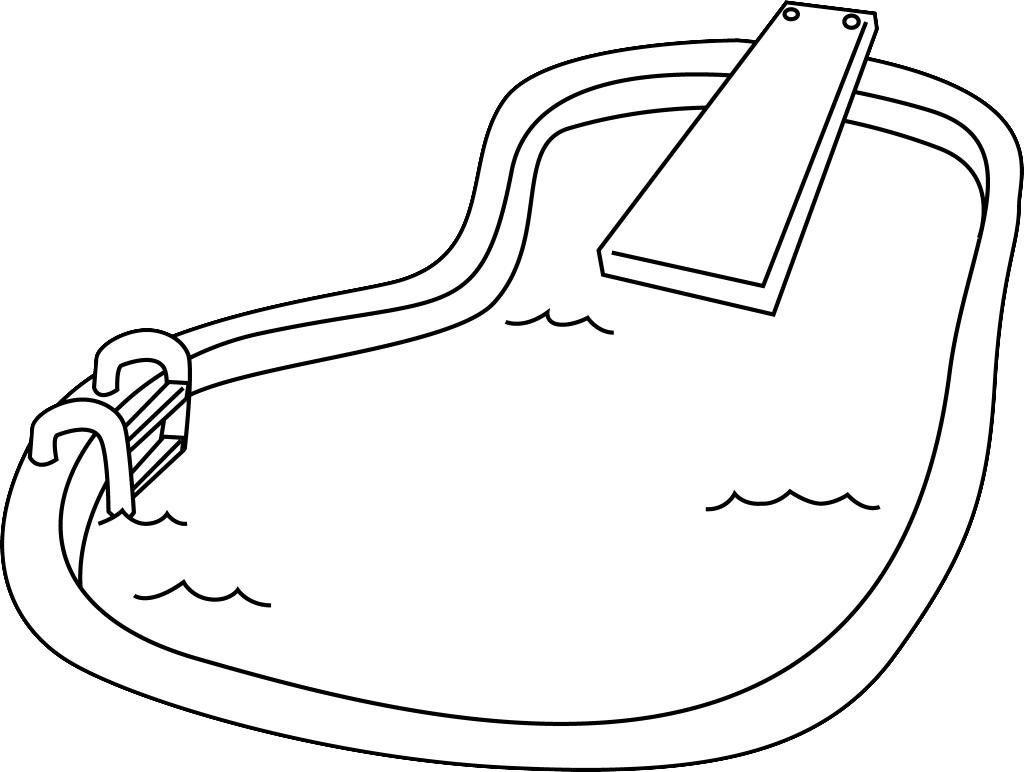
\includegraphics[width=0.4\textwidth]{figs/frontpage/smartpool.png}
\end{minipage}

\vspace{\fill}
\begin{minipage}[l]{\textwidth}
\begin{tabu} to \textwidth{lX[l]}
\textbf{Dato}           &\today\\
\textbf{Vejleder}		&Vejleder navn\\
\end{tabu}
\end{minipage}

\vspace{10pt}
\begin{minipage}[l]{\textwidth}
\tabulinesep=25pt
\begin{tabu} to \textwidth{X[l]X[l]X[l]}
 \makebox[\linewidth]{\hrulefill}\newline Joachim Dam Andersen     \newline 201370248/IKT  
&\makebox[\linewidth]{\hrulefill}\newline Lasse Priebe             \newline 201370248/IKT 
&\makebox[\linewidth]{\hrulefill}\newline Emil Nyborg              \newline 201370248/IKT\\
 \makebox[\linewidth]{\hrulefill}\newline Bjørn Nørgaard Sørensen  \newline 201370248/IKT  
&\makebox[\linewidth]{\hrulefill}\newline Alex Justesen Karlsen    \newline 201370248/IKT 
&\makebox[\linewidth]{\hrulefill}\newline Joachim Händel Noer Wind \newline 201370248/IKT
\end{tabu}
\end{minipage}\clearpage

%% Abstract
% Initial setup
\markboth{RESUMÉ/ABSTRACT}{RESUMÉ/ABSTRACT}
\abstractintoc
\abstractcol
\setlength{\abstitleskip}{-18pt}

% Abstract
\begin{abstract}
Rapporten omhandler et 3. semesterprojekt fra Ingeniørhøjskolen Aarhus Universitet udarbejdet med henblik på at producere et system, som kan fungere som dosering- og sorteringsanlæg til tabletter. Systemet er tiltænkt brug i ældreplejen, som en måde hvorpå fejlmedicinering kan undgås, og tabletsortering kan klares automatisk. Ydermere vil systemet kunne gøre personale og pårørende opmærksomme på, at brugeren ikke har afhentet sine tabletter, indenfor et givet tidsrum. Dette skal formidles ved hjælp af en Android applikation. Systemet og serveren samarbejder om at kontrollerer, hvad der dispenseres til den specifikke bruger og hvornår. Denne kommunikation er ikke fuldt ud implementeret endnu. Systemet var oprindeligt tiltænkt brug i private hjem, men undervejs i processen er idéen ændret idet at fokus flyttes fra private hjem til brug i plejesektoren. 
Produktet kan på nuværende tidspunkt dosere et bestemt antal tabletter af én enkelt type. Systemet har på nuværende tidspunkt allerede implementeret muligheden for at udvide med ekstra dispenserer, og er derfor velegnet til videreudvikling. 
Til systemet er der implementeret en fungerende brugergrænseflade, som er testet med en brugervenlighedsundersøgelse, der ved adspørgelse af 15 studerende har påpeget adskillige muligheder for forbedring.
Under systemudviklingen er den største arbejdsindsats lagt i undersøgelse af teknologier og mulige løsningsforslag.
\end{abstract}

\begin{abstracten}
The report covers a third semesterproject from the Aarhus University School of Engineering. The goal is to produce a system that can function as a dispensing and sorting machine for pills. The system is intended for use in eldercare, as a way of preventing medication errors and a way of sorting pills automaticly. Furthermore, the system will be able to notify staff and relatives if the elder has not picked up their pills, within a given timeperiod. The staff and relatives will be notified via an Android application. The system and a server operate together in order to control what is dispensed to whom and when. Though this communication is not fully implemented yet. The system was originally intended for use in private homes, but during the process, the idea evolved so that the focus was changed from home use to the healthcare sector.
The product can at this time dispense a certain number of pills which will have to be of a single type. The option of adding extra dispensers is already implemented, and is therefore suitable for further development.
The system also has a functioning interface implemented, which has been tested with a user-experience study in which 15 students participated. With the feedback made several things clear, and several of these are suitable for further work.
During the system development the largest effort was put into the study of technologies and potential solutions for the problem chosen.
\end{abstracten}\clearpage

%% Forord
\pagestyle{asereport}
\chapter{Forord}

% Forordet benyttes til at informere kort om visse ydre omstændigheder for projektet, såsom projekttype og hvor projektet er gennemført, historisk baggrund (andre arbejder, som har givet anledning til det aktuelle projekt) og hvor inspirationen og ideen er kommet fra, m.v.

Dette dokument er sammensat for at dokumentere arbejdet på 4. semesterprojektet for retningen IKT på ingeniørhøjskolen Århus.

Der vil i denne rapport være referencer til bilag og dokumentation, som det ikke ville være hensigtsmæssigt at medtage. Samtlige bilag m.m. vil være at finde på den vedlagt CD-rom. 

Source kode til projektet kan findes på CD'en. Link til vores github repo følger her: \newline \url{https://github.com/BjornNorgaard/DuckMaster3001}

\vspace{5mm}

\large{\textit{En stor tak til}}

\begin{displayquote}
    Lars Mortensen for god og brugbar vejledning.
\end{displayquote}

\begin{displayquote}
    Stjerne Apoteket for at lade gruppen komme på besøg og se deres sorteringsmaskine.
\end{displayquote}

\begin{displayquote}
    Sofie Fredslund for at lade os interviewe hende til projektet.
\end{displayquote}

\begin{displayquote}
   Underviserne på ASE, for hjælp og vejledning.
\end{displayquote}

\clearpage

%% ToC
\tableofcontents\clearpage

%% Indledning
\mainmatter
\chapter{Indledning}

Hello \cite{fysikbog} og sådan kan det jo gå.\clearpage

%% Projektformulering
%\documentclass[a4paper,11pt,oneside]{memoir}
%!TEX root = main.tex
% Encoding
%\usepackage[utf8]{inputenc} % pdfLatex
\usepackage[T1]{fontenc}
\usepackage[danish]{babel}
\renewcommand{\danishhyphenmins}{22}
\usepackage[utf8]{inputenc} % æ ø å

% Date
\usepackage[ddmmyyyy]{datetime}
\renewcommand{\dateseparator}{.}

% Fonts
\usepackage{fourier}
\usepackage[scaled=0.8]{beramono}

% Math
\usepackage{amsmath,amssymb}
\usepackage{bm}
\usepackage{amsthm}
\usepackage{mathtools}

% Graphics
\usepackage[usenames,dvipsnames,table]{xcolor}
\usepackage{graphicx}
\usepackage{float}
%\usepackage[section]{placeins}
\usepackage{tikz}
\usepackage[pages=some]{background}
\usepackage{wrapfig}

% Listings & Tables
\usepackage{listings}
%\usepackage{pythontex}
\usepackage{enumitem}
\usepackage{tabu}
\usepackage{longtable}
\usepackage{multirow}
\usepackage{makecell}


% References & Quotes
%\usepackage[danish]{varioref}				% Muliggoer bl.a. krydshenvisninger med sidetal (\vref)
%\usepackage{nat}							% Udvidelse med naturvidenskabelige citationsmodeller
\usepackage[danish=guillemets]{csquotes}
\usepackage[hidelinks]{hyperref}
\hypersetup{
    pdfstartview={FitH},
    pdftitle={Smart Pool 2.0},
    pdfsubject={Projektrapport},
    pdfauthor={I4PRJ4GRP3}
}
\usepackage[all]{hypcap}

% Etc
\usepackage[
	%backend=biber,
	backend=bibtex,
	style=ieee,
	natbib=true,
	backref=false,
	backrefstyle=all+,
	hyperref=true
]{biblatex}
\usepackage{pdflscape}
\usepackage[nomain,toc,xindy,acronym,nonumberlist,noredefwarn]{glossaries}
\usepackage[xindy]{imakeidx}
\usepackage{float}
\makeindex

% Dummy
\usepackage{lipsum}
%!TEX root = main.tex
% Page setup
\setulmarginsandblock{35mm}{25mm}{*}
\setlrmarginsandblock{20mm}{20mm}{*}
\setheadfoot{4\onelineskip}{2\onelineskip}
\setheaderspaces{*}{5mm}{*}
\checkandfixthelayout

% Pagestyle
\makepagestyle{asereport}
	\makeevenhead{asereport}{}{}{}
	\makeoddhead{asereport}{
\includegraphics{figs/frontpage/aseaulogo.pdf}}{}{\small\rightmark{} | \textbf{\thepage{}\vspace{7pt}}}
	\makeevenfoot{asereport}{}{}{}
	\makeoddfoot{asereport}{}{}{}

\makepsmarks{asereport}{
	\createmark{chapter}{both}{shownumber}{}{. \ }
	\createmark{section}{both}{shownumber}{}{. \ }
	\createmark{subsection}{both}{shownumber}{}{. \ }
	\createplainmark{toc}{both}{\contentsname}
	\createplainmark{lof}{both}{\listfigurename}
	\createplainmark{lot}{both}{\listtablename}
	\createplainmark{bib}{both}{\bibname}
	\createplainmark{index}{both}{\indexname}
	\createplainmark{glossary}{both}{\glossaryname}
}

\aliaspagestyle{part}{asereport}
\aliaspagestyle{chapter}{asereport}
\chapterstyle{tandh}

% Modification to certain spacing
\setlength{\parskip}{8pt}
\setlength{\parindent}{0pt}
\setlength{\abovecaptionskip}{7pt}
\setlength{\belowcaptionskip}{-10pt}
\OnehalfSpacing

% Tabu
%\taburowcolors[1]2{white .. light-gray}
\tabulinesep=4pt

% Itemize/enumerate
\setlist{
    before=\vspace{-3pt}, 
    after=\vspace{-3pt},
    itemsep=0pt,
    leftmargin=25pt,
    labelsep=10pt,
    topsep=0pt,
}

% Kommandoer til UC - fixer spacing
% Aktører
\newcommand{\fua}[1]{
	\begin{minipage}[t]{\linewidth}
		\setlist{
		    leftmargin=22pt,
		    itemsep=0pt,
		    topsep=0pt,
		    parsep=3pt
		}
	\begin{itemize}[before={\vspace{-6pt}}, after={\vspace{6pt}}]
	#1
	\end{itemize}
	\end{minipage}
}

% Hovedforløb
\newcommand{\fu}[1]{
\begin{minipage}[t]{\linewidth}
\setlist{
    leftmargin=22pt,
    itemsep=0pt,
    topsep=0pt,
    parsep=3pt
}
\raggedright
\begin{enumerate}[before={\vspace{-5pt}},after={\vspace{6pt}}]
#1
\end{enumerate}
\end{minipage}}

% Extensions
\newcommand{\fuex}[2]{
\begin{minipage}[t]{\linewidth}
\vspace{-6pt}
\raggedright
\textit{#1}
\begin{enumerate}[leftmargin=22pt,itemsep=0pt,parsep=3pt,before={\vspace{-8pt}}, after={\vspace{20pt}},topsep=8pt]
#2
\end{enumerate}
\end{minipage}
}

% Extensions - Sidste entry
\newcommand{\fuexl}[2]{
\begin{minipage}[t]{\linewidth}
\vspace{-6pt}
\raggedright
\textit{#1}
\begin{enumerate}[leftmargin=22pt,itemsep=0pt,parsep=3pt,before={\vspace{-8pt}}, after={\vspace{3pt}},topsep=8pt]
#2
\end{enumerate}
\end{minipage}}

% Versionshistorik
\newcommand{\verhistitem}[2]{
\begin{minipage}[t]{\linewidth}
\vspace{-6pt}
\raggedright
#1
\begin{itemize}[leftmargin=22pt,itemsep=0pt,parsep=0pt,before={\vspace{-10pt}},after={\vspace{3pt}},topsep=8pt]
#2
\end{itemize}
\end{minipage}}

\newcommand{\tverb}[1]{{\texttt{#1}}}

\newcommand{\cond}[1]{
\begin{itemize}[label=,noitemsep,topsep=0pt,after={\vspace*{-\baselineskip}}]
#1
\end{itemize}}

% Etc
\definecolor{light-gray}{gray}{0.8}
\definecolor{pantone}{RGB}{0,61,133}

\setfloatlocations{figure}{H}
\setfloatlocations{table}{H}

\numberwithin{equation}{chapter}
\numberwithin{figure}{chapter}
\setcounter{secnumdepth}{3}
\setcounter{tocdepth}{2}
\maxsecnumdepth{subsection}

\renewcommand*{\cftdotsep}{1}
\setpnumwidth{2em}
\setrmarg{2em}

\setverbatimfont{\ttfamily}

%\renewcommand\cftchaptername {\chaptername~}
%\renewcommand\cftappendixname {\appendixname~}
\addto\captionsdanish{
    \renewcommand\contentsname{Indholdsfortegnelse}
    \renewcommand\appendixname{Appendiks}
}
\renewcommand\appendixpagename{Appendiks}
\renewcommand\appendixtocname{Appendiks}
\newsubfloat{figure}

% Abstract
\newenvironment{abstracten}
{\renewcommand{\abstractname}{Abstract}\abstract}
{\endabstract}
\renewcommand{\abstractnamefont}{\normalfont\Large\bfseries}
%!TEX root = main.tex
% Listings
\AtBeginDocument{%
  \counterwithin*{lstlisting}{section}
  \counterwithin*{lstlisting}{subsection}
  \counterwithin*{lstlisting}{subsubsection}
  \renewcommand{\thelstlisting}{%
    \ifnum\value{subsection}=0
      \thesection.\arabic{lstlisting}%
    \else
      \ifnum\value{subsubsection}=0
        \thesubsection.\arabic{lstlisting}%
      \else
        \thesubsubsection.\arabic{lstlisting}%
      \fi
    \fi
  }
}

% Loading languages
\lstloadlanguages{C, C++}

% Listing setup
\lstdefinestyle{all}{
    basicstyle    = \ttfamily\SingleSpacing\scriptsize,
    numbers       = left, 
    numberstyle   = \ttfamily\tiny,
    breaklines    = true,
    commentstyle=\color{green},
    %backgroundcolor = \color{red},
    numbersep     = 20pt,
    xleftmargin   = \parindent,
    captionpos    = b,
    keywordstyle  = [1]\color{Blue}\bfseries,
    commentstyle  = \itshape\color{Green},
    tabsize       = 3
}

\lstset{
    style = all
} 
%!TEX root = main.tex
\makenoidxglossaries
\newglossaryentry{gui}{
    name={GUI}, 
    description={Graphical User Interface er en brugergrænseflade. Brugerens måde at tilgå systemet på}}

\newglossaryentry{psoc}{
    name={PSoC}, 
    description={PSoC (Programmable System-on-Chip) er et microcontroller system produceret af Cypress Semiconductor}}

\newglossaryentry{moscow}{
    name={MoSCoW}, 
    description={MoSCoW er en metode til at prioritere krav til ens system}}

\newglossaryentry{furps}{
    name={FURPS}, 
    description={FURPS er en metode til kategorisering af systemets ikke-funktionelle krav}}

\newglossaryentry{BDD}{
    name={BDD}, 
    description={BDD (Block Definition Diagram) er et diagram, som beskriver et system ved at opdele det op i mindre blokke}}

\newglossaryentry{IBD}{
    name={IBD}, 
    description={IBD (Internal Block Diagram) er et diagram, som viser forbindelserne mellem blokkene, som kan findes i et BDD}}

\newglossaryentry{pilleskuffe}{
    name={Pilleskuffe},
    description={Skuffen under dispenseren, hvor i den nederste pille ligger i. Skuffen tømmes ved at elektromagneten trækker skuffen til sig.}}

\newglossaryentry{pilledispenser}{
    name={Pilledispenser},
    description={Det rør som pillerne bliver opbevaret i.}}

\newglossaryentry{elektromagneten}{
    name={Elektromagneten},
    description={Elektromagneten er en spole der sendes strøm igennem. Når der er strøm på spolen dannes et magnetfelt. Der vil ofte være tale om det samme hvad enten der står spole eller elektromagnet.}}

%% Forside variabler
\newcommand{\Kursus}{I4PRJ4 F16}
\newcommand{\Projektnavn}{SmartPool 2.0}
\newcommand{\Gruppe}{Gruppe 3}
\newcommand{\Projektdokument}{Projektrapport}

%% Litteratur
\nocite{*}
%\bibliographystyle{harvard}
\bibliography{utils/litteratur}

\begin{document}
\frontmatter

%!TEX root = main.tex
\pagestyle{titlingpage}
\backgroundsetup{
	scale=1,
	angle=0,
	opacity=1,
	contents={
		\begin{tikzpicture}[remember picture,overlay]
		\path [fill=pantone] (-0.5\paperwidth,0.36\paperheight) rectangle (0.5\paperwidth,0.47\paperheight);  
		\path [fill=pantone] (-0.5\paperwidth,-0.47\paperheight) rectangle (0.5\paperwidth,-0.43\paperheight);  
		\end{tikzpicture}}}
\BgThispage
\vspace*{-25mm}
\begin{minipage}[l]{\textwidth}
	
\includegraphics[width=0.75\textwidth]{figs/frontpage/aseaulogohvid.pdf}
\end{minipage}

\vspace{35pt}
\begin{minipage}[l]{\textwidth}
\tabulinesep=10pt
\begin{tabu} to \textwidth{X[l]}
	{\small\MakeUppercase\Kursus}\\
	{\HUGE\bfseries\MakeUppercase\Projektnavn}\\
	{\Large\Gruppe}\\
	{\itshape\Projektdokument}
\end{tabu}
\end{minipage}

\vspace{5pt}
\begin{minipage}[l]{\textwidth}
    \centering
	\vspace*{0cm}\hspace*{8cm}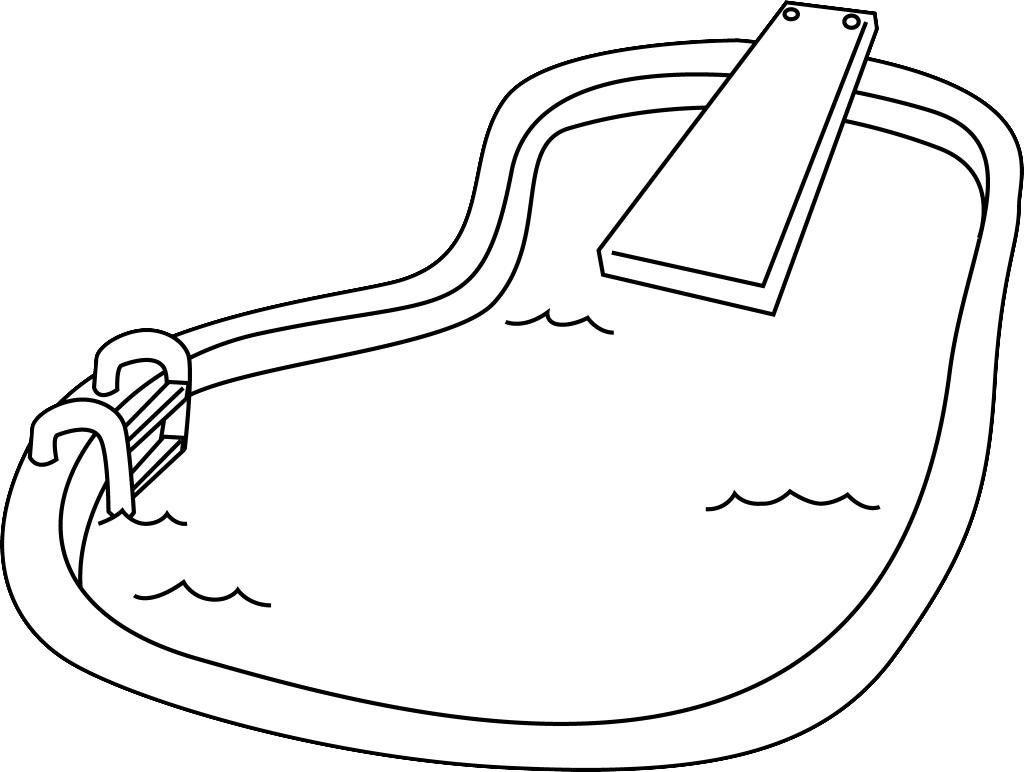
\includegraphics[width=0.4\textwidth]{figs/frontpage/smartpool.png}
\end{minipage}

\vspace{\fill}
\begin{minipage}[l]{\textwidth}
\begin{tabu} to \textwidth{lX[l]}
\textbf{Dato}           &\today\\
\textbf{Vejleder}		&Vejleder navn\\
\end{tabu}
\end{minipage}

\vspace{10pt}
\begin{minipage}[l]{\textwidth}
\tabulinesep=25pt
\begin{tabu} to \textwidth{X[l]X[l]X[l]}
 \makebox[\linewidth]{\hrulefill}\newline Joachim Dam Andersen     \newline 201370248/IKT  
&\makebox[\linewidth]{\hrulefill}\newline Lasse Priebe             \newline 201370248/IKT 
&\makebox[\linewidth]{\hrulefill}\newline Emil Nyborg              \newline 201370248/IKT\\
 \makebox[\linewidth]{\hrulefill}\newline Bjørn Nørgaard Sørensen  \newline 201370248/IKT  
&\makebox[\linewidth]{\hrulefill}\newline Alex Justesen Karlsen    \newline 201370248/IKT 
&\makebox[\linewidth]{\hrulefill}\newline Joachim Händel Noer Wind \newline 201370248/IKT
\end{tabu}
\end{minipage}\clearpage

%% Abstract
% Initial setup
\markboth{RESUMÉ/ABSTRACT}{RESUMÉ/ABSTRACT}
\abstractintoc
\abstractcol
\setlength{\abstitleskip}{-18pt}

% Abstract
\begin{abstract}
Rapporten omhandler et 3. semesterprojekt fra Ingeniørhøjskolen Aarhus Universitet udarbejdet med henblik på at producere et system, som kan fungere som dosering- og sorteringsanlæg til tabletter. Systemet er tiltænkt brug i ældreplejen, som en måde hvorpå fejlmedicinering kan undgås, og tabletsortering kan klares automatisk. Ydermere vil systemet kunne gøre personale og pårørende opmærksomme på, at brugeren ikke har afhentet sine tabletter, indenfor et givet tidsrum. Dette skal formidles ved hjælp af en Android applikation. Systemet og serveren samarbejder om at kontrollerer, hvad der dispenseres til den specifikke bruger og hvornår. Denne kommunikation er ikke fuldt ud implementeret endnu. Systemet var oprindeligt tiltænkt brug i private hjem, men undervejs i processen er idéen ændret idet at fokus flyttes fra private hjem til brug i plejesektoren. 
Produktet kan på nuværende tidspunkt dosere et bestemt antal tabletter af én enkelt type. Systemet har på nuværende tidspunkt allerede implementeret muligheden for at udvide med ekstra dispenserer, og er derfor velegnet til videreudvikling. 
Til systemet er der implementeret en fungerende brugergrænseflade, som er testet med en brugervenlighedsundersøgelse, der ved adspørgelse af 15 studerende har påpeget adskillige muligheder for forbedring.
Under systemudviklingen er den største arbejdsindsats lagt i undersøgelse af teknologier og mulige løsningsforslag.
\end{abstract}

\begin{abstracten}
The report covers a third semesterproject from the Aarhus University School of Engineering. The goal is to produce a system that can function as a dispensing and sorting machine for pills. The system is intended for use in eldercare, as a way of preventing medication errors and a way of sorting pills automaticly. Furthermore, the system will be able to notify staff and relatives if the elder has not picked up their pills, within a given timeperiod. The staff and relatives will be notified via an Android application. The system and a server operate together in order to control what is dispensed to whom and when. Though this communication is not fully implemented yet. The system was originally intended for use in private homes, but during the process, the idea evolved so that the focus was changed from home use to the healthcare sector.
The product can at this time dispense a certain number of pills which will have to be of a single type. The option of adding extra dispensers is already implemented, and is therefore suitable for further development.
The system also has a functioning interface implemented, which has been tested with a user-experience study in which 15 students participated. With the feedback made several things clear, and several of these are suitable for further work.
During the system development the largest effort was put into the study of technologies and potential solutions for the problem chosen.
\end{abstracten}\clearpage

%% Forord
\pagestyle{asereport}
\chapter{Forord}

% Forordet benyttes til at informere kort om visse ydre omstændigheder for projektet, såsom projekttype og hvor projektet er gennemført, historisk baggrund (andre arbejder, som har givet anledning til det aktuelle projekt) og hvor inspirationen og ideen er kommet fra, m.v.

Dette dokument er sammensat for at dokumentere arbejdet på 4. semesterprojektet for retningen IKT på ingeniørhøjskolen Århus.

Der vil i denne rapport være referencer til bilag og dokumentation, som det ikke ville være hensigtsmæssigt at medtage. Samtlige bilag m.m. vil være at finde på den vedlagt CD-rom. 

Source kode til projektet kan findes på CD'en. Link til vores github repo følger her: \newline \url{https://github.com/BjornNorgaard/DuckMaster3001}

\vspace{5mm}

\large{\textit{En stor tak til}}

\begin{displayquote}
    Lars Mortensen for god og brugbar vejledning.
\end{displayquote}

\begin{displayquote}
    Stjerne Apoteket for at lade gruppen komme på besøg og se deres sorteringsmaskine.
\end{displayquote}

\begin{displayquote}
    Sofie Fredslund for at lade os interviewe hende til projektet.
\end{displayquote}

\begin{displayquote}
   Underviserne på ASE, for hjælp og vejledning.
\end{displayquote}

\clearpage

%% ToC
\tableofcontents\clearpage

\mainmatter

%% Todo oversigt - SKAL UDKOMMENTERES FØR AFLEVERING
\listoftodos[Liste over gøremål]

%% Indledning
\chapter{Indledning}

Hello \cite{fysikbog} og sådan kan det jo gå.\clearpage

%% Projektformulering
\documentclass[a4paper,11pt,oneside]{memoir}
%!TEX root = main.tex
% Encoding
%\usepackage[utf8]{inputenc} % pdfLatex
\usepackage[T1]{fontenc}
\usepackage[danish]{babel}
\renewcommand{\danishhyphenmins}{22}
\usepackage[utf8]{inputenc} % æ ø å

% Date
\usepackage[ddmmyyyy]{datetime}
\renewcommand{\dateseparator}{.}

% Fonts
\usepackage{fourier}
\usepackage[scaled=0.8]{beramono}

% Math
\usepackage{amsmath,amssymb}
\usepackage{bm}
\usepackage{amsthm}
\usepackage{mathtools}

% Graphics
\usepackage[usenames,dvipsnames,table]{xcolor}
\usepackage{graphicx}
\usepackage{float}
%\usepackage[section]{placeins}
\usepackage{tikz}
\usepackage[pages=some]{background}
\usepackage{wrapfig}

% Listings & Tables
\usepackage{listings}
%\usepackage{pythontex}
\usepackage{enumitem}
\usepackage{tabu}
\usepackage{longtable}
\usepackage{multirow}
\usepackage{makecell}


% References & Quotes
%\usepackage[danish]{varioref}				% Muliggoer bl.a. krydshenvisninger med sidetal (\vref)
%\usepackage{nat}							% Udvidelse med naturvidenskabelige citationsmodeller
\usepackage[danish=guillemets]{csquotes}
\usepackage[hidelinks]{hyperref}
\hypersetup{
    pdfstartview={FitH},
    pdftitle={Smart Pool 2.0},
    pdfsubject={Projektrapport},
    pdfauthor={I4PRJ4GRP3}
}
\usepackage[all]{hypcap}

% Etc
\usepackage[
	%backend=biber,
	backend=bibtex,
	style=ieee,
	natbib=true,
	backref=false,
	backrefstyle=all+,
	hyperref=true
]{biblatex}
\usepackage{pdflscape}
\usepackage[nomain,toc,xindy,acronym,nonumberlist,noredefwarn]{glossaries}
\usepackage[xindy]{imakeidx}
\usepackage{float}
\makeindex

% Dummy
\usepackage{lipsum}
%!TEX root = main.tex
% Page setup
\setulmarginsandblock{35mm}{25mm}{*}
\setlrmarginsandblock{20mm}{20mm}{*}
\setheadfoot{4\onelineskip}{2\onelineskip}
\setheaderspaces{*}{5mm}{*}
\checkandfixthelayout

% Pagestyle
\makepagestyle{asereport}
	\makeevenhead{asereport}{}{}{}
	\makeoddhead{asereport}{
\includegraphics{figs/frontpage/aseaulogo.pdf}}{}{\small\rightmark{} | \textbf{\thepage{}\vspace{7pt}}}
	\makeevenfoot{asereport}{}{}{}
	\makeoddfoot{asereport}{}{}{}

\makepsmarks{asereport}{
	\createmark{chapter}{both}{shownumber}{}{. \ }
	\createmark{section}{both}{shownumber}{}{. \ }
	\createmark{subsection}{both}{shownumber}{}{. \ }
	\createplainmark{toc}{both}{\contentsname}
	\createplainmark{lof}{both}{\listfigurename}
	\createplainmark{lot}{both}{\listtablename}
	\createplainmark{bib}{both}{\bibname}
	\createplainmark{index}{both}{\indexname}
	\createplainmark{glossary}{both}{\glossaryname}
}

\aliaspagestyle{part}{asereport}
\aliaspagestyle{chapter}{asereport}
\chapterstyle{tandh}

% Modification to certain spacing
\setlength{\parskip}{8pt}
\setlength{\parindent}{0pt}
\setlength{\abovecaptionskip}{7pt}
\setlength{\belowcaptionskip}{-10pt}
\OnehalfSpacing

% Tabu
%\taburowcolors[1]2{white .. light-gray}
\tabulinesep=4pt

% Itemize/enumerate
\setlist{
    before=\vspace{-3pt}, 
    after=\vspace{-3pt},
    itemsep=0pt,
    leftmargin=25pt,
    labelsep=10pt,
    topsep=0pt,
}

% Kommandoer til UC - fixer spacing
% Aktører
\newcommand{\fua}[1]{
	\begin{minipage}[t]{\linewidth}
		\setlist{
		    leftmargin=22pt,
		    itemsep=0pt,
		    topsep=0pt,
		    parsep=3pt
		}
	\begin{itemize}[before={\vspace{-6pt}}, after={\vspace{6pt}}]
	#1
	\end{itemize}
	\end{minipage}
}

% Hovedforløb
\newcommand{\fu}[1]{
\begin{minipage}[t]{\linewidth}
\setlist{
    leftmargin=22pt,
    itemsep=0pt,
    topsep=0pt,
    parsep=3pt
}
\raggedright
\begin{enumerate}[before={\vspace{-5pt}},after={\vspace{6pt}}]
#1
\end{enumerate}
\end{minipage}}

% Extensions
\newcommand{\fuex}[2]{
\begin{minipage}[t]{\linewidth}
\vspace{-6pt}
\raggedright
\textit{#1}
\begin{enumerate}[leftmargin=22pt,itemsep=0pt,parsep=3pt,before={\vspace{-8pt}}, after={\vspace{20pt}},topsep=8pt]
#2
\end{enumerate}
\end{minipage}
}

% Extensions - Sidste entry
\newcommand{\fuexl}[2]{
\begin{minipage}[t]{\linewidth}
\vspace{-6pt}
\raggedright
\textit{#1}
\begin{enumerate}[leftmargin=22pt,itemsep=0pt,parsep=3pt,before={\vspace{-8pt}}, after={\vspace{3pt}},topsep=8pt]
#2
\end{enumerate}
\end{minipage}}

% Versionshistorik
\newcommand{\verhistitem}[2]{
\begin{minipage}[t]{\linewidth}
\vspace{-6pt}
\raggedright
#1
\begin{itemize}[leftmargin=22pt,itemsep=0pt,parsep=0pt,before={\vspace{-10pt}},after={\vspace{3pt}},topsep=8pt]
#2
\end{itemize}
\end{minipage}}

\newcommand{\tverb}[1]{{\texttt{#1}}}

\newcommand{\cond}[1]{
\begin{itemize}[label=,noitemsep,topsep=0pt,after={\vspace*{-\baselineskip}}]
#1
\end{itemize}}

% Etc
\definecolor{light-gray}{gray}{0.8}
\definecolor{pantone}{RGB}{0,61,133}

\setfloatlocations{figure}{H}
\setfloatlocations{table}{H}

\numberwithin{equation}{chapter}
\numberwithin{figure}{chapter}
\setcounter{secnumdepth}{3}
\setcounter{tocdepth}{2}
\maxsecnumdepth{subsection}

\renewcommand*{\cftdotsep}{1}
\setpnumwidth{2em}
\setrmarg{2em}

\setverbatimfont{\ttfamily}

%\renewcommand\cftchaptername {\chaptername~}
%\renewcommand\cftappendixname {\appendixname~}
\addto\captionsdanish{
    \renewcommand\contentsname{Indholdsfortegnelse}
    \renewcommand\appendixname{Appendiks}
}
\renewcommand\appendixpagename{Appendiks}
\renewcommand\appendixtocname{Appendiks}
\newsubfloat{figure}

% Abstract
\newenvironment{abstracten}
{\renewcommand{\abstractname}{Abstract}\abstract}
{\endabstract}
\renewcommand{\abstractnamefont}{\normalfont\Large\bfseries}
%!TEX root = main.tex
% Listings
\AtBeginDocument{%
  \counterwithin*{lstlisting}{section}
  \counterwithin*{lstlisting}{subsection}
  \counterwithin*{lstlisting}{subsubsection}
  \renewcommand{\thelstlisting}{%
    \ifnum\value{subsection}=0
      \thesection.\arabic{lstlisting}%
    \else
      \ifnum\value{subsubsection}=0
        \thesubsection.\arabic{lstlisting}%
      \else
        \thesubsubsection.\arabic{lstlisting}%
      \fi
    \fi
  }
}

% Loading languages
\lstloadlanguages{C, C++}

% Listing setup
\lstdefinestyle{all}{
    basicstyle    = \ttfamily\SingleSpacing\scriptsize,
    numbers       = left, 
    numberstyle   = \ttfamily\tiny,
    breaklines    = true,
    commentstyle=\color{green},
    %backgroundcolor = \color{red},
    numbersep     = 20pt,
    xleftmargin   = \parindent,
    captionpos    = b,
    keywordstyle  = [1]\color{Blue}\bfseries,
    commentstyle  = \itshape\color{Green},
    tabsize       = 3
}

\lstset{
    style = all
} 
%!TEX root = main.tex
\makenoidxglossaries
\newglossaryentry{gui}{
    name={GUI}, 
    description={Graphical User Interface er en brugergrænseflade. Brugerens måde at tilgå systemet på}}

\newglossaryentry{psoc}{
    name={PSoC}, 
    description={PSoC (Programmable System-on-Chip) er et microcontroller system produceret af Cypress Semiconductor}}

\newglossaryentry{moscow}{
    name={MoSCoW}, 
    description={MoSCoW er en metode til at prioritere krav til ens system}}

\newglossaryentry{furps}{
    name={FURPS}, 
    description={FURPS er en metode til kategorisering af systemets ikke-funktionelle krav}}

\newglossaryentry{BDD}{
    name={BDD}, 
    description={BDD (Block Definition Diagram) er et diagram, som beskriver et system ved at opdele det op i mindre blokke}}

\newglossaryentry{IBD}{
    name={IBD}, 
    description={IBD (Internal Block Diagram) er et diagram, som viser forbindelserne mellem blokkene, som kan findes i et BDD}}

\newglossaryentry{pilleskuffe}{
    name={Pilleskuffe},
    description={Skuffen under dispenseren, hvor i den nederste pille ligger i. Skuffen tømmes ved at elektromagneten trækker skuffen til sig.}}

\newglossaryentry{pilledispenser}{
    name={Pilledispenser},
    description={Det rør som pillerne bliver opbevaret i.}}

\newglossaryentry{elektromagneten}{
    name={Elektromagneten},
    description={Elektromagneten er en spole der sendes strøm igennem. Når der er strøm på spolen dannes et magnetfelt. Der vil ofte være tale om det samme hvad enten der står spole eller elektromagnet.}}

%% Forside variabler
\newcommand{\Kursus}{I4PRJ4 F16}
\newcommand{\Projektnavn}{SmartPool 2.0}
\newcommand{\Gruppe}{Gruppe 3}
\newcommand{\Projektdokument}{Projektrapport}

%% Litteratur
\nocite{*}
%\bibliographystyle{harvard}
\bibliography{utils/litteratur}

\begin{document}
\frontmatter

%!TEX root = main.tex
\pagestyle{titlingpage}
\backgroundsetup{
	scale=1,
	angle=0,
	opacity=1,
	contents={
		\begin{tikzpicture}[remember picture,overlay]
		\path [fill=pantone] (-0.5\paperwidth,0.36\paperheight) rectangle (0.5\paperwidth,0.47\paperheight);  
		\path [fill=pantone] (-0.5\paperwidth,-0.47\paperheight) rectangle (0.5\paperwidth,-0.43\paperheight);  
		\end{tikzpicture}}}
\BgThispage
\vspace*{-25mm}
\begin{minipage}[l]{\textwidth}
	
\includegraphics[width=0.75\textwidth]{figs/frontpage/aseaulogohvid.pdf}
\end{minipage}

\vspace{35pt}
\begin{minipage}[l]{\textwidth}
\tabulinesep=10pt
\begin{tabu} to \textwidth{X[l]}
	{\small\MakeUppercase\Kursus}\\
	{\HUGE\bfseries\MakeUppercase\Projektnavn}\\
	{\Large\Gruppe}\\
	{\itshape\Projektdokument}
\end{tabu}
\end{minipage}

\vspace{5pt}
\begin{minipage}[l]{\textwidth}
    \centering
	\vspace*{0cm}\hspace*{8cm}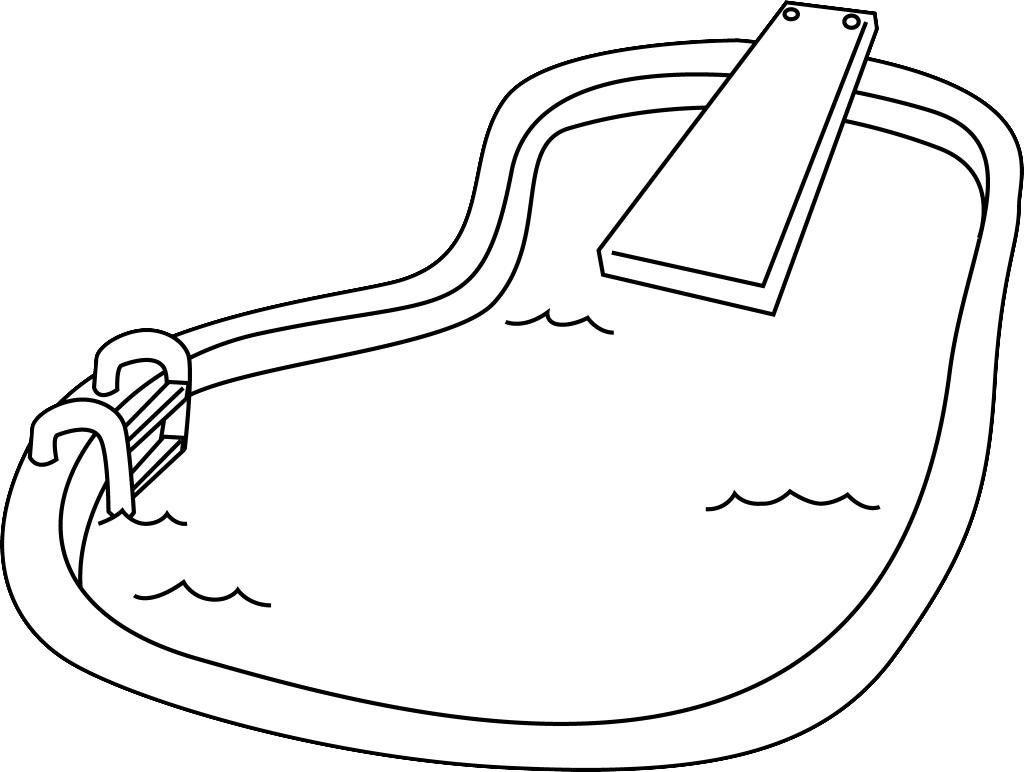
\includegraphics[width=0.4\textwidth]{figs/frontpage/smartpool.png}
\end{minipage}

\vspace{\fill}
\begin{minipage}[l]{\textwidth}
\begin{tabu} to \textwidth{lX[l]}
\textbf{Dato}           &\today\\
\textbf{Vejleder}		&Vejleder navn\\
\end{tabu}
\end{minipage}

\vspace{10pt}
\begin{minipage}[l]{\textwidth}
\tabulinesep=25pt
\begin{tabu} to \textwidth{X[l]X[l]X[l]}
 \makebox[\linewidth]{\hrulefill}\newline Joachim Dam Andersen     \newline 201370248/IKT  
&\makebox[\linewidth]{\hrulefill}\newline Lasse Priebe             \newline 201370248/IKT 
&\makebox[\linewidth]{\hrulefill}\newline Emil Nyborg              \newline 201370248/IKT\\
 \makebox[\linewidth]{\hrulefill}\newline Bjørn Nørgaard Sørensen  \newline 201370248/IKT  
&\makebox[\linewidth]{\hrulefill}\newline Alex Justesen Karlsen    \newline 201370248/IKT 
&\makebox[\linewidth]{\hrulefill}\newline Joachim Händel Noer Wind \newline 201370248/IKT
\end{tabu}
\end{minipage}\clearpage

%% Abstract
% Initial setup
\markboth{RESUMÉ/ABSTRACT}{RESUMÉ/ABSTRACT}
\abstractintoc
\abstractcol
\setlength{\abstitleskip}{-18pt}

% Abstract
\begin{abstract}
Rapporten omhandler et 3. semesterprojekt fra Ingeniørhøjskolen Aarhus Universitet udarbejdet med henblik på at producere et system, som kan fungere som dosering- og sorteringsanlæg til tabletter. Systemet er tiltænkt brug i ældreplejen, som en måde hvorpå fejlmedicinering kan undgås, og tabletsortering kan klares automatisk. Ydermere vil systemet kunne gøre personale og pårørende opmærksomme på, at brugeren ikke har afhentet sine tabletter, indenfor et givet tidsrum. Dette skal formidles ved hjælp af en Android applikation. Systemet og serveren samarbejder om at kontrollerer, hvad der dispenseres til den specifikke bruger og hvornår. Denne kommunikation er ikke fuldt ud implementeret endnu. Systemet var oprindeligt tiltænkt brug i private hjem, men undervejs i processen er idéen ændret idet at fokus flyttes fra private hjem til brug i plejesektoren. 
Produktet kan på nuværende tidspunkt dosere et bestemt antal tabletter af én enkelt type. Systemet har på nuværende tidspunkt allerede implementeret muligheden for at udvide med ekstra dispenserer, og er derfor velegnet til videreudvikling. 
Til systemet er der implementeret en fungerende brugergrænseflade, som er testet med en brugervenlighedsundersøgelse, der ved adspørgelse af 15 studerende har påpeget adskillige muligheder for forbedring.
Under systemudviklingen er den største arbejdsindsats lagt i undersøgelse af teknologier og mulige løsningsforslag.
\end{abstract}

\begin{abstracten}
The report covers a third semesterproject from the Aarhus University School of Engineering. The goal is to produce a system that can function as a dispensing and sorting machine for pills. The system is intended for use in eldercare, as a way of preventing medication errors and a way of sorting pills automaticly. Furthermore, the system will be able to notify staff and relatives if the elder has not picked up their pills, within a given timeperiod. The staff and relatives will be notified via an Android application. The system and a server operate together in order to control what is dispensed to whom and when. Though this communication is not fully implemented yet. The system was originally intended for use in private homes, but during the process, the idea evolved so that the focus was changed from home use to the healthcare sector.
The product can at this time dispense a certain number of pills which will have to be of a single type. The option of adding extra dispensers is already implemented, and is therefore suitable for further development.
The system also has a functioning interface implemented, which has been tested with a user-experience study in which 15 students participated. With the feedback made several things clear, and several of these are suitable for further work.
During the system development the largest effort was put into the study of technologies and potential solutions for the problem chosen.
\end{abstracten}\clearpage

%% Forord
\pagestyle{asereport}
\chapter{Forord}

% Forordet benyttes til at informere kort om visse ydre omstændigheder for projektet, såsom projekttype og hvor projektet er gennemført, historisk baggrund (andre arbejder, som har givet anledning til det aktuelle projekt) og hvor inspirationen og ideen er kommet fra, m.v.

Dette dokument er sammensat for at dokumentere arbejdet på 4. semesterprojektet for retningen IKT på ingeniørhøjskolen Århus.

Der vil i denne rapport være referencer til bilag og dokumentation, som det ikke ville være hensigtsmæssigt at medtage. Samtlige bilag m.m. vil være at finde på den vedlagt CD-rom. 

Source kode til projektet kan findes på CD'en. Link til vores github repo følger her: \newline \url{https://github.com/BjornNorgaard/DuckMaster3001}

\vspace{5mm}

\large{\textit{En stor tak til}}

\begin{displayquote}
    Lars Mortensen for god og brugbar vejledning.
\end{displayquote}

\begin{displayquote}
    Stjerne Apoteket for at lade gruppen komme på besøg og se deres sorteringsmaskine.
\end{displayquote}

\begin{displayquote}
    Sofie Fredslund for at lade os interviewe hende til projektet.
\end{displayquote}

\begin{displayquote}
   Underviserne på ASE, for hjælp og vejledning.
\end{displayquote}

\clearpage

%% ToC
\tableofcontents\clearpage

\mainmatter

%% Todo oversigt - SKAL UDKOMMENTERES FØR AFLEVERING
\listoftodos[Liste over gøremål]

%% Indledning
\chapter{Indledning}

Hello \cite{fysikbog} og sådan kan det jo gå.\clearpage

%% Projektformulering
\documentclass[a4paper,11pt,oneside]{memoir}
\input{utils/packages}
\input{utils/layout}
\input{utils/listings}
\input{utils/ordliste}

%% Forside variabler
\newcommand{\Kursus}{I4PRJ4 F16}
\newcommand{\Projektnavn}{SmartPool 2.0}
\newcommand{\Gruppe}{Gruppe 3}
\newcommand{\Projektdokument}{Projektrapport}

%% Litteratur
\nocite{*}
%\bibliographystyle{harvard}
\bibliography{utils/litteratur}

\begin{document}
\frontmatter

\input{utils/frontpage}\clearpage

%% Abstract
\input{docs/frontmatter/abstract}\clearpage

%% Forord
\pagestyle{asereport}
\input{docs/frontmatter/forord}\clearpage

%% ToC
\tableofcontents\clearpage

\mainmatter

%% Todo oversigt - SKAL UDKOMMENTERES FØR AFLEVERING
\listoftodos[Liste over gøremål]

%% Indledning
\input{docs/frontmatter/indledning}\clearpage

%% Projektformulering
\input{docs/projektformulering/main}\clearpage

%% Kravspecifikation
\input{docs/kravspecifikation/main}\clearpage

%% Systemarkitektur
\input{docs/systemarkitektur/main}\clearpage

%% Processbeskrivelse
\input{docs/processbeskrivelse/main}\clearpage

%% Design
\input{docs/design/main}\clearpage

%% Implementering
\input{docs/implementering/main}\clearpage

%% Integration
\input{docs/integration/main}\clearpage

%% Accepttest
\input{docs/accepttest/main}\clearpage

%% Appendix
\input{docs/appendix/main}\clearpage

\backmatter
%% Glossary
\setglossarystyle{list}
\printnoidxglossary[title=Ordliste]

% Bibliography
\clearpage
\printbibliography[title={Litteratur}]
\end{document}\clearpage

%% Kravspecifikation
\documentclass[a4paper,11pt,oneside]{memoir}
\input{utils/packages}
\input{utils/layout}
\input{utils/listings}
\input{utils/ordliste}

%% Forside variabler
\newcommand{\Kursus}{I4PRJ4 F16}
\newcommand{\Projektnavn}{SmartPool 2.0}
\newcommand{\Gruppe}{Gruppe 3}
\newcommand{\Projektdokument}{Projektrapport}

%% Litteratur
\nocite{*}
%\bibliographystyle{harvard}
\bibliography{utils/litteratur}

\begin{document}
\frontmatter

\input{utils/frontpage}\clearpage

%% Abstract
\input{docs/frontmatter/abstract}\clearpage

%% Forord
\pagestyle{asereport}
\input{docs/frontmatter/forord}\clearpage

%% ToC
\tableofcontents\clearpage

\mainmatter

%% Todo oversigt - SKAL UDKOMMENTERES FØR AFLEVERING
\listoftodos[Liste over gøremål]

%% Indledning
\input{docs/frontmatter/indledning}\clearpage

%% Projektformulering
\input{docs/projektformulering/main}\clearpage

%% Kravspecifikation
\input{docs/kravspecifikation/main}\clearpage

%% Systemarkitektur
\input{docs/systemarkitektur/main}\clearpage

%% Processbeskrivelse
\input{docs/processbeskrivelse/main}\clearpage

%% Design
\input{docs/design/main}\clearpage

%% Implementering
\input{docs/implementering/main}\clearpage

%% Integration
\input{docs/integration/main}\clearpage

%% Accepttest
\input{docs/accepttest/main}\clearpage

%% Appendix
\input{docs/appendix/main}\clearpage

\backmatter
%% Glossary
\setglossarystyle{list}
\printnoidxglossary[title=Ordliste]

% Bibliography
\clearpage
\printbibliography[title={Litteratur}]
\end{document}\clearpage

%% Systemarkitektur
\documentclass[a4paper,11pt,oneside]{memoir}
\input{utils/packages}
\input{utils/layout}
\input{utils/listings}
\input{utils/ordliste}

%% Forside variabler
\newcommand{\Kursus}{I4PRJ4 F16}
\newcommand{\Projektnavn}{SmartPool 2.0}
\newcommand{\Gruppe}{Gruppe 3}
\newcommand{\Projektdokument}{Projektrapport}

%% Litteratur
\nocite{*}
%\bibliographystyle{harvard}
\bibliography{utils/litteratur}

\begin{document}
\frontmatter

\input{utils/frontpage}\clearpage

%% Abstract
\input{docs/frontmatter/abstract}\clearpage

%% Forord
\pagestyle{asereport}
\input{docs/frontmatter/forord}\clearpage

%% ToC
\tableofcontents\clearpage

\mainmatter

%% Todo oversigt - SKAL UDKOMMENTERES FØR AFLEVERING
\listoftodos[Liste over gøremål]

%% Indledning
\input{docs/frontmatter/indledning}\clearpage

%% Projektformulering
\input{docs/projektformulering/main}\clearpage

%% Kravspecifikation
\input{docs/kravspecifikation/main}\clearpage

%% Systemarkitektur
\input{docs/systemarkitektur/main}\clearpage

%% Processbeskrivelse
\input{docs/processbeskrivelse/main}\clearpage

%% Design
\input{docs/design/main}\clearpage

%% Implementering
\input{docs/implementering/main}\clearpage

%% Integration
\input{docs/integration/main}\clearpage

%% Accepttest
\input{docs/accepttest/main}\clearpage

%% Appendix
\input{docs/appendix/main}\clearpage

\backmatter
%% Glossary
\setglossarystyle{list}
\printnoidxglossary[title=Ordliste]

% Bibliography
\clearpage
\printbibliography[title={Litteratur}]
\end{document}\clearpage

%% Processbeskrivelse
\documentclass[a4paper,11pt,oneside]{memoir}
\input{utils/packages}
\input{utils/layout}
\input{utils/listings}
\input{utils/ordliste}

%% Forside variabler
\newcommand{\Kursus}{I4PRJ4 F16}
\newcommand{\Projektnavn}{SmartPool 2.0}
\newcommand{\Gruppe}{Gruppe 3}
\newcommand{\Projektdokument}{Projektrapport}

%% Litteratur
\nocite{*}
%\bibliographystyle{harvard}
\bibliography{utils/litteratur}

\begin{document}
\frontmatter

\input{utils/frontpage}\clearpage

%% Abstract
\input{docs/frontmatter/abstract}\clearpage

%% Forord
\pagestyle{asereport}
\input{docs/frontmatter/forord}\clearpage

%% ToC
\tableofcontents\clearpage

\mainmatter

%% Todo oversigt - SKAL UDKOMMENTERES FØR AFLEVERING
\listoftodos[Liste over gøremål]

%% Indledning
\input{docs/frontmatter/indledning}\clearpage

%% Projektformulering
\input{docs/projektformulering/main}\clearpage

%% Kravspecifikation
\input{docs/kravspecifikation/main}\clearpage

%% Systemarkitektur
\input{docs/systemarkitektur/main}\clearpage

%% Processbeskrivelse
\input{docs/processbeskrivelse/main}\clearpage

%% Design
\input{docs/design/main}\clearpage

%% Implementering
\input{docs/implementering/main}\clearpage

%% Integration
\input{docs/integration/main}\clearpage

%% Accepttest
\input{docs/accepttest/main}\clearpage

%% Appendix
\input{docs/appendix/main}\clearpage

\backmatter
%% Glossary
\setglossarystyle{list}
\printnoidxglossary[title=Ordliste]

% Bibliography
\clearpage
\printbibliography[title={Litteratur}]
\end{document}\clearpage

%% Design
\documentclass[a4paper,11pt,oneside]{memoir}
\input{utils/packages}
\input{utils/layout}
\input{utils/listings}
\input{utils/ordliste}

%% Forside variabler
\newcommand{\Kursus}{I4PRJ4 F16}
\newcommand{\Projektnavn}{SmartPool 2.0}
\newcommand{\Gruppe}{Gruppe 3}
\newcommand{\Projektdokument}{Projektrapport}

%% Litteratur
\nocite{*}
%\bibliographystyle{harvard}
\bibliography{utils/litteratur}

\begin{document}
\frontmatter

\input{utils/frontpage}\clearpage

%% Abstract
\input{docs/frontmatter/abstract}\clearpage

%% Forord
\pagestyle{asereport}
\input{docs/frontmatter/forord}\clearpage

%% ToC
\tableofcontents\clearpage

\mainmatter

%% Todo oversigt - SKAL UDKOMMENTERES FØR AFLEVERING
\listoftodos[Liste over gøremål]

%% Indledning
\input{docs/frontmatter/indledning}\clearpage

%% Projektformulering
\input{docs/projektformulering/main}\clearpage

%% Kravspecifikation
\input{docs/kravspecifikation/main}\clearpage

%% Systemarkitektur
\input{docs/systemarkitektur/main}\clearpage

%% Processbeskrivelse
\input{docs/processbeskrivelse/main}\clearpage

%% Design
\input{docs/design/main}\clearpage

%% Implementering
\input{docs/implementering/main}\clearpage

%% Integration
\input{docs/integration/main}\clearpage

%% Accepttest
\input{docs/accepttest/main}\clearpage

%% Appendix
\input{docs/appendix/main}\clearpage

\backmatter
%% Glossary
\setglossarystyle{list}
\printnoidxglossary[title=Ordliste]

% Bibliography
\clearpage
\printbibliography[title={Litteratur}]
\end{document}\clearpage

%% Implementering
\documentclass[a4paper,11pt,oneside]{memoir}
\input{utils/packages}
\input{utils/layout}
\input{utils/listings}
\input{utils/ordliste}

%% Forside variabler
\newcommand{\Kursus}{I4PRJ4 F16}
\newcommand{\Projektnavn}{SmartPool 2.0}
\newcommand{\Gruppe}{Gruppe 3}
\newcommand{\Projektdokument}{Projektrapport}

%% Litteratur
\nocite{*}
%\bibliographystyle{harvard}
\bibliography{utils/litteratur}

\begin{document}
\frontmatter

\input{utils/frontpage}\clearpage

%% Abstract
\input{docs/frontmatter/abstract}\clearpage

%% Forord
\pagestyle{asereport}
\input{docs/frontmatter/forord}\clearpage

%% ToC
\tableofcontents\clearpage

\mainmatter

%% Todo oversigt - SKAL UDKOMMENTERES FØR AFLEVERING
\listoftodos[Liste over gøremål]

%% Indledning
\input{docs/frontmatter/indledning}\clearpage

%% Projektformulering
\input{docs/projektformulering/main}\clearpage

%% Kravspecifikation
\input{docs/kravspecifikation/main}\clearpage

%% Systemarkitektur
\input{docs/systemarkitektur/main}\clearpage

%% Processbeskrivelse
\input{docs/processbeskrivelse/main}\clearpage

%% Design
\input{docs/design/main}\clearpage

%% Implementering
\input{docs/implementering/main}\clearpage

%% Integration
\input{docs/integration/main}\clearpage

%% Accepttest
\input{docs/accepttest/main}\clearpage

%% Appendix
\input{docs/appendix/main}\clearpage

\backmatter
%% Glossary
\setglossarystyle{list}
\printnoidxglossary[title=Ordliste]

% Bibliography
\clearpage
\printbibliography[title={Litteratur}]
\end{document}\clearpage

%% Integration
\documentclass[a4paper,11pt,oneside]{memoir}
\input{utils/packages}
\input{utils/layout}
\input{utils/listings}
\input{utils/ordliste}

%% Forside variabler
\newcommand{\Kursus}{I4PRJ4 F16}
\newcommand{\Projektnavn}{SmartPool 2.0}
\newcommand{\Gruppe}{Gruppe 3}
\newcommand{\Projektdokument}{Projektrapport}

%% Litteratur
\nocite{*}
%\bibliographystyle{harvard}
\bibliography{utils/litteratur}

\begin{document}
\frontmatter

\input{utils/frontpage}\clearpage

%% Abstract
\input{docs/frontmatter/abstract}\clearpage

%% Forord
\pagestyle{asereport}
\input{docs/frontmatter/forord}\clearpage

%% ToC
\tableofcontents\clearpage

\mainmatter

%% Todo oversigt - SKAL UDKOMMENTERES FØR AFLEVERING
\listoftodos[Liste over gøremål]

%% Indledning
\input{docs/frontmatter/indledning}\clearpage

%% Projektformulering
\input{docs/projektformulering/main}\clearpage

%% Kravspecifikation
\input{docs/kravspecifikation/main}\clearpage

%% Systemarkitektur
\input{docs/systemarkitektur/main}\clearpage

%% Processbeskrivelse
\input{docs/processbeskrivelse/main}\clearpage

%% Design
\input{docs/design/main}\clearpage

%% Implementering
\input{docs/implementering/main}\clearpage

%% Integration
\input{docs/integration/main}\clearpage

%% Accepttest
\input{docs/accepttest/main}\clearpage

%% Appendix
\input{docs/appendix/main}\clearpage

\backmatter
%% Glossary
\setglossarystyle{list}
\printnoidxglossary[title=Ordliste]

% Bibliography
\clearpage
\printbibliography[title={Litteratur}]
\end{document}\clearpage

%% Accepttest
\documentclass[a4paper,11pt,oneside]{memoir}
\input{utils/packages}
\input{utils/layout}
\input{utils/listings}
\input{utils/ordliste}

%% Forside variabler
\newcommand{\Kursus}{I4PRJ4 F16}
\newcommand{\Projektnavn}{SmartPool 2.0}
\newcommand{\Gruppe}{Gruppe 3}
\newcommand{\Projektdokument}{Projektrapport}

%% Litteratur
\nocite{*}
%\bibliographystyle{harvard}
\bibliography{utils/litteratur}

\begin{document}
\frontmatter

\input{utils/frontpage}\clearpage

%% Abstract
\input{docs/frontmatter/abstract}\clearpage

%% Forord
\pagestyle{asereport}
\input{docs/frontmatter/forord}\clearpage

%% ToC
\tableofcontents\clearpage

\mainmatter

%% Todo oversigt - SKAL UDKOMMENTERES FØR AFLEVERING
\listoftodos[Liste over gøremål]

%% Indledning
\input{docs/frontmatter/indledning}\clearpage

%% Projektformulering
\input{docs/projektformulering/main}\clearpage

%% Kravspecifikation
\input{docs/kravspecifikation/main}\clearpage

%% Systemarkitektur
\input{docs/systemarkitektur/main}\clearpage

%% Processbeskrivelse
\input{docs/processbeskrivelse/main}\clearpage

%% Design
\input{docs/design/main}\clearpage

%% Implementering
\input{docs/implementering/main}\clearpage

%% Integration
\input{docs/integration/main}\clearpage

%% Accepttest
\input{docs/accepttest/main}\clearpage

%% Appendix
\input{docs/appendix/main}\clearpage

\backmatter
%% Glossary
\setglossarystyle{list}
\printnoidxglossary[title=Ordliste]

% Bibliography
\clearpage
\printbibliography[title={Litteratur}]
\end{document}\clearpage

%% Appendix
\documentclass[a4paper,11pt,oneside]{memoir}
\input{utils/packages}
\input{utils/layout}
\input{utils/listings}
\input{utils/ordliste}

%% Forside variabler
\newcommand{\Kursus}{I4PRJ4 F16}
\newcommand{\Projektnavn}{SmartPool 2.0}
\newcommand{\Gruppe}{Gruppe 3}
\newcommand{\Projektdokument}{Projektrapport}

%% Litteratur
\nocite{*}
%\bibliographystyle{harvard}
\bibliography{utils/litteratur}

\begin{document}
\frontmatter

\input{utils/frontpage}\clearpage

%% Abstract
\input{docs/frontmatter/abstract}\clearpage

%% Forord
\pagestyle{asereport}
\input{docs/frontmatter/forord}\clearpage

%% ToC
\tableofcontents\clearpage

\mainmatter

%% Todo oversigt - SKAL UDKOMMENTERES FØR AFLEVERING
\listoftodos[Liste over gøremål]

%% Indledning
\input{docs/frontmatter/indledning}\clearpage

%% Projektformulering
\input{docs/projektformulering/main}\clearpage

%% Kravspecifikation
\input{docs/kravspecifikation/main}\clearpage

%% Systemarkitektur
\input{docs/systemarkitektur/main}\clearpage

%% Processbeskrivelse
\input{docs/processbeskrivelse/main}\clearpage

%% Design
\input{docs/design/main}\clearpage

%% Implementering
\input{docs/implementering/main}\clearpage

%% Integration
\input{docs/integration/main}\clearpage

%% Accepttest
\input{docs/accepttest/main}\clearpage

%% Appendix
\input{docs/appendix/main}\clearpage

\backmatter
%% Glossary
\setglossarystyle{list}
\printnoidxglossary[title=Ordliste]

% Bibliography
\clearpage
\printbibliography[title={Litteratur}]
\end{document}\clearpage

\backmatter
%% Glossary
\setglossarystyle{list}
\printnoidxglossary[title=Ordliste]

% Bibliography
\clearpage
\printbibliography[title={Litteratur}]
\end{document}\clearpage

%% Kravspecifikation
\documentclass[a4paper,11pt,oneside]{memoir}
%!TEX root = main.tex
% Encoding
%\usepackage[utf8]{inputenc} % pdfLatex
\usepackage[T1]{fontenc}
\usepackage[danish]{babel}
\renewcommand{\danishhyphenmins}{22}
\usepackage[utf8]{inputenc} % æ ø å

% Date
\usepackage[ddmmyyyy]{datetime}
\renewcommand{\dateseparator}{.}

% Fonts
\usepackage{fourier}
\usepackage[scaled=0.8]{beramono}

% Math
\usepackage{amsmath,amssymb}
\usepackage{bm}
\usepackage{amsthm}
\usepackage{mathtools}

% Graphics
\usepackage[usenames,dvipsnames,table]{xcolor}
\usepackage{graphicx}
\usepackage{float}
%\usepackage[section]{placeins}
\usepackage{tikz}
\usepackage[pages=some]{background}
\usepackage{wrapfig}

% Listings & Tables
\usepackage{listings}
%\usepackage{pythontex}
\usepackage{enumitem}
\usepackage{tabu}
\usepackage{longtable}
\usepackage{multirow}
\usepackage{makecell}


% References & Quotes
%\usepackage[danish]{varioref}				% Muliggoer bl.a. krydshenvisninger med sidetal (\vref)
%\usepackage{nat}							% Udvidelse med naturvidenskabelige citationsmodeller
\usepackage[danish=guillemets]{csquotes}
\usepackage[hidelinks]{hyperref}
\hypersetup{
    pdfstartview={FitH},
    pdftitle={Smart Pool 2.0},
    pdfsubject={Projektrapport},
    pdfauthor={I4PRJ4GRP3}
}
\usepackage[all]{hypcap}

% Etc
\usepackage[
	%backend=biber,
	backend=bibtex,
	style=ieee,
	natbib=true,
	backref=false,
	backrefstyle=all+,
	hyperref=true
]{biblatex}
\usepackage{pdflscape}
\usepackage[nomain,toc,xindy,acronym,nonumberlist,noredefwarn]{glossaries}
\usepackage[xindy]{imakeidx}
\usepackage{float}
\makeindex

% Dummy
\usepackage{lipsum}
%!TEX root = main.tex
% Page setup
\setulmarginsandblock{35mm}{25mm}{*}
\setlrmarginsandblock{20mm}{20mm}{*}
\setheadfoot{4\onelineskip}{2\onelineskip}
\setheaderspaces{*}{5mm}{*}
\checkandfixthelayout

% Pagestyle
\makepagestyle{asereport}
	\makeevenhead{asereport}{}{}{}
	\makeoddhead{asereport}{
\includegraphics{figs/frontpage/aseaulogo.pdf}}{}{\small\rightmark{} | \textbf{\thepage{}\vspace{7pt}}}
	\makeevenfoot{asereport}{}{}{}
	\makeoddfoot{asereport}{}{}{}

\makepsmarks{asereport}{
	\createmark{chapter}{both}{shownumber}{}{. \ }
	\createmark{section}{both}{shownumber}{}{. \ }
	\createmark{subsection}{both}{shownumber}{}{. \ }
	\createplainmark{toc}{both}{\contentsname}
	\createplainmark{lof}{both}{\listfigurename}
	\createplainmark{lot}{both}{\listtablename}
	\createplainmark{bib}{both}{\bibname}
	\createplainmark{index}{both}{\indexname}
	\createplainmark{glossary}{both}{\glossaryname}
}

\aliaspagestyle{part}{asereport}
\aliaspagestyle{chapter}{asereport}
\chapterstyle{tandh}

% Modification to certain spacing
\setlength{\parskip}{8pt}
\setlength{\parindent}{0pt}
\setlength{\abovecaptionskip}{7pt}
\setlength{\belowcaptionskip}{-10pt}
\OnehalfSpacing

% Tabu
%\taburowcolors[1]2{white .. light-gray}
\tabulinesep=4pt

% Itemize/enumerate
\setlist{
    before=\vspace{-3pt}, 
    after=\vspace{-3pt},
    itemsep=0pt,
    leftmargin=25pt,
    labelsep=10pt,
    topsep=0pt,
}

% Kommandoer til UC - fixer spacing
% Aktører
\newcommand{\fua}[1]{
	\begin{minipage}[t]{\linewidth}
		\setlist{
		    leftmargin=22pt,
		    itemsep=0pt,
		    topsep=0pt,
		    parsep=3pt
		}
	\begin{itemize}[before={\vspace{-6pt}}, after={\vspace{6pt}}]
	#1
	\end{itemize}
	\end{minipage}
}

% Hovedforløb
\newcommand{\fu}[1]{
\begin{minipage}[t]{\linewidth}
\setlist{
    leftmargin=22pt,
    itemsep=0pt,
    topsep=0pt,
    parsep=3pt
}
\raggedright
\begin{enumerate}[before={\vspace{-5pt}},after={\vspace{6pt}}]
#1
\end{enumerate}
\end{minipage}}

% Extensions
\newcommand{\fuex}[2]{
\begin{minipage}[t]{\linewidth}
\vspace{-6pt}
\raggedright
\textit{#1}
\begin{enumerate}[leftmargin=22pt,itemsep=0pt,parsep=3pt,before={\vspace{-8pt}}, after={\vspace{20pt}},topsep=8pt]
#2
\end{enumerate}
\end{minipage}
}

% Extensions - Sidste entry
\newcommand{\fuexl}[2]{
\begin{minipage}[t]{\linewidth}
\vspace{-6pt}
\raggedright
\textit{#1}
\begin{enumerate}[leftmargin=22pt,itemsep=0pt,parsep=3pt,before={\vspace{-8pt}}, after={\vspace{3pt}},topsep=8pt]
#2
\end{enumerate}
\end{minipage}}

% Versionshistorik
\newcommand{\verhistitem}[2]{
\begin{minipage}[t]{\linewidth}
\vspace{-6pt}
\raggedright
#1
\begin{itemize}[leftmargin=22pt,itemsep=0pt,parsep=0pt,before={\vspace{-10pt}},after={\vspace{3pt}},topsep=8pt]
#2
\end{itemize}
\end{minipage}}

\newcommand{\tverb}[1]{{\texttt{#1}}}

\newcommand{\cond}[1]{
\begin{itemize}[label=,noitemsep,topsep=0pt,after={\vspace*{-\baselineskip}}]
#1
\end{itemize}}

% Etc
\definecolor{light-gray}{gray}{0.8}
\definecolor{pantone}{RGB}{0,61,133}

\setfloatlocations{figure}{H}
\setfloatlocations{table}{H}

\numberwithin{equation}{chapter}
\numberwithin{figure}{chapter}
\setcounter{secnumdepth}{3}
\setcounter{tocdepth}{2}
\maxsecnumdepth{subsection}

\renewcommand*{\cftdotsep}{1}
\setpnumwidth{2em}
\setrmarg{2em}

\setverbatimfont{\ttfamily}

%\renewcommand\cftchaptername {\chaptername~}
%\renewcommand\cftappendixname {\appendixname~}
\addto\captionsdanish{
    \renewcommand\contentsname{Indholdsfortegnelse}
    \renewcommand\appendixname{Appendiks}
}
\renewcommand\appendixpagename{Appendiks}
\renewcommand\appendixtocname{Appendiks}
\newsubfloat{figure}

% Abstract
\newenvironment{abstracten}
{\renewcommand{\abstractname}{Abstract}\abstract}
{\endabstract}
\renewcommand{\abstractnamefont}{\normalfont\Large\bfseries}
%!TEX root = main.tex
% Listings
\AtBeginDocument{%
  \counterwithin*{lstlisting}{section}
  \counterwithin*{lstlisting}{subsection}
  \counterwithin*{lstlisting}{subsubsection}
  \renewcommand{\thelstlisting}{%
    \ifnum\value{subsection}=0
      \thesection.\arabic{lstlisting}%
    \else
      \ifnum\value{subsubsection}=0
        \thesubsection.\arabic{lstlisting}%
      \else
        \thesubsubsection.\arabic{lstlisting}%
      \fi
    \fi
  }
}

% Loading languages
\lstloadlanguages{C, C++}

% Listing setup
\lstdefinestyle{all}{
    basicstyle    = \ttfamily\SingleSpacing\scriptsize,
    numbers       = left, 
    numberstyle   = \ttfamily\tiny,
    breaklines    = true,
    commentstyle=\color{green},
    %backgroundcolor = \color{red},
    numbersep     = 20pt,
    xleftmargin   = \parindent,
    captionpos    = b,
    keywordstyle  = [1]\color{Blue}\bfseries,
    commentstyle  = \itshape\color{Green},
    tabsize       = 3
}

\lstset{
    style = all
} 
%!TEX root = main.tex
\makenoidxglossaries
\newglossaryentry{gui}{
    name={GUI}, 
    description={Graphical User Interface er en brugergrænseflade. Brugerens måde at tilgå systemet på}}

\newglossaryentry{psoc}{
    name={PSoC}, 
    description={PSoC (Programmable System-on-Chip) er et microcontroller system produceret af Cypress Semiconductor}}

\newglossaryentry{moscow}{
    name={MoSCoW}, 
    description={MoSCoW er en metode til at prioritere krav til ens system}}

\newglossaryentry{furps}{
    name={FURPS}, 
    description={FURPS er en metode til kategorisering af systemets ikke-funktionelle krav}}

\newglossaryentry{BDD}{
    name={BDD}, 
    description={BDD (Block Definition Diagram) er et diagram, som beskriver et system ved at opdele det op i mindre blokke}}

\newglossaryentry{IBD}{
    name={IBD}, 
    description={IBD (Internal Block Diagram) er et diagram, som viser forbindelserne mellem blokkene, som kan findes i et BDD}}

\newglossaryentry{pilleskuffe}{
    name={Pilleskuffe},
    description={Skuffen under dispenseren, hvor i den nederste pille ligger i. Skuffen tømmes ved at elektromagneten trækker skuffen til sig.}}

\newglossaryentry{pilledispenser}{
    name={Pilledispenser},
    description={Det rør som pillerne bliver opbevaret i.}}

\newglossaryentry{elektromagneten}{
    name={Elektromagneten},
    description={Elektromagneten er en spole der sendes strøm igennem. Når der er strøm på spolen dannes et magnetfelt. Der vil ofte være tale om det samme hvad enten der står spole eller elektromagnet.}}

%% Forside variabler
\newcommand{\Kursus}{I4PRJ4 F16}
\newcommand{\Projektnavn}{SmartPool 2.0}
\newcommand{\Gruppe}{Gruppe 3}
\newcommand{\Projektdokument}{Projektrapport}

%% Litteratur
\nocite{*}
%\bibliographystyle{harvard}
\bibliography{utils/litteratur}

\begin{document}
\frontmatter

%!TEX root = main.tex
\pagestyle{titlingpage}
\backgroundsetup{
	scale=1,
	angle=0,
	opacity=1,
	contents={
		\begin{tikzpicture}[remember picture,overlay]
		\path [fill=pantone] (-0.5\paperwidth,0.36\paperheight) rectangle (0.5\paperwidth,0.47\paperheight);  
		\path [fill=pantone] (-0.5\paperwidth,-0.47\paperheight) rectangle (0.5\paperwidth,-0.43\paperheight);  
		\end{tikzpicture}}}
\BgThispage
\vspace*{-25mm}
\begin{minipage}[l]{\textwidth}
	
\includegraphics[width=0.75\textwidth]{figs/frontpage/aseaulogohvid.pdf}
\end{minipage}

\vspace{35pt}
\begin{minipage}[l]{\textwidth}
\tabulinesep=10pt
\begin{tabu} to \textwidth{X[l]}
	{\small\MakeUppercase\Kursus}\\
	{\HUGE\bfseries\MakeUppercase\Projektnavn}\\
	{\Large\Gruppe}\\
	{\itshape\Projektdokument}
\end{tabu}
\end{minipage}

\vspace{5pt}
\begin{minipage}[l]{\textwidth}
    \centering
	\vspace*{0cm}\hspace*{8cm}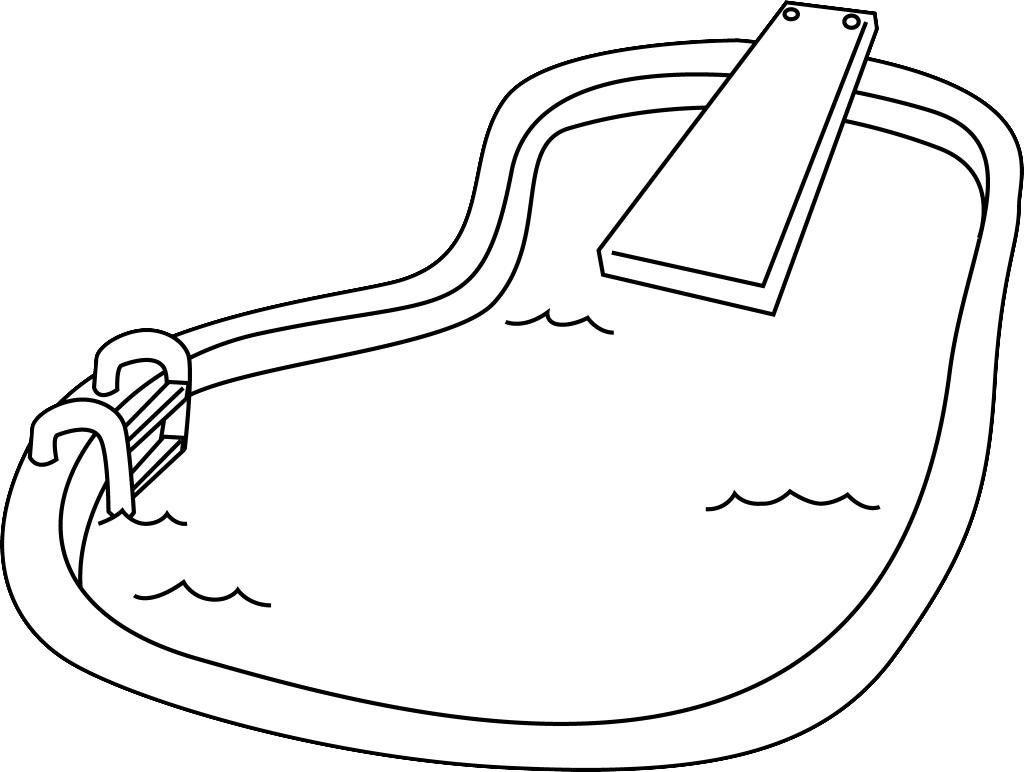
\includegraphics[width=0.4\textwidth]{figs/frontpage/smartpool.png}
\end{minipage}

\vspace{\fill}
\begin{minipage}[l]{\textwidth}
\begin{tabu} to \textwidth{lX[l]}
\textbf{Dato}           &\today\\
\textbf{Vejleder}		&Vejleder navn\\
\end{tabu}
\end{minipage}

\vspace{10pt}
\begin{minipage}[l]{\textwidth}
\tabulinesep=25pt
\begin{tabu} to \textwidth{X[l]X[l]X[l]}
 \makebox[\linewidth]{\hrulefill}\newline Joachim Dam Andersen     \newline 201370248/IKT  
&\makebox[\linewidth]{\hrulefill}\newline Lasse Priebe             \newline 201370248/IKT 
&\makebox[\linewidth]{\hrulefill}\newline Emil Nyborg              \newline 201370248/IKT\\
 \makebox[\linewidth]{\hrulefill}\newline Bjørn Nørgaard Sørensen  \newline 201370248/IKT  
&\makebox[\linewidth]{\hrulefill}\newline Alex Justesen Karlsen    \newline 201370248/IKT 
&\makebox[\linewidth]{\hrulefill}\newline Joachim Händel Noer Wind \newline 201370248/IKT
\end{tabu}
\end{minipage}\clearpage

%% Abstract
% Initial setup
\markboth{RESUMÉ/ABSTRACT}{RESUMÉ/ABSTRACT}
\abstractintoc
\abstractcol
\setlength{\abstitleskip}{-18pt}

% Abstract
\begin{abstract}
Rapporten omhandler et 3. semesterprojekt fra Ingeniørhøjskolen Aarhus Universitet udarbejdet med henblik på at producere et system, som kan fungere som dosering- og sorteringsanlæg til tabletter. Systemet er tiltænkt brug i ældreplejen, som en måde hvorpå fejlmedicinering kan undgås, og tabletsortering kan klares automatisk. Ydermere vil systemet kunne gøre personale og pårørende opmærksomme på, at brugeren ikke har afhentet sine tabletter, indenfor et givet tidsrum. Dette skal formidles ved hjælp af en Android applikation. Systemet og serveren samarbejder om at kontrollerer, hvad der dispenseres til den specifikke bruger og hvornår. Denne kommunikation er ikke fuldt ud implementeret endnu. Systemet var oprindeligt tiltænkt brug i private hjem, men undervejs i processen er idéen ændret idet at fokus flyttes fra private hjem til brug i plejesektoren. 
Produktet kan på nuværende tidspunkt dosere et bestemt antal tabletter af én enkelt type. Systemet har på nuværende tidspunkt allerede implementeret muligheden for at udvide med ekstra dispenserer, og er derfor velegnet til videreudvikling. 
Til systemet er der implementeret en fungerende brugergrænseflade, som er testet med en brugervenlighedsundersøgelse, der ved adspørgelse af 15 studerende har påpeget adskillige muligheder for forbedring.
Under systemudviklingen er den største arbejdsindsats lagt i undersøgelse af teknologier og mulige løsningsforslag.
\end{abstract}

\begin{abstracten}
The report covers a third semesterproject from the Aarhus University School of Engineering. The goal is to produce a system that can function as a dispensing and sorting machine for pills. The system is intended for use in eldercare, as a way of preventing medication errors and a way of sorting pills automaticly. Furthermore, the system will be able to notify staff and relatives if the elder has not picked up their pills, within a given timeperiod. The staff and relatives will be notified via an Android application. The system and a server operate together in order to control what is dispensed to whom and when. Though this communication is not fully implemented yet. The system was originally intended for use in private homes, but during the process, the idea evolved so that the focus was changed from home use to the healthcare sector.
The product can at this time dispense a certain number of pills which will have to be of a single type. The option of adding extra dispensers is already implemented, and is therefore suitable for further development.
The system also has a functioning interface implemented, which has been tested with a user-experience study in which 15 students participated. With the feedback made several things clear, and several of these are suitable for further work.
During the system development the largest effort was put into the study of technologies and potential solutions for the problem chosen.
\end{abstracten}\clearpage

%% Forord
\pagestyle{asereport}
\chapter{Forord}

% Forordet benyttes til at informere kort om visse ydre omstændigheder for projektet, såsom projekttype og hvor projektet er gennemført, historisk baggrund (andre arbejder, som har givet anledning til det aktuelle projekt) og hvor inspirationen og ideen er kommet fra, m.v.

Dette dokument er sammensat for at dokumentere arbejdet på 4. semesterprojektet for retningen IKT på ingeniørhøjskolen Århus.

Der vil i denne rapport være referencer til bilag og dokumentation, som det ikke ville være hensigtsmæssigt at medtage. Samtlige bilag m.m. vil være at finde på den vedlagt CD-rom. 

Source kode til projektet kan findes på CD'en. Link til vores github repo følger her: \newline \url{https://github.com/BjornNorgaard/DuckMaster3001}

\vspace{5mm}

\large{\textit{En stor tak til}}

\begin{displayquote}
    Lars Mortensen for god og brugbar vejledning.
\end{displayquote}

\begin{displayquote}
    Stjerne Apoteket for at lade gruppen komme på besøg og se deres sorteringsmaskine.
\end{displayquote}

\begin{displayquote}
    Sofie Fredslund for at lade os interviewe hende til projektet.
\end{displayquote}

\begin{displayquote}
   Underviserne på ASE, for hjælp og vejledning.
\end{displayquote}

\clearpage

%% ToC
\tableofcontents\clearpage

\mainmatter

%% Todo oversigt - SKAL UDKOMMENTERES FØR AFLEVERING
\listoftodos[Liste over gøremål]

%% Indledning
\chapter{Indledning}

Hello \cite{fysikbog} og sådan kan det jo gå.\clearpage

%% Projektformulering
\documentclass[a4paper,11pt,oneside]{memoir}
\input{utils/packages}
\input{utils/layout}
\input{utils/listings}
\input{utils/ordliste}

%% Forside variabler
\newcommand{\Kursus}{I4PRJ4 F16}
\newcommand{\Projektnavn}{SmartPool 2.0}
\newcommand{\Gruppe}{Gruppe 3}
\newcommand{\Projektdokument}{Projektrapport}

%% Litteratur
\nocite{*}
%\bibliographystyle{harvard}
\bibliography{utils/litteratur}

\begin{document}
\frontmatter

\input{utils/frontpage}\clearpage

%% Abstract
\input{docs/frontmatter/abstract}\clearpage

%% Forord
\pagestyle{asereport}
\input{docs/frontmatter/forord}\clearpage

%% ToC
\tableofcontents\clearpage

\mainmatter

%% Todo oversigt - SKAL UDKOMMENTERES FØR AFLEVERING
\listoftodos[Liste over gøremål]

%% Indledning
\input{docs/frontmatter/indledning}\clearpage

%% Projektformulering
\input{docs/projektformulering/main}\clearpage

%% Kravspecifikation
\input{docs/kravspecifikation/main}\clearpage

%% Systemarkitektur
\input{docs/systemarkitektur/main}\clearpage

%% Processbeskrivelse
\input{docs/processbeskrivelse/main}\clearpage

%% Design
\input{docs/design/main}\clearpage

%% Implementering
\input{docs/implementering/main}\clearpage

%% Integration
\input{docs/integration/main}\clearpage

%% Accepttest
\input{docs/accepttest/main}\clearpage

%% Appendix
\input{docs/appendix/main}\clearpage

\backmatter
%% Glossary
\setglossarystyle{list}
\printnoidxglossary[title=Ordliste]

% Bibliography
\clearpage
\printbibliography[title={Litteratur}]
\end{document}\clearpage

%% Kravspecifikation
\documentclass[a4paper,11pt,oneside]{memoir}
\input{utils/packages}
\input{utils/layout}
\input{utils/listings}
\input{utils/ordliste}

%% Forside variabler
\newcommand{\Kursus}{I4PRJ4 F16}
\newcommand{\Projektnavn}{SmartPool 2.0}
\newcommand{\Gruppe}{Gruppe 3}
\newcommand{\Projektdokument}{Projektrapport}

%% Litteratur
\nocite{*}
%\bibliographystyle{harvard}
\bibliography{utils/litteratur}

\begin{document}
\frontmatter

\input{utils/frontpage}\clearpage

%% Abstract
\input{docs/frontmatter/abstract}\clearpage

%% Forord
\pagestyle{asereport}
\input{docs/frontmatter/forord}\clearpage

%% ToC
\tableofcontents\clearpage

\mainmatter

%% Todo oversigt - SKAL UDKOMMENTERES FØR AFLEVERING
\listoftodos[Liste over gøremål]

%% Indledning
\input{docs/frontmatter/indledning}\clearpage

%% Projektformulering
\input{docs/projektformulering/main}\clearpage

%% Kravspecifikation
\input{docs/kravspecifikation/main}\clearpage

%% Systemarkitektur
\input{docs/systemarkitektur/main}\clearpage

%% Processbeskrivelse
\input{docs/processbeskrivelse/main}\clearpage

%% Design
\input{docs/design/main}\clearpage

%% Implementering
\input{docs/implementering/main}\clearpage

%% Integration
\input{docs/integration/main}\clearpage

%% Accepttest
\input{docs/accepttest/main}\clearpage

%% Appendix
\input{docs/appendix/main}\clearpage

\backmatter
%% Glossary
\setglossarystyle{list}
\printnoidxglossary[title=Ordliste]

% Bibliography
\clearpage
\printbibliography[title={Litteratur}]
\end{document}\clearpage

%% Systemarkitektur
\documentclass[a4paper,11pt,oneside]{memoir}
\input{utils/packages}
\input{utils/layout}
\input{utils/listings}
\input{utils/ordliste}

%% Forside variabler
\newcommand{\Kursus}{I4PRJ4 F16}
\newcommand{\Projektnavn}{SmartPool 2.0}
\newcommand{\Gruppe}{Gruppe 3}
\newcommand{\Projektdokument}{Projektrapport}

%% Litteratur
\nocite{*}
%\bibliographystyle{harvard}
\bibliography{utils/litteratur}

\begin{document}
\frontmatter

\input{utils/frontpage}\clearpage

%% Abstract
\input{docs/frontmatter/abstract}\clearpage

%% Forord
\pagestyle{asereport}
\input{docs/frontmatter/forord}\clearpage

%% ToC
\tableofcontents\clearpage

\mainmatter

%% Todo oversigt - SKAL UDKOMMENTERES FØR AFLEVERING
\listoftodos[Liste over gøremål]

%% Indledning
\input{docs/frontmatter/indledning}\clearpage

%% Projektformulering
\input{docs/projektformulering/main}\clearpage

%% Kravspecifikation
\input{docs/kravspecifikation/main}\clearpage

%% Systemarkitektur
\input{docs/systemarkitektur/main}\clearpage

%% Processbeskrivelse
\input{docs/processbeskrivelse/main}\clearpage

%% Design
\input{docs/design/main}\clearpage

%% Implementering
\input{docs/implementering/main}\clearpage

%% Integration
\input{docs/integration/main}\clearpage

%% Accepttest
\input{docs/accepttest/main}\clearpage

%% Appendix
\input{docs/appendix/main}\clearpage

\backmatter
%% Glossary
\setglossarystyle{list}
\printnoidxglossary[title=Ordliste]

% Bibliography
\clearpage
\printbibliography[title={Litteratur}]
\end{document}\clearpage

%% Processbeskrivelse
\documentclass[a4paper,11pt,oneside]{memoir}
\input{utils/packages}
\input{utils/layout}
\input{utils/listings}
\input{utils/ordliste}

%% Forside variabler
\newcommand{\Kursus}{I4PRJ4 F16}
\newcommand{\Projektnavn}{SmartPool 2.0}
\newcommand{\Gruppe}{Gruppe 3}
\newcommand{\Projektdokument}{Projektrapport}

%% Litteratur
\nocite{*}
%\bibliographystyle{harvard}
\bibliography{utils/litteratur}

\begin{document}
\frontmatter

\input{utils/frontpage}\clearpage

%% Abstract
\input{docs/frontmatter/abstract}\clearpage

%% Forord
\pagestyle{asereport}
\input{docs/frontmatter/forord}\clearpage

%% ToC
\tableofcontents\clearpage

\mainmatter

%% Todo oversigt - SKAL UDKOMMENTERES FØR AFLEVERING
\listoftodos[Liste over gøremål]

%% Indledning
\input{docs/frontmatter/indledning}\clearpage

%% Projektformulering
\input{docs/projektformulering/main}\clearpage

%% Kravspecifikation
\input{docs/kravspecifikation/main}\clearpage

%% Systemarkitektur
\input{docs/systemarkitektur/main}\clearpage

%% Processbeskrivelse
\input{docs/processbeskrivelse/main}\clearpage

%% Design
\input{docs/design/main}\clearpage

%% Implementering
\input{docs/implementering/main}\clearpage

%% Integration
\input{docs/integration/main}\clearpage

%% Accepttest
\input{docs/accepttest/main}\clearpage

%% Appendix
\input{docs/appendix/main}\clearpage

\backmatter
%% Glossary
\setglossarystyle{list}
\printnoidxglossary[title=Ordliste]

% Bibliography
\clearpage
\printbibliography[title={Litteratur}]
\end{document}\clearpage

%% Design
\documentclass[a4paper,11pt,oneside]{memoir}
\input{utils/packages}
\input{utils/layout}
\input{utils/listings}
\input{utils/ordliste}

%% Forside variabler
\newcommand{\Kursus}{I4PRJ4 F16}
\newcommand{\Projektnavn}{SmartPool 2.0}
\newcommand{\Gruppe}{Gruppe 3}
\newcommand{\Projektdokument}{Projektrapport}

%% Litteratur
\nocite{*}
%\bibliographystyle{harvard}
\bibliography{utils/litteratur}

\begin{document}
\frontmatter

\input{utils/frontpage}\clearpage

%% Abstract
\input{docs/frontmatter/abstract}\clearpage

%% Forord
\pagestyle{asereport}
\input{docs/frontmatter/forord}\clearpage

%% ToC
\tableofcontents\clearpage

\mainmatter

%% Todo oversigt - SKAL UDKOMMENTERES FØR AFLEVERING
\listoftodos[Liste over gøremål]

%% Indledning
\input{docs/frontmatter/indledning}\clearpage

%% Projektformulering
\input{docs/projektformulering/main}\clearpage

%% Kravspecifikation
\input{docs/kravspecifikation/main}\clearpage

%% Systemarkitektur
\input{docs/systemarkitektur/main}\clearpage

%% Processbeskrivelse
\input{docs/processbeskrivelse/main}\clearpage

%% Design
\input{docs/design/main}\clearpage

%% Implementering
\input{docs/implementering/main}\clearpage

%% Integration
\input{docs/integration/main}\clearpage

%% Accepttest
\input{docs/accepttest/main}\clearpage

%% Appendix
\input{docs/appendix/main}\clearpage

\backmatter
%% Glossary
\setglossarystyle{list}
\printnoidxglossary[title=Ordliste]

% Bibliography
\clearpage
\printbibliography[title={Litteratur}]
\end{document}\clearpage

%% Implementering
\documentclass[a4paper,11pt,oneside]{memoir}
\input{utils/packages}
\input{utils/layout}
\input{utils/listings}
\input{utils/ordliste}

%% Forside variabler
\newcommand{\Kursus}{I4PRJ4 F16}
\newcommand{\Projektnavn}{SmartPool 2.0}
\newcommand{\Gruppe}{Gruppe 3}
\newcommand{\Projektdokument}{Projektrapport}

%% Litteratur
\nocite{*}
%\bibliographystyle{harvard}
\bibliography{utils/litteratur}

\begin{document}
\frontmatter

\input{utils/frontpage}\clearpage

%% Abstract
\input{docs/frontmatter/abstract}\clearpage

%% Forord
\pagestyle{asereport}
\input{docs/frontmatter/forord}\clearpage

%% ToC
\tableofcontents\clearpage

\mainmatter

%% Todo oversigt - SKAL UDKOMMENTERES FØR AFLEVERING
\listoftodos[Liste over gøremål]

%% Indledning
\input{docs/frontmatter/indledning}\clearpage

%% Projektformulering
\input{docs/projektformulering/main}\clearpage

%% Kravspecifikation
\input{docs/kravspecifikation/main}\clearpage

%% Systemarkitektur
\input{docs/systemarkitektur/main}\clearpage

%% Processbeskrivelse
\input{docs/processbeskrivelse/main}\clearpage

%% Design
\input{docs/design/main}\clearpage

%% Implementering
\input{docs/implementering/main}\clearpage

%% Integration
\input{docs/integration/main}\clearpage

%% Accepttest
\input{docs/accepttest/main}\clearpage

%% Appendix
\input{docs/appendix/main}\clearpage

\backmatter
%% Glossary
\setglossarystyle{list}
\printnoidxglossary[title=Ordliste]

% Bibliography
\clearpage
\printbibliography[title={Litteratur}]
\end{document}\clearpage

%% Integration
\documentclass[a4paper,11pt,oneside]{memoir}
\input{utils/packages}
\input{utils/layout}
\input{utils/listings}
\input{utils/ordliste}

%% Forside variabler
\newcommand{\Kursus}{I4PRJ4 F16}
\newcommand{\Projektnavn}{SmartPool 2.0}
\newcommand{\Gruppe}{Gruppe 3}
\newcommand{\Projektdokument}{Projektrapport}

%% Litteratur
\nocite{*}
%\bibliographystyle{harvard}
\bibliography{utils/litteratur}

\begin{document}
\frontmatter

\input{utils/frontpage}\clearpage

%% Abstract
\input{docs/frontmatter/abstract}\clearpage

%% Forord
\pagestyle{asereport}
\input{docs/frontmatter/forord}\clearpage

%% ToC
\tableofcontents\clearpage

\mainmatter

%% Todo oversigt - SKAL UDKOMMENTERES FØR AFLEVERING
\listoftodos[Liste over gøremål]

%% Indledning
\input{docs/frontmatter/indledning}\clearpage

%% Projektformulering
\input{docs/projektformulering/main}\clearpage

%% Kravspecifikation
\input{docs/kravspecifikation/main}\clearpage

%% Systemarkitektur
\input{docs/systemarkitektur/main}\clearpage

%% Processbeskrivelse
\input{docs/processbeskrivelse/main}\clearpage

%% Design
\input{docs/design/main}\clearpage

%% Implementering
\input{docs/implementering/main}\clearpage

%% Integration
\input{docs/integration/main}\clearpage

%% Accepttest
\input{docs/accepttest/main}\clearpage

%% Appendix
\input{docs/appendix/main}\clearpage

\backmatter
%% Glossary
\setglossarystyle{list}
\printnoidxglossary[title=Ordliste]

% Bibliography
\clearpage
\printbibliography[title={Litteratur}]
\end{document}\clearpage

%% Accepttest
\documentclass[a4paper,11pt,oneside]{memoir}
\input{utils/packages}
\input{utils/layout}
\input{utils/listings}
\input{utils/ordliste}

%% Forside variabler
\newcommand{\Kursus}{I4PRJ4 F16}
\newcommand{\Projektnavn}{SmartPool 2.0}
\newcommand{\Gruppe}{Gruppe 3}
\newcommand{\Projektdokument}{Projektrapport}

%% Litteratur
\nocite{*}
%\bibliographystyle{harvard}
\bibliography{utils/litteratur}

\begin{document}
\frontmatter

\input{utils/frontpage}\clearpage

%% Abstract
\input{docs/frontmatter/abstract}\clearpage

%% Forord
\pagestyle{asereport}
\input{docs/frontmatter/forord}\clearpage

%% ToC
\tableofcontents\clearpage

\mainmatter

%% Todo oversigt - SKAL UDKOMMENTERES FØR AFLEVERING
\listoftodos[Liste over gøremål]

%% Indledning
\input{docs/frontmatter/indledning}\clearpage

%% Projektformulering
\input{docs/projektformulering/main}\clearpage

%% Kravspecifikation
\input{docs/kravspecifikation/main}\clearpage

%% Systemarkitektur
\input{docs/systemarkitektur/main}\clearpage

%% Processbeskrivelse
\input{docs/processbeskrivelse/main}\clearpage

%% Design
\input{docs/design/main}\clearpage

%% Implementering
\input{docs/implementering/main}\clearpage

%% Integration
\input{docs/integration/main}\clearpage

%% Accepttest
\input{docs/accepttest/main}\clearpage

%% Appendix
\input{docs/appendix/main}\clearpage

\backmatter
%% Glossary
\setglossarystyle{list}
\printnoidxglossary[title=Ordliste]

% Bibliography
\clearpage
\printbibliography[title={Litteratur}]
\end{document}\clearpage

%% Appendix
\documentclass[a4paper,11pt,oneside]{memoir}
\input{utils/packages}
\input{utils/layout}
\input{utils/listings}
\input{utils/ordliste}

%% Forside variabler
\newcommand{\Kursus}{I4PRJ4 F16}
\newcommand{\Projektnavn}{SmartPool 2.0}
\newcommand{\Gruppe}{Gruppe 3}
\newcommand{\Projektdokument}{Projektrapport}

%% Litteratur
\nocite{*}
%\bibliographystyle{harvard}
\bibliography{utils/litteratur}

\begin{document}
\frontmatter

\input{utils/frontpage}\clearpage

%% Abstract
\input{docs/frontmatter/abstract}\clearpage

%% Forord
\pagestyle{asereport}
\input{docs/frontmatter/forord}\clearpage

%% ToC
\tableofcontents\clearpage

\mainmatter

%% Todo oversigt - SKAL UDKOMMENTERES FØR AFLEVERING
\listoftodos[Liste over gøremål]

%% Indledning
\input{docs/frontmatter/indledning}\clearpage

%% Projektformulering
\input{docs/projektformulering/main}\clearpage

%% Kravspecifikation
\input{docs/kravspecifikation/main}\clearpage

%% Systemarkitektur
\input{docs/systemarkitektur/main}\clearpage

%% Processbeskrivelse
\input{docs/processbeskrivelse/main}\clearpage

%% Design
\input{docs/design/main}\clearpage

%% Implementering
\input{docs/implementering/main}\clearpage

%% Integration
\input{docs/integration/main}\clearpage

%% Accepttest
\input{docs/accepttest/main}\clearpage

%% Appendix
\input{docs/appendix/main}\clearpage

\backmatter
%% Glossary
\setglossarystyle{list}
\printnoidxglossary[title=Ordliste]

% Bibliography
\clearpage
\printbibliography[title={Litteratur}]
\end{document}\clearpage

\backmatter
%% Glossary
\setglossarystyle{list}
\printnoidxglossary[title=Ordliste]

% Bibliography
\clearpage
\printbibliography[title={Litteratur}]
\end{document}\clearpage

%% Systemarkitektur
\documentclass[a4paper,11pt,oneside]{memoir}
%!TEX root = main.tex
% Encoding
%\usepackage[utf8]{inputenc} % pdfLatex
\usepackage[T1]{fontenc}
\usepackage[danish]{babel}
\renewcommand{\danishhyphenmins}{22}
\usepackage[utf8]{inputenc} % æ ø å

% Date
\usepackage[ddmmyyyy]{datetime}
\renewcommand{\dateseparator}{.}

% Fonts
\usepackage{fourier}
\usepackage[scaled=0.8]{beramono}

% Math
\usepackage{amsmath,amssymb}
\usepackage{bm}
\usepackage{amsthm}
\usepackage{mathtools}

% Graphics
\usepackage[usenames,dvipsnames,table]{xcolor}
\usepackage{graphicx}
\usepackage{float}
%\usepackage[section]{placeins}
\usepackage{tikz}
\usepackage[pages=some]{background}
\usepackage{wrapfig}

% Listings & Tables
\usepackage{listings}
%\usepackage{pythontex}
\usepackage{enumitem}
\usepackage{tabu}
\usepackage{longtable}
\usepackage{multirow}
\usepackage{makecell}


% References & Quotes
%\usepackage[danish]{varioref}				% Muliggoer bl.a. krydshenvisninger med sidetal (\vref)
%\usepackage{nat}							% Udvidelse med naturvidenskabelige citationsmodeller
\usepackage[danish=guillemets]{csquotes}
\usepackage[hidelinks]{hyperref}
\hypersetup{
    pdfstartview={FitH},
    pdftitle={Smart Pool 2.0},
    pdfsubject={Projektrapport},
    pdfauthor={I4PRJ4GRP3}
}
\usepackage[all]{hypcap}

% Etc
\usepackage[
	%backend=biber,
	backend=bibtex,
	style=ieee,
	natbib=true,
	backref=false,
	backrefstyle=all+,
	hyperref=true
]{biblatex}
\usepackage{pdflscape}
\usepackage[nomain,toc,xindy,acronym,nonumberlist,noredefwarn]{glossaries}
\usepackage[xindy]{imakeidx}
\usepackage{float}
\makeindex

% Dummy
\usepackage{lipsum}
%!TEX root = main.tex
% Page setup
\setulmarginsandblock{35mm}{25mm}{*}
\setlrmarginsandblock{20mm}{20mm}{*}
\setheadfoot{4\onelineskip}{2\onelineskip}
\setheaderspaces{*}{5mm}{*}
\checkandfixthelayout

% Pagestyle
\makepagestyle{asereport}
	\makeevenhead{asereport}{}{}{}
	\makeoddhead{asereport}{
\includegraphics{figs/frontpage/aseaulogo.pdf}}{}{\small\rightmark{} | \textbf{\thepage{}\vspace{7pt}}}
	\makeevenfoot{asereport}{}{}{}
	\makeoddfoot{asereport}{}{}{}

\makepsmarks{asereport}{
	\createmark{chapter}{both}{shownumber}{}{. \ }
	\createmark{section}{both}{shownumber}{}{. \ }
	\createmark{subsection}{both}{shownumber}{}{. \ }
	\createplainmark{toc}{both}{\contentsname}
	\createplainmark{lof}{both}{\listfigurename}
	\createplainmark{lot}{both}{\listtablename}
	\createplainmark{bib}{both}{\bibname}
	\createplainmark{index}{both}{\indexname}
	\createplainmark{glossary}{both}{\glossaryname}
}

\aliaspagestyle{part}{asereport}
\aliaspagestyle{chapter}{asereport}
\chapterstyle{tandh}

% Modification to certain spacing
\setlength{\parskip}{8pt}
\setlength{\parindent}{0pt}
\setlength{\abovecaptionskip}{7pt}
\setlength{\belowcaptionskip}{-10pt}
\OnehalfSpacing

% Tabu
%\taburowcolors[1]2{white .. light-gray}
\tabulinesep=4pt

% Itemize/enumerate
\setlist{
    before=\vspace{-3pt}, 
    after=\vspace{-3pt},
    itemsep=0pt,
    leftmargin=25pt,
    labelsep=10pt,
    topsep=0pt,
}

% Kommandoer til UC - fixer spacing
% Aktører
\newcommand{\fua}[1]{
	\begin{minipage}[t]{\linewidth}
		\setlist{
		    leftmargin=22pt,
		    itemsep=0pt,
		    topsep=0pt,
		    parsep=3pt
		}
	\begin{itemize}[before={\vspace{-6pt}}, after={\vspace{6pt}}]
	#1
	\end{itemize}
	\end{minipage}
}

% Hovedforløb
\newcommand{\fu}[1]{
\begin{minipage}[t]{\linewidth}
\setlist{
    leftmargin=22pt,
    itemsep=0pt,
    topsep=0pt,
    parsep=3pt
}
\raggedright
\begin{enumerate}[before={\vspace{-5pt}},after={\vspace{6pt}}]
#1
\end{enumerate}
\end{minipage}}

% Extensions
\newcommand{\fuex}[2]{
\begin{minipage}[t]{\linewidth}
\vspace{-6pt}
\raggedright
\textit{#1}
\begin{enumerate}[leftmargin=22pt,itemsep=0pt,parsep=3pt,before={\vspace{-8pt}}, after={\vspace{20pt}},topsep=8pt]
#2
\end{enumerate}
\end{minipage}
}

% Extensions - Sidste entry
\newcommand{\fuexl}[2]{
\begin{minipage}[t]{\linewidth}
\vspace{-6pt}
\raggedright
\textit{#1}
\begin{enumerate}[leftmargin=22pt,itemsep=0pt,parsep=3pt,before={\vspace{-8pt}}, after={\vspace{3pt}},topsep=8pt]
#2
\end{enumerate}
\end{minipage}}

% Versionshistorik
\newcommand{\verhistitem}[2]{
\begin{minipage}[t]{\linewidth}
\vspace{-6pt}
\raggedright
#1
\begin{itemize}[leftmargin=22pt,itemsep=0pt,parsep=0pt,before={\vspace{-10pt}},after={\vspace{3pt}},topsep=8pt]
#2
\end{itemize}
\end{minipage}}

\newcommand{\tverb}[1]{{\texttt{#1}}}

\newcommand{\cond}[1]{
\begin{itemize}[label=,noitemsep,topsep=0pt,after={\vspace*{-\baselineskip}}]
#1
\end{itemize}}

% Etc
\definecolor{light-gray}{gray}{0.8}
\definecolor{pantone}{RGB}{0,61,133}

\setfloatlocations{figure}{H}
\setfloatlocations{table}{H}

\numberwithin{equation}{chapter}
\numberwithin{figure}{chapter}
\setcounter{secnumdepth}{3}
\setcounter{tocdepth}{2}
\maxsecnumdepth{subsection}

\renewcommand*{\cftdotsep}{1}
\setpnumwidth{2em}
\setrmarg{2em}

\setverbatimfont{\ttfamily}

%\renewcommand\cftchaptername {\chaptername~}
%\renewcommand\cftappendixname {\appendixname~}
\addto\captionsdanish{
    \renewcommand\contentsname{Indholdsfortegnelse}
    \renewcommand\appendixname{Appendiks}
}
\renewcommand\appendixpagename{Appendiks}
\renewcommand\appendixtocname{Appendiks}
\newsubfloat{figure}

% Abstract
\newenvironment{abstracten}
{\renewcommand{\abstractname}{Abstract}\abstract}
{\endabstract}
\renewcommand{\abstractnamefont}{\normalfont\Large\bfseries}
%!TEX root = main.tex
% Listings
\AtBeginDocument{%
  \counterwithin*{lstlisting}{section}
  \counterwithin*{lstlisting}{subsection}
  \counterwithin*{lstlisting}{subsubsection}
  \renewcommand{\thelstlisting}{%
    \ifnum\value{subsection}=0
      \thesection.\arabic{lstlisting}%
    \else
      \ifnum\value{subsubsection}=0
        \thesubsection.\arabic{lstlisting}%
      \else
        \thesubsubsection.\arabic{lstlisting}%
      \fi
    \fi
  }
}

% Loading languages
\lstloadlanguages{C, C++}

% Listing setup
\lstdefinestyle{all}{
    basicstyle    = \ttfamily\SingleSpacing\scriptsize,
    numbers       = left, 
    numberstyle   = \ttfamily\tiny,
    breaklines    = true,
    commentstyle=\color{green},
    %backgroundcolor = \color{red},
    numbersep     = 20pt,
    xleftmargin   = \parindent,
    captionpos    = b,
    keywordstyle  = [1]\color{Blue}\bfseries,
    commentstyle  = \itshape\color{Green},
    tabsize       = 3
}

\lstset{
    style = all
} 
%!TEX root = main.tex
\makenoidxglossaries
\newglossaryentry{gui}{
    name={GUI}, 
    description={Graphical User Interface er en brugergrænseflade. Brugerens måde at tilgå systemet på}}

\newglossaryentry{psoc}{
    name={PSoC}, 
    description={PSoC (Programmable System-on-Chip) er et microcontroller system produceret af Cypress Semiconductor}}

\newglossaryentry{moscow}{
    name={MoSCoW}, 
    description={MoSCoW er en metode til at prioritere krav til ens system}}

\newglossaryentry{furps}{
    name={FURPS}, 
    description={FURPS er en metode til kategorisering af systemets ikke-funktionelle krav}}

\newglossaryentry{BDD}{
    name={BDD}, 
    description={BDD (Block Definition Diagram) er et diagram, som beskriver et system ved at opdele det op i mindre blokke}}

\newglossaryentry{IBD}{
    name={IBD}, 
    description={IBD (Internal Block Diagram) er et diagram, som viser forbindelserne mellem blokkene, som kan findes i et BDD}}

\newglossaryentry{pilleskuffe}{
    name={Pilleskuffe},
    description={Skuffen under dispenseren, hvor i den nederste pille ligger i. Skuffen tømmes ved at elektromagneten trækker skuffen til sig.}}

\newglossaryentry{pilledispenser}{
    name={Pilledispenser},
    description={Det rør som pillerne bliver opbevaret i.}}

\newglossaryentry{elektromagneten}{
    name={Elektromagneten},
    description={Elektromagneten er en spole der sendes strøm igennem. Når der er strøm på spolen dannes et magnetfelt. Der vil ofte være tale om det samme hvad enten der står spole eller elektromagnet.}}

%% Forside variabler
\newcommand{\Kursus}{I4PRJ4 F16}
\newcommand{\Projektnavn}{SmartPool 2.0}
\newcommand{\Gruppe}{Gruppe 3}
\newcommand{\Projektdokument}{Projektrapport}

%% Litteratur
\nocite{*}
%\bibliographystyle{harvard}
\bibliography{utils/litteratur}

\begin{document}
\frontmatter

%!TEX root = main.tex
\pagestyle{titlingpage}
\backgroundsetup{
	scale=1,
	angle=0,
	opacity=1,
	contents={
		\begin{tikzpicture}[remember picture,overlay]
		\path [fill=pantone] (-0.5\paperwidth,0.36\paperheight) rectangle (0.5\paperwidth,0.47\paperheight);  
		\path [fill=pantone] (-0.5\paperwidth,-0.47\paperheight) rectangle (0.5\paperwidth,-0.43\paperheight);  
		\end{tikzpicture}}}
\BgThispage
\vspace*{-25mm}
\begin{minipage}[l]{\textwidth}
	
\includegraphics[width=0.75\textwidth]{figs/frontpage/aseaulogohvid.pdf}
\end{minipage}

\vspace{35pt}
\begin{minipage}[l]{\textwidth}
\tabulinesep=10pt
\begin{tabu} to \textwidth{X[l]}
	{\small\MakeUppercase\Kursus}\\
	{\HUGE\bfseries\MakeUppercase\Projektnavn}\\
	{\Large\Gruppe}\\
	{\itshape\Projektdokument}
\end{tabu}
\end{minipage}

\vspace{5pt}
\begin{minipage}[l]{\textwidth}
    \centering
	\vspace*{0cm}\hspace*{8cm}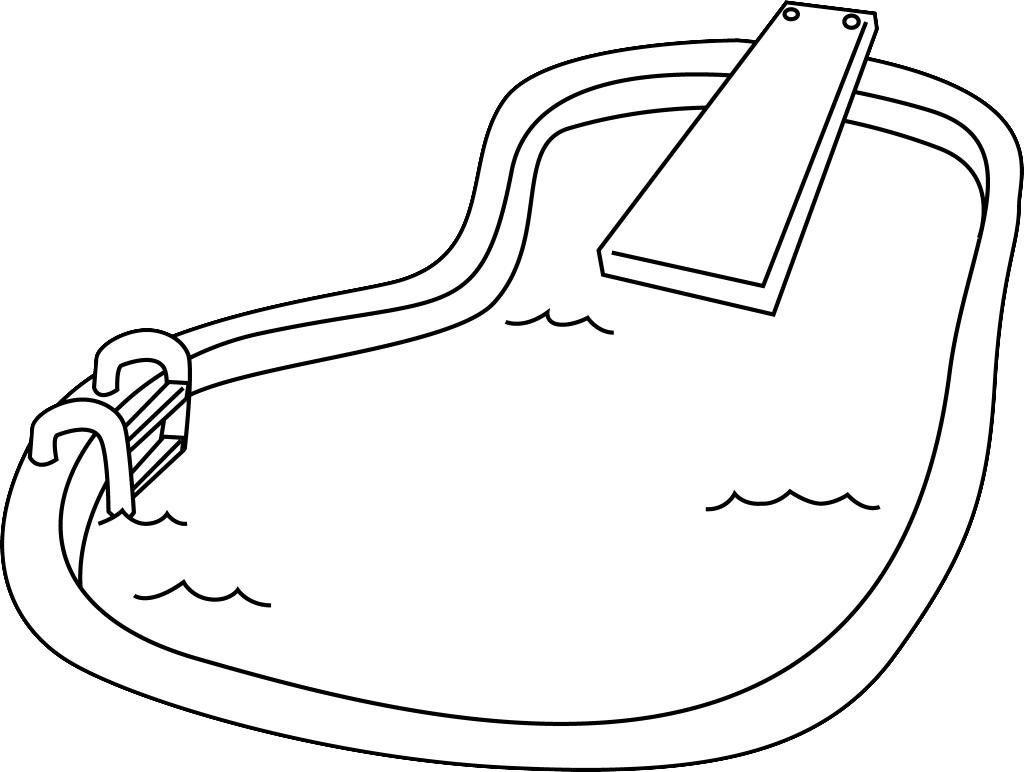
\includegraphics[width=0.4\textwidth]{figs/frontpage/smartpool.png}
\end{minipage}

\vspace{\fill}
\begin{minipage}[l]{\textwidth}
\begin{tabu} to \textwidth{lX[l]}
\textbf{Dato}           &\today\\
\textbf{Vejleder}		&Vejleder navn\\
\end{tabu}
\end{minipage}

\vspace{10pt}
\begin{minipage}[l]{\textwidth}
\tabulinesep=25pt
\begin{tabu} to \textwidth{X[l]X[l]X[l]}
 \makebox[\linewidth]{\hrulefill}\newline Joachim Dam Andersen     \newline 201370248/IKT  
&\makebox[\linewidth]{\hrulefill}\newline Lasse Priebe             \newline 201370248/IKT 
&\makebox[\linewidth]{\hrulefill}\newline Emil Nyborg              \newline 201370248/IKT\\
 \makebox[\linewidth]{\hrulefill}\newline Bjørn Nørgaard Sørensen  \newline 201370248/IKT  
&\makebox[\linewidth]{\hrulefill}\newline Alex Justesen Karlsen    \newline 201370248/IKT 
&\makebox[\linewidth]{\hrulefill}\newline Joachim Händel Noer Wind \newline 201370248/IKT
\end{tabu}
\end{minipage}\clearpage

%% Abstract
% Initial setup
\markboth{RESUMÉ/ABSTRACT}{RESUMÉ/ABSTRACT}
\abstractintoc
\abstractcol
\setlength{\abstitleskip}{-18pt}

% Abstract
\begin{abstract}
Rapporten omhandler et 3. semesterprojekt fra Ingeniørhøjskolen Aarhus Universitet udarbejdet med henblik på at producere et system, som kan fungere som dosering- og sorteringsanlæg til tabletter. Systemet er tiltænkt brug i ældreplejen, som en måde hvorpå fejlmedicinering kan undgås, og tabletsortering kan klares automatisk. Ydermere vil systemet kunne gøre personale og pårørende opmærksomme på, at brugeren ikke har afhentet sine tabletter, indenfor et givet tidsrum. Dette skal formidles ved hjælp af en Android applikation. Systemet og serveren samarbejder om at kontrollerer, hvad der dispenseres til den specifikke bruger og hvornår. Denne kommunikation er ikke fuldt ud implementeret endnu. Systemet var oprindeligt tiltænkt brug i private hjem, men undervejs i processen er idéen ændret idet at fokus flyttes fra private hjem til brug i plejesektoren. 
Produktet kan på nuværende tidspunkt dosere et bestemt antal tabletter af én enkelt type. Systemet har på nuværende tidspunkt allerede implementeret muligheden for at udvide med ekstra dispenserer, og er derfor velegnet til videreudvikling. 
Til systemet er der implementeret en fungerende brugergrænseflade, som er testet med en brugervenlighedsundersøgelse, der ved adspørgelse af 15 studerende har påpeget adskillige muligheder for forbedring.
Under systemudviklingen er den største arbejdsindsats lagt i undersøgelse af teknologier og mulige løsningsforslag.
\end{abstract}

\begin{abstracten}
The report covers a third semesterproject from the Aarhus University School of Engineering. The goal is to produce a system that can function as a dispensing and sorting machine for pills. The system is intended for use in eldercare, as a way of preventing medication errors and a way of sorting pills automaticly. Furthermore, the system will be able to notify staff and relatives if the elder has not picked up their pills, within a given timeperiod. The staff and relatives will be notified via an Android application. The system and a server operate together in order to control what is dispensed to whom and when. Though this communication is not fully implemented yet. The system was originally intended for use in private homes, but during the process, the idea evolved so that the focus was changed from home use to the healthcare sector.
The product can at this time dispense a certain number of pills which will have to be of a single type. The option of adding extra dispensers is already implemented, and is therefore suitable for further development.
The system also has a functioning interface implemented, which has been tested with a user-experience study in which 15 students participated. With the feedback made several things clear, and several of these are suitable for further work.
During the system development the largest effort was put into the study of technologies and potential solutions for the problem chosen.
\end{abstracten}\clearpage

%% Forord
\pagestyle{asereport}
\chapter{Forord}

% Forordet benyttes til at informere kort om visse ydre omstændigheder for projektet, såsom projekttype og hvor projektet er gennemført, historisk baggrund (andre arbejder, som har givet anledning til det aktuelle projekt) og hvor inspirationen og ideen er kommet fra, m.v.

Dette dokument er sammensat for at dokumentere arbejdet på 4. semesterprojektet for retningen IKT på ingeniørhøjskolen Århus.

Der vil i denne rapport være referencer til bilag og dokumentation, som det ikke ville være hensigtsmæssigt at medtage. Samtlige bilag m.m. vil være at finde på den vedlagt CD-rom. 

Source kode til projektet kan findes på CD'en. Link til vores github repo følger her: \newline \url{https://github.com/BjornNorgaard/DuckMaster3001}

\vspace{5mm}

\large{\textit{En stor tak til}}

\begin{displayquote}
    Lars Mortensen for god og brugbar vejledning.
\end{displayquote}

\begin{displayquote}
    Stjerne Apoteket for at lade gruppen komme på besøg og se deres sorteringsmaskine.
\end{displayquote}

\begin{displayquote}
    Sofie Fredslund for at lade os interviewe hende til projektet.
\end{displayquote}

\begin{displayquote}
   Underviserne på ASE, for hjælp og vejledning.
\end{displayquote}

\clearpage

%% ToC
\tableofcontents\clearpage

\mainmatter

%% Todo oversigt - SKAL UDKOMMENTERES FØR AFLEVERING
\listoftodos[Liste over gøremål]

%% Indledning
\chapter{Indledning}

Hello \cite{fysikbog} og sådan kan det jo gå.\clearpage

%% Projektformulering
\documentclass[a4paper,11pt,oneside]{memoir}
\input{utils/packages}
\input{utils/layout}
\input{utils/listings}
\input{utils/ordliste}

%% Forside variabler
\newcommand{\Kursus}{I4PRJ4 F16}
\newcommand{\Projektnavn}{SmartPool 2.0}
\newcommand{\Gruppe}{Gruppe 3}
\newcommand{\Projektdokument}{Projektrapport}

%% Litteratur
\nocite{*}
%\bibliographystyle{harvard}
\bibliography{utils/litteratur}

\begin{document}
\frontmatter

\input{utils/frontpage}\clearpage

%% Abstract
\input{docs/frontmatter/abstract}\clearpage

%% Forord
\pagestyle{asereport}
\input{docs/frontmatter/forord}\clearpage

%% ToC
\tableofcontents\clearpage

\mainmatter

%% Todo oversigt - SKAL UDKOMMENTERES FØR AFLEVERING
\listoftodos[Liste over gøremål]

%% Indledning
\input{docs/frontmatter/indledning}\clearpage

%% Projektformulering
\input{docs/projektformulering/main}\clearpage

%% Kravspecifikation
\input{docs/kravspecifikation/main}\clearpage

%% Systemarkitektur
\input{docs/systemarkitektur/main}\clearpage

%% Processbeskrivelse
\input{docs/processbeskrivelse/main}\clearpage

%% Design
\input{docs/design/main}\clearpage

%% Implementering
\input{docs/implementering/main}\clearpage

%% Integration
\input{docs/integration/main}\clearpage

%% Accepttest
\input{docs/accepttest/main}\clearpage

%% Appendix
\input{docs/appendix/main}\clearpage

\backmatter
%% Glossary
\setglossarystyle{list}
\printnoidxglossary[title=Ordliste]

% Bibliography
\clearpage
\printbibliography[title={Litteratur}]
\end{document}\clearpage

%% Kravspecifikation
\documentclass[a4paper,11pt,oneside]{memoir}
\input{utils/packages}
\input{utils/layout}
\input{utils/listings}
\input{utils/ordliste}

%% Forside variabler
\newcommand{\Kursus}{I4PRJ4 F16}
\newcommand{\Projektnavn}{SmartPool 2.0}
\newcommand{\Gruppe}{Gruppe 3}
\newcommand{\Projektdokument}{Projektrapport}

%% Litteratur
\nocite{*}
%\bibliographystyle{harvard}
\bibliography{utils/litteratur}

\begin{document}
\frontmatter

\input{utils/frontpage}\clearpage

%% Abstract
\input{docs/frontmatter/abstract}\clearpage

%% Forord
\pagestyle{asereport}
\input{docs/frontmatter/forord}\clearpage

%% ToC
\tableofcontents\clearpage

\mainmatter

%% Todo oversigt - SKAL UDKOMMENTERES FØR AFLEVERING
\listoftodos[Liste over gøremål]

%% Indledning
\input{docs/frontmatter/indledning}\clearpage

%% Projektformulering
\input{docs/projektformulering/main}\clearpage

%% Kravspecifikation
\input{docs/kravspecifikation/main}\clearpage

%% Systemarkitektur
\input{docs/systemarkitektur/main}\clearpage

%% Processbeskrivelse
\input{docs/processbeskrivelse/main}\clearpage

%% Design
\input{docs/design/main}\clearpage

%% Implementering
\input{docs/implementering/main}\clearpage

%% Integration
\input{docs/integration/main}\clearpage

%% Accepttest
\input{docs/accepttest/main}\clearpage

%% Appendix
\input{docs/appendix/main}\clearpage

\backmatter
%% Glossary
\setglossarystyle{list}
\printnoidxglossary[title=Ordliste]

% Bibliography
\clearpage
\printbibliography[title={Litteratur}]
\end{document}\clearpage

%% Systemarkitektur
\documentclass[a4paper,11pt,oneside]{memoir}
\input{utils/packages}
\input{utils/layout}
\input{utils/listings}
\input{utils/ordliste}

%% Forside variabler
\newcommand{\Kursus}{I4PRJ4 F16}
\newcommand{\Projektnavn}{SmartPool 2.0}
\newcommand{\Gruppe}{Gruppe 3}
\newcommand{\Projektdokument}{Projektrapport}

%% Litteratur
\nocite{*}
%\bibliographystyle{harvard}
\bibliography{utils/litteratur}

\begin{document}
\frontmatter

\input{utils/frontpage}\clearpage

%% Abstract
\input{docs/frontmatter/abstract}\clearpage

%% Forord
\pagestyle{asereport}
\input{docs/frontmatter/forord}\clearpage

%% ToC
\tableofcontents\clearpage

\mainmatter

%% Todo oversigt - SKAL UDKOMMENTERES FØR AFLEVERING
\listoftodos[Liste over gøremål]

%% Indledning
\input{docs/frontmatter/indledning}\clearpage

%% Projektformulering
\input{docs/projektformulering/main}\clearpage

%% Kravspecifikation
\input{docs/kravspecifikation/main}\clearpage

%% Systemarkitektur
\input{docs/systemarkitektur/main}\clearpage

%% Processbeskrivelse
\input{docs/processbeskrivelse/main}\clearpage

%% Design
\input{docs/design/main}\clearpage

%% Implementering
\input{docs/implementering/main}\clearpage

%% Integration
\input{docs/integration/main}\clearpage

%% Accepttest
\input{docs/accepttest/main}\clearpage

%% Appendix
\input{docs/appendix/main}\clearpage

\backmatter
%% Glossary
\setglossarystyle{list}
\printnoidxglossary[title=Ordliste]

% Bibliography
\clearpage
\printbibliography[title={Litteratur}]
\end{document}\clearpage

%% Processbeskrivelse
\documentclass[a4paper,11pt,oneside]{memoir}
\input{utils/packages}
\input{utils/layout}
\input{utils/listings}
\input{utils/ordliste}

%% Forside variabler
\newcommand{\Kursus}{I4PRJ4 F16}
\newcommand{\Projektnavn}{SmartPool 2.0}
\newcommand{\Gruppe}{Gruppe 3}
\newcommand{\Projektdokument}{Projektrapport}

%% Litteratur
\nocite{*}
%\bibliographystyle{harvard}
\bibliography{utils/litteratur}

\begin{document}
\frontmatter

\input{utils/frontpage}\clearpage

%% Abstract
\input{docs/frontmatter/abstract}\clearpage

%% Forord
\pagestyle{asereport}
\input{docs/frontmatter/forord}\clearpage

%% ToC
\tableofcontents\clearpage

\mainmatter

%% Todo oversigt - SKAL UDKOMMENTERES FØR AFLEVERING
\listoftodos[Liste over gøremål]

%% Indledning
\input{docs/frontmatter/indledning}\clearpage

%% Projektformulering
\input{docs/projektformulering/main}\clearpage

%% Kravspecifikation
\input{docs/kravspecifikation/main}\clearpage

%% Systemarkitektur
\input{docs/systemarkitektur/main}\clearpage

%% Processbeskrivelse
\input{docs/processbeskrivelse/main}\clearpage

%% Design
\input{docs/design/main}\clearpage

%% Implementering
\input{docs/implementering/main}\clearpage

%% Integration
\input{docs/integration/main}\clearpage

%% Accepttest
\input{docs/accepttest/main}\clearpage

%% Appendix
\input{docs/appendix/main}\clearpage

\backmatter
%% Glossary
\setglossarystyle{list}
\printnoidxglossary[title=Ordliste]

% Bibliography
\clearpage
\printbibliography[title={Litteratur}]
\end{document}\clearpage

%% Design
\documentclass[a4paper,11pt,oneside]{memoir}
\input{utils/packages}
\input{utils/layout}
\input{utils/listings}
\input{utils/ordliste}

%% Forside variabler
\newcommand{\Kursus}{I4PRJ4 F16}
\newcommand{\Projektnavn}{SmartPool 2.0}
\newcommand{\Gruppe}{Gruppe 3}
\newcommand{\Projektdokument}{Projektrapport}

%% Litteratur
\nocite{*}
%\bibliographystyle{harvard}
\bibliography{utils/litteratur}

\begin{document}
\frontmatter

\input{utils/frontpage}\clearpage

%% Abstract
\input{docs/frontmatter/abstract}\clearpage

%% Forord
\pagestyle{asereport}
\input{docs/frontmatter/forord}\clearpage

%% ToC
\tableofcontents\clearpage

\mainmatter

%% Todo oversigt - SKAL UDKOMMENTERES FØR AFLEVERING
\listoftodos[Liste over gøremål]

%% Indledning
\input{docs/frontmatter/indledning}\clearpage

%% Projektformulering
\input{docs/projektformulering/main}\clearpage

%% Kravspecifikation
\input{docs/kravspecifikation/main}\clearpage

%% Systemarkitektur
\input{docs/systemarkitektur/main}\clearpage

%% Processbeskrivelse
\input{docs/processbeskrivelse/main}\clearpage

%% Design
\input{docs/design/main}\clearpage

%% Implementering
\input{docs/implementering/main}\clearpage

%% Integration
\input{docs/integration/main}\clearpage

%% Accepttest
\input{docs/accepttest/main}\clearpage

%% Appendix
\input{docs/appendix/main}\clearpage

\backmatter
%% Glossary
\setglossarystyle{list}
\printnoidxglossary[title=Ordliste]

% Bibliography
\clearpage
\printbibliography[title={Litteratur}]
\end{document}\clearpage

%% Implementering
\documentclass[a4paper,11pt,oneside]{memoir}
\input{utils/packages}
\input{utils/layout}
\input{utils/listings}
\input{utils/ordliste}

%% Forside variabler
\newcommand{\Kursus}{I4PRJ4 F16}
\newcommand{\Projektnavn}{SmartPool 2.0}
\newcommand{\Gruppe}{Gruppe 3}
\newcommand{\Projektdokument}{Projektrapport}

%% Litteratur
\nocite{*}
%\bibliographystyle{harvard}
\bibliography{utils/litteratur}

\begin{document}
\frontmatter

\input{utils/frontpage}\clearpage

%% Abstract
\input{docs/frontmatter/abstract}\clearpage

%% Forord
\pagestyle{asereport}
\input{docs/frontmatter/forord}\clearpage

%% ToC
\tableofcontents\clearpage

\mainmatter

%% Todo oversigt - SKAL UDKOMMENTERES FØR AFLEVERING
\listoftodos[Liste over gøremål]

%% Indledning
\input{docs/frontmatter/indledning}\clearpage

%% Projektformulering
\input{docs/projektformulering/main}\clearpage

%% Kravspecifikation
\input{docs/kravspecifikation/main}\clearpage

%% Systemarkitektur
\input{docs/systemarkitektur/main}\clearpage

%% Processbeskrivelse
\input{docs/processbeskrivelse/main}\clearpage

%% Design
\input{docs/design/main}\clearpage

%% Implementering
\input{docs/implementering/main}\clearpage

%% Integration
\input{docs/integration/main}\clearpage

%% Accepttest
\input{docs/accepttest/main}\clearpage

%% Appendix
\input{docs/appendix/main}\clearpage

\backmatter
%% Glossary
\setglossarystyle{list}
\printnoidxglossary[title=Ordliste]

% Bibliography
\clearpage
\printbibliography[title={Litteratur}]
\end{document}\clearpage

%% Integration
\documentclass[a4paper,11pt,oneside]{memoir}
\input{utils/packages}
\input{utils/layout}
\input{utils/listings}
\input{utils/ordliste}

%% Forside variabler
\newcommand{\Kursus}{I4PRJ4 F16}
\newcommand{\Projektnavn}{SmartPool 2.0}
\newcommand{\Gruppe}{Gruppe 3}
\newcommand{\Projektdokument}{Projektrapport}

%% Litteratur
\nocite{*}
%\bibliographystyle{harvard}
\bibliography{utils/litteratur}

\begin{document}
\frontmatter

\input{utils/frontpage}\clearpage

%% Abstract
\input{docs/frontmatter/abstract}\clearpage

%% Forord
\pagestyle{asereport}
\input{docs/frontmatter/forord}\clearpage

%% ToC
\tableofcontents\clearpage

\mainmatter

%% Todo oversigt - SKAL UDKOMMENTERES FØR AFLEVERING
\listoftodos[Liste over gøremål]

%% Indledning
\input{docs/frontmatter/indledning}\clearpage

%% Projektformulering
\input{docs/projektformulering/main}\clearpage

%% Kravspecifikation
\input{docs/kravspecifikation/main}\clearpage

%% Systemarkitektur
\input{docs/systemarkitektur/main}\clearpage

%% Processbeskrivelse
\input{docs/processbeskrivelse/main}\clearpage

%% Design
\input{docs/design/main}\clearpage

%% Implementering
\input{docs/implementering/main}\clearpage

%% Integration
\input{docs/integration/main}\clearpage

%% Accepttest
\input{docs/accepttest/main}\clearpage

%% Appendix
\input{docs/appendix/main}\clearpage

\backmatter
%% Glossary
\setglossarystyle{list}
\printnoidxglossary[title=Ordliste]

% Bibliography
\clearpage
\printbibliography[title={Litteratur}]
\end{document}\clearpage

%% Accepttest
\documentclass[a4paper,11pt,oneside]{memoir}
\input{utils/packages}
\input{utils/layout}
\input{utils/listings}
\input{utils/ordliste}

%% Forside variabler
\newcommand{\Kursus}{I4PRJ4 F16}
\newcommand{\Projektnavn}{SmartPool 2.0}
\newcommand{\Gruppe}{Gruppe 3}
\newcommand{\Projektdokument}{Projektrapport}

%% Litteratur
\nocite{*}
%\bibliographystyle{harvard}
\bibliography{utils/litteratur}

\begin{document}
\frontmatter

\input{utils/frontpage}\clearpage

%% Abstract
\input{docs/frontmatter/abstract}\clearpage

%% Forord
\pagestyle{asereport}
\input{docs/frontmatter/forord}\clearpage

%% ToC
\tableofcontents\clearpage

\mainmatter

%% Todo oversigt - SKAL UDKOMMENTERES FØR AFLEVERING
\listoftodos[Liste over gøremål]

%% Indledning
\input{docs/frontmatter/indledning}\clearpage

%% Projektformulering
\input{docs/projektformulering/main}\clearpage

%% Kravspecifikation
\input{docs/kravspecifikation/main}\clearpage

%% Systemarkitektur
\input{docs/systemarkitektur/main}\clearpage

%% Processbeskrivelse
\input{docs/processbeskrivelse/main}\clearpage

%% Design
\input{docs/design/main}\clearpage

%% Implementering
\input{docs/implementering/main}\clearpage

%% Integration
\input{docs/integration/main}\clearpage

%% Accepttest
\input{docs/accepttest/main}\clearpage

%% Appendix
\input{docs/appendix/main}\clearpage

\backmatter
%% Glossary
\setglossarystyle{list}
\printnoidxglossary[title=Ordliste]

% Bibliography
\clearpage
\printbibliography[title={Litteratur}]
\end{document}\clearpage

%% Appendix
\documentclass[a4paper,11pt,oneside]{memoir}
\input{utils/packages}
\input{utils/layout}
\input{utils/listings}
\input{utils/ordliste}

%% Forside variabler
\newcommand{\Kursus}{I4PRJ4 F16}
\newcommand{\Projektnavn}{SmartPool 2.0}
\newcommand{\Gruppe}{Gruppe 3}
\newcommand{\Projektdokument}{Projektrapport}

%% Litteratur
\nocite{*}
%\bibliographystyle{harvard}
\bibliography{utils/litteratur}

\begin{document}
\frontmatter

\input{utils/frontpage}\clearpage

%% Abstract
\input{docs/frontmatter/abstract}\clearpage

%% Forord
\pagestyle{asereport}
\input{docs/frontmatter/forord}\clearpage

%% ToC
\tableofcontents\clearpage

\mainmatter

%% Todo oversigt - SKAL UDKOMMENTERES FØR AFLEVERING
\listoftodos[Liste over gøremål]

%% Indledning
\input{docs/frontmatter/indledning}\clearpage

%% Projektformulering
\input{docs/projektformulering/main}\clearpage

%% Kravspecifikation
\input{docs/kravspecifikation/main}\clearpage

%% Systemarkitektur
\input{docs/systemarkitektur/main}\clearpage

%% Processbeskrivelse
\input{docs/processbeskrivelse/main}\clearpage

%% Design
\input{docs/design/main}\clearpage

%% Implementering
\input{docs/implementering/main}\clearpage

%% Integration
\input{docs/integration/main}\clearpage

%% Accepttest
\input{docs/accepttest/main}\clearpage

%% Appendix
\input{docs/appendix/main}\clearpage

\backmatter
%% Glossary
\setglossarystyle{list}
\printnoidxglossary[title=Ordliste]

% Bibliography
\clearpage
\printbibliography[title={Litteratur}]
\end{document}\clearpage

\backmatter
%% Glossary
\setglossarystyle{list}
\printnoidxglossary[title=Ordliste]

% Bibliography
\clearpage
\printbibliography[title={Litteratur}]
\end{document}\clearpage

%% Processbeskrivelse
\documentclass[a4paper,11pt,oneside]{memoir}
%!TEX root = main.tex
% Encoding
%\usepackage[utf8]{inputenc} % pdfLatex
\usepackage[T1]{fontenc}
\usepackage[danish]{babel}
\renewcommand{\danishhyphenmins}{22}
\usepackage[utf8]{inputenc} % æ ø å

% Date
\usepackage[ddmmyyyy]{datetime}
\renewcommand{\dateseparator}{.}

% Fonts
\usepackage{fourier}
\usepackage[scaled=0.8]{beramono}

% Math
\usepackage{amsmath,amssymb}
\usepackage{bm}
\usepackage{amsthm}
\usepackage{mathtools}

% Graphics
\usepackage[usenames,dvipsnames,table]{xcolor}
\usepackage{graphicx}
\usepackage{float}
%\usepackage[section]{placeins}
\usepackage{tikz}
\usepackage[pages=some]{background}
\usepackage{wrapfig}

% Listings & Tables
\usepackage{listings}
%\usepackage{pythontex}
\usepackage{enumitem}
\usepackage{tabu}
\usepackage{longtable}
\usepackage{multirow}
\usepackage{makecell}


% References & Quotes
%\usepackage[danish]{varioref}				% Muliggoer bl.a. krydshenvisninger med sidetal (\vref)
%\usepackage{nat}							% Udvidelse med naturvidenskabelige citationsmodeller
\usepackage[danish=guillemets]{csquotes}
\usepackage[hidelinks]{hyperref}
\hypersetup{
    pdfstartview={FitH},
    pdftitle={Smart Pool 2.0},
    pdfsubject={Projektrapport},
    pdfauthor={I4PRJ4GRP3}
}
\usepackage[all]{hypcap}

% Etc
\usepackage[
	%backend=biber,
	backend=bibtex,
	style=ieee,
	natbib=true,
	backref=false,
	backrefstyle=all+,
	hyperref=true
]{biblatex}
\usepackage{pdflscape}
\usepackage[nomain,toc,xindy,acronym,nonumberlist,noredefwarn]{glossaries}
\usepackage[xindy]{imakeidx}
\usepackage{float}
\makeindex

% Dummy
\usepackage{lipsum}
%!TEX root = main.tex
% Page setup
\setulmarginsandblock{35mm}{25mm}{*}
\setlrmarginsandblock{20mm}{20mm}{*}
\setheadfoot{4\onelineskip}{2\onelineskip}
\setheaderspaces{*}{5mm}{*}
\checkandfixthelayout

% Pagestyle
\makepagestyle{asereport}
	\makeevenhead{asereport}{}{}{}
	\makeoddhead{asereport}{
\includegraphics{figs/frontpage/aseaulogo.pdf}}{}{\small\rightmark{} | \textbf{\thepage{}\vspace{7pt}}}
	\makeevenfoot{asereport}{}{}{}
	\makeoddfoot{asereport}{}{}{}

\makepsmarks{asereport}{
	\createmark{chapter}{both}{shownumber}{}{. \ }
	\createmark{section}{both}{shownumber}{}{. \ }
	\createmark{subsection}{both}{shownumber}{}{. \ }
	\createplainmark{toc}{both}{\contentsname}
	\createplainmark{lof}{both}{\listfigurename}
	\createplainmark{lot}{both}{\listtablename}
	\createplainmark{bib}{both}{\bibname}
	\createplainmark{index}{both}{\indexname}
	\createplainmark{glossary}{both}{\glossaryname}
}

\aliaspagestyle{part}{asereport}
\aliaspagestyle{chapter}{asereport}
\chapterstyle{tandh}

% Modification to certain spacing
\setlength{\parskip}{8pt}
\setlength{\parindent}{0pt}
\setlength{\abovecaptionskip}{7pt}
\setlength{\belowcaptionskip}{-10pt}
\OnehalfSpacing

% Tabu
%\taburowcolors[1]2{white .. light-gray}
\tabulinesep=4pt

% Itemize/enumerate
\setlist{
    before=\vspace{-3pt}, 
    after=\vspace{-3pt},
    itemsep=0pt,
    leftmargin=25pt,
    labelsep=10pt,
    topsep=0pt,
}

% Kommandoer til UC - fixer spacing
% Aktører
\newcommand{\fua}[1]{
	\begin{minipage}[t]{\linewidth}
		\setlist{
		    leftmargin=22pt,
		    itemsep=0pt,
		    topsep=0pt,
		    parsep=3pt
		}
	\begin{itemize}[before={\vspace{-6pt}}, after={\vspace{6pt}}]
	#1
	\end{itemize}
	\end{minipage}
}

% Hovedforløb
\newcommand{\fu}[1]{
\begin{minipage}[t]{\linewidth}
\setlist{
    leftmargin=22pt,
    itemsep=0pt,
    topsep=0pt,
    parsep=3pt
}
\raggedright
\begin{enumerate}[before={\vspace{-5pt}},after={\vspace{6pt}}]
#1
\end{enumerate}
\end{minipage}}

% Extensions
\newcommand{\fuex}[2]{
\begin{minipage}[t]{\linewidth}
\vspace{-6pt}
\raggedright
\textit{#1}
\begin{enumerate}[leftmargin=22pt,itemsep=0pt,parsep=3pt,before={\vspace{-8pt}}, after={\vspace{20pt}},topsep=8pt]
#2
\end{enumerate}
\end{minipage}
}

% Extensions - Sidste entry
\newcommand{\fuexl}[2]{
\begin{minipage}[t]{\linewidth}
\vspace{-6pt}
\raggedright
\textit{#1}
\begin{enumerate}[leftmargin=22pt,itemsep=0pt,parsep=3pt,before={\vspace{-8pt}}, after={\vspace{3pt}},topsep=8pt]
#2
\end{enumerate}
\end{minipage}}

% Versionshistorik
\newcommand{\verhistitem}[2]{
\begin{minipage}[t]{\linewidth}
\vspace{-6pt}
\raggedright
#1
\begin{itemize}[leftmargin=22pt,itemsep=0pt,parsep=0pt,before={\vspace{-10pt}},after={\vspace{3pt}},topsep=8pt]
#2
\end{itemize}
\end{minipage}}

\newcommand{\tverb}[1]{{\texttt{#1}}}

\newcommand{\cond}[1]{
\begin{itemize}[label=,noitemsep,topsep=0pt,after={\vspace*{-\baselineskip}}]
#1
\end{itemize}}

% Etc
\definecolor{light-gray}{gray}{0.8}
\definecolor{pantone}{RGB}{0,61,133}

\setfloatlocations{figure}{H}
\setfloatlocations{table}{H}

\numberwithin{equation}{chapter}
\numberwithin{figure}{chapter}
\setcounter{secnumdepth}{3}
\setcounter{tocdepth}{2}
\maxsecnumdepth{subsection}

\renewcommand*{\cftdotsep}{1}
\setpnumwidth{2em}
\setrmarg{2em}

\setverbatimfont{\ttfamily}

%\renewcommand\cftchaptername {\chaptername~}
%\renewcommand\cftappendixname {\appendixname~}
\addto\captionsdanish{
    \renewcommand\contentsname{Indholdsfortegnelse}
    \renewcommand\appendixname{Appendiks}
}
\renewcommand\appendixpagename{Appendiks}
\renewcommand\appendixtocname{Appendiks}
\newsubfloat{figure}

% Abstract
\newenvironment{abstracten}
{\renewcommand{\abstractname}{Abstract}\abstract}
{\endabstract}
\renewcommand{\abstractnamefont}{\normalfont\Large\bfseries}
%!TEX root = main.tex
% Listings
\AtBeginDocument{%
  \counterwithin*{lstlisting}{section}
  \counterwithin*{lstlisting}{subsection}
  \counterwithin*{lstlisting}{subsubsection}
  \renewcommand{\thelstlisting}{%
    \ifnum\value{subsection}=0
      \thesection.\arabic{lstlisting}%
    \else
      \ifnum\value{subsubsection}=0
        \thesubsection.\arabic{lstlisting}%
      \else
        \thesubsubsection.\arabic{lstlisting}%
      \fi
    \fi
  }
}

% Loading languages
\lstloadlanguages{C, C++}

% Listing setup
\lstdefinestyle{all}{
    basicstyle    = \ttfamily\SingleSpacing\scriptsize,
    numbers       = left, 
    numberstyle   = \ttfamily\tiny,
    breaklines    = true,
    commentstyle=\color{green},
    %backgroundcolor = \color{red},
    numbersep     = 20pt,
    xleftmargin   = \parindent,
    captionpos    = b,
    keywordstyle  = [1]\color{Blue}\bfseries,
    commentstyle  = \itshape\color{Green},
    tabsize       = 3
}

\lstset{
    style = all
} 
%!TEX root = main.tex
\makenoidxglossaries
\newglossaryentry{gui}{
    name={GUI}, 
    description={Graphical User Interface er en brugergrænseflade. Brugerens måde at tilgå systemet på}}

\newglossaryentry{psoc}{
    name={PSoC}, 
    description={PSoC (Programmable System-on-Chip) er et microcontroller system produceret af Cypress Semiconductor}}

\newglossaryentry{moscow}{
    name={MoSCoW}, 
    description={MoSCoW er en metode til at prioritere krav til ens system}}

\newglossaryentry{furps}{
    name={FURPS}, 
    description={FURPS er en metode til kategorisering af systemets ikke-funktionelle krav}}

\newglossaryentry{BDD}{
    name={BDD}, 
    description={BDD (Block Definition Diagram) er et diagram, som beskriver et system ved at opdele det op i mindre blokke}}

\newglossaryentry{IBD}{
    name={IBD}, 
    description={IBD (Internal Block Diagram) er et diagram, som viser forbindelserne mellem blokkene, som kan findes i et BDD}}

\newglossaryentry{pilleskuffe}{
    name={Pilleskuffe},
    description={Skuffen under dispenseren, hvor i den nederste pille ligger i. Skuffen tømmes ved at elektromagneten trækker skuffen til sig.}}

\newglossaryentry{pilledispenser}{
    name={Pilledispenser},
    description={Det rør som pillerne bliver opbevaret i.}}

\newglossaryentry{elektromagneten}{
    name={Elektromagneten},
    description={Elektromagneten er en spole der sendes strøm igennem. Når der er strøm på spolen dannes et magnetfelt. Der vil ofte være tale om det samme hvad enten der står spole eller elektromagnet.}}

%% Forside variabler
\newcommand{\Kursus}{I4PRJ4 F16}
\newcommand{\Projektnavn}{SmartPool 2.0}
\newcommand{\Gruppe}{Gruppe 3}
\newcommand{\Projektdokument}{Projektrapport}

%% Litteratur
\nocite{*}
%\bibliographystyle{harvard}
\bibliography{utils/litteratur}

\begin{document}
\frontmatter

%!TEX root = main.tex
\pagestyle{titlingpage}
\backgroundsetup{
	scale=1,
	angle=0,
	opacity=1,
	contents={
		\begin{tikzpicture}[remember picture,overlay]
		\path [fill=pantone] (-0.5\paperwidth,0.36\paperheight) rectangle (0.5\paperwidth,0.47\paperheight);  
		\path [fill=pantone] (-0.5\paperwidth,-0.47\paperheight) rectangle (0.5\paperwidth,-0.43\paperheight);  
		\end{tikzpicture}}}
\BgThispage
\vspace*{-25mm}
\begin{minipage}[l]{\textwidth}
	
\includegraphics[width=0.75\textwidth]{figs/frontpage/aseaulogohvid.pdf}
\end{minipage}

\vspace{35pt}
\begin{minipage}[l]{\textwidth}
\tabulinesep=10pt
\begin{tabu} to \textwidth{X[l]}
	{\small\MakeUppercase\Kursus}\\
	{\HUGE\bfseries\MakeUppercase\Projektnavn}\\
	{\Large\Gruppe}\\
	{\itshape\Projektdokument}
\end{tabu}
\end{minipage}

\vspace{5pt}
\begin{minipage}[l]{\textwidth}
    \centering
	\vspace*{0cm}\hspace*{8cm}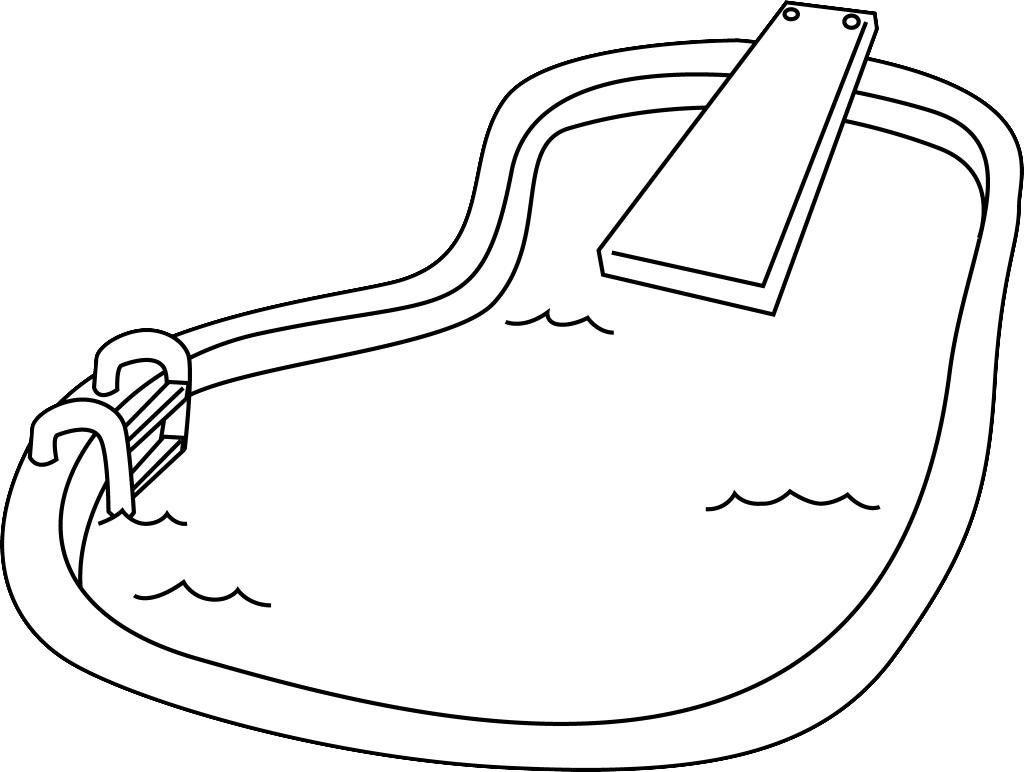
\includegraphics[width=0.4\textwidth]{figs/frontpage/smartpool.png}
\end{minipage}

\vspace{\fill}
\begin{minipage}[l]{\textwidth}
\begin{tabu} to \textwidth{lX[l]}
\textbf{Dato}           &\today\\
\textbf{Vejleder}		&Vejleder navn\\
\end{tabu}
\end{minipage}

\vspace{10pt}
\begin{minipage}[l]{\textwidth}
\tabulinesep=25pt
\begin{tabu} to \textwidth{X[l]X[l]X[l]}
 \makebox[\linewidth]{\hrulefill}\newline Joachim Dam Andersen     \newline 201370248/IKT  
&\makebox[\linewidth]{\hrulefill}\newline Lasse Priebe             \newline 201370248/IKT 
&\makebox[\linewidth]{\hrulefill}\newline Emil Nyborg              \newline 201370248/IKT\\
 \makebox[\linewidth]{\hrulefill}\newline Bjørn Nørgaard Sørensen  \newline 201370248/IKT  
&\makebox[\linewidth]{\hrulefill}\newline Alex Justesen Karlsen    \newline 201370248/IKT 
&\makebox[\linewidth]{\hrulefill}\newline Joachim Händel Noer Wind \newline 201370248/IKT
\end{tabu}
\end{minipage}\clearpage

%% Abstract
% Initial setup
\markboth{RESUMÉ/ABSTRACT}{RESUMÉ/ABSTRACT}
\abstractintoc
\abstractcol
\setlength{\abstitleskip}{-18pt}

% Abstract
\begin{abstract}
Rapporten omhandler et 3. semesterprojekt fra Ingeniørhøjskolen Aarhus Universitet udarbejdet med henblik på at producere et system, som kan fungere som dosering- og sorteringsanlæg til tabletter. Systemet er tiltænkt brug i ældreplejen, som en måde hvorpå fejlmedicinering kan undgås, og tabletsortering kan klares automatisk. Ydermere vil systemet kunne gøre personale og pårørende opmærksomme på, at brugeren ikke har afhentet sine tabletter, indenfor et givet tidsrum. Dette skal formidles ved hjælp af en Android applikation. Systemet og serveren samarbejder om at kontrollerer, hvad der dispenseres til den specifikke bruger og hvornår. Denne kommunikation er ikke fuldt ud implementeret endnu. Systemet var oprindeligt tiltænkt brug i private hjem, men undervejs i processen er idéen ændret idet at fokus flyttes fra private hjem til brug i plejesektoren. 
Produktet kan på nuværende tidspunkt dosere et bestemt antal tabletter af én enkelt type. Systemet har på nuværende tidspunkt allerede implementeret muligheden for at udvide med ekstra dispenserer, og er derfor velegnet til videreudvikling. 
Til systemet er der implementeret en fungerende brugergrænseflade, som er testet med en brugervenlighedsundersøgelse, der ved adspørgelse af 15 studerende har påpeget adskillige muligheder for forbedring.
Under systemudviklingen er den største arbejdsindsats lagt i undersøgelse af teknologier og mulige løsningsforslag.
\end{abstract}

\begin{abstracten}
The report covers a third semesterproject from the Aarhus University School of Engineering. The goal is to produce a system that can function as a dispensing and sorting machine for pills. The system is intended for use in eldercare, as a way of preventing medication errors and a way of sorting pills automaticly. Furthermore, the system will be able to notify staff and relatives if the elder has not picked up their pills, within a given timeperiod. The staff and relatives will be notified via an Android application. The system and a server operate together in order to control what is dispensed to whom and when. Though this communication is not fully implemented yet. The system was originally intended for use in private homes, but during the process, the idea evolved so that the focus was changed from home use to the healthcare sector.
The product can at this time dispense a certain number of pills which will have to be of a single type. The option of adding extra dispensers is already implemented, and is therefore suitable for further development.
The system also has a functioning interface implemented, which has been tested with a user-experience study in which 15 students participated. With the feedback made several things clear, and several of these are suitable for further work.
During the system development the largest effort was put into the study of technologies and potential solutions for the problem chosen.
\end{abstracten}\clearpage

%% Forord
\pagestyle{asereport}
\chapter{Forord}

% Forordet benyttes til at informere kort om visse ydre omstændigheder for projektet, såsom projekttype og hvor projektet er gennemført, historisk baggrund (andre arbejder, som har givet anledning til det aktuelle projekt) og hvor inspirationen og ideen er kommet fra, m.v.

Dette dokument er sammensat for at dokumentere arbejdet på 4. semesterprojektet for retningen IKT på ingeniørhøjskolen Århus.

Der vil i denne rapport være referencer til bilag og dokumentation, som det ikke ville være hensigtsmæssigt at medtage. Samtlige bilag m.m. vil være at finde på den vedlagt CD-rom. 

Source kode til projektet kan findes på CD'en. Link til vores github repo følger her: \newline \url{https://github.com/BjornNorgaard/DuckMaster3001}

\vspace{5mm}

\large{\textit{En stor tak til}}

\begin{displayquote}
    Lars Mortensen for god og brugbar vejledning.
\end{displayquote}

\begin{displayquote}
    Stjerne Apoteket for at lade gruppen komme på besøg og se deres sorteringsmaskine.
\end{displayquote}

\begin{displayquote}
    Sofie Fredslund for at lade os interviewe hende til projektet.
\end{displayquote}

\begin{displayquote}
   Underviserne på ASE, for hjælp og vejledning.
\end{displayquote}

\clearpage

%% ToC
\tableofcontents\clearpage

\mainmatter

%% Todo oversigt - SKAL UDKOMMENTERES FØR AFLEVERING
\listoftodos[Liste over gøremål]

%% Indledning
\chapter{Indledning}

Hello \cite{fysikbog} og sådan kan det jo gå.\clearpage

%% Projektformulering
\documentclass[a4paper,11pt,oneside]{memoir}
\input{utils/packages}
\input{utils/layout}
\input{utils/listings}
\input{utils/ordliste}

%% Forside variabler
\newcommand{\Kursus}{I4PRJ4 F16}
\newcommand{\Projektnavn}{SmartPool 2.0}
\newcommand{\Gruppe}{Gruppe 3}
\newcommand{\Projektdokument}{Projektrapport}

%% Litteratur
\nocite{*}
%\bibliographystyle{harvard}
\bibliography{utils/litteratur}

\begin{document}
\frontmatter

\input{utils/frontpage}\clearpage

%% Abstract
\input{docs/frontmatter/abstract}\clearpage

%% Forord
\pagestyle{asereport}
\input{docs/frontmatter/forord}\clearpage

%% ToC
\tableofcontents\clearpage

\mainmatter

%% Todo oversigt - SKAL UDKOMMENTERES FØR AFLEVERING
\listoftodos[Liste over gøremål]

%% Indledning
\input{docs/frontmatter/indledning}\clearpage

%% Projektformulering
\input{docs/projektformulering/main}\clearpage

%% Kravspecifikation
\input{docs/kravspecifikation/main}\clearpage

%% Systemarkitektur
\input{docs/systemarkitektur/main}\clearpage

%% Processbeskrivelse
\input{docs/processbeskrivelse/main}\clearpage

%% Design
\input{docs/design/main}\clearpage

%% Implementering
\input{docs/implementering/main}\clearpage

%% Integration
\input{docs/integration/main}\clearpage

%% Accepttest
\input{docs/accepttest/main}\clearpage

%% Appendix
\input{docs/appendix/main}\clearpage

\backmatter
%% Glossary
\setglossarystyle{list}
\printnoidxglossary[title=Ordliste]

% Bibliography
\clearpage
\printbibliography[title={Litteratur}]
\end{document}\clearpage

%% Kravspecifikation
\documentclass[a4paper,11pt,oneside]{memoir}
\input{utils/packages}
\input{utils/layout}
\input{utils/listings}
\input{utils/ordliste}

%% Forside variabler
\newcommand{\Kursus}{I4PRJ4 F16}
\newcommand{\Projektnavn}{SmartPool 2.0}
\newcommand{\Gruppe}{Gruppe 3}
\newcommand{\Projektdokument}{Projektrapport}

%% Litteratur
\nocite{*}
%\bibliographystyle{harvard}
\bibliography{utils/litteratur}

\begin{document}
\frontmatter

\input{utils/frontpage}\clearpage

%% Abstract
\input{docs/frontmatter/abstract}\clearpage

%% Forord
\pagestyle{asereport}
\input{docs/frontmatter/forord}\clearpage

%% ToC
\tableofcontents\clearpage

\mainmatter

%% Todo oversigt - SKAL UDKOMMENTERES FØR AFLEVERING
\listoftodos[Liste over gøremål]

%% Indledning
\input{docs/frontmatter/indledning}\clearpage

%% Projektformulering
\input{docs/projektformulering/main}\clearpage

%% Kravspecifikation
\input{docs/kravspecifikation/main}\clearpage

%% Systemarkitektur
\input{docs/systemarkitektur/main}\clearpage

%% Processbeskrivelse
\input{docs/processbeskrivelse/main}\clearpage

%% Design
\input{docs/design/main}\clearpage

%% Implementering
\input{docs/implementering/main}\clearpage

%% Integration
\input{docs/integration/main}\clearpage

%% Accepttest
\input{docs/accepttest/main}\clearpage

%% Appendix
\input{docs/appendix/main}\clearpage

\backmatter
%% Glossary
\setglossarystyle{list}
\printnoidxglossary[title=Ordliste]

% Bibliography
\clearpage
\printbibliography[title={Litteratur}]
\end{document}\clearpage

%% Systemarkitektur
\documentclass[a4paper,11pt,oneside]{memoir}
\input{utils/packages}
\input{utils/layout}
\input{utils/listings}
\input{utils/ordliste}

%% Forside variabler
\newcommand{\Kursus}{I4PRJ4 F16}
\newcommand{\Projektnavn}{SmartPool 2.0}
\newcommand{\Gruppe}{Gruppe 3}
\newcommand{\Projektdokument}{Projektrapport}

%% Litteratur
\nocite{*}
%\bibliographystyle{harvard}
\bibliography{utils/litteratur}

\begin{document}
\frontmatter

\input{utils/frontpage}\clearpage

%% Abstract
\input{docs/frontmatter/abstract}\clearpage

%% Forord
\pagestyle{asereport}
\input{docs/frontmatter/forord}\clearpage

%% ToC
\tableofcontents\clearpage

\mainmatter

%% Todo oversigt - SKAL UDKOMMENTERES FØR AFLEVERING
\listoftodos[Liste over gøremål]

%% Indledning
\input{docs/frontmatter/indledning}\clearpage

%% Projektformulering
\input{docs/projektformulering/main}\clearpage

%% Kravspecifikation
\input{docs/kravspecifikation/main}\clearpage

%% Systemarkitektur
\input{docs/systemarkitektur/main}\clearpage

%% Processbeskrivelse
\input{docs/processbeskrivelse/main}\clearpage

%% Design
\input{docs/design/main}\clearpage

%% Implementering
\input{docs/implementering/main}\clearpage

%% Integration
\input{docs/integration/main}\clearpage

%% Accepttest
\input{docs/accepttest/main}\clearpage

%% Appendix
\input{docs/appendix/main}\clearpage

\backmatter
%% Glossary
\setglossarystyle{list}
\printnoidxglossary[title=Ordliste]

% Bibliography
\clearpage
\printbibliography[title={Litteratur}]
\end{document}\clearpage

%% Processbeskrivelse
\documentclass[a4paper,11pt,oneside]{memoir}
\input{utils/packages}
\input{utils/layout}
\input{utils/listings}
\input{utils/ordliste}

%% Forside variabler
\newcommand{\Kursus}{I4PRJ4 F16}
\newcommand{\Projektnavn}{SmartPool 2.0}
\newcommand{\Gruppe}{Gruppe 3}
\newcommand{\Projektdokument}{Projektrapport}

%% Litteratur
\nocite{*}
%\bibliographystyle{harvard}
\bibliography{utils/litteratur}

\begin{document}
\frontmatter

\input{utils/frontpage}\clearpage

%% Abstract
\input{docs/frontmatter/abstract}\clearpage

%% Forord
\pagestyle{asereport}
\input{docs/frontmatter/forord}\clearpage

%% ToC
\tableofcontents\clearpage

\mainmatter

%% Todo oversigt - SKAL UDKOMMENTERES FØR AFLEVERING
\listoftodos[Liste over gøremål]

%% Indledning
\input{docs/frontmatter/indledning}\clearpage

%% Projektformulering
\input{docs/projektformulering/main}\clearpage

%% Kravspecifikation
\input{docs/kravspecifikation/main}\clearpage

%% Systemarkitektur
\input{docs/systemarkitektur/main}\clearpage

%% Processbeskrivelse
\input{docs/processbeskrivelse/main}\clearpage

%% Design
\input{docs/design/main}\clearpage

%% Implementering
\input{docs/implementering/main}\clearpage

%% Integration
\input{docs/integration/main}\clearpage

%% Accepttest
\input{docs/accepttest/main}\clearpage

%% Appendix
\input{docs/appendix/main}\clearpage

\backmatter
%% Glossary
\setglossarystyle{list}
\printnoidxglossary[title=Ordliste]

% Bibliography
\clearpage
\printbibliography[title={Litteratur}]
\end{document}\clearpage

%% Design
\documentclass[a4paper,11pt,oneside]{memoir}
\input{utils/packages}
\input{utils/layout}
\input{utils/listings}
\input{utils/ordliste}

%% Forside variabler
\newcommand{\Kursus}{I4PRJ4 F16}
\newcommand{\Projektnavn}{SmartPool 2.0}
\newcommand{\Gruppe}{Gruppe 3}
\newcommand{\Projektdokument}{Projektrapport}

%% Litteratur
\nocite{*}
%\bibliographystyle{harvard}
\bibliography{utils/litteratur}

\begin{document}
\frontmatter

\input{utils/frontpage}\clearpage

%% Abstract
\input{docs/frontmatter/abstract}\clearpage

%% Forord
\pagestyle{asereport}
\input{docs/frontmatter/forord}\clearpage

%% ToC
\tableofcontents\clearpage

\mainmatter

%% Todo oversigt - SKAL UDKOMMENTERES FØR AFLEVERING
\listoftodos[Liste over gøremål]

%% Indledning
\input{docs/frontmatter/indledning}\clearpage

%% Projektformulering
\input{docs/projektformulering/main}\clearpage

%% Kravspecifikation
\input{docs/kravspecifikation/main}\clearpage

%% Systemarkitektur
\input{docs/systemarkitektur/main}\clearpage

%% Processbeskrivelse
\input{docs/processbeskrivelse/main}\clearpage

%% Design
\input{docs/design/main}\clearpage

%% Implementering
\input{docs/implementering/main}\clearpage

%% Integration
\input{docs/integration/main}\clearpage

%% Accepttest
\input{docs/accepttest/main}\clearpage

%% Appendix
\input{docs/appendix/main}\clearpage

\backmatter
%% Glossary
\setglossarystyle{list}
\printnoidxglossary[title=Ordliste]

% Bibliography
\clearpage
\printbibliography[title={Litteratur}]
\end{document}\clearpage

%% Implementering
\documentclass[a4paper,11pt,oneside]{memoir}
\input{utils/packages}
\input{utils/layout}
\input{utils/listings}
\input{utils/ordliste}

%% Forside variabler
\newcommand{\Kursus}{I4PRJ4 F16}
\newcommand{\Projektnavn}{SmartPool 2.0}
\newcommand{\Gruppe}{Gruppe 3}
\newcommand{\Projektdokument}{Projektrapport}

%% Litteratur
\nocite{*}
%\bibliographystyle{harvard}
\bibliography{utils/litteratur}

\begin{document}
\frontmatter

\input{utils/frontpage}\clearpage

%% Abstract
\input{docs/frontmatter/abstract}\clearpage

%% Forord
\pagestyle{asereport}
\input{docs/frontmatter/forord}\clearpage

%% ToC
\tableofcontents\clearpage

\mainmatter

%% Todo oversigt - SKAL UDKOMMENTERES FØR AFLEVERING
\listoftodos[Liste over gøremål]

%% Indledning
\input{docs/frontmatter/indledning}\clearpage

%% Projektformulering
\input{docs/projektformulering/main}\clearpage

%% Kravspecifikation
\input{docs/kravspecifikation/main}\clearpage

%% Systemarkitektur
\input{docs/systemarkitektur/main}\clearpage

%% Processbeskrivelse
\input{docs/processbeskrivelse/main}\clearpage

%% Design
\input{docs/design/main}\clearpage

%% Implementering
\input{docs/implementering/main}\clearpage

%% Integration
\input{docs/integration/main}\clearpage

%% Accepttest
\input{docs/accepttest/main}\clearpage

%% Appendix
\input{docs/appendix/main}\clearpage

\backmatter
%% Glossary
\setglossarystyle{list}
\printnoidxglossary[title=Ordliste]

% Bibliography
\clearpage
\printbibliography[title={Litteratur}]
\end{document}\clearpage

%% Integration
\documentclass[a4paper,11pt,oneside]{memoir}
\input{utils/packages}
\input{utils/layout}
\input{utils/listings}
\input{utils/ordliste}

%% Forside variabler
\newcommand{\Kursus}{I4PRJ4 F16}
\newcommand{\Projektnavn}{SmartPool 2.0}
\newcommand{\Gruppe}{Gruppe 3}
\newcommand{\Projektdokument}{Projektrapport}

%% Litteratur
\nocite{*}
%\bibliographystyle{harvard}
\bibliography{utils/litteratur}

\begin{document}
\frontmatter

\input{utils/frontpage}\clearpage

%% Abstract
\input{docs/frontmatter/abstract}\clearpage

%% Forord
\pagestyle{asereport}
\input{docs/frontmatter/forord}\clearpage

%% ToC
\tableofcontents\clearpage

\mainmatter

%% Todo oversigt - SKAL UDKOMMENTERES FØR AFLEVERING
\listoftodos[Liste over gøremål]

%% Indledning
\input{docs/frontmatter/indledning}\clearpage

%% Projektformulering
\input{docs/projektformulering/main}\clearpage

%% Kravspecifikation
\input{docs/kravspecifikation/main}\clearpage

%% Systemarkitektur
\input{docs/systemarkitektur/main}\clearpage

%% Processbeskrivelse
\input{docs/processbeskrivelse/main}\clearpage

%% Design
\input{docs/design/main}\clearpage

%% Implementering
\input{docs/implementering/main}\clearpage

%% Integration
\input{docs/integration/main}\clearpage

%% Accepttest
\input{docs/accepttest/main}\clearpage

%% Appendix
\input{docs/appendix/main}\clearpage

\backmatter
%% Glossary
\setglossarystyle{list}
\printnoidxglossary[title=Ordliste]

% Bibliography
\clearpage
\printbibliography[title={Litteratur}]
\end{document}\clearpage

%% Accepttest
\documentclass[a4paper,11pt,oneside]{memoir}
\input{utils/packages}
\input{utils/layout}
\input{utils/listings}
\input{utils/ordliste}

%% Forside variabler
\newcommand{\Kursus}{I4PRJ4 F16}
\newcommand{\Projektnavn}{SmartPool 2.0}
\newcommand{\Gruppe}{Gruppe 3}
\newcommand{\Projektdokument}{Projektrapport}

%% Litteratur
\nocite{*}
%\bibliographystyle{harvard}
\bibliography{utils/litteratur}

\begin{document}
\frontmatter

\input{utils/frontpage}\clearpage

%% Abstract
\input{docs/frontmatter/abstract}\clearpage

%% Forord
\pagestyle{asereport}
\input{docs/frontmatter/forord}\clearpage

%% ToC
\tableofcontents\clearpage

\mainmatter

%% Todo oversigt - SKAL UDKOMMENTERES FØR AFLEVERING
\listoftodos[Liste over gøremål]

%% Indledning
\input{docs/frontmatter/indledning}\clearpage

%% Projektformulering
\input{docs/projektformulering/main}\clearpage

%% Kravspecifikation
\input{docs/kravspecifikation/main}\clearpage

%% Systemarkitektur
\input{docs/systemarkitektur/main}\clearpage

%% Processbeskrivelse
\input{docs/processbeskrivelse/main}\clearpage

%% Design
\input{docs/design/main}\clearpage

%% Implementering
\input{docs/implementering/main}\clearpage

%% Integration
\input{docs/integration/main}\clearpage

%% Accepttest
\input{docs/accepttest/main}\clearpage

%% Appendix
\input{docs/appendix/main}\clearpage

\backmatter
%% Glossary
\setglossarystyle{list}
\printnoidxglossary[title=Ordliste]

% Bibliography
\clearpage
\printbibliography[title={Litteratur}]
\end{document}\clearpage

%% Appendix
\documentclass[a4paper,11pt,oneside]{memoir}
\input{utils/packages}
\input{utils/layout}
\input{utils/listings}
\input{utils/ordliste}

%% Forside variabler
\newcommand{\Kursus}{I4PRJ4 F16}
\newcommand{\Projektnavn}{SmartPool 2.0}
\newcommand{\Gruppe}{Gruppe 3}
\newcommand{\Projektdokument}{Projektrapport}

%% Litteratur
\nocite{*}
%\bibliographystyle{harvard}
\bibliography{utils/litteratur}

\begin{document}
\frontmatter

\input{utils/frontpage}\clearpage

%% Abstract
\input{docs/frontmatter/abstract}\clearpage

%% Forord
\pagestyle{asereport}
\input{docs/frontmatter/forord}\clearpage

%% ToC
\tableofcontents\clearpage

\mainmatter

%% Todo oversigt - SKAL UDKOMMENTERES FØR AFLEVERING
\listoftodos[Liste over gøremål]

%% Indledning
\input{docs/frontmatter/indledning}\clearpage

%% Projektformulering
\input{docs/projektformulering/main}\clearpage

%% Kravspecifikation
\input{docs/kravspecifikation/main}\clearpage

%% Systemarkitektur
\input{docs/systemarkitektur/main}\clearpage

%% Processbeskrivelse
\input{docs/processbeskrivelse/main}\clearpage

%% Design
\input{docs/design/main}\clearpage

%% Implementering
\input{docs/implementering/main}\clearpage

%% Integration
\input{docs/integration/main}\clearpage

%% Accepttest
\input{docs/accepttest/main}\clearpage

%% Appendix
\input{docs/appendix/main}\clearpage

\backmatter
%% Glossary
\setglossarystyle{list}
\printnoidxglossary[title=Ordliste]

% Bibliography
\clearpage
\printbibliography[title={Litteratur}]
\end{document}\clearpage

\backmatter
%% Glossary
\setglossarystyle{list}
\printnoidxglossary[title=Ordliste]

% Bibliography
\clearpage
\printbibliography[title={Litteratur}]
\end{document}\clearpage

%% Design
\documentclass[a4paper,11pt,oneside]{memoir}
%!TEX root = main.tex
% Encoding
%\usepackage[utf8]{inputenc} % pdfLatex
\usepackage[T1]{fontenc}
\usepackage[danish]{babel}
\renewcommand{\danishhyphenmins}{22}
\usepackage[utf8]{inputenc} % æ ø å

% Date
\usepackage[ddmmyyyy]{datetime}
\renewcommand{\dateseparator}{.}

% Fonts
\usepackage{fourier}
\usepackage[scaled=0.8]{beramono}

% Math
\usepackage{amsmath,amssymb}
\usepackage{bm}
\usepackage{amsthm}
\usepackage{mathtools}

% Graphics
\usepackage[usenames,dvipsnames,table]{xcolor}
\usepackage{graphicx}
\usepackage{float}
%\usepackage[section]{placeins}
\usepackage{tikz}
\usepackage[pages=some]{background}
\usepackage{wrapfig}

% Listings & Tables
\usepackage{listings}
%\usepackage{pythontex}
\usepackage{enumitem}
\usepackage{tabu}
\usepackage{longtable}
\usepackage{multirow}
\usepackage{makecell}


% References & Quotes
%\usepackage[danish]{varioref}				% Muliggoer bl.a. krydshenvisninger med sidetal (\vref)
%\usepackage{nat}							% Udvidelse med naturvidenskabelige citationsmodeller
\usepackage[danish=guillemets]{csquotes}
\usepackage[hidelinks]{hyperref}
\hypersetup{
    pdfstartview={FitH},
    pdftitle={Smart Pool 2.0},
    pdfsubject={Projektrapport},
    pdfauthor={I4PRJ4GRP3}
}
\usepackage[all]{hypcap}

% Etc
\usepackage[
	%backend=biber,
	backend=bibtex,
	style=ieee,
	natbib=true,
	backref=false,
	backrefstyle=all+,
	hyperref=true
]{biblatex}
\usepackage{pdflscape}
\usepackage[nomain,toc,xindy,acronym,nonumberlist,noredefwarn]{glossaries}
\usepackage[xindy]{imakeidx}
\usepackage{float}
\makeindex

% Dummy
\usepackage{lipsum}
%!TEX root = main.tex
% Page setup
\setulmarginsandblock{35mm}{25mm}{*}
\setlrmarginsandblock{20mm}{20mm}{*}
\setheadfoot{4\onelineskip}{2\onelineskip}
\setheaderspaces{*}{5mm}{*}
\checkandfixthelayout

% Pagestyle
\makepagestyle{asereport}
	\makeevenhead{asereport}{}{}{}
	\makeoddhead{asereport}{
\includegraphics{figs/frontpage/aseaulogo.pdf}}{}{\small\rightmark{} | \textbf{\thepage{}\vspace{7pt}}}
	\makeevenfoot{asereport}{}{}{}
	\makeoddfoot{asereport}{}{}{}

\makepsmarks{asereport}{
	\createmark{chapter}{both}{shownumber}{}{. \ }
	\createmark{section}{both}{shownumber}{}{. \ }
	\createmark{subsection}{both}{shownumber}{}{. \ }
	\createplainmark{toc}{both}{\contentsname}
	\createplainmark{lof}{both}{\listfigurename}
	\createplainmark{lot}{both}{\listtablename}
	\createplainmark{bib}{both}{\bibname}
	\createplainmark{index}{both}{\indexname}
	\createplainmark{glossary}{both}{\glossaryname}
}

\aliaspagestyle{part}{asereport}
\aliaspagestyle{chapter}{asereport}
\chapterstyle{tandh}

% Modification to certain spacing
\setlength{\parskip}{8pt}
\setlength{\parindent}{0pt}
\setlength{\abovecaptionskip}{7pt}
\setlength{\belowcaptionskip}{-10pt}
\OnehalfSpacing

% Tabu
%\taburowcolors[1]2{white .. light-gray}
\tabulinesep=4pt

% Itemize/enumerate
\setlist{
    before=\vspace{-3pt}, 
    after=\vspace{-3pt},
    itemsep=0pt,
    leftmargin=25pt,
    labelsep=10pt,
    topsep=0pt,
}

% Kommandoer til UC - fixer spacing
% Aktører
\newcommand{\fua}[1]{
	\begin{minipage}[t]{\linewidth}
		\setlist{
		    leftmargin=22pt,
		    itemsep=0pt,
		    topsep=0pt,
		    parsep=3pt
		}
	\begin{itemize}[before={\vspace{-6pt}}, after={\vspace{6pt}}]
	#1
	\end{itemize}
	\end{minipage}
}

% Hovedforløb
\newcommand{\fu}[1]{
\begin{minipage}[t]{\linewidth}
\setlist{
    leftmargin=22pt,
    itemsep=0pt,
    topsep=0pt,
    parsep=3pt
}
\raggedright
\begin{enumerate}[before={\vspace{-5pt}},after={\vspace{6pt}}]
#1
\end{enumerate}
\end{minipage}}

% Extensions
\newcommand{\fuex}[2]{
\begin{minipage}[t]{\linewidth}
\vspace{-6pt}
\raggedright
\textit{#1}
\begin{enumerate}[leftmargin=22pt,itemsep=0pt,parsep=3pt,before={\vspace{-8pt}}, after={\vspace{20pt}},topsep=8pt]
#2
\end{enumerate}
\end{minipage}
}

% Extensions - Sidste entry
\newcommand{\fuexl}[2]{
\begin{minipage}[t]{\linewidth}
\vspace{-6pt}
\raggedright
\textit{#1}
\begin{enumerate}[leftmargin=22pt,itemsep=0pt,parsep=3pt,before={\vspace{-8pt}}, after={\vspace{3pt}},topsep=8pt]
#2
\end{enumerate}
\end{minipage}}

% Versionshistorik
\newcommand{\verhistitem}[2]{
\begin{minipage}[t]{\linewidth}
\vspace{-6pt}
\raggedright
#1
\begin{itemize}[leftmargin=22pt,itemsep=0pt,parsep=0pt,before={\vspace{-10pt}},after={\vspace{3pt}},topsep=8pt]
#2
\end{itemize}
\end{minipage}}

\newcommand{\tverb}[1]{{\texttt{#1}}}

\newcommand{\cond}[1]{
\begin{itemize}[label=,noitemsep,topsep=0pt,after={\vspace*{-\baselineskip}}]
#1
\end{itemize}}

% Etc
\definecolor{light-gray}{gray}{0.8}
\definecolor{pantone}{RGB}{0,61,133}

\setfloatlocations{figure}{H}
\setfloatlocations{table}{H}

\numberwithin{equation}{chapter}
\numberwithin{figure}{chapter}
\setcounter{secnumdepth}{3}
\setcounter{tocdepth}{2}
\maxsecnumdepth{subsection}

\renewcommand*{\cftdotsep}{1}
\setpnumwidth{2em}
\setrmarg{2em}

\setverbatimfont{\ttfamily}

%\renewcommand\cftchaptername {\chaptername~}
%\renewcommand\cftappendixname {\appendixname~}
\addto\captionsdanish{
    \renewcommand\contentsname{Indholdsfortegnelse}
    \renewcommand\appendixname{Appendiks}
}
\renewcommand\appendixpagename{Appendiks}
\renewcommand\appendixtocname{Appendiks}
\newsubfloat{figure}

% Abstract
\newenvironment{abstracten}
{\renewcommand{\abstractname}{Abstract}\abstract}
{\endabstract}
\renewcommand{\abstractnamefont}{\normalfont\Large\bfseries}
%!TEX root = main.tex
% Listings
\AtBeginDocument{%
  \counterwithin*{lstlisting}{section}
  \counterwithin*{lstlisting}{subsection}
  \counterwithin*{lstlisting}{subsubsection}
  \renewcommand{\thelstlisting}{%
    \ifnum\value{subsection}=0
      \thesection.\arabic{lstlisting}%
    \else
      \ifnum\value{subsubsection}=0
        \thesubsection.\arabic{lstlisting}%
      \else
        \thesubsubsection.\arabic{lstlisting}%
      \fi
    \fi
  }
}

% Loading languages
\lstloadlanguages{C, C++}

% Listing setup
\lstdefinestyle{all}{
    basicstyle    = \ttfamily\SingleSpacing\scriptsize,
    numbers       = left, 
    numberstyle   = \ttfamily\tiny,
    breaklines    = true,
    commentstyle=\color{green},
    %backgroundcolor = \color{red},
    numbersep     = 20pt,
    xleftmargin   = \parindent,
    captionpos    = b,
    keywordstyle  = [1]\color{Blue}\bfseries,
    commentstyle  = \itshape\color{Green},
    tabsize       = 3
}

\lstset{
    style = all
} 
%!TEX root = main.tex
\makenoidxglossaries
\newglossaryentry{gui}{
    name={GUI}, 
    description={Graphical User Interface er en brugergrænseflade. Brugerens måde at tilgå systemet på}}

\newglossaryentry{psoc}{
    name={PSoC}, 
    description={PSoC (Programmable System-on-Chip) er et microcontroller system produceret af Cypress Semiconductor}}

\newglossaryentry{moscow}{
    name={MoSCoW}, 
    description={MoSCoW er en metode til at prioritere krav til ens system}}

\newglossaryentry{furps}{
    name={FURPS}, 
    description={FURPS er en metode til kategorisering af systemets ikke-funktionelle krav}}

\newglossaryentry{BDD}{
    name={BDD}, 
    description={BDD (Block Definition Diagram) er et diagram, som beskriver et system ved at opdele det op i mindre blokke}}

\newglossaryentry{IBD}{
    name={IBD}, 
    description={IBD (Internal Block Diagram) er et diagram, som viser forbindelserne mellem blokkene, som kan findes i et BDD}}

\newglossaryentry{pilleskuffe}{
    name={Pilleskuffe},
    description={Skuffen under dispenseren, hvor i den nederste pille ligger i. Skuffen tømmes ved at elektromagneten trækker skuffen til sig.}}

\newglossaryentry{pilledispenser}{
    name={Pilledispenser},
    description={Det rør som pillerne bliver opbevaret i.}}

\newglossaryentry{elektromagneten}{
    name={Elektromagneten},
    description={Elektromagneten er en spole der sendes strøm igennem. Når der er strøm på spolen dannes et magnetfelt. Der vil ofte være tale om det samme hvad enten der står spole eller elektromagnet.}}

%% Forside variabler
\newcommand{\Kursus}{I4PRJ4 F16}
\newcommand{\Projektnavn}{SmartPool 2.0}
\newcommand{\Gruppe}{Gruppe 3}
\newcommand{\Projektdokument}{Projektrapport}

%% Litteratur
\nocite{*}
%\bibliographystyle{harvard}
\bibliography{utils/litteratur}

\begin{document}
\frontmatter

%!TEX root = main.tex
\pagestyle{titlingpage}
\backgroundsetup{
	scale=1,
	angle=0,
	opacity=1,
	contents={
		\begin{tikzpicture}[remember picture,overlay]
		\path [fill=pantone] (-0.5\paperwidth,0.36\paperheight) rectangle (0.5\paperwidth,0.47\paperheight);  
		\path [fill=pantone] (-0.5\paperwidth,-0.47\paperheight) rectangle (0.5\paperwidth,-0.43\paperheight);  
		\end{tikzpicture}}}
\BgThispage
\vspace*{-25mm}
\begin{minipage}[l]{\textwidth}
	
\includegraphics[width=0.75\textwidth]{figs/frontpage/aseaulogohvid.pdf}
\end{minipage}

\vspace{35pt}
\begin{minipage}[l]{\textwidth}
\tabulinesep=10pt
\begin{tabu} to \textwidth{X[l]}
	{\small\MakeUppercase\Kursus}\\
	{\HUGE\bfseries\MakeUppercase\Projektnavn}\\
	{\Large\Gruppe}\\
	{\itshape\Projektdokument}
\end{tabu}
\end{minipage}

\vspace{5pt}
\begin{minipage}[l]{\textwidth}
    \centering
	\vspace*{0cm}\hspace*{8cm}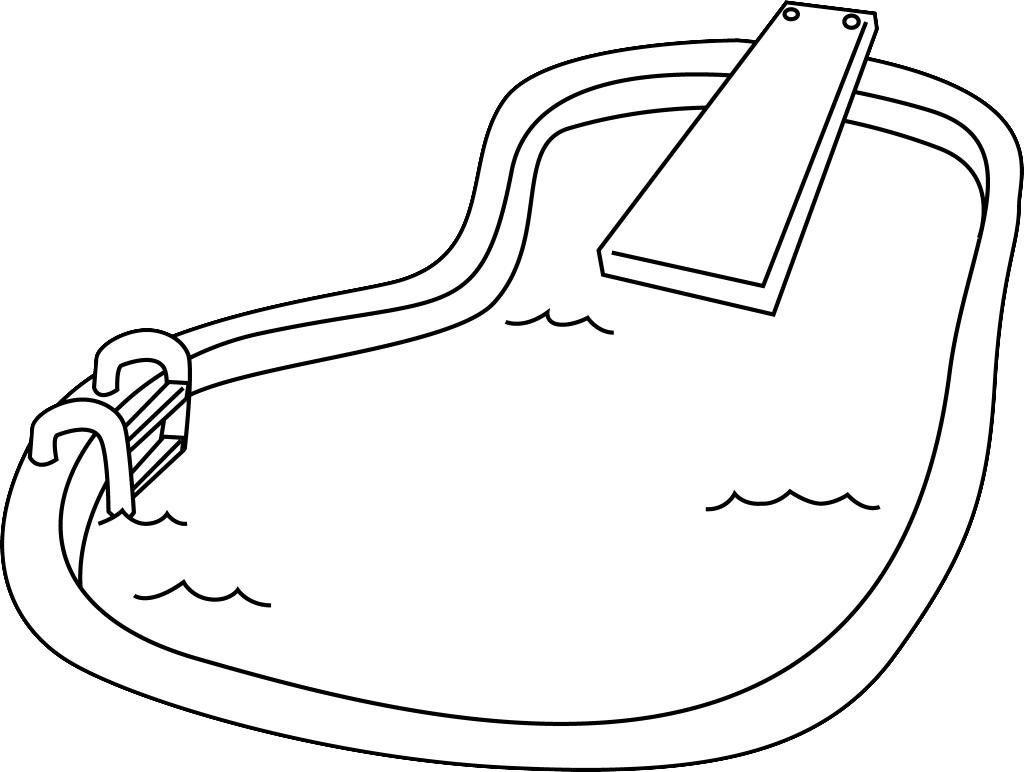
\includegraphics[width=0.4\textwidth]{figs/frontpage/smartpool.png}
\end{minipage}

\vspace{\fill}
\begin{minipage}[l]{\textwidth}
\begin{tabu} to \textwidth{lX[l]}
\textbf{Dato}           &\today\\
\textbf{Vejleder}		&Vejleder navn\\
\end{tabu}
\end{minipage}

\vspace{10pt}
\begin{minipage}[l]{\textwidth}
\tabulinesep=25pt
\begin{tabu} to \textwidth{X[l]X[l]X[l]}
 \makebox[\linewidth]{\hrulefill}\newline Joachim Dam Andersen     \newline 201370248/IKT  
&\makebox[\linewidth]{\hrulefill}\newline Lasse Priebe             \newline 201370248/IKT 
&\makebox[\linewidth]{\hrulefill}\newline Emil Nyborg              \newline 201370248/IKT\\
 \makebox[\linewidth]{\hrulefill}\newline Bjørn Nørgaard Sørensen  \newline 201370248/IKT  
&\makebox[\linewidth]{\hrulefill}\newline Alex Justesen Karlsen    \newline 201370248/IKT 
&\makebox[\linewidth]{\hrulefill}\newline Joachim Händel Noer Wind \newline 201370248/IKT
\end{tabu}
\end{minipage}\clearpage

%% Abstract
% Initial setup
\markboth{RESUMÉ/ABSTRACT}{RESUMÉ/ABSTRACT}
\abstractintoc
\abstractcol
\setlength{\abstitleskip}{-18pt}

% Abstract
\begin{abstract}
Rapporten omhandler et 3. semesterprojekt fra Ingeniørhøjskolen Aarhus Universitet udarbejdet med henblik på at producere et system, som kan fungere som dosering- og sorteringsanlæg til tabletter. Systemet er tiltænkt brug i ældreplejen, som en måde hvorpå fejlmedicinering kan undgås, og tabletsortering kan klares automatisk. Ydermere vil systemet kunne gøre personale og pårørende opmærksomme på, at brugeren ikke har afhentet sine tabletter, indenfor et givet tidsrum. Dette skal formidles ved hjælp af en Android applikation. Systemet og serveren samarbejder om at kontrollerer, hvad der dispenseres til den specifikke bruger og hvornår. Denne kommunikation er ikke fuldt ud implementeret endnu. Systemet var oprindeligt tiltænkt brug i private hjem, men undervejs i processen er idéen ændret idet at fokus flyttes fra private hjem til brug i plejesektoren. 
Produktet kan på nuværende tidspunkt dosere et bestemt antal tabletter af én enkelt type. Systemet har på nuværende tidspunkt allerede implementeret muligheden for at udvide med ekstra dispenserer, og er derfor velegnet til videreudvikling. 
Til systemet er der implementeret en fungerende brugergrænseflade, som er testet med en brugervenlighedsundersøgelse, der ved adspørgelse af 15 studerende har påpeget adskillige muligheder for forbedring.
Under systemudviklingen er den største arbejdsindsats lagt i undersøgelse af teknologier og mulige løsningsforslag.
\end{abstract}

\begin{abstracten}
The report covers a third semesterproject from the Aarhus University School of Engineering. The goal is to produce a system that can function as a dispensing and sorting machine for pills. The system is intended for use in eldercare, as a way of preventing medication errors and a way of sorting pills automaticly. Furthermore, the system will be able to notify staff and relatives if the elder has not picked up their pills, within a given timeperiod. The staff and relatives will be notified via an Android application. The system and a server operate together in order to control what is dispensed to whom and when. Though this communication is not fully implemented yet. The system was originally intended for use in private homes, but during the process, the idea evolved so that the focus was changed from home use to the healthcare sector.
The product can at this time dispense a certain number of pills which will have to be of a single type. The option of adding extra dispensers is already implemented, and is therefore suitable for further development.
The system also has a functioning interface implemented, which has been tested with a user-experience study in which 15 students participated. With the feedback made several things clear, and several of these are suitable for further work.
During the system development the largest effort was put into the study of technologies and potential solutions for the problem chosen.
\end{abstracten}\clearpage

%% Forord
\pagestyle{asereport}
\chapter{Forord}

% Forordet benyttes til at informere kort om visse ydre omstændigheder for projektet, såsom projekttype og hvor projektet er gennemført, historisk baggrund (andre arbejder, som har givet anledning til det aktuelle projekt) og hvor inspirationen og ideen er kommet fra, m.v.

Dette dokument er sammensat for at dokumentere arbejdet på 4. semesterprojektet for retningen IKT på ingeniørhøjskolen Århus.

Der vil i denne rapport være referencer til bilag og dokumentation, som det ikke ville være hensigtsmæssigt at medtage. Samtlige bilag m.m. vil være at finde på den vedlagt CD-rom. 

Source kode til projektet kan findes på CD'en. Link til vores github repo følger her: \newline \url{https://github.com/BjornNorgaard/DuckMaster3001}

\vspace{5mm}

\large{\textit{En stor tak til}}

\begin{displayquote}
    Lars Mortensen for god og brugbar vejledning.
\end{displayquote}

\begin{displayquote}
    Stjerne Apoteket for at lade gruppen komme på besøg og se deres sorteringsmaskine.
\end{displayquote}

\begin{displayquote}
    Sofie Fredslund for at lade os interviewe hende til projektet.
\end{displayquote}

\begin{displayquote}
   Underviserne på ASE, for hjælp og vejledning.
\end{displayquote}

\clearpage

%% ToC
\tableofcontents\clearpage

\mainmatter

%% Todo oversigt - SKAL UDKOMMENTERES FØR AFLEVERING
\listoftodos[Liste over gøremål]

%% Indledning
\chapter{Indledning}

Hello \cite{fysikbog} og sådan kan det jo gå.\clearpage

%% Projektformulering
\documentclass[a4paper,11pt,oneside]{memoir}
\input{utils/packages}
\input{utils/layout}
\input{utils/listings}
\input{utils/ordliste}

%% Forside variabler
\newcommand{\Kursus}{I4PRJ4 F16}
\newcommand{\Projektnavn}{SmartPool 2.0}
\newcommand{\Gruppe}{Gruppe 3}
\newcommand{\Projektdokument}{Projektrapport}

%% Litteratur
\nocite{*}
%\bibliographystyle{harvard}
\bibliography{utils/litteratur}

\begin{document}
\frontmatter

\input{utils/frontpage}\clearpage

%% Abstract
\input{docs/frontmatter/abstract}\clearpage

%% Forord
\pagestyle{asereport}
\input{docs/frontmatter/forord}\clearpage

%% ToC
\tableofcontents\clearpage

\mainmatter

%% Todo oversigt - SKAL UDKOMMENTERES FØR AFLEVERING
\listoftodos[Liste over gøremål]

%% Indledning
\input{docs/frontmatter/indledning}\clearpage

%% Projektformulering
\input{docs/projektformulering/main}\clearpage

%% Kravspecifikation
\input{docs/kravspecifikation/main}\clearpage

%% Systemarkitektur
\input{docs/systemarkitektur/main}\clearpage

%% Processbeskrivelse
\input{docs/processbeskrivelse/main}\clearpage

%% Design
\input{docs/design/main}\clearpage

%% Implementering
\input{docs/implementering/main}\clearpage

%% Integration
\input{docs/integration/main}\clearpage

%% Accepttest
\input{docs/accepttest/main}\clearpage

%% Appendix
\input{docs/appendix/main}\clearpage

\backmatter
%% Glossary
\setglossarystyle{list}
\printnoidxglossary[title=Ordliste]

% Bibliography
\clearpage
\printbibliography[title={Litteratur}]
\end{document}\clearpage

%% Kravspecifikation
\documentclass[a4paper,11pt,oneside]{memoir}
\input{utils/packages}
\input{utils/layout}
\input{utils/listings}
\input{utils/ordliste}

%% Forside variabler
\newcommand{\Kursus}{I4PRJ4 F16}
\newcommand{\Projektnavn}{SmartPool 2.0}
\newcommand{\Gruppe}{Gruppe 3}
\newcommand{\Projektdokument}{Projektrapport}

%% Litteratur
\nocite{*}
%\bibliographystyle{harvard}
\bibliography{utils/litteratur}

\begin{document}
\frontmatter

\input{utils/frontpage}\clearpage

%% Abstract
\input{docs/frontmatter/abstract}\clearpage

%% Forord
\pagestyle{asereport}
\input{docs/frontmatter/forord}\clearpage

%% ToC
\tableofcontents\clearpage

\mainmatter

%% Todo oversigt - SKAL UDKOMMENTERES FØR AFLEVERING
\listoftodos[Liste over gøremål]

%% Indledning
\input{docs/frontmatter/indledning}\clearpage

%% Projektformulering
\input{docs/projektformulering/main}\clearpage

%% Kravspecifikation
\input{docs/kravspecifikation/main}\clearpage

%% Systemarkitektur
\input{docs/systemarkitektur/main}\clearpage

%% Processbeskrivelse
\input{docs/processbeskrivelse/main}\clearpage

%% Design
\input{docs/design/main}\clearpage

%% Implementering
\input{docs/implementering/main}\clearpage

%% Integration
\input{docs/integration/main}\clearpage

%% Accepttest
\input{docs/accepttest/main}\clearpage

%% Appendix
\input{docs/appendix/main}\clearpage

\backmatter
%% Glossary
\setglossarystyle{list}
\printnoidxglossary[title=Ordliste]

% Bibliography
\clearpage
\printbibliography[title={Litteratur}]
\end{document}\clearpage

%% Systemarkitektur
\documentclass[a4paper,11pt,oneside]{memoir}
\input{utils/packages}
\input{utils/layout}
\input{utils/listings}
\input{utils/ordliste}

%% Forside variabler
\newcommand{\Kursus}{I4PRJ4 F16}
\newcommand{\Projektnavn}{SmartPool 2.0}
\newcommand{\Gruppe}{Gruppe 3}
\newcommand{\Projektdokument}{Projektrapport}

%% Litteratur
\nocite{*}
%\bibliographystyle{harvard}
\bibliography{utils/litteratur}

\begin{document}
\frontmatter

\input{utils/frontpage}\clearpage

%% Abstract
\input{docs/frontmatter/abstract}\clearpage

%% Forord
\pagestyle{asereport}
\input{docs/frontmatter/forord}\clearpage

%% ToC
\tableofcontents\clearpage

\mainmatter

%% Todo oversigt - SKAL UDKOMMENTERES FØR AFLEVERING
\listoftodos[Liste over gøremål]

%% Indledning
\input{docs/frontmatter/indledning}\clearpage

%% Projektformulering
\input{docs/projektformulering/main}\clearpage

%% Kravspecifikation
\input{docs/kravspecifikation/main}\clearpage

%% Systemarkitektur
\input{docs/systemarkitektur/main}\clearpage

%% Processbeskrivelse
\input{docs/processbeskrivelse/main}\clearpage

%% Design
\input{docs/design/main}\clearpage

%% Implementering
\input{docs/implementering/main}\clearpage

%% Integration
\input{docs/integration/main}\clearpage

%% Accepttest
\input{docs/accepttest/main}\clearpage

%% Appendix
\input{docs/appendix/main}\clearpage

\backmatter
%% Glossary
\setglossarystyle{list}
\printnoidxglossary[title=Ordliste]

% Bibliography
\clearpage
\printbibliography[title={Litteratur}]
\end{document}\clearpage

%% Processbeskrivelse
\documentclass[a4paper,11pt,oneside]{memoir}
\input{utils/packages}
\input{utils/layout}
\input{utils/listings}
\input{utils/ordliste}

%% Forside variabler
\newcommand{\Kursus}{I4PRJ4 F16}
\newcommand{\Projektnavn}{SmartPool 2.0}
\newcommand{\Gruppe}{Gruppe 3}
\newcommand{\Projektdokument}{Projektrapport}

%% Litteratur
\nocite{*}
%\bibliographystyle{harvard}
\bibliography{utils/litteratur}

\begin{document}
\frontmatter

\input{utils/frontpage}\clearpage

%% Abstract
\input{docs/frontmatter/abstract}\clearpage

%% Forord
\pagestyle{asereport}
\input{docs/frontmatter/forord}\clearpage

%% ToC
\tableofcontents\clearpage

\mainmatter

%% Todo oversigt - SKAL UDKOMMENTERES FØR AFLEVERING
\listoftodos[Liste over gøremål]

%% Indledning
\input{docs/frontmatter/indledning}\clearpage

%% Projektformulering
\input{docs/projektformulering/main}\clearpage

%% Kravspecifikation
\input{docs/kravspecifikation/main}\clearpage

%% Systemarkitektur
\input{docs/systemarkitektur/main}\clearpage

%% Processbeskrivelse
\input{docs/processbeskrivelse/main}\clearpage

%% Design
\input{docs/design/main}\clearpage

%% Implementering
\input{docs/implementering/main}\clearpage

%% Integration
\input{docs/integration/main}\clearpage

%% Accepttest
\input{docs/accepttest/main}\clearpage

%% Appendix
\input{docs/appendix/main}\clearpage

\backmatter
%% Glossary
\setglossarystyle{list}
\printnoidxglossary[title=Ordliste]

% Bibliography
\clearpage
\printbibliography[title={Litteratur}]
\end{document}\clearpage

%% Design
\documentclass[a4paper,11pt,oneside]{memoir}
\input{utils/packages}
\input{utils/layout}
\input{utils/listings}
\input{utils/ordliste}

%% Forside variabler
\newcommand{\Kursus}{I4PRJ4 F16}
\newcommand{\Projektnavn}{SmartPool 2.0}
\newcommand{\Gruppe}{Gruppe 3}
\newcommand{\Projektdokument}{Projektrapport}

%% Litteratur
\nocite{*}
%\bibliographystyle{harvard}
\bibliography{utils/litteratur}

\begin{document}
\frontmatter

\input{utils/frontpage}\clearpage

%% Abstract
\input{docs/frontmatter/abstract}\clearpage

%% Forord
\pagestyle{asereport}
\input{docs/frontmatter/forord}\clearpage

%% ToC
\tableofcontents\clearpage

\mainmatter

%% Todo oversigt - SKAL UDKOMMENTERES FØR AFLEVERING
\listoftodos[Liste over gøremål]

%% Indledning
\input{docs/frontmatter/indledning}\clearpage

%% Projektformulering
\input{docs/projektformulering/main}\clearpage

%% Kravspecifikation
\input{docs/kravspecifikation/main}\clearpage

%% Systemarkitektur
\input{docs/systemarkitektur/main}\clearpage

%% Processbeskrivelse
\input{docs/processbeskrivelse/main}\clearpage

%% Design
\input{docs/design/main}\clearpage

%% Implementering
\input{docs/implementering/main}\clearpage

%% Integration
\input{docs/integration/main}\clearpage

%% Accepttest
\input{docs/accepttest/main}\clearpage

%% Appendix
\input{docs/appendix/main}\clearpage

\backmatter
%% Glossary
\setglossarystyle{list}
\printnoidxglossary[title=Ordliste]

% Bibliography
\clearpage
\printbibliography[title={Litteratur}]
\end{document}\clearpage

%% Implementering
\documentclass[a4paper,11pt,oneside]{memoir}
\input{utils/packages}
\input{utils/layout}
\input{utils/listings}
\input{utils/ordliste}

%% Forside variabler
\newcommand{\Kursus}{I4PRJ4 F16}
\newcommand{\Projektnavn}{SmartPool 2.0}
\newcommand{\Gruppe}{Gruppe 3}
\newcommand{\Projektdokument}{Projektrapport}

%% Litteratur
\nocite{*}
%\bibliographystyle{harvard}
\bibliography{utils/litteratur}

\begin{document}
\frontmatter

\input{utils/frontpage}\clearpage

%% Abstract
\input{docs/frontmatter/abstract}\clearpage

%% Forord
\pagestyle{asereport}
\input{docs/frontmatter/forord}\clearpage

%% ToC
\tableofcontents\clearpage

\mainmatter

%% Todo oversigt - SKAL UDKOMMENTERES FØR AFLEVERING
\listoftodos[Liste over gøremål]

%% Indledning
\input{docs/frontmatter/indledning}\clearpage

%% Projektformulering
\input{docs/projektformulering/main}\clearpage

%% Kravspecifikation
\input{docs/kravspecifikation/main}\clearpage

%% Systemarkitektur
\input{docs/systemarkitektur/main}\clearpage

%% Processbeskrivelse
\input{docs/processbeskrivelse/main}\clearpage

%% Design
\input{docs/design/main}\clearpage

%% Implementering
\input{docs/implementering/main}\clearpage

%% Integration
\input{docs/integration/main}\clearpage

%% Accepttest
\input{docs/accepttest/main}\clearpage

%% Appendix
\input{docs/appendix/main}\clearpage

\backmatter
%% Glossary
\setglossarystyle{list}
\printnoidxglossary[title=Ordliste]

% Bibliography
\clearpage
\printbibliography[title={Litteratur}]
\end{document}\clearpage

%% Integration
\documentclass[a4paper,11pt,oneside]{memoir}
\input{utils/packages}
\input{utils/layout}
\input{utils/listings}
\input{utils/ordliste}

%% Forside variabler
\newcommand{\Kursus}{I4PRJ4 F16}
\newcommand{\Projektnavn}{SmartPool 2.0}
\newcommand{\Gruppe}{Gruppe 3}
\newcommand{\Projektdokument}{Projektrapport}

%% Litteratur
\nocite{*}
%\bibliographystyle{harvard}
\bibliography{utils/litteratur}

\begin{document}
\frontmatter

\input{utils/frontpage}\clearpage

%% Abstract
\input{docs/frontmatter/abstract}\clearpage

%% Forord
\pagestyle{asereport}
\input{docs/frontmatter/forord}\clearpage

%% ToC
\tableofcontents\clearpage

\mainmatter

%% Todo oversigt - SKAL UDKOMMENTERES FØR AFLEVERING
\listoftodos[Liste over gøremål]

%% Indledning
\input{docs/frontmatter/indledning}\clearpage

%% Projektformulering
\input{docs/projektformulering/main}\clearpage

%% Kravspecifikation
\input{docs/kravspecifikation/main}\clearpage

%% Systemarkitektur
\input{docs/systemarkitektur/main}\clearpage

%% Processbeskrivelse
\input{docs/processbeskrivelse/main}\clearpage

%% Design
\input{docs/design/main}\clearpage

%% Implementering
\input{docs/implementering/main}\clearpage

%% Integration
\input{docs/integration/main}\clearpage

%% Accepttest
\input{docs/accepttest/main}\clearpage

%% Appendix
\input{docs/appendix/main}\clearpage

\backmatter
%% Glossary
\setglossarystyle{list}
\printnoidxglossary[title=Ordliste]

% Bibliography
\clearpage
\printbibliography[title={Litteratur}]
\end{document}\clearpage

%% Accepttest
\documentclass[a4paper,11pt,oneside]{memoir}
\input{utils/packages}
\input{utils/layout}
\input{utils/listings}
\input{utils/ordliste}

%% Forside variabler
\newcommand{\Kursus}{I4PRJ4 F16}
\newcommand{\Projektnavn}{SmartPool 2.0}
\newcommand{\Gruppe}{Gruppe 3}
\newcommand{\Projektdokument}{Projektrapport}

%% Litteratur
\nocite{*}
%\bibliographystyle{harvard}
\bibliography{utils/litteratur}

\begin{document}
\frontmatter

\input{utils/frontpage}\clearpage

%% Abstract
\input{docs/frontmatter/abstract}\clearpage

%% Forord
\pagestyle{asereport}
\input{docs/frontmatter/forord}\clearpage

%% ToC
\tableofcontents\clearpage

\mainmatter

%% Todo oversigt - SKAL UDKOMMENTERES FØR AFLEVERING
\listoftodos[Liste over gøremål]

%% Indledning
\input{docs/frontmatter/indledning}\clearpage

%% Projektformulering
\input{docs/projektformulering/main}\clearpage

%% Kravspecifikation
\input{docs/kravspecifikation/main}\clearpage

%% Systemarkitektur
\input{docs/systemarkitektur/main}\clearpage

%% Processbeskrivelse
\input{docs/processbeskrivelse/main}\clearpage

%% Design
\input{docs/design/main}\clearpage

%% Implementering
\input{docs/implementering/main}\clearpage

%% Integration
\input{docs/integration/main}\clearpage

%% Accepttest
\input{docs/accepttest/main}\clearpage

%% Appendix
\input{docs/appendix/main}\clearpage

\backmatter
%% Glossary
\setglossarystyle{list}
\printnoidxglossary[title=Ordliste]

% Bibliography
\clearpage
\printbibliography[title={Litteratur}]
\end{document}\clearpage

%% Appendix
\documentclass[a4paper,11pt,oneside]{memoir}
\input{utils/packages}
\input{utils/layout}
\input{utils/listings}
\input{utils/ordliste}

%% Forside variabler
\newcommand{\Kursus}{I4PRJ4 F16}
\newcommand{\Projektnavn}{SmartPool 2.0}
\newcommand{\Gruppe}{Gruppe 3}
\newcommand{\Projektdokument}{Projektrapport}

%% Litteratur
\nocite{*}
%\bibliographystyle{harvard}
\bibliography{utils/litteratur}

\begin{document}
\frontmatter

\input{utils/frontpage}\clearpage

%% Abstract
\input{docs/frontmatter/abstract}\clearpage

%% Forord
\pagestyle{asereport}
\input{docs/frontmatter/forord}\clearpage

%% ToC
\tableofcontents\clearpage

\mainmatter

%% Todo oversigt - SKAL UDKOMMENTERES FØR AFLEVERING
\listoftodos[Liste over gøremål]

%% Indledning
\input{docs/frontmatter/indledning}\clearpage

%% Projektformulering
\input{docs/projektformulering/main}\clearpage

%% Kravspecifikation
\input{docs/kravspecifikation/main}\clearpage

%% Systemarkitektur
\input{docs/systemarkitektur/main}\clearpage

%% Processbeskrivelse
\input{docs/processbeskrivelse/main}\clearpage

%% Design
\input{docs/design/main}\clearpage

%% Implementering
\input{docs/implementering/main}\clearpage

%% Integration
\input{docs/integration/main}\clearpage

%% Accepttest
\input{docs/accepttest/main}\clearpage

%% Appendix
\input{docs/appendix/main}\clearpage

\backmatter
%% Glossary
\setglossarystyle{list}
\printnoidxglossary[title=Ordliste]

% Bibliography
\clearpage
\printbibliography[title={Litteratur}]
\end{document}\clearpage

\backmatter
%% Glossary
\setglossarystyle{list}
\printnoidxglossary[title=Ordliste]

% Bibliography
\clearpage
\printbibliography[title={Litteratur}]
\end{document}\clearpage

%% Implementering
\documentclass[a4paper,11pt,oneside]{memoir}
%!TEX root = main.tex
% Encoding
%\usepackage[utf8]{inputenc} % pdfLatex
\usepackage[T1]{fontenc}
\usepackage[danish]{babel}
\renewcommand{\danishhyphenmins}{22}
\usepackage[utf8]{inputenc} % æ ø å

% Date
\usepackage[ddmmyyyy]{datetime}
\renewcommand{\dateseparator}{.}

% Fonts
\usepackage{fourier}
\usepackage[scaled=0.8]{beramono}

% Math
\usepackage{amsmath,amssymb}
\usepackage{bm}
\usepackage{amsthm}
\usepackage{mathtools}

% Graphics
\usepackage[usenames,dvipsnames,table]{xcolor}
\usepackage{graphicx}
\usepackage{float}
%\usepackage[section]{placeins}
\usepackage{tikz}
\usepackage[pages=some]{background}
\usepackage{wrapfig}

% Listings & Tables
\usepackage{listings}
%\usepackage{pythontex}
\usepackage{enumitem}
\usepackage{tabu}
\usepackage{longtable}
\usepackage{multirow}
\usepackage{makecell}


% References & Quotes
%\usepackage[danish]{varioref}				% Muliggoer bl.a. krydshenvisninger med sidetal (\vref)
%\usepackage{nat}							% Udvidelse med naturvidenskabelige citationsmodeller
\usepackage[danish=guillemets]{csquotes}
\usepackage[hidelinks]{hyperref}
\hypersetup{
    pdfstartview={FitH},
    pdftitle={Smart Pool 2.0},
    pdfsubject={Projektrapport},
    pdfauthor={I4PRJ4GRP3}
}
\usepackage[all]{hypcap}

% Etc
\usepackage[
	%backend=biber,
	backend=bibtex,
	style=ieee,
	natbib=true,
	backref=false,
	backrefstyle=all+,
	hyperref=true
]{biblatex}
\usepackage{pdflscape}
\usepackage[nomain,toc,xindy,acronym,nonumberlist,noredefwarn]{glossaries}
\usepackage[xindy]{imakeidx}
\usepackage{float}
\makeindex

% Dummy
\usepackage{lipsum}
%!TEX root = main.tex
% Page setup
\setulmarginsandblock{35mm}{25mm}{*}
\setlrmarginsandblock{20mm}{20mm}{*}
\setheadfoot{4\onelineskip}{2\onelineskip}
\setheaderspaces{*}{5mm}{*}
\checkandfixthelayout

% Pagestyle
\makepagestyle{asereport}
	\makeevenhead{asereport}{}{}{}
	\makeoddhead{asereport}{
\includegraphics{figs/frontpage/aseaulogo.pdf}}{}{\small\rightmark{} | \textbf{\thepage{}\vspace{7pt}}}
	\makeevenfoot{asereport}{}{}{}
	\makeoddfoot{asereport}{}{}{}

\makepsmarks{asereport}{
	\createmark{chapter}{both}{shownumber}{}{. \ }
	\createmark{section}{both}{shownumber}{}{. \ }
	\createmark{subsection}{both}{shownumber}{}{. \ }
	\createplainmark{toc}{both}{\contentsname}
	\createplainmark{lof}{both}{\listfigurename}
	\createplainmark{lot}{both}{\listtablename}
	\createplainmark{bib}{both}{\bibname}
	\createplainmark{index}{both}{\indexname}
	\createplainmark{glossary}{both}{\glossaryname}
}

\aliaspagestyle{part}{asereport}
\aliaspagestyle{chapter}{asereport}
\chapterstyle{tandh}

% Modification to certain spacing
\setlength{\parskip}{8pt}
\setlength{\parindent}{0pt}
\setlength{\abovecaptionskip}{7pt}
\setlength{\belowcaptionskip}{-10pt}
\OnehalfSpacing

% Tabu
%\taburowcolors[1]2{white .. light-gray}
\tabulinesep=4pt

% Itemize/enumerate
\setlist{
    before=\vspace{-3pt}, 
    after=\vspace{-3pt},
    itemsep=0pt,
    leftmargin=25pt,
    labelsep=10pt,
    topsep=0pt,
}

% Kommandoer til UC - fixer spacing
% Aktører
\newcommand{\fua}[1]{
	\begin{minipage}[t]{\linewidth}
		\setlist{
		    leftmargin=22pt,
		    itemsep=0pt,
		    topsep=0pt,
		    parsep=3pt
		}
	\begin{itemize}[before={\vspace{-6pt}}, after={\vspace{6pt}}]
	#1
	\end{itemize}
	\end{minipage}
}

% Hovedforløb
\newcommand{\fu}[1]{
\begin{minipage}[t]{\linewidth}
\setlist{
    leftmargin=22pt,
    itemsep=0pt,
    topsep=0pt,
    parsep=3pt
}
\raggedright
\begin{enumerate}[before={\vspace{-5pt}},after={\vspace{6pt}}]
#1
\end{enumerate}
\end{minipage}}

% Extensions
\newcommand{\fuex}[2]{
\begin{minipage}[t]{\linewidth}
\vspace{-6pt}
\raggedright
\textit{#1}
\begin{enumerate}[leftmargin=22pt,itemsep=0pt,parsep=3pt,before={\vspace{-8pt}}, after={\vspace{20pt}},topsep=8pt]
#2
\end{enumerate}
\end{minipage}
}

% Extensions - Sidste entry
\newcommand{\fuexl}[2]{
\begin{minipage}[t]{\linewidth}
\vspace{-6pt}
\raggedright
\textit{#1}
\begin{enumerate}[leftmargin=22pt,itemsep=0pt,parsep=3pt,before={\vspace{-8pt}}, after={\vspace{3pt}},topsep=8pt]
#2
\end{enumerate}
\end{minipage}}

% Versionshistorik
\newcommand{\verhistitem}[2]{
\begin{minipage}[t]{\linewidth}
\vspace{-6pt}
\raggedright
#1
\begin{itemize}[leftmargin=22pt,itemsep=0pt,parsep=0pt,before={\vspace{-10pt}},after={\vspace{3pt}},topsep=8pt]
#2
\end{itemize}
\end{minipage}}

\newcommand{\tverb}[1]{{\texttt{#1}}}

\newcommand{\cond}[1]{
\begin{itemize}[label=,noitemsep,topsep=0pt,after={\vspace*{-\baselineskip}}]
#1
\end{itemize}}

% Etc
\definecolor{light-gray}{gray}{0.8}
\definecolor{pantone}{RGB}{0,61,133}

\setfloatlocations{figure}{H}
\setfloatlocations{table}{H}

\numberwithin{equation}{chapter}
\numberwithin{figure}{chapter}
\setcounter{secnumdepth}{3}
\setcounter{tocdepth}{2}
\maxsecnumdepth{subsection}

\renewcommand*{\cftdotsep}{1}
\setpnumwidth{2em}
\setrmarg{2em}

\setverbatimfont{\ttfamily}

%\renewcommand\cftchaptername {\chaptername~}
%\renewcommand\cftappendixname {\appendixname~}
\addto\captionsdanish{
    \renewcommand\contentsname{Indholdsfortegnelse}
    \renewcommand\appendixname{Appendiks}
}
\renewcommand\appendixpagename{Appendiks}
\renewcommand\appendixtocname{Appendiks}
\newsubfloat{figure}

% Abstract
\newenvironment{abstracten}
{\renewcommand{\abstractname}{Abstract}\abstract}
{\endabstract}
\renewcommand{\abstractnamefont}{\normalfont\Large\bfseries}
%!TEX root = main.tex
% Listings
\AtBeginDocument{%
  \counterwithin*{lstlisting}{section}
  \counterwithin*{lstlisting}{subsection}
  \counterwithin*{lstlisting}{subsubsection}
  \renewcommand{\thelstlisting}{%
    \ifnum\value{subsection}=0
      \thesection.\arabic{lstlisting}%
    \else
      \ifnum\value{subsubsection}=0
        \thesubsection.\arabic{lstlisting}%
      \else
        \thesubsubsection.\arabic{lstlisting}%
      \fi
    \fi
  }
}

% Loading languages
\lstloadlanguages{C, C++}

% Listing setup
\lstdefinestyle{all}{
    basicstyle    = \ttfamily\SingleSpacing\scriptsize,
    numbers       = left, 
    numberstyle   = \ttfamily\tiny,
    breaklines    = true,
    commentstyle=\color{green},
    %backgroundcolor = \color{red},
    numbersep     = 20pt,
    xleftmargin   = \parindent,
    captionpos    = b,
    keywordstyle  = [1]\color{Blue}\bfseries,
    commentstyle  = \itshape\color{Green},
    tabsize       = 3
}

\lstset{
    style = all
} 
%!TEX root = main.tex
\makenoidxglossaries
\newglossaryentry{gui}{
    name={GUI}, 
    description={Graphical User Interface er en brugergrænseflade. Brugerens måde at tilgå systemet på}}

\newglossaryentry{psoc}{
    name={PSoC}, 
    description={PSoC (Programmable System-on-Chip) er et microcontroller system produceret af Cypress Semiconductor}}

\newglossaryentry{moscow}{
    name={MoSCoW}, 
    description={MoSCoW er en metode til at prioritere krav til ens system}}

\newglossaryentry{furps}{
    name={FURPS}, 
    description={FURPS er en metode til kategorisering af systemets ikke-funktionelle krav}}

\newglossaryentry{BDD}{
    name={BDD}, 
    description={BDD (Block Definition Diagram) er et diagram, som beskriver et system ved at opdele det op i mindre blokke}}

\newglossaryentry{IBD}{
    name={IBD}, 
    description={IBD (Internal Block Diagram) er et diagram, som viser forbindelserne mellem blokkene, som kan findes i et BDD}}

\newglossaryentry{pilleskuffe}{
    name={Pilleskuffe},
    description={Skuffen under dispenseren, hvor i den nederste pille ligger i. Skuffen tømmes ved at elektromagneten trækker skuffen til sig.}}

\newglossaryentry{pilledispenser}{
    name={Pilledispenser},
    description={Det rør som pillerne bliver opbevaret i.}}

\newglossaryentry{elektromagneten}{
    name={Elektromagneten},
    description={Elektromagneten er en spole der sendes strøm igennem. Når der er strøm på spolen dannes et magnetfelt. Der vil ofte være tale om det samme hvad enten der står spole eller elektromagnet.}}

%% Forside variabler
\newcommand{\Kursus}{I4PRJ4 F16}
\newcommand{\Projektnavn}{SmartPool 2.0}
\newcommand{\Gruppe}{Gruppe 3}
\newcommand{\Projektdokument}{Projektrapport}

%% Litteratur
\nocite{*}
%\bibliographystyle{harvard}
\bibliography{utils/litteratur}

\begin{document}
\frontmatter

%!TEX root = main.tex
\pagestyle{titlingpage}
\backgroundsetup{
	scale=1,
	angle=0,
	opacity=1,
	contents={
		\begin{tikzpicture}[remember picture,overlay]
		\path [fill=pantone] (-0.5\paperwidth,0.36\paperheight) rectangle (0.5\paperwidth,0.47\paperheight);  
		\path [fill=pantone] (-0.5\paperwidth,-0.47\paperheight) rectangle (0.5\paperwidth,-0.43\paperheight);  
		\end{tikzpicture}}}
\BgThispage
\vspace*{-25mm}
\begin{minipage}[l]{\textwidth}
	
\includegraphics[width=0.75\textwidth]{figs/frontpage/aseaulogohvid.pdf}
\end{minipage}

\vspace{35pt}
\begin{minipage}[l]{\textwidth}
\tabulinesep=10pt
\begin{tabu} to \textwidth{X[l]}
	{\small\MakeUppercase\Kursus}\\
	{\HUGE\bfseries\MakeUppercase\Projektnavn}\\
	{\Large\Gruppe}\\
	{\itshape\Projektdokument}
\end{tabu}
\end{minipage}

\vspace{5pt}
\begin{minipage}[l]{\textwidth}
    \centering
	\vspace*{0cm}\hspace*{8cm}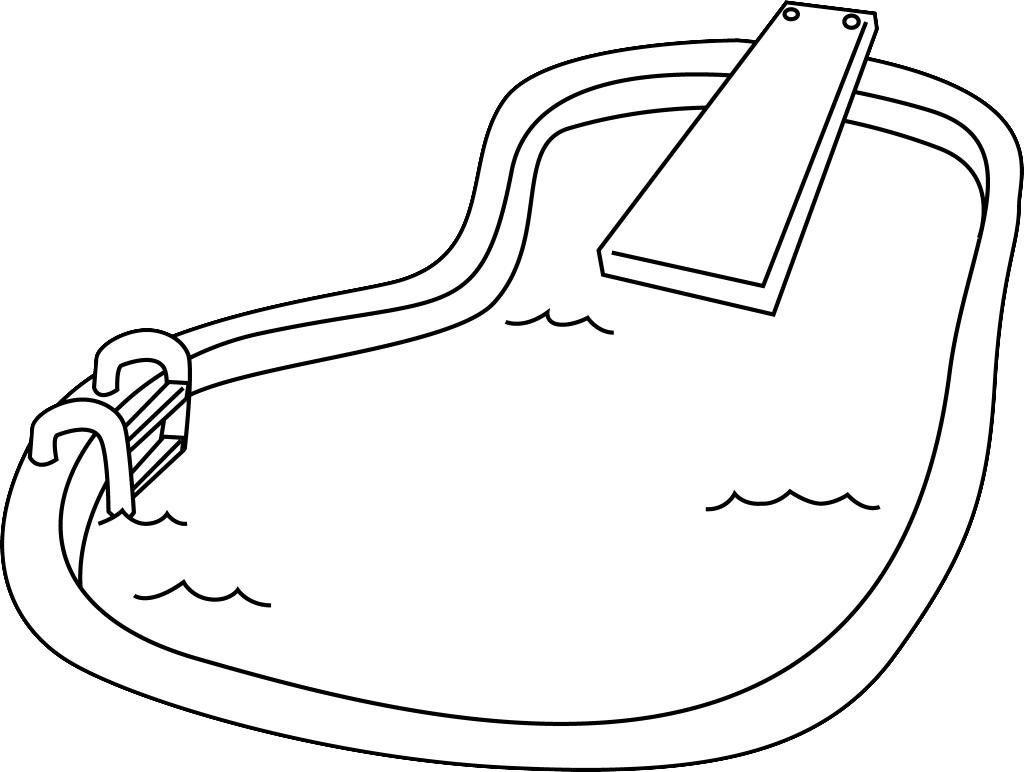
\includegraphics[width=0.4\textwidth]{figs/frontpage/smartpool.png}
\end{minipage}

\vspace{\fill}
\begin{minipage}[l]{\textwidth}
\begin{tabu} to \textwidth{lX[l]}
\textbf{Dato}           &\today\\
\textbf{Vejleder}		&Vejleder navn\\
\end{tabu}
\end{minipage}

\vspace{10pt}
\begin{minipage}[l]{\textwidth}
\tabulinesep=25pt
\begin{tabu} to \textwidth{X[l]X[l]X[l]}
 \makebox[\linewidth]{\hrulefill}\newline Joachim Dam Andersen     \newline 201370248/IKT  
&\makebox[\linewidth]{\hrulefill}\newline Lasse Priebe             \newline 201370248/IKT 
&\makebox[\linewidth]{\hrulefill}\newline Emil Nyborg              \newline 201370248/IKT\\
 \makebox[\linewidth]{\hrulefill}\newline Bjørn Nørgaard Sørensen  \newline 201370248/IKT  
&\makebox[\linewidth]{\hrulefill}\newline Alex Justesen Karlsen    \newline 201370248/IKT 
&\makebox[\linewidth]{\hrulefill}\newline Joachim Händel Noer Wind \newline 201370248/IKT
\end{tabu}
\end{minipage}\clearpage

%% Abstract
% Initial setup
\markboth{RESUMÉ/ABSTRACT}{RESUMÉ/ABSTRACT}
\abstractintoc
\abstractcol
\setlength{\abstitleskip}{-18pt}

% Abstract
\begin{abstract}
Rapporten omhandler et 3. semesterprojekt fra Ingeniørhøjskolen Aarhus Universitet udarbejdet med henblik på at producere et system, som kan fungere som dosering- og sorteringsanlæg til tabletter. Systemet er tiltænkt brug i ældreplejen, som en måde hvorpå fejlmedicinering kan undgås, og tabletsortering kan klares automatisk. Ydermere vil systemet kunne gøre personale og pårørende opmærksomme på, at brugeren ikke har afhentet sine tabletter, indenfor et givet tidsrum. Dette skal formidles ved hjælp af en Android applikation. Systemet og serveren samarbejder om at kontrollerer, hvad der dispenseres til den specifikke bruger og hvornår. Denne kommunikation er ikke fuldt ud implementeret endnu. Systemet var oprindeligt tiltænkt brug i private hjem, men undervejs i processen er idéen ændret idet at fokus flyttes fra private hjem til brug i plejesektoren. 
Produktet kan på nuværende tidspunkt dosere et bestemt antal tabletter af én enkelt type. Systemet har på nuværende tidspunkt allerede implementeret muligheden for at udvide med ekstra dispenserer, og er derfor velegnet til videreudvikling. 
Til systemet er der implementeret en fungerende brugergrænseflade, som er testet med en brugervenlighedsundersøgelse, der ved adspørgelse af 15 studerende har påpeget adskillige muligheder for forbedring.
Under systemudviklingen er den største arbejdsindsats lagt i undersøgelse af teknologier og mulige løsningsforslag.
\end{abstract}

\begin{abstracten}
The report covers a third semesterproject from the Aarhus University School of Engineering. The goal is to produce a system that can function as a dispensing and sorting machine for pills. The system is intended for use in eldercare, as a way of preventing medication errors and a way of sorting pills automaticly. Furthermore, the system will be able to notify staff and relatives if the elder has not picked up their pills, within a given timeperiod. The staff and relatives will be notified via an Android application. The system and a server operate together in order to control what is dispensed to whom and when. Though this communication is not fully implemented yet. The system was originally intended for use in private homes, but during the process, the idea evolved so that the focus was changed from home use to the healthcare sector.
The product can at this time dispense a certain number of pills which will have to be of a single type. The option of adding extra dispensers is already implemented, and is therefore suitable for further development.
The system also has a functioning interface implemented, which has been tested with a user-experience study in which 15 students participated. With the feedback made several things clear, and several of these are suitable for further work.
During the system development the largest effort was put into the study of technologies and potential solutions for the problem chosen.
\end{abstracten}\clearpage

%% Forord
\pagestyle{asereport}
\chapter{Forord}

% Forordet benyttes til at informere kort om visse ydre omstændigheder for projektet, såsom projekttype og hvor projektet er gennemført, historisk baggrund (andre arbejder, som har givet anledning til det aktuelle projekt) og hvor inspirationen og ideen er kommet fra, m.v.

Dette dokument er sammensat for at dokumentere arbejdet på 4. semesterprojektet for retningen IKT på ingeniørhøjskolen Århus.

Der vil i denne rapport være referencer til bilag og dokumentation, som det ikke ville være hensigtsmæssigt at medtage. Samtlige bilag m.m. vil være at finde på den vedlagt CD-rom. 

Source kode til projektet kan findes på CD'en. Link til vores github repo følger her: \newline \url{https://github.com/BjornNorgaard/DuckMaster3001}

\vspace{5mm}

\large{\textit{En stor tak til}}

\begin{displayquote}
    Lars Mortensen for god og brugbar vejledning.
\end{displayquote}

\begin{displayquote}
    Stjerne Apoteket for at lade gruppen komme på besøg og se deres sorteringsmaskine.
\end{displayquote}

\begin{displayquote}
    Sofie Fredslund for at lade os interviewe hende til projektet.
\end{displayquote}

\begin{displayquote}
   Underviserne på ASE, for hjælp og vejledning.
\end{displayquote}

\clearpage

%% ToC
\tableofcontents\clearpage

\mainmatter

%% Todo oversigt - SKAL UDKOMMENTERES FØR AFLEVERING
\listoftodos[Liste over gøremål]

%% Indledning
\chapter{Indledning}

Hello \cite{fysikbog} og sådan kan det jo gå.\clearpage

%% Projektformulering
\documentclass[a4paper,11pt,oneside]{memoir}
\input{utils/packages}
\input{utils/layout}
\input{utils/listings}
\input{utils/ordliste}

%% Forside variabler
\newcommand{\Kursus}{I4PRJ4 F16}
\newcommand{\Projektnavn}{SmartPool 2.0}
\newcommand{\Gruppe}{Gruppe 3}
\newcommand{\Projektdokument}{Projektrapport}

%% Litteratur
\nocite{*}
%\bibliographystyle{harvard}
\bibliography{utils/litteratur}

\begin{document}
\frontmatter

\input{utils/frontpage}\clearpage

%% Abstract
\input{docs/frontmatter/abstract}\clearpage

%% Forord
\pagestyle{asereport}
\input{docs/frontmatter/forord}\clearpage

%% ToC
\tableofcontents\clearpage

\mainmatter

%% Todo oversigt - SKAL UDKOMMENTERES FØR AFLEVERING
\listoftodos[Liste over gøremål]

%% Indledning
\input{docs/frontmatter/indledning}\clearpage

%% Projektformulering
\input{docs/projektformulering/main}\clearpage

%% Kravspecifikation
\input{docs/kravspecifikation/main}\clearpage

%% Systemarkitektur
\input{docs/systemarkitektur/main}\clearpage

%% Processbeskrivelse
\input{docs/processbeskrivelse/main}\clearpage

%% Design
\input{docs/design/main}\clearpage

%% Implementering
\input{docs/implementering/main}\clearpage

%% Integration
\input{docs/integration/main}\clearpage

%% Accepttest
\input{docs/accepttest/main}\clearpage

%% Appendix
\input{docs/appendix/main}\clearpage

\backmatter
%% Glossary
\setglossarystyle{list}
\printnoidxglossary[title=Ordliste]

% Bibliography
\clearpage
\printbibliography[title={Litteratur}]
\end{document}\clearpage

%% Kravspecifikation
\documentclass[a4paper,11pt,oneside]{memoir}
\input{utils/packages}
\input{utils/layout}
\input{utils/listings}
\input{utils/ordliste}

%% Forside variabler
\newcommand{\Kursus}{I4PRJ4 F16}
\newcommand{\Projektnavn}{SmartPool 2.0}
\newcommand{\Gruppe}{Gruppe 3}
\newcommand{\Projektdokument}{Projektrapport}

%% Litteratur
\nocite{*}
%\bibliographystyle{harvard}
\bibliography{utils/litteratur}

\begin{document}
\frontmatter

\input{utils/frontpage}\clearpage

%% Abstract
\input{docs/frontmatter/abstract}\clearpage

%% Forord
\pagestyle{asereport}
\input{docs/frontmatter/forord}\clearpage

%% ToC
\tableofcontents\clearpage

\mainmatter

%% Todo oversigt - SKAL UDKOMMENTERES FØR AFLEVERING
\listoftodos[Liste over gøremål]

%% Indledning
\input{docs/frontmatter/indledning}\clearpage

%% Projektformulering
\input{docs/projektformulering/main}\clearpage

%% Kravspecifikation
\input{docs/kravspecifikation/main}\clearpage

%% Systemarkitektur
\input{docs/systemarkitektur/main}\clearpage

%% Processbeskrivelse
\input{docs/processbeskrivelse/main}\clearpage

%% Design
\input{docs/design/main}\clearpage

%% Implementering
\input{docs/implementering/main}\clearpage

%% Integration
\input{docs/integration/main}\clearpage

%% Accepttest
\input{docs/accepttest/main}\clearpage

%% Appendix
\input{docs/appendix/main}\clearpage

\backmatter
%% Glossary
\setglossarystyle{list}
\printnoidxglossary[title=Ordliste]

% Bibliography
\clearpage
\printbibliography[title={Litteratur}]
\end{document}\clearpage

%% Systemarkitektur
\documentclass[a4paper,11pt,oneside]{memoir}
\input{utils/packages}
\input{utils/layout}
\input{utils/listings}
\input{utils/ordliste}

%% Forside variabler
\newcommand{\Kursus}{I4PRJ4 F16}
\newcommand{\Projektnavn}{SmartPool 2.0}
\newcommand{\Gruppe}{Gruppe 3}
\newcommand{\Projektdokument}{Projektrapport}

%% Litteratur
\nocite{*}
%\bibliographystyle{harvard}
\bibliography{utils/litteratur}

\begin{document}
\frontmatter

\input{utils/frontpage}\clearpage

%% Abstract
\input{docs/frontmatter/abstract}\clearpage

%% Forord
\pagestyle{asereport}
\input{docs/frontmatter/forord}\clearpage

%% ToC
\tableofcontents\clearpage

\mainmatter

%% Todo oversigt - SKAL UDKOMMENTERES FØR AFLEVERING
\listoftodos[Liste over gøremål]

%% Indledning
\input{docs/frontmatter/indledning}\clearpage

%% Projektformulering
\input{docs/projektformulering/main}\clearpage

%% Kravspecifikation
\input{docs/kravspecifikation/main}\clearpage

%% Systemarkitektur
\input{docs/systemarkitektur/main}\clearpage

%% Processbeskrivelse
\input{docs/processbeskrivelse/main}\clearpage

%% Design
\input{docs/design/main}\clearpage

%% Implementering
\input{docs/implementering/main}\clearpage

%% Integration
\input{docs/integration/main}\clearpage

%% Accepttest
\input{docs/accepttest/main}\clearpage

%% Appendix
\input{docs/appendix/main}\clearpage

\backmatter
%% Glossary
\setglossarystyle{list}
\printnoidxglossary[title=Ordliste]

% Bibliography
\clearpage
\printbibliography[title={Litteratur}]
\end{document}\clearpage

%% Processbeskrivelse
\documentclass[a4paper,11pt,oneside]{memoir}
\input{utils/packages}
\input{utils/layout}
\input{utils/listings}
\input{utils/ordliste}

%% Forside variabler
\newcommand{\Kursus}{I4PRJ4 F16}
\newcommand{\Projektnavn}{SmartPool 2.0}
\newcommand{\Gruppe}{Gruppe 3}
\newcommand{\Projektdokument}{Projektrapport}

%% Litteratur
\nocite{*}
%\bibliographystyle{harvard}
\bibliography{utils/litteratur}

\begin{document}
\frontmatter

\input{utils/frontpage}\clearpage

%% Abstract
\input{docs/frontmatter/abstract}\clearpage

%% Forord
\pagestyle{asereport}
\input{docs/frontmatter/forord}\clearpage

%% ToC
\tableofcontents\clearpage

\mainmatter

%% Todo oversigt - SKAL UDKOMMENTERES FØR AFLEVERING
\listoftodos[Liste over gøremål]

%% Indledning
\input{docs/frontmatter/indledning}\clearpage

%% Projektformulering
\input{docs/projektformulering/main}\clearpage

%% Kravspecifikation
\input{docs/kravspecifikation/main}\clearpage

%% Systemarkitektur
\input{docs/systemarkitektur/main}\clearpage

%% Processbeskrivelse
\input{docs/processbeskrivelse/main}\clearpage

%% Design
\input{docs/design/main}\clearpage

%% Implementering
\input{docs/implementering/main}\clearpage

%% Integration
\input{docs/integration/main}\clearpage

%% Accepttest
\input{docs/accepttest/main}\clearpage

%% Appendix
\input{docs/appendix/main}\clearpage

\backmatter
%% Glossary
\setglossarystyle{list}
\printnoidxglossary[title=Ordliste]

% Bibliography
\clearpage
\printbibliography[title={Litteratur}]
\end{document}\clearpage

%% Design
\documentclass[a4paper,11pt,oneside]{memoir}
\input{utils/packages}
\input{utils/layout}
\input{utils/listings}
\input{utils/ordliste}

%% Forside variabler
\newcommand{\Kursus}{I4PRJ4 F16}
\newcommand{\Projektnavn}{SmartPool 2.0}
\newcommand{\Gruppe}{Gruppe 3}
\newcommand{\Projektdokument}{Projektrapport}

%% Litteratur
\nocite{*}
%\bibliographystyle{harvard}
\bibliography{utils/litteratur}

\begin{document}
\frontmatter

\input{utils/frontpage}\clearpage

%% Abstract
\input{docs/frontmatter/abstract}\clearpage

%% Forord
\pagestyle{asereport}
\input{docs/frontmatter/forord}\clearpage

%% ToC
\tableofcontents\clearpage

\mainmatter

%% Todo oversigt - SKAL UDKOMMENTERES FØR AFLEVERING
\listoftodos[Liste over gøremål]

%% Indledning
\input{docs/frontmatter/indledning}\clearpage

%% Projektformulering
\input{docs/projektformulering/main}\clearpage

%% Kravspecifikation
\input{docs/kravspecifikation/main}\clearpage

%% Systemarkitektur
\input{docs/systemarkitektur/main}\clearpage

%% Processbeskrivelse
\input{docs/processbeskrivelse/main}\clearpage

%% Design
\input{docs/design/main}\clearpage

%% Implementering
\input{docs/implementering/main}\clearpage

%% Integration
\input{docs/integration/main}\clearpage

%% Accepttest
\input{docs/accepttest/main}\clearpage

%% Appendix
\input{docs/appendix/main}\clearpage

\backmatter
%% Glossary
\setglossarystyle{list}
\printnoidxglossary[title=Ordliste]

% Bibliography
\clearpage
\printbibliography[title={Litteratur}]
\end{document}\clearpage

%% Implementering
\documentclass[a4paper,11pt,oneside]{memoir}
\input{utils/packages}
\input{utils/layout}
\input{utils/listings}
\input{utils/ordliste}

%% Forside variabler
\newcommand{\Kursus}{I4PRJ4 F16}
\newcommand{\Projektnavn}{SmartPool 2.0}
\newcommand{\Gruppe}{Gruppe 3}
\newcommand{\Projektdokument}{Projektrapport}

%% Litteratur
\nocite{*}
%\bibliographystyle{harvard}
\bibliography{utils/litteratur}

\begin{document}
\frontmatter

\input{utils/frontpage}\clearpage

%% Abstract
\input{docs/frontmatter/abstract}\clearpage

%% Forord
\pagestyle{asereport}
\input{docs/frontmatter/forord}\clearpage

%% ToC
\tableofcontents\clearpage

\mainmatter

%% Todo oversigt - SKAL UDKOMMENTERES FØR AFLEVERING
\listoftodos[Liste over gøremål]

%% Indledning
\input{docs/frontmatter/indledning}\clearpage

%% Projektformulering
\input{docs/projektformulering/main}\clearpage

%% Kravspecifikation
\input{docs/kravspecifikation/main}\clearpage

%% Systemarkitektur
\input{docs/systemarkitektur/main}\clearpage

%% Processbeskrivelse
\input{docs/processbeskrivelse/main}\clearpage

%% Design
\input{docs/design/main}\clearpage

%% Implementering
\input{docs/implementering/main}\clearpage

%% Integration
\input{docs/integration/main}\clearpage

%% Accepttest
\input{docs/accepttest/main}\clearpage

%% Appendix
\input{docs/appendix/main}\clearpage

\backmatter
%% Glossary
\setglossarystyle{list}
\printnoidxglossary[title=Ordliste]

% Bibliography
\clearpage
\printbibliography[title={Litteratur}]
\end{document}\clearpage

%% Integration
\documentclass[a4paper,11pt,oneside]{memoir}
\input{utils/packages}
\input{utils/layout}
\input{utils/listings}
\input{utils/ordliste}

%% Forside variabler
\newcommand{\Kursus}{I4PRJ4 F16}
\newcommand{\Projektnavn}{SmartPool 2.0}
\newcommand{\Gruppe}{Gruppe 3}
\newcommand{\Projektdokument}{Projektrapport}

%% Litteratur
\nocite{*}
%\bibliographystyle{harvard}
\bibliography{utils/litteratur}

\begin{document}
\frontmatter

\input{utils/frontpage}\clearpage

%% Abstract
\input{docs/frontmatter/abstract}\clearpage

%% Forord
\pagestyle{asereport}
\input{docs/frontmatter/forord}\clearpage

%% ToC
\tableofcontents\clearpage

\mainmatter

%% Todo oversigt - SKAL UDKOMMENTERES FØR AFLEVERING
\listoftodos[Liste over gøremål]

%% Indledning
\input{docs/frontmatter/indledning}\clearpage

%% Projektformulering
\input{docs/projektformulering/main}\clearpage

%% Kravspecifikation
\input{docs/kravspecifikation/main}\clearpage

%% Systemarkitektur
\input{docs/systemarkitektur/main}\clearpage

%% Processbeskrivelse
\input{docs/processbeskrivelse/main}\clearpage

%% Design
\input{docs/design/main}\clearpage

%% Implementering
\input{docs/implementering/main}\clearpage

%% Integration
\input{docs/integration/main}\clearpage

%% Accepttest
\input{docs/accepttest/main}\clearpage

%% Appendix
\input{docs/appendix/main}\clearpage

\backmatter
%% Glossary
\setglossarystyle{list}
\printnoidxglossary[title=Ordliste]

% Bibliography
\clearpage
\printbibliography[title={Litteratur}]
\end{document}\clearpage

%% Accepttest
\documentclass[a4paper,11pt,oneside]{memoir}
\input{utils/packages}
\input{utils/layout}
\input{utils/listings}
\input{utils/ordliste}

%% Forside variabler
\newcommand{\Kursus}{I4PRJ4 F16}
\newcommand{\Projektnavn}{SmartPool 2.0}
\newcommand{\Gruppe}{Gruppe 3}
\newcommand{\Projektdokument}{Projektrapport}

%% Litteratur
\nocite{*}
%\bibliographystyle{harvard}
\bibliography{utils/litteratur}

\begin{document}
\frontmatter

\input{utils/frontpage}\clearpage

%% Abstract
\input{docs/frontmatter/abstract}\clearpage

%% Forord
\pagestyle{asereport}
\input{docs/frontmatter/forord}\clearpage

%% ToC
\tableofcontents\clearpage

\mainmatter

%% Todo oversigt - SKAL UDKOMMENTERES FØR AFLEVERING
\listoftodos[Liste over gøremål]

%% Indledning
\input{docs/frontmatter/indledning}\clearpage

%% Projektformulering
\input{docs/projektformulering/main}\clearpage

%% Kravspecifikation
\input{docs/kravspecifikation/main}\clearpage

%% Systemarkitektur
\input{docs/systemarkitektur/main}\clearpage

%% Processbeskrivelse
\input{docs/processbeskrivelse/main}\clearpage

%% Design
\input{docs/design/main}\clearpage

%% Implementering
\input{docs/implementering/main}\clearpage

%% Integration
\input{docs/integration/main}\clearpage

%% Accepttest
\input{docs/accepttest/main}\clearpage

%% Appendix
\input{docs/appendix/main}\clearpage

\backmatter
%% Glossary
\setglossarystyle{list}
\printnoidxglossary[title=Ordliste]

% Bibliography
\clearpage
\printbibliography[title={Litteratur}]
\end{document}\clearpage

%% Appendix
\documentclass[a4paper,11pt,oneside]{memoir}
\input{utils/packages}
\input{utils/layout}
\input{utils/listings}
\input{utils/ordliste}

%% Forside variabler
\newcommand{\Kursus}{I4PRJ4 F16}
\newcommand{\Projektnavn}{SmartPool 2.0}
\newcommand{\Gruppe}{Gruppe 3}
\newcommand{\Projektdokument}{Projektrapport}

%% Litteratur
\nocite{*}
%\bibliographystyle{harvard}
\bibliography{utils/litteratur}

\begin{document}
\frontmatter

\input{utils/frontpage}\clearpage

%% Abstract
\input{docs/frontmatter/abstract}\clearpage

%% Forord
\pagestyle{asereport}
\input{docs/frontmatter/forord}\clearpage

%% ToC
\tableofcontents\clearpage

\mainmatter

%% Todo oversigt - SKAL UDKOMMENTERES FØR AFLEVERING
\listoftodos[Liste over gøremål]

%% Indledning
\input{docs/frontmatter/indledning}\clearpage

%% Projektformulering
\input{docs/projektformulering/main}\clearpage

%% Kravspecifikation
\input{docs/kravspecifikation/main}\clearpage

%% Systemarkitektur
\input{docs/systemarkitektur/main}\clearpage

%% Processbeskrivelse
\input{docs/processbeskrivelse/main}\clearpage

%% Design
\input{docs/design/main}\clearpage

%% Implementering
\input{docs/implementering/main}\clearpage

%% Integration
\input{docs/integration/main}\clearpage

%% Accepttest
\input{docs/accepttest/main}\clearpage

%% Appendix
\input{docs/appendix/main}\clearpage

\backmatter
%% Glossary
\setglossarystyle{list}
\printnoidxglossary[title=Ordliste]

% Bibliography
\clearpage
\printbibliography[title={Litteratur}]
\end{document}\clearpage

\backmatter
%% Glossary
\setglossarystyle{list}
\printnoidxglossary[title=Ordliste]

% Bibliography
\clearpage
\printbibliography[title={Litteratur}]
\end{document}\clearpage

%% Integration
\documentclass[a4paper,11pt,oneside]{memoir}
%!TEX root = main.tex
% Encoding
%\usepackage[utf8]{inputenc} % pdfLatex
\usepackage[T1]{fontenc}
\usepackage[danish]{babel}
\renewcommand{\danishhyphenmins}{22}
\usepackage[utf8]{inputenc} % æ ø å

% Date
\usepackage[ddmmyyyy]{datetime}
\renewcommand{\dateseparator}{.}

% Fonts
\usepackage{fourier}
\usepackage[scaled=0.8]{beramono}

% Math
\usepackage{amsmath,amssymb}
\usepackage{bm}
\usepackage{amsthm}
\usepackage{mathtools}

% Graphics
\usepackage[usenames,dvipsnames,table]{xcolor}
\usepackage{graphicx}
\usepackage{float}
%\usepackage[section]{placeins}
\usepackage{tikz}
\usepackage[pages=some]{background}
\usepackage{wrapfig}

% Listings & Tables
\usepackage{listings}
%\usepackage{pythontex}
\usepackage{enumitem}
\usepackage{tabu}
\usepackage{longtable}
\usepackage{multirow}
\usepackage{makecell}


% References & Quotes
%\usepackage[danish]{varioref}				% Muliggoer bl.a. krydshenvisninger med sidetal (\vref)
%\usepackage{nat}							% Udvidelse med naturvidenskabelige citationsmodeller
\usepackage[danish=guillemets]{csquotes}
\usepackage[hidelinks]{hyperref}
\hypersetup{
    pdfstartview={FitH},
    pdftitle={Smart Pool 2.0},
    pdfsubject={Projektrapport},
    pdfauthor={I4PRJ4GRP3}
}
\usepackage[all]{hypcap}

% Etc
\usepackage[
	%backend=biber,
	backend=bibtex,
	style=ieee,
	natbib=true,
	backref=false,
	backrefstyle=all+,
	hyperref=true
]{biblatex}
\usepackage{pdflscape}
\usepackage[nomain,toc,xindy,acronym,nonumberlist,noredefwarn]{glossaries}
\usepackage[xindy]{imakeidx}
\usepackage{float}
\makeindex

% Dummy
\usepackage{lipsum}
%!TEX root = main.tex
% Page setup
\setulmarginsandblock{35mm}{25mm}{*}
\setlrmarginsandblock{20mm}{20mm}{*}
\setheadfoot{4\onelineskip}{2\onelineskip}
\setheaderspaces{*}{5mm}{*}
\checkandfixthelayout

% Pagestyle
\makepagestyle{asereport}
	\makeevenhead{asereport}{}{}{}
	\makeoddhead{asereport}{
\includegraphics{figs/frontpage/aseaulogo.pdf}}{}{\small\rightmark{} | \textbf{\thepage{}\vspace{7pt}}}
	\makeevenfoot{asereport}{}{}{}
	\makeoddfoot{asereport}{}{}{}

\makepsmarks{asereport}{
	\createmark{chapter}{both}{shownumber}{}{. \ }
	\createmark{section}{both}{shownumber}{}{. \ }
	\createmark{subsection}{both}{shownumber}{}{. \ }
	\createplainmark{toc}{both}{\contentsname}
	\createplainmark{lof}{both}{\listfigurename}
	\createplainmark{lot}{both}{\listtablename}
	\createplainmark{bib}{both}{\bibname}
	\createplainmark{index}{both}{\indexname}
	\createplainmark{glossary}{both}{\glossaryname}
}

\aliaspagestyle{part}{asereport}
\aliaspagestyle{chapter}{asereport}
\chapterstyle{tandh}

% Modification to certain spacing
\setlength{\parskip}{8pt}
\setlength{\parindent}{0pt}
\setlength{\abovecaptionskip}{7pt}
\setlength{\belowcaptionskip}{-10pt}
\OnehalfSpacing

% Tabu
%\taburowcolors[1]2{white .. light-gray}
\tabulinesep=4pt

% Itemize/enumerate
\setlist{
    before=\vspace{-3pt}, 
    after=\vspace{-3pt},
    itemsep=0pt,
    leftmargin=25pt,
    labelsep=10pt,
    topsep=0pt,
}

% Kommandoer til UC - fixer spacing
% Aktører
\newcommand{\fua}[1]{
	\begin{minipage}[t]{\linewidth}
		\setlist{
		    leftmargin=22pt,
		    itemsep=0pt,
		    topsep=0pt,
		    parsep=3pt
		}
	\begin{itemize}[before={\vspace{-6pt}}, after={\vspace{6pt}}]
	#1
	\end{itemize}
	\end{minipage}
}

% Hovedforløb
\newcommand{\fu}[1]{
\begin{minipage}[t]{\linewidth}
\setlist{
    leftmargin=22pt,
    itemsep=0pt,
    topsep=0pt,
    parsep=3pt
}
\raggedright
\begin{enumerate}[before={\vspace{-5pt}},after={\vspace{6pt}}]
#1
\end{enumerate}
\end{minipage}}

% Extensions
\newcommand{\fuex}[2]{
\begin{minipage}[t]{\linewidth}
\vspace{-6pt}
\raggedright
\textit{#1}
\begin{enumerate}[leftmargin=22pt,itemsep=0pt,parsep=3pt,before={\vspace{-8pt}}, after={\vspace{20pt}},topsep=8pt]
#2
\end{enumerate}
\end{minipage}
}

% Extensions - Sidste entry
\newcommand{\fuexl}[2]{
\begin{minipage}[t]{\linewidth}
\vspace{-6pt}
\raggedright
\textit{#1}
\begin{enumerate}[leftmargin=22pt,itemsep=0pt,parsep=3pt,before={\vspace{-8pt}}, after={\vspace{3pt}},topsep=8pt]
#2
\end{enumerate}
\end{minipage}}

% Versionshistorik
\newcommand{\verhistitem}[2]{
\begin{minipage}[t]{\linewidth}
\vspace{-6pt}
\raggedright
#1
\begin{itemize}[leftmargin=22pt,itemsep=0pt,parsep=0pt,before={\vspace{-10pt}},after={\vspace{3pt}},topsep=8pt]
#2
\end{itemize}
\end{minipage}}

\newcommand{\tverb}[1]{{\texttt{#1}}}

\newcommand{\cond}[1]{
\begin{itemize}[label=,noitemsep,topsep=0pt,after={\vspace*{-\baselineskip}}]
#1
\end{itemize}}

% Etc
\definecolor{light-gray}{gray}{0.8}
\definecolor{pantone}{RGB}{0,61,133}

\setfloatlocations{figure}{H}
\setfloatlocations{table}{H}

\numberwithin{equation}{chapter}
\numberwithin{figure}{chapter}
\setcounter{secnumdepth}{3}
\setcounter{tocdepth}{2}
\maxsecnumdepth{subsection}

\renewcommand*{\cftdotsep}{1}
\setpnumwidth{2em}
\setrmarg{2em}

\setverbatimfont{\ttfamily}

%\renewcommand\cftchaptername {\chaptername~}
%\renewcommand\cftappendixname {\appendixname~}
\addto\captionsdanish{
    \renewcommand\contentsname{Indholdsfortegnelse}
    \renewcommand\appendixname{Appendiks}
}
\renewcommand\appendixpagename{Appendiks}
\renewcommand\appendixtocname{Appendiks}
\newsubfloat{figure}

% Abstract
\newenvironment{abstracten}
{\renewcommand{\abstractname}{Abstract}\abstract}
{\endabstract}
\renewcommand{\abstractnamefont}{\normalfont\Large\bfseries}
%!TEX root = main.tex
% Listings
\AtBeginDocument{%
  \counterwithin*{lstlisting}{section}
  \counterwithin*{lstlisting}{subsection}
  \counterwithin*{lstlisting}{subsubsection}
  \renewcommand{\thelstlisting}{%
    \ifnum\value{subsection}=0
      \thesection.\arabic{lstlisting}%
    \else
      \ifnum\value{subsubsection}=0
        \thesubsection.\arabic{lstlisting}%
      \else
        \thesubsubsection.\arabic{lstlisting}%
      \fi
    \fi
  }
}

% Loading languages
\lstloadlanguages{C, C++}

% Listing setup
\lstdefinestyle{all}{
    basicstyle    = \ttfamily\SingleSpacing\scriptsize,
    numbers       = left, 
    numberstyle   = \ttfamily\tiny,
    breaklines    = true,
    commentstyle=\color{green},
    %backgroundcolor = \color{red},
    numbersep     = 20pt,
    xleftmargin   = \parindent,
    captionpos    = b,
    keywordstyle  = [1]\color{Blue}\bfseries,
    commentstyle  = \itshape\color{Green},
    tabsize       = 3
}

\lstset{
    style = all
} 
%!TEX root = main.tex
\makenoidxglossaries
\newglossaryentry{gui}{
    name={GUI}, 
    description={Graphical User Interface er en brugergrænseflade. Brugerens måde at tilgå systemet på}}

\newglossaryentry{psoc}{
    name={PSoC}, 
    description={PSoC (Programmable System-on-Chip) er et microcontroller system produceret af Cypress Semiconductor}}

\newglossaryentry{moscow}{
    name={MoSCoW}, 
    description={MoSCoW er en metode til at prioritere krav til ens system}}

\newglossaryentry{furps}{
    name={FURPS}, 
    description={FURPS er en metode til kategorisering af systemets ikke-funktionelle krav}}

\newglossaryentry{BDD}{
    name={BDD}, 
    description={BDD (Block Definition Diagram) er et diagram, som beskriver et system ved at opdele det op i mindre blokke}}

\newglossaryentry{IBD}{
    name={IBD}, 
    description={IBD (Internal Block Diagram) er et diagram, som viser forbindelserne mellem blokkene, som kan findes i et BDD}}

\newglossaryentry{pilleskuffe}{
    name={Pilleskuffe},
    description={Skuffen under dispenseren, hvor i den nederste pille ligger i. Skuffen tømmes ved at elektromagneten trækker skuffen til sig.}}

\newglossaryentry{pilledispenser}{
    name={Pilledispenser},
    description={Det rør som pillerne bliver opbevaret i.}}

\newglossaryentry{elektromagneten}{
    name={Elektromagneten},
    description={Elektromagneten er en spole der sendes strøm igennem. Når der er strøm på spolen dannes et magnetfelt. Der vil ofte være tale om det samme hvad enten der står spole eller elektromagnet.}}

%% Forside variabler
\newcommand{\Kursus}{I4PRJ4 F16}
\newcommand{\Projektnavn}{SmartPool 2.0}
\newcommand{\Gruppe}{Gruppe 3}
\newcommand{\Projektdokument}{Projektrapport}

%% Litteratur
\nocite{*}
%\bibliographystyle{harvard}
\bibliography{utils/litteratur}

\begin{document}
\frontmatter

%!TEX root = main.tex
\pagestyle{titlingpage}
\backgroundsetup{
	scale=1,
	angle=0,
	opacity=1,
	contents={
		\begin{tikzpicture}[remember picture,overlay]
		\path [fill=pantone] (-0.5\paperwidth,0.36\paperheight) rectangle (0.5\paperwidth,0.47\paperheight);  
		\path [fill=pantone] (-0.5\paperwidth,-0.47\paperheight) rectangle (0.5\paperwidth,-0.43\paperheight);  
		\end{tikzpicture}}}
\BgThispage
\vspace*{-25mm}
\begin{minipage}[l]{\textwidth}
	
\includegraphics[width=0.75\textwidth]{figs/frontpage/aseaulogohvid.pdf}
\end{minipage}

\vspace{35pt}
\begin{minipage}[l]{\textwidth}
\tabulinesep=10pt
\begin{tabu} to \textwidth{X[l]}
	{\small\MakeUppercase\Kursus}\\
	{\HUGE\bfseries\MakeUppercase\Projektnavn}\\
	{\Large\Gruppe}\\
	{\itshape\Projektdokument}
\end{tabu}
\end{minipage}

\vspace{5pt}
\begin{minipage}[l]{\textwidth}
    \centering
	\vspace*{0cm}\hspace*{8cm}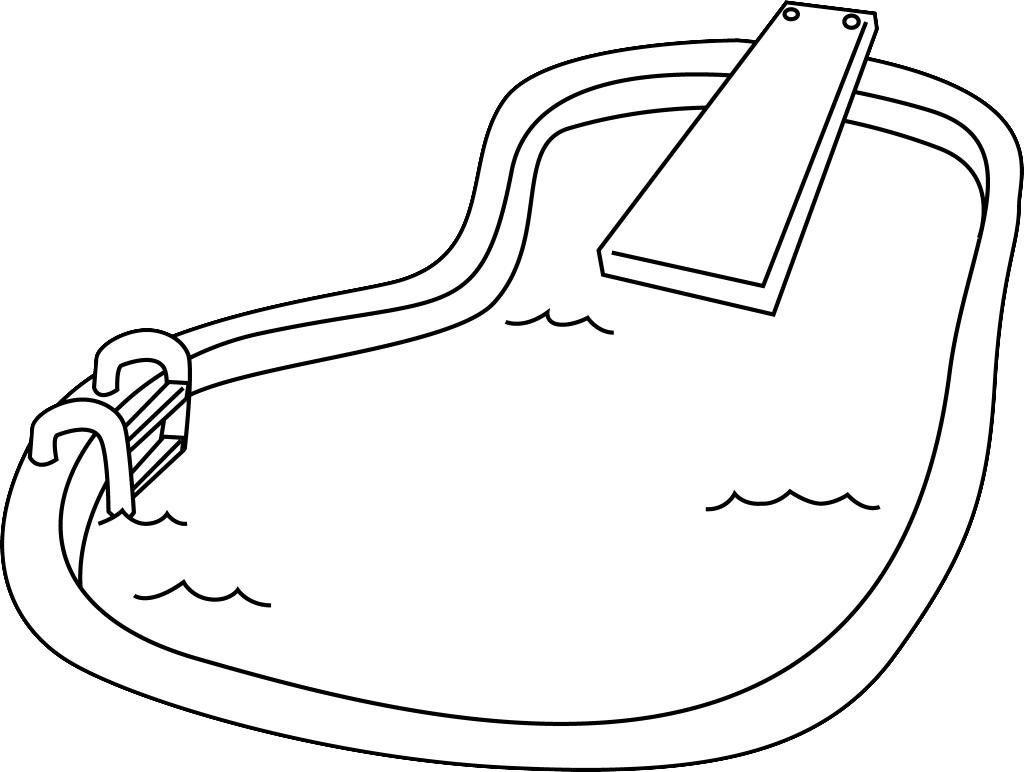
\includegraphics[width=0.4\textwidth]{figs/frontpage/smartpool.png}
\end{minipage}

\vspace{\fill}
\begin{minipage}[l]{\textwidth}
\begin{tabu} to \textwidth{lX[l]}
\textbf{Dato}           &\today\\
\textbf{Vejleder}		&Vejleder navn\\
\end{tabu}
\end{minipage}

\vspace{10pt}
\begin{minipage}[l]{\textwidth}
\tabulinesep=25pt
\begin{tabu} to \textwidth{X[l]X[l]X[l]}
 \makebox[\linewidth]{\hrulefill}\newline Joachim Dam Andersen     \newline 201370248/IKT  
&\makebox[\linewidth]{\hrulefill}\newline Lasse Priebe             \newline 201370248/IKT 
&\makebox[\linewidth]{\hrulefill}\newline Emil Nyborg              \newline 201370248/IKT\\
 \makebox[\linewidth]{\hrulefill}\newline Bjørn Nørgaard Sørensen  \newline 201370248/IKT  
&\makebox[\linewidth]{\hrulefill}\newline Alex Justesen Karlsen    \newline 201370248/IKT 
&\makebox[\linewidth]{\hrulefill}\newline Joachim Händel Noer Wind \newline 201370248/IKT
\end{tabu}
\end{minipage}\clearpage

%% Abstract
% Initial setup
\markboth{RESUMÉ/ABSTRACT}{RESUMÉ/ABSTRACT}
\abstractintoc
\abstractcol
\setlength{\abstitleskip}{-18pt}

% Abstract
\begin{abstract}
Rapporten omhandler et 3. semesterprojekt fra Ingeniørhøjskolen Aarhus Universitet udarbejdet med henblik på at producere et system, som kan fungere som dosering- og sorteringsanlæg til tabletter. Systemet er tiltænkt brug i ældreplejen, som en måde hvorpå fejlmedicinering kan undgås, og tabletsortering kan klares automatisk. Ydermere vil systemet kunne gøre personale og pårørende opmærksomme på, at brugeren ikke har afhentet sine tabletter, indenfor et givet tidsrum. Dette skal formidles ved hjælp af en Android applikation. Systemet og serveren samarbejder om at kontrollerer, hvad der dispenseres til den specifikke bruger og hvornår. Denne kommunikation er ikke fuldt ud implementeret endnu. Systemet var oprindeligt tiltænkt brug i private hjem, men undervejs i processen er idéen ændret idet at fokus flyttes fra private hjem til brug i plejesektoren. 
Produktet kan på nuværende tidspunkt dosere et bestemt antal tabletter af én enkelt type. Systemet har på nuværende tidspunkt allerede implementeret muligheden for at udvide med ekstra dispenserer, og er derfor velegnet til videreudvikling. 
Til systemet er der implementeret en fungerende brugergrænseflade, som er testet med en brugervenlighedsundersøgelse, der ved adspørgelse af 15 studerende har påpeget adskillige muligheder for forbedring.
Under systemudviklingen er den største arbejdsindsats lagt i undersøgelse af teknologier og mulige løsningsforslag.
\end{abstract}

\begin{abstracten}
The report covers a third semesterproject from the Aarhus University School of Engineering. The goal is to produce a system that can function as a dispensing and sorting machine for pills. The system is intended for use in eldercare, as a way of preventing medication errors and a way of sorting pills automaticly. Furthermore, the system will be able to notify staff and relatives if the elder has not picked up their pills, within a given timeperiod. The staff and relatives will be notified via an Android application. The system and a server operate together in order to control what is dispensed to whom and when. Though this communication is not fully implemented yet. The system was originally intended for use in private homes, but during the process, the idea evolved so that the focus was changed from home use to the healthcare sector.
The product can at this time dispense a certain number of pills which will have to be of a single type. The option of adding extra dispensers is already implemented, and is therefore suitable for further development.
The system also has a functioning interface implemented, which has been tested with a user-experience study in which 15 students participated. With the feedback made several things clear, and several of these are suitable for further work.
During the system development the largest effort was put into the study of technologies and potential solutions for the problem chosen.
\end{abstracten}\clearpage

%% Forord
\pagestyle{asereport}
\chapter{Forord}

% Forordet benyttes til at informere kort om visse ydre omstændigheder for projektet, såsom projekttype og hvor projektet er gennemført, historisk baggrund (andre arbejder, som har givet anledning til det aktuelle projekt) og hvor inspirationen og ideen er kommet fra, m.v.

Dette dokument er sammensat for at dokumentere arbejdet på 4. semesterprojektet for retningen IKT på ingeniørhøjskolen Århus.

Der vil i denne rapport være referencer til bilag og dokumentation, som det ikke ville være hensigtsmæssigt at medtage. Samtlige bilag m.m. vil være at finde på den vedlagt CD-rom. 

Source kode til projektet kan findes på CD'en. Link til vores github repo følger her: \newline \url{https://github.com/BjornNorgaard/DuckMaster3001}

\vspace{5mm}

\large{\textit{En stor tak til}}

\begin{displayquote}
    Lars Mortensen for god og brugbar vejledning.
\end{displayquote}

\begin{displayquote}
    Stjerne Apoteket for at lade gruppen komme på besøg og se deres sorteringsmaskine.
\end{displayquote}

\begin{displayquote}
    Sofie Fredslund for at lade os interviewe hende til projektet.
\end{displayquote}

\begin{displayquote}
   Underviserne på ASE, for hjælp og vejledning.
\end{displayquote}

\clearpage

%% ToC
\tableofcontents\clearpage

\mainmatter

%% Todo oversigt - SKAL UDKOMMENTERES FØR AFLEVERING
\listoftodos[Liste over gøremål]

%% Indledning
\chapter{Indledning}

Hello \cite{fysikbog} og sådan kan det jo gå.\clearpage

%% Projektformulering
\documentclass[a4paper,11pt,oneside]{memoir}
\input{utils/packages}
\input{utils/layout}
\input{utils/listings}
\input{utils/ordliste}

%% Forside variabler
\newcommand{\Kursus}{I4PRJ4 F16}
\newcommand{\Projektnavn}{SmartPool 2.0}
\newcommand{\Gruppe}{Gruppe 3}
\newcommand{\Projektdokument}{Projektrapport}

%% Litteratur
\nocite{*}
%\bibliographystyle{harvard}
\bibliography{utils/litteratur}

\begin{document}
\frontmatter

\input{utils/frontpage}\clearpage

%% Abstract
\input{docs/frontmatter/abstract}\clearpage

%% Forord
\pagestyle{asereport}
\input{docs/frontmatter/forord}\clearpage

%% ToC
\tableofcontents\clearpage

\mainmatter

%% Todo oversigt - SKAL UDKOMMENTERES FØR AFLEVERING
\listoftodos[Liste over gøremål]

%% Indledning
\input{docs/frontmatter/indledning}\clearpage

%% Projektformulering
\input{docs/projektformulering/main}\clearpage

%% Kravspecifikation
\input{docs/kravspecifikation/main}\clearpage

%% Systemarkitektur
\input{docs/systemarkitektur/main}\clearpage

%% Processbeskrivelse
\input{docs/processbeskrivelse/main}\clearpage

%% Design
\input{docs/design/main}\clearpage

%% Implementering
\input{docs/implementering/main}\clearpage

%% Integration
\input{docs/integration/main}\clearpage

%% Accepttest
\input{docs/accepttest/main}\clearpage

%% Appendix
\input{docs/appendix/main}\clearpage

\backmatter
%% Glossary
\setglossarystyle{list}
\printnoidxglossary[title=Ordliste]

% Bibliography
\clearpage
\printbibliography[title={Litteratur}]
\end{document}\clearpage

%% Kravspecifikation
\documentclass[a4paper,11pt,oneside]{memoir}
\input{utils/packages}
\input{utils/layout}
\input{utils/listings}
\input{utils/ordliste}

%% Forside variabler
\newcommand{\Kursus}{I4PRJ4 F16}
\newcommand{\Projektnavn}{SmartPool 2.0}
\newcommand{\Gruppe}{Gruppe 3}
\newcommand{\Projektdokument}{Projektrapport}

%% Litteratur
\nocite{*}
%\bibliographystyle{harvard}
\bibliography{utils/litteratur}

\begin{document}
\frontmatter

\input{utils/frontpage}\clearpage

%% Abstract
\input{docs/frontmatter/abstract}\clearpage

%% Forord
\pagestyle{asereport}
\input{docs/frontmatter/forord}\clearpage

%% ToC
\tableofcontents\clearpage

\mainmatter

%% Todo oversigt - SKAL UDKOMMENTERES FØR AFLEVERING
\listoftodos[Liste over gøremål]

%% Indledning
\input{docs/frontmatter/indledning}\clearpage

%% Projektformulering
\input{docs/projektformulering/main}\clearpage

%% Kravspecifikation
\input{docs/kravspecifikation/main}\clearpage

%% Systemarkitektur
\input{docs/systemarkitektur/main}\clearpage

%% Processbeskrivelse
\input{docs/processbeskrivelse/main}\clearpage

%% Design
\input{docs/design/main}\clearpage

%% Implementering
\input{docs/implementering/main}\clearpage

%% Integration
\input{docs/integration/main}\clearpage

%% Accepttest
\input{docs/accepttest/main}\clearpage

%% Appendix
\input{docs/appendix/main}\clearpage

\backmatter
%% Glossary
\setglossarystyle{list}
\printnoidxglossary[title=Ordliste]

% Bibliography
\clearpage
\printbibliography[title={Litteratur}]
\end{document}\clearpage

%% Systemarkitektur
\documentclass[a4paper,11pt,oneside]{memoir}
\input{utils/packages}
\input{utils/layout}
\input{utils/listings}
\input{utils/ordliste}

%% Forside variabler
\newcommand{\Kursus}{I4PRJ4 F16}
\newcommand{\Projektnavn}{SmartPool 2.0}
\newcommand{\Gruppe}{Gruppe 3}
\newcommand{\Projektdokument}{Projektrapport}

%% Litteratur
\nocite{*}
%\bibliographystyle{harvard}
\bibliography{utils/litteratur}

\begin{document}
\frontmatter

\input{utils/frontpage}\clearpage

%% Abstract
\input{docs/frontmatter/abstract}\clearpage

%% Forord
\pagestyle{asereport}
\input{docs/frontmatter/forord}\clearpage

%% ToC
\tableofcontents\clearpage

\mainmatter

%% Todo oversigt - SKAL UDKOMMENTERES FØR AFLEVERING
\listoftodos[Liste over gøremål]

%% Indledning
\input{docs/frontmatter/indledning}\clearpage

%% Projektformulering
\input{docs/projektformulering/main}\clearpage

%% Kravspecifikation
\input{docs/kravspecifikation/main}\clearpage

%% Systemarkitektur
\input{docs/systemarkitektur/main}\clearpage

%% Processbeskrivelse
\input{docs/processbeskrivelse/main}\clearpage

%% Design
\input{docs/design/main}\clearpage

%% Implementering
\input{docs/implementering/main}\clearpage

%% Integration
\input{docs/integration/main}\clearpage

%% Accepttest
\input{docs/accepttest/main}\clearpage

%% Appendix
\input{docs/appendix/main}\clearpage

\backmatter
%% Glossary
\setglossarystyle{list}
\printnoidxglossary[title=Ordliste]

% Bibliography
\clearpage
\printbibliography[title={Litteratur}]
\end{document}\clearpage

%% Processbeskrivelse
\documentclass[a4paper,11pt,oneside]{memoir}
\input{utils/packages}
\input{utils/layout}
\input{utils/listings}
\input{utils/ordliste}

%% Forside variabler
\newcommand{\Kursus}{I4PRJ4 F16}
\newcommand{\Projektnavn}{SmartPool 2.0}
\newcommand{\Gruppe}{Gruppe 3}
\newcommand{\Projektdokument}{Projektrapport}

%% Litteratur
\nocite{*}
%\bibliographystyle{harvard}
\bibliography{utils/litteratur}

\begin{document}
\frontmatter

\input{utils/frontpage}\clearpage

%% Abstract
\input{docs/frontmatter/abstract}\clearpage

%% Forord
\pagestyle{asereport}
\input{docs/frontmatter/forord}\clearpage

%% ToC
\tableofcontents\clearpage

\mainmatter

%% Todo oversigt - SKAL UDKOMMENTERES FØR AFLEVERING
\listoftodos[Liste over gøremål]

%% Indledning
\input{docs/frontmatter/indledning}\clearpage

%% Projektformulering
\input{docs/projektformulering/main}\clearpage

%% Kravspecifikation
\input{docs/kravspecifikation/main}\clearpage

%% Systemarkitektur
\input{docs/systemarkitektur/main}\clearpage

%% Processbeskrivelse
\input{docs/processbeskrivelse/main}\clearpage

%% Design
\input{docs/design/main}\clearpage

%% Implementering
\input{docs/implementering/main}\clearpage

%% Integration
\input{docs/integration/main}\clearpage

%% Accepttest
\input{docs/accepttest/main}\clearpage

%% Appendix
\input{docs/appendix/main}\clearpage

\backmatter
%% Glossary
\setglossarystyle{list}
\printnoidxglossary[title=Ordliste]

% Bibliography
\clearpage
\printbibliography[title={Litteratur}]
\end{document}\clearpage

%% Design
\documentclass[a4paper,11pt,oneside]{memoir}
\input{utils/packages}
\input{utils/layout}
\input{utils/listings}
\input{utils/ordliste}

%% Forside variabler
\newcommand{\Kursus}{I4PRJ4 F16}
\newcommand{\Projektnavn}{SmartPool 2.0}
\newcommand{\Gruppe}{Gruppe 3}
\newcommand{\Projektdokument}{Projektrapport}

%% Litteratur
\nocite{*}
%\bibliographystyle{harvard}
\bibliography{utils/litteratur}

\begin{document}
\frontmatter

\input{utils/frontpage}\clearpage

%% Abstract
\input{docs/frontmatter/abstract}\clearpage

%% Forord
\pagestyle{asereport}
\input{docs/frontmatter/forord}\clearpage

%% ToC
\tableofcontents\clearpage

\mainmatter

%% Todo oversigt - SKAL UDKOMMENTERES FØR AFLEVERING
\listoftodos[Liste over gøremål]

%% Indledning
\input{docs/frontmatter/indledning}\clearpage

%% Projektformulering
\input{docs/projektformulering/main}\clearpage

%% Kravspecifikation
\input{docs/kravspecifikation/main}\clearpage

%% Systemarkitektur
\input{docs/systemarkitektur/main}\clearpage

%% Processbeskrivelse
\input{docs/processbeskrivelse/main}\clearpage

%% Design
\input{docs/design/main}\clearpage

%% Implementering
\input{docs/implementering/main}\clearpage

%% Integration
\input{docs/integration/main}\clearpage

%% Accepttest
\input{docs/accepttest/main}\clearpage

%% Appendix
\input{docs/appendix/main}\clearpage

\backmatter
%% Glossary
\setglossarystyle{list}
\printnoidxglossary[title=Ordliste]

% Bibliography
\clearpage
\printbibliography[title={Litteratur}]
\end{document}\clearpage

%% Implementering
\documentclass[a4paper,11pt,oneside]{memoir}
\input{utils/packages}
\input{utils/layout}
\input{utils/listings}
\input{utils/ordliste}

%% Forside variabler
\newcommand{\Kursus}{I4PRJ4 F16}
\newcommand{\Projektnavn}{SmartPool 2.0}
\newcommand{\Gruppe}{Gruppe 3}
\newcommand{\Projektdokument}{Projektrapport}

%% Litteratur
\nocite{*}
%\bibliographystyle{harvard}
\bibliography{utils/litteratur}

\begin{document}
\frontmatter

\input{utils/frontpage}\clearpage

%% Abstract
\input{docs/frontmatter/abstract}\clearpage

%% Forord
\pagestyle{asereport}
\input{docs/frontmatter/forord}\clearpage

%% ToC
\tableofcontents\clearpage

\mainmatter

%% Todo oversigt - SKAL UDKOMMENTERES FØR AFLEVERING
\listoftodos[Liste over gøremål]

%% Indledning
\input{docs/frontmatter/indledning}\clearpage

%% Projektformulering
\input{docs/projektformulering/main}\clearpage

%% Kravspecifikation
\input{docs/kravspecifikation/main}\clearpage

%% Systemarkitektur
\input{docs/systemarkitektur/main}\clearpage

%% Processbeskrivelse
\input{docs/processbeskrivelse/main}\clearpage

%% Design
\input{docs/design/main}\clearpage

%% Implementering
\input{docs/implementering/main}\clearpage

%% Integration
\input{docs/integration/main}\clearpage

%% Accepttest
\input{docs/accepttest/main}\clearpage

%% Appendix
\input{docs/appendix/main}\clearpage

\backmatter
%% Glossary
\setglossarystyle{list}
\printnoidxglossary[title=Ordliste]

% Bibliography
\clearpage
\printbibliography[title={Litteratur}]
\end{document}\clearpage

%% Integration
\documentclass[a4paper,11pt,oneside]{memoir}
\input{utils/packages}
\input{utils/layout}
\input{utils/listings}
\input{utils/ordliste}

%% Forside variabler
\newcommand{\Kursus}{I4PRJ4 F16}
\newcommand{\Projektnavn}{SmartPool 2.0}
\newcommand{\Gruppe}{Gruppe 3}
\newcommand{\Projektdokument}{Projektrapport}

%% Litteratur
\nocite{*}
%\bibliographystyle{harvard}
\bibliography{utils/litteratur}

\begin{document}
\frontmatter

\input{utils/frontpage}\clearpage

%% Abstract
\input{docs/frontmatter/abstract}\clearpage

%% Forord
\pagestyle{asereport}
\input{docs/frontmatter/forord}\clearpage

%% ToC
\tableofcontents\clearpage

\mainmatter

%% Todo oversigt - SKAL UDKOMMENTERES FØR AFLEVERING
\listoftodos[Liste over gøremål]

%% Indledning
\input{docs/frontmatter/indledning}\clearpage

%% Projektformulering
\input{docs/projektformulering/main}\clearpage

%% Kravspecifikation
\input{docs/kravspecifikation/main}\clearpage

%% Systemarkitektur
\input{docs/systemarkitektur/main}\clearpage

%% Processbeskrivelse
\input{docs/processbeskrivelse/main}\clearpage

%% Design
\input{docs/design/main}\clearpage

%% Implementering
\input{docs/implementering/main}\clearpage

%% Integration
\input{docs/integration/main}\clearpage

%% Accepttest
\input{docs/accepttest/main}\clearpage

%% Appendix
\input{docs/appendix/main}\clearpage

\backmatter
%% Glossary
\setglossarystyle{list}
\printnoidxglossary[title=Ordliste]

% Bibliography
\clearpage
\printbibliography[title={Litteratur}]
\end{document}\clearpage

%% Accepttest
\documentclass[a4paper,11pt,oneside]{memoir}
\input{utils/packages}
\input{utils/layout}
\input{utils/listings}
\input{utils/ordliste}

%% Forside variabler
\newcommand{\Kursus}{I4PRJ4 F16}
\newcommand{\Projektnavn}{SmartPool 2.0}
\newcommand{\Gruppe}{Gruppe 3}
\newcommand{\Projektdokument}{Projektrapport}

%% Litteratur
\nocite{*}
%\bibliographystyle{harvard}
\bibliography{utils/litteratur}

\begin{document}
\frontmatter

\input{utils/frontpage}\clearpage

%% Abstract
\input{docs/frontmatter/abstract}\clearpage

%% Forord
\pagestyle{asereport}
\input{docs/frontmatter/forord}\clearpage

%% ToC
\tableofcontents\clearpage

\mainmatter

%% Todo oversigt - SKAL UDKOMMENTERES FØR AFLEVERING
\listoftodos[Liste over gøremål]

%% Indledning
\input{docs/frontmatter/indledning}\clearpage

%% Projektformulering
\input{docs/projektformulering/main}\clearpage

%% Kravspecifikation
\input{docs/kravspecifikation/main}\clearpage

%% Systemarkitektur
\input{docs/systemarkitektur/main}\clearpage

%% Processbeskrivelse
\input{docs/processbeskrivelse/main}\clearpage

%% Design
\input{docs/design/main}\clearpage

%% Implementering
\input{docs/implementering/main}\clearpage

%% Integration
\input{docs/integration/main}\clearpage

%% Accepttest
\input{docs/accepttest/main}\clearpage

%% Appendix
\input{docs/appendix/main}\clearpage

\backmatter
%% Glossary
\setglossarystyle{list}
\printnoidxglossary[title=Ordliste]

% Bibliography
\clearpage
\printbibliography[title={Litteratur}]
\end{document}\clearpage

%% Appendix
\documentclass[a4paper,11pt,oneside]{memoir}
\input{utils/packages}
\input{utils/layout}
\input{utils/listings}
\input{utils/ordliste}

%% Forside variabler
\newcommand{\Kursus}{I4PRJ4 F16}
\newcommand{\Projektnavn}{SmartPool 2.0}
\newcommand{\Gruppe}{Gruppe 3}
\newcommand{\Projektdokument}{Projektrapport}

%% Litteratur
\nocite{*}
%\bibliographystyle{harvard}
\bibliography{utils/litteratur}

\begin{document}
\frontmatter

\input{utils/frontpage}\clearpage

%% Abstract
\input{docs/frontmatter/abstract}\clearpage

%% Forord
\pagestyle{asereport}
\input{docs/frontmatter/forord}\clearpage

%% ToC
\tableofcontents\clearpage

\mainmatter

%% Todo oversigt - SKAL UDKOMMENTERES FØR AFLEVERING
\listoftodos[Liste over gøremål]

%% Indledning
\input{docs/frontmatter/indledning}\clearpage

%% Projektformulering
\input{docs/projektformulering/main}\clearpage

%% Kravspecifikation
\input{docs/kravspecifikation/main}\clearpage

%% Systemarkitektur
\input{docs/systemarkitektur/main}\clearpage

%% Processbeskrivelse
\input{docs/processbeskrivelse/main}\clearpage

%% Design
\input{docs/design/main}\clearpage

%% Implementering
\input{docs/implementering/main}\clearpage

%% Integration
\input{docs/integration/main}\clearpage

%% Accepttest
\input{docs/accepttest/main}\clearpage

%% Appendix
\input{docs/appendix/main}\clearpage

\backmatter
%% Glossary
\setglossarystyle{list}
\printnoidxglossary[title=Ordliste]

% Bibliography
\clearpage
\printbibliography[title={Litteratur}]
\end{document}\clearpage

\backmatter
%% Glossary
\setglossarystyle{list}
\printnoidxglossary[title=Ordliste]

% Bibliography
\clearpage
\printbibliography[title={Litteratur}]
\end{document}\clearpage

%% Accepttest
\documentclass[a4paper,11pt,oneside]{memoir}
%!TEX root = main.tex
% Encoding
%\usepackage[utf8]{inputenc} % pdfLatex
\usepackage[T1]{fontenc}
\usepackage[danish]{babel}
\renewcommand{\danishhyphenmins}{22}
\usepackage[utf8]{inputenc} % æ ø å

% Date
\usepackage[ddmmyyyy]{datetime}
\renewcommand{\dateseparator}{.}

% Fonts
\usepackage{fourier}
\usepackage[scaled=0.8]{beramono}

% Math
\usepackage{amsmath,amssymb}
\usepackage{bm}
\usepackage{amsthm}
\usepackage{mathtools}

% Graphics
\usepackage[usenames,dvipsnames,table]{xcolor}
\usepackage{graphicx}
\usepackage{float}
%\usepackage[section]{placeins}
\usepackage{tikz}
\usepackage[pages=some]{background}
\usepackage{wrapfig}

% Listings & Tables
\usepackage{listings}
%\usepackage{pythontex}
\usepackage{enumitem}
\usepackage{tabu}
\usepackage{longtable}
\usepackage{multirow}
\usepackage{makecell}


% References & Quotes
%\usepackage[danish]{varioref}				% Muliggoer bl.a. krydshenvisninger med sidetal (\vref)
%\usepackage{nat}							% Udvidelse med naturvidenskabelige citationsmodeller
\usepackage[danish=guillemets]{csquotes}
\usepackage[hidelinks]{hyperref}
\hypersetup{
    pdfstartview={FitH},
    pdftitle={Smart Pool 2.0},
    pdfsubject={Projektrapport},
    pdfauthor={I4PRJ4GRP3}
}
\usepackage[all]{hypcap}

% Etc
\usepackage[
	%backend=biber,
	backend=bibtex,
	style=ieee,
	natbib=true,
	backref=false,
	backrefstyle=all+,
	hyperref=true
]{biblatex}
\usepackage{pdflscape}
\usepackage[nomain,toc,xindy,acronym,nonumberlist,noredefwarn]{glossaries}
\usepackage[xindy]{imakeidx}
\usepackage{float}
\makeindex

% Dummy
\usepackage{lipsum}
%!TEX root = main.tex
% Page setup
\setulmarginsandblock{35mm}{25mm}{*}
\setlrmarginsandblock{20mm}{20mm}{*}
\setheadfoot{4\onelineskip}{2\onelineskip}
\setheaderspaces{*}{5mm}{*}
\checkandfixthelayout

% Pagestyle
\makepagestyle{asereport}
	\makeevenhead{asereport}{}{}{}
	\makeoddhead{asereport}{
\includegraphics{figs/frontpage/aseaulogo.pdf}}{}{\small\rightmark{} | \textbf{\thepage{}\vspace{7pt}}}
	\makeevenfoot{asereport}{}{}{}
	\makeoddfoot{asereport}{}{}{}

\makepsmarks{asereport}{
	\createmark{chapter}{both}{shownumber}{}{. \ }
	\createmark{section}{both}{shownumber}{}{. \ }
	\createmark{subsection}{both}{shownumber}{}{. \ }
	\createplainmark{toc}{both}{\contentsname}
	\createplainmark{lof}{both}{\listfigurename}
	\createplainmark{lot}{both}{\listtablename}
	\createplainmark{bib}{both}{\bibname}
	\createplainmark{index}{both}{\indexname}
	\createplainmark{glossary}{both}{\glossaryname}
}

\aliaspagestyle{part}{asereport}
\aliaspagestyle{chapter}{asereport}
\chapterstyle{tandh}

% Modification to certain spacing
\setlength{\parskip}{8pt}
\setlength{\parindent}{0pt}
\setlength{\abovecaptionskip}{7pt}
\setlength{\belowcaptionskip}{-10pt}
\OnehalfSpacing

% Tabu
%\taburowcolors[1]2{white .. light-gray}
\tabulinesep=4pt

% Itemize/enumerate
\setlist{
    before=\vspace{-3pt}, 
    after=\vspace{-3pt},
    itemsep=0pt,
    leftmargin=25pt,
    labelsep=10pt,
    topsep=0pt,
}

% Kommandoer til UC - fixer spacing
% Aktører
\newcommand{\fua}[1]{
	\begin{minipage}[t]{\linewidth}
		\setlist{
		    leftmargin=22pt,
		    itemsep=0pt,
		    topsep=0pt,
		    parsep=3pt
		}
	\begin{itemize}[before={\vspace{-6pt}}, after={\vspace{6pt}}]
	#1
	\end{itemize}
	\end{minipage}
}

% Hovedforløb
\newcommand{\fu}[1]{
\begin{minipage}[t]{\linewidth}
\setlist{
    leftmargin=22pt,
    itemsep=0pt,
    topsep=0pt,
    parsep=3pt
}
\raggedright
\begin{enumerate}[before={\vspace{-5pt}},after={\vspace{6pt}}]
#1
\end{enumerate}
\end{minipage}}

% Extensions
\newcommand{\fuex}[2]{
\begin{minipage}[t]{\linewidth}
\vspace{-6pt}
\raggedright
\textit{#1}
\begin{enumerate}[leftmargin=22pt,itemsep=0pt,parsep=3pt,before={\vspace{-8pt}}, after={\vspace{20pt}},topsep=8pt]
#2
\end{enumerate}
\end{minipage}
}

% Extensions - Sidste entry
\newcommand{\fuexl}[2]{
\begin{minipage}[t]{\linewidth}
\vspace{-6pt}
\raggedright
\textit{#1}
\begin{enumerate}[leftmargin=22pt,itemsep=0pt,parsep=3pt,before={\vspace{-8pt}}, after={\vspace{3pt}},topsep=8pt]
#2
\end{enumerate}
\end{minipage}}

% Versionshistorik
\newcommand{\verhistitem}[2]{
\begin{minipage}[t]{\linewidth}
\vspace{-6pt}
\raggedright
#1
\begin{itemize}[leftmargin=22pt,itemsep=0pt,parsep=0pt,before={\vspace{-10pt}},after={\vspace{3pt}},topsep=8pt]
#2
\end{itemize}
\end{minipage}}

\newcommand{\tverb}[1]{{\texttt{#1}}}

\newcommand{\cond}[1]{
\begin{itemize}[label=,noitemsep,topsep=0pt,after={\vspace*{-\baselineskip}}]
#1
\end{itemize}}

% Etc
\definecolor{light-gray}{gray}{0.8}
\definecolor{pantone}{RGB}{0,61,133}

\setfloatlocations{figure}{H}
\setfloatlocations{table}{H}

\numberwithin{equation}{chapter}
\numberwithin{figure}{chapter}
\setcounter{secnumdepth}{3}
\setcounter{tocdepth}{2}
\maxsecnumdepth{subsection}

\renewcommand*{\cftdotsep}{1}
\setpnumwidth{2em}
\setrmarg{2em}

\setverbatimfont{\ttfamily}

%\renewcommand\cftchaptername {\chaptername~}
%\renewcommand\cftappendixname {\appendixname~}
\addto\captionsdanish{
    \renewcommand\contentsname{Indholdsfortegnelse}
    \renewcommand\appendixname{Appendiks}
}
\renewcommand\appendixpagename{Appendiks}
\renewcommand\appendixtocname{Appendiks}
\newsubfloat{figure}

% Abstract
\newenvironment{abstracten}
{\renewcommand{\abstractname}{Abstract}\abstract}
{\endabstract}
\renewcommand{\abstractnamefont}{\normalfont\Large\bfseries}
%!TEX root = main.tex
% Listings
\AtBeginDocument{%
  \counterwithin*{lstlisting}{section}
  \counterwithin*{lstlisting}{subsection}
  \counterwithin*{lstlisting}{subsubsection}
  \renewcommand{\thelstlisting}{%
    \ifnum\value{subsection}=0
      \thesection.\arabic{lstlisting}%
    \else
      \ifnum\value{subsubsection}=0
        \thesubsection.\arabic{lstlisting}%
      \else
        \thesubsubsection.\arabic{lstlisting}%
      \fi
    \fi
  }
}

% Loading languages
\lstloadlanguages{C, C++}

% Listing setup
\lstdefinestyle{all}{
    basicstyle    = \ttfamily\SingleSpacing\scriptsize,
    numbers       = left, 
    numberstyle   = \ttfamily\tiny,
    breaklines    = true,
    commentstyle=\color{green},
    %backgroundcolor = \color{red},
    numbersep     = 20pt,
    xleftmargin   = \parindent,
    captionpos    = b,
    keywordstyle  = [1]\color{Blue}\bfseries,
    commentstyle  = \itshape\color{Green},
    tabsize       = 3
}

\lstset{
    style = all
} 
%!TEX root = main.tex
\makenoidxglossaries
\newglossaryentry{gui}{
    name={GUI}, 
    description={Graphical User Interface er en brugergrænseflade. Brugerens måde at tilgå systemet på}}

\newglossaryentry{psoc}{
    name={PSoC}, 
    description={PSoC (Programmable System-on-Chip) er et microcontroller system produceret af Cypress Semiconductor}}

\newglossaryentry{moscow}{
    name={MoSCoW}, 
    description={MoSCoW er en metode til at prioritere krav til ens system}}

\newglossaryentry{furps}{
    name={FURPS}, 
    description={FURPS er en metode til kategorisering af systemets ikke-funktionelle krav}}

\newglossaryentry{BDD}{
    name={BDD}, 
    description={BDD (Block Definition Diagram) er et diagram, som beskriver et system ved at opdele det op i mindre blokke}}

\newglossaryentry{IBD}{
    name={IBD}, 
    description={IBD (Internal Block Diagram) er et diagram, som viser forbindelserne mellem blokkene, som kan findes i et BDD}}

\newglossaryentry{pilleskuffe}{
    name={Pilleskuffe},
    description={Skuffen under dispenseren, hvor i den nederste pille ligger i. Skuffen tømmes ved at elektromagneten trækker skuffen til sig.}}

\newglossaryentry{pilledispenser}{
    name={Pilledispenser},
    description={Det rør som pillerne bliver opbevaret i.}}

\newglossaryentry{elektromagneten}{
    name={Elektromagneten},
    description={Elektromagneten er en spole der sendes strøm igennem. Når der er strøm på spolen dannes et magnetfelt. Der vil ofte være tale om det samme hvad enten der står spole eller elektromagnet.}}

%% Forside variabler
\newcommand{\Kursus}{I4PRJ4 F16}
\newcommand{\Projektnavn}{SmartPool 2.0}
\newcommand{\Gruppe}{Gruppe 3}
\newcommand{\Projektdokument}{Projektrapport}

%% Litteratur
\nocite{*}
%\bibliographystyle{harvard}
\bibliography{utils/litteratur}

\begin{document}
\frontmatter

%!TEX root = main.tex
\pagestyle{titlingpage}
\backgroundsetup{
	scale=1,
	angle=0,
	opacity=1,
	contents={
		\begin{tikzpicture}[remember picture,overlay]
		\path [fill=pantone] (-0.5\paperwidth,0.36\paperheight) rectangle (0.5\paperwidth,0.47\paperheight);  
		\path [fill=pantone] (-0.5\paperwidth,-0.47\paperheight) rectangle (0.5\paperwidth,-0.43\paperheight);  
		\end{tikzpicture}}}
\BgThispage
\vspace*{-25mm}
\begin{minipage}[l]{\textwidth}
	
\includegraphics[width=0.75\textwidth]{figs/frontpage/aseaulogohvid.pdf}
\end{minipage}

\vspace{35pt}
\begin{minipage}[l]{\textwidth}
\tabulinesep=10pt
\begin{tabu} to \textwidth{X[l]}
	{\small\MakeUppercase\Kursus}\\
	{\HUGE\bfseries\MakeUppercase\Projektnavn}\\
	{\Large\Gruppe}\\
	{\itshape\Projektdokument}
\end{tabu}
\end{minipage}

\vspace{5pt}
\begin{minipage}[l]{\textwidth}
    \centering
	\vspace*{0cm}\hspace*{8cm}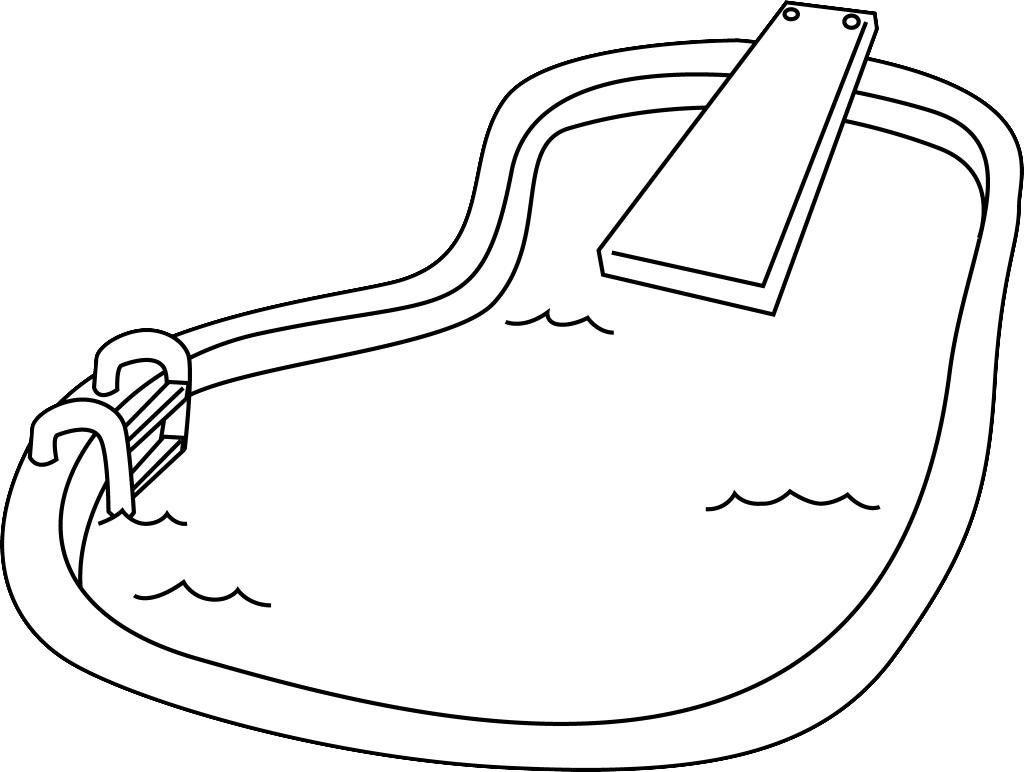
\includegraphics[width=0.4\textwidth]{figs/frontpage/smartpool.png}
\end{minipage}

\vspace{\fill}
\begin{minipage}[l]{\textwidth}
\begin{tabu} to \textwidth{lX[l]}
\textbf{Dato}           &\today\\
\textbf{Vejleder}		&Vejleder navn\\
\end{tabu}
\end{minipage}

\vspace{10pt}
\begin{minipage}[l]{\textwidth}
\tabulinesep=25pt
\begin{tabu} to \textwidth{X[l]X[l]X[l]}
 \makebox[\linewidth]{\hrulefill}\newline Joachim Dam Andersen     \newline 201370248/IKT  
&\makebox[\linewidth]{\hrulefill}\newline Lasse Priebe             \newline 201370248/IKT 
&\makebox[\linewidth]{\hrulefill}\newline Emil Nyborg              \newline 201370248/IKT\\
 \makebox[\linewidth]{\hrulefill}\newline Bjørn Nørgaard Sørensen  \newline 201370248/IKT  
&\makebox[\linewidth]{\hrulefill}\newline Alex Justesen Karlsen    \newline 201370248/IKT 
&\makebox[\linewidth]{\hrulefill}\newline Joachim Händel Noer Wind \newline 201370248/IKT
\end{tabu}
\end{minipage}\clearpage

%% Abstract
% Initial setup
\markboth{RESUMÉ/ABSTRACT}{RESUMÉ/ABSTRACT}
\abstractintoc
\abstractcol
\setlength{\abstitleskip}{-18pt}

% Abstract
\begin{abstract}
Rapporten omhandler et 3. semesterprojekt fra Ingeniørhøjskolen Aarhus Universitet udarbejdet med henblik på at producere et system, som kan fungere som dosering- og sorteringsanlæg til tabletter. Systemet er tiltænkt brug i ældreplejen, som en måde hvorpå fejlmedicinering kan undgås, og tabletsortering kan klares automatisk. Ydermere vil systemet kunne gøre personale og pårørende opmærksomme på, at brugeren ikke har afhentet sine tabletter, indenfor et givet tidsrum. Dette skal formidles ved hjælp af en Android applikation. Systemet og serveren samarbejder om at kontrollerer, hvad der dispenseres til den specifikke bruger og hvornår. Denne kommunikation er ikke fuldt ud implementeret endnu. Systemet var oprindeligt tiltænkt brug i private hjem, men undervejs i processen er idéen ændret idet at fokus flyttes fra private hjem til brug i plejesektoren. 
Produktet kan på nuværende tidspunkt dosere et bestemt antal tabletter af én enkelt type. Systemet har på nuværende tidspunkt allerede implementeret muligheden for at udvide med ekstra dispenserer, og er derfor velegnet til videreudvikling. 
Til systemet er der implementeret en fungerende brugergrænseflade, som er testet med en brugervenlighedsundersøgelse, der ved adspørgelse af 15 studerende har påpeget adskillige muligheder for forbedring.
Under systemudviklingen er den største arbejdsindsats lagt i undersøgelse af teknologier og mulige løsningsforslag.
\end{abstract}

\begin{abstracten}
The report covers a third semesterproject from the Aarhus University School of Engineering. The goal is to produce a system that can function as a dispensing and sorting machine for pills. The system is intended for use in eldercare, as a way of preventing medication errors and a way of sorting pills automaticly. Furthermore, the system will be able to notify staff and relatives if the elder has not picked up their pills, within a given timeperiod. The staff and relatives will be notified via an Android application. The system and a server operate together in order to control what is dispensed to whom and when. Though this communication is not fully implemented yet. The system was originally intended for use in private homes, but during the process, the idea evolved so that the focus was changed from home use to the healthcare sector.
The product can at this time dispense a certain number of pills which will have to be of a single type. The option of adding extra dispensers is already implemented, and is therefore suitable for further development.
The system also has a functioning interface implemented, which has been tested with a user-experience study in which 15 students participated. With the feedback made several things clear, and several of these are suitable for further work.
During the system development the largest effort was put into the study of technologies and potential solutions for the problem chosen.
\end{abstracten}\clearpage

%% Forord
\pagestyle{asereport}
\chapter{Forord}

% Forordet benyttes til at informere kort om visse ydre omstændigheder for projektet, såsom projekttype og hvor projektet er gennemført, historisk baggrund (andre arbejder, som har givet anledning til det aktuelle projekt) og hvor inspirationen og ideen er kommet fra, m.v.

Dette dokument er sammensat for at dokumentere arbejdet på 4. semesterprojektet for retningen IKT på ingeniørhøjskolen Århus.

Der vil i denne rapport være referencer til bilag og dokumentation, som det ikke ville være hensigtsmæssigt at medtage. Samtlige bilag m.m. vil være at finde på den vedlagt CD-rom. 

Source kode til projektet kan findes på CD'en. Link til vores github repo følger her: \newline \url{https://github.com/BjornNorgaard/DuckMaster3001}

\vspace{5mm}

\large{\textit{En stor tak til}}

\begin{displayquote}
    Lars Mortensen for god og brugbar vejledning.
\end{displayquote}

\begin{displayquote}
    Stjerne Apoteket for at lade gruppen komme på besøg og se deres sorteringsmaskine.
\end{displayquote}

\begin{displayquote}
    Sofie Fredslund for at lade os interviewe hende til projektet.
\end{displayquote}

\begin{displayquote}
   Underviserne på ASE, for hjælp og vejledning.
\end{displayquote}

\clearpage

%% ToC
\tableofcontents\clearpage

\mainmatter

%% Todo oversigt - SKAL UDKOMMENTERES FØR AFLEVERING
\listoftodos[Liste over gøremål]

%% Indledning
\chapter{Indledning}

Hello \cite{fysikbog} og sådan kan det jo gå.\clearpage

%% Projektformulering
\documentclass[a4paper,11pt,oneside]{memoir}
\input{utils/packages}
\input{utils/layout}
\input{utils/listings}
\input{utils/ordliste}

%% Forside variabler
\newcommand{\Kursus}{I4PRJ4 F16}
\newcommand{\Projektnavn}{SmartPool 2.0}
\newcommand{\Gruppe}{Gruppe 3}
\newcommand{\Projektdokument}{Projektrapport}

%% Litteratur
\nocite{*}
%\bibliographystyle{harvard}
\bibliography{utils/litteratur}

\begin{document}
\frontmatter

\input{utils/frontpage}\clearpage

%% Abstract
\input{docs/frontmatter/abstract}\clearpage

%% Forord
\pagestyle{asereport}
\input{docs/frontmatter/forord}\clearpage

%% ToC
\tableofcontents\clearpage

\mainmatter

%% Todo oversigt - SKAL UDKOMMENTERES FØR AFLEVERING
\listoftodos[Liste over gøremål]

%% Indledning
\input{docs/frontmatter/indledning}\clearpage

%% Projektformulering
\input{docs/projektformulering/main}\clearpage

%% Kravspecifikation
\input{docs/kravspecifikation/main}\clearpage

%% Systemarkitektur
\input{docs/systemarkitektur/main}\clearpage

%% Processbeskrivelse
\input{docs/processbeskrivelse/main}\clearpage

%% Design
\input{docs/design/main}\clearpage

%% Implementering
\input{docs/implementering/main}\clearpage

%% Integration
\input{docs/integration/main}\clearpage

%% Accepttest
\input{docs/accepttest/main}\clearpage

%% Appendix
\input{docs/appendix/main}\clearpage

\backmatter
%% Glossary
\setglossarystyle{list}
\printnoidxglossary[title=Ordliste]

% Bibliography
\clearpage
\printbibliography[title={Litteratur}]
\end{document}\clearpage

%% Kravspecifikation
\documentclass[a4paper,11pt,oneside]{memoir}
\input{utils/packages}
\input{utils/layout}
\input{utils/listings}
\input{utils/ordliste}

%% Forside variabler
\newcommand{\Kursus}{I4PRJ4 F16}
\newcommand{\Projektnavn}{SmartPool 2.0}
\newcommand{\Gruppe}{Gruppe 3}
\newcommand{\Projektdokument}{Projektrapport}

%% Litteratur
\nocite{*}
%\bibliographystyle{harvard}
\bibliography{utils/litteratur}

\begin{document}
\frontmatter

\input{utils/frontpage}\clearpage

%% Abstract
\input{docs/frontmatter/abstract}\clearpage

%% Forord
\pagestyle{asereport}
\input{docs/frontmatter/forord}\clearpage

%% ToC
\tableofcontents\clearpage

\mainmatter

%% Todo oversigt - SKAL UDKOMMENTERES FØR AFLEVERING
\listoftodos[Liste over gøremål]

%% Indledning
\input{docs/frontmatter/indledning}\clearpage

%% Projektformulering
\input{docs/projektformulering/main}\clearpage

%% Kravspecifikation
\input{docs/kravspecifikation/main}\clearpage

%% Systemarkitektur
\input{docs/systemarkitektur/main}\clearpage

%% Processbeskrivelse
\input{docs/processbeskrivelse/main}\clearpage

%% Design
\input{docs/design/main}\clearpage

%% Implementering
\input{docs/implementering/main}\clearpage

%% Integration
\input{docs/integration/main}\clearpage

%% Accepttest
\input{docs/accepttest/main}\clearpage

%% Appendix
\input{docs/appendix/main}\clearpage

\backmatter
%% Glossary
\setglossarystyle{list}
\printnoidxglossary[title=Ordliste]

% Bibliography
\clearpage
\printbibliography[title={Litteratur}]
\end{document}\clearpage

%% Systemarkitektur
\documentclass[a4paper,11pt,oneside]{memoir}
\input{utils/packages}
\input{utils/layout}
\input{utils/listings}
\input{utils/ordliste}

%% Forside variabler
\newcommand{\Kursus}{I4PRJ4 F16}
\newcommand{\Projektnavn}{SmartPool 2.0}
\newcommand{\Gruppe}{Gruppe 3}
\newcommand{\Projektdokument}{Projektrapport}

%% Litteratur
\nocite{*}
%\bibliographystyle{harvard}
\bibliography{utils/litteratur}

\begin{document}
\frontmatter

\input{utils/frontpage}\clearpage

%% Abstract
\input{docs/frontmatter/abstract}\clearpage

%% Forord
\pagestyle{asereport}
\input{docs/frontmatter/forord}\clearpage

%% ToC
\tableofcontents\clearpage

\mainmatter

%% Todo oversigt - SKAL UDKOMMENTERES FØR AFLEVERING
\listoftodos[Liste over gøremål]

%% Indledning
\input{docs/frontmatter/indledning}\clearpage

%% Projektformulering
\input{docs/projektformulering/main}\clearpage

%% Kravspecifikation
\input{docs/kravspecifikation/main}\clearpage

%% Systemarkitektur
\input{docs/systemarkitektur/main}\clearpage

%% Processbeskrivelse
\input{docs/processbeskrivelse/main}\clearpage

%% Design
\input{docs/design/main}\clearpage

%% Implementering
\input{docs/implementering/main}\clearpage

%% Integration
\input{docs/integration/main}\clearpage

%% Accepttest
\input{docs/accepttest/main}\clearpage

%% Appendix
\input{docs/appendix/main}\clearpage

\backmatter
%% Glossary
\setglossarystyle{list}
\printnoidxglossary[title=Ordliste]

% Bibliography
\clearpage
\printbibliography[title={Litteratur}]
\end{document}\clearpage

%% Processbeskrivelse
\documentclass[a4paper,11pt,oneside]{memoir}
\input{utils/packages}
\input{utils/layout}
\input{utils/listings}
\input{utils/ordliste}

%% Forside variabler
\newcommand{\Kursus}{I4PRJ4 F16}
\newcommand{\Projektnavn}{SmartPool 2.0}
\newcommand{\Gruppe}{Gruppe 3}
\newcommand{\Projektdokument}{Projektrapport}

%% Litteratur
\nocite{*}
%\bibliographystyle{harvard}
\bibliography{utils/litteratur}

\begin{document}
\frontmatter

\input{utils/frontpage}\clearpage

%% Abstract
\input{docs/frontmatter/abstract}\clearpage

%% Forord
\pagestyle{asereport}
\input{docs/frontmatter/forord}\clearpage

%% ToC
\tableofcontents\clearpage

\mainmatter

%% Todo oversigt - SKAL UDKOMMENTERES FØR AFLEVERING
\listoftodos[Liste over gøremål]

%% Indledning
\input{docs/frontmatter/indledning}\clearpage

%% Projektformulering
\input{docs/projektformulering/main}\clearpage

%% Kravspecifikation
\input{docs/kravspecifikation/main}\clearpage

%% Systemarkitektur
\input{docs/systemarkitektur/main}\clearpage

%% Processbeskrivelse
\input{docs/processbeskrivelse/main}\clearpage

%% Design
\input{docs/design/main}\clearpage

%% Implementering
\input{docs/implementering/main}\clearpage

%% Integration
\input{docs/integration/main}\clearpage

%% Accepttest
\input{docs/accepttest/main}\clearpage

%% Appendix
\input{docs/appendix/main}\clearpage

\backmatter
%% Glossary
\setglossarystyle{list}
\printnoidxglossary[title=Ordliste]

% Bibliography
\clearpage
\printbibliography[title={Litteratur}]
\end{document}\clearpage

%% Design
\documentclass[a4paper,11pt,oneside]{memoir}
\input{utils/packages}
\input{utils/layout}
\input{utils/listings}
\input{utils/ordliste}

%% Forside variabler
\newcommand{\Kursus}{I4PRJ4 F16}
\newcommand{\Projektnavn}{SmartPool 2.0}
\newcommand{\Gruppe}{Gruppe 3}
\newcommand{\Projektdokument}{Projektrapport}

%% Litteratur
\nocite{*}
%\bibliographystyle{harvard}
\bibliography{utils/litteratur}

\begin{document}
\frontmatter

\input{utils/frontpage}\clearpage

%% Abstract
\input{docs/frontmatter/abstract}\clearpage

%% Forord
\pagestyle{asereport}
\input{docs/frontmatter/forord}\clearpage

%% ToC
\tableofcontents\clearpage

\mainmatter

%% Todo oversigt - SKAL UDKOMMENTERES FØR AFLEVERING
\listoftodos[Liste over gøremål]

%% Indledning
\input{docs/frontmatter/indledning}\clearpage

%% Projektformulering
\input{docs/projektformulering/main}\clearpage

%% Kravspecifikation
\input{docs/kravspecifikation/main}\clearpage

%% Systemarkitektur
\input{docs/systemarkitektur/main}\clearpage

%% Processbeskrivelse
\input{docs/processbeskrivelse/main}\clearpage

%% Design
\input{docs/design/main}\clearpage

%% Implementering
\input{docs/implementering/main}\clearpage

%% Integration
\input{docs/integration/main}\clearpage

%% Accepttest
\input{docs/accepttest/main}\clearpage

%% Appendix
\input{docs/appendix/main}\clearpage

\backmatter
%% Glossary
\setglossarystyle{list}
\printnoidxglossary[title=Ordliste]

% Bibliography
\clearpage
\printbibliography[title={Litteratur}]
\end{document}\clearpage

%% Implementering
\documentclass[a4paper,11pt,oneside]{memoir}
\input{utils/packages}
\input{utils/layout}
\input{utils/listings}
\input{utils/ordliste}

%% Forside variabler
\newcommand{\Kursus}{I4PRJ4 F16}
\newcommand{\Projektnavn}{SmartPool 2.0}
\newcommand{\Gruppe}{Gruppe 3}
\newcommand{\Projektdokument}{Projektrapport}

%% Litteratur
\nocite{*}
%\bibliographystyle{harvard}
\bibliography{utils/litteratur}

\begin{document}
\frontmatter

\input{utils/frontpage}\clearpage

%% Abstract
\input{docs/frontmatter/abstract}\clearpage

%% Forord
\pagestyle{asereport}
\input{docs/frontmatter/forord}\clearpage

%% ToC
\tableofcontents\clearpage

\mainmatter

%% Todo oversigt - SKAL UDKOMMENTERES FØR AFLEVERING
\listoftodos[Liste over gøremål]

%% Indledning
\input{docs/frontmatter/indledning}\clearpage

%% Projektformulering
\input{docs/projektformulering/main}\clearpage

%% Kravspecifikation
\input{docs/kravspecifikation/main}\clearpage

%% Systemarkitektur
\input{docs/systemarkitektur/main}\clearpage

%% Processbeskrivelse
\input{docs/processbeskrivelse/main}\clearpage

%% Design
\input{docs/design/main}\clearpage

%% Implementering
\input{docs/implementering/main}\clearpage

%% Integration
\input{docs/integration/main}\clearpage

%% Accepttest
\input{docs/accepttest/main}\clearpage

%% Appendix
\input{docs/appendix/main}\clearpage

\backmatter
%% Glossary
\setglossarystyle{list}
\printnoidxglossary[title=Ordliste]

% Bibliography
\clearpage
\printbibliography[title={Litteratur}]
\end{document}\clearpage

%% Integration
\documentclass[a4paper,11pt,oneside]{memoir}
\input{utils/packages}
\input{utils/layout}
\input{utils/listings}
\input{utils/ordliste}

%% Forside variabler
\newcommand{\Kursus}{I4PRJ4 F16}
\newcommand{\Projektnavn}{SmartPool 2.0}
\newcommand{\Gruppe}{Gruppe 3}
\newcommand{\Projektdokument}{Projektrapport}

%% Litteratur
\nocite{*}
%\bibliographystyle{harvard}
\bibliography{utils/litteratur}

\begin{document}
\frontmatter

\input{utils/frontpage}\clearpage

%% Abstract
\input{docs/frontmatter/abstract}\clearpage

%% Forord
\pagestyle{asereport}
\input{docs/frontmatter/forord}\clearpage

%% ToC
\tableofcontents\clearpage

\mainmatter

%% Todo oversigt - SKAL UDKOMMENTERES FØR AFLEVERING
\listoftodos[Liste over gøremål]

%% Indledning
\input{docs/frontmatter/indledning}\clearpage

%% Projektformulering
\input{docs/projektformulering/main}\clearpage

%% Kravspecifikation
\input{docs/kravspecifikation/main}\clearpage

%% Systemarkitektur
\input{docs/systemarkitektur/main}\clearpage

%% Processbeskrivelse
\input{docs/processbeskrivelse/main}\clearpage

%% Design
\input{docs/design/main}\clearpage

%% Implementering
\input{docs/implementering/main}\clearpage

%% Integration
\input{docs/integration/main}\clearpage

%% Accepttest
\input{docs/accepttest/main}\clearpage

%% Appendix
\input{docs/appendix/main}\clearpage

\backmatter
%% Glossary
\setglossarystyle{list}
\printnoidxglossary[title=Ordliste]

% Bibliography
\clearpage
\printbibliography[title={Litteratur}]
\end{document}\clearpage

%% Accepttest
\documentclass[a4paper,11pt,oneside]{memoir}
\input{utils/packages}
\input{utils/layout}
\input{utils/listings}
\input{utils/ordliste}

%% Forside variabler
\newcommand{\Kursus}{I4PRJ4 F16}
\newcommand{\Projektnavn}{SmartPool 2.0}
\newcommand{\Gruppe}{Gruppe 3}
\newcommand{\Projektdokument}{Projektrapport}

%% Litteratur
\nocite{*}
%\bibliographystyle{harvard}
\bibliography{utils/litteratur}

\begin{document}
\frontmatter

\input{utils/frontpage}\clearpage

%% Abstract
\input{docs/frontmatter/abstract}\clearpage

%% Forord
\pagestyle{asereport}
\input{docs/frontmatter/forord}\clearpage

%% ToC
\tableofcontents\clearpage

\mainmatter

%% Todo oversigt - SKAL UDKOMMENTERES FØR AFLEVERING
\listoftodos[Liste over gøremål]

%% Indledning
\input{docs/frontmatter/indledning}\clearpage

%% Projektformulering
\input{docs/projektformulering/main}\clearpage

%% Kravspecifikation
\input{docs/kravspecifikation/main}\clearpage

%% Systemarkitektur
\input{docs/systemarkitektur/main}\clearpage

%% Processbeskrivelse
\input{docs/processbeskrivelse/main}\clearpage

%% Design
\input{docs/design/main}\clearpage

%% Implementering
\input{docs/implementering/main}\clearpage

%% Integration
\input{docs/integration/main}\clearpage

%% Accepttest
\input{docs/accepttest/main}\clearpage

%% Appendix
\input{docs/appendix/main}\clearpage

\backmatter
%% Glossary
\setglossarystyle{list}
\printnoidxglossary[title=Ordliste]

% Bibliography
\clearpage
\printbibliography[title={Litteratur}]
\end{document}\clearpage

%% Appendix
\documentclass[a4paper,11pt,oneside]{memoir}
\input{utils/packages}
\input{utils/layout}
\input{utils/listings}
\input{utils/ordliste}

%% Forside variabler
\newcommand{\Kursus}{I4PRJ4 F16}
\newcommand{\Projektnavn}{SmartPool 2.0}
\newcommand{\Gruppe}{Gruppe 3}
\newcommand{\Projektdokument}{Projektrapport}

%% Litteratur
\nocite{*}
%\bibliographystyle{harvard}
\bibliography{utils/litteratur}

\begin{document}
\frontmatter

\input{utils/frontpage}\clearpage

%% Abstract
\input{docs/frontmatter/abstract}\clearpage

%% Forord
\pagestyle{asereport}
\input{docs/frontmatter/forord}\clearpage

%% ToC
\tableofcontents\clearpage

\mainmatter

%% Todo oversigt - SKAL UDKOMMENTERES FØR AFLEVERING
\listoftodos[Liste over gøremål]

%% Indledning
\input{docs/frontmatter/indledning}\clearpage

%% Projektformulering
\input{docs/projektformulering/main}\clearpage

%% Kravspecifikation
\input{docs/kravspecifikation/main}\clearpage

%% Systemarkitektur
\input{docs/systemarkitektur/main}\clearpage

%% Processbeskrivelse
\input{docs/processbeskrivelse/main}\clearpage

%% Design
\input{docs/design/main}\clearpage

%% Implementering
\input{docs/implementering/main}\clearpage

%% Integration
\input{docs/integration/main}\clearpage

%% Accepttest
\input{docs/accepttest/main}\clearpage

%% Appendix
\input{docs/appendix/main}\clearpage

\backmatter
%% Glossary
\setglossarystyle{list}
\printnoidxglossary[title=Ordliste]

% Bibliography
\clearpage
\printbibliography[title={Litteratur}]
\end{document}\clearpage

\backmatter
%% Glossary
\setglossarystyle{list}
\printnoidxglossary[title=Ordliste]

% Bibliography
\clearpage
\printbibliography[title={Litteratur}]
\end{document}\clearpage

%% Appendix
\documentclass[a4paper,11pt,oneside]{memoir}
%!TEX root = main.tex
% Encoding
%\usepackage[utf8]{inputenc} % pdfLatex
\usepackage[T1]{fontenc}
\usepackage[danish]{babel}
\renewcommand{\danishhyphenmins}{22}
\usepackage[utf8]{inputenc} % æ ø å

% Date
\usepackage[ddmmyyyy]{datetime}
\renewcommand{\dateseparator}{.}

% Fonts
\usepackage{fourier}
\usepackage[scaled=0.8]{beramono}

% Math
\usepackage{amsmath,amssymb}
\usepackage{bm}
\usepackage{amsthm}
\usepackage{mathtools}

% Graphics
\usepackage[usenames,dvipsnames,table]{xcolor}
\usepackage{graphicx}
\usepackage{float}
%\usepackage[section]{placeins}
\usepackage{tikz}
\usepackage[pages=some]{background}
\usepackage{wrapfig}

% Listings & Tables
\usepackage{listings}
%\usepackage{pythontex}
\usepackage{enumitem}
\usepackage{tabu}
\usepackage{longtable}
\usepackage{multirow}
\usepackage{makecell}


% References & Quotes
%\usepackage[danish]{varioref}				% Muliggoer bl.a. krydshenvisninger med sidetal (\vref)
%\usepackage{nat}							% Udvidelse med naturvidenskabelige citationsmodeller
\usepackage[danish=guillemets]{csquotes}
\usepackage[hidelinks]{hyperref}
\hypersetup{
    pdfstartview={FitH},
    pdftitle={Smart Pool 2.0},
    pdfsubject={Projektrapport},
    pdfauthor={I4PRJ4GRP3}
}
\usepackage[all]{hypcap}

% Etc
\usepackage[
	%backend=biber,
	backend=bibtex,
	style=ieee,
	natbib=true,
	backref=false,
	backrefstyle=all+,
	hyperref=true
]{biblatex}
\usepackage{pdflscape}
\usepackage[nomain,toc,xindy,acronym,nonumberlist,noredefwarn]{glossaries}
\usepackage[xindy]{imakeidx}
\usepackage{float}
\makeindex

% Dummy
\usepackage{lipsum}
%!TEX root = main.tex
% Page setup
\setulmarginsandblock{35mm}{25mm}{*}
\setlrmarginsandblock{20mm}{20mm}{*}
\setheadfoot{4\onelineskip}{2\onelineskip}
\setheaderspaces{*}{5mm}{*}
\checkandfixthelayout

% Pagestyle
\makepagestyle{asereport}
	\makeevenhead{asereport}{}{}{}
	\makeoddhead{asereport}{
\includegraphics{figs/frontpage/aseaulogo.pdf}}{}{\small\rightmark{} | \textbf{\thepage{}\vspace{7pt}}}
	\makeevenfoot{asereport}{}{}{}
	\makeoddfoot{asereport}{}{}{}

\makepsmarks{asereport}{
	\createmark{chapter}{both}{shownumber}{}{. \ }
	\createmark{section}{both}{shownumber}{}{. \ }
	\createmark{subsection}{both}{shownumber}{}{. \ }
	\createplainmark{toc}{both}{\contentsname}
	\createplainmark{lof}{both}{\listfigurename}
	\createplainmark{lot}{both}{\listtablename}
	\createplainmark{bib}{both}{\bibname}
	\createplainmark{index}{both}{\indexname}
	\createplainmark{glossary}{both}{\glossaryname}
}

\aliaspagestyle{part}{asereport}
\aliaspagestyle{chapter}{asereport}
\chapterstyle{tandh}

% Modification to certain spacing
\setlength{\parskip}{8pt}
\setlength{\parindent}{0pt}
\setlength{\abovecaptionskip}{7pt}
\setlength{\belowcaptionskip}{-10pt}
\OnehalfSpacing

% Tabu
%\taburowcolors[1]2{white .. light-gray}
\tabulinesep=4pt

% Itemize/enumerate
\setlist{
    before=\vspace{-3pt}, 
    after=\vspace{-3pt},
    itemsep=0pt,
    leftmargin=25pt,
    labelsep=10pt,
    topsep=0pt,
}

% Kommandoer til UC - fixer spacing
% Aktører
\newcommand{\fua}[1]{
	\begin{minipage}[t]{\linewidth}
		\setlist{
		    leftmargin=22pt,
		    itemsep=0pt,
		    topsep=0pt,
		    parsep=3pt
		}
	\begin{itemize}[before={\vspace{-6pt}}, after={\vspace{6pt}}]
	#1
	\end{itemize}
	\end{minipage}
}

% Hovedforløb
\newcommand{\fu}[1]{
\begin{minipage}[t]{\linewidth}
\setlist{
    leftmargin=22pt,
    itemsep=0pt,
    topsep=0pt,
    parsep=3pt
}
\raggedright
\begin{enumerate}[before={\vspace{-5pt}},after={\vspace{6pt}}]
#1
\end{enumerate}
\end{minipage}}

% Extensions
\newcommand{\fuex}[2]{
\begin{minipage}[t]{\linewidth}
\vspace{-6pt}
\raggedright
\textit{#1}
\begin{enumerate}[leftmargin=22pt,itemsep=0pt,parsep=3pt,before={\vspace{-8pt}}, after={\vspace{20pt}},topsep=8pt]
#2
\end{enumerate}
\end{minipage}
}

% Extensions - Sidste entry
\newcommand{\fuexl}[2]{
\begin{minipage}[t]{\linewidth}
\vspace{-6pt}
\raggedright
\textit{#1}
\begin{enumerate}[leftmargin=22pt,itemsep=0pt,parsep=3pt,before={\vspace{-8pt}}, after={\vspace{3pt}},topsep=8pt]
#2
\end{enumerate}
\end{minipage}}

% Versionshistorik
\newcommand{\verhistitem}[2]{
\begin{minipage}[t]{\linewidth}
\vspace{-6pt}
\raggedright
#1
\begin{itemize}[leftmargin=22pt,itemsep=0pt,parsep=0pt,before={\vspace{-10pt}},after={\vspace{3pt}},topsep=8pt]
#2
\end{itemize}
\end{minipage}}

\newcommand{\tverb}[1]{{\texttt{#1}}}

\newcommand{\cond}[1]{
\begin{itemize}[label=,noitemsep,topsep=0pt,after={\vspace*{-\baselineskip}}]
#1
\end{itemize}}

% Etc
\definecolor{light-gray}{gray}{0.8}
\definecolor{pantone}{RGB}{0,61,133}

\setfloatlocations{figure}{H}
\setfloatlocations{table}{H}

\numberwithin{equation}{chapter}
\numberwithin{figure}{chapter}
\setcounter{secnumdepth}{3}
\setcounter{tocdepth}{2}
\maxsecnumdepth{subsection}

\renewcommand*{\cftdotsep}{1}
\setpnumwidth{2em}
\setrmarg{2em}

\setverbatimfont{\ttfamily}

%\renewcommand\cftchaptername {\chaptername~}
%\renewcommand\cftappendixname {\appendixname~}
\addto\captionsdanish{
    \renewcommand\contentsname{Indholdsfortegnelse}
    \renewcommand\appendixname{Appendiks}
}
\renewcommand\appendixpagename{Appendiks}
\renewcommand\appendixtocname{Appendiks}
\newsubfloat{figure}

% Abstract
\newenvironment{abstracten}
{\renewcommand{\abstractname}{Abstract}\abstract}
{\endabstract}
\renewcommand{\abstractnamefont}{\normalfont\Large\bfseries}
%!TEX root = main.tex
% Listings
\AtBeginDocument{%
  \counterwithin*{lstlisting}{section}
  \counterwithin*{lstlisting}{subsection}
  \counterwithin*{lstlisting}{subsubsection}
  \renewcommand{\thelstlisting}{%
    \ifnum\value{subsection}=0
      \thesection.\arabic{lstlisting}%
    \else
      \ifnum\value{subsubsection}=0
        \thesubsection.\arabic{lstlisting}%
      \else
        \thesubsubsection.\arabic{lstlisting}%
      \fi
    \fi
  }
}

% Loading languages
\lstloadlanguages{C, C++}

% Listing setup
\lstdefinestyle{all}{
    basicstyle    = \ttfamily\SingleSpacing\scriptsize,
    numbers       = left, 
    numberstyle   = \ttfamily\tiny,
    breaklines    = true,
    commentstyle=\color{green},
    %backgroundcolor = \color{red},
    numbersep     = 20pt,
    xleftmargin   = \parindent,
    captionpos    = b,
    keywordstyle  = [1]\color{Blue}\bfseries,
    commentstyle  = \itshape\color{Green},
    tabsize       = 3
}

\lstset{
    style = all
} 
%!TEX root = main.tex
\makenoidxglossaries
\newglossaryentry{gui}{
    name={GUI}, 
    description={Graphical User Interface er en brugergrænseflade. Brugerens måde at tilgå systemet på}}

\newglossaryentry{psoc}{
    name={PSoC}, 
    description={PSoC (Programmable System-on-Chip) er et microcontroller system produceret af Cypress Semiconductor}}

\newglossaryentry{moscow}{
    name={MoSCoW}, 
    description={MoSCoW er en metode til at prioritere krav til ens system}}

\newglossaryentry{furps}{
    name={FURPS}, 
    description={FURPS er en metode til kategorisering af systemets ikke-funktionelle krav}}

\newglossaryentry{BDD}{
    name={BDD}, 
    description={BDD (Block Definition Diagram) er et diagram, som beskriver et system ved at opdele det op i mindre blokke}}

\newglossaryentry{IBD}{
    name={IBD}, 
    description={IBD (Internal Block Diagram) er et diagram, som viser forbindelserne mellem blokkene, som kan findes i et BDD}}

\newglossaryentry{pilleskuffe}{
    name={Pilleskuffe},
    description={Skuffen under dispenseren, hvor i den nederste pille ligger i. Skuffen tømmes ved at elektromagneten trækker skuffen til sig.}}

\newglossaryentry{pilledispenser}{
    name={Pilledispenser},
    description={Det rør som pillerne bliver opbevaret i.}}

\newglossaryentry{elektromagneten}{
    name={Elektromagneten},
    description={Elektromagneten er en spole der sendes strøm igennem. Når der er strøm på spolen dannes et magnetfelt. Der vil ofte være tale om det samme hvad enten der står spole eller elektromagnet.}}

%% Forside variabler
\newcommand{\Kursus}{I4PRJ4 F16}
\newcommand{\Projektnavn}{SmartPool 2.0}
\newcommand{\Gruppe}{Gruppe 3}
\newcommand{\Projektdokument}{Projektrapport}

%% Litteratur
\nocite{*}
%\bibliographystyle{harvard}
\bibliography{utils/litteratur}

\begin{document}
\frontmatter

%!TEX root = main.tex
\pagestyle{titlingpage}
\backgroundsetup{
	scale=1,
	angle=0,
	opacity=1,
	contents={
		\begin{tikzpicture}[remember picture,overlay]
		\path [fill=pantone] (-0.5\paperwidth,0.36\paperheight) rectangle (0.5\paperwidth,0.47\paperheight);  
		\path [fill=pantone] (-0.5\paperwidth,-0.47\paperheight) rectangle (0.5\paperwidth,-0.43\paperheight);  
		\end{tikzpicture}}}
\BgThispage
\vspace*{-25mm}
\begin{minipage}[l]{\textwidth}
	
\includegraphics[width=0.75\textwidth]{figs/frontpage/aseaulogohvid.pdf}
\end{minipage}

\vspace{35pt}
\begin{minipage}[l]{\textwidth}
\tabulinesep=10pt
\begin{tabu} to \textwidth{X[l]}
	{\small\MakeUppercase\Kursus}\\
	{\HUGE\bfseries\MakeUppercase\Projektnavn}\\
	{\Large\Gruppe}\\
	{\itshape\Projektdokument}
\end{tabu}
\end{minipage}

\vspace{5pt}
\begin{minipage}[l]{\textwidth}
    \centering
	\vspace*{0cm}\hspace*{8cm}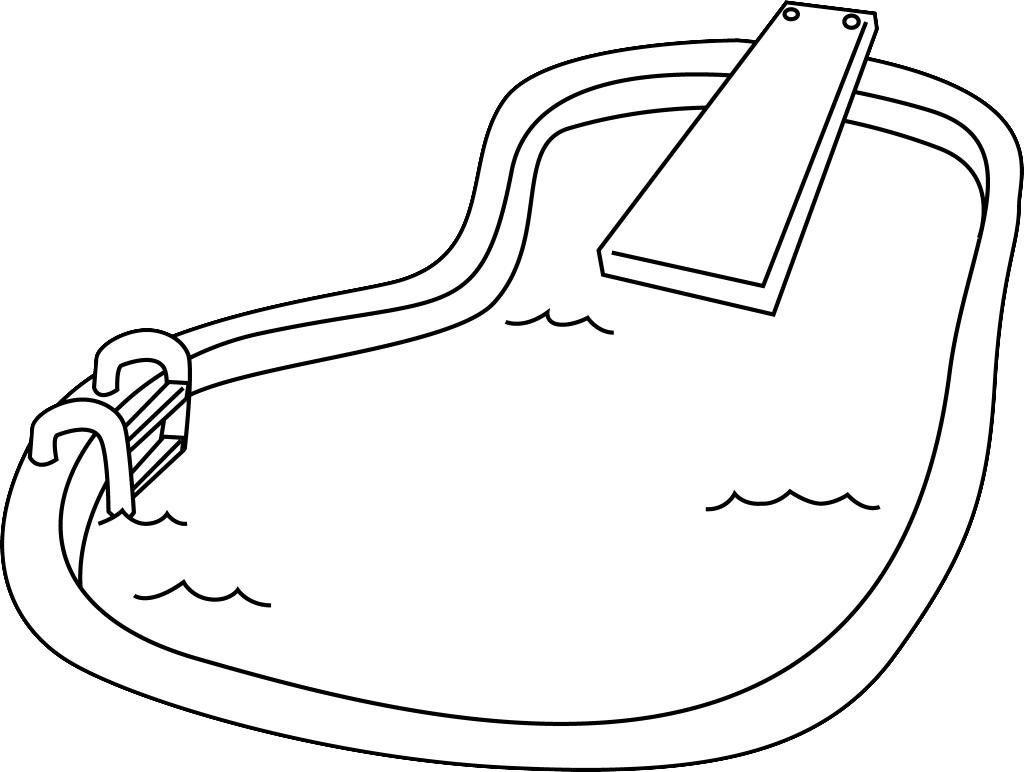
\includegraphics[width=0.4\textwidth]{figs/frontpage/smartpool.png}
\end{minipage}

\vspace{\fill}
\begin{minipage}[l]{\textwidth}
\begin{tabu} to \textwidth{lX[l]}
\textbf{Dato}           &\today\\
\textbf{Vejleder}		&Vejleder navn\\
\end{tabu}
\end{minipage}

\vspace{10pt}
\begin{minipage}[l]{\textwidth}
\tabulinesep=25pt
\begin{tabu} to \textwidth{X[l]X[l]X[l]}
 \makebox[\linewidth]{\hrulefill}\newline Joachim Dam Andersen     \newline 201370248/IKT  
&\makebox[\linewidth]{\hrulefill}\newline Lasse Priebe             \newline 201370248/IKT 
&\makebox[\linewidth]{\hrulefill}\newline Emil Nyborg              \newline 201370248/IKT\\
 \makebox[\linewidth]{\hrulefill}\newline Bjørn Nørgaard Sørensen  \newline 201370248/IKT  
&\makebox[\linewidth]{\hrulefill}\newline Alex Justesen Karlsen    \newline 201370248/IKT 
&\makebox[\linewidth]{\hrulefill}\newline Joachim Händel Noer Wind \newline 201370248/IKT
\end{tabu}
\end{minipage}\clearpage

%% Abstract
% Initial setup
\markboth{RESUMÉ/ABSTRACT}{RESUMÉ/ABSTRACT}
\abstractintoc
\abstractcol
\setlength{\abstitleskip}{-18pt}

% Abstract
\begin{abstract}
Rapporten omhandler et 3. semesterprojekt fra Ingeniørhøjskolen Aarhus Universitet udarbejdet med henblik på at producere et system, som kan fungere som dosering- og sorteringsanlæg til tabletter. Systemet er tiltænkt brug i ældreplejen, som en måde hvorpå fejlmedicinering kan undgås, og tabletsortering kan klares automatisk. Ydermere vil systemet kunne gøre personale og pårørende opmærksomme på, at brugeren ikke har afhentet sine tabletter, indenfor et givet tidsrum. Dette skal formidles ved hjælp af en Android applikation. Systemet og serveren samarbejder om at kontrollerer, hvad der dispenseres til den specifikke bruger og hvornår. Denne kommunikation er ikke fuldt ud implementeret endnu. Systemet var oprindeligt tiltænkt brug i private hjem, men undervejs i processen er idéen ændret idet at fokus flyttes fra private hjem til brug i plejesektoren. 
Produktet kan på nuværende tidspunkt dosere et bestemt antal tabletter af én enkelt type. Systemet har på nuværende tidspunkt allerede implementeret muligheden for at udvide med ekstra dispenserer, og er derfor velegnet til videreudvikling. 
Til systemet er der implementeret en fungerende brugergrænseflade, som er testet med en brugervenlighedsundersøgelse, der ved adspørgelse af 15 studerende har påpeget adskillige muligheder for forbedring.
Under systemudviklingen er den største arbejdsindsats lagt i undersøgelse af teknologier og mulige løsningsforslag.
\end{abstract}

\begin{abstracten}
The report covers a third semesterproject from the Aarhus University School of Engineering. The goal is to produce a system that can function as a dispensing and sorting machine for pills. The system is intended for use in eldercare, as a way of preventing medication errors and a way of sorting pills automaticly. Furthermore, the system will be able to notify staff and relatives if the elder has not picked up their pills, within a given timeperiod. The staff and relatives will be notified via an Android application. The system and a server operate together in order to control what is dispensed to whom and when. Though this communication is not fully implemented yet. The system was originally intended for use in private homes, but during the process, the idea evolved so that the focus was changed from home use to the healthcare sector.
The product can at this time dispense a certain number of pills which will have to be of a single type. The option of adding extra dispensers is already implemented, and is therefore suitable for further development.
The system also has a functioning interface implemented, which has been tested with a user-experience study in which 15 students participated. With the feedback made several things clear, and several of these are suitable for further work.
During the system development the largest effort was put into the study of technologies and potential solutions for the problem chosen.
\end{abstracten}\clearpage

%% Forord
\pagestyle{asereport}
\chapter{Forord}

% Forordet benyttes til at informere kort om visse ydre omstændigheder for projektet, såsom projekttype og hvor projektet er gennemført, historisk baggrund (andre arbejder, som har givet anledning til det aktuelle projekt) og hvor inspirationen og ideen er kommet fra, m.v.

Dette dokument er sammensat for at dokumentere arbejdet på 4. semesterprojektet for retningen IKT på ingeniørhøjskolen Århus.

Der vil i denne rapport være referencer til bilag og dokumentation, som det ikke ville være hensigtsmæssigt at medtage. Samtlige bilag m.m. vil være at finde på den vedlagt CD-rom. 

Source kode til projektet kan findes på CD'en. Link til vores github repo følger her: \newline \url{https://github.com/BjornNorgaard/DuckMaster3001}

\vspace{5mm}

\large{\textit{En stor tak til}}

\begin{displayquote}
    Lars Mortensen for god og brugbar vejledning.
\end{displayquote}

\begin{displayquote}
    Stjerne Apoteket for at lade gruppen komme på besøg og se deres sorteringsmaskine.
\end{displayquote}

\begin{displayquote}
    Sofie Fredslund for at lade os interviewe hende til projektet.
\end{displayquote}

\begin{displayquote}
   Underviserne på ASE, for hjælp og vejledning.
\end{displayquote}

\clearpage

%% ToC
\tableofcontents\clearpage

\mainmatter

%% Todo oversigt - SKAL UDKOMMENTERES FØR AFLEVERING
\listoftodos[Liste over gøremål]

%% Indledning
\chapter{Indledning}

Hello \cite{fysikbog} og sådan kan det jo gå.\clearpage

%% Projektformulering
\documentclass[a4paper,11pt,oneside]{memoir}
\input{utils/packages}
\input{utils/layout}
\input{utils/listings}
\input{utils/ordliste}

%% Forside variabler
\newcommand{\Kursus}{I4PRJ4 F16}
\newcommand{\Projektnavn}{SmartPool 2.0}
\newcommand{\Gruppe}{Gruppe 3}
\newcommand{\Projektdokument}{Projektrapport}

%% Litteratur
\nocite{*}
%\bibliographystyle{harvard}
\bibliography{utils/litteratur}

\begin{document}
\frontmatter

\input{utils/frontpage}\clearpage

%% Abstract
\input{docs/frontmatter/abstract}\clearpage

%% Forord
\pagestyle{asereport}
\input{docs/frontmatter/forord}\clearpage

%% ToC
\tableofcontents\clearpage

\mainmatter

%% Todo oversigt - SKAL UDKOMMENTERES FØR AFLEVERING
\listoftodos[Liste over gøremål]

%% Indledning
\input{docs/frontmatter/indledning}\clearpage

%% Projektformulering
\input{docs/projektformulering/main}\clearpage

%% Kravspecifikation
\input{docs/kravspecifikation/main}\clearpage

%% Systemarkitektur
\input{docs/systemarkitektur/main}\clearpage

%% Processbeskrivelse
\input{docs/processbeskrivelse/main}\clearpage

%% Design
\input{docs/design/main}\clearpage

%% Implementering
\input{docs/implementering/main}\clearpage

%% Integration
\input{docs/integration/main}\clearpage

%% Accepttest
\input{docs/accepttest/main}\clearpage

%% Appendix
\input{docs/appendix/main}\clearpage

\backmatter
%% Glossary
\setglossarystyle{list}
\printnoidxglossary[title=Ordliste]

% Bibliography
\clearpage
\printbibliography[title={Litteratur}]
\end{document}\clearpage

%% Kravspecifikation
\documentclass[a4paper,11pt,oneside]{memoir}
\input{utils/packages}
\input{utils/layout}
\input{utils/listings}
\input{utils/ordliste}

%% Forside variabler
\newcommand{\Kursus}{I4PRJ4 F16}
\newcommand{\Projektnavn}{SmartPool 2.0}
\newcommand{\Gruppe}{Gruppe 3}
\newcommand{\Projektdokument}{Projektrapport}

%% Litteratur
\nocite{*}
%\bibliographystyle{harvard}
\bibliography{utils/litteratur}

\begin{document}
\frontmatter

\input{utils/frontpage}\clearpage

%% Abstract
\input{docs/frontmatter/abstract}\clearpage

%% Forord
\pagestyle{asereport}
\input{docs/frontmatter/forord}\clearpage

%% ToC
\tableofcontents\clearpage

\mainmatter

%% Todo oversigt - SKAL UDKOMMENTERES FØR AFLEVERING
\listoftodos[Liste over gøremål]

%% Indledning
\input{docs/frontmatter/indledning}\clearpage

%% Projektformulering
\input{docs/projektformulering/main}\clearpage

%% Kravspecifikation
\input{docs/kravspecifikation/main}\clearpage

%% Systemarkitektur
\input{docs/systemarkitektur/main}\clearpage

%% Processbeskrivelse
\input{docs/processbeskrivelse/main}\clearpage

%% Design
\input{docs/design/main}\clearpage

%% Implementering
\input{docs/implementering/main}\clearpage

%% Integration
\input{docs/integration/main}\clearpage

%% Accepttest
\input{docs/accepttest/main}\clearpage

%% Appendix
\input{docs/appendix/main}\clearpage

\backmatter
%% Glossary
\setglossarystyle{list}
\printnoidxglossary[title=Ordliste]

% Bibliography
\clearpage
\printbibliography[title={Litteratur}]
\end{document}\clearpage

%% Systemarkitektur
\documentclass[a4paper,11pt,oneside]{memoir}
\input{utils/packages}
\input{utils/layout}
\input{utils/listings}
\input{utils/ordliste}

%% Forside variabler
\newcommand{\Kursus}{I4PRJ4 F16}
\newcommand{\Projektnavn}{SmartPool 2.0}
\newcommand{\Gruppe}{Gruppe 3}
\newcommand{\Projektdokument}{Projektrapport}

%% Litteratur
\nocite{*}
%\bibliographystyle{harvard}
\bibliography{utils/litteratur}

\begin{document}
\frontmatter

\input{utils/frontpage}\clearpage

%% Abstract
\input{docs/frontmatter/abstract}\clearpage

%% Forord
\pagestyle{asereport}
\input{docs/frontmatter/forord}\clearpage

%% ToC
\tableofcontents\clearpage

\mainmatter

%% Todo oversigt - SKAL UDKOMMENTERES FØR AFLEVERING
\listoftodos[Liste over gøremål]

%% Indledning
\input{docs/frontmatter/indledning}\clearpage

%% Projektformulering
\input{docs/projektformulering/main}\clearpage

%% Kravspecifikation
\input{docs/kravspecifikation/main}\clearpage

%% Systemarkitektur
\input{docs/systemarkitektur/main}\clearpage

%% Processbeskrivelse
\input{docs/processbeskrivelse/main}\clearpage

%% Design
\input{docs/design/main}\clearpage

%% Implementering
\input{docs/implementering/main}\clearpage

%% Integration
\input{docs/integration/main}\clearpage

%% Accepttest
\input{docs/accepttest/main}\clearpage

%% Appendix
\input{docs/appendix/main}\clearpage

\backmatter
%% Glossary
\setglossarystyle{list}
\printnoidxglossary[title=Ordliste]

% Bibliography
\clearpage
\printbibliography[title={Litteratur}]
\end{document}\clearpage

%% Processbeskrivelse
\documentclass[a4paper,11pt,oneside]{memoir}
\input{utils/packages}
\input{utils/layout}
\input{utils/listings}
\input{utils/ordliste}

%% Forside variabler
\newcommand{\Kursus}{I4PRJ4 F16}
\newcommand{\Projektnavn}{SmartPool 2.0}
\newcommand{\Gruppe}{Gruppe 3}
\newcommand{\Projektdokument}{Projektrapport}

%% Litteratur
\nocite{*}
%\bibliographystyle{harvard}
\bibliography{utils/litteratur}

\begin{document}
\frontmatter

\input{utils/frontpage}\clearpage

%% Abstract
\input{docs/frontmatter/abstract}\clearpage

%% Forord
\pagestyle{asereport}
\input{docs/frontmatter/forord}\clearpage

%% ToC
\tableofcontents\clearpage

\mainmatter

%% Todo oversigt - SKAL UDKOMMENTERES FØR AFLEVERING
\listoftodos[Liste over gøremål]

%% Indledning
\input{docs/frontmatter/indledning}\clearpage

%% Projektformulering
\input{docs/projektformulering/main}\clearpage

%% Kravspecifikation
\input{docs/kravspecifikation/main}\clearpage

%% Systemarkitektur
\input{docs/systemarkitektur/main}\clearpage

%% Processbeskrivelse
\input{docs/processbeskrivelse/main}\clearpage

%% Design
\input{docs/design/main}\clearpage

%% Implementering
\input{docs/implementering/main}\clearpage

%% Integration
\input{docs/integration/main}\clearpage

%% Accepttest
\input{docs/accepttest/main}\clearpage

%% Appendix
\input{docs/appendix/main}\clearpage

\backmatter
%% Glossary
\setglossarystyle{list}
\printnoidxglossary[title=Ordliste]

% Bibliography
\clearpage
\printbibliography[title={Litteratur}]
\end{document}\clearpage

%% Design
\documentclass[a4paper,11pt,oneside]{memoir}
\input{utils/packages}
\input{utils/layout}
\input{utils/listings}
\input{utils/ordliste}

%% Forside variabler
\newcommand{\Kursus}{I4PRJ4 F16}
\newcommand{\Projektnavn}{SmartPool 2.0}
\newcommand{\Gruppe}{Gruppe 3}
\newcommand{\Projektdokument}{Projektrapport}

%% Litteratur
\nocite{*}
%\bibliographystyle{harvard}
\bibliography{utils/litteratur}

\begin{document}
\frontmatter

\input{utils/frontpage}\clearpage

%% Abstract
\input{docs/frontmatter/abstract}\clearpage

%% Forord
\pagestyle{asereport}
\input{docs/frontmatter/forord}\clearpage

%% ToC
\tableofcontents\clearpage

\mainmatter

%% Todo oversigt - SKAL UDKOMMENTERES FØR AFLEVERING
\listoftodos[Liste over gøremål]

%% Indledning
\input{docs/frontmatter/indledning}\clearpage

%% Projektformulering
\input{docs/projektformulering/main}\clearpage

%% Kravspecifikation
\input{docs/kravspecifikation/main}\clearpage

%% Systemarkitektur
\input{docs/systemarkitektur/main}\clearpage

%% Processbeskrivelse
\input{docs/processbeskrivelse/main}\clearpage

%% Design
\input{docs/design/main}\clearpage

%% Implementering
\input{docs/implementering/main}\clearpage

%% Integration
\input{docs/integration/main}\clearpage

%% Accepttest
\input{docs/accepttest/main}\clearpage

%% Appendix
\input{docs/appendix/main}\clearpage

\backmatter
%% Glossary
\setglossarystyle{list}
\printnoidxglossary[title=Ordliste]

% Bibliography
\clearpage
\printbibliography[title={Litteratur}]
\end{document}\clearpage

%% Implementering
\documentclass[a4paper,11pt,oneside]{memoir}
\input{utils/packages}
\input{utils/layout}
\input{utils/listings}
\input{utils/ordliste}

%% Forside variabler
\newcommand{\Kursus}{I4PRJ4 F16}
\newcommand{\Projektnavn}{SmartPool 2.0}
\newcommand{\Gruppe}{Gruppe 3}
\newcommand{\Projektdokument}{Projektrapport}

%% Litteratur
\nocite{*}
%\bibliographystyle{harvard}
\bibliography{utils/litteratur}

\begin{document}
\frontmatter

\input{utils/frontpage}\clearpage

%% Abstract
\input{docs/frontmatter/abstract}\clearpage

%% Forord
\pagestyle{asereport}
\input{docs/frontmatter/forord}\clearpage

%% ToC
\tableofcontents\clearpage

\mainmatter

%% Todo oversigt - SKAL UDKOMMENTERES FØR AFLEVERING
\listoftodos[Liste over gøremål]

%% Indledning
\input{docs/frontmatter/indledning}\clearpage

%% Projektformulering
\input{docs/projektformulering/main}\clearpage

%% Kravspecifikation
\input{docs/kravspecifikation/main}\clearpage

%% Systemarkitektur
\input{docs/systemarkitektur/main}\clearpage

%% Processbeskrivelse
\input{docs/processbeskrivelse/main}\clearpage

%% Design
\input{docs/design/main}\clearpage

%% Implementering
\input{docs/implementering/main}\clearpage

%% Integration
\input{docs/integration/main}\clearpage

%% Accepttest
\input{docs/accepttest/main}\clearpage

%% Appendix
\input{docs/appendix/main}\clearpage

\backmatter
%% Glossary
\setglossarystyle{list}
\printnoidxglossary[title=Ordliste]

% Bibliography
\clearpage
\printbibliography[title={Litteratur}]
\end{document}\clearpage

%% Integration
\documentclass[a4paper,11pt,oneside]{memoir}
\input{utils/packages}
\input{utils/layout}
\input{utils/listings}
\input{utils/ordliste}

%% Forside variabler
\newcommand{\Kursus}{I4PRJ4 F16}
\newcommand{\Projektnavn}{SmartPool 2.0}
\newcommand{\Gruppe}{Gruppe 3}
\newcommand{\Projektdokument}{Projektrapport}

%% Litteratur
\nocite{*}
%\bibliographystyle{harvard}
\bibliography{utils/litteratur}

\begin{document}
\frontmatter

\input{utils/frontpage}\clearpage

%% Abstract
\input{docs/frontmatter/abstract}\clearpage

%% Forord
\pagestyle{asereport}
\input{docs/frontmatter/forord}\clearpage

%% ToC
\tableofcontents\clearpage

\mainmatter

%% Todo oversigt - SKAL UDKOMMENTERES FØR AFLEVERING
\listoftodos[Liste over gøremål]

%% Indledning
\input{docs/frontmatter/indledning}\clearpage

%% Projektformulering
\input{docs/projektformulering/main}\clearpage

%% Kravspecifikation
\input{docs/kravspecifikation/main}\clearpage

%% Systemarkitektur
\input{docs/systemarkitektur/main}\clearpage

%% Processbeskrivelse
\input{docs/processbeskrivelse/main}\clearpage

%% Design
\input{docs/design/main}\clearpage

%% Implementering
\input{docs/implementering/main}\clearpage

%% Integration
\input{docs/integration/main}\clearpage

%% Accepttest
\input{docs/accepttest/main}\clearpage

%% Appendix
\input{docs/appendix/main}\clearpage

\backmatter
%% Glossary
\setglossarystyle{list}
\printnoidxglossary[title=Ordliste]

% Bibliography
\clearpage
\printbibliography[title={Litteratur}]
\end{document}\clearpage

%% Accepttest
\documentclass[a4paper,11pt,oneside]{memoir}
\input{utils/packages}
\input{utils/layout}
\input{utils/listings}
\input{utils/ordliste}

%% Forside variabler
\newcommand{\Kursus}{I4PRJ4 F16}
\newcommand{\Projektnavn}{SmartPool 2.0}
\newcommand{\Gruppe}{Gruppe 3}
\newcommand{\Projektdokument}{Projektrapport}

%% Litteratur
\nocite{*}
%\bibliographystyle{harvard}
\bibliography{utils/litteratur}

\begin{document}
\frontmatter

\input{utils/frontpage}\clearpage

%% Abstract
\input{docs/frontmatter/abstract}\clearpage

%% Forord
\pagestyle{asereport}
\input{docs/frontmatter/forord}\clearpage

%% ToC
\tableofcontents\clearpage

\mainmatter

%% Todo oversigt - SKAL UDKOMMENTERES FØR AFLEVERING
\listoftodos[Liste over gøremål]

%% Indledning
\input{docs/frontmatter/indledning}\clearpage

%% Projektformulering
\input{docs/projektformulering/main}\clearpage

%% Kravspecifikation
\input{docs/kravspecifikation/main}\clearpage

%% Systemarkitektur
\input{docs/systemarkitektur/main}\clearpage

%% Processbeskrivelse
\input{docs/processbeskrivelse/main}\clearpage

%% Design
\input{docs/design/main}\clearpage

%% Implementering
\input{docs/implementering/main}\clearpage

%% Integration
\input{docs/integration/main}\clearpage

%% Accepttest
\input{docs/accepttest/main}\clearpage

%% Appendix
\input{docs/appendix/main}\clearpage

\backmatter
%% Glossary
\setglossarystyle{list}
\printnoidxglossary[title=Ordliste]

% Bibliography
\clearpage
\printbibliography[title={Litteratur}]
\end{document}\clearpage

%% Appendix
\documentclass[a4paper,11pt,oneside]{memoir}
\input{utils/packages}
\input{utils/layout}
\input{utils/listings}
\input{utils/ordliste}

%% Forside variabler
\newcommand{\Kursus}{I4PRJ4 F16}
\newcommand{\Projektnavn}{SmartPool 2.0}
\newcommand{\Gruppe}{Gruppe 3}
\newcommand{\Projektdokument}{Projektrapport}

%% Litteratur
\nocite{*}
%\bibliographystyle{harvard}
\bibliography{utils/litteratur}

\begin{document}
\frontmatter

\input{utils/frontpage}\clearpage

%% Abstract
\input{docs/frontmatter/abstract}\clearpage

%% Forord
\pagestyle{asereport}
\input{docs/frontmatter/forord}\clearpage

%% ToC
\tableofcontents\clearpage

\mainmatter

%% Todo oversigt - SKAL UDKOMMENTERES FØR AFLEVERING
\listoftodos[Liste over gøremål]

%% Indledning
\input{docs/frontmatter/indledning}\clearpage

%% Projektformulering
\input{docs/projektformulering/main}\clearpage

%% Kravspecifikation
\input{docs/kravspecifikation/main}\clearpage

%% Systemarkitektur
\input{docs/systemarkitektur/main}\clearpage

%% Processbeskrivelse
\input{docs/processbeskrivelse/main}\clearpage

%% Design
\input{docs/design/main}\clearpage

%% Implementering
\input{docs/implementering/main}\clearpage

%% Integration
\input{docs/integration/main}\clearpage

%% Accepttest
\input{docs/accepttest/main}\clearpage

%% Appendix
\input{docs/appendix/main}\clearpage

\backmatter
%% Glossary
\setglossarystyle{list}
\printnoidxglossary[title=Ordliste]

% Bibliography
\clearpage
\printbibliography[title={Litteratur}]
\end{document}\clearpage

\backmatter
%% Glossary
\setglossarystyle{list}
\printnoidxglossary[title=Ordliste]

% Bibliography
\clearpage
\printbibliography[title={Litteratur}]
\end{document}\clearpage

\backmatter
%% Glossary
\setglossarystyle{list}
\printnoidxglossary[title=Ordliste]

% Bibliography
\clearpage
\printbibliography[title={Litteratur}]
\end{document}\clearpage

%% Systembeskrivelse
%\documentclass[a4paper,11pt,oneside]{memoir}
%!TEX root = main.tex
% Encoding
%\usepackage[utf8]{inputenc} % pdfLatex
\usepackage[T1]{fontenc}
\usepackage[danish]{babel}
\renewcommand{\danishhyphenmins}{22}
\usepackage[utf8]{inputenc} % æ ø å

% Date
\usepackage[ddmmyyyy]{datetime}
\renewcommand{\dateseparator}{.}

% Fonts
\usepackage{fourier}
\usepackage[scaled=0.8]{beramono}

% Math
\usepackage{amsmath,amssymb}
\usepackage{bm}
\usepackage{amsthm}
\usepackage{mathtools}

% Graphics
\usepackage[usenames,dvipsnames,table]{xcolor}
\usepackage{graphicx}
\usepackage{float}
%\usepackage[section]{placeins}
\usepackage{tikz}
\usepackage[pages=some]{background}
\usepackage{wrapfig}

% Listings & Tables
\usepackage{listings}
%\usepackage{pythontex}
\usepackage{enumitem}
\usepackage{tabu}
\usepackage{longtable}
\usepackage{multirow}
\usepackage{makecell}


% References & Quotes
%\usepackage[danish]{varioref}				% Muliggoer bl.a. krydshenvisninger med sidetal (\vref)
%\usepackage{nat}							% Udvidelse med naturvidenskabelige citationsmodeller
\usepackage[danish=guillemets]{csquotes}
\usepackage[hidelinks]{hyperref}
\hypersetup{
    pdfstartview={FitH},
    pdftitle={Smart Pool 2.0},
    pdfsubject={Projektrapport},
    pdfauthor={I4PRJ4GRP3}
}
\usepackage[all]{hypcap}

% Etc
\usepackage[
	%backend=biber,
	backend=bibtex,
	style=ieee,
	natbib=true,
	backref=false,
	backrefstyle=all+,
	hyperref=true
]{biblatex}
\usepackage{pdflscape}
\usepackage[nomain,toc,xindy,acronym,nonumberlist,noredefwarn]{glossaries}
\usepackage[xindy]{imakeidx}
\usepackage{float}
\makeindex

% Dummy
\usepackage{lipsum}
%!TEX root = main.tex
% Page setup
\setulmarginsandblock{35mm}{25mm}{*}
\setlrmarginsandblock{20mm}{20mm}{*}
\setheadfoot{4\onelineskip}{2\onelineskip}
\setheaderspaces{*}{5mm}{*}
\checkandfixthelayout

% Pagestyle
\makepagestyle{asereport}
	\makeevenhead{asereport}{}{}{}
	\makeoddhead{asereport}{
\includegraphics{figs/frontpage/aseaulogo.pdf}}{}{\small\rightmark{} | \textbf{\thepage{}\vspace{7pt}}}
	\makeevenfoot{asereport}{}{}{}
	\makeoddfoot{asereport}{}{}{}

\makepsmarks{asereport}{
	\createmark{chapter}{both}{shownumber}{}{. \ }
	\createmark{section}{both}{shownumber}{}{. \ }
	\createmark{subsection}{both}{shownumber}{}{. \ }
	\createplainmark{toc}{both}{\contentsname}
	\createplainmark{lof}{both}{\listfigurename}
	\createplainmark{lot}{both}{\listtablename}
	\createplainmark{bib}{both}{\bibname}
	\createplainmark{index}{both}{\indexname}
	\createplainmark{glossary}{both}{\glossaryname}
}

\aliaspagestyle{part}{asereport}
\aliaspagestyle{chapter}{asereport}
\chapterstyle{tandh}

% Modification to certain spacing
\setlength{\parskip}{8pt}
\setlength{\parindent}{0pt}
\setlength{\abovecaptionskip}{7pt}
\setlength{\belowcaptionskip}{-10pt}
\OnehalfSpacing

% Tabu
%\taburowcolors[1]2{white .. light-gray}
\tabulinesep=4pt

% Itemize/enumerate
\setlist{
    before=\vspace{-3pt}, 
    after=\vspace{-3pt},
    itemsep=0pt,
    leftmargin=25pt,
    labelsep=10pt,
    topsep=0pt,
}

% Kommandoer til UC - fixer spacing
% Aktører
\newcommand{\fua}[1]{
	\begin{minipage}[t]{\linewidth}
		\setlist{
		    leftmargin=22pt,
		    itemsep=0pt,
		    topsep=0pt,
		    parsep=3pt
		}
	\begin{itemize}[before={\vspace{-6pt}}, after={\vspace{6pt}}]
	#1
	\end{itemize}
	\end{minipage}
}

% Hovedforløb
\newcommand{\fu}[1]{
\begin{minipage}[t]{\linewidth}
\setlist{
    leftmargin=22pt,
    itemsep=0pt,
    topsep=0pt,
    parsep=3pt
}
\raggedright
\begin{enumerate}[before={\vspace{-5pt}},after={\vspace{6pt}}]
#1
\end{enumerate}
\end{minipage}}

% Extensions
\newcommand{\fuex}[2]{
\begin{minipage}[t]{\linewidth}
\vspace{-6pt}
\raggedright
\textit{#1}
\begin{enumerate}[leftmargin=22pt,itemsep=0pt,parsep=3pt,before={\vspace{-8pt}}, after={\vspace{20pt}},topsep=8pt]
#2
\end{enumerate}
\end{minipage}
}

% Extensions - Sidste entry
\newcommand{\fuexl}[2]{
\begin{minipage}[t]{\linewidth}
\vspace{-6pt}
\raggedright
\textit{#1}
\begin{enumerate}[leftmargin=22pt,itemsep=0pt,parsep=3pt,before={\vspace{-8pt}}, after={\vspace{3pt}},topsep=8pt]
#2
\end{enumerate}
\end{minipage}}

% Versionshistorik
\newcommand{\verhistitem}[2]{
\begin{minipage}[t]{\linewidth}
\vspace{-6pt}
\raggedright
#1
\begin{itemize}[leftmargin=22pt,itemsep=0pt,parsep=0pt,before={\vspace{-10pt}},after={\vspace{3pt}},topsep=8pt]
#2
\end{itemize}
\end{minipage}}

\newcommand{\tverb}[1]{{\texttt{#1}}}

\newcommand{\cond}[1]{
\begin{itemize}[label=,noitemsep,topsep=0pt,after={\vspace*{-\baselineskip}}]
#1
\end{itemize}}

% Etc
\definecolor{light-gray}{gray}{0.8}
\definecolor{pantone}{RGB}{0,61,133}

\setfloatlocations{figure}{H}
\setfloatlocations{table}{H}

\numberwithin{equation}{chapter}
\numberwithin{figure}{chapter}
\setcounter{secnumdepth}{3}
\setcounter{tocdepth}{2}
\maxsecnumdepth{subsection}

\renewcommand*{\cftdotsep}{1}
\setpnumwidth{2em}
\setrmarg{2em}

\setverbatimfont{\ttfamily}

%\renewcommand\cftchaptername {\chaptername~}
%\renewcommand\cftappendixname {\appendixname~}
\addto\captionsdanish{
    \renewcommand\contentsname{Indholdsfortegnelse}
    \renewcommand\appendixname{Appendiks}
}
\renewcommand\appendixpagename{Appendiks}
\renewcommand\appendixtocname{Appendiks}
\newsubfloat{figure}

% Abstract
\newenvironment{abstracten}
{\renewcommand{\abstractname}{Abstract}\abstract}
{\endabstract}
\renewcommand{\abstractnamefont}{\normalfont\Large\bfseries}
%!TEX root = main.tex
% Listings
\AtBeginDocument{%
  \counterwithin*{lstlisting}{section}
  \counterwithin*{lstlisting}{subsection}
  \counterwithin*{lstlisting}{subsubsection}
  \renewcommand{\thelstlisting}{%
    \ifnum\value{subsection}=0
      \thesection.\arabic{lstlisting}%
    \else
      \ifnum\value{subsubsection}=0
        \thesubsection.\arabic{lstlisting}%
      \else
        \thesubsubsection.\arabic{lstlisting}%
      \fi
    \fi
  }
}

% Loading languages
\lstloadlanguages{C, C++}

% Listing setup
\lstdefinestyle{all}{
    basicstyle    = \ttfamily\SingleSpacing\scriptsize,
    numbers       = left, 
    numberstyle   = \ttfamily\tiny,
    breaklines    = true,
    commentstyle=\color{green},
    %backgroundcolor = \color{red},
    numbersep     = 20pt,
    xleftmargin   = \parindent,
    captionpos    = b,
    keywordstyle  = [1]\color{Blue}\bfseries,
    commentstyle  = \itshape\color{Green},
    tabsize       = 3
}

\lstset{
    style = all
} 
%!TEX root = main.tex
\makenoidxglossaries
\newglossaryentry{gui}{
    name={GUI}, 
    description={Graphical User Interface er en brugergrænseflade. Brugerens måde at tilgå systemet på}}

\newglossaryentry{psoc}{
    name={PSoC}, 
    description={PSoC (Programmable System-on-Chip) er et microcontroller system produceret af Cypress Semiconductor}}

\newglossaryentry{moscow}{
    name={MoSCoW}, 
    description={MoSCoW er en metode til at prioritere krav til ens system}}

\newglossaryentry{furps}{
    name={FURPS}, 
    description={FURPS er en metode til kategorisering af systemets ikke-funktionelle krav}}

\newglossaryentry{BDD}{
    name={BDD}, 
    description={BDD (Block Definition Diagram) er et diagram, som beskriver et system ved at opdele det op i mindre blokke}}

\newglossaryentry{IBD}{
    name={IBD}, 
    description={IBD (Internal Block Diagram) er et diagram, som viser forbindelserne mellem blokkene, som kan findes i et BDD}}

\newglossaryentry{pilleskuffe}{
    name={Pilleskuffe},
    description={Skuffen under dispenseren, hvor i den nederste pille ligger i. Skuffen tømmes ved at elektromagneten trækker skuffen til sig.}}

\newglossaryentry{pilledispenser}{
    name={Pilledispenser},
    description={Det rør som pillerne bliver opbevaret i.}}

\newglossaryentry{elektromagneten}{
    name={Elektromagneten},
    description={Elektromagneten er en spole der sendes strøm igennem. Når der er strøm på spolen dannes et magnetfelt. Der vil ofte være tale om det samme hvad enten der står spole eller elektromagnet.}}

%% Forside variabler
\newcommand{\Kursus}{I4PRJ4 F16}
\newcommand{\Projektnavn}{SmartPool 2.0}
\newcommand{\Gruppe}{Gruppe 3}
\newcommand{\Projektdokument}{Projektrapport}

%% Litteratur
\nocite{*}
%\bibliographystyle{harvard}
\bibliography{utils/litteratur}

\begin{document}
\frontmatter

%!TEX root = main.tex
\pagestyle{titlingpage}
\backgroundsetup{
	scale=1,
	angle=0,
	opacity=1,
	contents={
		\begin{tikzpicture}[remember picture,overlay]
		\path [fill=pantone] (-0.5\paperwidth,0.36\paperheight) rectangle (0.5\paperwidth,0.47\paperheight);  
		\path [fill=pantone] (-0.5\paperwidth,-0.47\paperheight) rectangle (0.5\paperwidth,-0.43\paperheight);  
		\end{tikzpicture}}}
\BgThispage
\vspace*{-25mm}
\begin{minipage}[l]{\textwidth}
	
\includegraphics[width=0.75\textwidth]{figs/frontpage/aseaulogohvid.pdf}
\end{minipage}

\vspace{35pt}
\begin{minipage}[l]{\textwidth}
\tabulinesep=10pt
\begin{tabu} to \textwidth{X[l]}
	{\small\MakeUppercase\Kursus}\\
	{\HUGE\bfseries\MakeUppercase\Projektnavn}\\
	{\Large\Gruppe}\\
	{\itshape\Projektdokument}
\end{tabu}
\end{minipage}

\vspace{5pt}
\begin{minipage}[l]{\textwidth}
    \centering
	\vspace*{0cm}\hspace*{8cm}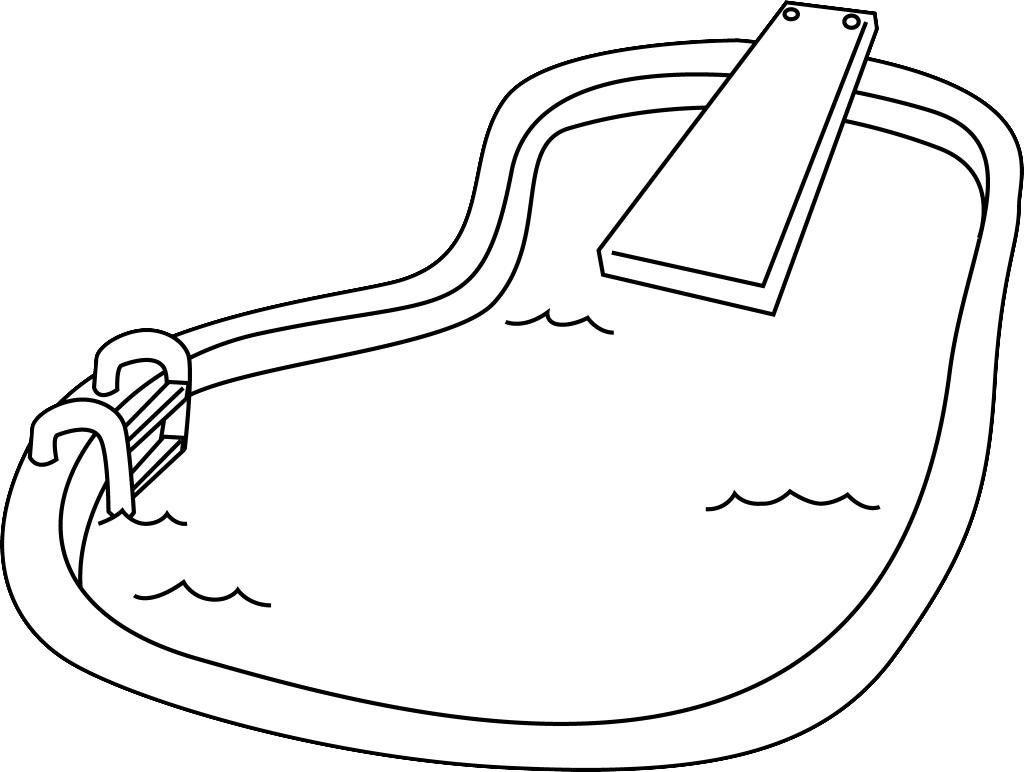
\includegraphics[width=0.4\textwidth]{figs/frontpage/smartpool.png}
\end{minipage}

\vspace{\fill}
\begin{minipage}[l]{\textwidth}
\begin{tabu} to \textwidth{lX[l]}
\textbf{Dato}           &\today\\
\textbf{Vejleder}		&Vejleder navn\\
\end{tabu}
\end{minipage}

\vspace{10pt}
\begin{minipage}[l]{\textwidth}
\tabulinesep=25pt
\begin{tabu} to \textwidth{X[l]X[l]X[l]}
 \makebox[\linewidth]{\hrulefill}\newline Joachim Dam Andersen     \newline 201370248/IKT  
&\makebox[\linewidth]{\hrulefill}\newline Lasse Priebe             \newline 201370248/IKT 
&\makebox[\linewidth]{\hrulefill}\newline Emil Nyborg              \newline 201370248/IKT\\
 \makebox[\linewidth]{\hrulefill}\newline Bjørn Nørgaard Sørensen  \newline 201370248/IKT  
&\makebox[\linewidth]{\hrulefill}\newline Alex Justesen Karlsen    \newline 201370248/IKT 
&\makebox[\linewidth]{\hrulefill}\newline Joachim Händel Noer Wind \newline 201370248/IKT
\end{tabu}
\end{minipage}\clearpage

%% Abstract
% Initial setup
\markboth{RESUMÉ/ABSTRACT}{RESUMÉ/ABSTRACT}
\abstractintoc
\abstractcol
\setlength{\abstitleskip}{-18pt}

% Abstract
\begin{abstract}
Rapporten omhandler et 3. semesterprojekt fra Ingeniørhøjskolen Aarhus Universitet udarbejdet med henblik på at producere et system, som kan fungere som dosering- og sorteringsanlæg til tabletter. Systemet er tiltænkt brug i ældreplejen, som en måde hvorpå fejlmedicinering kan undgås, og tabletsortering kan klares automatisk. Ydermere vil systemet kunne gøre personale og pårørende opmærksomme på, at brugeren ikke har afhentet sine tabletter, indenfor et givet tidsrum. Dette skal formidles ved hjælp af en Android applikation. Systemet og serveren samarbejder om at kontrollerer, hvad der dispenseres til den specifikke bruger og hvornår. Denne kommunikation er ikke fuldt ud implementeret endnu. Systemet var oprindeligt tiltænkt brug i private hjem, men undervejs i processen er idéen ændret idet at fokus flyttes fra private hjem til brug i plejesektoren. 
Produktet kan på nuværende tidspunkt dosere et bestemt antal tabletter af én enkelt type. Systemet har på nuværende tidspunkt allerede implementeret muligheden for at udvide med ekstra dispenserer, og er derfor velegnet til videreudvikling. 
Til systemet er der implementeret en fungerende brugergrænseflade, som er testet med en brugervenlighedsundersøgelse, der ved adspørgelse af 15 studerende har påpeget adskillige muligheder for forbedring.
Under systemudviklingen er den største arbejdsindsats lagt i undersøgelse af teknologier og mulige løsningsforslag.
\end{abstract}

\begin{abstracten}
The report covers a third semesterproject from the Aarhus University School of Engineering. The goal is to produce a system that can function as a dispensing and sorting machine for pills. The system is intended for use in eldercare, as a way of preventing medication errors and a way of sorting pills automaticly. Furthermore, the system will be able to notify staff and relatives if the elder has not picked up their pills, within a given timeperiod. The staff and relatives will be notified via an Android application. The system and a server operate together in order to control what is dispensed to whom and when. Though this communication is not fully implemented yet. The system was originally intended for use in private homes, but during the process, the idea evolved so that the focus was changed from home use to the healthcare sector.
The product can at this time dispense a certain number of pills which will have to be of a single type. The option of adding extra dispensers is already implemented, and is therefore suitable for further development.
The system also has a functioning interface implemented, which has been tested with a user-experience study in which 15 students participated. With the feedback made several things clear, and several of these are suitable for further work.
During the system development the largest effort was put into the study of technologies and potential solutions for the problem chosen.
\end{abstracten}\clearpage

%% Forord
\pagestyle{asereport}
\chapter{Forord}

% Forordet benyttes til at informere kort om visse ydre omstændigheder for projektet, såsom projekttype og hvor projektet er gennemført, historisk baggrund (andre arbejder, som har givet anledning til det aktuelle projekt) og hvor inspirationen og ideen er kommet fra, m.v.

Dette dokument er sammensat for at dokumentere arbejdet på 4. semesterprojektet for retningen IKT på ingeniørhøjskolen Århus.

Der vil i denne rapport være referencer til bilag og dokumentation, som det ikke ville være hensigtsmæssigt at medtage. Samtlige bilag m.m. vil være at finde på den vedlagt CD-rom. 

Source kode til projektet kan findes på CD'en. Link til vores github repo følger her: \newline \url{https://github.com/BjornNorgaard/DuckMaster3001}

\vspace{5mm}

\large{\textit{En stor tak til}}

\begin{displayquote}
    Lars Mortensen for god og brugbar vejledning.
\end{displayquote}

\begin{displayquote}
    Stjerne Apoteket for at lade gruppen komme på besøg og se deres sorteringsmaskine.
\end{displayquote}

\begin{displayquote}
    Sofie Fredslund for at lade os interviewe hende til projektet.
\end{displayquote}

\begin{displayquote}
   Underviserne på ASE, for hjælp og vejledning.
\end{displayquote}

\clearpage

%% ToC
\tableofcontents\clearpage

\mainmatter

%% Todo oversigt - SKAL UDKOMMENTERES FØR AFLEVERING
\listoftodos[Liste over gøremål]

%% Indledning
\chapter{Indledning}

Hello \cite{fysikbog} og sådan kan det jo gå.\clearpage

%% Projektformulering
\documentclass[a4paper,11pt,oneside]{memoir}
%!TEX root = main.tex
% Encoding
%\usepackage[utf8]{inputenc} % pdfLatex
\usepackage[T1]{fontenc}
\usepackage[danish]{babel}
\renewcommand{\danishhyphenmins}{22}
\usepackage[utf8]{inputenc} % æ ø å

% Date
\usepackage[ddmmyyyy]{datetime}
\renewcommand{\dateseparator}{.}

% Fonts
\usepackage{fourier}
\usepackage[scaled=0.8]{beramono}

% Math
\usepackage{amsmath,amssymb}
\usepackage{bm}
\usepackage{amsthm}
\usepackage{mathtools}

% Graphics
\usepackage[usenames,dvipsnames,table]{xcolor}
\usepackage{graphicx}
\usepackage{float}
%\usepackage[section]{placeins}
\usepackage{tikz}
\usepackage[pages=some]{background}
\usepackage{wrapfig}

% Listings & Tables
\usepackage{listings}
%\usepackage{pythontex}
\usepackage{enumitem}
\usepackage{tabu}
\usepackage{longtable}
\usepackage{multirow}
\usepackage{makecell}


% References & Quotes
%\usepackage[danish]{varioref}				% Muliggoer bl.a. krydshenvisninger med sidetal (\vref)
%\usepackage{nat}							% Udvidelse med naturvidenskabelige citationsmodeller
\usepackage[danish=guillemets]{csquotes}
\usepackage[hidelinks]{hyperref}
\hypersetup{
    pdfstartview={FitH},
    pdftitle={Smart Pool 2.0},
    pdfsubject={Projektrapport},
    pdfauthor={I4PRJ4GRP3}
}
\usepackage[all]{hypcap}

% Etc
\usepackage[
	%backend=biber,
	backend=bibtex,
	style=ieee,
	natbib=true,
	backref=false,
	backrefstyle=all+,
	hyperref=true
]{biblatex}
\usepackage{pdflscape}
\usepackage[nomain,toc,xindy,acronym,nonumberlist,noredefwarn]{glossaries}
\usepackage[xindy]{imakeidx}
\usepackage{float}
\makeindex

% Dummy
\usepackage{lipsum}
%!TEX root = main.tex
% Page setup
\setulmarginsandblock{35mm}{25mm}{*}
\setlrmarginsandblock{20mm}{20mm}{*}
\setheadfoot{4\onelineskip}{2\onelineskip}
\setheaderspaces{*}{5mm}{*}
\checkandfixthelayout

% Pagestyle
\makepagestyle{asereport}
	\makeevenhead{asereport}{}{}{}
	\makeoddhead{asereport}{
\includegraphics{figs/frontpage/aseaulogo.pdf}}{}{\small\rightmark{} | \textbf{\thepage{}\vspace{7pt}}}
	\makeevenfoot{asereport}{}{}{}
	\makeoddfoot{asereport}{}{}{}

\makepsmarks{asereport}{
	\createmark{chapter}{both}{shownumber}{}{. \ }
	\createmark{section}{both}{shownumber}{}{. \ }
	\createmark{subsection}{both}{shownumber}{}{. \ }
	\createplainmark{toc}{both}{\contentsname}
	\createplainmark{lof}{both}{\listfigurename}
	\createplainmark{lot}{both}{\listtablename}
	\createplainmark{bib}{both}{\bibname}
	\createplainmark{index}{both}{\indexname}
	\createplainmark{glossary}{both}{\glossaryname}
}

\aliaspagestyle{part}{asereport}
\aliaspagestyle{chapter}{asereport}
\chapterstyle{tandh}

% Modification to certain spacing
\setlength{\parskip}{8pt}
\setlength{\parindent}{0pt}
\setlength{\abovecaptionskip}{7pt}
\setlength{\belowcaptionskip}{-10pt}
\OnehalfSpacing

% Tabu
%\taburowcolors[1]2{white .. light-gray}
\tabulinesep=4pt

% Itemize/enumerate
\setlist{
    before=\vspace{-3pt}, 
    after=\vspace{-3pt},
    itemsep=0pt,
    leftmargin=25pt,
    labelsep=10pt,
    topsep=0pt,
}

% Kommandoer til UC - fixer spacing
% Aktører
\newcommand{\fua}[1]{
	\begin{minipage}[t]{\linewidth}
		\setlist{
		    leftmargin=22pt,
		    itemsep=0pt,
		    topsep=0pt,
		    parsep=3pt
		}
	\begin{itemize}[before={\vspace{-6pt}}, after={\vspace{6pt}}]
	#1
	\end{itemize}
	\end{minipage}
}

% Hovedforløb
\newcommand{\fu}[1]{
\begin{minipage}[t]{\linewidth}
\setlist{
    leftmargin=22pt,
    itemsep=0pt,
    topsep=0pt,
    parsep=3pt
}
\raggedright
\begin{enumerate}[before={\vspace{-5pt}},after={\vspace{6pt}}]
#1
\end{enumerate}
\end{minipage}}

% Extensions
\newcommand{\fuex}[2]{
\begin{minipage}[t]{\linewidth}
\vspace{-6pt}
\raggedright
\textit{#1}
\begin{enumerate}[leftmargin=22pt,itemsep=0pt,parsep=3pt,before={\vspace{-8pt}}, after={\vspace{20pt}},topsep=8pt]
#2
\end{enumerate}
\end{minipage}
}

% Extensions - Sidste entry
\newcommand{\fuexl}[2]{
\begin{minipage}[t]{\linewidth}
\vspace{-6pt}
\raggedright
\textit{#1}
\begin{enumerate}[leftmargin=22pt,itemsep=0pt,parsep=3pt,before={\vspace{-8pt}}, after={\vspace{3pt}},topsep=8pt]
#2
\end{enumerate}
\end{minipage}}

% Versionshistorik
\newcommand{\verhistitem}[2]{
\begin{minipage}[t]{\linewidth}
\vspace{-6pt}
\raggedright
#1
\begin{itemize}[leftmargin=22pt,itemsep=0pt,parsep=0pt,before={\vspace{-10pt}},after={\vspace{3pt}},topsep=8pt]
#2
\end{itemize}
\end{minipage}}

\newcommand{\tverb}[1]{{\texttt{#1}}}

\newcommand{\cond}[1]{
\begin{itemize}[label=,noitemsep,topsep=0pt,after={\vspace*{-\baselineskip}}]
#1
\end{itemize}}

% Etc
\definecolor{light-gray}{gray}{0.8}
\definecolor{pantone}{RGB}{0,61,133}

\setfloatlocations{figure}{H}
\setfloatlocations{table}{H}

\numberwithin{equation}{chapter}
\numberwithin{figure}{chapter}
\setcounter{secnumdepth}{3}
\setcounter{tocdepth}{2}
\maxsecnumdepth{subsection}

\renewcommand*{\cftdotsep}{1}
\setpnumwidth{2em}
\setrmarg{2em}

\setverbatimfont{\ttfamily}

%\renewcommand\cftchaptername {\chaptername~}
%\renewcommand\cftappendixname {\appendixname~}
\addto\captionsdanish{
    \renewcommand\contentsname{Indholdsfortegnelse}
    \renewcommand\appendixname{Appendiks}
}
\renewcommand\appendixpagename{Appendiks}
\renewcommand\appendixtocname{Appendiks}
\newsubfloat{figure}

% Abstract
\newenvironment{abstracten}
{\renewcommand{\abstractname}{Abstract}\abstract}
{\endabstract}
\renewcommand{\abstractnamefont}{\normalfont\Large\bfseries}
%!TEX root = main.tex
% Listings
\AtBeginDocument{%
  \counterwithin*{lstlisting}{section}
  \counterwithin*{lstlisting}{subsection}
  \counterwithin*{lstlisting}{subsubsection}
  \renewcommand{\thelstlisting}{%
    \ifnum\value{subsection}=0
      \thesection.\arabic{lstlisting}%
    \else
      \ifnum\value{subsubsection}=0
        \thesubsection.\arabic{lstlisting}%
      \else
        \thesubsubsection.\arabic{lstlisting}%
      \fi
    \fi
  }
}

% Loading languages
\lstloadlanguages{C, C++}

% Listing setup
\lstdefinestyle{all}{
    basicstyle    = \ttfamily\SingleSpacing\scriptsize,
    numbers       = left, 
    numberstyle   = \ttfamily\tiny,
    breaklines    = true,
    commentstyle=\color{green},
    %backgroundcolor = \color{red},
    numbersep     = 20pt,
    xleftmargin   = \parindent,
    captionpos    = b,
    keywordstyle  = [1]\color{Blue}\bfseries,
    commentstyle  = \itshape\color{Green},
    tabsize       = 3
}

\lstset{
    style = all
} 
%!TEX root = main.tex
\makenoidxglossaries
\newglossaryentry{gui}{
    name={GUI}, 
    description={Graphical User Interface er en brugergrænseflade. Brugerens måde at tilgå systemet på}}

\newglossaryentry{psoc}{
    name={PSoC}, 
    description={PSoC (Programmable System-on-Chip) er et microcontroller system produceret af Cypress Semiconductor}}

\newglossaryentry{moscow}{
    name={MoSCoW}, 
    description={MoSCoW er en metode til at prioritere krav til ens system}}

\newglossaryentry{furps}{
    name={FURPS}, 
    description={FURPS er en metode til kategorisering af systemets ikke-funktionelle krav}}

\newglossaryentry{BDD}{
    name={BDD}, 
    description={BDD (Block Definition Diagram) er et diagram, som beskriver et system ved at opdele det op i mindre blokke}}

\newglossaryentry{IBD}{
    name={IBD}, 
    description={IBD (Internal Block Diagram) er et diagram, som viser forbindelserne mellem blokkene, som kan findes i et BDD}}

\newglossaryentry{pilleskuffe}{
    name={Pilleskuffe},
    description={Skuffen under dispenseren, hvor i den nederste pille ligger i. Skuffen tømmes ved at elektromagneten trækker skuffen til sig.}}

\newglossaryentry{pilledispenser}{
    name={Pilledispenser},
    description={Det rør som pillerne bliver opbevaret i.}}

\newglossaryentry{elektromagneten}{
    name={Elektromagneten},
    description={Elektromagneten er en spole der sendes strøm igennem. Når der er strøm på spolen dannes et magnetfelt. Der vil ofte være tale om det samme hvad enten der står spole eller elektromagnet.}}

%% Forside variabler
\newcommand{\Kursus}{I4PRJ4 F16}
\newcommand{\Projektnavn}{SmartPool 2.0}
\newcommand{\Gruppe}{Gruppe 3}
\newcommand{\Projektdokument}{Projektrapport}

%% Litteratur
\nocite{*}
%\bibliographystyle{harvard}
\bibliography{utils/litteratur}

\begin{document}
\frontmatter

%!TEX root = main.tex
\pagestyle{titlingpage}
\backgroundsetup{
	scale=1,
	angle=0,
	opacity=1,
	contents={
		\begin{tikzpicture}[remember picture,overlay]
		\path [fill=pantone] (-0.5\paperwidth,0.36\paperheight) rectangle (0.5\paperwidth,0.47\paperheight);  
		\path [fill=pantone] (-0.5\paperwidth,-0.47\paperheight) rectangle (0.5\paperwidth,-0.43\paperheight);  
		\end{tikzpicture}}}
\BgThispage
\vspace*{-25mm}
\begin{minipage}[l]{\textwidth}
	
\includegraphics[width=0.75\textwidth]{figs/frontpage/aseaulogohvid.pdf}
\end{minipage}

\vspace{35pt}
\begin{minipage}[l]{\textwidth}
\tabulinesep=10pt
\begin{tabu} to \textwidth{X[l]}
	{\small\MakeUppercase\Kursus}\\
	{\HUGE\bfseries\MakeUppercase\Projektnavn}\\
	{\Large\Gruppe}\\
	{\itshape\Projektdokument}
\end{tabu}
\end{minipage}

\vspace{5pt}
\begin{minipage}[l]{\textwidth}
    \centering
	\vspace*{0cm}\hspace*{8cm}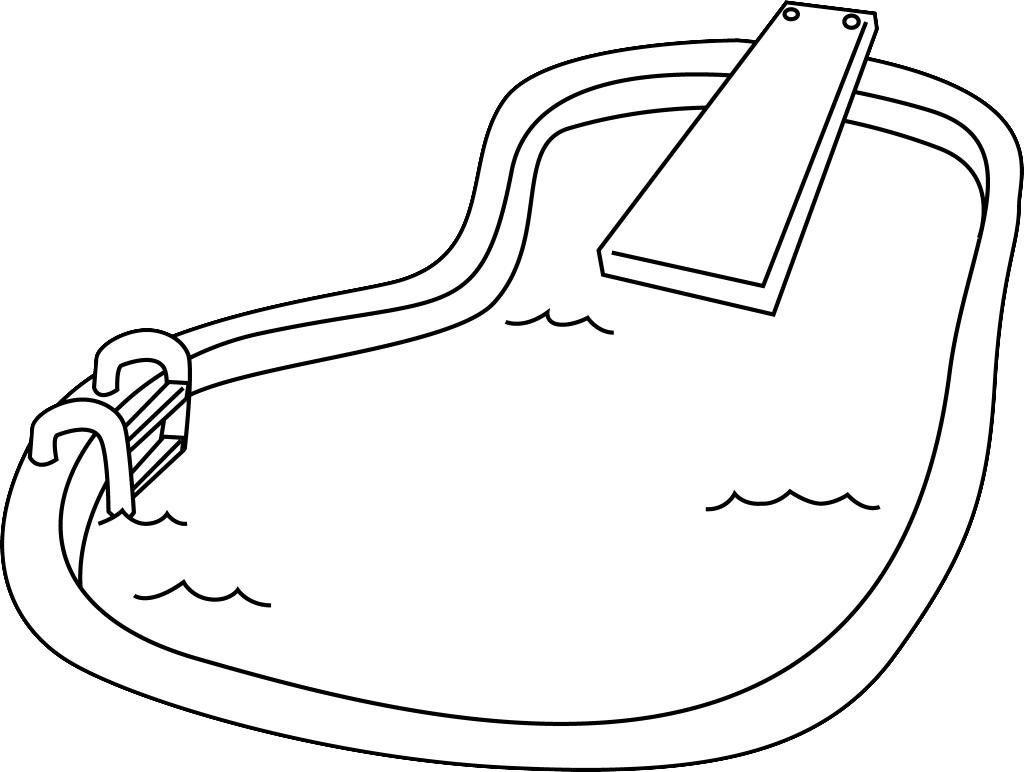
\includegraphics[width=0.4\textwidth]{figs/frontpage/smartpool.png}
\end{minipage}

\vspace{\fill}
\begin{minipage}[l]{\textwidth}
\begin{tabu} to \textwidth{lX[l]}
\textbf{Dato}           &\today\\
\textbf{Vejleder}		&Vejleder navn\\
\end{tabu}
\end{minipage}

\vspace{10pt}
\begin{minipage}[l]{\textwidth}
\tabulinesep=25pt
\begin{tabu} to \textwidth{X[l]X[l]X[l]}
 \makebox[\linewidth]{\hrulefill}\newline Joachim Dam Andersen     \newline 201370248/IKT  
&\makebox[\linewidth]{\hrulefill}\newline Lasse Priebe             \newline 201370248/IKT 
&\makebox[\linewidth]{\hrulefill}\newline Emil Nyborg              \newline 201370248/IKT\\
 \makebox[\linewidth]{\hrulefill}\newline Bjørn Nørgaard Sørensen  \newline 201370248/IKT  
&\makebox[\linewidth]{\hrulefill}\newline Alex Justesen Karlsen    \newline 201370248/IKT 
&\makebox[\linewidth]{\hrulefill}\newline Joachim Händel Noer Wind \newline 201370248/IKT
\end{tabu}
\end{minipage}\clearpage

%% Abstract
% Initial setup
\markboth{RESUMÉ/ABSTRACT}{RESUMÉ/ABSTRACT}
\abstractintoc
\abstractcol
\setlength{\abstitleskip}{-18pt}

% Abstract
\begin{abstract}
Rapporten omhandler et 3. semesterprojekt fra Ingeniørhøjskolen Aarhus Universitet udarbejdet med henblik på at producere et system, som kan fungere som dosering- og sorteringsanlæg til tabletter. Systemet er tiltænkt brug i ældreplejen, som en måde hvorpå fejlmedicinering kan undgås, og tabletsortering kan klares automatisk. Ydermere vil systemet kunne gøre personale og pårørende opmærksomme på, at brugeren ikke har afhentet sine tabletter, indenfor et givet tidsrum. Dette skal formidles ved hjælp af en Android applikation. Systemet og serveren samarbejder om at kontrollerer, hvad der dispenseres til den specifikke bruger og hvornår. Denne kommunikation er ikke fuldt ud implementeret endnu. Systemet var oprindeligt tiltænkt brug i private hjem, men undervejs i processen er idéen ændret idet at fokus flyttes fra private hjem til brug i plejesektoren. 
Produktet kan på nuværende tidspunkt dosere et bestemt antal tabletter af én enkelt type. Systemet har på nuværende tidspunkt allerede implementeret muligheden for at udvide med ekstra dispenserer, og er derfor velegnet til videreudvikling. 
Til systemet er der implementeret en fungerende brugergrænseflade, som er testet med en brugervenlighedsundersøgelse, der ved adspørgelse af 15 studerende har påpeget adskillige muligheder for forbedring.
Under systemudviklingen er den største arbejdsindsats lagt i undersøgelse af teknologier og mulige løsningsforslag.
\end{abstract}

\begin{abstracten}
The report covers a third semesterproject from the Aarhus University School of Engineering. The goal is to produce a system that can function as a dispensing and sorting machine for pills. The system is intended for use in eldercare, as a way of preventing medication errors and a way of sorting pills automaticly. Furthermore, the system will be able to notify staff and relatives if the elder has not picked up their pills, within a given timeperiod. The staff and relatives will be notified via an Android application. The system and a server operate together in order to control what is dispensed to whom and when. Though this communication is not fully implemented yet. The system was originally intended for use in private homes, but during the process, the idea evolved so that the focus was changed from home use to the healthcare sector.
The product can at this time dispense a certain number of pills which will have to be of a single type. The option of adding extra dispensers is already implemented, and is therefore suitable for further development.
The system also has a functioning interface implemented, which has been tested with a user-experience study in which 15 students participated. With the feedback made several things clear, and several of these are suitable for further work.
During the system development the largest effort was put into the study of technologies and potential solutions for the problem chosen.
\end{abstracten}\clearpage

%% Forord
\pagestyle{asereport}
\chapter{Forord}

% Forordet benyttes til at informere kort om visse ydre omstændigheder for projektet, såsom projekttype og hvor projektet er gennemført, historisk baggrund (andre arbejder, som har givet anledning til det aktuelle projekt) og hvor inspirationen og ideen er kommet fra, m.v.

Dette dokument er sammensat for at dokumentere arbejdet på 4. semesterprojektet for retningen IKT på ingeniørhøjskolen Århus.

Der vil i denne rapport være referencer til bilag og dokumentation, som det ikke ville være hensigtsmæssigt at medtage. Samtlige bilag m.m. vil være at finde på den vedlagt CD-rom. 

Source kode til projektet kan findes på CD'en. Link til vores github repo følger her: \newline \url{https://github.com/BjornNorgaard/DuckMaster3001}

\vspace{5mm}

\large{\textit{En stor tak til}}

\begin{displayquote}
    Lars Mortensen for god og brugbar vejledning.
\end{displayquote}

\begin{displayquote}
    Stjerne Apoteket for at lade gruppen komme på besøg og se deres sorteringsmaskine.
\end{displayquote}

\begin{displayquote}
    Sofie Fredslund for at lade os interviewe hende til projektet.
\end{displayquote}

\begin{displayquote}
   Underviserne på ASE, for hjælp og vejledning.
\end{displayquote}

\clearpage

%% ToC
\tableofcontents\clearpage

\mainmatter

%% Todo oversigt - SKAL UDKOMMENTERES FØR AFLEVERING
\listoftodos[Liste over gøremål]

%% Indledning
\chapter{Indledning}

Hello \cite{fysikbog} og sådan kan det jo gå.\clearpage

%% Projektformulering
\documentclass[a4paper,11pt,oneside]{memoir}
\input{utils/packages}
\input{utils/layout}
\input{utils/listings}
\input{utils/ordliste}

%% Forside variabler
\newcommand{\Kursus}{I4PRJ4 F16}
\newcommand{\Projektnavn}{SmartPool 2.0}
\newcommand{\Gruppe}{Gruppe 3}
\newcommand{\Projektdokument}{Projektrapport}

%% Litteratur
\nocite{*}
%\bibliographystyle{harvard}
\bibliography{utils/litteratur}

\begin{document}
\frontmatter

\input{utils/frontpage}\clearpage

%% Abstract
\input{docs/frontmatter/abstract}\clearpage

%% Forord
\pagestyle{asereport}
\input{docs/frontmatter/forord}\clearpage

%% ToC
\tableofcontents\clearpage

\mainmatter

%% Todo oversigt - SKAL UDKOMMENTERES FØR AFLEVERING
\listoftodos[Liste over gøremål]

%% Indledning
\input{docs/frontmatter/indledning}\clearpage

%% Projektformulering
\input{docs/projektformulering/main}\clearpage

%% Kravspecifikation
\input{docs/kravspecifikation/main}\clearpage

%% Systemarkitektur
\input{docs/systemarkitektur/main}\clearpage

%% Processbeskrivelse
\input{docs/processbeskrivelse/main}\clearpage

%% Design
\input{docs/design/main}\clearpage

%% Implementering
\input{docs/implementering/main}\clearpage

%% Integration
\input{docs/integration/main}\clearpage

%% Accepttest
\input{docs/accepttest/main}\clearpage

%% Appendix
\input{docs/appendix/main}\clearpage

\backmatter
%% Glossary
\setglossarystyle{list}
\printnoidxglossary[title=Ordliste]

% Bibliography
\clearpage
\printbibliography[title={Litteratur}]
\end{document}\clearpage

%% Kravspecifikation
\documentclass[a4paper,11pt,oneside]{memoir}
\input{utils/packages}
\input{utils/layout}
\input{utils/listings}
\input{utils/ordliste}

%% Forside variabler
\newcommand{\Kursus}{I4PRJ4 F16}
\newcommand{\Projektnavn}{SmartPool 2.0}
\newcommand{\Gruppe}{Gruppe 3}
\newcommand{\Projektdokument}{Projektrapport}

%% Litteratur
\nocite{*}
%\bibliographystyle{harvard}
\bibliography{utils/litteratur}

\begin{document}
\frontmatter

\input{utils/frontpage}\clearpage

%% Abstract
\input{docs/frontmatter/abstract}\clearpage

%% Forord
\pagestyle{asereport}
\input{docs/frontmatter/forord}\clearpage

%% ToC
\tableofcontents\clearpage

\mainmatter

%% Todo oversigt - SKAL UDKOMMENTERES FØR AFLEVERING
\listoftodos[Liste over gøremål]

%% Indledning
\input{docs/frontmatter/indledning}\clearpage

%% Projektformulering
\input{docs/projektformulering/main}\clearpage

%% Kravspecifikation
\input{docs/kravspecifikation/main}\clearpage

%% Systemarkitektur
\input{docs/systemarkitektur/main}\clearpage

%% Processbeskrivelse
\input{docs/processbeskrivelse/main}\clearpage

%% Design
\input{docs/design/main}\clearpage

%% Implementering
\input{docs/implementering/main}\clearpage

%% Integration
\input{docs/integration/main}\clearpage

%% Accepttest
\input{docs/accepttest/main}\clearpage

%% Appendix
\input{docs/appendix/main}\clearpage

\backmatter
%% Glossary
\setglossarystyle{list}
\printnoidxglossary[title=Ordliste]

% Bibliography
\clearpage
\printbibliography[title={Litteratur}]
\end{document}\clearpage

%% Systemarkitektur
\documentclass[a4paper,11pt,oneside]{memoir}
\input{utils/packages}
\input{utils/layout}
\input{utils/listings}
\input{utils/ordliste}

%% Forside variabler
\newcommand{\Kursus}{I4PRJ4 F16}
\newcommand{\Projektnavn}{SmartPool 2.0}
\newcommand{\Gruppe}{Gruppe 3}
\newcommand{\Projektdokument}{Projektrapport}

%% Litteratur
\nocite{*}
%\bibliographystyle{harvard}
\bibliography{utils/litteratur}

\begin{document}
\frontmatter

\input{utils/frontpage}\clearpage

%% Abstract
\input{docs/frontmatter/abstract}\clearpage

%% Forord
\pagestyle{asereport}
\input{docs/frontmatter/forord}\clearpage

%% ToC
\tableofcontents\clearpage

\mainmatter

%% Todo oversigt - SKAL UDKOMMENTERES FØR AFLEVERING
\listoftodos[Liste over gøremål]

%% Indledning
\input{docs/frontmatter/indledning}\clearpage

%% Projektformulering
\input{docs/projektformulering/main}\clearpage

%% Kravspecifikation
\input{docs/kravspecifikation/main}\clearpage

%% Systemarkitektur
\input{docs/systemarkitektur/main}\clearpage

%% Processbeskrivelse
\input{docs/processbeskrivelse/main}\clearpage

%% Design
\input{docs/design/main}\clearpage

%% Implementering
\input{docs/implementering/main}\clearpage

%% Integration
\input{docs/integration/main}\clearpage

%% Accepttest
\input{docs/accepttest/main}\clearpage

%% Appendix
\input{docs/appendix/main}\clearpage

\backmatter
%% Glossary
\setglossarystyle{list}
\printnoidxglossary[title=Ordliste]

% Bibliography
\clearpage
\printbibliography[title={Litteratur}]
\end{document}\clearpage

%% Processbeskrivelse
\documentclass[a4paper,11pt,oneside]{memoir}
\input{utils/packages}
\input{utils/layout}
\input{utils/listings}
\input{utils/ordliste}

%% Forside variabler
\newcommand{\Kursus}{I4PRJ4 F16}
\newcommand{\Projektnavn}{SmartPool 2.0}
\newcommand{\Gruppe}{Gruppe 3}
\newcommand{\Projektdokument}{Projektrapport}

%% Litteratur
\nocite{*}
%\bibliographystyle{harvard}
\bibliography{utils/litteratur}

\begin{document}
\frontmatter

\input{utils/frontpage}\clearpage

%% Abstract
\input{docs/frontmatter/abstract}\clearpage

%% Forord
\pagestyle{asereport}
\input{docs/frontmatter/forord}\clearpage

%% ToC
\tableofcontents\clearpage

\mainmatter

%% Todo oversigt - SKAL UDKOMMENTERES FØR AFLEVERING
\listoftodos[Liste over gøremål]

%% Indledning
\input{docs/frontmatter/indledning}\clearpage

%% Projektformulering
\input{docs/projektformulering/main}\clearpage

%% Kravspecifikation
\input{docs/kravspecifikation/main}\clearpage

%% Systemarkitektur
\input{docs/systemarkitektur/main}\clearpage

%% Processbeskrivelse
\input{docs/processbeskrivelse/main}\clearpage

%% Design
\input{docs/design/main}\clearpage

%% Implementering
\input{docs/implementering/main}\clearpage

%% Integration
\input{docs/integration/main}\clearpage

%% Accepttest
\input{docs/accepttest/main}\clearpage

%% Appendix
\input{docs/appendix/main}\clearpage

\backmatter
%% Glossary
\setglossarystyle{list}
\printnoidxglossary[title=Ordliste]

% Bibliography
\clearpage
\printbibliography[title={Litteratur}]
\end{document}\clearpage

%% Design
\documentclass[a4paper,11pt,oneside]{memoir}
\input{utils/packages}
\input{utils/layout}
\input{utils/listings}
\input{utils/ordliste}

%% Forside variabler
\newcommand{\Kursus}{I4PRJ4 F16}
\newcommand{\Projektnavn}{SmartPool 2.0}
\newcommand{\Gruppe}{Gruppe 3}
\newcommand{\Projektdokument}{Projektrapport}

%% Litteratur
\nocite{*}
%\bibliographystyle{harvard}
\bibliography{utils/litteratur}

\begin{document}
\frontmatter

\input{utils/frontpage}\clearpage

%% Abstract
\input{docs/frontmatter/abstract}\clearpage

%% Forord
\pagestyle{asereport}
\input{docs/frontmatter/forord}\clearpage

%% ToC
\tableofcontents\clearpage

\mainmatter

%% Todo oversigt - SKAL UDKOMMENTERES FØR AFLEVERING
\listoftodos[Liste over gøremål]

%% Indledning
\input{docs/frontmatter/indledning}\clearpage

%% Projektformulering
\input{docs/projektformulering/main}\clearpage

%% Kravspecifikation
\input{docs/kravspecifikation/main}\clearpage

%% Systemarkitektur
\input{docs/systemarkitektur/main}\clearpage

%% Processbeskrivelse
\input{docs/processbeskrivelse/main}\clearpage

%% Design
\input{docs/design/main}\clearpage

%% Implementering
\input{docs/implementering/main}\clearpage

%% Integration
\input{docs/integration/main}\clearpage

%% Accepttest
\input{docs/accepttest/main}\clearpage

%% Appendix
\input{docs/appendix/main}\clearpage

\backmatter
%% Glossary
\setglossarystyle{list}
\printnoidxglossary[title=Ordliste]

% Bibliography
\clearpage
\printbibliography[title={Litteratur}]
\end{document}\clearpage

%% Implementering
\documentclass[a4paper,11pt,oneside]{memoir}
\input{utils/packages}
\input{utils/layout}
\input{utils/listings}
\input{utils/ordliste}

%% Forside variabler
\newcommand{\Kursus}{I4PRJ4 F16}
\newcommand{\Projektnavn}{SmartPool 2.0}
\newcommand{\Gruppe}{Gruppe 3}
\newcommand{\Projektdokument}{Projektrapport}

%% Litteratur
\nocite{*}
%\bibliographystyle{harvard}
\bibliography{utils/litteratur}

\begin{document}
\frontmatter

\input{utils/frontpage}\clearpage

%% Abstract
\input{docs/frontmatter/abstract}\clearpage

%% Forord
\pagestyle{asereport}
\input{docs/frontmatter/forord}\clearpage

%% ToC
\tableofcontents\clearpage

\mainmatter

%% Todo oversigt - SKAL UDKOMMENTERES FØR AFLEVERING
\listoftodos[Liste over gøremål]

%% Indledning
\input{docs/frontmatter/indledning}\clearpage

%% Projektformulering
\input{docs/projektformulering/main}\clearpage

%% Kravspecifikation
\input{docs/kravspecifikation/main}\clearpage

%% Systemarkitektur
\input{docs/systemarkitektur/main}\clearpage

%% Processbeskrivelse
\input{docs/processbeskrivelse/main}\clearpage

%% Design
\input{docs/design/main}\clearpage

%% Implementering
\input{docs/implementering/main}\clearpage

%% Integration
\input{docs/integration/main}\clearpage

%% Accepttest
\input{docs/accepttest/main}\clearpage

%% Appendix
\input{docs/appendix/main}\clearpage

\backmatter
%% Glossary
\setglossarystyle{list}
\printnoidxglossary[title=Ordliste]

% Bibliography
\clearpage
\printbibliography[title={Litteratur}]
\end{document}\clearpage

%% Integration
\documentclass[a4paper,11pt,oneside]{memoir}
\input{utils/packages}
\input{utils/layout}
\input{utils/listings}
\input{utils/ordliste}

%% Forside variabler
\newcommand{\Kursus}{I4PRJ4 F16}
\newcommand{\Projektnavn}{SmartPool 2.0}
\newcommand{\Gruppe}{Gruppe 3}
\newcommand{\Projektdokument}{Projektrapport}

%% Litteratur
\nocite{*}
%\bibliographystyle{harvard}
\bibliography{utils/litteratur}

\begin{document}
\frontmatter

\input{utils/frontpage}\clearpage

%% Abstract
\input{docs/frontmatter/abstract}\clearpage

%% Forord
\pagestyle{asereport}
\input{docs/frontmatter/forord}\clearpage

%% ToC
\tableofcontents\clearpage

\mainmatter

%% Todo oversigt - SKAL UDKOMMENTERES FØR AFLEVERING
\listoftodos[Liste over gøremål]

%% Indledning
\input{docs/frontmatter/indledning}\clearpage

%% Projektformulering
\input{docs/projektformulering/main}\clearpage

%% Kravspecifikation
\input{docs/kravspecifikation/main}\clearpage

%% Systemarkitektur
\input{docs/systemarkitektur/main}\clearpage

%% Processbeskrivelse
\input{docs/processbeskrivelse/main}\clearpage

%% Design
\input{docs/design/main}\clearpage

%% Implementering
\input{docs/implementering/main}\clearpage

%% Integration
\input{docs/integration/main}\clearpage

%% Accepttest
\input{docs/accepttest/main}\clearpage

%% Appendix
\input{docs/appendix/main}\clearpage

\backmatter
%% Glossary
\setglossarystyle{list}
\printnoidxglossary[title=Ordliste]

% Bibliography
\clearpage
\printbibliography[title={Litteratur}]
\end{document}\clearpage

%% Accepttest
\documentclass[a4paper,11pt,oneside]{memoir}
\input{utils/packages}
\input{utils/layout}
\input{utils/listings}
\input{utils/ordliste}

%% Forside variabler
\newcommand{\Kursus}{I4PRJ4 F16}
\newcommand{\Projektnavn}{SmartPool 2.0}
\newcommand{\Gruppe}{Gruppe 3}
\newcommand{\Projektdokument}{Projektrapport}

%% Litteratur
\nocite{*}
%\bibliographystyle{harvard}
\bibliography{utils/litteratur}

\begin{document}
\frontmatter

\input{utils/frontpage}\clearpage

%% Abstract
\input{docs/frontmatter/abstract}\clearpage

%% Forord
\pagestyle{asereport}
\input{docs/frontmatter/forord}\clearpage

%% ToC
\tableofcontents\clearpage

\mainmatter

%% Todo oversigt - SKAL UDKOMMENTERES FØR AFLEVERING
\listoftodos[Liste over gøremål]

%% Indledning
\input{docs/frontmatter/indledning}\clearpage

%% Projektformulering
\input{docs/projektformulering/main}\clearpage

%% Kravspecifikation
\input{docs/kravspecifikation/main}\clearpage

%% Systemarkitektur
\input{docs/systemarkitektur/main}\clearpage

%% Processbeskrivelse
\input{docs/processbeskrivelse/main}\clearpage

%% Design
\input{docs/design/main}\clearpage

%% Implementering
\input{docs/implementering/main}\clearpage

%% Integration
\input{docs/integration/main}\clearpage

%% Accepttest
\input{docs/accepttest/main}\clearpage

%% Appendix
\input{docs/appendix/main}\clearpage

\backmatter
%% Glossary
\setglossarystyle{list}
\printnoidxglossary[title=Ordliste]

% Bibliography
\clearpage
\printbibliography[title={Litteratur}]
\end{document}\clearpage

%% Appendix
\documentclass[a4paper,11pt,oneside]{memoir}
\input{utils/packages}
\input{utils/layout}
\input{utils/listings}
\input{utils/ordliste}

%% Forside variabler
\newcommand{\Kursus}{I4PRJ4 F16}
\newcommand{\Projektnavn}{SmartPool 2.0}
\newcommand{\Gruppe}{Gruppe 3}
\newcommand{\Projektdokument}{Projektrapport}

%% Litteratur
\nocite{*}
%\bibliographystyle{harvard}
\bibliography{utils/litteratur}

\begin{document}
\frontmatter

\input{utils/frontpage}\clearpage

%% Abstract
\input{docs/frontmatter/abstract}\clearpage

%% Forord
\pagestyle{asereport}
\input{docs/frontmatter/forord}\clearpage

%% ToC
\tableofcontents\clearpage

\mainmatter

%% Todo oversigt - SKAL UDKOMMENTERES FØR AFLEVERING
\listoftodos[Liste over gøremål]

%% Indledning
\input{docs/frontmatter/indledning}\clearpage

%% Projektformulering
\input{docs/projektformulering/main}\clearpage

%% Kravspecifikation
\input{docs/kravspecifikation/main}\clearpage

%% Systemarkitektur
\input{docs/systemarkitektur/main}\clearpage

%% Processbeskrivelse
\input{docs/processbeskrivelse/main}\clearpage

%% Design
\input{docs/design/main}\clearpage

%% Implementering
\input{docs/implementering/main}\clearpage

%% Integration
\input{docs/integration/main}\clearpage

%% Accepttest
\input{docs/accepttest/main}\clearpage

%% Appendix
\input{docs/appendix/main}\clearpage

\backmatter
%% Glossary
\setglossarystyle{list}
\printnoidxglossary[title=Ordliste]

% Bibliography
\clearpage
\printbibliography[title={Litteratur}]
\end{document}\clearpage

\backmatter
%% Glossary
\setglossarystyle{list}
\printnoidxglossary[title=Ordliste]

% Bibliography
\clearpage
\printbibliography[title={Litteratur}]
\end{document}\clearpage

%% Kravspecifikation
\documentclass[a4paper,11pt,oneside]{memoir}
%!TEX root = main.tex
% Encoding
%\usepackage[utf8]{inputenc} % pdfLatex
\usepackage[T1]{fontenc}
\usepackage[danish]{babel}
\renewcommand{\danishhyphenmins}{22}
\usepackage[utf8]{inputenc} % æ ø å

% Date
\usepackage[ddmmyyyy]{datetime}
\renewcommand{\dateseparator}{.}

% Fonts
\usepackage{fourier}
\usepackage[scaled=0.8]{beramono}

% Math
\usepackage{amsmath,amssymb}
\usepackage{bm}
\usepackage{amsthm}
\usepackage{mathtools}

% Graphics
\usepackage[usenames,dvipsnames,table]{xcolor}
\usepackage{graphicx}
\usepackage{float}
%\usepackage[section]{placeins}
\usepackage{tikz}
\usepackage[pages=some]{background}
\usepackage{wrapfig}

% Listings & Tables
\usepackage{listings}
%\usepackage{pythontex}
\usepackage{enumitem}
\usepackage{tabu}
\usepackage{longtable}
\usepackage{multirow}
\usepackage{makecell}


% References & Quotes
%\usepackage[danish]{varioref}				% Muliggoer bl.a. krydshenvisninger med sidetal (\vref)
%\usepackage{nat}							% Udvidelse med naturvidenskabelige citationsmodeller
\usepackage[danish=guillemets]{csquotes}
\usepackage[hidelinks]{hyperref}
\hypersetup{
    pdfstartview={FitH},
    pdftitle={Smart Pool 2.0},
    pdfsubject={Projektrapport},
    pdfauthor={I4PRJ4GRP3}
}
\usepackage[all]{hypcap}

% Etc
\usepackage[
	%backend=biber,
	backend=bibtex,
	style=ieee,
	natbib=true,
	backref=false,
	backrefstyle=all+,
	hyperref=true
]{biblatex}
\usepackage{pdflscape}
\usepackage[nomain,toc,xindy,acronym,nonumberlist,noredefwarn]{glossaries}
\usepackage[xindy]{imakeidx}
\usepackage{float}
\makeindex

% Dummy
\usepackage{lipsum}
%!TEX root = main.tex
% Page setup
\setulmarginsandblock{35mm}{25mm}{*}
\setlrmarginsandblock{20mm}{20mm}{*}
\setheadfoot{4\onelineskip}{2\onelineskip}
\setheaderspaces{*}{5mm}{*}
\checkandfixthelayout

% Pagestyle
\makepagestyle{asereport}
	\makeevenhead{asereport}{}{}{}
	\makeoddhead{asereport}{
\includegraphics{figs/frontpage/aseaulogo.pdf}}{}{\small\rightmark{} | \textbf{\thepage{}\vspace{7pt}}}
	\makeevenfoot{asereport}{}{}{}
	\makeoddfoot{asereport}{}{}{}

\makepsmarks{asereport}{
	\createmark{chapter}{both}{shownumber}{}{. \ }
	\createmark{section}{both}{shownumber}{}{. \ }
	\createmark{subsection}{both}{shownumber}{}{. \ }
	\createplainmark{toc}{both}{\contentsname}
	\createplainmark{lof}{both}{\listfigurename}
	\createplainmark{lot}{both}{\listtablename}
	\createplainmark{bib}{both}{\bibname}
	\createplainmark{index}{both}{\indexname}
	\createplainmark{glossary}{both}{\glossaryname}
}

\aliaspagestyle{part}{asereport}
\aliaspagestyle{chapter}{asereport}
\chapterstyle{tandh}

% Modification to certain spacing
\setlength{\parskip}{8pt}
\setlength{\parindent}{0pt}
\setlength{\abovecaptionskip}{7pt}
\setlength{\belowcaptionskip}{-10pt}
\OnehalfSpacing

% Tabu
%\taburowcolors[1]2{white .. light-gray}
\tabulinesep=4pt

% Itemize/enumerate
\setlist{
    before=\vspace{-3pt}, 
    after=\vspace{-3pt},
    itemsep=0pt,
    leftmargin=25pt,
    labelsep=10pt,
    topsep=0pt,
}

% Kommandoer til UC - fixer spacing
% Aktører
\newcommand{\fua}[1]{
	\begin{minipage}[t]{\linewidth}
		\setlist{
		    leftmargin=22pt,
		    itemsep=0pt,
		    topsep=0pt,
		    parsep=3pt
		}
	\begin{itemize}[before={\vspace{-6pt}}, after={\vspace{6pt}}]
	#1
	\end{itemize}
	\end{minipage}
}

% Hovedforløb
\newcommand{\fu}[1]{
\begin{minipage}[t]{\linewidth}
\setlist{
    leftmargin=22pt,
    itemsep=0pt,
    topsep=0pt,
    parsep=3pt
}
\raggedright
\begin{enumerate}[before={\vspace{-5pt}},after={\vspace{6pt}}]
#1
\end{enumerate}
\end{minipage}}

% Extensions
\newcommand{\fuex}[2]{
\begin{minipage}[t]{\linewidth}
\vspace{-6pt}
\raggedright
\textit{#1}
\begin{enumerate}[leftmargin=22pt,itemsep=0pt,parsep=3pt,before={\vspace{-8pt}}, after={\vspace{20pt}},topsep=8pt]
#2
\end{enumerate}
\end{minipage}
}

% Extensions - Sidste entry
\newcommand{\fuexl}[2]{
\begin{minipage}[t]{\linewidth}
\vspace{-6pt}
\raggedright
\textit{#1}
\begin{enumerate}[leftmargin=22pt,itemsep=0pt,parsep=3pt,before={\vspace{-8pt}}, after={\vspace{3pt}},topsep=8pt]
#2
\end{enumerate}
\end{minipage}}

% Versionshistorik
\newcommand{\verhistitem}[2]{
\begin{minipage}[t]{\linewidth}
\vspace{-6pt}
\raggedright
#1
\begin{itemize}[leftmargin=22pt,itemsep=0pt,parsep=0pt,before={\vspace{-10pt}},after={\vspace{3pt}},topsep=8pt]
#2
\end{itemize}
\end{minipage}}

\newcommand{\tverb}[1]{{\texttt{#1}}}

\newcommand{\cond}[1]{
\begin{itemize}[label=,noitemsep,topsep=0pt,after={\vspace*{-\baselineskip}}]
#1
\end{itemize}}

% Etc
\definecolor{light-gray}{gray}{0.8}
\definecolor{pantone}{RGB}{0,61,133}

\setfloatlocations{figure}{H}
\setfloatlocations{table}{H}

\numberwithin{equation}{chapter}
\numberwithin{figure}{chapter}
\setcounter{secnumdepth}{3}
\setcounter{tocdepth}{2}
\maxsecnumdepth{subsection}

\renewcommand*{\cftdotsep}{1}
\setpnumwidth{2em}
\setrmarg{2em}

\setverbatimfont{\ttfamily}

%\renewcommand\cftchaptername {\chaptername~}
%\renewcommand\cftappendixname {\appendixname~}
\addto\captionsdanish{
    \renewcommand\contentsname{Indholdsfortegnelse}
    \renewcommand\appendixname{Appendiks}
}
\renewcommand\appendixpagename{Appendiks}
\renewcommand\appendixtocname{Appendiks}
\newsubfloat{figure}

% Abstract
\newenvironment{abstracten}
{\renewcommand{\abstractname}{Abstract}\abstract}
{\endabstract}
\renewcommand{\abstractnamefont}{\normalfont\Large\bfseries}
%!TEX root = main.tex
% Listings
\AtBeginDocument{%
  \counterwithin*{lstlisting}{section}
  \counterwithin*{lstlisting}{subsection}
  \counterwithin*{lstlisting}{subsubsection}
  \renewcommand{\thelstlisting}{%
    \ifnum\value{subsection}=0
      \thesection.\arabic{lstlisting}%
    \else
      \ifnum\value{subsubsection}=0
        \thesubsection.\arabic{lstlisting}%
      \else
        \thesubsubsection.\arabic{lstlisting}%
      \fi
    \fi
  }
}

% Loading languages
\lstloadlanguages{C, C++}

% Listing setup
\lstdefinestyle{all}{
    basicstyle    = \ttfamily\SingleSpacing\scriptsize,
    numbers       = left, 
    numberstyle   = \ttfamily\tiny,
    breaklines    = true,
    commentstyle=\color{green},
    %backgroundcolor = \color{red},
    numbersep     = 20pt,
    xleftmargin   = \parindent,
    captionpos    = b,
    keywordstyle  = [1]\color{Blue}\bfseries,
    commentstyle  = \itshape\color{Green},
    tabsize       = 3
}

\lstset{
    style = all
} 
%!TEX root = main.tex
\makenoidxglossaries
\newglossaryentry{gui}{
    name={GUI}, 
    description={Graphical User Interface er en brugergrænseflade. Brugerens måde at tilgå systemet på}}

\newglossaryentry{psoc}{
    name={PSoC}, 
    description={PSoC (Programmable System-on-Chip) er et microcontroller system produceret af Cypress Semiconductor}}

\newglossaryentry{moscow}{
    name={MoSCoW}, 
    description={MoSCoW er en metode til at prioritere krav til ens system}}

\newglossaryentry{furps}{
    name={FURPS}, 
    description={FURPS er en metode til kategorisering af systemets ikke-funktionelle krav}}

\newglossaryentry{BDD}{
    name={BDD}, 
    description={BDD (Block Definition Diagram) er et diagram, som beskriver et system ved at opdele det op i mindre blokke}}

\newglossaryentry{IBD}{
    name={IBD}, 
    description={IBD (Internal Block Diagram) er et diagram, som viser forbindelserne mellem blokkene, som kan findes i et BDD}}

\newglossaryentry{pilleskuffe}{
    name={Pilleskuffe},
    description={Skuffen under dispenseren, hvor i den nederste pille ligger i. Skuffen tømmes ved at elektromagneten trækker skuffen til sig.}}

\newglossaryentry{pilledispenser}{
    name={Pilledispenser},
    description={Det rør som pillerne bliver opbevaret i.}}

\newglossaryentry{elektromagneten}{
    name={Elektromagneten},
    description={Elektromagneten er en spole der sendes strøm igennem. Når der er strøm på spolen dannes et magnetfelt. Der vil ofte være tale om det samme hvad enten der står spole eller elektromagnet.}}

%% Forside variabler
\newcommand{\Kursus}{I4PRJ4 F16}
\newcommand{\Projektnavn}{SmartPool 2.0}
\newcommand{\Gruppe}{Gruppe 3}
\newcommand{\Projektdokument}{Projektrapport}

%% Litteratur
\nocite{*}
%\bibliographystyle{harvard}
\bibliography{utils/litteratur}

\begin{document}
\frontmatter

%!TEX root = main.tex
\pagestyle{titlingpage}
\backgroundsetup{
	scale=1,
	angle=0,
	opacity=1,
	contents={
		\begin{tikzpicture}[remember picture,overlay]
		\path [fill=pantone] (-0.5\paperwidth,0.36\paperheight) rectangle (0.5\paperwidth,0.47\paperheight);  
		\path [fill=pantone] (-0.5\paperwidth,-0.47\paperheight) rectangle (0.5\paperwidth,-0.43\paperheight);  
		\end{tikzpicture}}}
\BgThispage
\vspace*{-25mm}
\begin{minipage}[l]{\textwidth}
	
\includegraphics[width=0.75\textwidth]{figs/frontpage/aseaulogohvid.pdf}
\end{minipage}

\vspace{35pt}
\begin{minipage}[l]{\textwidth}
\tabulinesep=10pt
\begin{tabu} to \textwidth{X[l]}
	{\small\MakeUppercase\Kursus}\\
	{\HUGE\bfseries\MakeUppercase\Projektnavn}\\
	{\Large\Gruppe}\\
	{\itshape\Projektdokument}
\end{tabu}
\end{minipage}

\vspace{5pt}
\begin{minipage}[l]{\textwidth}
    \centering
	\vspace*{0cm}\hspace*{8cm}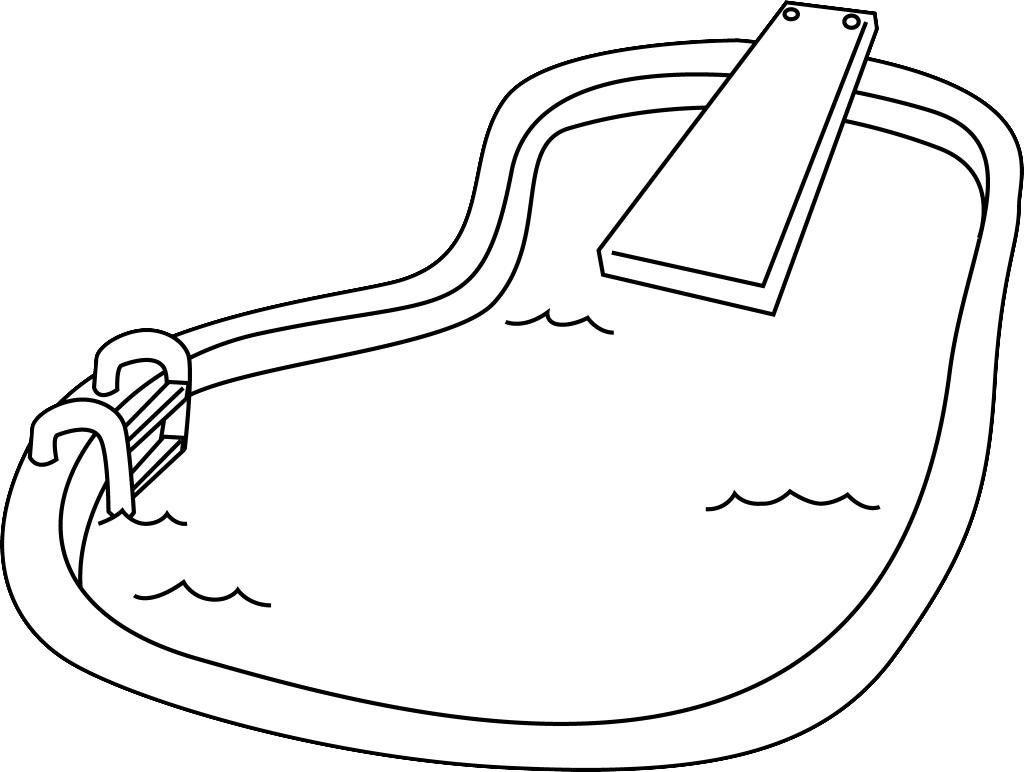
\includegraphics[width=0.4\textwidth]{figs/frontpage/smartpool.png}
\end{minipage}

\vspace{\fill}
\begin{minipage}[l]{\textwidth}
\begin{tabu} to \textwidth{lX[l]}
\textbf{Dato}           &\today\\
\textbf{Vejleder}		&Vejleder navn\\
\end{tabu}
\end{minipage}

\vspace{10pt}
\begin{minipage}[l]{\textwidth}
\tabulinesep=25pt
\begin{tabu} to \textwidth{X[l]X[l]X[l]}
 \makebox[\linewidth]{\hrulefill}\newline Joachim Dam Andersen     \newline 201370248/IKT  
&\makebox[\linewidth]{\hrulefill}\newline Lasse Priebe             \newline 201370248/IKT 
&\makebox[\linewidth]{\hrulefill}\newline Emil Nyborg              \newline 201370248/IKT\\
 \makebox[\linewidth]{\hrulefill}\newline Bjørn Nørgaard Sørensen  \newline 201370248/IKT  
&\makebox[\linewidth]{\hrulefill}\newline Alex Justesen Karlsen    \newline 201370248/IKT 
&\makebox[\linewidth]{\hrulefill}\newline Joachim Händel Noer Wind \newline 201370248/IKT
\end{tabu}
\end{minipage}\clearpage

%% Abstract
% Initial setup
\markboth{RESUMÉ/ABSTRACT}{RESUMÉ/ABSTRACT}
\abstractintoc
\abstractcol
\setlength{\abstitleskip}{-18pt}

% Abstract
\begin{abstract}
Rapporten omhandler et 3. semesterprojekt fra Ingeniørhøjskolen Aarhus Universitet udarbejdet med henblik på at producere et system, som kan fungere som dosering- og sorteringsanlæg til tabletter. Systemet er tiltænkt brug i ældreplejen, som en måde hvorpå fejlmedicinering kan undgås, og tabletsortering kan klares automatisk. Ydermere vil systemet kunne gøre personale og pårørende opmærksomme på, at brugeren ikke har afhentet sine tabletter, indenfor et givet tidsrum. Dette skal formidles ved hjælp af en Android applikation. Systemet og serveren samarbejder om at kontrollerer, hvad der dispenseres til den specifikke bruger og hvornår. Denne kommunikation er ikke fuldt ud implementeret endnu. Systemet var oprindeligt tiltænkt brug i private hjem, men undervejs i processen er idéen ændret idet at fokus flyttes fra private hjem til brug i plejesektoren. 
Produktet kan på nuværende tidspunkt dosere et bestemt antal tabletter af én enkelt type. Systemet har på nuværende tidspunkt allerede implementeret muligheden for at udvide med ekstra dispenserer, og er derfor velegnet til videreudvikling. 
Til systemet er der implementeret en fungerende brugergrænseflade, som er testet med en brugervenlighedsundersøgelse, der ved adspørgelse af 15 studerende har påpeget adskillige muligheder for forbedring.
Under systemudviklingen er den største arbejdsindsats lagt i undersøgelse af teknologier og mulige løsningsforslag.
\end{abstract}

\begin{abstracten}
The report covers a third semesterproject from the Aarhus University School of Engineering. The goal is to produce a system that can function as a dispensing and sorting machine for pills. The system is intended for use in eldercare, as a way of preventing medication errors and a way of sorting pills automaticly. Furthermore, the system will be able to notify staff and relatives if the elder has not picked up their pills, within a given timeperiod. The staff and relatives will be notified via an Android application. The system and a server operate together in order to control what is dispensed to whom and when. Though this communication is not fully implemented yet. The system was originally intended for use in private homes, but during the process, the idea evolved so that the focus was changed from home use to the healthcare sector.
The product can at this time dispense a certain number of pills which will have to be of a single type. The option of adding extra dispensers is already implemented, and is therefore suitable for further development.
The system also has a functioning interface implemented, which has been tested with a user-experience study in which 15 students participated. With the feedback made several things clear, and several of these are suitable for further work.
During the system development the largest effort was put into the study of technologies and potential solutions for the problem chosen.
\end{abstracten}\clearpage

%% Forord
\pagestyle{asereport}
\chapter{Forord}

% Forordet benyttes til at informere kort om visse ydre omstændigheder for projektet, såsom projekttype og hvor projektet er gennemført, historisk baggrund (andre arbejder, som har givet anledning til det aktuelle projekt) og hvor inspirationen og ideen er kommet fra, m.v.

Dette dokument er sammensat for at dokumentere arbejdet på 4. semesterprojektet for retningen IKT på ingeniørhøjskolen Århus.

Der vil i denne rapport være referencer til bilag og dokumentation, som det ikke ville være hensigtsmæssigt at medtage. Samtlige bilag m.m. vil være at finde på den vedlagt CD-rom. 

Source kode til projektet kan findes på CD'en. Link til vores github repo følger her: \newline \url{https://github.com/BjornNorgaard/DuckMaster3001}

\vspace{5mm}

\large{\textit{En stor tak til}}

\begin{displayquote}
    Lars Mortensen for god og brugbar vejledning.
\end{displayquote}

\begin{displayquote}
    Stjerne Apoteket for at lade gruppen komme på besøg og se deres sorteringsmaskine.
\end{displayquote}

\begin{displayquote}
    Sofie Fredslund for at lade os interviewe hende til projektet.
\end{displayquote}

\begin{displayquote}
   Underviserne på ASE, for hjælp og vejledning.
\end{displayquote}

\clearpage

%% ToC
\tableofcontents\clearpage

\mainmatter

%% Todo oversigt - SKAL UDKOMMENTERES FØR AFLEVERING
\listoftodos[Liste over gøremål]

%% Indledning
\chapter{Indledning}

Hello \cite{fysikbog} og sådan kan det jo gå.\clearpage

%% Projektformulering
\documentclass[a4paper,11pt,oneside]{memoir}
\input{utils/packages}
\input{utils/layout}
\input{utils/listings}
\input{utils/ordliste}

%% Forside variabler
\newcommand{\Kursus}{I4PRJ4 F16}
\newcommand{\Projektnavn}{SmartPool 2.0}
\newcommand{\Gruppe}{Gruppe 3}
\newcommand{\Projektdokument}{Projektrapport}

%% Litteratur
\nocite{*}
%\bibliographystyle{harvard}
\bibliography{utils/litteratur}

\begin{document}
\frontmatter

\input{utils/frontpage}\clearpage

%% Abstract
\input{docs/frontmatter/abstract}\clearpage

%% Forord
\pagestyle{asereport}
\input{docs/frontmatter/forord}\clearpage

%% ToC
\tableofcontents\clearpage

\mainmatter

%% Todo oversigt - SKAL UDKOMMENTERES FØR AFLEVERING
\listoftodos[Liste over gøremål]

%% Indledning
\input{docs/frontmatter/indledning}\clearpage

%% Projektformulering
\input{docs/projektformulering/main}\clearpage

%% Kravspecifikation
\input{docs/kravspecifikation/main}\clearpage

%% Systemarkitektur
\input{docs/systemarkitektur/main}\clearpage

%% Processbeskrivelse
\input{docs/processbeskrivelse/main}\clearpage

%% Design
\input{docs/design/main}\clearpage

%% Implementering
\input{docs/implementering/main}\clearpage

%% Integration
\input{docs/integration/main}\clearpage

%% Accepttest
\input{docs/accepttest/main}\clearpage

%% Appendix
\input{docs/appendix/main}\clearpage

\backmatter
%% Glossary
\setglossarystyle{list}
\printnoidxglossary[title=Ordliste]

% Bibliography
\clearpage
\printbibliography[title={Litteratur}]
\end{document}\clearpage

%% Kravspecifikation
\documentclass[a4paper,11pt,oneside]{memoir}
\input{utils/packages}
\input{utils/layout}
\input{utils/listings}
\input{utils/ordliste}

%% Forside variabler
\newcommand{\Kursus}{I4PRJ4 F16}
\newcommand{\Projektnavn}{SmartPool 2.0}
\newcommand{\Gruppe}{Gruppe 3}
\newcommand{\Projektdokument}{Projektrapport}

%% Litteratur
\nocite{*}
%\bibliographystyle{harvard}
\bibliography{utils/litteratur}

\begin{document}
\frontmatter

\input{utils/frontpage}\clearpage

%% Abstract
\input{docs/frontmatter/abstract}\clearpage

%% Forord
\pagestyle{asereport}
\input{docs/frontmatter/forord}\clearpage

%% ToC
\tableofcontents\clearpage

\mainmatter

%% Todo oversigt - SKAL UDKOMMENTERES FØR AFLEVERING
\listoftodos[Liste over gøremål]

%% Indledning
\input{docs/frontmatter/indledning}\clearpage

%% Projektformulering
\input{docs/projektformulering/main}\clearpage

%% Kravspecifikation
\input{docs/kravspecifikation/main}\clearpage

%% Systemarkitektur
\input{docs/systemarkitektur/main}\clearpage

%% Processbeskrivelse
\input{docs/processbeskrivelse/main}\clearpage

%% Design
\input{docs/design/main}\clearpage

%% Implementering
\input{docs/implementering/main}\clearpage

%% Integration
\input{docs/integration/main}\clearpage

%% Accepttest
\input{docs/accepttest/main}\clearpage

%% Appendix
\input{docs/appendix/main}\clearpage

\backmatter
%% Glossary
\setglossarystyle{list}
\printnoidxglossary[title=Ordliste]

% Bibliography
\clearpage
\printbibliography[title={Litteratur}]
\end{document}\clearpage

%% Systemarkitektur
\documentclass[a4paper,11pt,oneside]{memoir}
\input{utils/packages}
\input{utils/layout}
\input{utils/listings}
\input{utils/ordliste}

%% Forside variabler
\newcommand{\Kursus}{I4PRJ4 F16}
\newcommand{\Projektnavn}{SmartPool 2.0}
\newcommand{\Gruppe}{Gruppe 3}
\newcommand{\Projektdokument}{Projektrapport}

%% Litteratur
\nocite{*}
%\bibliographystyle{harvard}
\bibliography{utils/litteratur}

\begin{document}
\frontmatter

\input{utils/frontpage}\clearpage

%% Abstract
\input{docs/frontmatter/abstract}\clearpage

%% Forord
\pagestyle{asereport}
\input{docs/frontmatter/forord}\clearpage

%% ToC
\tableofcontents\clearpage

\mainmatter

%% Todo oversigt - SKAL UDKOMMENTERES FØR AFLEVERING
\listoftodos[Liste over gøremål]

%% Indledning
\input{docs/frontmatter/indledning}\clearpage

%% Projektformulering
\input{docs/projektformulering/main}\clearpage

%% Kravspecifikation
\input{docs/kravspecifikation/main}\clearpage

%% Systemarkitektur
\input{docs/systemarkitektur/main}\clearpage

%% Processbeskrivelse
\input{docs/processbeskrivelse/main}\clearpage

%% Design
\input{docs/design/main}\clearpage

%% Implementering
\input{docs/implementering/main}\clearpage

%% Integration
\input{docs/integration/main}\clearpage

%% Accepttest
\input{docs/accepttest/main}\clearpage

%% Appendix
\input{docs/appendix/main}\clearpage

\backmatter
%% Glossary
\setglossarystyle{list}
\printnoidxglossary[title=Ordliste]

% Bibliography
\clearpage
\printbibliography[title={Litteratur}]
\end{document}\clearpage

%% Processbeskrivelse
\documentclass[a4paper,11pt,oneside]{memoir}
\input{utils/packages}
\input{utils/layout}
\input{utils/listings}
\input{utils/ordliste}

%% Forside variabler
\newcommand{\Kursus}{I4PRJ4 F16}
\newcommand{\Projektnavn}{SmartPool 2.0}
\newcommand{\Gruppe}{Gruppe 3}
\newcommand{\Projektdokument}{Projektrapport}

%% Litteratur
\nocite{*}
%\bibliographystyle{harvard}
\bibliography{utils/litteratur}

\begin{document}
\frontmatter

\input{utils/frontpage}\clearpage

%% Abstract
\input{docs/frontmatter/abstract}\clearpage

%% Forord
\pagestyle{asereport}
\input{docs/frontmatter/forord}\clearpage

%% ToC
\tableofcontents\clearpage

\mainmatter

%% Todo oversigt - SKAL UDKOMMENTERES FØR AFLEVERING
\listoftodos[Liste over gøremål]

%% Indledning
\input{docs/frontmatter/indledning}\clearpage

%% Projektformulering
\input{docs/projektformulering/main}\clearpage

%% Kravspecifikation
\input{docs/kravspecifikation/main}\clearpage

%% Systemarkitektur
\input{docs/systemarkitektur/main}\clearpage

%% Processbeskrivelse
\input{docs/processbeskrivelse/main}\clearpage

%% Design
\input{docs/design/main}\clearpage

%% Implementering
\input{docs/implementering/main}\clearpage

%% Integration
\input{docs/integration/main}\clearpage

%% Accepttest
\input{docs/accepttest/main}\clearpage

%% Appendix
\input{docs/appendix/main}\clearpage

\backmatter
%% Glossary
\setglossarystyle{list}
\printnoidxglossary[title=Ordliste]

% Bibliography
\clearpage
\printbibliography[title={Litteratur}]
\end{document}\clearpage

%% Design
\documentclass[a4paper,11pt,oneside]{memoir}
\input{utils/packages}
\input{utils/layout}
\input{utils/listings}
\input{utils/ordliste}

%% Forside variabler
\newcommand{\Kursus}{I4PRJ4 F16}
\newcommand{\Projektnavn}{SmartPool 2.0}
\newcommand{\Gruppe}{Gruppe 3}
\newcommand{\Projektdokument}{Projektrapport}

%% Litteratur
\nocite{*}
%\bibliographystyle{harvard}
\bibliography{utils/litteratur}

\begin{document}
\frontmatter

\input{utils/frontpage}\clearpage

%% Abstract
\input{docs/frontmatter/abstract}\clearpage

%% Forord
\pagestyle{asereport}
\input{docs/frontmatter/forord}\clearpage

%% ToC
\tableofcontents\clearpage

\mainmatter

%% Todo oversigt - SKAL UDKOMMENTERES FØR AFLEVERING
\listoftodos[Liste over gøremål]

%% Indledning
\input{docs/frontmatter/indledning}\clearpage

%% Projektformulering
\input{docs/projektformulering/main}\clearpage

%% Kravspecifikation
\input{docs/kravspecifikation/main}\clearpage

%% Systemarkitektur
\input{docs/systemarkitektur/main}\clearpage

%% Processbeskrivelse
\input{docs/processbeskrivelse/main}\clearpage

%% Design
\input{docs/design/main}\clearpage

%% Implementering
\input{docs/implementering/main}\clearpage

%% Integration
\input{docs/integration/main}\clearpage

%% Accepttest
\input{docs/accepttest/main}\clearpage

%% Appendix
\input{docs/appendix/main}\clearpage

\backmatter
%% Glossary
\setglossarystyle{list}
\printnoidxglossary[title=Ordliste]

% Bibliography
\clearpage
\printbibliography[title={Litteratur}]
\end{document}\clearpage

%% Implementering
\documentclass[a4paper,11pt,oneside]{memoir}
\input{utils/packages}
\input{utils/layout}
\input{utils/listings}
\input{utils/ordliste}

%% Forside variabler
\newcommand{\Kursus}{I4PRJ4 F16}
\newcommand{\Projektnavn}{SmartPool 2.0}
\newcommand{\Gruppe}{Gruppe 3}
\newcommand{\Projektdokument}{Projektrapport}

%% Litteratur
\nocite{*}
%\bibliographystyle{harvard}
\bibliography{utils/litteratur}

\begin{document}
\frontmatter

\input{utils/frontpage}\clearpage

%% Abstract
\input{docs/frontmatter/abstract}\clearpage

%% Forord
\pagestyle{asereport}
\input{docs/frontmatter/forord}\clearpage

%% ToC
\tableofcontents\clearpage

\mainmatter

%% Todo oversigt - SKAL UDKOMMENTERES FØR AFLEVERING
\listoftodos[Liste over gøremål]

%% Indledning
\input{docs/frontmatter/indledning}\clearpage

%% Projektformulering
\input{docs/projektformulering/main}\clearpage

%% Kravspecifikation
\input{docs/kravspecifikation/main}\clearpage

%% Systemarkitektur
\input{docs/systemarkitektur/main}\clearpage

%% Processbeskrivelse
\input{docs/processbeskrivelse/main}\clearpage

%% Design
\input{docs/design/main}\clearpage

%% Implementering
\input{docs/implementering/main}\clearpage

%% Integration
\input{docs/integration/main}\clearpage

%% Accepttest
\input{docs/accepttest/main}\clearpage

%% Appendix
\input{docs/appendix/main}\clearpage

\backmatter
%% Glossary
\setglossarystyle{list}
\printnoidxglossary[title=Ordliste]

% Bibliography
\clearpage
\printbibliography[title={Litteratur}]
\end{document}\clearpage

%% Integration
\documentclass[a4paper,11pt,oneside]{memoir}
\input{utils/packages}
\input{utils/layout}
\input{utils/listings}
\input{utils/ordliste}

%% Forside variabler
\newcommand{\Kursus}{I4PRJ4 F16}
\newcommand{\Projektnavn}{SmartPool 2.0}
\newcommand{\Gruppe}{Gruppe 3}
\newcommand{\Projektdokument}{Projektrapport}

%% Litteratur
\nocite{*}
%\bibliographystyle{harvard}
\bibliography{utils/litteratur}

\begin{document}
\frontmatter

\input{utils/frontpage}\clearpage

%% Abstract
\input{docs/frontmatter/abstract}\clearpage

%% Forord
\pagestyle{asereport}
\input{docs/frontmatter/forord}\clearpage

%% ToC
\tableofcontents\clearpage

\mainmatter

%% Todo oversigt - SKAL UDKOMMENTERES FØR AFLEVERING
\listoftodos[Liste over gøremål]

%% Indledning
\input{docs/frontmatter/indledning}\clearpage

%% Projektformulering
\input{docs/projektformulering/main}\clearpage

%% Kravspecifikation
\input{docs/kravspecifikation/main}\clearpage

%% Systemarkitektur
\input{docs/systemarkitektur/main}\clearpage

%% Processbeskrivelse
\input{docs/processbeskrivelse/main}\clearpage

%% Design
\input{docs/design/main}\clearpage

%% Implementering
\input{docs/implementering/main}\clearpage

%% Integration
\input{docs/integration/main}\clearpage

%% Accepttest
\input{docs/accepttest/main}\clearpage

%% Appendix
\input{docs/appendix/main}\clearpage

\backmatter
%% Glossary
\setglossarystyle{list}
\printnoidxglossary[title=Ordliste]

% Bibliography
\clearpage
\printbibliography[title={Litteratur}]
\end{document}\clearpage

%% Accepttest
\documentclass[a4paper,11pt,oneside]{memoir}
\input{utils/packages}
\input{utils/layout}
\input{utils/listings}
\input{utils/ordliste}

%% Forside variabler
\newcommand{\Kursus}{I4PRJ4 F16}
\newcommand{\Projektnavn}{SmartPool 2.0}
\newcommand{\Gruppe}{Gruppe 3}
\newcommand{\Projektdokument}{Projektrapport}

%% Litteratur
\nocite{*}
%\bibliographystyle{harvard}
\bibliography{utils/litteratur}

\begin{document}
\frontmatter

\input{utils/frontpage}\clearpage

%% Abstract
\input{docs/frontmatter/abstract}\clearpage

%% Forord
\pagestyle{asereport}
\input{docs/frontmatter/forord}\clearpage

%% ToC
\tableofcontents\clearpage

\mainmatter

%% Todo oversigt - SKAL UDKOMMENTERES FØR AFLEVERING
\listoftodos[Liste over gøremål]

%% Indledning
\input{docs/frontmatter/indledning}\clearpage

%% Projektformulering
\input{docs/projektformulering/main}\clearpage

%% Kravspecifikation
\input{docs/kravspecifikation/main}\clearpage

%% Systemarkitektur
\input{docs/systemarkitektur/main}\clearpage

%% Processbeskrivelse
\input{docs/processbeskrivelse/main}\clearpage

%% Design
\input{docs/design/main}\clearpage

%% Implementering
\input{docs/implementering/main}\clearpage

%% Integration
\input{docs/integration/main}\clearpage

%% Accepttest
\input{docs/accepttest/main}\clearpage

%% Appendix
\input{docs/appendix/main}\clearpage

\backmatter
%% Glossary
\setglossarystyle{list}
\printnoidxglossary[title=Ordliste]

% Bibliography
\clearpage
\printbibliography[title={Litteratur}]
\end{document}\clearpage

%% Appendix
\documentclass[a4paper,11pt,oneside]{memoir}
\input{utils/packages}
\input{utils/layout}
\input{utils/listings}
\input{utils/ordliste}

%% Forside variabler
\newcommand{\Kursus}{I4PRJ4 F16}
\newcommand{\Projektnavn}{SmartPool 2.0}
\newcommand{\Gruppe}{Gruppe 3}
\newcommand{\Projektdokument}{Projektrapport}

%% Litteratur
\nocite{*}
%\bibliographystyle{harvard}
\bibliography{utils/litteratur}

\begin{document}
\frontmatter

\input{utils/frontpage}\clearpage

%% Abstract
\input{docs/frontmatter/abstract}\clearpage

%% Forord
\pagestyle{asereport}
\input{docs/frontmatter/forord}\clearpage

%% ToC
\tableofcontents\clearpage

\mainmatter

%% Todo oversigt - SKAL UDKOMMENTERES FØR AFLEVERING
\listoftodos[Liste over gøremål]

%% Indledning
\input{docs/frontmatter/indledning}\clearpage

%% Projektformulering
\input{docs/projektformulering/main}\clearpage

%% Kravspecifikation
\input{docs/kravspecifikation/main}\clearpage

%% Systemarkitektur
\input{docs/systemarkitektur/main}\clearpage

%% Processbeskrivelse
\input{docs/processbeskrivelse/main}\clearpage

%% Design
\input{docs/design/main}\clearpage

%% Implementering
\input{docs/implementering/main}\clearpage

%% Integration
\input{docs/integration/main}\clearpage

%% Accepttest
\input{docs/accepttest/main}\clearpage

%% Appendix
\input{docs/appendix/main}\clearpage

\backmatter
%% Glossary
\setglossarystyle{list}
\printnoidxglossary[title=Ordliste]

% Bibliography
\clearpage
\printbibliography[title={Litteratur}]
\end{document}\clearpage

\backmatter
%% Glossary
\setglossarystyle{list}
\printnoidxglossary[title=Ordliste]

% Bibliography
\clearpage
\printbibliography[title={Litteratur}]
\end{document}\clearpage

%% Systemarkitektur
\documentclass[a4paper,11pt,oneside]{memoir}
%!TEX root = main.tex
% Encoding
%\usepackage[utf8]{inputenc} % pdfLatex
\usepackage[T1]{fontenc}
\usepackage[danish]{babel}
\renewcommand{\danishhyphenmins}{22}
\usepackage[utf8]{inputenc} % æ ø å

% Date
\usepackage[ddmmyyyy]{datetime}
\renewcommand{\dateseparator}{.}

% Fonts
\usepackage{fourier}
\usepackage[scaled=0.8]{beramono}

% Math
\usepackage{amsmath,amssymb}
\usepackage{bm}
\usepackage{amsthm}
\usepackage{mathtools}

% Graphics
\usepackage[usenames,dvipsnames,table]{xcolor}
\usepackage{graphicx}
\usepackage{float}
%\usepackage[section]{placeins}
\usepackage{tikz}
\usepackage[pages=some]{background}
\usepackage{wrapfig}

% Listings & Tables
\usepackage{listings}
%\usepackage{pythontex}
\usepackage{enumitem}
\usepackage{tabu}
\usepackage{longtable}
\usepackage{multirow}
\usepackage{makecell}


% References & Quotes
%\usepackage[danish]{varioref}				% Muliggoer bl.a. krydshenvisninger med sidetal (\vref)
%\usepackage{nat}							% Udvidelse med naturvidenskabelige citationsmodeller
\usepackage[danish=guillemets]{csquotes}
\usepackage[hidelinks]{hyperref}
\hypersetup{
    pdfstartview={FitH},
    pdftitle={Smart Pool 2.0},
    pdfsubject={Projektrapport},
    pdfauthor={I4PRJ4GRP3}
}
\usepackage[all]{hypcap}

% Etc
\usepackage[
	%backend=biber,
	backend=bibtex,
	style=ieee,
	natbib=true,
	backref=false,
	backrefstyle=all+,
	hyperref=true
]{biblatex}
\usepackage{pdflscape}
\usepackage[nomain,toc,xindy,acronym,nonumberlist,noredefwarn]{glossaries}
\usepackage[xindy]{imakeidx}
\usepackage{float}
\makeindex

% Dummy
\usepackage{lipsum}
%!TEX root = main.tex
% Page setup
\setulmarginsandblock{35mm}{25mm}{*}
\setlrmarginsandblock{20mm}{20mm}{*}
\setheadfoot{4\onelineskip}{2\onelineskip}
\setheaderspaces{*}{5mm}{*}
\checkandfixthelayout

% Pagestyle
\makepagestyle{asereport}
	\makeevenhead{asereport}{}{}{}
	\makeoddhead{asereport}{
\includegraphics{figs/frontpage/aseaulogo.pdf}}{}{\small\rightmark{} | \textbf{\thepage{}\vspace{7pt}}}
	\makeevenfoot{asereport}{}{}{}
	\makeoddfoot{asereport}{}{}{}

\makepsmarks{asereport}{
	\createmark{chapter}{both}{shownumber}{}{. \ }
	\createmark{section}{both}{shownumber}{}{. \ }
	\createmark{subsection}{both}{shownumber}{}{. \ }
	\createplainmark{toc}{both}{\contentsname}
	\createplainmark{lof}{both}{\listfigurename}
	\createplainmark{lot}{both}{\listtablename}
	\createplainmark{bib}{both}{\bibname}
	\createplainmark{index}{both}{\indexname}
	\createplainmark{glossary}{both}{\glossaryname}
}

\aliaspagestyle{part}{asereport}
\aliaspagestyle{chapter}{asereport}
\chapterstyle{tandh}

% Modification to certain spacing
\setlength{\parskip}{8pt}
\setlength{\parindent}{0pt}
\setlength{\abovecaptionskip}{7pt}
\setlength{\belowcaptionskip}{-10pt}
\OnehalfSpacing

% Tabu
%\taburowcolors[1]2{white .. light-gray}
\tabulinesep=4pt

% Itemize/enumerate
\setlist{
    before=\vspace{-3pt}, 
    after=\vspace{-3pt},
    itemsep=0pt,
    leftmargin=25pt,
    labelsep=10pt,
    topsep=0pt,
}

% Kommandoer til UC - fixer spacing
% Aktører
\newcommand{\fua}[1]{
	\begin{minipage}[t]{\linewidth}
		\setlist{
		    leftmargin=22pt,
		    itemsep=0pt,
		    topsep=0pt,
		    parsep=3pt
		}
	\begin{itemize}[before={\vspace{-6pt}}, after={\vspace{6pt}}]
	#1
	\end{itemize}
	\end{minipage}
}

% Hovedforløb
\newcommand{\fu}[1]{
\begin{minipage}[t]{\linewidth}
\setlist{
    leftmargin=22pt,
    itemsep=0pt,
    topsep=0pt,
    parsep=3pt
}
\raggedright
\begin{enumerate}[before={\vspace{-5pt}},after={\vspace{6pt}}]
#1
\end{enumerate}
\end{minipage}}

% Extensions
\newcommand{\fuex}[2]{
\begin{minipage}[t]{\linewidth}
\vspace{-6pt}
\raggedright
\textit{#1}
\begin{enumerate}[leftmargin=22pt,itemsep=0pt,parsep=3pt,before={\vspace{-8pt}}, after={\vspace{20pt}},topsep=8pt]
#2
\end{enumerate}
\end{minipage}
}

% Extensions - Sidste entry
\newcommand{\fuexl}[2]{
\begin{minipage}[t]{\linewidth}
\vspace{-6pt}
\raggedright
\textit{#1}
\begin{enumerate}[leftmargin=22pt,itemsep=0pt,parsep=3pt,before={\vspace{-8pt}}, after={\vspace{3pt}},topsep=8pt]
#2
\end{enumerate}
\end{minipage}}

% Versionshistorik
\newcommand{\verhistitem}[2]{
\begin{minipage}[t]{\linewidth}
\vspace{-6pt}
\raggedright
#1
\begin{itemize}[leftmargin=22pt,itemsep=0pt,parsep=0pt,before={\vspace{-10pt}},after={\vspace{3pt}},topsep=8pt]
#2
\end{itemize}
\end{minipage}}

\newcommand{\tverb}[1]{{\texttt{#1}}}

\newcommand{\cond}[1]{
\begin{itemize}[label=,noitemsep,topsep=0pt,after={\vspace*{-\baselineskip}}]
#1
\end{itemize}}

% Etc
\definecolor{light-gray}{gray}{0.8}
\definecolor{pantone}{RGB}{0,61,133}

\setfloatlocations{figure}{H}
\setfloatlocations{table}{H}

\numberwithin{equation}{chapter}
\numberwithin{figure}{chapter}
\setcounter{secnumdepth}{3}
\setcounter{tocdepth}{2}
\maxsecnumdepth{subsection}

\renewcommand*{\cftdotsep}{1}
\setpnumwidth{2em}
\setrmarg{2em}

\setverbatimfont{\ttfamily}

%\renewcommand\cftchaptername {\chaptername~}
%\renewcommand\cftappendixname {\appendixname~}
\addto\captionsdanish{
    \renewcommand\contentsname{Indholdsfortegnelse}
    \renewcommand\appendixname{Appendiks}
}
\renewcommand\appendixpagename{Appendiks}
\renewcommand\appendixtocname{Appendiks}
\newsubfloat{figure}

% Abstract
\newenvironment{abstracten}
{\renewcommand{\abstractname}{Abstract}\abstract}
{\endabstract}
\renewcommand{\abstractnamefont}{\normalfont\Large\bfseries}
%!TEX root = main.tex
% Listings
\AtBeginDocument{%
  \counterwithin*{lstlisting}{section}
  \counterwithin*{lstlisting}{subsection}
  \counterwithin*{lstlisting}{subsubsection}
  \renewcommand{\thelstlisting}{%
    \ifnum\value{subsection}=0
      \thesection.\arabic{lstlisting}%
    \else
      \ifnum\value{subsubsection}=0
        \thesubsection.\arabic{lstlisting}%
      \else
        \thesubsubsection.\arabic{lstlisting}%
      \fi
    \fi
  }
}

% Loading languages
\lstloadlanguages{C, C++}

% Listing setup
\lstdefinestyle{all}{
    basicstyle    = \ttfamily\SingleSpacing\scriptsize,
    numbers       = left, 
    numberstyle   = \ttfamily\tiny,
    breaklines    = true,
    commentstyle=\color{green},
    %backgroundcolor = \color{red},
    numbersep     = 20pt,
    xleftmargin   = \parindent,
    captionpos    = b,
    keywordstyle  = [1]\color{Blue}\bfseries,
    commentstyle  = \itshape\color{Green},
    tabsize       = 3
}

\lstset{
    style = all
} 
%!TEX root = main.tex
\makenoidxglossaries
\newglossaryentry{gui}{
    name={GUI}, 
    description={Graphical User Interface er en brugergrænseflade. Brugerens måde at tilgå systemet på}}

\newglossaryentry{psoc}{
    name={PSoC}, 
    description={PSoC (Programmable System-on-Chip) er et microcontroller system produceret af Cypress Semiconductor}}

\newglossaryentry{moscow}{
    name={MoSCoW}, 
    description={MoSCoW er en metode til at prioritere krav til ens system}}

\newglossaryentry{furps}{
    name={FURPS}, 
    description={FURPS er en metode til kategorisering af systemets ikke-funktionelle krav}}

\newglossaryentry{BDD}{
    name={BDD}, 
    description={BDD (Block Definition Diagram) er et diagram, som beskriver et system ved at opdele det op i mindre blokke}}

\newglossaryentry{IBD}{
    name={IBD}, 
    description={IBD (Internal Block Diagram) er et diagram, som viser forbindelserne mellem blokkene, som kan findes i et BDD}}

\newglossaryentry{pilleskuffe}{
    name={Pilleskuffe},
    description={Skuffen under dispenseren, hvor i den nederste pille ligger i. Skuffen tømmes ved at elektromagneten trækker skuffen til sig.}}

\newglossaryentry{pilledispenser}{
    name={Pilledispenser},
    description={Det rør som pillerne bliver opbevaret i.}}

\newglossaryentry{elektromagneten}{
    name={Elektromagneten},
    description={Elektromagneten er en spole der sendes strøm igennem. Når der er strøm på spolen dannes et magnetfelt. Der vil ofte være tale om det samme hvad enten der står spole eller elektromagnet.}}

%% Forside variabler
\newcommand{\Kursus}{I4PRJ4 F16}
\newcommand{\Projektnavn}{SmartPool 2.0}
\newcommand{\Gruppe}{Gruppe 3}
\newcommand{\Projektdokument}{Projektrapport}

%% Litteratur
\nocite{*}
%\bibliographystyle{harvard}
\bibliography{utils/litteratur}

\begin{document}
\frontmatter

%!TEX root = main.tex
\pagestyle{titlingpage}
\backgroundsetup{
	scale=1,
	angle=0,
	opacity=1,
	contents={
		\begin{tikzpicture}[remember picture,overlay]
		\path [fill=pantone] (-0.5\paperwidth,0.36\paperheight) rectangle (0.5\paperwidth,0.47\paperheight);  
		\path [fill=pantone] (-0.5\paperwidth,-0.47\paperheight) rectangle (0.5\paperwidth,-0.43\paperheight);  
		\end{tikzpicture}}}
\BgThispage
\vspace*{-25mm}
\begin{minipage}[l]{\textwidth}
	
\includegraphics[width=0.75\textwidth]{figs/frontpage/aseaulogohvid.pdf}
\end{minipage}

\vspace{35pt}
\begin{minipage}[l]{\textwidth}
\tabulinesep=10pt
\begin{tabu} to \textwidth{X[l]}
	{\small\MakeUppercase\Kursus}\\
	{\HUGE\bfseries\MakeUppercase\Projektnavn}\\
	{\Large\Gruppe}\\
	{\itshape\Projektdokument}
\end{tabu}
\end{minipage}

\vspace{5pt}
\begin{minipage}[l]{\textwidth}
    \centering
	\vspace*{0cm}\hspace*{8cm}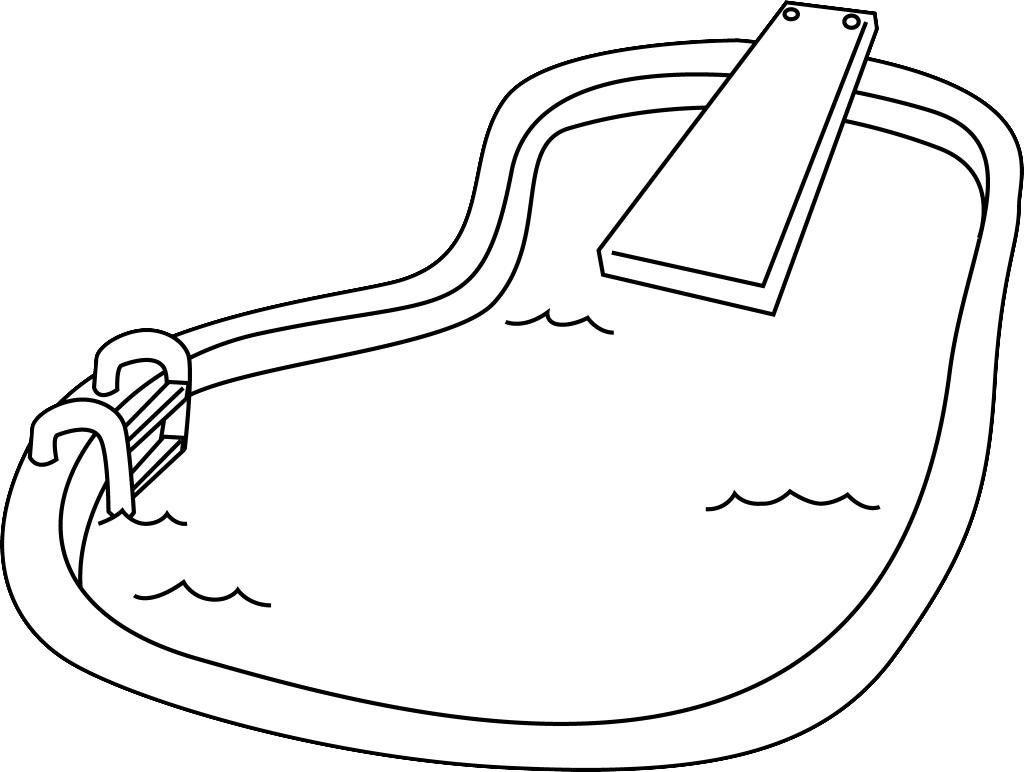
\includegraphics[width=0.4\textwidth]{figs/frontpage/smartpool.png}
\end{minipage}

\vspace{\fill}
\begin{minipage}[l]{\textwidth}
\begin{tabu} to \textwidth{lX[l]}
\textbf{Dato}           &\today\\
\textbf{Vejleder}		&Vejleder navn\\
\end{tabu}
\end{minipage}

\vspace{10pt}
\begin{minipage}[l]{\textwidth}
\tabulinesep=25pt
\begin{tabu} to \textwidth{X[l]X[l]X[l]}
 \makebox[\linewidth]{\hrulefill}\newline Joachim Dam Andersen     \newline 201370248/IKT  
&\makebox[\linewidth]{\hrulefill}\newline Lasse Priebe             \newline 201370248/IKT 
&\makebox[\linewidth]{\hrulefill}\newline Emil Nyborg              \newline 201370248/IKT\\
 \makebox[\linewidth]{\hrulefill}\newline Bjørn Nørgaard Sørensen  \newline 201370248/IKT  
&\makebox[\linewidth]{\hrulefill}\newline Alex Justesen Karlsen    \newline 201370248/IKT 
&\makebox[\linewidth]{\hrulefill}\newline Joachim Händel Noer Wind \newline 201370248/IKT
\end{tabu}
\end{minipage}\clearpage

%% Abstract
% Initial setup
\markboth{RESUMÉ/ABSTRACT}{RESUMÉ/ABSTRACT}
\abstractintoc
\abstractcol
\setlength{\abstitleskip}{-18pt}

% Abstract
\begin{abstract}
Rapporten omhandler et 3. semesterprojekt fra Ingeniørhøjskolen Aarhus Universitet udarbejdet med henblik på at producere et system, som kan fungere som dosering- og sorteringsanlæg til tabletter. Systemet er tiltænkt brug i ældreplejen, som en måde hvorpå fejlmedicinering kan undgås, og tabletsortering kan klares automatisk. Ydermere vil systemet kunne gøre personale og pårørende opmærksomme på, at brugeren ikke har afhentet sine tabletter, indenfor et givet tidsrum. Dette skal formidles ved hjælp af en Android applikation. Systemet og serveren samarbejder om at kontrollerer, hvad der dispenseres til den specifikke bruger og hvornår. Denne kommunikation er ikke fuldt ud implementeret endnu. Systemet var oprindeligt tiltænkt brug i private hjem, men undervejs i processen er idéen ændret idet at fokus flyttes fra private hjem til brug i plejesektoren. 
Produktet kan på nuværende tidspunkt dosere et bestemt antal tabletter af én enkelt type. Systemet har på nuværende tidspunkt allerede implementeret muligheden for at udvide med ekstra dispenserer, og er derfor velegnet til videreudvikling. 
Til systemet er der implementeret en fungerende brugergrænseflade, som er testet med en brugervenlighedsundersøgelse, der ved adspørgelse af 15 studerende har påpeget adskillige muligheder for forbedring.
Under systemudviklingen er den største arbejdsindsats lagt i undersøgelse af teknologier og mulige løsningsforslag.
\end{abstract}

\begin{abstracten}
The report covers a third semesterproject from the Aarhus University School of Engineering. The goal is to produce a system that can function as a dispensing and sorting machine for pills. The system is intended for use in eldercare, as a way of preventing medication errors and a way of sorting pills automaticly. Furthermore, the system will be able to notify staff and relatives if the elder has not picked up their pills, within a given timeperiod. The staff and relatives will be notified via an Android application. The system and a server operate together in order to control what is dispensed to whom and when. Though this communication is not fully implemented yet. The system was originally intended for use in private homes, but during the process, the idea evolved so that the focus was changed from home use to the healthcare sector.
The product can at this time dispense a certain number of pills which will have to be of a single type. The option of adding extra dispensers is already implemented, and is therefore suitable for further development.
The system also has a functioning interface implemented, which has been tested with a user-experience study in which 15 students participated. With the feedback made several things clear, and several of these are suitable for further work.
During the system development the largest effort was put into the study of technologies and potential solutions for the problem chosen.
\end{abstracten}\clearpage

%% Forord
\pagestyle{asereport}
\chapter{Forord}

% Forordet benyttes til at informere kort om visse ydre omstændigheder for projektet, såsom projekttype og hvor projektet er gennemført, historisk baggrund (andre arbejder, som har givet anledning til det aktuelle projekt) og hvor inspirationen og ideen er kommet fra, m.v.

Dette dokument er sammensat for at dokumentere arbejdet på 4. semesterprojektet for retningen IKT på ingeniørhøjskolen Århus.

Der vil i denne rapport være referencer til bilag og dokumentation, som det ikke ville være hensigtsmæssigt at medtage. Samtlige bilag m.m. vil være at finde på den vedlagt CD-rom. 

Source kode til projektet kan findes på CD'en. Link til vores github repo følger her: \newline \url{https://github.com/BjornNorgaard/DuckMaster3001}

\vspace{5mm}

\large{\textit{En stor tak til}}

\begin{displayquote}
    Lars Mortensen for god og brugbar vejledning.
\end{displayquote}

\begin{displayquote}
    Stjerne Apoteket for at lade gruppen komme på besøg og se deres sorteringsmaskine.
\end{displayquote}

\begin{displayquote}
    Sofie Fredslund for at lade os interviewe hende til projektet.
\end{displayquote}

\begin{displayquote}
   Underviserne på ASE, for hjælp og vejledning.
\end{displayquote}

\clearpage

%% ToC
\tableofcontents\clearpage

\mainmatter

%% Todo oversigt - SKAL UDKOMMENTERES FØR AFLEVERING
\listoftodos[Liste over gøremål]

%% Indledning
\chapter{Indledning}

Hello \cite{fysikbog} og sådan kan det jo gå.\clearpage

%% Projektformulering
\documentclass[a4paper,11pt,oneside]{memoir}
\input{utils/packages}
\input{utils/layout}
\input{utils/listings}
\input{utils/ordliste}

%% Forside variabler
\newcommand{\Kursus}{I4PRJ4 F16}
\newcommand{\Projektnavn}{SmartPool 2.0}
\newcommand{\Gruppe}{Gruppe 3}
\newcommand{\Projektdokument}{Projektrapport}

%% Litteratur
\nocite{*}
%\bibliographystyle{harvard}
\bibliography{utils/litteratur}

\begin{document}
\frontmatter

\input{utils/frontpage}\clearpage

%% Abstract
\input{docs/frontmatter/abstract}\clearpage

%% Forord
\pagestyle{asereport}
\input{docs/frontmatter/forord}\clearpage

%% ToC
\tableofcontents\clearpage

\mainmatter

%% Todo oversigt - SKAL UDKOMMENTERES FØR AFLEVERING
\listoftodos[Liste over gøremål]

%% Indledning
\input{docs/frontmatter/indledning}\clearpage

%% Projektformulering
\input{docs/projektformulering/main}\clearpage

%% Kravspecifikation
\input{docs/kravspecifikation/main}\clearpage

%% Systemarkitektur
\input{docs/systemarkitektur/main}\clearpage

%% Processbeskrivelse
\input{docs/processbeskrivelse/main}\clearpage

%% Design
\input{docs/design/main}\clearpage

%% Implementering
\input{docs/implementering/main}\clearpage

%% Integration
\input{docs/integration/main}\clearpage

%% Accepttest
\input{docs/accepttest/main}\clearpage

%% Appendix
\input{docs/appendix/main}\clearpage

\backmatter
%% Glossary
\setglossarystyle{list}
\printnoidxglossary[title=Ordliste]

% Bibliography
\clearpage
\printbibliography[title={Litteratur}]
\end{document}\clearpage

%% Kravspecifikation
\documentclass[a4paper,11pt,oneside]{memoir}
\input{utils/packages}
\input{utils/layout}
\input{utils/listings}
\input{utils/ordliste}

%% Forside variabler
\newcommand{\Kursus}{I4PRJ4 F16}
\newcommand{\Projektnavn}{SmartPool 2.0}
\newcommand{\Gruppe}{Gruppe 3}
\newcommand{\Projektdokument}{Projektrapport}

%% Litteratur
\nocite{*}
%\bibliographystyle{harvard}
\bibliography{utils/litteratur}

\begin{document}
\frontmatter

\input{utils/frontpage}\clearpage

%% Abstract
\input{docs/frontmatter/abstract}\clearpage

%% Forord
\pagestyle{asereport}
\input{docs/frontmatter/forord}\clearpage

%% ToC
\tableofcontents\clearpage

\mainmatter

%% Todo oversigt - SKAL UDKOMMENTERES FØR AFLEVERING
\listoftodos[Liste over gøremål]

%% Indledning
\input{docs/frontmatter/indledning}\clearpage

%% Projektformulering
\input{docs/projektformulering/main}\clearpage

%% Kravspecifikation
\input{docs/kravspecifikation/main}\clearpage

%% Systemarkitektur
\input{docs/systemarkitektur/main}\clearpage

%% Processbeskrivelse
\input{docs/processbeskrivelse/main}\clearpage

%% Design
\input{docs/design/main}\clearpage

%% Implementering
\input{docs/implementering/main}\clearpage

%% Integration
\input{docs/integration/main}\clearpage

%% Accepttest
\input{docs/accepttest/main}\clearpage

%% Appendix
\input{docs/appendix/main}\clearpage

\backmatter
%% Glossary
\setglossarystyle{list}
\printnoidxglossary[title=Ordliste]

% Bibliography
\clearpage
\printbibliography[title={Litteratur}]
\end{document}\clearpage

%% Systemarkitektur
\documentclass[a4paper,11pt,oneside]{memoir}
\input{utils/packages}
\input{utils/layout}
\input{utils/listings}
\input{utils/ordliste}

%% Forside variabler
\newcommand{\Kursus}{I4PRJ4 F16}
\newcommand{\Projektnavn}{SmartPool 2.0}
\newcommand{\Gruppe}{Gruppe 3}
\newcommand{\Projektdokument}{Projektrapport}

%% Litteratur
\nocite{*}
%\bibliographystyle{harvard}
\bibliography{utils/litteratur}

\begin{document}
\frontmatter

\input{utils/frontpage}\clearpage

%% Abstract
\input{docs/frontmatter/abstract}\clearpage

%% Forord
\pagestyle{asereport}
\input{docs/frontmatter/forord}\clearpage

%% ToC
\tableofcontents\clearpage

\mainmatter

%% Todo oversigt - SKAL UDKOMMENTERES FØR AFLEVERING
\listoftodos[Liste over gøremål]

%% Indledning
\input{docs/frontmatter/indledning}\clearpage

%% Projektformulering
\input{docs/projektformulering/main}\clearpage

%% Kravspecifikation
\input{docs/kravspecifikation/main}\clearpage

%% Systemarkitektur
\input{docs/systemarkitektur/main}\clearpage

%% Processbeskrivelse
\input{docs/processbeskrivelse/main}\clearpage

%% Design
\input{docs/design/main}\clearpage

%% Implementering
\input{docs/implementering/main}\clearpage

%% Integration
\input{docs/integration/main}\clearpage

%% Accepttest
\input{docs/accepttest/main}\clearpage

%% Appendix
\input{docs/appendix/main}\clearpage

\backmatter
%% Glossary
\setglossarystyle{list}
\printnoidxglossary[title=Ordliste]

% Bibliography
\clearpage
\printbibliography[title={Litteratur}]
\end{document}\clearpage

%% Processbeskrivelse
\documentclass[a4paper,11pt,oneside]{memoir}
\input{utils/packages}
\input{utils/layout}
\input{utils/listings}
\input{utils/ordliste}

%% Forside variabler
\newcommand{\Kursus}{I4PRJ4 F16}
\newcommand{\Projektnavn}{SmartPool 2.0}
\newcommand{\Gruppe}{Gruppe 3}
\newcommand{\Projektdokument}{Projektrapport}

%% Litteratur
\nocite{*}
%\bibliographystyle{harvard}
\bibliography{utils/litteratur}

\begin{document}
\frontmatter

\input{utils/frontpage}\clearpage

%% Abstract
\input{docs/frontmatter/abstract}\clearpage

%% Forord
\pagestyle{asereport}
\input{docs/frontmatter/forord}\clearpage

%% ToC
\tableofcontents\clearpage

\mainmatter

%% Todo oversigt - SKAL UDKOMMENTERES FØR AFLEVERING
\listoftodos[Liste over gøremål]

%% Indledning
\input{docs/frontmatter/indledning}\clearpage

%% Projektformulering
\input{docs/projektformulering/main}\clearpage

%% Kravspecifikation
\input{docs/kravspecifikation/main}\clearpage

%% Systemarkitektur
\input{docs/systemarkitektur/main}\clearpage

%% Processbeskrivelse
\input{docs/processbeskrivelse/main}\clearpage

%% Design
\input{docs/design/main}\clearpage

%% Implementering
\input{docs/implementering/main}\clearpage

%% Integration
\input{docs/integration/main}\clearpage

%% Accepttest
\input{docs/accepttest/main}\clearpage

%% Appendix
\input{docs/appendix/main}\clearpage

\backmatter
%% Glossary
\setglossarystyle{list}
\printnoidxglossary[title=Ordliste]

% Bibliography
\clearpage
\printbibliography[title={Litteratur}]
\end{document}\clearpage

%% Design
\documentclass[a4paper,11pt,oneside]{memoir}
\input{utils/packages}
\input{utils/layout}
\input{utils/listings}
\input{utils/ordliste}

%% Forside variabler
\newcommand{\Kursus}{I4PRJ4 F16}
\newcommand{\Projektnavn}{SmartPool 2.0}
\newcommand{\Gruppe}{Gruppe 3}
\newcommand{\Projektdokument}{Projektrapport}

%% Litteratur
\nocite{*}
%\bibliographystyle{harvard}
\bibliography{utils/litteratur}

\begin{document}
\frontmatter

\input{utils/frontpage}\clearpage

%% Abstract
\input{docs/frontmatter/abstract}\clearpage

%% Forord
\pagestyle{asereport}
\input{docs/frontmatter/forord}\clearpage

%% ToC
\tableofcontents\clearpage

\mainmatter

%% Todo oversigt - SKAL UDKOMMENTERES FØR AFLEVERING
\listoftodos[Liste over gøremål]

%% Indledning
\input{docs/frontmatter/indledning}\clearpage

%% Projektformulering
\input{docs/projektformulering/main}\clearpage

%% Kravspecifikation
\input{docs/kravspecifikation/main}\clearpage

%% Systemarkitektur
\input{docs/systemarkitektur/main}\clearpage

%% Processbeskrivelse
\input{docs/processbeskrivelse/main}\clearpage

%% Design
\input{docs/design/main}\clearpage

%% Implementering
\input{docs/implementering/main}\clearpage

%% Integration
\input{docs/integration/main}\clearpage

%% Accepttest
\input{docs/accepttest/main}\clearpage

%% Appendix
\input{docs/appendix/main}\clearpage

\backmatter
%% Glossary
\setglossarystyle{list}
\printnoidxglossary[title=Ordliste]

% Bibliography
\clearpage
\printbibliography[title={Litteratur}]
\end{document}\clearpage

%% Implementering
\documentclass[a4paper,11pt,oneside]{memoir}
\input{utils/packages}
\input{utils/layout}
\input{utils/listings}
\input{utils/ordliste}

%% Forside variabler
\newcommand{\Kursus}{I4PRJ4 F16}
\newcommand{\Projektnavn}{SmartPool 2.0}
\newcommand{\Gruppe}{Gruppe 3}
\newcommand{\Projektdokument}{Projektrapport}

%% Litteratur
\nocite{*}
%\bibliographystyle{harvard}
\bibliography{utils/litteratur}

\begin{document}
\frontmatter

\input{utils/frontpage}\clearpage

%% Abstract
\input{docs/frontmatter/abstract}\clearpage

%% Forord
\pagestyle{asereport}
\input{docs/frontmatter/forord}\clearpage

%% ToC
\tableofcontents\clearpage

\mainmatter

%% Todo oversigt - SKAL UDKOMMENTERES FØR AFLEVERING
\listoftodos[Liste over gøremål]

%% Indledning
\input{docs/frontmatter/indledning}\clearpage

%% Projektformulering
\input{docs/projektformulering/main}\clearpage

%% Kravspecifikation
\input{docs/kravspecifikation/main}\clearpage

%% Systemarkitektur
\input{docs/systemarkitektur/main}\clearpage

%% Processbeskrivelse
\input{docs/processbeskrivelse/main}\clearpage

%% Design
\input{docs/design/main}\clearpage

%% Implementering
\input{docs/implementering/main}\clearpage

%% Integration
\input{docs/integration/main}\clearpage

%% Accepttest
\input{docs/accepttest/main}\clearpage

%% Appendix
\input{docs/appendix/main}\clearpage

\backmatter
%% Glossary
\setglossarystyle{list}
\printnoidxglossary[title=Ordliste]

% Bibliography
\clearpage
\printbibliography[title={Litteratur}]
\end{document}\clearpage

%% Integration
\documentclass[a4paper,11pt,oneside]{memoir}
\input{utils/packages}
\input{utils/layout}
\input{utils/listings}
\input{utils/ordliste}

%% Forside variabler
\newcommand{\Kursus}{I4PRJ4 F16}
\newcommand{\Projektnavn}{SmartPool 2.0}
\newcommand{\Gruppe}{Gruppe 3}
\newcommand{\Projektdokument}{Projektrapport}

%% Litteratur
\nocite{*}
%\bibliographystyle{harvard}
\bibliography{utils/litteratur}

\begin{document}
\frontmatter

\input{utils/frontpage}\clearpage

%% Abstract
\input{docs/frontmatter/abstract}\clearpage

%% Forord
\pagestyle{asereport}
\input{docs/frontmatter/forord}\clearpage

%% ToC
\tableofcontents\clearpage

\mainmatter

%% Todo oversigt - SKAL UDKOMMENTERES FØR AFLEVERING
\listoftodos[Liste over gøremål]

%% Indledning
\input{docs/frontmatter/indledning}\clearpage

%% Projektformulering
\input{docs/projektformulering/main}\clearpage

%% Kravspecifikation
\input{docs/kravspecifikation/main}\clearpage

%% Systemarkitektur
\input{docs/systemarkitektur/main}\clearpage

%% Processbeskrivelse
\input{docs/processbeskrivelse/main}\clearpage

%% Design
\input{docs/design/main}\clearpage

%% Implementering
\input{docs/implementering/main}\clearpage

%% Integration
\input{docs/integration/main}\clearpage

%% Accepttest
\input{docs/accepttest/main}\clearpage

%% Appendix
\input{docs/appendix/main}\clearpage

\backmatter
%% Glossary
\setglossarystyle{list}
\printnoidxglossary[title=Ordliste]

% Bibliography
\clearpage
\printbibliography[title={Litteratur}]
\end{document}\clearpage

%% Accepttest
\documentclass[a4paper,11pt,oneside]{memoir}
\input{utils/packages}
\input{utils/layout}
\input{utils/listings}
\input{utils/ordliste}

%% Forside variabler
\newcommand{\Kursus}{I4PRJ4 F16}
\newcommand{\Projektnavn}{SmartPool 2.0}
\newcommand{\Gruppe}{Gruppe 3}
\newcommand{\Projektdokument}{Projektrapport}

%% Litteratur
\nocite{*}
%\bibliographystyle{harvard}
\bibliography{utils/litteratur}

\begin{document}
\frontmatter

\input{utils/frontpage}\clearpage

%% Abstract
\input{docs/frontmatter/abstract}\clearpage

%% Forord
\pagestyle{asereport}
\input{docs/frontmatter/forord}\clearpage

%% ToC
\tableofcontents\clearpage

\mainmatter

%% Todo oversigt - SKAL UDKOMMENTERES FØR AFLEVERING
\listoftodos[Liste over gøremål]

%% Indledning
\input{docs/frontmatter/indledning}\clearpage

%% Projektformulering
\input{docs/projektformulering/main}\clearpage

%% Kravspecifikation
\input{docs/kravspecifikation/main}\clearpage

%% Systemarkitektur
\input{docs/systemarkitektur/main}\clearpage

%% Processbeskrivelse
\input{docs/processbeskrivelse/main}\clearpage

%% Design
\input{docs/design/main}\clearpage

%% Implementering
\input{docs/implementering/main}\clearpage

%% Integration
\input{docs/integration/main}\clearpage

%% Accepttest
\input{docs/accepttest/main}\clearpage

%% Appendix
\input{docs/appendix/main}\clearpage

\backmatter
%% Glossary
\setglossarystyle{list}
\printnoidxglossary[title=Ordliste]

% Bibliography
\clearpage
\printbibliography[title={Litteratur}]
\end{document}\clearpage

%% Appendix
\documentclass[a4paper,11pt,oneside]{memoir}
\input{utils/packages}
\input{utils/layout}
\input{utils/listings}
\input{utils/ordliste}

%% Forside variabler
\newcommand{\Kursus}{I4PRJ4 F16}
\newcommand{\Projektnavn}{SmartPool 2.0}
\newcommand{\Gruppe}{Gruppe 3}
\newcommand{\Projektdokument}{Projektrapport}

%% Litteratur
\nocite{*}
%\bibliographystyle{harvard}
\bibliography{utils/litteratur}

\begin{document}
\frontmatter

\input{utils/frontpage}\clearpage

%% Abstract
\input{docs/frontmatter/abstract}\clearpage

%% Forord
\pagestyle{asereport}
\input{docs/frontmatter/forord}\clearpage

%% ToC
\tableofcontents\clearpage

\mainmatter

%% Todo oversigt - SKAL UDKOMMENTERES FØR AFLEVERING
\listoftodos[Liste over gøremål]

%% Indledning
\input{docs/frontmatter/indledning}\clearpage

%% Projektformulering
\input{docs/projektformulering/main}\clearpage

%% Kravspecifikation
\input{docs/kravspecifikation/main}\clearpage

%% Systemarkitektur
\input{docs/systemarkitektur/main}\clearpage

%% Processbeskrivelse
\input{docs/processbeskrivelse/main}\clearpage

%% Design
\input{docs/design/main}\clearpage

%% Implementering
\input{docs/implementering/main}\clearpage

%% Integration
\input{docs/integration/main}\clearpage

%% Accepttest
\input{docs/accepttest/main}\clearpage

%% Appendix
\input{docs/appendix/main}\clearpage

\backmatter
%% Glossary
\setglossarystyle{list}
\printnoidxglossary[title=Ordliste]

% Bibliography
\clearpage
\printbibliography[title={Litteratur}]
\end{document}\clearpage

\backmatter
%% Glossary
\setglossarystyle{list}
\printnoidxglossary[title=Ordliste]

% Bibliography
\clearpage
\printbibliography[title={Litteratur}]
\end{document}\clearpage

%% Processbeskrivelse
\documentclass[a4paper,11pt,oneside]{memoir}
%!TEX root = main.tex
% Encoding
%\usepackage[utf8]{inputenc} % pdfLatex
\usepackage[T1]{fontenc}
\usepackage[danish]{babel}
\renewcommand{\danishhyphenmins}{22}
\usepackage[utf8]{inputenc} % æ ø å

% Date
\usepackage[ddmmyyyy]{datetime}
\renewcommand{\dateseparator}{.}

% Fonts
\usepackage{fourier}
\usepackage[scaled=0.8]{beramono}

% Math
\usepackage{amsmath,amssymb}
\usepackage{bm}
\usepackage{amsthm}
\usepackage{mathtools}

% Graphics
\usepackage[usenames,dvipsnames,table]{xcolor}
\usepackage{graphicx}
\usepackage{float}
%\usepackage[section]{placeins}
\usepackage{tikz}
\usepackage[pages=some]{background}
\usepackage{wrapfig}

% Listings & Tables
\usepackage{listings}
%\usepackage{pythontex}
\usepackage{enumitem}
\usepackage{tabu}
\usepackage{longtable}
\usepackage{multirow}
\usepackage{makecell}


% References & Quotes
%\usepackage[danish]{varioref}				% Muliggoer bl.a. krydshenvisninger med sidetal (\vref)
%\usepackage{nat}							% Udvidelse med naturvidenskabelige citationsmodeller
\usepackage[danish=guillemets]{csquotes}
\usepackage[hidelinks]{hyperref}
\hypersetup{
    pdfstartview={FitH},
    pdftitle={Smart Pool 2.0},
    pdfsubject={Projektrapport},
    pdfauthor={I4PRJ4GRP3}
}
\usepackage[all]{hypcap}

% Etc
\usepackage[
	%backend=biber,
	backend=bibtex,
	style=ieee,
	natbib=true,
	backref=false,
	backrefstyle=all+,
	hyperref=true
]{biblatex}
\usepackage{pdflscape}
\usepackage[nomain,toc,xindy,acronym,nonumberlist,noredefwarn]{glossaries}
\usepackage[xindy]{imakeidx}
\usepackage{float}
\makeindex

% Dummy
\usepackage{lipsum}
%!TEX root = main.tex
% Page setup
\setulmarginsandblock{35mm}{25mm}{*}
\setlrmarginsandblock{20mm}{20mm}{*}
\setheadfoot{4\onelineskip}{2\onelineskip}
\setheaderspaces{*}{5mm}{*}
\checkandfixthelayout

% Pagestyle
\makepagestyle{asereport}
	\makeevenhead{asereport}{}{}{}
	\makeoddhead{asereport}{
\includegraphics{figs/frontpage/aseaulogo.pdf}}{}{\small\rightmark{} | \textbf{\thepage{}\vspace{7pt}}}
	\makeevenfoot{asereport}{}{}{}
	\makeoddfoot{asereport}{}{}{}

\makepsmarks{asereport}{
	\createmark{chapter}{both}{shownumber}{}{. \ }
	\createmark{section}{both}{shownumber}{}{. \ }
	\createmark{subsection}{both}{shownumber}{}{. \ }
	\createplainmark{toc}{both}{\contentsname}
	\createplainmark{lof}{both}{\listfigurename}
	\createplainmark{lot}{both}{\listtablename}
	\createplainmark{bib}{both}{\bibname}
	\createplainmark{index}{both}{\indexname}
	\createplainmark{glossary}{both}{\glossaryname}
}

\aliaspagestyle{part}{asereport}
\aliaspagestyle{chapter}{asereport}
\chapterstyle{tandh}

% Modification to certain spacing
\setlength{\parskip}{8pt}
\setlength{\parindent}{0pt}
\setlength{\abovecaptionskip}{7pt}
\setlength{\belowcaptionskip}{-10pt}
\OnehalfSpacing

% Tabu
%\taburowcolors[1]2{white .. light-gray}
\tabulinesep=4pt

% Itemize/enumerate
\setlist{
    before=\vspace{-3pt}, 
    after=\vspace{-3pt},
    itemsep=0pt,
    leftmargin=25pt,
    labelsep=10pt,
    topsep=0pt,
}

% Kommandoer til UC - fixer spacing
% Aktører
\newcommand{\fua}[1]{
	\begin{minipage}[t]{\linewidth}
		\setlist{
		    leftmargin=22pt,
		    itemsep=0pt,
		    topsep=0pt,
		    parsep=3pt
		}
	\begin{itemize}[before={\vspace{-6pt}}, after={\vspace{6pt}}]
	#1
	\end{itemize}
	\end{minipage}
}

% Hovedforløb
\newcommand{\fu}[1]{
\begin{minipage}[t]{\linewidth}
\setlist{
    leftmargin=22pt,
    itemsep=0pt,
    topsep=0pt,
    parsep=3pt
}
\raggedright
\begin{enumerate}[before={\vspace{-5pt}},after={\vspace{6pt}}]
#1
\end{enumerate}
\end{minipage}}

% Extensions
\newcommand{\fuex}[2]{
\begin{minipage}[t]{\linewidth}
\vspace{-6pt}
\raggedright
\textit{#1}
\begin{enumerate}[leftmargin=22pt,itemsep=0pt,parsep=3pt,before={\vspace{-8pt}}, after={\vspace{20pt}},topsep=8pt]
#2
\end{enumerate}
\end{minipage}
}

% Extensions - Sidste entry
\newcommand{\fuexl}[2]{
\begin{minipage}[t]{\linewidth}
\vspace{-6pt}
\raggedright
\textit{#1}
\begin{enumerate}[leftmargin=22pt,itemsep=0pt,parsep=3pt,before={\vspace{-8pt}}, after={\vspace{3pt}},topsep=8pt]
#2
\end{enumerate}
\end{minipage}}

% Versionshistorik
\newcommand{\verhistitem}[2]{
\begin{minipage}[t]{\linewidth}
\vspace{-6pt}
\raggedright
#1
\begin{itemize}[leftmargin=22pt,itemsep=0pt,parsep=0pt,before={\vspace{-10pt}},after={\vspace{3pt}},topsep=8pt]
#2
\end{itemize}
\end{minipage}}

\newcommand{\tverb}[1]{{\texttt{#1}}}

\newcommand{\cond}[1]{
\begin{itemize}[label=,noitemsep,topsep=0pt,after={\vspace*{-\baselineskip}}]
#1
\end{itemize}}

% Etc
\definecolor{light-gray}{gray}{0.8}
\definecolor{pantone}{RGB}{0,61,133}

\setfloatlocations{figure}{H}
\setfloatlocations{table}{H}

\numberwithin{equation}{chapter}
\numberwithin{figure}{chapter}
\setcounter{secnumdepth}{3}
\setcounter{tocdepth}{2}
\maxsecnumdepth{subsection}

\renewcommand*{\cftdotsep}{1}
\setpnumwidth{2em}
\setrmarg{2em}

\setverbatimfont{\ttfamily}

%\renewcommand\cftchaptername {\chaptername~}
%\renewcommand\cftappendixname {\appendixname~}
\addto\captionsdanish{
    \renewcommand\contentsname{Indholdsfortegnelse}
    \renewcommand\appendixname{Appendiks}
}
\renewcommand\appendixpagename{Appendiks}
\renewcommand\appendixtocname{Appendiks}
\newsubfloat{figure}

% Abstract
\newenvironment{abstracten}
{\renewcommand{\abstractname}{Abstract}\abstract}
{\endabstract}
\renewcommand{\abstractnamefont}{\normalfont\Large\bfseries}
%!TEX root = main.tex
% Listings
\AtBeginDocument{%
  \counterwithin*{lstlisting}{section}
  \counterwithin*{lstlisting}{subsection}
  \counterwithin*{lstlisting}{subsubsection}
  \renewcommand{\thelstlisting}{%
    \ifnum\value{subsection}=0
      \thesection.\arabic{lstlisting}%
    \else
      \ifnum\value{subsubsection}=0
        \thesubsection.\arabic{lstlisting}%
      \else
        \thesubsubsection.\arabic{lstlisting}%
      \fi
    \fi
  }
}

% Loading languages
\lstloadlanguages{C, C++}

% Listing setup
\lstdefinestyle{all}{
    basicstyle    = \ttfamily\SingleSpacing\scriptsize,
    numbers       = left, 
    numberstyle   = \ttfamily\tiny,
    breaklines    = true,
    commentstyle=\color{green},
    %backgroundcolor = \color{red},
    numbersep     = 20pt,
    xleftmargin   = \parindent,
    captionpos    = b,
    keywordstyle  = [1]\color{Blue}\bfseries,
    commentstyle  = \itshape\color{Green},
    tabsize       = 3
}

\lstset{
    style = all
} 
%!TEX root = main.tex
\makenoidxglossaries
\newglossaryentry{gui}{
    name={GUI}, 
    description={Graphical User Interface er en brugergrænseflade. Brugerens måde at tilgå systemet på}}

\newglossaryentry{psoc}{
    name={PSoC}, 
    description={PSoC (Programmable System-on-Chip) er et microcontroller system produceret af Cypress Semiconductor}}

\newglossaryentry{moscow}{
    name={MoSCoW}, 
    description={MoSCoW er en metode til at prioritere krav til ens system}}

\newglossaryentry{furps}{
    name={FURPS}, 
    description={FURPS er en metode til kategorisering af systemets ikke-funktionelle krav}}

\newglossaryentry{BDD}{
    name={BDD}, 
    description={BDD (Block Definition Diagram) er et diagram, som beskriver et system ved at opdele det op i mindre blokke}}

\newglossaryentry{IBD}{
    name={IBD}, 
    description={IBD (Internal Block Diagram) er et diagram, som viser forbindelserne mellem blokkene, som kan findes i et BDD}}

\newglossaryentry{pilleskuffe}{
    name={Pilleskuffe},
    description={Skuffen under dispenseren, hvor i den nederste pille ligger i. Skuffen tømmes ved at elektromagneten trækker skuffen til sig.}}

\newglossaryentry{pilledispenser}{
    name={Pilledispenser},
    description={Det rør som pillerne bliver opbevaret i.}}

\newglossaryentry{elektromagneten}{
    name={Elektromagneten},
    description={Elektromagneten er en spole der sendes strøm igennem. Når der er strøm på spolen dannes et magnetfelt. Der vil ofte være tale om det samme hvad enten der står spole eller elektromagnet.}}

%% Forside variabler
\newcommand{\Kursus}{I4PRJ4 F16}
\newcommand{\Projektnavn}{SmartPool 2.0}
\newcommand{\Gruppe}{Gruppe 3}
\newcommand{\Projektdokument}{Projektrapport}

%% Litteratur
\nocite{*}
%\bibliographystyle{harvard}
\bibliography{utils/litteratur}

\begin{document}
\frontmatter

%!TEX root = main.tex
\pagestyle{titlingpage}
\backgroundsetup{
	scale=1,
	angle=0,
	opacity=1,
	contents={
		\begin{tikzpicture}[remember picture,overlay]
		\path [fill=pantone] (-0.5\paperwidth,0.36\paperheight) rectangle (0.5\paperwidth,0.47\paperheight);  
		\path [fill=pantone] (-0.5\paperwidth,-0.47\paperheight) rectangle (0.5\paperwidth,-0.43\paperheight);  
		\end{tikzpicture}}}
\BgThispage
\vspace*{-25mm}
\begin{minipage}[l]{\textwidth}
	
\includegraphics[width=0.75\textwidth]{figs/frontpage/aseaulogohvid.pdf}
\end{minipage}

\vspace{35pt}
\begin{minipage}[l]{\textwidth}
\tabulinesep=10pt
\begin{tabu} to \textwidth{X[l]}
	{\small\MakeUppercase\Kursus}\\
	{\HUGE\bfseries\MakeUppercase\Projektnavn}\\
	{\Large\Gruppe}\\
	{\itshape\Projektdokument}
\end{tabu}
\end{minipage}

\vspace{5pt}
\begin{minipage}[l]{\textwidth}
    \centering
	\vspace*{0cm}\hspace*{8cm}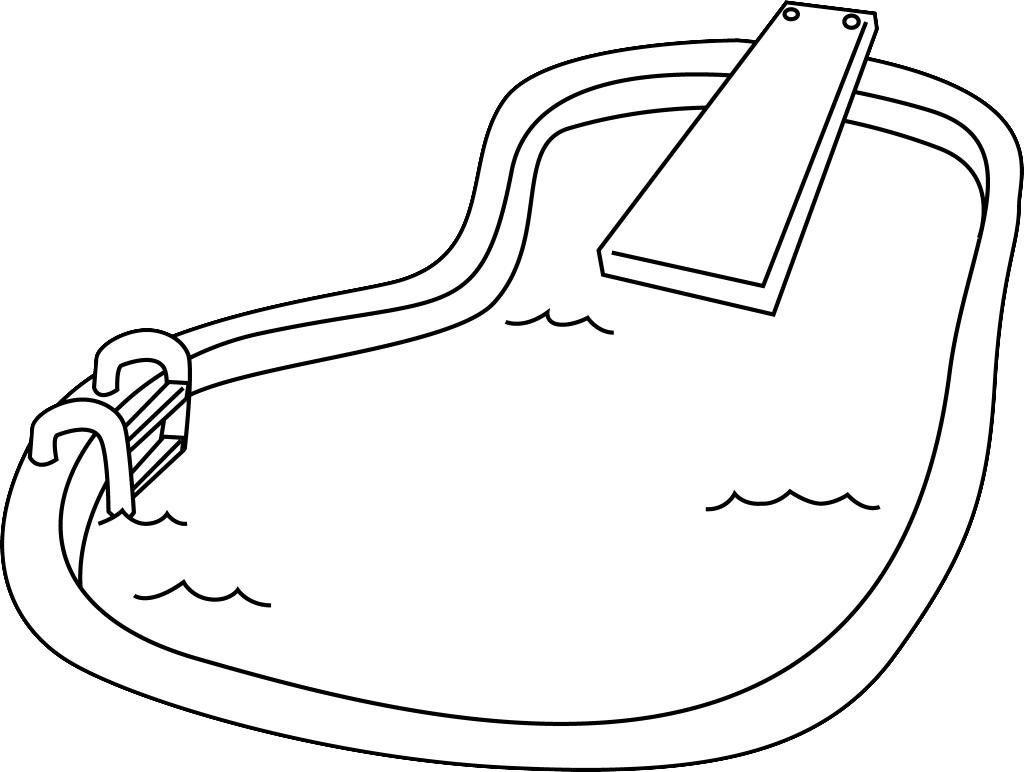
\includegraphics[width=0.4\textwidth]{figs/frontpage/smartpool.png}
\end{minipage}

\vspace{\fill}
\begin{minipage}[l]{\textwidth}
\begin{tabu} to \textwidth{lX[l]}
\textbf{Dato}           &\today\\
\textbf{Vejleder}		&Vejleder navn\\
\end{tabu}
\end{minipage}

\vspace{10pt}
\begin{minipage}[l]{\textwidth}
\tabulinesep=25pt
\begin{tabu} to \textwidth{X[l]X[l]X[l]}
 \makebox[\linewidth]{\hrulefill}\newline Joachim Dam Andersen     \newline 201370248/IKT  
&\makebox[\linewidth]{\hrulefill}\newline Lasse Priebe             \newline 201370248/IKT 
&\makebox[\linewidth]{\hrulefill}\newline Emil Nyborg              \newline 201370248/IKT\\
 \makebox[\linewidth]{\hrulefill}\newline Bjørn Nørgaard Sørensen  \newline 201370248/IKT  
&\makebox[\linewidth]{\hrulefill}\newline Alex Justesen Karlsen    \newline 201370248/IKT 
&\makebox[\linewidth]{\hrulefill}\newline Joachim Händel Noer Wind \newline 201370248/IKT
\end{tabu}
\end{minipage}\clearpage

%% Abstract
% Initial setup
\markboth{RESUMÉ/ABSTRACT}{RESUMÉ/ABSTRACT}
\abstractintoc
\abstractcol
\setlength{\abstitleskip}{-18pt}

% Abstract
\begin{abstract}
Rapporten omhandler et 3. semesterprojekt fra Ingeniørhøjskolen Aarhus Universitet udarbejdet med henblik på at producere et system, som kan fungere som dosering- og sorteringsanlæg til tabletter. Systemet er tiltænkt brug i ældreplejen, som en måde hvorpå fejlmedicinering kan undgås, og tabletsortering kan klares automatisk. Ydermere vil systemet kunne gøre personale og pårørende opmærksomme på, at brugeren ikke har afhentet sine tabletter, indenfor et givet tidsrum. Dette skal formidles ved hjælp af en Android applikation. Systemet og serveren samarbejder om at kontrollerer, hvad der dispenseres til den specifikke bruger og hvornår. Denne kommunikation er ikke fuldt ud implementeret endnu. Systemet var oprindeligt tiltænkt brug i private hjem, men undervejs i processen er idéen ændret idet at fokus flyttes fra private hjem til brug i plejesektoren. 
Produktet kan på nuværende tidspunkt dosere et bestemt antal tabletter af én enkelt type. Systemet har på nuværende tidspunkt allerede implementeret muligheden for at udvide med ekstra dispenserer, og er derfor velegnet til videreudvikling. 
Til systemet er der implementeret en fungerende brugergrænseflade, som er testet med en brugervenlighedsundersøgelse, der ved adspørgelse af 15 studerende har påpeget adskillige muligheder for forbedring.
Under systemudviklingen er den største arbejdsindsats lagt i undersøgelse af teknologier og mulige løsningsforslag.
\end{abstract}

\begin{abstracten}
The report covers a third semesterproject from the Aarhus University School of Engineering. The goal is to produce a system that can function as a dispensing and sorting machine for pills. The system is intended for use in eldercare, as a way of preventing medication errors and a way of sorting pills automaticly. Furthermore, the system will be able to notify staff and relatives if the elder has not picked up their pills, within a given timeperiod. The staff and relatives will be notified via an Android application. The system and a server operate together in order to control what is dispensed to whom and when. Though this communication is not fully implemented yet. The system was originally intended for use in private homes, but during the process, the idea evolved so that the focus was changed from home use to the healthcare sector.
The product can at this time dispense a certain number of pills which will have to be of a single type. The option of adding extra dispensers is already implemented, and is therefore suitable for further development.
The system also has a functioning interface implemented, which has been tested with a user-experience study in which 15 students participated. With the feedback made several things clear, and several of these are suitable for further work.
During the system development the largest effort was put into the study of technologies and potential solutions for the problem chosen.
\end{abstracten}\clearpage

%% Forord
\pagestyle{asereport}
\chapter{Forord}

% Forordet benyttes til at informere kort om visse ydre omstændigheder for projektet, såsom projekttype og hvor projektet er gennemført, historisk baggrund (andre arbejder, som har givet anledning til det aktuelle projekt) og hvor inspirationen og ideen er kommet fra, m.v.

Dette dokument er sammensat for at dokumentere arbejdet på 4. semesterprojektet for retningen IKT på ingeniørhøjskolen Århus.

Der vil i denne rapport være referencer til bilag og dokumentation, som det ikke ville være hensigtsmæssigt at medtage. Samtlige bilag m.m. vil være at finde på den vedlagt CD-rom. 

Source kode til projektet kan findes på CD'en. Link til vores github repo følger her: \newline \url{https://github.com/BjornNorgaard/DuckMaster3001}

\vspace{5mm}

\large{\textit{En stor tak til}}

\begin{displayquote}
    Lars Mortensen for god og brugbar vejledning.
\end{displayquote}

\begin{displayquote}
    Stjerne Apoteket for at lade gruppen komme på besøg og se deres sorteringsmaskine.
\end{displayquote}

\begin{displayquote}
    Sofie Fredslund for at lade os interviewe hende til projektet.
\end{displayquote}

\begin{displayquote}
   Underviserne på ASE, for hjælp og vejledning.
\end{displayquote}

\clearpage

%% ToC
\tableofcontents\clearpage

\mainmatter

%% Todo oversigt - SKAL UDKOMMENTERES FØR AFLEVERING
\listoftodos[Liste over gøremål]

%% Indledning
\chapter{Indledning}

Hello \cite{fysikbog} og sådan kan det jo gå.\clearpage

%% Projektformulering
\documentclass[a4paper,11pt,oneside]{memoir}
\input{utils/packages}
\input{utils/layout}
\input{utils/listings}
\input{utils/ordliste}

%% Forside variabler
\newcommand{\Kursus}{I4PRJ4 F16}
\newcommand{\Projektnavn}{SmartPool 2.0}
\newcommand{\Gruppe}{Gruppe 3}
\newcommand{\Projektdokument}{Projektrapport}

%% Litteratur
\nocite{*}
%\bibliographystyle{harvard}
\bibliography{utils/litteratur}

\begin{document}
\frontmatter

\input{utils/frontpage}\clearpage

%% Abstract
\input{docs/frontmatter/abstract}\clearpage

%% Forord
\pagestyle{asereport}
\input{docs/frontmatter/forord}\clearpage

%% ToC
\tableofcontents\clearpage

\mainmatter

%% Todo oversigt - SKAL UDKOMMENTERES FØR AFLEVERING
\listoftodos[Liste over gøremål]

%% Indledning
\input{docs/frontmatter/indledning}\clearpage

%% Projektformulering
\input{docs/projektformulering/main}\clearpage

%% Kravspecifikation
\input{docs/kravspecifikation/main}\clearpage

%% Systemarkitektur
\input{docs/systemarkitektur/main}\clearpage

%% Processbeskrivelse
\input{docs/processbeskrivelse/main}\clearpage

%% Design
\input{docs/design/main}\clearpage

%% Implementering
\input{docs/implementering/main}\clearpage

%% Integration
\input{docs/integration/main}\clearpage

%% Accepttest
\input{docs/accepttest/main}\clearpage

%% Appendix
\input{docs/appendix/main}\clearpage

\backmatter
%% Glossary
\setglossarystyle{list}
\printnoidxglossary[title=Ordliste]

% Bibliography
\clearpage
\printbibliography[title={Litteratur}]
\end{document}\clearpage

%% Kravspecifikation
\documentclass[a4paper,11pt,oneside]{memoir}
\input{utils/packages}
\input{utils/layout}
\input{utils/listings}
\input{utils/ordliste}

%% Forside variabler
\newcommand{\Kursus}{I4PRJ4 F16}
\newcommand{\Projektnavn}{SmartPool 2.0}
\newcommand{\Gruppe}{Gruppe 3}
\newcommand{\Projektdokument}{Projektrapport}

%% Litteratur
\nocite{*}
%\bibliographystyle{harvard}
\bibliography{utils/litteratur}

\begin{document}
\frontmatter

\input{utils/frontpage}\clearpage

%% Abstract
\input{docs/frontmatter/abstract}\clearpage

%% Forord
\pagestyle{asereport}
\input{docs/frontmatter/forord}\clearpage

%% ToC
\tableofcontents\clearpage

\mainmatter

%% Todo oversigt - SKAL UDKOMMENTERES FØR AFLEVERING
\listoftodos[Liste over gøremål]

%% Indledning
\input{docs/frontmatter/indledning}\clearpage

%% Projektformulering
\input{docs/projektformulering/main}\clearpage

%% Kravspecifikation
\input{docs/kravspecifikation/main}\clearpage

%% Systemarkitektur
\input{docs/systemarkitektur/main}\clearpage

%% Processbeskrivelse
\input{docs/processbeskrivelse/main}\clearpage

%% Design
\input{docs/design/main}\clearpage

%% Implementering
\input{docs/implementering/main}\clearpage

%% Integration
\input{docs/integration/main}\clearpage

%% Accepttest
\input{docs/accepttest/main}\clearpage

%% Appendix
\input{docs/appendix/main}\clearpage

\backmatter
%% Glossary
\setglossarystyle{list}
\printnoidxglossary[title=Ordliste]

% Bibliography
\clearpage
\printbibliography[title={Litteratur}]
\end{document}\clearpage

%% Systemarkitektur
\documentclass[a4paper,11pt,oneside]{memoir}
\input{utils/packages}
\input{utils/layout}
\input{utils/listings}
\input{utils/ordliste}

%% Forside variabler
\newcommand{\Kursus}{I4PRJ4 F16}
\newcommand{\Projektnavn}{SmartPool 2.0}
\newcommand{\Gruppe}{Gruppe 3}
\newcommand{\Projektdokument}{Projektrapport}

%% Litteratur
\nocite{*}
%\bibliographystyle{harvard}
\bibliography{utils/litteratur}

\begin{document}
\frontmatter

\input{utils/frontpage}\clearpage

%% Abstract
\input{docs/frontmatter/abstract}\clearpage

%% Forord
\pagestyle{asereport}
\input{docs/frontmatter/forord}\clearpage

%% ToC
\tableofcontents\clearpage

\mainmatter

%% Todo oversigt - SKAL UDKOMMENTERES FØR AFLEVERING
\listoftodos[Liste over gøremål]

%% Indledning
\input{docs/frontmatter/indledning}\clearpage

%% Projektformulering
\input{docs/projektformulering/main}\clearpage

%% Kravspecifikation
\input{docs/kravspecifikation/main}\clearpage

%% Systemarkitektur
\input{docs/systemarkitektur/main}\clearpage

%% Processbeskrivelse
\input{docs/processbeskrivelse/main}\clearpage

%% Design
\input{docs/design/main}\clearpage

%% Implementering
\input{docs/implementering/main}\clearpage

%% Integration
\input{docs/integration/main}\clearpage

%% Accepttest
\input{docs/accepttest/main}\clearpage

%% Appendix
\input{docs/appendix/main}\clearpage

\backmatter
%% Glossary
\setglossarystyle{list}
\printnoidxglossary[title=Ordliste]

% Bibliography
\clearpage
\printbibliography[title={Litteratur}]
\end{document}\clearpage

%% Processbeskrivelse
\documentclass[a4paper,11pt,oneside]{memoir}
\input{utils/packages}
\input{utils/layout}
\input{utils/listings}
\input{utils/ordliste}

%% Forside variabler
\newcommand{\Kursus}{I4PRJ4 F16}
\newcommand{\Projektnavn}{SmartPool 2.0}
\newcommand{\Gruppe}{Gruppe 3}
\newcommand{\Projektdokument}{Projektrapport}

%% Litteratur
\nocite{*}
%\bibliographystyle{harvard}
\bibliography{utils/litteratur}

\begin{document}
\frontmatter

\input{utils/frontpage}\clearpage

%% Abstract
\input{docs/frontmatter/abstract}\clearpage

%% Forord
\pagestyle{asereport}
\input{docs/frontmatter/forord}\clearpage

%% ToC
\tableofcontents\clearpage

\mainmatter

%% Todo oversigt - SKAL UDKOMMENTERES FØR AFLEVERING
\listoftodos[Liste over gøremål]

%% Indledning
\input{docs/frontmatter/indledning}\clearpage

%% Projektformulering
\input{docs/projektformulering/main}\clearpage

%% Kravspecifikation
\input{docs/kravspecifikation/main}\clearpage

%% Systemarkitektur
\input{docs/systemarkitektur/main}\clearpage

%% Processbeskrivelse
\input{docs/processbeskrivelse/main}\clearpage

%% Design
\input{docs/design/main}\clearpage

%% Implementering
\input{docs/implementering/main}\clearpage

%% Integration
\input{docs/integration/main}\clearpage

%% Accepttest
\input{docs/accepttest/main}\clearpage

%% Appendix
\input{docs/appendix/main}\clearpage

\backmatter
%% Glossary
\setglossarystyle{list}
\printnoidxglossary[title=Ordliste]

% Bibliography
\clearpage
\printbibliography[title={Litteratur}]
\end{document}\clearpage

%% Design
\documentclass[a4paper,11pt,oneside]{memoir}
\input{utils/packages}
\input{utils/layout}
\input{utils/listings}
\input{utils/ordliste}

%% Forside variabler
\newcommand{\Kursus}{I4PRJ4 F16}
\newcommand{\Projektnavn}{SmartPool 2.0}
\newcommand{\Gruppe}{Gruppe 3}
\newcommand{\Projektdokument}{Projektrapport}

%% Litteratur
\nocite{*}
%\bibliographystyle{harvard}
\bibliography{utils/litteratur}

\begin{document}
\frontmatter

\input{utils/frontpage}\clearpage

%% Abstract
\input{docs/frontmatter/abstract}\clearpage

%% Forord
\pagestyle{asereport}
\input{docs/frontmatter/forord}\clearpage

%% ToC
\tableofcontents\clearpage

\mainmatter

%% Todo oversigt - SKAL UDKOMMENTERES FØR AFLEVERING
\listoftodos[Liste over gøremål]

%% Indledning
\input{docs/frontmatter/indledning}\clearpage

%% Projektformulering
\input{docs/projektformulering/main}\clearpage

%% Kravspecifikation
\input{docs/kravspecifikation/main}\clearpage

%% Systemarkitektur
\input{docs/systemarkitektur/main}\clearpage

%% Processbeskrivelse
\input{docs/processbeskrivelse/main}\clearpage

%% Design
\input{docs/design/main}\clearpage

%% Implementering
\input{docs/implementering/main}\clearpage

%% Integration
\input{docs/integration/main}\clearpage

%% Accepttest
\input{docs/accepttest/main}\clearpage

%% Appendix
\input{docs/appendix/main}\clearpage

\backmatter
%% Glossary
\setglossarystyle{list}
\printnoidxglossary[title=Ordliste]

% Bibliography
\clearpage
\printbibliography[title={Litteratur}]
\end{document}\clearpage

%% Implementering
\documentclass[a4paper,11pt,oneside]{memoir}
\input{utils/packages}
\input{utils/layout}
\input{utils/listings}
\input{utils/ordliste}

%% Forside variabler
\newcommand{\Kursus}{I4PRJ4 F16}
\newcommand{\Projektnavn}{SmartPool 2.0}
\newcommand{\Gruppe}{Gruppe 3}
\newcommand{\Projektdokument}{Projektrapport}

%% Litteratur
\nocite{*}
%\bibliographystyle{harvard}
\bibliography{utils/litteratur}

\begin{document}
\frontmatter

\input{utils/frontpage}\clearpage

%% Abstract
\input{docs/frontmatter/abstract}\clearpage

%% Forord
\pagestyle{asereport}
\input{docs/frontmatter/forord}\clearpage

%% ToC
\tableofcontents\clearpage

\mainmatter

%% Todo oversigt - SKAL UDKOMMENTERES FØR AFLEVERING
\listoftodos[Liste over gøremål]

%% Indledning
\input{docs/frontmatter/indledning}\clearpage

%% Projektformulering
\input{docs/projektformulering/main}\clearpage

%% Kravspecifikation
\input{docs/kravspecifikation/main}\clearpage

%% Systemarkitektur
\input{docs/systemarkitektur/main}\clearpage

%% Processbeskrivelse
\input{docs/processbeskrivelse/main}\clearpage

%% Design
\input{docs/design/main}\clearpage

%% Implementering
\input{docs/implementering/main}\clearpage

%% Integration
\input{docs/integration/main}\clearpage

%% Accepttest
\input{docs/accepttest/main}\clearpage

%% Appendix
\input{docs/appendix/main}\clearpage

\backmatter
%% Glossary
\setglossarystyle{list}
\printnoidxglossary[title=Ordliste]

% Bibliography
\clearpage
\printbibliography[title={Litteratur}]
\end{document}\clearpage

%% Integration
\documentclass[a4paper,11pt,oneside]{memoir}
\input{utils/packages}
\input{utils/layout}
\input{utils/listings}
\input{utils/ordliste}

%% Forside variabler
\newcommand{\Kursus}{I4PRJ4 F16}
\newcommand{\Projektnavn}{SmartPool 2.0}
\newcommand{\Gruppe}{Gruppe 3}
\newcommand{\Projektdokument}{Projektrapport}

%% Litteratur
\nocite{*}
%\bibliographystyle{harvard}
\bibliography{utils/litteratur}

\begin{document}
\frontmatter

\input{utils/frontpage}\clearpage

%% Abstract
\input{docs/frontmatter/abstract}\clearpage

%% Forord
\pagestyle{asereport}
\input{docs/frontmatter/forord}\clearpage

%% ToC
\tableofcontents\clearpage

\mainmatter

%% Todo oversigt - SKAL UDKOMMENTERES FØR AFLEVERING
\listoftodos[Liste over gøremål]

%% Indledning
\input{docs/frontmatter/indledning}\clearpage

%% Projektformulering
\input{docs/projektformulering/main}\clearpage

%% Kravspecifikation
\input{docs/kravspecifikation/main}\clearpage

%% Systemarkitektur
\input{docs/systemarkitektur/main}\clearpage

%% Processbeskrivelse
\input{docs/processbeskrivelse/main}\clearpage

%% Design
\input{docs/design/main}\clearpage

%% Implementering
\input{docs/implementering/main}\clearpage

%% Integration
\input{docs/integration/main}\clearpage

%% Accepttest
\input{docs/accepttest/main}\clearpage

%% Appendix
\input{docs/appendix/main}\clearpage

\backmatter
%% Glossary
\setglossarystyle{list}
\printnoidxglossary[title=Ordliste]

% Bibliography
\clearpage
\printbibliography[title={Litteratur}]
\end{document}\clearpage

%% Accepttest
\documentclass[a4paper,11pt,oneside]{memoir}
\input{utils/packages}
\input{utils/layout}
\input{utils/listings}
\input{utils/ordliste}

%% Forside variabler
\newcommand{\Kursus}{I4PRJ4 F16}
\newcommand{\Projektnavn}{SmartPool 2.0}
\newcommand{\Gruppe}{Gruppe 3}
\newcommand{\Projektdokument}{Projektrapport}

%% Litteratur
\nocite{*}
%\bibliographystyle{harvard}
\bibliography{utils/litteratur}

\begin{document}
\frontmatter

\input{utils/frontpage}\clearpage

%% Abstract
\input{docs/frontmatter/abstract}\clearpage

%% Forord
\pagestyle{asereport}
\input{docs/frontmatter/forord}\clearpage

%% ToC
\tableofcontents\clearpage

\mainmatter

%% Todo oversigt - SKAL UDKOMMENTERES FØR AFLEVERING
\listoftodos[Liste over gøremål]

%% Indledning
\input{docs/frontmatter/indledning}\clearpage

%% Projektformulering
\input{docs/projektformulering/main}\clearpage

%% Kravspecifikation
\input{docs/kravspecifikation/main}\clearpage

%% Systemarkitektur
\input{docs/systemarkitektur/main}\clearpage

%% Processbeskrivelse
\input{docs/processbeskrivelse/main}\clearpage

%% Design
\input{docs/design/main}\clearpage

%% Implementering
\input{docs/implementering/main}\clearpage

%% Integration
\input{docs/integration/main}\clearpage

%% Accepttest
\input{docs/accepttest/main}\clearpage

%% Appendix
\input{docs/appendix/main}\clearpage

\backmatter
%% Glossary
\setglossarystyle{list}
\printnoidxglossary[title=Ordliste]

% Bibliography
\clearpage
\printbibliography[title={Litteratur}]
\end{document}\clearpage

%% Appendix
\documentclass[a4paper,11pt,oneside]{memoir}
\input{utils/packages}
\input{utils/layout}
\input{utils/listings}
\input{utils/ordliste}

%% Forside variabler
\newcommand{\Kursus}{I4PRJ4 F16}
\newcommand{\Projektnavn}{SmartPool 2.0}
\newcommand{\Gruppe}{Gruppe 3}
\newcommand{\Projektdokument}{Projektrapport}

%% Litteratur
\nocite{*}
%\bibliographystyle{harvard}
\bibliography{utils/litteratur}

\begin{document}
\frontmatter

\input{utils/frontpage}\clearpage

%% Abstract
\input{docs/frontmatter/abstract}\clearpage

%% Forord
\pagestyle{asereport}
\input{docs/frontmatter/forord}\clearpage

%% ToC
\tableofcontents\clearpage

\mainmatter

%% Todo oversigt - SKAL UDKOMMENTERES FØR AFLEVERING
\listoftodos[Liste over gøremål]

%% Indledning
\input{docs/frontmatter/indledning}\clearpage

%% Projektformulering
\input{docs/projektformulering/main}\clearpage

%% Kravspecifikation
\input{docs/kravspecifikation/main}\clearpage

%% Systemarkitektur
\input{docs/systemarkitektur/main}\clearpage

%% Processbeskrivelse
\input{docs/processbeskrivelse/main}\clearpage

%% Design
\input{docs/design/main}\clearpage

%% Implementering
\input{docs/implementering/main}\clearpage

%% Integration
\input{docs/integration/main}\clearpage

%% Accepttest
\input{docs/accepttest/main}\clearpage

%% Appendix
\input{docs/appendix/main}\clearpage

\backmatter
%% Glossary
\setglossarystyle{list}
\printnoidxglossary[title=Ordliste]

% Bibliography
\clearpage
\printbibliography[title={Litteratur}]
\end{document}\clearpage

\backmatter
%% Glossary
\setglossarystyle{list}
\printnoidxglossary[title=Ordliste]

% Bibliography
\clearpage
\printbibliography[title={Litteratur}]
\end{document}\clearpage

%% Design
\documentclass[a4paper,11pt,oneside]{memoir}
%!TEX root = main.tex
% Encoding
%\usepackage[utf8]{inputenc} % pdfLatex
\usepackage[T1]{fontenc}
\usepackage[danish]{babel}
\renewcommand{\danishhyphenmins}{22}
\usepackage[utf8]{inputenc} % æ ø å

% Date
\usepackage[ddmmyyyy]{datetime}
\renewcommand{\dateseparator}{.}

% Fonts
\usepackage{fourier}
\usepackage[scaled=0.8]{beramono}

% Math
\usepackage{amsmath,amssymb}
\usepackage{bm}
\usepackage{amsthm}
\usepackage{mathtools}

% Graphics
\usepackage[usenames,dvipsnames,table]{xcolor}
\usepackage{graphicx}
\usepackage{float}
%\usepackage[section]{placeins}
\usepackage{tikz}
\usepackage[pages=some]{background}
\usepackage{wrapfig}

% Listings & Tables
\usepackage{listings}
%\usepackage{pythontex}
\usepackage{enumitem}
\usepackage{tabu}
\usepackage{longtable}
\usepackage{multirow}
\usepackage{makecell}


% References & Quotes
%\usepackage[danish]{varioref}				% Muliggoer bl.a. krydshenvisninger med sidetal (\vref)
%\usepackage{nat}							% Udvidelse med naturvidenskabelige citationsmodeller
\usepackage[danish=guillemets]{csquotes}
\usepackage[hidelinks]{hyperref}
\hypersetup{
    pdfstartview={FitH},
    pdftitle={Smart Pool 2.0},
    pdfsubject={Projektrapport},
    pdfauthor={I4PRJ4GRP3}
}
\usepackage[all]{hypcap}

% Etc
\usepackage[
	%backend=biber,
	backend=bibtex,
	style=ieee,
	natbib=true,
	backref=false,
	backrefstyle=all+,
	hyperref=true
]{biblatex}
\usepackage{pdflscape}
\usepackage[nomain,toc,xindy,acronym,nonumberlist,noredefwarn]{glossaries}
\usepackage[xindy]{imakeidx}
\usepackage{float}
\makeindex

% Dummy
\usepackage{lipsum}
%!TEX root = main.tex
% Page setup
\setulmarginsandblock{35mm}{25mm}{*}
\setlrmarginsandblock{20mm}{20mm}{*}
\setheadfoot{4\onelineskip}{2\onelineskip}
\setheaderspaces{*}{5mm}{*}
\checkandfixthelayout

% Pagestyle
\makepagestyle{asereport}
	\makeevenhead{asereport}{}{}{}
	\makeoddhead{asereport}{
\includegraphics{figs/frontpage/aseaulogo.pdf}}{}{\small\rightmark{} | \textbf{\thepage{}\vspace{7pt}}}
	\makeevenfoot{asereport}{}{}{}
	\makeoddfoot{asereport}{}{}{}

\makepsmarks{asereport}{
	\createmark{chapter}{both}{shownumber}{}{. \ }
	\createmark{section}{both}{shownumber}{}{. \ }
	\createmark{subsection}{both}{shownumber}{}{. \ }
	\createplainmark{toc}{both}{\contentsname}
	\createplainmark{lof}{both}{\listfigurename}
	\createplainmark{lot}{both}{\listtablename}
	\createplainmark{bib}{both}{\bibname}
	\createplainmark{index}{both}{\indexname}
	\createplainmark{glossary}{both}{\glossaryname}
}

\aliaspagestyle{part}{asereport}
\aliaspagestyle{chapter}{asereport}
\chapterstyle{tandh}

% Modification to certain spacing
\setlength{\parskip}{8pt}
\setlength{\parindent}{0pt}
\setlength{\abovecaptionskip}{7pt}
\setlength{\belowcaptionskip}{-10pt}
\OnehalfSpacing

% Tabu
%\taburowcolors[1]2{white .. light-gray}
\tabulinesep=4pt

% Itemize/enumerate
\setlist{
    before=\vspace{-3pt}, 
    after=\vspace{-3pt},
    itemsep=0pt,
    leftmargin=25pt,
    labelsep=10pt,
    topsep=0pt,
}

% Kommandoer til UC - fixer spacing
% Aktører
\newcommand{\fua}[1]{
	\begin{minipage}[t]{\linewidth}
		\setlist{
		    leftmargin=22pt,
		    itemsep=0pt,
		    topsep=0pt,
		    parsep=3pt
		}
	\begin{itemize}[before={\vspace{-6pt}}, after={\vspace{6pt}}]
	#1
	\end{itemize}
	\end{minipage}
}

% Hovedforløb
\newcommand{\fu}[1]{
\begin{minipage}[t]{\linewidth}
\setlist{
    leftmargin=22pt,
    itemsep=0pt,
    topsep=0pt,
    parsep=3pt
}
\raggedright
\begin{enumerate}[before={\vspace{-5pt}},after={\vspace{6pt}}]
#1
\end{enumerate}
\end{minipage}}

% Extensions
\newcommand{\fuex}[2]{
\begin{minipage}[t]{\linewidth}
\vspace{-6pt}
\raggedright
\textit{#1}
\begin{enumerate}[leftmargin=22pt,itemsep=0pt,parsep=3pt,before={\vspace{-8pt}}, after={\vspace{20pt}},topsep=8pt]
#2
\end{enumerate}
\end{minipage}
}

% Extensions - Sidste entry
\newcommand{\fuexl}[2]{
\begin{minipage}[t]{\linewidth}
\vspace{-6pt}
\raggedright
\textit{#1}
\begin{enumerate}[leftmargin=22pt,itemsep=0pt,parsep=3pt,before={\vspace{-8pt}}, after={\vspace{3pt}},topsep=8pt]
#2
\end{enumerate}
\end{minipage}}

% Versionshistorik
\newcommand{\verhistitem}[2]{
\begin{minipage}[t]{\linewidth}
\vspace{-6pt}
\raggedright
#1
\begin{itemize}[leftmargin=22pt,itemsep=0pt,parsep=0pt,before={\vspace{-10pt}},after={\vspace{3pt}},topsep=8pt]
#2
\end{itemize}
\end{minipage}}

\newcommand{\tverb}[1]{{\texttt{#1}}}

\newcommand{\cond}[1]{
\begin{itemize}[label=,noitemsep,topsep=0pt,after={\vspace*{-\baselineskip}}]
#1
\end{itemize}}

% Etc
\definecolor{light-gray}{gray}{0.8}
\definecolor{pantone}{RGB}{0,61,133}

\setfloatlocations{figure}{H}
\setfloatlocations{table}{H}

\numberwithin{equation}{chapter}
\numberwithin{figure}{chapter}
\setcounter{secnumdepth}{3}
\setcounter{tocdepth}{2}
\maxsecnumdepth{subsection}

\renewcommand*{\cftdotsep}{1}
\setpnumwidth{2em}
\setrmarg{2em}

\setverbatimfont{\ttfamily}

%\renewcommand\cftchaptername {\chaptername~}
%\renewcommand\cftappendixname {\appendixname~}
\addto\captionsdanish{
    \renewcommand\contentsname{Indholdsfortegnelse}
    \renewcommand\appendixname{Appendiks}
}
\renewcommand\appendixpagename{Appendiks}
\renewcommand\appendixtocname{Appendiks}
\newsubfloat{figure}

% Abstract
\newenvironment{abstracten}
{\renewcommand{\abstractname}{Abstract}\abstract}
{\endabstract}
\renewcommand{\abstractnamefont}{\normalfont\Large\bfseries}
%!TEX root = main.tex
% Listings
\AtBeginDocument{%
  \counterwithin*{lstlisting}{section}
  \counterwithin*{lstlisting}{subsection}
  \counterwithin*{lstlisting}{subsubsection}
  \renewcommand{\thelstlisting}{%
    \ifnum\value{subsection}=0
      \thesection.\arabic{lstlisting}%
    \else
      \ifnum\value{subsubsection}=0
        \thesubsection.\arabic{lstlisting}%
      \else
        \thesubsubsection.\arabic{lstlisting}%
      \fi
    \fi
  }
}

% Loading languages
\lstloadlanguages{C, C++}

% Listing setup
\lstdefinestyle{all}{
    basicstyle    = \ttfamily\SingleSpacing\scriptsize,
    numbers       = left, 
    numberstyle   = \ttfamily\tiny,
    breaklines    = true,
    commentstyle=\color{green},
    %backgroundcolor = \color{red},
    numbersep     = 20pt,
    xleftmargin   = \parindent,
    captionpos    = b,
    keywordstyle  = [1]\color{Blue}\bfseries,
    commentstyle  = \itshape\color{Green},
    tabsize       = 3
}

\lstset{
    style = all
} 
%!TEX root = main.tex
\makenoidxglossaries
\newglossaryentry{gui}{
    name={GUI}, 
    description={Graphical User Interface er en brugergrænseflade. Brugerens måde at tilgå systemet på}}

\newglossaryentry{psoc}{
    name={PSoC}, 
    description={PSoC (Programmable System-on-Chip) er et microcontroller system produceret af Cypress Semiconductor}}

\newglossaryentry{moscow}{
    name={MoSCoW}, 
    description={MoSCoW er en metode til at prioritere krav til ens system}}

\newglossaryentry{furps}{
    name={FURPS}, 
    description={FURPS er en metode til kategorisering af systemets ikke-funktionelle krav}}

\newglossaryentry{BDD}{
    name={BDD}, 
    description={BDD (Block Definition Diagram) er et diagram, som beskriver et system ved at opdele det op i mindre blokke}}

\newglossaryentry{IBD}{
    name={IBD}, 
    description={IBD (Internal Block Diagram) er et diagram, som viser forbindelserne mellem blokkene, som kan findes i et BDD}}

\newglossaryentry{pilleskuffe}{
    name={Pilleskuffe},
    description={Skuffen under dispenseren, hvor i den nederste pille ligger i. Skuffen tømmes ved at elektromagneten trækker skuffen til sig.}}

\newglossaryentry{pilledispenser}{
    name={Pilledispenser},
    description={Det rør som pillerne bliver opbevaret i.}}

\newglossaryentry{elektromagneten}{
    name={Elektromagneten},
    description={Elektromagneten er en spole der sendes strøm igennem. Når der er strøm på spolen dannes et magnetfelt. Der vil ofte være tale om det samme hvad enten der står spole eller elektromagnet.}}

%% Forside variabler
\newcommand{\Kursus}{I4PRJ4 F16}
\newcommand{\Projektnavn}{SmartPool 2.0}
\newcommand{\Gruppe}{Gruppe 3}
\newcommand{\Projektdokument}{Projektrapport}

%% Litteratur
\nocite{*}
%\bibliographystyle{harvard}
\bibliography{utils/litteratur}

\begin{document}
\frontmatter

%!TEX root = main.tex
\pagestyle{titlingpage}
\backgroundsetup{
	scale=1,
	angle=0,
	opacity=1,
	contents={
		\begin{tikzpicture}[remember picture,overlay]
		\path [fill=pantone] (-0.5\paperwidth,0.36\paperheight) rectangle (0.5\paperwidth,0.47\paperheight);  
		\path [fill=pantone] (-0.5\paperwidth,-0.47\paperheight) rectangle (0.5\paperwidth,-0.43\paperheight);  
		\end{tikzpicture}}}
\BgThispage
\vspace*{-25mm}
\begin{minipage}[l]{\textwidth}
	
\includegraphics[width=0.75\textwidth]{figs/frontpage/aseaulogohvid.pdf}
\end{minipage}

\vspace{35pt}
\begin{minipage}[l]{\textwidth}
\tabulinesep=10pt
\begin{tabu} to \textwidth{X[l]}
	{\small\MakeUppercase\Kursus}\\
	{\HUGE\bfseries\MakeUppercase\Projektnavn}\\
	{\Large\Gruppe}\\
	{\itshape\Projektdokument}
\end{tabu}
\end{minipage}

\vspace{5pt}
\begin{minipage}[l]{\textwidth}
    \centering
	\vspace*{0cm}\hspace*{8cm}\includegraphics[width=0.4\textwidth]{figs/frontpage/smartpool.png}
\end{minipage}

\vspace{\fill}
\begin{minipage}[l]{\textwidth}
\begin{tabu} to \textwidth{lX[l]}
\textbf{Dato}           &\today\\
\textbf{Vejleder}		&Vejleder navn\\
\end{tabu}
\end{minipage}

\vspace{10pt}
\begin{minipage}[l]{\textwidth}
\tabulinesep=25pt
\begin{tabu} to \textwidth{X[l]X[l]X[l]}
 \makebox[\linewidth]{\hrulefill}\newline Joachim Dam Andersen     \newline 201370248/IKT  
&\makebox[\linewidth]{\hrulefill}\newline Lasse Priebe             \newline 201370248/IKT 
&\makebox[\linewidth]{\hrulefill}\newline Emil Nyborg              \newline 201370248/IKT\\
 \makebox[\linewidth]{\hrulefill}\newline Bjørn Nørgaard Sørensen  \newline 201370248/IKT  
&\makebox[\linewidth]{\hrulefill}\newline Alex Justesen Karlsen    \newline 201370248/IKT 
&\makebox[\linewidth]{\hrulefill}\newline Joachim Händel Noer Wind \newline 201370248/IKT
\end{tabu}
\end{minipage}\clearpage

%% Abstract
% Initial setup
\markboth{RESUMÉ/ABSTRACT}{RESUMÉ/ABSTRACT}
\abstractintoc
\abstractcol
\setlength{\abstitleskip}{-18pt}

% Abstract
\begin{abstract}
Rapporten omhandler et 3. semesterprojekt fra Ingeniørhøjskolen Aarhus Universitet udarbejdet med henblik på at producere et system, som kan fungere som dosering- og sorteringsanlæg til tabletter. Systemet er tiltænkt brug i ældreplejen, som en måde hvorpå fejlmedicinering kan undgås, og tabletsortering kan klares automatisk. Ydermere vil systemet kunne gøre personale og pårørende opmærksomme på, at brugeren ikke har afhentet sine tabletter, indenfor et givet tidsrum. Dette skal formidles ved hjælp af en Android applikation. Systemet og serveren samarbejder om at kontrollerer, hvad der dispenseres til den specifikke bruger og hvornår. Denne kommunikation er ikke fuldt ud implementeret endnu. Systemet var oprindeligt tiltænkt brug i private hjem, men undervejs i processen er idéen ændret idet at fokus flyttes fra private hjem til brug i plejesektoren. 
Produktet kan på nuværende tidspunkt dosere et bestemt antal tabletter af én enkelt type. Systemet har på nuværende tidspunkt allerede implementeret muligheden for at udvide med ekstra dispenserer, og er derfor velegnet til videreudvikling. 
Til systemet er der implementeret en fungerende brugergrænseflade, som er testet med en brugervenlighedsundersøgelse, der ved adspørgelse af 15 studerende har påpeget adskillige muligheder for forbedring.
Under systemudviklingen er den største arbejdsindsats lagt i undersøgelse af teknologier og mulige løsningsforslag.
\end{abstract}

\begin{abstracten}
The report covers a third semesterproject from the Aarhus University School of Engineering. The goal is to produce a system that can function as a dispensing and sorting machine for pills. The system is intended for use in eldercare, as a way of preventing medication errors and a way of sorting pills automaticly. Furthermore, the system will be able to notify staff and relatives if the elder has not picked up their pills, within a given timeperiod. The staff and relatives will be notified via an Android application. The system and a server operate together in order to control what is dispensed to whom and when. Though this communication is not fully implemented yet. The system was originally intended for use in private homes, but during the process, the idea evolved so that the focus was changed from home use to the healthcare sector.
The product can at this time dispense a certain number of pills which will have to be of a single type. The option of adding extra dispensers is already implemented, and is therefore suitable for further development.
The system also has a functioning interface implemented, which has been tested with a user-experience study in which 15 students participated. With the feedback made several things clear, and several of these are suitable for further work.
During the system development the largest effort was put into the study of technologies and potential solutions for the problem chosen.
\end{abstracten}\clearpage

%% Forord
\pagestyle{asereport}
\chapter{Forord}

% Forordet benyttes til at informere kort om visse ydre omstændigheder for projektet, såsom projekttype og hvor projektet er gennemført, historisk baggrund (andre arbejder, som har givet anledning til det aktuelle projekt) og hvor inspirationen og ideen er kommet fra, m.v.

Dette dokument er sammensat for at dokumentere arbejdet på 4. semesterprojektet for retningen IKT på ingeniørhøjskolen Århus.

Der vil i denne rapport være referencer til bilag og dokumentation, som det ikke ville være hensigtsmæssigt at medtage. Samtlige bilag m.m. vil være at finde på den vedlagt CD-rom. 

Source kode til projektet kan findes på CD'en. Link til vores github repo følger her: \newline \url{https://github.com/BjornNorgaard/DuckMaster3001}

\vspace{5mm}

\large{\textit{En stor tak til}}

\begin{displayquote}
    Lars Mortensen for god og brugbar vejledning.
\end{displayquote}

\begin{displayquote}
    Stjerne Apoteket for at lade gruppen komme på besøg og se deres sorteringsmaskine.
\end{displayquote}

\begin{displayquote}
    Sofie Fredslund for at lade os interviewe hende til projektet.
\end{displayquote}

\begin{displayquote}
   Underviserne på ASE, for hjælp og vejledning.
\end{displayquote}

\clearpage

%% ToC
\tableofcontents\clearpage

\mainmatter

%% Todo oversigt - SKAL UDKOMMENTERES FØR AFLEVERING
\listoftodos[Liste over gøremål]

%% Indledning
\chapter{Indledning}

Hello \cite{fysikbog} og sådan kan det jo gå.\clearpage

%% Projektformulering
\documentclass[a4paper,11pt,oneside]{memoir}
\input{utils/packages}
\input{utils/layout}
\input{utils/listings}
\input{utils/ordliste}

%% Forside variabler
\newcommand{\Kursus}{I4PRJ4 F16}
\newcommand{\Projektnavn}{SmartPool 2.0}
\newcommand{\Gruppe}{Gruppe 3}
\newcommand{\Projektdokument}{Projektrapport}

%% Litteratur
\nocite{*}
%\bibliographystyle{harvard}
\bibliography{utils/litteratur}

\begin{document}
\frontmatter

\input{utils/frontpage}\clearpage

%% Abstract
\input{docs/frontmatter/abstract}\clearpage

%% Forord
\pagestyle{asereport}
\input{docs/frontmatter/forord}\clearpage

%% ToC
\tableofcontents\clearpage

\mainmatter

%% Todo oversigt - SKAL UDKOMMENTERES FØR AFLEVERING
\listoftodos[Liste over gøremål]

%% Indledning
\input{docs/frontmatter/indledning}\clearpage

%% Projektformulering
\input{docs/projektformulering/main}\clearpage

%% Kravspecifikation
\input{docs/kravspecifikation/main}\clearpage

%% Systemarkitektur
\input{docs/systemarkitektur/main}\clearpage

%% Processbeskrivelse
\input{docs/processbeskrivelse/main}\clearpage

%% Design
\input{docs/design/main}\clearpage

%% Implementering
\input{docs/implementering/main}\clearpage

%% Integration
\input{docs/integration/main}\clearpage

%% Accepttest
\input{docs/accepttest/main}\clearpage

%% Appendix
\input{docs/appendix/main}\clearpage

\backmatter
%% Glossary
\setglossarystyle{list}
\printnoidxglossary[title=Ordliste]

% Bibliography
\clearpage
\printbibliography[title={Litteratur}]
\end{document}\clearpage

%% Kravspecifikation
\documentclass[a4paper,11pt,oneside]{memoir}
\input{utils/packages}
\input{utils/layout}
\input{utils/listings}
\input{utils/ordliste}

%% Forside variabler
\newcommand{\Kursus}{I4PRJ4 F16}
\newcommand{\Projektnavn}{SmartPool 2.0}
\newcommand{\Gruppe}{Gruppe 3}
\newcommand{\Projektdokument}{Projektrapport}

%% Litteratur
\nocite{*}
%\bibliographystyle{harvard}
\bibliography{utils/litteratur}

\begin{document}
\frontmatter

\input{utils/frontpage}\clearpage

%% Abstract
\input{docs/frontmatter/abstract}\clearpage

%% Forord
\pagestyle{asereport}
\input{docs/frontmatter/forord}\clearpage

%% ToC
\tableofcontents\clearpage

\mainmatter

%% Todo oversigt - SKAL UDKOMMENTERES FØR AFLEVERING
\listoftodos[Liste over gøremål]

%% Indledning
\input{docs/frontmatter/indledning}\clearpage

%% Projektformulering
\input{docs/projektformulering/main}\clearpage

%% Kravspecifikation
\input{docs/kravspecifikation/main}\clearpage

%% Systemarkitektur
\input{docs/systemarkitektur/main}\clearpage

%% Processbeskrivelse
\input{docs/processbeskrivelse/main}\clearpage

%% Design
\input{docs/design/main}\clearpage

%% Implementering
\input{docs/implementering/main}\clearpage

%% Integration
\input{docs/integration/main}\clearpage

%% Accepttest
\input{docs/accepttest/main}\clearpage

%% Appendix
\input{docs/appendix/main}\clearpage

\backmatter
%% Glossary
\setglossarystyle{list}
\printnoidxglossary[title=Ordliste]

% Bibliography
\clearpage
\printbibliography[title={Litteratur}]
\end{document}\clearpage

%% Systemarkitektur
\documentclass[a4paper,11pt,oneside]{memoir}
\input{utils/packages}
\input{utils/layout}
\input{utils/listings}
\input{utils/ordliste}

%% Forside variabler
\newcommand{\Kursus}{I4PRJ4 F16}
\newcommand{\Projektnavn}{SmartPool 2.0}
\newcommand{\Gruppe}{Gruppe 3}
\newcommand{\Projektdokument}{Projektrapport}

%% Litteratur
\nocite{*}
%\bibliographystyle{harvard}
\bibliography{utils/litteratur}

\begin{document}
\frontmatter

\input{utils/frontpage}\clearpage

%% Abstract
\input{docs/frontmatter/abstract}\clearpage

%% Forord
\pagestyle{asereport}
\input{docs/frontmatter/forord}\clearpage

%% ToC
\tableofcontents\clearpage

\mainmatter

%% Todo oversigt - SKAL UDKOMMENTERES FØR AFLEVERING
\listoftodos[Liste over gøremål]

%% Indledning
\input{docs/frontmatter/indledning}\clearpage

%% Projektformulering
\input{docs/projektformulering/main}\clearpage

%% Kravspecifikation
\input{docs/kravspecifikation/main}\clearpage

%% Systemarkitektur
\input{docs/systemarkitektur/main}\clearpage

%% Processbeskrivelse
\input{docs/processbeskrivelse/main}\clearpage

%% Design
\input{docs/design/main}\clearpage

%% Implementering
\input{docs/implementering/main}\clearpage

%% Integration
\input{docs/integration/main}\clearpage

%% Accepttest
\input{docs/accepttest/main}\clearpage

%% Appendix
\input{docs/appendix/main}\clearpage

\backmatter
%% Glossary
\setglossarystyle{list}
\printnoidxglossary[title=Ordliste]

% Bibliography
\clearpage
\printbibliography[title={Litteratur}]
\end{document}\clearpage

%% Processbeskrivelse
\documentclass[a4paper,11pt,oneside]{memoir}
\input{utils/packages}
\input{utils/layout}
\input{utils/listings}
\input{utils/ordliste}

%% Forside variabler
\newcommand{\Kursus}{I4PRJ4 F16}
\newcommand{\Projektnavn}{SmartPool 2.0}
\newcommand{\Gruppe}{Gruppe 3}
\newcommand{\Projektdokument}{Projektrapport}

%% Litteratur
\nocite{*}
%\bibliographystyle{harvard}
\bibliography{utils/litteratur}

\begin{document}
\frontmatter

\input{utils/frontpage}\clearpage

%% Abstract
\input{docs/frontmatter/abstract}\clearpage

%% Forord
\pagestyle{asereport}
\input{docs/frontmatter/forord}\clearpage

%% ToC
\tableofcontents\clearpage

\mainmatter

%% Todo oversigt - SKAL UDKOMMENTERES FØR AFLEVERING
\listoftodos[Liste over gøremål]

%% Indledning
\input{docs/frontmatter/indledning}\clearpage

%% Projektformulering
\input{docs/projektformulering/main}\clearpage

%% Kravspecifikation
\input{docs/kravspecifikation/main}\clearpage

%% Systemarkitektur
\input{docs/systemarkitektur/main}\clearpage

%% Processbeskrivelse
\input{docs/processbeskrivelse/main}\clearpage

%% Design
\input{docs/design/main}\clearpage

%% Implementering
\input{docs/implementering/main}\clearpage

%% Integration
\input{docs/integration/main}\clearpage

%% Accepttest
\input{docs/accepttest/main}\clearpage

%% Appendix
\input{docs/appendix/main}\clearpage

\backmatter
%% Glossary
\setglossarystyle{list}
\printnoidxglossary[title=Ordliste]

% Bibliography
\clearpage
\printbibliography[title={Litteratur}]
\end{document}\clearpage

%% Design
\documentclass[a4paper,11pt,oneside]{memoir}
\input{utils/packages}
\input{utils/layout}
\input{utils/listings}
\input{utils/ordliste}

%% Forside variabler
\newcommand{\Kursus}{I4PRJ4 F16}
\newcommand{\Projektnavn}{SmartPool 2.0}
\newcommand{\Gruppe}{Gruppe 3}
\newcommand{\Projektdokument}{Projektrapport}

%% Litteratur
\nocite{*}
%\bibliographystyle{harvard}
\bibliography{utils/litteratur}

\begin{document}
\frontmatter

\input{utils/frontpage}\clearpage

%% Abstract
\input{docs/frontmatter/abstract}\clearpage

%% Forord
\pagestyle{asereport}
\input{docs/frontmatter/forord}\clearpage

%% ToC
\tableofcontents\clearpage

\mainmatter

%% Todo oversigt - SKAL UDKOMMENTERES FØR AFLEVERING
\listoftodos[Liste over gøremål]

%% Indledning
\input{docs/frontmatter/indledning}\clearpage

%% Projektformulering
\input{docs/projektformulering/main}\clearpage

%% Kravspecifikation
\input{docs/kravspecifikation/main}\clearpage

%% Systemarkitektur
\input{docs/systemarkitektur/main}\clearpage

%% Processbeskrivelse
\input{docs/processbeskrivelse/main}\clearpage

%% Design
\input{docs/design/main}\clearpage

%% Implementering
\input{docs/implementering/main}\clearpage

%% Integration
\input{docs/integration/main}\clearpage

%% Accepttest
\input{docs/accepttest/main}\clearpage

%% Appendix
\input{docs/appendix/main}\clearpage

\backmatter
%% Glossary
\setglossarystyle{list}
\printnoidxglossary[title=Ordliste]

% Bibliography
\clearpage
\printbibliography[title={Litteratur}]
\end{document}\clearpage

%% Implementering
\documentclass[a4paper,11pt,oneside]{memoir}
\input{utils/packages}
\input{utils/layout}
\input{utils/listings}
\input{utils/ordliste}

%% Forside variabler
\newcommand{\Kursus}{I4PRJ4 F16}
\newcommand{\Projektnavn}{SmartPool 2.0}
\newcommand{\Gruppe}{Gruppe 3}
\newcommand{\Projektdokument}{Projektrapport}

%% Litteratur
\nocite{*}
%\bibliographystyle{harvard}
\bibliography{utils/litteratur}

\begin{document}
\frontmatter

\input{utils/frontpage}\clearpage

%% Abstract
\input{docs/frontmatter/abstract}\clearpage

%% Forord
\pagestyle{asereport}
\input{docs/frontmatter/forord}\clearpage

%% ToC
\tableofcontents\clearpage

\mainmatter

%% Todo oversigt - SKAL UDKOMMENTERES FØR AFLEVERING
\listoftodos[Liste over gøremål]

%% Indledning
\input{docs/frontmatter/indledning}\clearpage

%% Projektformulering
\input{docs/projektformulering/main}\clearpage

%% Kravspecifikation
\input{docs/kravspecifikation/main}\clearpage

%% Systemarkitektur
\input{docs/systemarkitektur/main}\clearpage

%% Processbeskrivelse
\input{docs/processbeskrivelse/main}\clearpage

%% Design
\input{docs/design/main}\clearpage

%% Implementering
\input{docs/implementering/main}\clearpage

%% Integration
\input{docs/integration/main}\clearpage

%% Accepttest
\input{docs/accepttest/main}\clearpage

%% Appendix
\input{docs/appendix/main}\clearpage

\backmatter
%% Glossary
\setglossarystyle{list}
\printnoidxglossary[title=Ordliste]

% Bibliography
\clearpage
\printbibliography[title={Litteratur}]
\end{document}\clearpage

%% Integration
\documentclass[a4paper,11pt,oneside]{memoir}
\input{utils/packages}
\input{utils/layout}
\input{utils/listings}
\input{utils/ordliste}

%% Forside variabler
\newcommand{\Kursus}{I4PRJ4 F16}
\newcommand{\Projektnavn}{SmartPool 2.0}
\newcommand{\Gruppe}{Gruppe 3}
\newcommand{\Projektdokument}{Projektrapport}

%% Litteratur
\nocite{*}
%\bibliographystyle{harvard}
\bibliography{utils/litteratur}

\begin{document}
\frontmatter

\input{utils/frontpage}\clearpage

%% Abstract
\input{docs/frontmatter/abstract}\clearpage

%% Forord
\pagestyle{asereport}
\input{docs/frontmatter/forord}\clearpage

%% ToC
\tableofcontents\clearpage

\mainmatter

%% Todo oversigt - SKAL UDKOMMENTERES FØR AFLEVERING
\listoftodos[Liste over gøremål]

%% Indledning
\input{docs/frontmatter/indledning}\clearpage

%% Projektformulering
\input{docs/projektformulering/main}\clearpage

%% Kravspecifikation
\input{docs/kravspecifikation/main}\clearpage

%% Systemarkitektur
\input{docs/systemarkitektur/main}\clearpage

%% Processbeskrivelse
\input{docs/processbeskrivelse/main}\clearpage

%% Design
\input{docs/design/main}\clearpage

%% Implementering
\input{docs/implementering/main}\clearpage

%% Integration
\input{docs/integration/main}\clearpage

%% Accepttest
\input{docs/accepttest/main}\clearpage

%% Appendix
\input{docs/appendix/main}\clearpage

\backmatter
%% Glossary
\setglossarystyle{list}
\printnoidxglossary[title=Ordliste]

% Bibliography
\clearpage
\printbibliography[title={Litteratur}]
\end{document}\clearpage

%% Accepttest
\documentclass[a4paper,11pt,oneside]{memoir}
\input{utils/packages}
\input{utils/layout}
\input{utils/listings}
\input{utils/ordliste}

%% Forside variabler
\newcommand{\Kursus}{I4PRJ4 F16}
\newcommand{\Projektnavn}{SmartPool 2.0}
\newcommand{\Gruppe}{Gruppe 3}
\newcommand{\Projektdokument}{Projektrapport}

%% Litteratur
\nocite{*}
%\bibliographystyle{harvard}
\bibliography{utils/litteratur}

\begin{document}
\frontmatter

\input{utils/frontpage}\clearpage

%% Abstract
\input{docs/frontmatter/abstract}\clearpage

%% Forord
\pagestyle{asereport}
\input{docs/frontmatter/forord}\clearpage

%% ToC
\tableofcontents\clearpage

\mainmatter

%% Todo oversigt - SKAL UDKOMMENTERES FØR AFLEVERING
\listoftodos[Liste over gøremål]

%% Indledning
\input{docs/frontmatter/indledning}\clearpage

%% Projektformulering
\input{docs/projektformulering/main}\clearpage

%% Kravspecifikation
\input{docs/kravspecifikation/main}\clearpage

%% Systemarkitektur
\input{docs/systemarkitektur/main}\clearpage

%% Processbeskrivelse
\input{docs/processbeskrivelse/main}\clearpage

%% Design
\input{docs/design/main}\clearpage

%% Implementering
\input{docs/implementering/main}\clearpage

%% Integration
\input{docs/integration/main}\clearpage

%% Accepttest
\input{docs/accepttest/main}\clearpage

%% Appendix
\input{docs/appendix/main}\clearpage

\backmatter
%% Glossary
\setglossarystyle{list}
\printnoidxglossary[title=Ordliste]

% Bibliography
\clearpage
\printbibliography[title={Litteratur}]
\end{document}\clearpage

%% Appendix
\documentclass[a4paper,11pt,oneside]{memoir}
\input{utils/packages}
\input{utils/layout}
\input{utils/listings}
\input{utils/ordliste}

%% Forside variabler
\newcommand{\Kursus}{I4PRJ4 F16}
\newcommand{\Projektnavn}{SmartPool 2.0}
\newcommand{\Gruppe}{Gruppe 3}
\newcommand{\Projektdokument}{Projektrapport}

%% Litteratur
\nocite{*}
%\bibliographystyle{harvard}
\bibliography{utils/litteratur}

\begin{document}
\frontmatter

\input{utils/frontpage}\clearpage

%% Abstract
\input{docs/frontmatter/abstract}\clearpage

%% Forord
\pagestyle{asereport}
\input{docs/frontmatter/forord}\clearpage

%% ToC
\tableofcontents\clearpage

\mainmatter

%% Todo oversigt - SKAL UDKOMMENTERES FØR AFLEVERING
\listoftodos[Liste over gøremål]

%% Indledning
\input{docs/frontmatter/indledning}\clearpage

%% Projektformulering
\input{docs/projektformulering/main}\clearpage

%% Kravspecifikation
\input{docs/kravspecifikation/main}\clearpage

%% Systemarkitektur
\input{docs/systemarkitektur/main}\clearpage

%% Processbeskrivelse
\input{docs/processbeskrivelse/main}\clearpage

%% Design
\input{docs/design/main}\clearpage

%% Implementering
\input{docs/implementering/main}\clearpage

%% Integration
\input{docs/integration/main}\clearpage

%% Accepttest
\input{docs/accepttest/main}\clearpage

%% Appendix
\input{docs/appendix/main}\clearpage

\backmatter
%% Glossary
\setglossarystyle{list}
\printnoidxglossary[title=Ordliste]

% Bibliography
\clearpage
\printbibliography[title={Litteratur}]
\end{document}\clearpage

\backmatter
%% Glossary
\setglossarystyle{list}
\printnoidxglossary[title=Ordliste]

% Bibliography
\clearpage
\printbibliography[title={Litteratur}]
\end{document}\clearpage

%% Implementering
\documentclass[a4paper,11pt,oneside]{memoir}
%!TEX root = main.tex
% Encoding
%\usepackage[utf8]{inputenc} % pdfLatex
\usepackage[T1]{fontenc}
\usepackage[danish]{babel}
\renewcommand{\danishhyphenmins}{22}
\usepackage[utf8]{inputenc} % æ ø å

% Date
\usepackage[ddmmyyyy]{datetime}
\renewcommand{\dateseparator}{.}

% Fonts
\usepackage{fourier}
\usepackage[scaled=0.8]{beramono}

% Math
\usepackage{amsmath,amssymb}
\usepackage{bm}
\usepackage{amsthm}
\usepackage{mathtools}

% Graphics
\usepackage[usenames,dvipsnames,table]{xcolor}
\usepackage{graphicx}
\usepackage{float}
%\usepackage[section]{placeins}
\usepackage{tikz}
\usepackage[pages=some]{background}
\usepackage{wrapfig}

% Listings & Tables
\usepackage{listings}
%\usepackage{pythontex}
\usepackage{enumitem}
\usepackage{tabu}
\usepackage{longtable}
\usepackage{multirow}
\usepackage{makecell}


% References & Quotes
%\usepackage[danish]{varioref}				% Muliggoer bl.a. krydshenvisninger med sidetal (\vref)
%\usepackage{nat}							% Udvidelse med naturvidenskabelige citationsmodeller
\usepackage[danish=guillemets]{csquotes}
\usepackage[hidelinks]{hyperref}
\hypersetup{
    pdfstartview={FitH},
    pdftitle={Smart Pool 2.0},
    pdfsubject={Projektrapport},
    pdfauthor={I4PRJ4GRP3}
}
\usepackage[all]{hypcap}

% Etc
\usepackage[
	%backend=biber,
	backend=bibtex,
	style=ieee,
	natbib=true,
	backref=false,
	backrefstyle=all+,
	hyperref=true
]{biblatex}
\usepackage{pdflscape}
\usepackage[nomain,toc,xindy,acronym,nonumberlist,noredefwarn]{glossaries}
\usepackage[xindy]{imakeidx}
\usepackage{float}
\makeindex

% Dummy
\usepackage{lipsum}
%!TEX root = main.tex
% Page setup
\setulmarginsandblock{35mm}{25mm}{*}
\setlrmarginsandblock{20mm}{20mm}{*}
\setheadfoot{4\onelineskip}{2\onelineskip}
\setheaderspaces{*}{5mm}{*}
\checkandfixthelayout

% Pagestyle
\makepagestyle{asereport}
	\makeevenhead{asereport}{}{}{}
	\makeoddhead{asereport}{\includegraphics{figs/frontpage/aseaulogo.pdf}}{}{\small\rightmark{} | \textbf{\thepage{}\vspace{7pt}}}
	\makeevenfoot{asereport}{}{}{}
	\makeoddfoot{asereport}{}{}{}

\makepsmarks{asereport}{
	\createmark{chapter}{both}{shownumber}{}{. \ }
	\createmark{section}{both}{shownumber}{}{. \ }
	\createmark{subsection}{both}{shownumber}{}{. \ }
	\createplainmark{toc}{both}{\contentsname}
	\createplainmark{lof}{both}{\listfigurename}
	\createplainmark{lot}{both}{\listtablename}
	\createplainmark{bib}{both}{\bibname}
	\createplainmark{index}{both}{\indexname}
	\createplainmark{glossary}{both}{\glossaryname}
}

\aliaspagestyle{part}{asereport}
\aliaspagestyle{chapter}{asereport}
\chapterstyle{tandh}

% Modification to certain spacing
\setlength{\parskip}{8pt}
\setlength{\parindent}{0pt}
\setlength{\abovecaptionskip}{7pt}
\setlength{\belowcaptionskip}{-10pt}
\OnehalfSpacing

% Tabu
%\taburowcolors[1]2{white .. light-gray}
\tabulinesep=4pt

% Itemize/enumerate
\setlist{
    before=\vspace{-3pt}, 
    after=\vspace{-3pt},
    itemsep=0pt,
    leftmargin=25pt,
    labelsep=10pt,
    topsep=0pt,
}

% Kommandoer til UC - fixer spacing
% Aktører
\newcommand{\fua}[1]{
	\begin{minipage}[t]{\linewidth}
		\setlist{
		    leftmargin=22pt,
		    itemsep=0pt,
		    topsep=0pt,
		    parsep=3pt
		}
	\begin{itemize}[before={\vspace{-6pt}}, after={\vspace{6pt}}]
	#1
	\end{itemize}
	\end{minipage}
}

% Hovedforløb
\newcommand{\fu}[1]{
\begin{minipage}[t]{\linewidth}
\setlist{
    leftmargin=22pt,
    itemsep=0pt,
    topsep=0pt,
    parsep=3pt
}
\raggedright
\begin{enumerate}[before={\vspace{-5pt}},after={\vspace{6pt}}]
#1
\end{enumerate}
\end{minipage}}

% Extensions
\newcommand{\fuex}[2]{
\begin{minipage}[t]{\linewidth}
\vspace{-6pt}
\raggedright
\textit{#1}
\begin{enumerate}[leftmargin=22pt,itemsep=0pt,parsep=3pt,before={\vspace{-8pt}}, after={\vspace{20pt}},topsep=8pt]
#2
\end{enumerate}
\end{minipage}
}

% Extensions - Sidste entry
\newcommand{\fuexl}[2]{
\begin{minipage}[t]{\linewidth}
\vspace{-6pt}
\raggedright
\textit{#1}
\begin{enumerate}[leftmargin=22pt,itemsep=0pt,parsep=3pt,before={\vspace{-8pt}}, after={\vspace{3pt}},topsep=8pt]
#2
\end{enumerate}
\end{minipage}}

% Versionshistorik
\newcommand{\verhistitem}[2]{
\begin{minipage}[t]{\linewidth}
\vspace{-6pt}
\raggedright
#1
\begin{itemize}[leftmargin=22pt,itemsep=0pt,parsep=0pt,before={\vspace{-10pt}},after={\vspace{3pt}},topsep=8pt]
#2
\end{itemize}
\end{minipage}}

\newcommand{\tverb}[1]{{\texttt{#1}}}

\newcommand{\cond}[1]{
\begin{itemize}[label=,noitemsep,topsep=0pt,after={\vspace*{-\baselineskip}}]
#1
\end{itemize}}

% Etc
\definecolor{light-gray}{gray}{0.8}
\definecolor{pantone}{RGB}{0,61,133}

\setfloatlocations{figure}{H}
\setfloatlocations{table}{H}

\numberwithin{equation}{chapter}
\numberwithin{figure}{chapter}
\setcounter{secnumdepth}{3}
\setcounter{tocdepth}{2}
\maxsecnumdepth{subsection}

\renewcommand*{\cftdotsep}{1}
\setpnumwidth{2em}
\setrmarg{2em}

\setverbatimfont{\ttfamily}

%\renewcommand\cftchaptername {\chaptername~}
%\renewcommand\cftappendixname {\appendixname~}
\addto\captionsdanish{
    \renewcommand\contentsname{Indholdsfortegnelse}
    \renewcommand\appendixname{Appendiks}
}
\renewcommand\appendixpagename{Appendiks}
\renewcommand\appendixtocname{Appendiks}
\newsubfloat{figure}

% Abstract
\newenvironment{abstracten}
{\renewcommand{\abstractname}{Abstract}\abstract}
{\endabstract}
\renewcommand{\abstractnamefont}{\normalfont\Large\bfseries}
%!TEX root = main.tex
% Listings
\AtBeginDocument{%
  \counterwithin*{lstlisting}{section}
  \counterwithin*{lstlisting}{subsection}
  \counterwithin*{lstlisting}{subsubsection}
  \renewcommand{\thelstlisting}{%
    \ifnum\value{subsection}=0
      \thesection.\arabic{lstlisting}%
    \else
      \ifnum\value{subsubsection}=0
        \thesubsection.\arabic{lstlisting}%
      \else
        \thesubsubsection.\arabic{lstlisting}%
      \fi
    \fi
  }
}

% Loading languages
\lstloadlanguages{C, C++}

% Listing setup
\lstdefinestyle{all}{
    basicstyle    = \ttfamily\SingleSpacing\scriptsize,
    numbers       = left, 
    numberstyle   = \ttfamily\tiny,
    breaklines    = true,
    commentstyle=\color{green},
    %backgroundcolor = \color{red},
    numbersep     = 20pt,
    xleftmargin   = \parindent,
    captionpos    = b,
    keywordstyle  = [1]\color{Blue}\bfseries,
    commentstyle  = \itshape\color{Green},
    tabsize       = 3
}

\lstset{
    style = all
} 
%!TEX root = main.tex
\makenoidxglossaries
\newglossaryentry{gui}{
    name={GUI}, 
    description={Graphical User Interface er en brugergrænseflade. Brugerens måde at tilgå systemet på}}

\newglossaryentry{psoc}{
    name={PSoC}, 
    description={PSoC (Programmable System-on-Chip) er et microcontroller system produceret af Cypress Semiconductor}}

\newglossaryentry{moscow}{
    name={MoSCoW}, 
    description={MoSCoW er en metode til at prioritere krav til ens system}}

\newglossaryentry{furps}{
    name={FURPS}, 
    description={FURPS er en metode til kategorisering af systemets ikke-funktionelle krav}}

\newglossaryentry{BDD}{
    name={BDD}, 
    description={BDD (Block Definition Diagram) er et diagram, som beskriver et system ved at opdele det op i mindre blokke}}

\newglossaryentry{IBD}{
    name={IBD}, 
    description={IBD (Internal Block Diagram) er et diagram, som viser forbindelserne mellem blokkene, som kan findes i et BDD}}

\newglossaryentry{pilleskuffe}{
    name={Pilleskuffe},
    description={Skuffen under dispenseren, hvor i den nederste pille ligger i. Skuffen tømmes ved at elektromagneten trækker skuffen til sig.}}

\newglossaryentry{pilledispenser}{
    name={Pilledispenser},
    description={Det rør som pillerne bliver opbevaret i.}}

\newglossaryentry{elektromagneten}{
    name={Elektromagneten},
    description={Elektromagneten er en spole der sendes strøm igennem. Når der er strøm på spolen dannes et magnetfelt. Der vil ofte være tale om det samme hvad enten der står spole eller elektromagnet.}}

%% Forside variabler
\newcommand{\Kursus}{I4PRJ4 F16}
\newcommand{\Projektnavn}{SmartPool 2.0}
\newcommand{\Gruppe}{Gruppe 3}
\newcommand{\Projektdokument}{Projektrapport}

%% Litteratur
\nocite{*}
%\bibliographystyle{harvard}
\bibliography{utils/litteratur}

\begin{document}
\frontmatter

%!TEX root = main.tex
\pagestyle{titlingpage}
\backgroundsetup{
	scale=1,
	angle=0,
	opacity=1,
	contents={
		\begin{tikzpicture}[remember picture,overlay]
		\path [fill=pantone] (-0.5\paperwidth,0.36\paperheight) rectangle (0.5\paperwidth,0.47\paperheight);  
		\path [fill=pantone] (-0.5\paperwidth,-0.47\paperheight) rectangle (0.5\paperwidth,-0.43\paperheight);  
		\end{tikzpicture}}}
\BgThispage
\vspace*{-25mm}
\begin{minipage}[l]{\textwidth}
	\includegraphics[width=0.75\textwidth]{figs/frontpage/aseaulogohvid.pdf}
\end{minipage}

\vspace{35pt}
\begin{minipage}[l]{\textwidth}
\tabulinesep=10pt
\begin{tabu} to \textwidth{X[l]}
	{\small\MakeUppercase\Kursus}\\
	{\HUGE\bfseries\MakeUppercase\Projektnavn}\\
	{\Large\Gruppe}\\
	{\itshape\Projektdokument}
\end{tabu}
\end{minipage}

\vspace{5pt}
\begin{minipage}[l]{\textwidth}
    \centering
	\vspace*{0cm}\hspace*{8cm}\includegraphics[width=0.4\textwidth]{figs/frontpage/smartpool.png}
\end{minipage}

\vspace{\fill}
\begin{minipage}[l]{\textwidth}
\begin{tabu} to \textwidth{lX[l]}
\textbf{Dato}           &\today\\
\textbf{Vejleder}		&Vejleder navn\\
\end{tabu}
\end{minipage}

\vspace{10pt}
\begin{minipage}[l]{\textwidth}
\tabulinesep=25pt
\begin{tabu} to \textwidth{X[l]X[l]X[l]}
 \makebox[\linewidth]{\hrulefill}\newline Joachim Dam Andersen     \newline 201370248/IKT  
&\makebox[\linewidth]{\hrulefill}\newline Lasse Priebe             \newline 201370248/IKT 
&\makebox[\linewidth]{\hrulefill}\newline Emil Nyborg              \newline 201370248/IKT\\
 \makebox[\linewidth]{\hrulefill}\newline Bjørn Nørgaard Sørensen  \newline 201370248/IKT  
&\makebox[\linewidth]{\hrulefill}\newline Alex Justesen Karlsen    \newline 201370248/IKT 
&\makebox[\linewidth]{\hrulefill}\newline Joachim Händel Noer Wind \newline 201370248/IKT
\end{tabu}
\end{minipage}\clearpage

%% Abstract
% Initial setup
\markboth{RESUMÉ/ABSTRACT}{RESUMÉ/ABSTRACT}
\abstractintoc
\abstractcol
\setlength{\abstitleskip}{-18pt}

% Abstract
\begin{abstract}
Rapporten omhandler et 3. semesterprojekt fra Ingeniørhøjskolen Aarhus Universitet udarbejdet med henblik på at producere et system, som kan fungere som dosering- og sorteringsanlæg til tabletter. Systemet er tiltænkt brug i ældreplejen, som en måde hvorpå fejlmedicinering kan undgås, og tabletsortering kan klares automatisk. Ydermere vil systemet kunne gøre personale og pårørende opmærksomme på, at brugeren ikke har afhentet sine tabletter, indenfor et givet tidsrum. Dette skal formidles ved hjælp af en Android applikation. Systemet og serveren samarbejder om at kontrollerer, hvad der dispenseres til den specifikke bruger og hvornår. Denne kommunikation er ikke fuldt ud implementeret endnu. Systemet var oprindeligt tiltænkt brug i private hjem, men undervejs i processen er idéen ændret idet at fokus flyttes fra private hjem til brug i plejesektoren. 
Produktet kan på nuværende tidspunkt dosere et bestemt antal tabletter af én enkelt type. Systemet har på nuværende tidspunkt allerede implementeret muligheden for at udvide med ekstra dispenserer, og er derfor velegnet til videreudvikling. 
Til systemet er der implementeret en fungerende brugergrænseflade, som er testet med en brugervenlighedsundersøgelse, der ved adspørgelse af 15 studerende har påpeget adskillige muligheder for forbedring.
Under systemudviklingen er den største arbejdsindsats lagt i undersøgelse af teknologier og mulige løsningsforslag.
\end{abstract}

\begin{abstracten}
The report covers a third semesterproject from the Aarhus University School of Engineering. The goal is to produce a system that can function as a dispensing and sorting machine for pills. The system is intended for use in eldercare, as a way of preventing medication errors and a way of sorting pills automaticly. Furthermore, the system will be able to notify staff and relatives if the elder has not picked up their pills, within a given timeperiod. The staff and relatives will be notified via an Android application. The system and a server operate together in order to control what is dispensed to whom and when. Though this communication is not fully implemented yet. The system was originally intended for use in private homes, but during the process, the idea evolved so that the focus was changed from home use to the healthcare sector.
The product can at this time dispense a certain number of pills which will have to be of a single type. The option of adding extra dispensers is already implemented, and is therefore suitable for further development.
The system also has a functioning interface implemented, which has been tested with a user-experience study in which 15 students participated. With the feedback made several things clear, and several of these are suitable for further work.
During the system development the largest effort was put into the study of technologies and potential solutions for the problem chosen.
\end{abstracten}\clearpage

%% Forord
\pagestyle{asereport}
\chapter{Forord}

% Forordet benyttes til at informere kort om visse ydre omstændigheder for projektet, såsom projekttype og hvor projektet er gennemført, historisk baggrund (andre arbejder, som har givet anledning til det aktuelle projekt) og hvor inspirationen og ideen er kommet fra, m.v.

Dette dokument er sammensat for at dokumentere arbejdet på 4. semesterprojektet for retningen IKT på ingeniørhøjskolen Århus.

Der vil i denne rapport være referencer til bilag og dokumentation, som det ikke ville være hensigtsmæssigt at medtage. Samtlige bilag m.m. vil være at finde på den vedlagt CD-rom. 

Source kode til projektet kan findes på CD'en. Link til vores github repo følger her: \newline \url{https://github.com/BjornNorgaard/DuckMaster3001}

\vspace{5mm}

\large{\textit{En stor tak til}}

\begin{displayquote}
    Lars Mortensen for god og brugbar vejledning.
\end{displayquote}

\begin{displayquote}
    Stjerne Apoteket for at lade gruppen komme på besøg og se deres sorteringsmaskine.
\end{displayquote}

\begin{displayquote}
    Sofie Fredslund for at lade os interviewe hende til projektet.
\end{displayquote}

\begin{displayquote}
   Underviserne på ASE, for hjælp og vejledning.
\end{displayquote}

\clearpage

%% ToC
\tableofcontents\clearpage

\mainmatter

%% Todo oversigt - SKAL UDKOMMENTERES FØR AFLEVERING
\listoftodos[Liste over gøremål]

%% Indledning
\chapter{Indledning}

Hello \cite{fysikbog} og sådan kan det jo gå.\clearpage

%% Projektformulering
\documentclass[a4paper,11pt,oneside]{memoir}
\input{utils/packages}
\input{utils/layout}
\input{utils/listings}
\input{utils/ordliste}

%% Forside variabler
\newcommand{\Kursus}{I4PRJ4 F16}
\newcommand{\Projektnavn}{SmartPool 2.0}
\newcommand{\Gruppe}{Gruppe 3}
\newcommand{\Projektdokument}{Projektrapport}

%% Litteratur
\nocite{*}
%\bibliographystyle{harvard}
\bibliography{utils/litteratur}

\begin{document}
\frontmatter

\input{utils/frontpage}\clearpage

%% Abstract
\input{docs/frontmatter/abstract}\clearpage

%% Forord
\pagestyle{asereport}
\input{docs/frontmatter/forord}\clearpage

%% ToC
\tableofcontents\clearpage

\mainmatter

%% Todo oversigt - SKAL UDKOMMENTERES FØR AFLEVERING
\listoftodos[Liste over gøremål]

%% Indledning
\input{docs/frontmatter/indledning}\clearpage

%% Projektformulering
\input{docs/projektformulering/main}\clearpage

%% Kravspecifikation
\input{docs/kravspecifikation/main}\clearpage

%% Systemarkitektur
\input{docs/systemarkitektur/main}\clearpage

%% Processbeskrivelse
\input{docs/processbeskrivelse/main}\clearpage

%% Design
\input{docs/design/main}\clearpage

%% Implementering
\input{docs/implementering/main}\clearpage

%% Integration
\input{docs/integration/main}\clearpage

%% Accepttest
\input{docs/accepttest/main}\clearpage

%% Appendix
\input{docs/appendix/main}\clearpage

\backmatter
%% Glossary
\setglossarystyle{list}
\printnoidxglossary[title=Ordliste]

% Bibliography
\clearpage
\printbibliography[title={Litteratur}]
\end{document}\clearpage

%% Kravspecifikation
\documentclass[a4paper,11pt,oneside]{memoir}
\input{utils/packages}
\input{utils/layout}
\input{utils/listings}
\input{utils/ordliste}

%% Forside variabler
\newcommand{\Kursus}{I4PRJ4 F16}
\newcommand{\Projektnavn}{SmartPool 2.0}
\newcommand{\Gruppe}{Gruppe 3}
\newcommand{\Projektdokument}{Projektrapport}

%% Litteratur
\nocite{*}
%\bibliographystyle{harvard}
\bibliography{utils/litteratur}

\begin{document}
\frontmatter

\input{utils/frontpage}\clearpage

%% Abstract
\input{docs/frontmatter/abstract}\clearpage

%% Forord
\pagestyle{asereport}
\input{docs/frontmatter/forord}\clearpage

%% ToC
\tableofcontents\clearpage

\mainmatter

%% Todo oversigt - SKAL UDKOMMENTERES FØR AFLEVERING
\listoftodos[Liste over gøremål]

%% Indledning
\input{docs/frontmatter/indledning}\clearpage

%% Projektformulering
\input{docs/projektformulering/main}\clearpage

%% Kravspecifikation
\input{docs/kravspecifikation/main}\clearpage

%% Systemarkitektur
\input{docs/systemarkitektur/main}\clearpage

%% Processbeskrivelse
\input{docs/processbeskrivelse/main}\clearpage

%% Design
\input{docs/design/main}\clearpage

%% Implementering
\input{docs/implementering/main}\clearpage

%% Integration
\input{docs/integration/main}\clearpage

%% Accepttest
\input{docs/accepttest/main}\clearpage

%% Appendix
\input{docs/appendix/main}\clearpage

\backmatter
%% Glossary
\setglossarystyle{list}
\printnoidxglossary[title=Ordliste]

% Bibliography
\clearpage
\printbibliography[title={Litteratur}]
\end{document}\clearpage

%% Systemarkitektur
\documentclass[a4paper,11pt,oneside]{memoir}
\input{utils/packages}
\input{utils/layout}
\input{utils/listings}
\input{utils/ordliste}

%% Forside variabler
\newcommand{\Kursus}{I4PRJ4 F16}
\newcommand{\Projektnavn}{SmartPool 2.0}
\newcommand{\Gruppe}{Gruppe 3}
\newcommand{\Projektdokument}{Projektrapport}

%% Litteratur
\nocite{*}
%\bibliographystyle{harvard}
\bibliography{utils/litteratur}

\begin{document}
\frontmatter

\input{utils/frontpage}\clearpage

%% Abstract
\input{docs/frontmatter/abstract}\clearpage

%% Forord
\pagestyle{asereport}
\input{docs/frontmatter/forord}\clearpage

%% ToC
\tableofcontents\clearpage

\mainmatter

%% Todo oversigt - SKAL UDKOMMENTERES FØR AFLEVERING
\listoftodos[Liste over gøremål]

%% Indledning
\input{docs/frontmatter/indledning}\clearpage

%% Projektformulering
\input{docs/projektformulering/main}\clearpage

%% Kravspecifikation
\input{docs/kravspecifikation/main}\clearpage

%% Systemarkitektur
\input{docs/systemarkitektur/main}\clearpage

%% Processbeskrivelse
\input{docs/processbeskrivelse/main}\clearpage

%% Design
\input{docs/design/main}\clearpage

%% Implementering
\input{docs/implementering/main}\clearpage

%% Integration
\input{docs/integration/main}\clearpage

%% Accepttest
\input{docs/accepttest/main}\clearpage

%% Appendix
\input{docs/appendix/main}\clearpage

\backmatter
%% Glossary
\setglossarystyle{list}
\printnoidxglossary[title=Ordliste]

% Bibliography
\clearpage
\printbibliography[title={Litteratur}]
\end{document}\clearpage

%% Processbeskrivelse
\documentclass[a4paper,11pt,oneside]{memoir}
\input{utils/packages}
\input{utils/layout}
\input{utils/listings}
\input{utils/ordliste}

%% Forside variabler
\newcommand{\Kursus}{I4PRJ4 F16}
\newcommand{\Projektnavn}{SmartPool 2.0}
\newcommand{\Gruppe}{Gruppe 3}
\newcommand{\Projektdokument}{Projektrapport}

%% Litteratur
\nocite{*}
%\bibliographystyle{harvard}
\bibliography{utils/litteratur}

\begin{document}
\frontmatter

\input{utils/frontpage}\clearpage

%% Abstract
\input{docs/frontmatter/abstract}\clearpage

%% Forord
\pagestyle{asereport}
\input{docs/frontmatter/forord}\clearpage

%% ToC
\tableofcontents\clearpage

\mainmatter

%% Todo oversigt - SKAL UDKOMMENTERES FØR AFLEVERING
\listoftodos[Liste over gøremål]

%% Indledning
\input{docs/frontmatter/indledning}\clearpage

%% Projektformulering
\input{docs/projektformulering/main}\clearpage

%% Kravspecifikation
\input{docs/kravspecifikation/main}\clearpage

%% Systemarkitektur
\input{docs/systemarkitektur/main}\clearpage

%% Processbeskrivelse
\input{docs/processbeskrivelse/main}\clearpage

%% Design
\input{docs/design/main}\clearpage

%% Implementering
\input{docs/implementering/main}\clearpage

%% Integration
\input{docs/integration/main}\clearpage

%% Accepttest
\input{docs/accepttest/main}\clearpage

%% Appendix
\input{docs/appendix/main}\clearpage

\backmatter
%% Glossary
\setglossarystyle{list}
\printnoidxglossary[title=Ordliste]

% Bibliography
\clearpage
\printbibliography[title={Litteratur}]
\end{document}\clearpage

%% Design
\documentclass[a4paper,11pt,oneside]{memoir}
\input{utils/packages}
\input{utils/layout}
\input{utils/listings}
\input{utils/ordliste}

%% Forside variabler
\newcommand{\Kursus}{I4PRJ4 F16}
\newcommand{\Projektnavn}{SmartPool 2.0}
\newcommand{\Gruppe}{Gruppe 3}
\newcommand{\Projektdokument}{Projektrapport}

%% Litteratur
\nocite{*}
%\bibliographystyle{harvard}
\bibliography{utils/litteratur}

\begin{document}
\frontmatter

\input{utils/frontpage}\clearpage

%% Abstract
\input{docs/frontmatter/abstract}\clearpage

%% Forord
\pagestyle{asereport}
\input{docs/frontmatter/forord}\clearpage

%% ToC
\tableofcontents\clearpage

\mainmatter

%% Todo oversigt - SKAL UDKOMMENTERES FØR AFLEVERING
\listoftodos[Liste over gøremål]

%% Indledning
\input{docs/frontmatter/indledning}\clearpage

%% Projektformulering
\input{docs/projektformulering/main}\clearpage

%% Kravspecifikation
\input{docs/kravspecifikation/main}\clearpage

%% Systemarkitektur
\input{docs/systemarkitektur/main}\clearpage

%% Processbeskrivelse
\input{docs/processbeskrivelse/main}\clearpage

%% Design
\input{docs/design/main}\clearpage

%% Implementering
\input{docs/implementering/main}\clearpage

%% Integration
\input{docs/integration/main}\clearpage

%% Accepttest
\input{docs/accepttest/main}\clearpage

%% Appendix
\input{docs/appendix/main}\clearpage

\backmatter
%% Glossary
\setglossarystyle{list}
\printnoidxglossary[title=Ordliste]

% Bibliography
\clearpage
\printbibliography[title={Litteratur}]
\end{document}\clearpage

%% Implementering
\documentclass[a4paper,11pt,oneside]{memoir}
\input{utils/packages}
\input{utils/layout}
\input{utils/listings}
\input{utils/ordliste}

%% Forside variabler
\newcommand{\Kursus}{I4PRJ4 F16}
\newcommand{\Projektnavn}{SmartPool 2.0}
\newcommand{\Gruppe}{Gruppe 3}
\newcommand{\Projektdokument}{Projektrapport}

%% Litteratur
\nocite{*}
%\bibliographystyle{harvard}
\bibliography{utils/litteratur}

\begin{document}
\frontmatter

\input{utils/frontpage}\clearpage

%% Abstract
\input{docs/frontmatter/abstract}\clearpage

%% Forord
\pagestyle{asereport}
\input{docs/frontmatter/forord}\clearpage

%% ToC
\tableofcontents\clearpage

\mainmatter

%% Todo oversigt - SKAL UDKOMMENTERES FØR AFLEVERING
\listoftodos[Liste over gøremål]

%% Indledning
\input{docs/frontmatter/indledning}\clearpage

%% Projektformulering
\input{docs/projektformulering/main}\clearpage

%% Kravspecifikation
\input{docs/kravspecifikation/main}\clearpage

%% Systemarkitektur
\input{docs/systemarkitektur/main}\clearpage

%% Processbeskrivelse
\input{docs/processbeskrivelse/main}\clearpage

%% Design
\input{docs/design/main}\clearpage

%% Implementering
\input{docs/implementering/main}\clearpage

%% Integration
\input{docs/integration/main}\clearpage

%% Accepttest
\input{docs/accepttest/main}\clearpage

%% Appendix
\input{docs/appendix/main}\clearpage

\backmatter
%% Glossary
\setglossarystyle{list}
\printnoidxglossary[title=Ordliste]

% Bibliography
\clearpage
\printbibliography[title={Litteratur}]
\end{document}\clearpage

%% Integration
\documentclass[a4paper,11pt,oneside]{memoir}
\input{utils/packages}
\input{utils/layout}
\input{utils/listings}
\input{utils/ordliste}

%% Forside variabler
\newcommand{\Kursus}{I4PRJ4 F16}
\newcommand{\Projektnavn}{SmartPool 2.0}
\newcommand{\Gruppe}{Gruppe 3}
\newcommand{\Projektdokument}{Projektrapport}

%% Litteratur
\nocite{*}
%\bibliographystyle{harvard}
\bibliography{utils/litteratur}

\begin{document}
\frontmatter

\input{utils/frontpage}\clearpage

%% Abstract
\input{docs/frontmatter/abstract}\clearpage

%% Forord
\pagestyle{asereport}
\input{docs/frontmatter/forord}\clearpage

%% ToC
\tableofcontents\clearpage

\mainmatter

%% Todo oversigt - SKAL UDKOMMENTERES FØR AFLEVERING
\listoftodos[Liste over gøremål]

%% Indledning
\input{docs/frontmatter/indledning}\clearpage

%% Projektformulering
\input{docs/projektformulering/main}\clearpage

%% Kravspecifikation
\input{docs/kravspecifikation/main}\clearpage

%% Systemarkitektur
\input{docs/systemarkitektur/main}\clearpage

%% Processbeskrivelse
\input{docs/processbeskrivelse/main}\clearpage

%% Design
\input{docs/design/main}\clearpage

%% Implementering
\input{docs/implementering/main}\clearpage

%% Integration
\input{docs/integration/main}\clearpage

%% Accepttest
\input{docs/accepttest/main}\clearpage

%% Appendix
\input{docs/appendix/main}\clearpage

\backmatter
%% Glossary
\setglossarystyle{list}
\printnoidxglossary[title=Ordliste]

% Bibliography
\clearpage
\printbibliography[title={Litteratur}]
\end{document}\clearpage

%% Accepttest
\documentclass[a4paper,11pt,oneside]{memoir}
\input{utils/packages}
\input{utils/layout}
\input{utils/listings}
\input{utils/ordliste}

%% Forside variabler
\newcommand{\Kursus}{I4PRJ4 F16}
\newcommand{\Projektnavn}{SmartPool 2.0}
\newcommand{\Gruppe}{Gruppe 3}
\newcommand{\Projektdokument}{Projektrapport}

%% Litteratur
\nocite{*}
%\bibliographystyle{harvard}
\bibliography{utils/litteratur}

\begin{document}
\frontmatter

\input{utils/frontpage}\clearpage

%% Abstract
\input{docs/frontmatter/abstract}\clearpage

%% Forord
\pagestyle{asereport}
\input{docs/frontmatter/forord}\clearpage

%% ToC
\tableofcontents\clearpage

\mainmatter

%% Todo oversigt - SKAL UDKOMMENTERES FØR AFLEVERING
\listoftodos[Liste over gøremål]

%% Indledning
\input{docs/frontmatter/indledning}\clearpage

%% Projektformulering
\input{docs/projektformulering/main}\clearpage

%% Kravspecifikation
\input{docs/kravspecifikation/main}\clearpage

%% Systemarkitektur
\input{docs/systemarkitektur/main}\clearpage

%% Processbeskrivelse
\input{docs/processbeskrivelse/main}\clearpage

%% Design
\input{docs/design/main}\clearpage

%% Implementering
\input{docs/implementering/main}\clearpage

%% Integration
\input{docs/integration/main}\clearpage

%% Accepttest
\input{docs/accepttest/main}\clearpage

%% Appendix
\input{docs/appendix/main}\clearpage

\backmatter
%% Glossary
\setglossarystyle{list}
\printnoidxglossary[title=Ordliste]

% Bibliography
\clearpage
\printbibliography[title={Litteratur}]
\end{document}\clearpage

%% Appendix
\documentclass[a4paper,11pt,oneside]{memoir}
\input{utils/packages}
\input{utils/layout}
\input{utils/listings}
\input{utils/ordliste}

%% Forside variabler
\newcommand{\Kursus}{I4PRJ4 F16}
\newcommand{\Projektnavn}{SmartPool 2.0}
\newcommand{\Gruppe}{Gruppe 3}
\newcommand{\Projektdokument}{Projektrapport}

%% Litteratur
\nocite{*}
%\bibliographystyle{harvard}
\bibliography{utils/litteratur}

\begin{document}
\frontmatter

\input{utils/frontpage}\clearpage

%% Abstract
\input{docs/frontmatter/abstract}\clearpage

%% Forord
\pagestyle{asereport}
\input{docs/frontmatter/forord}\clearpage

%% ToC
\tableofcontents\clearpage

\mainmatter

%% Todo oversigt - SKAL UDKOMMENTERES FØR AFLEVERING
\listoftodos[Liste over gøremål]

%% Indledning
\input{docs/frontmatter/indledning}\clearpage

%% Projektformulering
\input{docs/projektformulering/main}\clearpage

%% Kravspecifikation
\input{docs/kravspecifikation/main}\clearpage

%% Systemarkitektur
\input{docs/systemarkitektur/main}\clearpage

%% Processbeskrivelse
\input{docs/processbeskrivelse/main}\clearpage

%% Design
\input{docs/design/main}\clearpage

%% Implementering
\input{docs/implementering/main}\clearpage

%% Integration
\input{docs/integration/main}\clearpage

%% Accepttest
\input{docs/accepttest/main}\clearpage

%% Appendix
\input{docs/appendix/main}\clearpage

\backmatter
%% Glossary
\setglossarystyle{list}
\printnoidxglossary[title=Ordliste]

% Bibliography
\clearpage
\printbibliography[title={Litteratur}]
\end{document}\clearpage

\backmatter
%% Glossary
\setglossarystyle{list}
\printnoidxglossary[title=Ordliste]

% Bibliography
\clearpage
\printbibliography[title={Litteratur}]
\end{document}\clearpage

%% Integration
\documentclass[a4paper,11pt,oneside]{memoir}
%!TEX root = main.tex
% Encoding
%\usepackage[utf8]{inputenc} % pdfLatex
\usepackage[T1]{fontenc}
\usepackage[danish]{babel}
\renewcommand{\danishhyphenmins}{22}
\usepackage[utf8]{inputenc} % æ ø å

% Date
\usepackage[ddmmyyyy]{datetime}
\renewcommand{\dateseparator}{.}

% Fonts
\usepackage{fourier}
\usepackage[scaled=0.8]{beramono}

% Math
\usepackage{amsmath,amssymb}
\usepackage{bm}
\usepackage{amsthm}
\usepackage{mathtools}

% Graphics
\usepackage[usenames,dvipsnames,table]{xcolor}
\usepackage{graphicx}
\usepackage{float}
%\usepackage[section]{placeins}
\usepackage{tikz}
\usepackage[pages=some]{background}
\usepackage{wrapfig}

% Listings & Tables
\usepackage{listings}
%\usepackage{pythontex}
\usepackage{enumitem}
\usepackage{tabu}
\usepackage{longtable}
\usepackage{multirow}
\usepackage{makecell}


% References & Quotes
%\usepackage[danish]{varioref}				% Muliggoer bl.a. krydshenvisninger med sidetal (\vref)
%\usepackage{nat}							% Udvidelse med naturvidenskabelige citationsmodeller
\usepackage[danish=guillemets]{csquotes}
\usepackage[hidelinks]{hyperref}
\hypersetup{
    pdfstartview={FitH},
    pdftitle={Smart Pool 2.0},
    pdfsubject={Projektrapport},
    pdfauthor={I4PRJ4GRP3}
}
\usepackage[all]{hypcap}

% Etc
\usepackage[
	%backend=biber,
	backend=bibtex,
	style=ieee,
	natbib=true,
	backref=false,
	backrefstyle=all+,
	hyperref=true
]{biblatex}
\usepackage{pdflscape}
\usepackage[nomain,toc,xindy,acronym,nonumberlist,noredefwarn]{glossaries}
\usepackage[xindy]{imakeidx}
\usepackage{float}
\makeindex

% Dummy
\usepackage{lipsum}
%!TEX root = main.tex
% Page setup
\setulmarginsandblock{35mm}{25mm}{*}
\setlrmarginsandblock{20mm}{20mm}{*}
\setheadfoot{4\onelineskip}{2\onelineskip}
\setheaderspaces{*}{5mm}{*}
\checkandfixthelayout

% Pagestyle
\makepagestyle{asereport}
	\makeevenhead{asereport}{}{}{}
	\makeoddhead{asereport}{\includegraphics{figs/frontpage/aseaulogo.pdf}}{}{\small\rightmark{} | \textbf{\thepage{}\vspace{7pt}}}
	\makeevenfoot{asereport}{}{}{}
	\makeoddfoot{asereport}{}{}{}

\makepsmarks{asereport}{
	\createmark{chapter}{both}{shownumber}{}{. \ }
	\createmark{section}{both}{shownumber}{}{. \ }
	\createmark{subsection}{both}{shownumber}{}{. \ }
	\createplainmark{toc}{both}{\contentsname}
	\createplainmark{lof}{both}{\listfigurename}
	\createplainmark{lot}{both}{\listtablename}
	\createplainmark{bib}{both}{\bibname}
	\createplainmark{index}{both}{\indexname}
	\createplainmark{glossary}{both}{\glossaryname}
}

\aliaspagestyle{part}{asereport}
\aliaspagestyle{chapter}{asereport}
\chapterstyle{tandh}

% Modification to certain spacing
\setlength{\parskip}{8pt}
\setlength{\parindent}{0pt}
\setlength{\abovecaptionskip}{7pt}
\setlength{\belowcaptionskip}{-10pt}
\OnehalfSpacing

% Tabu
%\taburowcolors[1]2{white .. light-gray}
\tabulinesep=4pt

% Itemize/enumerate
\setlist{
    before=\vspace{-3pt}, 
    after=\vspace{-3pt},
    itemsep=0pt,
    leftmargin=25pt,
    labelsep=10pt,
    topsep=0pt,
}

% Kommandoer til UC - fixer spacing
% Aktører
\newcommand{\fua}[1]{
	\begin{minipage}[t]{\linewidth}
		\setlist{
		    leftmargin=22pt,
		    itemsep=0pt,
		    topsep=0pt,
		    parsep=3pt
		}
	\begin{itemize}[before={\vspace{-6pt}}, after={\vspace{6pt}}]
	#1
	\end{itemize}
	\end{minipage}
}

% Hovedforløb
\newcommand{\fu}[1]{
\begin{minipage}[t]{\linewidth}
\setlist{
    leftmargin=22pt,
    itemsep=0pt,
    topsep=0pt,
    parsep=3pt
}
\raggedright
\begin{enumerate}[before={\vspace{-5pt}},after={\vspace{6pt}}]
#1
\end{enumerate}
\end{minipage}}

% Extensions
\newcommand{\fuex}[2]{
\begin{minipage}[t]{\linewidth}
\vspace{-6pt}
\raggedright
\textit{#1}
\begin{enumerate}[leftmargin=22pt,itemsep=0pt,parsep=3pt,before={\vspace{-8pt}}, after={\vspace{20pt}},topsep=8pt]
#2
\end{enumerate}
\end{minipage}
}

% Extensions - Sidste entry
\newcommand{\fuexl}[2]{
\begin{minipage}[t]{\linewidth}
\vspace{-6pt}
\raggedright
\textit{#1}
\begin{enumerate}[leftmargin=22pt,itemsep=0pt,parsep=3pt,before={\vspace{-8pt}}, after={\vspace{3pt}},topsep=8pt]
#2
\end{enumerate}
\end{minipage}}

% Versionshistorik
\newcommand{\verhistitem}[2]{
\begin{minipage}[t]{\linewidth}
\vspace{-6pt}
\raggedright
#1
\begin{itemize}[leftmargin=22pt,itemsep=0pt,parsep=0pt,before={\vspace{-10pt}},after={\vspace{3pt}},topsep=8pt]
#2
\end{itemize}
\end{minipage}}

\newcommand{\tverb}[1]{{\texttt{#1}}}

\newcommand{\cond}[1]{
\begin{itemize}[label=,noitemsep,topsep=0pt,after={\vspace*{-\baselineskip}}]
#1
\end{itemize}}

% Etc
\definecolor{light-gray}{gray}{0.8}
\definecolor{pantone}{RGB}{0,61,133}

\setfloatlocations{figure}{H}
\setfloatlocations{table}{H}

\numberwithin{equation}{chapter}
\numberwithin{figure}{chapter}
\setcounter{secnumdepth}{3}
\setcounter{tocdepth}{2}
\maxsecnumdepth{subsection}

\renewcommand*{\cftdotsep}{1}
\setpnumwidth{2em}
\setrmarg{2em}

\setverbatimfont{\ttfamily}

%\renewcommand\cftchaptername {\chaptername~}
%\renewcommand\cftappendixname {\appendixname~}
\addto\captionsdanish{
    \renewcommand\contentsname{Indholdsfortegnelse}
    \renewcommand\appendixname{Appendiks}
}
\renewcommand\appendixpagename{Appendiks}
\renewcommand\appendixtocname{Appendiks}
\newsubfloat{figure}

% Abstract
\newenvironment{abstracten}
{\renewcommand{\abstractname}{Abstract}\abstract}
{\endabstract}
\renewcommand{\abstractnamefont}{\normalfont\Large\bfseries}
%!TEX root = main.tex
% Listings
\AtBeginDocument{%
  \counterwithin*{lstlisting}{section}
  \counterwithin*{lstlisting}{subsection}
  \counterwithin*{lstlisting}{subsubsection}
  \renewcommand{\thelstlisting}{%
    \ifnum\value{subsection}=0
      \thesection.\arabic{lstlisting}%
    \else
      \ifnum\value{subsubsection}=0
        \thesubsection.\arabic{lstlisting}%
      \else
        \thesubsubsection.\arabic{lstlisting}%
      \fi
    \fi
  }
}

% Loading languages
\lstloadlanguages{C, C++}

% Listing setup
\lstdefinestyle{all}{
    basicstyle    = \ttfamily\SingleSpacing\scriptsize,
    numbers       = left, 
    numberstyle   = \ttfamily\tiny,
    breaklines    = true,
    commentstyle=\color{green},
    %backgroundcolor = \color{red},
    numbersep     = 20pt,
    xleftmargin   = \parindent,
    captionpos    = b,
    keywordstyle  = [1]\color{Blue}\bfseries,
    commentstyle  = \itshape\color{Green},
    tabsize       = 3
}

\lstset{
    style = all
} 
%!TEX root = main.tex
\makenoidxglossaries
\newglossaryentry{gui}{
    name={GUI}, 
    description={Graphical User Interface er en brugergrænseflade. Brugerens måde at tilgå systemet på}}

\newglossaryentry{psoc}{
    name={PSoC}, 
    description={PSoC (Programmable System-on-Chip) er et microcontroller system produceret af Cypress Semiconductor}}

\newglossaryentry{moscow}{
    name={MoSCoW}, 
    description={MoSCoW er en metode til at prioritere krav til ens system}}

\newglossaryentry{furps}{
    name={FURPS}, 
    description={FURPS er en metode til kategorisering af systemets ikke-funktionelle krav}}

\newglossaryentry{BDD}{
    name={BDD}, 
    description={BDD (Block Definition Diagram) er et diagram, som beskriver et system ved at opdele det op i mindre blokke}}

\newglossaryentry{IBD}{
    name={IBD}, 
    description={IBD (Internal Block Diagram) er et diagram, som viser forbindelserne mellem blokkene, som kan findes i et BDD}}

\newglossaryentry{pilleskuffe}{
    name={Pilleskuffe},
    description={Skuffen under dispenseren, hvor i den nederste pille ligger i. Skuffen tømmes ved at elektromagneten trækker skuffen til sig.}}

\newglossaryentry{pilledispenser}{
    name={Pilledispenser},
    description={Det rør som pillerne bliver opbevaret i.}}

\newglossaryentry{elektromagneten}{
    name={Elektromagneten},
    description={Elektromagneten er en spole der sendes strøm igennem. Når der er strøm på spolen dannes et magnetfelt. Der vil ofte være tale om det samme hvad enten der står spole eller elektromagnet.}}

%% Forside variabler
\newcommand{\Kursus}{I4PRJ4 F16}
\newcommand{\Projektnavn}{SmartPool 2.0}
\newcommand{\Gruppe}{Gruppe 3}
\newcommand{\Projektdokument}{Projektrapport}

%% Litteratur
\nocite{*}
%\bibliographystyle{harvard}
\bibliography{utils/litteratur}

\begin{document}
\frontmatter

%!TEX root = main.tex
\pagestyle{titlingpage}
\backgroundsetup{
	scale=1,
	angle=0,
	opacity=1,
	contents={
		\begin{tikzpicture}[remember picture,overlay]
		\path [fill=pantone] (-0.5\paperwidth,0.36\paperheight) rectangle (0.5\paperwidth,0.47\paperheight);  
		\path [fill=pantone] (-0.5\paperwidth,-0.47\paperheight) rectangle (0.5\paperwidth,-0.43\paperheight);  
		\end{tikzpicture}}}
\BgThispage
\vspace*{-25mm}
\begin{minipage}[l]{\textwidth}
	\includegraphics[width=0.75\textwidth]{figs/frontpage/aseaulogohvid.pdf}
\end{minipage}

\vspace{35pt}
\begin{minipage}[l]{\textwidth}
\tabulinesep=10pt
\begin{tabu} to \textwidth{X[l]}
	{\small\MakeUppercase\Kursus}\\
	{\HUGE\bfseries\MakeUppercase\Projektnavn}\\
	{\Large\Gruppe}\\
	{\itshape\Projektdokument}
\end{tabu}
\end{minipage}

\vspace{5pt}
\begin{minipage}[l]{\textwidth}
    \centering
	\vspace*{0cm}\hspace*{8cm}\includegraphics[width=0.4\textwidth]{figs/frontpage/smartpool.png}
\end{minipage}

\vspace{\fill}
\begin{minipage}[l]{\textwidth}
\begin{tabu} to \textwidth{lX[l]}
\textbf{Dato}           &\today\\
\textbf{Vejleder}		&Vejleder navn\\
\end{tabu}
\end{minipage}

\vspace{10pt}
\begin{minipage}[l]{\textwidth}
\tabulinesep=25pt
\begin{tabu} to \textwidth{X[l]X[l]X[l]}
 \makebox[\linewidth]{\hrulefill}\newline Joachim Dam Andersen     \newline 201370248/IKT  
&\makebox[\linewidth]{\hrulefill}\newline Lasse Priebe             \newline 201370248/IKT 
&\makebox[\linewidth]{\hrulefill}\newline Emil Nyborg              \newline 201370248/IKT\\
 \makebox[\linewidth]{\hrulefill}\newline Bjørn Nørgaard Sørensen  \newline 201370248/IKT  
&\makebox[\linewidth]{\hrulefill}\newline Alex Justesen Karlsen    \newline 201370248/IKT 
&\makebox[\linewidth]{\hrulefill}\newline Joachim Händel Noer Wind \newline 201370248/IKT
\end{tabu}
\end{minipage}\clearpage

%% Abstract
% Initial setup
\markboth{RESUMÉ/ABSTRACT}{RESUMÉ/ABSTRACT}
\abstractintoc
\abstractcol
\setlength{\abstitleskip}{-18pt}

% Abstract
\begin{abstract}
Rapporten omhandler et 3. semesterprojekt fra Ingeniørhøjskolen Aarhus Universitet udarbejdet med henblik på at producere et system, som kan fungere som dosering- og sorteringsanlæg til tabletter. Systemet er tiltænkt brug i ældreplejen, som en måde hvorpå fejlmedicinering kan undgås, og tabletsortering kan klares automatisk. Ydermere vil systemet kunne gøre personale og pårørende opmærksomme på, at brugeren ikke har afhentet sine tabletter, indenfor et givet tidsrum. Dette skal formidles ved hjælp af en Android applikation. Systemet og serveren samarbejder om at kontrollerer, hvad der dispenseres til den specifikke bruger og hvornår. Denne kommunikation er ikke fuldt ud implementeret endnu. Systemet var oprindeligt tiltænkt brug i private hjem, men undervejs i processen er idéen ændret idet at fokus flyttes fra private hjem til brug i plejesektoren. 
Produktet kan på nuværende tidspunkt dosere et bestemt antal tabletter af én enkelt type. Systemet har på nuværende tidspunkt allerede implementeret muligheden for at udvide med ekstra dispenserer, og er derfor velegnet til videreudvikling. 
Til systemet er der implementeret en fungerende brugergrænseflade, som er testet med en brugervenlighedsundersøgelse, der ved adspørgelse af 15 studerende har påpeget adskillige muligheder for forbedring.
Under systemudviklingen er den største arbejdsindsats lagt i undersøgelse af teknologier og mulige løsningsforslag.
\end{abstract}

\begin{abstracten}
The report covers a third semesterproject from the Aarhus University School of Engineering. The goal is to produce a system that can function as a dispensing and sorting machine for pills. The system is intended for use in eldercare, as a way of preventing medication errors and a way of sorting pills automaticly. Furthermore, the system will be able to notify staff and relatives if the elder has not picked up their pills, within a given timeperiod. The staff and relatives will be notified via an Android application. The system and a server operate together in order to control what is dispensed to whom and when. Though this communication is not fully implemented yet. The system was originally intended for use in private homes, but during the process, the idea evolved so that the focus was changed from home use to the healthcare sector.
The product can at this time dispense a certain number of pills which will have to be of a single type. The option of adding extra dispensers is already implemented, and is therefore suitable for further development.
The system also has a functioning interface implemented, which has been tested with a user-experience study in which 15 students participated. With the feedback made several things clear, and several of these are suitable for further work.
During the system development the largest effort was put into the study of technologies and potential solutions for the problem chosen.
\end{abstracten}\clearpage

%% Forord
\pagestyle{asereport}
\chapter{Forord}

% Forordet benyttes til at informere kort om visse ydre omstændigheder for projektet, såsom projekttype og hvor projektet er gennemført, historisk baggrund (andre arbejder, som har givet anledning til det aktuelle projekt) og hvor inspirationen og ideen er kommet fra, m.v.

Dette dokument er sammensat for at dokumentere arbejdet på 4. semesterprojektet for retningen IKT på ingeniørhøjskolen Århus.

Der vil i denne rapport være referencer til bilag og dokumentation, som det ikke ville være hensigtsmæssigt at medtage. Samtlige bilag m.m. vil være at finde på den vedlagt CD-rom. 

Source kode til projektet kan findes på CD'en. Link til vores github repo følger her: \newline \url{https://github.com/BjornNorgaard/DuckMaster3001}

\vspace{5mm}

\large{\textit{En stor tak til}}

\begin{displayquote}
    Lars Mortensen for god og brugbar vejledning.
\end{displayquote}

\begin{displayquote}
    Stjerne Apoteket for at lade gruppen komme på besøg og se deres sorteringsmaskine.
\end{displayquote}

\begin{displayquote}
    Sofie Fredslund for at lade os interviewe hende til projektet.
\end{displayquote}

\begin{displayquote}
   Underviserne på ASE, for hjælp og vejledning.
\end{displayquote}

\clearpage

%% ToC
\tableofcontents\clearpage

\mainmatter

%% Todo oversigt - SKAL UDKOMMENTERES FØR AFLEVERING
\listoftodos[Liste over gøremål]

%% Indledning
\chapter{Indledning}

Hello \cite{fysikbog} og sådan kan det jo gå.\clearpage

%% Projektformulering
\documentclass[a4paper,11pt,oneside]{memoir}
\input{utils/packages}
\input{utils/layout}
\input{utils/listings}
\input{utils/ordliste}

%% Forside variabler
\newcommand{\Kursus}{I4PRJ4 F16}
\newcommand{\Projektnavn}{SmartPool 2.0}
\newcommand{\Gruppe}{Gruppe 3}
\newcommand{\Projektdokument}{Projektrapport}

%% Litteratur
\nocite{*}
%\bibliographystyle{harvard}
\bibliography{utils/litteratur}

\begin{document}
\frontmatter

\input{utils/frontpage}\clearpage

%% Abstract
\input{docs/frontmatter/abstract}\clearpage

%% Forord
\pagestyle{asereport}
\input{docs/frontmatter/forord}\clearpage

%% ToC
\tableofcontents\clearpage

\mainmatter

%% Todo oversigt - SKAL UDKOMMENTERES FØR AFLEVERING
\listoftodos[Liste over gøremål]

%% Indledning
\input{docs/frontmatter/indledning}\clearpage

%% Projektformulering
\input{docs/projektformulering/main}\clearpage

%% Kravspecifikation
\input{docs/kravspecifikation/main}\clearpage

%% Systemarkitektur
\input{docs/systemarkitektur/main}\clearpage

%% Processbeskrivelse
\input{docs/processbeskrivelse/main}\clearpage

%% Design
\input{docs/design/main}\clearpage

%% Implementering
\input{docs/implementering/main}\clearpage

%% Integration
\input{docs/integration/main}\clearpage

%% Accepttest
\input{docs/accepttest/main}\clearpage

%% Appendix
\input{docs/appendix/main}\clearpage

\backmatter
%% Glossary
\setglossarystyle{list}
\printnoidxglossary[title=Ordliste]

% Bibliography
\clearpage
\printbibliography[title={Litteratur}]
\end{document}\clearpage

%% Kravspecifikation
\documentclass[a4paper,11pt,oneside]{memoir}
\input{utils/packages}
\input{utils/layout}
\input{utils/listings}
\input{utils/ordliste}

%% Forside variabler
\newcommand{\Kursus}{I4PRJ4 F16}
\newcommand{\Projektnavn}{SmartPool 2.0}
\newcommand{\Gruppe}{Gruppe 3}
\newcommand{\Projektdokument}{Projektrapport}

%% Litteratur
\nocite{*}
%\bibliographystyle{harvard}
\bibliography{utils/litteratur}

\begin{document}
\frontmatter

\input{utils/frontpage}\clearpage

%% Abstract
\input{docs/frontmatter/abstract}\clearpage

%% Forord
\pagestyle{asereport}
\input{docs/frontmatter/forord}\clearpage

%% ToC
\tableofcontents\clearpage

\mainmatter

%% Todo oversigt - SKAL UDKOMMENTERES FØR AFLEVERING
\listoftodos[Liste over gøremål]

%% Indledning
\input{docs/frontmatter/indledning}\clearpage

%% Projektformulering
\input{docs/projektformulering/main}\clearpage

%% Kravspecifikation
\input{docs/kravspecifikation/main}\clearpage

%% Systemarkitektur
\input{docs/systemarkitektur/main}\clearpage

%% Processbeskrivelse
\input{docs/processbeskrivelse/main}\clearpage

%% Design
\input{docs/design/main}\clearpage

%% Implementering
\input{docs/implementering/main}\clearpage

%% Integration
\input{docs/integration/main}\clearpage

%% Accepttest
\input{docs/accepttest/main}\clearpage

%% Appendix
\input{docs/appendix/main}\clearpage

\backmatter
%% Glossary
\setglossarystyle{list}
\printnoidxglossary[title=Ordliste]

% Bibliography
\clearpage
\printbibliography[title={Litteratur}]
\end{document}\clearpage

%% Systemarkitektur
\documentclass[a4paper,11pt,oneside]{memoir}
\input{utils/packages}
\input{utils/layout}
\input{utils/listings}
\input{utils/ordliste}

%% Forside variabler
\newcommand{\Kursus}{I4PRJ4 F16}
\newcommand{\Projektnavn}{SmartPool 2.0}
\newcommand{\Gruppe}{Gruppe 3}
\newcommand{\Projektdokument}{Projektrapport}

%% Litteratur
\nocite{*}
%\bibliographystyle{harvard}
\bibliography{utils/litteratur}

\begin{document}
\frontmatter

\input{utils/frontpage}\clearpage

%% Abstract
\input{docs/frontmatter/abstract}\clearpage

%% Forord
\pagestyle{asereport}
\input{docs/frontmatter/forord}\clearpage

%% ToC
\tableofcontents\clearpage

\mainmatter

%% Todo oversigt - SKAL UDKOMMENTERES FØR AFLEVERING
\listoftodos[Liste over gøremål]

%% Indledning
\input{docs/frontmatter/indledning}\clearpage

%% Projektformulering
\input{docs/projektformulering/main}\clearpage

%% Kravspecifikation
\input{docs/kravspecifikation/main}\clearpage

%% Systemarkitektur
\input{docs/systemarkitektur/main}\clearpage

%% Processbeskrivelse
\input{docs/processbeskrivelse/main}\clearpage

%% Design
\input{docs/design/main}\clearpage

%% Implementering
\input{docs/implementering/main}\clearpage

%% Integration
\input{docs/integration/main}\clearpage

%% Accepttest
\input{docs/accepttest/main}\clearpage

%% Appendix
\input{docs/appendix/main}\clearpage

\backmatter
%% Glossary
\setglossarystyle{list}
\printnoidxglossary[title=Ordliste]

% Bibliography
\clearpage
\printbibliography[title={Litteratur}]
\end{document}\clearpage

%% Processbeskrivelse
\documentclass[a4paper,11pt,oneside]{memoir}
\input{utils/packages}
\input{utils/layout}
\input{utils/listings}
\input{utils/ordliste}

%% Forside variabler
\newcommand{\Kursus}{I4PRJ4 F16}
\newcommand{\Projektnavn}{SmartPool 2.0}
\newcommand{\Gruppe}{Gruppe 3}
\newcommand{\Projektdokument}{Projektrapport}

%% Litteratur
\nocite{*}
%\bibliographystyle{harvard}
\bibliography{utils/litteratur}

\begin{document}
\frontmatter

\input{utils/frontpage}\clearpage

%% Abstract
\input{docs/frontmatter/abstract}\clearpage

%% Forord
\pagestyle{asereport}
\input{docs/frontmatter/forord}\clearpage

%% ToC
\tableofcontents\clearpage

\mainmatter

%% Todo oversigt - SKAL UDKOMMENTERES FØR AFLEVERING
\listoftodos[Liste over gøremål]

%% Indledning
\input{docs/frontmatter/indledning}\clearpage

%% Projektformulering
\input{docs/projektformulering/main}\clearpage

%% Kravspecifikation
\input{docs/kravspecifikation/main}\clearpage

%% Systemarkitektur
\input{docs/systemarkitektur/main}\clearpage

%% Processbeskrivelse
\input{docs/processbeskrivelse/main}\clearpage

%% Design
\input{docs/design/main}\clearpage

%% Implementering
\input{docs/implementering/main}\clearpage

%% Integration
\input{docs/integration/main}\clearpage

%% Accepttest
\input{docs/accepttest/main}\clearpage

%% Appendix
\input{docs/appendix/main}\clearpage

\backmatter
%% Glossary
\setglossarystyle{list}
\printnoidxglossary[title=Ordliste]

% Bibliography
\clearpage
\printbibliography[title={Litteratur}]
\end{document}\clearpage

%% Design
\documentclass[a4paper,11pt,oneside]{memoir}
\input{utils/packages}
\input{utils/layout}
\input{utils/listings}
\input{utils/ordliste}

%% Forside variabler
\newcommand{\Kursus}{I4PRJ4 F16}
\newcommand{\Projektnavn}{SmartPool 2.0}
\newcommand{\Gruppe}{Gruppe 3}
\newcommand{\Projektdokument}{Projektrapport}

%% Litteratur
\nocite{*}
%\bibliographystyle{harvard}
\bibliography{utils/litteratur}

\begin{document}
\frontmatter

\input{utils/frontpage}\clearpage

%% Abstract
\input{docs/frontmatter/abstract}\clearpage

%% Forord
\pagestyle{asereport}
\input{docs/frontmatter/forord}\clearpage

%% ToC
\tableofcontents\clearpage

\mainmatter

%% Todo oversigt - SKAL UDKOMMENTERES FØR AFLEVERING
\listoftodos[Liste over gøremål]

%% Indledning
\input{docs/frontmatter/indledning}\clearpage

%% Projektformulering
\input{docs/projektformulering/main}\clearpage

%% Kravspecifikation
\input{docs/kravspecifikation/main}\clearpage

%% Systemarkitektur
\input{docs/systemarkitektur/main}\clearpage

%% Processbeskrivelse
\input{docs/processbeskrivelse/main}\clearpage

%% Design
\input{docs/design/main}\clearpage

%% Implementering
\input{docs/implementering/main}\clearpage

%% Integration
\input{docs/integration/main}\clearpage

%% Accepttest
\input{docs/accepttest/main}\clearpage

%% Appendix
\input{docs/appendix/main}\clearpage

\backmatter
%% Glossary
\setglossarystyle{list}
\printnoidxglossary[title=Ordliste]

% Bibliography
\clearpage
\printbibliography[title={Litteratur}]
\end{document}\clearpage

%% Implementering
\documentclass[a4paper,11pt,oneside]{memoir}
\input{utils/packages}
\input{utils/layout}
\input{utils/listings}
\input{utils/ordliste}

%% Forside variabler
\newcommand{\Kursus}{I4PRJ4 F16}
\newcommand{\Projektnavn}{SmartPool 2.0}
\newcommand{\Gruppe}{Gruppe 3}
\newcommand{\Projektdokument}{Projektrapport}

%% Litteratur
\nocite{*}
%\bibliographystyle{harvard}
\bibliography{utils/litteratur}

\begin{document}
\frontmatter

\input{utils/frontpage}\clearpage

%% Abstract
\input{docs/frontmatter/abstract}\clearpage

%% Forord
\pagestyle{asereport}
\input{docs/frontmatter/forord}\clearpage

%% ToC
\tableofcontents\clearpage

\mainmatter

%% Todo oversigt - SKAL UDKOMMENTERES FØR AFLEVERING
\listoftodos[Liste over gøremål]

%% Indledning
\input{docs/frontmatter/indledning}\clearpage

%% Projektformulering
\input{docs/projektformulering/main}\clearpage

%% Kravspecifikation
\input{docs/kravspecifikation/main}\clearpage

%% Systemarkitektur
\input{docs/systemarkitektur/main}\clearpage

%% Processbeskrivelse
\input{docs/processbeskrivelse/main}\clearpage

%% Design
\input{docs/design/main}\clearpage

%% Implementering
\input{docs/implementering/main}\clearpage

%% Integration
\input{docs/integration/main}\clearpage

%% Accepttest
\input{docs/accepttest/main}\clearpage

%% Appendix
\input{docs/appendix/main}\clearpage

\backmatter
%% Glossary
\setglossarystyle{list}
\printnoidxglossary[title=Ordliste]

% Bibliography
\clearpage
\printbibliography[title={Litteratur}]
\end{document}\clearpage

%% Integration
\documentclass[a4paper,11pt,oneside]{memoir}
\input{utils/packages}
\input{utils/layout}
\input{utils/listings}
\input{utils/ordliste}

%% Forside variabler
\newcommand{\Kursus}{I4PRJ4 F16}
\newcommand{\Projektnavn}{SmartPool 2.0}
\newcommand{\Gruppe}{Gruppe 3}
\newcommand{\Projektdokument}{Projektrapport}

%% Litteratur
\nocite{*}
%\bibliographystyle{harvard}
\bibliography{utils/litteratur}

\begin{document}
\frontmatter

\input{utils/frontpage}\clearpage

%% Abstract
\input{docs/frontmatter/abstract}\clearpage

%% Forord
\pagestyle{asereport}
\input{docs/frontmatter/forord}\clearpage

%% ToC
\tableofcontents\clearpage

\mainmatter

%% Todo oversigt - SKAL UDKOMMENTERES FØR AFLEVERING
\listoftodos[Liste over gøremål]

%% Indledning
\input{docs/frontmatter/indledning}\clearpage

%% Projektformulering
\input{docs/projektformulering/main}\clearpage

%% Kravspecifikation
\input{docs/kravspecifikation/main}\clearpage

%% Systemarkitektur
\input{docs/systemarkitektur/main}\clearpage

%% Processbeskrivelse
\input{docs/processbeskrivelse/main}\clearpage

%% Design
\input{docs/design/main}\clearpage

%% Implementering
\input{docs/implementering/main}\clearpage

%% Integration
\input{docs/integration/main}\clearpage

%% Accepttest
\input{docs/accepttest/main}\clearpage

%% Appendix
\input{docs/appendix/main}\clearpage

\backmatter
%% Glossary
\setglossarystyle{list}
\printnoidxglossary[title=Ordliste]

% Bibliography
\clearpage
\printbibliography[title={Litteratur}]
\end{document}\clearpage

%% Accepttest
\documentclass[a4paper,11pt,oneside]{memoir}
\input{utils/packages}
\input{utils/layout}
\input{utils/listings}
\input{utils/ordliste}

%% Forside variabler
\newcommand{\Kursus}{I4PRJ4 F16}
\newcommand{\Projektnavn}{SmartPool 2.0}
\newcommand{\Gruppe}{Gruppe 3}
\newcommand{\Projektdokument}{Projektrapport}

%% Litteratur
\nocite{*}
%\bibliographystyle{harvard}
\bibliography{utils/litteratur}

\begin{document}
\frontmatter

\input{utils/frontpage}\clearpage

%% Abstract
\input{docs/frontmatter/abstract}\clearpage

%% Forord
\pagestyle{asereport}
\input{docs/frontmatter/forord}\clearpage

%% ToC
\tableofcontents\clearpage

\mainmatter

%% Todo oversigt - SKAL UDKOMMENTERES FØR AFLEVERING
\listoftodos[Liste over gøremål]

%% Indledning
\input{docs/frontmatter/indledning}\clearpage

%% Projektformulering
\input{docs/projektformulering/main}\clearpage

%% Kravspecifikation
\input{docs/kravspecifikation/main}\clearpage

%% Systemarkitektur
\input{docs/systemarkitektur/main}\clearpage

%% Processbeskrivelse
\input{docs/processbeskrivelse/main}\clearpage

%% Design
\input{docs/design/main}\clearpage

%% Implementering
\input{docs/implementering/main}\clearpage

%% Integration
\input{docs/integration/main}\clearpage

%% Accepttest
\input{docs/accepttest/main}\clearpage

%% Appendix
\input{docs/appendix/main}\clearpage

\backmatter
%% Glossary
\setglossarystyle{list}
\printnoidxglossary[title=Ordliste]

% Bibliography
\clearpage
\printbibliography[title={Litteratur}]
\end{document}\clearpage

%% Appendix
\documentclass[a4paper,11pt,oneside]{memoir}
\input{utils/packages}
\input{utils/layout}
\input{utils/listings}
\input{utils/ordliste}

%% Forside variabler
\newcommand{\Kursus}{I4PRJ4 F16}
\newcommand{\Projektnavn}{SmartPool 2.0}
\newcommand{\Gruppe}{Gruppe 3}
\newcommand{\Projektdokument}{Projektrapport}

%% Litteratur
\nocite{*}
%\bibliographystyle{harvard}
\bibliography{utils/litteratur}

\begin{document}
\frontmatter

\input{utils/frontpage}\clearpage

%% Abstract
\input{docs/frontmatter/abstract}\clearpage

%% Forord
\pagestyle{asereport}
\input{docs/frontmatter/forord}\clearpage

%% ToC
\tableofcontents\clearpage

\mainmatter

%% Todo oversigt - SKAL UDKOMMENTERES FØR AFLEVERING
\listoftodos[Liste over gøremål]

%% Indledning
\input{docs/frontmatter/indledning}\clearpage

%% Projektformulering
\input{docs/projektformulering/main}\clearpage

%% Kravspecifikation
\input{docs/kravspecifikation/main}\clearpage

%% Systemarkitektur
\input{docs/systemarkitektur/main}\clearpage

%% Processbeskrivelse
\input{docs/processbeskrivelse/main}\clearpage

%% Design
\input{docs/design/main}\clearpage

%% Implementering
\input{docs/implementering/main}\clearpage

%% Integration
\input{docs/integration/main}\clearpage

%% Accepttest
\input{docs/accepttest/main}\clearpage

%% Appendix
\input{docs/appendix/main}\clearpage

\backmatter
%% Glossary
\setglossarystyle{list}
\printnoidxglossary[title=Ordliste]

% Bibliography
\clearpage
\printbibliography[title={Litteratur}]
\end{document}\clearpage

\backmatter
%% Glossary
\setglossarystyle{list}
\printnoidxglossary[title=Ordliste]

% Bibliography
\clearpage
\printbibliography[title={Litteratur}]
\end{document}\clearpage

%% Accepttest
\documentclass[a4paper,11pt,oneside]{memoir}
%!TEX root = main.tex
% Encoding
%\usepackage[utf8]{inputenc} % pdfLatex
\usepackage[T1]{fontenc}
\usepackage[danish]{babel}
\renewcommand{\danishhyphenmins}{22}
\usepackage[utf8]{inputenc} % æ ø å

% Date
\usepackage[ddmmyyyy]{datetime}
\renewcommand{\dateseparator}{.}

% Fonts
\usepackage{fourier}
\usepackage[scaled=0.8]{beramono}

% Math
\usepackage{amsmath,amssymb}
\usepackage{bm}
\usepackage{amsthm}
\usepackage{mathtools}

% Graphics
\usepackage[usenames,dvipsnames,table]{xcolor}
\usepackage{graphicx}
\usepackage{float}
%\usepackage[section]{placeins}
\usepackage{tikz}
\usepackage[pages=some]{background}
\usepackage{wrapfig}

% Listings & Tables
\usepackage{listings}
%\usepackage{pythontex}
\usepackage{enumitem}
\usepackage{tabu}
\usepackage{longtable}
\usepackage{multirow}
\usepackage{makecell}


% References & Quotes
%\usepackage[danish]{varioref}				% Muliggoer bl.a. krydshenvisninger med sidetal (\vref)
%\usepackage{nat}							% Udvidelse med naturvidenskabelige citationsmodeller
\usepackage[danish=guillemets]{csquotes}
\usepackage[hidelinks]{hyperref}
\hypersetup{
    pdfstartview={FitH},
    pdftitle={Smart Pool 2.0},
    pdfsubject={Projektrapport},
    pdfauthor={I4PRJ4GRP3}
}
\usepackage[all]{hypcap}

% Etc
\usepackage[
	%backend=biber,
	backend=bibtex,
	style=ieee,
	natbib=true,
	backref=false,
	backrefstyle=all+,
	hyperref=true
]{biblatex}
\usepackage{pdflscape}
\usepackage[nomain,toc,xindy,acronym,nonumberlist,noredefwarn]{glossaries}
\usepackage[xindy]{imakeidx}
\usepackage{float}
\makeindex

% Dummy
\usepackage{lipsum}
%!TEX root = main.tex
% Page setup
\setulmarginsandblock{35mm}{25mm}{*}
\setlrmarginsandblock{20mm}{20mm}{*}
\setheadfoot{4\onelineskip}{2\onelineskip}
\setheaderspaces{*}{5mm}{*}
\checkandfixthelayout

% Pagestyle
\makepagestyle{asereport}
	\makeevenhead{asereport}{}{}{}
	\makeoddhead{asereport}{\includegraphics{figs/frontpage/aseaulogo.pdf}}{}{\small\rightmark{} | \textbf{\thepage{}\vspace{7pt}}}
	\makeevenfoot{asereport}{}{}{}
	\makeoddfoot{asereport}{}{}{}

\makepsmarks{asereport}{
	\createmark{chapter}{both}{shownumber}{}{. \ }
	\createmark{section}{both}{shownumber}{}{. \ }
	\createmark{subsection}{both}{shownumber}{}{. \ }
	\createplainmark{toc}{both}{\contentsname}
	\createplainmark{lof}{both}{\listfigurename}
	\createplainmark{lot}{both}{\listtablename}
	\createplainmark{bib}{both}{\bibname}
	\createplainmark{index}{both}{\indexname}
	\createplainmark{glossary}{both}{\glossaryname}
}

\aliaspagestyle{part}{asereport}
\aliaspagestyle{chapter}{asereport}
\chapterstyle{tandh}

% Modification to certain spacing
\setlength{\parskip}{8pt}
\setlength{\parindent}{0pt}
\setlength{\abovecaptionskip}{7pt}
\setlength{\belowcaptionskip}{-10pt}
\OnehalfSpacing

% Tabu
%\taburowcolors[1]2{white .. light-gray}
\tabulinesep=4pt

% Itemize/enumerate
\setlist{
    before=\vspace{-3pt}, 
    after=\vspace{-3pt},
    itemsep=0pt,
    leftmargin=25pt,
    labelsep=10pt,
    topsep=0pt,
}

% Kommandoer til UC - fixer spacing
% Aktører
\newcommand{\fua}[1]{
	\begin{minipage}[t]{\linewidth}
		\setlist{
		    leftmargin=22pt,
		    itemsep=0pt,
		    topsep=0pt,
		    parsep=3pt
		}
	\begin{itemize}[before={\vspace{-6pt}}, after={\vspace{6pt}}]
	#1
	\end{itemize}
	\end{minipage}
}

% Hovedforløb
\newcommand{\fu}[1]{
\begin{minipage}[t]{\linewidth}
\setlist{
    leftmargin=22pt,
    itemsep=0pt,
    topsep=0pt,
    parsep=3pt
}
\raggedright
\begin{enumerate}[before={\vspace{-5pt}},after={\vspace{6pt}}]
#1
\end{enumerate}
\end{minipage}}

% Extensions
\newcommand{\fuex}[2]{
\begin{minipage}[t]{\linewidth}
\vspace{-6pt}
\raggedright
\textit{#1}
\begin{enumerate}[leftmargin=22pt,itemsep=0pt,parsep=3pt,before={\vspace{-8pt}}, after={\vspace{20pt}},topsep=8pt]
#2
\end{enumerate}
\end{minipage}
}

% Extensions - Sidste entry
\newcommand{\fuexl}[2]{
\begin{minipage}[t]{\linewidth}
\vspace{-6pt}
\raggedright
\textit{#1}
\begin{enumerate}[leftmargin=22pt,itemsep=0pt,parsep=3pt,before={\vspace{-8pt}}, after={\vspace{3pt}},topsep=8pt]
#2
\end{enumerate}
\end{minipage}}

% Versionshistorik
\newcommand{\verhistitem}[2]{
\begin{minipage}[t]{\linewidth}
\vspace{-6pt}
\raggedright
#1
\begin{itemize}[leftmargin=22pt,itemsep=0pt,parsep=0pt,before={\vspace{-10pt}},after={\vspace{3pt}},topsep=8pt]
#2
\end{itemize}
\end{minipage}}

\newcommand{\tverb}[1]{{\texttt{#1}}}

\newcommand{\cond}[1]{
\begin{itemize}[label=,noitemsep,topsep=0pt,after={\vspace*{-\baselineskip}}]
#1
\end{itemize}}

% Etc
\definecolor{light-gray}{gray}{0.8}
\definecolor{pantone}{RGB}{0,61,133}

\setfloatlocations{figure}{H}
\setfloatlocations{table}{H}

\numberwithin{equation}{chapter}
\numberwithin{figure}{chapter}
\setcounter{secnumdepth}{3}
\setcounter{tocdepth}{2}
\maxsecnumdepth{subsection}

\renewcommand*{\cftdotsep}{1}
\setpnumwidth{2em}
\setrmarg{2em}

\setverbatimfont{\ttfamily}

%\renewcommand\cftchaptername {\chaptername~}
%\renewcommand\cftappendixname {\appendixname~}
\addto\captionsdanish{
    \renewcommand\contentsname{Indholdsfortegnelse}
    \renewcommand\appendixname{Appendiks}
}
\renewcommand\appendixpagename{Appendiks}
\renewcommand\appendixtocname{Appendiks}
\newsubfloat{figure}

% Abstract
\newenvironment{abstracten}
{\renewcommand{\abstractname}{Abstract}\abstract}
{\endabstract}
\renewcommand{\abstractnamefont}{\normalfont\Large\bfseries}
%!TEX root = main.tex
% Listings
\AtBeginDocument{%
  \counterwithin*{lstlisting}{section}
  \counterwithin*{lstlisting}{subsection}
  \counterwithin*{lstlisting}{subsubsection}
  \renewcommand{\thelstlisting}{%
    \ifnum\value{subsection}=0
      \thesection.\arabic{lstlisting}%
    \else
      \ifnum\value{subsubsection}=0
        \thesubsection.\arabic{lstlisting}%
      \else
        \thesubsubsection.\arabic{lstlisting}%
      \fi
    \fi
  }
}

% Loading languages
\lstloadlanguages{C, C++}

% Listing setup
\lstdefinestyle{all}{
    basicstyle    = \ttfamily\SingleSpacing\scriptsize,
    numbers       = left, 
    numberstyle   = \ttfamily\tiny,
    breaklines    = true,
    commentstyle=\color{green},
    %backgroundcolor = \color{red},
    numbersep     = 20pt,
    xleftmargin   = \parindent,
    captionpos    = b,
    keywordstyle  = [1]\color{Blue}\bfseries,
    commentstyle  = \itshape\color{Green},
    tabsize       = 3
}

\lstset{
    style = all
} 
%!TEX root = main.tex
\makenoidxglossaries
\newglossaryentry{gui}{
    name={GUI}, 
    description={Graphical User Interface er en brugergrænseflade. Brugerens måde at tilgå systemet på}}

\newglossaryentry{psoc}{
    name={PSoC}, 
    description={PSoC (Programmable System-on-Chip) er et microcontroller system produceret af Cypress Semiconductor}}

\newglossaryentry{moscow}{
    name={MoSCoW}, 
    description={MoSCoW er en metode til at prioritere krav til ens system}}

\newglossaryentry{furps}{
    name={FURPS}, 
    description={FURPS er en metode til kategorisering af systemets ikke-funktionelle krav}}

\newglossaryentry{BDD}{
    name={BDD}, 
    description={BDD (Block Definition Diagram) er et diagram, som beskriver et system ved at opdele det op i mindre blokke}}

\newglossaryentry{IBD}{
    name={IBD}, 
    description={IBD (Internal Block Diagram) er et diagram, som viser forbindelserne mellem blokkene, som kan findes i et BDD}}

\newglossaryentry{pilleskuffe}{
    name={Pilleskuffe},
    description={Skuffen under dispenseren, hvor i den nederste pille ligger i. Skuffen tømmes ved at elektromagneten trækker skuffen til sig.}}

\newglossaryentry{pilledispenser}{
    name={Pilledispenser},
    description={Det rør som pillerne bliver opbevaret i.}}

\newglossaryentry{elektromagneten}{
    name={Elektromagneten},
    description={Elektromagneten er en spole der sendes strøm igennem. Når der er strøm på spolen dannes et magnetfelt. Der vil ofte være tale om det samme hvad enten der står spole eller elektromagnet.}}

%% Forside variabler
\newcommand{\Kursus}{I4PRJ4 F16}
\newcommand{\Projektnavn}{SmartPool 2.0}
\newcommand{\Gruppe}{Gruppe 3}
\newcommand{\Projektdokument}{Projektrapport}

%% Litteratur
\nocite{*}
%\bibliographystyle{harvard}
\bibliography{utils/litteratur}

\begin{document}
\frontmatter

%!TEX root = main.tex
\pagestyle{titlingpage}
\backgroundsetup{
	scale=1,
	angle=0,
	opacity=1,
	contents={
		\begin{tikzpicture}[remember picture,overlay]
		\path [fill=pantone] (-0.5\paperwidth,0.36\paperheight) rectangle (0.5\paperwidth,0.47\paperheight);  
		\path [fill=pantone] (-0.5\paperwidth,-0.47\paperheight) rectangle (0.5\paperwidth,-0.43\paperheight);  
		\end{tikzpicture}}}
\BgThispage
\vspace*{-25mm}
\begin{minipage}[l]{\textwidth}
	\includegraphics[width=0.75\textwidth]{figs/frontpage/aseaulogohvid.pdf}
\end{minipage}

\vspace{35pt}
\begin{minipage}[l]{\textwidth}
\tabulinesep=10pt
\begin{tabu} to \textwidth{X[l]}
	{\small\MakeUppercase\Kursus}\\
	{\HUGE\bfseries\MakeUppercase\Projektnavn}\\
	{\Large\Gruppe}\\
	{\itshape\Projektdokument}
\end{tabu}
\end{minipage}

\vspace{5pt}
\begin{minipage}[l]{\textwidth}
    \centering
	\vspace*{0cm}\hspace*{8cm}\includegraphics[width=0.4\textwidth]{figs/frontpage/smartpool.png}
\end{minipage}

\vspace{\fill}
\begin{minipage}[l]{\textwidth}
\begin{tabu} to \textwidth{lX[l]}
\textbf{Dato}           &\today\\
\textbf{Vejleder}		&Vejleder navn\\
\end{tabu}
\end{minipage}

\vspace{10pt}
\begin{minipage}[l]{\textwidth}
\tabulinesep=25pt
\begin{tabu} to \textwidth{X[l]X[l]X[l]}
 \makebox[\linewidth]{\hrulefill}\newline Joachim Dam Andersen     \newline 201370248/IKT  
&\makebox[\linewidth]{\hrulefill}\newline Lasse Priebe             \newline 201370248/IKT 
&\makebox[\linewidth]{\hrulefill}\newline Emil Nyborg              \newline 201370248/IKT\\
 \makebox[\linewidth]{\hrulefill}\newline Bjørn Nørgaard Sørensen  \newline 201370248/IKT  
&\makebox[\linewidth]{\hrulefill}\newline Alex Justesen Karlsen    \newline 201370248/IKT 
&\makebox[\linewidth]{\hrulefill}\newline Joachim Händel Noer Wind \newline 201370248/IKT
\end{tabu}
\end{minipage}\clearpage

%% Abstract
% Initial setup
\markboth{RESUMÉ/ABSTRACT}{RESUMÉ/ABSTRACT}
\abstractintoc
\abstractcol
\setlength{\abstitleskip}{-18pt}

% Abstract
\begin{abstract}
Rapporten omhandler et 3. semesterprojekt fra Ingeniørhøjskolen Aarhus Universitet udarbejdet med henblik på at producere et system, som kan fungere som dosering- og sorteringsanlæg til tabletter. Systemet er tiltænkt brug i ældreplejen, som en måde hvorpå fejlmedicinering kan undgås, og tabletsortering kan klares automatisk. Ydermere vil systemet kunne gøre personale og pårørende opmærksomme på, at brugeren ikke har afhentet sine tabletter, indenfor et givet tidsrum. Dette skal formidles ved hjælp af en Android applikation. Systemet og serveren samarbejder om at kontrollerer, hvad der dispenseres til den specifikke bruger og hvornår. Denne kommunikation er ikke fuldt ud implementeret endnu. Systemet var oprindeligt tiltænkt brug i private hjem, men undervejs i processen er idéen ændret idet at fokus flyttes fra private hjem til brug i plejesektoren. 
Produktet kan på nuværende tidspunkt dosere et bestemt antal tabletter af én enkelt type. Systemet har på nuværende tidspunkt allerede implementeret muligheden for at udvide med ekstra dispenserer, og er derfor velegnet til videreudvikling. 
Til systemet er der implementeret en fungerende brugergrænseflade, som er testet med en brugervenlighedsundersøgelse, der ved adspørgelse af 15 studerende har påpeget adskillige muligheder for forbedring.
Under systemudviklingen er den største arbejdsindsats lagt i undersøgelse af teknologier og mulige løsningsforslag.
\end{abstract}

\begin{abstracten}
The report covers a third semesterproject from the Aarhus University School of Engineering. The goal is to produce a system that can function as a dispensing and sorting machine for pills. The system is intended for use in eldercare, as a way of preventing medication errors and a way of sorting pills automaticly. Furthermore, the system will be able to notify staff and relatives if the elder has not picked up their pills, within a given timeperiod. The staff and relatives will be notified via an Android application. The system and a server operate together in order to control what is dispensed to whom and when. Though this communication is not fully implemented yet. The system was originally intended for use in private homes, but during the process, the idea evolved so that the focus was changed from home use to the healthcare sector.
The product can at this time dispense a certain number of pills which will have to be of a single type. The option of adding extra dispensers is already implemented, and is therefore suitable for further development.
The system also has a functioning interface implemented, which has been tested with a user-experience study in which 15 students participated. With the feedback made several things clear, and several of these are suitable for further work.
During the system development the largest effort was put into the study of technologies and potential solutions for the problem chosen.
\end{abstracten}\clearpage

%% Forord
\pagestyle{asereport}
\chapter{Forord}

% Forordet benyttes til at informere kort om visse ydre omstændigheder for projektet, såsom projekttype og hvor projektet er gennemført, historisk baggrund (andre arbejder, som har givet anledning til det aktuelle projekt) og hvor inspirationen og ideen er kommet fra, m.v.

Dette dokument er sammensat for at dokumentere arbejdet på 4. semesterprojektet for retningen IKT på ingeniørhøjskolen Århus.

Der vil i denne rapport være referencer til bilag og dokumentation, som det ikke ville være hensigtsmæssigt at medtage. Samtlige bilag m.m. vil være at finde på den vedlagt CD-rom. 

Source kode til projektet kan findes på CD'en. Link til vores github repo følger her: \newline \url{https://github.com/BjornNorgaard/DuckMaster3001}

\vspace{5mm}

\large{\textit{En stor tak til}}

\begin{displayquote}
    Lars Mortensen for god og brugbar vejledning.
\end{displayquote}

\begin{displayquote}
    Stjerne Apoteket for at lade gruppen komme på besøg og se deres sorteringsmaskine.
\end{displayquote}

\begin{displayquote}
    Sofie Fredslund for at lade os interviewe hende til projektet.
\end{displayquote}

\begin{displayquote}
   Underviserne på ASE, for hjælp og vejledning.
\end{displayquote}

\clearpage

%% ToC
\tableofcontents\clearpage

\mainmatter

%% Todo oversigt - SKAL UDKOMMENTERES FØR AFLEVERING
\listoftodos[Liste over gøremål]

%% Indledning
\chapter{Indledning}

Hello \cite{fysikbog} og sådan kan det jo gå.\clearpage

%% Projektformulering
\documentclass[a4paper,11pt,oneside]{memoir}
\input{utils/packages}
\input{utils/layout}
\input{utils/listings}
\input{utils/ordliste}

%% Forside variabler
\newcommand{\Kursus}{I4PRJ4 F16}
\newcommand{\Projektnavn}{SmartPool 2.0}
\newcommand{\Gruppe}{Gruppe 3}
\newcommand{\Projektdokument}{Projektrapport}

%% Litteratur
\nocite{*}
%\bibliographystyle{harvard}
\bibliography{utils/litteratur}

\begin{document}
\frontmatter

\input{utils/frontpage}\clearpage

%% Abstract
\input{docs/frontmatter/abstract}\clearpage

%% Forord
\pagestyle{asereport}
\input{docs/frontmatter/forord}\clearpage

%% ToC
\tableofcontents\clearpage

\mainmatter

%% Todo oversigt - SKAL UDKOMMENTERES FØR AFLEVERING
\listoftodos[Liste over gøremål]

%% Indledning
\input{docs/frontmatter/indledning}\clearpage

%% Projektformulering
\input{docs/projektformulering/main}\clearpage

%% Kravspecifikation
\input{docs/kravspecifikation/main}\clearpage

%% Systemarkitektur
\input{docs/systemarkitektur/main}\clearpage

%% Processbeskrivelse
\input{docs/processbeskrivelse/main}\clearpage

%% Design
\input{docs/design/main}\clearpage

%% Implementering
\input{docs/implementering/main}\clearpage

%% Integration
\input{docs/integration/main}\clearpage

%% Accepttest
\input{docs/accepttest/main}\clearpage

%% Appendix
\input{docs/appendix/main}\clearpage

\backmatter
%% Glossary
\setglossarystyle{list}
\printnoidxglossary[title=Ordliste]

% Bibliography
\clearpage
\printbibliography[title={Litteratur}]
\end{document}\clearpage

%% Kravspecifikation
\documentclass[a4paper,11pt,oneside]{memoir}
\input{utils/packages}
\input{utils/layout}
\input{utils/listings}
\input{utils/ordliste}

%% Forside variabler
\newcommand{\Kursus}{I4PRJ4 F16}
\newcommand{\Projektnavn}{SmartPool 2.0}
\newcommand{\Gruppe}{Gruppe 3}
\newcommand{\Projektdokument}{Projektrapport}

%% Litteratur
\nocite{*}
%\bibliographystyle{harvard}
\bibliography{utils/litteratur}

\begin{document}
\frontmatter

\input{utils/frontpage}\clearpage

%% Abstract
\input{docs/frontmatter/abstract}\clearpage

%% Forord
\pagestyle{asereport}
\input{docs/frontmatter/forord}\clearpage

%% ToC
\tableofcontents\clearpage

\mainmatter

%% Todo oversigt - SKAL UDKOMMENTERES FØR AFLEVERING
\listoftodos[Liste over gøremål]

%% Indledning
\input{docs/frontmatter/indledning}\clearpage

%% Projektformulering
\input{docs/projektformulering/main}\clearpage

%% Kravspecifikation
\input{docs/kravspecifikation/main}\clearpage

%% Systemarkitektur
\input{docs/systemarkitektur/main}\clearpage

%% Processbeskrivelse
\input{docs/processbeskrivelse/main}\clearpage

%% Design
\input{docs/design/main}\clearpage

%% Implementering
\input{docs/implementering/main}\clearpage

%% Integration
\input{docs/integration/main}\clearpage

%% Accepttest
\input{docs/accepttest/main}\clearpage

%% Appendix
\input{docs/appendix/main}\clearpage

\backmatter
%% Glossary
\setglossarystyle{list}
\printnoidxglossary[title=Ordliste]

% Bibliography
\clearpage
\printbibliography[title={Litteratur}]
\end{document}\clearpage

%% Systemarkitektur
\documentclass[a4paper,11pt,oneside]{memoir}
\input{utils/packages}
\input{utils/layout}
\input{utils/listings}
\input{utils/ordliste}

%% Forside variabler
\newcommand{\Kursus}{I4PRJ4 F16}
\newcommand{\Projektnavn}{SmartPool 2.0}
\newcommand{\Gruppe}{Gruppe 3}
\newcommand{\Projektdokument}{Projektrapport}

%% Litteratur
\nocite{*}
%\bibliographystyle{harvard}
\bibliography{utils/litteratur}

\begin{document}
\frontmatter

\input{utils/frontpage}\clearpage

%% Abstract
\input{docs/frontmatter/abstract}\clearpage

%% Forord
\pagestyle{asereport}
\input{docs/frontmatter/forord}\clearpage

%% ToC
\tableofcontents\clearpage

\mainmatter

%% Todo oversigt - SKAL UDKOMMENTERES FØR AFLEVERING
\listoftodos[Liste over gøremål]

%% Indledning
\input{docs/frontmatter/indledning}\clearpage

%% Projektformulering
\input{docs/projektformulering/main}\clearpage

%% Kravspecifikation
\input{docs/kravspecifikation/main}\clearpage

%% Systemarkitektur
\input{docs/systemarkitektur/main}\clearpage

%% Processbeskrivelse
\input{docs/processbeskrivelse/main}\clearpage

%% Design
\input{docs/design/main}\clearpage

%% Implementering
\input{docs/implementering/main}\clearpage

%% Integration
\input{docs/integration/main}\clearpage

%% Accepttest
\input{docs/accepttest/main}\clearpage

%% Appendix
\input{docs/appendix/main}\clearpage

\backmatter
%% Glossary
\setglossarystyle{list}
\printnoidxglossary[title=Ordliste]

% Bibliography
\clearpage
\printbibliography[title={Litteratur}]
\end{document}\clearpage

%% Processbeskrivelse
\documentclass[a4paper,11pt,oneside]{memoir}
\input{utils/packages}
\input{utils/layout}
\input{utils/listings}
\input{utils/ordliste}

%% Forside variabler
\newcommand{\Kursus}{I4PRJ4 F16}
\newcommand{\Projektnavn}{SmartPool 2.0}
\newcommand{\Gruppe}{Gruppe 3}
\newcommand{\Projektdokument}{Projektrapport}

%% Litteratur
\nocite{*}
%\bibliographystyle{harvard}
\bibliography{utils/litteratur}

\begin{document}
\frontmatter

\input{utils/frontpage}\clearpage

%% Abstract
\input{docs/frontmatter/abstract}\clearpage

%% Forord
\pagestyle{asereport}
\input{docs/frontmatter/forord}\clearpage

%% ToC
\tableofcontents\clearpage

\mainmatter

%% Todo oversigt - SKAL UDKOMMENTERES FØR AFLEVERING
\listoftodos[Liste over gøremål]

%% Indledning
\input{docs/frontmatter/indledning}\clearpage

%% Projektformulering
\input{docs/projektformulering/main}\clearpage

%% Kravspecifikation
\input{docs/kravspecifikation/main}\clearpage

%% Systemarkitektur
\input{docs/systemarkitektur/main}\clearpage

%% Processbeskrivelse
\input{docs/processbeskrivelse/main}\clearpage

%% Design
\input{docs/design/main}\clearpage

%% Implementering
\input{docs/implementering/main}\clearpage

%% Integration
\input{docs/integration/main}\clearpage

%% Accepttest
\input{docs/accepttest/main}\clearpage

%% Appendix
\input{docs/appendix/main}\clearpage

\backmatter
%% Glossary
\setglossarystyle{list}
\printnoidxglossary[title=Ordliste]

% Bibliography
\clearpage
\printbibliography[title={Litteratur}]
\end{document}\clearpage

%% Design
\documentclass[a4paper,11pt,oneside]{memoir}
\input{utils/packages}
\input{utils/layout}
\input{utils/listings}
\input{utils/ordliste}

%% Forside variabler
\newcommand{\Kursus}{I4PRJ4 F16}
\newcommand{\Projektnavn}{SmartPool 2.0}
\newcommand{\Gruppe}{Gruppe 3}
\newcommand{\Projektdokument}{Projektrapport}

%% Litteratur
\nocite{*}
%\bibliographystyle{harvard}
\bibliography{utils/litteratur}

\begin{document}
\frontmatter

\input{utils/frontpage}\clearpage

%% Abstract
\input{docs/frontmatter/abstract}\clearpage

%% Forord
\pagestyle{asereport}
\input{docs/frontmatter/forord}\clearpage

%% ToC
\tableofcontents\clearpage

\mainmatter

%% Todo oversigt - SKAL UDKOMMENTERES FØR AFLEVERING
\listoftodos[Liste over gøremål]

%% Indledning
\input{docs/frontmatter/indledning}\clearpage

%% Projektformulering
\input{docs/projektformulering/main}\clearpage

%% Kravspecifikation
\input{docs/kravspecifikation/main}\clearpage

%% Systemarkitektur
\input{docs/systemarkitektur/main}\clearpage

%% Processbeskrivelse
\input{docs/processbeskrivelse/main}\clearpage

%% Design
\input{docs/design/main}\clearpage

%% Implementering
\input{docs/implementering/main}\clearpage

%% Integration
\input{docs/integration/main}\clearpage

%% Accepttest
\input{docs/accepttest/main}\clearpage

%% Appendix
\input{docs/appendix/main}\clearpage

\backmatter
%% Glossary
\setglossarystyle{list}
\printnoidxglossary[title=Ordliste]

% Bibliography
\clearpage
\printbibliography[title={Litteratur}]
\end{document}\clearpage

%% Implementering
\documentclass[a4paper,11pt,oneside]{memoir}
\input{utils/packages}
\input{utils/layout}
\input{utils/listings}
\input{utils/ordliste}

%% Forside variabler
\newcommand{\Kursus}{I4PRJ4 F16}
\newcommand{\Projektnavn}{SmartPool 2.0}
\newcommand{\Gruppe}{Gruppe 3}
\newcommand{\Projektdokument}{Projektrapport}

%% Litteratur
\nocite{*}
%\bibliographystyle{harvard}
\bibliography{utils/litteratur}

\begin{document}
\frontmatter

\input{utils/frontpage}\clearpage

%% Abstract
\input{docs/frontmatter/abstract}\clearpage

%% Forord
\pagestyle{asereport}
\input{docs/frontmatter/forord}\clearpage

%% ToC
\tableofcontents\clearpage

\mainmatter

%% Todo oversigt - SKAL UDKOMMENTERES FØR AFLEVERING
\listoftodos[Liste over gøremål]

%% Indledning
\input{docs/frontmatter/indledning}\clearpage

%% Projektformulering
\input{docs/projektformulering/main}\clearpage

%% Kravspecifikation
\input{docs/kravspecifikation/main}\clearpage

%% Systemarkitektur
\input{docs/systemarkitektur/main}\clearpage

%% Processbeskrivelse
\input{docs/processbeskrivelse/main}\clearpage

%% Design
\input{docs/design/main}\clearpage

%% Implementering
\input{docs/implementering/main}\clearpage

%% Integration
\input{docs/integration/main}\clearpage

%% Accepttest
\input{docs/accepttest/main}\clearpage

%% Appendix
\input{docs/appendix/main}\clearpage

\backmatter
%% Glossary
\setglossarystyle{list}
\printnoidxglossary[title=Ordliste]

% Bibliography
\clearpage
\printbibliography[title={Litteratur}]
\end{document}\clearpage

%% Integration
\documentclass[a4paper,11pt,oneside]{memoir}
\input{utils/packages}
\input{utils/layout}
\input{utils/listings}
\input{utils/ordliste}

%% Forside variabler
\newcommand{\Kursus}{I4PRJ4 F16}
\newcommand{\Projektnavn}{SmartPool 2.0}
\newcommand{\Gruppe}{Gruppe 3}
\newcommand{\Projektdokument}{Projektrapport}

%% Litteratur
\nocite{*}
%\bibliographystyle{harvard}
\bibliography{utils/litteratur}

\begin{document}
\frontmatter

\input{utils/frontpage}\clearpage

%% Abstract
\input{docs/frontmatter/abstract}\clearpage

%% Forord
\pagestyle{asereport}
\input{docs/frontmatter/forord}\clearpage

%% ToC
\tableofcontents\clearpage

\mainmatter

%% Todo oversigt - SKAL UDKOMMENTERES FØR AFLEVERING
\listoftodos[Liste over gøremål]

%% Indledning
\input{docs/frontmatter/indledning}\clearpage

%% Projektformulering
\input{docs/projektformulering/main}\clearpage

%% Kravspecifikation
\input{docs/kravspecifikation/main}\clearpage

%% Systemarkitektur
\input{docs/systemarkitektur/main}\clearpage

%% Processbeskrivelse
\input{docs/processbeskrivelse/main}\clearpage

%% Design
\input{docs/design/main}\clearpage

%% Implementering
\input{docs/implementering/main}\clearpage

%% Integration
\input{docs/integration/main}\clearpage

%% Accepttest
\input{docs/accepttest/main}\clearpage

%% Appendix
\input{docs/appendix/main}\clearpage

\backmatter
%% Glossary
\setglossarystyle{list}
\printnoidxglossary[title=Ordliste]

% Bibliography
\clearpage
\printbibliography[title={Litteratur}]
\end{document}\clearpage

%% Accepttest
\documentclass[a4paper,11pt,oneside]{memoir}
\input{utils/packages}
\input{utils/layout}
\input{utils/listings}
\input{utils/ordliste}

%% Forside variabler
\newcommand{\Kursus}{I4PRJ4 F16}
\newcommand{\Projektnavn}{SmartPool 2.0}
\newcommand{\Gruppe}{Gruppe 3}
\newcommand{\Projektdokument}{Projektrapport}

%% Litteratur
\nocite{*}
%\bibliographystyle{harvard}
\bibliography{utils/litteratur}

\begin{document}
\frontmatter

\input{utils/frontpage}\clearpage

%% Abstract
\input{docs/frontmatter/abstract}\clearpage

%% Forord
\pagestyle{asereport}
\input{docs/frontmatter/forord}\clearpage

%% ToC
\tableofcontents\clearpage

\mainmatter

%% Todo oversigt - SKAL UDKOMMENTERES FØR AFLEVERING
\listoftodos[Liste over gøremål]

%% Indledning
\input{docs/frontmatter/indledning}\clearpage

%% Projektformulering
\input{docs/projektformulering/main}\clearpage

%% Kravspecifikation
\input{docs/kravspecifikation/main}\clearpage

%% Systemarkitektur
\input{docs/systemarkitektur/main}\clearpage

%% Processbeskrivelse
\input{docs/processbeskrivelse/main}\clearpage

%% Design
\input{docs/design/main}\clearpage

%% Implementering
\input{docs/implementering/main}\clearpage

%% Integration
\input{docs/integration/main}\clearpage

%% Accepttest
\input{docs/accepttest/main}\clearpage

%% Appendix
\input{docs/appendix/main}\clearpage

\backmatter
%% Glossary
\setglossarystyle{list}
\printnoidxglossary[title=Ordliste]

% Bibliography
\clearpage
\printbibliography[title={Litteratur}]
\end{document}\clearpage

%% Appendix
\documentclass[a4paper,11pt,oneside]{memoir}
\input{utils/packages}
\input{utils/layout}
\input{utils/listings}
\input{utils/ordliste}

%% Forside variabler
\newcommand{\Kursus}{I4PRJ4 F16}
\newcommand{\Projektnavn}{SmartPool 2.0}
\newcommand{\Gruppe}{Gruppe 3}
\newcommand{\Projektdokument}{Projektrapport}

%% Litteratur
\nocite{*}
%\bibliographystyle{harvard}
\bibliography{utils/litteratur}

\begin{document}
\frontmatter

\input{utils/frontpage}\clearpage

%% Abstract
\input{docs/frontmatter/abstract}\clearpage

%% Forord
\pagestyle{asereport}
\input{docs/frontmatter/forord}\clearpage

%% ToC
\tableofcontents\clearpage

\mainmatter

%% Todo oversigt - SKAL UDKOMMENTERES FØR AFLEVERING
\listoftodos[Liste over gøremål]

%% Indledning
\input{docs/frontmatter/indledning}\clearpage

%% Projektformulering
\input{docs/projektformulering/main}\clearpage

%% Kravspecifikation
\input{docs/kravspecifikation/main}\clearpage

%% Systemarkitektur
\input{docs/systemarkitektur/main}\clearpage

%% Processbeskrivelse
\input{docs/processbeskrivelse/main}\clearpage

%% Design
\input{docs/design/main}\clearpage

%% Implementering
\input{docs/implementering/main}\clearpage

%% Integration
\input{docs/integration/main}\clearpage

%% Accepttest
\input{docs/accepttest/main}\clearpage

%% Appendix
\input{docs/appendix/main}\clearpage

\backmatter
%% Glossary
\setglossarystyle{list}
\printnoidxglossary[title=Ordliste]

% Bibliography
\clearpage
\printbibliography[title={Litteratur}]
\end{document}\clearpage

\backmatter
%% Glossary
\setglossarystyle{list}
\printnoidxglossary[title=Ordliste]

% Bibliography
\clearpage
\printbibliography[title={Litteratur}]
\end{document}\clearpage

%% Appendix
\documentclass[a4paper,11pt,oneside]{memoir}
%!TEX root = main.tex
% Encoding
%\usepackage[utf8]{inputenc} % pdfLatex
\usepackage[T1]{fontenc}
\usepackage[danish]{babel}
\renewcommand{\danishhyphenmins}{22}
\usepackage[utf8]{inputenc} % æ ø å

% Date
\usepackage[ddmmyyyy]{datetime}
\renewcommand{\dateseparator}{.}

% Fonts
\usepackage{fourier}
\usepackage[scaled=0.8]{beramono}

% Math
\usepackage{amsmath,amssymb}
\usepackage{bm}
\usepackage{amsthm}
\usepackage{mathtools}

% Graphics
\usepackage[usenames,dvipsnames,table]{xcolor}
\usepackage{graphicx}
\usepackage{float}
%\usepackage[section]{placeins}
\usepackage{tikz}
\usepackage[pages=some]{background}
\usepackage{wrapfig}

% Listings & Tables
\usepackage{listings}
%\usepackage{pythontex}
\usepackage{enumitem}
\usepackage{tabu}
\usepackage{longtable}
\usepackage{multirow}
\usepackage{makecell}


% References & Quotes
%\usepackage[danish]{varioref}				% Muliggoer bl.a. krydshenvisninger med sidetal (\vref)
%\usepackage{nat}							% Udvidelse med naturvidenskabelige citationsmodeller
\usepackage[danish=guillemets]{csquotes}
\usepackage[hidelinks]{hyperref}
\hypersetup{
    pdfstartview={FitH},
    pdftitle={Smart Pool 2.0},
    pdfsubject={Projektrapport},
    pdfauthor={I4PRJ4GRP3}
}
\usepackage[all]{hypcap}

% Etc
\usepackage[
	%backend=biber,
	backend=bibtex,
	style=ieee,
	natbib=true,
	backref=false,
	backrefstyle=all+,
	hyperref=true
]{biblatex}
\usepackage{pdflscape}
\usepackage[nomain,toc,xindy,acronym,nonumberlist,noredefwarn]{glossaries}
\usepackage[xindy]{imakeidx}
\usepackage{float}
\makeindex

% Dummy
\usepackage{lipsum}
%!TEX root = main.tex
% Page setup
\setulmarginsandblock{35mm}{25mm}{*}
\setlrmarginsandblock{20mm}{20mm}{*}
\setheadfoot{4\onelineskip}{2\onelineskip}
\setheaderspaces{*}{5mm}{*}
\checkandfixthelayout

% Pagestyle
\makepagestyle{asereport}
	\makeevenhead{asereport}{}{}{}
	\makeoddhead{asereport}{\includegraphics{figs/frontpage/aseaulogo.pdf}}{}{\small\rightmark{} | \textbf{\thepage{}\vspace{7pt}}}
	\makeevenfoot{asereport}{}{}{}
	\makeoddfoot{asereport}{}{}{}

\makepsmarks{asereport}{
	\createmark{chapter}{both}{shownumber}{}{. \ }
	\createmark{section}{both}{shownumber}{}{. \ }
	\createmark{subsection}{both}{shownumber}{}{. \ }
	\createplainmark{toc}{both}{\contentsname}
	\createplainmark{lof}{both}{\listfigurename}
	\createplainmark{lot}{both}{\listtablename}
	\createplainmark{bib}{both}{\bibname}
	\createplainmark{index}{both}{\indexname}
	\createplainmark{glossary}{both}{\glossaryname}
}

\aliaspagestyle{part}{asereport}
\aliaspagestyle{chapter}{asereport}
\chapterstyle{tandh}

% Modification to certain spacing
\setlength{\parskip}{8pt}
\setlength{\parindent}{0pt}
\setlength{\abovecaptionskip}{7pt}
\setlength{\belowcaptionskip}{-10pt}
\OnehalfSpacing

% Tabu
%\taburowcolors[1]2{white .. light-gray}
\tabulinesep=4pt

% Itemize/enumerate
\setlist{
    before=\vspace{-3pt}, 
    after=\vspace{-3pt},
    itemsep=0pt,
    leftmargin=25pt,
    labelsep=10pt,
    topsep=0pt,
}

% Kommandoer til UC - fixer spacing
% Aktører
\newcommand{\fua}[1]{
	\begin{minipage}[t]{\linewidth}
		\setlist{
		    leftmargin=22pt,
		    itemsep=0pt,
		    topsep=0pt,
		    parsep=3pt
		}
	\begin{itemize}[before={\vspace{-6pt}}, after={\vspace{6pt}}]
	#1
	\end{itemize}
	\end{minipage}
}

% Hovedforløb
\newcommand{\fu}[1]{
\begin{minipage}[t]{\linewidth}
\setlist{
    leftmargin=22pt,
    itemsep=0pt,
    topsep=0pt,
    parsep=3pt
}
\raggedright
\begin{enumerate}[before={\vspace{-5pt}},after={\vspace{6pt}}]
#1
\end{enumerate}
\end{minipage}}

% Extensions
\newcommand{\fuex}[2]{
\begin{minipage}[t]{\linewidth}
\vspace{-6pt}
\raggedright
\textit{#1}
\begin{enumerate}[leftmargin=22pt,itemsep=0pt,parsep=3pt,before={\vspace{-8pt}}, after={\vspace{20pt}},topsep=8pt]
#2
\end{enumerate}
\end{minipage}
}

% Extensions - Sidste entry
\newcommand{\fuexl}[2]{
\begin{minipage}[t]{\linewidth}
\vspace{-6pt}
\raggedright
\textit{#1}
\begin{enumerate}[leftmargin=22pt,itemsep=0pt,parsep=3pt,before={\vspace{-8pt}}, after={\vspace{3pt}},topsep=8pt]
#2
\end{enumerate}
\end{minipage}}

% Versionshistorik
\newcommand{\verhistitem}[2]{
\begin{minipage}[t]{\linewidth}
\vspace{-6pt}
\raggedright
#1
\begin{itemize}[leftmargin=22pt,itemsep=0pt,parsep=0pt,before={\vspace{-10pt}},after={\vspace{3pt}},topsep=8pt]
#2
\end{itemize}
\end{minipage}}

\newcommand{\tverb}[1]{{\texttt{#1}}}

\newcommand{\cond}[1]{
\begin{itemize}[label=,noitemsep,topsep=0pt,after={\vspace*{-\baselineskip}}]
#1
\end{itemize}}

% Etc
\definecolor{light-gray}{gray}{0.8}
\definecolor{pantone}{RGB}{0,61,133}

\setfloatlocations{figure}{H}
\setfloatlocations{table}{H}

\numberwithin{equation}{chapter}
\numberwithin{figure}{chapter}
\setcounter{secnumdepth}{3}
\setcounter{tocdepth}{2}
\maxsecnumdepth{subsection}

\renewcommand*{\cftdotsep}{1}
\setpnumwidth{2em}
\setrmarg{2em}

\setverbatimfont{\ttfamily}

%\renewcommand\cftchaptername {\chaptername~}
%\renewcommand\cftappendixname {\appendixname~}
\addto\captionsdanish{
    \renewcommand\contentsname{Indholdsfortegnelse}
    \renewcommand\appendixname{Appendiks}
}
\renewcommand\appendixpagename{Appendiks}
\renewcommand\appendixtocname{Appendiks}
\newsubfloat{figure}

% Abstract
\newenvironment{abstracten}
{\renewcommand{\abstractname}{Abstract}\abstract}
{\endabstract}
\renewcommand{\abstractnamefont}{\normalfont\Large\bfseries}
%!TEX root = main.tex
% Listings
\AtBeginDocument{%
  \counterwithin*{lstlisting}{section}
  \counterwithin*{lstlisting}{subsection}
  \counterwithin*{lstlisting}{subsubsection}
  \renewcommand{\thelstlisting}{%
    \ifnum\value{subsection}=0
      \thesection.\arabic{lstlisting}%
    \else
      \ifnum\value{subsubsection}=0
        \thesubsection.\arabic{lstlisting}%
      \else
        \thesubsubsection.\arabic{lstlisting}%
      \fi
    \fi
  }
}

% Loading languages
\lstloadlanguages{C, C++}

% Listing setup
\lstdefinestyle{all}{
    basicstyle    = \ttfamily\SingleSpacing\scriptsize,
    numbers       = left, 
    numberstyle   = \ttfamily\tiny,
    breaklines    = true,
    commentstyle=\color{green},
    %backgroundcolor = \color{red},
    numbersep     = 20pt,
    xleftmargin   = \parindent,
    captionpos    = b,
    keywordstyle  = [1]\color{Blue}\bfseries,
    commentstyle  = \itshape\color{Green},
    tabsize       = 3
}

\lstset{
    style = all
} 
%!TEX root = main.tex
\makenoidxglossaries
\newglossaryentry{gui}{
    name={GUI}, 
    description={Graphical User Interface er en brugergrænseflade. Brugerens måde at tilgå systemet på}}

\newglossaryentry{psoc}{
    name={PSoC}, 
    description={PSoC (Programmable System-on-Chip) er et microcontroller system produceret af Cypress Semiconductor}}

\newglossaryentry{moscow}{
    name={MoSCoW}, 
    description={MoSCoW er en metode til at prioritere krav til ens system}}

\newglossaryentry{furps}{
    name={FURPS}, 
    description={FURPS er en metode til kategorisering af systemets ikke-funktionelle krav}}

\newglossaryentry{BDD}{
    name={BDD}, 
    description={BDD (Block Definition Diagram) er et diagram, som beskriver et system ved at opdele det op i mindre blokke}}

\newglossaryentry{IBD}{
    name={IBD}, 
    description={IBD (Internal Block Diagram) er et diagram, som viser forbindelserne mellem blokkene, som kan findes i et BDD}}

\newglossaryentry{pilleskuffe}{
    name={Pilleskuffe},
    description={Skuffen under dispenseren, hvor i den nederste pille ligger i. Skuffen tømmes ved at elektromagneten trækker skuffen til sig.}}

\newglossaryentry{pilledispenser}{
    name={Pilledispenser},
    description={Det rør som pillerne bliver opbevaret i.}}

\newglossaryentry{elektromagneten}{
    name={Elektromagneten},
    description={Elektromagneten er en spole der sendes strøm igennem. Når der er strøm på spolen dannes et magnetfelt. Der vil ofte være tale om det samme hvad enten der står spole eller elektromagnet.}}

%% Forside variabler
\newcommand{\Kursus}{I4PRJ4 F16}
\newcommand{\Projektnavn}{SmartPool 2.0}
\newcommand{\Gruppe}{Gruppe 3}
\newcommand{\Projektdokument}{Projektrapport}

%% Litteratur
\nocite{*}
%\bibliographystyle{harvard}
\bibliography{utils/litteratur}

\begin{document}
\frontmatter

%!TEX root = main.tex
\pagestyle{titlingpage}
\backgroundsetup{
	scale=1,
	angle=0,
	opacity=1,
	contents={
		\begin{tikzpicture}[remember picture,overlay]
		\path [fill=pantone] (-0.5\paperwidth,0.36\paperheight) rectangle (0.5\paperwidth,0.47\paperheight);  
		\path [fill=pantone] (-0.5\paperwidth,-0.47\paperheight) rectangle (0.5\paperwidth,-0.43\paperheight);  
		\end{tikzpicture}}}
\BgThispage
\vspace*{-25mm}
\begin{minipage}[l]{\textwidth}
	\includegraphics[width=0.75\textwidth]{figs/frontpage/aseaulogohvid.pdf}
\end{minipage}

\vspace{35pt}
\begin{minipage}[l]{\textwidth}
\tabulinesep=10pt
\begin{tabu} to \textwidth{X[l]}
	{\small\MakeUppercase\Kursus}\\
	{\HUGE\bfseries\MakeUppercase\Projektnavn}\\
	{\Large\Gruppe}\\
	{\itshape\Projektdokument}
\end{tabu}
\end{minipage}

\vspace{5pt}
\begin{minipage}[l]{\textwidth}
    \centering
	\vspace*{0cm}\hspace*{8cm}\includegraphics[width=0.4\textwidth]{figs/frontpage/smartpool.png}
\end{minipage}

\vspace{\fill}
\begin{minipage}[l]{\textwidth}
\begin{tabu} to \textwidth{lX[l]}
\textbf{Dato}           &\today\\
\textbf{Vejleder}		&Vejleder navn\\
\end{tabu}
\end{minipage}

\vspace{10pt}
\begin{minipage}[l]{\textwidth}
\tabulinesep=25pt
\begin{tabu} to \textwidth{X[l]X[l]X[l]}
 \makebox[\linewidth]{\hrulefill}\newline Joachim Dam Andersen     \newline 201370248/IKT  
&\makebox[\linewidth]{\hrulefill}\newline Lasse Priebe             \newline 201370248/IKT 
&\makebox[\linewidth]{\hrulefill}\newline Emil Nyborg              \newline 201370248/IKT\\
 \makebox[\linewidth]{\hrulefill}\newline Bjørn Nørgaard Sørensen  \newline 201370248/IKT  
&\makebox[\linewidth]{\hrulefill}\newline Alex Justesen Karlsen    \newline 201370248/IKT 
&\makebox[\linewidth]{\hrulefill}\newline Joachim Händel Noer Wind \newline 201370248/IKT
\end{tabu}
\end{minipage}\clearpage

%% Abstract
% Initial setup
\markboth{RESUMÉ/ABSTRACT}{RESUMÉ/ABSTRACT}
\abstractintoc
\abstractcol
\setlength{\abstitleskip}{-18pt}

% Abstract
\begin{abstract}
Rapporten omhandler et 3. semesterprojekt fra Ingeniørhøjskolen Aarhus Universitet udarbejdet med henblik på at producere et system, som kan fungere som dosering- og sorteringsanlæg til tabletter. Systemet er tiltænkt brug i ældreplejen, som en måde hvorpå fejlmedicinering kan undgås, og tabletsortering kan klares automatisk. Ydermere vil systemet kunne gøre personale og pårørende opmærksomme på, at brugeren ikke har afhentet sine tabletter, indenfor et givet tidsrum. Dette skal formidles ved hjælp af en Android applikation. Systemet og serveren samarbejder om at kontrollerer, hvad der dispenseres til den specifikke bruger og hvornår. Denne kommunikation er ikke fuldt ud implementeret endnu. Systemet var oprindeligt tiltænkt brug i private hjem, men undervejs i processen er idéen ændret idet at fokus flyttes fra private hjem til brug i plejesektoren. 
Produktet kan på nuværende tidspunkt dosere et bestemt antal tabletter af én enkelt type. Systemet har på nuværende tidspunkt allerede implementeret muligheden for at udvide med ekstra dispenserer, og er derfor velegnet til videreudvikling. 
Til systemet er der implementeret en fungerende brugergrænseflade, som er testet med en brugervenlighedsundersøgelse, der ved adspørgelse af 15 studerende har påpeget adskillige muligheder for forbedring.
Under systemudviklingen er den største arbejdsindsats lagt i undersøgelse af teknologier og mulige løsningsforslag.
\end{abstract}

\begin{abstracten}
The report covers a third semesterproject from the Aarhus University School of Engineering. The goal is to produce a system that can function as a dispensing and sorting machine for pills. The system is intended for use in eldercare, as a way of preventing medication errors and a way of sorting pills automaticly. Furthermore, the system will be able to notify staff and relatives if the elder has not picked up their pills, within a given timeperiod. The staff and relatives will be notified via an Android application. The system and a server operate together in order to control what is dispensed to whom and when. Though this communication is not fully implemented yet. The system was originally intended for use in private homes, but during the process, the idea evolved so that the focus was changed from home use to the healthcare sector.
The product can at this time dispense a certain number of pills which will have to be of a single type. The option of adding extra dispensers is already implemented, and is therefore suitable for further development.
The system also has a functioning interface implemented, which has been tested with a user-experience study in which 15 students participated. With the feedback made several things clear, and several of these are suitable for further work.
During the system development the largest effort was put into the study of technologies and potential solutions for the problem chosen.
\end{abstracten}\clearpage

%% Forord
\pagestyle{asereport}
\chapter{Forord}

% Forordet benyttes til at informere kort om visse ydre omstændigheder for projektet, såsom projekttype og hvor projektet er gennemført, historisk baggrund (andre arbejder, som har givet anledning til det aktuelle projekt) og hvor inspirationen og ideen er kommet fra, m.v.

Dette dokument er sammensat for at dokumentere arbejdet på 4. semesterprojektet for retningen IKT på ingeniørhøjskolen Århus.

Der vil i denne rapport være referencer til bilag og dokumentation, som det ikke ville være hensigtsmæssigt at medtage. Samtlige bilag m.m. vil være at finde på den vedlagt CD-rom. 

Source kode til projektet kan findes på CD'en. Link til vores github repo følger her: \newline \url{https://github.com/BjornNorgaard/DuckMaster3001}

\vspace{5mm}

\large{\textit{En stor tak til}}

\begin{displayquote}
    Lars Mortensen for god og brugbar vejledning.
\end{displayquote}

\begin{displayquote}
    Stjerne Apoteket for at lade gruppen komme på besøg og se deres sorteringsmaskine.
\end{displayquote}

\begin{displayquote}
    Sofie Fredslund for at lade os interviewe hende til projektet.
\end{displayquote}

\begin{displayquote}
   Underviserne på ASE, for hjælp og vejledning.
\end{displayquote}

\clearpage

%% ToC
\tableofcontents\clearpage

\mainmatter

%% Todo oversigt - SKAL UDKOMMENTERES FØR AFLEVERING
\listoftodos[Liste over gøremål]

%% Indledning
\chapter{Indledning}

Hello \cite{fysikbog} og sådan kan det jo gå.\clearpage

%% Projektformulering
\documentclass[a4paper,11pt,oneside]{memoir}
\input{utils/packages}
\input{utils/layout}
\input{utils/listings}
\input{utils/ordliste}

%% Forside variabler
\newcommand{\Kursus}{I4PRJ4 F16}
\newcommand{\Projektnavn}{SmartPool 2.0}
\newcommand{\Gruppe}{Gruppe 3}
\newcommand{\Projektdokument}{Projektrapport}

%% Litteratur
\nocite{*}
%\bibliographystyle{harvard}
\bibliography{utils/litteratur}

\begin{document}
\frontmatter

\input{utils/frontpage}\clearpage

%% Abstract
\input{docs/frontmatter/abstract}\clearpage

%% Forord
\pagestyle{asereport}
\input{docs/frontmatter/forord}\clearpage

%% ToC
\tableofcontents\clearpage

\mainmatter

%% Todo oversigt - SKAL UDKOMMENTERES FØR AFLEVERING
\listoftodos[Liste over gøremål]

%% Indledning
\input{docs/frontmatter/indledning}\clearpage

%% Projektformulering
\input{docs/projektformulering/main}\clearpage

%% Kravspecifikation
\input{docs/kravspecifikation/main}\clearpage

%% Systemarkitektur
\input{docs/systemarkitektur/main}\clearpage

%% Processbeskrivelse
\input{docs/processbeskrivelse/main}\clearpage

%% Design
\input{docs/design/main}\clearpage

%% Implementering
\input{docs/implementering/main}\clearpage

%% Integration
\input{docs/integration/main}\clearpage

%% Accepttest
\input{docs/accepttest/main}\clearpage

%% Appendix
\input{docs/appendix/main}\clearpage

\backmatter
%% Glossary
\setglossarystyle{list}
\printnoidxglossary[title=Ordliste]

% Bibliography
\clearpage
\printbibliography[title={Litteratur}]
\end{document}\clearpage

%% Kravspecifikation
\documentclass[a4paper,11pt,oneside]{memoir}
\input{utils/packages}
\input{utils/layout}
\input{utils/listings}
\input{utils/ordliste}

%% Forside variabler
\newcommand{\Kursus}{I4PRJ4 F16}
\newcommand{\Projektnavn}{SmartPool 2.0}
\newcommand{\Gruppe}{Gruppe 3}
\newcommand{\Projektdokument}{Projektrapport}

%% Litteratur
\nocite{*}
%\bibliographystyle{harvard}
\bibliography{utils/litteratur}

\begin{document}
\frontmatter

\input{utils/frontpage}\clearpage

%% Abstract
\input{docs/frontmatter/abstract}\clearpage

%% Forord
\pagestyle{asereport}
\input{docs/frontmatter/forord}\clearpage

%% ToC
\tableofcontents\clearpage

\mainmatter

%% Todo oversigt - SKAL UDKOMMENTERES FØR AFLEVERING
\listoftodos[Liste over gøremål]

%% Indledning
\input{docs/frontmatter/indledning}\clearpage

%% Projektformulering
\input{docs/projektformulering/main}\clearpage

%% Kravspecifikation
\input{docs/kravspecifikation/main}\clearpage

%% Systemarkitektur
\input{docs/systemarkitektur/main}\clearpage

%% Processbeskrivelse
\input{docs/processbeskrivelse/main}\clearpage

%% Design
\input{docs/design/main}\clearpage

%% Implementering
\input{docs/implementering/main}\clearpage

%% Integration
\input{docs/integration/main}\clearpage

%% Accepttest
\input{docs/accepttest/main}\clearpage

%% Appendix
\input{docs/appendix/main}\clearpage

\backmatter
%% Glossary
\setglossarystyle{list}
\printnoidxglossary[title=Ordliste]

% Bibliography
\clearpage
\printbibliography[title={Litteratur}]
\end{document}\clearpage

%% Systemarkitektur
\documentclass[a4paper,11pt,oneside]{memoir}
\input{utils/packages}
\input{utils/layout}
\input{utils/listings}
\input{utils/ordliste}

%% Forside variabler
\newcommand{\Kursus}{I4PRJ4 F16}
\newcommand{\Projektnavn}{SmartPool 2.0}
\newcommand{\Gruppe}{Gruppe 3}
\newcommand{\Projektdokument}{Projektrapport}

%% Litteratur
\nocite{*}
%\bibliographystyle{harvard}
\bibliography{utils/litteratur}

\begin{document}
\frontmatter

\input{utils/frontpage}\clearpage

%% Abstract
\input{docs/frontmatter/abstract}\clearpage

%% Forord
\pagestyle{asereport}
\input{docs/frontmatter/forord}\clearpage

%% ToC
\tableofcontents\clearpage

\mainmatter

%% Todo oversigt - SKAL UDKOMMENTERES FØR AFLEVERING
\listoftodos[Liste over gøremål]

%% Indledning
\input{docs/frontmatter/indledning}\clearpage

%% Projektformulering
\input{docs/projektformulering/main}\clearpage

%% Kravspecifikation
\input{docs/kravspecifikation/main}\clearpage

%% Systemarkitektur
\input{docs/systemarkitektur/main}\clearpage

%% Processbeskrivelse
\input{docs/processbeskrivelse/main}\clearpage

%% Design
\input{docs/design/main}\clearpage

%% Implementering
\input{docs/implementering/main}\clearpage

%% Integration
\input{docs/integration/main}\clearpage

%% Accepttest
\input{docs/accepttest/main}\clearpage

%% Appendix
\input{docs/appendix/main}\clearpage

\backmatter
%% Glossary
\setglossarystyle{list}
\printnoidxglossary[title=Ordliste]

% Bibliography
\clearpage
\printbibliography[title={Litteratur}]
\end{document}\clearpage

%% Processbeskrivelse
\documentclass[a4paper,11pt,oneside]{memoir}
\input{utils/packages}
\input{utils/layout}
\input{utils/listings}
\input{utils/ordliste}

%% Forside variabler
\newcommand{\Kursus}{I4PRJ4 F16}
\newcommand{\Projektnavn}{SmartPool 2.0}
\newcommand{\Gruppe}{Gruppe 3}
\newcommand{\Projektdokument}{Projektrapport}

%% Litteratur
\nocite{*}
%\bibliographystyle{harvard}
\bibliography{utils/litteratur}

\begin{document}
\frontmatter

\input{utils/frontpage}\clearpage

%% Abstract
\input{docs/frontmatter/abstract}\clearpage

%% Forord
\pagestyle{asereport}
\input{docs/frontmatter/forord}\clearpage

%% ToC
\tableofcontents\clearpage

\mainmatter

%% Todo oversigt - SKAL UDKOMMENTERES FØR AFLEVERING
\listoftodos[Liste over gøremål]

%% Indledning
\input{docs/frontmatter/indledning}\clearpage

%% Projektformulering
\input{docs/projektformulering/main}\clearpage

%% Kravspecifikation
\input{docs/kravspecifikation/main}\clearpage

%% Systemarkitektur
\input{docs/systemarkitektur/main}\clearpage

%% Processbeskrivelse
\input{docs/processbeskrivelse/main}\clearpage

%% Design
\input{docs/design/main}\clearpage

%% Implementering
\input{docs/implementering/main}\clearpage

%% Integration
\input{docs/integration/main}\clearpage

%% Accepttest
\input{docs/accepttest/main}\clearpage

%% Appendix
\input{docs/appendix/main}\clearpage

\backmatter
%% Glossary
\setglossarystyle{list}
\printnoidxglossary[title=Ordliste]

% Bibliography
\clearpage
\printbibliography[title={Litteratur}]
\end{document}\clearpage

%% Design
\documentclass[a4paper,11pt,oneside]{memoir}
\input{utils/packages}
\input{utils/layout}
\input{utils/listings}
\input{utils/ordliste}

%% Forside variabler
\newcommand{\Kursus}{I4PRJ4 F16}
\newcommand{\Projektnavn}{SmartPool 2.0}
\newcommand{\Gruppe}{Gruppe 3}
\newcommand{\Projektdokument}{Projektrapport}

%% Litteratur
\nocite{*}
%\bibliographystyle{harvard}
\bibliography{utils/litteratur}

\begin{document}
\frontmatter

\input{utils/frontpage}\clearpage

%% Abstract
\input{docs/frontmatter/abstract}\clearpage

%% Forord
\pagestyle{asereport}
\input{docs/frontmatter/forord}\clearpage

%% ToC
\tableofcontents\clearpage

\mainmatter

%% Todo oversigt - SKAL UDKOMMENTERES FØR AFLEVERING
\listoftodos[Liste over gøremål]

%% Indledning
\input{docs/frontmatter/indledning}\clearpage

%% Projektformulering
\input{docs/projektformulering/main}\clearpage

%% Kravspecifikation
\input{docs/kravspecifikation/main}\clearpage

%% Systemarkitektur
\input{docs/systemarkitektur/main}\clearpage

%% Processbeskrivelse
\input{docs/processbeskrivelse/main}\clearpage

%% Design
\input{docs/design/main}\clearpage

%% Implementering
\input{docs/implementering/main}\clearpage

%% Integration
\input{docs/integration/main}\clearpage

%% Accepttest
\input{docs/accepttest/main}\clearpage

%% Appendix
\input{docs/appendix/main}\clearpage

\backmatter
%% Glossary
\setglossarystyle{list}
\printnoidxglossary[title=Ordliste]

% Bibliography
\clearpage
\printbibliography[title={Litteratur}]
\end{document}\clearpage

%% Implementering
\documentclass[a4paper,11pt,oneside]{memoir}
\input{utils/packages}
\input{utils/layout}
\input{utils/listings}
\input{utils/ordliste}

%% Forside variabler
\newcommand{\Kursus}{I4PRJ4 F16}
\newcommand{\Projektnavn}{SmartPool 2.0}
\newcommand{\Gruppe}{Gruppe 3}
\newcommand{\Projektdokument}{Projektrapport}

%% Litteratur
\nocite{*}
%\bibliographystyle{harvard}
\bibliography{utils/litteratur}

\begin{document}
\frontmatter

\input{utils/frontpage}\clearpage

%% Abstract
\input{docs/frontmatter/abstract}\clearpage

%% Forord
\pagestyle{asereport}
\input{docs/frontmatter/forord}\clearpage

%% ToC
\tableofcontents\clearpage

\mainmatter

%% Todo oversigt - SKAL UDKOMMENTERES FØR AFLEVERING
\listoftodos[Liste over gøremål]

%% Indledning
\input{docs/frontmatter/indledning}\clearpage

%% Projektformulering
\input{docs/projektformulering/main}\clearpage

%% Kravspecifikation
\input{docs/kravspecifikation/main}\clearpage

%% Systemarkitektur
\input{docs/systemarkitektur/main}\clearpage

%% Processbeskrivelse
\input{docs/processbeskrivelse/main}\clearpage

%% Design
\input{docs/design/main}\clearpage

%% Implementering
\input{docs/implementering/main}\clearpage

%% Integration
\input{docs/integration/main}\clearpage

%% Accepttest
\input{docs/accepttest/main}\clearpage

%% Appendix
\input{docs/appendix/main}\clearpage

\backmatter
%% Glossary
\setglossarystyle{list}
\printnoidxglossary[title=Ordliste]

% Bibliography
\clearpage
\printbibliography[title={Litteratur}]
\end{document}\clearpage

%% Integration
\documentclass[a4paper,11pt,oneside]{memoir}
\input{utils/packages}
\input{utils/layout}
\input{utils/listings}
\input{utils/ordliste}

%% Forside variabler
\newcommand{\Kursus}{I4PRJ4 F16}
\newcommand{\Projektnavn}{SmartPool 2.0}
\newcommand{\Gruppe}{Gruppe 3}
\newcommand{\Projektdokument}{Projektrapport}

%% Litteratur
\nocite{*}
%\bibliographystyle{harvard}
\bibliography{utils/litteratur}

\begin{document}
\frontmatter

\input{utils/frontpage}\clearpage

%% Abstract
\input{docs/frontmatter/abstract}\clearpage

%% Forord
\pagestyle{asereport}
\input{docs/frontmatter/forord}\clearpage

%% ToC
\tableofcontents\clearpage

\mainmatter

%% Todo oversigt - SKAL UDKOMMENTERES FØR AFLEVERING
\listoftodos[Liste over gøremål]

%% Indledning
\input{docs/frontmatter/indledning}\clearpage

%% Projektformulering
\input{docs/projektformulering/main}\clearpage

%% Kravspecifikation
\input{docs/kravspecifikation/main}\clearpage

%% Systemarkitektur
\input{docs/systemarkitektur/main}\clearpage

%% Processbeskrivelse
\input{docs/processbeskrivelse/main}\clearpage

%% Design
\input{docs/design/main}\clearpage

%% Implementering
\input{docs/implementering/main}\clearpage

%% Integration
\input{docs/integration/main}\clearpage

%% Accepttest
\input{docs/accepttest/main}\clearpage

%% Appendix
\input{docs/appendix/main}\clearpage

\backmatter
%% Glossary
\setglossarystyle{list}
\printnoidxglossary[title=Ordliste]

% Bibliography
\clearpage
\printbibliography[title={Litteratur}]
\end{document}\clearpage

%% Accepttest
\documentclass[a4paper,11pt,oneside]{memoir}
\input{utils/packages}
\input{utils/layout}
\input{utils/listings}
\input{utils/ordliste}

%% Forside variabler
\newcommand{\Kursus}{I4PRJ4 F16}
\newcommand{\Projektnavn}{SmartPool 2.0}
\newcommand{\Gruppe}{Gruppe 3}
\newcommand{\Projektdokument}{Projektrapport}

%% Litteratur
\nocite{*}
%\bibliographystyle{harvard}
\bibliography{utils/litteratur}

\begin{document}
\frontmatter

\input{utils/frontpage}\clearpage

%% Abstract
\input{docs/frontmatter/abstract}\clearpage

%% Forord
\pagestyle{asereport}
\input{docs/frontmatter/forord}\clearpage

%% ToC
\tableofcontents\clearpage

\mainmatter

%% Todo oversigt - SKAL UDKOMMENTERES FØR AFLEVERING
\listoftodos[Liste over gøremål]

%% Indledning
\input{docs/frontmatter/indledning}\clearpage

%% Projektformulering
\input{docs/projektformulering/main}\clearpage

%% Kravspecifikation
\input{docs/kravspecifikation/main}\clearpage

%% Systemarkitektur
\input{docs/systemarkitektur/main}\clearpage

%% Processbeskrivelse
\input{docs/processbeskrivelse/main}\clearpage

%% Design
\input{docs/design/main}\clearpage

%% Implementering
\input{docs/implementering/main}\clearpage

%% Integration
\input{docs/integration/main}\clearpage

%% Accepttest
\input{docs/accepttest/main}\clearpage

%% Appendix
\input{docs/appendix/main}\clearpage

\backmatter
%% Glossary
\setglossarystyle{list}
\printnoidxglossary[title=Ordliste]

% Bibliography
\clearpage
\printbibliography[title={Litteratur}]
\end{document}\clearpage

%% Appendix
\documentclass[a4paper,11pt,oneside]{memoir}
\input{utils/packages}
\input{utils/layout}
\input{utils/listings}
\input{utils/ordliste}

%% Forside variabler
\newcommand{\Kursus}{I4PRJ4 F16}
\newcommand{\Projektnavn}{SmartPool 2.0}
\newcommand{\Gruppe}{Gruppe 3}
\newcommand{\Projektdokument}{Projektrapport}

%% Litteratur
\nocite{*}
%\bibliographystyle{harvard}
\bibliography{utils/litteratur}

\begin{document}
\frontmatter

\input{utils/frontpage}\clearpage

%% Abstract
\input{docs/frontmatter/abstract}\clearpage

%% Forord
\pagestyle{asereport}
\input{docs/frontmatter/forord}\clearpage

%% ToC
\tableofcontents\clearpage

\mainmatter

%% Todo oversigt - SKAL UDKOMMENTERES FØR AFLEVERING
\listoftodos[Liste over gøremål]

%% Indledning
\input{docs/frontmatter/indledning}\clearpage

%% Projektformulering
\input{docs/projektformulering/main}\clearpage

%% Kravspecifikation
\input{docs/kravspecifikation/main}\clearpage

%% Systemarkitektur
\input{docs/systemarkitektur/main}\clearpage

%% Processbeskrivelse
\input{docs/processbeskrivelse/main}\clearpage

%% Design
\input{docs/design/main}\clearpage

%% Implementering
\input{docs/implementering/main}\clearpage

%% Integration
\input{docs/integration/main}\clearpage

%% Accepttest
\input{docs/accepttest/main}\clearpage

%% Appendix
\input{docs/appendix/main}\clearpage

\backmatter
%% Glossary
\setglossarystyle{list}
\printnoidxglossary[title=Ordliste]

% Bibliography
\clearpage
\printbibliography[title={Litteratur}]
\end{document}\clearpage

\backmatter
%% Glossary
\setglossarystyle{list}
\printnoidxglossary[title=Ordliste]

% Bibliography
\clearpage
\printbibliography[title={Litteratur}]
\end{document}\clearpage

\backmatter
%% Glossary
\setglossarystyle{list}
\printnoidxglossary[title=Ordliste]

% Bibliography
\clearpage
\printbibliography[title={Litteratur}]
\end{document}\clearpage

%% Projektbeskrivelse
%\documentclass[a4paper,11pt,oneside]{memoir}
%!TEX root = main.tex
% Encoding
%\usepackage[utf8]{inputenc} % pdfLatex
\usepackage[T1]{fontenc}
\usepackage[danish]{babel}
\renewcommand{\danishhyphenmins}{22}
\usepackage[utf8]{inputenc} % æ ø å

% Date
\usepackage[ddmmyyyy]{datetime}
\renewcommand{\dateseparator}{.}

% Fonts
\usepackage{fourier}
\usepackage[scaled=0.8]{beramono}

% Math
\usepackage{amsmath,amssymb}
\usepackage{bm}
\usepackage{amsthm}
\usepackage{mathtools}

% Graphics
\usepackage[usenames,dvipsnames,table]{xcolor}
\usepackage{graphicx}
\usepackage{float}
%\usepackage[section]{placeins}
\usepackage{tikz}
\usepackage[pages=some]{background}
\usepackage{wrapfig}

% Listings & Tables
\usepackage{listings}
%\usepackage{pythontex}
\usepackage{enumitem}
\usepackage{tabu}
\usepackage{longtable}
\usepackage{multirow}
\usepackage{makecell}


% References & Quotes
%\usepackage[danish]{varioref}				% Muliggoer bl.a. krydshenvisninger med sidetal (\vref)
%\usepackage{nat}							% Udvidelse med naturvidenskabelige citationsmodeller
\usepackage[danish=guillemets]{csquotes}
\usepackage[hidelinks]{hyperref}
\hypersetup{
    pdfstartview={FitH},
    pdftitle={Smart Pool 2.0},
    pdfsubject={Projektrapport},
    pdfauthor={I4PRJ4GRP3}
}
\usepackage[all]{hypcap}

% Etc
\usepackage[
	%backend=biber,
	backend=bibtex,
	style=ieee,
	natbib=true,
	backref=false,
	backrefstyle=all+,
	hyperref=true
]{biblatex}
\usepackage{pdflscape}
\usepackage[nomain,toc,xindy,acronym,nonumberlist,noredefwarn]{glossaries}
\usepackage[xindy]{imakeidx}
\usepackage{float}
\makeindex

% Dummy
\usepackage{lipsum}
%!TEX root = main.tex
% Page setup
\setulmarginsandblock{35mm}{25mm}{*}
\setlrmarginsandblock{20mm}{20mm}{*}
\setheadfoot{4\onelineskip}{2\onelineskip}
\setheaderspaces{*}{5mm}{*}
\checkandfixthelayout

% Pagestyle
\makepagestyle{asereport}
	\makeevenhead{asereport}{}{}{}
	\makeoddhead{asereport}{\includegraphics{figs/frontpage/aseaulogo.pdf}}{}{\small\rightmark{} | \textbf{\thepage{}\vspace{7pt}}}
	\makeevenfoot{asereport}{}{}{}
	\makeoddfoot{asereport}{}{}{}

\makepsmarks{asereport}{
	\createmark{chapter}{both}{shownumber}{}{. \ }
	\createmark{section}{both}{shownumber}{}{. \ }
	\createmark{subsection}{both}{shownumber}{}{. \ }
	\createplainmark{toc}{both}{\contentsname}
	\createplainmark{lof}{both}{\listfigurename}
	\createplainmark{lot}{both}{\listtablename}
	\createplainmark{bib}{both}{\bibname}
	\createplainmark{index}{both}{\indexname}
	\createplainmark{glossary}{both}{\glossaryname}
}

\aliaspagestyle{part}{asereport}
\aliaspagestyle{chapter}{asereport}
\chapterstyle{tandh}

% Modification to certain spacing
\setlength{\parskip}{8pt}
\setlength{\parindent}{0pt}
\setlength{\abovecaptionskip}{7pt}
\setlength{\belowcaptionskip}{-10pt}
\OnehalfSpacing

% Tabu
%\taburowcolors[1]2{white .. light-gray}
\tabulinesep=4pt

% Itemize/enumerate
\setlist{
    before=\vspace{-3pt}, 
    after=\vspace{-3pt},
    itemsep=0pt,
    leftmargin=25pt,
    labelsep=10pt,
    topsep=0pt,
}

% Kommandoer til UC - fixer spacing
% Aktører
\newcommand{\fua}[1]{
	\begin{minipage}[t]{\linewidth}
		\setlist{
		    leftmargin=22pt,
		    itemsep=0pt,
		    topsep=0pt,
		    parsep=3pt
		}
	\begin{itemize}[before={\vspace{-6pt}}, after={\vspace{6pt}}]
	#1
	\end{itemize}
	\end{minipage}
}

% Hovedforløb
\newcommand{\fu}[1]{
\begin{minipage}[t]{\linewidth}
\setlist{
    leftmargin=22pt,
    itemsep=0pt,
    topsep=0pt,
    parsep=3pt
}
\raggedright
\begin{enumerate}[before={\vspace{-5pt}},after={\vspace{6pt}}]
#1
\end{enumerate}
\end{minipage}}

% Extensions
\newcommand{\fuex}[2]{
\begin{minipage}[t]{\linewidth}
\vspace{-6pt}
\raggedright
\textit{#1}
\begin{enumerate}[leftmargin=22pt,itemsep=0pt,parsep=3pt,before={\vspace{-8pt}}, after={\vspace{20pt}},topsep=8pt]
#2
\end{enumerate}
\end{minipage}
}

% Extensions - Sidste entry
\newcommand{\fuexl}[2]{
\begin{minipage}[t]{\linewidth}
\vspace{-6pt}
\raggedright
\textit{#1}
\begin{enumerate}[leftmargin=22pt,itemsep=0pt,parsep=3pt,before={\vspace{-8pt}}, after={\vspace{3pt}},topsep=8pt]
#2
\end{enumerate}
\end{minipage}}

% Versionshistorik
\newcommand{\verhistitem}[2]{
\begin{minipage}[t]{\linewidth}
\vspace{-6pt}
\raggedright
#1
\begin{itemize}[leftmargin=22pt,itemsep=0pt,parsep=0pt,before={\vspace{-10pt}},after={\vspace{3pt}},topsep=8pt]
#2
\end{itemize}
\end{minipage}}

\newcommand{\tverb}[1]{{\texttt{#1}}}

\newcommand{\cond}[1]{
\begin{itemize}[label=,noitemsep,topsep=0pt,after={\vspace*{-\baselineskip}}]
#1
\end{itemize}}

% Etc
\definecolor{light-gray}{gray}{0.8}
\definecolor{pantone}{RGB}{0,61,133}

\setfloatlocations{figure}{H}
\setfloatlocations{table}{H}

\numberwithin{equation}{chapter}
\numberwithin{figure}{chapter}
\setcounter{secnumdepth}{3}
\setcounter{tocdepth}{2}
\maxsecnumdepth{subsection}

\renewcommand*{\cftdotsep}{1}
\setpnumwidth{2em}
\setrmarg{2em}

\setverbatimfont{\ttfamily}

%\renewcommand\cftchaptername {\chaptername~}
%\renewcommand\cftappendixname {\appendixname~}
\addto\captionsdanish{
    \renewcommand\contentsname{Indholdsfortegnelse}
    \renewcommand\appendixname{Appendiks}
}
\renewcommand\appendixpagename{Appendiks}
\renewcommand\appendixtocname{Appendiks}
\newsubfloat{figure}

% Abstract
\newenvironment{abstracten}
{\renewcommand{\abstractname}{Abstract}\abstract}
{\endabstract}
\renewcommand{\abstractnamefont}{\normalfont\Large\bfseries}
%!TEX root = main.tex
% Listings
\AtBeginDocument{%
  \counterwithin*{lstlisting}{section}
  \counterwithin*{lstlisting}{subsection}
  \counterwithin*{lstlisting}{subsubsection}
  \renewcommand{\thelstlisting}{%
    \ifnum\value{subsection}=0
      \thesection.\arabic{lstlisting}%
    \else
      \ifnum\value{subsubsection}=0
        \thesubsection.\arabic{lstlisting}%
      \else
        \thesubsubsection.\arabic{lstlisting}%
      \fi
    \fi
  }
}

% Loading languages
\lstloadlanguages{C, C++}

% Listing setup
\lstdefinestyle{all}{
    basicstyle    = \ttfamily\SingleSpacing\scriptsize,
    numbers       = left, 
    numberstyle   = \ttfamily\tiny,
    breaklines    = true,
    commentstyle=\color{green},
    %backgroundcolor = \color{red},
    numbersep     = 20pt,
    xleftmargin   = \parindent,
    captionpos    = b,
    keywordstyle  = [1]\color{Blue}\bfseries,
    commentstyle  = \itshape\color{Green},
    tabsize       = 3
}

\lstset{
    style = all
} 
%!TEX root = main.tex
\makenoidxglossaries
\newglossaryentry{gui}{
    name={GUI}, 
    description={Graphical User Interface er en brugergrænseflade. Brugerens måde at tilgå systemet på}}

\newglossaryentry{psoc}{
    name={PSoC}, 
    description={PSoC (Programmable System-on-Chip) er et microcontroller system produceret af Cypress Semiconductor}}

\newglossaryentry{moscow}{
    name={MoSCoW}, 
    description={MoSCoW er en metode til at prioritere krav til ens system}}

\newglossaryentry{furps}{
    name={FURPS}, 
    description={FURPS er en metode til kategorisering af systemets ikke-funktionelle krav}}

\newglossaryentry{BDD}{
    name={BDD}, 
    description={BDD (Block Definition Diagram) er et diagram, som beskriver et system ved at opdele det op i mindre blokke}}

\newglossaryentry{IBD}{
    name={IBD}, 
    description={IBD (Internal Block Diagram) er et diagram, som viser forbindelserne mellem blokkene, som kan findes i et BDD}}

\newglossaryentry{pilleskuffe}{
    name={Pilleskuffe},
    description={Skuffen under dispenseren, hvor i den nederste pille ligger i. Skuffen tømmes ved at elektromagneten trækker skuffen til sig.}}

\newglossaryentry{pilledispenser}{
    name={Pilledispenser},
    description={Det rør som pillerne bliver opbevaret i.}}

\newglossaryentry{elektromagneten}{
    name={Elektromagneten},
    description={Elektromagneten er en spole der sendes strøm igennem. Når der er strøm på spolen dannes et magnetfelt. Der vil ofte være tale om det samme hvad enten der står spole eller elektromagnet.}}

%% Forside variabler
\newcommand{\Kursus}{I4PRJ4 F16}
\newcommand{\Projektnavn}{SmartPool 2.0}
\newcommand{\Gruppe}{Gruppe 3}
\newcommand{\Projektdokument}{Projektrapport}

%% Litteratur
\nocite{*}
%\bibliographystyle{harvard}
\bibliography{utils/litteratur}

\begin{document}
\frontmatter

%!TEX root = main.tex
\pagestyle{titlingpage}
\backgroundsetup{
	scale=1,
	angle=0,
	opacity=1,
	contents={
		\begin{tikzpicture}[remember picture,overlay]
		\path [fill=pantone] (-0.5\paperwidth,0.36\paperheight) rectangle (0.5\paperwidth,0.47\paperheight);  
		\path [fill=pantone] (-0.5\paperwidth,-0.47\paperheight) rectangle (0.5\paperwidth,-0.43\paperheight);  
		\end{tikzpicture}}}
\BgThispage
\vspace*{-25mm}
\begin{minipage}[l]{\textwidth}
	\includegraphics[width=0.75\textwidth]{figs/frontpage/aseaulogohvid.pdf}
\end{minipage}

\vspace{35pt}
\begin{minipage}[l]{\textwidth}
\tabulinesep=10pt
\begin{tabu} to \textwidth{X[l]}
	{\small\MakeUppercase\Kursus}\\
	{\HUGE\bfseries\MakeUppercase\Projektnavn}\\
	{\Large\Gruppe}\\
	{\itshape\Projektdokument}
\end{tabu}
\end{minipage}

\vspace{5pt}
\begin{minipage}[l]{\textwidth}
    \centering
	\vspace*{0cm}\hspace*{8cm}\includegraphics[width=0.4\textwidth]{figs/frontpage/smartpool.png}
\end{minipage}

\vspace{\fill}
\begin{minipage}[l]{\textwidth}
\begin{tabu} to \textwidth{lX[l]}
\textbf{Dato}           &\today\\
\textbf{Vejleder}		&Vejleder navn\\
\end{tabu}
\end{minipage}

\vspace{10pt}
\begin{minipage}[l]{\textwidth}
\tabulinesep=25pt
\begin{tabu} to \textwidth{X[l]X[l]X[l]}
 \makebox[\linewidth]{\hrulefill}\newline Joachim Dam Andersen     \newline 201370248/IKT  
&\makebox[\linewidth]{\hrulefill}\newline Lasse Priebe             \newline 201370248/IKT 
&\makebox[\linewidth]{\hrulefill}\newline Emil Nyborg              \newline 201370248/IKT\\
 \makebox[\linewidth]{\hrulefill}\newline Bjørn Nørgaard Sørensen  \newline 201370248/IKT  
&\makebox[\linewidth]{\hrulefill}\newline Alex Justesen Karlsen    \newline 201370248/IKT 
&\makebox[\linewidth]{\hrulefill}\newline Joachim Händel Noer Wind \newline 201370248/IKT
\end{tabu}
\end{minipage}\clearpage

%% Abstract
% Initial setup
\markboth{RESUMÉ/ABSTRACT}{RESUMÉ/ABSTRACT}
\abstractintoc
\abstractcol
\setlength{\abstitleskip}{-18pt}

% Abstract
\begin{abstract}
Rapporten omhandler et 3. semesterprojekt fra Ingeniørhøjskolen Aarhus Universitet udarbejdet med henblik på at producere et system, som kan fungere som dosering- og sorteringsanlæg til tabletter. Systemet er tiltænkt brug i ældreplejen, som en måde hvorpå fejlmedicinering kan undgås, og tabletsortering kan klares automatisk. Ydermere vil systemet kunne gøre personale og pårørende opmærksomme på, at brugeren ikke har afhentet sine tabletter, indenfor et givet tidsrum. Dette skal formidles ved hjælp af en Android applikation. Systemet og serveren samarbejder om at kontrollerer, hvad der dispenseres til den specifikke bruger og hvornår. Denne kommunikation er ikke fuldt ud implementeret endnu. Systemet var oprindeligt tiltænkt brug i private hjem, men undervejs i processen er idéen ændret idet at fokus flyttes fra private hjem til brug i plejesektoren. 
Produktet kan på nuværende tidspunkt dosere et bestemt antal tabletter af én enkelt type. Systemet har på nuværende tidspunkt allerede implementeret muligheden for at udvide med ekstra dispenserer, og er derfor velegnet til videreudvikling. 
Til systemet er der implementeret en fungerende brugergrænseflade, som er testet med en brugervenlighedsundersøgelse, der ved adspørgelse af 15 studerende har påpeget adskillige muligheder for forbedring.
Under systemudviklingen er den største arbejdsindsats lagt i undersøgelse af teknologier og mulige løsningsforslag.
\end{abstract}

\begin{abstracten}
The report covers a third semesterproject from the Aarhus University School of Engineering. The goal is to produce a system that can function as a dispensing and sorting machine for pills. The system is intended for use in eldercare, as a way of preventing medication errors and a way of sorting pills automaticly. Furthermore, the system will be able to notify staff and relatives if the elder has not picked up their pills, within a given timeperiod. The staff and relatives will be notified via an Android application. The system and a server operate together in order to control what is dispensed to whom and when. Though this communication is not fully implemented yet. The system was originally intended for use in private homes, but during the process, the idea evolved so that the focus was changed from home use to the healthcare sector.
The product can at this time dispense a certain number of pills which will have to be of a single type. The option of adding extra dispensers is already implemented, and is therefore suitable for further development.
The system also has a functioning interface implemented, which has been tested with a user-experience study in which 15 students participated. With the feedback made several things clear, and several of these are suitable for further work.
During the system development the largest effort was put into the study of technologies and potential solutions for the problem chosen.
\end{abstracten}\clearpage

%% Forord
\pagestyle{asereport}
\chapter{Forord}

% Forordet benyttes til at informere kort om visse ydre omstændigheder for projektet, såsom projekttype og hvor projektet er gennemført, historisk baggrund (andre arbejder, som har givet anledning til det aktuelle projekt) og hvor inspirationen og ideen er kommet fra, m.v.

Dette dokument er sammensat for at dokumentere arbejdet på 4. semesterprojektet for retningen IKT på ingeniørhøjskolen Århus.

Der vil i denne rapport være referencer til bilag og dokumentation, som det ikke ville være hensigtsmæssigt at medtage. Samtlige bilag m.m. vil være at finde på den vedlagt CD-rom. 

Source kode til projektet kan findes på CD'en. Link til vores github repo følger her: \newline \url{https://github.com/BjornNorgaard/DuckMaster3001}

\vspace{5mm}

\large{\textit{En stor tak til}}

\begin{displayquote}
    Lars Mortensen for god og brugbar vejledning.
\end{displayquote}

\begin{displayquote}
    Stjerne Apoteket for at lade gruppen komme på besøg og se deres sorteringsmaskine.
\end{displayquote}

\begin{displayquote}
    Sofie Fredslund for at lade os interviewe hende til projektet.
\end{displayquote}

\begin{displayquote}
   Underviserne på ASE, for hjælp og vejledning.
\end{displayquote}

\clearpage

%% ToC
\tableofcontents\clearpage

\mainmatter

%% Todo oversigt - SKAL UDKOMMENTERES FØR AFLEVERING
\listoftodos[Liste over gøremål]

%% Indledning
\chapter{Indledning}

Hello \cite{fysikbog} og sådan kan det jo gå.\clearpage

%% Projektformulering
\documentclass[a4paper,11pt,oneside]{memoir}
%!TEX root = main.tex
% Encoding
%\usepackage[utf8]{inputenc} % pdfLatex
\usepackage[T1]{fontenc}
\usepackage[danish]{babel}
\renewcommand{\danishhyphenmins}{22}
\usepackage[utf8]{inputenc} % æ ø å

% Date
\usepackage[ddmmyyyy]{datetime}
\renewcommand{\dateseparator}{.}

% Fonts
\usepackage{fourier}
\usepackage[scaled=0.8]{beramono}

% Math
\usepackage{amsmath,amssymb}
\usepackage{bm}
\usepackage{amsthm}
\usepackage{mathtools}

% Graphics
\usepackage[usenames,dvipsnames,table]{xcolor}
\usepackage{graphicx}
\usepackage{float}
%\usepackage[section]{placeins}
\usepackage{tikz}
\usepackage[pages=some]{background}
\usepackage{wrapfig}

% Listings & Tables
\usepackage{listings}
%\usepackage{pythontex}
\usepackage{enumitem}
\usepackage{tabu}
\usepackage{longtable}
\usepackage{multirow}
\usepackage{makecell}


% References & Quotes
%\usepackage[danish]{varioref}				% Muliggoer bl.a. krydshenvisninger med sidetal (\vref)
%\usepackage{nat}							% Udvidelse med naturvidenskabelige citationsmodeller
\usepackage[danish=guillemets]{csquotes}
\usepackage[hidelinks]{hyperref}
\hypersetup{
    pdfstartview={FitH},
    pdftitle={Smart Pool 2.0},
    pdfsubject={Projektrapport},
    pdfauthor={I4PRJ4GRP3}
}
\usepackage[all]{hypcap}

% Etc
\usepackage[
	%backend=biber,
	backend=bibtex,
	style=ieee,
	natbib=true,
	backref=false,
	backrefstyle=all+,
	hyperref=true
]{biblatex}
\usepackage{pdflscape}
\usepackage[nomain,toc,xindy,acronym,nonumberlist,noredefwarn]{glossaries}
\usepackage[xindy]{imakeidx}
\usepackage{float}
\makeindex

% Dummy
\usepackage{lipsum}
%!TEX root = main.tex
% Page setup
\setulmarginsandblock{35mm}{25mm}{*}
\setlrmarginsandblock{20mm}{20mm}{*}
\setheadfoot{4\onelineskip}{2\onelineskip}
\setheaderspaces{*}{5mm}{*}
\checkandfixthelayout

% Pagestyle
\makepagestyle{asereport}
	\makeevenhead{asereport}{}{}{}
	\makeoddhead{asereport}{\includegraphics{figs/frontpage/aseaulogo.pdf}}{}{\small\rightmark{} | \textbf{\thepage{}\vspace{7pt}}}
	\makeevenfoot{asereport}{}{}{}
	\makeoddfoot{asereport}{}{}{}

\makepsmarks{asereport}{
	\createmark{chapter}{both}{shownumber}{}{. \ }
	\createmark{section}{both}{shownumber}{}{. \ }
	\createmark{subsection}{both}{shownumber}{}{. \ }
	\createplainmark{toc}{both}{\contentsname}
	\createplainmark{lof}{both}{\listfigurename}
	\createplainmark{lot}{both}{\listtablename}
	\createplainmark{bib}{both}{\bibname}
	\createplainmark{index}{both}{\indexname}
	\createplainmark{glossary}{both}{\glossaryname}
}

\aliaspagestyle{part}{asereport}
\aliaspagestyle{chapter}{asereport}
\chapterstyle{tandh}

% Modification to certain spacing
\setlength{\parskip}{8pt}
\setlength{\parindent}{0pt}
\setlength{\abovecaptionskip}{7pt}
\setlength{\belowcaptionskip}{-10pt}
\OnehalfSpacing

% Tabu
%\taburowcolors[1]2{white .. light-gray}
\tabulinesep=4pt

% Itemize/enumerate
\setlist{
    before=\vspace{-3pt}, 
    after=\vspace{-3pt},
    itemsep=0pt,
    leftmargin=25pt,
    labelsep=10pt,
    topsep=0pt,
}

% Kommandoer til UC - fixer spacing
% Aktører
\newcommand{\fua}[1]{
	\begin{minipage}[t]{\linewidth}
		\setlist{
		    leftmargin=22pt,
		    itemsep=0pt,
		    topsep=0pt,
		    parsep=3pt
		}
	\begin{itemize}[before={\vspace{-6pt}}, after={\vspace{6pt}}]
	#1
	\end{itemize}
	\end{minipage}
}

% Hovedforløb
\newcommand{\fu}[1]{
\begin{minipage}[t]{\linewidth}
\setlist{
    leftmargin=22pt,
    itemsep=0pt,
    topsep=0pt,
    parsep=3pt
}
\raggedright
\begin{enumerate}[before={\vspace{-5pt}},after={\vspace{6pt}}]
#1
\end{enumerate}
\end{minipage}}

% Extensions
\newcommand{\fuex}[2]{
\begin{minipage}[t]{\linewidth}
\vspace{-6pt}
\raggedright
\textit{#1}
\begin{enumerate}[leftmargin=22pt,itemsep=0pt,parsep=3pt,before={\vspace{-8pt}}, after={\vspace{20pt}},topsep=8pt]
#2
\end{enumerate}
\end{minipage}
}

% Extensions - Sidste entry
\newcommand{\fuexl}[2]{
\begin{minipage}[t]{\linewidth}
\vspace{-6pt}
\raggedright
\textit{#1}
\begin{enumerate}[leftmargin=22pt,itemsep=0pt,parsep=3pt,before={\vspace{-8pt}}, after={\vspace{3pt}},topsep=8pt]
#2
\end{enumerate}
\end{minipage}}

% Versionshistorik
\newcommand{\verhistitem}[2]{
\begin{minipage}[t]{\linewidth}
\vspace{-6pt}
\raggedright
#1
\begin{itemize}[leftmargin=22pt,itemsep=0pt,parsep=0pt,before={\vspace{-10pt}},after={\vspace{3pt}},topsep=8pt]
#2
\end{itemize}
\end{minipage}}

\newcommand{\tverb}[1]{{\texttt{#1}}}

\newcommand{\cond}[1]{
\begin{itemize}[label=,noitemsep,topsep=0pt,after={\vspace*{-\baselineskip}}]
#1
\end{itemize}}

% Etc
\definecolor{light-gray}{gray}{0.8}
\definecolor{pantone}{RGB}{0,61,133}

\setfloatlocations{figure}{H}
\setfloatlocations{table}{H}

\numberwithin{equation}{chapter}
\numberwithin{figure}{chapter}
\setcounter{secnumdepth}{3}
\setcounter{tocdepth}{2}
\maxsecnumdepth{subsection}

\renewcommand*{\cftdotsep}{1}
\setpnumwidth{2em}
\setrmarg{2em}

\setverbatimfont{\ttfamily}

%\renewcommand\cftchaptername {\chaptername~}
%\renewcommand\cftappendixname {\appendixname~}
\addto\captionsdanish{
    \renewcommand\contentsname{Indholdsfortegnelse}
    \renewcommand\appendixname{Appendiks}
}
\renewcommand\appendixpagename{Appendiks}
\renewcommand\appendixtocname{Appendiks}
\newsubfloat{figure}

% Abstract
\newenvironment{abstracten}
{\renewcommand{\abstractname}{Abstract}\abstract}
{\endabstract}
\renewcommand{\abstractnamefont}{\normalfont\Large\bfseries}
%!TEX root = main.tex
% Listings
\AtBeginDocument{%
  \counterwithin*{lstlisting}{section}
  \counterwithin*{lstlisting}{subsection}
  \counterwithin*{lstlisting}{subsubsection}
  \renewcommand{\thelstlisting}{%
    \ifnum\value{subsection}=0
      \thesection.\arabic{lstlisting}%
    \else
      \ifnum\value{subsubsection}=0
        \thesubsection.\arabic{lstlisting}%
      \else
        \thesubsubsection.\arabic{lstlisting}%
      \fi
    \fi
  }
}

% Loading languages
\lstloadlanguages{C, C++}

% Listing setup
\lstdefinestyle{all}{
    basicstyle    = \ttfamily\SingleSpacing\scriptsize,
    numbers       = left, 
    numberstyle   = \ttfamily\tiny,
    breaklines    = true,
    commentstyle=\color{green},
    %backgroundcolor = \color{red},
    numbersep     = 20pt,
    xleftmargin   = \parindent,
    captionpos    = b,
    keywordstyle  = [1]\color{Blue}\bfseries,
    commentstyle  = \itshape\color{Green},
    tabsize       = 3
}

\lstset{
    style = all
} 
%!TEX root = main.tex
\makenoidxglossaries
\newglossaryentry{gui}{
    name={GUI}, 
    description={Graphical User Interface er en brugergrænseflade. Brugerens måde at tilgå systemet på}}

\newglossaryentry{psoc}{
    name={PSoC}, 
    description={PSoC (Programmable System-on-Chip) er et microcontroller system produceret af Cypress Semiconductor}}

\newglossaryentry{moscow}{
    name={MoSCoW}, 
    description={MoSCoW er en metode til at prioritere krav til ens system}}

\newglossaryentry{furps}{
    name={FURPS}, 
    description={FURPS er en metode til kategorisering af systemets ikke-funktionelle krav}}

\newglossaryentry{BDD}{
    name={BDD}, 
    description={BDD (Block Definition Diagram) er et diagram, som beskriver et system ved at opdele det op i mindre blokke}}

\newglossaryentry{IBD}{
    name={IBD}, 
    description={IBD (Internal Block Diagram) er et diagram, som viser forbindelserne mellem blokkene, som kan findes i et BDD}}

\newglossaryentry{pilleskuffe}{
    name={Pilleskuffe},
    description={Skuffen under dispenseren, hvor i den nederste pille ligger i. Skuffen tømmes ved at elektromagneten trækker skuffen til sig.}}

\newglossaryentry{pilledispenser}{
    name={Pilledispenser},
    description={Det rør som pillerne bliver opbevaret i.}}

\newglossaryentry{elektromagneten}{
    name={Elektromagneten},
    description={Elektromagneten er en spole der sendes strøm igennem. Når der er strøm på spolen dannes et magnetfelt. Der vil ofte være tale om det samme hvad enten der står spole eller elektromagnet.}}

%% Forside variabler
\newcommand{\Kursus}{I4PRJ4 F16}
\newcommand{\Projektnavn}{SmartPool 2.0}
\newcommand{\Gruppe}{Gruppe 3}
\newcommand{\Projektdokument}{Projektrapport}

%% Litteratur
\nocite{*}
%\bibliographystyle{harvard}
\bibliography{utils/litteratur}

\begin{document}
\frontmatter

%!TEX root = main.tex
\pagestyle{titlingpage}
\backgroundsetup{
	scale=1,
	angle=0,
	opacity=1,
	contents={
		\begin{tikzpicture}[remember picture,overlay]
		\path [fill=pantone] (-0.5\paperwidth,0.36\paperheight) rectangle (0.5\paperwidth,0.47\paperheight);  
		\path [fill=pantone] (-0.5\paperwidth,-0.47\paperheight) rectangle (0.5\paperwidth,-0.43\paperheight);  
		\end{tikzpicture}}}
\BgThispage
\vspace*{-25mm}
\begin{minipage}[l]{\textwidth}
	\includegraphics[width=0.75\textwidth]{figs/frontpage/aseaulogohvid.pdf}
\end{minipage}

\vspace{35pt}
\begin{minipage}[l]{\textwidth}
\tabulinesep=10pt
\begin{tabu} to \textwidth{X[l]}
	{\small\MakeUppercase\Kursus}\\
	{\HUGE\bfseries\MakeUppercase\Projektnavn}\\
	{\Large\Gruppe}\\
	{\itshape\Projektdokument}
\end{tabu}
\end{minipage}

\vspace{5pt}
\begin{minipage}[l]{\textwidth}
    \centering
	\vspace*{0cm}\hspace*{8cm}\includegraphics[width=0.4\textwidth]{figs/frontpage/smartpool.png}
\end{minipage}

\vspace{\fill}
\begin{minipage}[l]{\textwidth}
\begin{tabu} to \textwidth{lX[l]}
\textbf{Dato}           &\today\\
\textbf{Vejleder}		&Vejleder navn\\
\end{tabu}
\end{minipage}

\vspace{10pt}
\begin{minipage}[l]{\textwidth}
\tabulinesep=25pt
\begin{tabu} to \textwidth{X[l]X[l]X[l]}
 \makebox[\linewidth]{\hrulefill}\newline Joachim Dam Andersen     \newline 201370248/IKT  
&\makebox[\linewidth]{\hrulefill}\newline Lasse Priebe             \newline 201370248/IKT 
&\makebox[\linewidth]{\hrulefill}\newline Emil Nyborg              \newline 201370248/IKT\\
 \makebox[\linewidth]{\hrulefill}\newline Bjørn Nørgaard Sørensen  \newline 201370248/IKT  
&\makebox[\linewidth]{\hrulefill}\newline Alex Justesen Karlsen    \newline 201370248/IKT 
&\makebox[\linewidth]{\hrulefill}\newline Joachim Händel Noer Wind \newline 201370248/IKT
\end{tabu}
\end{minipage}\clearpage

%% Abstract
% Initial setup
\markboth{RESUMÉ/ABSTRACT}{RESUMÉ/ABSTRACT}
\abstractintoc
\abstractcol
\setlength{\abstitleskip}{-18pt}

% Abstract
\begin{abstract}
Rapporten omhandler et 3. semesterprojekt fra Ingeniørhøjskolen Aarhus Universitet udarbejdet med henblik på at producere et system, som kan fungere som dosering- og sorteringsanlæg til tabletter. Systemet er tiltænkt brug i ældreplejen, som en måde hvorpå fejlmedicinering kan undgås, og tabletsortering kan klares automatisk. Ydermere vil systemet kunne gøre personale og pårørende opmærksomme på, at brugeren ikke har afhentet sine tabletter, indenfor et givet tidsrum. Dette skal formidles ved hjælp af en Android applikation. Systemet og serveren samarbejder om at kontrollerer, hvad der dispenseres til den specifikke bruger og hvornår. Denne kommunikation er ikke fuldt ud implementeret endnu. Systemet var oprindeligt tiltænkt brug i private hjem, men undervejs i processen er idéen ændret idet at fokus flyttes fra private hjem til brug i plejesektoren. 
Produktet kan på nuværende tidspunkt dosere et bestemt antal tabletter af én enkelt type. Systemet har på nuværende tidspunkt allerede implementeret muligheden for at udvide med ekstra dispenserer, og er derfor velegnet til videreudvikling. 
Til systemet er der implementeret en fungerende brugergrænseflade, som er testet med en brugervenlighedsundersøgelse, der ved adspørgelse af 15 studerende har påpeget adskillige muligheder for forbedring.
Under systemudviklingen er den største arbejdsindsats lagt i undersøgelse af teknologier og mulige løsningsforslag.
\end{abstract}

\begin{abstracten}
The report covers a third semesterproject from the Aarhus University School of Engineering. The goal is to produce a system that can function as a dispensing and sorting machine for pills. The system is intended for use in eldercare, as a way of preventing medication errors and a way of sorting pills automaticly. Furthermore, the system will be able to notify staff and relatives if the elder has not picked up their pills, within a given timeperiod. The staff and relatives will be notified via an Android application. The system and a server operate together in order to control what is dispensed to whom and when. Though this communication is not fully implemented yet. The system was originally intended for use in private homes, but during the process, the idea evolved so that the focus was changed from home use to the healthcare sector.
The product can at this time dispense a certain number of pills which will have to be of a single type. The option of adding extra dispensers is already implemented, and is therefore suitable for further development.
The system also has a functioning interface implemented, which has been tested with a user-experience study in which 15 students participated. With the feedback made several things clear, and several of these are suitable for further work.
During the system development the largest effort was put into the study of technologies and potential solutions for the problem chosen.
\end{abstracten}\clearpage

%% Forord
\pagestyle{asereport}
\chapter{Forord}

% Forordet benyttes til at informere kort om visse ydre omstændigheder for projektet, såsom projekttype og hvor projektet er gennemført, historisk baggrund (andre arbejder, som har givet anledning til det aktuelle projekt) og hvor inspirationen og ideen er kommet fra, m.v.

Dette dokument er sammensat for at dokumentere arbejdet på 4. semesterprojektet for retningen IKT på ingeniørhøjskolen Århus.

Der vil i denne rapport være referencer til bilag og dokumentation, som det ikke ville være hensigtsmæssigt at medtage. Samtlige bilag m.m. vil være at finde på den vedlagt CD-rom. 

Source kode til projektet kan findes på CD'en. Link til vores github repo følger her: \newline \url{https://github.com/BjornNorgaard/DuckMaster3001}

\vspace{5mm}

\large{\textit{En stor tak til}}

\begin{displayquote}
    Lars Mortensen for god og brugbar vejledning.
\end{displayquote}

\begin{displayquote}
    Stjerne Apoteket for at lade gruppen komme på besøg og se deres sorteringsmaskine.
\end{displayquote}

\begin{displayquote}
    Sofie Fredslund for at lade os interviewe hende til projektet.
\end{displayquote}

\begin{displayquote}
   Underviserne på ASE, for hjælp og vejledning.
\end{displayquote}

\clearpage

%% ToC
\tableofcontents\clearpage

\mainmatter

%% Todo oversigt - SKAL UDKOMMENTERES FØR AFLEVERING
\listoftodos[Liste over gøremål]

%% Indledning
\chapter{Indledning}

Hello \cite{fysikbog} og sådan kan det jo gå.\clearpage

%% Projektformulering
\documentclass[a4paper,11pt,oneside]{memoir}
\input{utils/packages}
\input{utils/layout}
\input{utils/listings}
\input{utils/ordliste}

%% Forside variabler
\newcommand{\Kursus}{I4PRJ4 F16}
\newcommand{\Projektnavn}{SmartPool 2.0}
\newcommand{\Gruppe}{Gruppe 3}
\newcommand{\Projektdokument}{Projektrapport}

%% Litteratur
\nocite{*}
%\bibliographystyle{harvard}
\bibliography{utils/litteratur}

\begin{document}
\frontmatter

\input{utils/frontpage}\clearpage

%% Abstract
\input{docs/frontmatter/abstract}\clearpage

%% Forord
\pagestyle{asereport}
\input{docs/frontmatter/forord}\clearpage

%% ToC
\tableofcontents\clearpage

\mainmatter

%% Todo oversigt - SKAL UDKOMMENTERES FØR AFLEVERING
\listoftodos[Liste over gøremål]

%% Indledning
\input{docs/frontmatter/indledning}\clearpage

%% Projektformulering
\input{docs/projektformulering/main}\clearpage

%% Kravspecifikation
\input{docs/kravspecifikation/main}\clearpage

%% Systemarkitektur
\input{docs/systemarkitektur/main}\clearpage

%% Processbeskrivelse
\input{docs/processbeskrivelse/main}\clearpage

%% Design
\input{docs/design/main}\clearpage

%% Implementering
\input{docs/implementering/main}\clearpage

%% Integration
\input{docs/integration/main}\clearpage

%% Accepttest
\input{docs/accepttest/main}\clearpage

%% Appendix
\input{docs/appendix/main}\clearpage

\backmatter
%% Glossary
\setglossarystyle{list}
\printnoidxglossary[title=Ordliste]

% Bibliography
\clearpage
\printbibliography[title={Litteratur}]
\end{document}\clearpage

%% Kravspecifikation
\documentclass[a4paper,11pt,oneside]{memoir}
\input{utils/packages}
\input{utils/layout}
\input{utils/listings}
\input{utils/ordliste}

%% Forside variabler
\newcommand{\Kursus}{I4PRJ4 F16}
\newcommand{\Projektnavn}{SmartPool 2.0}
\newcommand{\Gruppe}{Gruppe 3}
\newcommand{\Projektdokument}{Projektrapport}

%% Litteratur
\nocite{*}
%\bibliographystyle{harvard}
\bibliography{utils/litteratur}

\begin{document}
\frontmatter

\input{utils/frontpage}\clearpage

%% Abstract
\input{docs/frontmatter/abstract}\clearpage

%% Forord
\pagestyle{asereport}
\input{docs/frontmatter/forord}\clearpage

%% ToC
\tableofcontents\clearpage

\mainmatter

%% Todo oversigt - SKAL UDKOMMENTERES FØR AFLEVERING
\listoftodos[Liste over gøremål]

%% Indledning
\input{docs/frontmatter/indledning}\clearpage

%% Projektformulering
\input{docs/projektformulering/main}\clearpage

%% Kravspecifikation
\input{docs/kravspecifikation/main}\clearpage

%% Systemarkitektur
\input{docs/systemarkitektur/main}\clearpage

%% Processbeskrivelse
\input{docs/processbeskrivelse/main}\clearpage

%% Design
\input{docs/design/main}\clearpage

%% Implementering
\input{docs/implementering/main}\clearpage

%% Integration
\input{docs/integration/main}\clearpage

%% Accepttest
\input{docs/accepttest/main}\clearpage

%% Appendix
\input{docs/appendix/main}\clearpage

\backmatter
%% Glossary
\setglossarystyle{list}
\printnoidxglossary[title=Ordliste]

% Bibliography
\clearpage
\printbibliography[title={Litteratur}]
\end{document}\clearpage

%% Systemarkitektur
\documentclass[a4paper,11pt,oneside]{memoir}
\input{utils/packages}
\input{utils/layout}
\input{utils/listings}
\input{utils/ordliste}

%% Forside variabler
\newcommand{\Kursus}{I4PRJ4 F16}
\newcommand{\Projektnavn}{SmartPool 2.0}
\newcommand{\Gruppe}{Gruppe 3}
\newcommand{\Projektdokument}{Projektrapport}

%% Litteratur
\nocite{*}
%\bibliographystyle{harvard}
\bibliography{utils/litteratur}

\begin{document}
\frontmatter

\input{utils/frontpage}\clearpage

%% Abstract
\input{docs/frontmatter/abstract}\clearpage

%% Forord
\pagestyle{asereport}
\input{docs/frontmatter/forord}\clearpage

%% ToC
\tableofcontents\clearpage

\mainmatter

%% Todo oversigt - SKAL UDKOMMENTERES FØR AFLEVERING
\listoftodos[Liste over gøremål]

%% Indledning
\input{docs/frontmatter/indledning}\clearpage

%% Projektformulering
\input{docs/projektformulering/main}\clearpage

%% Kravspecifikation
\input{docs/kravspecifikation/main}\clearpage

%% Systemarkitektur
\input{docs/systemarkitektur/main}\clearpage

%% Processbeskrivelse
\input{docs/processbeskrivelse/main}\clearpage

%% Design
\input{docs/design/main}\clearpage

%% Implementering
\input{docs/implementering/main}\clearpage

%% Integration
\input{docs/integration/main}\clearpage

%% Accepttest
\input{docs/accepttest/main}\clearpage

%% Appendix
\input{docs/appendix/main}\clearpage

\backmatter
%% Glossary
\setglossarystyle{list}
\printnoidxglossary[title=Ordliste]

% Bibliography
\clearpage
\printbibliography[title={Litteratur}]
\end{document}\clearpage

%% Processbeskrivelse
\documentclass[a4paper,11pt,oneside]{memoir}
\input{utils/packages}
\input{utils/layout}
\input{utils/listings}
\input{utils/ordliste}

%% Forside variabler
\newcommand{\Kursus}{I4PRJ4 F16}
\newcommand{\Projektnavn}{SmartPool 2.0}
\newcommand{\Gruppe}{Gruppe 3}
\newcommand{\Projektdokument}{Projektrapport}

%% Litteratur
\nocite{*}
%\bibliographystyle{harvard}
\bibliography{utils/litteratur}

\begin{document}
\frontmatter

\input{utils/frontpage}\clearpage

%% Abstract
\input{docs/frontmatter/abstract}\clearpage

%% Forord
\pagestyle{asereport}
\input{docs/frontmatter/forord}\clearpage

%% ToC
\tableofcontents\clearpage

\mainmatter

%% Todo oversigt - SKAL UDKOMMENTERES FØR AFLEVERING
\listoftodos[Liste over gøremål]

%% Indledning
\input{docs/frontmatter/indledning}\clearpage

%% Projektformulering
\input{docs/projektformulering/main}\clearpage

%% Kravspecifikation
\input{docs/kravspecifikation/main}\clearpage

%% Systemarkitektur
\input{docs/systemarkitektur/main}\clearpage

%% Processbeskrivelse
\input{docs/processbeskrivelse/main}\clearpage

%% Design
\input{docs/design/main}\clearpage

%% Implementering
\input{docs/implementering/main}\clearpage

%% Integration
\input{docs/integration/main}\clearpage

%% Accepttest
\input{docs/accepttest/main}\clearpage

%% Appendix
\input{docs/appendix/main}\clearpage

\backmatter
%% Glossary
\setglossarystyle{list}
\printnoidxglossary[title=Ordliste]

% Bibliography
\clearpage
\printbibliography[title={Litteratur}]
\end{document}\clearpage

%% Design
\documentclass[a4paper,11pt,oneside]{memoir}
\input{utils/packages}
\input{utils/layout}
\input{utils/listings}
\input{utils/ordliste}

%% Forside variabler
\newcommand{\Kursus}{I4PRJ4 F16}
\newcommand{\Projektnavn}{SmartPool 2.0}
\newcommand{\Gruppe}{Gruppe 3}
\newcommand{\Projektdokument}{Projektrapport}

%% Litteratur
\nocite{*}
%\bibliographystyle{harvard}
\bibliography{utils/litteratur}

\begin{document}
\frontmatter

\input{utils/frontpage}\clearpage

%% Abstract
\input{docs/frontmatter/abstract}\clearpage

%% Forord
\pagestyle{asereport}
\input{docs/frontmatter/forord}\clearpage

%% ToC
\tableofcontents\clearpage

\mainmatter

%% Todo oversigt - SKAL UDKOMMENTERES FØR AFLEVERING
\listoftodos[Liste over gøremål]

%% Indledning
\input{docs/frontmatter/indledning}\clearpage

%% Projektformulering
\input{docs/projektformulering/main}\clearpage

%% Kravspecifikation
\input{docs/kravspecifikation/main}\clearpage

%% Systemarkitektur
\input{docs/systemarkitektur/main}\clearpage

%% Processbeskrivelse
\input{docs/processbeskrivelse/main}\clearpage

%% Design
\input{docs/design/main}\clearpage

%% Implementering
\input{docs/implementering/main}\clearpage

%% Integration
\input{docs/integration/main}\clearpage

%% Accepttest
\input{docs/accepttest/main}\clearpage

%% Appendix
\input{docs/appendix/main}\clearpage

\backmatter
%% Glossary
\setglossarystyle{list}
\printnoidxglossary[title=Ordliste]

% Bibliography
\clearpage
\printbibliography[title={Litteratur}]
\end{document}\clearpage

%% Implementering
\documentclass[a4paper,11pt,oneside]{memoir}
\input{utils/packages}
\input{utils/layout}
\input{utils/listings}
\input{utils/ordliste}

%% Forside variabler
\newcommand{\Kursus}{I4PRJ4 F16}
\newcommand{\Projektnavn}{SmartPool 2.0}
\newcommand{\Gruppe}{Gruppe 3}
\newcommand{\Projektdokument}{Projektrapport}

%% Litteratur
\nocite{*}
%\bibliographystyle{harvard}
\bibliography{utils/litteratur}

\begin{document}
\frontmatter

\input{utils/frontpage}\clearpage

%% Abstract
\input{docs/frontmatter/abstract}\clearpage

%% Forord
\pagestyle{asereport}
\input{docs/frontmatter/forord}\clearpage

%% ToC
\tableofcontents\clearpage

\mainmatter

%% Todo oversigt - SKAL UDKOMMENTERES FØR AFLEVERING
\listoftodos[Liste over gøremål]

%% Indledning
\input{docs/frontmatter/indledning}\clearpage

%% Projektformulering
\input{docs/projektformulering/main}\clearpage

%% Kravspecifikation
\input{docs/kravspecifikation/main}\clearpage

%% Systemarkitektur
\input{docs/systemarkitektur/main}\clearpage

%% Processbeskrivelse
\input{docs/processbeskrivelse/main}\clearpage

%% Design
\input{docs/design/main}\clearpage

%% Implementering
\input{docs/implementering/main}\clearpage

%% Integration
\input{docs/integration/main}\clearpage

%% Accepttest
\input{docs/accepttest/main}\clearpage

%% Appendix
\input{docs/appendix/main}\clearpage

\backmatter
%% Glossary
\setglossarystyle{list}
\printnoidxglossary[title=Ordliste]

% Bibliography
\clearpage
\printbibliography[title={Litteratur}]
\end{document}\clearpage

%% Integration
\documentclass[a4paper,11pt,oneside]{memoir}
\input{utils/packages}
\input{utils/layout}
\input{utils/listings}
\input{utils/ordliste}

%% Forside variabler
\newcommand{\Kursus}{I4PRJ4 F16}
\newcommand{\Projektnavn}{SmartPool 2.0}
\newcommand{\Gruppe}{Gruppe 3}
\newcommand{\Projektdokument}{Projektrapport}

%% Litteratur
\nocite{*}
%\bibliographystyle{harvard}
\bibliography{utils/litteratur}

\begin{document}
\frontmatter

\input{utils/frontpage}\clearpage

%% Abstract
\input{docs/frontmatter/abstract}\clearpage

%% Forord
\pagestyle{asereport}
\input{docs/frontmatter/forord}\clearpage

%% ToC
\tableofcontents\clearpage

\mainmatter

%% Todo oversigt - SKAL UDKOMMENTERES FØR AFLEVERING
\listoftodos[Liste over gøremål]

%% Indledning
\input{docs/frontmatter/indledning}\clearpage

%% Projektformulering
\input{docs/projektformulering/main}\clearpage

%% Kravspecifikation
\input{docs/kravspecifikation/main}\clearpage

%% Systemarkitektur
\input{docs/systemarkitektur/main}\clearpage

%% Processbeskrivelse
\input{docs/processbeskrivelse/main}\clearpage

%% Design
\input{docs/design/main}\clearpage

%% Implementering
\input{docs/implementering/main}\clearpage

%% Integration
\input{docs/integration/main}\clearpage

%% Accepttest
\input{docs/accepttest/main}\clearpage

%% Appendix
\input{docs/appendix/main}\clearpage

\backmatter
%% Glossary
\setglossarystyle{list}
\printnoidxglossary[title=Ordliste]

% Bibliography
\clearpage
\printbibliography[title={Litteratur}]
\end{document}\clearpage

%% Accepttest
\documentclass[a4paper,11pt,oneside]{memoir}
\input{utils/packages}
\input{utils/layout}
\input{utils/listings}
\input{utils/ordliste}

%% Forside variabler
\newcommand{\Kursus}{I4PRJ4 F16}
\newcommand{\Projektnavn}{SmartPool 2.0}
\newcommand{\Gruppe}{Gruppe 3}
\newcommand{\Projektdokument}{Projektrapport}

%% Litteratur
\nocite{*}
%\bibliographystyle{harvard}
\bibliography{utils/litteratur}

\begin{document}
\frontmatter

\input{utils/frontpage}\clearpage

%% Abstract
\input{docs/frontmatter/abstract}\clearpage

%% Forord
\pagestyle{asereport}
\input{docs/frontmatter/forord}\clearpage

%% ToC
\tableofcontents\clearpage

\mainmatter

%% Todo oversigt - SKAL UDKOMMENTERES FØR AFLEVERING
\listoftodos[Liste over gøremål]

%% Indledning
\input{docs/frontmatter/indledning}\clearpage

%% Projektformulering
\input{docs/projektformulering/main}\clearpage

%% Kravspecifikation
\input{docs/kravspecifikation/main}\clearpage

%% Systemarkitektur
\input{docs/systemarkitektur/main}\clearpage

%% Processbeskrivelse
\input{docs/processbeskrivelse/main}\clearpage

%% Design
\input{docs/design/main}\clearpage

%% Implementering
\input{docs/implementering/main}\clearpage

%% Integration
\input{docs/integration/main}\clearpage

%% Accepttest
\input{docs/accepttest/main}\clearpage

%% Appendix
\input{docs/appendix/main}\clearpage

\backmatter
%% Glossary
\setglossarystyle{list}
\printnoidxglossary[title=Ordliste]

% Bibliography
\clearpage
\printbibliography[title={Litteratur}]
\end{document}\clearpage

%% Appendix
\documentclass[a4paper,11pt,oneside]{memoir}
\input{utils/packages}
\input{utils/layout}
\input{utils/listings}
\input{utils/ordliste}

%% Forside variabler
\newcommand{\Kursus}{I4PRJ4 F16}
\newcommand{\Projektnavn}{SmartPool 2.0}
\newcommand{\Gruppe}{Gruppe 3}
\newcommand{\Projektdokument}{Projektrapport}

%% Litteratur
\nocite{*}
%\bibliographystyle{harvard}
\bibliography{utils/litteratur}

\begin{document}
\frontmatter

\input{utils/frontpage}\clearpage

%% Abstract
\input{docs/frontmatter/abstract}\clearpage

%% Forord
\pagestyle{asereport}
\input{docs/frontmatter/forord}\clearpage

%% ToC
\tableofcontents\clearpage

\mainmatter

%% Todo oversigt - SKAL UDKOMMENTERES FØR AFLEVERING
\listoftodos[Liste over gøremål]

%% Indledning
\input{docs/frontmatter/indledning}\clearpage

%% Projektformulering
\input{docs/projektformulering/main}\clearpage

%% Kravspecifikation
\input{docs/kravspecifikation/main}\clearpage

%% Systemarkitektur
\input{docs/systemarkitektur/main}\clearpage

%% Processbeskrivelse
\input{docs/processbeskrivelse/main}\clearpage

%% Design
\input{docs/design/main}\clearpage

%% Implementering
\input{docs/implementering/main}\clearpage

%% Integration
\input{docs/integration/main}\clearpage

%% Accepttest
\input{docs/accepttest/main}\clearpage

%% Appendix
\input{docs/appendix/main}\clearpage

\backmatter
%% Glossary
\setglossarystyle{list}
\printnoidxglossary[title=Ordliste]

% Bibliography
\clearpage
\printbibliography[title={Litteratur}]
\end{document}\clearpage

\backmatter
%% Glossary
\setglossarystyle{list}
\printnoidxglossary[title=Ordliste]

% Bibliography
\clearpage
\printbibliography[title={Litteratur}]
\end{document}\clearpage

%% Kravspecifikation
\documentclass[a4paper,11pt,oneside]{memoir}
%!TEX root = main.tex
% Encoding
%\usepackage[utf8]{inputenc} % pdfLatex
\usepackage[T1]{fontenc}
\usepackage[danish]{babel}
\renewcommand{\danishhyphenmins}{22}
\usepackage[utf8]{inputenc} % æ ø å

% Date
\usepackage[ddmmyyyy]{datetime}
\renewcommand{\dateseparator}{.}

% Fonts
\usepackage{fourier}
\usepackage[scaled=0.8]{beramono}

% Math
\usepackage{amsmath,amssymb}
\usepackage{bm}
\usepackage{amsthm}
\usepackage{mathtools}

% Graphics
\usepackage[usenames,dvipsnames,table]{xcolor}
\usepackage{graphicx}
\usepackage{float}
%\usepackage[section]{placeins}
\usepackage{tikz}
\usepackage[pages=some]{background}
\usepackage{wrapfig}

% Listings & Tables
\usepackage{listings}
%\usepackage{pythontex}
\usepackage{enumitem}
\usepackage{tabu}
\usepackage{longtable}
\usepackage{multirow}
\usepackage{makecell}


% References & Quotes
%\usepackage[danish]{varioref}				% Muliggoer bl.a. krydshenvisninger med sidetal (\vref)
%\usepackage{nat}							% Udvidelse med naturvidenskabelige citationsmodeller
\usepackage[danish=guillemets]{csquotes}
\usepackage[hidelinks]{hyperref}
\hypersetup{
    pdfstartview={FitH},
    pdftitle={Smart Pool 2.0},
    pdfsubject={Projektrapport},
    pdfauthor={I4PRJ4GRP3}
}
\usepackage[all]{hypcap}

% Etc
\usepackage[
	%backend=biber,
	backend=bibtex,
	style=ieee,
	natbib=true,
	backref=false,
	backrefstyle=all+,
	hyperref=true
]{biblatex}
\usepackage{pdflscape}
\usepackage[nomain,toc,xindy,acronym,nonumberlist,noredefwarn]{glossaries}
\usepackage[xindy]{imakeidx}
\usepackage{float}
\makeindex

% Dummy
\usepackage{lipsum}
%!TEX root = main.tex
% Page setup
\setulmarginsandblock{35mm}{25mm}{*}
\setlrmarginsandblock{20mm}{20mm}{*}
\setheadfoot{4\onelineskip}{2\onelineskip}
\setheaderspaces{*}{5mm}{*}
\checkandfixthelayout

% Pagestyle
\makepagestyle{asereport}
	\makeevenhead{asereport}{}{}{}
	\makeoddhead{asereport}{\includegraphics{figs/frontpage/aseaulogo.pdf}}{}{\small\rightmark{} | \textbf{\thepage{}\vspace{7pt}}}
	\makeevenfoot{asereport}{}{}{}
	\makeoddfoot{asereport}{}{}{}

\makepsmarks{asereport}{
	\createmark{chapter}{both}{shownumber}{}{. \ }
	\createmark{section}{both}{shownumber}{}{. \ }
	\createmark{subsection}{both}{shownumber}{}{. \ }
	\createplainmark{toc}{both}{\contentsname}
	\createplainmark{lof}{both}{\listfigurename}
	\createplainmark{lot}{both}{\listtablename}
	\createplainmark{bib}{both}{\bibname}
	\createplainmark{index}{both}{\indexname}
	\createplainmark{glossary}{both}{\glossaryname}
}

\aliaspagestyle{part}{asereport}
\aliaspagestyle{chapter}{asereport}
\chapterstyle{tandh}

% Modification to certain spacing
\setlength{\parskip}{8pt}
\setlength{\parindent}{0pt}
\setlength{\abovecaptionskip}{7pt}
\setlength{\belowcaptionskip}{-10pt}
\OnehalfSpacing

% Tabu
%\taburowcolors[1]2{white .. light-gray}
\tabulinesep=4pt

% Itemize/enumerate
\setlist{
    before=\vspace{-3pt}, 
    after=\vspace{-3pt},
    itemsep=0pt,
    leftmargin=25pt,
    labelsep=10pt,
    topsep=0pt,
}

% Kommandoer til UC - fixer spacing
% Aktører
\newcommand{\fua}[1]{
	\begin{minipage}[t]{\linewidth}
		\setlist{
		    leftmargin=22pt,
		    itemsep=0pt,
		    topsep=0pt,
		    parsep=3pt
		}
	\begin{itemize}[before={\vspace{-6pt}}, after={\vspace{6pt}}]
	#1
	\end{itemize}
	\end{minipage}
}

% Hovedforløb
\newcommand{\fu}[1]{
\begin{minipage}[t]{\linewidth}
\setlist{
    leftmargin=22pt,
    itemsep=0pt,
    topsep=0pt,
    parsep=3pt
}
\raggedright
\begin{enumerate}[before={\vspace{-5pt}},after={\vspace{6pt}}]
#1
\end{enumerate}
\end{minipage}}

% Extensions
\newcommand{\fuex}[2]{
\begin{minipage}[t]{\linewidth}
\vspace{-6pt}
\raggedright
\textit{#1}
\begin{enumerate}[leftmargin=22pt,itemsep=0pt,parsep=3pt,before={\vspace{-8pt}}, after={\vspace{20pt}},topsep=8pt]
#2
\end{enumerate}
\end{minipage}
}

% Extensions - Sidste entry
\newcommand{\fuexl}[2]{
\begin{minipage}[t]{\linewidth}
\vspace{-6pt}
\raggedright
\textit{#1}
\begin{enumerate}[leftmargin=22pt,itemsep=0pt,parsep=3pt,before={\vspace{-8pt}}, after={\vspace{3pt}},topsep=8pt]
#2
\end{enumerate}
\end{minipage}}

% Versionshistorik
\newcommand{\verhistitem}[2]{
\begin{minipage}[t]{\linewidth}
\vspace{-6pt}
\raggedright
#1
\begin{itemize}[leftmargin=22pt,itemsep=0pt,parsep=0pt,before={\vspace{-10pt}},after={\vspace{3pt}},topsep=8pt]
#2
\end{itemize}
\end{minipage}}

\newcommand{\tverb}[1]{{\texttt{#1}}}

\newcommand{\cond}[1]{
\begin{itemize}[label=,noitemsep,topsep=0pt,after={\vspace*{-\baselineskip}}]
#1
\end{itemize}}

% Etc
\definecolor{light-gray}{gray}{0.8}
\definecolor{pantone}{RGB}{0,61,133}

\setfloatlocations{figure}{H}
\setfloatlocations{table}{H}

\numberwithin{equation}{chapter}
\numberwithin{figure}{chapter}
\setcounter{secnumdepth}{3}
\setcounter{tocdepth}{2}
\maxsecnumdepth{subsection}

\renewcommand*{\cftdotsep}{1}
\setpnumwidth{2em}
\setrmarg{2em}

\setverbatimfont{\ttfamily}

%\renewcommand\cftchaptername {\chaptername~}
%\renewcommand\cftappendixname {\appendixname~}
\addto\captionsdanish{
    \renewcommand\contentsname{Indholdsfortegnelse}
    \renewcommand\appendixname{Appendiks}
}
\renewcommand\appendixpagename{Appendiks}
\renewcommand\appendixtocname{Appendiks}
\newsubfloat{figure}

% Abstract
\newenvironment{abstracten}
{\renewcommand{\abstractname}{Abstract}\abstract}
{\endabstract}
\renewcommand{\abstractnamefont}{\normalfont\Large\bfseries}
%!TEX root = main.tex
% Listings
\AtBeginDocument{%
  \counterwithin*{lstlisting}{section}
  \counterwithin*{lstlisting}{subsection}
  \counterwithin*{lstlisting}{subsubsection}
  \renewcommand{\thelstlisting}{%
    \ifnum\value{subsection}=0
      \thesection.\arabic{lstlisting}%
    \else
      \ifnum\value{subsubsection}=0
        \thesubsection.\arabic{lstlisting}%
      \else
        \thesubsubsection.\arabic{lstlisting}%
      \fi
    \fi
  }
}

% Loading languages
\lstloadlanguages{C, C++}

% Listing setup
\lstdefinestyle{all}{
    basicstyle    = \ttfamily\SingleSpacing\scriptsize,
    numbers       = left, 
    numberstyle   = \ttfamily\tiny,
    breaklines    = true,
    commentstyle=\color{green},
    %backgroundcolor = \color{red},
    numbersep     = 20pt,
    xleftmargin   = \parindent,
    captionpos    = b,
    keywordstyle  = [1]\color{Blue}\bfseries,
    commentstyle  = \itshape\color{Green},
    tabsize       = 3
}

\lstset{
    style = all
} 
%!TEX root = main.tex
\makenoidxglossaries
\newglossaryentry{gui}{
    name={GUI}, 
    description={Graphical User Interface er en brugergrænseflade. Brugerens måde at tilgå systemet på}}

\newglossaryentry{psoc}{
    name={PSoC}, 
    description={PSoC (Programmable System-on-Chip) er et microcontroller system produceret af Cypress Semiconductor}}

\newglossaryentry{moscow}{
    name={MoSCoW}, 
    description={MoSCoW er en metode til at prioritere krav til ens system}}

\newglossaryentry{furps}{
    name={FURPS}, 
    description={FURPS er en metode til kategorisering af systemets ikke-funktionelle krav}}

\newglossaryentry{BDD}{
    name={BDD}, 
    description={BDD (Block Definition Diagram) er et diagram, som beskriver et system ved at opdele det op i mindre blokke}}

\newglossaryentry{IBD}{
    name={IBD}, 
    description={IBD (Internal Block Diagram) er et diagram, som viser forbindelserne mellem blokkene, som kan findes i et BDD}}

\newglossaryentry{pilleskuffe}{
    name={Pilleskuffe},
    description={Skuffen under dispenseren, hvor i den nederste pille ligger i. Skuffen tømmes ved at elektromagneten trækker skuffen til sig.}}

\newglossaryentry{pilledispenser}{
    name={Pilledispenser},
    description={Det rør som pillerne bliver opbevaret i.}}

\newglossaryentry{elektromagneten}{
    name={Elektromagneten},
    description={Elektromagneten er en spole der sendes strøm igennem. Når der er strøm på spolen dannes et magnetfelt. Der vil ofte være tale om det samme hvad enten der står spole eller elektromagnet.}}

%% Forside variabler
\newcommand{\Kursus}{I4PRJ4 F16}
\newcommand{\Projektnavn}{SmartPool 2.0}
\newcommand{\Gruppe}{Gruppe 3}
\newcommand{\Projektdokument}{Projektrapport}

%% Litteratur
\nocite{*}
%\bibliographystyle{harvard}
\bibliography{utils/litteratur}

\begin{document}
\frontmatter

%!TEX root = main.tex
\pagestyle{titlingpage}
\backgroundsetup{
	scale=1,
	angle=0,
	opacity=1,
	contents={
		\begin{tikzpicture}[remember picture,overlay]
		\path [fill=pantone] (-0.5\paperwidth,0.36\paperheight) rectangle (0.5\paperwidth,0.47\paperheight);  
		\path [fill=pantone] (-0.5\paperwidth,-0.47\paperheight) rectangle (0.5\paperwidth,-0.43\paperheight);  
		\end{tikzpicture}}}
\BgThispage
\vspace*{-25mm}
\begin{minipage}[l]{\textwidth}
	\includegraphics[width=0.75\textwidth]{figs/frontpage/aseaulogohvid.pdf}
\end{minipage}

\vspace{35pt}
\begin{minipage}[l]{\textwidth}
\tabulinesep=10pt
\begin{tabu} to \textwidth{X[l]}
	{\small\MakeUppercase\Kursus}\\
	{\HUGE\bfseries\MakeUppercase\Projektnavn}\\
	{\Large\Gruppe}\\
	{\itshape\Projektdokument}
\end{tabu}
\end{minipage}

\vspace{5pt}
\begin{minipage}[l]{\textwidth}
    \centering
	\vspace*{0cm}\hspace*{8cm}\includegraphics[width=0.4\textwidth]{figs/frontpage/smartpool.png}
\end{minipage}

\vspace{\fill}
\begin{minipage}[l]{\textwidth}
\begin{tabu} to \textwidth{lX[l]}
\textbf{Dato}           &\today\\
\textbf{Vejleder}		&Vejleder navn\\
\end{tabu}
\end{minipage}

\vspace{10pt}
\begin{minipage}[l]{\textwidth}
\tabulinesep=25pt
\begin{tabu} to \textwidth{X[l]X[l]X[l]}
 \makebox[\linewidth]{\hrulefill}\newline Joachim Dam Andersen     \newline 201370248/IKT  
&\makebox[\linewidth]{\hrulefill}\newline Lasse Priebe             \newline 201370248/IKT 
&\makebox[\linewidth]{\hrulefill}\newline Emil Nyborg              \newline 201370248/IKT\\
 \makebox[\linewidth]{\hrulefill}\newline Bjørn Nørgaard Sørensen  \newline 201370248/IKT  
&\makebox[\linewidth]{\hrulefill}\newline Alex Justesen Karlsen    \newline 201370248/IKT 
&\makebox[\linewidth]{\hrulefill}\newline Joachim Händel Noer Wind \newline 201370248/IKT
\end{tabu}
\end{minipage}\clearpage

%% Abstract
% Initial setup
\markboth{RESUMÉ/ABSTRACT}{RESUMÉ/ABSTRACT}
\abstractintoc
\abstractcol
\setlength{\abstitleskip}{-18pt}

% Abstract
\begin{abstract}
Rapporten omhandler et 3. semesterprojekt fra Ingeniørhøjskolen Aarhus Universitet udarbejdet med henblik på at producere et system, som kan fungere som dosering- og sorteringsanlæg til tabletter. Systemet er tiltænkt brug i ældreplejen, som en måde hvorpå fejlmedicinering kan undgås, og tabletsortering kan klares automatisk. Ydermere vil systemet kunne gøre personale og pårørende opmærksomme på, at brugeren ikke har afhentet sine tabletter, indenfor et givet tidsrum. Dette skal formidles ved hjælp af en Android applikation. Systemet og serveren samarbejder om at kontrollerer, hvad der dispenseres til den specifikke bruger og hvornår. Denne kommunikation er ikke fuldt ud implementeret endnu. Systemet var oprindeligt tiltænkt brug i private hjem, men undervejs i processen er idéen ændret idet at fokus flyttes fra private hjem til brug i plejesektoren. 
Produktet kan på nuværende tidspunkt dosere et bestemt antal tabletter af én enkelt type. Systemet har på nuværende tidspunkt allerede implementeret muligheden for at udvide med ekstra dispenserer, og er derfor velegnet til videreudvikling. 
Til systemet er der implementeret en fungerende brugergrænseflade, som er testet med en brugervenlighedsundersøgelse, der ved adspørgelse af 15 studerende har påpeget adskillige muligheder for forbedring.
Under systemudviklingen er den største arbejdsindsats lagt i undersøgelse af teknologier og mulige løsningsforslag.
\end{abstract}

\begin{abstracten}
The report covers a third semesterproject from the Aarhus University School of Engineering. The goal is to produce a system that can function as a dispensing and sorting machine for pills. The system is intended for use in eldercare, as a way of preventing medication errors and a way of sorting pills automaticly. Furthermore, the system will be able to notify staff and relatives if the elder has not picked up their pills, within a given timeperiod. The staff and relatives will be notified via an Android application. The system and a server operate together in order to control what is dispensed to whom and when. Though this communication is not fully implemented yet. The system was originally intended for use in private homes, but during the process, the idea evolved so that the focus was changed from home use to the healthcare sector.
The product can at this time dispense a certain number of pills which will have to be of a single type. The option of adding extra dispensers is already implemented, and is therefore suitable for further development.
The system also has a functioning interface implemented, which has been tested with a user-experience study in which 15 students participated. With the feedback made several things clear, and several of these are suitable for further work.
During the system development the largest effort was put into the study of technologies and potential solutions for the problem chosen.
\end{abstracten}\clearpage

%% Forord
\pagestyle{asereport}
\chapter{Forord}

% Forordet benyttes til at informere kort om visse ydre omstændigheder for projektet, såsom projekttype og hvor projektet er gennemført, historisk baggrund (andre arbejder, som har givet anledning til det aktuelle projekt) og hvor inspirationen og ideen er kommet fra, m.v.

Dette dokument er sammensat for at dokumentere arbejdet på 4. semesterprojektet for retningen IKT på ingeniørhøjskolen Århus.

Der vil i denne rapport være referencer til bilag og dokumentation, som det ikke ville være hensigtsmæssigt at medtage. Samtlige bilag m.m. vil være at finde på den vedlagt CD-rom. 

Source kode til projektet kan findes på CD'en. Link til vores github repo følger her: \newline \url{https://github.com/BjornNorgaard/DuckMaster3001}

\vspace{5mm}

\large{\textit{En stor tak til}}

\begin{displayquote}
    Lars Mortensen for god og brugbar vejledning.
\end{displayquote}

\begin{displayquote}
    Stjerne Apoteket for at lade gruppen komme på besøg og se deres sorteringsmaskine.
\end{displayquote}

\begin{displayquote}
    Sofie Fredslund for at lade os interviewe hende til projektet.
\end{displayquote}

\begin{displayquote}
   Underviserne på ASE, for hjælp og vejledning.
\end{displayquote}

\clearpage

%% ToC
\tableofcontents\clearpage

\mainmatter

%% Todo oversigt - SKAL UDKOMMENTERES FØR AFLEVERING
\listoftodos[Liste over gøremål]

%% Indledning
\chapter{Indledning}

Hello \cite{fysikbog} og sådan kan det jo gå.\clearpage

%% Projektformulering
\documentclass[a4paper,11pt,oneside]{memoir}
\input{utils/packages}
\input{utils/layout}
\input{utils/listings}
\input{utils/ordliste}

%% Forside variabler
\newcommand{\Kursus}{I4PRJ4 F16}
\newcommand{\Projektnavn}{SmartPool 2.0}
\newcommand{\Gruppe}{Gruppe 3}
\newcommand{\Projektdokument}{Projektrapport}

%% Litteratur
\nocite{*}
%\bibliographystyle{harvard}
\bibliography{utils/litteratur}

\begin{document}
\frontmatter

\input{utils/frontpage}\clearpage

%% Abstract
\input{docs/frontmatter/abstract}\clearpage

%% Forord
\pagestyle{asereport}
\input{docs/frontmatter/forord}\clearpage

%% ToC
\tableofcontents\clearpage

\mainmatter

%% Todo oversigt - SKAL UDKOMMENTERES FØR AFLEVERING
\listoftodos[Liste over gøremål]

%% Indledning
\input{docs/frontmatter/indledning}\clearpage

%% Projektformulering
\input{docs/projektformulering/main}\clearpage

%% Kravspecifikation
\input{docs/kravspecifikation/main}\clearpage

%% Systemarkitektur
\input{docs/systemarkitektur/main}\clearpage

%% Processbeskrivelse
\input{docs/processbeskrivelse/main}\clearpage

%% Design
\input{docs/design/main}\clearpage

%% Implementering
\input{docs/implementering/main}\clearpage

%% Integration
\input{docs/integration/main}\clearpage

%% Accepttest
\input{docs/accepttest/main}\clearpage

%% Appendix
\input{docs/appendix/main}\clearpage

\backmatter
%% Glossary
\setglossarystyle{list}
\printnoidxglossary[title=Ordliste]

% Bibliography
\clearpage
\printbibliography[title={Litteratur}]
\end{document}\clearpage

%% Kravspecifikation
\documentclass[a4paper,11pt,oneside]{memoir}
\input{utils/packages}
\input{utils/layout}
\input{utils/listings}
\input{utils/ordliste}

%% Forside variabler
\newcommand{\Kursus}{I4PRJ4 F16}
\newcommand{\Projektnavn}{SmartPool 2.0}
\newcommand{\Gruppe}{Gruppe 3}
\newcommand{\Projektdokument}{Projektrapport}

%% Litteratur
\nocite{*}
%\bibliographystyle{harvard}
\bibliography{utils/litteratur}

\begin{document}
\frontmatter

\input{utils/frontpage}\clearpage

%% Abstract
\input{docs/frontmatter/abstract}\clearpage

%% Forord
\pagestyle{asereport}
\input{docs/frontmatter/forord}\clearpage

%% ToC
\tableofcontents\clearpage

\mainmatter

%% Todo oversigt - SKAL UDKOMMENTERES FØR AFLEVERING
\listoftodos[Liste over gøremål]

%% Indledning
\input{docs/frontmatter/indledning}\clearpage

%% Projektformulering
\input{docs/projektformulering/main}\clearpage

%% Kravspecifikation
\input{docs/kravspecifikation/main}\clearpage

%% Systemarkitektur
\input{docs/systemarkitektur/main}\clearpage

%% Processbeskrivelse
\input{docs/processbeskrivelse/main}\clearpage

%% Design
\input{docs/design/main}\clearpage

%% Implementering
\input{docs/implementering/main}\clearpage

%% Integration
\input{docs/integration/main}\clearpage

%% Accepttest
\input{docs/accepttest/main}\clearpage

%% Appendix
\input{docs/appendix/main}\clearpage

\backmatter
%% Glossary
\setglossarystyle{list}
\printnoidxglossary[title=Ordliste]

% Bibliography
\clearpage
\printbibliography[title={Litteratur}]
\end{document}\clearpage

%% Systemarkitektur
\documentclass[a4paper,11pt,oneside]{memoir}
\input{utils/packages}
\input{utils/layout}
\input{utils/listings}
\input{utils/ordliste}

%% Forside variabler
\newcommand{\Kursus}{I4PRJ4 F16}
\newcommand{\Projektnavn}{SmartPool 2.0}
\newcommand{\Gruppe}{Gruppe 3}
\newcommand{\Projektdokument}{Projektrapport}

%% Litteratur
\nocite{*}
%\bibliographystyle{harvard}
\bibliography{utils/litteratur}

\begin{document}
\frontmatter

\input{utils/frontpage}\clearpage

%% Abstract
\input{docs/frontmatter/abstract}\clearpage

%% Forord
\pagestyle{asereport}
\input{docs/frontmatter/forord}\clearpage

%% ToC
\tableofcontents\clearpage

\mainmatter

%% Todo oversigt - SKAL UDKOMMENTERES FØR AFLEVERING
\listoftodos[Liste over gøremål]

%% Indledning
\input{docs/frontmatter/indledning}\clearpage

%% Projektformulering
\input{docs/projektformulering/main}\clearpage

%% Kravspecifikation
\input{docs/kravspecifikation/main}\clearpage

%% Systemarkitektur
\input{docs/systemarkitektur/main}\clearpage

%% Processbeskrivelse
\input{docs/processbeskrivelse/main}\clearpage

%% Design
\input{docs/design/main}\clearpage

%% Implementering
\input{docs/implementering/main}\clearpage

%% Integration
\input{docs/integration/main}\clearpage

%% Accepttest
\input{docs/accepttest/main}\clearpage

%% Appendix
\input{docs/appendix/main}\clearpage

\backmatter
%% Glossary
\setglossarystyle{list}
\printnoidxglossary[title=Ordliste]

% Bibliography
\clearpage
\printbibliography[title={Litteratur}]
\end{document}\clearpage

%% Processbeskrivelse
\documentclass[a4paper,11pt,oneside]{memoir}
\input{utils/packages}
\input{utils/layout}
\input{utils/listings}
\input{utils/ordliste}

%% Forside variabler
\newcommand{\Kursus}{I4PRJ4 F16}
\newcommand{\Projektnavn}{SmartPool 2.0}
\newcommand{\Gruppe}{Gruppe 3}
\newcommand{\Projektdokument}{Projektrapport}

%% Litteratur
\nocite{*}
%\bibliographystyle{harvard}
\bibliography{utils/litteratur}

\begin{document}
\frontmatter

\input{utils/frontpage}\clearpage

%% Abstract
\input{docs/frontmatter/abstract}\clearpage

%% Forord
\pagestyle{asereport}
\input{docs/frontmatter/forord}\clearpage

%% ToC
\tableofcontents\clearpage

\mainmatter

%% Todo oversigt - SKAL UDKOMMENTERES FØR AFLEVERING
\listoftodos[Liste over gøremål]

%% Indledning
\input{docs/frontmatter/indledning}\clearpage

%% Projektformulering
\input{docs/projektformulering/main}\clearpage

%% Kravspecifikation
\input{docs/kravspecifikation/main}\clearpage

%% Systemarkitektur
\input{docs/systemarkitektur/main}\clearpage

%% Processbeskrivelse
\input{docs/processbeskrivelse/main}\clearpage

%% Design
\input{docs/design/main}\clearpage

%% Implementering
\input{docs/implementering/main}\clearpage

%% Integration
\input{docs/integration/main}\clearpage

%% Accepttest
\input{docs/accepttest/main}\clearpage

%% Appendix
\input{docs/appendix/main}\clearpage

\backmatter
%% Glossary
\setglossarystyle{list}
\printnoidxglossary[title=Ordliste]

% Bibliography
\clearpage
\printbibliography[title={Litteratur}]
\end{document}\clearpage

%% Design
\documentclass[a4paper,11pt,oneside]{memoir}
\input{utils/packages}
\input{utils/layout}
\input{utils/listings}
\input{utils/ordliste}

%% Forside variabler
\newcommand{\Kursus}{I4PRJ4 F16}
\newcommand{\Projektnavn}{SmartPool 2.0}
\newcommand{\Gruppe}{Gruppe 3}
\newcommand{\Projektdokument}{Projektrapport}

%% Litteratur
\nocite{*}
%\bibliographystyle{harvard}
\bibliography{utils/litteratur}

\begin{document}
\frontmatter

\input{utils/frontpage}\clearpage

%% Abstract
\input{docs/frontmatter/abstract}\clearpage

%% Forord
\pagestyle{asereport}
\input{docs/frontmatter/forord}\clearpage

%% ToC
\tableofcontents\clearpage

\mainmatter

%% Todo oversigt - SKAL UDKOMMENTERES FØR AFLEVERING
\listoftodos[Liste over gøremål]

%% Indledning
\input{docs/frontmatter/indledning}\clearpage

%% Projektformulering
\input{docs/projektformulering/main}\clearpage

%% Kravspecifikation
\input{docs/kravspecifikation/main}\clearpage

%% Systemarkitektur
\input{docs/systemarkitektur/main}\clearpage

%% Processbeskrivelse
\input{docs/processbeskrivelse/main}\clearpage

%% Design
\input{docs/design/main}\clearpage

%% Implementering
\input{docs/implementering/main}\clearpage

%% Integration
\input{docs/integration/main}\clearpage

%% Accepttest
\input{docs/accepttest/main}\clearpage

%% Appendix
\input{docs/appendix/main}\clearpage

\backmatter
%% Glossary
\setglossarystyle{list}
\printnoidxglossary[title=Ordliste]

% Bibliography
\clearpage
\printbibliography[title={Litteratur}]
\end{document}\clearpage

%% Implementering
\documentclass[a4paper,11pt,oneside]{memoir}
\input{utils/packages}
\input{utils/layout}
\input{utils/listings}
\input{utils/ordliste}

%% Forside variabler
\newcommand{\Kursus}{I4PRJ4 F16}
\newcommand{\Projektnavn}{SmartPool 2.0}
\newcommand{\Gruppe}{Gruppe 3}
\newcommand{\Projektdokument}{Projektrapport}

%% Litteratur
\nocite{*}
%\bibliographystyle{harvard}
\bibliography{utils/litteratur}

\begin{document}
\frontmatter

\input{utils/frontpage}\clearpage

%% Abstract
\input{docs/frontmatter/abstract}\clearpage

%% Forord
\pagestyle{asereport}
\input{docs/frontmatter/forord}\clearpage

%% ToC
\tableofcontents\clearpage

\mainmatter

%% Todo oversigt - SKAL UDKOMMENTERES FØR AFLEVERING
\listoftodos[Liste over gøremål]

%% Indledning
\input{docs/frontmatter/indledning}\clearpage

%% Projektformulering
\input{docs/projektformulering/main}\clearpage

%% Kravspecifikation
\input{docs/kravspecifikation/main}\clearpage

%% Systemarkitektur
\input{docs/systemarkitektur/main}\clearpage

%% Processbeskrivelse
\input{docs/processbeskrivelse/main}\clearpage

%% Design
\input{docs/design/main}\clearpage

%% Implementering
\input{docs/implementering/main}\clearpage

%% Integration
\input{docs/integration/main}\clearpage

%% Accepttest
\input{docs/accepttest/main}\clearpage

%% Appendix
\input{docs/appendix/main}\clearpage

\backmatter
%% Glossary
\setglossarystyle{list}
\printnoidxglossary[title=Ordliste]

% Bibliography
\clearpage
\printbibliography[title={Litteratur}]
\end{document}\clearpage

%% Integration
\documentclass[a4paper,11pt,oneside]{memoir}
\input{utils/packages}
\input{utils/layout}
\input{utils/listings}
\input{utils/ordliste}

%% Forside variabler
\newcommand{\Kursus}{I4PRJ4 F16}
\newcommand{\Projektnavn}{SmartPool 2.0}
\newcommand{\Gruppe}{Gruppe 3}
\newcommand{\Projektdokument}{Projektrapport}

%% Litteratur
\nocite{*}
%\bibliographystyle{harvard}
\bibliography{utils/litteratur}

\begin{document}
\frontmatter

\input{utils/frontpage}\clearpage

%% Abstract
\input{docs/frontmatter/abstract}\clearpage

%% Forord
\pagestyle{asereport}
\input{docs/frontmatter/forord}\clearpage

%% ToC
\tableofcontents\clearpage

\mainmatter

%% Todo oversigt - SKAL UDKOMMENTERES FØR AFLEVERING
\listoftodos[Liste over gøremål]

%% Indledning
\input{docs/frontmatter/indledning}\clearpage

%% Projektformulering
\input{docs/projektformulering/main}\clearpage

%% Kravspecifikation
\input{docs/kravspecifikation/main}\clearpage

%% Systemarkitektur
\input{docs/systemarkitektur/main}\clearpage

%% Processbeskrivelse
\input{docs/processbeskrivelse/main}\clearpage

%% Design
\input{docs/design/main}\clearpage

%% Implementering
\input{docs/implementering/main}\clearpage

%% Integration
\input{docs/integration/main}\clearpage

%% Accepttest
\input{docs/accepttest/main}\clearpage

%% Appendix
\input{docs/appendix/main}\clearpage

\backmatter
%% Glossary
\setglossarystyle{list}
\printnoidxglossary[title=Ordliste]

% Bibliography
\clearpage
\printbibliography[title={Litteratur}]
\end{document}\clearpage

%% Accepttest
\documentclass[a4paper,11pt,oneside]{memoir}
\input{utils/packages}
\input{utils/layout}
\input{utils/listings}
\input{utils/ordliste}

%% Forside variabler
\newcommand{\Kursus}{I4PRJ4 F16}
\newcommand{\Projektnavn}{SmartPool 2.0}
\newcommand{\Gruppe}{Gruppe 3}
\newcommand{\Projektdokument}{Projektrapport}

%% Litteratur
\nocite{*}
%\bibliographystyle{harvard}
\bibliography{utils/litteratur}

\begin{document}
\frontmatter

\input{utils/frontpage}\clearpage

%% Abstract
\input{docs/frontmatter/abstract}\clearpage

%% Forord
\pagestyle{asereport}
\input{docs/frontmatter/forord}\clearpage

%% ToC
\tableofcontents\clearpage

\mainmatter

%% Todo oversigt - SKAL UDKOMMENTERES FØR AFLEVERING
\listoftodos[Liste over gøremål]

%% Indledning
\input{docs/frontmatter/indledning}\clearpage

%% Projektformulering
\input{docs/projektformulering/main}\clearpage

%% Kravspecifikation
\input{docs/kravspecifikation/main}\clearpage

%% Systemarkitektur
\input{docs/systemarkitektur/main}\clearpage

%% Processbeskrivelse
\input{docs/processbeskrivelse/main}\clearpage

%% Design
\input{docs/design/main}\clearpage

%% Implementering
\input{docs/implementering/main}\clearpage

%% Integration
\input{docs/integration/main}\clearpage

%% Accepttest
\input{docs/accepttest/main}\clearpage

%% Appendix
\input{docs/appendix/main}\clearpage

\backmatter
%% Glossary
\setglossarystyle{list}
\printnoidxglossary[title=Ordliste]

% Bibliography
\clearpage
\printbibliography[title={Litteratur}]
\end{document}\clearpage

%% Appendix
\documentclass[a4paper,11pt,oneside]{memoir}
\input{utils/packages}
\input{utils/layout}
\input{utils/listings}
\input{utils/ordliste}

%% Forside variabler
\newcommand{\Kursus}{I4PRJ4 F16}
\newcommand{\Projektnavn}{SmartPool 2.0}
\newcommand{\Gruppe}{Gruppe 3}
\newcommand{\Projektdokument}{Projektrapport}

%% Litteratur
\nocite{*}
%\bibliographystyle{harvard}
\bibliography{utils/litteratur}

\begin{document}
\frontmatter

\input{utils/frontpage}\clearpage

%% Abstract
\input{docs/frontmatter/abstract}\clearpage

%% Forord
\pagestyle{asereport}
\input{docs/frontmatter/forord}\clearpage

%% ToC
\tableofcontents\clearpage

\mainmatter

%% Todo oversigt - SKAL UDKOMMENTERES FØR AFLEVERING
\listoftodos[Liste over gøremål]

%% Indledning
\input{docs/frontmatter/indledning}\clearpage

%% Projektformulering
\input{docs/projektformulering/main}\clearpage

%% Kravspecifikation
\input{docs/kravspecifikation/main}\clearpage

%% Systemarkitektur
\input{docs/systemarkitektur/main}\clearpage

%% Processbeskrivelse
\input{docs/processbeskrivelse/main}\clearpage

%% Design
\input{docs/design/main}\clearpage

%% Implementering
\input{docs/implementering/main}\clearpage

%% Integration
\input{docs/integration/main}\clearpage

%% Accepttest
\input{docs/accepttest/main}\clearpage

%% Appendix
\input{docs/appendix/main}\clearpage

\backmatter
%% Glossary
\setglossarystyle{list}
\printnoidxglossary[title=Ordliste]

% Bibliography
\clearpage
\printbibliography[title={Litteratur}]
\end{document}\clearpage

\backmatter
%% Glossary
\setglossarystyle{list}
\printnoidxglossary[title=Ordliste]

% Bibliography
\clearpage
\printbibliography[title={Litteratur}]
\end{document}\clearpage

%% Systemarkitektur
\documentclass[a4paper,11pt,oneside]{memoir}
%!TEX root = main.tex
% Encoding
%\usepackage[utf8]{inputenc} % pdfLatex
\usepackage[T1]{fontenc}
\usepackage[danish]{babel}
\renewcommand{\danishhyphenmins}{22}
\usepackage[utf8]{inputenc} % æ ø å

% Date
\usepackage[ddmmyyyy]{datetime}
\renewcommand{\dateseparator}{.}

% Fonts
\usepackage{fourier}
\usepackage[scaled=0.8]{beramono}

% Math
\usepackage{amsmath,amssymb}
\usepackage{bm}
\usepackage{amsthm}
\usepackage{mathtools}

% Graphics
\usepackage[usenames,dvipsnames,table]{xcolor}
\usepackage{graphicx}
\usepackage{float}
%\usepackage[section]{placeins}
\usepackage{tikz}
\usepackage[pages=some]{background}
\usepackage{wrapfig}

% Listings & Tables
\usepackage{listings}
%\usepackage{pythontex}
\usepackage{enumitem}
\usepackage{tabu}
\usepackage{longtable}
\usepackage{multirow}
\usepackage{makecell}


% References & Quotes
%\usepackage[danish]{varioref}				% Muliggoer bl.a. krydshenvisninger med sidetal (\vref)
%\usepackage{nat}							% Udvidelse med naturvidenskabelige citationsmodeller
\usepackage[danish=guillemets]{csquotes}
\usepackage[hidelinks]{hyperref}
\hypersetup{
    pdfstartview={FitH},
    pdftitle={Smart Pool 2.0},
    pdfsubject={Projektrapport},
    pdfauthor={I4PRJ4GRP3}
}
\usepackage[all]{hypcap}

% Etc
\usepackage[
	%backend=biber,
	backend=bibtex,
	style=ieee,
	natbib=true,
	backref=false,
	backrefstyle=all+,
	hyperref=true
]{biblatex}
\usepackage{pdflscape}
\usepackage[nomain,toc,xindy,acronym,nonumberlist,noredefwarn]{glossaries}
\usepackage[xindy]{imakeidx}
\usepackage{float}
\makeindex

% Dummy
\usepackage{lipsum}
%!TEX root = main.tex
% Page setup
\setulmarginsandblock{35mm}{25mm}{*}
\setlrmarginsandblock{20mm}{20mm}{*}
\setheadfoot{4\onelineskip}{2\onelineskip}
\setheaderspaces{*}{5mm}{*}
\checkandfixthelayout

% Pagestyle
\makepagestyle{asereport}
	\makeevenhead{asereport}{}{}{}
	\makeoddhead{asereport}{\includegraphics{figs/frontpage/aseaulogo.pdf}}{}{\small\rightmark{} | \textbf{\thepage{}\vspace{7pt}}}
	\makeevenfoot{asereport}{}{}{}
	\makeoddfoot{asereport}{}{}{}

\makepsmarks{asereport}{
	\createmark{chapter}{both}{shownumber}{}{. \ }
	\createmark{section}{both}{shownumber}{}{. \ }
	\createmark{subsection}{both}{shownumber}{}{. \ }
	\createplainmark{toc}{both}{\contentsname}
	\createplainmark{lof}{both}{\listfigurename}
	\createplainmark{lot}{both}{\listtablename}
	\createplainmark{bib}{both}{\bibname}
	\createplainmark{index}{both}{\indexname}
	\createplainmark{glossary}{both}{\glossaryname}
}

\aliaspagestyle{part}{asereport}
\aliaspagestyle{chapter}{asereport}
\chapterstyle{tandh}

% Modification to certain spacing
\setlength{\parskip}{8pt}
\setlength{\parindent}{0pt}
\setlength{\abovecaptionskip}{7pt}
\setlength{\belowcaptionskip}{-10pt}
\OnehalfSpacing

% Tabu
%\taburowcolors[1]2{white .. light-gray}
\tabulinesep=4pt

% Itemize/enumerate
\setlist{
    before=\vspace{-3pt}, 
    after=\vspace{-3pt},
    itemsep=0pt,
    leftmargin=25pt,
    labelsep=10pt,
    topsep=0pt,
}

% Kommandoer til UC - fixer spacing
% Aktører
\newcommand{\fua}[1]{
	\begin{minipage}[t]{\linewidth}
		\setlist{
		    leftmargin=22pt,
		    itemsep=0pt,
		    topsep=0pt,
		    parsep=3pt
		}
	\begin{itemize}[before={\vspace{-6pt}}, after={\vspace{6pt}}]
	#1
	\end{itemize}
	\end{minipage}
}

% Hovedforløb
\newcommand{\fu}[1]{
\begin{minipage}[t]{\linewidth}
\setlist{
    leftmargin=22pt,
    itemsep=0pt,
    topsep=0pt,
    parsep=3pt
}
\raggedright
\begin{enumerate}[before={\vspace{-5pt}},after={\vspace{6pt}}]
#1
\end{enumerate}
\end{minipage}}

% Extensions
\newcommand{\fuex}[2]{
\begin{minipage}[t]{\linewidth}
\vspace{-6pt}
\raggedright
\textit{#1}
\begin{enumerate}[leftmargin=22pt,itemsep=0pt,parsep=3pt,before={\vspace{-8pt}}, after={\vspace{20pt}},topsep=8pt]
#2
\end{enumerate}
\end{minipage}
}

% Extensions - Sidste entry
\newcommand{\fuexl}[2]{
\begin{minipage}[t]{\linewidth}
\vspace{-6pt}
\raggedright
\textit{#1}
\begin{enumerate}[leftmargin=22pt,itemsep=0pt,parsep=3pt,before={\vspace{-8pt}}, after={\vspace{3pt}},topsep=8pt]
#2
\end{enumerate}
\end{minipage}}

% Versionshistorik
\newcommand{\verhistitem}[2]{
\begin{minipage}[t]{\linewidth}
\vspace{-6pt}
\raggedright
#1
\begin{itemize}[leftmargin=22pt,itemsep=0pt,parsep=0pt,before={\vspace{-10pt}},after={\vspace{3pt}},topsep=8pt]
#2
\end{itemize}
\end{minipage}}

\newcommand{\tverb}[1]{{\texttt{#1}}}

\newcommand{\cond}[1]{
\begin{itemize}[label=,noitemsep,topsep=0pt,after={\vspace*{-\baselineskip}}]
#1
\end{itemize}}

% Etc
\definecolor{light-gray}{gray}{0.8}
\definecolor{pantone}{RGB}{0,61,133}

\setfloatlocations{figure}{H}
\setfloatlocations{table}{H}

\numberwithin{equation}{chapter}
\numberwithin{figure}{chapter}
\setcounter{secnumdepth}{3}
\setcounter{tocdepth}{2}
\maxsecnumdepth{subsection}

\renewcommand*{\cftdotsep}{1}
\setpnumwidth{2em}
\setrmarg{2em}

\setverbatimfont{\ttfamily}

%\renewcommand\cftchaptername {\chaptername~}
%\renewcommand\cftappendixname {\appendixname~}
\addto\captionsdanish{
    \renewcommand\contentsname{Indholdsfortegnelse}
    \renewcommand\appendixname{Appendiks}
}
\renewcommand\appendixpagename{Appendiks}
\renewcommand\appendixtocname{Appendiks}
\newsubfloat{figure}

% Abstract
\newenvironment{abstracten}
{\renewcommand{\abstractname}{Abstract}\abstract}
{\endabstract}
\renewcommand{\abstractnamefont}{\normalfont\Large\bfseries}
%!TEX root = main.tex
% Listings
\AtBeginDocument{%
  \counterwithin*{lstlisting}{section}
  \counterwithin*{lstlisting}{subsection}
  \counterwithin*{lstlisting}{subsubsection}
  \renewcommand{\thelstlisting}{%
    \ifnum\value{subsection}=0
      \thesection.\arabic{lstlisting}%
    \else
      \ifnum\value{subsubsection}=0
        \thesubsection.\arabic{lstlisting}%
      \else
        \thesubsubsection.\arabic{lstlisting}%
      \fi
    \fi
  }
}

% Loading languages
\lstloadlanguages{C, C++}

% Listing setup
\lstdefinestyle{all}{
    basicstyle    = \ttfamily\SingleSpacing\scriptsize,
    numbers       = left, 
    numberstyle   = \ttfamily\tiny,
    breaklines    = true,
    commentstyle=\color{green},
    %backgroundcolor = \color{red},
    numbersep     = 20pt,
    xleftmargin   = \parindent,
    captionpos    = b,
    keywordstyle  = [1]\color{Blue}\bfseries,
    commentstyle  = \itshape\color{Green},
    tabsize       = 3
}

\lstset{
    style = all
} 
%!TEX root = main.tex
\makenoidxglossaries
\newglossaryentry{gui}{
    name={GUI}, 
    description={Graphical User Interface er en brugergrænseflade. Brugerens måde at tilgå systemet på}}

\newglossaryentry{psoc}{
    name={PSoC}, 
    description={PSoC (Programmable System-on-Chip) er et microcontroller system produceret af Cypress Semiconductor}}

\newglossaryentry{moscow}{
    name={MoSCoW}, 
    description={MoSCoW er en metode til at prioritere krav til ens system}}

\newglossaryentry{furps}{
    name={FURPS}, 
    description={FURPS er en metode til kategorisering af systemets ikke-funktionelle krav}}

\newglossaryentry{BDD}{
    name={BDD}, 
    description={BDD (Block Definition Diagram) er et diagram, som beskriver et system ved at opdele det op i mindre blokke}}

\newglossaryentry{IBD}{
    name={IBD}, 
    description={IBD (Internal Block Diagram) er et diagram, som viser forbindelserne mellem blokkene, som kan findes i et BDD}}

\newglossaryentry{pilleskuffe}{
    name={Pilleskuffe},
    description={Skuffen under dispenseren, hvor i den nederste pille ligger i. Skuffen tømmes ved at elektromagneten trækker skuffen til sig.}}

\newglossaryentry{pilledispenser}{
    name={Pilledispenser},
    description={Det rør som pillerne bliver opbevaret i.}}

\newglossaryentry{elektromagneten}{
    name={Elektromagneten},
    description={Elektromagneten er en spole der sendes strøm igennem. Når der er strøm på spolen dannes et magnetfelt. Der vil ofte være tale om det samme hvad enten der står spole eller elektromagnet.}}

%% Forside variabler
\newcommand{\Kursus}{I4PRJ4 F16}
\newcommand{\Projektnavn}{SmartPool 2.0}
\newcommand{\Gruppe}{Gruppe 3}
\newcommand{\Projektdokument}{Projektrapport}

%% Litteratur
\nocite{*}
%\bibliographystyle{harvard}
\bibliography{utils/litteratur}

\begin{document}
\frontmatter

%!TEX root = main.tex
\pagestyle{titlingpage}
\backgroundsetup{
	scale=1,
	angle=0,
	opacity=1,
	contents={
		\begin{tikzpicture}[remember picture,overlay]
		\path [fill=pantone] (-0.5\paperwidth,0.36\paperheight) rectangle (0.5\paperwidth,0.47\paperheight);  
		\path [fill=pantone] (-0.5\paperwidth,-0.47\paperheight) rectangle (0.5\paperwidth,-0.43\paperheight);  
		\end{tikzpicture}}}
\BgThispage
\vspace*{-25mm}
\begin{minipage}[l]{\textwidth}
	\includegraphics[width=0.75\textwidth]{figs/frontpage/aseaulogohvid.pdf}
\end{minipage}

\vspace{35pt}
\begin{minipage}[l]{\textwidth}
\tabulinesep=10pt
\begin{tabu} to \textwidth{X[l]}
	{\small\MakeUppercase\Kursus}\\
	{\HUGE\bfseries\MakeUppercase\Projektnavn}\\
	{\Large\Gruppe}\\
	{\itshape\Projektdokument}
\end{tabu}
\end{minipage}

\vspace{5pt}
\begin{minipage}[l]{\textwidth}
    \centering
	\vspace*{0cm}\hspace*{8cm}\includegraphics[width=0.4\textwidth]{figs/frontpage/smartpool.png}
\end{minipage}

\vspace{\fill}
\begin{minipage}[l]{\textwidth}
\begin{tabu} to \textwidth{lX[l]}
\textbf{Dato}           &\today\\
\textbf{Vejleder}		&Vejleder navn\\
\end{tabu}
\end{minipage}

\vspace{10pt}
\begin{minipage}[l]{\textwidth}
\tabulinesep=25pt
\begin{tabu} to \textwidth{X[l]X[l]X[l]}
 \makebox[\linewidth]{\hrulefill}\newline Joachim Dam Andersen     \newline 201370248/IKT  
&\makebox[\linewidth]{\hrulefill}\newline Lasse Priebe             \newline 201370248/IKT 
&\makebox[\linewidth]{\hrulefill}\newline Emil Nyborg              \newline 201370248/IKT\\
 \makebox[\linewidth]{\hrulefill}\newline Bjørn Nørgaard Sørensen  \newline 201370248/IKT  
&\makebox[\linewidth]{\hrulefill}\newline Alex Justesen Karlsen    \newline 201370248/IKT 
&\makebox[\linewidth]{\hrulefill}\newline Joachim Händel Noer Wind \newline 201370248/IKT
\end{tabu}
\end{minipage}\clearpage

%% Abstract
% Initial setup
\markboth{RESUMÉ/ABSTRACT}{RESUMÉ/ABSTRACT}
\abstractintoc
\abstractcol
\setlength{\abstitleskip}{-18pt}

% Abstract
\begin{abstract}
Rapporten omhandler et 3. semesterprojekt fra Ingeniørhøjskolen Aarhus Universitet udarbejdet med henblik på at producere et system, som kan fungere som dosering- og sorteringsanlæg til tabletter. Systemet er tiltænkt brug i ældreplejen, som en måde hvorpå fejlmedicinering kan undgås, og tabletsortering kan klares automatisk. Ydermere vil systemet kunne gøre personale og pårørende opmærksomme på, at brugeren ikke har afhentet sine tabletter, indenfor et givet tidsrum. Dette skal formidles ved hjælp af en Android applikation. Systemet og serveren samarbejder om at kontrollerer, hvad der dispenseres til den specifikke bruger og hvornår. Denne kommunikation er ikke fuldt ud implementeret endnu. Systemet var oprindeligt tiltænkt brug i private hjem, men undervejs i processen er idéen ændret idet at fokus flyttes fra private hjem til brug i plejesektoren. 
Produktet kan på nuværende tidspunkt dosere et bestemt antal tabletter af én enkelt type. Systemet har på nuværende tidspunkt allerede implementeret muligheden for at udvide med ekstra dispenserer, og er derfor velegnet til videreudvikling. 
Til systemet er der implementeret en fungerende brugergrænseflade, som er testet med en brugervenlighedsundersøgelse, der ved adspørgelse af 15 studerende har påpeget adskillige muligheder for forbedring.
Under systemudviklingen er den største arbejdsindsats lagt i undersøgelse af teknologier og mulige løsningsforslag.
\end{abstract}

\begin{abstracten}
The report covers a third semesterproject from the Aarhus University School of Engineering. The goal is to produce a system that can function as a dispensing and sorting machine for pills. The system is intended for use in eldercare, as a way of preventing medication errors and a way of sorting pills automaticly. Furthermore, the system will be able to notify staff and relatives if the elder has not picked up their pills, within a given timeperiod. The staff and relatives will be notified via an Android application. The system and a server operate together in order to control what is dispensed to whom and when. Though this communication is not fully implemented yet. The system was originally intended for use in private homes, but during the process, the idea evolved so that the focus was changed from home use to the healthcare sector.
The product can at this time dispense a certain number of pills which will have to be of a single type. The option of adding extra dispensers is already implemented, and is therefore suitable for further development.
The system also has a functioning interface implemented, which has been tested with a user-experience study in which 15 students participated. With the feedback made several things clear, and several of these are suitable for further work.
During the system development the largest effort was put into the study of technologies and potential solutions for the problem chosen.
\end{abstracten}\clearpage

%% Forord
\pagestyle{asereport}
\chapter{Forord}

% Forordet benyttes til at informere kort om visse ydre omstændigheder for projektet, såsom projekttype og hvor projektet er gennemført, historisk baggrund (andre arbejder, som har givet anledning til det aktuelle projekt) og hvor inspirationen og ideen er kommet fra, m.v.

Dette dokument er sammensat for at dokumentere arbejdet på 4. semesterprojektet for retningen IKT på ingeniørhøjskolen Århus.

Der vil i denne rapport være referencer til bilag og dokumentation, som det ikke ville være hensigtsmæssigt at medtage. Samtlige bilag m.m. vil være at finde på den vedlagt CD-rom. 

Source kode til projektet kan findes på CD'en. Link til vores github repo følger her: \newline \url{https://github.com/BjornNorgaard/DuckMaster3001}

\vspace{5mm}

\large{\textit{En stor tak til}}

\begin{displayquote}
    Lars Mortensen for god og brugbar vejledning.
\end{displayquote}

\begin{displayquote}
    Stjerne Apoteket for at lade gruppen komme på besøg og se deres sorteringsmaskine.
\end{displayquote}

\begin{displayquote}
    Sofie Fredslund for at lade os interviewe hende til projektet.
\end{displayquote}

\begin{displayquote}
   Underviserne på ASE, for hjælp og vejledning.
\end{displayquote}

\clearpage

%% ToC
\tableofcontents\clearpage

\mainmatter

%% Todo oversigt - SKAL UDKOMMENTERES FØR AFLEVERING
\listoftodos[Liste over gøremål]

%% Indledning
\chapter{Indledning}

Hello \cite{fysikbog} og sådan kan det jo gå.\clearpage

%% Projektformulering
\documentclass[a4paper,11pt,oneside]{memoir}
\input{utils/packages}
\input{utils/layout}
\input{utils/listings}
\input{utils/ordliste}

%% Forside variabler
\newcommand{\Kursus}{I4PRJ4 F16}
\newcommand{\Projektnavn}{SmartPool 2.0}
\newcommand{\Gruppe}{Gruppe 3}
\newcommand{\Projektdokument}{Projektrapport}

%% Litteratur
\nocite{*}
%\bibliographystyle{harvard}
\bibliography{utils/litteratur}

\begin{document}
\frontmatter

\input{utils/frontpage}\clearpage

%% Abstract
\input{docs/frontmatter/abstract}\clearpage

%% Forord
\pagestyle{asereport}
\input{docs/frontmatter/forord}\clearpage

%% ToC
\tableofcontents\clearpage

\mainmatter

%% Todo oversigt - SKAL UDKOMMENTERES FØR AFLEVERING
\listoftodos[Liste over gøremål]

%% Indledning
\input{docs/frontmatter/indledning}\clearpage

%% Projektformulering
\input{docs/projektformulering/main}\clearpage

%% Kravspecifikation
\input{docs/kravspecifikation/main}\clearpage

%% Systemarkitektur
\input{docs/systemarkitektur/main}\clearpage

%% Processbeskrivelse
\input{docs/processbeskrivelse/main}\clearpage

%% Design
\input{docs/design/main}\clearpage

%% Implementering
\input{docs/implementering/main}\clearpage

%% Integration
\input{docs/integration/main}\clearpage

%% Accepttest
\input{docs/accepttest/main}\clearpage

%% Appendix
\input{docs/appendix/main}\clearpage

\backmatter
%% Glossary
\setglossarystyle{list}
\printnoidxglossary[title=Ordliste]

% Bibliography
\clearpage
\printbibliography[title={Litteratur}]
\end{document}\clearpage

%% Kravspecifikation
\documentclass[a4paper,11pt,oneside]{memoir}
\input{utils/packages}
\input{utils/layout}
\input{utils/listings}
\input{utils/ordliste}

%% Forside variabler
\newcommand{\Kursus}{I4PRJ4 F16}
\newcommand{\Projektnavn}{SmartPool 2.0}
\newcommand{\Gruppe}{Gruppe 3}
\newcommand{\Projektdokument}{Projektrapport}

%% Litteratur
\nocite{*}
%\bibliographystyle{harvard}
\bibliography{utils/litteratur}

\begin{document}
\frontmatter

\input{utils/frontpage}\clearpage

%% Abstract
\input{docs/frontmatter/abstract}\clearpage

%% Forord
\pagestyle{asereport}
\input{docs/frontmatter/forord}\clearpage

%% ToC
\tableofcontents\clearpage

\mainmatter

%% Todo oversigt - SKAL UDKOMMENTERES FØR AFLEVERING
\listoftodos[Liste over gøremål]

%% Indledning
\input{docs/frontmatter/indledning}\clearpage

%% Projektformulering
\input{docs/projektformulering/main}\clearpage

%% Kravspecifikation
\input{docs/kravspecifikation/main}\clearpage

%% Systemarkitektur
\input{docs/systemarkitektur/main}\clearpage

%% Processbeskrivelse
\input{docs/processbeskrivelse/main}\clearpage

%% Design
\input{docs/design/main}\clearpage

%% Implementering
\input{docs/implementering/main}\clearpage

%% Integration
\input{docs/integration/main}\clearpage

%% Accepttest
\input{docs/accepttest/main}\clearpage

%% Appendix
\input{docs/appendix/main}\clearpage

\backmatter
%% Glossary
\setglossarystyle{list}
\printnoidxglossary[title=Ordliste]

% Bibliography
\clearpage
\printbibliography[title={Litteratur}]
\end{document}\clearpage

%% Systemarkitektur
\documentclass[a4paper,11pt,oneside]{memoir}
\input{utils/packages}
\input{utils/layout}
\input{utils/listings}
\input{utils/ordliste}

%% Forside variabler
\newcommand{\Kursus}{I4PRJ4 F16}
\newcommand{\Projektnavn}{SmartPool 2.0}
\newcommand{\Gruppe}{Gruppe 3}
\newcommand{\Projektdokument}{Projektrapport}

%% Litteratur
\nocite{*}
%\bibliographystyle{harvard}
\bibliography{utils/litteratur}

\begin{document}
\frontmatter

\input{utils/frontpage}\clearpage

%% Abstract
\input{docs/frontmatter/abstract}\clearpage

%% Forord
\pagestyle{asereport}
\input{docs/frontmatter/forord}\clearpage

%% ToC
\tableofcontents\clearpage

\mainmatter

%% Todo oversigt - SKAL UDKOMMENTERES FØR AFLEVERING
\listoftodos[Liste over gøremål]

%% Indledning
\input{docs/frontmatter/indledning}\clearpage

%% Projektformulering
\input{docs/projektformulering/main}\clearpage

%% Kravspecifikation
\input{docs/kravspecifikation/main}\clearpage

%% Systemarkitektur
\input{docs/systemarkitektur/main}\clearpage

%% Processbeskrivelse
\input{docs/processbeskrivelse/main}\clearpage

%% Design
\input{docs/design/main}\clearpage

%% Implementering
\input{docs/implementering/main}\clearpage

%% Integration
\input{docs/integration/main}\clearpage

%% Accepttest
\input{docs/accepttest/main}\clearpage

%% Appendix
\input{docs/appendix/main}\clearpage

\backmatter
%% Glossary
\setglossarystyle{list}
\printnoidxglossary[title=Ordliste]

% Bibliography
\clearpage
\printbibliography[title={Litteratur}]
\end{document}\clearpage

%% Processbeskrivelse
\documentclass[a4paper,11pt,oneside]{memoir}
\input{utils/packages}
\input{utils/layout}
\input{utils/listings}
\input{utils/ordliste}

%% Forside variabler
\newcommand{\Kursus}{I4PRJ4 F16}
\newcommand{\Projektnavn}{SmartPool 2.0}
\newcommand{\Gruppe}{Gruppe 3}
\newcommand{\Projektdokument}{Projektrapport}

%% Litteratur
\nocite{*}
%\bibliographystyle{harvard}
\bibliography{utils/litteratur}

\begin{document}
\frontmatter

\input{utils/frontpage}\clearpage

%% Abstract
\input{docs/frontmatter/abstract}\clearpage

%% Forord
\pagestyle{asereport}
\input{docs/frontmatter/forord}\clearpage

%% ToC
\tableofcontents\clearpage

\mainmatter

%% Todo oversigt - SKAL UDKOMMENTERES FØR AFLEVERING
\listoftodos[Liste over gøremål]

%% Indledning
\input{docs/frontmatter/indledning}\clearpage

%% Projektformulering
\input{docs/projektformulering/main}\clearpage

%% Kravspecifikation
\input{docs/kravspecifikation/main}\clearpage

%% Systemarkitektur
\input{docs/systemarkitektur/main}\clearpage

%% Processbeskrivelse
\input{docs/processbeskrivelse/main}\clearpage

%% Design
\input{docs/design/main}\clearpage

%% Implementering
\input{docs/implementering/main}\clearpage

%% Integration
\input{docs/integration/main}\clearpage

%% Accepttest
\input{docs/accepttest/main}\clearpage

%% Appendix
\input{docs/appendix/main}\clearpage

\backmatter
%% Glossary
\setglossarystyle{list}
\printnoidxglossary[title=Ordliste]

% Bibliography
\clearpage
\printbibliography[title={Litteratur}]
\end{document}\clearpage

%% Design
\documentclass[a4paper,11pt,oneside]{memoir}
\input{utils/packages}
\input{utils/layout}
\input{utils/listings}
\input{utils/ordliste}

%% Forside variabler
\newcommand{\Kursus}{I4PRJ4 F16}
\newcommand{\Projektnavn}{SmartPool 2.0}
\newcommand{\Gruppe}{Gruppe 3}
\newcommand{\Projektdokument}{Projektrapport}

%% Litteratur
\nocite{*}
%\bibliographystyle{harvard}
\bibliography{utils/litteratur}

\begin{document}
\frontmatter

\input{utils/frontpage}\clearpage

%% Abstract
\input{docs/frontmatter/abstract}\clearpage

%% Forord
\pagestyle{asereport}
\input{docs/frontmatter/forord}\clearpage

%% ToC
\tableofcontents\clearpage

\mainmatter

%% Todo oversigt - SKAL UDKOMMENTERES FØR AFLEVERING
\listoftodos[Liste over gøremål]

%% Indledning
\input{docs/frontmatter/indledning}\clearpage

%% Projektformulering
\input{docs/projektformulering/main}\clearpage

%% Kravspecifikation
\input{docs/kravspecifikation/main}\clearpage

%% Systemarkitektur
\input{docs/systemarkitektur/main}\clearpage

%% Processbeskrivelse
\input{docs/processbeskrivelse/main}\clearpage

%% Design
\input{docs/design/main}\clearpage

%% Implementering
\input{docs/implementering/main}\clearpage

%% Integration
\input{docs/integration/main}\clearpage

%% Accepttest
\input{docs/accepttest/main}\clearpage

%% Appendix
\input{docs/appendix/main}\clearpage

\backmatter
%% Glossary
\setglossarystyle{list}
\printnoidxglossary[title=Ordliste]

% Bibliography
\clearpage
\printbibliography[title={Litteratur}]
\end{document}\clearpage

%% Implementering
\documentclass[a4paper,11pt,oneside]{memoir}
\input{utils/packages}
\input{utils/layout}
\input{utils/listings}
\input{utils/ordliste}

%% Forside variabler
\newcommand{\Kursus}{I4PRJ4 F16}
\newcommand{\Projektnavn}{SmartPool 2.0}
\newcommand{\Gruppe}{Gruppe 3}
\newcommand{\Projektdokument}{Projektrapport}

%% Litteratur
\nocite{*}
%\bibliographystyle{harvard}
\bibliography{utils/litteratur}

\begin{document}
\frontmatter

\input{utils/frontpage}\clearpage

%% Abstract
\input{docs/frontmatter/abstract}\clearpage

%% Forord
\pagestyle{asereport}
\input{docs/frontmatter/forord}\clearpage

%% ToC
\tableofcontents\clearpage

\mainmatter

%% Todo oversigt - SKAL UDKOMMENTERES FØR AFLEVERING
\listoftodos[Liste over gøremål]

%% Indledning
\input{docs/frontmatter/indledning}\clearpage

%% Projektformulering
\input{docs/projektformulering/main}\clearpage

%% Kravspecifikation
\input{docs/kravspecifikation/main}\clearpage

%% Systemarkitektur
\input{docs/systemarkitektur/main}\clearpage

%% Processbeskrivelse
\input{docs/processbeskrivelse/main}\clearpage

%% Design
\input{docs/design/main}\clearpage

%% Implementering
\input{docs/implementering/main}\clearpage

%% Integration
\input{docs/integration/main}\clearpage

%% Accepttest
\input{docs/accepttest/main}\clearpage

%% Appendix
\input{docs/appendix/main}\clearpage

\backmatter
%% Glossary
\setglossarystyle{list}
\printnoidxglossary[title=Ordliste]

% Bibliography
\clearpage
\printbibliography[title={Litteratur}]
\end{document}\clearpage

%% Integration
\documentclass[a4paper,11pt,oneside]{memoir}
\input{utils/packages}
\input{utils/layout}
\input{utils/listings}
\input{utils/ordliste}

%% Forside variabler
\newcommand{\Kursus}{I4PRJ4 F16}
\newcommand{\Projektnavn}{SmartPool 2.0}
\newcommand{\Gruppe}{Gruppe 3}
\newcommand{\Projektdokument}{Projektrapport}

%% Litteratur
\nocite{*}
%\bibliographystyle{harvard}
\bibliography{utils/litteratur}

\begin{document}
\frontmatter

\input{utils/frontpage}\clearpage

%% Abstract
\input{docs/frontmatter/abstract}\clearpage

%% Forord
\pagestyle{asereport}
\input{docs/frontmatter/forord}\clearpage

%% ToC
\tableofcontents\clearpage

\mainmatter

%% Todo oversigt - SKAL UDKOMMENTERES FØR AFLEVERING
\listoftodos[Liste over gøremål]

%% Indledning
\input{docs/frontmatter/indledning}\clearpage

%% Projektformulering
\input{docs/projektformulering/main}\clearpage

%% Kravspecifikation
\input{docs/kravspecifikation/main}\clearpage

%% Systemarkitektur
\input{docs/systemarkitektur/main}\clearpage

%% Processbeskrivelse
\input{docs/processbeskrivelse/main}\clearpage

%% Design
\input{docs/design/main}\clearpage

%% Implementering
\input{docs/implementering/main}\clearpage

%% Integration
\input{docs/integration/main}\clearpage

%% Accepttest
\input{docs/accepttest/main}\clearpage

%% Appendix
\input{docs/appendix/main}\clearpage

\backmatter
%% Glossary
\setglossarystyle{list}
\printnoidxglossary[title=Ordliste]

% Bibliography
\clearpage
\printbibliography[title={Litteratur}]
\end{document}\clearpage

%% Accepttest
\documentclass[a4paper,11pt,oneside]{memoir}
\input{utils/packages}
\input{utils/layout}
\input{utils/listings}
\input{utils/ordliste}

%% Forside variabler
\newcommand{\Kursus}{I4PRJ4 F16}
\newcommand{\Projektnavn}{SmartPool 2.0}
\newcommand{\Gruppe}{Gruppe 3}
\newcommand{\Projektdokument}{Projektrapport}

%% Litteratur
\nocite{*}
%\bibliographystyle{harvard}
\bibliography{utils/litteratur}

\begin{document}
\frontmatter

\input{utils/frontpage}\clearpage

%% Abstract
\input{docs/frontmatter/abstract}\clearpage

%% Forord
\pagestyle{asereport}
\input{docs/frontmatter/forord}\clearpage

%% ToC
\tableofcontents\clearpage

\mainmatter

%% Todo oversigt - SKAL UDKOMMENTERES FØR AFLEVERING
\listoftodos[Liste over gøremål]

%% Indledning
\input{docs/frontmatter/indledning}\clearpage

%% Projektformulering
\input{docs/projektformulering/main}\clearpage

%% Kravspecifikation
\input{docs/kravspecifikation/main}\clearpage

%% Systemarkitektur
\input{docs/systemarkitektur/main}\clearpage

%% Processbeskrivelse
\input{docs/processbeskrivelse/main}\clearpage

%% Design
\input{docs/design/main}\clearpage

%% Implementering
\input{docs/implementering/main}\clearpage

%% Integration
\input{docs/integration/main}\clearpage

%% Accepttest
\input{docs/accepttest/main}\clearpage

%% Appendix
\input{docs/appendix/main}\clearpage

\backmatter
%% Glossary
\setglossarystyle{list}
\printnoidxglossary[title=Ordliste]

% Bibliography
\clearpage
\printbibliography[title={Litteratur}]
\end{document}\clearpage

%% Appendix
\documentclass[a4paper,11pt,oneside]{memoir}
\input{utils/packages}
\input{utils/layout}
\input{utils/listings}
\input{utils/ordliste}

%% Forside variabler
\newcommand{\Kursus}{I4PRJ4 F16}
\newcommand{\Projektnavn}{SmartPool 2.0}
\newcommand{\Gruppe}{Gruppe 3}
\newcommand{\Projektdokument}{Projektrapport}

%% Litteratur
\nocite{*}
%\bibliographystyle{harvard}
\bibliography{utils/litteratur}

\begin{document}
\frontmatter

\input{utils/frontpage}\clearpage

%% Abstract
\input{docs/frontmatter/abstract}\clearpage

%% Forord
\pagestyle{asereport}
\input{docs/frontmatter/forord}\clearpage

%% ToC
\tableofcontents\clearpage

\mainmatter

%% Todo oversigt - SKAL UDKOMMENTERES FØR AFLEVERING
\listoftodos[Liste over gøremål]

%% Indledning
\input{docs/frontmatter/indledning}\clearpage

%% Projektformulering
\input{docs/projektformulering/main}\clearpage

%% Kravspecifikation
\input{docs/kravspecifikation/main}\clearpage

%% Systemarkitektur
\input{docs/systemarkitektur/main}\clearpage

%% Processbeskrivelse
\input{docs/processbeskrivelse/main}\clearpage

%% Design
\input{docs/design/main}\clearpage

%% Implementering
\input{docs/implementering/main}\clearpage

%% Integration
\input{docs/integration/main}\clearpage

%% Accepttest
\input{docs/accepttest/main}\clearpage

%% Appendix
\input{docs/appendix/main}\clearpage

\backmatter
%% Glossary
\setglossarystyle{list}
\printnoidxglossary[title=Ordliste]

% Bibliography
\clearpage
\printbibliography[title={Litteratur}]
\end{document}\clearpage

\backmatter
%% Glossary
\setglossarystyle{list}
\printnoidxglossary[title=Ordliste]

% Bibliography
\clearpage
\printbibliography[title={Litteratur}]
\end{document}\clearpage

%% Processbeskrivelse
\documentclass[a4paper,11pt,oneside]{memoir}
%!TEX root = main.tex
% Encoding
%\usepackage[utf8]{inputenc} % pdfLatex
\usepackage[T1]{fontenc}
\usepackage[danish]{babel}
\renewcommand{\danishhyphenmins}{22}
\usepackage[utf8]{inputenc} % æ ø å

% Date
\usepackage[ddmmyyyy]{datetime}
\renewcommand{\dateseparator}{.}

% Fonts
\usepackage{fourier}
\usepackage[scaled=0.8]{beramono}

% Math
\usepackage{amsmath,amssymb}
\usepackage{bm}
\usepackage{amsthm}
\usepackage{mathtools}

% Graphics
\usepackage[usenames,dvipsnames,table]{xcolor}
\usepackage{graphicx}
\usepackage{float}
%\usepackage[section]{placeins}
\usepackage{tikz}
\usepackage[pages=some]{background}
\usepackage{wrapfig}

% Listings & Tables
\usepackage{listings}
%\usepackage{pythontex}
\usepackage{enumitem}
\usepackage{tabu}
\usepackage{longtable}
\usepackage{multirow}
\usepackage{makecell}


% References & Quotes
%\usepackage[danish]{varioref}				% Muliggoer bl.a. krydshenvisninger med sidetal (\vref)
%\usepackage{nat}							% Udvidelse med naturvidenskabelige citationsmodeller
\usepackage[danish=guillemets]{csquotes}
\usepackage[hidelinks]{hyperref}
\hypersetup{
    pdfstartview={FitH},
    pdftitle={Smart Pool 2.0},
    pdfsubject={Projektrapport},
    pdfauthor={I4PRJ4GRP3}
}
\usepackage[all]{hypcap}

% Etc
\usepackage[
	%backend=biber,
	backend=bibtex,
	style=ieee,
	natbib=true,
	backref=false,
	backrefstyle=all+,
	hyperref=true
]{biblatex}
\usepackage{pdflscape}
\usepackage[nomain,toc,xindy,acronym,nonumberlist,noredefwarn]{glossaries}
\usepackage[xindy]{imakeidx}
\usepackage{float}
\makeindex

% Dummy
\usepackage{lipsum}
%!TEX root = main.tex
% Page setup
\setulmarginsandblock{35mm}{25mm}{*}
\setlrmarginsandblock{20mm}{20mm}{*}
\setheadfoot{4\onelineskip}{2\onelineskip}
\setheaderspaces{*}{5mm}{*}
\checkandfixthelayout

% Pagestyle
\makepagestyle{asereport}
	\makeevenhead{asereport}{}{}{}
	\makeoddhead{asereport}{\includegraphics{figs/frontpage/aseaulogo.pdf}}{}{\small\rightmark{} | \textbf{\thepage{}\vspace{7pt}}}
	\makeevenfoot{asereport}{}{}{}
	\makeoddfoot{asereport}{}{}{}

\makepsmarks{asereport}{
	\createmark{chapter}{both}{shownumber}{}{. \ }
	\createmark{section}{both}{shownumber}{}{. \ }
	\createmark{subsection}{both}{shownumber}{}{. \ }
	\createplainmark{toc}{both}{\contentsname}
	\createplainmark{lof}{both}{\listfigurename}
	\createplainmark{lot}{both}{\listtablename}
	\createplainmark{bib}{both}{\bibname}
	\createplainmark{index}{both}{\indexname}
	\createplainmark{glossary}{both}{\glossaryname}
}

\aliaspagestyle{part}{asereport}
\aliaspagestyle{chapter}{asereport}
\chapterstyle{tandh}

% Modification to certain spacing
\setlength{\parskip}{8pt}
\setlength{\parindent}{0pt}
\setlength{\abovecaptionskip}{7pt}
\setlength{\belowcaptionskip}{-10pt}
\OnehalfSpacing

% Tabu
%\taburowcolors[1]2{white .. light-gray}
\tabulinesep=4pt

% Itemize/enumerate
\setlist{
    before=\vspace{-3pt}, 
    after=\vspace{-3pt},
    itemsep=0pt,
    leftmargin=25pt,
    labelsep=10pt,
    topsep=0pt,
}

% Kommandoer til UC - fixer spacing
% Aktører
\newcommand{\fua}[1]{
	\begin{minipage}[t]{\linewidth}
		\setlist{
		    leftmargin=22pt,
		    itemsep=0pt,
		    topsep=0pt,
		    parsep=3pt
		}
	\begin{itemize}[before={\vspace{-6pt}}, after={\vspace{6pt}}]
	#1
	\end{itemize}
	\end{minipage}
}

% Hovedforløb
\newcommand{\fu}[1]{
\begin{minipage}[t]{\linewidth}
\setlist{
    leftmargin=22pt,
    itemsep=0pt,
    topsep=0pt,
    parsep=3pt
}
\raggedright
\begin{enumerate}[before={\vspace{-5pt}},after={\vspace{6pt}}]
#1
\end{enumerate}
\end{minipage}}

% Extensions
\newcommand{\fuex}[2]{
\begin{minipage}[t]{\linewidth}
\vspace{-6pt}
\raggedright
\textit{#1}
\begin{enumerate}[leftmargin=22pt,itemsep=0pt,parsep=3pt,before={\vspace{-8pt}}, after={\vspace{20pt}},topsep=8pt]
#2
\end{enumerate}
\end{minipage}
}

% Extensions - Sidste entry
\newcommand{\fuexl}[2]{
\begin{minipage}[t]{\linewidth}
\vspace{-6pt}
\raggedright
\textit{#1}
\begin{enumerate}[leftmargin=22pt,itemsep=0pt,parsep=3pt,before={\vspace{-8pt}}, after={\vspace{3pt}},topsep=8pt]
#2
\end{enumerate}
\end{minipage}}

% Versionshistorik
\newcommand{\verhistitem}[2]{
\begin{minipage}[t]{\linewidth}
\vspace{-6pt}
\raggedright
#1
\begin{itemize}[leftmargin=22pt,itemsep=0pt,parsep=0pt,before={\vspace{-10pt}},after={\vspace{3pt}},topsep=8pt]
#2
\end{itemize}
\end{minipage}}

\newcommand{\tverb}[1]{{\texttt{#1}}}

\newcommand{\cond}[1]{
\begin{itemize}[label=,noitemsep,topsep=0pt,after={\vspace*{-\baselineskip}}]
#1
\end{itemize}}

% Etc
\definecolor{light-gray}{gray}{0.8}
\definecolor{pantone}{RGB}{0,61,133}

\setfloatlocations{figure}{H}
\setfloatlocations{table}{H}

\numberwithin{equation}{chapter}
\numberwithin{figure}{chapter}
\setcounter{secnumdepth}{3}
\setcounter{tocdepth}{2}
\maxsecnumdepth{subsection}

\renewcommand*{\cftdotsep}{1}
\setpnumwidth{2em}
\setrmarg{2em}

\setverbatimfont{\ttfamily}

%\renewcommand\cftchaptername {\chaptername~}
%\renewcommand\cftappendixname {\appendixname~}
\addto\captionsdanish{
    \renewcommand\contentsname{Indholdsfortegnelse}
    \renewcommand\appendixname{Appendiks}
}
\renewcommand\appendixpagename{Appendiks}
\renewcommand\appendixtocname{Appendiks}
\newsubfloat{figure}

% Abstract
\newenvironment{abstracten}
{\renewcommand{\abstractname}{Abstract}\abstract}
{\endabstract}
\renewcommand{\abstractnamefont}{\normalfont\Large\bfseries}
%!TEX root = main.tex
% Listings
\AtBeginDocument{%
  \counterwithin*{lstlisting}{section}
  \counterwithin*{lstlisting}{subsection}
  \counterwithin*{lstlisting}{subsubsection}
  \renewcommand{\thelstlisting}{%
    \ifnum\value{subsection}=0
      \thesection.\arabic{lstlisting}%
    \else
      \ifnum\value{subsubsection}=0
        \thesubsection.\arabic{lstlisting}%
      \else
        \thesubsubsection.\arabic{lstlisting}%
      \fi
    \fi
  }
}

% Loading languages
\lstloadlanguages{C, C++}

% Listing setup
\lstdefinestyle{all}{
    basicstyle    = \ttfamily\SingleSpacing\scriptsize,
    numbers       = left, 
    numberstyle   = \ttfamily\tiny,
    breaklines    = true,
    commentstyle=\color{green},
    %backgroundcolor = \color{red},
    numbersep     = 20pt,
    xleftmargin   = \parindent,
    captionpos    = b,
    keywordstyle  = [1]\color{Blue}\bfseries,
    commentstyle  = \itshape\color{Green},
    tabsize       = 3
}

\lstset{
    style = all
} 
%!TEX root = main.tex
\makenoidxglossaries
\newglossaryentry{gui}{
    name={GUI}, 
    description={Graphical User Interface er en brugergrænseflade. Brugerens måde at tilgå systemet på}}

\newglossaryentry{psoc}{
    name={PSoC}, 
    description={PSoC (Programmable System-on-Chip) er et microcontroller system produceret af Cypress Semiconductor}}

\newglossaryentry{moscow}{
    name={MoSCoW}, 
    description={MoSCoW er en metode til at prioritere krav til ens system}}

\newglossaryentry{furps}{
    name={FURPS}, 
    description={FURPS er en metode til kategorisering af systemets ikke-funktionelle krav}}

\newglossaryentry{BDD}{
    name={BDD}, 
    description={BDD (Block Definition Diagram) er et diagram, som beskriver et system ved at opdele det op i mindre blokke}}

\newglossaryentry{IBD}{
    name={IBD}, 
    description={IBD (Internal Block Diagram) er et diagram, som viser forbindelserne mellem blokkene, som kan findes i et BDD}}

\newglossaryentry{pilleskuffe}{
    name={Pilleskuffe},
    description={Skuffen under dispenseren, hvor i den nederste pille ligger i. Skuffen tømmes ved at elektromagneten trækker skuffen til sig.}}

\newglossaryentry{pilledispenser}{
    name={Pilledispenser},
    description={Det rør som pillerne bliver opbevaret i.}}

\newglossaryentry{elektromagneten}{
    name={Elektromagneten},
    description={Elektromagneten er en spole der sendes strøm igennem. Når der er strøm på spolen dannes et magnetfelt. Der vil ofte være tale om det samme hvad enten der står spole eller elektromagnet.}}

%% Forside variabler
\newcommand{\Kursus}{I4PRJ4 F16}
\newcommand{\Projektnavn}{SmartPool 2.0}
\newcommand{\Gruppe}{Gruppe 3}
\newcommand{\Projektdokument}{Projektrapport}

%% Litteratur
\nocite{*}
%\bibliographystyle{harvard}
\bibliography{utils/litteratur}

\begin{document}
\frontmatter

%!TEX root = main.tex
\pagestyle{titlingpage}
\backgroundsetup{
	scale=1,
	angle=0,
	opacity=1,
	contents={
		\begin{tikzpicture}[remember picture,overlay]
		\path [fill=pantone] (-0.5\paperwidth,0.36\paperheight) rectangle (0.5\paperwidth,0.47\paperheight);  
		\path [fill=pantone] (-0.5\paperwidth,-0.47\paperheight) rectangle (0.5\paperwidth,-0.43\paperheight);  
		\end{tikzpicture}}}
\BgThispage
\vspace*{-25mm}
\begin{minipage}[l]{\textwidth}
	\includegraphics[width=0.75\textwidth]{figs/frontpage/aseaulogohvid.pdf}
\end{minipage}

\vspace{35pt}
\begin{minipage}[l]{\textwidth}
\tabulinesep=10pt
\begin{tabu} to \textwidth{X[l]}
	{\small\MakeUppercase\Kursus}\\
	{\HUGE\bfseries\MakeUppercase\Projektnavn}\\
	{\Large\Gruppe}\\
	{\itshape\Projektdokument}
\end{tabu}
\end{minipage}

\vspace{5pt}
\begin{minipage}[l]{\textwidth}
    \centering
	\vspace*{0cm}\hspace*{8cm}\includegraphics[width=0.4\textwidth]{figs/frontpage/smartpool.png}
\end{minipage}

\vspace{\fill}
\begin{minipage}[l]{\textwidth}
\begin{tabu} to \textwidth{lX[l]}
\textbf{Dato}           &\today\\
\textbf{Vejleder}		&Vejleder navn\\
\end{tabu}
\end{minipage}

\vspace{10pt}
\begin{minipage}[l]{\textwidth}
\tabulinesep=25pt
\begin{tabu} to \textwidth{X[l]X[l]X[l]}
 \makebox[\linewidth]{\hrulefill}\newline Joachim Dam Andersen     \newline 201370248/IKT  
&\makebox[\linewidth]{\hrulefill}\newline Lasse Priebe             \newline 201370248/IKT 
&\makebox[\linewidth]{\hrulefill}\newline Emil Nyborg              \newline 201370248/IKT\\
 \makebox[\linewidth]{\hrulefill}\newline Bjørn Nørgaard Sørensen  \newline 201370248/IKT  
&\makebox[\linewidth]{\hrulefill}\newline Alex Justesen Karlsen    \newline 201370248/IKT 
&\makebox[\linewidth]{\hrulefill}\newline Joachim Händel Noer Wind \newline 201370248/IKT
\end{tabu}
\end{minipage}\clearpage

%% Abstract
% Initial setup
\markboth{RESUMÉ/ABSTRACT}{RESUMÉ/ABSTRACT}
\abstractintoc
\abstractcol
\setlength{\abstitleskip}{-18pt}

% Abstract
\begin{abstract}
Rapporten omhandler et 3. semesterprojekt fra Ingeniørhøjskolen Aarhus Universitet udarbejdet med henblik på at producere et system, som kan fungere som dosering- og sorteringsanlæg til tabletter. Systemet er tiltænkt brug i ældreplejen, som en måde hvorpå fejlmedicinering kan undgås, og tabletsortering kan klares automatisk. Ydermere vil systemet kunne gøre personale og pårørende opmærksomme på, at brugeren ikke har afhentet sine tabletter, indenfor et givet tidsrum. Dette skal formidles ved hjælp af en Android applikation. Systemet og serveren samarbejder om at kontrollerer, hvad der dispenseres til den specifikke bruger og hvornår. Denne kommunikation er ikke fuldt ud implementeret endnu. Systemet var oprindeligt tiltænkt brug i private hjem, men undervejs i processen er idéen ændret idet at fokus flyttes fra private hjem til brug i plejesektoren. 
Produktet kan på nuværende tidspunkt dosere et bestemt antal tabletter af én enkelt type. Systemet har på nuværende tidspunkt allerede implementeret muligheden for at udvide med ekstra dispenserer, og er derfor velegnet til videreudvikling. 
Til systemet er der implementeret en fungerende brugergrænseflade, som er testet med en brugervenlighedsundersøgelse, der ved adspørgelse af 15 studerende har påpeget adskillige muligheder for forbedring.
Under systemudviklingen er den største arbejdsindsats lagt i undersøgelse af teknologier og mulige løsningsforslag.
\end{abstract}

\begin{abstracten}
The report covers a third semesterproject from the Aarhus University School of Engineering. The goal is to produce a system that can function as a dispensing and sorting machine for pills. The system is intended for use in eldercare, as a way of preventing medication errors and a way of sorting pills automaticly. Furthermore, the system will be able to notify staff and relatives if the elder has not picked up their pills, within a given timeperiod. The staff and relatives will be notified via an Android application. The system and a server operate together in order to control what is dispensed to whom and when. Though this communication is not fully implemented yet. The system was originally intended for use in private homes, but during the process, the idea evolved so that the focus was changed from home use to the healthcare sector.
The product can at this time dispense a certain number of pills which will have to be of a single type. The option of adding extra dispensers is already implemented, and is therefore suitable for further development.
The system also has a functioning interface implemented, which has been tested with a user-experience study in which 15 students participated. With the feedback made several things clear, and several of these are suitable for further work.
During the system development the largest effort was put into the study of technologies and potential solutions for the problem chosen.
\end{abstracten}\clearpage

%% Forord
\pagestyle{asereport}
\chapter{Forord}

% Forordet benyttes til at informere kort om visse ydre omstændigheder for projektet, såsom projekttype og hvor projektet er gennemført, historisk baggrund (andre arbejder, som har givet anledning til det aktuelle projekt) og hvor inspirationen og ideen er kommet fra, m.v.

Dette dokument er sammensat for at dokumentere arbejdet på 4. semesterprojektet for retningen IKT på ingeniørhøjskolen Århus.

Der vil i denne rapport være referencer til bilag og dokumentation, som det ikke ville være hensigtsmæssigt at medtage. Samtlige bilag m.m. vil være at finde på den vedlagt CD-rom. 

Source kode til projektet kan findes på CD'en. Link til vores github repo følger her: \newline \url{https://github.com/BjornNorgaard/DuckMaster3001}

\vspace{5mm}

\large{\textit{En stor tak til}}

\begin{displayquote}
    Lars Mortensen for god og brugbar vejledning.
\end{displayquote}

\begin{displayquote}
    Stjerne Apoteket for at lade gruppen komme på besøg og se deres sorteringsmaskine.
\end{displayquote}

\begin{displayquote}
    Sofie Fredslund for at lade os interviewe hende til projektet.
\end{displayquote}

\begin{displayquote}
   Underviserne på ASE, for hjælp og vejledning.
\end{displayquote}

\clearpage

%% ToC
\tableofcontents\clearpage

\mainmatter

%% Todo oversigt - SKAL UDKOMMENTERES FØR AFLEVERING
\listoftodos[Liste over gøremål]

%% Indledning
\chapter{Indledning}

Hello \cite{fysikbog} og sådan kan det jo gå.\clearpage

%% Projektformulering
\documentclass[a4paper,11pt,oneside]{memoir}
\input{utils/packages}
\input{utils/layout}
\input{utils/listings}
\input{utils/ordliste}

%% Forside variabler
\newcommand{\Kursus}{I4PRJ4 F16}
\newcommand{\Projektnavn}{SmartPool 2.0}
\newcommand{\Gruppe}{Gruppe 3}
\newcommand{\Projektdokument}{Projektrapport}

%% Litteratur
\nocite{*}
%\bibliographystyle{harvard}
\bibliography{utils/litteratur}

\begin{document}
\frontmatter

\input{utils/frontpage}\clearpage

%% Abstract
\input{docs/frontmatter/abstract}\clearpage

%% Forord
\pagestyle{asereport}
\input{docs/frontmatter/forord}\clearpage

%% ToC
\tableofcontents\clearpage

\mainmatter

%% Todo oversigt - SKAL UDKOMMENTERES FØR AFLEVERING
\listoftodos[Liste over gøremål]

%% Indledning
\input{docs/frontmatter/indledning}\clearpage

%% Projektformulering
\input{docs/projektformulering/main}\clearpage

%% Kravspecifikation
\input{docs/kravspecifikation/main}\clearpage

%% Systemarkitektur
\input{docs/systemarkitektur/main}\clearpage

%% Processbeskrivelse
\input{docs/processbeskrivelse/main}\clearpage

%% Design
\input{docs/design/main}\clearpage

%% Implementering
\input{docs/implementering/main}\clearpage

%% Integration
\input{docs/integration/main}\clearpage

%% Accepttest
\input{docs/accepttest/main}\clearpage

%% Appendix
\input{docs/appendix/main}\clearpage

\backmatter
%% Glossary
\setglossarystyle{list}
\printnoidxglossary[title=Ordliste]

% Bibliography
\clearpage
\printbibliography[title={Litteratur}]
\end{document}\clearpage

%% Kravspecifikation
\documentclass[a4paper,11pt,oneside]{memoir}
\input{utils/packages}
\input{utils/layout}
\input{utils/listings}
\input{utils/ordliste}

%% Forside variabler
\newcommand{\Kursus}{I4PRJ4 F16}
\newcommand{\Projektnavn}{SmartPool 2.0}
\newcommand{\Gruppe}{Gruppe 3}
\newcommand{\Projektdokument}{Projektrapport}

%% Litteratur
\nocite{*}
%\bibliographystyle{harvard}
\bibliography{utils/litteratur}

\begin{document}
\frontmatter

\input{utils/frontpage}\clearpage

%% Abstract
\input{docs/frontmatter/abstract}\clearpage

%% Forord
\pagestyle{asereport}
\input{docs/frontmatter/forord}\clearpage

%% ToC
\tableofcontents\clearpage

\mainmatter

%% Todo oversigt - SKAL UDKOMMENTERES FØR AFLEVERING
\listoftodos[Liste over gøremål]

%% Indledning
\input{docs/frontmatter/indledning}\clearpage

%% Projektformulering
\input{docs/projektformulering/main}\clearpage

%% Kravspecifikation
\input{docs/kravspecifikation/main}\clearpage

%% Systemarkitektur
\input{docs/systemarkitektur/main}\clearpage

%% Processbeskrivelse
\input{docs/processbeskrivelse/main}\clearpage

%% Design
\input{docs/design/main}\clearpage

%% Implementering
\input{docs/implementering/main}\clearpage

%% Integration
\input{docs/integration/main}\clearpage

%% Accepttest
\input{docs/accepttest/main}\clearpage

%% Appendix
\input{docs/appendix/main}\clearpage

\backmatter
%% Glossary
\setglossarystyle{list}
\printnoidxglossary[title=Ordliste]

% Bibliography
\clearpage
\printbibliography[title={Litteratur}]
\end{document}\clearpage

%% Systemarkitektur
\documentclass[a4paper,11pt,oneside]{memoir}
\input{utils/packages}
\input{utils/layout}
\input{utils/listings}
\input{utils/ordliste}

%% Forside variabler
\newcommand{\Kursus}{I4PRJ4 F16}
\newcommand{\Projektnavn}{SmartPool 2.0}
\newcommand{\Gruppe}{Gruppe 3}
\newcommand{\Projektdokument}{Projektrapport}

%% Litteratur
\nocite{*}
%\bibliographystyle{harvard}
\bibliography{utils/litteratur}

\begin{document}
\frontmatter

\input{utils/frontpage}\clearpage

%% Abstract
\input{docs/frontmatter/abstract}\clearpage

%% Forord
\pagestyle{asereport}
\input{docs/frontmatter/forord}\clearpage

%% ToC
\tableofcontents\clearpage

\mainmatter

%% Todo oversigt - SKAL UDKOMMENTERES FØR AFLEVERING
\listoftodos[Liste over gøremål]

%% Indledning
\input{docs/frontmatter/indledning}\clearpage

%% Projektformulering
\input{docs/projektformulering/main}\clearpage

%% Kravspecifikation
\input{docs/kravspecifikation/main}\clearpage

%% Systemarkitektur
\input{docs/systemarkitektur/main}\clearpage

%% Processbeskrivelse
\input{docs/processbeskrivelse/main}\clearpage

%% Design
\input{docs/design/main}\clearpage

%% Implementering
\input{docs/implementering/main}\clearpage

%% Integration
\input{docs/integration/main}\clearpage

%% Accepttest
\input{docs/accepttest/main}\clearpage

%% Appendix
\input{docs/appendix/main}\clearpage

\backmatter
%% Glossary
\setglossarystyle{list}
\printnoidxglossary[title=Ordliste]

% Bibliography
\clearpage
\printbibliography[title={Litteratur}]
\end{document}\clearpage

%% Processbeskrivelse
\documentclass[a4paper,11pt,oneside]{memoir}
\input{utils/packages}
\input{utils/layout}
\input{utils/listings}
\input{utils/ordliste}

%% Forside variabler
\newcommand{\Kursus}{I4PRJ4 F16}
\newcommand{\Projektnavn}{SmartPool 2.0}
\newcommand{\Gruppe}{Gruppe 3}
\newcommand{\Projektdokument}{Projektrapport}

%% Litteratur
\nocite{*}
%\bibliographystyle{harvard}
\bibliography{utils/litteratur}

\begin{document}
\frontmatter

\input{utils/frontpage}\clearpage

%% Abstract
\input{docs/frontmatter/abstract}\clearpage

%% Forord
\pagestyle{asereport}
\input{docs/frontmatter/forord}\clearpage

%% ToC
\tableofcontents\clearpage

\mainmatter

%% Todo oversigt - SKAL UDKOMMENTERES FØR AFLEVERING
\listoftodos[Liste over gøremål]

%% Indledning
\input{docs/frontmatter/indledning}\clearpage

%% Projektformulering
\input{docs/projektformulering/main}\clearpage

%% Kravspecifikation
\input{docs/kravspecifikation/main}\clearpage

%% Systemarkitektur
\input{docs/systemarkitektur/main}\clearpage

%% Processbeskrivelse
\input{docs/processbeskrivelse/main}\clearpage

%% Design
\input{docs/design/main}\clearpage

%% Implementering
\input{docs/implementering/main}\clearpage

%% Integration
\input{docs/integration/main}\clearpage

%% Accepttest
\input{docs/accepttest/main}\clearpage

%% Appendix
\input{docs/appendix/main}\clearpage

\backmatter
%% Glossary
\setglossarystyle{list}
\printnoidxglossary[title=Ordliste]

% Bibliography
\clearpage
\printbibliography[title={Litteratur}]
\end{document}\clearpage

%% Design
\documentclass[a4paper,11pt,oneside]{memoir}
\input{utils/packages}
\input{utils/layout}
\input{utils/listings}
\input{utils/ordliste}

%% Forside variabler
\newcommand{\Kursus}{I4PRJ4 F16}
\newcommand{\Projektnavn}{SmartPool 2.0}
\newcommand{\Gruppe}{Gruppe 3}
\newcommand{\Projektdokument}{Projektrapport}

%% Litteratur
\nocite{*}
%\bibliographystyle{harvard}
\bibliography{utils/litteratur}

\begin{document}
\frontmatter

\input{utils/frontpage}\clearpage

%% Abstract
\input{docs/frontmatter/abstract}\clearpage

%% Forord
\pagestyle{asereport}
\input{docs/frontmatter/forord}\clearpage

%% ToC
\tableofcontents\clearpage

\mainmatter

%% Todo oversigt - SKAL UDKOMMENTERES FØR AFLEVERING
\listoftodos[Liste over gøremål]

%% Indledning
\input{docs/frontmatter/indledning}\clearpage

%% Projektformulering
\input{docs/projektformulering/main}\clearpage

%% Kravspecifikation
\input{docs/kravspecifikation/main}\clearpage

%% Systemarkitektur
\input{docs/systemarkitektur/main}\clearpage

%% Processbeskrivelse
\input{docs/processbeskrivelse/main}\clearpage

%% Design
\input{docs/design/main}\clearpage

%% Implementering
\input{docs/implementering/main}\clearpage

%% Integration
\input{docs/integration/main}\clearpage

%% Accepttest
\input{docs/accepttest/main}\clearpage

%% Appendix
\input{docs/appendix/main}\clearpage

\backmatter
%% Glossary
\setglossarystyle{list}
\printnoidxglossary[title=Ordliste]

% Bibliography
\clearpage
\printbibliography[title={Litteratur}]
\end{document}\clearpage

%% Implementering
\documentclass[a4paper,11pt,oneside]{memoir}
\input{utils/packages}
\input{utils/layout}
\input{utils/listings}
\input{utils/ordliste}

%% Forside variabler
\newcommand{\Kursus}{I4PRJ4 F16}
\newcommand{\Projektnavn}{SmartPool 2.0}
\newcommand{\Gruppe}{Gruppe 3}
\newcommand{\Projektdokument}{Projektrapport}

%% Litteratur
\nocite{*}
%\bibliographystyle{harvard}
\bibliography{utils/litteratur}

\begin{document}
\frontmatter

\input{utils/frontpage}\clearpage

%% Abstract
\input{docs/frontmatter/abstract}\clearpage

%% Forord
\pagestyle{asereport}
\input{docs/frontmatter/forord}\clearpage

%% ToC
\tableofcontents\clearpage

\mainmatter

%% Todo oversigt - SKAL UDKOMMENTERES FØR AFLEVERING
\listoftodos[Liste over gøremål]

%% Indledning
\input{docs/frontmatter/indledning}\clearpage

%% Projektformulering
\input{docs/projektformulering/main}\clearpage

%% Kravspecifikation
\input{docs/kravspecifikation/main}\clearpage

%% Systemarkitektur
\input{docs/systemarkitektur/main}\clearpage

%% Processbeskrivelse
\input{docs/processbeskrivelse/main}\clearpage

%% Design
\input{docs/design/main}\clearpage

%% Implementering
\input{docs/implementering/main}\clearpage

%% Integration
\input{docs/integration/main}\clearpage

%% Accepttest
\input{docs/accepttest/main}\clearpage

%% Appendix
\input{docs/appendix/main}\clearpage

\backmatter
%% Glossary
\setglossarystyle{list}
\printnoidxglossary[title=Ordliste]

% Bibliography
\clearpage
\printbibliography[title={Litteratur}]
\end{document}\clearpage

%% Integration
\documentclass[a4paper,11pt,oneside]{memoir}
\input{utils/packages}
\input{utils/layout}
\input{utils/listings}
\input{utils/ordliste}

%% Forside variabler
\newcommand{\Kursus}{I4PRJ4 F16}
\newcommand{\Projektnavn}{SmartPool 2.0}
\newcommand{\Gruppe}{Gruppe 3}
\newcommand{\Projektdokument}{Projektrapport}

%% Litteratur
\nocite{*}
%\bibliographystyle{harvard}
\bibliography{utils/litteratur}

\begin{document}
\frontmatter

\input{utils/frontpage}\clearpage

%% Abstract
\input{docs/frontmatter/abstract}\clearpage

%% Forord
\pagestyle{asereport}
\input{docs/frontmatter/forord}\clearpage

%% ToC
\tableofcontents\clearpage

\mainmatter

%% Todo oversigt - SKAL UDKOMMENTERES FØR AFLEVERING
\listoftodos[Liste over gøremål]

%% Indledning
\input{docs/frontmatter/indledning}\clearpage

%% Projektformulering
\input{docs/projektformulering/main}\clearpage

%% Kravspecifikation
\input{docs/kravspecifikation/main}\clearpage

%% Systemarkitektur
\input{docs/systemarkitektur/main}\clearpage

%% Processbeskrivelse
\input{docs/processbeskrivelse/main}\clearpage

%% Design
\input{docs/design/main}\clearpage

%% Implementering
\input{docs/implementering/main}\clearpage

%% Integration
\input{docs/integration/main}\clearpage

%% Accepttest
\input{docs/accepttest/main}\clearpage

%% Appendix
\input{docs/appendix/main}\clearpage

\backmatter
%% Glossary
\setglossarystyle{list}
\printnoidxglossary[title=Ordliste]

% Bibliography
\clearpage
\printbibliography[title={Litteratur}]
\end{document}\clearpage

%% Accepttest
\documentclass[a4paper,11pt,oneside]{memoir}
\input{utils/packages}
\input{utils/layout}
\input{utils/listings}
\input{utils/ordliste}

%% Forside variabler
\newcommand{\Kursus}{I4PRJ4 F16}
\newcommand{\Projektnavn}{SmartPool 2.0}
\newcommand{\Gruppe}{Gruppe 3}
\newcommand{\Projektdokument}{Projektrapport}

%% Litteratur
\nocite{*}
%\bibliographystyle{harvard}
\bibliography{utils/litteratur}

\begin{document}
\frontmatter

\input{utils/frontpage}\clearpage

%% Abstract
\input{docs/frontmatter/abstract}\clearpage

%% Forord
\pagestyle{asereport}
\input{docs/frontmatter/forord}\clearpage

%% ToC
\tableofcontents\clearpage

\mainmatter

%% Todo oversigt - SKAL UDKOMMENTERES FØR AFLEVERING
\listoftodos[Liste over gøremål]

%% Indledning
\input{docs/frontmatter/indledning}\clearpage

%% Projektformulering
\input{docs/projektformulering/main}\clearpage

%% Kravspecifikation
\input{docs/kravspecifikation/main}\clearpage

%% Systemarkitektur
\input{docs/systemarkitektur/main}\clearpage

%% Processbeskrivelse
\input{docs/processbeskrivelse/main}\clearpage

%% Design
\input{docs/design/main}\clearpage

%% Implementering
\input{docs/implementering/main}\clearpage

%% Integration
\input{docs/integration/main}\clearpage

%% Accepttest
\input{docs/accepttest/main}\clearpage

%% Appendix
\input{docs/appendix/main}\clearpage

\backmatter
%% Glossary
\setglossarystyle{list}
\printnoidxglossary[title=Ordliste]

% Bibliography
\clearpage
\printbibliography[title={Litteratur}]
\end{document}\clearpage

%% Appendix
\documentclass[a4paper,11pt,oneside]{memoir}
\input{utils/packages}
\input{utils/layout}
\input{utils/listings}
\input{utils/ordliste}

%% Forside variabler
\newcommand{\Kursus}{I4PRJ4 F16}
\newcommand{\Projektnavn}{SmartPool 2.0}
\newcommand{\Gruppe}{Gruppe 3}
\newcommand{\Projektdokument}{Projektrapport}

%% Litteratur
\nocite{*}
%\bibliographystyle{harvard}
\bibliography{utils/litteratur}

\begin{document}
\frontmatter

\input{utils/frontpage}\clearpage

%% Abstract
\input{docs/frontmatter/abstract}\clearpage

%% Forord
\pagestyle{asereport}
\input{docs/frontmatter/forord}\clearpage

%% ToC
\tableofcontents\clearpage

\mainmatter

%% Todo oversigt - SKAL UDKOMMENTERES FØR AFLEVERING
\listoftodos[Liste over gøremål]

%% Indledning
\input{docs/frontmatter/indledning}\clearpage

%% Projektformulering
\input{docs/projektformulering/main}\clearpage

%% Kravspecifikation
\input{docs/kravspecifikation/main}\clearpage

%% Systemarkitektur
\input{docs/systemarkitektur/main}\clearpage

%% Processbeskrivelse
\input{docs/processbeskrivelse/main}\clearpage

%% Design
\input{docs/design/main}\clearpage

%% Implementering
\input{docs/implementering/main}\clearpage

%% Integration
\input{docs/integration/main}\clearpage

%% Accepttest
\input{docs/accepttest/main}\clearpage

%% Appendix
\input{docs/appendix/main}\clearpage

\backmatter
%% Glossary
\setglossarystyle{list}
\printnoidxglossary[title=Ordliste]

% Bibliography
\clearpage
\printbibliography[title={Litteratur}]
\end{document}\clearpage

\backmatter
%% Glossary
\setglossarystyle{list}
\printnoidxglossary[title=Ordliste]

% Bibliography
\clearpage
\printbibliography[title={Litteratur}]
\end{document}\clearpage

%% Design
\documentclass[a4paper,11pt,oneside]{memoir}
%!TEX root = main.tex
% Encoding
%\usepackage[utf8]{inputenc} % pdfLatex
\usepackage[T1]{fontenc}
\usepackage[danish]{babel}
\renewcommand{\danishhyphenmins}{22}
\usepackage[utf8]{inputenc} % æ ø å

% Date
\usepackage[ddmmyyyy]{datetime}
\renewcommand{\dateseparator}{.}

% Fonts
\usepackage{fourier}
\usepackage[scaled=0.8]{beramono}

% Math
\usepackage{amsmath,amssymb}
\usepackage{bm}
\usepackage{amsthm}
\usepackage{mathtools}

% Graphics
\usepackage[usenames,dvipsnames,table]{xcolor}
\usepackage{graphicx}
\usepackage{float}
%\usepackage[section]{placeins}
\usepackage{tikz}
\usepackage[pages=some]{background}
\usepackage{wrapfig}

% Listings & Tables
\usepackage{listings}
%\usepackage{pythontex}
\usepackage{enumitem}
\usepackage{tabu}
\usepackage{longtable}
\usepackage{multirow}
\usepackage{makecell}


% References & Quotes
%\usepackage[danish]{varioref}				% Muliggoer bl.a. krydshenvisninger med sidetal (\vref)
%\usepackage{nat}							% Udvidelse med naturvidenskabelige citationsmodeller
\usepackage[danish=guillemets]{csquotes}
\usepackage[hidelinks]{hyperref}
\hypersetup{
    pdfstartview={FitH},
    pdftitle={Smart Pool 2.0},
    pdfsubject={Projektrapport},
    pdfauthor={I4PRJ4GRP3}
}
\usepackage[all]{hypcap}

% Etc
\usepackage[
	%backend=biber,
	backend=bibtex,
	style=ieee,
	natbib=true,
	backref=false,
	backrefstyle=all+,
	hyperref=true
]{biblatex}
\usepackage{pdflscape}
\usepackage[nomain,toc,xindy,acronym,nonumberlist,noredefwarn]{glossaries}
\usepackage[xindy]{imakeidx}
\usepackage{float}
\makeindex

% Dummy
\usepackage{lipsum}
%!TEX root = main.tex
% Page setup
\setulmarginsandblock{35mm}{25mm}{*}
\setlrmarginsandblock{20mm}{20mm}{*}
\setheadfoot{4\onelineskip}{2\onelineskip}
\setheaderspaces{*}{5mm}{*}
\checkandfixthelayout

% Pagestyle
\makepagestyle{asereport}
	\makeevenhead{asereport}{}{}{}
	\makeoddhead{asereport}{\includegraphics{figs/frontpage/aseaulogo.pdf}}{}{\small\rightmark{} | \textbf{\thepage{}\vspace{7pt}}}
	\makeevenfoot{asereport}{}{}{}
	\makeoddfoot{asereport}{}{}{}

\makepsmarks{asereport}{
	\createmark{chapter}{both}{shownumber}{}{. \ }
	\createmark{section}{both}{shownumber}{}{. \ }
	\createmark{subsection}{both}{shownumber}{}{. \ }
	\createplainmark{toc}{both}{\contentsname}
	\createplainmark{lof}{both}{\listfigurename}
	\createplainmark{lot}{both}{\listtablename}
	\createplainmark{bib}{both}{\bibname}
	\createplainmark{index}{both}{\indexname}
	\createplainmark{glossary}{both}{\glossaryname}
}

\aliaspagestyle{part}{asereport}
\aliaspagestyle{chapter}{asereport}
\chapterstyle{tandh}

% Modification to certain spacing
\setlength{\parskip}{8pt}
\setlength{\parindent}{0pt}
\setlength{\abovecaptionskip}{7pt}
\setlength{\belowcaptionskip}{-10pt}
\OnehalfSpacing

% Tabu
%\taburowcolors[1]2{white .. light-gray}
\tabulinesep=4pt

% Itemize/enumerate
\setlist{
    before=\vspace{-3pt}, 
    after=\vspace{-3pt},
    itemsep=0pt,
    leftmargin=25pt,
    labelsep=10pt,
    topsep=0pt,
}

% Kommandoer til UC - fixer spacing
% Aktører
\newcommand{\fua}[1]{
	\begin{minipage}[t]{\linewidth}
		\setlist{
		    leftmargin=22pt,
		    itemsep=0pt,
		    topsep=0pt,
		    parsep=3pt
		}
	\begin{itemize}[before={\vspace{-6pt}}, after={\vspace{6pt}}]
	#1
	\end{itemize}
	\end{minipage}
}

% Hovedforløb
\newcommand{\fu}[1]{
\begin{minipage}[t]{\linewidth}
\setlist{
    leftmargin=22pt,
    itemsep=0pt,
    topsep=0pt,
    parsep=3pt
}
\raggedright
\begin{enumerate}[before={\vspace{-5pt}},after={\vspace{6pt}}]
#1
\end{enumerate}
\end{minipage}}

% Extensions
\newcommand{\fuex}[2]{
\begin{minipage}[t]{\linewidth}
\vspace{-6pt}
\raggedright
\textit{#1}
\begin{enumerate}[leftmargin=22pt,itemsep=0pt,parsep=3pt,before={\vspace{-8pt}}, after={\vspace{20pt}},topsep=8pt]
#2
\end{enumerate}
\end{minipage}
}

% Extensions - Sidste entry
\newcommand{\fuexl}[2]{
\begin{minipage}[t]{\linewidth}
\vspace{-6pt}
\raggedright
\textit{#1}
\begin{enumerate}[leftmargin=22pt,itemsep=0pt,parsep=3pt,before={\vspace{-8pt}}, after={\vspace{3pt}},topsep=8pt]
#2
\end{enumerate}
\end{minipage}}

% Versionshistorik
\newcommand{\verhistitem}[2]{
\begin{minipage}[t]{\linewidth}
\vspace{-6pt}
\raggedright
#1
\begin{itemize}[leftmargin=22pt,itemsep=0pt,parsep=0pt,before={\vspace{-10pt}},after={\vspace{3pt}},topsep=8pt]
#2
\end{itemize}
\end{minipage}}

\newcommand{\tverb}[1]{{\texttt{#1}}}

\newcommand{\cond}[1]{
\begin{itemize}[label=,noitemsep,topsep=0pt,after={\vspace*{-\baselineskip}}]
#1
\end{itemize}}

% Etc
\definecolor{light-gray}{gray}{0.8}
\definecolor{pantone}{RGB}{0,61,133}

\setfloatlocations{figure}{H}
\setfloatlocations{table}{H}

\numberwithin{equation}{chapter}
\numberwithin{figure}{chapter}
\setcounter{secnumdepth}{3}
\setcounter{tocdepth}{2}
\maxsecnumdepth{subsection}

\renewcommand*{\cftdotsep}{1}
\setpnumwidth{2em}
\setrmarg{2em}

\setverbatimfont{\ttfamily}

%\renewcommand\cftchaptername {\chaptername~}
%\renewcommand\cftappendixname {\appendixname~}
\addto\captionsdanish{
    \renewcommand\contentsname{Indholdsfortegnelse}
    \renewcommand\appendixname{Appendiks}
}
\renewcommand\appendixpagename{Appendiks}
\renewcommand\appendixtocname{Appendiks}
\newsubfloat{figure}

% Abstract
\newenvironment{abstracten}
{\renewcommand{\abstractname}{Abstract}\abstract}
{\endabstract}
\renewcommand{\abstractnamefont}{\normalfont\Large\bfseries}
%!TEX root = main.tex
% Listings
\AtBeginDocument{%
  \counterwithin*{lstlisting}{section}
  \counterwithin*{lstlisting}{subsection}
  \counterwithin*{lstlisting}{subsubsection}
  \renewcommand{\thelstlisting}{%
    \ifnum\value{subsection}=0
      \thesection.\arabic{lstlisting}%
    \else
      \ifnum\value{subsubsection}=0
        \thesubsection.\arabic{lstlisting}%
      \else
        \thesubsubsection.\arabic{lstlisting}%
      \fi
    \fi
  }
}

% Loading languages
\lstloadlanguages{C, C++}

% Listing setup
\lstdefinestyle{all}{
    basicstyle    = \ttfamily\SingleSpacing\scriptsize,
    numbers       = left, 
    numberstyle   = \ttfamily\tiny,
    breaklines    = true,
    commentstyle=\color{green},
    %backgroundcolor = \color{red},
    numbersep     = 20pt,
    xleftmargin   = \parindent,
    captionpos    = b,
    keywordstyle  = [1]\color{Blue}\bfseries,
    commentstyle  = \itshape\color{Green},
    tabsize       = 3
}

\lstset{
    style = all
} 
%!TEX root = main.tex
\makenoidxglossaries
\newglossaryentry{gui}{
    name={GUI}, 
    description={Graphical User Interface er en brugergrænseflade. Brugerens måde at tilgå systemet på}}

\newglossaryentry{psoc}{
    name={PSoC}, 
    description={PSoC (Programmable System-on-Chip) er et microcontroller system produceret af Cypress Semiconductor}}

\newglossaryentry{moscow}{
    name={MoSCoW}, 
    description={MoSCoW er en metode til at prioritere krav til ens system}}

\newglossaryentry{furps}{
    name={FURPS}, 
    description={FURPS er en metode til kategorisering af systemets ikke-funktionelle krav}}

\newglossaryentry{BDD}{
    name={BDD}, 
    description={BDD (Block Definition Diagram) er et diagram, som beskriver et system ved at opdele det op i mindre blokke}}

\newglossaryentry{IBD}{
    name={IBD}, 
    description={IBD (Internal Block Diagram) er et diagram, som viser forbindelserne mellem blokkene, som kan findes i et BDD}}

\newglossaryentry{pilleskuffe}{
    name={Pilleskuffe},
    description={Skuffen under dispenseren, hvor i den nederste pille ligger i. Skuffen tømmes ved at elektromagneten trækker skuffen til sig.}}

\newglossaryentry{pilledispenser}{
    name={Pilledispenser},
    description={Det rør som pillerne bliver opbevaret i.}}

\newglossaryentry{elektromagneten}{
    name={Elektromagneten},
    description={Elektromagneten er en spole der sendes strøm igennem. Når der er strøm på spolen dannes et magnetfelt. Der vil ofte være tale om det samme hvad enten der står spole eller elektromagnet.}}

%% Forside variabler
\newcommand{\Kursus}{I4PRJ4 F16}
\newcommand{\Projektnavn}{SmartPool 2.0}
\newcommand{\Gruppe}{Gruppe 3}
\newcommand{\Projektdokument}{Projektrapport}

%% Litteratur
\nocite{*}
%\bibliographystyle{harvard}
\bibliography{utils/litteratur}

\begin{document}
\frontmatter

%!TEX root = main.tex
\pagestyle{titlingpage}
\backgroundsetup{
	scale=1,
	angle=0,
	opacity=1,
	contents={
		\begin{tikzpicture}[remember picture,overlay]
		\path [fill=pantone] (-0.5\paperwidth,0.36\paperheight) rectangle (0.5\paperwidth,0.47\paperheight);  
		\path [fill=pantone] (-0.5\paperwidth,-0.47\paperheight) rectangle (0.5\paperwidth,-0.43\paperheight);  
		\end{tikzpicture}}}
\BgThispage
\vspace*{-25mm}
\begin{minipage}[l]{\textwidth}
	\includegraphics[width=0.75\textwidth]{figs/frontpage/aseaulogohvid.pdf}
\end{minipage}

\vspace{35pt}
\begin{minipage}[l]{\textwidth}
\tabulinesep=10pt
\begin{tabu} to \textwidth{X[l]}
	{\small\MakeUppercase\Kursus}\\
	{\HUGE\bfseries\MakeUppercase\Projektnavn}\\
	{\Large\Gruppe}\\
	{\itshape\Projektdokument}
\end{tabu}
\end{minipage}

\vspace{5pt}
\begin{minipage}[l]{\textwidth}
    \centering
	\vspace*{0cm}\hspace*{8cm}\includegraphics[width=0.4\textwidth]{figs/frontpage/smartpool.png}
\end{minipage}

\vspace{\fill}
\begin{minipage}[l]{\textwidth}
\begin{tabu} to \textwidth{lX[l]}
\textbf{Dato}           &\today\\
\textbf{Vejleder}		&Vejleder navn\\
\end{tabu}
\end{minipage}

\vspace{10pt}
\begin{minipage}[l]{\textwidth}
\tabulinesep=25pt
\begin{tabu} to \textwidth{X[l]X[l]X[l]}
 \makebox[\linewidth]{\hrulefill}\newline Joachim Dam Andersen     \newline 201370248/IKT  
&\makebox[\linewidth]{\hrulefill}\newline Lasse Priebe             \newline 201370248/IKT 
&\makebox[\linewidth]{\hrulefill}\newline Emil Nyborg              \newline 201370248/IKT\\
 \makebox[\linewidth]{\hrulefill}\newline Bjørn Nørgaard Sørensen  \newline 201370248/IKT  
&\makebox[\linewidth]{\hrulefill}\newline Alex Justesen Karlsen    \newline 201370248/IKT 
&\makebox[\linewidth]{\hrulefill}\newline Joachim Händel Noer Wind \newline 201370248/IKT
\end{tabu}
\end{minipage}\clearpage

%% Abstract
% Initial setup
\markboth{RESUMÉ/ABSTRACT}{RESUMÉ/ABSTRACT}
\abstractintoc
\abstractcol
\setlength{\abstitleskip}{-18pt}

% Abstract
\begin{abstract}
Rapporten omhandler et 3. semesterprojekt fra Ingeniørhøjskolen Aarhus Universitet udarbejdet med henblik på at producere et system, som kan fungere som dosering- og sorteringsanlæg til tabletter. Systemet er tiltænkt brug i ældreplejen, som en måde hvorpå fejlmedicinering kan undgås, og tabletsortering kan klares automatisk. Ydermere vil systemet kunne gøre personale og pårørende opmærksomme på, at brugeren ikke har afhentet sine tabletter, indenfor et givet tidsrum. Dette skal formidles ved hjælp af en Android applikation. Systemet og serveren samarbejder om at kontrollerer, hvad der dispenseres til den specifikke bruger og hvornår. Denne kommunikation er ikke fuldt ud implementeret endnu. Systemet var oprindeligt tiltænkt brug i private hjem, men undervejs i processen er idéen ændret idet at fokus flyttes fra private hjem til brug i plejesektoren. 
Produktet kan på nuværende tidspunkt dosere et bestemt antal tabletter af én enkelt type. Systemet har på nuværende tidspunkt allerede implementeret muligheden for at udvide med ekstra dispenserer, og er derfor velegnet til videreudvikling. 
Til systemet er der implementeret en fungerende brugergrænseflade, som er testet med en brugervenlighedsundersøgelse, der ved adspørgelse af 15 studerende har påpeget adskillige muligheder for forbedring.
Under systemudviklingen er den største arbejdsindsats lagt i undersøgelse af teknologier og mulige løsningsforslag.
\end{abstract}

\begin{abstracten}
The report covers a third semesterproject from the Aarhus University School of Engineering. The goal is to produce a system that can function as a dispensing and sorting machine for pills. The system is intended for use in eldercare, as a way of preventing medication errors and a way of sorting pills automaticly. Furthermore, the system will be able to notify staff and relatives if the elder has not picked up their pills, within a given timeperiod. The staff and relatives will be notified via an Android application. The system and a server operate together in order to control what is dispensed to whom and when. Though this communication is not fully implemented yet. The system was originally intended for use in private homes, but during the process, the idea evolved so that the focus was changed from home use to the healthcare sector.
The product can at this time dispense a certain number of pills which will have to be of a single type. The option of adding extra dispensers is already implemented, and is therefore suitable for further development.
The system also has a functioning interface implemented, which has been tested with a user-experience study in which 15 students participated. With the feedback made several things clear, and several of these are suitable for further work.
During the system development the largest effort was put into the study of technologies and potential solutions for the problem chosen.
\end{abstracten}\clearpage

%% Forord
\pagestyle{asereport}
\chapter{Forord}

% Forordet benyttes til at informere kort om visse ydre omstændigheder for projektet, såsom projekttype og hvor projektet er gennemført, historisk baggrund (andre arbejder, som har givet anledning til det aktuelle projekt) og hvor inspirationen og ideen er kommet fra, m.v.

Dette dokument er sammensat for at dokumentere arbejdet på 4. semesterprojektet for retningen IKT på ingeniørhøjskolen Århus.

Der vil i denne rapport være referencer til bilag og dokumentation, som det ikke ville være hensigtsmæssigt at medtage. Samtlige bilag m.m. vil være at finde på den vedlagt CD-rom. 

Source kode til projektet kan findes på CD'en. Link til vores github repo følger her: \newline \url{https://github.com/BjornNorgaard/DuckMaster3001}

\vspace{5mm}

\large{\textit{En stor tak til}}

\begin{displayquote}
    Lars Mortensen for god og brugbar vejledning.
\end{displayquote}

\begin{displayquote}
    Stjerne Apoteket for at lade gruppen komme på besøg og se deres sorteringsmaskine.
\end{displayquote}

\begin{displayquote}
    Sofie Fredslund for at lade os interviewe hende til projektet.
\end{displayquote}

\begin{displayquote}
   Underviserne på ASE, for hjælp og vejledning.
\end{displayquote}

\clearpage

%% ToC
\tableofcontents\clearpage

\mainmatter

%% Todo oversigt - SKAL UDKOMMENTERES FØR AFLEVERING
\listoftodos[Liste over gøremål]

%% Indledning
\chapter{Indledning}

Hello \cite{fysikbog} og sådan kan det jo gå.\clearpage

%% Projektformulering
\documentclass[a4paper,11pt,oneside]{memoir}
\input{utils/packages}
\input{utils/layout}
\input{utils/listings}
\input{utils/ordliste}

%% Forside variabler
\newcommand{\Kursus}{I4PRJ4 F16}
\newcommand{\Projektnavn}{SmartPool 2.0}
\newcommand{\Gruppe}{Gruppe 3}
\newcommand{\Projektdokument}{Projektrapport}

%% Litteratur
\nocite{*}
%\bibliographystyle{harvard}
\bibliography{utils/litteratur}

\begin{document}
\frontmatter

\input{utils/frontpage}\clearpage

%% Abstract
\input{docs/frontmatter/abstract}\clearpage

%% Forord
\pagestyle{asereport}
\input{docs/frontmatter/forord}\clearpage

%% ToC
\tableofcontents\clearpage

\mainmatter

%% Todo oversigt - SKAL UDKOMMENTERES FØR AFLEVERING
\listoftodos[Liste over gøremål]

%% Indledning
\input{docs/frontmatter/indledning}\clearpage

%% Projektformulering
\input{docs/projektformulering/main}\clearpage

%% Kravspecifikation
\input{docs/kravspecifikation/main}\clearpage

%% Systemarkitektur
\input{docs/systemarkitektur/main}\clearpage

%% Processbeskrivelse
\input{docs/processbeskrivelse/main}\clearpage

%% Design
\input{docs/design/main}\clearpage

%% Implementering
\input{docs/implementering/main}\clearpage

%% Integration
\input{docs/integration/main}\clearpage

%% Accepttest
\input{docs/accepttest/main}\clearpage

%% Appendix
\input{docs/appendix/main}\clearpage

\backmatter
%% Glossary
\setglossarystyle{list}
\printnoidxglossary[title=Ordliste]

% Bibliography
\clearpage
\printbibliography[title={Litteratur}]
\end{document}\clearpage

%% Kravspecifikation
\documentclass[a4paper,11pt,oneside]{memoir}
\input{utils/packages}
\input{utils/layout}
\input{utils/listings}
\input{utils/ordliste}

%% Forside variabler
\newcommand{\Kursus}{I4PRJ4 F16}
\newcommand{\Projektnavn}{SmartPool 2.0}
\newcommand{\Gruppe}{Gruppe 3}
\newcommand{\Projektdokument}{Projektrapport}

%% Litteratur
\nocite{*}
%\bibliographystyle{harvard}
\bibliography{utils/litteratur}

\begin{document}
\frontmatter

\input{utils/frontpage}\clearpage

%% Abstract
\input{docs/frontmatter/abstract}\clearpage

%% Forord
\pagestyle{asereport}
\input{docs/frontmatter/forord}\clearpage

%% ToC
\tableofcontents\clearpage

\mainmatter

%% Todo oversigt - SKAL UDKOMMENTERES FØR AFLEVERING
\listoftodos[Liste over gøremål]

%% Indledning
\input{docs/frontmatter/indledning}\clearpage

%% Projektformulering
\input{docs/projektformulering/main}\clearpage

%% Kravspecifikation
\input{docs/kravspecifikation/main}\clearpage

%% Systemarkitektur
\input{docs/systemarkitektur/main}\clearpage

%% Processbeskrivelse
\input{docs/processbeskrivelse/main}\clearpage

%% Design
\input{docs/design/main}\clearpage

%% Implementering
\input{docs/implementering/main}\clearpage

%% Integration
\input{docs/integration/main}\clearpage

%% Accepttest
\input{docs/accepttest/main}\clearpage

%% Appendix
\input{docs/appendix/main}\clearpage

\backmatter
%% Glossary
\setglossarystyle{list}
\printnoidxglossary[title=Ordliste]

% Bibliography
\clearpage
\printbibliography[title={Litteratur}]
\end{document}\clearpage

%% Systemarkitektur
\documentclass[a4paper,11pt,oneside]{memoir}
\input{utils/packages}
\input{utils/layout}
\input{utils/listings}
\input{utils/ordliste}

%% Forside variabler
\newcommand{\Kursus}{I4PRJ4 F16}
\newcommand{\Projektnavn}{SmartPool 2.0}
\newcommand{\Gruppe}{Gruppe 3}
\newcommand{\Projektdokument}{Projektrapport}

%% Litteratur
\nocite{*}
%\bibliographystyle{harvard}
\bibliography{utils/litteratur}

\begin{document}
\frontmatter

\input{utils/frontpage}\clearpage

%% Abstract
\input{docs/frontmatter/abstract}\clearpage

%% Forord
\pagestyle{asereport}
\input{docs/frontmatter/forord}\clearpage

%% ToC
\tableofcontents\clearpage

\mainmatter

%% Todo oversigt - SKAL UDKOMMENTERES FØR AFLEVERING
\listoftodos[Liste over gøremål]

%% Indledning
\input{docs/frontmatter/indledning}\clearpage

%% Projektformulering
\input{docs/projektformulering/main}\clearpage

%% Kravspecifikation
\input{docs/kravspecifikation/main}\clearpage

%% Systemarkitektur
\input{docs/systemarkitektur/main}\clearpage

%% Processbeskrivelse
\input{docs/processbeskrivelse/main}\clearpage

%% Design
\input{docs/design/main}\clearpage

%% Implementering
\input{docs/implementering/main}\clearpage

%% Integration
\input{docs/integration/main}\clearpage

%% Accepttest
\input{docs/accepttest/main}\clearpage

%% Appendix
\input{docs/appendix/main}\clearpage

\backmatter
%% Glossary
\setglossarystyle{list}
\printnoidxglossary[title=Ordliste]

% Bibliography
\clearpage
\printbibliography[title={Litteratur}]
\end{document}\clearpage

%% Processbeskrivelse
\documentclass[a4paper,11pt,oneside]{memoir}
\input{utils/packages}
\input{utils/layout}
\input{utils/listings}
\input{utils/ordliste}

%% Forside variabler
\newcommand{\Kursus}{I4PRJ4 F16}
\newcommand{\Projektnavn}{SmartPool 2.0}
\newcommand{\Gruppe}{Gruppe 3}
\newcommand{\Projektdokument}{Projektrapport}

%% Litteratur
\nocite{*}
%\bibliographystyle{harvard}
\bibliography{utils/litteratur}

\begin{document}
\frontmatter

\input{utils/frontpage}\clearpage

%% Abstract
\input{docs/frontmatter/abstract}\clearpage

%% Forord
\pagestyle{asereport}
\input{docs/frontmatter/forord}\clearpage

%% ToC
\tableofcontents\clearpage

\mainmatter

%% Todo oversigt - SKAL UDKOMMENTERES FØR AFLEVERING
\listoftodos[Liste over gøremål]

%% Indledning
\input{docs/frontmatter/indledning}\clearpage

%% Projektformulering
\input{docs/projektformulering/main}\clearpage

%% Kravspecifikation
\input{docs/kravspecifikation/main}\clearpage

%% Systemarkitektur
\input{docs/systemarkitektur/main}\clearpage

%% Processbeskrivelse
\input{docs/processbeskrivelse/main}\clearpage

%% Design
\input{docs/design/main}\clearpage

%% Implementering
\input{docs/implementering/main}\clearpage

%% Integration
\input{docs/integration/main}\clearpage

%% Accepttest
\input{docs/accepttest/main}\clearpage

%% Appendix
\input{docs/appendix/main}\clearpage

\backmatter
%% Glossary
\setglossarystyle{list}
\printnoidxglossary[title=Ordliste]

% Bibliography
\clearpage
\printbibliography[title={Litteratur}]
\end{document}\clearpage

%% Design
\documentclass[a4paper,11pt,oneside]{memoir}
\input{utils/packages}
\input{utils/layout}
\input{utils/listings}
\input{utils/ordliste}

%% Forside variabler
\newcommand{\Kursus}{I4PRJ4 F16}
\newcommand{\Projektnavn}{SmartPool 2.0}
\newcommand{\Gruppe}{Gruppe 3}
\newcommand{\Projektdokument}{Projektrapport}

%% Litteratur
\nocite{*}
%\bibliographystyle{harvard}
\bibliography{utils/litteratur}

\begin{document}
\frontmatter

\input{utils/frontpage}\clearpage

%% Abstract
\input{docs/frontmatter/abstract}\clearpage

%% Forord
\pagestyle{asereport}
\input{docs/frontmatter/forord}\clearpage

%% ToC
\tableofcontents\clearpage

\mainmatter

%% Todo oversigt - SKAL UDKOMMENTERES FØR AFLEVERING
\listoftodos[Liste over gøremål]

%% Indledning
\input{docs/frontmatter/indledning}\clearpage

%% Projektformulering
\input{docs/projektformulering/main}\clearpage

%% Kravspecifikation
\input{docs/kravspecifikation/main}\clearpage

%% Systemarkitektur
\input{docs/systemarkitektur/main}\clearpage

%% Processbeskrivelse
\input{docs/processbeskrivelse/main}\clearpage

%% Design
\input{docs/design/main}\clearpage

%% Implementering
\input{docs/implementering/main}\clearpage

%% Integration
\input{docs/integration/main}\clearpage

%% Accepttest
\input{docs/accepttest/main}\clearpage

%% Appendix
\input{docs/appendix/main}\clearpage

\backmatter
%% Glossary
\setglossarystyle{list}
\printnoidxglossary[title=Ordliste]

% Bibliography
\clearpage
\printbibliography[title={Litteratur}]
\end{document}\clearpage

%% Implementering
\documentclass[a4paper,11pt,oneside]{memoir}
\input{utils/packages}
\input{utils/layout}
\input{utils/listings}
\input{utils/ordliste}

%% Forside variabler
\newcommand{\Kursus}{I4PRJ4 F16}
\newcommand{\Projektnavn}{SmartPool 2.0}
\newcommand{\Gruppe}{Gruppe 3}
\newcommand{\Projektdokument}{Projektrapport}

%% Litteratur
\nocite{*}
%\bibliographystyle{harvard}
\bibliography{utils/litteratur}

\begin{document}
\frontmatter

\input{utils/frontpage}\clearpage

%% Abstract
\input{docs/frontmatter/abstract}\clearpage

%% Forord
\pagestyle{asereport}
\input{docs/frontmatter/forord}\clearpage

%% ToC
\tableofcontents\clearpage

\mainmatter

%% Todo oversigt - SKAL UDKOMMENTERES FØR AFLEVERING
\listoftodos[Liste over gøremål]

%% Indledning
\input{docs/frontmatter/indledning}\clearpage

%% Projektformulering
\input{docs/projektformulering/main}\clearpage

%% Kravspecifikation
\input{docs/kravspecifikation/main}\clearpage

%% Systemarkitektur
\input{docs/systemarkitektur/main}\clearpage

%% Processbeskrivelse
\input{docs/processbeskrivelse/main}\clearpage

%% Design
\input{docs/design/main}\clearpage

%% Implementering
\input{docs/implementering/main}\clearpage

%% Integration
\input{docs/integration/main}\clearpage

%% Accepttest
\input{docs/accepttest/main}\clearpage

%% Appendix
\input{docs/appendix/main}\clearpage

\backmatter
%% Glossary
\setglossarystyle{list}
\printnoidxglossary[title=Ordliste]

% Bibliography
\clearpage
\printbibliography[title={Litteratur}]
\end{document}\clearpage

%% Integration
\documentclass[a4paper,11pt,oneside]{memoir}
\input{utils/packages}
\input{utils/layout}
\input{utils/listings}
\input{utils/ordliste}

%% Forside variabler
\newcommand{\Kursus}{I4PRJ4 F16}
\newcommand{\Projektnavn}{SmartPool 2.0}
\newcommand{\Gruppe}{Gruppe 3}
\newcommand{\Projektdokument}{Projektrapport}

%% Litteratur
\nocite{*}
%\bibliographystyle{harvard}
\bibliography{utils/litteratur}

\begin{document}
\frontmatter

\input{utils/frontpage}\clearpage

%% Abstract
\input{docs/frontmatter/abstract}\clearpage

%% Forord
\pagestyle{asereport}
\input{docs/frontmatter/forord}\clearpage

%% ToC
\tableofcontents\clearpage

\mainmatter

%% Todo oversigt - SKAL UDKOMMENTERES FØR AFLEVERING
\listoftodos[Liste over gøremål]

%% Indledning
\input{docs/frontmatter/indledning}\clearpage

%% Projektformulering
\input{docs/projektformulering/main}\clearpage

%% Kravspecifikation
\input{docs/kravspecifikation/main}\clearpage

%% Systemarkitektur
\input{docs/systemarkitektur/main}\clearpage

%% Processbeskrivelse
\input{docs/processbeskrivelse/main}\clearpage

%% Design
\input{docs/design/main}\clearpage

%% Implementering
\input{docs/implementering/main}\clearpage

%% Integration
\input{docs/integration/main}\clearpage

%% Accepttest
\input{docs/accepttest/main}\clearpage

%% Appendix
\input{docs/appendix/main}\clearpage

\backmatter
%% Glossary
\setglossarystyle{list}
\printnoidxglossary[title=Ordliste]

% Bibliography
\clearpage
\printbibliography[title={Litteratur}]
\end{document}\clearpage

%% Accepttest
\documentclass[a4paper,11pt,oneside]{memoir}
\input{utils/packages}
\input{utils/layout}
\input{utils/listings}
\input{utils/ordliste}

%% Forside variabler
\newcommand{\Kursus}{I4PRJ4 F16}
\newcommand{\Projektnavn}{SmartPool 2.0}
\newcommand{\Gruppe}{Gruppe 3}
\newcommand{\Projektdokument}{Projektrapport}

%% Litteratur
\nocite{*}
%\bibliographystyle{harvard}
\bibliography{utils/litteratur}

\begin{document}
\frontmatter

\input{utils/frontpage}\clearpage

%% Abstract
\input{docs/frontmatter/abstract}\clearpage

%% Forord
\pagestyle{asereport}
\input{docs/frontmatter/forord}\clearpage

%% ToC
\tableofcontents\clearpage

\mainmatter

%% Todo oversigt - SKAL UDKOMMENTERES FØR AFLEVERING
\listoftodos[Liste over gøremål]

%% Indledning
\input{docs/frontmatter/indledning}\clearpage

%% Projektformulering
\input{docs/projektformulering/main}\clearpage

%% Kravspecifikation
\input{docs/kravspecifikation/main}\clearpage

%% Systemarkitektur
\input{docs/systemarkitektur/main}\clearpage

%% Processbeskrivelse
\input{docs/processbeskrivelse/main}\clearpage

%% Design
\input{docs/design/main}\clearpage

%% Implementering
\input{docs/implementering/main}\clearpage

%% Integration
\input{docs/integration/main}\clearpage

%% Accepttest
\input{docs/accepttest/main}\clearpage

%% Appendix
\input{docs/appendix/main}\clearpage

\backmatter
%% Glossary
\setglossarystyle{list}
\printnoidxglossary[title=Ordliste]

% Bibliography
\clearpage
\printbibliography[title={Litteratur}]
\end{document}\clearpage

%% Appendix
\documentclass[a4paper,11pt,oneside]{memoir}
\input{utils/packages}
\input{utils/layout}
\input{utils/listings}
\input{utils/ordliste}

%% Forside variabler
\newcommand{\Kursus}{I4PRJ4 F16}
\newcommand{\Projektnavn}{SmartPool 2.0}
\newcommand{\Gruppe}{Gruppe 3}
\newcommand{\Projektdokument}{Projektrapport}

%% Litteratur
\nocite{*}
%\bibliographystyle{harvard}
\bibliography{utils/litteratur}

\begin{document}
\frontmatter

\input{utils/frontpage}\clearpage

%% Abstract
\input{docs/frontmatter/abstract}\clearpage

%% Forord
\pagestyle{asereport}
\input{docs/frontmatter/forord}\clearpage

%% ToC
\tableofcontents\clearpage

\mainmatter

%% Todo oversigt - SKAL UDKOMMENTERES FØR AFLEVERING
\listoftodos[Liste over gøremål]

%% Indledning
\input{docs/frontmatter/indledning}\clearpage

%% Projektformulering
\input{docs/projektformulering/main}\clearpage

%% Kravspecifikation
\input{docs/kravspecifikation/main}\clearpage

%% Systemarkitektur
\input{docs/systemarkitektur/main}\clearpage

%% Processbeskrivelse
\input{docs/processbeskrivelse/main}\clearpage

%% Design
\input{docs/design/main}\clearpage

%% Implementering
\input{docs/implementering/main}\clearpage

%% Integration
\input{docs/integration/main}\clearpage

%% Accepttest
\input{docs/accepttest/main}\clearpage

%% Appendix
\input{docs/appendix/main}\clearpage

\backmatter
%% Glossary
\setglossarystyle{list}
\printnoidxglossary[title=Ordliste]

% Bibliography
\clearpage
\printbibliography[title={Litteratur}]
\end{document}\clearpage

\backmatter
%% Glossary
\setglossarystyle{list}
\printnoidxglossary[title=Ordliste]

% Bibliography
\clearpage
\printbibliography[title={Litteratur}]
\end{document}\clearpage

%% Implementering
\documentclass[a4paper,11pt,oneside]{memoir}
%!TEX root = main.tex
% Encoding
%\usepackage[utf8]{inputenc} % pdfLatex
\usepackage[T1]{fontenc}
\usepackage[danish]{babel}
\renewcommand{\danishhyphenmins}{22}
\usepackage[utf8]{inputenc} % æ ø å

% Date
\usepackage[ddmmyyyy]{datetime}
\renewcommand{\dateseparator}{.}

% Fonts
\usepackage{fourier}
\usepackage[scaled=0.8]{beramono}

% Math
\usepackage{amsmath,amssymb}
\usepackage{bm}
\usepackage{amsthm}
\usepackage{mathtools}

% Graphics
\usepackage[usenames,dvipsnames,table]{xcolor}
\usepackage{graphicx}
\usepackage{float}
%\usepackage[section]{placeins}
\usepackage{tikz}
\usepackage[pages=some]{background}
\usepackage{wrapfig}

% Listings & Tables
\usepackage{listings}
%\usepackage{pythontex}
\usepackage{enumitem}
\usepackage{tabu}
\usepackage{longtable}
\usepackage{multirow}
\usepackage{makecell}


% References & Quotes
%\usepackage[danish]{varioref}				% Muliggoer bl.a. krydshenvisninger med sidetal (\vref)
%\usepackage{nat}							% Udvidelse med naturvidenskabelige citationsmodeller
\usepackage[danish=guillemets]{csquotes}
\usepackage[hidelinks]{hyperref}
\hypersetup{
    pdfstartview={FitH},
    pdftitle={Smart Pool 2.0},
    pdfsubject={Projektrapport},
    pdfauthor={I4PRJ4GRP3}
}
\usepackage[all]{hypcap}

% Etc
\usepackage[
	%backend=biber,
	backend=bibtex,
	style=ieee,
	natbib=true,
	backref=false,
	backrefstyle=all+,
	hyperref=true
]{biblatex}
\usepackage{pdflscape}
\usepackage[nomain,toc,xindy,acronym,nonumberlist,noredefwarn]{glossaries}
\usepackage[xindy]{imakeidx}
\usepackage{float}
\makeindex

% Dummy
\usepackage{lipsum}
%!TEX root = main.tex
% Page setup
\setulmarginsandblock{35mm}{25mm}{*}
\setlrmarginsandblock{20mm}{20mm}{*}
\setheadfoot{4\onelineskip}{2\onelineskip}
\setheaderspaces{*}{5mm}{*}
\checkandfixthelayout

% Pagestyle
\makepagestyle{asereport}
	\makeevenhead{asereport}{}{}{}
	\makeoddhead{asereport}{\includegraphics{figs/frontpage/aseaulogo.pdf}}{}{\small\rightmark{} | \textbf{\thepage{}\vspace{7pt}}}
	\makeevenfoot{asereport}{}{}{}
	\makeoddfoot{asereport}{}{}{}

\makepsmarks{asereport}{
	\createmark{chapter}{both}{shownumber}{}{. \ }
	\createmark{section}{both}{shownumber}{}{. \ }
	\createmark{subsection}{both}{shownumber}{}{. \ }
	\createplainmark{toc}{both}{\contentsname}
	\createplainmark{lof}{both}{\listfigurename}
	\createplainmark{lot}{both}{\listtablename}
	\createplainmark{bib}{both}{\bibname}
	\createplainmark{index}{both}{\indexname}
	\createplainmark{glossary}{both}{\glossaryname}
}

\aliaspagestyle{part}{asereport}
\aliaspagestyle{chapter}{asereport}
\chapterstyle{tandh}

% Modification to certain spacing
\setlength{\parskip}{8pt}
\setlength{\parindent}{0pt}
\setlength{\abovecaptionskip}{7pt}
\setlength{\belowcaptionskip}{-10pt}
\OnehalfSpacing

% Tabu
%\taburowcolors[1]2{white .. light-gray}
\tabulinesep=4pt

% Itemize/enumerate
\setlist{
    before=\vspace{-3pt}, 
    after=\vspace{-3pt},
    itemsep=0pt,
    leftmargin=25pt,
    labelsep=10pt,
    topsep=0pt,
}

% Kommandoer til UC - fixer spacing
% Aktører
\newcommand{\fua}[1]{
	\begin{minipage}[t]{\linewidth}
		\setlist{
		    leftmargin=22pt,
		    itemsep=0pt,
		    topsep=0pt,
		    parsep=3pt
		}
	\begin{itemize}[before={\vspace{-6pt}}, after={\vspace{6pt}}]
	#1
	\end{itemize}
	\end{minipage}
}

% Hovedforløb
\newcommand{\fu}[1]{
\begin{minipage}[t]{\linewidth}
\setlist{
    leftmargin=22pt,
    itemsep=0pt,
    topsep=0pt,
    parsep=3pt
}
\raggedright
\begin{enumerate}[before={\vspace{-5pt}},after={\vspace{6pt}}]
#1
\end{enumerate}
\end{minipage}}

% Extensions
\newcommand{\fuex}[2]{
\begin{minipage}[t]{\linewidth}
\vspace{-6pt}
\raggedright
\textit{#1}
\begin{enumerate}[leftmargin=22pt,itemsep=0pt,parsep=3pt,before={\vspace{-8pt}}, after={\vspace{20pt}},topsep=8pt]
#2
\end{enumerate}
\end{minipage}
}

% Extensions - Sidste entry
\newcommand{\fuexl}[2]{
\begin{minipage}[t]{\linewidth}
\vspace{-6pt}
\raggedright
\textit{#1}
\begin{enumerate}[leftmargin=22pt,itemsep=0pt,parsep=3pt,before={\vspace{-8pt}}, after={\vspace{3pt}},topsep=8pt]
#2
\end{enumerate}
\end{minipage}}

% Versionshistorik
\newcommand{\verhistitem}[2]{
\begin{minipage}[t]{\linewidth}
\vspace{-6pt}
\raggedright
#1
\begin{itemize}[leftmargin=22pt,itemsep=0pt,parsep=0pt,before={\vspace{-10pt}},after={\vspace{3pt}},topsep=8pt]
#2
\end{itemize}
\end{minipage}}

\newcommand{\tverb}[1]{{\texttt{#1}}}

\newcommand{\cond}[1]{
\begin{itemize}[label=,noitemsep,topsep=0pt,after={\vspace*{-\baselineskip}}]
#1
\end{itemize}}

% Etc
\definecolor{light-gray}{gray}{0.8}
\definecolor{pantone}{RGB}{0,61,133}

\setfloatlocations{figure}{H}
\setfloatlocations{table}{H}

\numberwithin{equation}{chapter}
\numberwithin{figure}{chapter}
\setcounter{secnumdepth}{3}
\setcounter{tocdepth}{2}
\maxsecnumdepth{subsection}

\renewcommand*{\cftdotsep}{1}
\setpnumwidth{2em}
\setrmarg{2em}

\setverbatimfont{\ttfamily}

%\renewcommand\cftchaptername {\chaptername~}
%\renewcommand\cftappendixname {\appendixname~}
\addto\captionsdanish{
    \renewcommand\contentsname{Indholdsfortegnelse}
    \renewcommand\appendixname{Appendiks}
}
\renewcommand\appendixpagename{Appendiks}
\renewcommand\appendixtocname{Appendiks}
\newsubfloat{figure}

% Abstract
\newenvironment{abstracten}
{\renewcommand{\abstractname}{Abstract}\abstract}
{\endabstract}
\renewcommand{\abstractnamefont}{\normalfont\Large\bfseries}
%!TEX root = main.tex
% Listings
\AtBeginDocument{%
  \counterwithin*{lstlisting}{section}
  \counterwithin*{lstlisting}{subsection}
  \counterwithin*{lstlisting}{subsubsection}
  \renewcommand{\thelstlisting}{%
    \ifnum\value{subsection}=0
      \thesection.\arabic{lstlisting}%
    \else
      \ifnum\value{subsubsection}=0
        \thesubsection.\arabic{lstlisting}%
      \else
        \thesubsubsection.\arabic{lstlisting}%
      \fi
    \fi
  }
}

% Loading languages
\lstloadlanguages{C, C++}

% Listing setup
\lstdefinestyle{all}{
    basicstyle    = \ttfamily\SingleSpacing\scriptsize,
    numbers       = left, 
    numberstyle   = \ttfamily\tiny,
    breaklines    = true,
    commentstyle=\color{green},
    %backgroundcolor = \color{red},
    numbersep     = 20pt,
    xleftmargin   = \parindent,
    captionpos    = b,
    keywordstyle  = [1]\color{Blue}\bfseries,
    commentstyle  = \itshape\color{Green},
    tabsize       = 3
}

\lstset{
    style = all
} 
%!TEX root = main.tex
\makenoidxglossaries
\newglossaryentry{gui}{
    name={GUI}, 
    description={Graphical User Interface er en brugergrænseflade. Brugerens måde at tilgå systemet på}}

\newglossaryentry{psoc}{
    name={PSoC}, 
    description={PSoC (Programmable System-on-Chip) er et microcontroller system produceret af Cypress Semiconductor}}

\newglossaryentry{moscow}{
    name={MoSCoW}, 
    description={MoSCoW er en metode til at prioritere krav til ens system}}

\newglossaryentry{furps}{
    name={FURPS}, 
    description={FURPS er en metode til kategorisering af systemets ikke-funktionelle krav}}

\newglossaryentry{BDD}{
    name={BDD}, 
    description={BDD (Block Definition Diagram) er et diagram, som beskriver et system ved at opdele det op i mindre blokke}}

\newglossaryentry{IBD}{
    name={IBD}, 
    description={IBD (Internal Block Diagram) er et diagram, som viser forbindelserne mellem blokkene, som kan findes i et BDD}}

\newglossaryentry{pilleskuffe}{
    name={Pilleskuffe},
    description={Skuffen under dispenseren, hvor i den nederste pille ligger i. Skuffen tømmes ved at elektromagneten trækker skuffen til sig.}}

\newglossaryentry{pilledispenser}{
    name={Pilledispenser},
    description={Det rør som pillerne bliver opbevaret i.}}

\newglossaryentry{elektromagneten}{
    name={Elektromagneten},
    description={Elektromagneten er en spole der sendes strøm igennem. Når der er strøm på spolen dannes et magnetfelt. Der vil ofte være tale om det samme hvad enten der står spole eller elektromagnet.}}

%% Forside variabler
\newcommand{\Kursus}{I4PRJ4 F16}
\newcommand{\Projektnavn}{SmartPool 2.0}
\newcommand{\Gruppe}{Gruppe 3}
\newcommand{\Projektdokument}{Projektrapport}

%% Litteratur
\nocite{*}
%\bibliographystyle{harvard}
\bibliography{utils/litteratur}

\begin{document}
\frontmatter

%!TEX root = main.tex
\pagestyle{titlingpage}
\backgroundsetup{
	scale=1,
	angle=0,
	opacity=1,
	contents={
		\begin{tikzpicture}[remember picture,overlay]
		\path [fill=pantone] (-0.5\paperwidth,0.36\paperheight) rectangle (0.5\paperwidth,0.47\paperheight);  
		\path [fill=pantone] (-0.5\paperwidth,-0.47\paperheight) rectangle (0.5\paperwidth,-0.43\paperheight);  
		\end{tikzpicture}}}
\BgThispage
\vspace*{-25mm}
\begin{minipage}[l]{\textwidth}
	\includegraphics[width=0.75\textwidth]{figs/frontpage/aseaulogohvid.pdf}
\end{minipage}

\vspace{35pt}
\begin{minipage}[l]{\textwidth}
\tabulinesep=10pt
\begin{tabu} to \textwidth{X[l]}
	{\small\MakeUppercase\Kursus}\\
	{\HUGE\bfseries\MakeUppercase\Projektnavn}\\
	{\Large\Gruppe}\\
	{\itshape\Projektdokument}
\end{tabu}
\end{minipage}

\vspace{5pt}
\begin{minipage}[l]{\textwidth}
    \centering
	\vspace*{0cm}\hspace*{8cm}\includegraphics[width=0.4\textwidth]{figs/frontpage/smartpool.png}
\end{minipage}

\vspace{\fill}
\begin{minipage}[l]{\textwidth}
\begin{tabu} to \textwidth{lX[l]}
\textbf{Dato}           &\today\\
\textbf{Vejleder}		&Vejleder navn\\
\end{tabu}
\end{minipage}

\vspace{10pt}
\begin{minipage}[l]{\textwidth}
\tabulinesep=25pt
\begin{tabu} to \textwidth{X[l]X[l]X[l]}
 \makebox[\linewidth]{\hrulefill}\newline Joachim Dam Andersen     \newline 201370248/IKT  
&\makebox[\linewidth]{\hrulefill}\newline Lasse Priebe             \newline 201370248/IKT 
&\makebox[\linewidth]{\hrulefill}\newline Emil Nyborg              \newline 201370248/IKT\\
 \makebox[\linewidth]{\hrulefill}\newline Bjørn Nørgaard Sørensen  \newline 201370248/IKT  
&\makebox[\linewidth]{\hrulefill}\newline Alex Justesen Karlsen    \newline 201370248/IKT 
&\makebox[\linewidth]{\hrulefill}\newline Joachim Händel Noer Wind \newline 201370248/IKT
\end{tabu}
\end{minipage}\clearpage

%% Abstract
% Initial setup
\markboth{RESUMÉ/ABSTRACT}{RESUMÉ/ABSTRACT}
\abstractintoc
\abstractcol
\setlength{\abstitleskip}{-18pt}

% Abstract
\begin{abstract}
Rapporten omhandler et 3. semesterprojekt fra Ingeniørhøjskolen Aarhus Universitet udarbejdet med henblik på at producere et system, som kan fungere som dosering- og sorteringsanlæg til tabletter. Systemet er tiltænkt brug i ældreplejen, som en måde hvorpå fejlmedicinering kan undgås, og tabletsortering kan klares automatisk. Ydermere vil systemet kunne gøre personale og pårørende opmærksomme på, at brugeren ikke har afhentet sine tabletter, indenfor et givet tidsrum. Dette skal formidles ved hjælp af en Android applikation. Systemet og serveren samarbejder om at kontrollerer, hvad der dispenseres til den specifikke bruger og hvornår. Denne kommunikation er ikke fuldt ud implementeret endnu. Systemet var oprindeligt tiltænkt brug i private hjem, men undervejs i processen er idéen ændret idet at fokus flyttes fra private hjem til brug i plejesektoren. 
Produktet kan på nuværende tidspunkt dosere et bestemt antal tabletter af én enkelt type. Systemet har på nuværende tidspunkt allerede implementeret muligheden for at udvide med ekstra dispenserer, og er derfor velegnet til videreudvikling. 
Til systemet er der implementeret en fungerende brugergrænseflade, som er testet med en brugervenlighedsundersøgelse, der ved adspørgelse af 15 studerende har påpeget adskillige muligheder for forbedring.
Under systemudviklingen er den største arbejdsindsats lagt i undersøgelse af teknologier og mulige løsningsforslag.
\end{abstract}

\begin{abstracten}
The report covers a third semesterproject from the Aarhus University School of Engineering. The goal is to produce a system that can function as a dispensing and sorting machine for pills. The system is intended for use in eldercare, as a way of preventing medication errors and a way of sorting pills automaticly. Furthermore, the system will be able to notify staff and relatives if the elder has not picked up their pills, within a given timeperiod. The staff and relatives will be notified via an Android application. The system and a server operate together in order to control what is dispensed to whom and when. Though this communication is not fully implemented yet. The system was originally intended for use in private homes, but during the process, the idea evolved so that the focus was changed from home use to the healthcare sector.
The product can at this time dispense a certain number of pills which will have to be of a single type. The option of adding extra dispensers is already implemented, and is therefore suitable for further development.
The system also has a functioning interface implemented, which has been tested with a user-experience study in which 15 students participated. With the feedback made several things clear, and several of these are suitable for further work.
During the system development the largest effort was put into the study of technologies and potential solutions for the problem chosen.
\end{abstracten}\clearpage

%% Forord
\pagestyle{asereport}
\chapter{Forord}

% Forordet benyttes til at informere kort om visse ydre omstændigheder for projektet, såsom projekttype og hvor projektet er gennemført, historisk baggrund (andre arbejder, som har givet anledning til det aktuelle projekt) og hvor inspirationen og ideen er kommet fra, m.v.

Dette dokument er sammensat for at dokumentere arbejdet på 4. semesterprojektet for retningen IKT på ingeniørhøjskolen Århus.

Der vil i denne rapport være referencer til bilag og dokumentation, som det ikke ville være hensigtsmæssigt at medtage. Samtlige bilag m.m. vil være at finde på den vedlagt CD-rom. 

Source kode til projektet kan findes på CD'en. Link til vores github repo følger her: \newline \url{https://github.com/BjornNorgaard/DuckMaster3001}

\vspace{5mm}

\large{\textit{En stor tak til}}

\begin{displayquote}
    Lars Mortensen for god og brugbar vejledning.
\end{displayquote}

\begin{displayquote}
    Stjerne Apoteket for at lade gruppen komme på besøg og se deres sorteringsmaskine.
\end{displayquote}

\begin{displayquote}
    Sofie Fredslund for at lade os interviewe hende til projektet.
\end{displayquote}

\begin{displayquote}
   Underviserne på ASE, for hjælp og vejledning.
\end{displayquote}

\clearpage

%% ToC
\tableofcontents\clearpage

\mainmatter

%% Todo oversigt - SKAL UDKOMMENTERES FØR AFLEVERING
\listoftodos[Liste over gøremål]

%% Indledning
\chapter{Indledning}

Hello \cite{fysikbog} og sådan kan det jo gå.\clearpage

%% Projektformulering
\documentclass[a4paper,11pt,oneside]{memoir}
\input{utils/packages}
\input{utils/layout}
\input{utils/listings}
\input{utils/ordliste}

%% Forside variabler
\newcommand{\Kursus}{I4PRJ4 F16}
\newcommand{\Projektnavn}{SmartPool 2.0}
\newcommand{\Gruppe}{Gruppe 3}
\newcommand{\Projektdokument}{Projektrapport}

%% Litteratur
\nocite{*}
%\bibliographystyle{harvard}
\bibliography{utils/litteratur}

\begin{document}
\frontmatter

\input{utils/frontpage}\clearpage

%% Abstract
\input{docs/frontmatter/abstract}\clearpage

%% Forord
\pagestyle{asereport}
\input{docs/frontmatter/forord}\clearpage

%% ToC
\tableofcontents\clearpage

\mainmatter

%% Todo oversigt - SKAL UDKOMMENTERES FØR AFLEVERING
\listoftodos[Liste over gøremål]

%% Indledning
\input{docs/frontmatter/indledning}\clearpage

%% Projektformulering
\input{docs/projektformulering/main}\clearpage

%% Kravspecifikation
\input{docs/kravspecifikation/main}\clearpage

%% Systemarkitektur
\input{docs/systemarkitektur/main}\clearpage

%% Processbeskrivelse
\input{docs/processbeskrivelse/main}\clearpage

%% Design
\input{docs/design/main}\clearpage

%% Implementering
\input{docs/implementering/main}\clearpage

%% Integration
\input{docs/integration/main}\clearpage

%% Accepttest
\input{docs/accepttest/main}\clearpage

%% Appendix
\input{docs/appendix/main}\clearpage

\backmatter
%% Glossary
\setglossarystyle{list}
\printnoidxglossary[title=Ordliste]

% Bibliography
\clearpage
\printbibliography[title={Litteratur}]
\end{document}\clearpage

%% Kravspecifikation
\documentclass[a4paper,11pt,oneside]{memoir}
\input{utils/packages}
\input{utils/layout}
\input{utils/listings}
\input{utils/ordliste}

%% Forside variabler
\newcommand{\Kursus}{I4PRJ4 F16}
\newcommand{\Projektnavn}{SmartPool 2.0}
\newcommand{\Gruppe}{Gruppe 3}
\newcommand{\Projektdokument}{Projektrapport}

%% Litteratur
\nocite{*}
%\bibliographystyle{harvard}
\bibliography{utils/litteratur}

\begin{document}
\frontmatter

\input{utils/frontpage}\clearpage

%% Abstract
\input{docs/frontmatter/abstract}\clearpage

%% Forord
\pagestyle{asereport}
\input{docs/frontmatter/forord}\clearpage

%% ToC
\tableofcontents\clearpage

\mainmatter

%% Todo oversigt - SKAL UDKOMMENTERES FØR AFLEVERING
\listoftodos[Liste over gøremål]

%% Indledning
\input{docs/frontmatter/indledning}\clearpage

%% Projektformulering
\input{docs/projektformulering/main}\clearpage

%% Kravspecifikation
\input{docs/kravspecifikation/main}\clearpage

%% Systemarkitektur
\input{docs/systemarkitektur/main}\clearpage

%% Processbeskrivelse
\input{docs/processbeskrivelse/main}\clearpage

%% Design
\input{docs/design/main}\clearpage

%% Implementering
\input{docs/implementering/main}\clearpage

%% Integration
\input{docs/integration/main}\clearpage

%% Accepttest
\input{docs/accepttest/main}\clearpage

%% Appendix
\input{docs/appendix/main}\clearpage

\backmatter
%% Glossary
\setglossarystyle{list}
\printnoidxglossary[title=Ordliste]

% Bibliography
\clearpage
\printbibliography[title={Litteratur}]
\end{document}\clearpage

%% Systemarkitektur
\documentclass[a4paper,11pt,oneside]{memoir}
\input{utils/packages}
\input{utils/layout}
\input{utils/listings}
\input{utils/ordliste}

%% Forside variabler
\newcommand{\Kursus}{I4PRJ4 F16}
\newcommand{\Projektnavn}{SmartPool 2.0}
\newcommand{\Gruppe}{Gruppe 3}
\newcommand{\Projektdokument}{Projektrapport}

%% Litteratur
\nocite{*}
%\bibliographystyle{harvard}
\bibliography{utils/litteratur}

\begin{document}
\frontmatter

\input{utils/frontpage}\clearpage

%% Abstract
\input{docs/frontmatter/abstract}\clearpage

%% Forord
\pagestyle{asereport}
\input{docs/frontmatter/forord}\clearpage

%% ToC
\tableofcontents\clearpage

\mainmatter

%% Todo oversigt - SKAL UDKOMMENTERES FØR AFLEVERING
\listoftodos[Liste over gøremål]

%% Indledning
\input{docs/frontmatter/indledning}\clearpage

%% Projektformulering
\input{docs/projektformulering/main}\clearpage

%% Kravspecifikation
\input{docs/kravspecifikation/main}\clearpage

%% Systemarkitektur
\input{docs/systemarkitektur/main}\clearpage

%% Processbeskrivelse
\input{docs/processbeskrivelse/main}\clearpage

%% Design
\input{docs/design/main}\clearpage

%% Implementering
\input{docs/implementering/main}\clearpage

%% Integration
\input{docs/integration/main}\clearpage

%% Accepttest
\input{docs/accepttest/main}\clearpage

%% Appendix
\input{docs/appendix/main}\clearpage

\backmatter
%% Glossary
\setglossarystyle{list}
\printnoidxglossary[title=Ordliste]

% Bibliography
\clearpage
\printbibliography[title={Litteratur}]
\end{document}\clearpage

%% Processbeskrivelse
\documentclass[a4paper,11pt,oneside]{memoir}
\input{utils/packages}
\input{utils/layout}
\input{utils/listings}
\input{utils/ordliste}

%% Forside variabler
\newcommand{\Kursus}{I4PRJ4 F16}
\newcommand{\Projektnavn}{SmartPool 2.0}
\newcommand{\Gruppe}{Gruppe 3}
\newcommand{\Projektdokument}{Projektrapport}

%% Litteratur
\nocite{*}
%\bibliographystyle{harvard}
\bibliography{utils/litteratur}

\begin{document}
\frontmatter

\input{utils/frontpage}\clearpage

%% Abstract
\input{docs/frontmatter/abstract}\clearpage

%% Forord
\pagestyle{asereport}
\input{docs/frontmatter/forord}\clearpage

%% ToC
\tableofcontents\clearpage

\mainmatter

%% Todo oversigt - SKAL UDKOMMENTERES FØR AFLEVERING
\listoftodos[Liste over gøremål]

%% Indledning
\input{docs/frontmatter/indledning}\clearpage

%% Projektformulering
\input{docs/projektformulering/main}\clearpage

%% Kravspecifikation
\input{docs/kravspecifikation/main}\clearpage

%% Systemarkitektur
\input{docs/systemarkitektur/main}\clearpage

%% Processbeskrivelse
\input{docs/processbeskrivelse/main}\clearpage

%% Design
\input{docs/design/main}\clearpage

%% Implementering
\input{docs/implementering/main}\clearpage

%% Integration
\input{docs/integration/main}\clearpage

%% Accepttest
\input{docs/accepttest/main}\clearpage

%% Appendix
\input{docs/appendix/main}\clearpage

\backmatter
%% Glossary
\setglossarystyle{list}
\printnoidxglossary[title=Ordliste]

% Bibliography
\clearpage
\printbibliography[title={Litteratur}]
\end{document}\clearpage

%% Design
\documentclass[a4paper,11pt,oneside]{memoir}
\input{utils/packages}
\input{utils/layout}
\input{utils/listings}
\input{utils/ordliste}

%% Forside variabler
\newcommand{\Kursus}{I4PRJ4 F16}
\newcommand{\Projektnavn}{SmartPool 2.0}
\newcommand{\Gruppe}{Gruppe 3}
\newcommand{\Projektdokument}{Projektrapport}

%% Litteratur
\nocite{*}
%\bibliographystyle{harvard}
\bibliography{utils/litteratur}

\begin{document}
\frontmatter

\input{utils/frontpage}\clearpage

%% Abstract
\input{docs/frontmatter/abstract}\clearpage

%% Forord
\pagestyle{asereport}
\input{docs/frontmatter/forord}\clearpage

%% ToC
\tableofcontents\clearpage

\mainmatter

%% Todo oversigt - SKAL UDKOMMENTERES FØR AFLEVERING
\listoftodos[Liste over gøremål]

%% Indledning
\input{docs/frontmatter/indledning}\clearpage

%% Projektformulering
\input{docs/projektformulering/main}\clearpage

%% Kravspecifikation
\input{docs/kravspecifikation/main}\clearpage

%% Systemarkitektur
\input{docs/systemarkitektur/main}\clearpage

%% Processbeskrivelse
\input{docs/processbeskrivelse/main}\clearpage

%% Design
\input{docs/design/main}\clearpage

%% Implementering
\input{docs/implementering/main}\clearpage

%% Integration
\input{docs/integration/main}\clearpage

%% Accepttest
\input{docs/accepttest/main}\clearpage

%% Appendix
\input{docs/appendix/main}\clearpage

\backmatter
%% Glossary
\setglossarystyle{list}
\printnoidxglossary[title=Ordliste]

% Bibliography
\clearpage
\printbibliography[title={Litteratur}]
\end{document}\clearpage

%% Implementering
\documentclass[a4paper,11pt,oneside]{memoir}
\input{utils/packages}
\input{utils/layout}
\input{utils/listings}
\input{utils/ordliste}

%% Forside variabler
\newcommand{\Kursus}{I4PRJ4 F16}
\newcommand{\Projektnavn}{SmartPool 2.0}
\newcommand{\Gruppe}{Gruppe 3}
\newcommand{\Projektdokument}{Projektrapport}

%% Litteratur
\nocite{*}
%\bibliographystyle{harvard}
\bibliography{utils/litteratur}

\begin{document}
\frontmatter

\input{utils/frontpage}\clearpage

%% Abstract
\input{docs/frontmatter/abstract}\clearpage

%% Forord
\pagestyle{asereport}
\input{docs/frontmatter/forord}\clearpage

%% ToC
\tableofcontents\clearpage

\mainmatter

%% Todo oversigt - SKAL UDKOMMENTERES FØR AFLEVERING
\listoftodos[Liste over gøremål]

%% Indledning
\input{docs/frontmatter/indledning}\clearpage

%% Projektformulering
\input{docs/projektformulering/main}\clearpage

%% Kravspecifikation
\input{docs/kravspecifikation/main}\clearpage

%% Systemarkitektur
\input{docs/systemarkitektur/main}\clearpage

%% Processbeskrivelse
\input{docs/processbeskrivelse/main}\clearpage

%% Design
\input{docs/design/main}\clearpage

%% Implementering
\input{docs/implementering/main}\clearpage

%% Integration
\input{docs/integration/main}\clearpage

%% Accepttest
\input{docs/accepttest/main}\clearpage

%% Appendix
\input{docs/appendix/main}\clearpage

\backmatter
%% Glossary
\setglossarystyle{list}
\printnoidxglossary[title=Ordliste]

% Bibliography
\clearpage
\printbibliography[title={Litteratur}]
\end{document}\clearpage

%% Integration
\documentclass[a4paper,11pt,oneside]{memoir}
\input{utils/packages}
\input{utils/layout}
\input{utils/listings}
\input{utils/ordliste}

%% Forside variabler
\newcommand{\Kursus}{I4PRJ4 F16}
\newcommand{\Projektnavn}{SmartPool 2.0}
\newcommand{\Gruppe}{Gruppe 3}
\newcommand{\Projektdokument}{Projektrapport}

%% Litteratur
\nocite{*}
%\bibliographystyle{harvard}
\bibliography{utils/litteratur}

\begin{document}
\frontmatter

\input{utils/frontpage}\clearpage

%% Abstract
\input{docs/frontmatter/abstract}\clearpage

%% Forord
\pagestyle{asereport}
\input{docs/frontmatter/forord}\clearpage

%% ToC
\tableofcontents\clearpage

\mainmatter

%% Todo oversigt - SKAL UDKOMMENTERES FØR AFLEVERING
\listoftodos[Liste over gøremål]

%% Indledning
\input{docs/frontmatter/indledning}\clearpage

%% Projektformulering
\input{docs/projektformulering/main}\clearpage

%% Kravspecifikation
\input{docs/kravspecifikation/main}\clearpage

%% Systemarkitektur
\input{docs/systemarkitektur/main}\clearpage

%% Processbeskrivelse
\input{docs/processbeskrivelse/main}\clearpage

%% Design
\input{docs/design/main}\clearpage

%% Implementering
\input{docs/implementering/main}\clearpage

%% Integration
\input{docs/integration/main}\clearpage

%% Accepttest
\input{docs/accepttest/main}\clearpage

%% Appendix
\input{docs/appendix/main}\clearpage

\backmatter
%% Glossary
\setglossarystyle{list}
\printnoidxglossary[title=Ordliste]

% Bibliography
\clearpage
\printbibliography[title={Litteratur}]
\end{document}\clearpage

%% Accepttest
\documentclass[a4paper,11pt,oneside]{memoir}
\input{utils/packages}
\input{utils/layout}
\input{utils/listings}
\input{utils/ordliste}

%% Forside variabler
\newcommand{\Kursus}{I4PRJ4 F16}
\newcommand{\Projektnavn}{SmartPool 2.0}
\newcommand{\Gruppe}{Gruppe 3}
\newcommand{\Projektdokument}{Projektrapport}

%% Litteratur
\nocite{*}
%\bibliographystyle{harvard}
\bibliography{utils/litteratur}

\begin{document}
\frontmatter

\input{utils/frontpage}\clearpage

%% Abstract
\input{docs/frontmatter/abstract}\clearpage

%% Forord
\pagestyle{asereport}
\input{docs/frontmatter/forord}\clearpage

%% ToC
\tableofcontents\clearpage

\mainmatter

%% Todo oversigt - SKAL UDKOMMENTERES FØR AFLEVERING
\listoftodos[Liste over gøremål]

%% Indledning
\input{docs/frontmatter/indledning}\clearpage

%% Projektformulering
\input{docs/projektformulering/main}\clearpage

%% Kravspecifikation
\input{docs/kravspecifikation/main}\clearpage

%% Systemarkitektur
\input{docs/systemarkitektur/main}\clearpage

%% Processbeskrivelse
\input{docs/processbeskrivelse/main}\clearpage

%% Design
\input{docs/design/main}\clearpage

%% Implementering
\input{docs/implementering/main}\clearpage

%% Integration
\input{docs/integration/main}\clearpage

%% Accepttest
\input{docs/accepttest/main}\clearpage

%% Appendix
\input{docs/appendix/main}\clearpage

\backmatter
%% Glossary
\setglossarystyle{list}
\printnoidxglossary[title=Ordliste]

% Bibliography
\clearpage
\printbibliography[title={Litteratur}]
\end{document}\clearpage

%% Appendix
\documentclass[a4paper,11pt,oneside]{memoir}
\input{utils/packages}
\input{utils/layout}
\input{utils/listings}
\input{utils/ordliste}

%% Forside variabler
\newcommand{\Kursus}{I4PRJ4 F16}
\newcommand{\Projektnavn}{SmartPool 2.0}
\newcommand{\Gruppe}{Gruppe 3}
\newcommand{\Projektdokument}{Projektrapport}

%% Litteratur
\nocite{*}
%\bibliographystyle{harvard}
\bibliography{utils/litteratur}

\begin{document}
\frontmatter

\input{utils/frontpage}\clearpage

%% Abstract
\input{docs/frontmatter/abstract}\clearpage

%% Forord
\pagestyle{asereport}
\input{docs/frontmatter/forord}\clearpage

%% ToC
\tableofcontents\clearpage

\mainmatter

%% Todo oversigt - SKAL UDKOMMENTERES FØR AFLEVERING
\listoftodos[Liste over gøremål]

%% Indledning
\input{docs/frontmatter/indledning}\clearpage

%% Projektformulering
\input{docs/projektformulering/main}\clearpage

%% Kravspecifikation
\input{docs/kravspecifikation/main}\clearpage

%% Systemarkitektur
\input{docs/systemarkitektur/main}\clearpage

%% Processbeskrivelse
\input{docs/processbeskrivelse/main}\clearpage

%% Design
\input{docs/design/main}\clearpage

%% Implementering
\input{docs/implementering/main}\clearpage

%% Integration
\input{docs/integration/main}\clearpage

%% Accepttest
\input{docs/accepttest/main}\clearpage

%% Appendix
\input{docs/appendix/main}\clearpage

\backmatter
%% Glossary
\setglossarystyle{list}
\printnoidxglossary[title=Ordliste]

% Bibliography
\clearpage
\printbibliography[title={Litteratur}]
\end{document}\clearpage

\backmatter
%% Glossary
\setglossarystyle{list}
\printnoidxglossary[title=Ordliste]

% Bibliography
\clearpage
\printbibliography[title={Litteratur}]
\end{document}\clearpage

%% Integration
\documentclass[a4paper,11pt,oneside]{memoir}
%!TEX root = main.tex
% Encoding
%\usepackage[utf8]{inputenc} % pdfLatex
\usepackage[T1]{fontenc}
\usepackage[danish]{babel}
\renewcommand{\danishhyphenmins}{22}
\usepackage[utf8]{inputenc} % æ ø å

% Date
\usepackage[ddmmyyyy]{datetime}
\renewcommand{\dateseparator}{.}

% Fonts
\usepackage{fourier}
\usepackage[scaled=0.8]{beramono}

% Math
\usepackage{amsmath,amssymb}
\usepackage{bm}
\usepackage{amsthm}
\usepackage{mathtools}

% Graphics
\usepackage[usenames,dvipsnames,table]{xcolor}
\usepackage{graphicx}
\usepackage{float}
%\usepackage[section]{placeins}
\usepackage{tikz}
\usepackage[pages=some]{background}
\usepackage{wrapfig}

% Listings & Tables
\usepackage{listings}
%\usepackage{pythontex}
\usepackage{enumitem}
\usepackage{tabu}
\usepackage{longtable}
\usepackage{multirow}
\usepackage{makecell}


% References & Quotes
%\usepackage[danish]{varioref}				% Muliggoer bl.a. krydshenvisninger med sidetal (\vref)
%\usepackage{nat}							% Udvidelse med naturvidenskabelige citationsmodeller
\usepackage[danish=guillemets]{csquotes}
\usepackage[hidelinks]{hyperref}
\hypersetup{
    pdfstartview={FitH},
    pdftitle={Smart Pool 2.0},
    pdfsubject={Projektrapport},
    pdfauthor={I4PRJ4GRP3}
}
\usepackage[all]{hypcap}

% Etc
\usepackage[
	%backend=biber,
	backend=bibtex,
	style=ieee,
	natbib=true,
	backref=false,
	backrefstyle=all+,
	hyperref=true
]{biblatex}
\usepackage{pdflscape}
\usepackage[nomain,toc,xindy,acronym,nonumberlist,noredefwarn]{glossaries}
\usepackage[xindy]{imakeidx}
\usepackage{float}
\makeindex

% Dummy
\usepackage{lipsum}
%!TEX root = main.tex
% Page setup
\setulmarginsandblock{35mm}{25mm}{*}
\setlrmarginsandblock{20mm}{20mm}{*}
\setheadfoot{4\onelineskip}{2\onelineskip}
\setheaderspaces{*}{5mm}{*}
\checkandfixthelayout

% Pagestyle
\makepagestyle{asereport}
	\makeevenhead{asereport}{}{}{}
	\makeoddhead{asereport}{\includegraphics{figs/frontpage/aseaulogo.pdf}}{}{\small\rightmark{} | \textbf{\thepage{}\vspace{7pt}}}
	\makeevenfoot{asereport}{}{}{}
	\makeoddfoot{asereport}{}{}{}

\makepsmarks{asereport}{
	\createmark{chapter}{both}{shownumber}{}{. \ }
	\createmark{section}{both}{shownumber}{}{. \ }
	\createmark{subsection}{both}{shownumber}{}{. \ }
	\createplainmark{toc}{both}{\contentsname}
	\createplainmark{lof}{both}{\listfigurename}
	\createplainmark{lot}{both}{\listtablename}
	\createplainmark{bib}{both}{\bibname}
	\createplainmark{index}{both}{\indexname}
	\createplainmark{glossary}{both}{\glossaryname}
}

\aliaspagestyle{part}{asereport}
\aliaspagestyle{chapter}{asereport}
\chapterstyle{tandh}

% Modification to certain spacing
\setlength{\parskip}{8pt}
\setlength{\parindent}{0pt}
\setlength{\abovecaptionskip}{7pt}
\setlength{\belowcaptionskip}{-10pt}
\OnehalfSpacing

% Tabu
%\taburowcolors[1]2{white .. light-gray}
\tabulinesep=4pt

% Itemize/enumerate
\setlist{
    before=\vspace{-3pt}, 
    after=\vspace{-3pt},
    itemsep=0pt,
    leftmargin=25pt,
    labelsep=10pt,
    topsep=0pt,
}

% Kommandoer til UC - fixer spacing
% Aktører
\newcommand{\fua}[1]{
	\begin{minipage}[t]{\linewidth}
		\setlist{
		    leftmargin=22pt,
		    itemsep=0pt,
		    topsep=0pt,
		    parsep=3pt
		}
	\begin{itemize}[before={\vspace{-6pt}}, after={\vspace{6pt}}]
	#1
	\end{itemize}
	\end{minipage}
}

% Hovedforløb
\newcommand{\fu}[1]{
\begin{minipage}[t]{\linewidth}
\setlist{
    leftmargin=22pt,
    itemsep=0pt,
    topsep=0pt,
    parsep=3pt
}
\raggedright
\begin{enumerate}[before={\vspace{-5pt}},after={\vspace{6pt}}]
#1
\end{enumerate}
\end{minipage}}

% Extensions
\newcommand{\fuex}[2]{
\begin{minipage}[t]{\linewidth}
\vspace{-6pt}
\raggedright
\textit{#1}
\begin{enumerate}[leftmargin=22pt,itemsep=0pt,parsep=3pt,before={\vspace{-8pt}}, after={\vspace{20pt}},topsep=8pt]
#2
\end{enumerate}
\end{minipage}
}

% Extensions - Sidste entry
\newcommand{\fuexl}[2]{
\begin{minipage}[t]{\linewidth}
\vspace{-6pt}
\raggedright
\textit{#1}
\begin{enumerate}[leftmargin=22pt,itemsep=0pt,parsep=3pt,before={\vspace{-8pt}}, after={\vspace{3pt}},topsep=8pt]
#2
\end{enumerate}
\end{minipage}}

% Versionshistorik
\newcommand{\verhistitem}[2]{
\begin{minipage}[t]{\linewidth}
\vspace{-6pt}
\raggedright
#1
\begin{itemize}[leftmargin=22pt,itemsep=0pt,parsep=0pt,before={\vspace{-10pt}},after={\vspace{3pt}},topsep=8pt]
#2
\end{itemize}
\end{minipage}}

\newcommand{\tverb}[1]{{\texttt{#1}}}

\newcommand{\cond}[1]{
\begin{itemize}[label=,noitemsep,topsep=0pt,after={\vspace*{-\baselineskip}}]
#1
\end{itemize}}

% Etc
\definecolor{light-gray}{gray}{0.8}
\definecolor{pantone}{RGB}{0,61,133}

\setfloatlocations{figure}{H}
\setfloatlocations{table}{H}

\numberwithin{equation}{chapter}
\numberwithin{figure}{chapter}
\setcounter{secnumdepth}{3}
\setcounter{tocdepth}{2}
\maxsecnumdepth{subsection}

\renewcommand*{\cftdotsep}{1}
\setpnumwidth{2em}
\setrmarg{2em}

\setverbatimfont{\ttfamily}

%\renewcommand\cftchaptername {\chaptername~}
%\renewcommand\cftappendixname {\appendixname~}
\addto\captionsdanish{
    \renewcommand\contentsname{Indholdsfortegnelse}
    \renewcommand\appendixname{Appendiks}
}
\renewcommand\appendixpagename{Appendiks}
\renewcommand\appendixtocname{Appendiks}
\newsubfloat{figure}

% Abstract
\newenvironment{abstracten}
{\renewcommand{\abstractname}{Abstract}\abstract}
{\endabstract}
\renewcommand{\abstractnamefont}{\normalfont\Large\bfseries}
%!TEX root = main.tex
% Listings
\AtBeginDocument{%
  \counterwithin*{lstlisting}{section}
  \counterwithin*{lstlisting}{subsection}
  \counterwithin*{lstlisting}{subsubsection}
  \renewcommand{\thelstlisting}{%
    \ifnum\value{subsection}=0
      \thesection.\arabic{lstlisting}%
    \else
      \ifnum\value{subsubsection}=0
        \thesubsection.\arabic{lstlisting}%
      \else
        \thesubsubsection.\arabic{lstlisting}%
      \fi
    \fi
  }
}

% Loading languages
\lstloadlanguages{C, C++}

% Listing setup
\lstdefinestyle{all}{
    basicstyle    = \ttfamily\SingleSpacing\scriptsize,
    numbers       = left, 
    numberstyle   = \ttfamily\tiny,
    breaklines    = true,
    commentstyle=\color{green},
    %backgroundcolor = \color{red},
    numbersep     = 20pt,
    xleftmargin   = \parindent,
    captionpos    = b,
    keywordstyle  = [1]\color{Blue}\bfseries,
    commentstyle  = \itshape\color{Green},
    tabsize       = 3
}

\lstset{
    style = all
} 
%!TEX root = main.tex
\makenoidxglossaries
\newglossaryentry{gui}{
    name={GUI}, 
    description={Graphical User Interface er en brugergrænseflade. Brugerens måde at tilgå systemet på}}

\newglossaryentry{psoc}{
    name={PSoC}, 
    description={PSoC (Programmable System-on-Chip) er et microcontroller system produceret af Cypress Semiconductor}}

\newglossaryentry{moscow}{
    name={MoSCoW}, 
    description={MoSCoW er en metode til at prioritere krav til ens system}}

\newglossaryentry{furps}{
    name={FURPS}, 
    description={FURPS er en metode til kategorisering af systemets ikke-funktionelle krav}}

\newglossaryentry{BDD}{
    name={BDD}, 
    description={BDD (Block Definition Diagram) er et diagram, som beskriver et system ved at opdele det op i mindre blokke}}

\newglossaryentry{IBD}{
    name={IBD}, 
    description={IBD (Internal Block Diagram) er et diagram, som viser forbindelserne mellem blokkene, som kan findes i et BDD}}

\newglossaryentry{pilleskuffe}{
    name={Pilleskuffe},
    description={Skuffen under dispenseren, hvor i den nederste pille ligger i. Skuffen tømmes ved at elektromagneten trækker skuffen til sig.}}

\newglossaryentry{pilledispenser}{
    name={Pilledispenser},
    description={Det rør som pillerne bliver opbevaret i.}}

\newglossaryentry{elektromagneten}{
    name={Elektromagneten},
    description={Elektromagneten er en spole der sendes strøm igennem. Når der er strøm på spolen dannes et magnetfelt. Der vil ofte være tale om det samme hvad enten der står spole eller elektromagnet.}}

%% Forside variabler
\newcommand{\Kursus}{I4PRJ4 F16}
\newcommand{\Projektnavn}{SmartPool 2.0}
\newcommand{\Gruppe}{Gruppe 3}
\newcommand{\Projektdokument}{Projektrapport}

%% Litteratur
\nocite{*}
%\bibliographystyle{harvard}
\bibliography{utils/litteratur}

\begin{document}
\frontmatter

%!TEX root = main.tex
\pagestyle{titlingpage}
\backgroundsetup{
	scale=1,
	angle=0,
	opacity=1,
	contents={
		\begin{tikzpicture}[remember picture,overlay]
		\path [fill=pantone] (-0.5\paperwidth,0.36\paperheight) rectangle (0.5\paperwidth,0.47\paperheight);  
		\path [fill=pantone] (-0.5\paperwidth,-0.47\paperheight) rectangle (0.5\paperwidth,-0.43\paperheight);  
		\end{tikzpicture}}}
\BgThispage
\vspace*{-25mm}
\begin{minipage}[l]{\textwidth}
	\includegraphics[width=0.75\textwidth]{figs/frontpage/aseaulogohvid.pdf}
\end{minipage}

\vspace{35pt}
\begin{minipage}[l]{\textwidth}
\tabulinesep=10pt
\begin{tabu} to \textwidth{X[l]}
	{\small\MakeUppercase\Kursus}\\
	{\HUGE\bfseries\MakeUppercase\Projektnavn}\\
	{\Large\Gruppe}\\
	{\itshape\Projektdokument}
\end{tabu}
\end{minipage}

\vspace{5pt}
\begin{minipage}[l]{\textwidth}
    \centering
	\vspace*{0cm}\hspace*{8cm}\includegraphics[width=0.4\textwidth]{figs/frontpage/smartpool.png}
\end{minipage}

\vspace{\fill}
\begin{minipage}[l]{\textwidth}
\begin{tabu} to \textwidth{lX[l]}
\textbf{Dato}           &\today\\
\textbf{Vejleder}		&Vejleder navn\\
\end{tabu}
\end{minipage}

\vspace{10pt}
\begin{minipage}[l]{\textwidth}
\tabulinesep=25pt
\begin{tabu} to \textwidth{X[l]X[l]X[l]}
 \makebox[\linewidth]{\hrulefill}\newline Joachim Dam Andersen     \newline 201370248/IKT  
&\makebox[\linewidth]{\hrulefill}\newline Lasse Priebe             \newline 201370248/IKT 
&\makebox[\linewidth]{\hrulefill}\newline Emil Nyborg              \newline 201370248/IKT\\
 \makebox[\linewidth]{\hrulefill}\newline Bjørn Nørgaard Sørensen  \newline 201370248/IKT  
&\makebox[\linewidth]{\hrulefill}\newline Alex Justesen Karlsen    \newline 201370248/IKT 
&\makebox[\linewidth]{\hrulefill}\newline Joachim Händel Noer Wind \newline 201370248/IKT
\end{tabu}
\end{minipage}\clearpage

%% Abstract
% Initial setup
\markboth{RESUMÉ/ABSTRACT}{RESUMÉ/ABSTRACT}
\abstractintoc
\abstractcol
\setlength{\abstitleskip}{-18pt}

% Abstract
\begin{abstract}
Rapporten omhandler et 3. semesterprojekt fra Ingeniørhøjskolen Aarhus Universitet udarbejdet med henblik på at producere et system, som kan fungere som dosering- og sorteringsanlæg til tabletter. Systemet er tiltænkt brug i ældreplejen, som en måde hvorpå fejlmedicinering kan undgås, og tabletsortering kan klares automatisk. Ydermere vil systemet kunne gøre personale og pårørende opmærksomme på, at brugeren ikke har afhentet sine tabletter, indenfor et givet tidsrum. Dette skal formidles ved hjælp af en Android applikation. Systemet og serveren samarbejder om at kontrollerer, hvad der dispenseres til den specifikke bruger og hvornår. Denne kommunikation er ikke fuldt ud implementeret endnu. Systemet var oprindeligt tiltænkt brug i private hjem, men undervejs i processen er idéen ændret idet at fokus flyttes fra private hjem til brug i plejesektoren. 
Produktet kan på nuværende tidspunkt dosere et bestemt antal tabletter af én enkelt type. Systemet har på nuværende tidspunkt allerede implementeret muligheden for at udvide med ekstra dispenserer, og er derfor velegnet til videreudvikling. 
Til systemet er der implementeret en fungerende brugergrænseflade, som er testet med en brugervenlighedsundersøgelse, der ved adspørgelse af 15 studerende har påpeget adskillige muligheder for forbedring.
Under systemudviklingen er den største arbejdsindsats lagt i undersøgelse af teknologier og mulige løsningsforslag.
\end{abstract}

\begin{abstracten}
The report covers a third semesterproject from the Aarhus University School of Engineering. The goal is to produce a system that can function as a dispensing and sorting machine for pills. The system is intended for use in eldercare, as a way of preventing medication errors and a way of sorting pills automaticly. Furthermore, the system will be able to notify staff and relatives if the elder has not picked up their pills, within a given timeperiod. The staff and relatives will be notified via an Android application. The system and a server operate together in order to control what is dispensed to whom and when. Though this communication is not fully implemented yet. The system was originally intended for use in private homes, but during the process, the idea evolved so that the focus was changed from home use to the healthcare sector.
The product can at this time dispense a certain number of pills which will have to be of a single type. The option of adding extra dispensers is already implemented, and is therefore suitable for further development.
The system also has a functioning interface implemented, which has been tested with a user-experience study in which 15 students participated. With the feedback made several things clear, and several of these are suitable for further work.
During the system development the largest effort was put into the study of technologies and potential solutions for the problem chosen.
\end{abstracten}\clearpage

%% Forord
\pagestyle{asereport}
\chapter{Forord}

% Forordet benyttes til at informere kort om visse ydre omstændigheder for projektet, såsom projekttype og hvor projektet er gennemført, historisk baggrund (andre arbejder, som har givet anledning til det aktuelle projekt) og hvor inspirationen og ideen er kommet fra, m.v.

Dette dokument er sammensat for at dokumentere arbejdet på 4. semesterprojektet for retningen IKT på ingeniørhøjskolen Århus.

Der vil i denne rapport være referencer til bilag og dokumentation, som det ikke ville være hensigtsmæssigt at medtage. Samtlige bilag m.m. vil være at finde på den vedlagt CD-rom. 

Source kode til projektet kan findes på CD'en. Link til vores github repo følger her: \newline \url{https://github.com/BjornNorgaard/DuckMaster3001}

\vspace{5mm}

\large{\textit{En stor tak til}}

\begin{displayquote}
    Lars Mortensen for god og brugbar vejledning.
\end{displayquote}

\begin{displayquote}
    Stjerne Apoteket for at lade gruppen komme på besøg og se deres sorteringsmaskine.
\end{displayquote}

\begin{displayquote}
    Sofie Fredslund for at lade os interviewe hende til projektet.
\end{displayquote}

\begin{displayquote}
   Underviserne på ASE, for hjælp og vejledning.
\end{displayquote}

\clearpage

%% ToC
\tableofcontents\clearpage

\mainmatter

%% Todo oversigt - SKAL UDKOMMENTERES FØR AFLEVERING
\listoftodos[Liste over gøremål]

%% Indledning
\chapter{Indledning}

Hello \cite{fysikbog} og sådan kan det jo gå.\clearpage

%% Projektformulering
\documentclass[a4paper,11pt,oneside]{memoir}
\input{utils/packages}
\input{utils/layout}
\input{utils/listings}
\input{utils/ordliste}

%% Forside variabler
\newcommand{\Kursus}{I4PRJ4 F16}
\newcommand{\Projektnavn}{SmartPool 2.0}
\newcommand{\Gruppe}{Gruppe 3}
\newcommand{\Projektdokument}{Projektrapport}

%% Litteratur
\nocite{*}
%\bibliographystyle{harvard}
\bibliography{utils/litteratur}

\begin{document}
\frontmatter

\input{utils/frontpage}\clearpage

%% Abstract
\input{docs/frontmatter/abstract}\clearpage

%% Forord
\pagestyle{asereport}
\input{docs/frontmatter/forord}\clearpage

%% ToC
\tableofcontents\clearpage

\mainmatter

%% Todo oversigt - SKAL UDKOMMENTERES FØR AFLEVERING
\listoftodos[Liste over gøremål]

%% Indledning
\input{docs/frontmatter/indledning}\clearpage

%% Projektformulering
\input{docs/projektformulering/main}\clearpage

%% Kravspecifikation
\input{docs/kravspecifikation/main}\clearpage

%% Systemarkitektur
\input{docs/systemarkitektur/main}\clearpage

%% Processbeskrivelse
\input{docs/processbeskrivelse/main}\clearpage

%% Design
\input{docs/design/main}\clearpage

%% Implementering
\input{docs/implementering/main}\clearpage

%% Integration
\input{docs/integration/main}\clearpage

%% Accepttest
\input{docs/accepttest/main}\clearpage

%% Appendix
\input{docs/appendix/main}\clearpage

\backmatter
%% Glossary
\setglossarystyle{list}
\printnoidxglossary[title=Ordliste]

% Bibliography
\clearpage
\printbibliography[title={Litteratur}]
\end{document}\clearpage

%% Kravspecifikation
\documentclass[a4paper,11pt,oneside]{memoir}
\input{utils/packages}
\input{utils/layout}
\input{utils/listings}
\input{utils/ordliste}

%% Forside variabler
\newcommand{\Kursus}{I4PRJ4 F16}
\newcommand{\Projektnavn}{SmartPool 2.0}
\newcommand{\Gruppe}{Gruppe 3}
\newcommand{\Projektdokument}{Projektrapport}

%% Litteratur
\nocite{*}
%\bibliographystyle{harvard}
\bibliography{utils/litteratur}

\begin{document}
\frontmatter

\input{utils/frontpage}\clearpage

%% Abstract
\input{docs/frontmatter/abstract}\clearpage

%% Forord
\pagestyle{asereport}
\input{docs/frontmatter/forord}\clearpage

%% ToC
\tableofcontents\clearpage

\mainmatter

%% Todo oversigt - SKAL UDKOMMENTERES FØR AFLEVERING
\listoftodos[Liste over gøremål]

%% Indledning
\input{docs/frontmatter/indledning}\clearpage

%% Projektformulering
\input{docs/projektformulering/main}\clearpage

%% Kravspecifikation
\input{docs/kravspecifikation/main}\clearpage

%% Systemarkitektur
\input{docs/systemarkitektur/main}\clearpage

%% Processbeskrivelse
\input{docs/processbeskrivelse/main}\clearpage

%% Design
\input{docs/design/main}\clearpage

%% Implementering
\input{docs/implementering/main}\clearpage

%% Integration
\input{docs/integration/main}\clearpage

%% Accepttest
\input{docs/accepttest/main}\clearpage

%% Appendix
\input{docs/appendix/main}\clearpage

\backmatter
%% Glossary
\setglossarystyle{list}
\printnoidxglossary[title=Ordliste]

% Bibliography
\clearpage
\printbibliography[title={Litteratur}]
\end{document}\clearpage

%% Systemarkitektur
\documentclass[a4paper,11pt,oneside]{memoir}
\input{utils/packages}
\input{utils/layout}
\input{utils/listings}
\input{utils/ordliste}

%% Forside variabler
\newcommand{\Kursus}{I4PRJ4 F16}
\newcommand{\Projektnavn}{SmartPool 2.0}
\newcommand{\Gruppe}{Gruppe 3}
\newcommand{\Projektdokument}{Projektrapport}

%% Litteratur
\nocite{*}
%\bibliographystyle{harvard}
\bibliography{utils/litteratur}

\begin{document}
\frontmatter

\input{utils/frontpage}\clearpage

%% Abstract
\input{docs/frontmatter/abstract}\clearpage

%% Forord
\pagestyle{asereport}
\input{docs/frontmatter/forord}\clearpage

%% ToC
\tableofcontents\clearpage

\mainmatter

%% Todo oversigt - SKAL UDKOMMENTERES FØR AFLEVERING
\listoftodos[Liste over gøremål]

%% Indledning
\input{docs/frontmatter/indledning}\clearpage

%% Projektformulering
\input{docs/projektformulering/main}\clearpage

%% Kravspecifikation
\input{docs/kravspecifikation/main}\clearpage

%% Systemarkitektur
\input{docs/systemarkitektur/main}\clearpage

%% Processbeskrivelse
\input{docs/processbeskrivelse/main}\clearpage

%% Design
\input{docs/design/main}\clearpage

%% Implementering
\input{docs/implementering/main}\clearpage

%% Integration
\input{docs/integration/main}\clearpage

%% Accepttest
\input{docs/accepttest/main}\clearpage

%% Appendix
\input{docs/appendix/main}\clearpage

\backmatter
%% Glossary
\setglossarystyle{list}
\printnoidxglossary[title=Ordliste]

% Bibliography
\clearpage
\printbibliography[title={Litteratur}]
\end{document}\clearpage

%% Processbeskrivelse
\documentclass[a4paper,11pt,oneside]{memoir}
\input{utils/packages}
\input{utils/layout}
\input{utils/listings}
\input{utils/ordliste}

%% Forside variabler
\newcommand{\Kursus}{I4PRJ4 F16}
\newcommand{\Projektnavn}{SmartPool 2.0}
\newcommand{\Gruppe}{Gruppe 3}
\newcommand{\Projektdokument}{Projektrapport}

%% Litteratur
\nocite{*}
%\bibliographystyle{harvard}
\bibliography{utils/litteratur}

\begin{document}
\frontmatter

\input{utils/frontpage}\clearpage

%% Abstract
\input{docs/frontmatter/abstract}\clearpage

%% Forord
\pagestyle{asereport}
\input{docs/frontmatter/forord}\clearpage

%% ToC
\tableofcontents\clearpage

\mainmatter

%% Todo oversigt - SKAL UDKOMMENTERES FØR AFLEVERING
\listoftodos[Liste over gøremål]

%% Indledning
\input{docs/frontmatter/indledning}\clearpage

%% Projektformulering
\input{docs/projektformulering/main}\clearpage

%% Kravspecifikation
\input{docs/kravspecifikation/main}\clearpage

%% Systemarkitektur
\input{docs/systemarkitektur/main}\clearpage

%% Processbeskrivelse
\input{docs/processbeskrivelse/main}\clearpage

%% Design
\input{docs/design/main}\clearpage

%% Implementering
\input{docs/implementering/main}\clearpage

%% Integration
\input{docs/integration/main}\clearpage

%% Accepttest
\input{docs/accepttest/main}\clearpage

%% Appendix
\input{docs/appendix/main}\clearpage

\backmatter
%% Glossary
\setglossarystyle{list}
\printnoidxglossary[title=Ordliste]

% Bibliography
\clearpage
\printbibliography[title={Litteratur}]
\end{document}\clearpage

%% Design
\documentclass[a4paper,11pt,oneside]{memoir}
\input{utils/packages}
\input{utils/layout}
\input{utils/listings}
\input{utils/ordliste}

%% Forside variabler
\newcommand{\Kursus}{I4PRJ4 F16}
\newcommand{\Projektnavn}{SmartPool 2.0}
\newcommand{\Gruppe}{Gruppe 3}
\newcommand{\Projektdokument}{Projektrapport}

%% Litteratur
\nocite{*}
%\bibliographystyle{harvard}
\bibliography{utils/litteratur}

\begin{document}
\frontmatter

\input{utils/frontpage}\clearpage

%% Abstract
\input{docs/frontmatter/abstract}\clearpage

%% Forord
\pagestyle{asereport}
\input{docs/frontmatter/forord}\clearpage

%% ToC
\tableofcontents\clearpage

\mainmatter

%% Todo oversigt - SKAL UDKOMMENTERES FØR AFLEVERING
\listoftodos[Liste over gøremål]

%% Indledning
\input{docs/frontmatter/indledning}\clearpage

%% Projektformulering
\input{docs/projektformulering/main}\clearpage

%% Kravspecifikation
\input{docs/kravspecifikation/main}\clearpage

%% Systemarkitektur
\input{docs/systemarkitektur/main}\clearpage

%% Processbeskrivelse
\input{docs/processbeskrivelse/main}\clearpage

%% Design
\input{docs/design/main}\clearpage

%% Implementering
\input{docs/implementering/main}\clearpage

%% Integration
\input{docs/integration/main}\clearpage

%% Accepttest
\input{docs/accepttest/main}\clearpage

%% Appendix
\input{docs/appendix/main}\clearpage

\backmatter
%% Glossary
\setglossarystyle{list}
\printnoidxglossary[title=Ordliste]

% Bibliography
\clearpage
\printbibliography[title={Litteratur}]
\end{document}\clearpage

%% Implementering
\documentclass[a4paper,11pt,oneside]{memoir}
\input{utils/packages}
\input{utils/layout}
\input{utils/listings}
\input{utils/ordliste}

%% Forside variabler
\newcommand{\Kursus}{I4PRJ4 F16}
\newcommand{\Projektnavn}{SmartPool 2.0}
\newcommand{\Gruppe}{Gruppe 3}
\newcommand{\Projektdokument}{Projektrapport}

%% Litteratur
\nocite{*}
%\bibliographystyle{harvard}
\bibliography{utils/litteratur}

\begin{document}
\frontmatter

\input{utils/frontpage}\clearpage

%% Abstract
\input{docs/frontmatter/abstract}\clearpage

%% Forord
\pagestyle{asereport}
\input{docs/frontmatter/forord}\clearpage

%% ToC
\tableofcontents\clearpage

\mainmatter

%% Todo oversigt - SKAL UDKOMMENTERES FØR AFLEVERING
\listoftodos[Liste over gøremål]

%% Indledning
\input{docs/frontmatter/indledning}\clearpage

%% Projektformulering
\input{docs/projektformulering/main}\clearpage

%% Kravspecifikation
\input{docs/kravspecifikation/main}\clearpage

%% Systemarkitektur
\input{docs/systemarkitektur/main}\clearpage

%% Processbeskrivelse
\input{docs/processbeskrivelse/main}\clearpage

%% Design
\input{docs/design/main}\clearpage

%% Implementering
\input{docs/implementering/main}\clearpage

%% Integration
\input{docs/integration/main}\clearpage

%% Accepttest
\input{docs/accepttest/main}\clearpage

%% Appendix
\input{docs/appendix/main}\clearpage

\backmatter
%% Glossary
\setglossarystyle{list}
\printnoidxglossary[title=Ordliste]

% Bibliography
\clearpage
\printbibliography[title={Litteratur}]
\end{document}\clearpage

%% Integration
\documentclass[a4paper,11pt,oneside]{memoir}
\input{utils/packages}
\input{utils/layout}
\input{utils/listings}
\input{utils/ordliste}

%% Forside variabler
\newcommand{\Kursus}{I4PRJ4 F16}
\newcommand{\Projektnavn}{SmartPool 2.0}
\newcommand{\Gruppe}{Gruppe 3}
\newcommand{\Projektdokument}{Projektrapport}

%% Litteratur
\nocite{*}
%\bibliographystyle{harvard}
\bibliography{utils/litteratur}

\begin{document}
\frontmatter

\input{utils/frontpage}\clearpage

%% Abstract
\input{docs/frontmatter/abstract}\clearpage

%% Forord
\pagestyle{asereport}
\input{docs/frontmatter/forord}\clearpage

%% ToC
\tableofcontents\clearpage

\mainmatter

%% Todo oversigt - SKAL UDKOMMENTERES FØR AFLEVERING
\listoftodos[Liste over gøremål]

%% Indledning
\input{docs/frontmatter/indledning}\clearpage

%% Projektformulering
\input{docs/projektformulering/main}\clearpage

%% Kravspecifikation
\input{docs/kravspecifikation/main}\clearpage

%% Systemarkitektur
\input{docs/systemarkitektur/main}\clearpage

%% Processbeskrivelse
\input{docs/processbeskrivelse/main}\clearpage

%% Design
\input{docs/design/main}\clearpage

%% Implementering
\input{docs/implementering/main}\clearpage

%% Integration
\input{docs/integration/main}\clearpage

%% Accepttest
\input{docs/accepttest/main}\clearpage

%% Appendix
\input{docs/appendix/main}\clearpage

\backmatter
%% Glossary
\setglossarystyle{list}
\printnoidxglossary[title=Ordliste]

% Bibliography
\clearpage
\printbibliography[title={Litteratur}]
\end{document}\clearpage

%% Accepttest
\documentclass[a4paper,11pt,oneside]{memoir}
\input{utils/packages}
\input{utils/layout}
\input{utils/listings}
\input{utils/ordliste}

%% Forside variabler
\newcommand{\Kursus}{I4PRJ4 F16}
\newcommand{\Projektnavn}{SmartPool 2.0}
\newcommand{\Gruppe}{Gruppe 3}
\newcommand{\Projektdokument}{Projektrapport}

%% Litteratur
\nocite{*}
%\bibliographystyle{harvard}
\bibliography{utils/litteratur}

\begin{document}
\frontmatter

\input{utils/frontpage}\clearpage

%% Abstract
\input{docs/frontmatter/abstract}\clearpage

%% Forord
\pagestyle{asereport}
\input{docs/frontmatter/forord}\clearpage

%% ToC
\tableofcontents\clearpage

\mainmatter

%% Todo oversigt - SKAL UDKOMMENTERES FØR AFLEVERING
\listoftodos[Liste over gøremål]

%% Indledning
\input{docs/frontmatter/indledning}\clearpage

%% Projektformulering
\input{docs/projektformulering/main}\clearpage

%% Kravspecifikation
\input{docs/kravspecifikation/main}\clearpage

%% Systemarkitektur
\input{docs/systemarkitektur/main}\clearpage

%% Processbeskrivelse
\input{docs/processbeskrivelse/main}\clearpage

%% Design
\input{docs/design/main}\clearpage

%% Implementering
\input{docs/implementering/main}\clearpage

%% Integration
\input{docs/integration/main}\clearpage

%% Accepttest
\input{docs/accepttest/main}\clearpage

%% Appendix
\input{docs/appendix/main}\clearpage

\backmatter
%% Glossary
\setglossarystyle{list}
\printnoidxglossary[title=Ordliste]

% Bibliography
\clearpage
\printbibliography[title={Litteratur}]
\end{document}\clearpage

%% Appendix
\documentclass[a4paper,11pt,oneside]{memoir}
\input{utils/packages}
\input{utils/layout}
\input{utils/listings}
\input{utils/ordliste}

%% Forside variabler
\newcommand{\Kursus}{I4PRJ4 F16}
\newcommand{\Projektnavn}{SmartPool 2.0}
\newcommand{\Gruppe}{Gruppe 3}
\newcommand{\Projektdokument}{Projektrapport}

%% Litteratur
\nocite{*}
%\bibliographystyle{harvard}
\bibliography{utils/litteratur}

\begin{document}
\frontmatter

\input{utils/frontpage}\clearpage

%% Abstract
\input{docs/frontmatter/abstract}\clearpage

%% Forord
\pagestyle{asereport}
\input{docs/frontmatter/forord}\clearpage

%% ToC
\tableofcontents\clearpage

\mainmatter

%% Todo oversigt - SKAL UDKOMMENTERES FØR AFLEVERING
\listoftodos[Liste over gøremål]

%% Indledning
\input{docs/frontmatter/indledning}\clearpage

%% Projektformulering
\input{docs/projektformulering/main}\clearpage

%% Kravspecifikation
\input{docs/kravspecifikation/main}\clearpage

%% Systemarkitektur
\input{docs/systemarkitektur/main}\clearpage

%% Processbeskrivelse
\input{docs/processbeskrivelse/main}\clearpage

%% Design
\input{docs/design/main}\clearpage

%% Implementering
\input{docs/implementering/main}\clearpage

%% Integration
\input{docs/integration/main}\clearpage

%% Accepttest
\input{docs/accepttest/main}\clearpage

%% Appendix
\input{docs/appendix/main}\clearpage

\backmatter
%% Glossary
\setglossarystyle{list}
\printnoidxglossary[title=Ordliste]

% Bibliography
\clearpage
\printbibliography[title={Litteratur}]
\end{document}\clearpage

\backmatter
%% Glossary
\setglossarystyle{list}
\printnoidxglossary[title=Ordliste]

% Bibliography
\clearpage
\printbibliography[title={Litteratur}]
\end{document}\clearpage

%% Accepttest
\documentclass[a4paper,11pt,oneside]{memoir}
%!TEX root = main.tex
% Encoding
%\usepackage[utf8]{inputenc} % pdfLatex
\usepackage[T1]{fontenc}
\usepackage[danish]{babel}
\renewcommand{\danishhyphenmins}{22}
\usepackage[utf8]{inputenc} % æ ø å

% Date
\usepackage[ddmmyyyy]{datetime}
\renewcommand{\dateseparator}{.}

% Fonts
\usepackage{fourier}
\usepackage[scaled=0.8]{beramono}

% Math
\usepackage{amsmath,amssymb}
\usepackage{bm}
\usepackage{amsthm}
\usepackage{mathtools}

% Graphics
\usepackage[usenames,dvipsnames,table]{xcolor}
\usepackage{graphicx}
\usepackage{float}
%\usepackage[section]{placeins}
\usepackage{tikz}
\usepackage[pages=some]{background}
\usepackage{wrapfig}

% Listings & Tables
\usepackage{listings}
%\usepackage{pythontex}
\usepackage{enumitem}
\usepackage{tabu}
\usepackage{longtable}
\usepackage{multirow}
\usepackage{makecell}


% References & Quotes
%\usepackage[danish]{varioref}				% Muliggoer bl.a. krydshenvisninger med sidetal (\vref)
%\usepackage{nat}							% Udvidelse med naturvidenskabelige citationsmodeller
\usepackage[danish=guillemets]{csquotes}
\usepackage[hidelinks]{hyperref}
\hypersetup{
    pdfstartview={FitH},
    pdftitle={Smart Pool 2.0},
    pdfsubject={Projektrapport},
    pdfauthor={I4PRJ4GRP3}
}
\usepackage[all]{hypcap}

% Etc
\usepackage[
	%backend=biber,
	backend=bibtex,
	style=ieee,
	natbib=true,
	backref=false,
	backrefstyle=all+,
	hyperref=true
]{biblatex}
\usepackage{pdflscape}
\usepackage[nomain,toc,xindy,acronym,nonumberlist,noredefwarn]{glossaries}
\usepackage[xindy]{imakeidx}
\usepackage{float}
\makeindex

% Dummy
\usepackage{lipsum}
%!TEX root = main.tex
% Page setup
\setulmarginsandblock{35mm}{25mm}{*}
\setlrmarginsandblock{20mm}{20mm}{*}
\setheadfoot{4\onelineskip}{2\onelineskip}
\setheaderspaces{*}{5mm}{*}
\checkandfixthelayout

% Pagestyle
\makepagestyle{asereport}
	\makeevenhead{asereport}{}{}{}
	\makeoddhead{asereport}{\includegraphics{figs/frontpage/aseaulogo.pdf}}{}{\small\rightmark{} | \textbf{\thepage{}\vspace{7pt}}}
	\makeevenfoot{asereport}{}{}{}
	\makeoddfoot{asereport}{}{}{}

\makepsmarks{asereport}{
	\createmark{chapter}{both}{shownumber}{}{. \ }
	\createmark{section}{both}{shownumber}{}{. \ }
	\createmark{subsection}{both}{shownumber}{}{. \ }
	\createplainmark{toc}{both}{\contentsname}
	\createplainmark{lof}{both}{\listfigurename}
	\createplainmark{lot}{both}{\listtablename}
	\createplainmark{bib}{both}{\bibname}
	\createplainmark{index}{both}{\indexname}
	\createplainmark{glossary}{both}{\glossaryname}
}

\aliaspagestyle{part}{asereport}
\aliaspagestyle{chapter}{asereport}
\chapterstyle{tandh}

% Modification to certain spacing
\setlength{\parskip}{8pt}
\setlength{\parindent}{0pt}
\setlength{\abovecaptionskip}{7pt}
\setlength{\belowcaptionskip}{-10pt}
\OnehalfSpacing

% Tabu
%\taburowcolors[1]2{white .. light-gray}
\tabulinesep=4pt

% Itemize/enumerate
\setlist{
    before=\vspace{-3pt}, 
    after=\vspace{-3pt},
    itemsep=0pt,
    leftmargin=25pt,
    labelsep=10pt,
    topsep=0pt,
}

% Kommandoer til UC - fixer spacing
% Aktører
\newcommand{\fua}[1]{
	\begin{minipage}[t]{\linewidth}
		\setlist{
		    leftmargin=22pt,
		    itemsep=0pt,
		    topsep=0pt,
		    parsep=3pt
		}
	\begin{itemize}[before={\vspace{-6pt}}, after={\vspace{6pt}}]
	#1
	\end{itemize}
	\end{minipage}
}

% Hovedforløb
\newcommand{\fu}[1]{
\begin{minipage}[t]{\linewidth}
\setlist{
    leftmargin=22pt,
    itemsep=0pt,
    topsep=0pt,
    parsep=3pt
}
\raggedright
\begin{enumerate}[before={\vspace{-5pt}},after={\vspace{6pt}}]
#1
\end{enumerate}
\end{minipage}}

% Extensions
\newcommand{\fuex}[2]{
\begin{minipage}[t]{\linewidth}
\vspace{-6pt}
\raggedright
\textit{#1}
\begin{enumerate}[leftmargin=22pt,itemsep=0pt,parsep=3pt,before={\vspace{-8pt}}, after={\vspace{20pt}},topsep=8pt]
#2
\end{enumerate}
\end{minipage}
}

% Extensions - Sidste entry
\newcommand{\fuexl}[2]{
\begin{minipage}[t]{\linewidth}
\vspace{-6pt}
\raggedright
\textit{#1}
\begin{enumerate}[leftmargin=22pt,itemsep=0pt,parsep=3pt,before={\vspace{-8pt}}, after={\vspace{3pt}},topsep=8pt]
#2
\end{enumerate}
\end{minipage}}

% Versionshistorik
\newcommand{\verhistitem}[2]{
\begin{minipage}[t]{\linewidth}
\vspace{-6pt}
\raggedright
#1
\begin{itemize}[leftmargin=22pt,itemsep=0pt,parsep=0pt,before={\vspace{-10pt}},after={\vspace{3pt}},topsep=8pt]
#2
\end{itemize}
\end{minipage}}

\newcommand{\tverb}[1]{{\texttt{#1}}}

\newcommand{\cond}[1]{
\begin{itemize}[label=,noitemsep,topsep=0pt,after={\vspace*{-\baselineskip}}]
#1
\end{itemize}}

% Etc
\definecolor{light-gray}{gray}{0.8}
\definecolor{pantone}{RGB}{0,61,133}

\setfloatlocations{figure}{H}
\setfloatlocations{table}{H}

\numberwithin{equation}{chapter}
\numberwithin{figure}{chapter}
\setcounter{secnumdepth}{3}
\setcounter{tocdepth}{2}
\maxsecnumdepth{subsection}

\renewcommand*{\cftdotsep}{1}
\setpnumwidth{2em}
\setrmarg{2em}

\setverbatimfont{\ttfamily}

%\renewcommand\cftchaptername {\chaptername~}
%\renewcommand\cftappendixname {\appendixname~}
\addto\captionsdanish{
    \renewcommand\contentsname{Indholdsfortegnelse}
    \renewcommand\appendixname{Appendiks}
}
\renewcommand\appendixpagename{Appendiks}
\renewcommand\appendixtocname{Appendiks}
\newsubfloat{figure}

% Abstract
\newenvironment{abstracten}
{\renewcommand{\abstractname}{Abstract}\abstract}
{\endabstract}
\renewcommand{\abstractnamefont}{\normalfont\Large\bfseries}
%!TEX root = main.tex
% Listings
\AtBeginDocument{%
  \counterwithin*{lstlisting}{section}
  \counterwithin*{lstlisting}{subsection}
  \counterwithin*{lstlisting}{subsubsection}
  \renewcommand{\thelstlisting}{%
    \ifnum\value{subsection}=0
      \thesection.\arabic{lstlisting}%
    \else
      \ifnum\value{subsubsection}=0
        \thesubsection.\arabic{lstlisting}%
      \else
        \thesubsubsection.\arabic{lstlisting}%
      \fi
    \fi
  }
}

% Loading languages
\lstloadlanguages{C, C++}

% Listing setup
\lstdefinestyle{all}{
    basicstyle    = \ttfamily\SingleSpacing\scriptsize,
    numbers       = left, 
    numberstyle   = \ttfamily\tiny,
    breaklines    = true,
    commentstyle=\color{green},
    %backgroundcolor = \color{red},
    numbersep     = 20pt,
    xleftmargin   = \parindent,
    captionpos    = b,
    keywordstyle  = [1]\color{Blue}\bfseries,
    commentstyle  = \itshape\color{Green},
    tabsize       = 3
}

\lstset{
    style = all
} 
%!TEX root = main.tex
\makenoidxglossaries
\newglossaryentry{gui}{
    name={GUI}, 
    description={Graphical User Interface er en brugergrænseflade. Brugerens måde at tilgå systemet på}}

\newglossaryentry{psoc}{
    name={PSoC}, 
    description={PSoC (Programmable System-on-Chip) er et microcontroller system produceret af Cypress Semiconductor}}

\newglossaryentry{moscow}{
    name={MoSCoW}, 
    description={MoSCoW er en metode til at prioritere krav til ens system}}

\newglossaryentry{furps}{
    name={FURPS}, 
    description={FURPS er en metode til kategorisering af systemets ikke-funktionelle krav}}

\newglossaryentry{BDD}{
    name={BDD}, 
    description={BDD (Block Definition Diagram) er et diagram, som beskriver et system ved at opdele det op i mindre blokke}}

\newglossaryentry{IBD}{
    name={IBD}, 
    description={IBD (Internal Block Diagram) er et diagram, som viser forbindelserne mellem blokkene, som kan findes i et BDD}}

\newglossaryentry{pilleskuffe}{
    name={Pilleskuffe},
    description={Skuffen under dispenseren, hvor i den nederste pille ligger i. Skuffen tømmes ved at elektromagneten trækker skuffen til sig.}}

\newglossaryentry{pilledispenser}{
    name={Pilledispenser},
    description={Det rør som pillerne bliver opbevaret i.}}

\newglossaryentry{elektromagneten}{
    name={Elektromagneten},
    description={Elektromagneten er en spole der sendes strøm igennem. Når der er strøm på spolen dannes et magnetfelt. Der vil ofte være tale om det samme hvad enten der står spole eller elektromagnet.}}

%% Forside variabler
\newcommand{\Kursus}{I4PRJ4 F16}
\newcommand{\Projektnavn}{SmartPool 2.0}
\newcommand{\Gruppe}{Gruppe 3}
\newcommand{\Projektdokument}{Projektrapport}

%% Litteratur
\nocite{*}
%\bibliographystyle{harvard}
\bibliography{utils/litteratur}

\begin{document}
\frontmatter

%!TEX root = main.tex
\pagestyle{titlingpage}
\backgroundsetup{
	scale=1,
	angle=0,
	opacity=1,
	contents={
		\begin{tikzpicture}[remember picture,overlay]
		\path [fill=pantone] (-0.5\paperwidth,0.36\paperheight) rectangle (0.5\paperwidth,0.47\paperheight);  
		\path [fill=pantone] (-0.5\paperwidth,-0.47\paperheight) rectangle (0.5\paperwidth,-0.43\paperheight);  
		\end{tikzpicture}}}
\BgThispage
\vspace*{-25mm}
\begin{minipage}[l]{\textwidth}
	\includegraphics[width=0.75\textwidth]{figs/frontpage/aseaulogohvid.pdf}
\end{minipage}

\vspace{35pt}
\begin{minipage}[l]{\textwidth}
\tabulinesep=10pt
\begin{tabu} to \textwidth{X[l]}
	{\small\MakeUppercase\Kursus}\\
	{\HUGE\bfseries\MakeUppercase\Projektnavn}\\
	{\Large\Gruppe}\\
	{\itshape\Projektdokument}
\end{tabu}
\end{minipage}

\vspace{5pt}
\begin{minipage}[l]{\textwidth}
    \centering
	\vspace*{0cm}\hspace*{8cm}\includegraphics[width=0.4\textwidth]{figs/frontpage/smartpool.png}
\end{minipage}

\vspace{\fill}
\begin{minipage}[l]{\textwidth}
\begin{tabu} to \textwidth{lX[l]}
\textbf{Dato}           &\today\\
\textbf{Vejleder}		&Vejleder navn\\
\end{tabu}
\end{minipage}

\vspace{10pt}
\begin{minipage}[l]{\textwidth}
\tabulinesep=25pt
\begin{tabu} to \textwidth{X[l]X[l]X[l]}
 \makebox[\linewidth]{\hrulefill}\newline Joachim Dam Andersen     \newline 201370248/IKT  
&\makebox[\linewidth]{\hrulefill}\newline Lasse Priebe             \newline 201370248/IKT 
&\makebox[\linewidth]{\hrulefill}\newline Emil Nyborg              \newline 201370248/IKT\\
 \makebox[\linewidth]{\hrulefill}\newline Bjørn Nørgaard Sørensen  \newline 201370248/IKT  
&\makebox[\linewidth]{\hrulefill}\newline Alex Justesen Karlsen    \newline 201370248/IKT 
&\makebox[\linewidth]{\hrulefill}\newline Joachim Händel Noer Wind \newline 201370248/IKT
\end{tabu}
\end{minipage}\clearpage

%% Abstract
% Initial setup
\markboth{RESUMÉ/ABSTRACT}{RESUMÉ/ABSTRACT}
\abstractintoc
\abstractcol
\setlength{\abstitleskip}{-18pt}

% Abstract
\begin{abstract}
Rapporten omhandler et 3. semesterprojekt fra Ingeniørhøjskolen Aarhus Universitet udarbejdet med henblik på at producere et system, som kan fungere som dosering- og sorteringsanlæg til tabletter. Systemet er tiltænkt brug i ældreplejen, som en måde hvorpå fejlmedicinering kan undgås, og tabletsortering kan klares automatisk. Ydermere vil systemet kunne gøre personale og pårørende opmærksomme på, at brugeren ikke har afhentet sine tabletter, indenfor et givet tidsrum. Dette skal formidles ved hjælp af en Android applikation. Systemet og serveren samarbejder om at kontrollerer, hvad der dispenseres til den specifikke bruger og hvornår. Denne kommunikation er ikke fuldt ud implementeret endnu. Systemet var oprindeligt tiltænkt brug i private hjem, men undervejs i processen er idéen ændret idet at fokus flyttes fra private hjem til brug i plejesektoren. 
Produktet kan på nuværende tidspunkt dosere et bestemt antal tabletter af én enkelt type. Systemet har på nuværende tidspunkt allerede implementeret muligheden for at udvide med ekstra dispenserer, og er derfor velegnet til videreudvikling. 
Til systemet er der implementeret en fungerende brugergrænseflade, som er testet med en brugervenlighedsundersøgelse, der ved adspørgelse af 15 studerende har påpeget adskillige muligheder for forbedring.
Under systemudviklingen er den største arbejdsindsats lagt i undersøgelse af teknologier og mulige løsningsforslag.
\end{abstract}

\begin{abstracten}
The report covers a third semesterproject from the Aarhus University School of Engineering. The goal is to produce a system that can function as a dispensing and sorting machine for pills. The system is intended for use in eldercare, as a way of preventing medication errors and a way of sorting pills automaticly. Furthermore, the system will be able to notify staff and relatives if the elder has not picked up their pills, within a given timeperiod. The staff and relatives will be notified via an Android application. The system and a server operate together in order to control what is dispensed to whom and when. Though this communication is not fully implemented yet. The system was originally intended for use in private homes, but during the process, the idea evolved so that the focus was changed from home use to the healthcare sector.
The product can at this time dispense a certain number of pills which will have to be of a single type. The option of adding extra dispensers is already implemented, and is therefore suitable for further development.
The system also has a functioning interface implemented, which has been tested with a user-experience study in which 15 students participated. With the feedback made several things clear, and several of these are suitable for further work.
During the system development the largest effort was put into the study of technologies and potential solutions for the problem chosen.
\end{abstracten}\clearpage

%% Forord
\pagestyle{asereport}
\chapter{Forord}

% Forordet benyttes til at informere kort om visse ydre omstændigheder for projektet, såsom projekttype og hvor projektet er gennemført, historisk baggrund (andre arbejder, som har givet anledning til det aktuelle projekt) og hvor inspirationen og ideen er kommet fra, m.v.

Dette dokument er sammensat for at dokumentere arbejdet på 4. semesterprojektet for retningen IKT på ingeniørhøjskolen Århus.

Der vil i denne rapport være referencer til bilag og dokumentation, som det ikke ville være hensigtsmæssigt at medtage. Samtlige bilag m.m. vil være at finde på den vedlagt CD-rom. 

Source kode til projektet kan findes på CD'en. Link til vores github repo følger her: \newline \url{https://github.com/BjornNorgaard/DuckMaster3001}

\vspace{5mm}

\large{\textit{En stor tak til}}

\begin{displayquote}
    Lars Mortensen for god og brugbar vejledning.
\end{displayquote}

\begin{displayquote}
    Stjerne Apoteket for at lade gruppen komme på besøg og se deres sorteringsmaskine.
\end{displayquote}

\begin{displayquote}
    Sofie Fredslund for at lade os interviewe hende til projektet.
\end{displayquote}

\begin{displayquote}
   Underviserne på ASE, for hjælp og vejledning.
\end{displayquote}

\clearpage

%% ToC
\tableofcontents\clearpage

\mainmatter

%% Todo oversigt - SKAL UDKOMMENTERES FØR AFLEVERING
\listoftodos[Liste over gøremål]

%% Indledning
\chapter{Indledning}

Hello \cite{fysikbog} og sådan kan det jo gå.\clearpage

%% Projektformulering
\documentclass[a4paper,11pt,oneside]{memoir}
\input{utils/packages}
\input{utils/layout}
\input{utils/listings}
\input{utils/ordliste}

%% Forside variabler
\newcommand{\Kursus}{I4PRJ4 F16}
\newcommand{\Projektnavn}{SmartPool 2.0}
\newcommand{\Gruppe}{Gruppe 3}
\newcommand{\Projektdokument}{Projektrapport}

%% Litteratur
\nocite{*}
%\bibliographystyle{harvard}
\bibliography{utils/litteratur}

\begin{document}
\frontmatter

\input{utils/frontpage}\clearpage

%% Abstract
\input{docs/frontmatter/abstract}\clearpage

%% Forord
\pagestyle{asereport}
\input{docs/frontmatter/forord}\clearpage

%% ToC
\tableofcontents\clearpage

\mainmatter

%% Todo oversigt - SKAL UDKOMMENTERES FØR AFLEVERING
\listoftodos[Liste over gøremål]

%% Indledning
\input{docs/frontmatter/indledning}\clearpage

%% Projektformulering
\input{docs/projektformulering/main}\clearpage

%% Kravspecifikation
\input{docs/kravspecifikation/main}\clearpage

%% Systemarkitektur
\input{docs/systemarkitektur/main}\clearpage

%% Processbeskrivelse
\input{docs/processbeskrivelse/main}\clearpage

%% Design
\input{docs/design/main}\clearpage

%% Implementering
\input{docs/implementering/main}\clearpage

%% Integration
\input{docs/integration/main}\clearpage

%% Accepttest
\input{docs/accepttest/main}\clearpage

%% Appendix
\input{docs/appendix/main}\clearpage

\backmatter
%% Glossary
\setglossarystyle{list}
\printnoidxglossary[title=Ordliste]

% Bibliography
\clearpage
\printbibliography[title={Litteratur}]
\end{document}\clearpage

%% Kravspecifikation
\documentclass[a4paper,11pt,oneside]{memoir}
\input{utils/packages}
\input{utils/layout}
\input{utils/listings}
\input{utils/ordliste}

%% Forside variabler
\newcommand{\Kursus}{I4PRJ4 F16}
\newcommand{\Projektnavn}{SmartPool 2.0}
\newcommand{\Gruppe}{Gruppe 3}
\newcommand{\Projektdokument}{Projektrapport}

%% Litteratur
\nocite{*}
%\bibliographystyle{harvard}
\bibliography{utils/litteratur}

\begin{document}
\frontmatter

\input{utils/frontpage}\clearpage

%% Abstract
\input{docs/frontmatter/abstract}\clearpage

%% Forord
\pagestyle{asereport}
\input{docs/frontmatter/forord}\clearpage

%% ToC
\tableofcontents\clearpage

\mainmatter

%% Todo oversigt - SKAL UDKOMMENTERES FØR AFLEVERING
\listoftodos[Liste over gøremål]

%% Indledning
\input{docs/frontmatter/indledning}\clearpage

%% Projektformulering
\input{docs/projektformulering/main}\clearpage

%% Kravspecifikation
\input{docs/kravspecifikation/main}\clearpage

%% Systemarkitektur
\input{docs/systemarkitektur/main}\clearpage

%% Processbeskrivelse
\input{docs/processbeskrivelse/main}\clearpage

%% Design
\input{docs/design/main}\clearpage

%% Implementering
\input{docs/implementering/main}\clearpage

%% Integration
\input{docs/integration/main}\clearpage

%% Accepttest
\input{docs/accepttest/main}\clearpage

%% Appendix
\input{docs/appendix/main}\clearpage

\backmatter
%% Glossary
\setglossarystyle{list}
\printnoidxglossary[title=Ordliste]

% Bibliography
\clearpage
\printbibliography[title={Litteratur}]
\end{document}\clearpage

%% Systemarkitektur
\documentclass[a4paper,11pt,oneside]{memoir}
\input{utils/packages}
\input{utils/layout}
\input{utils/listings}
\input{utils/ordliste}

%% Forside variabler
\newcommand{\Kursus}{I4PRJ4 F16}
\newcommand{\Projektnavn}{SmartPool 2.0}
\newcommand{\Gruppe}{Gruppe 3}
\newcommand{\Projektdokument}{Projektrapport}

%% Litteratur
\nocite{*}
%\bibliographystyle{harvard}
\bibliography{utils/litteratur}

\begin{document}
\frontmatter

\input{utils/frontpage}\clearpage

%% Abstract
\input{docs/frontmatter/abstract}\clearpage

%% Forord
\pagestyle{asereport}
\input{docs/frontmatter/forord}\clearpage

%% ToC
\tableofcontents\clearpage

\mainmatter

%% Todo oversigt - SKAL UDKOMMENTERES FØR AFLEVERING
\listoftodos[Liste over gøremål]

%% Indledning
\input{docs/frontmatter/indledning}\clearpage

%% Projektformulering
\input{docs/projektformulering/main}\clearpage

%% Kravspecifikation
\input{docs/kravspecifikation/main}\clearpage

%% Systemarkitektur
\input{docs/systemarkitektur/main}\clearpage

%% Processbeskrivelse
\input{docs/processbeskrivelse/main}\clearpage

%% Design
\input{docs/design/main}\clearpage

%% Implementering
\input{docs/implementering/main}\clearpage

%% Integration
\input{docs/integration/main}\clearpage

%% Accepttest
\input{docs/accepttest/main}\clearpage

%% Appendix
\input{docs/appendix/main}\clearpage

\backmatter
%% Glossary
\setglossarystyle{list}
\printnoidxglossary[title=Ordliste]

% Bibliography
\clearpage
\printbibliography[title={Litteratur}]
\end{document}\clearpage

%% Processbeskrivelse
\documentclass[a4paper,11pt,oneside]{memoir}
\input{utils/packages}
\input{utils/layout}
\input{utils/listings}
\input{utils/ordliste}

%% Forside variabler
\newcommand{\Kursus}{I4PRJ4 F16}
\newcommand{\Projektnavn}{SmartPool 2.0}
\newcommand{\Gruppe}{Gruppe 3}
\newcommand{\Projektdokument}{Projektrapport}

%% Litteratur
\nocite{*}
%\bibliographystyle{harvard}
\bibliography{utils/litteratur}

\begin{document}
\frontmatter

\input{utils/frontpage}\clearpage

%% Abstract
\input{docs/frontmatter/abstract}\clearpage

%% Forord
\pagestyle{asereport}
\input{docs/frontmatter/forord}\clearpage

%% ToC
\tableofcontents\clearpage

\mainmatter

%% Todo oversigt - SKAL UDKOMMENTERES FØR AFLEVERING
\listoftodos[Liste over gøremål]

%% Indledning
\input{docs/frontmatter/indledning}\clearpage

%% Projektformulering
\input{docs/projektformulering/main}\clearpage

%% Kravspecifikation
\input{docs/kravspecifikation/main}\clearpage

%% Systemarkitektur
\input{docs/systemarkitektur/main}\clearpage

%% Processbeskrivelse
\input{docs/processbeskrivelse/main}\clearpage

%% Design
\input{docs/design/main}\clearpage

%% Implementering
\input{docs/implementering/main}\clearpage

%% Integration
\input{docs/integration/main}\clearpage

%% Accepttest
\input{docs/accepttest/main}\clearpage

%% Appendix
\input{docs/appendix/main}\clearpage

\backmatter
%% Glossary
\setglossarystyle{list}
\printnoidxglossary[title=Ordliste]

% Bibliography
\clearpage
\printbibliography[title={Litteratur}]
\end{document}\clearpage

%% Design
\documentclass[a4paper,11pt,oneside]{memoir}
\input{utils/packages}
\input{utils/layout}
\input{utils/listings}
\input{utils/ordliste}

%% Forside variabler
\newcommand{\Kursus}{I4PRJ4 F16}
\newcommand{\Projektnavn}{SmartPool 2.0}
\newcommand{\Gruppe}{Gruppe 3}
\newcommand{\Projektdokument}{Projektrapport}

%% Litteratur
\nocite{*}
%\bibliographystyle{harvard}
\bibliography{utils/litteratur}

\begin{document}
\frontmatter

\input{utils/frontpage}\clearpage

%% Abstract
\input{docs/frontmatter/abstract}\clearpage

%% Forord
\pagestyle{asereport}
\input{docs/frontmatter/forord}\clearpage

%% ToC
\tableofcontents\clearpage

\mainmatter

%% Todo oversigt - SKAL UDKOMMENTERES FØR AFLEVERING
\listoftodos[Liste over gøremål]

%% Indledning
\input{docs/frontmatter/indledning}\clearpage

%% Projektformulering
\input{docs/projektformulering/main}\clearpage

%% Kravspecifikation
\input{docs/kravspecifikation/main}\clearpage

%% Systemarkitektur
\input{docs/systemarkitektur/main}\clearpage

%% Processbeskrivelse
\input{docs/processbeskrivelse/main}\clearpage

%% Design
\input{docs/design/main}\clearpage

%% Implementering
\input{docs/implementering/main}\clearpage

%% Integration
\input{docs/integration/main}\clearpage

%% Accepttest
\input{docs/accepttest/main}\clearpage

%% Appendix
\input{docs/appendix/main}\clearpage

\backmatter
%% Glossary
\setglossarystyle{list}
\printnoidxglossary[title=Ordliste]

% Bibliography
\clearpage
\printbibliography[title={Litteratur}]
\end{document}\clearpage

%% Implementering
\documentclass[a4paper,11pt,oneside]{memoir}
\input{utils/packages}
\input{utils/layout}
\input{utils/listings}
\input{utils/ordliste}

%% Forside variabler
\newcommand{\Kursus}{I4PRJ4 F16}
\newcommand{\Projektnavn}{SmartPool 2.0}
\newcommand{\Gruppe}{Gruppe 3}
\newcommand{\Projektdokument}{Projektrapport}

%% Litteratur
\nocite{*}
%\bibliographystyle{harvard}
\bibliography{utils/litteratur}

\begin{document}
\frontmatter

\input{utils/frontpage}\clearpage

%% Abstract
\input{docs/frontmatter/abstract}\clearpage

%% Forord
\pagestyle{asereport}
\input{docs/frontmatter/forord}\clearpage

%% ToC
\tableofcontents\clearpage

\mainmatter

%% Todo oversigt - SKAL UDKOMMENTERES FØR AFLEVERING
\listoftodos[Liste over gøremål]

%% Indledning
\input{docs/frontmatter/indledning}\clearpage

%% Projektformulering
\input{docs/projektformulering/main}\clearpage

%% Kravspecifikation
\input{docs/kravspecifikation/main}\clearpage

%% Systemarkitektur
\input{docs/systemarkitektur/main}\clearpage

%% Processbeskrivelse
\input{docs/processbeskrivelse/main}\clearpage

%% Design
\input{docs/design/main}\clearpage

%% Implementering
\input{docs/implementering/main}\clearpage

%% Integration
\input{docs/integration/main}\clearpage

%% Accepttest
\input{docs/accepttest/main}\clearpage

%% Appendix
\input{docs/appendix/main}\clearpage

\backmatter
%% Glossary
\setglossarystyle{list}
\printnoidxglossary[title=Ordliste]

% Bibliography
\clearpage
\printbibliography[title={Litteratur}]
\end{document}\clearpage

%% Integration
\documentclass[a4paper,11pt,oneside]{memoir}
\input{utils/packages}
\input{utils/layout}
\input{utils/listings}
\input{utils/ordliste}

%% Forside variabler
\newcommand{\Kursus}{I4PRJ4 F16}
\newcommand{\Projektnavn}{SmartPool 2.0}
\newcommand{\Gruppe}{Gruppe 3}
\newcommand{\Projektdokument}{Projektrapport}

%% Litteratur
\nocite{*}
%\bibliographystyle{harvard}
\bibliography{utils/litteratur}

\begin{document}
\frontmatter

\input{utils/frontpage}\clearpage

%% Abstract
\input{docs/frontmatter/abstract}\clearpage

%% Forord
\pagestyle{asereport}
\input{docs/frontmatter/forord}\clearpage

%% ToC
\tableofcontents\clearpage

\mainmatter

%% Todo oversigt - SKAL UDKOMMENTERES FØR AFLEVERING
\listoftodos[Liste over gøremål]

%% Indledning
\input{docs/frontmatter/indledning}\clearpage

%% Projektformulering
\input{docs/projektformulering/main}\clearpage

%% Kravspecifikation
\input{docs/kravspecifikation/main}\clearpage

%% Systemarkitektur
\input{docs/systemarkitektur/main}\clearpage

%% Processbeskrivelse
\input{docs/processbeskrivelse/main}\clearpage

%% Design
\input{docs/design/main}\clearpage

%% Implementering
\input{docs/implementering/main}\clearpage

%% Integration
\input{docs/integration/main}\clearpage

%% Accepttest
\input{docs/accepttest/main}\clearpage

%% Appendix
\input{docs/appendix/main}\clearpage

\backmatter
%% Glossary
\setglossarystyle{list}
\printnoidxglossary[title=Ordliste]

% Bibliography
\clearpage
\printbibliography[title={Litteratur}]
\end{document}\clearpage

%% Accepttest
\documentclass[a4paper,11pt,oneside]{memoir}
\input{utils/packages}
\input{utils/layout}
\input{utils/listings}
\input{utils/ordliste}

%% Forside variabler
\newcommand{\Kursus}{I4PRJ4 F16}
\newcommand{\Projektnavn}{SmartPool 2.0}
\newcommand{\Gruppe}{Gruppe 3}
\newcommand{\Projektdokument}{Projektrapport}

%% Litteratur
\nocite{*}
%\bibliographystyle{harvard}
\bibliography{utils/litteratur}

\begin{document}
\frontmatter

\input{utils/frontpage}\clearpage

%% Abstract
\input{docs/frontmatter/abstract}\clearpage

%% Forord
\pagestyle{asereport}
\input{docs/frontmatter/forord}\clearpage

%% ToC
\tableofcontents\clearpage

\mainmatter

%% Todo oversigt - SKAL UDKOMMENTERES FØR AFLEVERING
\listoftodos[Liste over gøremål]

%% Indledning
\input{docs/frontmatter/indledning}\clearpage

%% Projektformulering
\input{docs/projektformulering/main}\clearpage

%% Kravspecifikation
\input{docs/kravspecifikation/main}\clearpage

%% Systemarkitektur
\input{docs/systemarkitektur/main}\clearpage

%% Processbeskrivelse
\input{docs/processbeskrivelse/main}\clearpage

%% Design
\input{docs/design/main}\clearpage

%% Implementering
\input{docs/implementering/main}\clearpage

%% Integration
\input{docs/integration/main}\clearpage

%% Accepttest
\input{docs/accepttest/main}\clearpage

%% Appendix
\input{docs/appendix/main}\clearpage

\backmatter
%% Glossary
\setglossarystyle{list}
\printnoidxglossary[title=Ordliste]

% Bibliography
\clearpage
\printbibliography[title={Litteratur}]
\end{document}\clearpage

%% Appendix
\documentclass[a4paper,11pt,oneside]{memoir}
\input{utils/packages}
\input{utils/layout}
\input{utils/listings}
\input{utils/ordliste}

%% Forside variabler
\newcommand{\Kursus}{I4PRJ4 F16}
\newcommand{\Projektnavn}{SmartPool 2.0}
\newcommand{\Gruppe}{Gruppe 3}
\newcommand{\Projektdokument}{Projektrapport}

%% Litteratur
\nocite{*}
%\bibliographystyle{harvard}
\bibliography{utils/litteratur}

\begin{document}
\frontmatter

\input{utils/frontpage}\clearpage

%% Abstract
\input{docs/frontmatter/abstract}\clearpage

%% Forord
\pagestyle{asereport}
\input{docs/frontmatter/forord}\clearpage

%% ToC
\tableofcontents\clearpage

\mainmatter

%% Todo oversigt - SKAL UDKOMMENTERES FØR AFLEVERING
\listoftodos[Liste over gøremål]

%% Indledning
\input{docs/frontmatter/indledning}\clearpage

%% Projektformulering
\input{docs/projektformulering/main}\clearpage

%% Kravspecifikation
\input{docs/kravspecifikation/main}\clearpage

%% Systemarkitektur
\input{docs/systemarkitektur/main}\clearpage

%% Processbeskrivelse
\input{docs/processbeskrivelse/main}\clearpage

%% Design
\input{docs/design/main}\clearpage

%% Implementering
\input{docs/implementering/main}\clearpage

%% Integration
\input{docs/integration/main}\clearpage

%% Accepttest
\input{docs/accepttest/main}\clearpage

%% Appendix
\input{docs/appendix/main}\clearpage

\backmatter
%% Glossary
\setglossarystyle{list}
\printnoidxglossary[title=Ordliste]

% Bibliography
\clearpage
\printbibliography[title={Litteratur}]
\end{document}\clearpage

\backmatter
%% Glossary
\setglossarystyle{list}
\printnoidxglossary[title=Ordliste]

% Bibliography
\clearpage
\printbibliography[title={Litteratur}]
\end{document}\clearpage

%% Appendix
\documentclass[a4paper,11pt,oneside]{memoir}
%!TEX root = main.tex
% Encoding
%\usepackage[utf8]{inputenc} % pdfLatex
\usepackage[T1]{fontenc}
\usepackage[danish]{babel}
\renewcommand{\danishhyphenmins}{22}
\usepackage[utf8]{inputenc} % æ ø å

% Date
\usepackage[ddmmyyyy]{datetime}
\renewcommand{\dateseparator}{.}

% Fonts
\usepackage{fourier}
\usepackage[scaled=0.8]{beramono}

% Math
\usepackage{amsmath,amssymb}
\usepackage{bm}
\usepackage{amsthm}
\usepackage{mathtools}

% Graphics
\usepackage[usenames,dvipsnames,table]{xcolor}
\usepackage{graphicx}
\usepackage{float}
%\usepackage[section]{placeins}
\usepackage{tikz}
\usepackage[pages=some]{background}
\usepackage{wrapfig}

% Listings & Tables
\usepackage{listings}
%\usepackage{pythontex}
\usepackage{enumitem}
\usepackage{tabu}
\usepackage{longtable}
\usepackage{multirow}
\usepackage{makecell}


% References & Quotes
%\usepackage[danish]{varioref}				% Muliggoer bl.a. krydshenvisninger med sidetal (\vref)
%\usepackage{nat}							% Udvidelse med naturvidenskabelige citationsmodeller
\usepackage[danish=guillemets]{csquotes}
\usepackage[hidelinks]{hyperref}
\hypersetup{
    pdfstartview={FitH},
    pdftitle={Smart Pool 2.0},
    pdfsubject={Projektrapport},
    pdfauthor={I4PRJ4GRP3}
}
\usepackage[all]{hypcap}

% Etc
\usepackage[
	%backend=biber,
	backend=bibtex,
	style=ieee,
	natbib=true,
	backref=false,
	backrefstyle=all+,
	hyperref=true
]{biblatex}
\usepackage{pdflscape}
\usepackage[nomain,toc,xindy,acronym,nonumberlist,noredefwarn]{glossaries}
\usepackage[xindy]{imakeidx}
\usepackage{float}
\makeindex

% Dummy
\usepackage{lipsum}
%!TEX root = main.tex
% Page setup
\setulmarginsandblock{35mm}{25mm}{*}
\setlrmarginsandblock{20mm}{20mm}{*}
\setheadfoot{4\onelineskip}{2\onelineskip}
\setheaderspaces{*}{5mm}{*}
\checkandfixthelayout

% Pagestyle
\makepagestyle{asereport}
	\makeevenhead{asereport}{}{}{}
	\makeoddhead{asereport}{\includegraphics{figs/frontpage/aseaulogo.pdf}}{}{\small\rightmark{} | \textbf{\thepage{}\vspace{7pt}}}
	\makeevenfoot{asereport}{}{}{}
	\makeoddfoot{asereport}{}{}{}

\makepsmarks{asereport}{
	\createmark{chapter}{both}{shownumber}{}{. \ }
	\createmark{section}{both}{shownumber}{}{. \ }
	\createmark{subsection}{both}{shownumber}{}{. \ }
	\createplainmark{toc}{both}{\contentsname}
	\createplainmark{lof}{both}{\listfigurename}
	\createplainmark{lot}{both}{\listtablename}
	\createplainmark{bib}{both}{\bibname}
	\createplainmark{index}{both}{\indexname}
	\createplainmark{glossary}{both}{\glossaryname}
}

\aliaspagestyle{part}{asereport}
\aliaspagestyle{chapter}{asereport}
\chapterstyle{tandh}

% Modification to certain spacing
\setlength{\parskip}{8pt}
\setlength{\parindent}{0pt}
\setlength{\abovecaptionskip}{7pt}
\setlength{\belowcaptionskip}{-10pt}
\OnehalfSpacing

% Tabu
%\taburowcolors[1]2{white .. light-gray}
\tabulinesep=4pt

% Itemize/enumerate
\setlist{
    before=\vspace{-3pt}, 
    after=\vspace{-3pt},
    itemsep=0pt,
    leftmargin=25pt,
    labelsep=10pt,
    topsep=0pt,
}

% Kommandoer til UC - fixer spacing
% Aktører
\newcommand{\fua}[1]{
	\begin{minipage}[t]{\linewidth}
		\setlist{
		    leftmargin=22pt,
		    itemsep=0pt,
		    topsep=0pt,
		    parsep=3pt
		}
	\begin{itemize}[before={\vspace{-6pt}}, after={\vspace{6pt}}]
	#1
	\end{itemize}
	\end{minipage}
}

% Hovedforløb
\newcommand{\fu}[1]{
\begin{minipage}[t]{\linewidth}
\setlist{
    leftmargin=22pt,
    itemsep=0pt,
    topsep=0pt,
    parsep=3pt
}
\raggedright
\begin{enumerate}[before={\vspace{-5pt}},after={\vspace{6pt}}]
#1
\end{enumerate}
\end{minipage}}

% Extensions
\newcommand{\fuex}[2]{
\begin{minipage}[t]{\linewidth}
\vspace{-6pt}
\raggedright
\textit{#1}
\begin{enumerate}[leftmargin=22pt,itemsep=0pt,parsep=3pt,before={\vspace{-8pt}}, after={\vspace{20pt}},topsep=8pt]
#2
\end{enumerate}
\end{minipage}
}

% Extensions - Sidste entry
\newcommand{\fuexl}[2]{
\begin{minipage}[t]{\linewidth}
\vspace{-6pt}
\raggedright
\textit{#1}
\begin{enumerate}[leftmargin=22pt,itemsep=0pt,parsep=3pt,before={\vspace{-8pt}}, after={\vspace{3pt}},topsep=8pt]
#2
\end{enumerate}
\end{minipage}}

% Versionshistorik
\newcommand{\verhistitem}[2]{
\begin{minipage}[t]{\linewidth}
\vspace{-6pt}
\raggedright
#1
\begin{itemize}[leftmargin=22pt,itemsep=0pt,parsep=0pt,before={\vspace{-10pt}},after={\vspace{3pt}},topsep=8pt]
#2
\end{itemize}
\end{minipage}}

\newcommand{\tverb}[1]{{\texttt{#1}}}

\newcommand{\cond}[1]{
\begin{itemize}[label=,noitemsep,topsep=0pt,after={\vspace*{-\baselineskip}}]
#1
\end{itemize}}

% Etc
\definecolor{light-gray}{gray}{0.8}
\definecolor{pantone}{RGB}{0,61,133}

\setfloatlocations{figure}{H}
\setfloatlocations{table}{H}

\numberwithin{equation}{chapter}
\numberwithin{figure}{chapter}
\setcounter{secnumdepth}{3}
\setcounter{tocdepth}{2}
\maxsecnumdepth{subsection}

\renewcommand*{\cftdotsep}{1}
\setpnumwidth{2em}
\setrmarg{2em}

\setverbatimfont{\ttfamily}

%\renewcommand\cftchaptername {\chaptername~}
%\renewcommand\cftappendixname {\appendixname~}
\addto\captionsdanish{
    \renewcommand\contentsname{Indholdsfortegnelse}
    \renewcommand\appendixname{Appendiks}
}
\renewcommand\appendixpagename{Appendiks}
\renewcommand\appendixtocname{Appendiks}
\newsubfloat{figure}

% Abstract
\newenvironment{abstracten}
{\renewcommand{\abstractname}{Abstract}\abstract}
{\endabstract}
\renewcommand{\abstractnamefont}{\normalfont\Large\bfseries}
%!TEX root = main.tex
% Listings
\AtBeginDocument{%
  \counterwithin*{lstlisting}{section}
  \counterwithin*{lstlisting}{subsection}
  \counterwithin*{lstlisting}{subsubsection}
  \renewcommand{\thelstlisting}{%
    \ifnum\value{subsection}=0
      \thesection.\arabic{lstlisting}%
    \else
      \ifnum\value{subsubsection}=0
        \thesubsection.\arabic{lstlisting}%
      \else
        \thesubsubsection.\arabic{lstlisting}%
      \fi
    \fi
  }
}

% Loading languages
\lstloadlanguages{C, C++}

% Listing setup
\lstdefinestyle{all}{
    basicstyle    = \ttfamily\SingleSpacing\scriptsize,
    numbers       = left, 
    numberstyle   = \ttfamily\tiny,
    breaklines    = true,
    commentstyle=\color{green},
    %backgroundcolor = \color{red},
    numbersep     = 20pt,
    xleftmargin   = \parindent,
    captionpos    = b,
    keywordstyle  = [1]\color{Blue}\bfseries,
    commentstyle  = \itshape\color{Green},
    tabsize       = 3
}

\lstset{
    style = all
} 
%!TEX root = main.tex
\makenoidxglossaries
\newglossaryentry{gui}{
    name={GUI}, 
    description={Graphical User Interface er en brugergrænseflade. Brugerens måde at tilgå systemet på}}

\newglossaryentry{psoc}{
    name={PSoC}, 
    description={PSoC (Programmable System-on-Chip) er et microcontroller system produceret af Cypress Semiconductor}}

\newglossaryentry{moscow}{
    name={MoSCoW}, 
    description={MoSCoW er en metode til at prioritere krav til ens system}}

\newglossaryentry{furps}{
    name={FURPS}, 
    description={FURPS er en metode til kategorisering af systemets ikke-funktionelle krav}}

\newglossaryentry{BDD}{
    name={BDD}, 
    description={BDD (Block Definition Diagram) er et diagram, som beskriver et system ved at opdele det op i mindre blokke}}

\newglossaryentry{IBD}{
    name={IBD}, 
    description={IBD (Internal Block Diagram) er et diagram, som viser forbindelserne mellem blokkene, som kan findes i et BDD}}

\newglossaryentry{pilleskuffe}{
    name={Pilleskuffe},
    description={Skuffen under dispenseren, hvor i den nederste pille ligger i. Skuffen tømmes ved at elektromagneten trækker skuffen til sig.}}

\newglossaryentry{pilledispenser}{
    name={Pilledispenser},
    description={Det rør som pillerne bliver opbevaret i.}}

\newglossaryentry{elektromagneten}{
    name={Elektromagneten},
    description={Elektromagneten er en spole der sendes strøm igennem. Når der er strøm på spolen dannes et magnetfelt. Der vil ofte være tale om det samme hvad enten der står spole eller elektromagnet.}}

%% Forside variabler
\newcommand{\Kursus}{I4PRJ4 F16}
\newcommand{\Projektnavn}{SmartPool 2.0}
\newcommand{\Gruppe}{Gruppe 3}
\newcommand{\Projektdokument}{Projektrapport}

%% Litteratur
\nocite{*}
%\bibliographystyle{harvard}
\bibliography{utils/litteratur}

\begin{document}
\frontmatter

%!TEX root = main.tex
\pagestyle{titlingpage}
\backgroundsetup{
	scale=1,
	angle=0,
	opacity=1,
	contents={
		\begin{tikzpicture}[remember picture,overlay]
		\path [fill=pantone] (-0.5\paperwidth,0.36\paperheight) rectangle (0.5\paperwidth,0.47\paperheight);  
		\path [fill=pantone] (-0.5\paperwidth,-0.47\paperheight) rectangle (0.5\paperwidth,-0.43\paperheight);  
		\end{tikzpicture}}}
\BgThispage
\vspace*{-25mm}
\begin{minipage}[l]{\textwidth}
	\includegraphics[width=0.75\textwidth]{figs/frontpage/aseaulogohvid.pdf}
\end{minipage}

\vspace{35pt}
\begin{minipage}[l]{\textwidth}
\tabulinesep=10pt
\begin{tabu} to \textwidth{X[l]}
	{\small\MakeUppercase\Kursus}\\
	{\HUGE\bfseries\MakeUppercase\Projektnavn}\\
	{\Large\Gruppe}\\
	{\itshape\Projektdokument}
\end{tabu}
\end{minipage}

\vspace{5pt}
\begin{minipage}[l]{\textwidth}
    \centering
	\vspace*{0cm}\hspace*{8cm}\includegraphics[width=0.4\textwidth]{figs/frontpage/smartpool.png}
\end{minipage}

\vspace{\fill}
\begin{minipage}[l]{\textwidth}
\begin{tabu} to \textwidth{lX[l]}
\textbf{Dato}           &\today\\
\textbf{Vejleder}		&Vejleder navn\\
\end{tabu}
\end{minipage}

\vspace{10pt}
\begin{minipage}[l]{\textwidth}
\tabulinesep=25pt
\begin{tabu} to \textwidth{X[l]X[l]X[l]}
 \makebox[\linewidth]{\hrulefill}\newline Joachim Dam Andersen     \newline 201370248/IKT  
&\makebox[\linewidth]{\hrulefill}\newline Lasse Priebe             \newline 201370248/IKT 
&\makebox[\linewidth]{\hrulefill}\newline Emil Nyborg              \newline 201370248/IKT\\
 \makebox[\linewidth]{\hrulefill}\newline Bjørn Nørgaard Sørensen  \newline 201370248/IKT  
&\makebox[\linewidth]{\hrulefill}\newline Alex Justesen Karlsen    \newline 201370248/IKT 
&\makebox[\linewidth]{\hrulefill}\newline Joachim Händel Noer Wind \newline 201370248/IKT
\end{tabu}
\end{minipage}\clearpage

%% Abstract
% Initial setup
\markboth{RESUMÉ/ABSTRACT}{RESUMÉ/ABSTRACT}
\abstractintoc
\abstractcol
\setlength{\abstitleskip}{-18pt}

% Abstract
\begin{abstract}
Rapporten omhandler et 3. semesterprojekt fra Ingeniørhøjskolen Aarhus Universitet udarbejdet med henblik på at producere et system, som kan fungere som dosering- og sorteringsanlæg til tabletter. Systemet er tiltænkt brug i ældreplejen, som en måde hvorpå fejlmedicinering kan undgås, og tabletsortering kan klares automatisk. Ydermere vil systemet kunne gøre personale og pårørende opmærksomme på, at brugeren ikke har afhentet sine tabletter, indenfor et givet tidsrum. Dette skal formidles ved hjælp af en Android applikation. Systemet og serveren samarbejder om at kontrollerer, hvad der dispenseres til den specifikke bruger og hvornår. Denne kommunikation er ikke fuldt ud implementeret endnu. Systemet var oprindeligt tiltænkt brug i private hjem, men undervejs i processen er idéen ændret idet at fokus flyttes fra private hjem til brug i plejesektoren. 
Produktet kan på nuværende tidspunkt dosere et bestemt antal tabletter af én enkelt type. Systemet har på nuværende tidspunkt allerede implementeret muligheden for at udvide med ekstra dispenserer, og er derfor velegnet til videreudvikling. 
Til systemet er der implementeret en fungerende brugergrænseflade, som er testet med en brugervenlighedsundersøgelse, der ved adspørgelse af 15 studerende har påpeget adskillige muligheder for forbedring.
Under systemudviklingen er den største arbejdsindsats lagt i undersøgelse af teknologier og mulige løsningsforslag.
\end{abstract}

\begin{abstracten}
The report covers a third semesterproject from the Aarhus University School of Engineering. The goal is to produce a system that can function as a dispensing and sorting machine for pills. The system is intended for use in eldercare, as a way of preventing medication errors and a way of sorting pills automaticly. Furthermore, the system will be able to notify staff and relatives if the elder has not picked up their pills, within a given timeperiod. The staff and relatives will be notified via an Android application. The system and a server operate together in order to control what is dispensed to whom and when. Though this communication is not fully implemented yet. The system was originally intended for use in private homes, but during the process, the idea evolved so that the focus was changed from home use to the healthcare sector.
The product can at this time dispense a certain number of pills which will have to be of a single type. The option of adding extra dispensers is already implemented, and is therefore suitable for further development.
The system also has a functioning interface implemented, which has been tested with a user-experience study in which 15 students participated. With the feedback made several things clear, and several of these are suitable for further work.
During the system development the largest effort was put into the study of technologies and potential solutions for the problem chosen.
\end{abstracten}\clearpage

%% Forord
\pagestyle{asereport}
\chapter{Forord}

% Forordet benyttes til at informere kort om visse ydre omstændigheder for projektet, såsom projekttype og hvor projektet er gennemført, historisk baggrund (andre arbejder, som har givet anledning til det aktuelle projekt) og hvor inspirationen og ideen er kommet fra, m.v.

Dette dokument er sammensat for at dokumentere arbejdet på 4. semesterprojektet for retningen IKT på ingeniørhøjskolen Århus.

Der vil i denne rapport være referencer til bilag og dokumentation, som det ikke ville være hensigtsmæssigt at medtage. Samtlige bilag m.m. vil være at finde på den vedlagt CD-rom. 

Source kode til projektet kan findes på CD'en. Link til vores github repo følger her: \newline \url{https://github.com/BjornNorgaard/DuckMaster3001}

\vspace{5mm}

\large{\textit{En stor tak til}}

\begin{displayquote}
    Lars Mortensen for god og brugbar vejledning.
\end{displayquote}

\begin{displayquote}
    Stjerne Apoteket for at lade gruppen komme på besøg og se deres sorteringsmaskine.
\end{displayquote}

\begin{displayquote}
    Sofie Fredslund for at lade os interviewe hende til projektet.
\end{displayquote}

\begin{displayquote}
   Underviserne på ASE, for hjælp og vejledning.
\end{displayquote}

\clearpage

%% ToC
\tableofcontents\clearpage

\mainmatter

%% Todo oversigt - SKAL UDKOMMENTERES FØR AFLEVERING
\listoftodos[Liste over gøremål]

%% Indledning
\chapter{Indledning}

Hello \cite{fysikbog} og sådan kan det jo gå.\clearpage

%% Projektformulering
\documentclass[a4paper,11pt,oneside]{memoir}
\input{utils/packages}
\input{utils/layout}
\input{utils/listings}
\input{utils/ordliste}

%% Forside variabler
\newcommand{\Kursus}{I4PRJ4 F16}
\newcommand{\Projektnavn}{SmartPool 2.0}
\newcommand{\Gruppe}{Gruppe 3}
\newcommand{\Projektdokument}{Projektrapport}

%% Litteratur
\nocite{*}
%\bibliographystyle{harvard}
\bibliography{utils/litteratur}

\begin{document}
\frontmatter

\input{utils/frontpage}\clearpage

%% Abstract
\input{docs/frontmatter/abstract}\clearpage

%% Forord
\pagestyle{asereport}
\input{docs/frontmatter/forord}\clearpage

%% ToC
\tableofcontents\clearpage

\mainmatter

%% Todo oversigt - SKAL UDKOMMENTERES FØR AFLEVERING
\listoftodos[Liste over gøremål]

%% Indledning
\input{docs/frontmatter/indledning}\clearpage

%% Projektformulering
\input{docs/projektformulering/main}\clearpage

%% Kravspecifikation
\input{docs/kravspecifikation/main}\clearpage

%% Systemarkitektur
\input{docs/systemarkitektur/main}\clearpage

%% Processbeskrivelse
\input{docs/processbeskrivelse/main}\clearpage

%% Design
\input{docs/design/main}\clearpage

%% Implementering
\input{docs/implementering/main}\clearpage

%% Integration
\input{docs/integration/main}\clearpage

%% Accepttest
\input{docs/accepttest/main}\clearpage

%% Appendix
\input{docs/appendix/main}\clearpage

\backmatter
%% Glossary
\setglossarystyle{list}
\printnoidxglossary[title=Ordliste]

% Bibliography
\clearpage
\printbibliography[title={Litteratur}]
\end{document}\clearpage

%% Kravspecifikation
\documentclass[a4paper,11pt,oneside]{memoir}
\input{utils/packages}
\input{utils/layout}
\input{utils/listings}
\input{utils/ordliste}

%% Forside variabler
\newcommand{\Kursus}{I4PRJ4 F16}
\newcommand{\Projektnavn}{SmartPool 2.0}
\newcommand{\Gruppe}{Gruppe 3}
\newcommand{\Projektdokument}{Projektrapport}

%% Litteratur
\nocite{*}
%\bibliographystyle{harvard}
\bibliography{utils/litteratur}

\begin{document}
\frontmatter

\input{utils/frontpage}\clearpage

%% Abstract
\input{docs/frontmatter/abstract}\clearpage

%% Forord
\pagestyle{asereport}
\input{docs/frontmatter/forord}\clearpage

%% ToC
\tableofcontents\clearpage

\mainmatter

%% Todo oversigt - SKAL UDKOMMENTERES FØR AFLEVERING
\listoftodos[Liste over gøremål]

%% Indledning
\input{docs/frontmatter/indledning}\clearpage

%% Projektformulering
\input{docs/projektformulering/main}\clearpage

%% Kravspecifikation
\input{docs/kravspecifikation/main}\clearpage

%% Systemarkitektur
\input{docs/systemarkitektur/main}\clearpage

%% Processbeskrivelse
\input{docs/processbeskrivelse/main}\clearpage

%% Design
\input{docs/design/main}\clearpage

%% Implementering
\input{docs/implementering/main}\clearpage

%% Integration
\input{docs/integration/main}\clearpage

%% Accepttest
\input{docs/accepttest/main}\clearpage

%% Appendix
\input{docs/appendix/main}\clearpage

\backmatter
%% Glossary
\setglossarystyle{list}
\printnoidxglossary[title=Ordliste]

% Bibliography
\clearpage
\printbibliography[title={Litteratur}]
\end{document}\clearpage

%% Systemarkitektur
\documentclass[a4paper,11pt,oneside]{memoir}
\input{utils/packages}
\input{utils/layout}
\input{utils/listings}
\input{utils/ordliste}

%% Forside variabler
\newcommand{\Kursus}{I4PRJ4 F16}
\newcommand{\Projektnavn}{SmartPool 2.0}
\newcommand{\Gruppe}{Gruppe 3}
\newcommand{\Projektdokument}{Projektrapport}

%% Litteratur
\nocite{*}
%\bibliographystyle{harvard}
\bibliography{utils/litteratur}

\begin{document}
\frontmatter

\input{utils/frontpage}\clearpage

%% Abstract
\input{docs/frontmatter/abstract}\clearpage

%% Forord
\pagestyle{asereport}
\input{docs/frontmatter/forord}\clearpage

%% ToC
\tableofcontents\clearpage

\mainmatter

%% Todo oversigt - SKAL UDKOMMENTERES FØR AFLEVERING
\listoftodos[Liste over gøremål]

%% Indledning
\input{docs/frontmatter/indledning}\clearpage

%% Projektformulering
\input{docs/projektformulering/main}\clearpage

%% Kravspecifikation
\input{docs/kravspecifikation/main}\clearpage

%% Systemarkitektur
\input{docs/systemarkitektur/main}\clearpage

%% Processbeskrivelse
\input{docs/processbeskrivelse/main}\clearpage

%% Design
\input{docs/design/main}\clearpage

%% Implementering
\input{docs/implementering/main}\clearpage

%% Integration
\input{docs/integration/main}\clearpage

%% Accepttest
\input{docs/accepttest/main}\clearpage

%% Appendix
\input{docs/appendix/main}\clearpage

\backmatter
%% Glossary
\setglossarystyle{list}
\printnoidxglossary[title=Ordliste]

% Bibliography
\clearpage
\printbibliography[title={Litteratur}]
\end{document}\clearpage

%% Processbeskrivelse
\documentclass[a4paper,11pt,oneside]{memoir}
\input{utils/packages}
\input{utils/layout}
\input{utils/listings}
\input{utils/ordliste}

%% Forside variabler
\newcommand{\Kursus}{I4PRJ4 F16}
\newcommand{\Projektnavn}{SmartPool 2.0}
\newcommand{\Gruppe}{Gruppe 3}
\newcommand{\Projektdokument}{Projektrapport}

%% Litteratur
\nocite{*}
%\bibliographystyle{harvard}
\bibliography{utils/litteratur}

\begin{document}
\frontmatter

\input{utils/frontpage}\clearpage

%% Abstract
\input{docs/frontmatter/abstract}\clearpage

%% Forord
\pagestyle{asereport}
\input{docs/frontmatter/forord}\clearpage

%% ToC
\tableofcontents\clearpage

\mainmatter

%% Todo oversigt - SKAL UDKOMMENTERES FØR AFLEVERING
\listoftodos[Liste over gøremål]

%% Indledning
\input{docs/frontmatter/indledning}\clearpage

%% Projektformulering
\input{docs/projektformulering/main}\clearpage

%% Kravspecifikation
\input{docs/kravspecifikation/main}\clearpage

%% Systemarkitektur
\input{docs/systemarkitektur/main}\clearpage

%% Processbeskrivelse
\input{docs/processbeskrivelse/main}\clearpage

%% Design
\input{docs/design/main}\clearpage

%% Implementering
\input{docs/implementering/main}\clearpage

%% Integration
\input{docs/integration/main}\clearpage

%% Accepttest
\input{docs/accepttest/main}\clearpage

%% Appendix
\input{docs/appendix/main}\clearpage

\backmatter
%% Glossary
\setglossarystyle{list}
\printnoidxglossary[title=Ordliste]

% Bibliography
\clearpage
\printbibliography[title={Litteratur}]
\end{document}\clearpage

%% Design
\documentclass[a4paper,11pt,oneside]{memoir}
\input{utils/packages}
\input{utils/layout}
\input{utils/listings}
\input{utils/ordliste}

%% Forside variabler
\newcommand{\Kursus}{I4PRJ4 F16}
\newcommand{\Projektnavn}{SmartPool 2.0}
\newcommand{\Gruppe}{Gruppe 3}
\newcommand{\Projektdokument}{Projektrapport}

%% Litteratur
\nocite{*}
%\bibliographystyle{harvard}
\bibliography{utils/litteratur}

\begin{document}
\frontmatter

\input{utils/frontpage}\clearpage

%% Abstract
\input{docs/frontmatter/abstract}\clearpage

%% Forord
\pagestyle{asereport}
\input{docs/frontmatter/forord}\clearpage

%% ToC
\tableofcontents\clearpage

\mainmatter

%% Todo oversigt - SKAL UDKOMMENTERES FØR AFLEVERING
\listoftodos[Liste over gøremål]

%% Indledning
\input{docs/frontmatter/indledning}\clearpage

%% Projektformulering
\input{docs/projektformulering/main}\clearpage

%% Kravspecifikation
\input{docs/kravspecifikation/main}\clearpage

%% Systemarkitektur
\input{docs/systemarkitektur/main}\clearpage

%% Processbeskrivelse
\input{docs/processbeskrivelse/main}\clearpage

%% Design
\input{docs/design/main}\clearpage

%% Implementering
\input{docs/implementering/main}\clearpage

%% Integration
\input{docs/integration/main}\clearpage

%% Accepttest
\input{docs/accepttest/main}\clearpage

%% Appendix
\input{docs/appendix/main}\clearpage

\backmatter
%% Glossary
\setglossarystyle{list}
\printnoidxglossary[title=Ordliste]

% Bibliography
\clearpage
\printbibliography[title={Litteratur}]
\end{document}\clearpage

%% Implementering
\documentclass[a4paper,11pt,oneside]{memoir}
\input{utils/packages}
\input{utils/layout}
\input{utils/listings}
\input{utils/ordliste}

%% Forside variabler
\newcommand{\Kursus}{I4PRJ4 F16}
\newcommand{\Projektnavn}{SmartPool 2.0}
\newcommand{\Gruppe}{Gruppe 3}
\newcommand{\Projektdokument}{Projektrapport}

%% Litteratur
\nocite{*}
%\bibliographystyle{harvard}
\bibliography{utils/litteratur}

\begin{document}
\frontmatter

\input{utils/frontpage}\clearpage

%% Abstract
\input{docs/frontmatter/abstract}\clearpage

%% Forord
\pagestyle{asereport}
\input{docs/frontmatter/forord}\clearpage

%% ToC
\tableofcontents\clearpage

\mainmatter

%% Todo oversigt - SKAL UDKOMMENTERES FØR AFLEVERING
\listoftodos[Liste over gøremål]

%% Indledning
\input{docs/frontmatter/indledning}\clearpage

%% Projektformulering
\input{docs/projektformulering/main}\clearpage

%% Kravspecifikation
\input{docs/kravspecifikation/main}\clearpage

%% Systemarkitektur
\input{docs/systemarkitektur/main}\clearpage

%% Processbeskrivelse
\input{docs/processbeskrivelse/main}\clearpage

%% Design
\input{docs/design/main}\clearpage

%% Implementering
\input{docs/implementering/main}\clearpage

%% Integration
\input{docs/integration/main}\clearpage

%% Accepttest
\input{docs/accepttest/main}\clearpage

%% Appendix
\input{docs/appendix/main}\clearpage

\backmatter
%% Glossary
\setglossarystyle{list}
\printnoidxglossary[title=Ordliste]

% Bibliography
\clearpage
\printbibliography[title={Litteratur}]
\end{document}\clearpage

%% Integration
\documentclass[a4paper,11pt,oneside]{memoir}
\input{utils/packages}
\input{utils/layout}
\input{utils/listings}
\input{utils/ordliste}

%% Forside variabler
\newcommand{\Kursus}{I4PRJ4 F16}
\newcommand{\Projektnavn}{SmartPool 2.0}
\newcommand{\Gruppe}{Gruppe 3}
\newcommand{\Projektdokument}{Projektrapport}

%% Litteratur
\nocite{*}
%\bibliographystyle{harvard}
\bibliography{utils/litteratur}

\begin{document}
\frontmatter

\input{utils/frontpage}\clearpage

%% Abstract
\input{docs/frontmatter/abstract}\clearpage

%% Forord
\pagestyle{asereport}
\input{docs/frontmatter/forord}\clearpage

%% ToC
\tableofcontents\clearpage

\mainmatter

%% Todo oversigt - SKAL UDKOMMENTERES FØR AFLEVERING
\listoftodos[Liste over gøremål]

%% Indledning
\input{docs/frontmatter/indledning}\clearpage

%% Projektformulering
\input{docs/projektformulering/main}\clearpage

%% Kravspecifikation
\input{docs/kravspecifikation/main}\clearpage

%% Systemarkitektur
\input{docs/systemarkitektur/main}\clearpage

%% Processbeskrivelse
\input{docs/processbeskrivelse/main}\clearpage

%% Design
\input{docs/design/main}\clearpage

%% Implementering
\input{docs/implementering/main}\clearpage

%% Integration
\input{docs/integration/main}\clearpage

%% Accepttest
\input{docs/accepttest/main}\clearpage

%% Appendix
\input{docs/appendix/main}\clearpage

\backmatter
%% Glossary
\setglossarystyle{list}
\printnoidxglossary[title=Ordliste]

% Bibliography
\clearpage
\printbibliography[title={Litteratur}]
\end{document}\clearpage

%% Accepttest
\documentclass[a4paper,11pt,oneside]{memoir}
\input{utils/packages}
\input{utils/layout}
\input{utils/listings}
\input{utils/ordliste}

%% Forside variabler
\newcommand{\Kursus}{I4PRJ4 F16}
\newcommand{\Projektnavn}{SmartPool 2.0}
\newcommand{\Gruppe}{Gruppe 3}
\newcommand{\Projektdokument}{Projektrapport}

%% Litteratur
\nocite{*}
%\bibliographystyle{harvard}
\bibliography{utils/litteratur}

\begin{document}
\frontmatter

\input{utils/frontpage}\clearpage

%% Abstract
\input{docs/frontmatter/abstract}\clearpage

%% Forord
\pagestyle{asereport}
\input{docs/frontmatter/forord}\clearpage

%% ToC
\tableofcontents\clearpage

\mainmatter

%% Todo oversigt - SKAL UDKOMMENTERES FØR AFLEVERING
\listoftodos[Liste over gøremål]

%% Indledning
\input{docs/frontmatter/indledning}\clearpage

%% Projektformulering
\input{docs/projektformulering/main}\clearpage

%% Kravspecifikation
\input{docs/kravspecifikation/main}\clearpage

%% Systemarkitektur
\input{docs/systemarkitektur/main}\clearpage

%% Processbeskrivelse
\input{docs/processbeskrivelse/main}\clearpage

%% Design
\input{docs/design/main}\clearpage

%% Implementering
\input{docs/implementering/main}\clearpage

%% Integration
\input{docs/integration/main}\clearpage

%% Accepttest
\input{docs/accepttest/main}\clearpage

%% Appendix
\input{docs/appendix/main}\clearpage

\backmatter
%% Glossary
\setglossarystyle{list}
\printnoidxglossary[title=Ordliste]

% Bibliography
\clearpage
\printbibliography[title={Litteratur}]
\end{document}\clearpage

%% Appendix
\documentclass[a4paper,11pt,oneside]{memoir}
\input{utils/packages}
\input{utils/layout}
\input{utils/listings}
\input{utils/ordliste}

%% Forside variabler
\newcommand{\Kursus}{I4PRJ4 F16}
\newcommand{\Projektnavn}{SmartPool 2.0}
\newcommand{\Gruppe}{Gruppe 3}
\newcommand{\Projektdokument}{Projektrapport}

%% Litteratur
\nocite{*}
%\bibliographystyle{harvard}
\bibliography{utils/litteratur}

\begin{document}
\frontmatter

\input{utils/frontpage}\clearpage

%% Abstract
\input{docs/frontmatter/abstract}\clearpage

%% Forord
\pagestyle{asereport}
\input{docs/frontmatter/forord}\clearpage

%% ToC
\tableofcontents\clearpage

\mainmatter

%% Todo oversigt - SKAL UDKOMMENTERES FØR AFLEVERING
\listoftodos[Liste over gøremål]

%% Indledning
\input{docs/frontmatter/indledning}\clearpage

%% Projektformulering
\input{docs/projektformulering/main}\clearpage

%% Kravspecifikation
\input{docs/kravspecifikation/main}\clearpage

%% Systemarkitektur
\input{docs/systemarkitektur/main}\clearpage

%% Processbeskrivelse
\input{docs/processbeskrivelse/main}\clearpage

%% Design
\input{docs/design/main}\clearpage

%% Implementering
\input{docs/implementering/main}\clearpage

%% Integration
\input{docs/integration/main}\clearpage

%% Accepttest
\input{docs/accepttest/main}\clearpage

%% Appendix
\input{docs/appendix/main}\clearpage

\backmatter
%% Glossary
\setglossarystyle{list}
\printnoidxglossary[title=Ordliste]

% Bibliography
\clearpage
\printbibliography[title={Litteratur}]
\end{document}\clearpage

\backmatter
%% Glossary
\setglossarystyle{list}
\printnoidxglossary[title=Ordliste]

% Bibliography
\clearpage
\printbibliography[title={Litteratur}]
\end{document}\clearpage

\backmatter
%% Glossary
\setglossarystyle{list}
\printnoidxglossary[title=Ordliste]

% Bibliography
\clearpage
\printbibliography[title={Litteratur}]
\end{document}\clearpage

%% Design og implementering
%\documentclass[a4paper,11pt,oneside]{memoir}
%!TEX root = main.tex
% Encoding
%\usepackage[utf8]{inputenc} % pdfLatex
\usepackage[T1]{fontenc}
\usepackage[danish]{babel}
\renewcommand{\danishhyphenmins}{22}
\usepackage[utf8]{inputenc} % æ ø å

% Date
\usepackage[ddmmyyyy]{datetime}
\renewcommand{\dateseparator}{.}

% Fonts
\usepackage{fourier}
\usepackage[scaled=0.8]{beramono}

% Math
\usepackage{amsmath,amssymb}
\usepackage{bm}
\usepackage{amsthm}
\usepackage{mathtools}

% Graphics
\usepackage[usenames,dvipsnames,table]{xcolor}
\usepackage{graphicx}
\usepackage{float}
%\usepackage[section]{placeins}
\usepackage{tikz}
\usepackage[pages=some]{background}
\usepackage{wrapfig}

% Listings & Tables
\usepackage{listings}
%\usepackage{pythontex}
\usepackage{enumitem}
\usepackage{tabu}
\usepackage{longtable}
\usepackage{multirow}
\usepackage{makecell}


% References & Quotes
%\usepackage[danish]{varioref}				% Muliggoer bl.a. krydshenvisninger med sidetal (\vref)
%\usepackage{nat}							% Udvidelse med naturvidenskabelige citationsmodeller
\usepackage[danish=guillemets]{csquotes}
\usepackage[hidelinks]{hyperref}
\hypersetup{
    pdfstartview={FitH},
    pdftitle={Smart Pool 2.0},
    pdfsubject={Projektrapport},
    pdfauthor={I4PRJ4GRP3}
}
\usepackage[all]{hypcap}

% Etc
\usepackage[
	%backend=biber,
	backend=bibtex,
	style=ieee,
	natbib=true,
	backref=false,
	backrefstyle=all+,
	hyperref=true
]{biblatex}
\usepackage{pdflscape}
\usepackage[nomain,toc,xindy,acronym,nonumberlist,noredefwarn]{glossaries}
\usepackage[xindy]{imakeidx}
\usepackage{float}
\makeindex

% Dummy
\usepackage{lipsum}
%!TEX root = main.tex
% Page setup
\setulmarginsandblock{35mm}{25mm}{*}
\setlrmarginsandblock{20mm}{20mm}{*}
\setheadfoot{4\onelineskip}{2\onelineskip}
\setheaderspaces{*}{5mm}{*}
\checkandfixthelayout

% Pagestyle
\makepagestyle{asereport}
	\makeevenhead{asereport}{}{}{}
	\makeoddhead{asereport}{\includegraphics{figs/frontpage/aseaulogo.pdf}}{}{\small\rightmark{} | \textbf{\thepage{}\vspace{7pt}}}
	\makeevenfoot{asereport}{}{}{}
	\makeoddfoot{asereport}{}{}{}

\makepsmarks{asereport}{
	\createmark{chapter}{both}{shownumber}{}{. \ }
	\createmark{section}{both}{shownumber}{}{. \ }
	\createmark{subsection}{both}{shownumber}{}{. \ }
	\createplainmark{toc}{both}{\contentsname}
	\createplainmark{lof}{both}{\listfigurename}
	\createplainmark{lot}{both}{\listtablename}
	\createplainmark{bib}{both}{\bibname}
	\createplainmark{index}{both}{\indexname}
	\createplainmark{glossary}{both}{\glossaryname}
}

\aliaspagestyle{part}{asereport}
\aliaspagestyle{chapter}{asereport}
\chapterstyle{tandh}

% Modification to certain spacing
\setlength{\parskip}{8pt}
\setlength{\parindent}{0pt}
\setlength{\abovecaptionskip}{7pt}
\setlength{\belowcaptionskip}{-10pt}
\OnehalfSpacing

% Tabu
%\taburowcolors[1]2{white .. light-gray}
\tabulinesep=4pt

% Itemize/enumerate
\setlist{
    before=\vspace{-3pt}, 
    after=\vspace{-3pt},
    itemsep=0pt,
    leftmargin=25pt,
    labelsep=10pt,
    topsep=0pt,
}

% Kommandoer til UC - fixer spacing
% Aktører
\newcommand{\fua}[1]{
	\begin{minipage}[t]{\linewidth}
		\setlist{
		    leftmargin=22pt,
		    itemsep=0pt,
		    topsep=0pt,
		    parsep=3pt
		}
	\begin{itemize}[before={\vspace{-6pt}}, after={\vspace{6pt}}]
	#1
	\end{itemize}
	\end{minipage}
}

% Hovedforløb
\newcommand{\fu}[1]{
\begin{minipage}[t]{\linewidth}
\setlist{
    leftmargin=22pt,
    itemsep=0pt,
    topsep=0pt,
    parsep=3pt
}
\raggedright
\begin{enumerate}[before={\vspace{-5pt}},after={\vspace{6pt}}]
#1
\end{enumerate}
\end{minipage}}

% Extensions
\newcommand{\fuex}[2]{
\begin{minipage}[t]{\linewidth}
\vspace{-6pt}
\raggedright
\textit{#1}
\begin{enumerate}[leftmargin=22pt,itemsep=0pt,parsep=3pt,before={\vspace{-8pt}}, after={\vspace{20pt}},topsep=8pt]
#2
\end{enumerate}
\end{minipage}
}

% Extensions - Sidste entry
\newcommand{\fuexl}[2]{
\begin{minipage}[t]{\linewidth}
\vspace{-6pt}
\raggedright
\textit{#1}
\begin{enumerate}[leftmargin=22pt,itemsep=0pt,parsep=3pt,before={\vspace{-8pt}}, after={\vspace{3pt}},topsep=8pt]
#2
\end{enumerate}
\end{minipage}}

% Versionshistorik
\newcommand{\verhistitem}[2]{
\begin{minipage}[t]{\linewidth}
\vspace{-6pt}
\raggedright
#1
\begin{itemize}[leftmargin=22pt,itemsep=0pt,parsep=0pt,before={\vspace{-10pt}},after={\vspace{3pt}},topsep=8pt]
#2
\end{itemize}
\end{minipage}}

\newcommand{\tverb}[1]{{\texttt{#1}}}

\newcommand{\cond}[1]{
\begin{itemize}[label=,noitemsep,topsep=0pt,after={\vspace*{-\baselineskip}}]
#1
\end{itemize}}

% Etc
\definecolor{light-gray}{gray}{0.8}
\definecolor{pantone}{RGB}{0,61,133}

\setfloatlocations{figure}{H}
\setfloatlocations{table}{H}

\numberwithin{equation}{chapter}
\numberwithin{figure}{chapter}
\setcounter{secnumdepth}{3}
\setcounter{tocdepth}{2}
\maxsecnumdepth{subsection}

\renewcommand*{\cftdotsep}{1}
\setpnumwidth{2em}
\setrmarg{2em}

\setverbatimfont{\ttfamily}

%\renewcommand\cftchaptername {\chaptername~}
%\renewcommand\cftappendixname {\appendixname~}
\addto\captionsdanish{
    \renewcommand\contentsname{Indholdsfortegnelse}
    \renewcommand\appendixname{Appendiks}
}
\renewcommand\appendixpagename{Appendiks}
\renewcommand\appendixtocname{Appendiks}
\newsubfloat{figure}

% Abstract
\newenvironment{abstracten}
{\renewcommand{\abstractname}{Abstract}\abstract}
{\endabstract}
\renewcommand{\abstractnamefont}{\normalfont\Large\bfseries}
%!TEX root = main.tex
% Listings
\AtBeginDocument{%
  \counterwithin*{lstlisting}{section}
  \counterwithin*{lstlisting}{subsection}
  \counterwithin*{lstlisting}{subsubsection}
  \renewcommand{\thelstlisting}{%
    \ifnum\value{subsection}=0
      \thesection.\arabic{lstlisting}%
    \else
      \ifnum\value{subsubsection}=0
        \thesubsection.\arabic{lstlisting}%
      \else
        \thesubsubsection.\arabic{lstlisting}%
      \fi
    \fi
  }
}

% Loading languages
\lstloadlanguages{C, C++}

% Listing setup
\lstdefinestyle{all}{
    basicstyle    = \ttfamily\SingleSpacing\scriptsize,
    numbers       = left, 
    numberstyle   = \ttfamily\tiny,
    breaklines    = true,
    commentstyle=\color{green},
    %backgroundcolor = \color{red},
    numbersep     = 20pt,
    xleftmargin   = \parindent,
    captionpos    = b,
    keywordstyle  = [1]\color{Blue}\bfseries,
    commentstyle  = \itshape\color{Green},
    tabsize       = 3
}

\lstset{
    style = all
} 
%!TEX root = main.tex
\makenoidxglossaries
\newglossaryentry{gui}{
    name={GUI}, 
    description={Graphical User Interface er en brugergrænseflade. Brugerens måde at tilgå systemet på}}

\newglossaryentry{psoc}{
    name={PSoC}, 
    description={PSoC (Programmable System-on-Chip) er et microcontroller system produceret af Cypress Semiconductor}}

\newglossaryentry{moscow}{
    name={MoSCoW}, 
    description={MoSCoW er en metode til at prioritere krav til ens system}}

\newglossaryentry{furps}{
    name={FURPS}, 
    description={FURPS er en metode til kategorisering af systemets ikke-funktionelle krav}}

\newglossaryentry{BDD}{
    name={BDD}, 
    description={BDD (Block Definition Diagram) er et diagram, som beskriver et system ved at opdele det op i mindre blokke}}

\newglossaryentry{IBD}{
    name={IBD}, 
    description={IBD (Internal Block Diagram) er et diagram, som viser forbindelserne mellem blokkene, som kan findes i et BDD}}

\newglossaryentry{pilleskuffe}{
    name={Pilleskuffe},
    description={Skuffen under dispenseren, hvor i den nederste pille ligger i. Skuffen tømmes ved at elektromagneten trækker skuffen til sig.}}

\newglossaryentry{pilledispenser}{
    name={Pilledispenser},
    description={Det rør som pillerne bliver opbevaret i.}}

\newglossaryentry{elektromagneten}{
    name={Elektromagneten},
    description={Elektromagneten er en spole der sendes strøm igennem. Når der er strøm på spolen dannes et magnetfelt. Der vil ofte være tale om det samme hvad enten der står spole eller elektromagnet.}}

%% Forside variabler
\newcommand{\Kursus}{I4PRJ4 F16}
\newcommand{\Projektnavn}{SmartPool 2.0}
\newcommand{\Gruppe}{Gruppe 3}
\newcommand{\Projektdokument}{Projektrapport}

%% Litteratur
\nocite{*}
%\bibliographystyle{harvard}
\bibliography{utils/litteratur}

\begin{document}
\frontmatter

%!TEX root = main.tex
\pagestyle{titlingpage}
\backgroundsetup{
	scale=1,
	angle=0,
	opacity=1,
	contents={
		\begin{tikzpicture}[remember picture,overlay]
		\path [fill=pantone] (-0.5\paperwidth,0.36\paperheight) rectangle (0.5\paperwidth,0.47\paperheight);  
		\path [fill=pantone] (-0.5\paperwidth,-0.47\paperheight) rectangle (0.5\paperwidth,-0.43\paperheight);  
		\end{tikzpicture}}}
\BgThispage
\vspace*{-25mm}
\begin{minipage}[l]{\textwidth}
	\includegraphics[width=0.75\textwidth]{figs/frontpage/aseaulogohvid.pdf}
\end{minipage}

\vspace{35pt}
\begin{minipage}[l]{\textwidth}
\tabulinesep=10pt
\begin{tabu} to \textwidth{X[l]}
	{\small\MakeUppercase\Kursus}\\
	{\HUGE\bfseries\MakeUppercase\Projektnavn}\\
	{\Large\Gruppe}\\
	{\itshape\Projektdokument}
\end{tabu}
\end{minipage}

\vspace{5pt}
\begin{minipage}[l]{\textwidth}
    \centering
	\vspace*{0cm}\hspace*{8cm}\includegraphics[width=0.4\textwidth]{figs/frontpage/smartpool.png}
\end{minipage}

\vspace{\fill}
\begin{minipage}[l]{\textwidth}
\begin{tabu} to \textwidth{lX[l]}
\textbf{Dato}           &\today\\
\textbf{Vejleder}		&Vejleder navn\\
\end{tabu}
\end{minipage}

\vspace{10pt}
\begin{minipage}[l]{\textwidth}
\tabulinesep=25pt
\begin{tabu} to \textwidth{X[l]X[l]X[l]}
 \makebox[\linewidth]{\hrulefill}\newline Joachim Dam Andersen     \newline 201370248/IKT  
&\makebox[\linewidth]{\hrulefill}\newline Lasse Priebe             \newline 201370248/IKT 
&\makebox[\linewidth]{\hrulefill}\newline Emil Nyborg              \newline 201370248/IKT\\
 \makebox[\linewidth]{\hrulefill}\newline Bjørn Nørgaard Sørensen  \newline 201370248/IKT  
&\makebox[\linewidth]{\hrulefill}\newline Alex Justesen Karlsen    \newline 201370248/IKT 
&\makebox[\linewidth]{\hrulefill}\newline Joachim Händel Noer Wind \newline 201370248/IKT
\end{tabu}
\end{minipage}\clearpage

%% Abstract
% Initial setup
\markboth{RESUMÉ/ABSTRACT}{RESUMÉ/ABSTRACT}
\abstractintoc
\abstractcol
\setlength{\abstitleskip}{-18pt}

% Abstract
\begin{abstract}
Rapporten omhandler et 3. semesterprojekt fra Ingeniørhøjskolen Aarhus Universitet udarbejdet med henblik på at producere et system, som kan fungere som dosering- og sorteringsanlæg til tabletter. Systemet er tiltænkt brug i ældreplejen, som en måde hvorpå fejlmedicinering kan undgås, og tabletsortering kan klares automatisk. Ydermere vil systemet kunne gøre personale og pårørende opmærksomme på, at brugeren ikke har afhentet sine tabletter, indenfor et givet tidsrum. Dette skal formidles ved hjælp af en Android applikation. Systemet og serveren samarbejder om at kontrollerer, hvad der dispenseres til den specifikke bruger og hvornår. Denne kommunikation er ikke fuldt ud implementeret endnu. Systemet var oprindeligt tiltænkt brug i private hjem, men undervejs i processen er idéen ændret idet at fokus flyttes fra private hjem til brug i plejesektoren. 
Produktet kan på nuværende tidspunkt dosere et bestemt antal tabletter af én enkelt type. Systemet har på nuværende tidspunkt allerede implementeret muligheden for at udvide med ekstra dispenserer, og er derfor velegnet til videreudvikling. 
Til systemet er der implementeret en fungerende brugergrænseflade, som er testet med en brugervenlighedsundersøgelse, der ved adspørgelse af 15 studerende har påpeget adskillige muligheder for forbedring.
Under systemudviklingen er den største arbejdsindsats lagt i undersøgelse af teknologier og mulige løsningsforslag.
\end{abstract}

\begin{abstracten}
The report covers a third semesterproject from the Aarhus University School of Engineering. The goal is to produce a system that can function as a dispensing and sorting machine for pills. The system is intended for use in eldercare, as a way of preventing medication errors and a way of sorting pills automaticly. Furthermore, the system will be able to notify staff and relatives if the elder has not picked up their pills, within a given timeperiod. The staff and relatives will be notified via an Android application. The system and a server operate together in order to control what is dispensed to whom and when. Though this communication is not fully implemented yet. The system was originally intended for use in private homes, but during the process, the idea evolved so that the focus was changed from home use to the healthcare sector.
The product can at this time dispense a certain number of pills which will have to be of a single type. The option of adding extra dispensers is already implemented, and is therefore suitable for further development.
The system also has a functioning interface implemented, which has been tested with a user-experience study in which 15 students participated. With the feedback made several things clear, and several of these are suitable for further work.
During the system development the largest effort was put into the study of technologies and potential solutions for the problem chosen.
\end{abstracten}\clearpage

%% Forord
\pagestyle{asereport}
\chapter{Forord}

% Forordet benyttes til at informere kort om visse ydre omstændigheder for projektet, såsom projekttype og hvor projektet er gennemført, historisk baggrund (andre arbejder, som har givet anledning til det aktuelle projekt) og hvor inspirationen og ideen er kommet fra, m.v.

Dette dokument er sammensat for at dokumentere arbejdet på 4. semesterprojektet for retningen IKT på ingeniørhøjskolen Århus.

Der vil i denne rapport være referencer til bilag og dokumentation, som det ikke ville være hensigtsmæssigt at medtage. Samtlige bilag m.m. vil være at finde på den vedlagt CD-rom. 

Source kode til projektet kan findes på CD'en. Link til vores github repo følger her: \newline \url{https://github.com/BjornNorgaard/DuckMaster3001}

\vspace{5mm}

\large{\textit{En stor tak til}}

\begin{displayquote}
    Lars Mortensen for god og brugbar vejledning.
\end{displayquote}

\begin{displayquote}
    Stjerne Apoteket for at lade gruppen komme på besøg og se deres sorteringsmaskine.
\end{displayquote}

\begin{displayquote}
    Sofie Fredslund for at lade os interviewe hende til projektet.
\end{displayquote}

\begin{displayquote}
   Underviserne på ASE, for hjælp og vejledning.
\end{displayquote}

\clearpage

%% ToC
\tableofcontents\clearpage

\mainmatter

%% Todo oversigt - SKAL UDKOMMENTERES FØR AFLEVERING
\listoftodos[Liste over gøremål]

%% Indledning
\chapter{Indledning}

Hello \cite{fysikbog} og sådan kan det jo gå.\clearpage

%% Projektformulering
\documentclass[a4paper,11pt,oneside]{memoir}
%!TEX root = main.tex
% Encoding
%\usepackage[utf8]{inputenc} % pdfLatex
\usepackage[T1]{fontenc}
\usepackage[danish]{babel}
\renewcommand{\danishhyphenmins}{22}
\usepackage[utf8]{inputenc} % æ ø å

% Date
\usepackage[ddmmyyyy]{datetime}
\renewcommand{\dateseparator}{.}

% Fonts
\usepackage{fourier}
\usepackage[scaled=0.8]{beramono}

% Math
\usepackage{amsmath,amssymb}
\usepackage{bm}
\usepackage{amsthm}
\usepackage{mathtools}

% Graphics
\usepackage[usenames,dvipsnames,table]{xcolor}
\usepackage{graphicx}
\usepackage{float}
%\usepackage[section]{placeins}
\usepackage{tikz}
\usepackage[pages=some]{background}
\usepackage{wrapfig}

% Listings & Tables
\usepackage{listings}
%\usepackage{pythontex}
\usepackage{enumitem}
\usepackage{tabu}
\usepackage{longtable}
\usepackage{multirow}
\usepackage{makecell}


% References & Quotes
%\usepackage[danish]{varioref}				% Muliggoer bl.a. krydshenvisninger med sidetal (\vref)
%\usepackage{nat}							% Udvidelse med naturvidenskabelige citationsmodeller
\usepackage[danish=guillemets]{csquotes}
\usepackage[hidelinks]{hyperref}
\hypersetup{
    pdfstartview={FitH},
    pdftitle={Smart Pool 2.0},
    pdfsubject={Projektrapport},
    pdfauthor={I4PRJ4GRP3}
}
\usepackage[all]{hypcap}

% Etc
\usepackage[
	%backend=biber,
	backend=bibtex,
	style=ieee,
	natbib=true,
	backref=false,
	backrefstyle=all+,
	hyperref=true
]{biblatex}
\usepackage{pdflscape}
\usepackage[nomain,toc,xindy,acronym,nonumberlist,noredefwarn]{glossaries}
\usepackage[xindy]{imakeidx}
\usepackage{float}
\makeindex

% Dummy
\usepackage{lipsum}
%!TEX root = main.tex
% Page setup
\setulmarginsandblock{35mm}{25mm}{*}
\setlrmarginsandblock{20mm}{20mm}{*}
\setheadfoot{4\onelineskip}{2\onelineskip}
\setheaderspaces{*}{5mm}{*}
\checkandfixthelayout

% Pagestyle
\makepagestyle{asereport}
	\makeevenhead{asereport}{}{}{}
	\makeoddhead{asereport}{\includegraphics{figs/frontpage/aseaulogo.pdf}}{}{\small\rightmark{} | \textbf{\thepage{}\vspace{7pt}}}
	\makeevenfoot{asereport}{}{}{}
	\makeoddfoot{asereport}{}{}{}

\makepsmarks{asereport}{
	\createmark{chapter}{both}{shownumber}{}{. \ }
	\createmark{section}{both}{shownumber}{}{. \ }
	\createmark{subsection}{both}{shownumber}{}{. \ }
	\createplainmark{toc}{both}{\contentsname}
	\createplainmark{lof}{both}{\listfigurename}
	\createplainmark{lot}{both}{\listtablename}
	\createplainmark{bib}{both}{\bibname}
	\createplainmark{index}{both}{\indexname}
	\createplainmark{glossary}{both}{\glossaryname}
}

\aliaspagestyle{part}{asereport}
\aliaspagestyle{chapter}{asereport}
\chapterstyle{tandh}

% Modification to certain spacing
\setlength{\parskip}{8pt}
\setlength{\parindent}{0pt}
\setlength{\abovecaptionskip}{7pt}
\setlength{\belowcaptionskip}{-10pt}
\OnehalfSpacing

% Tabu
%\taburowcolors[1]2{white .. light-gray}
\tabulinesep=4pt

% Itemize/enumerate
\setlist{
    before=\vspace{-3pt}, 
    after=\vspace{-3pt},
    itemsep=0pt,
    leftmargin=25pt,
    labelsep=10pt,
    topsep=0pt,
}

% Kommandoer til UC - fixer spacing
% Aktører
\newcommand{\fua}[1]{
	\begin{minipage}[t]{\linewidth}
		\setlist{
		    leftmargin=22pt,
		    itemsep=0pt,
		    topsep=0pt,
		    parsep=3pt
		}
	\begin{itemize}[before={\vspace{-6pt}}, after={\vspace{6pt}}]
	#1
	\end{itemize}
	\end{minipage}
}

% Hovedforløb
\newcommand{\fu}[1]{
\begin{minipage}[t]{\linewidth}
\setlist{
    leftmargin=22pt,
    itemsep=0pt,
    topsep=0pt,
    parsep=3pt
}
\raggedright
\begin{enumerate}[before={\vspace{-5pt}},after={\vspace{6pt}}]
#1
\end{enumerate}
\end{minipage}}

% Extensions
\newcommand{\fuex}[2]{
\begin{minipage}[t]{\linewidth}
\vspace{-6pt}
\raggedright
\textit{#1}
\begin{enumerate}[leftmargin=22pt,itemsep=0pt,parsep=3pt,before={\vspace{-8pt}}, after={\vspace{20pt}},topsep=8pt]
#2
\end{enumerate}
\end{minipage}
}

% Extensions - Sidste entry
\newcommand{\fuexl}[2]{
\begin{minipage}[t]{\linewidth}
\vspace{-6pt}
\raggedright
\textit{#1}
\begin{enumerate}[leftmargin=22pt,itemsep=0pt,parsep=3pt,before={\vspace{-8pt}}, after={\vspace{3pt}},topsep=8pt]
#2
\end{enumerate}
\end{minipage}}

% Versionshistorik
\newcommand{\verhistitem}[2]{
\begin{minipage}[t]{\linewidth}
\vspace{-6pt}
\raggedright
#1
\begin{itemize}[leftmargin=22pt,itemsep=0pt,parsep=0pt,before={\vspace{-10pt}},after={\vspace{3pt}},topsep=8pt]
#2
\end{itemize}
\end{minipage}}

\newcommand{\tverb}[1]{{\texttt{#1}}}

\newcommand{\cond}[1]{
\begin{itemize}[label=,noitemsep,topsep=0pt,after={\vspace*{-\baselineskip}}]
#1
\end{itemize}}

% Etc
\definecolor{light-gray}{gray}{0.8}
\definecolor{pantone}{RGB}{0,61,133}

\setfloatlocations{figure}{H}
\setfloatlocations{table}{H}

\numberwithin{equation}{chapter}
\numberwithin{figure}{chapter}
\setcounter{secnumdepth}{3}
\setcounter{tocdepth}{2}
\maxsecnumdepth{subsection}

\renewcommand*{\cftdotsep}{1}
\setpnumwidth{2em}
\setrmarg{2em}

\setverbatimfont{\ttfamily}

%\renewcommand\cftchaptername {\chaptername~}
%\renewcommand\cftappendixname {\appendixname~}
\addto\captionsdanish{
    \renewcommand\contentsname{Indholdsfortegnelse}
    \renewcommand\appendixname{Appendiks}
}
\renewcommand\appendixpagename{Appendiks}
\renewcommand\appendixtocname{Appendiks}
\newsubfloat{figure}

% Abstract
\newenvironment{abstracten}
{\renewcommand{\abstractname}{Abstract}\abstract}
{\endabstract}
\renewcommand{\abstractnamefont}{\normalfont\Large\bfseries}
%!TEX root = main.tex
% Listings
\AtBeginDocument{%
  \counterwithin*{lstlisting}{section}
  \counterwithin*{lstlisting}{subsection}
  \counterwithin*{lstlisting}{subsubsection}
  \renewcommand{\thelstlisting}{%
    \ifnum\value{subsection}=0
      \thesection.\arabic{lstlisting}%
    \else
      \ifnum\value{subsubsection}=0
        \thesubsection.\arabic{lstlisting}%
      \else
        \thesubsubsection.\arabic{lstlisting}%
      \fi
    \fi
  }
}

% Loading languages
\lstloadlanguages{C, C++}

% Listing setup
\lstdefinestyle{all}{
    basicstyle    = \ttfamily\SingleSpacing\scriptsize,
    numbers       = left, 
    numberstyle   = \ttfamily\tiny,
    breaklines    = true,
    commentstyle=\color{green},
    %backgroundcolor = \color{red},
    numbersep     = 20pt,
    xleftmargin   = \parindent,
    captionpos    = b,
    keywordstyle  = [1]\color{Blue}\bfseries,
    commentstyle  = \itshape\color{Green},
    tabsize       = 3
}

\lstset{
    style = all
} 
%!TEX root = main.tex
\makenoidxglossaries
\newglossaryentry{gui}{
    name={GUI}, 
    description={Graphical User Interface er en brugergrænseflade. Brugerens måde at tilgå systemet på}}

\newglossaryentry{psoc}{
    name={PSoC}, 
    description={PSoC (Programmable System-on-Chip) er et microcontroller system produceret af Cypress Semiconductor}}

\newglossaryentry{moscow}{
    name={MoSCoW}, 
    description={MoSCoW er en metode til at prioritere krav til ens system}}

\newglossaryentry{furps}{
    name={FURPS}, 
    description={FURPS er en metode til kategorisering af systemets ikke-funktionelle krav}}

\newglossaryentry{BDD}{
    name={BDD}, 
    description={BDD (Block Definition Diagram) er et diagram, som beskriver et system ved at opdele det op i mindre blokke}}

\newglossaryentry{IBD}{
    name={IBD}, 
    description={IBD (Internal Block Diagram) er et diagram, som viser forbindelserne mellem blokkene, som kan findes i et BDD}}

\newglossaryentry{pilleskuffe}{
    name={Pilleskuffe},
    description={Skuffen under dispenseren, hvor i den nederste pille ligger i. Skuffen tømmes ved at elektromagneten trækker skuffen til sig.}}

\newglossaryentry{pilledispenser}{
    name={Pilledispenser},
    description={Det rør som pillerne bliver opbevaret i.}}

\newglossaryentry{elektromagneten}{
    name={Elektromagneten},
    description={Elektromagneten er en spole der sendes strøm igennem. Når der er strøm på spolen dannes et magnetfelt. Der vil ofte være tale om det samme hvad enten der står spole eller elektromagnet.}}

%% Forside variabler
\newcommand{\Kursus}{I4PRJ4 F16}
\newcommand{\Projektnavn}{SmartPool 2.0}
\newcommand{\Gruppe}{Gruppe 3}
\newcommand{\Projektdokument}{Projektrapport}

%% Litteratur
\nocite{*}
%\bibliographystyle{harvard}
\bibliography{utils/litteratur}

\begin{document}
\frontmatter

%!TEX root = main.tex
\pagestyle{titlingpage}
\backgroundsetup{
	scale=1,
	angle=0,
	opacity=1,
	contents={
		\begin{tikzpicture}[remember picture,overlay]
		\path [fill=pantone] (-0.5\paperwidth,0.36\paperheight) rectangle (0.5\paperwidth,0.47\paperheight);  
		\path [fill=pantone] (-0.5\paperwidth,-0.47\paperheight) rectangle (0.5\paperwidth,-0.43\paperheight);  
		\end{tikzpicture}}}
\BgThispage
\vspace*{-25mm}
\begin{minipage}[l]{\textwidth}
	\includegraphics[width=0.75\textwidth]{figs/frontpage/aseaulogohvid.pdf}
\end{minipage}

\vspace{35pt}
\begin{minipage}[l]{\textwidth}
\tabulinesep=10pt
\begin{tabu} to \textwidth{X[l]}
	{\small\MakeUppercase\Kursus}\\
	{\HUGE\bfseries\MakeUppercase\Projektnavn}\\
	{\Large\Gruppe}\\
	{\itshape\Projektdokument}
\end{tabu}
\end{minipage}

\vspace{5pt}
\begin{minipage}[l]{\textwidth}
    \centering
	\vspace*{0cm}\hspace*{8cm}\includegraphics[width=0.4\textwidth]{figs/frontpage/smartpool.png}
\end{minipage}

\vspace{\fill}
\begin{minipage}[l]{\textwidth}
\begin{tabu} to \textwidth{lX[l]}
\textbf{Dato}           &\today\\
\textbf{Vejleder}		&Vejleder navn\\
\end{tabu}
\end{minipage}

\vspace{10pt}
\begin{minipage}[l]{\textwidth}
\tabulinesep=25pt
\begin{tabu} to \textwidth{X[l]X[l]X[l]}
 \makebox[\linewidth]{\hrulefill}\newline Joachim Dam Andersen     \newline 201370248/IKT  
&\makebox[\linewidth]{\hrulefill}\newline Lasse Priebe             \newline 201370248/IKT 
&\makebox[\linewidth]{\hrulefill}\newline Emil Nyborg              \newline 201370248/IKT\\
 \makebox[\linewidth]{\hrulefill}\newline Bjørn Nørgaard Sørensen  \newline 201370248/IKT  
&\makebox[\linewidth]{\hrulefill}\newline Alex Justesen Karlsen    \newline 201370248/IKT 
&\makebox[\linewidth]{\hrulefill}\newline Joachim Händel Noer Wind \newline 201370248/IKT
\end{tabu}
\end{minipage}\clearpage

%% Abstract
% Initial setup
\markboth{RESUMÉ/ABSTRACT}{RESUMÉ/ABSTRACT}
\abstractintoc
\abstractcol
\setlength{\abstitleskip}{-18pt}

% Abstract
\begin{abstract}
Rapporten omhandler et 3. semesterprojekt fra Ingeniørhøjskolen Aarhus Universitet udarbejdet med henblik på at producere et system, som kan fungere som dosering- og sorteringsanlæg til tabletter. Systemet er tiltænkt brug i ældreplejen, som en måde hvorpå fejlmedicinering kan undgås, og tabletsortering kan klares automatisk. Ydermere vil systemet kunne gøre personale og pårørende opmærksomme på, at brugeren ikke har afhentet sine tabletter, indenfor et givet tidsrum. Dette skal formidles ved hjælp af en Android applikation. Systemet og serveren samarbejder om at kontrollerer, hvad der dispenseres til den specifikke bruger og hvornår. Denne kommunikation er ikke fuldt ud implementeret endnu. Systemet var oprindeligt tiltænkt brug i private hjem, men undervejs i processen er idéen ændret idet at fokus flyttes fra private hjem til brug i plejesektoren. 
Produktet kan på nuværende tidspunkt dosere et bestemt antal tabletter af én enkelt type. Systemet har på nuværende tidspunkt allerede implementeret muligheden for at udvide med ekstra dispenserer, og er derfor velegnet til videreudvikling. 
Til systemet er der implementeret en fungerende brugergrænseflade, som er testet med en brugervenlighedsundersøgelse, der ved adspørgelse af 15 studerende har påpeget adskillige muligheder for forbedring.
Under systemudviklingen er den største arbejdsindsats lagt i undersøgelse af teknologier og mulige løsningsforslag.
\end{abstract}

\begin{abstracten}
The report covers a third semesterproject from the Aarhus University School of Engineering. The goal is to produce a system that can function as a dispensing and sorting machine for pills. The system is intended for use in eldercare, as a way of preventing medication errors and a way of sorting pills automaticly. Furthermore, the system will be able to notify staff and relatives if the elder has not picked up their pills, within a given timeperiod. The staff and relatives will be notified via an Android application. The system and a server operate together in order to control what is dispensed to whom and when. Though this communication is not fully implemented yet. The system was originally intended for use in private homes, but during the process, the idea evolved so that the focus was changed from home use to the healthcare sector.
The product can at this time dispense a certain number of pills which will have to be of a single type. The option of adding extra dispensers is already implemented, and is therefore suitable for further development.
The system also has a functioning interface implemented, which has been tested with a user-experience study in which 15 students participated. With the feedback made several things clear, and several of these are suitable for further work.
During the system development the largest effort was put into the study of technologies and potential solutions for the problem chosen.
\end{abstracten}\clearpage

%% Forord
\pagestyle{asereport}
\chapter{Forord}

% Forordet benyttes til at informere kort om visse ydre omstændigheder for projektet, såsom projekttype og hvor projektet er gennemført, historisk baggrund (andre arbejder, som har givet anledning til det aktuelle projekt) og hvor inspirationen og ideen er kommet fra, m.v.

Dette dokument er sammensat for at dokumentere arbejdet på 4. semesterprojektet for retningen IKT på ingeniørhøjskolen Århus.

Der vil i denne rapport være referencer til bilag og dokumentation, som det ikke ville være hensigtsmæssigt at medtage. Samtlige bilag m.m. vil være at finde på den vedlagt CD-rom. 

Source kode til projektet kan findes på CD'en. Link til vores github repo følger her: \newline \url{https://github.com/BjornNorgaard/DuckMaster3001}

\vspace{5mm}

\large{\textit{En stor tak til}}

\begin{displayquote}
    Lars Mortensen for god og brugbar vejledning.
\end{displayquote}

\begin{displayquote}
    Stjerne Apoteket for at lade gruppen komme på besøg og se deres sorteringsmaskine.
\end{displayquote}

\begin{displayquote}
    Sofie Fredslund for at lade os interviewe hende til projektet.
\end{displayquote}

\begin{displayquote}
   Underviserne på ASE, for hjælp og vejledning.
\end{displayquote}

\clearpage

%% ToC
\tableofcontents\clearpage

\mainmatter

%% Todo oversigt - SKAL UDKOMMENTERES FØR AFLEVERING
\listoftodos[Liste over gøremål]

%% Indledning
\chapter{Indledning}

Hello \cite{fysikbog} og sådan kan det jo gå.\clearpage

%% Projektformulering
\documentclass[a4paper,11pt,oneside]{memoir}
\input{utils/packages}
\input{utils/layout}
\input{utils/listings}
\input{utils/ordliste}

%% Forside variabler
\newcommand{\Kursus}{I4PRJ4 F16}
\newcommand{\Projektnavn}{SmartPool 2.0}
\newcommand{\Gruppe}{Gruppe 3}
\newcommand{\Projektdokument}{Projektrapport}

%% Litteratur
\nocite{*}
%\bibliographystyle{harvard}
\bibliography{utils/litteratur}

\begin{document}
\frontmatter

\input{utils/frontpage}\clearpage

%% Abstract
\input{docs/frontmatter/abstract}\clearpage

%% Forord
\pagestyle{asereport}
\input{docs/frontmatter/forord}\clearpage

%% ToC
\tableofcontents\clearpage

\mainmatter

%% Todo oversigt - SKAL UDKOMMENTERES FØR AFLEVERING
\listoftodos[Liste over gøremål]

%% Indledning
\input{docs/frontmatter/indledning}\clearpage

%% Projektformulering
\input{docs/projektformulering/main}\clearpage

%% Kravspecifikation
\input{docs/kravspecifikation/main}\clearpage

%% Systemarkitektur
\input{docs/systemarkitektur/main}\clearpage

%% Processbeskrivelse
\input{docs/processbeskrivelse/main}\clearpage

%% Design
\input{docs/design/main}\clearpage

%% Implementering
\input{docs/implementering/main}\clearpage

%% Integration
\input{docs/integration/main}\clearpage

%% Accepttest
\input{docs/accepttest/main}\clearpage

%% Appendix
\input{docs/appendix/main}\clearpage

\backmatter
%% Glossary
\setglossarystyle{list}
\printnoidxglossary[title=Ordliste]

% Bibliography
\clearpage
\printbibliography[title={Litteratur}]
\end{document}\clearpage

%% Kravspecifikation
\documentclass[a4paper,11pt,oneside]{memoir}
\input{utils/packages}
\input{utils/layout}
\input{utils/listings}
\input{utils/ordliste}

%% Forside variabler
\newcommand{\Kursus}{I4PRJ4 F16}
\newcommand{\Projektnavn}{SmartPool 2.0}
\newcommand{\Gruppe}{Gruppe 3}
\newcommand{\Projektdokument}{Projektrapport}

%% Litteratur
\nocite{*}
%\bibliographystyle{harvard}
\bibliography{utils/litteratur}

\begin{document}
\frontmatter

\input{utils/frontpage}\clearpage

%% Abstract
\input{docs/frontmatter/abstract}\clearpage

%% Forord
\pagestyle{asereport}
\input{docs/frontmatter/forord}\clearpage

%% ToC
\tableofcontents\clearpage

\mainmatter

%% Todo oversigt - SKAL UDKOMMENTERES FØR AFLEVERING
\listoftodos[Liste over gøremål]

%% Indledning
\input{docs/frontmatter/indledning}\clearpage

%% Projektformulering
\input{docs/projektformulering/main}\clearpage

%% Kravspecifikation
\input{docs/kravspecifikation/main}\clearpage

%% Systemarkitektur
\input{docs/systemarkitektur/main}\clearpage

%% Processbeskrivelse
\input{docs/processbeskrivelse/main}\clearpage

%% Design
\input{docs/design/main}\clearpage

%% Implementering
\input{docs/implementering/main}\clearpage

%% Integration
\input{docs/integration/main}\clearpage

%% Accepttest
\input{docs/accepttest/main}\clearpage

%% Appendix
\input{docs/appendix/main}\clearpage

\backmatter
%% Glossary
\setglossarystyle{list}
\printnoidxglossary[title=Ordliste]

% Bibliography
\clearpage
\printbibliography[title={Litteratur}]
\end{document}\clearpage

%% Systemarkitektur
\documentclass[a4paper,11pt,oneside]{memoir}
\input{utils/packages}
\input{utils/layout}
\input{utils/listings}
\input{utils/ordliste}

%% Forside variabler
\newcommand{\Kursus}{I4PRJ4 F16}
\newcommand{\Projektnavn}{SmartPool 2.0}
\newcommand{\Gruppe}{Gruppe 3}
\newcommand{\Projektdokument}{Projektrapport}

%% Litteratur
\nocite{*}
%\bibliographystyle{harvard}
\bibliography{utils/litteratur}

\begin{document}
\frontmatter

\input{utils/frontpage}\clearpage

%% Abstract
\input{docs/frontmatter/abstract}\clearpage

%% Forord
\pagestyle{asereport}
\input{docs/frontmatter/forord}\clearpage

%% ToC
\tableofcontents\clearpage

\mainmatter

%% Todo oversigt - SKAL UDKOMMENTERES FØR AFLEVERING
\listoftodos[Liste over gøremål]

%% Indledning
\input{docs/frontmatter/indledning}\clearpage

%% Projektformulering
\input{docs/projektformulering/main}\clearpage

%% Kravspecifikation
\input{docs/kravspecifikation/main}\clearpage

%% Systemarkitektur
\input{docs/systemarkitektur/main}\clearpage

%% Processbeskrivelse
\input{docs/processbeskrivelse/main}\clearpage

%% Design
\input{docs/design/main}\clearpage

%% Implementering
\input{docs/implementering/main}\clearpage

%% Integration
\input{docs/integration/main}\clearpage

%% Accepttest
\input{docs/accepttest/main}\clearpage

%% Appendix
\input{docs/appendix/main}\clearpage

\backmatter
%% Glossary
\setglossarystyle{list}
\printnoidxglossary[title=Ordliste]

% Bibliography
\clearpage
\printbibliography[title={Litteratur}]
\end{document}\clearpage

%% Processbeskrivelse
\documentclass[a4paper,11pt,oneside]{memoir}
\input{utils/packages}
\input{utils/layout}
\input{utils/listings}
\input{utils/ordliste}

%% Forside variabler
\newcommand{\Kursus}{I4PRJ4 F16}
\newcommand{\Projektnavn}{SmartPool 2.0}
\newcommand{\Gruppe}{Gruppe 3}
\newcommand{\Projektdokument}{Projektrapport}

%% Litteratur
\nocite{*}
%\bibliographystyle{harvard}
\bibliography{utils/litteratur}

\begin{document}
\frontmatter

\input{utils/frontpage}\clearpage

%% Abstract
\input{docs/frontmatter/abstract}\clearpage

%% Forord
\pagestyle{asereport}
\input{docs/frontmatter/forord}\clearpage

%% ToC
\tableofcontents\clearpage

\mainmatter

%% Todo oversigt - SKAL UDKOMMENTERES FØR AFLEVERING
\listoftodos[Liste over gøremål]

%% Indledning
\input{docs/frontmatter/indledning}\clearpage

%% Projektformulering
\input{docs/projektformulering/main}\clearpage

%% Kravspecifikation
\input{docs/kravspecifikation/main}\clearpage

%% Systemarkitektur
\input{docs/systemarkitektur/main}\clearpage

%% Processbeskrivelse
\input{docs/processbeskrivelse/main}\clearpage

%% Design
\input{docs/design/main}\clearpage

%% Implementering
\input{docs/implementering/main}\clearpage

%% Integration
\input{docs/integration/main}\clearpage

%% Accepttest
\input{docs/accepttest/main}\clearpage

%% Appendix
\input{docs/appendix/main}\clearpage

\backmatter
%% Glossary
\setglossarystyle{list}
\printnoidxglossary[title=Ordliste]

% Bibliography
\clearpage
\printbibliography[title={Litteratur}]
\end{document}\clearpage

%% Design
\documentclass[a4paper,11pt,oneside]{memoir}
\input{utils/packages}
\input{utils/layout}
\input{utils/listings}
\input{utils/ordliste}

%% Forside variabler
\newcommand{\Kursus}{I4PRJ4 F16}
\newcommand{\Projektnavn}{SmartPool 2.0}
\newcommand{\Gruppe}{Gruppe 3}
\newcommand{\Projektdokument}{Projektrapport}

%% Litteratur
\nocite{*}
%\bibliographystyle{harvard}
\bibliography{utils/litteratur}

\begin{document}
\frontmatter

\input{utils/frontpage}\clearpage

%% Abstract
\input{docs/frontmatter/abstract}\clearpage

%% Forord
\pagestyle{asereport}
\input{docs/frontmatter/forord}\clearpage

%% ToC
\tableofcontents\clearpage

\mainmatter

%% Todo oversigt - SKAL UDKOMMENTERES FØR AFLEVERING
\listoftodos[Liste over gøremål]

%% Indledning
\input{docs/frontmatter/indledning}\clearpage

%% Projektformulering
\input{docs/projektformulering/main}\clearpage

%% Kravspecifikation
\input{docs/kravspecifikation/main}\clearpage

%% Systemarkitektur
\input{docs/systemarkitektur/main}\clearpage

%% Processbeskrivelse
\input{docs/processbeskrivelse/main}\clearpage

%% Design
\input{docs/design/main}\clearpage

%% Implementering
\input{docs/implementering/main}\clearpage

%% Integration
\input{docs/integration/main}\clearpage

%% Accepttest
\input{docs/accepttest/main}\clearpage

%% Appendix
\input{docs/appendix/main}\clearpage

\backmatter
%% Glossary
\setglossarystyle{list}
\printnoidxglossary[title=Ordliste]

% Bibliography
\clearpage
\printbibliography[title={Litteratur}]
\end{document}\clearpage

%% Implementering
\documentclass[a4paper,11pt,oneside]{memoir}
\input{utils/packages}
\input{utils/layout}
\input{utils/listings}
\input{utils/ordliste}

%% Forside variabler
\newcommand{\Kursus}{I4PRJ4 F16}
\newcommand{\Projektnavn}{SmartPool 2.0}
\newcommand{\Gruppe}{Gruppe 3}
\newcommand{\Projektdokument}{Projektrapport}

%% Litteratur
\nocite{*}
%\bibliographystyle{harvard}
\bibliography{utils/litteratur}

\begin{document}
\frontmatter

\input{utils/frontpage}\clearpage

%% Abstract
\input{docs/frontmatter/abstract}\clearpage

%% Forord
\pagestyle{asereport}
\input{docs/frontmatter/forord}\clearpage

%% ToC
\tableofcontents\clearpage

\mainmatter

%% Todo oversigt - SKAL UDKOMMENTERES FØR AFLEVERING
\listoftodos[Liste over gøremål]

%% Indledning
\input{docs/frontmatter/indledning}\clearpage

%% Projektformulering
\input{docs/projektformulering/main}\clearpage

%% Kravspecifikation
\input{docs/kravspecifikation/main}\clearpage

%% Systemarkitektur
\input{docs/systemarkitektur/main}\clearpage

%% Processbeskrivelse
\input{docs/processbeskrivelse/main}\clearpage

%% Design
\input{docs/design/main}\clearpage

%% Implementering
\input{docs/implementering/main}\clearpage

%% Integration
\input{docs/integration/main}\clearpage

%% Accepttest
\input{docs/accepttest/main}\clearpage

%% Appendix
\input{docs/appendix/main}\clearpage

\backmatter
%% Glossary
\setglossarystyle{list}
\printnoidxglossary[title=Ordliste]

% Bibliography
\clearpage
\printbibliography[title={Litteratur}]
\end{document}\clearpage

%% Integration
\documentclass[a4paper,11pt,oneside]{memoir}
\input{utils/packages}
\input{utils/layout}
\input{utils/listings}
\input{utils/ordliste}

%% Forside variabler
\newcommand{\Kursus}{I4PRJ4 F16}
\newcommand{\Projektnavn}{SmartPool 2.0}
\newcommand{\Gruppe}{Gruppe 3}
\newcommand{\Projektdokument}{Projektrapport}

%% Litteratur
\nocite{*}
%\bibliographystyle{harvard}
\bibliography{utils/litteratur}

\begin{document}
\frontmatter

\input{utils/frontpage}\clearpage

%% Abstract
\input{docs/frontmatter/abstract}\clearpage

%% Forord
\pagestyle{asereport}
\input{docs/frontmatter/forord}\clearpage

%% ToC
\tableofcontents\clearpage

\mainmatter

%% Todo oversigt - SKAL UDKOMMENTERES FØR AFLEVERING
\listoftodos[Liste over gøremål]

%% Indledning
\input{docs/frontmatter/indledning}\clearpage

%% Projektformulering
\input{docs/projektformulering/main}\clearpage

%% Kravspecifikation
\input{docs/kravspecifikation/main}\clearpage

%% Systemarkitektur
\input{docs/systemarkitektur/main}\clearpage

%% Processbeskrivelse
\input{docs/processbeskrivelse/main}\clearpage

%% Design
\input{docs/design/main}\clearpage

%% Implementering
\input{docs/implementering/main}\clearpage

%% Integration
\input{docs/integration/main}\clearpage

%% Accepttest
\input{docs/accepttest/main}\clearpage

%% Appendix
\input{docs/appendix/main}\clearpage

\backmatter
%% Glossary
\setglossarystyle{list}
\printnoidxglossary[title=Ordliste]

% Bibliography
\clearpage
\printbibliography[title={Litteratur}]
\end{document}\clearpage

%% Accepttest
\documentclass[a4paper,11pt,oneside]{memoir}
\input{utils/packages}
\input{utils/layout}
\input{utils/listings}
\input{utils/ordliste}

%% Forside variabler
\newcommand{\Kursus}{I4PRJ4 F16}
\newcommand{\Projektnavn}{SmartPool 2.0}
\newcommand{\Gruppe}{Gruppe 3}
\newcommand{\Projektdokument}{Projektrapport}

%% Litteratur
\nocite{*}
%\bibliographystyle{harvard}
\bibliography{utils/litteratur}

\begin{document}
\frontmatter

\input{utils/frontpage}\clearpage

%% Abstract
\input{docs/frontmatter/abstract}\clearpage

%% Forord
\pagestyle{asereport}
\input{docs/frontmatter/forord}\clearpage

%% ToC
\tableofcontents\clearpage

\mainmatter

%% Todo oversigt - SKAL UDKOMMENTERES FØR AFLEVERING
\listoftodos[Liste over gøremål]

%% Indledning
\input{docs/frontmatter/indledning}\clearpage

%% Projektformulering
\input{docs/projektformulering/main}\clearpage

%% Kravspecifikation
\input{docs/kravspecifikation/main}\clearpage

%% Systemarkitektur
\input{docs/systemarkitektur/main}\clearpage

%% Processbeskrivelse
\input{docs/processbeskrivelse/main}\clearpage

%% Design
\input{docs/design/main}\clearpage

%% Implementering
\input{docs/implementering/main}\clearpage

%% Integration
\input{docs/integration/main}\clearpage

%% Accepttest
\input{docs/accepttest/main}\clearpage

%% Appendix
\input{docs/appendix/main}\clearpage

\backmatter
%% Glossary
\setglossarystyle{list}
\printnoidxglossary[title=Ordliste]

% Bibliography
\clearpage
\printbibliography[title={Litteratur}]
\end{document}\clearpage

%% Appendix
\documentclass[a4paper,11pt,oneside]{memoir}
\input{utils/packages}
\input{utils/layout}
\input{utils/listings}
\input{utils/ordliste}

%% Forside variabler
\newcommand{\Kursus}{I4PRJ4 F16}
\newcommand{\Projektnavn}{SmartPool 2.0}
\newcommand{\Gruppe}{Gruppe 3}
\newcommand{\Projektdokument}{Projektrapport}

%% Litteratur
\nocite{*}
%\bibliographystyle{harvard}
\bibliography{utils/litteratur}

\begin{document}
\frontmatter

\input{utils/frontpage}\clearpage

%% Abstract
\input{docs/frontmatter/abstract}\clearpage

%% Forord
\pagestyle{asereport}
\input{docs/frontmatter/forord}\clearpage

%% ToC
\tableofcontents\clearpage

\mainmatter

%% Todo oversigt - SKAL UDKOMMENTERES FØR AFLEVERING
\listoftodos[Liste over gøremål]

%% Indledning
\input{docs/frontmatter/indledning}\clearpage

%% Projektformulering
\input{docs/projektformulering/main}\clearpage

%% Kravspecifikation
\input{docs/kravspecifikation/main}\clearpage

%% Systemarkitektur
\input{docs/systemarkitektur/main}\clearpage

%% Processbeskrivelse
\input{docs/processbeskrivelse/main}\clearpage

%% Design
\input{docs/design/main}\clearpage

%% Implementering
\input{docs/implementering/main}\clearpage

%% Integration
\input{docs/integration/main}\clearpage

%% Accepttest
\input{docs/accepttest/main}\clearpage

%% Appendix
\input{docs/appendix/main}\clearpage

\backmatter
%% Glossary
\setglossarystyle{list}
\printnoidxglossary[title=Ordliste]

% Bibliography
\clearpage
\printbibliography[title={Litteratur}]
\end{document}\clearpage

\backmatter
%% Glossary
\setglossarystyle{list}
\printnoidxglossary[title=Ordliste]

% Bibliography
\clearpage
\printbibliography[title={Litteratur}]
\end{document}\clearpage

%% Kravspecifikation
\documentclass[a4paper,11pt,oneside]{memoir}
%!TEX root = main.tex
% Encoding
%\usepackage[utf8]{inputenc} % pdfLatex
\usepackage[T1]{fontenc}
\usepackage[danish]{babel}
\renewcommand{\danishhyphenmins}{22}
\usepackage[utf8]{inputenc} % æ ø å

% Date
\usepackage[ddmmyyyy]{datetime}
\renewcommand{\dateseparator}{.}

% Fonts
\usepackage{fourier}
\usepackage[scaled=0.8]{beramono}

% Math
\usepackage{amsmath,amssymb}
\usepackage{bm}
\usepackage{amsthm}
\usepackage{mathtools}

% Graphics
\usepackage[usenames,dvipsnames,table]{xcolor}
\usepackage{graphicx}
\usepackage{float}
%\usepackage[section]{placeins}
\usepackage{tikz}
\usepackage[pages=some]{background}
\usepackage{wrapfig}

% Listings & Tables
\usepackage{listings}
%\usepackage{pythontex}
\usepackage{enumitem}
\usepackage{tabu}
\usepackage{longtable}
\usepackage{multirow}
\usepackage{makecell}


% References & Quotes
%\usepackage[danish]{varioref}				% Muliggoer bl.a. krydshenvisninger med sidetal (\vref)
%\usepackage{nat}							% Udvidelse med naturvidenskabelige citationsmodeller
\usepackage[danish=guillemets]{csquotes}
\usepackage[hidelinks]{hyperref}
\hypersetup{
    pdfstartview={FitH},
    pdftitle={Smart Pool 2.0},
    pdfsubject={Projektrapport},
    pdfauthor={I4PRJ4GRP3}
}
\usepackage[all]{hypcap}

% Etc
\usepackage[
	%backend=biber,
	backend=bibtex,
	style=ieee,
	natbib=true,
	backref=false,
	backrefstyle=all+,
	hyperref=true
]{biblatex}
\usepackage{pdflscape}
\usepackage[nomain,toc,xindy,acronym,nonumberlist,noredefwarn]{glossaries}
\usepackage[xindy]{imakeidx}
\usepackage{float}
\makeindex

% Dummy
\usepackage{lipsum}
%!TEX root = main.tex
% Page setup
\setulmarginsandblock{35mm}{25mm}{*}
\setlrmarginsandblock{20mm}{20mm}{*}
\setheadfoot{4\onelineskip}{2\onelineskip}
\setheaderspaces{*}{5mm}{*}
\checkandfixthelayout

% Pagestyle
\makepagestyle{asereport}
	\makeevenhead{asereport}{}{}{}
	\makeoddhead{asereport}{\includegraphics{figs/frontpage/aseaulogo.pdf}}{}{\small\rightmark{} | \textbf{\thepage{}\vspace{7pt}}}
	\makeevenfoot{asereport}{}{}{}
	\makeoddfoot{asereport}{}{}{}

\makepsmarks{asereport}{
	\createmark{chapter}{both}{shownumber}{}{. \ }
	\createmark{section}{both}{shownumber}{}{. \ }
	\createmark{subsection}{both}{shownumber}{}{. \ }
	\createplainmark{toc}{both}{\contentsname}
	\createplainmark{lof}{both}{\listfigurename}
	\createplainmark{lot}{both}{\listtablename}
	\createplainmark{bib}{both}{\bibname}
	\createplainmark{index}{both}{\indexname}
	\createplainmark{glossary}{both}{\glossaryname}
}

\aliaspagestyle{part}{asereport}
\aliaspagestyle{chapter}{asereport}
\chapterstyle{tandh}

% Modification to certain spacing
\setlength{\parskip}{8pt}
\setlength{\parindent}{0pt}
\setlength{\abovecaptionskip}{7pt}
\setlength{\belowcaptionskip}{-10pt}
\OnehalfSpacing

% Tabu
%\taburowcolors[1]2{white .. light-gray}
\tabulinesep=4pt

% Itemize/enumerate
\setlist{
    before=\vspace{-3pt}, 
    after=\vspace{-3pt},
    itemsep=0pt,
    leftmargin=25pt,
    labelsep=10pt,
    topsep=0pt,
}

% Kommandoer til UC - fixer spacing
% Aktører
\newcommand{\fua}[1]{
	\begin{minipage}[t]{\linewidth}
		\setlist{
		    leftmargin=22pt,
		    itemsep=0pt,
		    topsep=0pt,
		    parsep=3pt
		}
	\begin{itemize}[before={\vspace{-6pt}}, after={\vspace{6pt}}]
	#1
	\end{itemize}
	\end{minipage}
}

% Hovedforløb
\newcommand{\fu}[1]{
\begin{minipage}[t]{\linewidth}
\setlist{
    leftmargin=22pt,
    itemsep=0pt,
    topsep=0pt,
    parsep=3pt
}
\raggedright
\begin{enumerate}[before={\vspace{-5pt}},after={\vspace{6pt}}]
#1
\end{enumerate}
\end{minipage}}

% Extensions
\newcommand{\fuex}[2]{
\begin{minipage}[t]{\linewidth}
\vspace{-6pt}
\raggedright
\textit{#1}
\begin{enumerate}[leftmargin=22pt,itemsep=0pt,parsep=3pt,before={\vspace{-8pt}}, after={\vspace{20pt}},topsep=8pt]
#2
\end{enumerate}
\end{minipage}
}

% Extensions - Sidste entry
\newcommand{\fuexl}[2]{
\begin{minipage}[t]{\linewidth}
\vspace{-6pt}
\raggedright
\textit{#1}
\begin{enumerate}[leftmargin=22pt,itemsep=0pt,parsep=3pt,before={\vspace{-8pt}}, after={\vspace{3pt}},topsep=8pt]
#2
\end{enumerate}
\end{minipage}}

% Versionshistorik
\newcommand{\verhistitem}[2]{
\begin{minipage}[t]{\linewidth}
\vspace{-6pt}
\raggedright
#1
\begin{itemize}[leftmargin=22pt,itemsep=0pt,parsep=0pt,before={\vspace{-10pt}},after={\vspace{3pt}},topsep=8pt]
#2
\end{itemize}
\end{minipage}}

\newcommand{\tverb}[1]{{\texttt{#1}}}

\newcommand{\cond}[1]{
\begin{itemize}[label=,noitemsep,topsep=0pt,after={\vspace*{-\baselineskip}}]
#1
\end{itemize}}

% Etc
\definecolor{light-gray}{gray}{0.8}
\definecolor{pantone}{RGB}{0,61,133}

\setfloatlocations{figure}{H}
\setfloatlocations{table}{H}

\numberwithin{equation}{chapter}
\numberwithin{figure}{chapter}
\setcounter{secnumdepth}{3}
\setcounter{tocdepth}{2}
\maxsecnumdepth{subsection}

\renewcommand*{\cftdotsep}{1}
\setpnumwidth{2em}
\setrmarg{2em}

\setverbatimfont{\ttfamily}

%\renewcommand\cftchaptername {\chaptername~}
%\renewcommand\cftappendixname {\appendixname~}
\addto\captionsdanish{
    \renewcommand\contentsname{Indholdsfortegnelse}
    \renewcommand\appendixname{Appendiks}
}
\renewcommand\appendixpagename{Appendiks}
\renewcommand\appendixtocname{Appendiks}
\newsubfloat{figure}

% Abstract
\newenvironment{abstracten}
{\renewcommand{\abstractname}{Abstract}\abstract}
{\endabstract}
\renewcommand{\abstractnamefont}{\normalfont\Large\bfseries}
%!TEX root = main.tex
% Listings
\AtBeginDocument{%
  \counterwithin*{lstlisting}{section}
  \counterwithin*{lstlisting}{subsection}
  \counterwithin*{lstlisting}{subsubsection}
  \renewcommand{\thelstlisting}{%
    \ifnum\value{subsection}=0
      \thesection.\arabic{lstlisting}%
    \else
      \ifnum\value{subsubsection}=0
        \thesubsection.\arabic{lstlisting}%
      \else
        \thesubsubsection.\arabic{lstlisting}%
      \fi
    \fi
  }
}

% Loading languages
\lstloadlanguages{C, C++}

% Listing setup
\lstdefinestyle{all}{
    basicstyle    = \ttfamily\SingleSpacing\scriptsize,
    numbers       = left, 
    numberstyle   = \ttfamily\tiny,
    breaklines    = true,
    commentstyle=\color{green},
    %backgroundcolor = \color{red},
    numbersep     = 20pt,
    xleftmargin   = \parindent,
    captionpos    = b,
    keywordstyle  = [1]\color{Blue}\bfseries,
    commentstyle  = \itshape\color{Green},
    tabsize       = 3
}

\lstset{
    style = all
} 
%!TEX root = main.tex
\makenoidxglossaries
\newglossaryentry{gui}{
    name={GUI}, 
    description={Graphical User Interface er en brugergrænseflade. Brugerens måde at tilgå systemet på}}

\newglossaryentry{psoc}{
    name={PSoC}, 
    description={PSoC (Programmable System-on-Chip) er et microcontroller system produceret af Cypress Semiconductor}}

\newglossaryentry{moscow}{
    name={MoSCoW}, 
    description={MoSCoW er en metode til at prioritere krav til ens system}}

\newglossaryentry{furps}{
    name={FURPS}, 
    description={FURPS er en metode til kategorisering af systemets ikke-funktionelle krav}}

\newglossaryentry{BDD}{
    name={BDD}, 
    description={BDD (Block Definition Diagram) er et diagram, som beskriver et system ved at opdele det op i mindre blokke}}

\newglossaryentry{IBD}{
    name={IBD}, 
    description={IBD (Internal Block Diagram) er et diagram, som viser forbindelserne mellem blokkene, som kan findes i et BDD}}

\newglossaryentry{pilleskuffe}{
    name={Pilleskuffe},
    description={Skuffen under dispenseren, hvor i den nederste pille ligger i. Skuffen tømmes ved at elektromagneten trækker skuffen til sig.}}

\newglossaryentry{pilledispenser}{
    name={Pilledispenser},
    description={Det rør som pillerne bliver opbevaret i.}}

\newglossaryentry{elektromagneten}{
    name={Elektromagneten},
    description={Elektromagneten er en spole der sendes strøm igennem. Når der er strøm på spolen dannes et magnetfelt. Der vil ofte være tale om det samme hvad enten der står spole eller elektromagnet.}}

%% Forside variabler
\newcommand{\Kursus}{I4PRJ4 F16}
\newcommand{\Projektnavn}{SmartPool 2.0}
\newcommand{\Gruppe}{Gruppe 3}
\newcommand{\Projektdokument}{Projektrapport}

%% Litteratur
\nocite{*}
%\bibliographystyle{harvard}
\bibliography{utils/litteratur}

\begin{document}
\frontmatter

%!TEX root = main.tex
\pagestyle{titlingpage}
\backgroundsetup{
	scale=1,
	angle=0,
	opacity=1,
	contents={
		\begin{tikzpicture}[remember picture,overlay]
		\path [fill=pantone] (-0.5\paperwidth,0.36\paperheight) rectangle (0.5\paperwidth,0.47\paperheight);  
		\path [fill=pantone] (-0.5\paperwidth,-0.47\paperheight) rectangle (0.5\paperwidth,-0.43\paperheight);  
		\end{tikzpicture}}}
\BgThispage
\vspace*{-25mm}
\begin{minipage}[l]{\textwidth}
	\includegraphics[width=0.75\textwidth]{figs/frontpage/aseaulogohvid.pdf}
\end{minipage}

\vspace{35pt}
\begin{minipage}[l]{\textwidth}
\tabulinesep=10pt
\begin{tabu} to \textwidth{X[l]}
	{\small\MakeUppercase\Kursus}\\
	{\HUGE\bfseries\MakeUppercase\Projektnavn}\\
	{\Large\Gruppe}\\
	{\itshape\Projektdokument}
\end{tabu}
\end{minipage}

\vspace{5pt}
\begin{minipage}[l]{\textwidth}
    \centering
	\vspace*{0cm}\hspace*{8cm}\includegraphics[width=0.4\textwidth]{figs/frontpage/smartpool.png}
\end{minipage}

\vspace{\fill}
\begin{minipage}[l]{\textwidth}
\begin{tabu} to \textwidth{lX[l]}
\textbf{Dato}           &\today\\
\textbf{Vejleder}		&Vejleder navn\\
\end{tabu}
\end{minipage}

\vspace{10pt}
\begin{minipage}[l]{\textwidth}
\tabulinesep=25pt
\begin{tabu} to \textwidth{X[l]X[l]X[l]}
 \makebox[\linewidth]{\hrulefill}\newline Joachim Dam Andersen     \newline 201370248/IKT  
&\makebox[\linewidth]{\hrulefill}\newline Lasse Priebe             \newline 201370248/IKT 
&\makebox[\linewidth]{\hrulefill}\newline Emil Nyborg              \newline 201370248/IKT\\
 \makebox[\linewidth]{\hrulefill}\newline Bjørn Nørgaard Sørensen  \newline 201370248/IKT  
&\makebox[\linewidth]{\hrulefill}\newline Alex Justesen Karlsen    \newline 201370248/IKT 
&\makebox[\linewidth]{\hrulefill}\newline Joachim Händel Noer Wind \newline 201370248/IKT
\end{tabu}
\end{minipage}\clearpage

%% Abstract
% Initial setup
\markboth{RESUMÉ/ABSTRACT}{RESUMÉ/ABSTRACT}
\abstractintoc
\abstractcol
\setlength{\abstitleskip}{-18pt}

% Abstract
\begin{abstract}
Rapporten omhandler et 3. semesterprojekt fra Ingeniørhøjskolen Aarhus Universitet udarbejdet med henblik på at producere et system, som kan fungere som dosering- og sorteringsanlæg til tabletter. Systemet er tiltænkt brug i ældreplejen, som en måde hvorpå fejlmedicinering kan undgås, og tabletsortering kan klares automatisk. Ydermere vil systemet kunne gøre personale og pårørende opmærksomme på, at brugeren ikke har afhentet sine tabletter, indenfor et givet tidsrum. Dette skal formidles ved hjælp af en Android applikation. Systemet og serveren samarbejder om at kontrollerer, hvad der dispenseres til den specifikke bruger og hvornår. Denne kommunikation er ikke fuldt ud implementeret endnu. Systemet var oprindeligt tiltænkt brug i private hjem, men undervejs i processen er idéen ændret idet at fokus flyttes fra private hjem til brug i plejesektoren. 
Produktet kan på nuværende tidspunkt dosere et bestemt antal tabletter af én enkelt type. Systemet har på nuværende tidspunkt allerede implementeret muligheden for at udvide med ekstra dispenserer, og er derfor velegnet til videreudvikling. 
Til systemet er der implementeret en fungerende brugergrænseflade, som er testet med en brugervenlighedsundersøgelse, der ved adspørgelse af 15 studerende har påpeget adskillige muligheder for forbedring.
Under systemudviklingen er den største arbejdsindsats lagt i undersøgelse af teknologier og mulige løsningsforslag.
\end{abstract}

\begin{abstracten}
The report covers a third semesterproject from the Aarhus University School of Engineering. The goal is to produce a system that can function as a dispensing and sorting machine for pills. The system is intended for use in eldercare, as a way of preventing medication errors and a way of sorting pills automaticly. Furthermore, the system will be able to notify staff and relatives if the elder has not picked up their pills, within a given timeperiod. The staff and relatives will be notified via an Android application. The system and a server operate together in order to control what is dispensed to whom and when. Though this communication is not fully implemented yet. The system was originally intended for use in private homes, but during the process, the idea evolved so that the focus was changed from home use to the healthcare sector.
The product can at this time dispense a certain number of pills which will have to be of a single type. The option of adding extra dispensers is already implemented, and is therefore suitable for further development.
The system also has a functioning interface implemented, which has been tested with a user-experience study in which 15 students participated. With the feedback made several things clear, and several of these are suitable for further work.
During the system development the largest effort was put into the study of technologies and potential solutions for the problem chosen.
\end{abstracten}\clearpage

%% Forord
\pagestyle{asereport}
\chapter{Forord}

% Forordet benyttes til at informere kort om visse ydre omstændigheder for projektet, såsom projekttype og hvor projektet er gennemført, historisk baggrund (andre arbejder, som har givet anledning til det aktuelle projekt) og hvor inspirationen og ideen er kommet fra, m.v.

Dette dokument er sammensat for at dokumentere arbejdet på 4. semesterprojektet for retningen IKT på ingeniørhøjskolen Århus.

Der vil i denne rapport være referencer til bilag og dokumentation, som det ikke ville være hensigtsmæssigt at medtage. Samtlige bilag m.m. vil være at finde på den vedlagt CD-rom. 

Source kode til projektet kan findes på CD'en. Link til vores github repo følger her: \newline \url{https://github.com/BjornNorgaard/DuckMaster3001}

\vspace{5mm}

\large{\textit{En stor tak til}}

\begin{displayquote}
    Lars Mortensen for god og brugbar vejledning.
\end{displayquote}

\begin{displayquote}
    Stjerne Apoteket for at lade gruppen komme på besøg og se deres sorteringsmaskine.
\end{displayquote}

\begin{displayquote}
    Sofie Fredslund for at lade os interviewe hende til projektet.
\end{displayquote}

\begin{displayquote}
   Underviserne på ASE, for hjælp og vejledning.
\end{displayquote}

\clearpage

%% ToC
\tableofcontents\clearpage

\mainmatter

%% Todo oversigt - SKAL UDKOMMENTERES FØR AFLEVERING
\listoftodos[Liste over gøremål]

%% Indledning
\chapter{Indledning}

Hello \cite{fysikbog} og sådan kan det jo gå.\clearpage

%% Projektformulering
\documentclass[a4paper,11pt,oneside]{memoir}
\input{utils/packages}
\input{utils/layout}
\input{utils/listings}
\input{utils/ordliste}

%% Forside variabler
\newcommand{\Kursus}{I4PRJ4 F16}
\newcommand{\Projektnavn}{SmartPool 2.0}
\newcommand{\Gruppe}{Gruppe 3}
\newcommand{\Projektdokument}{Projektrapport}

%% Litteratur
\nocite{*}
%\bibliographystyle{harvard}
\bibliography{utils/litteratur}

\begin{document}
\frontmatter

\input{utils/frontpage}\clearpage

%% Abstract
\input{docs/frontmatter/abstract}\clearpage

%% Forord
\pagestyle{asereport}
\input{docs/frontmatter/forord}\clearpage

%% ToC
\tableofcontents\clearpage

\mainmatter

%% Todo oversigt - SKAL UDKOMMENTERES FØR AFLEVERING
\listoftodos[Liste over gøremål]

%% Indledning
\input{docs/frontmatter/indledning}\clearpage

%% Projektformulering
\input{docs/projektformulering/main}\clearpage

%% Kravspecifikation
\input{docs/kravspecifikation/main}\clearpage

%% Systemarkitektur
\input{docs/systemarkitektur/main}\clearpage

%% Processbeskrivelse
\input{docs/processbeskrivelse/main}\clearpage

%% Design
\input{docs/design/main}\clearpage

%% Implementering
\input{docs/implementering/main}\clearpage

%% Integration
\input{docs/integration/main}\clearpage

%% Accepttest
\input{docs/accepttest/main}\clearpage

%% Appendix
\input{docs/appendix/main}\clearpage

\backmatter
%% Glossary
\setglossarystyle{list}
\printnoidxglossary[title=Ordliste]

% Bibliography
\clearpage
\printbibliography[title={Litteratur}]
\end{document}\clearpage

%% Kravspecifikation
\documentclass[a4paper,11pt,oneside]{memoir}
\input{utils/packages}
\input{utils/layout}
\input{utils/listings}
\input{utils/ordliste}

%% Forside variabler
\newcommand{\Kursus}{I4PRJ4 F16}
\newcommand{\Projektnavn}{SmartPool 2.0}
\newcommand{\Gruppe}{Gruppe 3}
\newcommand{\Projektdokument}{Projektrapport}

%% Litteratur
\nocite{*}
%\bibliographystyle{harvard}
\bibliography{utils/litteratur}

\begin{document}
\frontmatter

\input{utils/frontpage}\clearpage

%% Abstract
\input{docs/frontmatter/abstract}\clearpage

%% Forord
\pagestyle{asereport}
\input{docs/frontmatter/forord}\clearpage

%% ToC
\tableofcontents\clearpage

\mainmatter

%% Todo oversigt - SKAL UDKOMMENTERES FØR AFLEVERING
\listoftodos[Liste over gøremål]

%% Indledning
\input{docs/frontmatter/indledning}\clearpage

%% Projektformulering
\input{docs/projektformulering/main}\clearpage

%% Kravspecifikation
\input{docs/kravspecifikation/main}\clearpage

%% Systemarkitektur
\input{docs/systemarkitektur/main}\clearpage

%% Processbeskrivelse
\input{docs/processbeskrivelse/main}\clearpage

%% Design
\input{docs/design/main}\clearpage

%% Implementering
\input{docs/implementering/main}\clearpage

%% Integration
\input{docs/integration/main}\clearpage

%% Accepttest
\input{docs/accepttest/main}\clearpage

%% Appendix
\input{docs/appendix/main}\clearpage

\backmatter
%% Glossary
\setglossarystyle{list}
\printnoidxglossary[title=Ordliste]

% Bibliography
\clearpage
\printbibliography[title={Litteratur}]
\end{document}\clearpage

%% Systemarkitektur
\documentclass[a4paper,11pt,oneside]{memoir}
\input{utils/packages}
\input{utils/layout}
\input{utils/listings}
\input{utils/ordliste}

%% Forside variabler
\newcommand{\Kursus}{I4PRJ4 F16}
\newcommand{\Projektnavn}{SmartPool 2.0}
\newcommand{\Gruppe}{Gruppe 3}
\newcommand{\Projektdokument}{Projektrapport}

%% Litteratur
\nocite{*}
%\bibliographystyle{harvard}
\bibliography{utils/litteratur}

\begin{document}
\frontmatter

\input{utils/frontpage}\clearpage

%% Abstract
\input{docs/frontmatter/abstract}\clearpage

%% Forord
\pagestyle{asereport}
\input{docs/frontmatter/forord}\clearpage

%% ToC
\tableofcontents\clearpage

\mainmatter

%% Todo oversigt - SKAL UDKOMMENTERES FØR AFLEVERING
\listoftodos[Liste over gøremål]

%% Indledning
\input{docs/frontmatter/indledning}\clearpage

%% Projektformulering
\input{docs/projektformulering/main}\clearpage

%% Kravspecifikation
\input{docs/kravspecifikation/main}\clearpage

%% Systemarkitektur
\input{docs/systemarkitektur/main}\clearpage

%% Processbeskrivelse
\input{docs/processbeskrivelse/main}\clearpage

%% Design
\input{docs/design/main}\clearpage

%% Implementering
\input{docs/implementering/main}\clearpage

%% Integration
\input{docs/integration/main}\clearpage

%% Accepttest
\input{docs/accepttest/main}\clearpage

%% Appendix
\input{docs/appendix/main}\clearpage

\backmatter
%% Glossary
\setglossarystyle{list}
\printnoidxglossary[title=Ordliste]

% Bibliography
\clearpage
\printbibliography[title={Litteratur}]
\end{document}\clearpage

%% Processbeskrivelse
\documentclass[a4paper,11pt,oneside]{memoir}
\input{utils/packages}
\input{utils/layout}
\input{utils/listings}
\input{utils/ordliste}

%% Forside variabler
\newcommand{\Kursus}{I4PRJ4 F16}
\newcommand{\Projektnavn}{SmartPool 2.0}
\newcommand{\Gruppe}{Gruppe 3}
\newcommand{\Projektdokument}{Projektrapport}

%% Litteratur
\nocite{*}
%\bibliographystyle{harvard}
\bibliography{utils/litteratur}

\begin{document}
\frontmatter

\input{utils/frontpage}\clearpage

%% Abstract
\input{docs/frontmatter/abstract}\clearpage

%% Forord
\pagestyle{asereport}
\input{docs/frontmatter/forord}\clearpage

%% ToC
\tableofcontents\clearpage

\mainmatter

%% Todo oversigt - SKAL UDKOMMENTERES FØR AFLEVERING
\listoftodos[Liste over gøremål]

%% Indledning
\input{docs/frontmatter/indledning}\clearpage

%% Projektformulering
\input{docs/projektformulering/main}\clearpage

%% Kravspecifikation
\input{docs/kravspecifikation/main}\clearpage

%% Systemarkitektur
\input{docs/systemarkitektur/main}\clearpage

%% Processbeskrivelse
\input{docs/processbeskrivelse/main}\clearpage

%% Design
\input{docs/design/main}\clearpage

%% Implementering
\input{docs/implementering/main}\clearpage

%% Integration
\input{docs/integration/main}\clearpage

%% Accepttest
\input{docs/accepttest/main}\clearpage

%% Appendix
\input{docs/appendix/main}\clearpage

\backmatter
%% Glossary
\setglossarystyle{list}
\printnoidxglossary[title=Ordliste]

% Bibliography
\clearpage
\printbibliography[title={Litteratur}]
\end{document}\clearpage

%% Design
\documentclass[a4paper,11pt,oneside]{memoir}
\input{utils/packages}
\input{utils/layout}
\input{utils/listings}
\input{utils/ordliste}

%% Forside variabler
\newcommand{\Kursus}{I4PRJ4 F16}
\newcommand{\Projektnavn}{SmartPool 2.0}
\newcommand{\Gruppe}{Gruppe 3}
\newcommand{\Projektdokument}{Projektrapport}

%% Litteratur
\nocite{*}
%\bibliographystyle{harvard}
\bibliography{utils/litteratur}

\begin{document}
\frontmatter

\input{utils/frontpage}\clearpage

%% Abstract
\input{docs/frontmatter/abstract}\clearpage

%% Forord
\pagestyle{asereport}
\input{docs/frontmatter/forord}\clearpage

%% ToC
\tableofcontents\clearpage

\mainmatter

%% Todo oversigt - SKAL UDKOMMENTERES FØR AFLEVERING
\listoftodos[Liste over gøremål]

%% Indledning
\input{docs/frontmatter/indledning}\clearpage

%% Projektformulering
\input{docs/projektformulering/main}\clearpage

%% Kravspecifikation
\input{docs/kravspecifikation/main}\clearpage

%% Systemarkitektur
\input{docs/systemarkitektur/main}\clearpage

%% Processbeskrivelse
\input{docs/processbeskrivelse/main}\clearpage

%% Design
\input{docs/design/main}\clearpage

%% Implementering
\input{docs/implementering/main}\clearpage

%% Integration
\input{docs/integration/main}\clearpage

%% Accepttest
\input{docs/accepttest/main}\clearpage

%% Appendix
\input{docs/appendix/main}\clearpage

\backmatter
%% Glossary
\setglossarystyle{list}
\printnoidxglossary[title=Ordliste]

% Bibliography
\clearpage
\printbibliography[title={Litteratur}]
\end{document}\clearpage

%% Implementering
\documentclass[a4paper,11pt,oneside]{memoir}
\input{utils/packages}
\input{utils/layout}
\input{utils/listings}
\input{utils/ordliste}

%% Forside variabler
\newcommand{\Kursus}{I4PRJ4 F16}
\newcommand{\Projektnavn}{SmartPool 2.0}
\newcommand{\Gruppe}{Gruppe 3}
\newcommand{\Projektdokument}{Projektrapport}

%% Litteratur
\nocite{*}
%\bibliographystyle{harvard}
\bibliography{utils/litteratur}

\begin{document}
\frontmatter

\input{utils/frontpage}\clearpage

%% Abstract
\input{docs/frontmatter/abstract}\clearpage

%% Forord
\pagestyle{asereport}
\input{docs/frontmatter/forord}\clearpage

%% ToC
\tableofcontents\clearpage

\mainmatter

%% Todo oversigt - SKAL UDKOMMENTERES FØR AFLEVERING
\listoftodos[Liste over gøremål]

%% Indledning
\input{docs/frontmatter/indledning}\clearpage

%% Projektformulering
\input{docs/projektformulering/main}\clearpage

%% Kravspecifikation
\input{docs/kravspecifikation/main}\clearpage

%% Systemarkitektur
\input{docs/systemarkitektur/main}\clearpage

%% Processbeskrivelse
\input{docs/processbeskrivelse/main}\clearpage

%% Design
\input{docs/design/main}\clearpage

%% Implementering
\input{docs/implementering/main}\clearpage

%% Integration
\input{docs/integration/main}\clearpage

%% Accepttest
\input{docs/accepttest/main}\clearpage

%% Appendix
\input{docs/appendix/main}\clearpage

\backmatter
%% Glossary
\setglossarystyle{list}
\printnoidxglossary[title=Ordliste]

% Bibliography
\clearpage
\printbibliography[title={Litteratur}]
\end{document}\clearpage

%% Integration
\documentclass[a4paper,11pt,oneside]{memoir}
\input{utils/packages}
\input{utils/layout}
\input{utils/listings}
\input{utils/ordliste}

%% Forside variabler
\newcommand{\Kursus}{I4PRJ4 F16}
\newcommand{\Projektnavn}{SmartPool 2.0}
\newcommand{\Gruppe}{Gruppe 3}
\newcommand{\Projektdokument}{Projektrapport}

%% Litteratur
\nocite{*}
%\bibliographystyle{harvard}
\bibliography{utils/litteratur}

\begin{document}
\frontmatter

\input{utils/frontpage}\clearpage

%% Abstract
\input{docs/frontmatter/abstract}\clearpage

%% Forord
\pagestyle{asereport}
\input{docs/frontmatter/forord}\clearpage

%% ToC
\tableofcontents\clearpage

\mainmatter

%% Todo oversigt - SKAL UDKOMMENTERES FØR AFLEVERING
\listoftodos[Liste over gøremål]

%% Indledning
\input{docs/frontmatter/indledning}\clearpage

%% Projektformulering
\input{docs/projektformulering/main}\clearpage

%% Kravspecifikation
\input{docs/kravspecifikation/main}\clearpage

%% Systemarkitektur
\input{docs/systemarkitektur/main}\clearpage

%% Processbeskrivelse
\input{docs/processbeskrivelse/main}\clearpage

%% Design
\input{docs/design/main}\clearpage

%% Implementering
\input{docs/implementering/main}\clearpage

%% Integration
\input{docs/integration/main}\clearpage

%% Accepttest
\input{docs/accepttest/main}\clearpage

%% Appendix
\input{docs/appendix/main}\clearpage

\backmatter
%% Glossary
\setglossarystyle{list}
\printnoidxglossary[title=Ordliste]

% Bibliography
\clearpage
\printbibliography[title={Litteratur}]
\end{document}\clearpage

%% Accepttest
\documentclass[a4paper,11pt,oneside]{memoir}
\input{utils/packages}
\input{utils/layout}
\input{utils/listings}
\input{utils/ordliste}

%% Forside variabler
\newcommand{\Kursus}{I4PRJ4 F16}
\newcommand{\Projektnavn}{SmartPool 2.0}
\newcommand{\Gruppe}{Gruppe 3}
\newcommand{\Projektdokument}{Projektrapport}

%% Litteratur
\nocite{*}
%\bibliographystyle{harvard}
\bibliography{utils/litteratur}

\begin{document}
\frontmatter

\input{utils/frontpage}\clearpage

%% Abstract
\input{docs/frontmatter/abstract}\clearpage

%% Forord
\pagestyle{asereport}
\input{docs/frontmatter/forord}\clearpage

%% ToC
\tableofcontents\clearpage

\mainmatter

%% Todo oversigt - SKAL UDKOMMENTERES FØR AFLEVERING
\listoftodos[Liste over gøremål]

%% Indledning
\input{docs/frontmatter/indledning}\clearpage

%% Projektformulering
\input{docs/projektformulering/main}\clearpage

%% Kravspecifikation
\input{docs/kravspecifikation/main}\clearpage

%% Systemarkitektur
\input{docs/systemarkitektur/main}\clearpage

%% Processbeskrivelse
\input{docs/processbeskrivelse/main}\clearpage

%% Design
\input{docs/design/main}\clearpage

%% Implementering
\input{docs/implementering/main}\clearpage

%% Integration
\input{docs/integration/main}\clearpage

%% Accepttest
\input{docs/accepttest/main}\clearpage

%% Appendix
\input{docs/appendix/main}\clearpage

\backmatter
%% Glossary
\setglossarystyle{list}
\printnoidxglossary[title=Ordliste]

% Bibliography
\clearpage
\printbibliography[title={Litteratur}]
\end{document}\clearpage

%% Appendix
\documentclass[a4paper,11pt,oneside]{memoir}
\input{utils/packages}
\input{utils/layout}
\input{utils/listings}
\input{utils/ordliste}

%% Forside variabler
\newcommand{\Kursus}{I4PRJ4 F16}
\newcommand{\Projektnavn}{SmartPool 2.0}
\newcommand{\Gruppe}{Gruppe 3}
\newcommand{\Projektdokument}{Projektrapport}

%% Litteratur
\nocite{*}
%\bibliographystyle{harvard}
\bibliography{utils/litteratur}

\begin{document}
\frontmatter

\input{utils/frontpage}\clearpage

%% Abstract
\input{docs/frontmatter/abstract}\clearpage

%% Forord
\pagestyle{asereport}
\input{docs/frontmatter/forord}\clearpage

%% ToC
\tableofcontents\clearpage

\mainmatter

%% Todo oversigt - SKAL UDKOMMENTERES FØR AFLEVERING
\listoftodos[Liste over gøremål]

%% Indledning
\input{docs/frontmatter/indledning}\clearpage

%% Projektformulering
\input{docs/projektformulering/main}\clearpage

%% Kravspecifikation
\input{docs/kravspecifikation/main}\clearpage

%% Systemarkitektur
\input{docs/systemarkitektur/main}\clearpage

%% Processbeskrivelse
\input{docs/processbeskrivelse/main}\clearpage

%% Design
\input{docs/design/main}\clearpage

%% Implementering
\input{docs/implementering/main}\clearpage

%% Integration
\input{docs/integration/main}\clearpage

%% Accepttest
\input{docs/accepttest/main}\clearpage

%% Appendix
\input{docs/appendix/main}\clearpage

\backmatter
%% Glossary
\setglossarystyle{list}
\printnoidxglossary[title=Ordliste]

% Bibliography
\clearpage
\printbibliography[title={Litteratur}]
\end{document}\clearpage

\backmatter
%% Glossary
\setglossarystyle{list}
\printnoidxglossary[title=Ordliste]

% Bibliography
\clearpage
\printbibliography[title={Litteratur}]
\end{document}\clearpage

%% Systemarkitektur
\documentclass[a4paper,11pt,oneside]{memoir}
%!TEX root = main.tex
% Encoding
%\usepackage[utf8]{inputenc} % pdfLatex
\usepackage[T1]{fontenc}
\usepackage[danish]{babel}
\renewcommand{\danishhyphenmins}{22}
\usepackage[utf8]{inputenc} % æ ø å

% Date
\usepackage[ddmmyyyy]{datetime}
\renewcommand{\dateseparator}{.}

% Fonts
\usepackage{fourier}
\usepackage[scaled=0.8]{beramono}

% Math
\usepackage{amsmath,amssymb}
\usepackage{bm}
\usepackage{amsthm}
\usepackage{mathtools}

% Graphics
\usepackage[usenames,dvipsnames,table]{xcolor}
\usepackage{graphicx}
\usepackage{float}
%\usepackage[section]{placeins}
\usepackage{tikz}
\usepackage[pages=some]{background}
\usepackage{wrapfig}

% Listings & Tables
\usepackage{listings}
%\usepackage{pythontex}
\usepackage{enumitem}
\usepackage{tabu}
\usepackage{longtable}
\usepackage{multirow}
\usepackage{makecell}


% References & Quotes
%\usepackage[danish]{varioref}				% Muliggoer bl.a. krydshenvisninger med sidetal (\vref)
%\usepackage{nat}							% Udvidelse med naturvidenskabelige citationsmodeller
\usepackage[danish=guillemets]{csquotes}
\usepackage[hidelinks]{hyperref}
\hypersetup{
    pdfstartview={FitH},
    pdftitle={Smart Pool 2.0},
    pdfsubject={Projektrapport},
    pdfauthor={I4PRJ4GRP3}
}
\usepackage[all]{hypcap}

% Etc
\usepackage[
	%backend=biber,
	backend=bibtex,
	style=ieee,
	natbib=true,
	backref=false,
	backrefstyle=all+,
	hyperref=true
]{biblatex}
\usepackage{pdflscape}
\usepackage[nomain,toc,xindy,acronym,nonumberlist,noredefwarn]{glossaries}
\usepackage[xindy]{imakeidx}
\usepackage{float}
\makeindex

% Dummy
\usepackage{lipsum}
%!TEX root = main.tex
% Page setup
\setulmarginsandblock{35mm}{25mm}{*}
\setlrmarginsandblock{20mm}{20mm}{*}
\setheadfoot{4\onelineskip}{2\onelineskip}
\setheaderspaces{*}{5mm}{*}
\checkandfixthelayout

% Pagestyle
\makepagestyle{asereport}
	\makeevenhead{asereport}{}{}{}
	\makeoddhead{asereport}{\includegraphics{figs/frontpage/aseaulogo.pdf}}{}{\small\rightmark{} | \textbf{\thepage{}\vspace{7pt}}}
	\makeevenfoot{asereport}{}{}{}
	\makeoddfoot{asereport}{}{}{}

\makepsmarks{asereport}{
	\createmark{chapter}{both}{shownumber}{}{. \ }
	\createmark{section}{both}{shownumber}{}{. \ }
	\createmark{subsection}{both}{shownumber}{}{. \ }
	\createplainmark{toc}{both}{\contentsname}
	\createplainmark{lof}{both}{\listfigurename}
	\createplainmark{lot}{both}{\listtablename}
	\createplainmark{bib}{both}{\bibname}
	\createplainmark{index}{both}{\indexname}
	\createplainmark{glossary}{both}{\glossaryname}
}

\aliaspagestyle{part}{asereport}
\aliaspagestyle{chapter}{asereport}
\chapterstyle{tandh}

% Modification to certain spacing
\setlength{\parskip}{8pt}
\setlength{\parindent}{0pt}
\setlength{\abovecaptionskip}{7pt}
\setlength{\belowcaptionskip}{-10pt}
\OnehalfSpacing

% Tabu
%\taburowcolors[1]2{white .. light-gray}
\tabulinesep=4pt

% Itemize/enumerate
\setlist{
    before=\vspace{-3pt}, 
    after=\vspace{-3pt},
    itemsep=0pt,
    leftmargin=25pt,
    labelsep=10pt,
    topsep=0pt,
}

% Kommandoer til UC - fixer spacing
% Aktører
\newcommand{\fua}[1]{
	\begin{minipage}[t]{\linewidth}
		\setlist{
		    leftmargin=22pt,
		    itemsep=0pt,
		    topsep=0pt,
		    parsep=3pt
		}
	\begin{itemize}[before={\vspace{-6pt}}, after={\vspace{6pt}}]
	#1
	\end{itemize}
	\end{minipage}
}

% Hovedforløb
\newcommand{\fu}[1]{
\begin{minipage}[t]{\linewidth}
\setlist{
    leftmargin=22pt,
    itemsep=0pt,
    topsep=0pt,
    parsep=3pt
}
\raggedright
\begin{enumerate}[before={\vspace{-5pt}},after={\vspace{6pt}}]
#1
\end{enumerate}
\end{minipage}}

% Extensions
\newcommand{\fuex}[2]{
\begin{minipage}[t]{\linewidth}
\vspace{-6pt}
\raggedright
\textit{#1}
\begin{enumerate}[leftmargin=22pt,itemsep=0pt,parsep=3pt,before={\vspace{-8pt}}, after={\vspace{20pt}},topsep=8pt]
#2
\end{enumerate}
\end{minipage}
}

% Extensions - Sidste entry
\newcommand{\fuexl}[2]{
\begin{minipage}[t]{\linewidth}
\vspace{-6pt}
\raggedright
\textit{#1}
\begin{enumerate}[leftmargin=22pt,itemsep=0pt,parsep=3pt,before={\vspace{-8pt}}, after={\vspace{3pt}},topsep=8pt]
#2
\end{enumerate}
\end{minipage}}

% Versionshistorik
\newcommand{\verhistitem}[2]{
\begin{minipage}[t]{\linewidth}
\vspace{-6pt}
\raggedright
#1
\begin{itemize}[leftmargin=22pt,itemsep=0pt,parsep=0pt,before={\vspace{-10pt}},after={\vspace{3pt}},topsep=8pt]
#2
\end{itemize}
\end{minipage}}

\newcommand{\tverb}[1]{{\texttt{#1}}}

\newcommand{\cond}[1]{
\begin{itemize}[label=,noitemsep,topsep=0pt,after={\vspace*{-\baselineskip}}]
#1
\end{itemize}}

% Etc
\definecolor{light-gray}{gray}{0.8}
\definecolor{pantone}{RGB}{0,61,133}

\setfloatlocations{figure}{H}
\setfloatlocations{table}{H}

\numberwithin{equation}{chapter}
\numberwithin{figure}{chapter}
\setcounter{secnumdepth}{3}
\setcounter{tocdepth}{2}
\maxsecnumdepth{subsection}

\renewcommand*{\cftdotsep}{1}
\setpnumwidth{2em}
\setrmarg{2em}

\setverbatimfont{\ttfamily}

%\renewcommand\cftchaptername {\chaptername~}
%\renewcommand\cftappendixname {\appendixname~}
\addto\captionsdanish{
    \renewcommand\contentsname{Indholdsfortegnelse}
    \renewcommand\appendixname{Appendiks}
}
\renewcommand\appendixpagename{Appendiks}
\renewcommand\appendixtocname{Appendiks}
\newsubfloat{figure}

% Abstract
\newenvironment{abstracten}
{\renewcommand{\abstractname}{Abstract}\abstract}
{\endabstract}
\renewcommand{\abstractnamefont}{\normalfont\Large\bfseries}
%!TEX root = main.tex
% Listings
\AtBeginDocument{%
  \counterwithin*{lstlisting}{section}
  \counterwithin*{lstlisting}{subsection}
  \counterwithin*{lstlisting}{subsubsection}
  \renewcommand{\thelstlisting}{%
    \ifnum\value{subsection}=0
      \thesection.\arabic{lstlisting}%
    \else
      \ifnum\value{subsubsection}=0
        \thesubsection.\arabic{lstlisting}%
      \else
        \thesubsubsection.\arabic{lstlisting}%
      \fi
    \fi
  }
}

% Loading languages
\lstloadlanguages{C, C++}

% Listing setup
\lstdefinestyle{all}{
    basicstyle    = \ttfamily\SingleSpacing\scriptsize,
    numbers       = left, 
    numberstyle   = \ttfamily\tiny,
    breaklines    = true,
    commentstyle=\color{green},
    %backgroundcolor = \color{red},
    numbersep     = 20pt,
    xleftmargin   = \parindent,
    captionpos    = b,
    keywordstyle  = [1]\color{Blue}\bfseries,
    commentstyle  = \itshape\color{Green},
    tabsize       = 3
}

\lstset{
    style = all
} 
%!TEX root = main.tex
\makenoidxglossaries
\newglossaryentry{gui}{
    name={GUI}, 
    description={Graphical User Interface er en brugergrænseflade. Brugerens måde at tilgå systemet på}}

\newglossaryentry{psoc}{
    name={PSoC}, 
    description={PSoC (Programmable System-on-Chip) er et microcontroller system produceret af Cypress Semiconductor}}

\newglossaryentry{moscow}{
    name={MoSCoW}, 
    description={MoSCoW er en metode til at prioritere krav til ens system}}

\newglossaryentry{furps}{
    name={FURPS}, 
    description={FURPS er en metode til kategorisering af systemets ikke-funktionelle krav}}

\newglossaryentry{BDD}{
    name={BDD}, 
    description={BDD (Block Definition Diagram) er et diagram, som beskriver et system ved at opdele det op i mindre blokke}}

\newglossaryentry{IBD}{
    name={IBD}, 
    description={IBD (Internal Block Diagram) er et diagram, som viser forbindelserne mellem blokkene, som kan findes i et BDD}}

\newglossaryentry{pilleskuffe}{
    name={Pilleskuffe},
    description={Skuffen under dispenseren, hvor i den nederste pille ligger i. Skuffen tømmes ved at elektromagneten trækker skuffen til sig.}}

\newglossaryentry{pilledispenser}{
    name={Pilledispenser},
    description={Det rør som pillerne bliver opbevaret i.}}

\newglossaryentry{elektromagneten}{
    name={Elektromagneten},
    description={Elektromagneten er en spole der sendes strøm igennem. Når der er strøm på spolen dannes et magnetfelt. Der vil ofte være tale om det samme hvad enten der står spole eller elektromagnet.}}

%% Forside variabler
\newcommand{\Kursus}{I4PRJ4 F16}
\newcommand{\Projektnavn}{SmartPool 2.0}
\newcommand{\Gruppe}{Gruppe 3}
\newcommand{\Projektdokument}{Projektrapport}

%% Litteratur
\nocite{*}
%\bibliographystyle{harvard}
\bibliography{utils/litteratur}

\begin{document}
\frontmatter

%!TEX root = main.tex
\pagestyle{titlingpage}
\backgroundsetup{
	scale=1,
	angle=0,
	opacity=1,
	contents={
		\begin{tikzpicture}[remember picture,overlay]
		\path [fill=pantone] (-0.5\paperwidth,0.36\paperheight) rectangle (0.5\paperwidth,0.47\paperheight);  
		\path [fill=pantone] (-0.5\paperwidth,-0.47\paperheight) rectangle (0.5\paperwidth,-0.43\paperheight);  
		\end{tikzpicture}}}
\BgThispage
\vspace*{-25mm}
\begin{minipage}[l]{\textwidth}
	\includegraphics[width=0.75\textwidth]{figs/frontpage/aseaulogohvid.pdf}
\end{minipage}

\vspace{35pt}
\begin{minipage}[l]{\textwidth}
\tabulinesep=10pt
\begin{tabu} to \textwidth{X[l]}
	{\small\MakeUppercase\Kursus}\\
	{\HUGE\bfseries\MakeUppercase\Projektnavn}\\
	{\Large\Gruppe}\\
	{\itshape\Projektdokument}
\end{tabu}
\end{minipage}

\vspace{5pt}
\begin{minipage}[l]{\textwidth}
    \centering
	\vspace*{0cm}\hspace*{8cm}\includegraphics[width=0.4\textwidth]{figs/frontpage/smartpool.png}
\end{minipage}

\vspace{\fill}
\begin{minipage}[l]{\textwidth}
\begin{tabu} to \textwidth{lX[l]}
\textbf{Dato}           &\today\\
\textbf{Vejleder}		&Vejleder navn\\
\end{tabu}
\end{minipage}

\vspace{10pt}
\begin{minipage}[l]{\textwidth}
\tabulinesep=25pt
\begin{tabu} to \textwidth{X[l]X[l]X[l]}
 \makebox[\linewidth]{\hrulefill}\newline Joachim Dam Andersen     \newline 201370248/IKT  
&\makebox[\linewidth]{\hrulefill}\newline Lasse Priebe             \newline 201370248/IKT 
&\makebox[\linewidth]{\hrulefill}\newline Emil Nyborg              \newline 201370248/IKT\\
 \makebox[\linewidth]{\hrulefill}\newline Bjørn Nørgaard Sørensen  \newline 201370248/IKT  
&\makebox[\linewidth]{\hrulefill}\newline Alex Justesen Karlsen    \newline 201370248/IKT 
&\makebox[\linewidth]{\hrulefill}\newline Joachim Händel Noer Wind \newline 201370248/IKT
\end{tabu}
\end{minipage}\clearpage

%% Abstract
% Initial setup
\markboth{RESUMÉ/ABSTRACT}{RESUMÉ/ABSTRACT}
\abstractintoc
\abstractcol
\setlength{\abstitleskip}{-18pt}

% Abstract
\begin{abstract}
Rapporten omhandler et 3. semesterprojekt fra Ingeniørhøjskolen Aarhus Universitet udarbejdet med henblik på at producere et system, som kan fungere som dosering- og sorteringsanlæg til tabletter. Systemet er tiltænkt brug i ældreplejen, som en måde hvorpå fejlmedicinering kan undgås, og tabletsortering kan klares automatisk. Ydermere vil systemet kunne gøre personale og pårørende opmærksomme på, at brugeren ikke har afhentet sine tabletter, indenfor et givet tidsrum. Dette skal formidles ved hjælp af en Android applikation. Systemet og serveren samarbejder om at kontrollerer, hvad der dispenseres til den specifikke bruger og hvornår. Denne kommunikation er ikke fuldt ud implementeret endnu. Systemet var oprindeligt tiltænkt brug i private hjem, men undervejs i processen er idéen ændret idet at fokus flyttes fra private hjem til brug i plejesektoren. 
Produktet kan på nuværende tidspunkt dosere et bestemt antal tabletter af én enkelt type. Systemet har på nuværende tidspunkt allerede implementeret muligheden for at udvide med ekstra dispenserer, og er derfor velegnet til videreudvikling. 
Til systemet er der implementeret en fungerende brugergrænseflade, som er testet med en brugervenlighedsundersøgelse, der ved adspørgelse af 15 studerende har påpeget adskillige muligheder for forbedring.
Under systemudviklingen er den største arbejdsindsats lagt i undersøgelse af teknologier og mulige løsningsforslag.
\end{abstract}

\begin{abstracten}
The report covers a third semesterproject from the Aarhus University School of Engineering. The goal is to produce a system that can function as a dispensing and sorting machine for pills. The system is intended for use in eldercare, as a way of preventing medication errors and a way of sorting pills automaticly. Furthermore, the system will be able to notify staff and relatives if the elder has not picked up their pills, within a given timeperiod. The staff and relatives will be notified via an Android application. The system and a server operate together in order to control what is dispensed to whom and when. Though this communication is not fully implemented yet. The system was originally intended for use in private homes, but during the process, the idea evolved so that the focus was changed from home use to the healthcare sector.
The product can at this time dispense a certain number of pills which will have to be of a single type. The option of adding extra dispensers is already implemented, and is therefore suitable for further development.
The system also has a functioning interface implemented, which has been tested with a user-experience study in which 15 students participated. With the feedback made several things clear, and several of these are suitable for further work.
During the system development the largest effort was put into the study of technologies and potential solutions for the problem chosen.
\end{abstracten}\clearpage

%% Forord
\pagestyle{asereport}
\chapter{Forord}

% Forordet benyttes til at informere kort om visse ydre omstændigheder for projektet, såsom projekttype og hvor projektet er gennemført, historisk baggrund (andre arbejder, som har givet anledning til det aktuelle projekt) og hvor inspirationen og ideen er kommet fra, m.v.

Dette dokument er sammensat for at dokumentere arbejdet på 4. semesterprojektet for retningen IKT på ingeniørhøjskolen Århus.

Der vil i denne rapport være referencer til bilag og dokumentation, som det ikke ville være hensigtsmæssigt at medtage. Samtlige bilag m.m. vil være at finde på den vedlagt CD-rom. 

Source kode til projektet kan findes på CD'en. Link til vores github repo følger her: \newline \url{https://github.com/BjornNorgaard/DuckMaster3001}

\vspace{5mm}

\large{\textit{En stor tak til}}

\begin{displayquote}
    Lars Mortensen for god og brugbar vejledning.
\end{displayquote}

\begin{displayquote}
    Stjerne Apoteket for at lade gruppen komme på besøg og se deres sorteringsmaskine.
\end{displayquote}

\begin{displayquote}
    Sofie Fredslund for at lade os interviewe hende til projektet.
\end{displayquote}

\begin{displayquote}
   Underviserne på ASE, for hjælp og vejledning.
\end{displayquote}

\clearpage

%% ToC
\tableofcontents\clearpage

\mainmatter

%% Todo oversigt - SKAL UDKOMMENTERES FØR AFLEVERING
\listoftodos[Liste over gøremål]

%% Indledning
\chapter{Indledning}

Hello \cite{fysikbog} og sådan kan det jo gå.\clearpage

%% Projektformulering
\documentclass[a4paper,11pt,oneside]{memoir}
\input{utils/packages}
\input{utils/layout}
\input{utils/listings}
\input{utils/ordliste}

%% Forside variabler
\newcommand{\Kursus}{I4PRJ4 F16}
\newcommand{\Projektnavn}{SmartPool 2.0}
\newcommand{\Gruppe}{Gruppe 3}
\newcommand{\Projektdokument}{Projektrapport}

%% Litteratur
\nocite{*}
%\bibliographystyle{harvard}
\bibliography{utils/litteratur}

\begin{document}
\frontmatter

\input{utils/frontpage}\clearpage

%% Abstract
\input{docs/frontmatter/abstract}\clearpage

%% Forord
\pagestyle{asereport}
\input{docs/frontmatter/forord}\clearpage

%% ToC
\tableofcontents\clearpage

\mainmatter

%% Todo oversigt - SKAL UDKOMMENTERES FØR AFLEVERING
\listoftodos[Liste over gøremål]

%% Indledning
\input{docs/frontmatter/indledning}\clearpage

%% Projektformulering
\input{docs/projektformulering/main}\clearpage

%% Kravspecifikation
\input{docs/kravspecifikation/main}\clearpage

%% Systemarkitektur
\input{docs/systemarkitektur/main}\clearpage

%% Processbeskrivelse
\input{docs/processbeskrivelse/main}\clearpage

%% Design
\input{docs/design/main}\clearpage

%% Implementering
\input{docs/implementering/main}\clearpage

%% Integration
\input{docs/integration/main}\clearpage

%% Accepttest
\input{docs/accepttest/main}\clearpage

%% Appendix
\input{docs/appendix/main}\clearpage

\backmatter
%% Glossary
\setglossarystyle{list}
\printnoidxglossary[title=Ordliste]

% Bibliography
\clearpage
\printbibliography[title={Litteratur}]
\end{document}\clearpage

%% Kravspecifikation
\documentclass[a4paper,11pt,oneside]{memoir}
\input{utils/packages}
\input{utils/layout}
\input{utils/listings}
\input{utils/ordliste}

%% Forside variabler
\newcommand{\Kursus}{I4PRJ4 F16}
\newcommand{\Projektnavn}{SmartPool 2.0}
\newcommand{\Gruppe}{Gruppe 3}
\newcommand{\Projektdokument}{Projektrapport}

%% Litteratur
\nocite{*}
%\bibliographystyle{harvard}
\bibliography{utils/litteratur}

\begin{document}
\frontmatter

\input{utils/frontpage}\clearpage

%% Abstract
\input{docs/frontmatter/abstract}\clearpage

%% Forord
\pagestyle{asereport}
\input{docs/frontmatter/forord}\clearpage

%% ToC
\tableofcontents\clearpage

\mainmatter

%% Todo oversigt - SKAL UDKOMMENTERES FØR AFLEVERING
\listoftodos[Liste over gøremål]

%% Indledning
\input{docs/frontmatter/indledning}\clearpage

%% Projektformulering
\input{docs/projektformulering/main}\clearpage

%% Kravspecifikation
\input{docs/kravspecifikation/main}\clearpage

%% Systemarkitektur
\input{docs/systemarkitektur/main}\clearpage

%% Processbeskrivelse
\input{docs/processbeskrivelse/main}\clearpage

%% Design
\input{docs/design/main}\clearpage

%% Implementering
\input{docs/implementering/main}\clearpage

%% Integration
\input{docs/integration/main}\clearpage

%% Accepttest
\input{docs/accepttest/main}\clearpage

%% Appendix
\input{docs/appendix/main}\clearpage

\backmatter
%% Glossary
\setglossarystyle{list}
\printnoidxglossary[title=Ordliste]

% Bibliography
\clearpage
\printbibliography[title={Litteratur}]
\end{document}\clearpage

%% Systemarkitektur
\documentclass[a4paper,11pt,oneside]{memoir}
\input{utils/packages}
\input{utils/layout}
\input{utils/listings}
\input{utils/ordliste}

%% Forside variabler
\newcommand{\Kursus}{I4PRJ4 F16}
\newcommand{\Projektnavn}{SmartPool 2.0}
\newcommand{\Gruppe}{Gruppe 3}
\newcommand{\Projektdokument}{Projektrapport}

%% Litteratur
\nocite{*}
%\bibliographystyle{harvard}
\bibliography{utils/litteratur}

\begin{document}
\frontmatter

\input{utils/frontpage}\clearpage

%% Abstract
\input{docs/frontmatter/abstract}\clearpage

%% Forord
\pagestyle{asereport}
\input{docs/frontmatter/forord}\clearpage

%% ToC
\tableofcontents\clearpage

\mainmatter

%% Todo oversigt - SKAL UDKOMMENTERES FØR AFLEVERING
\listoftodos[Liste over gøremål]

%% Indledning
\input{docs/frontmatter/indledning}\clearpage

%% Projektformulering
\input{docs/projektformulering/main}\clearpage

%% Kravspecifikation
\input{docs/kravspecifikation/main}\clearpage

%% Systemarkitektur
\input{docs/systemarkitektur/main}\clearpage

%% Processbeskrivelse
\input{docs/processbeskrivelse/main}\clearpage

%% Design
\input{docs/design/main}\clearpage

%% Implementering
\input{docs/implementering/main}\clearpage

%% Integration
\input{docs/integration/main}\clearpage

%% Accepttest
\input{docs/accepttest/main}\clearpage

%% Appendix
\input{docs/appendix/main}\clearpage

\backmatter
%% Glossary
\setglossarystyle{list}
\printnoidxglossary[title=Ordliste]

% Bibliography
\clearpage
\printbibliography[title={Litteratur}]
\end{document}\clearpage

%% Processbeskrivelse
\documentclass[a4paper,11pt,oneside]{memoir}
\input{utils/packages}
\input{utils/layout}
\input{utils/listings}
\input{utils/ordliste}

%% Forside variabler
\newcommand{\Kursus}{I4PRJ4 F16}
\newcommand{\Projektnavn}{SmartPool 2.0}
\newcommand{\Gruppe}{Gruppe 3}
\newcommand{\Projektdokument}{Projektrapport}

%% Litteratur
\nocite{*}
%\bibliographystyle{harvard}
\bibliography{utils/litteratur}

\begin{document}
\frontmatter

\input{utils/frontpage}\clearpage

%% Abstract
\input{docs/frontmatter/abstract}\clearpage

%% Forord
\pagestyle{asereport}
\input{docs/frontmatter/forord}\clearpage

%% ToC
\tableofcontents\clearpage

\mainmatter

%% Todo oversigt - SKAL UDKOMMENTERES FØR AFLEVERING
\listoftodos[Liste over gøremål]

%% Indledning
\input{docs/frontmatter/indledning}\clearpage

%% Projektformulering
\input{docs/projektformulering/main}\clearpage

%% Kravspecifikation
\input{docs/kravspecifikation/main}\clearpage

%% Systemarkitektur
\input{docs/systemarkitektur/main}\clearpage

%% Processbeskrivelse
\input{docs/processbeskrivelse/main}\clearpage

%% Design
\input{docs/design/main}\clearpage

%% Implementering
\input{docs/implementering/main}\clearpage

%% Integration
\input{docs/integration/main}\clearpage

%% Accepttest
\input{docs/accepttest/main}\clearpage

%% Appendix
\input{docs/appendix/main}\clearpage

\backmatter
%% Glossary
\setglossarystyle{list}
\printnoidxglossary[title=Ordliste]

% Bibliography
\clearpage
\printbibliography[title={Litteratur}]
\end{document}\clearpage

%% Design
\documentclass[a4paper,11pt,oneside]{memoir}
\input{utils/packages}
\input{utils/layout}
\input{utils/listings}
\input{utils/ordliste}

%% Forside variabler
\newcommand{\Kursus}{I4PRJ4 F16}
\newcommand{\Projektnavn}{SmartPool 2.0}
\newcommand{\Gruppe}{Gruppe 3}
\newcommand{\Projektdokument}{Projektrapport}

%% Litteratur
\nocite{*}
%\bibliographystyle{harvard}
\bibliography{utils/litteratur}

\begin{document}
\frontmatter

\input{utils/frontpage}\clearpage

%% Abstract
\input{docs/frontmatter/abstract}\clearpage

%% Forord
\pagestyle{asereport}
\input{docs/frontmatter/forord}\clearpage

%% ToC
\tableofcontents\clearpage

\mainmatter

%% Todo oversigt - SKAL UDKOMMENTERES FØR AFLEVERING
\listoftodos[Liste over gøremål]

%% Indledning
\input{docs/frontmatter/indledning}\clearpage

%% Projektformulering
\input{docs/projektformulering/main}\clearpage

%% Kravspecifikation
\input{docs/kravspecifikation/main}\clearpage

%% Systemarkitektur
\input{docs/systemarkitektur/main}\clearpage

%% Processbeskrivelse
\input{docs/processbeskrivelse/main}\clearpage

%% Design
\input{docs/design/main}\clearpage

%% Implementering
\input{docs/implementering/main}\clearpage

%% Integration
\input{docs/integration/main}\clearpage

%% Accepttest
\input{docs/accepttest/main}\clearpage

%% Appendix
\input{docs/appendix/main}\clearpage

\backmatter
%% Glossary
\setglossarystyle{list}
\printnoidxglossary[title=Ordliste]

% Bibliography
\clearpage
\printbibliography[title={Litteratur}]
\end{document}\clearpage

%% Implementering
\documentclass[a4paper,11pt,oneside]{memoir}
\input{utils/packages}
\input{utils/layout}
\input{utils/listings}
\input{utils/ordliste}

%% Forside variabler
\newcommand{\Kursus}{I4PRJ4 F16}
\newcommand{\Projektnavn}{SmartPool 2.0}
\newcommand{\Gruppe}{Gruppe 3}
\newcommand{\Projektdokument}{Projektrapport}

%% Litteratur
\nocite{*}
%\bibliographystyle{harvard}
\bibliography{utils/litteratur}

\begin{document}
\frontmatter

\input{utils/frontpage}\clearpage

%% Abstract
\input{docs/frontmatter/abstract}\clearpage

%% Forord
\pagestyle{asereport}
\input{docs/frontmatter/forord}\clearpage

%% ToC
\tableofcontents\clearpage

\mainmatter

%% Todo oversigt - SKAL UDKOMMENTERES FØR AFLEVERING
\listoftodos[Liste over gøremål]

%% Indledning
\input{docs/frontmatter/indledning}\clearpage

%% Projektformulering
\input{docs/projektformulering/main}\clearpage

%% Kravspecifikation
\input{docs/kravspecifikation/main}\clearpage

%% Systemarkitektur
\input{docs/systemarkitektur/main}\clearpage

%% Processbeskrivelse
\input{docs/processbeskrivelse/main}\clearpage

%% Design
\input{docs/design/main}\clearpage

%% Implementering
\input{docs/implementering/main}\clearpage

%% Integration
\input{docs/integration/main}\clearpage

%% Accepttest
\input{docs/accepttest/main}\clearpage

%% Appendix
\input{docs/appendix/main}\clearpage

\backmatter
%% Glossary
\setglossarystyle{list}
\printnoidxglossary[title=Ordliste]

% Bibliography
\clearpage
\printbibliography[title={Litteratur}]
\end{document}\clearpage

%% Integration
\documentclass[a4paper,11pt,oneside]{memoir}
\input{utils/packages}
\input{utils/layout}
\input{utils/listings}
\input{utils/ordliste}

%% Forside variabler
\newcommand{\Kursus}{I4PRJ4 F16}
\newcommand{\Projektnavn}{SmartPool 2.0}
\newcommand{\Gruppe}{Gruppe 3}
\newcommand{\Projektdokument}{Projektrapport}

%% Litteratur
\nocite{*}
%\bibliographystyle{harvard}
\bibliography{utils/litteratur}

\begin{document}
\frontmatter

\input{utils/frontpage}\clearpage

%% Abstract
\input{docs/frontmatter/abstract}\clearpage

%% Forord
\pagestyle{asereport}
\input{docs/frontmatter/forord}\clearpage

%% ToC
\tableofcontents\clearpage

\mainmatter

%% Todo oversigt - SKAL UDKOMMENTERES FØR AFLEVERING
\listoftodos[Liste over gøremål]

%% Indledning
\input{docs/frontmatter/indledning}\clearpage

%% Projektformulering
\input{docs/projektformulering/main}\clearpage

%% Kravspecifikation
\input{docs/kravspecifikation/main}\clearpage

%% Systemarkitektur
\input{docs/systemarkitektur/main}\clearpage

%% Processbeskrivelse
\input{docs/processbeskrivelse/main}\clearpage

%% Design
\input{docs/design/main}\clearpage

%% Implementering
\input{docs/implementering/main}\clearpage

%% Integration
\input{docs/integration/main}\clearpage

%% Accepttest
\input{docs/accepttest/main}\clearpage

%% Appendix
\input{docs/appendix/main}\clearpage

\backmatter
%% Glossary
\setglossarystyle{list}
\printnoidxglossary[title=Ordliste]

% Bibliography
\clearpage
\printbibliography[title={Litteratur}]
\end{document}\clearpage

%% Accepttest
\documentclass[a4paper,11pt,oneside]{memoir}
\input{utils/packages}
\input{utils/layout}
\input{utils/listings}
\input{utils/ordliste}

%% Forside variabler
\newcommand{\Kursus}{I4PRJ4 F16}
\newcommand{\Projektnavn}{SmartPool 2.0}
\newcommand{\Gruppe}{Gruppe 3}
\newcommand{\Projektdokument}{Projektrapport}

%% Litteratur
\nocite{*}
%\bibliographystyle{harvard}
\bibliography{utils/litteratur}

\begin{document}
\frontmatter

\input{utils/frontpage}\clearpage

%% Abstract
\input{docs/frontmatter/abstract}\clearpage

%% Forord
\pagestyle{asereport}
\input{docs/frontmatter/forord}\clearpage

%% ToC
\tableofcontents\clearpage

\mainmatter

%% Todo oversigt - SKAL UDKOMMENTERES FØR AFLEVERING
\listoftodos[Liste over gøremål]

%% Indledning
\input{docs/frontmatter/indledning}\clearpage

%% Projektformulering
\input{docs/projektformulering/main}\clearpage

%% Kravspecifikation
\input{docs/kravspecifikation/main}\clearpage

%% Systemarkitektur
\input{docs/systemarkitektur/main}\clearpage

%% Processbeskrivelse
\input{docs/processbeskrivelse/main}\clearpage

%% Design
\input{docs/design/main}\clearpage

%% Implementering
\input{docs/implementering/main}\clearpage

%% Integration
\input{docs/integration/main}\clearpage

%% Accepttest
\input{docs/accepttest/main}\clearpage

%% Appendix
\input{docs/appendix/main}\clearpage

\backmatter
%% Glossary
\setglossarystyle{list}
\printnoidxglossary[title=Ordliste]

% Bibliography
\clearpage
\printbibliography[title={Litteratur}]
\end{document}\clearpage

%% Appendix
\documentclass[a4paper,11pt,oneside]{memoir}
\input{utils/packages}
\input{utils/layout}
\input{utils/listings}
\input{utils/ordliste}

%% Forside variabler
\newcommand{\Kursus}{I4PRJ4 F16}
\newcommand{\Projektnavn}{SmartPool 2.0}
\newcommand{\Gruppe}{Gruppe 3}
\newcommand{\Projektdokument}{Projektrapport}

%% Litteratur
\nocite{*}
%\bibliographystyle{harvard}
\bibliography{utils/litteratur}

\begin{document}
\frontmatter

\input{utils/frontpage}\clearpage

%% Abstract
\input{docs/frontmatter/abstract}\clearpage

%% Forord
\pagestyle{asereport}
\input{docs/frontmatter/forord}\clearpage

%% ToC
\tableofcontents\clearpage

\mainmatter

%% Todo oversigt - SKAL UDKOMMENTERES FØR AFLEVERING
\listoftodos[Liste over gøremål]

%% Indledning
\input{docs/frontmatter/indledning}\clearpage

%% Projektformulering
\input{docs/projektformulering/main}\clearpage

%% Kravspecifikation
\input{docs/kravspecifikation/main}\clearpage

%% Systemarkitektur
\input{docs/systemarkitektur/main}\clearpage

%% Processbeskrivelse
\input{docs/processbeskrivelse/main}\clearpage

%% Design
\input{docs/design/main}\clearpage

%% Implementering
\input{docs/implementering/main}\clearpage

%% Integration
\input{docs/integration/main}\clearpage

%% Accepttest
\input{docs/accepttest/main}\clearpage

%% Appendix
\input{docs/appendix/main}\clearpage

\backmatter
%% Glossary
\setglossarystyle{list}
\printnoidxglossary[title=Ordliste]

% Bibliography
\clearpage
\printbibliography[title={Litteratur}]
\end{document}\clearpage

\backmatter
%% Glossary
\setglossarystyle{list}
\printnoidxglossary[title=Ordliste]

% Bibliography
\clearpage
\printbibliography[title={Litteratur}]
\end{document}\clearpage

%% Processbeskrivelse
\documentclass[a4paper,11pt,oneside]{memoir}
%!TEX root = main.tex
% Encoding
%\usepackage[utf8]{inputenc} % pdfLatex
\usepackage[T1]{fontenc}
\usepackage[danish]{babel}
\renewcommand{\danishhyphenmins}{22}
\usepackage[utf8]{inputenc} % æ ø å

% Date
\usepackage[ddmmyyyy]{datetime}
\renewcommand{\dateseparator}{.}

% Fonts
\usepackage{fourier}
\usepackage[scaled=0.8]{beramono}

% Math
\usepackage{amsmath,amssymb}
\usepackage{bm}
\usepackage{amsthm}
\usepackage{mathtools}

% Graphics
\usepackage[usenames,dvipsnames,table]{xcolor}
\usepackage{graphicx}
\usepackage{float}
%\usepackage[section]{placeins}
\usepackage{tikz}
\usepackage[pages=some]{background}
\usepackage{wrapfig}

% Listings & Tables
\usepackage{listings}
%\usepackage{pythontex}
\usepackage{enumitem}
\usepackage{tabu}
\usepackage{longtable}
\usepackage{multirow}
\usepackage{makecell}


% References & Quotes
%\usepackage[danish]{varioref}				% Muliggoer bl.a. krydshenvisninger med sidetal (\vref)
%\usepackage{nat}							% Udvidelse med naturvidenskabelige citationsmodeller
\usepackage[danish=guillemets]{csquotes}
\usepackage[hidelinks]{hyperref}
\hypersetup{
    pdfstartview={FitH},
    pdftitle={Smart Pool 2.0},
    pdfsubject={Projektrapport},
    pdfauthor={I4PRJ4GRP3}
}
\usepackage[all]{hypcap}

% Etc
\usepackage[
	%backend=biber,
	backend=bibtex,
	style=ieee,
	natbib=true,
	backref=false,
	backrefstyle=all+,
	hyperref=true
]{biblatex}
\usepackage{pdflscape}
\usepackage[nomain,toc,xindy,acronym,nonumberlist,noredefwarn]{glossaries}
\usepackage[xindy]{imakeidx}
\usepackage{float}
\makeindex

% Dummy
\usepackage{lipsum}
%!TEX root = main.tex
% Page setup
\setulmarginsandblock{35mm}{25mm}{*}
\setlrmarginsandblock{20mm}{20mm}{*}
\setheadfoot{4\onelineskip}{2\onelineskip}
\setheaderspaces{*}{5mm}{*}
\checkandfixthelayout

% Pagestyle
\makepagestyle{asereport}
	\makeevenhead{asereport}{}{}{}
	\makeoddhead{asereport}{\includegraphics{figs/frontpage/aseaulogo.pdf}}{}{\small\rightmark{} | \textbf{\thepage{}\vspace{7pt}}}
	\makeevenfoot{asereport}{}{}{}
	\makeoddfoot{asereport}{}{}{}

\makepsmarks{asereport}{
	\createmark{chapter}{both}{shownumber}{}{. \ }
	\createmark{section}{both}{shownumber}{}{. \ }
	\createmark{subsection}{both}{shownumber}{}{. \ }
	\createplainmark{toc}{both}{\contentsname}
	\createplainmark{lof}{both}{\listfigurename}
	\createplainmark{lot}{both}{\listtablename}
	\createplainmark{bib}{both}{\bibname}
	\createplainmark{index}{both}{\indexname}
	\createplainmark{glossary}{both}{\glossaryname}
}

\aliaspagestyle{part}{asereport}
\aliaspagestyle{chapter}{asereport}
\chapterstyle{tandh}

% Modification to certain spacing
\setlength{\parskip}{8pt}
\setlength{\parindent}{0pt}
\setlength{\abovecaptionskip}{7pt}
\setlength{\belowcaptionskip}{-10pt}
\OnehalfSpacing

% Tabu
%\taburowcolors[1]2{white .. light-gray}
\tabulinesep=4pt

% Itemize/enumerate
\setlist{
    before=\vspace{-3pt}, 
    after=\vspace{-3pt},
    itemsep=0pt,
    leftmargin=25pt,
    labelsep=10pt,
    topsep=0pt,
}

% Kommandoer til UC - fixer spacing
% Aktører
\newcommand{\fua}[1]{
	\begin{minipage}[t]{\linewidth}
		\setlist{
		    leftmargin=22pt,
		    itemsep=0pt,
		    topsep=0pt,
		    parsep=3pt
		}
	\begin{itemize}[before={\vspace{-6pt}}, after={\vspace{6pt}}]
	#1
	\end{itemize}
	\end{minipage}
}

% Hovedforløb
\newcommand{\fu}[1]{
\begin{minipage}[t]{\linewidth}
\setlist{
    leftmargin=22pt,
    itemsep=0pt,
    topsep=0pt,
    parsep=3pt
}
\raggedright
\begin{enumerate}[before={\vspace{-5pt}},after={\vspace{6pt}}]
#1
\end{enumerate}
\end{minipage}}

% Extensions
\newcommand{\fuex}[2]{
\begin{minipage}[t]{\linewidth}
\vspace{-6pt}
\raggedright
\textit{#1}
\begin{enumerate}[leftmargin=22pt,itemsep=0pt,parsep=3pt,before={\vspace{-8pt}}, after={\vspace{20pt}},topsep=8pt]
#2
\end{enumerate}
\end{minipage}
}

% Extensions - Sidste entry
\newcommand{\fuexl}[2]{
\begin{minipage}[t]{\linewidth}
\vspace{-6pt}
\raggedright
\textit{#1}
\begin{enumerate}[leftmargin=22pt,itemsep=0pt,parsep=3pt,before={\vspace{-8pt}}, after={\vspace{3pt}},topsep=8pt]
#2
\end{enumerate}
\end{minipage}}

% Versionshistorik
\newcommand{\verhistitem}[2]{
\begin{minipage}[t]{\linewidth}
\vspace{-6pt}
\raggedright
#1
\begin{itemize}[leftmargin=22pt,itemsep=0pt,parsep=0pt,before={\vspace{-10pt}},after={\vspace{3pt}},topsep=8pt]
#2
\end{itemize}
\end{minipage}}

\newcommand{\tverb}[1]{{\texttt{#1}}}

\newcommand{\cond}[1]{
\begin{itemize}[label=,noitemsep,topsep=0pt,after={\vspace*{-\baselineskip}}]
#1
\end{itemize}}

% Etc
\definecolor{light-gray}{gray}{0.8}
\definecolor{pantone}{RGB}{0,61,133}

\setfloatlocations{figure}{H}
\setfloatlocations{table}{H}

\numberwithin{equation}{chapter}
\numberwithin{figure}{chapter}
\setcounter{secnumdepth}{3}
\setcounter{tocdepth}{2}
\maxsecnumdepth{subsection}

\renewcommand*{\cftdotsep}{1}
\setpnumwidth{2em}
\setrmarg{2em}

\setverbatimfont{\ttfamily}

%\renewcommand\cftchaptername {\chaptername~}
%\renewcommand\cftappendixname {\appendixname~}
\addto\captionsdanish{
    \renewcommand\contentsname{Indholdsfortegnelse}
    \renewcommand\appendixname{Appendiks}
}
\renewcommand\appendixpagename{Appendiks}
\renewcommand\appendixtocname{Appendiks}
\newsubfloat{figure}

% Abstract
\newenvironment{abstracten}
{\renewcommand{\abstractname}{Abstract}\abstract}
{\endabstract}
\renewcommand{\abstractnamefont}{\normalfont\Large\bfseries}
%!TEX root = main.tex
% Listings
\AtBeginDocument{%
  \counterwithin*{lstlisting}{section}
  \counterwithin*{lstlisting}{subsection}
  \counterwithin*{lstlisting}{subsubsection}
  \renewcommand{\thelstlisting}{%
    \ifnum\value{subsection}=0
      \thesection.\arabic{lstlisting}%
    \else
      \ifnum\value{subsubsection}=0
        \thesubsection.\arabic{lstlisting}%
      \else
        \thesubsubsection.\arabic{lstlisting}%
      \fi
    \fi
  }
}

% Loading languages
\lstloadlanguages{C, C++}

% Listing setup
\lstdefinestyle{all}{
    basicstyle    = \ttfamily\SingleSpacing\scriptsize,
    numbers       = left, 
    numberstyle   = \ttfamily\tiny,
    breaklines    = true,
    commentstyle=\color{green},
    %backgroundcolor = \color{red},
    numbersep     = 20pt,
    xleftmargin   = \parindent,
    captionpos    = b,
    keywordstyle  = [1]\color{Blue}\bfseries,
    commentstyle  = \itshape\color{Green},
    tabsize       = 3
}

\lstset{
    style = all
} 
%!TEX root = main.tex
\makenoidxglossaries
\newglossaryentry{gui}{
    name={GUI}, 
    description={Graphical User Interface er en brugergrænseflade. Brugerens måde at tilgå systemet på}}

\newglossaryentry{psoc}{
    name={PSoC}, 
    description={PSoC (Programmable System-on-Chip) er et microcontroller system produceret af Cypress Semiconductor}}

\newglossaryentry{moscow}{
    name={MoSCoW}, 
    description={MoSCoW er en metode til at prioritere krav til ens system}}

\newglossaryentry{furps}{
    name={FURPS}, 
    description={FURPS er en metode til kategorisering af systemets ikke-funktionelle krav}}

\newglossaryentry{BDD}{
    name={BDD}, 
    description={BDD (Block Definition Diagram) er et diagram, som beskriver et system ved at opdele det op i mindre blokke}}

\newglossaryentry{IBD}{
    name={IBD}, 
    description={IBD (Internal Block Diagram) er et diagram, som viser forbindelserne mellem blokkene, som kan findes i et BDD}}

\newglossaryentry{pilleskuffe}{
    name={Pilleskuffe},
    description={Skuffen under dispenseren, hvor i den nederste pille ligger i. Skuffen tømmes ved at elektromagneten trækker skuffen til sig.}}

\newglossaryentry{pilledispenser}{
    name={Pilledispenser},
    description={Det rør som pillerne bliver opbevaret i.}}

\newglossaryentry{elektromagneten}{
    name={Elektromagneten},
    description={Elektromagneten er en spole der sendes strøm igennem. Når der er strøm på spolen dannes et magnetfelt. Der vil ofte være tale om det samme hvad enten der står spole eller elektromagnet.}}

%% Forside variabler
\newcommand{\Kursus}{I4PRJ4 F16}
\newcommand{\Projektnavn}{SmartPool 2.0}
\newcommand{\Gruppe}{Gruppe 3}
\newcommand{\Projektdokument}{Projektrapport}

%% Litteratur
\nocite{*}
%\bibliographystyle{harvard}
\bibliography{utils/litteratur}

\begin{document}
\frontmatter

%!TEX root = main.tex
\pagestyle{titlingpage}
\backgroundsetup{
	scale=1,
	angle=0,
	opacity=1,
	contents={
		\begin{tikzpicture}[remember picture,overlay]
		\path [fill=pantone] (-0.5\paperwidth,0.36\paperheight) rectangle (0.5\paperwidth,0.47\paperheight);  
		\path [fill=pantone] (-0.5\paperwidth,-0.47\paperheight) rectangle (0.5\paperwidth,-0.43\paperheight);  
		\end{tikzpicture}}}
\BgThispage
\vspace*{-25mm}
\begin{minipage}[l]{\textwidth}
	\includegraphics[width=0.75\textwidth]{figs/frontpage/aseaulogohvid.pdf}
\end{minipage}

\vspace{35pt}
\begin{minipage}[l]{\textwidth}
\tabulinesep=10pt
\begin{tabu} to \textwidth{X[l]}
	{\small\MakeUppercase\Kursus}\\
	{\HUGE\bfseries\MakeUppercase\Projektnavn}\\
	{\Large\Gruppe}\\
	{\itshape\Projektdokument}
\end{tabu}
\end{minipage}

\vspace{5pt}
\begin{minipage}[l]{\textwidth}
    \centering
	\vspace*{0cm}\hspace*{8cm}\includegraphics[width=0.4\textwidth]{figs/frontpage/smartpool.png}
\end{minipage}

\vspace{\fill}
\begin{minipage}[l]{\textwidth}
\begin{tabu} to \textwidth{lX[l]}
\textbf{Dato}           &\today\\
\textbf{Vejleder}		&Vejleder navn\\
\end{tabu}
\end{minipage}

\vspace{10pt}
\begin{minipage}[l]{\textwidth}
\tabulinesep=25pt
\begin{tabu} to \textwidth{X[l]X[l]X[l]}
 \makebox[\linewidth]{\hrulefill}\newline Joachim Dam Andersen     \newline 201370248/IKT  
&\makebox[\linewidth]{\hrulefill}\newline Lasse Priebe             \newline 201370248/IKT 
&\makebox[\linewidth]{\hrulefill}\newline Emil Nyborg              \newline 201370248/IKT\\
 \makebox[\linewidth]{\hrulefill}\newline Bjørn Nørgaard Sørensen  \newline 201370248/IKT  
&\makebox[\linewidth]{\hrulefill}\newline Alex Justesen Karlsen    \newline 201370248/IKT 
&\makebox[\linewidth]{\hrulefill}\newline Joachim Händel Noer Wind \newline 201370248/IKT
\end{tabu}
\end{minipage}\clearpage

%% Abstract
% Initial setup
\markboth{RESUMÉ/ABSTRACT}{RESUMÉ/ABSTRACT}
\abstractintoc
\abstractcol
\setlength{\abstitleskip}{-18pt}

% Abstract
\begin{abstract}
Rapporten omhandler et 3. semesterprojekt fra Ingeniørhøjskolen Aarhus Universitet udarbejdet med henblik på at producere et system, som kan fungere som dosering- og sorteringsanlæg til tabletter. Systemet er tiltænkt brug i ældreplejen, som en måde hvorpå fejlmedicinering kan undgås, og tabletsortering kan klares automatisk. Ydermere vil systemet kunne gøre personale og pårørende opmærksomme på, at brugeren ikke har afhentet sine tabletter, indenfor et givet tidsrum. Dette skal formidles ved hjælp af en Android applikation. Systemet og serveren samarbejder om at kontrollerer, hvad der dispenseres til den specifikke bruger og hvornår. Denne kommunikation er ikke fuldt ud implementeret endnu. Systemet var oprindeligt tiltænkt brug i private hjem, men undervejs i processen er idéen ændret idet at fokus flyttes fra private hjem til brug i plejesektoren. 
Produktet kan på nuværende tidspunkt dosere et bestemt antal tabletter af én enkelt type. Systemet har på nuværende tidspunkt allerede implementeret muligheden for at udvide med ekstra dispenserer, og er derfor velegnet til videreudvikling. 
Til systemet er der implementeret en fungerende brugergrænseflade, som er testet med en brugervenlighedsundersøgelse, der ved adspørgelse af 15 studerende har påpeget adskillige muligheder for forbedring.
Under systemudviklingen er den største arbejdsindsats lagt i undersøgelse af teknologier og mulige løsningsforslag.
\end{abstract}

\begin{abstracten}
The report covers a third semesterproject from the Aarhus University School of Engineering. The goal is to produce a system that can function as a dispensing and sorting machine for pills. The system is intended for use in eldercare, as a way of preventing medication errors and a way of sorting pills automaticly. Furthermore, the system will be able to notify staff and relatives if the elder has not picked up their pills, within a given timeperiod. The staff and relatives will be notified via an Android application. The system and a server operate together in order to control what is dispensed to whom and when. Though this communication is not fully implemented yet. The system was originally intended for use in private homes, but during the process, the idea evolved so that the focus was changed from home use to the healthcare sector.
The product can at this time dispense a certain number of pills which will have to be of a single type. The option of adding extra dispensers is already implemented, and is therefore suitable for further development.
The system also has a functioning interface implemented, which has been tested with a user-experience study in which 15 students participated. With the feedback made several things clear, and several of these are suitable for further work.
During the system development the largest effort was put into the study of technologies and potential solutions for the problem chosen.
\end{abstracten}\clearpage

%% Forord
\pagestyle{asereport}
\chapter{Forord}

% Forordet benyttes til at informere kort om visse ydre omstændigheder for projektet, såsom projekttype og hvor projektet er gennemført, historisk baggrund (andre arbejder, som har givet anledning til det aktuelle projekt) og hvor inspirationen og ideen er kommet fra, m.v.

Dette dokument er sammensat for at dokumentere arbejdet på 4. semesterprojektet for retningen IKT på ingeniørhøjskolen Århus.

Der vil i denne rapport være referencer til bilag og dokumentation, som det ikke ville være hensigtsmæssigt at medtage. Samtlige bilag m.m. vil være at finde på den vedlagt CD-rom. 

Source kode til projektet kan findes på CD'en. Link til vores github repo følger her: \newline \url{https://github.com/BjornNorgaard/DuckMaster3001}

\vspace{5mm}

\large{\textit{En stor tak til}}

\begin{displayquote}
    Lars Mortensen for god og brugbar vejledning.
\end{displayquote}

\begin{displayquote}
    Stjerne Apoteket for at lade gruppen komme på besøg og se deres sorteringsmaskine.
\end{displayquote}

\begin{displayquote}
    Sofie Fredslund for at lade os interviewe hende til projektet.
\end{displayquote}

\begin{displayquote}
   Underviserne på ASE, for hjælp og vejledning.
\end{displayquote}

\clearpage

%% ToC
\tableofcontents\clearpage

\mainmatter

%% Todo oversigt - SKAL UDKOMMENTERES FØR AFLEVERING
\listoftodos[Liste over gøremål]

%% Indledning
\chapter{Indledning}

Hello \cite{fysikbog} og sådan kan det jo gå.\clearpage

%% Projektformulering
\documentclass[a4paper,11pt,oneside]{memoir}
\input{utils/packages}
\input{utils/layout}
\input{utils/listings}
\input{utils/ordliste}

%% Forside variabler
\newcommand{\Kursus}{I4PRJ4 F16}
\newcommand{\Projektnavn}{SmartPool 2.0}
\newcommand{\Gruppe}{Gruppe 3}
\newcommand{\Projektdokument}{Projektrapport}

%% Litteratur
\nocite{*}
%\bibliographystyle{harvard}
\bibliography{utils/litteratur}

\begin{document}
\frontmatter

\input{utils/frontpage}\clearpage

%% Abstract
\input{docs/frontmatter/abstract}\clearpage

%% Forord
\pagestyle{asereport}
\input{docs/frontmatter/forord}\clearpage

%% ToC
\tableofcontents\clearpage

\mainmatter

%% Todo oversigt - SKAL UDKOMMENTERES FØR AFLEVERING
\listoftodos[Liste over gøremål]

%% Indledning
\input{docs/frontmatter/indledning}\clearpage

%% Projektformulering
\input{docs/projektformulering/main}\clearpage

%% Kravspecifikation
\input{docs/kravspecifikation/main}\clearpage

%% Systemarkitektur
\input{docs/systemarkitektur/main}\clearpage

%% Processbeskrivelse
\input{docs/processbeskrivelse/main}\clearpage

%% Design
\input{docs/design/main}\clearpage

%% Implementering
\input{docs/implementering/main}\clearpage

%% Integration
\input{docs/integration/main}\clearpage

%% Accepttest
\input{docs/accepttest/main}\clearpage

%% Appendix
\input{docs/appendix/main}\clearpage

\backmatter
%% Glossary
\setglossarystyle{list}
\printnoidxglossary[title=Ordliste]

% Bibliography
\clearpage
\printbibliography[title={Litteratur}]
\end{document}\clearpage

%% Kravspecifikation
\documentclass[a4paper,11pt,oneside]{memoir}
\input{utils/packages}
\input{utils/layout}
\input{utils/listings}
\input{utils/ordliste}

%% Forside variabler
\newcommand{\Kursus}{I4PRJ4 F16}
\newcommand{\Projektnavn}{SmartPool 2.0}
\newcommand{\Gruppe}{Gruppe 3}
\newcommand{\Projektdokument}{Projektrapport}

%% Litteratur
\nocite{*}
%\bibliographystyle{harvard}
\bibliography{utils/litteratur}

\begin{document}
\frontmatter

\input{utils/frontpage}\clearpage

%% Abstract
\input{docs/frontmatter/abstract}\clearpage

%% Forord
\pagestyle{asereport}
\input{docs/frontmatter/forord}\clearpage

%% ToC
\tableofcontents\clearpage

\mainmatter

%% Todo oversigt - SKAL UDKOMMENTERES FØR AFLEVERING
\listoftodos[Liste over gøremål]

%% Indledning
\input{docs/frontmatter/indledning}\clearpage

%% Projektformulering
\input{docs/projektformulering/main}\clearpage

%% Kravspecifikation
\input{docs/kravspecifikation/main}\clearpage

%% Systemarkitektur
\input{docs/systemarkitektur/main}\clearpage

%% Processbeskrivelse
\input{docs/processbeskrivelse/main}\clearpage

%% Design
\input{docs/design/main}\clearpage

%% Implementering
\input{docs/implementering/main}\clearpage

%% Integration
\input{docs/integration/main}\clearpage

%% Accepttest
\input{docs/accepttest/main}\clearpage

%% Appendix
\input{docs/appendix/main}\clearpage

\backmatter
%% Glossary
\setglossarystyle{list}
\printnoidxglossary[title=Ordliste]

% Bibliography
\clearpage
\printbibliography[title={Litteratur}]
\end{document}\clearpage

%% Systemarkitektur
\documentclass[a4paper,11pt,oneside]{memoir}
\input{utils/packages}
\input{utils/layout}
\input{utils/listings}
\input{utils/ordliste}

%% Forside variabler
\newcommand{\Kursus}{I4PRJ4 F16}
\newcommand{\Projektnavn}{SmartPool 2.0}
\newcommand{\Gruppe}{Gruppe 3}
\newcommand{\Projektdokument}{Projektrapport}

%% Litteratur
\nocite{*}
%\bibliographystyle{harvard}
\bibliography{utils/litteratur}

\begin{document}
\frontmatter

\input{utils/frontpage}\clearpage

%% Abstract
\input{docs/frontmatter/abstract}\clearpage

%% Forord
\pagestyle{asereport}
\input{docs/frontmatter/forord}\clearpage

%% ToC
\tableofcontents\clearpage

\mainmatter

%% Todo oversigt - SKAL UDKOMMENTERES FØR AFLEVERING
\listoftodos[Liste over gøremål]

%% Indledning
\input{docs/frontmatter/indledning}\clearpage

%% Projektformulering
\input{docs/projektformulering/main}\clearpage

%% Kravspecifikation
\input{docs/kravspecifikation/main}\clearpage

%% Systemarkitektur
\input{docs/systemarkitektur/main}\clearpage

%% Processbeskrivelse
\input{docs/processbeskrivelse/main}\clearpage

%% Design
\input{docs/design/main}\clearpage

%% Implementering
\input{docs/implementering/main}\clearpage

%% Integration
\input{docs/integration/main}\clearpage

%% Accepttest
\input{docs/accepttest/main}\clearpage

%% Appendix
\input{docs/appendix/main}\clearpage

\backmatter
%% Glossary
\setglossarystyle{list}
\printnoidxglossary[title=Ordliste]

% Bibliography
\clearpage
\printbibliography[title={Litteratur}]
\end{document}\clearpage

%% Processbeskrivelse
\documentclass[a4paper,11pt,oneside]{memoir}
\input{utils/packages}
\input{utils/layout}
\input{utils/listings}
\input{utils/ordliste}

%% Forside variabler
\newcommand{\Kursus}{I4PRJ4 F16}
\newcommand{\Projektnavn}{SmartPool 2.0}
\newcommand{\Gruppe}{Gruppe 3}
\newcommand{\Projektdokument}{Projektrapport}

%% Litteratur
\nocite{*}
%\bibliographystyle{harvard}
\bibliography{utils/litteratur}

\begin{document}
\frontmatter

\input{utils/frontpage}\clearpage

%% Abstract
\input{docs/frontmatter/abstract}\clearpage

%% Forord
\pagestyle{asereport}
\input{docs/frontmatter/forord}\clearpage

%% ToC
\tableofcontents\clearpage

\mainmatter

%% Todo oversigt - SKAL UDKOMMENTERES FØR AFLEVERING
\listoftodos[Liste over gøremål]

%% Indledning
\input{docs/frontmatter/indledning}\clearpage

%% Projektformulering
\input{docs/projektformulering/main}\clearpage

%% Kravspecifikation
\input{docs/kravspecifikation/main}\clearpage

%% Systemarkitektur
\input{docs/systemarkitektur/main}\clearpage

%% Processbeskrivelse
\input{docs/processbeskrivelse/main}\clearpage

%% Design
\input{docs/design/main}\clearpage

%% Implementering
\input{docs/implementering/main}\clearpage

%% Integration
\input{docs/integration/main}\clearpage

%% Accepttest
\input{docs/accepttest/main}\clearpage

%% Appendix
\input{docs/appendix/main}\clearpage

\backmatter
%% Glossary
\setglossarystyle{list}
\printnoidxglossary[title=Ordliste]

% Bibliography
\clearpage
\printbibliography[title={Litteratur}]
\end{document}\clearpage

%% Design
\documentclass[a4paper,11pt,oneside]{memoir}
\input{utils/packages}
\input{utils/layout}
\input{utils/listings}
\input{utils/ordliste}

%% Forside variabler
\newcommand{\Kursus}{I4PRJ4 F16}
\newcommand{\Projektnavn}{SmartPool 2.0}
\newcommand{\Gruppe}{Gruppe 3}
\newcommand{\Projektdokument}{Projektrapport}

%% Litteratur
\nocite{*}
%\bibliographystyle{harvard}
\bibliography{utils/litteratur}

\begin{document}
\frontmatter

\input{utils/frontpage}\clearpage

%% Abstract
\input{docs/frontmatter/abstract}\clearpage

%% Forord
\pagestyle{asereport}
\input{docs/frontmatter/forord}\clearpage

%% ToC
\tableofcontents\clearpage

\mainmatter

%% Todo oversigt - SKAL UDKOMMENTERES FØR AFLEVERING
\listoftodos[Liste over gøremål]

%% Indledning
\input{docs/frontmatter/indledning}\clearpage

%% Projektformulering
\input{docs/projektformulering/main}\clearpage

%% Kravspecifikation
\input{docs/kravspecifikation/main}\clearpage

%% Systemarkitektur
\input{docs/systemarkitektur/main}\clearpage

%% Processbeskrivelse
\input{docs/processbeskrivelse/main}\clearpage

%% Design
\input{docs/design/main}\clearpage

%% Implementering
\input{docs/implementering/main}\clearpage

%% Integration
\input{docs/integration/main}\clearpage

%% Accepttest
\input{docs/accepttest/main}\clearpage

%% Appendix
\input{docs/appendix/main}\clearpage

\backmatter
%% Glossary
\setglossarystyle{list}
\printnoidxglossary[title=Ordliste]

% Bibliography
\clearpage
\printbibliography[title={Litteratur}]
\end{document}\clearpage

%% Implementering
\documentclass[a4paper,11pt,oneside]{memoir}
\input{utils/packages}
\input{utils/layout}
\input{utils/listings}
\input{utils/ordliste}

%% Forside variabler
\newcommand{\Kursus}{I4PRJ4 F16}
\newcommand{\Projektnavn}{SmartPool 2.0}
\newcommand{\Gruppe}{Gruppe 3}
\newcommand{\Projektdokument}{Projektrapport}

%% Litteratur
\nocite{*}
%\bibliographystyle{harvard}
\bibliography{utils/litteratur}

\begin{document}
\frontmatter

\input{utils/frontpage}\clearpage

%% Abstract
\input{docs/frontmatter/abstract}\clearpage

%% Forord
\pagestyle{asereport}
\input{docs/frontmatter/forord}\clearpage

%% ToC
\tableofcontents\clearpage

\mainmatter

%% Todo oversigt - SKAL UDKOMMENTERES FØR AFLEVERING
\listoftodos[Liste over gøremål]

%% Indledning
\input{docs/frontmatter/indledning}\clearpage

%% Projektformulering
\input{docs/projektformulering/main}\clearpage

%% Kravspecifikation
\input{docs/kravspecifikation/main}\clearpage

%% Systemarkitektur
\input{docs/systemarkitektur/main}\clearpage

%% Processbeskrivelse
\input{docs/processbeskrivelse/main}\clearpage

%% Design
\input{docs/design/main}\clearpage

%% Implementering
\input{docs/implementering/main}\clearpage

%% Integration
\input{docs/integration/main}\clearpage

%% Accepttest
\input{docs/accepttest/main}\clearpage

%% Appendix
\input{docs/appendix/main}\clearpage

\backmatter
%% Glossary
\setglossarystyle{list}
\printnoidxglossary[title=Ordliste]

% Bibliography
\clearpage
\printbibliography[title={Litteratur}]
\end{document}\clearpage

%% Integration
\documentclass[a4paper,11pt,oneside]{memoir}
\input{utils/packages}
\input{utils/layout}
\input{utils/listings}
\input{utils/ordliste}

%% Forside variabler
\newcommand{\Kursus}{I4PRJ4 F16}
\newcommand{\Projektnavn}{SmartPool 2.0}
\newcommand{\Gruppe}{Gruppe 3}
\newcommand{\Projektdokument}{Projektrapport}

%% Litteratur
\nocite{*}
%\bibliographystyle{harvard}
\bibliography{utils/litteratur}

\begin{document}
\frontmatter

\input{utils/frontpage}\clearpage

%% Abstract
\input{docs/frontmatter/abstract}\clearpage

%% Forord
\pagestyle{asereport}
\input{docs/frontmatter/forord}\clearpage

%% ToC
\tableofcontents\clearpage

\mainmatter

%% Todo oversigt - SKAL UDKOMMENTERES FØR AFLEVERING
\listoftodos[Liste over gøremål]

%% Indledning
\input{docs/frontmatter/indledning}\clearpage

%% Projektformulering
\input{docs/projektformulering/main}\clearpage

%% Kravspecifikation
\input{docs/kravspecifikation/main}\clearpage

%% Systemarkitektur
\input{docs/systemarkitektur/main}\clearpage

%% Processbeskrivelse
\input{docs/processbeskrivelse/main}\clearpage

%% Design
\input{docs/design/main}\clearpage

%% Implementering
\input{docs/implementering/main}\clearpage

%% Integration
\input{docs/integration/main}\clearpage

%% Accepttest
\input{docs/accepttest/main}\clearpage

%% Appendix
\input{docs/appendix/main}\clearpage

\backmatter
%% Glossary
\setglossarystyle{list}
\printnoidxglossary[title=Ordliste]

% Bibliography
\clearpage
\printbibliography[title={Litteratur}]
\end{document}\clearpage

%% Accepttest
\documentclass[a4paper,11pt,oneside]{memoir}
\input{utils/packages}
\input{utils/layout}
\input{utils/listings}
\input{utils/ordliste}

%% Forside variabler
\newcommand{\Kursus}{I4PRJ4 F16}
\newcommand{\Projektnavn}{SmartPool 2.0}
\newcommand{\Gruppe}{Gruppe 3}
\newcommand{\Projektdokument}{Projektrapport}

%% Litteratur
\nocite{*}
%\bibliographystyle{harvard}
\bibliography{utils/litteratur}

\begin{document}
\frontmatter

\input{utils/frontpage}\clearpage

%% Abstract
\input{docs/frontmatter/abstract}\clearpage

%% Forord
\pagestyle{asereport}
\input{docs/frontmatter/forord}\clearpage

%% ToC
\tableofcontents\clearpage

\mainmatter

%% Todo oversigt - SKAL UDKOMMENTERES FØR AFLEVERING
\listoftodos[Liste over gøremål]

%% Indledning
\input{docs/frontmatter/indledning}\clearpage

%% Projektformulering
\input{docs/projektformulering/main}\clearpage

%% Kravspecifikation
\input{docs/kravspecifikation/main}\clearpage

%% Systemarkitektur
\input{docs/systemarkitektur/main}\clearpage

%% Processbeskrivelse
\input{docs/processbeskrivelse/main}\clearpage

%% Design
\input{docs/design/main}\clearpage

%% Implementering
\input{docs/implementering/main}\clearpage

%% Integration
\input{docs/integration/main}\clearpage

%% Accepttest
\input{docs/accepttest/main}\clearpage

%% Appendix
\input{docs/appendix/main}\clearpage

\backmatter
%% Glossary
\setglossarystyle{list}
\printnoidxglossary[title=Ordliste]

% Bibliography
\clearpage
\printbibliography[title={Litteratur}]
\end{document}\clearpage

%% Appendix
\documentclass[a4paper,11pt,oneside]{memoir}
\input{utils/packages}
\input{utils/layout}
\input{utils/listings}
\input{utils/ordliste}

%% Forside variabler
\newcommand{\Kursus}{I4PRJ4 F16}
\newcommand{\Projektnavn}{SmartPool 2.0}
\newcommand{\Gruppe}{Gruppe 3}
\newcommand{\Projektdokument}{Projektrapport}

%% Litteratur
\nocite{*}
%\bibliographystyle{harvard}
\bibliography{utils/litteratur}

\begin{document}
\frontmatter

\input{utils/frontpage}\clearpage

%% Abstract
\input{docs/frontmatter/abstract}\clearpage

%% Forord
\pagestyle{asereport}
\input{docs/frontmatter/forord}\clearpage

%% ToC
\tableofcontents\clearpage

\mainmatter

%% Todo oversigt - SKAL UDKOMMENTERES FØR AFLEVERING
\listoftodos[Liste over gøremål]

%% Indledning
\input{docs/frontmatter/indledning}\clearpage

%% Projektformulering
\input{docs/projektformulering/main}\clearpage

%% Kravspecifikation
\input{docs/kravspecifikation/main}\clearpage

%% Systemarkitektur
\input{docs/systemarkitektur/main}\clearpage

%% Processbeskrivelse
\input{docs/processbeskrivelse/main}\clearpage

%% Design
\input{docs/design/main}\clearpage

%% Implementering
\input{docs/implementering/main}\clearpage

%% Integration
\input{docs/integration/main}\clearpage

%% Accepttest
\input{docs/accepttest/main}\clearpage

%% Appendix
\input{docs/appendix/main}\clearpage

\backmatter
%% Glossary
\setglossarystyle{list}
\printnoidxglossary[title=Ordliste]

% Bibliography
\clearpage
\printbibliography[title={Litteratur}]
\end{document}\clearpage

\backmatter
%% Glossary
\setglossarystyle{list}
\printnoidxglossary[title=Ordliste]

% Bibliography
\clearpage
\printbibliography[title={Litteratur}]
\end{document}\clearpage

%% Design
\documentclass[a4paper,11pt,oneside]{memoir}
%!TEX root = main.tex
% Encoding
%\usepackage[utf8]{inputenc} % pdfLatex
\usepackage[T1]{fontenc}
\usepackage[danish]{babel}
\renewcommand{\danishhyphenmins}{22}
\usepackage[utf8]{inputenc} % æ ø å

% Date
\usepackage[ddmmyyyy]{datetime}
\renewcommand{\dateseparator}{.}

% Fonts
\usepackage{fourier}
\usepackage[scaled=0.8]{beramono}

% Math
\usepackage{amsmath,amssymb}
\usepackage{bm}
\usepackage{amsthm}
\usepackage{mathtools}

% Graphics
\usepackage[usenames,dvipsnames,table]{xcolor}
\usepackage{graphicx}
\usepackage{float}
%\usepackage[section]{placeins}
\usepackage{tikz}
\usepackage[pages=some]{background}
\usepackage{wrapfig}

% Listings & Tables
\usepackage{listings}
%\usepackage{pythontex}
\usepackage{enumitem}
\usepackage{tabu}
\usepackage{longtable}
\usepackage{multirow}
\usepackage{makecell}


% References & Quotes
%\usepackage[danish]{varioref}				% Muliggoer bl.a. krydshenvisninger med sidetal (\vref)
%\usepackage{nat}							% Udvidelse med naturvidenskabelige citationsmodeller
\usepackage[danish=guillemets]{csquotes}
\usepackage[hidelinks]{hyperref}
\hypersetup{
    pdfstartview={FitH},
    pdftitle={Smart Pool 2.0},
    pdfsubject={Projektrapport},
    pdfauthor={I4PRJ4GRP3}
}
\usepackage[all]{hypcap}

% Etc
\usepackage[
	%backend=biber,
	backend=bibtex,
	style=ieee,
	natbib=true,
	backref=false,
	backrefstyle=all+,
	hyperref=true
]{biblatex}
\usepackage{pdflscape}
\usepackage[nomain,toc,xindy,acronym,nonumberlist,noredefwarn]{glossaries}
\usepackage[xindy]{imakeidx}
\usepackage{float}
\makeindex

% Dummy
\usepackage{lipsum}
%!TEX root = main.tex
% Page setup
\setulmarginsandblock{35mm}{25mm}{*}
\setlrmarginsandblock{20mm}{20mm}{*}
\setheadfoot{4\onelineskip}{2\onelineskip}
\setheaderspaces{*}{5mm}{*}
\checkandfixthelayout

% Pagestyle
\makepagestyle{asereport}
	\makeevenhead{asereport}{}{}{}
	\makeoddhead{asereport}{\includegraphics{figs/frontpage/aseaulogo.pdf}}{}{\small\rightmark{} | \textbf{\thepage{}\vspace{7pt}}}
	\makeevenfoot{asereport}{}{}{}
	\makeoddfoot{asereport}{}{}{}

\makepsmarks{asereport}{
	\createmark{chapter}{both}{shownumber}{}{. \ }
	\createmark{section}{both}{shownumber}{}{. \ }
	\createmark{subsection}{both}{shownumber}{}{. \ }
	\createplainmark{toc}{both}{\contentsname}
	\createplainmark{lof}{both}{\listfigurename}
	\createplainmark{lot}{both}{\listtablename}
	\createplainmark{bib}{both}{\bibname}
	\createplainmark{index}{both}{\indexname}
	\createplainmark{glossary}{both}{\glossaryname}
}

\aliaspagestyle{part}{asereport}
\aliaspagestyle{chapter}{asereport}
\chapterstyle{tandh}

% Modification to certain spacing
\setlength{\parskip}{8pt}
\setlength{\parindent}{0pt}
\setlength{\abovecaptionskip}{7pt}
\setlength{\belowcaptionskip}{-10pt}
\OnehalfSpacing

% Tabu
%\taburowcolors[1]2{white .. light-gray}
\tabulinesep=4pt

% Itemize/enumerate
\setlist{
    before=\vspace{-3pt}, 
    after=\vspace{-3pt},
    itemsep=0pt,
    leftmargin=25pt,
    labelsep=10pt,
    topsep=0pt,
}

% Kommandoer til UC - fixer spacing
% Aktører
\newcommand{\fua}[1]{
	\begin{minipage}[t]{\linewidth}
		\setlist{
		    leftmargin=22pt,
		    itemsep=0pt,
		    topsep=0pt,
		    parsep=3pt
		}
	\begin{itemize}[before={\vspace{-6pt}}, after={\vspace{6pt}}]
	#1
	\end{itemize}
	\end{minipage}
}

% Hovedforløb
\newcommand{\fu}[1]{
\begin{minipage}[t]{\linewidth}
\setlist{
    leftmargin=22pt,
    itemsep=0pt,
    topsep=0pt,
    parsep=3pt
}
\raggedright
\begin{enumerate}[before={\vspace{-5pt}},after={\vspace{6pt}}]
#1
\end{enumerate}
\end{minipage}}

% Extensions
\newcommand{\fuex}[2]{
\begin{minipage}[t]{\linewidth}
\vspace{-6pt}
\raggedright
\textit{#1}
\begin{enumerate}[leftmargin=22pt,itemsep=0pt,parsep=3pt,before={\vspace{-8pt}}, after={\vspace{20pt}},topsep=8pt]
#2
\end{enumerate}
\end{minipage}
}

% Extensions - Sidste entry
\newcommand{\fuexl}[2]{
\begin{minipage}[t]{\linewidth}
\vspace{-6pt}
\raggedright
\textit{#1}
\begin{enumerate}[leftmargin=22pt,itemsep=0pt,parsep=3pt,before={\vspace{-8pt}}, after={\vspace{3pt}},topsep=8pt]
#2
\end{enumerate}
\end{minipage}}

% Versionshistorik
\newcommand{\verhistitem}[2]{
\begin{minipage}[t]{\linewidth}
\vspace{-6pt}
\raggedright
#1
\begin{itemize}[leftmargin=22pt,itemsep=0pt,parsep=0pt,before={\vspace{-10pt}},after={\vspace{3pt}},topsep=8pt]
#2
\end{itemize}
\end{minipage}}

\newcommand{\tverb}[1]{{\texttt{#1}}}

\newcommand{\cond}[1]{
\begin{itemize}[label=,noitemsep,topsep=0pt,after={\vspace*{-\baselineskip}}]
#1
\end{itemize}}

% Etc
\definecolor{light-gray}{gray}{0.8}
\definecolor{pantone}{RGB}{0,61,133}

\setfloatlocations{figure}{H}
\setfloatlocations{table}{H}

\numberwithin{equation}{chapter}
\numberwithin{figure}{chapter}
\setcounter{secnumdepth}{3}
\setcounter{tocdepth}{2}
\maxsecnumdepth{subsection}

\renewcommand*{\cftdotsep}{1}
\setpnumwidth{2em}
\setrmarg{2em}

\setverbatimfont{\ttfamily}

%\renewcommand\cftchaptername {\chaptername~}
%\renewcommand\cftappendixname {\appendixname~}
\addto\captionsdanish{
    \renewcommand\contentsname{Indholdsfortegnelse}
    \renewcommand\appendixname{Appendiks}
}
\renewcommand\appendixpagename{Appendiks}
\renewcommand\appendixtocname{Appendiks}
\newsubfloat{figure}

% Abstract
\newenvironment{abstracten}
{\renewcommand{\abstractname}{Abstract}\abstract}
{\endabstract}
\renewcommand{\abstractnamefont}{\normalfont\Large\bfseries}
%!TEX root = main.tex
% Listings
\AtBeginDocument{%
  \counterwithin*{lstlisting}{section}
  \counterwithin*{lstlisting}{subsection}
  \counterwithin*{lstlisting}{subsubsection}
  \renewcommand{\thelstlisting}{%
    \ifnum\value{subsection}=0
      \thesection.\arabic{lstlisting}%
    \else
      \ifnum\value{subsubsection}=0
        \thesubsection.\arabic{lstlisting}%
      \else
        \thesubsubsection.\arabic{lstlisting}%
      \fi
    \fi
  }
}

% Loading languages
\lstloadlanguages{C, C++}

% Listing setup
\lstdefinestyle{all}{
    basicstyle    = \ttfamily\SingleSpacing\scriptsize,
    numbers       = left, 
    numberstyle   = \ttfamily\tiny,
    breaklines    = true,
    commentstyle=\color{green},
    %backgroundcolor = \color{red},
    numbersep     = 20pt,
    xleftmargin   = \parindent,
    captionpos    = b,
    keywordstyle  = [1]\color{Blue}\bfseries,
    commentstyle  = \itshape\color{Green},
    tabsize       = 3
}

\lstset{
    style = all
} 
%!TEX root = main.tex
\makenoidxglossaries
\newglossaryentry{gui}{
    name={GUI}, 
    description={Graphical User Interface er en brugergrænseflade. Brugerens måde at tilgå systemet på}}

\newglossaryentry{psoc}{
    name={PSoC}, 
    description={PSoC (Programmable System-on-Chip) er et microcontroller system produceret af Cypress Semiconductor}}

\newglossaryentry{moscow}{
    name={MoSCoW}, 
    description={MoSCoW er en metode til at prioritere krav til ens system}}

\newglossaryentry{furps}{
    name={FURPS}, 
    description={FURPS er en metode til kategorisering af systemets ikke-funktionelle krav}}

\newglossaryentry{BDD}{
    name={BDD}, 
    description={BDD (Block Definition Diagram) er et diagram, som beskriver et system ved at opdele det op i mindre blokke}}

\newglossaryentry{IBD}{
    name={IBD}, 
    description={IBD (Internal Block Diagram) er et diagram, som viser forbindelserne mellem blokkene, som kan findes i et BDD}}

\newglossaryentry{pilleskuffe}{
    name={Pilleskuffe},
    description={Skuffen under dispenseren, hvor i den nederste pille ligger i. Skuffen tømmes ved at elektromagneten trækker skuffen til sig.}}

\newglossaryentry{pilledispenser}{
    name={Pilledispenser},
    description={Det rør som pillerne bliver opbevaret i.}}

\newglossaryentry{elektromagneten}{
    name={Elektromagneten},
    description={Elektromagneten er en spole der sendes strøm igennem. Når der er strøm på spolen dannes et magnetfelt. Der vil ofte være tale om det samme hvad enten der står spole eller elektromagnet.}}

%% Forside variabler
\newcommand{\Kursus}{I4PRJ4 F16}
\newcommand{\Projektnavn}{SmartPool 2.0}
\newcommand{\Gruppe}{Gruppe 3}
\newcommand{\Projektdokument}{Projektrapport}

%% Litteratur
\nocite{*}
%\bibliographystyle{harvard}
\bibliography{utils/litteratur}

\begin{document}
\frontmatter

%!TEX root = main.tex
\pagestyle{titlingpage}
\backgroundsetup{
	scale=1,
	angle=0,
	opacity=1,
	contents={
		\begin{tikzpicture}[remember picture,overlay]
		\path [fill=pantone] (-0.5\paperwidth,0.36\paperheight) rectangle (0.5\paperwidth,0.47\paperheight);  
		\path [fill=pantone] (-0.5\paperwidth,-0.47\paperheight) rectangle (0.5\paperwidth,-0.43\paperheight);  
		\end{tikzpicture}}}
\BgThispage
\vspace*{-25mm}
\begin{minipage}[l]{\textwidth}
	\includegraphics[width=0.75\textwidth]{figs/frontpage/aseaulogohvid.pdf}
\end{minipage}

\vspace{35pt}
\begin{minipage}[l]{\textwidth}
\tabulinesep=10pt
\begin{tabu} to \textwidth{X[l]}
	{\small\MakeUppercase\Kursus}\\
	{\HUGE\bfseries\MakeUppercase\Projektnavn}\\
	{\Large\Gruppe}\\
	{\itshape\Projektdokument}
\end{tabu}
\end{minipage}

\vspace{5pt}
\begin{minipage}[l]{\textwidth}
    \centering
	\vspace*{0cm}\hspace*{8cm}\includegraphics[width=0.4\textwidth]{figs/frontpage/smartpool.png}
\end{minipage}

\vspace{\fill}
\begin{minipage}[l]{\textwidth}
\begin{tabu} to \textwidth{lX[l]}
\textbf{Dato}           &\today\\
\textbf{Vejleder}		&Vejleder navn\\
\end{tabu}
\end{minipage}

\vspace{10pt}
\begin{minipage}[l]{\textwidth}
\tabulinesep=25pt
\begin{tabu} to \textwidth{X[l]X[l]X[l]}
 \makebox[\linewidth]{\hrulefill}\newline Joachim Dam Andersen     \newline 201370248/IKT  
&\makebox[\linewidth]{\hrulefill}\newline Lasse Priebe             \newline 201370248/IKT 
&\makebox[\linewidth]{\hrulefill}\newline Emil Nyborg              \newline 201370248/IKT\\
 \makebox[\linewidth]{\hrulefill}\newline Bjørn Nørgaard Sørensen  \newline 201370248/IKT  
&\makebox[\linewidth]{\hrulefill}\newline Alex Justesen Karlsen    \newline 201370248/IKT 
&\makebox[\linewidth]{\hrulefill}\newline Joachim Händel Noer Wind \newline 201370248/IKT
\end{tabu}
\end{minipage}\clearpage

%% Abstract
% Initial setup
\markboth{RESUMÉ/ABSTRACT}{RESUMÉ/ABSTRACT}
\abstractintoc
\abstractcol
\setlength{\abstitleskip}{-18pt}

% Abstract
\begin{abstract}
Rapporten omhandler et 3. semesterprojekt fra Ingeniørhøjskolen Aarhus Universitet udarbejdet med henblik på at producere et system, som kan fungere som dosering- og sorteringsanlæg til tabletter. Systemet er tiltænkt brug i ældreplejen, som en måde hvorpå fejlmedicinering kan undgås, og tabletsortering kan klares automatisk. Ydermere vil systemet kunne gøre personale og pårørende opmærksomme på, at brugeren ikke har afhentet sine tabletter, indenfor et givet tidsrum. Dette skal formidles ved hjælp af en Android applikation. Systemet og serveren samarbejder om at kontrollerer, hvad der dispenseres til den specifikke bruger og hvornår. Denne kommunikation er ikke fuldt ud implementeret endnu. Systemet var oprindeligt tiltænkt brug i private hjem, men undervejs i processen er idéen ændret idet at fokus flyttes fra private hjem til brug i plejesektoren. 
Produktet kan på nuværende tidspunkt dosere et bestemt antal tabletter af én enkelt type. Systemet har på nuværende tidspunkt allerede implementeret muligheden for at udvide med ekstra dispenserer, og er derfor velegnet til videreudvikling. 
Til systemet er der implementeret en fungerende brugergrænseflade, som er testet med en brugervenlighedsundersøgelse, der ved adspørgelse af 15 studerende har påpeget adskillige muligheder for forbedring.
Under systemudviklingen er den største arbejdsindsats lagt i undersøgelse af teknologier og mulige løsningsforslag.
\end{abstract}

\begin{abstracten}
The report covers a third semesterproject from the Aarhus University School of Engineering. The goal is to produce a system that can function as a dispensing and sorting machine for pills. The system is intended for use in eldercare, as a way of preventing medication errors and a way of sorting pills automaticly. Furthermore, the system will be able to notify staff and relatives if the elder has not picked up their pills, within a given timeperiod. The staff and relatives will be notified via an Android application. The system and a server operate together in order to control what is dispensed to whom and when. Though this communication is not fully implemented yet. The system was originally intended for use in private homes, but during the process, the idea evolved so that the focus was changed from home use to the healthcare sector.
The product can at this time dispense a certain number of pills which will have to be of a single type. The option of adding extra dispensers is already implemented, and is therefore suitable for further development.
The system also has a functioning interface implemented, which has been tested with a user-experience study in which 15 students participated. With the feedback made several things clear, and several of these are suitable for further work.
During the system development the largest effort was put into the study of technologies and potential solutions for the problem chosen.
\end{abstracten}\clearpage

%% Forord
\pagestyle{asereport}
\chapter{Forord}

% Forordet benyttes til at informere kort om visse ydre omstændigheder for projektet, såsom projekttype og hvor projektet er gennemført, historisk baggrund (andre arbejder, som har givet anledning til det aktuelle projekt) og hvor inspirationen og ideen er kommet fra, m.v.

Dette dokument er sammensat for at dokumentere arbejdet på 4. semesterprojektet for retningen IKT på ingeniørhøjskolen Århus.

Der vil i denne rapport være referencer til bilag og dokumentation, som det ikke ville være hensigtsmæssigt at medtage. Samtlige bilag m.m. vil være at finde på den vedlagt CD-rom. 

Source kode til projektet kan findes på CD'en. Link til vores github repo følger her: \newline \url{https://github.com/BjornNorgaard/DuckMaster3001}

\vspace{5mm}

\large{\textit{En stor tak til}}

\begin{displayquote}
    Lars Mortensen for god og brugbar vejledning.
\end{displayquote}

\begin{displayquote}
    Stjerne Apoteket for at lade gruppen komme på besøg og se deres sorteringsmaskine.
\end{displayquote}

\begin{displayquote}
    Sofie Fredslund for at lade os interviewe hende til projektet.
\end{displayquote}

\begin{displayquote}
   Underviserne på ASE, for hjælp og vejledning.
\end{displayquote}

\clearpage

%% ToC
\tableofcontents\clearpage

\mainmatter

%% Todo oversigt - SKAL UDKOMMENTERES FØR AFLEVERING
\listoftodos[Liste over gøremål]

%% Indledning
\chapter{Indledning}

Hello \cite{fysikbog} og sådan kan det jo gå.\clearpage

%% Projektformulering
\documentclass[a4paper,11pt,oneside]{memoir}
\input{utils/packages}
\input{utils/layout}
\input{utils/listings}
\input{utils/ordliste}

%% Forside variabler
\newcommand{\Kursus}{I4PRJ4 F16}
\newcommand{\Projektnavn}{SmartPool 2.0}
\newcommand{\Gruppe}{Gruppe 3}
\newcommand{\Projektdokument}{Projektrapport}

%% Litteratur
\nocite{*}
%\bibliographystyle{harvard}
\bibliography{utils/litteratur}

\begin{document}
\frontmatter

\input{utils/frontpage}\clearpage

%% Abstract
\input{docs/frontmatter/abstract}\clearpage

%% Forord
\pagestyle{asereport}
\input{docs/frontmatter/forord}\clearpage

%% ToC
\tableofcontents\clearpage

\mainmatter

%% Todo oversigt - SKAL UDKOMMENTERES FØR AFLEVERING
\listoftodos[Liste over gøremål]

%% Indledning
\input{docs/frontmatter/indledning}\clearpage

%% Projektformulering
\input{docs/projektformulering/main}\clearpage

%% Kravspecifikation
\input{docs/kravspecifikation/main}\clearpage

%% Systemarkitektur
\input{docs/systemarkitektur/main}\clearpage

%% Processbeskrivelse
\input{docs/processbeskrivelse/main}\clearpage

%% Design
\input{docs/design/main}\clearpage

%% Implementering
\input{docs/implementering/main}\clearpage

%% Integration
\input{docs/integration/main}\clearpage

%% Accepttest
\input{docs/accepttest/main}\clearpage

%% Appendix
\input{docs/appendix/main}\clearpage

\backmatter
%% Glossary
\setglossarystyle{list}
\printnoidxglossary[title=Ordliste]

% Bibliography
\clearpage
\printbibliography[title={Litteratur}]
\end{document}\clearpage

%% Kravspecifikation
\documentclass[a4paper,11pt,oneside]{memoir}
\input{utils/packages}
\input{utils/layout}
\input{utils/listings}
\input{utils/ordliste}

%% Forside variabler
\newcommand{\Kursus}{I4PRJ4 F16}
\newcommand{\Projektnavn}{SmartPool 2.0}
\newcommand{\Gruppe}{Gruppe 3}
\newcommand{\Projektdokument}{Projektrapport}

%% Litteratur
\nocite{*}
%\bibliographystyle{harvard}
\bibliography{utils/litteratur}

\begin{document}
\frontmatter

\input{utils/frontpage}\clearpage

%% Abstract
\input{docs/frontmatter/abstract}\clearpage

%% Forord
\pagestyle{asereport}
\input{docs/frontmatter/forord}\clearpage

%% ToC
\tableofcontents\clearpage

\mainmatter

%% Todo oversigt - SKAL UDKOMMENTERES FØR AFLEVERING
\listoftodos[Liste over gøremål]

%% Indledning
\input{docs/frontmatter/indledning}\clearpage

%% Projektformulering
\input{docs/projektformulering/main}\clearpage

%% Kravspecifikation
\input{docs/kravspecifikation/main}\clearpage

%% Systemarkitektur
\input{docs/systemarkitektur/main}\clearpage

%% Processbeskrivelse
\input{docs/processbeskrivelse/main}\clearpage

%% Design
\input{docs/design/main}\clearpage

%% Implementering
\input{docs/implementering/main}\clearpage

%% Integration
\input{docs/integration/main}\clearpage

%% Accepttest
\input{docs/accepttest/main}\clearpage

%% Appendix
\input{docs/appendix/main}\clearpage

\backmatter
%% Glossary
\setglossarystyle{list}
\printnoidxglossary[title=Ordliste]

% Bibliography
\clearpage
\printbibliography[title={Litteratur}]
\end{document}\clearpage

%% Systemarkitektur
\documentclass[a4paper,11pt,oneside]{memoir}
\input{utils/packages}
\input{utils/layout}
\input{utils/listings}
\input{utils/ordliste}

%% Forside variabler
\newcommand{\Kursus}{I4PRJ4 F16}
\newcommand{\Projektnavn}{SmartPool 2.0}
\newcommand{\Gruppe}{Gruppe 3}
\newcommand{\Projektdokument}{Projektrapport}

%% Litteratur
\nocite{*}
%\bibliographystyle{harvard}
\bibliography{utils/litteratur}

\begin{document}
\frontmatter

\input{utils/frontpage}\clearpage

%% Abstract
\input{docs/frontmatter/abstract}\clearpage

%% Forord
\pagestyle{asereport}
\input{docs/frontmatter/forord}\clearpage

%% ToC
\tableofcontents\clearpage

\mainmatter

%% Todo oversigt - SKAL UDKOMMENTERES FØR AFLEVERING
\listoftodos[Liste over gøremål]

%% Indledning
\input{docs/frontmatter/indledning}\clearpage

%% Projektformulering
\input{docs/projektformulering/main}\clearpage

%% Kravspecifikation
\input{docs/kravspecifikation/main}\clearpage

%% Systemarkitektur
\input{docs/systemarkitektur/main}\clearpage

%% Processbeskrivelse
\input{docs/processbeskrivelse/main}\clearpage

%% Design
\input{docs/design/main}\clearpage

%% Implementering
\input{docs/implementering/main}\clearpage

%% Integration
\input{docs/integration/main}\clearpage

%% Accepttest
\input{docs/accepttest/main}\clearpage

%% Appendix
\input{docs/appendix/main}\clearpage

\backmatter
%% Glossary
\setglossarystyle{list}
\printnoidxglossary[title=Ordliste]

% Bibliography
\clearpage
\printbibliography[title={Litteratur}]
\end{document}\clearpage

%% Processbeskrivelse
\documentclass[a4paper,11pt,oneside]{memoir}
\input{utils/packages}
\input{utils/layout}
\input{utils/listings}
\input{utils/ordliste}

%% Forside variabler
\newcommand{\Kursus}{I4PRJ4 F16}
\newcommand{\Projektnavn}{SmartPool 2.0}
\newcommand{\Gruppe}{Gruppe 3}
\newcommand{\Projektdokument}{Projektrapport}

%% Litteratur
\nocite{*}
%\bibliographystyle{harvard}
\bibliography{utils/litteratur}

\begin{document}
\frontmatter

\input{utils/frontpage}\clearpage

%% Abstract
\input{docs/frontmatter/abstract}\clearpage

%% Forord
\pagestyle{asereport}
\input{docs/frontmatter/forord}\clearpage

%% ToC
\tableofcontents\clearpage

\mainmatter

%% Todo oversigt - SKAL UDKOMMENTERES FØR AFLEVERING
\listoftodos[Liste over gøremål]

%% Indledning
\input{docs/frontmatter/indledning}\clearpage

%% Projektformulering
\input{docs/projektformulering/main}\clearpage

%% Kravspecifikation
\input{docs/kravspecifikation/main}\clearpage

%% Systemarkitektur
\input{docs/systemarkitektur/main}\clearpage

%% Processbeskrivelse
\input{docs/processbeskrivelse/main}\clearpage

%% Design
\input{docs/design/main}\clearpage

%% Implementering
\input{docs/implementering/main}\clearpage

%% Integration
\input{docs/integration/main}\clearpage

%% Accepttest
\input{docs/accepttest/main}\clearpage

%% Appendix
\input{docs/appendix/main}\clearpage

\backmatter
%% Glossary
\setglossarystyle{list}
\printnoidxglossary[title=Ordliste]

% Bibliography
\clearpage
\printbibliography[title={Litteratur}]
\end{document}\clearpage

%% Design
\documentclass[a4paper,11pt,oneside]{memoir}
\input{utils/packages}
\input{utils/layout}
\input{utils/listings}
\input{utils/ordliste}

%% Forside variabler
\newcommand{\Kursus}{I4PRJ4 F16}
\newcommand{\Projektnavn}{SmartPool 2.0}
\newcommand{\Gruppe}{Gruppe 3}
\newcommand{\Projektdokument}{Projektrapport}

%% Litteratur
\nocite{*}
%\bibliographystyle{harvard}
\bibliography{utils/litteratur}

\begin{document}
\frontmatter

\input{utils/frontpage}\clearpage

%% Abstract
\input{docs/frontmatter/abstract}\clearpage

%% Forord
\pagestyle{asereport}
\input{docs/frontmatter/forord}\clearpage

%% ToC
\tableofcontents\clearpage

\mainmatter

%% Todo oversigt - SKAL UDKOMMENTERES FØR AFLEVERING
\listoftodos[Liste over gøremål]

%% Indledning
\input{docs/frontmatter/indledning}\clearpage

%% Projektformulering
\input{docs/projektformulering/main}\clearpage

%% Kravspecifikation
\input{docs/kravspecifikation/main}\clearpage

%% Systemarkitektur
\input{docs/systemarkitektur/main}\clearpage

%% Processbeskrivelse
\input{docs/processbeskrivelse/main}\clearpage

%% Design
\input{docs/design/main}\clearpage

%% Implementering
\input{docs/implementering/main}\clearpage

%% Integration
\input{docs/integration/main}\clearpage

%% Accepttest
\input{docs/accepttest/main}\clearpage

%% Appendix
\input{docs/appendix/main}\clearpage

\backmatter
%% Glossary
\setglossarystyle{list}
\printnoidxglossary[title=Ordliste]

% Bibliography
\clearpage
\printbibliography[title={Litteratur}]
\end{document}\clearpage

%% Implementering
\documentclass[a4paper,11pt,oneside]{memoir}
\input{utils/packages}
\input{utils/layout}
\input{utils/listings}
\input{utils/ordliste}

%% Forside variabler
\newcommand{\Kursus}{I4PRJ4 F16}
\newcommand{\Projektnavn}{SmartPool 2.0}
\newcommand{\Gruppe}{Gruppe 3}
\newcommand{\Projektdokument}{Projektrapport}

%% Litteratur
\nocite{*}
%\bibliographystyle{harvard}
\bibliography{utils/litteratur}

\begin{document}
\frontmatter

\input{utils/frontpage}\clearpage

%% Abstract
\input{docs/frontmatter/abstract}\clearpage

%% Forord
\pagestyle{asereport}
\input{docs/frontmatter/forord}\clearpage

%% ToC
\tableofcontents\clearpage

\mainmatter

%% Todo oversigt - SKAL UDKOMMENTERES FØR AFLEVERING
\listoftodos[Liste over gøremål]

%% Indledning
\input{docs/frontmatter/indledning}\clearpage

%% Projektformulering
\input{docs/projektformulering/main}\clearpage

%% Kravspecifikation
\input{docs/kravspecifikation/main}\clearpage

%% Systemarkitektur
\input{docs/systemarkitektur/main}\clearpage

%% Processbeskrivelse
\input{docs/processbeskrivelse/main}\clearpage

%% Design
\input{docs/design/main}\clearpage

%% Implementering
\input{docs/implementering/main}\clearpage

%% Integration
\input{docs/integration/main}\clearpage

%% Accepttest
\input{docs/accepttest/main}\clearpage

%% Appendix
\input{docs/appendix/main}\clearpage

\backmatter
%% Glossary
\setglossarystyle{list}
\printnoidxglossary[title=Ordliste]

% Bibliography
\clearpage
\printbibliography[title={Litteratur}]
\end{document}\clearpage

%% Integration
\documentclass[a4paper,11pt,oneside]{memoir}
\input{utils/packages}
\input{utils/layout}
\input{utils/listings}
\input{utils/ordliste}

%% Forside variabler
\newcommand{\Kursus}{I4PRJ4 F16}
\newcommand{\Projektnavn}{SmartPool 2.0}
\newcommand{\Gruppe}{Gruppe 3}
\newcommand{\Projektdokument}{Projektrapport}

%% Litteratur
\nocite{*}
%\bibliographystyle{harvard}
\bibliography{utils/litteratur}

\begin{document}
\frontmatter

\input{utils/frontpage}\clearpage

%% Abstract
\input{docs/frontmatter/abstract}\clearpage

%% Forord
\pagestyle{asereport}
\input{docs/frontmatter/forord}\clearpage

%% ToC
\tableofcontents\clearpage

\mainmatter

%% Todo oversigt - SKAL UDKOMMENTERES FØR AFLEVERING
\listoftodos[Liste over gøremål]

%% Indledning
\input{docs/frontmatter/indledning}\clearpage

%% Projektformulering
\input{docs/projektformulering/main}\clearpage

%% Kravspecifikation
\input{docs/kravspecifikation/main}\clearpage

%% Systemarkitektur
\input{docs/systemarkitektur/main}\clearpage

%% Processbeskrivelse
\input{docs/processbeskrivelse/main}\clearpage

%% Design
\input{docs/design/main}\clearpage

%% Implementering
\input{docs/implementering/main}\clearpage

%% Integration
\input{docs/integration/main}\clearpage

%% Accepttest
\input{docs/accepttest/main}\clearpage

%% Appendix
\input{docs/appendix/main}\clearpage

\backmatter
%% Glossary
\setglossarystyle{list}
\printnoidxglossary[title=Ordliste]

% Bibliography
\clearpage
\printbibliography[title={Litteratur}]
\end{document}\clearpage

%% Accepttest
\documentclass[a4paper,11pt,oneside]{memoir}
\input{utils/packages}
\input{utils/layout}
\input{utils/listings}
\input{utils/ordliste}

%% Forside variabler
\newcommand{\Kursus}{I4PRJ4 F16}
\newcommand{\Projektnavn}{SmartPool 2.0}
\newcommand{\Gruppe}{Gruppe 3}
\newcommand{\Projektdokument}{Projektrapport}

%% Litteratur
\nocite{*}
%\bibliographystyle{harvard}
\bibliography{utils/litteratur}

\begin{document}
\frontmatter

\input{utils/frontpage}\clearpage

%% Abstract
\input{docs/frontmatter/abstract}\clearpage

%% Forord
\pagestyle{asereport}
\input{docs/frontmatter/forord}\clearpage

%% ToC
\tableofcontents\clearpage

\mainmatter

%% Todo oversigt - SKAL UDKOMMENTERES FØR AFLEVERING
\listoftodos[Liste over gøremål]

%% Indledning
\input{docs/frontmatter/indledning}\clearpage

%% Projektformulering
\input{docs/projektformulering/main}\clearpage

%% Kravspecifikation
\input{docs/kravspecifikation/main}\clearpage

%% Systemarkitektur
\input{docs/systemarkitektur/main}\clearpage

%% Processbeskrivelse
\input{docs/processbeskrivelse/main}\clearpage

%% Design
\input{docs/design/main}\clearpage

%% Implementering
\input{docs/implementering/main}\clearpage

%% Integration
\input{docs/integration/main}\clearpage

%% Accepttest
\input{docs/accepttest/main}\clearpage

%% Appendix
\input{docs/appendix/main}\clearpage

\backmatter
%% Glossary
\setglossarystyle{list}
\printnoidxglossary[title=Ordliste]

% Bibliography
\clearpage
\printbibliography[title={Litteratur}]
\end{document}\clearpage

%% Appendix
\documentclass[a4paper,11pt,oneside]{memoir}
\input{utils/packages}
\input{utils/layout}
\input{utils/listings}
\input{utils/ordliste}

%% Forside variabler
\newcommand{\Kursus}{I4PRJ4 F16}
\newcommand{\Projektnavn}{SmartPool 2.0}
\newcommand{\Gruppe}{Gruppe 3}
\newcommand{\Projektdokument}{Projektrapport}

%% Litteratur
\nocite{*}
%\bibliographystyle{harvard}
\bibliography{utils/litteratur}

\begin{document}
\frontmatter

\input{utils/frontpage}\clearpage

%% Abstract
\input{docs/frontmatter/abstract}\clearpage

%% Forord
\pagestyle{asereport}
\input{docs/frontmatter/forord}\clearpage

%% ToC
\tableofcontents\clearpage

\mainmatter

%% Todo oversigt - SKAL UDKOMMENTERES FØR AFLEVERING
\listoftodos[Liste over gøremål]

%% Indledning
\input{docs/frontmatter/indledning}\clearpage

%% Projektformulering
\input{docs/projektformulering/main}\clearpage

%% Kravspecifikation
\input{docs/kravspecifikation/main}\clearpage

%% Systemarkitektur
\input{docs/systemarkitektur/main}\clearpage

%% Processbeskrivelse
\input{docs/processbeskrivelse/main}\clearpage

%% Design
\input{docs/design/main}\clearpage

%% Implementering
\input{docs/implementering/main}\clearpage

%% Integration
\input{docs/integration/main}\clearpage

%% Accepttest
\input{docs/accepttest/main}\clearpage

%% Appendix
\input{docs/appendix/main}\clearpage

\backmatter
%% Glossary
\setglossarystyle{list}
\printnoidxglossary[title=Ordliste]

% Bibliography
\clearpage
\printbibliography[title={Litteratur}]
\end{document}\clearpage

\backmatter
%% Glossary
\setglossarystyle{list}
\printnoidxglossary[title=Ordliste]

% Bibliography
\clearpage
\printbibliography[title={Litteratur}]
\end{document}\clearpage

%% Implementering
\documentclass[a4paper,11pt,oneside]{memoir}
%!TEX root = main.tex
% Encoding
%\usepackage[utf8]{inputenc} % pdfLatex
\usepackage[T1]{fontenc}
\usepackage[danish]{babel}
\renewcommand{\danishhyphenmins}{22}
\usepackage[utf8]{inputenc} % æ ø å

% Date
\usepackage[ddmmyyyy]{datetime}
\renewcommand{\dateseparator}{.}

% Fonts
\usepackage{fourier}
\usepackage[scaled=0.8]{beramono}

% Math
\usepackage{amsmath,amssymb}
\usepackage{bm}
\usepackage{amsthm}
\usepackage{mathtools}

% Graphics
\usepackage[usenames,dvipsnames,table]{xcolor}
\usepackage{graphicx}
\usepackage{float}
%\usepackage[section]{placeins}
\usepackage{tikz}
\usepackage[pages=some]{background}
\usepackage{wrapfig}

% Listings & Tables
\usepackage{listings}
%\usepackage{pythontex}
\usepackage{enumitem}
\usepackage{tabu}
\usepackage{longtable}
\usepackage{multirow}
\usepackage{makecell}


% References & Quotes
%\usepackage[danish]{varioref}				% Muliggoer bl.a. krydshenvisninger med sidetal (\vref)
%\usepackage{nat}							% Udvidelse med naturvidenskabelige citationsmodeller
\usepackage[danish=guillemets]{csquotes}
\usepackage[hidelinks]{hyperref}
\hypersetup{
    pdfstartview={FitH},
    pdftitle={Smart Pool 2.0},
    pdfsubject={Projektrapport},
    pdfauthor={I4PRJ4GRP3}
}
\usepackage[all]{hypcap}

% Etc
\usepackage[
	%backend=biber,
	backend=bibtex,
	style=ieee,
	natbib=true,
	backref=false,
	backrefstyle=all+,
	hyperref=true
]{biblatex}
\usepackage{pdflscape}
\usepackage[nomain,toc,xindy,acronym,nonumberlist,noredefwarn]{glossaries}
\usepackage[xindy]{imakeidx}
\usepackage{float}
\makeindex

% Dummy
\usepackage{lipsum}
%!TEX root = main.tex
% Page setup
\setulmarginsandblock{35mm}{25mm}{*}
\setlrmarginsandblock{20mm}{20mm}{*}
\setheadfoot{4\onelineskip}{2\onelineskip}
\setheaderspaces{*}{5mm}{*}
\checkandfixthelayout

% Pagestyle
\makepagestyle{asereport}
	\makeevenhead{asereport}{}{}{}
	\makeoddhead{asereport}{\includegraphics{figs/frontpage/aseaulogo.pdf}}{}{\small\rightmark{} | \textbf{\thepage{}\vspace{7pt}}}
	\makeevenfoot{asereport}{}{}{}
	\makeoddfoot{asereport}{}{}{}

\makepsmarks{asereport}{
	\createmark{chapter}{both}{shownumber}{}{. \ }
	\createmark{section}{both}{shownumber}{}{. \ }
	\createmark{subsection}{both}{shownumber}{}{. \ }
	\createplainmark{toc}{both}{\contentsname}
	\createplainmark{lof}{both}{\listfigurename}
	\createplainmark{lot}{both}{\listtablename}
	\createplainmark{bib}{both}{\bibname}
	\createplainmark{index}{both}{\indexname}
	\createplainmark{glossary}{both}{\glossaryname}
}

\aliaspagestyle{part}{asereport}
\aliaspagestyle{chapter}{asereport}
\chapterstyle{tandh}

% Modification to certain spacing
\setlength{\parskip}{8pt}
\setlength{\parindent}{0pt}
\setlength{\abovecaptionskip}{7pt}
\setlength{\belowcaptionskip}{-10pt}
\OnehalfSpacing

% Tabu
%\taburowcolors[1]2{white .. light-gray}
\tabulinesep=4pt

% Itemize/enumerate
\setlist{
    before=\vspace{-3pt}, 
    after=\vspace{-3pt},
    itemsep=0pt,
    leftmargin=25pt,
    labelsep=10pt,
    topsep=0pt,
}

% Kommandoer til UC - fixer spacing
% Aktører
\newcommand{\fua}[1]{
	\begin{minipage}[t]{\linewidth}
		\setlist{
		    leftmargin=22pt,
		    itemsep=0pt,
		    topsep=0pt,
		    parsep=3pt
		}
	\begin{itemize}[before={\vspace{-6pt}}, after={\vspace{6pt}}]
	#1
	\end{itemize}
	\end{minipage}
}

% Hovedforløb
\newcommand{\fu}[1]{
\begin{minipage}[t]{\linewidth}
\setlist{
    leftmargin=22pt,
    itemsep=0pt,
    topsep=0pt,
    parsep=3pt
}
\raggedright
\begin{enumerate}[before={\vspace{-5pt}},after={\vspace{6pt}}]
#1
\end{enumerate}
\end{minipage}}

% Extensions
\newcommand{\fuex}[2]{
\begin{minipage}[t]{\linewidth}
\vspace{-6pt}
\raggedright
\textit{#1}
\begin{enumerate}[leftmargin=22pt,itemsep=0pt,parsep=3pt,before={\vspace{-8pt}}, after={\vspace{20pt}},topsep=8pt]
#2
\end{enumerate}
\end{minipage}
}

% Extensions - Sidste entry
\newcommand{\fuexl}[2]{
\begin{minipage}[t]{\linewidth}
\vspace{-6pt}
\raggedright
\textit{#1}
\begin{enumerate}[leftmargin=22pt,itemsep=0pt,parsep=3pt,before={\vspace{-8pt}}, after={\vspace{3pt}},topsep=8pt]
#2
\end{enumerate}
\end{minipage}}

% Versionshistorik
\newcommand{\verhistitem}[2]{
\begin{minipage}[t]{\linewidth}
\vspace{-6pt}
\raggedright
#1
\begin{itemize}[leftmargin=22pt,itemsep=0pt,parsep=0pt,before={\vspace{-10pt}},after={\vspace{3pt}},topsep=8pt]
#2
\end{itemize}
\end{minipage}}

\newcommand{\tverb}[1]{{\texttt{#1}}}

\newcommand{\cond}[1]{
\begin{itemize}[label=,noitemsep,topsep=0pt,after={\vspace*{-\baselineskip}}]
#1
\end{itemize}}

% Etc
\definecolor{light-gray}{gray}{0.8}
\definecolor{pantone}{RGB}{0,61,133}

\setfloatlocations{figure}{H}
\setfloatlocations{table}{H}

\numberwithin{equation}{chapter}
\numberwithin{figure}{chapter}
\setcounter{secnumdepth}{3}
\setcounter{tocdepth}{2}
\maxsecnumdepth{subsection}

\renewcommand*{\cftdotsep}{1}
\setpnumwidth{2em}
\setrmarg{2em}

\setverbatimfont{\ttfamily}

%\renewcommand\cftchaptername {\chaptername~}
%\renewcommand\cftappendixname {\appendixname~}
\addto\captionsdanish{
    \renewcommand\contentsname{Indholdsfortegnelse}
    \renewcommand\appendixname{Appendiks}
}
\renewcommand\appendixpagename{Appendiks}
\renewcommand\appendixtocname{Appendiks}
\newsubfloat{figure}

% Abstract
\newenvironment{abstracten}
{\renewcommand{\abstractname}{Abstract}\abstract}
{\endabstract}
\renewcommand{\abstractnamefont}{\normalfont\Large\bfseries}
%!TEX root = main.tex
% Listings
\AtBeginDocument{%
  \counterwithin*{lstlisting}{section}
  \counterwithin*{lstlisting}{subsection}
  \counterwithin*{lstlisting}{subsubsection}
  \renewcommand{\thelstlisting}{%
    \ifnum\value{subsection}=0
      \thesection.\arabic{lstlisting}%
    \else
      \ifnum\value{subsubsection}=0
        \thesubsection.\arabic{lstlisting}%
      \else
        \thesubsubsection.\arabic{lstlisting}%
      \fi
    \fi
  }
}

% Loading languages
\lstloadlanguages{C, C++}

% Listing setup
\lstdefinestyle{all}{
    basicstyle    = \ttfamily\SingleSpacing\scriptsize,
    numbers       = left, 
    numberstyle   = \ttfamily\tiny,
    breaklines    = true,
    commentstyle=\color{green},
    %backgroundcolor = \color{red},
    numbersep     = 20pt,
    xleftmargin   = \parindent,
    captionpos    = b,
    keywordstyle  = [1]\color{Blue}\bfseries,
    commentstyle  = \itshape\color{Green},
    tabsize       = 3
}

\lstset{
    style = all
} 
%!TEX root = main.tex
\makenoidxglossaries
\newglossaryentry{gui}{
    name={GUI}, 
    description={Graphical User Interface er en brugergrænseflade. Brugerens måde at tilgå systemet på}}

\newglossaryentry{psoc}{
    name={PSoC}, 
    description={PSoC (Programmable System-on-Chip) er et microcontroller system produceret af Cypress Semiconductor}}

\newglossaryentry{moscow}{
    name={MoSCoW}, 
    description={MoSCoW er en metode til at prioritere krav til ens system}}

\newglossaryentry{furps}{
    name={FURPS}, 
    description={FURPS er en metode til kategorisering af systemets ikke-funktionelle krav}}

\newglossaryentry{BDD}{
    name={BDD}, 
    description={BDD (Block Definition Diagram) er et diagram, som beskriver et system ved at opdele det op i mindre blokke}}

\newglossaryentry{IBD}{
    name={IBD}, 
    description={IBD (Internal Block Diagram) er et diagram, som viser forbindelserne mellem blokkene, som kan findes i et BDD}}

\newglossaryentry{pilleskuffe}{
    name={Pilleskuffe},
    description={Skuffen under dispenseren, hvor i den nederste pille ligger i. Skuffen tømmes ved at elektromagneten trækker skuffen til sig.}}

\newglossaryentry{pilledispenser}{
    name={Pilledispenser},
    description={Det rør som pillerne bliver opbevaret i.}}

\newglossaryentry{elektromagneten}{
    name={Elektromagneten},
    description={Elektromagneten er en spole der sendes strøm igennem. Når der er strøm på spolen dannes et magnetfelt. Der vil ofte være tale om det samme hvad enten der står spole eller elektromagnet.}}

%% Forside variabler
\newcommand{\Kursus}{I4PRJ4 F16}
\newcommand{\Projektnavn}{SmartPool 2.0}
\newcommand{\Gruppe}{Gruppe 3}
\newcommand{\Projektdokument}{Projektrapport}

%% Litteratur
\nocite{*}
%\bibliographystyle{harvard}
\bibliography{utils/litteratur}

\begin{document}
\frontmatter

%!TEX root = main.tex
\pagestyle{titlingpage}
\backgroundsetup{
	scale=1,
	angle=0,
	opacity=1,
	contents={
		\begin{tikzpicture}[remember picture,overlay]
		\path [fill=pantone] (-0.5\paperwidth,0.36\paperheight) rectangle (0.5\paperwidth,0.47\paperheight);  
		\path [fill=pantone] (-0.5\paperwidth,-0.47\paperheight) rectangle (0.5\paperwidth,-0.43\paperheight);  
		\end{tikzpicture}}}
\BgThispage
\vspace*{-25mm}
\begin{minipage}[l]{\textwidth}
	\includegraphics[width=0.75\textwidth]{figs/frontpage/aseaulogohvid.pdf}
\end{minipage}

\vspace{35pt}
\begin{minipage}[l]{\textwidth}
\tabulinesep=10pt
\begin{tabu} to \textwidth{X[l]}
	{\small\MakeUppercase\Kursus}\\
	{\HUGE\bfseries\MakeUppercase\Projektnavn}\\
	{\Large\Gruppe}\\
	{\itshape\Projektdokument}
\end{tabu}
\end{minipage}

\vspace{5pt}
\begin{minipage}[l]{\textwidth}
    \centering
	\vspace*{0cm}\hspace*{8cm}\includegraphics[width=0.4\textwidth]{figs/frontpage/smartpool.png}
\end{minipage}

\vspace{\fill}
\begin{minipage}[l]{\textwidth}
\begin{tabu} to \textwidth{lX[l]}
\textbf{Dato}           &\today\\
\textbf{Vejleder}		&Vejleder navn\\
\end{tabu}
\end{minipage}

\vspace{10pt}
\begin{minipage}[l]{\textwidth}
\tabulinesep=25pt
\begin{tabu} to \textwidth{X[l]X[l]X[l]}
 \makebox[\linewidth]{\hrulefill}\newline Joachim Dam Andersen     \newline 201370248/IKT  
&\makebox[\linewidth]{\hrulefill}\newline Lasse Priebe             \newline 201370248/IKT 
&\makebox[\linewidth]{\hrulefill}\newline Emil Nyborg              \newline 201370248/IKT\\
 \makebox[\linewidth]{\hrulefill}\newline Bjørn Nørgaard Sørensen  \newline 201370248/IKT  
&\makebox[\linewidth]{\hrulefill}\newline Alex Justesen Karlsen    \newline 201370248/IKT 
&\makebox[\linewidth]{\hrulefill}\newline Joachim Händel Noer Wind \newline 201370248/IKT
\end{tabu}
\end{minipage}\clearpage

%% Abstract
% Initial setup
\markboth{RESUMÉ/ABSTRACT}{RESUMÉ/ABSTRACT}
\abstractintoc
\abstractcol
\setlength{\abstitleskip}{-18pt}

% Abstract
\begin{abstract}
Rapporten omhandler et 3. semesterprojekt fra Ingeniørhøjskolen Aarhus Universitet udarbejdet med henblik på at producere et system, som kan fungere som dosering- og sorteringsanlæg til tabletter. Systemet er tiltænkt brug i ældreplejen, som en måde hvorpå fejlmedicinering kan undgås, og tabletsortering kan klares automatisk. Ydermere vil systemet kunne gøre personale og pårørende opmærksomme på, at brugeren ikke har afhentet sine tabletter, indenfor et givet tidsrum. Dette skal formidles ved hjælp af en Android applikation. Systemet og serveren samarbejder om at kontrollerer, hvad der dispenseres til den specifikke bruger og hvornår. Denne kommunikation er ikke fuldt ud implementeret endnu. Systemet var oprindeligt tiltænkt brug i private hjem, men undervejs i processen er idéen ændret idet at fokus flyttes fra private hjem til brug i plejesektoren. 
Produktet kan på nuværende tidspunkt dosere et bestemt antal tabletter af én enkelt type. Systemet har på nuværende tidspunkt allerede implementeret muligheden for at udvide med ekstra dispenserer, og er derfor velegnet til videreudvikling. 
Til systemet er der implementeret en fungerende brugergrænseflade, som er testet med en brugervenlighedsundersøgelse, der ved adspørgelse af 15 studerende har påpeget adskillige muligheder for forbedring.
Under systemudviklingen er den største arbejdsindsats lagt i undersøgelse af teknologier og mulige løsningsforslag.
\end{abstract}

\begin{abstracten}
The report covers a third semesterproject from the Aarhus University School of Engineering. The goal is to produce a system that can function as a dispensing and sorting machine for pills. The system is intended for use in eldercare, as a way of preventing medication errors and a way of sorting pills automaticly. Furthermore, the system will be able to notify staff and relatives if the elder has not picked up their pills, within a given timeperiod. The staff and relatives will be notified via an Android application. The system and a server operate together in order to control what is dispensed to whom and when. Though this communication is not fully implemented yet. The system was originally intended for use in private homes, but during the process, the idea evolved so that the focus was changed from home use to the healthcare sector.
The product can at this time dispense a certain number of pills which will have to be of a single type. The option of adding extra dispensers is already implemented, and is therefore suitable for further development.
The system also has a functioning interface implemented, which has been tested with a user-experience study in which 15 students participated. With the feedback made several things clear, and several of these are suitable for further work.
During the system development the largest effort was put into the study of technologies and potential solutions for the problem chosen.
\end{abstracten}\clearpage

%% Forord
\pagestyle{asereport}
\chapter{Forord}

% Forordet benyttes til at informere kort om visse ydre omstændigheder for projektet, såsom projekttype og hvor projektet er gennemført, historisk baggrund (andre arbejder, som har givet anledning til det aktuelle projekt) og hvor inspirationen og ideen er kommet fra, m.v.

Dette dokument er sammensat for at dokumentere arbejdet på 4. semesterprojektet for retningen IKT på ingeniørhøjskolen Århus.

Der vil i denne rapport være referencer til bilag og dokumentation, som det ikke ville være hensigtsmæssigt at medtage. Samtlige bilag m.m. vil være at finde på den vedlagt CD-rom. 

Source kode til projektet kan findes på CD'en. Link til vores github repo følger her: \newline \url{https://github.com/BjornNorgaard/DuckMaster3001}

\vspace{5mm}

\large{\textit{En stor tak til}}

\begin{displayquote}
    Lars Mortensen for god og brugbar vejledning.
\end{displayquote}

\begin{displayquote}
    Stjerne Apoteket for at lade gruppen komme på besøg og se deres sorteringsmaskine.
\end{displayquote}

\begin{displayquote}
    Sofie Fredslund for at lade os interviewe hende til projektet.
\end{displayquote}

\begin{displayquote}
   Underviserne på ASE, for hjælp og vejledning.
\end{displayquote}

\clearpage

%% ToC
\tableofcontents\clearpage

\mainmatter

%% Todo oversigt - SKAL UDKOMMENTERES FØR AFLEVERING
\listoftodos[Liste over gøremål]

%% Indledning
\chapter{Indledning}

Hello \cite{fysikbog} og sådan kan det jo gå.\clearpage

%% Projektformulering
\documentclass[a4paper,11pt,oneside]{memoir}
\input{utils/packages}
\input{utils/layout}
\input{utils/listings}
\input{utils/ordliste}

%% Forside variabler
\newcommand{\Kursus}{I4PRJ4 F16}
\newcommand{\Projektnavn}{SmartPool 2.0}
\newcommand{\Gruppe}{Gruppe 3}
\newcommand{\Projektdokument}{Projektrapport}

%% Litteratur
\nocite{*}
%\bibliographystyle{harvard}
\bibliography{utils/litteratur}

\begin{document}
\frontmatter

\input{utils/frontpage}\clearpage

%% Abstract
\input{docs/frontmatter/abstract}\clearpage

%% Forord
\pagestyle{asereport}
\input{docs/frontmatter/forord}\clearpage

%% ToC
\tableofcontents\clearpage

\mainmatter

%% Todo oversigt - SKAL UDKOMMENTERES FØR AFLEVERING
\listoftodos[Liste over gøremål]

%% Indledning
\input{docs/frontmatter/indledning}\clearpage

%% Projektformulering
\input{docs/projektformulering/main}\clearpage

%% Kravspecifikation
\input{docs/kravspecifikation/main}\clearpage

%% Systemarkitektur
\input{docs/systemarkitektur/main}\clearpage

%% Processbeskrivelse
\input{docs/processbeskrivelse/main}\clearpage

%% Design
\input{docs/design/main}\clearpage

%% Implementering
\input{docs/implementering/main}\clearpage

%% Integration
\input{docs/integration/main}\clearpage

%% Accepttest
\input{docs/accepttest/main}\clearpage

%% Appendix
\input{docs/appendix/main}\clearpage

\backmatter
%% Glossary
\setglossarystyle{list}
\printnoidxglossary[title=Ordliste]

% Bibliography
\clearpage
\printbibliography[title={Litteratur}]
\end{document}\clearpage

%% Kravspecifikation
\documentclass[a4paper,11pt,oneside]{memoir}
\input{utils/packages}
\input{utils/layout}
\input{utils/listings}
\input{utils/ordliste}

%% Forside variabler
\newcommand{\Kursus}{I4PRJ4 F16}
\newcommand{\Projektnavn}{SmartPool 2.0}
\newcommand{\Gruppe}{Gruppe 3}
\newcommand{\Projektdokument}{Projektrapport}

%% Litteratur
\nocite{*}
%\bibliographystyle{harvard}
\bibliography{utils/litteratur}

\begin{document}
\frontmatter

\input{utils/frontpage}\clearpage

%% Abstract
\input{docs/frontmatter/abstract}\clearpage

%% Forord
\pagestyle{asereport}
\input{docs/frontmatter/forord}\clearpage

%% ToC
\tableofcontents\clearpage

\mainmatter

%% Todo oversigt - SKAL UDKOMMENTERES FØR AFLEVERING
\listoftodos[Liste over gøremål]

%% Indledning
\input{docs/frontmatter/indledning}\clearpage

%% Projektformulering
\input{docs/projektformulering/main}\clearpage

%% Kravspecifikation
\input{docs/kravspecifikation/main}\clearpage

%% Systemarkitektur
\input{docs/systemarkitektur/main}\clearpage

%% Processbeskrivelse
\input{docs/processbeskrivelse/main}\clearpage

%% Design
\input{docs/design/main}\clearpage

%% Implementering
\input{docs/implementering/main}\clearpage

%% Integration
\input{docs/integration/main}\clearpage

%% Accepttest
\input{docs/accepttest/main}\clearpage

%% Appendix
\input{docs/appendix/main}\clearpage

\backmatter
%% Glossary
\setglossarystyle{list}
\printnoidxglossary[title=Ordliste]

% Bibliography
\clearpage
\printbibliography[title={Litteratur}]
\end{document}\clearpage

%% Systemarkitektur
\documentclass[a4paper,11pt,oneside]{memoir}
\input{utils/packages}
\input{utils/layout}
\input{utils/listings}
\input{utils/ordliste}

%% Forside variabler
\newcommand{\Kursus}{I4PRJ4 F16}
\newcommand{\Projektnavn}{SmartPool 2.0}
\newcommand{\Gruppe}{Gruppe 3}
\newcommand{\Projektdokument}{Projektrapport}

%% Litteratur
\nocite{*}
%\bibliographystyle{harvard}
\bibliography{utils/litteratur}

\begin{document}
\frontmatter

\input{utils/frontpage}\clearpage

%% Abstract
\input{docs/frontmatter/abstract}\clearpage

%% Forord
\pagestyle{asereport}
\input{docs/frontmatter/forord}\clearpage

%% ToC
\tableofcontents\clearpage

\mainmatter

%% Todo oversigt - SKAL UDKOMMENTERES FØR AFLEVERING
\listoftodos[Liste over gøremål]

%% Indledning
\input{docs/frontmatter/indledning}\clearpage

%% Projektformulering
\input{docs/projektformulering/main}\clearpage

%% Kravspecifikation
\input{docs/kravspecifikation/main}\clearpage

%% Systemarkitektur
\input{docs/systemarkitektur/main}\clearpage

%% Processbeskrivelse
\input{docs/processbeskrivelse/main}\clearpage

%% Design
\input{docs/design/main}\clearpage

%% Implementering
\input{docs/implementering/main}\clearpage

%% Integration
\input{docs/integration/main}\clearpage

%% Accepttest
\input{docs/accepttest/main}\clearpage

%% Appendix
\input{docs/appendix/main}\clearpage

\backmatter
%% Glossary
\setglossarystyle{list}
\printnoidxglossary[title=Ordliste]

% Bibliography
\clearpage
\printbibliography[title={Litteratur}]
\end{document}\clearpage

%% Processbeskrivelse
\documentclass[a4paper,11pt,oneside]{memoir}
\input{utils/packages}
\input{utils/layout}
\input{utils/listings}
\input{utils/ordliste}

%% Forside variabler
\newcommand{\Kursus}{I4PRJ4 F16}
\newcommand{\Projektnavn}{SmartPool 2.0}
\newcommand{\Gruppe}{Gruppe 3}
\newcommand{\Projektdokument}{Projektrapport}

%% Litteratur
\nocite{*}
%\bibliographystyle{harvard}
\bibliography{utils/litteratur}

\begin{document}
\frontmatter

\input{utils/frontpage}\clearpage

%% Abstract
\input{docs/frontmatter/abstract}\clearpage

%% Forord
\pagestyle{asereport}
\input{docs/frontmatter/forord}\clearpage

%% ToC
\tableofcontents\clearpage

\mainmatter

%% Todo oversigt - SKAL UDKOMMENTERES FØR AFLEVERING
\listoftodos[Liste over gøremål]

%% Indledning
\input{docs/frontmatter/indledning}\clearpage

%% Projektformulering
\input{docs/projektformulering/main}\clearpage

%% Kravspecifikation
\input{docs/kravspecifikation/main}\clearpage

%% Systemarkitektur
\input{docs/systemarkitektur/main}\clearpage

%% Processbeskrivelse
\input{docs/processbeskrivelse/main}\clearpage

%% Design
\input{docs/design/main}\clearpage

%% Implementering
\input{docs/implementering/main}\clearpage

%% Integration
\input{docs/integration/main}\clearpage

%% Accepttest
\input{docs/accepttest/main}\clearpage

%% Appendix
\input{docs/appendix/main}\clearpage

\backmatter
%% Glossary
\setglossarystyle{list}
\printnoidxglossary[title=Ordliste]

% Bibliography
\clearpage
\printbibliography[title={Litteratur}]
\end{document}\clearpage

%% Design
\documentclass[a4paper,11pt,oneside]{memoir}
\input{utils/packages}
\input{utils/layout}
\input{utils/listings}
\input{utils/ordliste}

%% Forside variabler
\newcommand{\Kursus}{I4PRJ4 F16}
\newcommand{\Projektnavn}{SmartPool 2.0}
\newcommand{\Gruppe}{Gruppe 3}
\newcommand{\Projektdokument}{Projektrapport}

%% Litteratur
\nocite{*}
%\bibliographystyle{harvard}
\bibliography{utils/litteratur}

\begin{document}
\frontmatter

\input{utils/frontpage}\clearpage

%% Abstract
\input{docs/frontmatter/abstract}\clearpage

%% Forord
\pagestyle{asereport}
\input{docs/frontmatter/forord}\clearpage

%% ToC
\tableofcontents\clearpage

\mainmatter

%% Todo oversigt - SKAL UDKOMMENTERES FØR AFLEVERING
\listoftodos[Liste over gøremål]

%% Indledning
\input{docs/frontmatter/indledning}\clearpage

%% Projektformulering
\input{docs/projektformulering/main}\clearpage

%% Kravspecifikation
\input{docs/kravspecifikation/main}\clearpage

%% Systemarkitektur
\input{docs/systemarkitektur/main}\clearpage

%% Processbeskrivelse
\input{docs/processbeskrivelse/main}\clearpage

%% Design
\input{docs/design/main}\clearpage

%% Implementering
\input{docs/implementering/main}\clearpage

%% Integration
\input{docs/integration/main}\clearpage

%% Accepttest
\input{docs/accepttest/main}\clearpage

%% Appendix
\input{docs/appendix/main}\clearpage

\backmatter
%% Glossary
\setglossarystyle{list}
\printnoidxglossary[title=Ordliste]

% Bibliography
\clearpage
\printbibliography[title={Litteratur}]
\end{document}\clearpage

%% Implementering
\documentclass[a4paper,11pt,oneside]{memoir}
\input{utils/packages}
\input{utils/layout}
\input{utils/listings}
\input{utils/ordliste}

%% Forside variabler
\newcommand{\Kursus}{I4PRJ4 F16}
\newcommand{\Projektnavn}{SmartPool 2.0}
\newcommand{\Gruppe}{Gruppe 3}
\newcommand{\Projektdokument}{Projektrapport}

%% Litteratur
\nocite{*}
%\bibliographystyle{harvard}
\bibliography{utils/litteratur}

\begin{document}
\frontmatter

\input{utils/frontpage}\clearpage

%% Abstract
\input{docs/frontmatter/abstract}\clearpage

%% Forord
\pagestyle{asereport}
\input{docs/frontmatter/forord}\clearpage

%% ToC
\tableofcontents\clearpage

\mainmatter

%% Todo oversigt - SKAL UDKOMMENTERES FØR AFLEVERING
\listoftodos[Liste over gøremål]

%% Indledning
\input{docs/frontmatter/indledning}\clearpage

%% Projektformulering
\input{docs/projektformulering/main}\clearpage

%% Kravspecifikation
\input{docs/kravspecifikation/main}\clearpage

%% Systemarkitektur
\input{docs/systemarkitektur/main}\clearpage

%% Processbeskrivelse
\input{docs/processbeskrivelse/main}\clearpage

%% Design
\input{docs/design/main}\clearpage

%% Implementering
\input{docs/implementering/main}\clearpage

%% Integration
\input{docs/integration/main}\clearpage

%% Accepttest
\input{docs/accepttest/main}\clearpage

%% Appendix
\input{docs/appendix/main}\clearpage

\backmatter
%% Glossary
\setglossarystyle{list}
\printnoidxglossary[title=Ordliste]

% Bibliography
\clearpage
\printbibliography[title={Litteratur}]
\end{document}\clearpage

%% Integration
\documentclass[a4paper,11pt,oneside]{memoir}
\input{utils/packages}
\input{utils/layout}
\input{utils/listings}
\input{utils/ordliste}

%% Forside variabler
\newcommand{\Kursus}{I4PRJ4 F16}
\newcommand{\Projektnavn}{SmartPool 2.0}
\newcommand{\Gruppe}{Gruppe 3}
\newcommand{\Projektdokument}{Projektrapport}

%% Litteratur
\nocite{*}
%\bibliographystyle{harvard}
\bibliography{utils/litteratur}

\begin{document}
\frontmatter

\input{utils/frontpage}\clearpage

%% Abstract
\input{docs/frontmatter/abstract}\clearpage

%% Forord
\pagestyle{asereport}
\input{docs/frontmatter/forord}\clearpage

%% ToC
\tableofcontents\clearpage

\mainmatter

%% Todo oversigt - SKAL UDKOMMENTERES FØR AFLEVERING
\listoftodos[Liste over gøremål]

%% Indledning
\input{docs/frontmatter/indledning}\clearpage

%% Projektformulering
\input{docs/projektformulering/main}\clearpage

%% Kravspecifikation
\input{docs/kravspecifikation/main}\clearpage

%% Systemarkitektur
\input{docs/systemarkitektur/main}\clearpage

%% Processbeskrivelse
\input{docs/processbeskrivelse/main}\clearpage

%% Design
\input{docs/design/main}\clearpage

%% Implementering
\input{docs/implementering/main}\clearpage

%% Integration
\input{docs/integration/main}\clearpage

%% Accepttest
\input{docs/accepttest/main}\clearpage

%% Appendix
\input{docs/appendix/main}\clearpage

\backmatter
%% Glossary
\setglossarystyle{list}
\printnoidxglossary[title=Ordliste]

% Bibliography
\clearpage
\printbibliography[title={Litteratur}]
\end{document}\clearpage

%% Accepttest
\documentclass[a4paper,11pt,oneside]{memoir}
\input{utils/packages}
\input{utils/layout}
\input{utils/listings}
\input{utils/ordliste}

%% Forside variabler
\newcommand{\Kursus}{I4PRJ4 F16}
\newcommand{\Projektnavn}{SmartPool 2.0}
\newcommand{\Gruppe}{Gruppe 3}
\newcommand{\Projektdokument}{Projektrapport}

%% Litteratur
\nocite{*}
%\bibliographystyle{harvard}
\bibliography{utils/litteratur}

\begin{document}
\frontmatter

\input{utils/frontpage}\clearpage

%% Abstract
\input{docs/frontmatter/abstract}\clearpage

%% Forord
\pagestyle{asereport}
\input{docs/frontmatter/forord}\clearpage

%% ToC
\tableofcontents\clearpage

\mainmatter

%% Todo oversigt - SKAL UDKOMMENTERES FØR AFLEVERING
\listoftodos[Liste over gøremål]

%% Indledning
\input{docs/frontmatter/indledning}\clearpage

%% Projektformulering
\input{docs/projektformulering/main}\clearpage

%% Kravspecifikation
\input{docs/kravspecifikation/main}\clearpage

%% Systemarkitektur
\input{docs/systemarkitektur/main}\clearpage

%% Processbeskrivelse
\input{docs/processbeskrivelse/main}\clearpage

%% Design
\input{docs/design/main}\clearpage

%% Implementering
\input{docs/implementering/main}\clearpage

%% Integration
\input{docs/integration/main}\clearpage

%% Accepttest
\input{docs/accepttest/main}\clearpage

%% Appendix
\input{docs/appendix/main}\clearpage

\backmatter
%% Glossary
\setglossarystyle{list}
\printnoidxglossary[title=Ordliste]

% Bibliography
\clearpage
\printbibliography[title={Litteratur}]
\end{document}\clearpage

%% Appendix
\documentclass[a4paper,11pt,oneside]{memoir}
\input{utils/packages}
\input{utils/layout}
\input{utils/listings}
\input{utils/ordliste}

%% Forside variabler
\newcommand{\Kursus}{I4PRJ4 F16}
\newcommand{\Projektnavn}{SmartPool 2.0}
\newcommand{\Gruppe}{Gruppe 3}
\newcommand{\Projektdokument}{Projektrapport}

%% Litteratur
\nocite{*}
%\bibliographystyle{harvard}
\bibliography{utils/litteratur}

\begin{document}
\frontmatter

\input{utils/frontpage}\clearpage

%% Abstract
\input{docs/frontmatter/abstract}\clearpage

%% Forord
\pagestyle{asereport}
\input{docs/frontmatter/forord}\clearpage

%% ToC
\tableofcontents\clearpage

\mainmatter

%% Todo oversigt - SKAL UDKOMMENTERES FØR AFLEVERING
\listoftodos[Liste over gøremål]

%% Indledning
\input{docs/frontmatter/indledning}\clearpage

%% Projektformulering
\input{docs/projektformulering/main}\clearpage

%% Kravspecifikation
\input{docs/kravspecifikation/main}\clearpage

%% Systemarkitektur
\input{docs/systemarkitektur/main}\clearpage

%% Processbeskrivelse
\input{docs/processbeskrivelse/main}\clearpage

%% Design
\input{docs/design/main}\clearpage

%% Implementering
\input{docs/implementering/main}\clearpage

%% Integration
\input{docs/integration/main}\clearpage

%% Accepttest
\input{docs/accepttest/main}\clearpage

%% Appendix
\input{docs/appendix/main}\clearpage

\backmatter
%% Glossary
\setglossarystyle{list}
\printnoidxglossary[title=Ordliste]

% Bibliography
\clearpage
\printbibliography[title={Litteratur}]
\end{document}\clearpage

\backmatter
%% Glossary
\setglossarystyle{list}
\printnoidxglossary[title=Ordliste]

% Bibliography
\clearpage
\printbibliography[title={Litteratur}]
\end{document}\clearpage

%% Integration
\documentclass[a4paper,11pt,oneside]{memoir}
%!TEX root = main.tex
% Encoding
%\usepackage[utf8]{inputenc} % pdfLatex
\usepackage[T1]{fontenc}
\usepackage[danish]{babel}
\renewcommand{\danishhyphenmins}{22}
\usepackage[utf8]{inputenc} % æ ø å

% Date
\usepackage[ddmmyyyy]{datetime}
\renewcommand{\dateseparator}{.}

% Fonts
\usepackage{fourier}
\usepackage[scaled=0.8]{beramono}

% Math
\usepackage{amsmath,amssymb}
\usepackage{bm}
\usepackage{amsthm}
\usepackage{mathtools}

% Graphics
\usepackage[usenames,dvipsnames,table]{xcolor}
\usepackage{graphicx}
\usepackage{float}
%\usepackage[section]{placeins}
\usepackage{tikz}
\usepackage[pages=some]{background}
\usepackage{wrapfig}

% Listings & Tables
\usepackage{listings}
%\usepackage{pythontex}
\usepackage{enumitem}
\usepackage{tabu}
\usepackage{longtable}
\usepackage{multirow}
\usepackage{makecell}


% References & Quotes
%\usepackage[danish]{varioref}				% Muliggoer bl.a. krydshenvisninger med sidetal (\vref)
%\usepackage{nat}							% Udvidelse med naturvidenskabelige citationsmodeller
\usepackage[danish=guillemets]{csquotes}
\usepackage[hidelinks]{hyperref}
\hypersetup{
    pdfstartview={FitH},
    pdftitle={Smart Pool 2.0},
    pdfsubject={Projektrapport},
    pdfauthor={I4PRJ4GRP3}
}
\usepackage[all]{hypcap}

% Etc
\usepackage[
	%backend=biber,
	backend=bibtex,
	style=ieee,
	natbib=true,
	backref=false,
	backrefstyle=all+,
	hyperref=true
]{biblatex}
\usepackage{pdflscape}
\usepackage[nomain,toc,xindy,acronym,nonumberlist,noredefwarn]{glossaries}
\usepackage[xindy]{imakeidx}
\usepackage{float}
\makeindex

% Dummy
\usepackage{lipsum}
%!TEX root = main.tex
% Page setup
\setulmarginsandblock{35mm}{25mm}{*}
\setlrmarginsandblock{20mm}{20mm}{*}
\setheadfoot{4\onelineskip}{2\onelineskip}
\setheaderspaces{*}{5mm}{*}
\checkandfixthelayout

% Pagestyle
\makepagestyle{asereport}
	\makeevenhead{asereport}{}{}{}
	\makeoddhead{asereport}{\includegraphics{figs/frontpage/aseaulogo.pdf}}{}{\small\rightmark{} | \textbf{\thepage{}\vspace{7pt}}}
	\makeevenfoot{asereport}{}{}{}
	\makeoddfoot{asereport}{}{}{}

\makepsmarks{asereport}{
	\createmark{chapter}{both}{shownumber}{}{. \ }
	\createmark{section}{both}{shownumber}{}{. \ }
	\createmark{subsection}{both}{shownumber}{}{. \ }
	\createplainmark{toc}{both}{\contentsname}
	\createplainmark{lof}{both}{\listfigurename}
	\createplainmark{lot}{both}{\listtablename}
	\createplainmark{bib}{both}{\bibname}
	\createplainmark{index}{both}{\indexname}
	\createplainmark{glossary}{both}{\glossaryname}
}

\aliaspagestyle{part}{asereport}
\aliaspagestyle{chapter}{asereport}
\chapterstyle{tandh}

% Modification to certain spacing
\setlength{\parskip}{8pt}
\setlength{\parindent}{0pt}
\setlength{\abovecaptionskip}{7pt}
\setlength{\belowcaptionskip}{-10pt}
\OnehalfSpacing

% Tabu
%\taburowcolors[1]2{white .. light-gray}
\tabulinesep=4pt

% Itemize/enumerate
\setlist{
    before=\vspace{-3pt}, 
    after=\vspace{-3pt},
    itemsep=0pt,
    leftmargin=25pt,
    labelsep=10pt,
    topsep=0pt,
}

% Kommandoer til UC - fixer spacing
% Aktører
\newcommand{\fua}[1]{
	\begin{minipage}[t]{\linewidth}
		\setlist{
		    leftmargin=22pt,
		    itemsep=0pt,
		    topsep=0pt,
		    parsep=3pt
		}
	\begin{itemize}[before={\vspace{-6pt}}, after={\vspace{6pt}}]
	#1
	\end{itemize}
	\end{minipage}
}

% Hovedforløb
\newcommand{\fu}[1]{
\begin{minipage}[t]{\linewidth}
\setlist{
    leftmargin=22pt,
    itemsep=0pt,
    topsep=0pt,
    parsep=3pt
}
\raggedright
\begin{enumerate}[before={\vspace{-5pt}},after={\vspace{6pt}}]
#1
\end{enumerate}
\end{minipage}}

% Extensions
\newcommand{\fuex}[2]{
\begin{minipage}[t]{\linewidth}
\vspace{-6pt}
\raggedright
\textit{#1}
\begin{enumerate}[leftmargin=22pt,itemsep=0pt,parsep=3pt,before={\vspace{-8pt}}, after={\vspace{20pt}},topsep=8pt]
#2
\end{enumerate}
\end{minipage}
}

% Extensions - Sidste entry
\newcommand{\fuexl}[2]{
\begin{minipage}[t]{\linewidth}
\vspace{-6pt}
\raggedright
\textit{#1}
\begin{enumerate}[leftmargin=22pt,itemsep=0pt,parsep=3pt,before={\vspace{-8pt}}, after={\vspace{3pt}},topsep=8pt]
#2
\end{enumerate}
\end{minipage}}

% Versionshistorik
\newcommand{\verhistitem}[2]{
\begin{minipage}[t]{\linewidth}
\vspace{-6pt}
\raggedright
#1
\begin{itemize}[leftmargin=22pt,itemsep=0pt,parsep=0pt,before={\vspace{-10pt}},after={\vspace{3pt}},topsep=8pt]
#2
\end{itemize}
\end{minipage}}

\newcommand{\tverb}[1]{{\texttt{#1}}}

\newcommand{\cond}[1]{
\begin{itemize}[label=,noitemsep,topsep=0pt,after={\vspace*{-\baselineskip}}]
#1
\end{itemize}}

% Etc
\definecolor{light-gray}{gray}{0.8}
\definecolor{pantone}{RGB}{0,61,133}

\setfloatlocations{figure}{H}
\setfloatlocations{table}{H}

\numberwithin{equation}{chapter}
\numberwithin{figure}{chapter}
\setcounter{secnumdepth}{3}
\setcounter{tocdepth}{2}
\maxsecnumdepth{subsection}

\renewcommand*{\cftdotsep}{1}
\setpnumwidth{2em}
\setrmarg{2em}

\setverbatimfont{\ttfamily}

%\renewcommand\cftchaptername {\chaptername~}
%\renewcommand\cftappendixname {\appendixname~}
\addto\captionsdanish{
    \renewcommand\contentsname{Indholdsfortegnelse}
    \renewcommand\appendixname{Appendiks}
}
\renewcommand\appendixpagename{Appendiks}
\renewcommand\appendixtocname{Appendiks}
\newsubfloat{figure}

% Abstract
\newenvironment{abstracten}
{\renewcommand{\abstractname}{Abstract}\abstract}
{\endabstract}
\renewcommand{\abstractnamefont}{\normalfont\Large\bfseries}
%!TEX root = main.tex
% Listings
\AtBeginDocument{%
  \counterwithin*{lstlisting}{section}
  \counterwithin*{lstlisting}{subsection}
  \counterwithin*{lstlisting}{subsubsection}
  \renewcommand{\thelstlisting}{%
    \ifnum\value{subsection}=0
      \thesection.\arabic{lstlisting}%
    \else
      \ifnum\value{subsubsection}=0
        \thesubsection.\arabic{lstlisting}%
      \else
        \thesubsubsection.\arabic{lstlisting}%
      \fi
    \fi
  }
}

% Loading languages
\lstloadlanguages{C, C++}

% Listing setup
\lstdefinestyle{all}{
    basicstyle    = \ttfamily\SingleSpacing\scriptsize,
    numbers       = left, 
    numberstyle   = \ttfamily\tiny,
    breaklines    = true,
    commentstyle=\color{green},
    %backgroundcolor = \color{red},
    numbersep     = 20pt,
    xleftmargin   = \parindent,
    captionpos    = b,
    keywordstyle  = [1]\color{Blue}\bfseries,
    commentstyle  = \itshape\color{Green},
    tabsize       = 3
}

\lstset{
    style = all
} 
%!TEX root = main.tex
\makenoidxglossaries
\newglossaryentry{gui}{
    name={GUI}, 
    description={Graphical User Interface er en brugergrænseflade. Brugerens måde at tilgå systemet på}}

\newglossaryentry{psoc}{
    name={PSoC}, 
    description={PSoC (Programmable System-on-Chip) er et microcontroller system produceret af Cypress Semiconductor}}

\newglossaryentry{moscow}{
    name={MoSCoW}, 
    description={MoSCoW er en metode til at prioritere krav til ens system}}

\newglossaryentry{furps}{
    name={FURPS}, 
    description={FURPS er en metode til kategorisering af systemets ikke-funktionelle krav}}

\newglossaryentry{BDD}{
    name={BDD}, 
    description={BDD (Block Definition Diagram) er et diagram, som beskriver et system ved at opdele det op i mindre blokke}}

\newglossaryentry{IBD}{
    name={IBD}, 
    description={IBD (Internal Block Diagram) er et diagram, som viser forbindelserne mellem blokkene, som kan findes i et BDD}}

\newglossaryentry{pilleskuffe}{
    name={Pilleskuffe},
    description={Skuffen under dispenseren, hvor i den nederste pille ligger i. Skuffen tømmes ved at elektromagneten trækker skuffen til sig.}}

\newglossaryentry{pilledispenser}{
    name={Pilledispenser},
    description={Det rør som pillerne bliver opbevaret i.}}

\newglossaryentry{elektromagneten}{
    name={Elektromagneten},
    description={Elektromagneten er en spole der sendes strøm igennem. Når der er strøm på spolen dannes et magnetfelt. Der vil ofte være tale om det samme hvad enten der står spole eller elektromagnet.}}

%% Forside variabler
\newcommand{\Kursus}{I4PRJ4 F16}
\newcommand{\Projektnavn}{SmartPool 2.0}
\newcommand{\Gruppe}{Gruppe 3}
\newcommand{\Projektdokument}{Projektrapport}

%% Litteratur
\nocite{*}
%\bibliographystyle{harvard}
\bibliography{utils/litteratur}

\begin{document}
\frontmatter

%!TEX root = main.tex
\pagestyle{titlingpage}
\backgroundsetup{
	scale=1,
	angle=0,
	opacity=1,
	contents={
		\begin{tikzpicture}[remember picture,overlay]
		\path [fill=pantone] (-0.5\paperwidth,0.36\paperheight) rectangle (0.5\paperwidth,0.47\paperheight);  
		\path [fill=pantone] (-0.5\paperwidth,-0.47\paperheight) rectangle (0.5\paperwidth,-0.43\paperheight);  
		\end{tikzpicture}}}
\BgThispage
\vspace*{-25mm}
\begin{minipage}[l]{\textwidth}
	\includegraphics[width=0.75\textwidth]{figs/frontpage/aseaulogohvid.pdf}
\end{minipage}

\vspace{35pt}
\begin{minipage}[l]{\textwidth}
\tabulinesep=10pt
\begin{tabu} to \textwidth{X[l]}
	{\small\MakeUppercase\Kursus}\\
	{\HUGE\bfseries\MakeUppercase\Projektnavn}\\
	{\Large\Gruppe}\\
	{\itshape\Projektdokument}
\end{tabu}
\end{minipage}

\vspace{5pt}
\begin{minipage}[l]{\textwidth}
    \centering
	\vspace*{0cm}\hspace*{8cm}\includegraphics[width=0.4\textwidth]{figs/frontpage/smartpool.png}
\end{minipage}

\vspace{\fill}
\begin{minipage}[l]{\textwidth}
\begin{tabu} to \textwidth{lX[l]}
\textbf{Dato}           &\today\\
\textbf{Vejleder}		&Vejleder navn\\
\end{tabu}
\end{minipage}

\vspace{10pt}
\begin{minipage}[l]{\textwidth}
\tabulinesep=25pt
\begin{tabu} to \textwidth{X[l]X[l]X[l]}
 \makebox[\linewidth]{\hrulefill}\newline Joachim Dam Andersen     \newline 201370248/IKT  
&\makebox[\linewidth]{\hrulefill}\newline Lasse Priebe             \newline 201370248/IKT 
&\makebox[\linewidth]{\hrulefill}\newline Emil Nyborg              \newline 201370248/IKT\\
 \makebox[\linewidth]{\hrulefill}\newline Bjørn Nørgaard Sørensen  \newline 201370248/IKT  
&\makebox[\linewidth]{\hrulefill}\newline Alex Justesen Karlsen    \newline 201370248/IKT 
&\makebox[\linewidth]{\hrulefill}\newline Joachim Händel Noer Wind \newline 201370248/IKT
\end{tabu}
\end{minipage}\clearpage

%% Abstract
% Initial setup
\markboth{RESUMÉ/ABSTRACT}{RESUMÉ/ABSTRACT}
\abstractintoc
\abstractcol
\setlength{\abstitleskip}{-18pt}

% Abstract
\begin{abstract}
Rapporten omhandler et 3. semesterprojekt fra Ingeniørhøjskolen Aarhus Universitet udarbejdet med henblik på at producere et system, som kan fungere som dosering- og sorteringsanlæg til tabletter. Systemet er tiltænkt brug i ældreplejen, som en måde hvorpå fejlmedicinering kan undgås, og tabletsortering kan klares automatisk. Ydermere vil systemet kunne gøre personale og pårørende opmærksomme på, at brugeren ikke har afhentet sine tabletter, indenfor et givet tidsrum. Dette skal formidles ved hjælp af en Android applikation. Systemet og serveren samarbejder om at kontrollerer, hvad der dispenseres til den specifikke bruger og hvornår. Denne kommunikation er ikke fuldt ud implementeret endnu. Systemet var oprindeligt tiltænkt brug i private hjem, men undervejs i processen er idéen ændret idet at fokus flyttes fra private hjem til brug i plejesektoren. 
Produktet kan på nuværende tidspunkt dosere et bestemt antal tabletter af én enkelt type. Systemet har på nuværende tidspunkt allerede implementeret muligheden for at udvide med ekstra dispenserer, og er derfor velegnet til videreudvikling. 
Til systemet er der implementeret en fungerende brugergrænseflade, som er testet med en brugervenlighedsundersøgelse, der ved adspørgelse af 15 studerende har påpeget adskillige muligheder for forbedring.
Under systemudviklingen er den største arbejdsindsats lagt i undersøgelse af teknologier og mulige løsningsforslag.
\end{abstract}

\begin{abstracten}
The report covers a third semesterproject from the Aarhus University School of Engineering. The goal is to produce a system that can function as a dispensing and sorting machine for pills. The system is intended for use in eldercare, as a way of preventing medication errors and a way of sorting pills automaticly. Furthermore, the system will be able to notify staff and relatives if the elder has not picked up their pills, within a given timeperiod. The staff and relatives will be notified via an Android application. The system and a server operate together in order to control what is dispensed to whom and when. Though this communication is not fully implemented yet. The system was originally intended for use in private homes, but during the process, the idea evolved so that the focus was changed from home use to the healthcare sector.
The product can at this time dispense a certain number of pills which will have to be of a single type. The option of adding extra dispensers is already implemented, and is therefore suitable for further development.
The system also has a functioning interface implemented, which has been tested with a user-experience study in which 15 students participated. With the feedback made several things clear, and several of these are suitable for further work.
During the system development the largest effort was put into the study of technologies and potential solutions for the problem chosen.
\end{abstracten}\clearpage

%% Forord
\pagestyle{asereport}
\chapter{Forord}

% Forordet benyttes til at informere kort om visse ydre omstændigheder for projektet, såsom projekttype og hvor projektet er gennemført, historisk baggrund (andre arbejder, som har givet anledning til det aktuelle projekt) og hvor inspirationen og ideen er kommet fra, m.v.

Dette dokument er sammensat for at dokumentere arbejdet på 4. semesterprojektet for retningen IKT på ingeniørhøjskolen Århus.

Der vil i denne rapport være referencer til bilag og dokumentation, som det ikke ville være hensigtsmæssigt at medtage. Samtlige bilag m.m. vil være at finde på den vedlagt CD-rom. 

Source kode til projektet kan findes på CD'en. Link til vores github repo følger her: \newline \url{https://github.com/BjornNorgaard/DuckMaster3001}

\vspace{5mm}

\large{\textit{En stor tak til}}

\begin{displayquote}
    Lars Mortensen for god og brugbar vejledning.
\end{displayquote}

\begin{displayquote}
    Stjerne Apoteket for at lade gruppen komme på besøg og se deres sorteringsmaskine.
\end{displayquote}

\begin{displayquote}
    Sofie Fredslund for at lade os interviewe hende til projektet.
\end{displayquote}

\begin{displayquote}
   Underviserne på ASE, for hjælp og vejledning.
\end{displayquote}

\clearpage

%% ToC
\tableofcontents\clearpage

\mainmatter

%% Todo oversigt - SKAL UDKOMMENTERES FØR AFLEVERING
\listoftodos[Liste over gøremål]

%% Indledning
\chapter{Indledning}

Hello \cite{fysikbog} og sådan kan det jo gå.\clearpage

%% Projektformulering
\documentclass[a4paper,11pt,oneside]{memoir}
\input{utils/packages}
\input{utils/layout}
\input{utils/listings}
\input{utils/ordliste}

%% Forside variabler
\newcommand{\Kursus}{I4PRJ4 F16}
\newcommand{\Projektnavn}{SmartPool 2.0}
\newcommand{\Gruppe}{Gruppe 3}
\newcommand{\Projektdokument}{Projektrapport}

%% Litteratur
\nocite{*}
%\bibliographystyle{harvard}
\bibliography{utils/litteratur}

\begin{document}
\frontmatter

\input{utils/frontpage}\clearpage

%% Abstract
\input{docs/frontmatter/abstract}\clearpage

%% Forord
\pagestyle{asereport}
\input{docs/frontmatter/forord}\clearpage

%% ToC
\tableofcontents\clearpage

\mainmatter

%% Todo oversigt - SKAL UDKOMMENTERES FØR AFLEVERING
\listoftodos[Liste over gøremål]

%% Indledning
\input{docs/frontmatter/indledning}\clearpage

%% Projektformulering
\input{docs/projektformulering/main}\clearpage

%% Kravspecifikation
\input{docs/kravspecifikation/main}\clearpage

%% Systemarkitektur
\input{docs/systemarkitektur/main}\clearpage

%% Processbeskrivelse
\input{docs/processbeskrivelse/main}\clearpage

%% Design
\input{docs/design/main}\clearpage

%% Implementering
\input{docs/implementering/main}\clearpage

%% Integration
\input{docs/integration/main}\clearpage

%% Accepttest
\input{docs/accepttest/main}\clearpage

%% Appendix
\input{docs/appendix/main}\clearpage

\backmatter
%% Glossary
\setglossarystyle{list}
\printnoidxglossary[title=Ordliste]

% Bibliography
\clearpage
\printbibliography[title={Litteratur}]
\end{document}\clearpage

%% Kravspecifikation
\documentclass[a4paper,11pt,oneside]{memoir}
\input{utils/packages}
\input{utils/layout}
\input{utils/listings}
\input{utils/ordliste}

%% Forside variabler
\newcommand{\Kursus}{I4PRJ4 F16}
\newcommand{\Projektnavn}{SmartPool 2.0}
\newcommand{\Gruppe}{Gruppe 3}
\newcommand{\Projektdokument}{Projektrapport}

%% Litteratur
\nocite{*}
%\bibliographystyle{harvard}
\bibliography{utils/litteratur}

\begin{document}
\frontmatter

\input{utils/frontpage}\clearpage

%% Abstract
\input{docs/frontmatter/abstract}\clearpage

%% Forord
\pagestyle{asereport}
\input{docs/frontmatter/forord}\clearpage

%% ToC
\tableofcontents\clearpage

\mainmatter

%% Todo oversigt - SKAL UDKOMMENTERES FØR AFLEVERING
\listoftodos[Liste over gøremål]

%% Indledning
\input{docs/frontmatter/indledning}\clearpage

%% Projektformulering
\input{docs/projektformulering/main}\clearpage

%% Kravspecifikation
\input{docs/kravspecifikation/main}\clearpage

%% Systemarkitektur
\input{docs/systemarkitektur/main}\clearpage

%% Processbeskrivelse
\input{docs/processbeskrivelse/main}\clearpage

%% Design
\input{docs/design/main}\clearpage

%% Implementering
\input{docs/implementering/main}\clearpage

%% Integration
\input{docs/integration/main}\clearpage

%% Accepttest
\input{docs/accepttest/main}\clearpage

%% Appendix
\input{docs/appendix/main}\clearpage

\backmatter
%% Glossary
\setglossarystyle{list}
\printnoidxglossary[title=Ordliste]

% Bibliography
\clearpage
\printbibliography[title={Litteratur}]
\end{document}\clearpage

%% Systemarkitektur
\documentclass[a4paper,11pt,oneside]{memoir}
\input{utils/packages}
\input{utils/layout}
\input{utils/listings}
\input{utils/ordliste}

%% Forside variabler
\newcommand{\Kursus}{I4PRJ4 F16}
\newcommand{\Projektnavn}{SmartPool 2.0}
\newcommand{\Gruppe}{Gruppe 3}
\newcommand{\Projektdokument}{Projektrapport}

%% Litteratur
\nocite{*}
%\bibliographystyle{harvard}
\bibliography{utils/litteratur}

\begin{document}
\frontmatter

\input{utils/frontpage}\clearpage

%% Abstract
\input{docs/frontmatter/abstract}\clearpage

%% Forord
\pagestyle{asereport}
\input{docs/frontmatter/forord}\clearpage

%% ToC
\tableofcontents\clearpage

\mainmatter

%% Todo oversigt - SKAL UDKOMMENTERES FØR AFLEVERING
\listoftodos[Liste over gøremål]

%% Indledning
\input{docs/frontmatter/indledning}\clearpage

%% Projektformulering
\input{docs/projektformulering/main}\clearpage

%% Kravspecifikation
\input{docs/kravspecifikation/main}\clearpage

%% Systemarkitektur
\input{docs/systemarkitektur/main}\clearpage

%% Processbeskrivelse
\input{docs/processbeskrivelse/main}\clearpage

%% Design
\input{docs/design/main}\clearpage

%% Implementering
\input{docs/implementering/main}\clearpage

%% Integration
\input{docs/integration/main}\clearpage

%% Accepttest
\input{docs/accepttest/main}\clearpage

%% Appendix
\input{docs/appendix/main}\clearpage

\backmatter
%% Glossary
\setglossarystyle{list}
\printnoidxglossary[title=Ordliste]

% Bibliography
\clearpage
\printbibliography[title={Litteratur}]
\end{document}\clearpage

%% Processbeskrivelse
\documentclass[a4paper,11pt,oneside]{memoir}
\input{utils/packages}
\input{utils/layout}
\input{utils/listings}
\input{utils/ordliste}

%% Forside variabler
\newcommand{\Kursus}{I4PRJ4 F16}
\newcommand{\Projektnavn}{SmartPool 2.0}
\newcommand{\Gruppe}{Gruppe 3}
\newcommand{\Projektdokument}{Projektrapport}

%% Litteratur
\nocite{*}
%\bibliographystyle{harvard}
\bibliography{utils/litteratur}

\begin{document}
\frontmatter

\input{utils/frontpage}\clearpage

%% Abstract
\input{docs/frontmatter/abstract}\clearpage

%% Forord
\pagestyle{asereport}
\input{docs/frontmatter/forord}\clearpage

%% ToC
\tableofcontents\clearpage

\mainmatter

%% Todo oversigt - SKAL UDKOMMENTERES FØR AFLEVERING
\listoftodos[Liste over gøremål]

%% Indledning
\input{docs/frontmatter/indledning}\clearpage

%% Projektformulering
\input{docs/projektformulering/main}\clearpage

%% Kravspecifikation
\input{docs/kravspecifikation/main}\clearpage

%% Systemarkitektur
\input{docs/systemarkitektur/main}\clearpage

%% Processbeskrivelse
\input{docs/processbeskrivelse/main}\clearpage

%% Design
\input{docs/design/main}\clearpage

%% Implementering
\input{docs/implementering/main}\clearpage

%% Integration
\input{docs/integration/main}\clearpage

%% Accepttest
\input{docs/accepttest/main}\clearpage

%% Appendix
\input{docs/appendix/main}\clearpage

\backmatter
%% Glossary
\setglossarystyle{list}
\printnoidxglossary[title=Ordliste]

% Bibliography
\clearpage
\printbibliography[title={Litteratur}]
\end{document}\clearpage

%% Design
\documentclass[a4paper,11pt,oneside]{memoir}
\input{utils/packages}
\input{utils/layout}
\input{utils/listings}
\input{utils/ordliste}

%% Forside variabler
\newcommand{\Kursus}{I4PRJ4 F16}
\newcommand{\Projektnavn}{SmartPool 2.0}
\newcommand{\Gruppe}{Gruppe 3}
\newcommand{\Projektdokument}{Projektrapport}

%% Litteratur
\nocite{*}
%\bibliographystyle{harvard}
\bibliography{utils/litteratur}

\begin{document}
\frontmatter

\input{utils/frontpage}\clearpage

%% Abstract
\input{docs/frontmatter/abstract}\clearpage

%% Forord
\pagestyle{asereport}
\input{docs/frontmatter/forord}\clearpage

%% ToC
\tableofcontents\clearpage

\mainmatter

%% Todo oversigt - SKAL UDKOMMENTERES FØR AFLEVERING
\listoftodos[Liste over gøremål]

%% Indledning
\input{docs/frontmatter/indledning}\clearpage

%% Projektformulering
\input{docs/projektformulering/main}\clearpage

%% Kravspecifikation
\input{docs/kravspecifikation/main}\clearpage

%% Systemarkitektur
\input{docs/systemarkitektur/main}\clearpage

%% Processbeskrivelse
\input{docs/processbeskrivelse/main}\clearpage

%% Design
\input{docs/design/main}\clearpage

%% Implementering
\input{docs/implementering/main}\clearpage

%% Integration
\input{docs/integration/main}\clearpage

%% Accepttest
\input{docs/accepttest/main}\clearpage

%% Appendix
\input{docs/appendix/main}\clearpage

\backmatter
%% Glossary
\setglossarystyle{list}
\printnoidxglossary[title=Ordliste]

% Bibliography
\clearpage
\printbibliography[title={Litteratur}]
\end{document}\clearpage

%% Implementering
\documentclass[a4paper,11pt,oneside]{memoir}
\input{utils/packages}
\input{utils/layout}
\input{utils/listings}
\input{utils/ordliste}

%% Forside variabler
\newcommand{\Kursus}{I4PRJ4 F16}
\newcommand{\Projektnavn}{SmartPool 2.0}
\newcommand{\Gruppe}{Gruppe 3}
\newcommand{\Projektdokument}{Projektrapport}

%% Litteratur
\nocite{*}
%\bibliographystyle{harvard}
\bibliography{utils/litteratur}

\begin{document}
\frontmatter

\input{utils/frontpage}\clearpage

%% Abstract
\input{docs/frontmatter/abstract}\clearpage

%% Forord
\pagestyle{asereport}
\input{docs/frontmatter/forord}\clearpage

%% ToC
\tableofcontents\clearpage

\mainmatter

%% Todo oversigt - SKAL UDKOMMENTERES FØR AFLEVERING
\listoftodos[Liste over gøremål]

%% Indledning
\input{docs/frontmatter/indledning}\clearpage

%% Projektformulering
\input{docs/projektformulering/main}\clearpage

%% Kravspecifikation
\input{docs/kravspecifikation/main}\clearpage

%% Systemarkitektur
\input{docs/systemarkitektur/main}\clearpage

%% Processbeskrivelse
\input{docs/processbeskrivelse/main}\clearpage

%% Design
\input{docs/design/main}\clearpage

%% Implementering
\input{docs/implementering/main}\clearpage

%% Integration
\input{docs/integration/main}\clearpage

%% Accepttest
\input{docs/accepttest/main}\clearpage

%% Appendix
\input{docs/appendix/main}\clearpage

\backmatter
%% Glossary
\setglossarystyle{list}
\printnoidxglossary[title=Ordliste]

% Bibliography
\clearpage
\printbibliography[title={Litteratur}]
\end{document}\clearpage

%% Integration
\documentclass[a4paper,11pt,oneside]{memoir}
\input{utils/packages}
\input{utils/layout}
\input{utils/listings}
\input{utils/ordliste}

%% Forside variabler
\newcommand{\Kursus}{I4PRJ4 F16}
\newcommand{\Projektnavn}{SmartPool 2.0}
\newcommand{\Gruppe}{Gruppe 3}
\newcommand{\Projektdokument}{Projektrapport}

%% Litteratur
\nocite{*}
%\bibliographystyle{harvard}
\bibliography{utils/litteratur}

\begin{document}
\frontmatter

\input{utils/frontpage}\clearpage

%% Abstract
\input{docs/frontmatter/abstract}\clearpage

%% Forord
\pagestyle{asereport}
\input{docs/frontmatter/forord}\clearpage

%% ToC
\tableofcontents\clearpage

\mainmatter

%% Todo oversigt - SKAL UDKOMMENTERES FØR AFLEVERING
\listoftodos[Liste over gøremål]

%% Indledning
\input{docs/frontmatter/indledning}\clearpage

%% Projektformulering
\input{docs/projektformulering/main}\clearpage

%% Kravspecifikation
\input{docs/kravspecifikation/main}\clearpage

%% Systemarkitektur
\input{docs/systemarkitektur/main}\clearpage

%% Processbeskrivelse
\input{docs/processbeskrivelse/main}\clearpage

%% Design
\input{docs/design/main}\clearpage

%% Implementering
\input{docs/implementering/main}\clearpage

%% Integration
\input{docs/integration/main}\clearpage

%% Accepttest
\input{docs/accepttest/main}\clearpage

%% Appendix
\input{docs/appendix/main}\clearpage

\backmatter
%% Glossary
\setglossarystyle{list}
\printnoidxglossary[title=Ordliste]

% Bibliography
\clearpage
\printbibliography[title={Litteratur}]
\end{document}\clearpage

%% Accepttest
\documentclass[a4paper,11pt,oneside]{memoir}
\input{utils/packages}
\input{utils/layout}
\input{utils/listings}
\input{utils/ordliste}

%% Forside variabler
\newcommand{\Kursus}{I4PRJ4 F16}
\newcommand{\Projektnavn}{SmartPool 2.0}
\newcommand{\Gruppe}{Gruppe 3}
\newcommand{\Projektdokument}{Projektrapport}

%% Litteratur
\nocite{*}
%\bibliographystyle{harvard}
\bibliography{utils/litteratur}

\begin{document}
\frontmatter

\input{utils/frontpage}\clearpage

%% Abstract
\input{docs/frontmatter/abstract}\clearpage

%% Forord
\pagestyle{asereport}
\input{docs/frontmatter/forord}\clearpage

%% ToC
\tableofcontents\clearpage

\mainmatter

%% Todo oversigt - SKAL UDKOMMENTERES FØR AFLEVERING
\listoftodos[Liste over gøremål]

%% Indledning
\input{docs/frontmatter/indledning}\clearpage

%% Projektformulering
\input{docs/projektformulering/main}\clearpage

%% Kravspecifikation
\input{docs/kravspecifikation/main}\clearpage

%% Systemarkitektur
\input{docs/systemarkitektur/main}\clearpage

%% Processbeskrivelse
\input{docs/processbeskrivelse/main}\clearpage

%% Design
\input{docs/design/main}\clearpage

%% Implementering
\input{docs/implementering/main}\clearpage

%% Integration
\input{docs/integration/main}\clearpage

%% Accepttest
\input{docs/accepttest/main}\clearpage

%% Appendix
\input{docs/appendix/main}\clearpage

\backmatter
%% Glossary
\setglossarystyle{list}
\printnoidxglossary[title=Ordliste]

% Bibliography
\clearpage
\printbibliography[title={Litteratur}]
\end{document}\clearpage

%% Appendix
\documentclass[a4paper,11pt,oneside]{memoir}
\input{utils/packages}
\input{utils/layout}
\input{utils/listings}
\input{utils/ordliste}

%% Forside variabler
\newcommand{\Kursus}{I4PRJ4 F16}
\newcommand{\Projektnavn}{SmartPool 2.0}
\newcommand{\Gruppe}{Gruppe 3}
\newcommand{\Projektdokument}{Projektrapport}

%% Litteratur
\nocite{*}
%\bibliographystyle{harvard}
\bibliography{utils/litteratur}

\begin{document}
\frontmatter

\input{utils/frontpage}\clearpage

%% Abstract
\input{docs/frontmatter/abstract}\clearpage

%% Forord
\pagestyle{asereport}
\input{docs/frontmatter/forord}\clearpage

%% ToC
\tableofcontents\clearpage

\mainmatter

%% Todo oversigt - SKAL UDKOMMENTERES FØR AFLEVERING
\listoftodos[Liste over gøremål]

%% Indledning
\input{docs/frontmatter/indledning}\clearpage

%% Projektformulering
\input{docs/projektformulering/main}\clearpage

%% Kravspecifikation
\input{docs/kravspecifikation/main}\clearpage

%% Systemarkitektur
\input{docs/systemarkitektur/main}\clearpage

%% Processbeskrivelse
\input{docs/processbeskrivelse/main}\clearpage

%% Design
\input{docs/design/main}\clearpage

%% Implementering
\input{docs/implementering/main}\clearpage

%% Integration
\input{docs/integration/main}\clearpage

%% Accepttest
\input{docs/accepttest/main}\clearpage

%% Appendix
\input{docs/appendix/main}\clearpage

\backmatter
%% Glossary
\setglossarystyle{list}
\printnoidxglossary[title=Ordliste]

% Bibliography
\clearpage
\printbibliography[title={Litteratur}]
\end{document}\clearpage

\backmatter
%% Glossary
\setglossarystyle{list}
\printnoidxglossary[title=Ordliste]

% Bibliography
\clearpage
\printbibliography[title={Litteratur}]
\end{document}\clearpage

%% Accepttest
\documentclass[a4paper,11pt,oneside]{memoir}
%!TEX root = main.tex
% Encoding
%\usepackage[utf8]{inputenc} % pdfLatex
\usepackage[T1]{fontenc}
\usepackage[danish]{babel}
\renewcommand{\danishhyphenmins}{22}
\usepackage[utf8]{inputenc} % æ ø å

% Date
\usepackage[ddmmyyyy]{datetime}
\renewcommand{\dateseparator}{.}

% Fonts
\usepackage{fourier}
\usepackage[scaled=0.8]{beramono}

% Math
\usepackage{amsmath,amssymb}
\usepackage{bm}
\usepackage{amsthm}
\usepackage{mathtools}

% Graphics
\usepackage[usenames,dvipsnames,table]{xcolor}
\usepackage{graphicx}
\usepackage{float}
%\usepackage[section]{placeins}
\usepackage{tikz}
\usepackage[pages=some]{background}
\usepackage{wrapfig}

% Listings & Tables
\usepackage{listings}
%\usepackage{pythontex}
\usepackage{enumitem}
\usepackage{tabu}
\usepackage{longtable}
\usepackage{multirow}
\usepackage{makecell}


% References & Quotes
%\usepackage[danish]{varioref}				% Muliggoer bl.a. krydshenvisninger med sidetal (\vref)
%\usepackage{nat}							% Udvidelse med naturvidenskabelige citationsmodeller
\usepackage[danish=guillemets]{csquotes}
\usepackage[hidelinks]{hyperref}
\hypersetup{
    pdfstartview={FitH},
    pdftitle={Smart Pool 2.0},
    pdfsubject={Projektrapport},
    pdfauthor={I4PRJ4GRP3}
}
\usepackage[all]{hypcap}

% Etc
\usepackage[
	%backend=biber,
	backend=bibtex,
	style=ieee,
	natbib=true,
	backref=false,
	backrefstyle=all+,
	hyperref=true
]{biblatex}
\usepackage{pdflscape}
\usepackage[nomain,toc,xindy,acronym,nonumberlist,noredefwarn]{glossaries}
\usepackage[xindy]{imakeidx}
\usepackage{float}
\makeindex

% Dummy
\usepackage{lipsum}
%!TEX root = main.tex
% Page setup
\setulmarginsandblock{35mm}{25mm}{*}
\setlrmarginsandblock{20mm}{20mm}{*}
\setheadfoot{4\onelineskip}{2\onelineskip}
\setheaderspaces{*}{5mm}{*}
\checkandfixthelayout

% Pagestyle
\makepagestyle{asereport}
	\makeevenhead{asereport}{}{}{}
	\makeoddhead{asereport}{\includegraphics{figs/frontpage/aseaulogo.pdf}}{}{\small\rightmark{} | \textbf{\thepage{}\vspace{7pt}}}
	\makeevenfoot{asereport}{}{}{}
	\makeoddfoot{asereport}{}{}{}

\makepsmarks{asereport}{
	\createmark{chapter}{both}{shownumber}{}{. \ }
	\createmark{section}{both}{shownumber}{}{. \ }
	\createmark{subsection}{both}{shownumber}{}{. \ }
	\createplainmark{toc}{both}{\contentsname}
	\createplainmark{lof}{both}{\listfigurename}
	\createplainmark{lot}{both}{\listtablename}
	\createplainmark{bib}{both}{\bibname}
	\createplainmark{index}{both}{\indexname}
	\createplainmark{glossary}{both}{\glossaryname}
}

\aliaspagestyle{part}{asereport}
\aliaspagestyle{chapter}{asereport}
\chapterstyle{tandh}

% Modification to certain spacing
\setlength{\parskip}{8pt}
\setlength{\parindent}{0pt}
\setlength{\abovecaptionskip}{7pt}
\setlength{\belowcaptionskip}{-10pt}
\OnehalfSpacing

% Tabu
%\taburowcolors[1]2{white .. light-gray}
\tabulinesep=4pt

% Itemize/enumerate
\setlist{
    before=\vspace{-3pt}, 
    after=\vspace{-3pt},
    itemsep=0pt,
    leftmargin=25pt,
    labelsep=10pt,
    topsep=0pt,
}

% Kommandoer til UC - fixer spacing
% Aktører
\newcommand{\fua}[1]{
	\begin{minipage}[t]{\linewidth}
		\setlist{
		    leftmargin=22pt,
		    itemsep=0pt,
		    topsep=0pt,
		    parsep=3pt
		}
	\begin{itemize}[before={\vspace{-6pt}}, after={\vspace{6pt}}]
	#1
	\end{itemize}
	\end{minipage}
}

% Hovedforløb
\newcommand{\fu}[1]{
\begin{minipage}[t]{\linewidth}
\setlist{
    leftmargin=22pt,
    itemsep=0pt,
    topsep=0pt,
    parsep=3pt
}
\raggedright
\begin{enumerate}[before={\vspace{-5pt}},after={\vspace{6pt}}]
#1
\end{enumerate}
\end{minipage}}

% Extensions
\newcommand{\fuex}[2]{
\begin{minipage}[t]{\linewidth}
\vspace{-6pt}
\raggedright
\textit{#1}
\begin{enumerate}[leftmargin=22pt,itemsep=0pt,parsep=3pt,before={\vspace{-8pt}}, after={\vspace{20pt}},topsep=8pt]
#2
\end{enumerate}
\end{minipage}
}

% Extensions - Sidste entry
\newcommand{\fuexl}[2]{
\begin{minipage}[t]{\linewidth}
\vspace{-6pt}
\raggedright
\textit{#1}
\begin{enumerate}[leftmargin=22pt,itemsep=0pt,parsep=3pt,before={\vspace{-8pt}}, after={\vspace{3pt}},topsep=8pt]
#2
\end{enumerate}
\end{minipage}}

% Versionshistorik
\newcommand{\verhistitem}[2]{
\begin{minipage}[t]{\linewidth}
\vspace{-6pt}
\raggedright
#1
\begin{itemize}[leftmargin=22pt,itemsep=0pt,parsep=0pt,before={\vspace{-10pt}},after={\vspace{3pt}},topsep=8pt]
#2
\end{itemize}
\end{minipage}}

\newcommand{\tverb}[1]{{\texttt{#1}}}

\newcommand{\cond}[1]{
\begin{itemize}[label=,noitemsep,topsep=0pt,after={\vspace*{-\baselineskip}}]
#1
\end{itemize}}

% Etc
\definecolor{light-gray}{gray}{0.8}
\definecolor{pantone}{RGB}{0,61,133}

\setfloatlocations{figure}{H}
\setfloatlocations{table}{H}

\numberwithin{equation}{chapter}
\numberwithin{figure}{chapter}
\setcounter{secnumdepth}{3}
\setcounter{tocdepth}{2}
\maxsecnumdepth{subsection}

\renewcommand*{\cftdotsep}{1}
\setpnumwidth{2em}
\setrmarg{2em}

\setverbatimfont{\ttfamily}

%\renewcommand\cftchaptername {\chaptername~}
%\renewcommand\cftappendixname {\appendixname~}
\addto\captionsdanish{
    \renewcommand\contentsname{Indholdsfortegnelse}
    \renewcommand\appendixname{Appendiks}
}
\renewcommand\appendixpagename{Appendiks}
\renewcommand\appendixtocname{Appendiks}
\newsubfloat{figure}

% Abstract
\newenvironment{abstracten}
{\renewcommand{\abstractname}{Abstract}\abstract}
{\endabstract}
\renewcommand{\abstractnamefont}{\normalfont\Large\bfseries}
%!TEX root = main.tex
% Listings
\AtBeginDocument{%
  \counterwithin*{lstlisting}{section}
  \counterwithin*{lstlisting}{subsection}
  \counterwithin*{lstlisting}{subsubsection}
  \renewcommand{\thelstlisting}{%
    \ifnum\value{subsection}=0
      \thesection.\arabic{lstlisting}%
    \else
      \ifnum\value{subsubsection}=0
        \thesubsection.\arabic{lstlisting}%
      \else
        \thesubsubsection.\arabic{lstlisting}%
      \fi
    \fi
  }
}

% Loading languages
\lstloadlanguages{C, C++}

% Listing setup
\lstdefinestyle{all}{
    basicstyle    = \ttfamily\SingleSpacing\scriptsize,
    numbers       = left, 
    numberstyle   = \ttfamily\tiny,
    breaklines    = true,
    commentstyle=\color{green},
    %backgroundcolor = \color{red},
    numbersep     = 20pt,
    xleftmargin   = \parindent,
    captionpos    = b,
    keywordstyle  = [1]\color{Blue}\bfseries,
    commentstyle  = \itshape\color{Green},
    tabsize       = 3
}

\lstset{
    style = all
} 
%!TEX root = main.tex
\makenoidxglossaries
\newglossaryentry{gui}{
    name={GUI}, 
    description={Graphical User Interface er en brugergrænseflade. Brugerens måde at tilgå systemet på}}

\newglossaryentry{psoc}{
    name={PSoC}, 
    description={PSoC (Programmable System-on-Chip) er et microcontroller system produceret af Cypress Semiconductor}}

\newglossaryentry{moscow}{
    name={MoSCoW}, 
    description={MoSCoW er en metode til at prioritere krav til ens system}}

\newglossaryentry{furps}{
    name={FURPS}, 
    description={FURPS er en metode til kategorisering af systemets ikke-funktionelle krav}}

\newglossaryentry{BDD}{
    name={BDD}, 
    description={BDD (Block Definition Diagram) er et diagram, som beskriver et system ved at opdele det op i mindre blokke}}

\newglossaryentry{IBD}{
    name={IBD}, 
    description={IBD (Internal Block Diagram) er et diagram, som viser forbindelserne mellem blokkene, som kan findes i et BDD}}

\newglossaryentry{pilleskuffe}{
    name={Pilleskuffe},
    description={Skuffen under dispenseren, hvor i den nederste pille ligger i. Skuffen tømmes ved at elektromagneten trækker skuffen til sig.}}

\newglossaryentry{pilledispenser}{
    name={Pilledispenser},
    description={Det rør som pillerne bliver opbevaret i.}}

\newglossaryentry{elektromagneten}{
    name={Elektromagneten},
    description={Elektromagneten er en spole der sendes strøm igennem. Når der er strøm på spolen dannes et magnetfelt. Der vil ofte være tale om det samme hvad enten der står spole eller elektromagnet.}}

%% Forside variabler
\newcommand{\Kursus}{I4PRJ4 F16}
\newcommand{\Projektnavn}{SmartPool 2.0}
\newcommand{\Gruppe}{Gruppe 3}
\newcommand{\Projektdokument}{Projektrapport}

%% Litteratur
\nocite{*}
%\bibliographystyle{harvard}
\bibliography{utils/litteratur}

\begin{document}
\frontmatter

%!TEX root = main.tex
\pagestyle{titlingpage}
\backgroundsetup{
	scale=1,
	angle=0,
	opacity=1,
	contents={
		\begin{tikzpicture}[remember picture,overlay]
		\path [fill=pantone] (-0.5\paperwidth,0.36\paperheight) rectangle (0.5\paperwidth,0.47\paperheight);  
		\path [fill=pantone] (-0.5\paperwidth,-0.47\paperheight) rectangle (0.5\paperwidth,-0.43\paperheight);  
		\end{tikzpicture}}}
\BgThispage
\vspace*{-25mm}
\begin{minipage}[l]{\textwidth}
	\includegraphics[width=0.75\textwidth]{figs/frontpage/aseaulogohvid.pdf}
\end{minipage}

\vspace{35pt}
\begin{minipage}[l]{\textwidth}
\tabulinesep=10pt
\begin{tabu} to \textwidth{X[l]}
	{\small\MakeUppercase\Kursus}\\
	{\HUGE\bfseries\MakeUppercase\Projektnavn}\\
	{\Large\Gruppe}\\
	{\itshape\Projektdokument}
\end{tabu}
\end{minipage}

\vspace{5pt}
\begin{minipage}[l]{\textwidth}
    \centering
	\vspace*{0cm}\hspace*{8cm}\includegraphics[width=0.4\textwidth]{figs/frontpage/smartpool.png}
\end{minipage}

\vspace{\fill}
\begin{minipage}[l]{\textwidth}
\begin{tabu} to \textwidth{lX[l]}
\textbf{Dato}           &\today\\
\textbf{Vejleder}		&Vejleder navn\\
\end{tabu}
\end{minipage}

\vspace{10pt}
\begin{minipage}[l]{\textwidth}
\tabulinesep=25pt
\begin{tabu} to \textwidth{X[l]X[l]X[l]}
 \makebox[\linewidth]{\hrulefill}\newline Joachim Dam Andersen     \newline 201370248/IKT  
&\makebox[\linewidth]{\hrulefill}\newline Lasse Priebe             \newline 201370248/IKT 
&\makebox[\linewidth]{\hrulefill}\newline Emil Nyborg              \newline 201370248/IKT\\
 \makebox[\linewidth]{\hrulefill}\newline Bjørn Nørgaard Sørensen  \newline 201370248/IKT  
&\makebox[\linewidth]{\hrulefill}\newline Alex Justesen Karlsen    \newline 201370248/IKT 
&\makebox[\linewidth]{\hrulefill}\newline Joachim Händel Noer Wind \newline 201370248/IKT
\end{tabu}
\end{minipage}\clearpage

%% Abstract
% Initial setup
\markboth{RESUMÉ/ABSTRACT}{RESUMÉ/ABSTRACT}
\abstractintoc
\abstractcol
\setlength{\abstitleskip}{-18pt}

% Abstract
\begin{abstract}
Rapporten omhandler et 3. semesterprojekt fra Ingeniørhøjskolen Aarhus Universitet udarbejdet med henblik på at producere et system, som kan fungere som dosering- og sorteringsanlæg til tabletter. Systemet er tiltænkt brug i ældreplejen, som en måde hvorpå fejlmedicinering kan undgås, og tabletsortering kan klares automatisk. Ydermere vil systemet kunne gøre personale og pårørende opmærksomme på, at brugeren ikke har afhentet sine tabletter, indenfor et givet tidsrum. Dette skal formidles ved hjælp af en Android applikation. Systemet og serveren samarbejder om at kontrollerer, hvad der dispenseres til den specifikke bruger og hvornår. Denne kommunikation er ikke fuldt ud implementeret endnu. Systemet var oprindeligt tiltænkt brug i private hjem, men undervejs i processen er idéen ændret idet at fokus flyttes fra private hjem til brug i plejesektoren. 
Produktet kan på nuværende tidspunkt dosere et bestemt antal tabletter af én enkelt type. Systemet har på nuværende tidspunkt allerede implementeret muligheden for at udvide med ekstra dispenserer, og er derfor velegnet til videreudvikling. 
Til systemet er der implementeret en fungerende brugergrænseflade, som er testet med en brugervenlighedsundersøgelse, der ved adspørgelse af 15 studerende har påpeget adskillige muligheder for forbedring.
Under systemudviklingen er den største arbejdsindsats lagt i undersøgelse af teknologier og mulige løsningsforslag.
\end{abstract}

\begin{abstracten}
The report covers a third semesterproject from the Aarhus University School of Engineering. The goal is to produce a system that can function as a dispensing and sorting machine for pills. The system is intended for use in eldercare, as a way of preventing medication errors and a way of sorting pills automaticly. Furthermore, the system will be able to notify staff and relatives if the elder has not picked up their pills, within a given timeperiod. The staff and relatives will be notified via an Android application. The system and a server operate together in order to control what is dispensed to whom and when. Though this communication is not fully implemented yet. The system was originally intended for use in private homes, but during the process, the idea evolved so that the focus was changed from home use to the healthcare sector.
The product can at this time dispense a certain number of pills which will have to be of a single type. The option of adding extra dispensers is already implemented, and is therefore suitable for further development.
The system also has a functioning interface implemented, which has been tested with a user-experience study in which 15 students participated. With the feedback made several things clear, and several of these are suitable for further work.
During the system development the largest effort was put into the study of technologies and potential solutions for the problem chosen.
\end{abstracten}\clearpage

%% Forord
\pagestyle{asereport}
\chapter{Forord}

% Forordet benyttes til at informere kort om visse ydre omstændigheder for projektet, såsom projekttype og hvor projektet er gennemført, historisk baggrund (andre arbejder, som har givet anledning til det aktuelle projekt) og hvor inspirationen og ideen er kommet fra, m.v.

Dette dokument er sammensat for at dokumentere arbejdet på 4. semesterprojektet for retningen IKT på ingeniørhøjskolen Århus.

Der vil i denne rapport være referencer til bilag og dokumentation, som det ikke ville være hensigtsmæssigt at medtage. Samtlige bilag m.m. vil være at finde på den vedlagt CD-rom. 

Source kode til projektet kan findes på CD'en. Link til vores github repo følger her: \newline \url{https://github.com/BjornNorgaard/DuckMaster3001}

\vspace{5mm}

\large{\textit{En stor tak til}}

\begin{displayquote}
    Lars Mortensen for god og brugbar vejledning.
\end{displayquote}

\begin{displayquote}
    Stjerne Apoteket for at lade gruppen komme på besøg og se deres sorteringsmaskine.
\end{displayquote}

\begin{displayquote}
    Sofie Fredslund for at lade os interviewe hende til projektet.
\end{displayquote}

\begin{displayquote}
   Underviserne på ASE, for hjælp og vejledning.
\end{displayquote}

\clearpage

%% ToC
\tableofcontents\clearpage

\mainmatter

%% Todo oversigt - SKAL UDKOMMENTERES FØR AFLEVERING
\listoftodos[Liste over gøremål]

%% Indledning
\chapter{Indledning}

Hello \cite{fysikbog} og sådan kan det jo gå.\clearpage

%% Projektformulering
\documentclass[a4paper,11pt,oneside]{memoir}
\input{utils/packages}
\input{utils/layout}
\input{utils/listings}
\input{utils/ordliste}

%% Forside variabler
\newcommand{\Kursus}{I4PRJ4 F16}
\newcommand{\Projektnavn}{SmartPool 2.0}
\newcommand{\Gruppe}{Gruppe 3}
\newcommand{\Projektdokument}{Projektrapport}

%% Litteratur
\nocite{*}
%\bibliographystyle{harvard}
\bibliography{utils/litteratur}

\begin{document}
\frontmatter

\input{utils/frontpage}\clearpage

%% Abstract
\input{docs/frontmatter/abstract}\clearpage

%% Forord
\pagestyle{asereport}
\input{docs/frontmatter/forord}\clearpage

%% ToC
\tableofcontents\clearpage

\mainmatter

%% Todo oversigt - SKAL UDKOMMENTERES FØR AFLEVERING
\listoftodos[Liste over gøremål]

%% Indledning
\input{docs/frontmatter/indledning}\clearpage

%% Projektformulering
\input{docs/projektformulering/main}\clearpage

%% Kravspecifikation
\input{docs/kravspecifikation/main}\clearpage

%% Systemarkitektur
\input{docs/systemarkitektur/main}\clearpage

%% Processbeskrivelse
\input{docs/processbeskrivelse/main}\clearpage

%% Design
\input{docs/design/main}\clearpage

%% Implementering
\input{docs/implementering/main}\clearpage

%% Integration
\input{docs/integration/main}\clearpage

%% Accepttest
\input{docs/accepttest/main}\clearpage

%% Appendix
\input{docs/appendix/main}\clearpage

\backmatter
%% Glossary
\setglossarystyle{list}
\printnoidxglossary[title=Ordliste]

% Bibliography
\clearpage
\printbibliography[title={Litteratur}]
\end{document}\clearpage

%% Kravspecifikation
\documentclass[a4paper,11pt,oneside]{memoir}
\input{utils/packages}
\input{utils/layout}
\input{utils/listings}
\input{utils/ordliste}

%% Forside variabler
\newcommand{\Kursus}{I4PRJ4 F16}
\newcommand{\Projektnavn}{SmartPool 2.0}
\newcommand{\Gruppe}{Gruppe 3}
\newcommand{\Projektdokument}{Projektrapport}

%% Litteratur
\nocite{*}
%\bibliographystyle{harvard}
\bibliography{utils/litteratur}

\begin{document}
\frontmatter

\input{utils/frontpage}\clearpage

%% Abstract
\input{docs/frontmatter/abstract}\clearpage

%% Forord
\pagestyle{asereport}
\input{docs/frontmatter/forord}\clearpage

%% ToC
\tableofcontents\clearpage

\mainmatter

%% Todo oversigt - SKAL UDKOMMENTERES FØR AFLEVERING
\listoftodos[Liste over gøremål]

%% Indledning
\input{docs/frontmatter/indledning}\clearpage

%% Projektformulering
\input{docs/projektformulering/main}\clearpage

%% Kravspecifikation
\input{docs/kravspecifikation/main}\clearpage

%% Systemarkitektur
\input{docs/systemarkitektur/main}\clearpage

%% Processbeskrivelse
\input{docs/processbeskrivelse/main}\clearpage

%% Design
\input{docs/design/main}\clearpage

%% Implementering
\input{docs/implementering/main}\clearpage

%% Integration
\input{docs/integration/main}\clearpage

%% Accepttest
\input{docs/accepttest/main}\clearpage

%% Appendix
\input{docs/appendix/main}\clearpage

\backmatter
%% Glossary
\setglossarystyle{list}
\printnoidxglossary[title=Ordliste]

% Bibliography
\clearpage
\printbibliography[title={Litteratur}]
\end{document}\clearpage

%% Systemarkitektur
\documentclass[a4paper,11pt,oneside]{memoir}
\input{utils/packages}
\input{utils/layout}
\input{utils/listings}
\input{utils/ordliste}

%% Forside variabler
\newcommand{\Kursus}{I4PRJ4 F16}
\newcommand{\Projektnavn}{SmartPool 2.0}
\newcommand{\Gruppe}{Gruppe 3}
\newcommand{\Projektdokument}{Projektrapport}

%% Litteratur
\nocite{*}
%\bibliographystyle{harvard}
\bibliography{utils/litteratur}

\begin{document}
\frontmatter

\input{utils/frontpage}\clearpage

%% Abstract
\input{docs/frontmatter/abstract}\clearpage

%% Forord
\pagestyle{asereport}
\input{docs/frontmatter/forord}\clearpage

%% ToC
\tableofcontents\clearpage

\mainmatter

%% Todo oversigt - SKAL UDKOMMENTERES FØR AFLEVERING
\listoftodos[Liste over gøremål]

%% Indledning
\input{docs/frontmatter/indledning}\clearpage

%% Projektformulering
\input{docs/projektformulering/main}\clearpage

%% Kravspecifikation
\input{docs/kravspecifikation/main}\clearpage

%% Systemarkitektur
\input{docs/systemarkitektur/main}\clearpage

%% Processbeskrivelse
\input{docs/processbeskrivelse/main}\clearpage

%% Design
\input{docs/design/main}\clearpage

%% Implementering
\input{docs/implementering/main}\clearpage

%% Integration
\input{docs/integration/main}\clearpage

%% Accepttest
\input{docs/accepttest/main}\clearpage

%% Appendix
\input{docs/appendix/main}\clearpage

\backmatter
%% Glossary
\setglossarystyle{list}
\printnoidxglossary[title=Ordliste]

% Bibliography
\clearpage
\printbibliography[title={Litteratur}]
\end{document}\clearpage

%% Processbeskrivelse
\documentclass[a4paper,11pt,oneside]{memoir}
\input{utils/packages}
\input{utils/layout}
\input{utils/listings}
\input{utils/ordliste}

%% Forside variabler
\newcommand{\Kursus}{I4PRJ4 F16}
\newcommand{\Projektnavn}{SmartPool 2.0}
\newcommand{\Gruppe}{Gruppe 3}
\newcommand{\Projektdokument}{Projektrapport}

%% Litteratur
\nocite{*}
%\bibliographystyle{harvard}
\bibliography{utils/litteratur}

\begin{document}
\frontmatter

\input{utils/frontpage}\clearpage

%% Abstract
\input{docs/frontmatter/abstract}\clearpage

%% Forord
\pagestyle{asereport}
\input{docs/frontmatter/forord}\clearpage

%% ToC
\tableofcontents\clearpage

\mainmatter

%% Todo oversigt - SKAL UDKOMMENTERES FØR AFLEVERING
\listoftodos[Liste over gøremål]

%% Indledning
\input{docs/frontmatter/indledning}\clearpage

%% Projektformulering
\input{docs/projektformulering/main}\clearpage

%% Kravspecifikation
\input{docs/kravspecifikation/main}\clearpage

%% Systemarkitektur
\input{docs/systemarkitektur/main}\clearpage

%% Processbeskrivelse
\input{docs/processbeskrivelse/main}\clearpage

%% Design
\input{docs/design/main}\clearpage

%% Implementering
\input{docs/implementering/main}\clearpage

%% Integration
\input{docs/integration/main}\clearpage

%% Accepttest
\input{docs/accepttest/main}\clearpage

%% Appendix
\input{docs/appendix/main}\clearpage

\backmatter
%% Glossary
\setglossarystyle{list}
\printnoidxglossary[title=Ordliste]

% Bibliography
\clearpage
\printbibliography[title={Litteratur}]
\end{document}\clearpage

%% Design
\documentclass[a4paper,11pt,oneside]{memoir}
\input{utils/packages}
\input{utils/layout}
\input{utils/listings}
\input{utils/ordliste}

%% Forside variabler
\newcommand{\Kursus}{I4PRJ4 F16}
\newcommand{\Projektnavn}{SmartPool 2.0}
\newcommand{\Gruppe}{Gruppe 3}
\newcommand{\Projektdokument}{Projektrapport}

%% Litteratur
\nocite{*}
%\bibliographystyle{harvard}
\bibliography{utils/litteratur}

\begin{document}
\frontmatter

\input{utils/frontpage}\clearpage

%% Abstract
\input{docs/frontmatter/abstract}\clearpage

%% Forord
\pagestyle{asereport}
\input{docs/frontmatter/forord}\clearpage

%% ToC
\tableofcontents\clearpage

\mainmatter

%% Todo oversigt - SKAL UDKOMMENTERES FØR AFLEVERING
\listoftodos[Liste over gøremål]

%% Indledning
\input{docs/frontmatter/indledning}\clearpage

%% Projektformulering
\input{docs/projektformulering/main}\clearpage

%% Kravspecifikation
\input{docs/kravspecifikation/main}\clearpage

%% Systemarkitektur
\input{docs/systemarkitektur/main}\clearpage

%% Processbeskrivelse
\input{docs/processbeskrivelse/main}\clearpage

%% Design
\input{docs/design/main}\clearpage

%% Implementering
\input{docs/implementering/main}\clearpage

%% Integration
\input{docs/integration/main}\clearpage

%% Accepttest
\input{docs/accepttest/main}\clearpage

%% Appendix
\input{docs/appendix/main}\clearpage

\backmatter
%% Glossary
\setglossarystyle{list}
\printnoidxglossary[title=Ordliste]

% Bibliography
\clearpage
\printbibliography[title={Litteratur}]
\end{document}\clearpage

%% Implementering
\documentclass[a4paper,11pt,oneside]{memoir}
\input{utils/packages}
\input{utils/layout}
\input{utils/listings}
\input{utils/ordliste}

%% Forside variabler
\newcommand{\Kursus}{I4PRJ4 F16}
\newcommand{\Projektnavn}{SmartPool 2.0}
\newcommand{\Gruppe}{Gruppe 3}
\newcommand{\Projektdokument}{Projektrapport}

%% Litteratur
\nocite{*}
%\bibliographystyle{harvard}
\bibliography{utils/litteratur}

\begin{document}
\frontmatter

\input{utils/frontpage}\clearpage

%% Abstract
\input{docs/frontmatter/abstract}\clearpage

%% Forord
\pagestyle{asereport}
\input{docs/frontmatter/forord}\clearpage

%% ToC
\tableofcontents\clearpage

\mainmatter

%% Todo oversigt - SKAL UDKOMMENTERES FØR AFLEVERING
\listoftodos[Liste over gøremål]

%% Indledning
\input{docs/frontmatter/indledning}\clearpage

%% Projektformulering
\input{docs/projektformulering/main}\clearpage

%% Kravspecifikation
\input{docs/kravspecifikation/main}\clearpage

%% Systemarkitektur
\input{docs/systemarkitektur/main}\clearpage

%% Processbeskrivelse
\input{docs/processbeskrivelse/main}\clearpage

%% Design
\input{docs/design/main}\clearpage

%% Implementering
\input{docs/implementering/main}\clearpage

%% Integration
\input{docs/integration/main}\clearpage

%% Accepttest
\input{docs/accepttest/main}\clearpage

%% Appendix
\input{docs/appendix/main}\clearpage

\backmatter
%% Glossary
\setglossarystyle{list}
\printnoidxglossary[title=Ordliste]

% Bibliography
\clearpage
\printbibliography[title={Litteratur}]
\end{document}\clearpage

%% Integration
\documentclass[a4paper,11pt,oneside]{memoir}
\input{utils/packages}
\input{utils/layout}
\input{utils/listings}
\input{utils/ordliste}

%% Forside variabler
\newcommand{\Kursus}{I4PRJ4 F16}
\newcommand{\Projektnavn}{SmartPool 2.0}
\newcommand{\Gruppe}{Gruppe 3}
\newcommand{\Projektdokument}{Projektrapport}

%% Litteratur
\nocite{*}
%\bibliographystyle{harvard}
\bibliography{utils/litteratur}

\begin{document}
\frontmatter

\input{utils/frontpage}\clearpage

%% Abstract
\input{docs/frontmatter/abstract}\clearpage

%% Forord
\pagestyle{asereport}
\input{docs/frontmatter/forord}\clearpage

%% ToC
\tableofcontents\clearpage

\mainmatter

%% Todo oversigt - SKAL UDKOMMENTERES FØR AFLEVERING
\listoftodos[Liste over gøremål]

%% Indledning
\input{docs/frontmatter/indledning}\clearpage

%% Projektformulering
\input{docs/projektformulering/main}\clearpage

%% Kravspecifikation
\input{docs/kravspecifikation/main}\clearpage

%% Systemarkitektur
\input{docs/systemarkitektur/main}\clearpage

%% Processbeskrivelse
\input{docs/processbeskrivelse/main}\clearpage

%% Design
\input{docs/design/main}\clearpage

%% Implementering
\input{docs/implementering/main}\clearpage

%% Integration
\input{docs/integration/main}\clearpage

%% Accepttest
\input{docs/accepttest/main}\clearpage

%% Appendix
\input{docs/appendix/main}\clearpage

\backmatter
%% Glossary
\setglossarystyle{list}
\printnoidxglossary[title=Ordliste]

% Bibliography
\clearpage
\printbibliography[title={Litteratur}]
\end{document}\clearpage

%% Accepttest
\documentclass[a4paper,11pt,oneside]{memoir}
\input{utils/packages}
\input{utils/layout}
\input{utils/listings}
\input{utils/ordliste}

%% Forside variabler
\newcommand{\Kursus}{I4PRJ4 F16}
\newcommand{\Projektnavn}{SmartPool 2.0}
\newcommand{\Gruppe}{Gruppe 3}
\newcommand{\Projektdokument}{Projektrapport}

%% Litteratur
\nocite{*}
%\bibliographystyle{harvard}
\bibliography{utils/litteratur}

\begin{document}
\frontmatter

\input{utils/frontpage}\clearpage

%% Abstract
\input{docs/frontmatter/abstract}\clearpage

%% Forord
\pagestyle{asereport}
\input{docs/frontmatter/forord}\clearpage

%% ToC
\tableofcontents\clearpage

\mainmatter

%% Todo oversigt - SKAL UDKOMMENTERES FØR AFLEVERING
\listoftodos[Liste over gøremål]

%% Indledning
\input{docs/frontmatter/indledning}\clearpage

%% Projektformulering
\input{docs/projektformulering/main}\clearpage

%% Kravspecifikation
\input{docs/kravspecifikation/main}\clearpage

%% Systemarkitektur
\input{docs/systemarkitektur/main}\clearpage

%% Processbeskrivelse
\input{docs/processbeskrivelse/main}\clearpage

%% Design
\input{docs/design/main}\clearpage

%% Implementering
\input{docs/implementering/main}\clearpage

%% Integration
\input{docs/integration/main}\clearpage

%% Accepttest
\input{docs/accepttest/main}\clearpage

%% Appendix
\input{docs/appendix/main}\clearpage

\backmatter
%% Glossary
\setglossarystyle{list}
\printnoidxglossary[title=Ordliste]

% Bibliography
\clearpage
\printbibliography[title={Litteratur}]
\end{document}\clearpage

%% Appendix
\documentclass[a4paper,11pt,oneside]{memoir}
\input{utils/packages}
\input{utils/layout}
\input{utils/listings}
\input{utils/ordliste}

%% Forside variabler
\newcommand{\Kursus}{I4PRJ4 F16}
\newcommand{\Projektnavn}{SmartPool 2.0}
\newcommand{\Gruppe}{Gruppe 3}
\newcommand{\Projektdokument}{Projektrapport}

%% Litteratur
\nocite{*}
%\bibliographystyle{harvard}
\bibliography{utils/litteratur}

\begin{document}
\frontmatter

\input{utils/frontpage}\clearpage

%% Abstract
\input{docs/frontmatter/abstract}\clearpage

%% Forord
\pagestyle{asereport}
\input{docs/frontmatter/forord}\clearpage

%% ToC
\tableofcontents\clearpage

\mainmatter

%% Todo oversigt - SKAL UDKOMMENTERES FØR AFLEVERING
\listoftodos[Liste over gøremål]

%% Indledning
\input{docs/frontmatter/indledning}\clearpage

%% Projektformulering
\input{docs/projektformulering/main}\clearpage

%% Kravspecifikation
\input{docs/kravspecifikation/main}\clearpage

%% Systemarkitektur
\input{docs/systemarkitektur/main}\clearpage

%% Processbeskrivelse
\input{docs/processbeskrivelse/main}\clearpage

%% Design
\input{docs/design/main}\clearpage

%% Implementering
\input{docs/implementering/main}\clearpage

%% Integration
\input{docs/integration/main}\clearpage

%% Accepttest
\input{docs/accepttest/main}\clearpage

%% Appendix
\input{docs/appendix/main}\clearpage

\backmatter
%% Glossary
\setglossarystyle{list}
\printnoidxglossary[title=Ordliste]

% Bibliography
\clearpage
\printbibliography[title={Litteratur}]
\end{document}\clearpage

\backmatter
%% Glossary
\setglossarystyle{list}
\printnoidxglossary[title=Ordliste]

% Bibliography
\clearpage
\printbibliography[title={Litteratur}]
\end{document}\clearpage

%% Appendix
\documentclass[a4paper,11pt,oneside]{memoir}
%!TEX root = main.tex
% Encoding
%\usepackage[utf8]{inputenc} % pdfLatex
\usepackage[T1]{fontenc}
\usepackage[danish]{babel}
\renewcommand{\danishhyphenmins}{22}
\usepackage[utf8]{inputenc} % æ ø å

% Date
\usepackage[ddmmyyyy]{datetime}
\renewcommand{\dateseparator}{.}

% Fonts
\usepackage{fourier}
\usepackage[scaled=0.8]{beramono}

% Math
\usepackage{amsmath,amssymb}
\usepackage{bm}
\usepackage{amsthm}
\usepackage{mathtools}

% Graphics
\usepackage[usenames,dvipsnames,table]{xcolor}
\usepackage{graphicx}
\usepackage{float}
%\usepackage[section]{placeins}
\usepackage{tikz}
\usepackage[pages=some]{background}
\usepackage{wrapfig}

% Listings & Tables
\usepackage{listings}
%\usepackage{pythontex}
\usepackage{enumitem}
\usepackage{tabu}
\usepackage{longtable}
\usepackage{multirow}
\usepackage{makecell}


% References & Quotes
%\usepackage[danish]{varioref}				% Muliggoer bl.a. krydshenvisninger med sidetal (\vref)
%\usepackage{nat}							% Udvidelse med naturvidenskabelige citationsmodeller
\usepackage[danish=guillemets]{csquotes}
\usepackage[hidelinks]{hyperref}
\hypersetup{
    pdfstartview={FitH},
    pdftitle={Smart Pool 2.0},
    pdfsubject={Projektrapport},
    pdfauthor={I4PRJ4GRP3}
}
\usepackage[all]{hypcap}

% Etc
\usepackage[
	%backend=biber,
	backend=bibtex,
	style=ieee,
	natbib=true,
	backref=false,
	backrefstyle=all+,
	hyperref=true
]{biblatex}
\usepackage{pdflscape}
\usepackage[nomain,toc,xindy,acronym,nonumberlist,noredefwarn]{glossaries}
\usepackage[xindy]{imakeidx}
\usepackage{float}
\makeindex

% Dummy
\usepackage{lipsum}
%!TEX root = main.tex
% Page setup
\setulmarginsandblock{35mm}{25mm}{*}
\setlrmarginsandblock{20mm}{20mm}{*}
\setheadfoot{4\onelineskip}{2\onelineskip}
\setheaderspaces{*}{5mm}{*}
\checkandfixthelayout

% Pagestyle
\makepagestyle{asereport}
	\makeevenhead{asereport}{}{}{}
	\makeoddhead{asereport}{\includegraphics{figs/frontpage/aseaulogo.pdf}}{}{\small\rightmark{} | \textbf{\thepage{}\vspace{7pt}}}
	\makeevenfoot{asereport}{}{}{}
	\makeoddfoot{asereport}{}{}{}

\makepsmarks{asereport}{
	\createmark{chapter}{both}{shownumber}{}{. \ }
	\createmark{section}{both}{shownumber}{}{. \ }
	\createmark{subsection}{both}{shownumber}{}{. \ }
	\createplainmark{toc}{both}{\contentsname}
	\createplainmark{lof}{both}{\listfigurename}
	\createplainmark{lot}{both}{\listtablename}
	\createplainmark{bib}{both}{\bibname}
	\createplainmark{index}{both}{\indexname}
	\createplainmark{glossary}{both}{\glossaryname}
}

\aliaspagestyle{part}{asereport}
\aliaspagestyle{chapter}{asereport}
\chapterstyle{tandh}

% Modification to certain spacing
\setlength{\parskip}{8pt}
\setlength{\parindent}{0pt}
\setlength{\abovecaptionskip}{7pt}
\setlength{\belowcaptionskip}{-10pt}
\OnehalfSpacing

% Tabu
%\taburowcolors[1]2{white .. light-gray}
\tabulinesep=4pt

% Itemize/enumerate
\setlist{
    before=\vspace{-3pt}, 
    after=\vspace{-3pt},
    itemsep=0pt,
    leftmargin=25pt,
    labelsep=10pt,
    topsep=0pt,
}

% Kommandoer til UC - fixer spacing
% Aktører
\newcommand{\fua}[1]{
	\begin{minipage}[t]{\linewidth}
		\setlist{
		    leftmargin=22pt,
		    itemsep=0pt,
		    topsep=0pt,
		    parsep=3pt
		}
	\begin{itemize}[before={\vspace{-6pt}}, after={\vspace{6pt}}]
	#1
	\end{itemize}
	\end{minipage}
}

% Hovedforløb
\newcommand{\fu}[1]{
\begin{minipage}[t]{\linewidth}
\setlist{
    leftmargin=22pt,
    itemsep=0pt,
    topsep=0pt,
    parsep=3pt
}
\raggedright
\begin{enumerate}[before={\vspace{-5pt}},after={\vspace{6pt}}]
#1
\end{enumerate}
\end{minipage}}

% Extensions
\newcommand{\fuex}[2]{
\begin{minipage}[t]{\linewidth}
\vspace{-6pt}
\raggedright
\textit{#1}
\begin{enumerate}[leftmargin=22pt,itemsep=0pt,parsep=3pt,before={\vspace{-8pt}}, after={\vspace{20pt}},topsep=8pt]
#2
\end{enumerate}
\end{minipage}
}

% Extensions - Sidste entry
\newcommand{\fuexl}[2]{
\begin{minipage}[t]{\linewidth}
\vspace{-6pt}
\raggedright
\textit{#1}
\begin{enumerate}[leftmargin=22pt,itemsep=0pt,parsep=3pt,before={\vspace{-8pt}}, after={\vspace{3pt}},topsep=8pt]
#2
\end{enumerate}
\end{minipage}}

% Versionshistorik
\newcommand{\verhistitem}[2]{
\begin{minipage}[t]{\linewidth}
\vspace{-6pt}
\raggedright
#1
\begin{itemize}[leftmargin=22pt,itemsep=0pt,parsep=0pt,before={\vspace{-10pt}},after={\vspace{3pt}},topsep=8pt]
#2
\end{itemize}
\end{minipage}}

\newcommand{\tverb}[1]{{\texttt{#1}}}

\newcommand{\cond}[1]{
\begin{itemize}[label=,noitemsep,topsep=0pt,after={\vspace*{-\baselineskip}}]
#1
\end{itemize}}

% Etc
\definecolor{light-gray}{gray}{0.8}
\definecolor{pantone}{RGB}{0,61,133}

\setfloatlocations{figure}{H}
\setfloatlocations{table}{H}

\numberwithin{equation}{chapter}
\numberwithin{figure}{chapter}
\setcounter{secnumdepth}{3}
\setcounter{tocdepth}{2}
\maxsecnumdepth{subsection}

\renewcommand*{\cftdotsep}{1}
\setpnumwidth{2em}
\setrmarg{2em}

\setverbatimfont{\ttfamily}

%\renewcommand\cftchaptername {\chaptername~}
%\renewcommand\cftappendixname {\appendixname~}
\addto\captionsdanish{
    \renewcommand\contentsname{Indholdsfortegnelse}
    \renewcommand\appendixname{Appendiks}
}
\renewcommand\appendixpagename{Appendiks}
\renewcommand\appendixtocname{Appendiks}
\newsubfloat{figure}

% Abstract
\newenvironment{abstracten}
{\renewcommand{\abstractname}{Abstract}\abstract}
{\endabstract}
\renewcommand{\abstractnamefont}{\normalfont\Large\bfseries}
%!TEX root = main.tex
% Listings
\AtBeginDocument{%
  \counterwithin*{lstlisting}{section}
  \counterwithin*{lstlisting}{subsection}
  \counterwithin*{lstlisting}{subsubsection}
  \renewcommand{\thelstlisting}{%
    \ifnum\value{subsection}=0
      \thesection.\arabic{lstlisting}%
    \else
      \ifnum\value{subsubsection}=0
        \thesubsection.\arabic{lstlisting}%
      \else
        \thesubsubsection.\arabic{lstlisting}%
      \fi
    \fi
  }
}

% Loading languages
\lstloadlanguages{C, C++}

% Listing setup
\lstdefinestyle{all}{
    basicstyle    = \ttfamily\SingleSpacing\scriptsize,
    numbers       = left, 
    numberstyle   = \ttfamily\tiny,
    breaklines    = true,
    commentstyle=\color{green},
    %backgroundcolor = \color{red},
    numbersep     = 20pt,
    xleftmargin   = \parindent,
    captionpos    = b,
    keywordstyle  = [1]\color{Blue}\bfseries,
    commentstyle  = \itshape\color{Green},
    tabsize       = 3
}

\lstset{
    style = all
} 
%!TEX root = main.tex
\makenoidxglossaries
\newglossaryentry{gui}{
    name={GUI}, 
    description={Graphical User Interface er en brugergrænseflade. Brugerens måde at tilgå systemet på}}

\newglossaryentry{psoc}{
    name={PSoC}, 
    description={PSoC (Programmable System-on-Chip) er et microcontroller system produceret af Cypress Semiconductor}}

\newglossaryentry{moscow}{
    name={MoSCoW}, 
    description={MoSCoW er en metode til at prioritere krav til ens system}}

\newglossaryentry{furps}{
    name={FURPS}, 
    description={FURPS er en metode til kategorisering af systemets ikke-funktionelle krav}}

\newglossaryentry{BDD}{
    name={BDD}, 
    description={BDD (Block Definition Diagram) er et diagram, som beskriver et system ved at opdele det op i mindre blokke}}

\newglossaryentry{IBD}{
    name={IBD}, 
    description={IBD (Internal Block Diagram) er et diagram, som viser forbindelserne mellem blokkene, som kan findes i et BDD}}

\newglossaryentry{pilleskuffe}{
    name={Pilleskuffe},
    description={Skuffen under dispenseren, hvor i den nederste pille ligger i. Skuffen tømmes ved at elektromagneten trækker skuffen til sig.}}

\newglossaryentry{pilledispenser}{
    name={Pilledispenser},
    description={Det rør som pillerne bliver opbevaret i.}}

\newglossaryentry{elektromagneten}{
    name={Elektromagneten},
    description={Elektromagneten er en spole der sendes strøm igennem. Når der er strøm på spolen dannes et magnetfelt. Der vil ofte være tale om det samme hvad enten der står spole eller elektromagnet.}}

%% Forside variabler
\newcommand{\Kursus}{I4PRJ4 F16}
\newcommand{\Projektnavn}{SmartPool 2.0}
\newcommand{\Gruppe}{Gruppe 3}
\newcommand{\Projektdokument}{Projektrapport}

%% Litteratur
\nocite{*}
%\bibliographystyle{harvard}
\bibliography{utils/litteratur}

\begin{document}
\frontmatter

%!TEX root = main.tex
\pagestyle{titlingpage}
\backgroundsetup{
	scale=1,
	angle=0,
	opacity=1,
	contents={
		\begin{tikzpicture}[remember picture,overlay]
		\path [fill=pantone] (-0.5\paperwidth,0.36\paperheight) rectangle (0.5\paperwidth,0.47\paperheight);  
		\path [fill=pantone] (-0.5\paperwidth,-0.47\paperheight) rectangle (0.5\paperwidth,-0.43\paperheight);  
		\end{tikzpicture}}}
\BgThispage
\vspace*{-25mm}
\begin{minipage}[l]{\textwidth}
	\includegraphics[width=0.75\textwidth]{figs/frontpage/aseaulogohvid.pdf}
\end{minipage}

\vspace{35pt}
\begin{minipage}[l]{\textwidth}
\tabulinesep=10pt
\begin{tabu} to \textwidth{X[l]}
	{\small\MakeUppercase\Kursus}\\
	{\HUGE\bfseries\MakeUppercase\Projektnavn}\\
	{\Large\Gruppe}\\
	{\itshape\Projektdokument}
\end{tabu}
\end{minipage}

\vspace{5pt}
\begin{minipage}[l]{\textwidth}
    \centering
	\vspace*{0cm}\hspace*{8cm}\includegraphics[width=0.4\textwidth]{figs/frontpage/smartpool.png}
\end{minipage}

\vspace{\fill}
\begin{minipage}[l]{\textwidth}
\begin{tabu} to \textwidth{lX[l]}
\textbf{Dato}           &\today\\
\textbf{Vejleder}		&Vejleder navn\\
\end{tabu}
\end{minipage}

\vspace{10pt}
\begin{minipage}[l]{\textwidth}
\tabulinesep=25pt
\begin{tabu} to \textwidth{X[l]X[l]X[l]}
 \makebox[\linewidth]{\hrulefill}\newline Joachim Dam Andersen     \newline 201370248/IKT  
&\makebox[\linewidth]{\hrulefill}\newline Lasse Priebe             \newline 201370248/IKT 
&\makebox[\linewidth]{\hrulefill}\newline Emil Nyborg              \newline 201370248/IKT\\
 \makebox[\linewidth]{\hrulefill}\newline Bjørn Nørgaard Sørensen  \newline 201370248/IKT  
&\makebox[\linewidth]{\hrulefill}\newline Alex Justesen Karlsen    \newline 201370248/IKT 
&\makebox[\linewidth]{\hrulefill}\newline Joachim Händel Noer Wind \newline 201370248/IKT
\end{tabu}
\end{minipage}\clearpage

%% Abstract
% Initial setup
\markboth{RESUMÉ/ABSTRACT}{RESUMÉ/ABSTRACT}
\abstractintoc
\abstractcol
\setlength{\abstitleskip}{-18pt}

% Abstract
\begin{abstract}
Rapporten omhandler et 3. semesterprojekt fra Ingeniørhøjskolen Aarhus Universitet udarbejdet med henblik på at producere et system, som kan fungere som dosering- og sorteringsanlæg til tabletter. Systemet er tiltænkt brug i ældreplejen, som en måde hvorpå fejlmedicinering kan undgås, og tabletsortering kan klares automatisk. Ydermere vil systemet kunne gøre personale og pårørende opmærksomme på, at brugeren ikke har afhentet sine tabletter, indenfor et givet tidsrum. Dette skal formidles ved hjælp af en Android applikation. Systemet og serveren samarbejder om at kontrollerer, hvad der dispenseres til den specifikke bruger og hvornår. Denne kommunikation er ikke fuldt ud implementeret endnu. Systemet var oprindeligt tiltænkt brug i private hjem, men undervejs i processen er idéen ændret idet at fokus flyttes fra private hjem til brug i plejesektoren. 
Produktet kan på nuværende tidspunkt dosere et bestemt antal tabletter af én enkelt type. Systemet har på nuværende tidspunkt allerede implementeret muligheden for at udvide med ekstra dispenserer, og er derfor velegnet til videreudvikling. 
Til systemet er der implementeret en fungerende brugergrænseflade, som er testet med en brugervenlighedsundersøgelse, der ved adspørgelse af 15 studerende har påpeget adskillige muligheder for forbedring.
Under systemudviklingen er den største arbejdsindsats lagt i undersøgelse af teknologier og mulige løsningsforslag.
\end{abstract}

\begin{abstracten}
The report covers a third semesterproject from the Aarhus University School of Engineering. The goal is to produce a system that can function as a dispensing and sorting machine for pills. The system is intended for use in eldercare, as a way of preventing medication errors and a way of sorting pills automaticly. Furthermore, the system will be able to notify staff and relatives if the elder has not picked up their pills, within a given timeperiod. The staff and relatives will be notified via an Android application. The system and a server operate together in order to control what is dispensed to whom and when. Though this communication is not fully implemented yet. The system was originally intended for use in private homes, but during the process, the idea evolved so that the focus was changed from home use to the healthcare sector.
The product can at this time dispense a certain number of pills which will have to be of a single type. The option of adding extra dispensers is already implemented, and is therefore suitable for further development.
The system also has a functioning interface implemented, which has been tested with a user-experience study in which 15 students participated. With the feedback made several things clear, and several of these are suitable for further work.
During the system development the largest effort was put into the study of technologies and potential solutions for the problem chosen.
\end{abstracten}\clearpage

%% Forord
\pagestyle{asereport}
\chapter{Forord}

% Forordet benyttes til at informere kort om visse ydre omstændigheder for projektet, såsom projekttype og hvor projektet er gennemført, historisk baggrund (andre arbejder, som har givet anledning til det aktuelle projekt) og hvor inspirationen og ideen er kommet fra, m.v.

Dette dokument er sammensat for at dokumentere arbejdet på 4. semesterprojektet for retningen IKT på ingeniørhøjskolen Århus.

Der vil i denne rapport være referencer til bilag og dokumentation, som det ikke ville være hensigtsmæssigt at medtage. Samtlige bilag m.m. vil være at finde på den vedlagt CD-rom. 

Source kode til projektet kan findes på CD'en. Link til vores github repo følger her: \newline \url{https://github.com/BjornNorgaard/DuckMaster3001}

\vspace{5mm}

\large{\textit{En stor tak til}}

\begin{displayquote}
    Lars Mortensen for god og brugbar vejledning.
\end{displayquote}

\begin{displayquote}
    Stjerne Apoteket for at lade gruppen komme på besøg og se deres sorteringsmaskine.
\end{displayquote}

\begin{displayquote}
    Sofie Fredslund for at lade os interviewe hende til projektet.
\end{displayquote}

\begin{displayquote}
   Underviserne på ASE, for hjælp og vejledning.
\end{displayquote}

\clearpage

%% ToC
\tableofcontents\clearpage

\mainmatter

%% Todo oversigt - SKAL UDKOMMENTERES FØR AFLEVERING
\listoftodos[Liste over gøremål]

%% Indledning
\chapter{Indledning}

Hello \cite{fysikbog} og sådan kan det jo gå.\clearpage

%% Projektformulering
\documentclass[a4paper,11pt,oneside]{memoir}
\input{utils/packages}
\input{utils/layout}
\input{utils/listings}
\input{utils/ordliste}

%% Forside variabler
\newcommand{\Kursus}{I4PRJ4 F16}
\newcommand{\Projektnavn}{SmartPool 2.0}
\newcommand{\Gruppe}{Gruppe 3}
\newcommand{\Projektdokument}{Projektrapport}

%% Litteratur
\nocite{*}
%\bibliographystyle{harvard}
\bibliography{utils/litteratur}

\begin{document}
\frontmatter

\input{utils/frontpage}\clearpage

%% Abstract
\input{docs/frontmatter/abstract}\clearpage

%% Forord
\pagestyle{asereport}
\input{docs/frontmatter/forord}\clearpage

%% ToC
\tableofcontents\clearpage

\mainmatter

%% Todo oversigt - SKAL UDKOMMENTERES FØR AFLEVERING
\listoftodos[Liste over gøremål]

%% Indledning
\input{docs/frontmatter/indledning}\clearpage

%% Projektformulering
\input{docs/projektformulering/main}\clearpage

%% Kravspecifikation
\input{docs/kravspecifikation/main}\clearpage

%% Systemarkitektur
\input{docs/systemarkitektur/main}\clearpage

%% Processbeskrivelse
\input{docs/processbeskrivelse/main}\clearpage

%% Design
\input{docs/design/main}\clearpage

%% Implementering
\input{docs/implementering/main}\clearpage

%% Integration
\input{docs/integration/main}\clearpage

%% Accepttest
\input{docs/accepttest/main}\clearpage

%% Appendix
\input{docs/appendix/main}\clearpage

\backmatter
%% Glossary
\setglossarystyle{list}
\printnoidxglossary[title=Ordliste]

% Bibliography
\clearpage
\printbibliography[title={Litteratur}]
\end{document}\clearpage

%% Kravspecifikation
\documentclass[a4paper,11pt,oneside]{memoir}
\input{utils/packages}
\input{utils/layout}
\input{utils/listings}
\input{utils/ordliste}

%% Forside variabler
\newcommand{\Kursus}{I4PRJ4 F16}
\newcommand{\Projektnavn}{SmartPool 2.0}
\newcommand{\Gruppe}{Gruppe 3}
\newcommand{\Projektdokument}{Projektrapport}

%% Litteratur
\nocite{*}
%\bibliographystyle{harvard}
\bibliography{utils/litteratur}

\begin{document}
\frontmatter

\input{utils/frontpage}\clearpage

%% Abstract
\input{docs/frontmatter/abstract}\clearpage

%% Forord
\pagestyle{asereport}
\input{docs/frontmatter/forord}\clearpage

%% ToC
\tableofcontents\clearpage

\mainmatter

%% Todo oversigt - SKAL UDKOMMENTERES FØR AFLEVERING
\listoftodos[Liste over gøremål]

%% Indledning
\input{docs/frontmatter/indledning}\clearpage

%% Projektformulering
\input{docs/projektformulering/main}\clearpage

%% Kravspecifikation
\input{docs/kravspecifikation/main}\clearpage

%% Systemarkitektur
\input{docs/systemarkitektur/main}\clearpage

%% Processbeskrivelse
\input{docs/processbeskrivelse/main}\clearpage

%% Design
\input{docs/design/main}\clearpage

%% Implementering
\input{docs/implementering/main}\clearpage

%% Integration
\input{docs/integration/main}\clearpage

%% Accepttest
\input{docs/accepttest/main}\clearpage

%% Appendix
\input{docs/appendix/main}\clearpage

\backmatter
%% Glossary
\setglossarystyle{list}
\printnoidxglossary[title=Ordliste]

% Bibliography
\clearpage
\printbibliography[title={Litteratur}]
\end{document}\clearpage

%% Systemarkitektur
\documentclass[a4paper,11pt,oneside]{memoir}
\input{utils/packages}
\input{utils/layout}
\input{utils/listings}
\input{utils/ordliste}

%% Forside variabler
\newcommand{\Kursus}{I4PRJ4 F16}
\newcommand{\Projektnavn}{SmartPool 2.0}
\newcommand{\Gruppe}{Gruppe 3}
\newcommand{\Projektdokument}{Projektrapport}

%% Litteratur
\nocite{*}
%\bibliographystyle{harvard}
\bibliography{utils/litteratur}

\begin{document}
\frontmatter

\input{utils/frontpage}\clearpage

%% Abstract
\input{docs/frontmatter/abstract}\clearpage

%% Forord
\pagestyle{asereport}
\input{docs/frontmatter/forord}\clearpage

%% ToC
\tableofcontents\clearpage

\mainmatter

%% Todo oversigt - SKAL UDKOMMENTERES FØR AFLEVERING
\listoftodos[Liste over gøremål]

%% Indledning
\input{docs/frontmatter/indledning}\clearpage

%% Projektformulering
\input{docs/projektformulering/main}\clearpage

%% Kravspecifikation
\input{docs/kravspecifikation/main}\clearpage

%% Systemarkitektur
\input{docs/systemarkitektur/main}\clearpage

%% Processbeskrivelse
\input{docs/processbeskrivelse/main}\clearpage

%% Design
\input{docs/design/main}\clearpage

%% Implementering
\input{docs/implementering/main}\clearpage

%% Integration
\input{docs/integration/main}\clearpage

%% Accepttest
\input{docs/accepttest/main}\clearpage

%% Appendix
\input{docs/appendix/main}\clearpage

\backmatter
%% Glossary
\setglossarystyle{list}
\printnoidxglossary[title=Ordliste]

% Bibliography
\clearpage
\printbibliography[title={Litteratur}]
\end{document}\clearpage

%% Processbeskrivelse
\documentclass[a4paper,11pt,oneside]{memoir}
\input{utils/packages}
\input{utils/layout}
\input{utils/listings}
\input{utils/ordliste}

%% Forside variabler
\newcommand{\Kursus}{I4PRJ4 F16}
\newcommand{\Projektnavn}{SmartPool 2.0}
\newcommand{\Gruppe}{Gruppe 3}
\newcommand{\Projektdokument}{Projektrapport}

%% Litteratur
\nocite{*}
%\bibliographystyle{harvard}
\bibliography{utils/litteratur}

\begin{document}
\frontmatter

\input{utils/frontpage}\clearpage

%% Abstract
\input{docs/frontmatter/abstract}\clearpage

%% Forord
\pagestyle{asereport}
\input{docs/frontmatter/forord}\clearpage

%% ToC
\tableofcontents\clearpage

\mainmatter

%% Todo oversigt - SKAL UDKOMMENTERES FØR AFLEVERING
\listoftodos[Liste over gøremål]

%% Indledning
\input{docs/frontmatter/indledning}\clearpage

%% Projektformulering
\input{docs/projektformulering/main}\clearpage

%% Kravspecifikation
\input{docs/kravspecifikation/main}\clearpage

%% Systemarkitektur
\input{docs/systemarkitektur/main}\clearpage

%% Processbeskrivelse
\input{docs/processbeskrivelse/main}\clearpage

%% Design
\input{docs/design/main}\clearpage

%% Implementering
\input{docs/implementering/main}\clearpage

%% Integration
\input{docs/integration/main}\clearpage

%% Accepttest
\input{docs/accepttest/main}\clearpage

%% Appendix
\input{docs/appendix/main}\clearpage

\backmatter
%% Glossary
\setglossarystyle{list}
\printnoidxglossary[title=Ordliste]

% Bibliography
\clearpage
\printbibliography[title={Litteratur}]
\end{document}\clearpage

%% Design
\documentclass[a4paper,11pt,oneside]{memoir}
\input{utils/packages}
\input{utils/layout}
\input{utils/listings}
\input{utils/ordliste}

%% Forside variabler
\newcommand{\Kursus}{I4PRJ4 F16}
\newcommand{\Projektnavn}{SmartPool 2.0}
\newcommand{\Gruppe}{Gruppe 3}
\newcommand{\Projektdokument}{Projektrapport}

%% Litteratur
\nocite{*}
%\bibliographystyle{harvard}
\bibliography{utils/litteratur}

\begin{document}
\frontmatter

\input{utils/frontpage}\clearpage

%% Abstract
\input{docs/frontmatter/abstract}\clearpage

%% Forord
\pagestyle{asereport}
\input{docs/frontmatter/forord}\clearpage

%% ToC
\tableofcontents\clearpage

\mainmatter

%% Todo oversigt - SKAL UDKOMMENTERES FØR AFLEVERING
\listoftodos[Liste over gøremål]

%% Indledning
\input{docs/frontmatter/indledning}\clearpage

%% Projektformulering
\input{docs/projektformulering/main}\clearpage

%% Kravspecifikation
\input{docs/kravspecifikation/main}\clearpage

%% Systemarkitektur
\input{docs/systemarkitektur/main}\clearpage

%% Processbeskrivelse
\input{docs/processbeskrivelse/main}\clearpage

%% Design
\input{docs/design/main}\clearpage

%% Implementering
\input{docs/implementering/main}\clearpage

%% Integration
\input{docs/integration/main}\clearpage

%% Accepttest
\input{docs/accepttest/main}\clearpage

%% Appendix
\input{docs/appendix/main}\clearpage

\backmatter
%% Glossary
\setglossarystyle{list}
\printnoidxglossary[title=Ordliste]

% Bibliography
\clearpage
\printbibliography[title={Litteratur}]
\end{document}\clearpage

%% Implementering
\documentclass[a4paper,11pt,oneside]{memoir}
\input{utils/packages}
\input{utils/layout}
\input{utils/listings}
\input{utils/ordliste}

%% Forside variabler
\newcommand{\Kursus}{I4PRJ4 F16}
\newcommand{\Projektnavn}{SmartPool 2.0}
\newcommand{\Gruppe}{Gruppe 3}
\newcommand{\Projektdokument}{Projektrapport}

%% Litteratur
\nocite{*}
%\bibliographystyle{harvard}
\bibliography{utils/litteratur}

\begin{document}
\frontmatter

\input{utils/frontpage}\clearpage

%% Abstract
\input{docs/frontmatter/abstract}\clearpage

%% Forord
\pagestyle{asereport}
\input{docs/frontmatter/forord}\clearpage

%% ToC
\tableofcontents\clearpage

\mainmatter

%% Todo oversigt - SKAL UDKOMMENTERES FØR AFLEVERING
\listoftodos[Liste over gøremål]

%% Indledning
\input{docs/frontmatter/indledning}\clearpage

%% Projektformulering
\input{docs/projektformulering/main}\clearpage

%% Kravspecifikation
\input{docs/kravspecifikation/main}\clearpage

%% Systemarkitektur
\input{docs/systemarkitektur/main}\clearpage

%% Processbeskrivelse
\input{docs/processbeskrivelse/main}\clearpage

%% Design
\input{docs/design/main}\clearpage

%% Implementering
\input{docs/implementering/main}\clearpage

%% Integration
\input{docs/integration/main}\clearpage

%% Accepttest
\input{docs/accepttest/main}\clearpage

%% Appendix
\input{docs/appendix/main}\clearpage

\backmatter
%% Glossary
\setglossarystyle{list}
\printnoidxglossary[title=Ordliste]

% Bibliography
\clearpage
\printbibliography[title={Litteratur}]
\end{document}\clearpage

%% Integration
\documentclass[a4paper,11pt,oneside]{memoir}
\input{utils/packages}
\input{utils/layout}
\input{utils/listings}
\input{utils/ordliste}

%% Forside variabler
\newcommand{\Kursus}{I4PRJ4 F16}
\newcommand{\Projektnavn}{SmartPool 2.0}
\newcommand{\Gruppe}{Gruppe 3}
\newcommand{\Projektdokument}{Projektrapport}

%% Litteratur
\nocite{*}
%\bibliographystyle{harvard}
\bibliography{utils/litteratur}

\begin{document}
\frontmatter

\input{utils/frontpage}\clearpage

%% Abstract
\input{docs/frontmatter/abstract}\clearpage

%% Forord
\pagestyle{asereport}
\input{docs/frontmatter/forord}\clearpage

%% ToC
\tableofcontents\clearpage

\mainmatter

%% Todo oversigt - SKAL UDKOMMENTERES FØR AFLEVERING
\listoftodos[Liste over gøremål]

%% Indledning
\input{docs/frontmatter/indledning}\clearpage

%% Projektformulering
\input{docs/projektformulering/main}\clearpage

%% Kravspecifikation
\input{docs/kravspecifikation/main}\clearpage

%% Systemarkitektur
\input{docs/systemarkitektur/main}\clearpage

%% Processbeskrivelse
\input{docs/processbeskrivelse/main}\clearpage

%% Design
\input{docs/design/main}\clearpage

%% Implementering
\input{docs/implementering/main}\clearpage

%% Integration
\input{docs/integration/main}\clearpage

%% Accepttest
\input{docs/accepttest/main}\clearpage

%% Appendix
\input{docs/appendix/main}\clearpage

\backmatter
%% Glossary
\setglossarystyle{list}
\printnoidxglossary[title=Ordliste]

% Bibliography
\clearpage
\printbibliography[title={Litteratur}]
\end{document}\clearpage

%% Accepttest
\documentclass[a4paper,11pt,oneside]{memoir}
\input{utils/packages}
\input{utils/layout}
\input{utils/listings}
\input{utils/ordliste}

%% Forside variabler
\newcommand{\Kursus}{I4PRJ4 F16}
\newcommand{\Projektnavn}{SmartPool 2.0}
\newcommand{\Gruppe}{Gruppe 3}
\newcommand{\Projektdokument}{Projektrapport}

%% Litteratur
\nocite{*}
%\bibliographystyle{harvard}
\bibliography{utils/litteratur}

\begin{document}
\frontmatter

\input{utils/frontpage}\clearpage

%% Abstract
\input{docs/frontmatter/abstract}\clearpage

%% Forord
\pagestyle{asereport}
\input{docs/frontmatter/forord}\clearpage

%% ToC
\tableofcontents\clearpage

\mainmatter

%% Todo oversigt - SKAL UDKOMMENTERES FØR AFLEVERING
\listoftodos[Liste over gøremål]

%% Indledning
\input{docs/frontmatter/indledning}\clearpage

%% Projektformulering
\input{docs/projektformulering/main}\clearpage

%% Kravspecifikation
\input{docs/kravspecifikation/main}\clearpage

%% Systemarkitektur
\input{docs/systemarkitektur/main}\clearpage

%% Processbeskrivelse
\input{docs/processbeskrivelse/main}\clearpage

%% Design
\input{docs/design/main}\clearpage

%% Implementering
\input{docs/implementering/main}\clearpage

%% Integration
\input{docs/integration/main}\clearpage

%% Accepttest
\input{docs/accepttest/main}\clearpage

%% Appendix
\input{docs/appendix/main}\clearpage

\backmatter
%% Glossary
\setglossarystyle{list}
\printnoidxglossary[title=Ordliste]

% Bibliography
\clearpage
\printbibliography[title={Litteratur}]
\end{document}\clearpage

%% Appendix
\documentclass[a4paper,11pt,oneside]{memoir}
\input{utils/packages}
\input{utils/layout}
\input{utils/listings}
\input{utils/ordliste}

%% Forside variabler
\newcommand{\Kursus}{I4PRJ4 F16}
\newcommand{\Projektnavn}{SmartPool 2.0}
\newcommand{\Gruppe}{Gruppe 3}
\newcommand{\Projektdokument}{Projektrapport}

%% Litteratur
\nocite{*}
%\bibliographystyle{harvard}
\bibliography{utils/litteratur}

\begin{document}
\frontmatter

\input{utils/frontpage}\clearpage

%% Abstract
\input{docs/frontmatter/abstract}\clearpage

%% Forord
\pagestyle{asereport}
\input{docs/frontmatter/forord}\clearpage

%% ToC
\tableofcontents\clearpage

\mainmatter

%% Todo oversigt - SKAL UDKOMMENTERES FØR AFLEVERING
\listoftodos[Liste over gøremål]

%% Indledning
\input{docs/frontmatter/indledning}\clearpage

%% Projektformulering
\input{docs/projektformulering/main}\clearpage

%% Kravspecifikation
\input{docs/kravspecifikation/main}\clearpage

%% Systemarkitektur
\input{docs/systemarkitektur/main}\clearpage

%% Processbeskrivelse
\input{docs/processbeskrivelse/main}\clearpage

%% Design
\input{docs/design/main}\clearpage

%% Implementering
\input{docs/implementering/main}\clearpage

%% Integration
\input{docs/integration/main}\clearpage

%% Accepttest
\input{docs/accepttest/main}\clearpage

%% Appendix
\input{docs/appendix/main}\clearpage

\backmatter
%% Glossary
\setglossarystyle{list}
\printnoidxglossary[title=Ordliste]

% Bibliography
\clearpage
\printbibliography[title={Litteratur}]
\end{document}\clearpage

\backmatter
%% Glossary
\setglossarystyle{list}
\printnoidxglossary[title=Ordliste]

% Bibliography
\clearpage
\printbibliography[title={Litteratur}]
\end{document}\clearpage

\backmatter
%% Glossary
\setglossarystyle{list}
\printnoidxglossary[title=Ordliste]

% Bibliography
\clearpage
\printbibliography[title={Litteratur}]
\end{document}\clearpage

%% Konklusioner
%\documentclass[a4paper,11pt,oneside]{memoir}
%!TEX root = main.tex
% Encoding
%\usepackage[utf8]{inputenc} % pdfLatex
\usepackage[T1]{fontenc}
\usepackage[danish]{babel}
\renewcommand{\danishhyphenmins}{22}
\usepackage[utf8]{inputenc} % æ ø å

% Date
\usepackage[ddmmyyyy]{datetime}
\renewcommand{\dateseparator}{.}

% Fonts
\usepackage{fourier}
\usepackage[scaled=0.8]{beramono}

% Math
\usepackage{amsmath,amssymb}
\usepackage{bm}
\usepackage{amsthm}
\usepackage{mathtools}

% Graphics
\usepackage[usenames,dvipsnames,table]{xcolor}
\usepackage{graphicx}
\usepackage{float}
%\usepackage[section]{placeins}
\usepackage{tikz}
\usepackage[pages=some]{background}
\usepackage{wrapfig}

% Listings & Tables
\usepackage{listings}
%\usepackage{pythontex}
\usepackage{enumitem}
\usepackage{tabu}
\usepackage{longtable}
\usepackage{multirow}
\usepackage{makecell}


% References & Quotes
%\usepackage[danish]{varioref}				% Muliggoer bl.a. krydshenvisninger med sidetal (\vref)
%\usepackage{nat}							% Udvidelse med naturvidenskabelige citationsmodeller
\usepackage[danish=guillemets]{csquotes}
\usepackage[hidelinks]{hyperref}
\hypersetup{
    pdfstartview={FitH},
    pdftitle={Smart Pool 2.0},
    pdfsubject={Projektrapport},
    pdfauthor={I4PRJ4GRP3}
}
\usepackage[all]{hypcap}

% Etc
\usepackage[
	%backend=biber,
	backend=bibtex,
	style=ieee,
	natbib=true,
	backref=false,
	backrefstyle=all+,
	hyperref=true
]{biblatex}
\usepackage{pdflscape}
\usepackage[nomain,toc,xindy,acronym,nonumberlist,noredefwarn]{glossaries}
\usepackage[xindy]{imakeidx}
\usepackage{float}
\makeindex

% Dummy
\usepackage{lipsum}
%!TEX root = main.tex
% Page setup
\setulmarginsandblock{35mm}{25mm}{*}
\setlrmarginsandblock{20mm}{20mm}{*}
\setheadfoot{4\onelineskip}{2\onelineskip}
\setheaderspaces{*}{5mm}{*}
\checkandfixthelayout

% Pagestyle
\makepagestyle{asereport}
	\makeevenhead{asereport}{}{}{}
	\makeoddhead{asereport}{\includegraphics{figs/frontpage/aseaulogo.pdf}}{}{\small\rightmark{} | \textbf{\thepage{}\vspace{7pt}}}
	\makeevenfoot{asereport}{}{}{}
	\makeoddfoot{asereport}{}{}{}

\makepsmarks{asereport}{
	\createmark{chapter}{both}{shownumber}{}{. \ }
	\createmark{section}{both}{shownumber}{}{. \ }
	\createmark{subsection}{both}{shownumber}{}{. \ }
	\createplainmark{toc}{both}{\contentsname}
	\createplainmark{lof}{both}{\listfigurename}
	\createplainmark{lot}{both}{\listtablename}
	\createplainmark{bib}{both}{\bibname}
	\createplainmark{index}{both}{\indexname}
	\createplainmark{glossary}{both}{\glossaryname}
}

\aliaspagestyle{part}{asereport}
\aliaspagestyle{chapter}{asereport}
\chapterstyle{tandh}

% Modification to certain spacing
\setlength{\parskip}{8pt}
\setlength{\parindent}{0pt}
\setlength{\abovecaptionskip}{7pt}
\setlength{\belowcaptionskip}{-10pt}
\OnehalfSpacing

% Tabu
%\taburowcolors[1]2{white .. light-gray}
\tabulinesep=4pt

% Itemize/enumerate
\setlist{
    before=\vspace{-3pt}, 
    after=\vspace{-3pt},
    itemsep=0pt,
    leftmargin=25pt,
    labelsep=10pt,
    topsep=0pt,
}

% Kommandoer til UC - fixer spacing
% Aktører
\newcommand{\fua}[1]{
	\begin{minipage}[t]{\linewidth}
		\setlist{
		    leftmargin=22pt,
		    itemsep=0pt,
		    topsep=0pt,
		    parsep=3pt
		}
	\begin{itemize}[before={\vspace{-6pt}}, after={\vspace{6pt}}]
	#1
	\end{itemize}
	\end{minipage}
}

% Hovedforløb
\newcommand{\fu}[1]{
\begin{minipage}[t]{\linewidth}
\setlist{
    leftmargin=22pt,
    itemsep=0pt,
    topsep=0pt,
    parsep=3pt
}
\raggedright
\begin{enumerate}[before={\vspace{-5pt}},after={\vspace{6pt}}]
#1
\end{enumerate}
\end{minipage}}

% Extensions
\newcommand{\fuex}[2]{
\begin{minipage}[t]{\linewidth}
\vspace{-6pt}
\raggedright
\textit{#1}
\begin{enumerate}[leftmargin=22pt,itemsep=0pt,parsep=3pt,before={\vspace{-8pt}}, after={\vspace{20pt}},topsep=8pt]
#2
\end{enumerate}
\end{minipage}
}

% Extensions - Sidste entry
\newcommand{\fuexl}[2]{
\begin{minipage}[t]{\linewidth}
\vspace{-6pt}
\raggedright
\textit{#1}
\begin{enumerate}[leftmargin=22pt,itemsep=0pt,parsep=3pt,before={\vspace{-8pt}}, after={\vspace{3pt}},topsep=8pt]
#2
\end{enumerate}
\end{minipage}}

% Versionshistorik
\newcommand{\verhistitem}[2]{
\begin{minipage}[t]{\linewidth}
\vspace{-6pt}
\raggedright
#1
\begin{itemize}[leftmargin=22pt,itemsep=0pt,parsep=0pt,before={\vspace{-10pt}},after={\vspace{3pt}},topsep=8pt]
#2
\end{itemize}
\end{minipage}}

\newcommand{\tverb}[1]{{\texttt{#1}}}

\newcommand{\cond}[1]{
\begin{itemize}[label=,noitemsep,topsep=0pt,after={\vspace*{-\baselineskip}}]
#1
\end{itemize}}

% Etc
\definecolor{light-gray}{gray}{0.8}
\definecolor{pantone}{RGB}{0,61,133}

\setfloatlocations{figure}{H}
\setfloatlocations{table}{H}

\numberwithin{equation}{chapter}
\numberwithin{figure}{chapter}
\setcounter{secnumdepth}{3}
\setcounter{tocdepth}{2}
\maxsecnumdepth{subsection}

\renewcommand*{\cftdotsep}{1}
\setpnumwidth{2em}
\setrmarg{2em}

\setverbatimfont{\ttfamily}

%\renewcommand\cftchaptername {\chaptername~}
%\renewcommand\cftappendixname {\appendixname~}
\addto\captionsdanish{
    \renewcommand\contentsname{Indholdsfortegnelse}
    \renewcommand\appendixname{Appendiks}
}
\renewcommand\appendixpagename{Appendiks}
\renewcommand\appendixtocname{Appendiks}
\newsubfloat{figure}

% Abstract
\newenvironment{abstracten}
{\renewcommand{\abstractname}{Abstract}\abstract}
{\endabstract}
\renewcommand{\abstractnamefont}{\normalfont\Large\bfseries}
%!TEX root = main.tex
% Listings
\AtBeginDocument{%
  \counterwithin*{lstlisting}{section}
  \counterwithin*{lstlisting}{subsection}
  \counterwithin*{lstlisting}{subsubsection}
  \renewcommand{\thelstlisting}{%
    \ifnum\value{subsection}=0
      \thesection.\arabic{lstlisting}%
    \else
      \ifnum\value{subsubsection}=0
        \thesubsection.\arabic{lstlisting}%
      \else
        \thesubsubsection.\arabic{lstlisting}%
      \fi
    \fi
  }
}

% Loading languages
\lstloadlanguages{C, C++}

% Listing setup
\lstdefinestyle{all}{
    basicstyle    = \ttfamily\SingleSpacing\scriptsize,
    numbers       = left, 
    numberstyle   = \ttfamily\tiny,
    breaklines    = true,
    commentstyle=\color{green},
    %backgroundcolor = \color{red},
    numbersep     = 20pt,
    xleftmargin   = \parindent,
    captionpos    = b,
    keywordstyle  = [1]\color{Blue}\bfseries,
    commentstyle  = \itshape\color{Green},
    tabsize       = 3
}

\lstset{
    style = all
} 
%!TEX root = main.tex
\makenoidxglossaries
\newglossaryentry{gui}{
    name={GUI}, 
    description={Graphical User Interface er en brugergrænseflade. Brugerens måde at tilgå systemet på}}

\newglossaryentry{psoc}{
    name={PSoC}, 
    description={PSoC (Programmable System-on-Chip) er et microcontroller system produceret af Cypress Semiconductor}}

\newglossaryentry{moscow}{
    name={MoSCoW}, 
    description={MoSCoW er en metode til at prioritere krav til ens system}}

\newglossaryentry{furps}{
    name={FURPS}, 
    description={FURPS er en metode til kategorisering af systemets ikke-funktionelle krav}}

\newglossaryentry{BDD}{
    name={BDD}, 
    description={BDD (Block Definition Diagram) er et diagram, som beskriver et system ved at opdele det op i mindre blokke}}

\newglossaryentry{IBD}{
    name={IBD}, 
    description={IBD (Internal Block Diagram) er et diagram, som viser forbindelserne mellem blokkene, som kan findes i et BDD}}

\newglossaryentry{pilleskuffe}{
    name={Pilleskuffe},
    description={Skuffen under dispenseren, hvor i den nederste pille ligger i. Skuffen tømmes ved at elektromagneten trækker skuffen til sig.}}

\newglossaryentry{pilledispenser}{
    name={Pilledispenser},
    description={Det rør som pillerne bliver opbevaret i.}}

\newglossaryentry{elektromagneten}{
    name={Elektromagneten},
    description={Elektromagneten er en spole der sendes strøm igennem. Når der er strøm på spolen dannes et magnetfelt. Der vil ofte være tale om det samme hvad enten der står spole eller elektromagnet.}}

%% Forside variabler
\newcommand{\Kursus}{I4PRJ4 F16}
\newcommand{\Projektnavn}{SmartPool 2.0}
\newcommand{\Gruppe}{Gruppe 3}
\newcommand{\Projektdokument}{Projektrapport}

%% Litteratur
\nocite{*}
%\bibliographystyle{harvard}
\bibliography{utils/litteratur}

\begin{document}
\frontmatter

%!TEX root = main.tex
\pagestyle{titlingpage}
\backgroundsetup{
	scale=1,
	angle=0,
	opacity=1,
	contents={
		\begin{tikzpicture}[remember picture,overlay]
		\path [fill=pantone] (-0.5\paperwidth,0.36\paperheight) rectangle (0.5\paperwidth,0.47\paperheight);  
		\path [fill=pantone] (-0.5\paperwidth,-0.47\paperheight) rectangle (0.5\paperwidth,-0.43\paperheight);  
		\end{tikzpicture}}}
\BgThispage
\vspace*{-25mm}
\begin{minipage}[l]{\textwidth}
	\includegraphics[width=0.75\textwidth]{figs/frontpage/aseaulogohvid.pdf}
\end{minipage}

\vspace{35pt}
\begin{minipage}[l]{\textwidth}
\tabulinesep=10pt
\begin{tabu} to \textwidth{X[l]}
	{\small\MakeUppercase\Kursus}\\
	{\HUGE\bfseries\MakeUppercase\Projektnavn}\\
	{\Large\Gruppe}\\
	{\itshape\Projektdokument}
\end{tabu}
\end{minipage}

\vspace{5pt}
\begin{minipage}[l]{\textwidth}
    \centering
	\vspace*{0cm}\hspace*{8cm}\includegraphics[width=0.4\textwidth]{figs/frontpage/smartpool.png}
\end{minipage}

\vspace{\fill}
\begin{minipage}[l]{\textwidth}
\begin{tabu} to \textwidth{lX[l]}
\textbf{Dato}           &\today\\
\textbf{Vejleder}		&Vejleder navn\\
\end{tabu}
\end{minipage}

\vspace{10pt}
\begin{minipage}[l]{\textwidth}
\tabulinesep=25pt
\begin{tabu} to \textwidth{X[l]X[l]X[l]}
 \makebox[\linewidth]{\hrulefill}\newline Joachim Dam Andersen     \newline 201370248/IKT  
&\makebox[\linewidth]{\hrulefill}\newline Lasse Priebe             \newline 201370248/IKT 
&\makebox[\linewidth]{\hrulefill}\newline Emil Nyborg              \newline 201370248/IKT\\
 \makebox[\linewidth]{\hrulefill}\newline Bjørn Nørgaard Sørensen  \newline 201370248/IKT  
&\makebox[\linewidth]{\hrulefill}\newline Alex Justesen Karlsen    \newline 201370248/IKT 
&\makebox[\linewidth]{\hrulefill}\newline Joachim Händel Noer Wind \newline 201370248/IKT
\end{tabu}
\end{minipage}\clearpage

%% Abstract
% Initial setup
\markboth{RESUMÉ/ABSTRACT}{RESUMÉ/ABSTRACT}
\abstractintoc
\abstractcol
\setlength{\abstitleskip}{-18pt}

% Abstract
\begin{abstract}
Rapporten omhandler et 3. semesterprojekt fra Ingeniørhøjskolen Aarhus Universitet udarbejdet med henblik på at producere et system, som kan fungere som dosering- og sorteringsanlæg til tabletter. Systemet er tiltænkt brug i ældreplejen, som en måde hvorpå fejlmedicinering kan undgås, og tabletsortering kan klares automatisk. Ydermere vil systemet kunne gøre personale og pårørende opmærksomme på, at brugeren ikke har afhentet sine tabletter, indenfor et givet tidsrum. Dette skal formidles ved hjælp af en Android applikation. Systemet og serveren samarbejder om at kontrollerer, hvad der dispenseres til den specifikke bruger og hvornår. Denne kommunikation er ikke fuldt ud implementeret endnu. Systemet var oprindeligt tiltænkt brug i private hjem, men undervejs i processen er idéen ændret idet at fokus flyttes fra private hjem til brug i plejesektoren. 
Produktet kan på nuværende tidspunkt dosere et bestemt antal tabletter af én enkelt type. Systemet har på nuværende tidspunkt allerede implementeret muligheden for at udvide med ekstra dispenserer, og er derfor velegnet til videreudvikling. 
Til systemet er der implementeret en fungerende brugergrænseflade, som er testet med en brugervenlighedsundersøgelse, der ved adspørgelse af 15 studerende har påpeget adskillige muligheder for forbedring.
Under systemudviklingen er den største arbejdsindsats lagt i undersøgelse af teknologier og mulige løsningsforslag.
\end{abstract}

\begin{abstracten}
The report covers a third semesterproject from the Aarhus University School of Engineering. The goal is to produce a system that can function as a dispensing and sorting machine for pills. The system is intended for use in eldercare, as a way of preventing medication errors and a way of sorting pills automaticly. Furthermore, the system will be able to notify staff and relatives if the elder has not picked up their pills, within a given timeperiod. The staff and relatives will be notified via an Android application. The system and a server operate together in order to control what is dispensed to whom and when. Though this communication is not fully implemented yet. The system was originally intended for use in private homes, but during the process, the idea evolved so that the focus was changed from home use to the healthcare sector.
The product can at this time dispense a certain number of pills which will have to be of a single type. The option of adding extra dispensers is already implemented, and is therefore suitable for further development.
The system also has a functioning interface implemented, which has been tested with a user-experience study in which 15 students participated. With the feedback made several things clear, and several of these are suitable for further work.
During the system development the largest effort was put into the study of technologies and potential solutions for the problem chosen.
\end{abstracten}\clearpage

%% Forord
\pagestyle{asereport}
\chapter{Forord}

% Forordet benyttes til at informere kort om visse ydre omstændigheder for projektet, såsom projekttype og hvor projektet er gennemført, historisk baggrund (andre arbejder, som har givet anledning til det aktuelle projekt) og hvor inspirationen og ideen er kommet fra, m.v.

Dette dokument er sammensat for at dokumentere arbejdet på 4. semesterprojektet for retningen IKT på ingeniørhøjskolen Århus.

Der vil i denne rapport være referencer til bilag og dokumentation, som det ikke ville være hensigtsmæssigt at medtage. Samtlige bilag m.m. vil være at finde på den vedlagt CD-rom. 

Source kode til projektet kan findes på CD'en. Link til vores github repo følger her: \newline \url{https://github.com/BjornNorgaard/DuckMaster3001}

\vspace{5mm}

\large{\textit{En stor tak til}}

\begin{displayquote}
    Lars Mortensen for god og brugbar vejledning.
\end{displayquote}

\begin{displayquote}
    Stjerne Apoteket for at lade gruppen komme på besøg og se deres sorteringsmaskine.
\end{displayquote}

\begin{displayquote}
    Sofie Fredslund for at lade os interviewe hende til projektet.
\end{displayquote}

\begin{displayquote}
   Underviserne på ASE, for hjælp og vejledning.
\end{displayquote}

\clearpage

%% ToC
\tableofcontents\clearpage

\mainmatter

%% Todo oversigt - SKAL UDKOMMENTERES FØR AFLEVERING
\listoftodos[Liste over gøremål]

%% Indledning
\chapter{Indledning}

Hello \cite{fysikbog} og sådan kan det jo gå.\clearpage

%% Projektformulering
\documentclass[a4paper,11pt,oneside]{memoir}
%!TEX root = main.tex
% Encoding
%\usepackage[utf8]{inputenc} % pdfLatex
\usepackage[T1]{fontenc}
\usepackage[danish]{babel}
\renewcommand{\danishhyphenmins}{22}
\usepackage[utf8]{inputenc} % æ ø å

% Date
\usepackage[ddmmyyyy]{datetime}
\renewcommand{\dateseparator}{.}

% Fonts
\usepackage{fourier}
\usepackage[scaled=0.8]{beramono}

% Math
\usepackage{amsmath,amssymb}
\usepackage{bm}
\usepackage{amsthm}
\usepackage{mathtools}

% Graphics
\usepackage[usenames,dvipsnames,table]{xcolor}
\usepackage{graphicx}
\usepackage{float}
%\usepackage[section]{placeins}
\usepackage{tikz}
\usepackage[pages=some]{background}
\usepackage{wrapfig}

% Listings & Tables
\usepackage{listings}
%\usepackage{pythontex}
\usepackage{enumitem}
\usepackage{tabu}
\usepackage{longtable}
\usepackage{multirow}
\usepackage{makecell}


% References & Quotes
%\usepackage[danish]{varioref}				% Muliggoer bl.a. krydshenvisninger med sidetal (\vref)
%\usepackage{nat}							% Udvidelse med naturvidenskabelige citationsmodeller
\usepackage[danish=guillemets]{csquotes}
\usepackage[hidelinks]{hyperref}
\hypersetup{
    pdfstartview={FitH},
    pdftitle={Smart Pool 2.0},
    pdfsubject={Projektrapport},
    pdfauthor={I4PRJ4GRP3}
}
\usepackage[all]{hypcap}

% Etc
\usepackage[
	%backend=biber,
	backend=bibtex,
	style=ieee,
	natbib=true,
	backref=false,
	backrefstyle=all+,
	hyperref=true
]{biblatex}
\usepackage{pdflscape}
\usepackage[nomain,toc,xindy,acronym,nonumberlist,noredefwarn]{glossaries}
\usepackage[xindy]{imakeidx}
\usepackage{float}
\makeindex

% Dummy
\usepackage{lipsum}
%!TEX root = main.tex
% Page setup
\setulmarginsandblock{35mm}{25mm}{*}
\setlrmarginsandblock{20mm}{20mm}{*}
\setheadfoot{4\onelineskip}{2\onelineskip}
\setheaderspaces{*}{5mm}{*}
\checkandfixthelayout

% Pagestyle
\makepagestyle{asereport}
	\makeevenhead{asereport}{}{}{}
	\makeoddhead{asereport}{\includegraphics{figs/frontpage/aseaulogo.pdf}}{}{\small\rightmark{} | \textbf{\thepage{}\vspace{7pt}}}
	\makeevenfoot{asereport}{}{}{}
	\makeoddfoot{asereport}{}{}{}

\makepsmarks{asereport}{
	\createmark{chapter}{both}{shownumber}{}{. \ }
	\createmark{section}{both}{shownumber}{}{. \ }
	\createmark{subsection}{both}{shownumber}{}{. \ }
	\createplainmark{toc}{both}{\contentsname}
	\createplainmark{lof}{both}{\listfigurename}
	\createplainmark{lot}{both}{\listtablename}
	\createplainmark{bib}{both}{\bibname}
	\createplainmark{index}{both}{\indexname}
	\createplainmark{glossary}{both}{\glossaryname}
}

\aliaspagestyle{part}{asereport}
\aliaspagestyle{chapter}{asereport}
\chapterstyle{tandh}

% Modification to certain spacing
\setlength{\parskip}{8pt}
\setlength{\parindent}{0pt}
\setlength{\abovecaptionskip}{7pt}
\setlength{\belowcaptionskip}{-10pt}
\OnehalfSpacing

% Tabu
%\taburowcolors[1]2{white .. light-gray}
\tabulinesep=4pt

% Itemize/enumerate
\setlist{
    before=\vspace{-3pt}, 
    after=\vspace{-3pt},
    itemsep=0pt,
    leftmargin=25pt,
    labelsep=10pt,
    topsep=0pt,
}

% Kommandoer til UC - fixer spacing
% Aktører
\newcommand{\fua}[1]{
	\begin{minipage}[t]{\linewidth}
		\setlist{
		    leftmargin=22pt,
		    itemsep=0pt,
		    topsep=0pt,
		    parsep=3pt
		}
	\begin{itemize}[before={\vspace{-6pt}}, after={\vspace{6pt}}]
	#1
	\end{itemize}
	\end{minipage}
}

% Hovedforløb
\newcommand{\fu}[1]{
\begin{minipage}[t]{\linewidth}
\setlist{
    leftmargin=22pt,
    itemsep=0pt,
    topsep=0pt,
    parsep=3pt
}
\raggedright
\begin{enumerate}[before={\vspace{-5pt}},after={\vspace{6pt}}]
#1
\end{enumerate}
\end{minipage}}

% Extensions
\newcommand{\fuex}[2]{
\begin{minipage}[t]{\linewidth}
\vspace{-6pt}
\raggedright
\textit{#1}
\begin{enumerate}[leftmargin=22pt,itemsep=0pt,parsep=3pt,before={\vspace{-8pt}}, after={\vspace{20pt}},topsep=8pt]
#2
\end{enumerate}
\end{minipage}
}

% Extensions - Sidste entry
\newcommand{\fuexl}[2]{
\begin{minipage}[t]{\linewidth}
\vspace{-6pt}
\raggedright
\textit{#1}
\begin{enumerate}[leftmargin=22pt,itemsep=0pt,parsep=3pt,before={\vspace{-8pt}}, after={\vspace{3pt}},topsep=8pt]
#2
\end{enumerate}
\end{minipage}}

% Versionshistorik
\newcommand{\verhistitem}[2]{
\begin{minipage}[t]{\linewidth}
\vspace{-6pt}
\raggedright
#1
\begin{itemize}[leftmargin=22pt,itemsep=0pt,parsep=0pt,before={\vspace{-10pt}},after={\vspace{3pt}},topsep=8pt]
#2
\end{itemize}
\end{minipage}}

\newcommand{\tverb}[1]{{\texttt{#1}}}

\newcommand{\cond}[1]{
\begin{itemize}[label=,noitemsep,topsep=0pt,after={\vspace*{-\baselineskip}}]
#1
\end{itemize}}

% Etc
\definecolor{light-gray}{gray}{0.8}
\definecolor{pantone}{RGB}{0,61,133}

\setfloatlocations{figure}{H}
\setfloatlocations{table}{H}

\numberwithin{equation}{chapter}
\numberwithin{figure}{chapter}
\setcounter{secnumdepth}{3}
\setcounter{tocdepth}{2}
\maxsecnumdepth{subsection}

\renewcommand*{\cftdotsep}{1}
\setpnumwidth{2em}
\setrmarg{2em}

\setverbatimfont{\ttfamily}

%\renewcommand\cftchaptername {\chaptername~}
%\renewcommand\cftappendixname {\appendixname~}
\addto\captionsdanish{
    \renewcommand\contentsname{Indholdsfortegnelse}
    \renewcommand\appendixname{Appendiks}
}
\renewcommand\appendixpagename{Appendiks}
\renewcommand\appendixtocname{Appendiks}
\newsubfloat{figure}

% Abstract
\newenvironment{abstracten}
{\renewcommand{\abstractname}{Abstract}\abstract}
{\endabstract}
\renewcommand{\abstractnamefont}{\normalfont\Large\bfseries}
%!TEX root = main.tex
% Listings
\AtBeginDocument{%
  \counterwithin*{lstlisting}{section}
  \counterwithin*{lstlisting}{subsection}
  \counterwithin*{lstlisting}{subsubsection}
  \renewcommand{\thelstlisting}{%
    \ifnum\value{subsection}=0
      \thesection.\arabic{lstlisting}%
    \else
      \ifnum\value{subsubsection}=0
        \thesubsection.\arabic{lstlisting}%
      \else
        \thesubsubsection.\arabic{lstlisting}%
      \fi
    \fi
  }
}

% Loading languages
\lstloadlanguages{C, C++}

% Listing setup
\lstdefinestyle{all}{
    basicstyle    = \ttfamily\SingleSpacing\scriptsize,
    numbers       = left, 
    numberstyle   = \ttfamily\tiny,
    breaklines    = true,
    commentstyle=\color{green},
    %backgroundcolor = \color{red},
    numbersep     = 20pt,
    xleftmargin   = \parindent,
    captionpos    = b,
    keywordstyle  = [1]\color{Blue}\bfseries,
    commentstyle  = \itshape\color{Green},
    tabsize       = 3
}

\lstset{
    style = all
} 
%!TEX root = main.tex
\makenoidxglossaries
\newglossaryentry{gui}{
    name={GUI}, 
    description={Graphical User Interface er en brugergrænseflade. Brugerens måde at tilgå systemet på}}

\newglossaryentry{psoc}{
    name={PSoC}, 
    description={PSoC (Programmable System-on-Chip) er et microcontroller system produceret af Cypress Semiconductor}}

\newglossaryentry{moscow}{
    name={MoSCoW}, 
    description={MoSCoW er en metode til at prioritere krav til ens system}}

\newglossaryentry{furps}{
    name={FURPS}, 
    description={FURPS er en metode til kategorisering af systemets ikke-funktionelle krav}}

\newglossaryentry{BDD}{
    name={BDD}, 
    description={BDD (Block Definition Diagram) er et diagram, som beskriver et system ved at opdele det op i mindre blokke}}

\newglossaryentry{IBD}{
    name={IBD}, 
    description={IBD (Internal Block Diagram) er et diagram, som viser forbindelserne mellem blokkene, som kan findes i et BDD}}

\newglossaryentry{pilleskuffe}{
    name={Pilleskuffe},
    description={Skuffen under dispenseren, hvor i den nederste pille ligger i. Skuffen tømmes ved at elektromagneten trækker skuffen til sig.}}

\newglossaryentry{pilledispenser}{
    name={Pilledispenser},
    description={Det rør som pillerne bliver opbevaret i.}}

\newglossaryentry{elektromagneten}{
    name={Elektromagneten},
    description={Elektromagneten er en spole der sendes strøm igennem. Når der er strøm på spolen dannes et magnetfelt. Der vil ofte være tale om det samme hvad enten der står spole eller elektromagnet.}}

%% Forside variabler
\newcommand{\Kursus}{I4PRJ4 F16}
\newcommand{\Projektnavn}{SmartPool 2.0}
\newcommand{\Gruppe}{Gruppe 3}
\newcommand{\Projektdokument}{Projektrapport}

%% Litteratur
\nocite{*}
%\bibliographystyle{harvard}
\bibliography{utils/litteratur}

\begin{document}
\frontmatter

%!TEX root = main.tex
\pagestyle{titlingpage}
\backgroundsetup{
	scale=1,
	angle=0,
	opacity=1,
	contents={
		\begin{tikzpicture}[remember picture,overlay]
		\path [fill=pantone] (-0.5\paperwidth,0.36\paperheight) rectangle (0.5\paperwidth,0.47\paperheight);  
		\path [fill=pantone] (-0.5\paperwidth,-0.47\paperheight) rectangle (0.5\paperwidth,-0.43\paperheight);  
		\end{tikzpicture}}}
\BgThispage
\vspace*{-25mm}
\begin{minipage}[l]{\textwidth}
	\includegraphics[width=0.75\textwidth]{figs/frontpage/aseaulogohvid.pdf}
\end{minipage}

\vspace{35pt}
\begin{minipage}[l]{\textwidth}
\tabulinesep=10pt
\begin{tabu} to \textwidth{X[l]}
	{\small\MakeUppercase\Kursus}\\
	{\HUGE\bfseries\MakeUppercase\Projektnavn}\\
	{\Large\Gruppe}\\
	{\itshape\Projektdokument}
\end{tabu}
\end{minipage}

\vspace{5pt}
\begin{minipage}[l]{\textwidth}
    \centering
	\vspace*{0cm}\hspace*{8cm}\includegraphics[width=0.4\textwidth]{figs/frontpage/smartpool.png}
\end{minipage}

\vspace{\fill}
\begin{minipage}[l]{\textwidth}
\begin{tabu} to \textwidth{lX[l]}
\textbf{Dato}           &\today\\
\textbf{Vejleder}		&Vejleder navn\\
\end{tabu}
\end{minipage}

\vspace{10pt}
\begin{minipage}[l]{\textwidth}
\tabulinesep=25pt
\begin{tabu} to \textwidth{X[l]X[l]X[l]}
 \makebox[\linewidth]{\hrulefill}\newline Joachim Dam Andersen     \newline 201370248/IKT  
&\makebox[\linewidth]{\hrulefill}\newline Lasse Priebe             \newline 201370248/IKT 
&\makebox[\linewidth]{\hrulefill}\newline Emil Nyborg              \newline 201370248/IKT\\
 \makebox[\linewidth]{\hrulefill}\newline Bjørn Nørgaard Sørensen  \newline 201370248/IKT  
&\makebox[\linewidth]{\hrulefill}\newline Alex Justesen Karlsen    \newline 201370248/IKT 
&\makebox[\linewidth]{\hrulefill}\newline Joachim Händel Noer Wind \newline 201370248/IKT
\end{tabu}
\end{minipage}\clearpage

%% Abstract
% Initial setup
\markboth{RESUMÉ/ABSTRACT}{RESUMÉ/ABSTRACT}
\abstractintoc
\abstractcol
\setlength{\abstitleskip}{-18pt}

% Abstract
\begin{abstract}
Rapporten omhandler et 3. semesterprojekt fra Ingeniørhøjskolen Aarhus Universitet udarbejdet med henblik på at producere et system, som kan fungere som dosering- og sorteringsanlæg til tabletter. Systemet er tiltænkt brug i ældreplejen, som en måde hvorpå fejlmedicinering kan undgås, og tabletsortering kan klares automatisk. Ydermere vil systemet kunne gøre personale og pårørende opmærksomme på, at brugeren ikke har afhentet sine tabletter, indenfor et givet tidsrum. Dette skal formidles ved hjælp af en Android applikation. Systemet og serveren samarbejder om at kontrollerer, hvad der dispenseres til den specifikke bruger og hvornår. Denne kommunikation er ikke fuldt ud implementeret endnu. Systemet var oprindeligt tiltænkt brug i private hjem, men undervejs i processen er idéen ændret idet at fokus flyttes fra private hjem til brug i plejesektoren. 
Produktet kan på nuværende tidspunkt dosere et bestemt antal tabletter af én enkelt type. Systemet har på nuværende tidspunkt allerede implementeret muligheden for at udvide med ekstra dispenserer, og er derfor velegnet til videreudvikling. 
Til systemet er der implementeret en fungerende brugergrænseflade, som er testet med en brugervenlighedsundersøgelse, der ved adspørgelse af 15 studerende har påpeget adskillige muligheder for forbedring.
Under systemudviklingen er den største arbejdsindsats lagt i undersøgelse af teknologier og mulige løsningsforslag.
\end{abstract}

\begin{abstracten}
The report covers a third semesterproject from the Aarhus University School of Engineering. The goal is to produce a system that can function as a dispensing and sorting machine for pills. The system is intended for use in eldercare, as a way of preventing medication errors and a way of sorting pills automaticly. Furthermore, the system will be able to notify staff and relatives if the elder has not picked up their pills, within a given timeperiod. The staff and relatives will be notified via an Android application. The system and a server operate together in order to control what is dispensed to whom and when. Though this communication is not fully implemented yet. The system was originally intended for use in private homes, but during the process, the idea evolved so that the focus was changed from home use to the healthcare sector.
The product can at this time dispense a certain number of pills which will have to be of a single type. The option of adding extra dispensers is already implemented, and is therefore suitable for further development.
The system also has a functioning interface implemented, which has been tested with a user-experience study in which 15 students participated. With the feedback made several things clear, and several of these are suitable for further work.
During the system development the largest effort was put into the study of technologies and potential solutions for the problem chosen.
\end{abstracten}\clearpage

%% Forord
\pagestyle{asereport}
\chapter{Forord}

% Forordet benyttes til at informere kort om visse ydre omstændigheder for projektet, såsom projekttype og hvor projektet er gennemført, historisk baggrund (andre arbejder, som har givet anledning til det aktuelle projekt) og hvor inspirationen og ideen er kommet fra, m.v.

Dette dokument er sammensat for at dokumentere arbejdet på 4. semesterprojektet for retningen IKT på ingeniørhøjskolen Århus.

Der vil i denne rapport være referencer til bilag og dokumentation, som det ikke ville være hensigtsmæssigt at medtage. Samtlige bilag m.m. vil være at finde på den vedlagt CD-rom. 

Source kode til projektet kan findes på CD'en. Link til vores github repo følger her: \newline \url{https://github.com/BjornNorgaard/DuckMaster3001}

\vspace{5mm}

\large{\textit{En stor tak til}}

\begin{displayquote}
    Lars Mortensen for god og brugbar vejledning.
\end{displayquote}

\begin{displayquote}
    Stjerne Apoteket for at lade gruppen komme på besøg og se deres sorteringsmaskine.
\end{displayquote}

\begin{displayquote}
    Sofie Fredslund for at lade os interviewe hende til projektet.
\end{displayquote}

\begin{displayquote}
   Underviserne på ASE, for hjælp og vejledning.
\end{displayquote}

\clearpage

%% ToC
\tableofcontents\clearpage

\mainmatter

%% Todo oversigt - SKAL UDKOMMENTERES FØR AFLEVERING
\listoftodos[Liste over gøremål]

%% Indledning
\chapter{Indledning}

Hello \cite{fysikbog} og sådan kan det jo gå.\clearpage

%% Projektformulering
\documentclass[a4paper,11pt,oneside]{memoir}
\input{utils/packages}
\input{utils/layout}
\input{utils/listings}
\input{utils/ordliste}

%% Forside variabler
\newcommand{\Kursus}{I4PRJ4 F16}
\newcommand{\Projektnavn}{SmartPool 2.0}
\newcommand{\Gruppe}{Gruppe 3}
\newcommand{\Projektdokument}{Projektrapport}

%% Litteratur
\nocite{*}
%\bibliographystyle{harvard}
\bibliography{utils/litteratur}

\begin{document}
\frontmatter

\input{utils/frontpage}\clearpage

%% Abstract
\input{docs/frontmatter/abstract}\clearpage

%% Forord
\pagestyle{asereport}
\input{docs/frontmatter/forord}\clearpage

%% ToC
\tableofcontents\clearpage

\mainmatter

%% Todo oversigt - SKAL UDKOMMENTERES FØR AFLEVERING
\listoftodos[Liste over gøremål]

%% Indledning
\input{docs/frontmatter/indledning}\clearpage

%% Projektformulering
\input{docs/projektformulering/main}\clearpage

%% Kravspecifikation
\input{docs/kravspecifikation/main}\clearpage

%% Systemarkitektur
\input{docs/systemarkitektur/main}\clearpage

%% Processbeskrivelse
\input{docs/processbeskrivelse/main}\clearpage

%% Design
\input{docs/design/main}\clearpage

%% Implementering
\input{docs/implementering/main}\clearpage

%% Integration
\input{docs/integration/main}\clearpage

%% Accepttest
\input{docs/accepttest/main}\clearpage

%% Appendix
\input{docs/appendix/main}\clearpage

\backmatter
%% Glossary
\setglossarystyle{list}
\printnoidxglossary[title=Ordliste]

% Bibliography
\clearpage
\printbibliography[title={Litteratur}]
\end{document}\clearpage

%% Kravspecifikation
\documentclass[a4paper,11pt,oneside]{memoir}
\input{utils/packages}
\input{utils/layout}
\input{utils/listings}
\input{utils/ordliste}

%% Forside variabler
\newcommand{\Kursus}{I4PRJ4 F16}
\newcommand{\Projektnavn}{SmartPool 2.0}
\newcommand{\Gruppe}{Gruppe 3}
\newcommand{\Projektdokument}{Projektrapport}

%% Litteratur
\nocite{*}
%\bibliographystyle{harvard}
\bibliography{utils/litteratur}

\begin{document}
\frontmatter

\input{utils/frontpage}\clearpage

%% Abstract
\input{docs/frontmatter/abstract}\clearpage

%% Forord
\pagestyle{asereport}
\input{docs/frontmatter/forord}\clearpage

%% ToC
\tableofcontents\clearpage

\mainmatter

%% Todo oversigt - SKAL UDKOMMENTERES FØR AFLEVERING
\listoftodos[Liste over gøremål]

%% Indledning
\input{docs/frontmatter/indledning}\clearpage

%% Projektformulering
\input{docs/projektformulering/main}\clearpage

%% Kravspecifikation
\input{docs/kravspecifikation/main}\clearpage

%% Systemarkitektur
\input{docs/systemarkitektur/main}\clearpage

%% Processbeskrivelse
\input{docs/processbeskrivelse/main}\clearpage

%% Design
\input{docs/design/main}\clearpage

%% Implementering
\input{docs/implementering/main}\clearpage

%% Integration
\input{docs/integration/main}\clearpage

%% Accepttest
\input{docs/accepttest/main}\clearpage

%% Appendix
\input{docs/appendix/main}\clearpage

\backmatter
%% Glossary
\setglossarystyle{list}
\printnoidxglossary[title=Ordliste]

% Bibliography
\clearpage
\printbibliography[title={Litteratur}]
\end{document}\clearpage

%% Systemarkitektur
\documentclass[a4paper,11pt,oneside]{memoir}
\input{utils/packages}
\input{utils/layout}
\input{utils/listings}
\input{utils/ordliste}

%% Forside variabler
\newcommand{\Kursus}{I4PRJ4 F16}
\newcommand{\Projektnavn}{SmartPool 2.0}
\newcommand{\Gruppe}{Gruppe 3}
\newcommand{\Projektdokument}{Projektrapport}

%% Litteratur
\nocite{*}
%\bibliographystyle{harvard}
\bibliography{utils/litteratur}

\begin{document}
\frontmatter

\input{utils/frontpage}\clearpage

%% Abstract
\input{docs/frontmatter/abstract}\clearpage

%% Forord
\pagestyle{asereport}
\input{docs/frontmatter/forord}\clearpage

%% ToC
\tableofcontents\clearpage

\mainmatter

%% Todo oversigt - SKAL UDKOMMENTERES FØR AFLEVERING
\listoftodos[Liste over gøremål]

%% Indledning
\input{docs/frontmatter/indledning}\clearpage

%% Projektformulering
\input{docs/projektformulering/main}\clearpage

%% Kravspecifikation
\input{docs/kravspecifikation/main}\clearpage

%% Systemarkitektur
\input{docs/systemarkitektur/main}\clearpage

%% Processbeskrivelse
\input{docs/processbeskrivelse/main}\clearpage

%% Design
\input{docs/design/main}\clearpage

%% Implementering
\input{docs/implementering/main}\clearpage

%% Integration
\input{docs/integration/main}\clearpage

%% Accepttest
\input{docs/accepttest/main}\clearpage

%% Appendix
\input{docs/appendix/main}\clearpage

\backmatter
%% Glossary
\setglossarystyle{list}
\printnoidxglossary[title=Ordliste]

% Bibliography
\clearpage
\printbibliography[title={Litteratur}]
\end{document}\clearpage

%% Processbeskrivelse
\documentclass[a4paper,11pt,oneside]{memoir}
\input{utils/packages}
\input{utils/layout}
\input{utils/listings}
\input{utils/ordliste}

%% Forside variabler
\newcommand{\Kursus}{I4PRJ4 F16}
\newcommand{\Projektnavn}{SmartPool 2.0}
\newcommand{\Gruppe}{Gruppe 3}
\newcommand{\Projektdokument}{Projektrapport}

%% Litteratur
\nocite{*}
%\bibliographystyle{harvard}
\bibliography{utils/litteratur}

\begin{document}
\frontmatter

\input{utils/frontpage}\clearpage

%% Abstract
\input{docs/frontmatter/abstract}\clearpage

%% Forord
\pagestyle{asereport}
\input{docs/frontmatter/forord}\clearpage

%% ToC
\tableofcontents\clearpage

\mainmatter

%% Todo oversigt - SKAL UDKOMMENTERES FØR AFLEVERING
\listoftodos[Liste over gøremål]

%% Indledning
\input{docs/frontmatter/indledning}\clearpage

%% Projektformulering
\input{docs/projektformulering/main}\clearpage

%% Kravspecifikation
\input{docs/kravspecifikation/main}\clearpage

%% Systemarkitektur
\input{docs/systemarkitektur/main}\clearpage

%% Processbeskrivelse
\input{docs/processbeskrivelse/main}\clearpage

%% Design
\input{docs/design/main}\clearpage

%% Implementering
\input{docs/implementering/main}\clearpage

%% Integration
\input{docs/integration/main}\clearpage

%% Accepttest
\input{docs/accepttest/main}\clearpage

%% Appendix
\input{docs/appendix/main}\clearpage

\backmatter
%% Glossary
\setglossarystyle{list}
\printnoidxglossary[title=Ordliste]

% Bibliography
\clearpage
\printbibliography[title={Litteratur}]
\end{document}\clearpage

%% Design
\documentclass[a4paper,11pt,oneside]{memoir}
\input{utils/packages}
\input{utils/layout}
\input{utils/listings}
\input{utils/ordliste}

%% Forside variabler
\newcommand{\Kursus}{I4PRJ4 F16}
\newcommand{\Projektnavn}{SmartPool 2.0}
\newcommand{\Gruppe}{Gruppe 3}
\newcommand{\Projektdokument}{Projektrapport}

%% Litteratur
\nocite{*}
%\bibliographystyle{harvard}
\bibliography{utils/litteratur}

\begin{document}
\frontmatter

\input{utils/frontpage}\clearpage

%% Abstract
\input{docs/frontmatter/abstract}\clearpage

%% Forord
\pagestyle{asereport}
\input{docs/frontmatter/forord}\clearpage

%% ToC
\tableofcontents\clearpage

\mainmatter

%% Todo oversigt - SKAL UDKOMMENTERES FØR AFLEVERING
\listoftodos[Liste over gøremål]

%% Indledning
\input{docs/frontmatter/indledning}\clearpage

%% Projektformulering
\input{docs/projektformulering/main}\clearpage

%% Kravspecifikation
\input{docs/kravspecifikation/main}\clearpage

%% Systemarkitektur
\input{docs/systemarkitektur/main}\clearpage

%% Processbeskrivelse
\input{docs/processbeskrivelse/main}\clearpage

%% Design
\input{docs/design/main}\clearpage

%% Implementering
\input{docs/implementering/main}\clearpage

%% Integration
\input{docs/integration/main}\clearpage

%% Accepttest
\input{docs/accepttest/main}\clearpage

%% Appendix
\input{docs/appendix/main}\clearpage

\backmatter
%% Glossary
\setglossarystyle{list}
\printnoidxglossary[title=Ordliste]

% Bibliography
\clearpage
\printbibliography[title={Litteratur}]
\end{document}\clearpage

%% Implementering
\documentclass[a4paper,11pt,oneside]{memoir}
\input{utils/packages}
\input{utils/layout}
\input{utils/listings}
\input{utils/ordliste}

%% Forside variabler
\newcommand{\Kursus}{I4PRJ4 F16}
\newcommand{\Projektnavn}{SmartPool 2.0}
\newcommand{\Gruppe}{Gruppe 3}
\newcommand{\Projektdokument}{Projektrapport}

%% Litteratur
\nocite{*}
%\bibliographystyle{harvard}
\bibliography{utils/litteratur}

\begin{document}
\frontmatter

\input{utils/frontpage}\clearpage

%% Abstract
\input{docs/frontmatter/abstract}\clearpage

%% Forord
\pagestyle{asereport}
\input{docs/frontmatter/forord}\clearpage

%% ToC
\tableofcontents\clearpage

\mainmatter

%% Todo oversigt - SKAL UDKOMMENTERES FØR AFLEVERING
\listoftodos[Liste over gøremål]

%% Indledning
\input{docs/frontmatter/indledning}\clearpage

%% Projektformulering
\input{docs/projektformulering/main}\clearpage

%% Kravspecifikation
\input{docs/kravspecifikation/main}\clearpage

%% Systemarkitektur
\input{docs/systemarkitektur/main}\clearpage

%% Processbeskrivelse
\input{docs/processbeskrivelse/main}\clearpage

%% Design
\input{docs/design/main}\clearpage

%% Implementering
\input{docs/implementering/main}\clearpage

%% Integration
\input{docs/integration/main}\clearpage

%% Accepttest
\input{docs/accepttest/main}\clearpage

%% Appendix
\input{docs/appendix/main}\clearpage

\backmatter
%% Glossary
\setglossarystyle{list}
\printnoidxglossary[title=Ordliste]

% Bibliography
\clearpage
\printbibliography[title={Litteratur}]
\end{document}\clearpage

%% Integration
\documentclass[a4paper,11pt,oneside]{memoir}
\input{utils/packages}
\input{utils/layout}
\input{utils/listings}
\input{utils/ordliste}

%% Forside variabler
\newcommand{\Kursus}{I4PRJ4 F16}
\newcommand{\Projektnavn}{SmartPool 2.0}
\newcommand{\Gruppe}{Gruppe 3}
\newcommand{\Projektdokument}{Projektrapport}

%% Litteratur
\nocite{*}
%\bibliographystyle{harvard}
\bibliography{utils/litteratur}

\begin{document}
\frontmatter

\input{utils/frontpage}\clearpage

%% Abstract
\input{docs/frontmatter/abstract}\clearpage

%% Forord
\pagestyle{asereport}
\input{docs/frontmatter/forord}\clearpage

%% ToC
\tableofcontents\clearpage

\mainmatter

%% Todo oversigt - SKAL UDKOMMENTERES FØR AFLEVERING
\listoftodos[Liste over gøremål]

%% Indledning
\input{docs/frontmatter/indledning}\clearpage

%% Projektformulering
\input{docs/projektformulering/main}\clearpage

%% Kravspecifikation
\input{docs/kravspecifikation/main}\clearpage

%% Systemarkitektur
\input{docs/systemarkitektur/main}\clearpage

%% Processbeskrivelse
\input{docs/processbeskrivelse/main}\clearpage

%% Design
\input{docs/design/main}\clearpage

%% Implementering
\input{docs/implementering/main}\clearpage

%% Integration
\input{docs/integration/main}\clearpage

%% Accepttest
\input{docs/accepttest/main}\clearpage

%% Appendix
\input{docs/appendix/main}\clearpage

\backmatter
%% Glossary
\setglossarystyle{list}
\printnoidxglossary[title=Ordliste]

% Bibliography
\clearpage
\printbibliography[title={Litteratur}]
\end{document}\clearpage

%% Accepttest
\documentclass[a4paper,11pt,oneside]{memoir}
\input{utils/packages}
\input{utils/layout}
\input{utils/listings}
\input{utils/ordliste}

%% Forside variabler
\newcommand{\Kursus}{I4PRJ4 F16}
\newcommand{\Projektnavn}{SmartPool 2.0}
\newcommand{\Gruppe}{Gruppe 3}
\newcommand{\Projektdokument}{Projektrapport}

%% Litteratur
\nocite{*}
%\bibliographystyle{harvard}
\bibliography{utils/litteratur}

\begin{document}
\frontmatter

\input{utils/frontpage}\clearpage

%% Abstract
\input{docs/frontmatter/abstract}\clearpage

%% Forord
\pagestyle{asereport}
\input{docs/frontmatter/forord}\clearpage

%% ToC
\tableofcontents\clearpage

\mainmatter

%% Todo oversigt - SKAL UDKOMMENTERES FØR AFLEVERING
\listoftodos[Liste over gøremål]

%% Indledning
\input{docs/frontmatter/indledning}\clearpage

%% Projektformulering
\input{docs/projektformulering/main}\clearpage

%% Kravspecifikation
\input{docs/kravspecifikation/main}\clearpage

%% Systemarkitektur
\input{docs/systemarkitektur/main}\clearpage

%% Processbeskrivelse
\input{docs/processbeskrivelse/main}\clearpage

%% Design
\input{docs/design/main}\clearpage

%% Implementering
\input{docs/implementering/main}\clearpage

%% Integration
\input{docs/integration/main}\clearpage

%% Accepttest
\input{docs/accepttest/main}\clearpage

%% Appendix
\input{docs/appendix/main}\clearpage

\backmatter
%% Glossary
\setglossarystyle{list}
\printnoidxglossary[title=Ordliste]

% Bibliography
\clearpage
\printbibliography[title={Litteratur}]
\end{document}\clearpage

%% Appendix
\documentclass[a4paper,11pt,oneside]{memoir}
\input{utils/packages}
\input{utils/layout}
\input{utils/listings}
\input{utils/ordliste}

%% Forside variabler
\newcommand{\Kursus}{I4PRJ4 F16}
\newcommand{\Projektnavn}{SmartPool 2.0}
\newcommand{\Gruppe}{Gruppe 3}
\newcommand{\Projektdokument}{Projektrapport}

%% Litteratur
\nocite{*}
%\bibliographystyle{harvard}
\bibliography{utils/litteratur}

\begin{document}
\frontmatter

\input{utils/frontpage}\clearpage

%% Abstract
\input{docs/frontmatter/abstract}\clearpage

%% Forord
\pagestyle{asereport}
\input{docs/frontmatter/forord}\clearpage

%% ToC
\tableofcontents\clearpage

\mainmatter

%% Todo oversigt - SKAL UDKOMMENTERES FØR AFLEVERING
\listoftodos[Liste over gøremål]

%% Indledning
\input{docs/frontmatter/indledning}\clearpage

%% Projektformulering
\input{docs/projektformulering/main}\clearpage

%% Kravspecifikation
\input{docs/kravspecifikation/main}\clearpage

%% Systemarkitektur
\input{docs/systemarkitektur/main}\clearpage

%% Processbeskrivelse
\input{docs/processbeskrivelse/main}\clearpage

%% Design
\input{docs/design/main}\clearpage

%% Implementering
\input{docs/implementering/main}\clearpage

%% Integration
\input{docs/integration/main}\clearpage

%% Accepttest
\input{docs/accepttest/main}\clearpage

%% Appendix
\input{docs/appendix/main}\clearpage

\backmatter
%% Glossary
\setglossarystyle{list}
\printnoidxglossary[title=Ordliste]

% Bibliography
\clearpage
\printbibliography[title={Litteratur}]
\end{document}\clearpage

\backmatter
%% Glossary
\setglossarystyle{list}
\printnoidxglossary[title=Ordliste]

% Bibliography
\clearpage
\printbibliography[title={Litteratur}]
\end{document}\clearpage

%% Kravspecifikation
\documentclass[a4paper,11pt,oneside]{memoir}
%!TEX root = main.tex
% Encoding
%\usepackage[utf8]{inputenc} % pdfLatex
\usepackage[T1]{fontenc}
\usepackage[danish]{babel}
\renewcommand{\danishhyphenmins}{22}
\usepackage[utf8]{inputenc} % æ ø å

% Date
\usepackage[ddmmyyyy]{datetime}
\renewcommand{\dateseparator}{.}

% Fonts
\usepackage{fourier}
\usepackage[scaled=0.8]{beramono}

% Math
\usepackage{amsmath,amssymb}
\usepackage{bm}
\usepackage{amsthm}
\usepackage{mathtools}

% Graphics
\usepackage[usenames,dvipsnames,table]{xcolor}
\usepackage{graphicx}
\usepackage{float}
%\usepackage[section]{placeins}
\usepackage{tikz}
\usepackage[pages=some]{background}
\usepackage{wrapfig}

% Listings & Tables
\usepackage{listings}
%\usepackage{pythontex}
\usepackage{enumitem}
\usepackage{tabu}
\usepackage{longtable}
\usepackage{multirow}
\usepackage{makecell}


% References & Quotes
%\usepackage[danish]{varioref}				% Muliggoer bl.a. krydshenvisninger med sidetal (\vref)
%\usepackage{nat}							% Udvidelse med naturvidenskabelige citationsmodeller
\usepackage[danish=guillemets]{csquotes}
\usepackage[hidelinks]{hyperref}
\hypersetup{
    pdfstartview={FitH},
    pdftitle={Smart Pool 2.0},
    pdfsubject={Projektrapport},
    pdfauthor={I4PRJ4GRP3}
}
\usepackage[all]{hypcap}

% Etc
\usepackage[
	%backend=biber,
	backend=bibtex,
	style=ieee,
	natbib=true,
	backref=false,
	backrefstyle=all+,
	hyperref=true
]{biblatex}
\usepackage{pdflscape}
\usepackage[nomain,toc,xindy,acronym,nonumberlist,noredefwarn]{glossaries}
\usepackage[xindy]{imakeidx}
\usepackage{float}
\makeindex

% Dummy
\usepackage{lipsum}
%!TEX root = main.tex
% Page setup
\setulmarginsandblock{35mm}{25mm}{*}
\setlrmarginsandblock{20mm}{20mm}{*}
\setheadfoot{4\onelineskip}{2\onelineskip}
\setheaderspaces{*}{5mm}{*}
\checkandfixthelayout

% Pagestyle
\makepagestyle{asereport}
	\makeevenhead{asereport}{}{}{}
	\makeoddhead{asereport}{\includegraphics{figs/frontpage/aseaulogo.pdf}}{}{\small\rightmark{} | \textbf{\thepage{}\vspace{7pt}}}
	\makeevenfoot{asereport}{}{}{}
	\makeoddfoot{asereport}{}{}{}

\makepsmarks{asereport}{
	\createmark{chapter}{both}{shownumber}{}{. \ }
	\createmark{section}{both}{shownumber}{}{. \ }
	\createmark{subsection}{both}{shownumber}{}{. \ }
	\createplainmark{toc}{both}{\contentsname}
	\createplainmark{lof}{both}{\listfigurename}
	\createplainmark{lot}{both}{\listtablename}
	\createplainmark{bib}{both}{\bibname}
	\createplainmark{index}{both}{\indexname}
	\createplainmark{glossary}{both}{\glossaryname}
}

\aliaspagestyle{part}{asereport}
\aliaspagestyle{chapter}{asereport}
\chapterstyle{tandh}

% Modification to certain spacing
\setlength{\parskip}{8pt}
\setlength{\parindent}{0pt}
\setlength{\abovecaptionskip}{7pt}
\setlength{\belowcaptionskip}{-10pt}
\OnehalfSpacing

% Tabu
%\taburowcolors[1]2{white .. light-gray}
\tabulinesep=4pt

% Itemize/enumerate
\setlist{
    before=\vspace{-3pt}, 
    after=\vspace{-3pt},
    itemsep=0pt,
    leftmargin=25pt,
    labelsep=10pt,
    topsep=0pt,
}

% Kommandoer til UC - fixer spacing
% Aktører
\newcommand{\fua}[1]{
	\begin{minipage}[t]{\linewidth}
		\setlist{
		    leftmargin=22pt,
		    itemsep=0pt,
		    topsep=0pt,
		    parsep=3pt
		}
	\begin{itemize}[before={\vspace{-6pt}}, after={\vspace{6pt}}]
	#1
	\end{itemize}
	\end{minipage}
}

% Hovedforløb
\newcommand{\fu}[1]{
\begin{minipage}[t]{\linewidth}
\setlist{
    leftmargin=22pt,
    itemsep=0pt,
    topsep=0pt,
    parsep=3pt
}
\raggedright
\begin{enumerate}[before={\vspace{-5pt}},after={\vspace{6pt}}]
#1
\end{enumerate}
\end{minipage}}

% Extensions
\newcommand{\fuex}[2]{
\begin{minipage}[t]{\linewidth}
\vspace{-6pt}
\raggedright
\textit{#1}
\begin{enumerate}[leftmargin=22pt,itemsep=0pt,parsep=3pt,before={\vspace{-8pt}}, after={\vspace{20pt}},topsep=8pt]
#2
\end{enumerate}
\end{minipage}
}

% Extensions - Sidste entry
\newcommand{\fuexl}[2]{
\begin{minipage}[t]{\linewidth}
\vspace{-6pt}
\raggedright
\textit{#1}
\begin{enumerate}[leftmargin=22pt,itemsep=0pt,parsep=3pt,before={\vspace{-8pt}}, after={\vspace{3pt}},topsep=8pt]
#2
\end{enumerate}
\end{minipage}}

% Versionshistorik
\newcommand{\verhistitem}[2]{
\begin{minipage}[t]{\linewidth}
\vspace{-6pt}
\raggedright
#1
\begin{itemize}[leftmargin=22pt,itemsep=0pt,parsep=0pt,before={\vspace{-10pt}},after={\vspace{3pt}},topsep=8pt]
#2
\end{itemize}
\end{minipage}}

\newcommand{\tverb}[1]{{\texttt{#1}}}

\newcommand{\cond}[1]{
\begin{itemize}[label=,noitemsep,topsep=0pt,after={\vspace*{-\baselineskip}}]
#1
\end{itemize}}

% Etc
\definecolor{light-gray}{gray}{0.8}
\definecolor{pantone}{RGB}{0,61,133}

\setfloatlocations{figure}{H}
\setfloatlocations{table}{H}

\numberwithin{equation}{chapter}
\numberwithin{figure}{chapter}
\setcounter{secnumdepth}{3}
\setcounter{tocdepth}{2}
\maxsecnumdepth{subsection}

\renewcommand*{\cftdotsep}{1}
\setpnumwidth{2em}
\setrmarg{2em}

\setverbatimfont{\ttfamily}

%\renewcommand\cftchaptername {\chaptername~}
%\renewcommand\cftappendixname {\appendixname~}
\addto\captionsdanish{
    \renewcommand\contentsname{Indholdsfortegnelse}
    \renewcommand\appendixname{Appendiks}
}
\renewcommand\appendixpagename{Appendiks}
\renewcommand\appendixtocname{Appendiks}
\newsubfloat{figure}

% Abstract
\newenvironment{abstracten}
{\renewcommand{\abstractname}{Abstract}\abstract}
{\endabstract}
\renewcommand{\abstractnamefont}{\normalfont\Large\bfseries}
%!TEX root = main.tex
% Listings
\AtBeginDocument{%
  \counterwithin*{lstlisting}{section}
  \counterwithin*{lstlisting}{subsection}
  \counterwithin*{lstlisting}{subsubsection}
  \renewcommand{\thelstlisting}{%
    \ifnum\value{subsection}=0
      \thesection.\arabic{lstlisting}%
    \else
      \ifnum\value{subsubsection}=0
        \thesubsection.\arabic{lstlisting}%
      \else
        \thesubsubsection.\arabic{lstlisting}%
      \fi
    \fi
  }
}

% Loading languages
\lstloadlanguages{C, C++}

% Listing setup
\lstdefinestyle{all}{
    basicstyle    = \ttfamily\SingleSpacing\scriptsize,
    numbers       = left, 
    numberstyle   = \ttfamily\tiny,
    breaklines    = true,
    commentstyle=\color{green},
    %backgroundcolor = \color{red},
    numbersep     = 20pt,
    xleftmargin   = \parindent,
    captionpos    = b,
    keywordstyle  = [1]\color{Blue}\bfseries,
    commentstyle  = \itshape\color{Green},
    tabsize       = 3
}

\lstset{
    style = all
} 
%!TEX root = main.tex
\makenoidxglossaries
\newglossaryentry{gui}{
    name={GUI}, 
    description={Graphical User Interface er en brugergrænseflade. Brugerens måde at tilgå systemet på}}

\newglossaryentry{psoc}{
    name={PSoC}, 
    description={PSoC (Programmable System-on-Chip) er et microcontroller system produceret af Cypress Semiconductor}}

\newglossaryentry{moscow}{
    name={MoSCoW}, 
    description={MoSCoW er en metode til at prioritere krav til ens system}}

\newglossaryentry{furps}{
    name={FURPS}, 
    description={FURPS er en metode til kategorisering af systemets ikke-funktionelle krav}}

\newglossaryentry{BDD}{
    name={BDD}, 
    description={BDD (Block Definition Diagram) er et diagram, som beskriver et system ved at opdele det op i mindre blokke}}

\newglossaryentry{IBD}{
    name={IBD}, 
    description={IBD (Internal Block Diagram) er et diagram, som viser forbindelserne mellem blokkene, som kan findes i et BDD}}

\newglossaryentry{pilleskuffe}{
    name={Pilleskuffe},
    description={Skuffen under dispenseren, hvor i den nederste pille ligger i. Skuffen tømmes ved at elektromagneten trækker skuffen til sig.}}

\newglossaryentry{pilledispenser}{
    name={Pilledispenser},
    description={Det rør som pillerne bliver opbevaret i.}}

\newglossaryentry{elektromagneten}{
    name={Elektromagneten},
    description={Elektromagneten er en spole der sendes strøm igennem. Når der er strøm på spolen dannes et magnetfelt. Der vil ofte være tale om det samme hvad enten der står spole eller elektromagnet.}}

%% Forside variabler
\newcommand{\Kursus}{I4PRJ4 F16}
\newcommand{\Projektnavn}{SmartPool 2.0}
\newcommand{\Gruppe}{Gruppe 3}
\newcommand{\Projektdokument}{Projektrapport}

%% Litteratur
\nocite{*}
%\bibliographystyle{harvard}
\bibliography{utils/litteratur}

\begin{document}
\frontmatter

%!TEX root = main.tex
\pagestyle{titlingpage}
\backgroundsetup{
	scale=1,
	angle=0,
	opacity=1,
	contents={
		\begin{tikzpicture}[remember picture,overlay]
		\path [fill=pantone] (-0.5\paperwidth,0.36\paperheight) rectangle (0.5\paperwidth,0.47\paperheight);  
		\path [fill=pantone] (-0.5\paperwidth,-0.47\paperheight) rectangle (0.5\paperwidth,-0.43\paperheight);  
		\end{tikzpicture}}}
\BgThispage
\vspace*{-25mm}
\begin{minipage}[l]{\textwidth}
	\includegraphics[width=0.75\textwidth]{figs/frontpage/aseaulogohvid.pdf}
\end{minipage}

\vspace{35pt}
\begin{minipage}[l]{\textwidth}
\tabulinesep=10pt
\begin{tabu} to \textwidth{X[l]}
	{\small\MakeUppercase\Kursus}\\
	{\HUGE\bfseries\MakeUppercase\Projektnavn}\\
	{\Large\Gruppe}\\
	{\itshape\Projektdokument}
\end{tabu}
\end{minipage}

\vspace{5pt}
\begin{minipage}[l]{\textwidth}
    \centering
	\vspace*{0cm}\hspace*{8cm}\includegraphics[width=0.4\textwidth]{figs/frontpage/smartpool.png}
\end{minipage}

\vspace{\fill}
\begin{minipage}[l]{\textwidth}
\begin{tabu} to \textwidth{lX[l]}
\textbf{Dato}           &\today\\
\textbf{Vejleder}		&Vejleder navn\\
\end{tabu}
\end{minipage}

\vspace{10pt}
\begin{minipage}[l]{\textwidth}
\tabulinesep=25pt
\begin{tabu} to \textwidth{X[l]X[l]X[l]}
 \makebox[\linewidth]{\hrulefill}\newline Joachim Dam Andersen     \newline 201370248/IKT  
&\makebox[\linewidth]{\hrulefill}\newline Lasse Priebe             \newline 201370248/IKT 
&\makebox[\linewidth]{\hrulefill}\newline Emil Nyborg              \newline 201370248/IKT\\
 \makebox[\linewidth]{\hrulefill}\newline Bjørn Nørgaard Sørensen  \newline 201370248/IKT  
&\makebox[\linewidth]{\hrulefill}\newline Alex Justesen Karlsen    \newline 201370248/IKT 
&\makebox[\linewidth]{\hrulefill}\newline Joachim Händel Noer Wind \newline 201370248/IKT
\end{tabu}
\end{minipage}\clearpage

%% Abstract
% Initial setup
\markboth{RESUMÉ/ABSTRACT}{RESUMÉ/ABSTRACT}
\abstractintoc
\abstractcol
\setlength{\abstitleskip}{-18pt}

% Abstract
\begin{abstract}
Rapporten omhandler et 3. semesterprojekt fra Ingeniørhøjskolen Aarhus Universitet udarbejdet med henblik på at producere et system, som kan fungere som dosering- og sorteringsanlæg til tabletter. Systemet er tiltænkt brug i ældreplejen, som en måde hvorpå fejlmedicinering kan undgås, og tabletsortering kan klares automatisk. Ydermere vil systemet kunne gøre personale og pårørende opmærksomme på, at brugeren ikke har afhentet sine tabletter, indenfor et givet tidsrum. Dette skal formidles ved hjælp af en Android applikation. Systemet og serveren samarbejder om at kontrollerer, hvad der dispenseres til den specifikke bruger og hvornår. Denne kommunikation er ikke fuldt ud implementeret endnu. Systemet var oprindeligt tiltænkt brug i private hjem, men undervejs i processen er idéen ændret idet at fokus flyttes fra private hjem til brug i plejesektoren. 
Produktet kan på nuværende tidspunkt dosere et bestemt antal tabletter af én enkelt type. Systemet har på nuværende tidspunkt allerede implementeret muligheden for at udvide med ekstra dispenserer, og er derfor velegnet til videreudvikling. 
Til systemet er der implementeret en fungerende brugergrænseflade, som er testet med en brugervenlighedsundersøgelse, der ved adspørgelse af 15 studerende har påpeget adskillige muligheder for forbedring.
Under systemudviklingen er den største arbejdsindsats lagt i undersøgelse af teknologier og mulige løsningsforslag.
\end{abstract}

\begin{abstracten}
The report covers a third semesterproject from the Aarhus University School of Engineering. The goal is to produce a system that can function as a dispensing and sorting machine for pills. The system is intended for use in eldercare, as a way of preventing medication errors and a way of sorting pills automaticly. Furthermore, the system will be able to notify staff and relatives if the elder has not picked up their pills, within a given timeperiod. The staff and relatives will be notified via an Android application. The system and a server operate together in order to control what is dispensed to whom and when. Though this communication is not fully implemented yet. The system was originally intended for use in private homes, but during the process, the idea evolved so that the focus was changed from home use to the healthcare sector.
The product can at this time dispense a certain number of pills which will have to be of a single type. The option of adding extra dispensers is already implemented, and is therefore suitable for further development.
The system also has a functioning interface implemented, which has been tested with a user-experience study in which 15 students participated. With the feedback made several things clear, and several of these are suitable for further work.
During the system development the largest effort was put into the study of technologies and potential solutions for the problem chosen.
\end{abstracten}\clearpage

%% Forord
\pagestyle{asereport}
\chapter{Forord}

% Forordet benyttes til at informere kort om visse ydre omstændigheder for projektet, såsom projekttype og hvor projektet er gennemført, historisk baggrund (andre arbejder, som har givet anledning til det aktuelle projekt) og hvor inspirationen og ideen er kommet fra, m.v.

Dette dokument er sammensat for at dokumentere arbejdet på 4. semesterprojektet for retningen IKT på ingeniørhøjskolen Århus.

Der vil i denne rapport være referencer til bilag og dokumentation, som det ikke ville være hensigtsmæssigt at medtage. Samtlige bilag m.m. vil være at finde på den vedlagt CD-rom. 

Source kode til projektet kan findes på CD'en. Link til vores github repo følger her: \newline \url{https://github.com/BjornNorgaard/DuckMaster3001}

\vspace{5mm}

\large{\textit{En stor tak til}}

\begin{displayquote}
    Lars Mortensen for god og brugbar vejledning.
\end{displayquote}

\begin{displayquote}
    Stjerne Apoteket for at lade gruppen komme på besøg og se deres sorteringsmaskine.
\end{displayquote}

\begin{displayquote}
    Sofie Fredslund for at lade os interviewe hende til projektet.
\end{displayquote}

\begin{displayquote}
   Underviserne på ASE, for hjælp og vejledning.
\end{displayquote}

\clearpage

%% ToC
\tableofcontents\clearpage

\mainmatter

%% Todo oversigt - SKAL UDKOMMENTERES FØR AFLEVERING
\listoftodos[Liste over gøremål]

%% Indledning
\chapter{Indledning}

Hello \cite{fysikbog} og sådan kan det jo gå.\clearpage

%% Projektformulering
\documentclass[a4paper,11pt,oneside]{memoir}
\input{utils/packages}
\input{utils/layout}
\input{utils/listings}
\input{utils/ordliste}

%% Forside variabler
\newcommand{\Kursus}{I4PRJ4 F16}
\newcommand{\Projektnavn}{SmartPool 2.0}
\newcommand{\Gruppe}{Gruppe 3}
\newcommand{\Projektdokument}{Projektrapport}

%% Litteratur
\nocite{*}
%\bibliographystyle{harvard}
\bibliography{utils/litteratur}

\begin{document}
\frontmatter

\input{utils/frontpage}\clearpage

%% Abstract
\input{docs/frontmatter/abstract}\clearpage

%% Forord
\pagestyle{asereport}
\input{docs/frontmatter/forord}\clearpage

%% ToC
\tableofcontents\clearpage

\mainmatter

%% Todo oversigt - SKAL UDKOMMENTERES FØR AFLEVERING
\listoftodos[Liste over gøremål]

%% Indledning
\input{docs/frontmatter/indledning}\clearpage

%% Projektformulering
\input{docs/projektformulering/main}\clearpage

%% Kravspecifikation
\input{docs/kravspecifikation/main}\clearpage

%% Systemarkitektur
\input{docs/systemarkitektur/main}\clearpage

%% Processbeskrivelse
\input{docs/processbeskrivelse/main}\clearpage

%% Design
\input{docs/design/main}\clearpage

%% Implementering
\input{docs/implementering/main}\clearpage

%% Integration
\input{docs/integration/main}\clearpage

%% Accepttest
\input{docs/accepttest/main}\clearpage

%% Appendix
\input{docs/appendix/main}\clearpage

\backmatter
%% Glossary
\setglossarystyle{list}
\printnoidxglossary[title=Ordliste]

% Bibliography
\clearpage
\printbibliography[title={Litteratur}]
\end{document}\clearpage

%% Kravspecifikation
\documentclass[a4paper,11pt,oneside]{memoir}
\input{utils/packages}
\input{utils/layout}
\input{utils/listings}
\input{utils/ordliste}

%% Forside variabler
\newcommand{\Kursus}{I4PRJ4 F16}
\newcommand{\Projektnavn}{SmartPool 2.0}
\newcommand{\Gruppe}{Gruppe 3}
\newcommand{\Projektdokument}{Projektrapport}

%% Litteratur
\nocite{*}
%\bibliographystyle{harvard}
\bibliography{utils/litteratur}

\begin{document}
\frontmatter

\input{utils/frontpage}\clearpage

%% Abstract
\input{docs/frontmatter/abstract}\clearpage

%% Forord
\pagestyle{asereport}
\input{docs/frontmatter/forord}\clearpage

%% ToC
\tableofcontents\clearpage

\mainmatter

%% Todo oversigt - SKAL UDKOMMENTERES FØR AFLEVERING
\listoftodos[Liste over gøremål]

%% Indledning
\input{docs/frontmatter/indledning}\clearpage

%% Projektformulering
\input{docs/projektformulering/main}\clearpage

%% Kravspecifikation
\input{docs/kravspecifikation/main}\clearpage

%% Systemarkitektur
\input{docs/systemarkitektur/main}\clearpage

%% Processbeskrivelse
\input{docs/processbeskrivelse/main}\clearpage

%% Design
\input{docs/design/main}\clearpage

%% Implementering
\input{docs/implementering/main}\clearpage

%% Integration
\input{docs/integration/main}\clearpage

%% Accepttest
\input{docs/accepttest/main}\clearpage

%% Appendix
\input{docs/appendix/main}\clearpage

\backmatter
%% Glossary
\setglossarystyle{list}
\printnoidxglossary[title=Ordliste]

% Bibliography
\clearpage
\printbibliography[title={Litteratur}]
\end{document}\clearpage

%% Systemarkitektur
\documentclass[a4paper,11pt,oneside]{memoir}
\input{utils/packages}
\input{utils/layout}
\input{utils/listings}
\input{utils/ordliste}

%% Forside variabler
\newcommand{\Kursus}{I4PRJ4 F16}
\newcommand{\Projektnavn}{SmartPool 2.0}
\newcommand{\Gruppe}{Gruppe 3}
\newcommand{\Projektdokument}{Projektrapport}

%% Litteratur
\nocite{*}
%\bibliographystyle{harvard}
\bibliography{utils/litteratur}

\begin{document}
\frontmatter

\input{utils/frontpage}\clearpage

%% Abstract
\input{docs/frontmatter/abstract}\clearpage

%% Forord
\pagestyle{asereport}
\input{docs/frontmatter/forord}\clearpage

%% ToC
\tableofcontents\clearpage

\mainmatter

%% Todo oversigt - SKAL UDKOMMENTERES FØR AFLEVERING
\listoftodos[Liste over gøremål]

%% Indledning
\input{docs/frontmatter/indledning}\clearpage

%% Projektformulering
\input{docs/projektformulering/main}\clearpage

%% Kravspecifikation
\input{docs/kravspecifikation/main}\clearpage

%% Systemarkitektur
\input{docs/systemarkitektur/main}\clearpage

%% Processbeskrivelse
\input{docs/processbeskrivelse/main}\clearpage

%% Design
\input{docs/design/main}\clearpage

%% Implementering
\input{docs/implementering/main}\clearpage

%% Integration
\input{docs/integration/main}\clearpage

%% Accepttest
\input{docs/accepttest/main}\clearpage

%% Appendix
\input{docs/appendix/main}\clearpage

\backmatter
%% Glossary
\setglossarystyle{list}
\printnoidxglossary[title=Ordliste]

% Bibliography
\clearpage
\printbibliography[title={Litteratur}]
\end{document}\clearpage

%% Processbeskrivelse
\documentclass[a4paper,11pt,oneside]{memoir}
\input{utils/packages}
\input{utils/layout}
\input{utils/listings}
\input{utils/ordliste}

%% Forside variabler
\newcommand{\Kursus}{I4PRJ4 F16}
\newcommand{\Projektnavn}{SmartPool 2.0}
\newcommand{\Gruppe}{Gruppe 3}
\newcommand{\Projektdokument}{Projektrapport}

%% Litteratur
\nocite{*}
%\bibliographystyle{harvard}
\bibliography{utils/litteratur}

\begin{document}
\frontmatter

\input{utils/frontpage}\clearpage

%% Abstract
\input{docs/frontmatter/abstract}\clearpage

%% Forord
\pagestyle{asereport}
\input{docs/frontmatter/forord}\clearpage

%% ToC
\tableofcontents\clearpage

\mainmatter

%% Todo oversigt - SKAL UDKOMMENTERES FØR AFLEVERING
\listoftodos[Liste over gøremål]

%% Indledning
\input{docs/frontmatter/indledning}\clearpage

%% Projektformulering
\input{docs/projektformulering/main}\clearpage

%% Kravspecifikation
\input{docs/kravspecifikation/main}\clearpage

%% Systemarkitektur
\input{docs/systemarkitektur/main}\clearpage

%% Processbeskrivelse
\input{docs/processbeskrivelse/main}\clearpage

%% Design
\input{docs/design/main}\clearpage

%% Implementering
\input{docs/implementering/main}\clearpage

%% Integration
\input{docs/integration/main}\clearpage

%% Accepttest
\input{docs/accepttest/main}\clearpage

%% Appendix
\input{docs/appendix/main}\clearpage

\backmatter
%% Glossary
\setglossarystyle{list}
\printnoidxglossary[title=Ordliste]

% Bibliography
\clearpage
\printbibliography[title={Litteratur}]
\end{document}\clearpage

%% Design
\documentclass[a4paper,11pt,oneside]{memoir}
\input{utils/packages}
\input{utils/layout}
\input{utils/listings}
\input{utils/ordliste}

%% Forside variabler
\newcommand{\Kursus}{I4PRJ4 F16}
\newcommand{\Projektnavn}{SmartPool 2.0}
\newcommand{\Gruppe}{Gruppe 3}
\newcommand{\Projektdokument}{Projektrapport}

%% Litteratur
\nocite{*}
%\bibliographystyle{harvard}
\bibliography{utils/litteratur}

\begin{document}
\frontmatter

\input{utils/frontpage}\clearpage

%% Abstract
\input{docs/frontmatter/abstract}\clearpage

%% Forord
\pagestyle{asereport}
\input{docs/frontmatter/forord}\clearpage

%% ToC
\tableofcontents\clearpage

\mainmatter

%% Todo oversigt - SKAL UDKOMMENTERES FØR AFLEVERING
\listoftodos[Liste over gøremål]

%% Indledning
\input{docs/frontmatter/indledning}\clearpage

%% Projektformulering
\input{docs/projektformulering/main}\clearpage

%% Kravspecifikation
\input{docs/kravspecifikation/main}\clearpage

%% Systemarkitektur
\input{docs/systemarkitektur/main}\clearpage

%% Processbeskrivelse
\input{docs/processbeskrivelse/main}\clearpage

%% Design
\input{docs/design/main}\clearpage

%% Implementering
\input{docs/implementering/main}\clearpage

%% Integration
\input{docs/integration/main}\clearpage

%% Accepttest
\input{docs/accepttest/main}\clearpage

%% Appendix
\input{docs/appendix/main}\clearpage

\backmatter
%% Glossary
\setglossarystyle{list}
\printnoidxglossary[title=Ordliste]

% Bibliography
\clearpage
\printbibliography[title={Litteratur}]
\end{document}\clearpage

%% Implementering
\documentclass[a4paper,11pt,oneside]{memoir}
\input{utils/packages}
\input{utils/layout}
\input{utils/listings}
\input{utils/ordliste}

%% Forside variabler
\newcommand{\Kursus}{I4PRJ4 F16}
\newcommand{\Projektnavn}{SmartPool 2.0}
\newcommand{\Gruppe}{Gruppe 3}
\newcommand{\Projektdokument}{Projektrapport}

%% Litteratur
\nocite{*}
%\bibliographystyle{harvard}
\bibliography{utils/litteratur}

\begin{document}
\frontmatter

\input{utils/frontpage}\clearpage

%% Abstract
\input{docs/frontmatter/abstract}\clearpage

%% Forord
\pagestyle{asereport}
\input{docs/frontmatter/forord}\clearpage

%% ToC
\tableofcontents\clearpage

\mainmatter

%% Todo oversigt - SKAL UDKOMMENTERES FØR AFLEVERING
\listoftodos[Liste over gøremål]

%% Indledning
\input{docs/frontmatter/indledning}\clearpage

%% Projektformulering
\input{docs/projektformulering/main}\clearpage

%% Kravspecifikation
\input{docs/kravspecifikation/main}\clearpage

%% Systemarkitektur
\input{docs/systemarkitektur/main}\clearpage

%% Processbeskrivelse
\input{docs/processbeskrivelse/main}\clearpage

%% Design
\input{docs/design/main}\clearpage

%% Implementering
\input{docs/implementering/main}\clearpage

%% Integration
\input{docs/integration/main}\clearpage

%% Accepttest
\input{docs/accepttest/main}\clearpage

%% Appendix
\input{docs/appendix/main}\clearpage

\backmatter
%% Glossary
\setglossarystyle{list}
\printnoidxglossary[title=Ordliste]

% Bibliography
\clearpage
\printbibliography[title={Litteratur}]
\end{document}\clearpage

%% Integration
\documentclass[a4paper,11pt,oneside]{memoir}
\input{utils/packages}
\input{utils/layout}
\input{utils/listings}
\input{utils/ordliste}

%% Forside variabler
\newcommand{\Kursus}{I4PRJ4 F16}
\newcommand{\Projektnavn}{SmartPool 2.0}
\newcommand{\Gruppe}{Gruppe 3}
\newcommand{\Projektdokument}{Projektrapport}

%% Litteratur
\nocite{*}
%\bibliographystyle{harvard}
\bibliography{utils/litteratur}

\begin{document}
\frontmatter

\input{utils/frontpage}\clearpage

%% Abstract
\input{docs/frontmatter/abstract}\clearpage

%% Forord
\pagestyle{asereport}
\input{docs/frontmatter/forord}\clearpage

%% ToC
\tableofcontents\clearpage

\mainmatter

%% Todo oversigt - SKAL UDKOMMENTERES FØR AFLEVERING
\listoftodos[Liste over gøremål]

%% Indledning
\input{docs/frontmatter/indledning}\clearpage

%% Projektformulering
\input{docs/projektformulering/main}\clearpage

%% Kravspecifikation
\input{docs/kravspecifikation/main}\clearpage

%% Systemarkitektur
\input{docs/systemarkitektur/main}\clearpage

%% Processbeskrivelse
\input{docs/processbeskrivelse/main}\clearpage

%% Design
\input{docs/design/main}\clearpage

%% Implementering
\input{docs/implementering/main}\clearpage

%% Integration
\input{docs/integration/main}\clearpage

%% Accepttest
\input{docs/accepttest/main}\clearpage

%% Appendix
\input{docs/appendix/main}\clearpage

\backmatter
%% Glossary
\setglossarystyle{list}
\printnoidxglossary[title=Ordliste]

% Bibliography
\clearpage
\printbibliography[title={Litteratur}]
\end{document}\clearpage

%% Accepttest
\documentclass[a4paper,11pt,oneside]{memoir}
\input{utils/packages}
\input{utils/layout}
\input{utils/listings}
\input{utils/ordliste}

%% Forside variabler
\newcommand{\Kursus}{I4PRJ4 F16}
\newcommand{\Projektnavn}{SmartPool 2.0}
\newcommand{\Gruppe}{Gruppe 3}
\newcommand{\Projektdokument}{Projektrapport}

%% Litteratur
\nocite{*}
%\bibliographystyle{harvard}
\bibliography{utils/litteratur}

\begin{document}
\frontmatter

\input{utils/frontpage}\clearpage

%% Abstract
\input{docs/frontmatter/abstract}\clearpage

%% Forord
\pagestyle{asereport}
\input{docs/frontmatter/forord}\clearpage

%% ToC
\tableofcontents\clearpage

\mainmatter

%% Todo oversigt - SKAL UDKOMMENTERES FØR AFLEVERING
\listoftodos[Liste over gøremål]

%% Indledning
\input{docs/frontmatter/indledning}\clearpage

%% Projektformulering
\input{docs/projektformulering/main}\clearpage

%% Kravspecifikation
\input{docs/kravspecifikation/main}\clearpage

%% Systemarkitektur
\input{docs/systemarkitektur/main}\clearpage

%% Processbeskrivelse
\input{docs/processbeskrivelse/main}\clearpage

%% Design
\input{docs/design/main}\clearpage

%% Implementering
\input{docs/implementering/main}\clearpage

%% Integration
\input{docs/integration/main}\clearpage

%% Accepttest
\input{docs/accepttest/main}\clearpage

%% Appendix
\input{docs/appendix/main}\clearpage

\backmatter
%% Glossary
\setglossarystyle{list}
\printnoidxglossary[title=Ordliste]

% Bibliography
\clearpage
\printbibliography[title={Litteratur}]
\end{document}\clearpage

%% Appendix
\documentclass[a4paper,11pt,oneside]{memoir}
\input{utils/packages}
\input{utils/layout}
\input{utils/listings}
\input{utils/ordliste}

%% Forside variabler
\newcommand{\Kursus}{I4PRJ4 F16}
\newcommand{\Projektnavn}{SmartPool 2.0}
\newcommand{\Gruppe}{Gruppe 3}
\newcommand{\Projektdokument}{Projektrapport}

%% Litteratur
\nocite{*}
%\bibliographystyle{harvard}
\bibliography{utils/litteratur}

\begin{document}
\frontmatter

\input{utils/frontpage}\clearpage

%% Abstract
\input{docs/frontmatter/abstract}\clearpage

%% Forord
\pagestyle{asereport}
\input{docs/frontmatter/forord}\clearpage

%% ToC
\tableofcontents\clearpage

\mainmatter

%% Todo oversigt - SKAL UDKOMMENTERES FØR AFLEVERING
\listoftodos[Liste over gøremål]

%% Indledning
\input{docs/frontmatter/indledning}\clearpage

%% Projektformulering
\input{docs/projektformulering/main}\clearpage

%% Kravspecifikation
\input{docs/kravspecifikation/main}\clearpage

%% Systemarkitektur
\input{docs/systemarkitektur/main}\clearpage

%% Processbeskrivelse
\input{docs/processbeskrivelse/main}\clearpage

%% Design
\input{docs/design/main}\clearpage

%% Implementering
\input{docs/implementering/main}\clearpage

%% Integration
\input{docs/integration/main}\clearpage

%% Accepttest
\input{docs/accepttest/main}\clearpage

%% Appendix
\input{docs/appendix/main}\clearpage

\backmatter
%% Glossary
\setglossarystyle{list}
\printnoidxglossary[title=Ordliste]

% Bibliography
\clearpage
\printbibliography[title={Litteratur}]
\end{document}\clearpage

\backmatter
%% Glossary
\setglossarystyle{list}
\printnoidxglossary[title=Ordliste]

% Bibliography
\clearpage
\printbibliography[title={Litteratur}]
\end{document}\clearpage

%% Systemarkitektur
\documentclass[a4paper,11pt,oneside]{memoir}
%!TEX root = main.tex
% Encoding
%\usepackage[utf8]{inputenc} % pdfLatex
\usepackage[T1]{fontenc}
\usepackage[danish]{babel}
\renewcommand{\danishhyphenmins}{22}
\usepackage[utf8]{inputenc} % æ ø å

% Date
\usepackage[ddmmyyyy]{datetime}
\renewcommand{\dateseparator}{.}

% Fonts
\usepackage{fourier}
\usepackage[scaled=0.8]{beramono}

% Math
\usepackage{amsmath,amssymb}
\usepackage{bm}
\usepackage{amsthm}
\usepackage{mathtools}

% Graphics
\usepackage[usenames,dvipsnames,table]{xcolor}
\usepackage{graphicx}
\usepackage{float}
%\usepackage[section]{placeins}
\usepackage{tikz}
\usepackage[pages=some]{background}
\usepackage{wrapfig}

% Listings & Tables
\usepackage{listings}
%\usepackage{pythontex}
\usepackage{enumitem}
\usepackage{tabu}
\usepackage{longtable}
\usepackage{multirow}
\usepackage{makecell}


% References & Quotes
%\usepackage[danish]{varioref}				% Muliggoer bl.a. krydshenvisninger med sidetal (\vref)
%\usepackage{nat}							% Udvidelse med naturvidenskabelige citationsmodeller
\usepackage[danish=guillemets]{csquotes}
\usepackage[hidelinks]{hyperref}
\hypersetup{
    pdfstartview={FitH},
    pdftitle={Smart Pool 2.0},
    pdfsubject={Projektrapport},
    pdfauthor={I4PRJ4GRP3}
}
\usepackage[all]{hypcap}

% Etc
\usepackage[
	%backend=biber,
	backend=bibtex,
	style=ieee,
	natbib=true,
	backref=false,
	backrefstyle=all+,
	hyperref=true
]{biblatex}
\usepackage{pdflscape}
\usepackage[nomain,toc,xindy,acronym,nonumberlist,noredefwarn]{glossaries}
\usepackage[xindy]{imakeidx}
\usepackage{float}
\makeindex

% Dummy
\usepackage{lipsum}
%!TEX root = main.tex
% Page setup
\setulmarginsandblock{35mm}{25mm}{*}
\setlrmarginsandblock{20mm}{20mm}{*}
\setheadfoot{4\onelineskip}{2\onelineskip}
\setheaderspaces{*}{5mm}{*}
\checkandfixthelayout

% Pagestyle
\makepagestyle{asereport}
	\makeevenhead{asereport}{}{}{}
	\makeoddhead{asereport}{\includegraphics{figs/frontpage/aseaulogo.pdf}}{}{\small\rightmark{} | \textbf{\thepage{}\vspace{7pt}}}
	\makeevenfoot{asereport}{}{}{}
	\makeoddfoot{asereport}{}{}{}

\makepsmarks{asereport}{
	\createmark{chapter}{both}{shownumber}{}{. \ }
	\createmark{section}{both}{shownumber}{}{. \ }
	\createmark{subsection}{both}{shownumber}{}{. \ }
	\createplainmark{toc}{both}{\contentsname}
	\createplainmark{lof}{both}{\listfigurename}
	\createplainmark{lot}{both}{\listtablename}
	\createplainmark{bib}{both}{\bibname}
	\createplainmark{index}{both}{\indexname}
	\createplainmark{glossary}{both}{\glossaryname}
}

\aliaspagestyle{part}{asereport}
\aliaspagestyle{chapter}{asereport}
\chapterstyle{tandh}

% Modification to certain spacing
\setlength{\parskip}{8pt}
\setlength{\parindent}{0pt}
\setlength{\abovecaptionskip}{7pt}
\setlength{\belowcaptionskip}{-10pt}
\OnehalfSpacing

% Tabu
%\taburowcolors[1]2{white .. light-gray}
\tabulinesep=4pt

% Itemize/enumerate
\setlist{
    before=\vspace{-3pt}, 
    after=\vspace{-3pt},
    itemsep=0pt,
    leftmargin=25pt,
    labelsep=10pt,
    topsep=0pt,
}

% Kommandoer til UC - fixer spacing
% Aktører
\newcommand{\fua}[1]{
	\begin{minipage}[t]{\linewidth}
		\setlist{
		    leftmargin=22pt,
		    itemsep=0pt,
		    topsep=0pt,
		    parsep=3pt
		}
	\begin{itemize}[before={\vspace{-6pt}}, after={\vspace{6pt}}]
	#1
	\end{itemize}
	\end{minipage}
}

% Hovedforløb
\newcommand{\fu}[1]{
\begin{minipage}[t]{\linewidth}
\setlist{
    leftmargin=22pt,
    itemsep=0pt,
    topsep=0pt,
    parsep=3pt
}
\raggedright
\begin{enumerate}[before={\vspace{-5pt}},after={\vspace{6pt}}]
#1
\end{enumerate}
\end{minipage}}

% Extensions
\newcommand{\fuex}[2]{
\begin{minipage}[t]{\linewidth}
\vspace{-6pt}
\raggedright
\textit{#1}
\begin{enumerate}[leftmargin=22pt,itemsep=0pt,parsep=3pt,before={\vspace{-8pt}}, after={\vspace{20pt}},topsep=8pt]
#2
\end{enumerate}
\end{minipage}
}

% Extensions - Sidste entry
\newcommand{\fuexl}[2]{
\begin{minipage}[t]{\linewidth}
\vspace{-6pt}
\raggedright
\textit{#1}
\begin{enumerate}[leftmargin=22pt,itemsep=0pt,parsep=3pt,before={\vspace{-8pt}}, after={\vspace{3pt}},topsep=8pt]
#2
\end{enumerate}
\end{minipage}}

% Versionshistorik
\newcommand{\verhistitem}[2]{
\begin{minipage}[t]{\linewidth}
\vspace{-6pt}
\raggedright
#1
\begin{itemize}[leftmargin=22pt,itemsep=0pt,parsep=0pt,before={\vspace{-10pt}},after={\vspace{3pt}},topsep=8pt]
#2
\end{itemize}
\end{minipage}}

\newcommand{\tverb}[1]{{\texttt{#1}}}

\newcommand{\cond}[1]{
\begin{itemize}[label=,noitemsep,topsep=0pt,after={\vspace*{-\baselineskip}}]
#1
\end{itemize}}

% Etc
\definecolor{light-gray}{gray}{0.8}
\definecolor{pantone}{RGB}{0,61,133}

\setfloatlocations{figure}{H}
\setfloatlocations{table}{H}

\numberwithin{equation}{chapter}
\numberwithin{figure}{chapter}
\setcounter{secnumdepth}{3}
\setcounter{tocdepth}{2}
\maxsecnumdepth{subsection}

\renewcommand*{\cftdotsep}{1}
\setpnumwidth{2em}
\setrmarg{2em}

\setverbatimfont{\ttfamily}

%\renewcommand\cftchaptername {\chaptername~}
%\renewcommand\cftappendixname {\appendixname~}
\addto\captionsdanish{
    \renewcommand\contentsname{Indholdsfortegnelse}
    \renewcommand\appendixname{Appendiks}
}
\renewcommand\appendixpagename{Appendiks}
\renewcommand\appendixtocname{Appendiks}
\newsubfloat{figure}

% Abstract
\newenvironment{abstracten}
{\renewcommand{\abstractname}{Abstract}\abstract}
{\endabstract}
\renewcommand{\abstractnamefont}{\normalfont\Large\bfseries}
%!TEX root = main.tex
% Listings
\AtBeginDocument{%
  \counterwithin*{lstlisting}{section}
  \counterwithin*{lstlisting}{subsection}
  \counterwithin*{lstlisting}{subsubsection}
  \renewcommand{\thelstlisting}{%
    \ifnum\value{subsection}=0
      \thesection.\arabic{lstlisting}%
    \else
      \ifnum\value{subsubsection}=0
        \thesubsection.\arabic{lstlisting}%
      \else
        \thesubsubsection.\arabic{lstlisting}%
      \fi
    \fi
  }
}

% Loading languages
\lstloadlanguages{C, C++}

% Listing setup
\lstdefinestyle{all}{
    basicstyle    = \ttfamily\SingleSpacing\scriptsize,
    numbers       = left, 
    numberstyle   = \ttfamily\tiny,
    breaklines    = true,
    commentstyle=\color{green},
    %backgroundcolor = \color{red},
    numbersep     = 20pt,
    xleftmargin   = \parindent,
    captionpos    = b,
    keywordstyle  = [1]\color{Blue}\bfseries,
    commentstyle  = \itshape\color{Green},
    tabsize       = 3
}

\lstset{
    style = all
} 
%!TEX root = main.tex
\makenoidxglossaries
\newglossaryentry{gui}{
    name={GUI}, 
    description={Graphical User Interface er en brugergrænseflade. Brugerens måde at tilgå systemet på}}

\newglossaryentry{psoc}{
    name={PSoC}, 
    description={PSoC (Programmable System-on-Chip) er et microcontroller system produceret af Cypress Semiconductor}}

\newglossaryentry{moscow}{
    name={MoSCoW}, 
    description={MoSCoW er en metode til at prioritere krav til ens system}}

\newglossaryentry{furps}{
    name={FURPS}, 
    description={FURPS er en metode til kategorisering af systemets ikke-funktionelle krav}}

\newglossaryentry{BDD}{
    name={BDD}, 
    description={BDD (Block Definition Diagram) er et diagram, som beskriver et system ved at opdele det op i mindre blokke}}

\newglossaryentry{IBD}{
    name={IBD}, 
    description={IBD (Internal Block Diagram) er et diagram, som viser forbindelserne mellem blokkene, som kan findes i et BDD}}

\newglossaryentry{pilleskuffe}{
    name={Pilleskuffe},
    description={Skuffen under dispenseren, hvor i den nederste pille ligger i. Skuffen tømmes ved at elektromagneten trækker skuffen til sig.}}

\newglossaryentry{pilledispenser}{
    name={Pilledispenser},
    description={Det rør som pillerne bliver opbevaret i.}}

\newglossaryentry{elektromagneten}{
    name={Elektromagneten},
    description={Elektromagneten er en spole der sendes strøm igennem. Når der er strøm på spolen dannes et magnetfelt. Der vil ofte være tale om det samme hvad enten der står spole eller elektromagnet.}}

%% Forside variabler
\newcommand{\Kursus}{I4PRJ4 F16}
\newcommand{\Projektnavn}{SmartPool 2.0}
\newcommand{\Gruppe}{Gruppe 3}
\newcommand{\Projektdokument}{Projektrapport}

%% Litteratur
\nocite{*}
%\bibliographystyle{harvard}
\bibliography{utils/litteratur}

\begin{document}
\frontmatter

%!TEX root = main.tex
\pagestyle{titlingpage}
\backgroundsetup{
	scale=1,
	angle=0,
	opacity=1,
	contents={
		\begin{tikzpicture}[remember picture,overlay]
		\path [fill=pantone] (-0.5\paperwidth,0.36\paperheight) rectangle (0.5\paperwidth,0.47\paperheight);  
		\path [fill=pantone] (-0.5\paperwidth,-0.47\paperheight) rectangle (0.5\paperwidth,-0.43\paperheight);  
		\end{tikzpicture}}}
\BgThispage
\vspace*{-25mm}
\begin{minipage}[l]{\textwidth}
	\includegraphics[width=0.75\textwidth]{figs/frontpage/aseaulogohvid.pdf}
\end{minipage}

\vspace{35pt}
\begin{minipage}[l]{\textwidth}
\tabulinesep=10pt
\begin{tabu} to \textwidth{X[l]}
	{\small\MakeUppercase\Kursus}\\
	{\HUGE\bfseries\MakeUppercase\Projektnavn}\\
	{\Large\Gruppe}\\
	{\itshape\Projektdokument}
\end{tabu}
\end{minipage}

\vspace{5pt}
\begin{minipage}[l]{\textwidth}
    \centering
	\vspace*{0cm}\hspace*{8cm}\includegraphics[width=0.4\textwidth]{figs/frontpage/smartpool.png}
\end{minipage}

\vspace{\fill}
\begin{minipage}[l]{\textwidth}
\begin{tabu} to \textwidth{lX[l]}
\textbf{Dato}           &\today\\
\textbf{Vejleder}		&Vejleder navn\\
\end{tabu}
\end{minipage}

\vspace{10pt}
\begin{minipage}[l]{\textwidth}
\tabulinesep=25pt
\begin{tabu} to \textwidth{X[l]X[l]X[l]}
 \makebox[\linewidth]{\hrulefill}\newline Joachim Dam Andersen     \newline 201370248/IKT  
&\makebox[\linewidth]{\hrulefill}\newline Lasse Priebe             \newline 201370248/IKT 
&\makebox[\linewidth]{\hrulefill}\newline Emil Nyborg              \newline 201370248/IKT\\
 \makebox[\linewidth]{\hrulefill}\newline Bjørn Nørgaard Sørensen  \newline 201370248/IKT  
&\makebox[\linewidth]{\hrulefill}\newline Alex Justesen Karlsen    \newline 201370248/IKT 
&\makebox[\linewidth]{\hrulefill}\newline Joachim Händel Noer Wind \newline 201370248/IKT
\end{tabu}
\end{minipage}\clearpage

%% Abstract
% Initial setup
\markboth{RESUMÉ/ABSTRACT}{RESUMÉ/ABSTRACT}
\abstractintoc
\abstractcol
\setlength{\abstitleskip}{-18pt}

% Abstract
\begin{abstract}
Rapporten omhandler et 3. semesterprojekt fra Ingeniørhøjskolen Aarhus Universitet udarbejdet med henblik på at producere et system, som kan fungere som dosering- og sorteringsanlæg til tabletter. Systemet er tiltænkt brug i ældreplejen, som en måde hvorpå fejlmedicinering kan undgås, og tabletsortering kan klares automatisk. Ydermere vil systemet kunne gøre personale og pårørende opmærksomme på, at brugeren ikke har afhentet sine tabletter, indenfor et givet tidsrum. Dette skal formidles ved hjælp af en Android applikation. Systemet og serveren samarbejder om at kontrollerer, hvad der dispenseres til den specifikke bruger og hvornår. Denne kommunikation er ikke fuldt ud implementeret endnu. Systemet var oprindeligt tiltænkt brug i private hjem, men undervejs i processen er idéen ændret idet at fokus flyttes fra private hjem til brug i plejesektoren. 
Produktet kan på nuværende tidspunkt dosere et bestemt antal tabletter af én enkelt type. Systemet har på nuværende tidspunkt allerede implementeret muligheden for at udvide med ekstra dispenserer, og er derfor velegnet til videreudvikling. 
Til systemet er der implementeret en fungerende brugergrænseflade, som er testet med en brugervenlighedsundersøgelse, der ved adspørgelse af 15 studerende har påpeget adskillige muligheder for forbedring.
Under systemudviklingen er den største arbejdsindsats lagt i undersøgelse af teknologier og mulige løsningsforslag.
\end{abstract}

\begin{abstracten}
The report covers a third semesterproject from the Aarhus University School of Engineering. The goal is to produce a system that can function as a dispensing and sorting machine for pills. The system is intended for use in eldercare, as a way of preventing medication errors and a way of sorting pills automaticly. Furthermore, the system will be able to notify staff and relatives if the elder has not picked up their pills, within a given timeperiod. The staff and relatives will be notified via an Android application. The system and a server operate together in order to control what is dispensed to whom and when. Though this communication is not fully implemented yet. The system was originally intended for use in private homes, but during the process, the idea evolved so that the focus was changed from home use to the healthcare sector.
The product can at this time dispense a certain number of pills which will have to be of a single type. The option of adding extra dispensers is already implemented, and is therefore suitable for further development.
The system also has a functioning interface implemented, which has been tested with a user-experience study in which 15 students participated. With the feedback made several things clear, and several of these are suitable for further work.
During the system development the largest effort was put into the study of technologies and potential solutions for the problem chosen.
\end{abstracten}\clearpage

%% Forord
\pagestyle{asereport}
\chapter{Forord}

% Forordet benyttes til at informere kort om visse ydre omstændigheder for projektet, såsom projekttype og hvor projektet er gennemført, historisk baggrund (andre arbejder, som har givet anledning til det aktuelle projekt) og hvor inspirationen og ideen er kommet fra, m.v.

Dette dokument er sammensat for at dokumentere arbejdet på 4. semesterprojektet for retningen IKT på ingeniørhøjskolen Århus.

Der vil i denne rapport være referencer til bilag og dokumentation, som det ikke ville være hensigtsmæssigt at medtage. Samtlige bilag m.m. vil være at finde på den vedlagt CD-rom. 

Source kode til projektet kan findes på CD'en. Link til vores github repo følger her: \newline \url{https://github.com/BjornNorgaard/DuckMaster3001}

\vspace{5mm}

\large{\textit{En stor tak til}}

\begin{displayquote}
    Lars Mortensen for god og brugbar vejledning.
\end{displayquote}

\begin{displayquote}
    Stjerne Apoteket for at lade gruppen komme på besøg og se deres sorteringsmaskine.
\end{displayquote}

\begin{displayquote}
    Sofie Fredslund for at lade os interviewe hende til projektet.
\end{displayquote}

\begin{displayquote}
   Underviserne på ASE, for hjælp og vejledning.
\end{displayquote}

\clearpage

%% ToC
\tableofcontents\clearpage

\mainmatter

%% Todo oversigt - SKAL UDKOMMENTERES FØR AFLEVERING
\listoftodos[Liste over gøremål]

%% Indledning
\chapter{Indledning}

Hello \cite{fysikbog} og sådan kan det jo gå.\clearpage

%% Projektformulering
\documentclass[a4paper,11pt,oneside]{memoir}
\input{utils/packages}
\input{utils/layout}
\input{utils/listings}
\input{utils/ordliste}

%% Forside variabler
\newcommand{\Kursus}{I4PRJ4 F16}
\newcommand{\Projektnavn}{SmartPool 2.0}
\newcommand{\Gruppe}{Gruppe 3}
\newcommand{\Projektdokument}{Projektrapport}

%% Litteratur
\nocite{*}
%\bibliographystyle{harvard}
\bibliography{utils/litteratur}

\begin{document}
\frontmatter

\input{utils/frontpage}\clearpage

%% Abstract
\input{docs/frontmatter/abstract}\clearpage

%% Forord
\pagestyle{asereport}
\input{docs/frontmatter/forord}\clearpage

%% ToC
\tableofcontents\clearpage

\mainmatter

%% Todo oversigt - SKAL UDKOMMENTERES FØR AFLEVERING
\listoftodos[Liste over gøremål]

%% Indledning
\input{docs/frontmatter/indledning}\clearpage

%% Projektformulering
\input{docs/projektformulering/main}\clearpage

%% Kravspecifikation
\input{docs/kravspecifikation/main}\clearpage

%% Systemarkitektur
\input{docs/systemarkitektur/main}\clearpage

%% Processbeskrivelse
\input{docs/processbeskrivelse/main}\clearpage

%% Design
\input{docs/design/main}\clearpage

%% Implementering
\input{docs/implementering/main}\clearpage

%% Integration
\input{docs/integration/main}\clearpage

%% Accepttest
\input{docs/accepttest/main}\clearpage

%% Appendix
\input{docs/appendix/main}\clearpage

\backmatter
%% Glossary
\setglossarystyle{list}
\printnoidxglossary[title=Ordliste]

% Bibliography
\clearpage
\printbibliography[title={Litteratur}]
\end{document}\clearpage

%% Kravspecifikation
\documentclass[a4paper,11pt,oneside]{memoir}
\input{utils/packages}
\input{utils/layout}
\input{utils/listings}
\input{utils/ordliste}

%% Forside variabler
\newcommand{\Kursus}{I4PRJ4 F16}
\newcommand{\Projektnavn}{SmartPool 2.0}
\newcommand{\Gruppe}{Gruppe 3}
\newcommand{\Projektdokument}{Projektrapport}

%% Litteratur
\nocite{*}
%\bibliographystyle{harvard}
\bibliography{utils/litteratur}

\begin{document}
\frontmatter

\input{utils/frontpage}\clearpage

%% Abstract
\input{docs/frontmatter/abstract}\clearpage

%% Forord
\pagestyle{asereport}
\input{docs/frontmatter/forord}\clearpage

%% ToC
\tableofcontents\clearpage

\mainmatter

%% Todo oversigt - SKAL UDKOMMENTERES FØR AFLEVERING
\listoftodos[Liste over gøremål]

%% Indledning
\input{docs/frontmatter/indledning}\clearpage

%% Projektformulering
\input{docs/projektformulering/main}\clearpage

%% Kravspecifikation
\input{docs/kravspecifikation/main}\clearpage

%% Systemarkitektur
\input{docs/systemarkitektur/main}\clearpage

%% Processbeskrivelse
\input{docs/processbeskrivelse/main}\clearpage

%% Design
\input{docs/design/main}\clearpage

%% Implementering
\input{docs/implementering/main}\clearpage

%% Integration
\input{docs/integration/main}\clearpage

%% Accepttest
\input{docs/accepttest/main}\clearpage

%% Appendix
\input{docs/appendix/main}\clearpage

\backmatter
%% Glossary
\setglossarystyle{list}
\printnoidxglossary[title=Ordliste]

% Bibliography
\clearpage
\printbibliography[title={Litteratur}]
\end{document}\clearpage

%% Systemarkitektur
\documentclass[a4paper,11pt,oneside]{memoir}
\input{utils/packages}
\input{utils/layout}
\input{utils/listings}
\input{utils/ordliste}

%% Forside variabler
\newcommand{\Kursus}{I4PRJ4 F16}
\newcommand{\Projektnavn}{SmartPool 2.0}
\newcommand{\Gruppe}{Gruppe 3}
\newcommand{\Projektdokument}{Projektrapport}

%% Litteratur
\nocite{*}
%\bibliographystyle{harvard}
\bibliography{utils/litteratur}

\begin{document}
\frontmatter

\input{utils/frontpage}\clearpage

%% Abstract
\input{docs/frontmatter/abstract}\clearpage

%% Forord
\pagestyle{asereport}
\input{docs/frontmatter/forord}\clearpage

%% ToC
\tableofcontents\clearpage

\mainmatter

%% Todo oversigt - SKAL UDKOMMENTERES FØR AFLEVERING
\listoftodos[Liste over gøremål]

%% Indledning
\input{docs/frontmatter/indledning}\clearpage

%% Projektformulering
\input{docs/projektformulering/main}\clearpage

%% Kravspecifikation
\input{docs/kravspecifikation/main}\clearpage

%% Systemarkitektur
\input{docs/systemarkitektur/main}\clearpage

%% Processbeskrivelse
\input{docs/processbeskrivelse/main}\clearpage

%% Design
\input{docs/design/main}\clearpage

%% Implementering
\input{docs/implementering/main}\clearpage

%% Integration
\input{docs/integration/main}\clearpage

%% Accepttest
\input{docs/accepttest/main}\clearpage

%% Appendix
\input{docs/appendix/main}\clearpage

\backmatter
%% Glossary
\setglossarystyle{list}
\printnoidxglossary[title=Ordliste]

% Bibliography
\clearpage
\printbibliography[title={Litteratur}]
\end{document}\clearpage

%% Processbeskrivelse
\documentclass[a4paper,11pt,oneside]{memoir}
\input{utils/packages}
\input{utils/layout}
\input{utils/listings}
\input{utils/ordliste}

%% Forside variabler
\newcommand{\Kursus}{I4PRJ4 F16}
\newcommand{\Projektnavn}{SmartPool 2.0}
\newcommand{\Gruppe}{Gruppe 3}
\newcommand{\Projektdokument}{Projektrapport}

%% Litteratur
\nocite{*}
%\bibliographystyle{harvard}
\bibliography{utils/litteratur}

\begin{document}
\frontmatter

\input{utils/frontpage}\clearpage

%% Abstract
\input{docs/frontmatter/abstract}\clearpage

%% Forord
\pagestyle{asereport}
\input{docs/frontmatter/forord}\clearpage

%% ToC
\tableofcontents\clearpage

\mainmatter

%% Todo oversigt - SKAL UDKOMMENTERES FØR AFLEVERING
\listoftodos[Liste over gøremål]

%% Indledning
\input{docs/frontmatter/indledning}\clearpage

%% Projektformulering
\input{docs/projektformulering/main}\clearpage

%% Kravspecifikation
\input{docs/kravspecifikation/main}\clearpage

%% Systemarkitektur
\input{docs/systemarkitektur/main}\clearpage

%% Processbeskrivelse
\input{docs/processbeskrivelse/main}\clearpage

%% Design
\input{docs/design/main}\clearpage

%% Implementering
\input{docs/implementering/main}\clearpage

%% Integration
\input{docs/integration/main}\clearpage

%% Accepttest
\input{docs/accepttest/main}\clearpage

%% Appendix
\input{docs/appendix/main}\clearpage

\backmatter
%% Glossary
\setglossarystyle{list}
\printnoidxglossary[title=Ordliste]

% Bibliography
\clearpage
\printbibliography[title={Litteratur}]
\end{document}\clearpage

%% Design
\documentclass[a4paper,11pt,oneside]{memoir}
\input{utils/packages}
\input{utils/layout}
\input{utils/listings}
\input{utils/ordliste}

%% Forside variabler
\newcommand{\Kursus}{I4PRJ4 F16}
\newcommand{\Projektnavn}{SmartPool 2.0}
\newcommand{\Gruppe}{Gruppe 3}
\newcommand{\Projektdokument}{Projektrapport}

%% Litteratur
\nocite{*}
%\bibliographystyle{harvard}
\bibliography{utils/litteratur}

\begin{document}
\frontmatter

\input{utils/frontpage}\clearpage

%% Abstract
\input{docs/frontmatter/abstract}\clearpage

%% Forord
\pagestyle{asereport}
\input{docs/frontmatter/forord}\clearpage

%% ToC
\tableofcontents\clearpage

\mainmatter

%% Todo oversigt - SKAL UDKOMMENTERES FØR AFLEVERING
\listoftodos[Liste over gøremål]

%% Indledning
\input{docs/frontmatter/indledning}\clearpage

%% Projektformulering
\input{docs/projektformulering/main}\clearpage

%% Kravspecifikation
\input{docs/kravspecifikation/main}\clearpage

%% Systemarkitektur
\input{docs/systemarkitektur/main}\clearpage

%% Processbeskrivelse
\input{docs/processbeskrivelse/main}\clearpage

%% Design
\input{docs/design/main}\clearpage

%% Implementering
\input{docs/implementering/main}\clearpage

%% Integration
\input{docs/integration/main}\clearpage

%% Accepttest
\input{docs/accepttest/main}\clearpage

%% Appendix
\input{docs/appendix/main}\clearpage

\backmatter
%% Glossary
\setglossarystyle{list}
\printnoidxglossary[title=Ordliste]

% Bibliography
\clearpage
\printbibliography[title={Litteratur}]
\end{document}\clearpage

%% Implementering
\documentclass[a4paper,11pt,oneside]{memoir}
\input{utils/packages}
\input{utils/layout}
\input{utils/listings}
\input{utils/ordliste}

%% Forside variabler
\newcommand{\Kursus}{I4PRJ4 F16}
\newcommand{\Projektnavn}{SmartPool 2.0}
\newcommand{\Gruppe}{Gruppe 3}
\newcommand{\Projektdokument}{Projektrapport}

%% Litteratur
\nocite{*}
%\bibliographystyle{harvard}
\bibliography{utils/litteratur}

\begin{document}
\frontmatter

\input{utils/frontpage}\clearpage

%% Abstract
\input{docs/frontmatter/abstract}\clearpage

%% Forord
\pagestyle{asereport}
\input{docs/frontmatter/forord}\clearpage

%% ToC
\tableofcontents\clearpage

\mainmatter

%% Todo oversigt - SKAL UDKOMMENTERES FØR AFLEVERING
\listoftodos[Liste over gøremål]

%% Indledning
\input{docs/frontmatter/indledning}\clearpage

%% Projektformulering
\input{docs/projektformulering/main}\clearpage

%% Kravspecifikation
\input{docs/kravspecifikation/main}\clearpage

%% Systemarkitektur
\input{docs/systemarkitektur/main}\clearpage

%% Processbeskrivelse
\input{docs/processbeskrivelse/main}\clearpage

%% Design
\input{docs/design/main}\clearpage

%% Implementering
\input{docs/implementering/main}\clearpage

%% Integration
\input{docs/integration/main}\clearpage

%% Accepttest
\input{docs/accepttest/main}\clearpage

%% Appendix
\input{docs/appendix/main}\clearpage

\backmatter
%% Glossary
\setglossarystyle{list}
\printnoidxglossary[title=Ordliste]

% Bibliography
\clearpage
\printbibliography[title={Litteratur}]
\end{document}\clearpage

%% Integration
\documentclass[a4paper,11pt,oneside]{memoir}
\input{utils/packages}
\input{utils/layout}
\input{utils/listings}
\input{utils/ordliste}

%% Forside variabler
\newcommand{\Kursus}{I4PRJ4 F16}
\newcommand{\Projektnavn}{SmartPool 2.0}
\newcommand{\Gruppe}{Gruppe 3}
\newcommand{\Projektdokument}{Projektrapport}

%% Litteratur
\nocite{*}
%\bibliographystyle{harvard}
\bibliography{utils/litteratur}

\begin{document}
\frontmatter

\input{utils/frontpage}\clearpage

%% Abstract
\input{docs/frontmatter/abstract}\clearpage

%% Forord
\pagestyle{asereport}
\input{docs/frontmatter/forord}\clearpage

%% ToC
\tableofcontents\clearpage

\mainmatter

%% Todo oversigt - SKAL UDKOMMENTERES FØR AFLEVERING
\listoftodos[Liste over gøremål]

%% Indledning
\input{docs/frontmatter/indledning}\clearpage

%% Projektformulering
\input{docs/projektformulering/main}\clearpage

%% Kravspecifikation
\input{docs/kravspecifikation/main}\clearpage

%% Systemarkitektur
\input{docs/systemarkitektur/main}\clearpage

%% Processbeskrivelse
\input{docs/processbeskrivelse/main}\clearpage

%% Design
\input{docs/design/main}\clearpage

%% Implementering
\input{docs/implementering/main}\clearpage

%% Integration
\input{docs/integration/main}\clearpage

%% Accepttest
\input{docs/accepttest/main}\clearpage

%% Appendix
\input{docs/appendix/main}\clearpage

\backmatter
%% Glossary
\setglossarystyle{list}
\printnoidxglossary[title=Ordliste]

% Bibliography
\clearpage
\printbibliography[title={Litteratur}]
\end{document}\clearpage

%% Accepttest
\documentclass[a4paper,11pt,oneside]{memoir}
\input{utils/packages}
\input{utils/layout}
\input{utils/listings}
\input{utils/ordliste}

%% Forside variabler
\newcommand{\Kursus}{I4PRJ4 F16}
\newcommand{\Projektnavn}{SmartPool 2.0}
\newcommand{\Gruppe}{Gruppe 3}
\newcommand{\Projektdokument}{Projektrapport}

%% Litteratur
\nocite{*}
%\bibliographystyle{harvard}
\bibliography{utils/litteratur}

\begin{document}
\frontmatter

\input{utils/frontpage}\clearpage

%% Abstract
\input{docs/frontmatter/abstract}\clearpage

%% Forord
\pagestyle{asereport}
\input{docs/frontmatter/forord}\clearpage

%% ToC
\tableofcontents\clearpage

\mainmatter

%% Todo oversigt - SKAL UDKOMMENTERES FØR AFLEVERING
\listoftodos[Liste over gøremål]

%% Indledning
\input{docs/frontmatter/indledning}\clearpage

%% Projektformulering
\input{docs/projektformulering/main}\clearpage

%% Kravspecifikation
\input{docs/kravspecifikation/main}\clearpage

%% Systemarkitektur
\input{docs/systemarkitektur/main}\clearpage

%% Processbeskrivelse
\input{docs/processbeskrivelse/main}\clearpage

%% Design
\input{docs/design/main}\clearpage

%% Implementering
\input{docs/implementering/main}\clearpage

%% Integration
\input{docs/integration/main}\clearpage

%% Accepttest
\input{docs/accepttest/main}\clearpage

%% Appendix
\input{docs/appendix/main}\clearpage

\backmatter
%% Glossary
\setglossarystyle{list}
\printnoidxglossary[title=Ordliste]

% Bibliography
\clearpage
\printbibliography[title={Litteratur}]
\end{document}\clearpage

%% Appendix
\documentclass[a4paper,11pt,oneside]{memoir}
\input{utils/packages}
\input{utils/layout}
\input{utils/listings}
\input{utils/ordliste}

%% Forside variabler
\newcommand{\Kursus}{I4PRJ4 F16}
\newcommand{\Projektnavn}{SmartPool 2.0}
\newcommand{\Gruppe}{Gruppe 3}
\newcommand{\Projektdokument}{Projektrapport}

%% Litteratur
\nocite{*}
%\bibliographystyle{harvard}
\bibliography{utils/litteratur}

\begin{document}
\frontmatter

\input{utils/frontpage}\clearpage

%% Abstract
\input{docs/frontmatter/abstract}\clearpage

%% Forord
\pagestyle{asereport}
\input{docs/frontmatter/forord}\clearpage

%% ToC
\tableofcontents\clearpage

\mainmatter

%% Todo oversigt - SKAL UDKOMMENTERES FØR AFLEVERING
\listoftodos[Liste over gøremål]

%% Indledning
\input{docs/frontmatter/indledning}\clearpage

%% Projektformulering
\input{docs/projektformulering/main}\clearpage

%% Kravspecifikation
\input{docs/kravspecifikation/main}\clearpage

%% Systemarkitektur
\input{docs/systemarkitektur/main}\clearpage

%% Processbeskrivelse
\input{docs/processbeskrivelse/main}\clearpage

%% Design
\input{docs/design/main}\clearpage

%% Implementering
\input{docs/implementering/main}\clearpage

%% Integration
\input{docs/integration/main}\clearpage

%% Accepttest
\input{docs/accepttest/main}\clearpage

%% Appendix
\input{docs/appendix/main}\clearpage

\backmatter
%% Glossary
\setglossarystyle{list}
\printnoidxglossary[title=Ordliste]

% Bibliography
\clearpage
\printbibliography[title={Litteratur}]
\end{document}\clearpage

\backmatter
%% Glossary
\setglossarystyle{list}
\printnoidxglossary[title=Ordliste]

% Bibliography
\clearpage
\printbibliography[title={Litteratur}]
\end{document}\clearpage

%% Processbeskrivelse
\documentclass[a4paper,11pt,oneside]{memoir}
%!TEX root = main.tex
% Encoding
%\usepackage[utf8]{inputenc} % pdfLatex
\usepackage[T1]{fontenc}
\usepackage[danish]{babel}
\renewcommand{\danishhyphenmins}{22}
\usepackage[utf8]{inputenc} % æ ø å

% Date
\usepackage[ddmmyyyy]{datetime}
\renewcommand{\dateseparator}{.}

% Fonts
\usepackage{fourier}
\usepackage[scaled=0.8]{beramono}

% Math
\usepackage{amsmath,amssymb}
\usepackage{bm}
\usepackage{amsthm}
\usepackage{mathtools}

% Graphics
\usepackage[usenames,dvipsnames,table]{xcolor}
\usepackage{graphicx}
\usepackage{float}
%\usepackage[section]{placeins}
\usepackage{tikz}
\usepackage[pages=some]{background}
\usepackage{wrapfig}

% Listings & Tables
\usepackage{listings}
%\usepackage{pythontex}
\usepackage{enumitem}
\usepackage{tabu}
\usepackage{longtable}
\usepackage{multirow}
\usepackage{makecell}


% References & Quotes
%\usepackage[danish]{varioref}				% Muliggoer bl.a. krydshenvisninger med sidetal (\vref)
%\usepackage{nat}							% Udvidelse med naturvidenskabelige citationsmodeller
\usepackage[danish=guillemets]{csquotes}
\usepackage[hidelinks]{hyperref}
\hypersetup{
    pdfstartview={FitH},
    pdftitle={Smart Pool 2.0},
    pdfsubject={Projektrapport},
    pdfauthor={I4PRJ4GRP3}
}
\usepackage[all]{hypcap}

% Etc
\usepackage[
	%backend=biber,
	backend=bibtex,
	style=ieee,
	natbib=true,
	backref=false,
	backrefstyle=all+,
	hyperref=true
]{biblatex}
\usepackage{pdflscape}
\usepackage[nomain,toc,xindy,acronym,nonumberlist,noredefwarn]{glossaries}
\usepackage[xindy]{imakeidx}
\usepackage{float}
\makeindex

% Dummy
\usepackage{lipsum}
%!TEX root = main.tex
% Page setup
\setulmarginsandblock{35mm}{25mm}{*}
\setlrmarginsandblock{20mm}{20mm}{*}
\setheadfoot{4\onelineskip}{2\onelineskip}
\setheaderspaces{*}{5mm}{*}
\checkandfixthelayout

% Pagestyle
\makepagestyle{asereport}
	\makeevenhead{asereport}{}{}{}
	\makeoddhead{asereport}{\includegraphics{figs/frontpage/aseaulogo.pdf}}{}{\small\rightmark{} | \textbf{\thepage{}\vspace{7pt}}}
	\makeevenfoot{asereport}{}{}{}
	\makeoddfoot{asereport}{}{}{}

\makepsmarks{asereport}{
	\createmark{chapter}{both}{shownumber}{}{. \ }
	\createmark{section}{both}{shownumber}{}{. \ }
	\createmark{subsection}{both}{shownumber}{}{. \ }
	\createplainmark{toc}{both}{\contentsname}
	\createplainmark{lof}{both}{\listfigurename}
	\createplainmark{lot}{both}{\listtablename}
	\createplainmark{bib}{both}{\bibname}
	\createplainmark{index}{both}{\indexname}
	\createplainmark{glossary}{both}{\glossaryname}
}

\aliaspagestyle{part}{asereport}
\aliaspagestyle{chapter}{asereport}
\chapterstyle{tandh}

% Modification to certain spacing
\setlength{\parskip}{8pt}
\setlength{\parindent}{0pt}
\setlength{\abovecaptionskip}{7pt}
\setlength{\belowcaptionskip}{-10pt}
\OnehalfSpacing

% Tabu
%\taburowcolors[1]2{white .. light-gray}
\tabulinesep=4pt

% Itemize/enumerate
\setlist{
    before=\vspace{-3pt}, 
    after=\vspace{-3pt},
    itemsep=0pt,
    leftmargin=25pt,
    labelsep=10pt,
    topsep=0pt,
}

% Kommandoer til UC - fixer spacing
% Aktører
\newcommand{\fua}[1]{
	\begin{minipage}[t]{\linewidth}
		\setlist{
		    leftmargin=22pt,
		    itemsep=0pt,
		    topsep=0pt,
		    parsep=3pt
		}
	\begin{itemize}[before={\vspace{-6pt}}, after={\vspace{6pt}}]
	#1
	\end{itemize}
	\end{minipage}
}

% Hovedforløb
\newcommand{\fu}[1]{
\begin{minipage}[t]{\linewidth}
\setlist{
    leftmargin=22pt,
    itemsep=0pt,
    topsep=0pt,
    parsep=3pt
}
\raggedright
\begin{enumerate}[before={\vspace{-5pt}},after={\vspace{6pt}}]
#1
\end{enumerate}
\end{minipage}}

% Extensions
\newcommand{\fuex}[2]{
\begin{minipage}[t]{\linewidth}
\vspace{-6pt}
\raggedright
\textit{#1}
\begin{enumerate}[leftmargin=22pt,itemsep=0pt,parsep=3pt,before={\vspace{-8pt}}, after={\vspace{20pt}},topsep=8pt]
#2
\end{enumerate}
\end{minipage}
}

% Extensions - Sidste entry
\newcommand{\fuexl}[2]{
\begin{minipage}[t]{\linewidth}
\vspace{-6pt}
\raggedright
\textit{#1}
\begin{enumerate}[leftmargin=22pt,itemsep=0pt,parsep=3pt,before={\vspace{-8pt}}, after={\vspace{3pt}},topsep=8pt]
#2
\end{enumerate}
\end{minipage}}

% Versionshistorik
\newcommand{\verhistitem}[2]{
\begin{minipage}[t]{\linewidth}
\vspace{-6pt}
\raggedright
#1
\begin{itemize}[leftmargin=22pt,itemsep=0pt,parsep=0pt,before={\vspace{-10pt}},after={\vspace{3pt}},topsep=8pt]
#2
\end{itemize}
\end{minipage}}

\newcommand{\tverb}[1]{{\texttt{#1}}}

\newcommand{\cond}[1]{
\begin{itemize}[label=,noitemsep,topsep=0pt,after={\vspace*{-\baselineskip}}]
#1
\end{itemize}}

% Etc
\definecolor{light-gray}{gray}{0.8}
\definecolor{pantone}{RGB}{0,61,133}

\setfloatlocations{figure}{H}
\setfloatlocations{table}{H}

\numberwithin{equation}{chapter}
\numberwithin{figure}{chapter}
\setcounter{secnumdepth}{3}
\setcounter{tocdepth}{2}
\maxsecnumdepth{subsection}

\renewcommand*{\cftdotsep}{1}
\setpnumwidth{2em}
\setrmarg{2em}

\setverbatimfont{\ttfamily}

%\renewcommand\cftchaptername {\chaptername~}
%\renewcommand\cftappendixname {\appendixname~}
\addto\captionsdanish{
    \renewcommand\contentsname{Indholdsfortegnelse}
    \renewcommand\appendixname{Appendiks}
}
\renewcommand\appendixpagename{Appendiks}
\renewcommand\appendixtocname{Appendiks}
\newsubfloat{figure}

% Abstract
\newenvironment{abstracten}
{\renewcommand{\abstractname}{Abstract}\abstract}
{\endabstract}
\renewcommand{\abstractnamefont}{\normalfont\Large\bfseries}
%!TEX root = main.tex
% Listings
\AtBeginDocument{%
  \counterwithin*{lstlisting}{section}
  \counterwithin*{lstlisting}{subsection}
  \counterwithin*{lstlisting}{subsubsection}
  \renewcommand{\thelstlisting}{%
    \ifnum\value{subsection}=0
      \thesection.\arabic{lstlisting}%
    \else
      \ifnum\value{subsubsection}=0
        \thesubsection.\arabic{lstlisting}%
      \else
        \thesubsubsection.\arabic{lstlisting}%
      \fi
    \fi
  }
}

% Loading languages
\lstloadlanguages{C, C++}

% Listing setup
\lstdefinestyle{all}{
    basicstyle    = \ttfamily\SingleSpacing\scriptsize,
    numbers       = left, 
    numberstyle   = \ttfamily\tiny,
    breaklines    = true,
    commentstyle=\color{green},
    %backgroundcolor = \color{red},
    numbersep     = 20pt,
    xleftmargin   = \parindent,
    captionpos    = b,
    keywordstyle  = [1]\color{Blue}\bfseries,
    commentstyle  = \itshape\color{Green},
    tabsize       = 3
}

\lstset{
    style = all
} 
%!TEX root = main.tex
\makenoidxglossaries
\newglossaryentry{gui}{
    name={GUI}, 
    description={Graphical User Interface er en brugergrænseflade. Brugerens måde at tilgå systemet på}}

\newglossaryentry{psoc}{
    name={PSoC}, 
    description={PSoC (Programmable System-on-Chip) er et microcontroller system produceret af Cypress Semiconductor}}

\newglossaryentry{moscow}{
    name={MoSCoW}, 
    description={MoSCoW er en metode til at prioritere krav til ens system}}

\newglossaryentry{furps}{
    name={FURPS}, 
    description={FURPS er en metode til kategorisering af systemets ikke-funktionelle krav}}

\newglossaryentry{BDD}{
    name={BDD}, 
    description={BDD (Block Definition Diagram) er et diagram, som beskriver et system ved at opdele det op i mindre blokke}}

\newglossaryentry{IBD}{
    name={IBD}, 
    description={IBD (Internal Block Diagram) er et diagram, som viser forbindelserne mellem blokkene, som kan findes i et BDD}}

\newglossaryentry{pilleskuffe}{
    name={Pilleskuffe},
    description={Skuffen under dispenseren, hvor i den nederste pille ligger i. Skuffen tømmes ved at elektromagneten trækker skuffen til sig.}}

\newglossaryentry{pilledispenser}{
    name={Pilledispenser},
    description={Det rør som pillerne bliver opbevaret i.}}

\newglossaryentry{elektromagneten}{
    name={Elektromagneten},
    description={Elektromagneten er en spole der sendes strøm igennem. Når der er strøm på spolen dannes et magnetfelt. Der vil ofte være tale om det samme hvad enten der står spole eller elektromagnet.}}

%% Forside variabler
\newcommand{\Kursus}{I4PRJ4 F16}
\newcommand{\Projektnavn}{SmartPool 2.0}
\newcommand{\Gruppe}{Gruppe 3}
\newcommand{\Projektdokument}{Projektrapport}

%% Litteratur
\nocite{*}
%\bibliographystyle{harvard}
\bibliography{utils/litteratur}

\begin{document}
\frontmatter

%!TEX root = main.tex
\pagestyle{titlingpage}
\backgroundsetup{
	scale=1,
	angle=0,
	opacity=1,
	contents={
		\begin{tikzpicture}[remember picture,overlay]
		\path [fill=pantone] (-0.5\paperwidth,0.36\paperheight) rectangle (0.5\paperwidth,0.47\paperheight);  
		\path [fill=pantone] (-0.5\paperwidth,-0.47\paperheight) rectangle (0.5\paperwidth,-0.43\paperheight);  
		\end{tikzpicture}}}
\BgThispage
\vspace*{-25mm}
\begin{minipage}[l]{\textwidth}
	\includegraphics[width=0.75\textwidth]{figs/frontpage/aseaulogohvid.pdf}
\end{minipage}

\vspace{35pt}
\begin{minipage}[l]{\textwidth}
\tabulinesep=10pt
\begin{tabu} to \textwidth{X[l]}
	{\small\MakeUppercase\Kursus}\\
	{\HUGE\bfseries\MakeUppercase\Projektnavn}\\
	{\Large\Gruppe}\\
	{\itshape\Projektdokument}
\end{tabu}
\end{minipage}

\vspace{5pt}
\begin{minipage}[l]{\textwidth}
    \centering
	\vspace*{0cm}\hspace*{8cm}\includegraphics[width=0.4\textwidth]{figs/frontpage/smartpool.png}
\end{minipage}

\vspace{\fill}
\begin{minipage}[l]{\textwidth}
\begin{tabu} to \textwidth{lX[l]}
\textbf{Dato}           &\today\\
\textbf{Vejleder}		&Vejleder navn\\
\end{tabu}
\end{minipage}

\vspace{10pt}
\begin{minipage}[l]{\textwidth}
\tabulinesep=25pt
\begin{tabu} to \textwidth{X[l]X[l]X[l]}
 \makebox[\linewidth]{\hrulefill}\newline Joachim Dam Andersen     \newline 201370248/IKT  
&\makebox[\linewidth]{\hrulefill}\newline Lasse Priebe             \newline 201370248/IKT 
&\makebox[\linewidth]{\hrulefill}\newline Emil Nyborg              \newline 201370248/IKT\\
 \makebox[\linewidth]{\hrulefill}\newline Bjørn Nørgaard Sørensen  \newline 201370248/IKT  
&\makebox[\linewidth]{\hrulefill}\newline Alex Justesen Karlsen    \newline 201370248/IKT 
&\makebox[\linewidth]{\hrulefill}\newline Joachim Händel Noer Wind \newline 201370248/IKT
\end{tabu}
\end{minipage}\clearpage

%% Abstract
% Initial setup
\markboth{RESUMÉ/ABSTRACT}{RESUMÉ/ABSTRACT}
\abstractintoc
\abstractcol
\setlength{\abstitleskip}{-18pt}

% Abstract
\begin{abstract}
Rapporten omhandler et 3. semesterprojekt fra Ingeniørhøjskolen Aarhus Universitet udarbejdet med henblik på at producere et system, som kan fungere som dosering- og sorteringsanlæg til tabletter. Systemet er tiltænkt brug i ældreplejen, som en måde hvorpå fejlmedicinering kan undgås, og tabletsortering kan klares automatisk. Ydermere vil systemet kunne gøre personale og pårørende opmærksomme på, at brugeren ikke har afhentet sine tabletter, indenfor et givet tidsrum. Dette skal formidles ved hjælp af en Android applikation. Systemet og serveren samarbejder om at kontrollerer, hvad der dispenseres til den specifikke bruger og hvornår. Denne kommunikation er ikke fuldt ud implementeret endnu. Systemet var oprindeligt tiltænkt brug i private hjem, men undervejs i processen er idéen ændret idet at fokus flyttes fra private hjem til brug i plejesektoren. 
Produktet kan på nuværende tidspunkt dosere et bestemt antal tabletter af én enkelt type. Systemet har på nuværende tidspunkt allerede implementeret muligheden for at udvide med ekstra dispenserer, og er derfor velegnet til videreudvikling. 
Til systemet er der implementeret en fungerende brugergrænseflade, som er testet med en brugervenlighedsundersøgelse, der ved adspørgelse af 15 studerende har påpeget adskillige muligheder for forbedring.
Under systemudviklingen er den største arbejdsindsats lagt i undersøgelse af teknologier og mulige løsningsforslag.
\end{abstract}

\begin{abstracten}
The report covers a third semesterproject from the Aarhus University School of Engineering. The goal is to produce a system that can function as a dispensing and sorting machine for pills. The system is intended for use in eldercare, as a way of preventing medication errors and a way of sorting pills automaticly. Furthermore, the system will be able to notify staff and relatives if the elder has not picked up their pills, within a given timeperiod. The staff and relatives will be notified via an Android application. The system and a server operate together in order to control what is dispensed to whom and when. Though this communication is not fully implemented yet. The system was originally intended for use in private homes, but during the process, the idea evolved so that the focus was changed from home use to the healthcare sector.
The product can at this time dispense a certain number of pills which will have to be of a single type. The option of adding extra dispensers is already implemented, and is therefore suitable for further development.
The system also has a functioning interface implemented, which has been tested with a user-experience study in which 15 students participated. With the feedback made several things clear, and several of these are suitable for further work.
During the system development the largest effort was put into the study of technologies and potential solutions for the problem chosen.
\end{abstracten}\clearpage

%% Forord
\pagestyle{asereport}
\chapter{Forord}

% Forordet benyttes til at informere kort om visse ydre omstændigheder for projektet, såsom projekttype og hvor projektet er gennemført, historisk baggrund (andre arbejder, som har givet anledning til det aktuelle projekt) og hvor inspirationen og ideen er kommet fra, m.v.

Dette dokument er sammensat for at dokumentere arbejdet på 4. semesterprojektet for retningen IKT på ingeniørhøjskolen Århus.

Der vil i denne rapport være referencer til bilag og dokumentation, som det ikke ville være hensigtsmæssigt at medtage. Samtlige bilag m.m. vil være at finde på den vedlagt CD-rom. 

Source kode til projektet kan findes på CD'en. Link til vores github repo følger her: \newline \url{https://github.com/BjornNorgaard/DuckMaster3001}

\vspace{5mm}

\large{\textit{En stor tak til}}

\begin{displayquote}
    Lars Mortensen for god og brugbar vejledning.
\end{displayquote}

\begin{displayquote}
    Stjerne Apoteket for at lade gruppen komme på besøg og se deres sorteringsmaskine.
\end{displayquote}

\begin{displayquote}
    Sofie Fredslund for at lade os interviewe hende til projektet.
\end{displayquote}

\begin{displayquote}
   Underviserne på ASE, for hjælp og vejledning.
\end{displayquote}

\clearpage

%% ToC
\tableofcontents\clearpage

\mainmatter

%% Todo oversigt - SKAL UDKOMMENTERES FØR AFLEVERING
\listoftodos[Liste over gøremål]

%% Indledning
\chapter{Indledning}

Hello \cite{fysikbog} og sådan kan det jo gå.\clearpage

%% Projektformulering
\documentclass[a4paper,11pt,oneside]{memoir}
\input{utils/packages}
\input{utils/layout}
\input{utils/listings}
\input{utils/ordliste}

%% Forside variabler
\newcommand{\Kursus}{I4PRJ4 F16}
\newcommand{\Projektnavn}{SmartPool 2.0}
\newcommand{\Gruppe}{Gruppe 3}
\newcommand{\Projektdokument}{Projektrapport}

%% Litteratur
\nocite{*}
%\bibliographystyle{harvard}
\bibliography{utils/litteratur}

\begin{document}
\frontmatter

\input{utils/frontpage}\clearpage

%% Abstract
\input{docs/frontmatter/abstract}\clearpage

%% Forord
\pagestyle{asereport}
\input{docs/frontmatter/forord}\clearpage

%% ToC
\tableofcontents\clearpage

\mainmatter

%% Todo oversigt - SKAL UDKOMMENTERES FØR AFLEVERING
\listoftodos[Liste over gøremål]

%% Indledning
\input{docs/frontmatter/indledning}\clearpage

%% Projektformulering
\input{docs/projektformulering/main}\clearpage

%% Kravspecifikation
\input{docs/kravspecifikation/main}\clearpage

%% Systemarkitektur
\input{docs/systemarkitektur/main}\clearpage

%% Processbeskrivelse
\input{docs/processbeskrivelse/main}\clearpage

%% Design
\input{docs/design/main}\clearpage

%% Implementering
\input{docs/implementering/main}\clearpage

%% Integration
\input{docs/integration/main}\clearpage

%% Accepttest
\input{docs/accepttest/main}\clearpage

%% Appendix
\input{docs/appendix/main}\clearpage

\backmatter
%% Glossary
\setglossarystyle{list}
\printnoidxglossary[title=Ordliste]

% Bibliography
\clearpage
\printbibliography[title={Litteratur}]
\end{document}\clearpage

%% Kravspecifikation
\documentclass[a4paper,11pt,oneside]{memoir}
\input{utils/packages}
\input{utils/layout}
\input{utils/listings}
\input{utils/ordliste}

%% Forside variabler
\newcommand{\Kursus}{I4PRJ4 F16}
\newcommand{\Projektnavn}{SmartPool 2.0}
\newcommand{\Gruppe}{Gruppe 3}
\newcommand{\Projektdokument}{Projektrapport}

%% Litteratur
\nocite{*}
%\bibliographystyle{harvard}
\bibliography{utils/litteratur}

\begin{document}
\frontmatter

\input{utils/frontpage}\clearpage

%% Abstract
\input{docs/frontmatter/abstract}\clearpage

%% Forord
\pagestyle{asereport}
\input{docs/frontmatter/forord}\clearpage

%% ToC
\tableofcontents\clearpage

\mainmatter

%% Todo oversigt - SKAL UDKOMMENTERES FØR AFLEVERING
\listoftodos[Liste over gøremål]

%% Indledning
\input{docs/frontmatter/indledning}\clearpage

%% Projektformulering
\input{docs/projektformulering/main}\clearpage

%% Kravspecifikation
\input{docs/kravspecifikation/main}\clearpage

%% Systemarkitektur
\input{docs/systemarkitektur/main}\clearpage

%% Processbeskrivelse
\input{docs/processbeskrivelse/main}\clearpage

%% Design
\input{docs/design/main}\clearpage

%% Implementering
\input{docs/implementering/main}\clearpage

%% Integration
\input{docs/integration/main}\clearpage

%% Accepttest
\input{docs/accepttest/main}\clearpage

%% Appendix
\input{docs/appendix/main}\clearpage

\backmatter
%% Glossary
\setglossarystyle{list}
\printnoidxglossary[title=Ordliste]

% Bibliography
\clearpage
\printbibliography[title={Litteratur}]
\end{document}\clearpage

%% Systemarkitektur
\documentclass[a4paper,11pt,oneside]{memoir}
\input{utils/packages}
\input{utils/layout}
\input{utils/listings}
\input{utils/ordliste}

%% Forside variabler
\newcommand{\Kursus}{I4PRJ4 F16}
\newcommand{\Projektnavn}{SmartPool 2.0}
\newcommand{\Gruppe}{Gruppe 3}
\newcommand{\Projektdokument}{Projektrapport}

%% Litteratur
\nocite{*}
%\bibliographystyle{harvard}
\bibliography{utils/litteratur}

\begin{document}
\frontmatter

\input{utils/frontpage}\clearpage

%% Abstract
\input{docs/frontmatter/abstract}\clearpage

%% Forord
\pagestyle{asereport}
\input{docs/frontmatter/forord}\clearpage

%% ToC
\tableofcontents\clearpage

\mainmatter

%% Todo oversigt - SKAL UDKOMMENTERES FØR AFLEVERING
\listoftodos[Liste over gøremål]

%% Indledning
\input{docs/frontmatter/indledning}\clearpage

%% Projektformulering
\input{docs/projektformulering/main}\clearpage

%% Kravspecifikation
\input{docs/kravspecifikation/main}\clearpage

%% Systemarkitektur
\input{docs/systemarkitektur/main}\clearpage

%% Processbeskrivelse
\input{docs/processbeskrivelse/main}\clearpage

%% Design
\input{docs/design/main}\clearpage

%% Implementering
\input{docs/implementering/main}\clearpage

%% Integration
\input{docs/integration/main}\clearpage

%% Accepttest
\input{docs/accepttest/main}\clearpage

%% Appendix
\input{docs/appendix/main}\clearpage

\backmatter
%% Glossary
\setglossarystyle{list}
\printnoidxglossary[title=Ordliste]

% Bibliography
\clearpage
\printbibliography[title={Litteratur}]
\end{document}\clearpage

%% Processbeskrivelse
\documentclass[a4paper,11pt,oneside]{memoir}
\input{utils/packages}
\input{utils/layout}
\input{utils/listings}
\input{utils/ordliste}

%% Forside variabler
\newcommand{\Kursus}{I4PRJ4 F16}
\newcommand{\Projektnavn}{SmartPool 2.0}
\newcommand{\Gruppe}{Gruppe 3}
\newcommand{\Projektdokument}{Projektrapport}

%% Litteratur
\nocite{*}
%\bibliographystyle{harvard}
\bibliography{utils/litteratur}

\begin{document}
\frontmatter

\input{utils/frontpage}\clearpage

%% Abstract
\input{docs/frontmatter/abstract}\clearpage

%% Forord
\pagestyle{asereport}
\input{docs/frontmatter/forord}\clearpage

%% ToC
\tableofcontents\clearpage

\mainmatter

%% Todo oversigt - SKAL UDKOMMENTERES FØR AFLEVERING
\listoftodos[Liste over gøremål]

%% Indledning
\input{docs/frontmatter/indledning}\clearpage

%% Projektformulering
\input{docs/projektformulering/main}\clearpage

%% Kravspecifikation
\input{docs/kravspecifikation/main}\clearpage

%% Systemarkitektur
\input{docs/systemarkitektur/main}\clearpage

%% Processbeskrivelse
\input{docs/processbeskrivelse/main}\clearpage

%% Design
\input{docs/design/main}\clearpage

%% Implementering
\input{docs/implementering/main}\clearpage

%% Integration
\input{docs/integration/main}\clearpage

%% Accepttest
\input{docs/accepttest/main}\clearpage

%% Appendix
\input{docs/appendix/main}\clearpage

\backmatter
%% Glossary
\setglossarystyle{list}
\printnoidxglossary[title=Ordliste]

% Bibliography
\clearpage
\printbibliography[title={Litteratur}]
\end{document}\clearpage

%% Design
\documentclass[a4paper,11pt,oneside]{memoir}
\input{utils/packages}
\input{utils/layout}
\input{utils/listings}
\input{utils/ordliste}

%% Forside variabler
\newcommand{\Kursus}{I4PRJ4 F16}
\newcommand{\Projektnavn}{SmartPool 2.0}
\newcommand{\Gruppe}{Gruppe 3}
\newcommand{\Projektdokument}{Projektrapport}

%% Litteratur
\nocite{*}
%\bibliographystyle{harvard}
\bibliography{utils/litteratur}

\begin{document}
\frontmatter

\input{utils/frontpage}\clearpage

%% Abstract
\input{docs/frontmatter/abstract}\clearpage

%% Forord
\pagestyle{asereport}
\input{docs/frontmatter/forord}\clearpage

%% ToC
\tableofcontents\clearpage

\mainmatter

%% Todo oversigt - SKAL UDKOMMENTERES FØR AFLEVERING
\listoftodos[Liste over gøremål]

%% Indledning
\input{docs/frontmatter/indledning}\clearpage

%% Projektformulering
\input{docs/projektformulering/main}\clearpage

%% Kravspecifikation
\input{docs/kravspecifikation/main}\clearpage

%% Systemarkitektur
\input{docs/systemarkitektur/main}\clearpage

%% Processbeskrivelse
\input{docs/processbeskrivelse/main}\clearpage

%% Design
\input{docs/design/main}\clearpage

%% Implementering
\input{docs/implementering/main}\clearpage

%% Integration
\input{docs/integration/main}\clearpage

%% Accepttest
\input{docs/accepttest/main}\clearpage

%% Appendix
\input{docs/appendix/main}\clearpage

\backmatter
%% Glossary
\setglossarystyle{list}
\printnoidxglossary[title=Ordliste]

% Bibliography
\clearpage
\printbibliography[title={Litteratur}]
\end{document}\clearpage

%% Implementering
\documentclass[a4paper,11pt,oneside]{memoir}
\input{utils/packages}
\input{utils/layout}
\input{utils/listings}
\input{utils/ordliste}

%% Forside variabler
\newcommand{\Kursus}{I4PRJ4 F16}
\newcommand{\Projektnavn}{SmartPool 2.0}
\newcommand{\Gruppe}{Gruppe 3}
\newcommand{\Projektdokument}{Projektrapport}

%% Litteratur
\nocite{*}
%\bibliographystyle{harvard}
\bibliography{utils/litteratur}

\begin{document}
\frontmatter

\input{utils/frontpage}\clearpage

%% Abstract
\input{docs/frontmatter/abstract}\clearpage

%% Forord
\pagestyle{asereport}
\input{docs/frontmatter/forord}\clearpage

%% ToC
\tableofcontents\clearpage

\mainmatter

%% Todo oversigt - SKAL UDKOMMENTERES FØR AFLEVERING
\listoftodos[Liste over gøremål]

%% Indledning
\input{docs/frontmatter/indledning}\clearpage

%% Projektformulering
\input{docs/projektformulering/main}\clearpage

%% Kravspecifikation
\input{docs/kravspecifikation/main}\clearpage

%% Systemarkitektur
\input{docs/systemarkitektur/main}\clearpage

%% Processbeskrivelse
\input{docs/processbeskrivelse/main}\clearpage

%% Design
\input{docs/design/main}\clearpage

%% Implementering
\input{docs/implementering/main}\clearpage

%% Integration
\input{docs/integration/main}\clearpage

%% Accepttest
\input{docs/accepttest/main}\clearpage

%% Appendix
\input{docs/appendix/main}\clearpage

\backmatter
%% Glossary
\setglossarystyle{list}
\printnoidxglossary[title=Ordliste]

% Bibliography
\clearpage
\printbibliography[title={Litteratur}]
\end{document}\clearpage

%% Integration
\documentclass[a4paper,11pt,oneside]{memoir}
\input{utils/packages}
\input{utils/layout}
\input{utils/listings}
\input{utils/ordliste}

%% Forside variabler
\newcommand{\Kursus}{I4PRJ4 F16}
\newcommand{\Projektnavn}{SmartPool 2.0}
\newcommand{\Gruppe}{Gruppe 3}
\newcommand{\Projektdokument}{Projektrapport}

%% Litteratur
\nocite{*}
%\bibliographystyle{harvard}
\bibliography{utils/litteratur}

\begin{document}
\frontmatter

\input{utils/frontpage}\clearpage

%% Abstract
\input{docs/frontmatter/abstract}\clearpage

%% Forord
\pagestyle{asereport}
\input{docs/frontmatter/forord}\clearpage

%% ToC
\tableofcontents\clearpage

\mainmatter

%% Todo oversigt - SKAL UDKOMMENTERES FØR AFLEVERING
\listoftodos[Liste over gøremål]

%% Indledning
\input{docs/frontmatter/indledning}\clearpage

%% Projektformulering
\input{docs/projektformulering/main}\clearpage

%% Kravspecifikation
\input{docs/kravspecifikation/main}\clearpage

%% Systemarkitektur
\input{docs/systemarkitektur/main}\clearpage

%% Processbeskrivelse
\input{docs/processbeskrivelse/main}\clearpage

%% Design
\input{docs/design/main}\clearpage

%% Implementering
\input{docs/implementering/main}\clearpage

%% Integration
\input{docs/integration/main}\clearpage

%% Accepttest
\input{docs/accepttest/main}\clearpage

%% Appendix
\input{docs/appendix/main}\clearpage

\backmatter
%% Glossary
\setglossarystyle{list}
\printnoidxglossary[title=Ordliste]

% Bibliography
\clearpage
\printbibliography[title={Litteratur}]
\end{document}\clearpage

%% Accepttest
\documentclass[a4paper,11pt,oneside]{memoir}
\input{utils/packages}
\input{utils/layout}
\input{utils/listings}
\input{utils/ordliste}

%% Forside variabler
\newcommand{\Kursus}{I4PRJ4 F16}
\newcommand{\Projektnavn}{SmartPool 2.0}
\newcommand{\Gruppe}{Gruppe 3}
\newcommand{\Projektdokument}{Projektrapport}

%% Litteratur
\nocite{*}
%\bibliographystyle{harvard}
\bibliography{utils/litteratur}

\begin{document}
\frontmatter

\input{utils/frontpage}\clearpage

%% Abstract
\input{docs/frontmatter/abstract}\clearpage

%% Forord
\pagestyle{asereport}
\input{docs/frontmatter/forord}\clearpage

%% ToC
\tableofcontents\clearpage

\mainmatter

%% Todo oversigt - SKAL UDKOMMENTERES FØR AFLEVERING
\listoftodos[Liste over gøremål]

%% Indledning
\input{docs/frontmatter/indledning}\clearpage

%% Projektformulering
\input{docs/projektformulering/main}\clearpage

%% Kravspecifikation
\input{docs/kravspecifikation/main}\clearpage

%% Systemarkitektur
\input{docs/systemarkitektur/main}\clearpage

%% Processbeskrivelse
\input{docs/processbeskrivelse/main}\clearpage

%% Design
\input{docs/design/main}\clearpage

%% Implementering
\input{docs/implementering/main}\clearpage

%% Integration
\input{docs/integration/main}\clearpage

%% Accepttest
\input{docs/accepttest/main}\clearpage

%% Appendix
\input{docs/appendix/main}\clearpage

\backmatter
%% Glossary
\setglossarystyle{list}
\printnoidxglossary[title=Ordliste]

% Bibliography
\clearpage
\printbibliography[title={Litteratur}]
\end{document}\clearpage

%% Appendix
\documentclass[a4paper,11pt,oneside]{memoir}
\input{utils/packages}
\input{utils/layout}
\input{utils/listings}
\input{utils/ordliste}

%% Forside variabler
\newcommand{\Kursus}{I4PRJ4 F16}
\newcommand{\Projektnavn}{SmartPool 2.0}
\newcommand{\Gruppe}{Gruppe 3}
\newcommand{\Projektdokument}{Projektrapport}

%% Litteratur
\nocite{*}
%\bibliographystyle{harvard}
\bibliography{utils/litteratur}

\begin{document}
\frontmatter

\input{utils/frontpage}\clearpage

%% Abstract
\input{docs/frontmatter/abstract}\clearpage

%% Forord
\pagestyle{asereport}
\input{docs/frontmatter/forord}\clearpage

%% ToC
\tableofcontents\clearpage

\mainmatter

%% Todo oversigt - SKAL UDKOMMENTERES FØR AFLEVERING
\listoftodos[Liste over gøremål]

%% Indledning
\input{docs/frontmatter/indledning}\clearpage

%% Projektformulering
\input{docs/projektformulering/main}\clearpage

%% Kravspecifikation
\input{docs/kravspecifikation/main}\clearpage

%% Systemarkitektur
\input{docs/systemarkitektur/main}\clearpage

%% Processbeskrivelse
\input{docs/processbeskrivelse/main}\clearpage

%% Design
\input{docs/design/main}\clearpage

%% Implementering
\input{docs/implementering/main}\clearpage

%% Integration
\input{docs/integration/main}\clearpage

%% Accepttest
\input{docs/accepttest/main}\clearpage

%% Appendix
\input{docs/appendix/main}\clearpage

\backmatter
%% Glossary
\setglossarystyle{list}
\printnoidxglossary[title=Ordliste]

% Bibliography
\clearpage
\printbibliography[title={Litteratur}]
\end{document}\clearpage

\backmatter
%% Glossary
\setglossarystyle{list}
\printnoidxglossary[title=Ordliste]

% Bibliography
\clearpage
\printbibliography[title={Litteratur}]
\end{document}\clearpage

%% Design
\documentclass[a4paper,11pt,oneside]{memoir}
%!TEX root = main.tex
% Encoding
%\usepackage[utf8]{inputenc} % pdfLatex
\usepackage[T1]{fontenc}
\usepackage[danish]{babel}
\renewcommand{\danishhyphenmins}{22}
\usepackage[utf8]{inputenc} % æ ø å

% Date
\usepackage[ddmmyyyy]{datetime}
\renewcommand{\dateseparator}{.}

% Fonts
\usepackage{fourier}
\usepackage[scaled=0.8]{beramono}

% Math
\usepackage{amsmath,amssymb}
\usepackage{bm}
\usepackage{amsthm}
\usepackage{mathtools}

% Graphics
\usepackage[usenames,dvipsnames,table]{xcolor}
\usepackage{graphicx}
\usepackage{float}
%\usepackage[section]{placeins}
\usepackage{tikz}
\usepackage[pages=some]{background}
\usepackage{wrapfig}

% Listings & Tables
\usepackage{listings}
%\usepackage{pythontex}
\usepackage{enumitem}
\usepackage{tabu}
\usepackage{longtable}
\usepackage{multirow}
\usepackage{makecell}


% References & Quotes
%\usepackage[danish]{varioref}				% Muliggoer bl.a. krydshenvisninger med sidetal (\vref)
%\usepackage{nat}							% Udvidelse med naturvidenskabelige citationsmodeller
\usepackage[danish=guillemets]{csquotes}
\usepackage[hidelinks]{hyperref}
\hypersetup{
    pdfstartview={FitH},
    pdftitle={Smart Pool 2.0},
    pdfsubject={Projektrapport},
    pdfauthor={I4PRJ4GRP3}
}
\usepackage[all]{hypcap}

% Etc
\usepackage[
	%backend=biber,
	backend=bibtex,
	style=ieee,
	natbib=true,
	backref=false,
	backrefstyle=all+,
	hyperref=true
]{biblatex}
\usepackage{pdflscape}
\usepackage[nomain,toc,xindy,acronym,nonumberlist,noredefwarn]{glossaries}
\usepackage[xindy]{imakeidx}
\usepackage{float}
\makeindex

% Dummy
\usepackage{lipsum}
%!TEX root = main.tex
% Page setup
\setulmarginsandblock{35mm}{25mm}{*}
\setlrmarginsandblock{20mm}{20mm}{*}
\setheadfoot{4\onelineskip}{2\onelineskip}
\setheaderspaces{*}{5mm}{*}
\checkandfixthelayout

% Pagestyle
\makepagestyle{asereport}
	\makeevenhead{asereport}{}{}{}
	\makeoddhead{asereport}{\includegraphics{figs/frontpage/aseaulogo.pdf}}{}{\small\rightmark{} | \textbf{\thepage{}\vspace{7pt}}}
	\makeevenfoot{asereport}{}{}{}
	\makeoddfoot{asereport}{}{}{}

\makepsmarks{asereport}{
	\createmark{chapter}{both}{shownumber}{}{. \ }
	\createmark{section}{both}{shownumber}{}{. \ }
	\createmark{subsection}{both}{shownumber}{}{. \ }
	\createplainmark{toc}{both}{\contentsname}
	\createplainmark{lof}{both}{\listfigurename}
	\createplainmark{lot}{both}{\listtablename}
	\createplainmark{bib}{both}{\bibname}
	\createplainmark{index}{both}{\indexname}
	\createplainmark{glossary}{both}{\glossaryname}
}

\aliaspagestyle{part}{asereport}
\aliaspagestyle{chapter}{asereport}
\chapterstyle{tandh}

% Modification to certain spacing
\setlength{\parskip}{8pt}
\setlength{\parindent}{0pt}
\setlength{\abovecaptionskip}{7pt}
\setlength{\belowcaptionskip}{-10pt}
\OnehalfSpacing

% Tabu
%\taburowcolors[1]2{white .. light-gray}
\tabulinesep=4pt

% Itemize/enumerate
\setlist{
    before=\vspace{-3pt}, 
    after=\vspace{-3pt},
    itemsep=0pt,
    leftmargin=25pt,
    labelsep=10pt,
    topsep=0pt,
}

% Kommandoer til UC - fixer spacing
% Aktører
\newcommand{\fua}[1]{
	\begin{minipage}[t]{\linewidth}
		\setlist{
		    leftmargin=22pt,
		    itemsep=0pt,
		    topsep=0pt,
		    parsep=3pt
		}
	\begin{itemize}[before={\vspace{-6pt}}, after={\vspace{6pt}}]
	#1
	\end{itemize}
	\end{minipage}
}

% Hovedforløb
\newcommand{\fu}[1]{
\begin{minipage}[t]{\linewidth}
\setlist{
    leftmargin=22pt,
    itemsep=0pt,
    topsep=0pt,
    parsep=3pt
}
\raggedright
\begin{enumerate}[before={\vspace{-5pt}},after={\vspace{6pt}}]
#1
\end{enumerate}
\end{minipage}}

% Extensions
\newcommand{\fuex}[2]{
\begin{minipage}[t]{\linewidth}
\vspace{-6pt}
\raggedright
\textit{#1}
\begin{enumerate}[leftmargin=22pt,itemsep=0pt,parsep=3pt,before={\vspace{-8pt}}, after={\vspace{20pt}},topsep=8pt]
#2
\end{enumerate}
\end{minipage}
}

% Extensions - Sidste entry
\newcommand{\fuexl}[2]{
\begin{minipage}[t]{\linewidth}
\vspace{-6pt}
\raggedright
\textit{#1}
\begin{enumerate}[leftmargin=22pt,itemsep=0pt,parsep=3pt,before={\vspace{-8pt}}, after={\vspace{3pt}},topsep=8pt]
#2
\end{enumerate}
\end{minipage}}

% Versionshistorik
\newcommand{\verhistitem}[2]{
\begin{minipage}[t]{\linewidth}
\vspace{-6pt}
\raggedright
#1
\begin{itemize}[leftmargin=22pt,itemsep=0pt,parsep=0pt,before={\vspace{-10pt}},after={\vspace{3pt}},topsep=8pt]
#2
\end{itemize}
\end{minipage}}

\newcommand{\tverb}[1]{{\texttt{#1}}}

\newcommand{\cond}[1]{
\begin{itemize}[label=,noitemsep,topsep=0pt,after={\vspace*{-\baselineskip}}]
#1
\end{itemize}}

% Etc
\definecolor{light-gray}{gray}{0.8}
\definecolor{pantone}{RGB}{0,61,133}

\setfloatlocations{figure}{H}
\setfloatlocations{table}{H}

\numberwithin{equation}{chapter}
\numberwithin{figure}{chapter}
\setcounter{secnumdepth}{3}
\setcounter{tocdepth}{2}
\maxsecnumdepth{subsection}

\renewcommand*{\cftdotsep}{1}
\setpnumwidth{2em}
\setrmarg{2em}

\setverbatimfont{\ttfamily}

%\renewcommand\cftchaptername {\chaptername~}
%\renewcommand\cftappendixname {\appendixname~}
\addto\captionsdanish{
    \renewcommand\contentsname{Indholdsfortegnelse}
    \renewcommand\appendixname{Appendiks}
}
\renewcommand\appendixpagename{Appendiks}
\renewcommand\appendixtocname{Appendiks}
\newsubfloat{figure}

% Abstract
\newenvironment{abstracten}
{\renewcommand{\abstractname}{Abstract}\abstract}
{\endabstract}
\renewcommand{\abstractnamefont}{\normalfont\Large\bfseries}
%!TEX root = main.tex
% Listings
\AtBeginDocument{%
  \counterwithin*{lstlisting}{section}
  \counterwithin*{lstlisting}{subsection}
  \counterwithin*{lstlisting}{subsubsection}
  \renewcommand{\thelstlisting}{%
    \ifnum\value{subsection}=0
      \thesection.\arabic{lstlisting}%
    \else
      \ifnum\value{subsubsection}=0
        \thesubsection.\arabic{lstlisting}%
      \else
        \thesubsubsection.\arabic{lstlisting}%
      \fi
    \fi
  }
}

% Loading languages
\lstloadlanguages{C, C++}

% Listing setup
\lstdefinestyle{all}{
    basicstyle    = \ttfamily\SingleSpacing\scriptsize,
    numbers       = left, 
    numberstyle   = \ttfamily\tiny,
    breaklines    = true,
    commentstyle=\color{green},
    %backgroundcolor = \color{red},
    numbersep     = 20pt,
    xleftmargin   = \parindent,
    captionpos    = b,
    keywordstyle  = [1]\color{Blue}\bfseries,
    commentstyle  = \itshape\color{Green},
    tabsize       = 3
}

\lstset{
    style = all
} 
%!TEX root = main.tex
\makenoidxglossaries
\newglossaryentry{gui}{
    name={GUI}, 
    description={Graphical User Interface er en brugergrænseflade. Brugerens måde at tilgå systemet på}}

\newglossaryentry{psoc}{
    name={PSoC}, 
    description={PSoC (Programmable System-on-Chip) er et microcontroller system produceret af Cypress Semiconductor}}

\newglossaryentry{moscow}{
    name={MoSCoW}, 
    description={MoSCoW er en metode til at prioritere krav til ens system}}

\newglossaryentry{furps}{
    name={FURPS}, 
    description={FURPS er en metode til kategorisering af systemets ikke-funktionelle krav}}

\newglossaryentry{BDD}{
    name={BDD}, 
    description={BDD (Block Definition Diagram) er et diagram, som beskriver et system ved at opdele det op i mindre blokke}}

\newglossaryentry{IBD}{
    name={IBD}, 
    description={IBD (Internal Block Diagram) er et diagram, som viser forbindelserne mellem blokkene, som kan findes i et BDD}}

\newglossaryentry{pilleskuffe}{
    name={Pilleskuffe},
    description={Skuffen under dispenseren, hvor i den nederste pille ligger i. Skuffen tømmes ved at elektromagneten trækker skuffen til sig.}}

\newglossaryentry{pilledispenser}{
    name={Pilledispenser},
    description={Det rør som pillerne bliver opbevaret i.}}

\newglossaryentry{elektromagneten}{
    name={Elektromagneten},
    description={Elektromagneten er en spole der sendes strøm igennem. Når der er strøm på spolen dannes et magnetfelt. Der vil ofte være tale om det samme hvad enten der står spole eller elektromagnet.}}

%% Forside variabler
\newcommand{\Kursus}{I4PRJ4 F16}
\newcommand{\Projektnavn}{SmartPool 2.0}
\newcommand{\Gruppe}{Gruppe 3}
\newcommand{\Projektdokument}{Projektrapport}

%% Litteratur
\nocite{*}
%\bibliographystyle{harvard}
\bibliography{utils/litteratur}

\begin{document}
\frontmatter

%!TEX root = main.tex
\pagestyle{titlingpage}
\backgroundsetup{
	scale=1,
	angle=0,
	opacity=1,
	contents={
		\begin{tikzpicture}[remember picture,overlay]
		\path [fill=pantone] (-0.5\paperwidth,0.36\paperheight) rectangle (0.5\paperwidth,0.47\paperheight);  
		\path [fill=pantone] (-0.5\paperwidth,-0.47\paperheight) rectangle (0.5\paperwidth,-0.43\paperheight);  
		\end{tikzpicture}}}
\BgThispage
\vspace*{-25mm}
\begin{minipage}[l]{\textwidth}
	\includegraphics[width=0.75\textwidth]{figs/frontpage/aseaulogohvid.pdf}
\end{minipage}

\vspace{35pt}
\begin{minipage}[l]{\textwidth}
\tabulinesep=10pt
\begin{tabu} to \textwidth{X[l]}
	{\small\MakeUppercase\Kursus}\\
	{\HUGE\bfseries\MakeUppercase\Projektnavn}\\
	{\Large\Gruppe}\\
	{\itshape\Projektdokument}
\end{tabu}
\end{minipage}

\vspace{5pt}
\begin{minipage}[l]{\textwidth}
    \centering
	\vspace*{0cm}\hspace*{8cm}\includegraphics[width=0.4\textwidth]{figs/frontpage/smartpool.png}
\end{minipage}

\vspace{\fill}
\begin{minipage}[l]{\textwidth}
\begin{tabu} to \textwidth{lX[l]}
\textbf{Dato}           &\today\\
\textbf{Vejleder}		&Vejleder navn\\
\end{tabu}
\end{minipage}

\vspace{10pt}
\begin{minipage}[l]{\textwidth}
\tabulinesep=25pt
\begin{tabu} to \textwidth{X[l]X[l]X[l]}
 \makebox[\linewidth]{\hrulefill}\newline Joachim Dam Andersen     \newline 201370248/IKT  
&\makebox[\linewidth]{\hrulefill}\newline Lasse Priebe             \newline 201370248/IKT 
&\makebox[\linewidth]{\hrulefill}\newline Emil Nyborg              \newline 201370248/IKT\\
 \makebox[\linewidth]{\hrulefill}\newline Bjørn Nørgaard Sørensen  \newline 201370248/IKT  
&\makebox[\linewidth]{\hrulefill}\newline Alex Justesen Karlsen    \newline 201370248/IKT 
&\makebox[\linewidth]{\hrulefill}\newline Joachim Händel Noer Wind \newline 201370248/IKT
\end{tabu}
\end{minipage}\clearpage

%% Abstract
% Initial setup
\markboth{RESUMÉ/ABSTRACT}{RESUMÉ/ABSTRACT}
\abstractintoc
\abstractcol
\setlength{\abstitleskip}{-18pt}

% Abstract
\begin{abstract}
Rapporten omhandler et 3. semesterprojekt fra Ingeniørhøjskolen Aarhus Universitet udarbejdet med henblik på at producere et system, som kan fungere som dosering- og sorteringsanlæg til tabletter. Systemet er tiltænkt brug i ældreplejen, som en måde hvorpå fejlmedicinering kan undgås, og tabletsortering kan klares automatisk. Ydermere vil systemet kunne gøre personale og pårørende opmærksomme på, at brugeren ikke har afhentet sine tabletter, indenfor et givet tidsrum. Dette skal formidles ved hjælp af en Android applikation. Systemet og serveren samarbejder om at kontrollerer, hvad der dispenseres til den specifikke bruger og hvornår. Denne kommunikation er ikke fuldt ud implementeret endnu. Systemet var oprindeligt tiltænkt brug i private hjem, men undervejs i processen er idéen ændret idet at fokus flyttes fra private hjem til brug i plejesektoren. 
Produktet kan på nuværende tidspunkt dosere et bestemt antal tabletter af én enkelt type. Systemet har på nuværende tidspunkt allerede implementeret muligheden for at udvide med ekstra dispenserer, og er derfor velegnet til videreudvikling. 
Til systemet er der implementeret en fungerende brugergrænseflade, som er testet med en brugervenlighedsundersøgelse, der ved adspørgelse af 15 studerende har påpeget adskillige muligheder for forbedring.
Under systemudviklingen er den største arbejdsindsats lagt i undersøgelse af teknologier og mulige løsningsforslag.
\end{abstract}

\begin{abstracten}
The report covers a third semesterproject from the Aarhus University School of Engineering. The goal is to produce a system that can function as a dispensing and sorting machine for pills. The system is intended for use in eldercare, as a way of preventing medication errors and a way of sorting pills automaticly. Furthermore, the system will be able to notify staff and relatives if the elder has not picked up their pills, within a given timeperiod. The staff and relatives will be notified via an Android application. The system and a server operate together in order to control what is dispensed to whom and when. Though this communication is not fully implemented yet. The system was originally intended for use in private homes, but during the process, the idea evolved so that the focus was changed from home use to the healthcare sector.
The product can at this time dispense a certain number of pills which will have to be of a single type. The option of adding extra dispensers is already implemented, and is therefore suitable for further development.
The system also has a functioning interface implemented, which has been tested with a user-experience study in which 15 students participated. With the feedback made several things clear, and several of these are suitable for further work.
During the system development the largest effort was put into the study of technologies and potential solutions for the problem chosen.
\end{abstracten}\clearpage

%% Forord
\pagestyle{asereport}
\chapter{Forord}

% Forordet benyttes til at informere kort om visse ydre omstændigheder for projektet, såsom projekttype og hvor projektet er gennemført, historisk baggrund (andre arbejder, som har givet anledning til det aktuelle projekt) og hvor inspirationen og ideen er kommet fra, m.v.

Dette dokument er sammensat for at dokumentere arbejdet på 4. semesterprojektet for retningen IKT på ingeniørhøjskolen Århus.

Der vil i denne rapport være referencer til bilag og dokumentation, som det ikke ville være hensigtsmæssigt at medtage. Samtlige bilag m.m. vil være at finde på den vedlagt CD-rom. 

Source kode til projektet kan findes på CD'en. Link til vores github repo følger her: \newline \url{https://github.com/BjornNorgaard/DuckMaster3001}

\vspace{5mm}

\large{\textit{En stor tak til}}

\begin{displayquote}
    Lars Mortensen for god og brugbar vejledning.
\end{displayquote}

\begin{displayquote}
    Stjerne Apoteket for at lade gruppen komme på besøg og se deres sorteringsmaskine.
\end{displayquote}

\begin{displayquote}
    Sofie Fredslund for at lade os interviewe hende til projektet.
\end{displayquote}

\begin{displayquote}
   Underviserne på ASE, for hjælp og vejledning.
\end{displayquote}

\clearpage

%% ToC
\tableofcontents\clearpage

\mainmatter

%% Todo oversigt - SKAL UDKOMMENTERES FØR AFLEVERING
\listoftodos[Liste over gøremål]

%% Indledning
\chapter{Indledning}

Hello \cite{fysikbog} og sådan kan det jo gå.\clearpage

%% Projektformulering
\documentclass[a4paper,11pt,oneside]{memoir}
\input{utils/packages}
\input{utils/layout}
\input{utils/listings}
\input{utils/ordliste}

%% Forside variabler
\newcommand{\Kursus}{I4PRJ4 F16}
\newcommand{\Projektnavn}{SmartPool 2.0}
\newcommand{\Gruppe}{Gruppe 3}
\newcommand{\Projektdokument}{Projektrapport}

%% Litteratur
\nocite{*}
%\bibliographystyle{harvard}
\bibliography{utils/litteratur}

\begin{document}
\frontmatter

\input{utils/frontpage}\clearpage

%% Abstract
\input{docs/frontmatter/abstract}\clearpage

%% Forord
\pagestyle{asereport}
\input{docs/frontmatter/forord}\clearpage

%% ToC
\tableofcontents\clearpage

\mainmatter

%% Todo oversigt - SKAL UDKOMMENTERES FØR AFLEVERING
\listoftodos[Liste over gøremål]

%% Indledning
\input{docs/frontmatter/indledning}\clearpage

%% Projektformulering
\input{docs/projektformulering/main}\clearpage

%% Kravspecifikation
\input{docs/kravspecifikation/main}\clearpage

%% Systemarkitektur
\input{docs/systemarkitektur/main}\clearpage

%% Processbeskrivelse
\input{docs/processbeskrivelse/main}\clearpage

%% Design
\input{docs/design/main}\clearpage

%% Implementering
\input{docs/implementering/main}\clearpage

%% Integration
\input{docs/integration/main}\clearpage

%% Accepttest
\input{docs/accepttest/main}\clearpage

%% Appendix
\input{docs/appendix/main}\clearpage

\backmatter
%% Glossary
\setglossarystyle{list}
\printnoidxglossary[title=Ordliste]

% Bibliography
\clearpage
\printbibliography[title={Litteratur}]
\end{document}\clearpage

%% Kravspecifikation
\documentclass[a4paper,11pt,oneside]{memoir}
\input{utils/packages}
\input{utils/layout}
\input{utils/listings}
\input{utils/ordliste}

%% Forside variabler
\newcommand{\Kursus}{I4PRJ4 F16}
\newcommand{\Projektnavn}{SmartPool 2.0}
\newcommand{\Gruppe}{Gruppe 3}
\newcommand{\Projektdokument}{Projektrapport}

%% Litteratur
\nocite{*}
%\bibliographystyle{harvard}
\bibliography{utils/litteratur}

\begin{document}
\frontmatter

\input{utils/frontpage}\clearpage

%% Abstract
\input{docs/frontmatter/abstract}\clearpage

%% Forord
\pagestyle{asereport}
\input{docs/frontmatter/forord}\clearpage

%% ToC
\tableofcontents\clearpage

\mainmatter

%% Todo oversigt - SKAL UDKOMMENTERES FØR AFLEVERING
\listoftodos[Liste over gøremål]

%% Indledning
\input{docs/frontmatter/indledning}\clearpage

%% Projektformulering
\input{docs/projektformulering/main}\clearpage

%% Kravspecifikation
\input{docs/kravspecifikation/main}\clearpage

%% Systemarkitektur
\input{docs/systemarkitektur/main}\clearpage

%% Processbeskrivelse
\input{docs/processbeskrivelse/main}\clearpage

%% Design
\input{docs/design/main}\clearpage

%% Implementering
\input{docs/implementering/main}\clearpage

%% Integration
\input{docs/integration/main}\clearpage

%% Accepttest
\input{docs/accepttest/main}\clearpage

%% Appendix
\input{docs/appendix/main}\clearpage

\backmatter
%% Glossary
\setglossarystyle{list}
\printnoidxglossary[title=Ordliste]

% Bibliography
\clearpage
\printbibliography[title={Litteratur}]
\end{document}\clearpage

%% Systemarkitektur
\documentclass[a4paper,11pt,oneside]{memoir}
\input{utils/packages}
\input{utils/layout}
\input{utils/listings}
\input{utils/ordliste}

%% Forside variabler
\newcommand{\Kursus}{I4PRJ4 F16}
\newcommand{\Projektnavn}{SmartPool 2.0}
\newcommand{\Gruppe}{Gruppe 3}
\newcommand{\Projektdokument}{Projektrapport}

%% Litteratur
\nocite{*}
%\bibliographystyle{harvard}
\bibliography{utils/litteratur}

\begin{document}
\frontmatter

\input{utils/frontpage}\clearpage

%% Abstract
\input{docs/frontmatter/abstract}\clearpage

%% Forord
\pagestyle{asereport}
\input{docs/frontmatter/forord}\clearpage

%% ToC
\tableofcontents\clearpage

\mainmatter

%% Todo oversigt - SKAL UDKOMMENTERES FØR AFLEVERING
\listoftodos[Liste over gøremål]

%% Indledning
\input{docs/frontmatter/indledning}\clearpage

%% Projektformulering
\input{docs/projektformulering/main}\clearpage

%% Kravspecifikation
\input{docs/kravspecifikation/main}\clearpage

%% Systemarkitektur
\input{docs/systemarkitektur/main}\clearpage

%% Processbeskrivelse
\input{docs/processbeskrivelse/main}\clearpage

%% Design
\input{docs/design/main}\clearpage

%% Implementering
\input{docs/implementering/main}\clearpage

%% Integration
\input{docs/integration/main}\clearpage

%% Accepttest
\input{docs/accepttest/main}\clearpage

%% Appendix
\input{docs/appendix/main}\clearpage

\backmatter
%% Glossary
\setglossarystyle{list}
\printnoidxglossary[title=Ordliste]

% Bibliography
\clearpage
\printbibliography[title={Litteratur}]
\end{document}\clearpage

%% Processbeskrivelse
\documentclass[a4paper,11pt,oneside]{memoir}
\input{utils/packages}
\input{utils/layout}
\input{utils/listings}
\input{utils/ordliste}

%% Forside variabler
\newcommand{\Kursus}{I4PRJ4 F16}
\newcommand{\Projektnavn}{SmartPool 2.0}
\newcommand{\Gruppe}{Gruppe 3}
\newcommand{\Projektdokument}{Projektrapport}

%% Litteratur
\nocite{*}
%\bibliographystyle{harvard}
\bibliography{utils/litteratur}

\begin{document}
\frontmatter

\input{utils/frontpage}\clearpage

%% Abstract
\input{docs/frontmatter/abstract}\clearpage

%% Forord
\pagestyle{asereport}
\input{docs/frontmatter/forord}\clearpage

%% ToC
\tableofcontents\clearpage

\mainmatter

%% Todo oversigt - SKAL UDKOMMENTERES FØR AFLEVERING
\listoftodos[Liste over gøremål]

%% Indledning
\input{docs/frontmatter/indledning}\clearpage

%% Projektformulering
\input{docs/projektformulering/main}\clearpage

%% Kravspecifikation
\input{docs/kravspecifikation/main}\clearpage

%% Systemarkitektur
\input{docs/systemarkitektur/main}\clearpage

%% Processbeskrivelse
\input{docs/processbeskrivelse/main}\clearpage

%% Design
\input{docs/design/main}\clearpage

%% Implementering
\input{docs/implementering/main}\clearpage

%% Integration
\input{docs/integration/main}\clearpage

%% Accepttest
\input{docs/accepttest/main}\clearpage

%% Appendix
\input{docs/appendix/main}\clearpage

\backmatter
%% Glossary
\setglossarystyle{list}
\printnoidxglossary[title=Ordliste]

% Bibliography
\clearpage
\printbibliography[title={Litteratur}]
\end{document}\clearpage

%% Design
\documentclass[a4paper,11pt,oneside]{memoir}
\input{utils/packages}
\input{utils/layout}
\input{utils/listings}
\input{utils/ordliste}

%% Forside variabler
\newcommand{\Kursus}{I4PRJ4 F16}
\newcommand{\Projektnavn}{SmartPool 2.0}
\newcommand{\Gruppe}{Gruppe 3}
\newcommand{\Projektdokument}{Projektrapport}

%% Litteratur
\nocite{*}
%\bibliographystyle{harvard}
\bibliography{utils/litteratur}

\begin{document}
\frontmatter

\input{utils/frontpage}\clearpage

%% Abstract
\input{docs/frontmatter/abstract}\clearpage

%% Forord
\pagestyle{asereport}
\input{docs/frontmatter/forord}\clearpage

%% ToC
\tableofcontents\clearpage

\mainmatter

%% Todo oversigt - SKAL UDKOMMENTERES FØR AFLEVERING
\listoftodos[Liste over gøremål]

%% Indledning
\input{docs/frontmatter/indledning}\clearpage

%% Projektformulering
\input{docs/projektformulering/main}\clearpage

%% Kravspecifikation
\input{docs/kravspecifikation/main}\clearpage

%% Systemarkitektur
\input{docs/systemarkitektur/main}\clearpage

%% Processbeskrivelse
\input{docs/processbeskrivelse/main}\clearpage

%% Design
\input{docs/design/main}\clearpage

%% Implementering
\input{docs/implementering/main}\clearpage

%% Integration
\input{docs/integration/main}\clearpage

%% Accepttest
\input{docs/accepttest/main}\clearpage

%% Appendix
\input{docs/appendix/main}\clearpage

\backmatter
%% Glossary
\setglossarystyle{list}
\printnoidxglossary[title=Ordliste]

% Bibliography
\clearpage
\printbibliography[title={Litteratur}]
\end{document}\clearpage

%% Implementering
\documentclass[a4paper,11pt,oneside]{memoir}
\input{utils/packages}
\input{utils/layout}
\input{utils/listings}
\input{utils/ordliste}

%% Forside variabler
\newcommand{\Kursus}{I4PRJ4 F16}
\newcommand{\Projektnavn}{SmartPool 2.0}
\newcommand{\Gruppe}{Gruppe 3}
\newcommand{\Projektdokument}{Projektrapport}

%% Litteratur
\nocite{*}
%\bibliographystyle{harvard}
\bibliography{utils/litteratur}

\begin{document}
\frontmatter

\input{utils/frontpage}\clearpage

%% Abstract
\input{docs/frontmatter/abstract}\clearpage

%% Forord
\pagestyle{asereport}
\input{docs/frontmatter/forord}\clearpage

%% ToC
\tableofcontents\clearpage

\mainmatter

%% Todo oversigt - SKAL UDKOMMENTERES FØR AFLEVERING
\listoftodos[Liste over gøremål]

%% Indledning
\input{docs/frontmatter/indledning}\clearpage

%% Projektformulering
\input{docs/projektformulering/main}\clearpage

%% Kravspecifikation
\input{docs/kravspecifikation/main}\clearpage

%% Systemarkitektur
\input{docs/systemarkitektur/main}\clearpage

%% Processbeskrivelse
\input{docs/processbeskrivelse/main}\clearpage

%% Design
\input{docs/design/main}\clearpage

%% Implementering
\input{docs/implementering/main}\clearpage

%% Integration
\input{docs/integration/main}\clearpage

%% Accepttest
\input{docs/accepttest/main}\clearpage

%% Appendix
\input{docs/appendix/main}\clearpage

\backmatter
%% Glossary
\setglossarystyle{list}
\printnoidxglossary[title=Ordliste]

% Bibliography
\clearpage
\printbibliography[title={Litteratur}]
\end{document}\clearpage

%% Integration
\documentclass[a4paper,11pt,oneside]{memoir}
\input{utils/packages}
\input{utils/layout}
\input{utils/listings}
\input{utils/ordliste}

%% Forside variabler
\newcommand{\Kursus}{I4PRJ4 F16}
\newcommand{\Projektnavn}{SmartPool 2.0}
\newcommand{\Gruppe}{Gruppe 3}
\newcommand{\Projektdokument}{Projektrapport}

%% Litteratur
\nocite{*}
%\bibliographystyle{harvard}
\bibliography{utils/litteratur}

\begin{document}
\frontmatter

\input{utils/frontpage}\clearpage

%% Abstract
\input{docs/frontmatter/abstract}\clearpage

%% Forord
\pagestyle{asereport}
\input{docs/frontmatter/forord}\clearpage

%% ToC
\tableofcontents\clearpage

\mainmatter

%% Todo oversigt - SKAL UDKOMMENTERES FØR AFLEVERING
\listoftodos[Liste over gøremål]

%% Indledning
\input{docs/frontmatter/indledning}\clearpage

%% Projektformulering
\input{docs/projektformulering/main}\clearpage

%% Kravspecifikation
\input{docs/kravspecifikation/main}\clearpage

%% Systemarkitektur
\input{docs/systemarkitektur/main}\clearpage

%% Processbeskrivelse
\input{docs/processbeskrivelse/main}\clearpage

%% Design
\input{docs/design/main}\clearpage

%% Implementering
\input{docs/implementering/main}\clearpage

%% Integration
\input{docs/integration/main}\clearpage

%% Accepttest
\input{docs/accepttest/main}\clearpage

%% Appendix
\input{docs/appendix/main}\clearpage

\backmatter
%% Glossary
\setglossarystyle{list}
\printnoidxglossary[title=Ordliste]

% Bibliography
\clearpage
\printbibliography[title={Litteratur}]
\end{document}\clearpage

%% Accepttest
\documentclass[a4paper,11pt,oneside]{memoir}
\input{utils/packages}
\input{utils/layout}
\input{utils/listings}
\input{utils/ordliste}

%% Forside variabler
\newcommand{\Kursus}{I4PRJ4 F16}
\newcommand{\Projektnavn}{SmartPool 2.0}
\newcommand{\Gruppe}{Gruppe 3}
\newcommand{\Projektdokument}{Projektrapport}

%% Litteratur
\nocite{*}
%\bibliographystyle{harvard}
\bibliography{utils/litteratur}

\begin{document}
\frontmatter

\input{utils/frontpage}\clearpage

%% Abstract
\input{docs/frontmatter/abstract}\clearpage

%% Forord
\pagestyle{asereport}
\input{docs/frontmatter/forord}\clearpage

%% ToC
\tableofcontents\clearpage

\mainmatter

%% Todo oversigt - SKAL UDKOMMENTERES FØR AFLEVERING
\listoftodos[Liste over gøremål]

%% Indledning
\input{docs/frontmatter/indledning}\clearpage

%% Projektformulering
\input{docs/projektformulering/main}\clearpage

%% Kravspecifikation
\input{docs/kravspecifikation/main}\clearpage

%% Systemarkitektur
\input{docs/systemarkitektur/main}\clearpage

%% Processbeskrivelse
\input{docs/processbeskrivelse/main}\clearpage

%% Design
\input{docs/design/main}\clearpage

%% Implementering
\input{docs/implementering/main}\clearpage

%% Integration
\input{docs/integration/main}\clearpage

%% Accepttest
\input{docs/accepttest/main}\clearpage

%% Appendix
\input{docs/appendix/main}\clearpage

\backmatter
%% Glossary
\setglossarystyle{list}
\printnoidxglossary[title=Ordliste]

% Bibliography
\clearpage
\printbibliography[title={Litteratur}]
\end{document}\clearpage

%% Appendix
\documentclass[a4paper,11pt,oneside]{memoir}
\input{utils/packages}
\input{utils/layout}
\input{utils/listings}
\input{utils/ordliste}

%% Forside variabler
\newcommand{\Kursus}{I4PRJ4 F16}
\newcommand{\Projektnavn}{SmartPool 2.0}
\newcommand{\Gruppe}{Gruppe 3}
\newcommand{\Projektdokument}{Projektrapport}

%% Litteratur
\nocite{*}
%\bibliographystyle{harvard}
\bibliography{utils/litteratur}

\begin{document}
\frontmatter

\input{utils/frontpage}\clearpage

%% Abstract
\input{docs/frontmatter/abstract}\clearpage

%% Forord
\pagestyle{asereport}
\input{docs/frontmatter/forord}\clearpage

%% ToC
\tableofcontents\clearpage

\mainmatter

%% Todo oversigt - SKAL UDKOMMENTERES FØR AFLEVERING
\listoftodos[Liste over gøremål]

%% Indledning
\input{docs/frontmatter/indledning}\clearpage

%% Projektformulering
\input{docs/projektformulering/main}\clearpage

%% Kravspecifikation
\input{docs/kravspecifikation/main}\clearpage

%% Systemarkitektur
\input{docs/systemarkitektur/main}\clearpage

%% Processbeskrivelse
\input{docs/processbeskrivelse/main}\clearpage

%% Design
\input{docs/design/main}\clearpage

%% Implementering
\input{docs/implementering/main}\clearpage

%% Integration
\input{docs/integration/main}\clearpage

%% Accepttest
\input{docs/accepttest/main}\clearpage

%% Appendix
\input{docs/appendix/main}\clearpage

\backmatter
%% Glossary
\setglossarystyle{list}
\printnoidxglossary[title=Ordliste]

% Bibliography
\clearpage
\printbibliography[title={Litteratur}]
\end{document}\clearpage

\backmatter
%% Glossary
\setglossarystyle{list}
\printnoidxglossary[title=Ordliste]

% Bibliography
\clearpage
\printbibliography[title={Litteratur}]
\end{document}\clearpage

%% Implementering
\documentclass[a4paper,11pt,oneside]{memoir}
%!TEX root = main.tex
% Encoding
%\usepackage[utf8]{inputenc} % pdfLatex
\usepackage[T1]{fontenc}
\usepackage[danish]{babel}
\renewcommand{\danishhyphenmins}{22}
\usepackage[utf8]{inputenc} % æ ø å

% Date
\usepackage[ddmmyyyy]{datetime}
\renewcommand{\dateseparator}{.}

% Fonts
\usepackage{fourier}
\usepackage[scaled=0.8]{beramono}

% Math
\usepackage{amsmath,amssymb}
\usepackage{bm}
\usepackage{amsthm}
\usepackage{mathtools}

% Graphics
\usepackage[usenames,dvipsnames,table]{xcolor}
\usepackage{graphicx}
\usepackage{float}
%\usepackage[section]{placeins}
\usepackage{tikz}
\usepackage[pages=some]{background}
\usepackage{wrapfig}

% Listings & Tables
\usepackage{listings}
%\usepackage{pythontex}
\usepackage{enumitem}
\usepackage{tabu}
\usepackage{longtable}
\usepackage{multirow}
\usepackage{makecell}


% References & Quotes
%\usepackage[danish]{varioref}				% Muliggoer bl.a. krydshenvisninger med sidetal (\vref)
%\usepackage{nat}							% Udvidelse med naturvidenskabelige citationsmodeller
\usepackage[danish=guillemets]{csquotes}
\usepackage[hidelinks]{hyperref}
\hypersetup{
    pdfstartview={FitH},
    pdftitle={Smart Pool 2.0},
    pdfsubject={Projektrapport},
    pdfauthor={I4PRJ4GRP3}
}
\usepackage[all]{hypcap}

% Etc
\usepackage[
	%backend=biber,
	backend=bibtex,
	style=ieee,
	natbib=true,
	backref=false,
	backrefstyle=all+,
	hyperref=true
]{biblatex}
\usepackage{pdflscape}
\usepackage[nomain,toc,xindy,acronym,nonumberlist,noredefwarn]{glossaries}
\usepackage[xindy]{imakeidx}
\usepackage{float}
\makeindex

% Dummy
\usepackage{lipsum}
%!TEX root = main.tex
% Page setup
\setulmarginsandblock{35mm}{25mm}{*}
\setlrmarginsandblock{20mm}{20mm}{*}
\setheadfoot{4\onelineskip}{2\onelineskip}
\setheaderspaces{*}{5mm}{*}
\checkandfixthelayout

% Pagestyle
\makepagestyle{asereport}
	\makeevenhead{asereport}{}{}{}
	\makeoddhead{asereport}{\includegraphics{figs/frontpage/aseaulogo.pdf}}{}{\small\rightmark{} | \textbf{\thepage{}\vspace{7pt}}}
	\makeevenfoot{asereport}{}{}{}
	\makeoddfoot{asereport}{}{}{}

\makepsmarks{asereport}{
	\createmark{chapter}{both}{shownumber}{}{. \ }
	\createmark{section}{both}{shownumber}{}{. \ }
	\createmark{subsection}{both}{shownumber}{}{. \ }
	\createplainmark{toc}{both}{\contentsname}
	\createplainmark{lof}{both}{\listfigurename}
	\createplainmark{lot}{both}{\listtablename}
	\createplainmark{bib}{both}{\bibname}
	\createplainmark{index}{both}{\indexname}
	\createplainmark{glossary}{both}{\glossaryname}
}

\aliaspagestyle{part}{asereport}
\aliaspagestyle{chapter}{asereport}
\chapterstyle{tandh}

% Modification to certain spacing
\setlength{\parskip}{8pt}
\setlength{\parindent}{0pt}
\setlength{\abovecaptionskip}{7pt}
\setlength{\belowcaptionskip}{-10pt}
\OnehalfSpacing

% Tabu
%\taburowcolors[1]2{white .. light-gray}
\tabulinesep=4pt

% Itemize/enumerate
\setlist{
    before=\vspace{-3pt}, 
    after=\vspace{-3pt},
    itemsep=0pt,
    leftmargin=25pt,
    labelsep=10pt,
    topsep=0pt,
}

% Kommandoer til UC - fixer spacing
% Aktører
\newcommand{\fua}[1]{
	\begin{minipage}[t]{\linewidth}
		\setlist{
		    leftmargin=22pt,
		    itemsep=0pt,
		    topsep=0pt,
		    parsep=3pt
		}
	\begin{itemize}[before={\vspace{-6pt}}, after={\vspace{6pt}}]
	#1
	\end{itemize}
	\end{minipage}
}

% Hovedforløb
\newcommand{\fu}[1]{
\begin{minipage}[t]{\linewidth}
\setlist{
    leftmargin=22pt,
    itemsep=0pt,
    topsep=0pt,
    parsep=3pt
}
\raggedright
\begin{enumerate}[before={\vspace{-5pt}},after={\vspace{6pt}}]
#1
\end{enumerate}
\end{minipage}}

% Extensions
\newcommand{\fuex}[2]{
\begin{minipage}[t]{\linewidth}
\vspace{-6pt}
\raggedright
\textit{#1}
\begin{enumerate}[leftmargin=22pt,itemsep=0pt,parsep=3pt,before={\vspace{-8pt}}, after={\vspace{20pt}},topsep=8pt]
#2
\end{enumerate}
\end{minipage}
}

% Extensions - Sidste entry
\newcommand{\fuexl}[2]{
\begin{minipage}[t]{\linewidth}
\vspace{-6pt}
\raggedright
\textit{#1}
\begin{enumerate}[leftmargin=22pt,itemsep=0pt,parsep=3pt,before={\vspace{-8pt}}, after={\vspace{3pt}},topsep=8pt]
#2
\end{enumerate}
\end{minipage}}

% Versionshistorik
\newcommand{\verhistitem}[2]{
\begin{minipage}[t]{\linewidth}
\vspace{-6pt}
\raggedright
#1
\begin{itemize}[leftmargin=22pt,itemsep=0pt,parsep=0pt,before={\vspace{-10pt}},after={\vspace{3pt}},topsep=8pt]
#2
\end{itemize}
\end{minipage}}

\newcommand{\tverb}[1]{{\texttt{#1}}}

\newcommand{\cond}[1]{
\begin{itemize}[label=,noitemsep,topsep=0pt,after={\vspace*{-\baselineskip}}]
#1
\end{itemize}}

% Etc
\definecolor{light-gray}{gray}{0.8}
\definecolor{pantone}{RGB}{0,61,133}

\setfloatlocations{figure}{H}
\setfloatlocations{table}{H}

\numberwithin{equation}{chapter}
\numberwithin{figure}{chapter}
\setcounter{secnumdepth}{3}
\setcounter{tocdepth}{2}
\maxsecnumdepth{subsection}

\renewcommand*{\cftdotsep}{1}
\setpnumwidth{2em}
\setrmarg{2em}

\setverbatimfont{\ttfamily}

%\renewcommand\cftchaptername {\chaptername~}
%\renewcommand\cftappendixname {\appendixname~}
\addto\captionsdanish{
    \renewcommand\contentsname{Indholdsfortegnelse}
    \renewcommand\appendixname{Appendiks}
}
\renewcommand\appendixpagename{Appendiks}
\renewcommand\appendixtocname{Appendiks}
\newsubfloat{figure}

% Abstract
\newenvironment{abstracten}
{\renewcommand{\abstractname}{Abstract}\abstract}
{\endabstract}
\renewcommand{\abstractnamefont}{\normalfont\Large\bfseries}
%!TEX root = main.tex
% Listings
\AtBeginDocument{%
  \counterwithin*{lstlisting}{section}
  \counterwithin*{lstlisting}{subsection}
  \counterwithin*{lstlisting}{subsubsection}
  \renewcommand{\thelstlisting}{%
    \ifnum\value{subsection}=0
      \thesection.\arabic{lstlisting}%
    \else
      \ifnum\value{subsubsection}=0
        \thesubsection.\arabic{lstlisting}%
      \else
        \thesubsubsection.\arabic{lstlisting}%
      \fi
    \fi
  }
}

% Loading languages
\lstloadlanguages{C, C++}

% Listing setup
\lstdefinestyle{all}{
    basicstyle    = \ttfamily\SingleSpacing\scriptsize,
    numbers       = left, 
    numberstyle   = \ttfamily\tiny,
    breaklines    = true,
    commentstyle=\color{green},
    %backgroundcolor = \color{red},
    numbersep     = 20pt,
    xleftmargin   = \parindent,
    captionpos    = b,
    keywordstyle  = [1]\color{Blue}\bfseries,
    commentstyle  = \itshape\color{Green},
    tabsize       = 3
}

\lstset{
    style = all
} 
%!TEX root = main.tex
\makenoidxglossaries
\newglossaryentry{gui}{
    name={GUI}, 
    description={Graphical User Interface er en brugergrænseflade. Brugerens måde at tilgå systemet på}}

\newglossaryentry{psoc}{
    name={PSoC}, 
    description={PSoC (Programmable System-on-Chip) er et microcontroller system produceret af Cypress Semiconductor}}

\newglossaryentry{moscow}{
    name={MoSCoW}, 
    description={MoSCoW er en metode til at prioritere krav til ens system}}

\newglossaryentry{furps}{
    name={FURPS}, 
    description={FURPS er en metode til kategorisering af systemets ikke-funktionelle krav}}

\newglossaryentry{BDD}{
    name={BDD}, 
    description={BDD (Block Definition Diagram) er et diagram, som beskriver et system ved at opdele det op i mindre blokke}}

\newglossaryentry{IBD}{
    name={IBD}, 
    description={IBD (Internal Block Diagram) er et diagram, som viser forbindelserne mellem blokkene, som kan findes i et BDD}}

\newglossaryentry{pilleskuffe}{
    name={Pilleskuffe},
    description={Skuffen under dispenseren, hvor i den nederste pille ligger i. Skuffen tømmes ved at elektromagneten trækker skuffen til sig.}}

\newglossaryentry{pilledispenser}{
    name={Pilledispenser},
    description={Det rør som pillerne bliver opbevaret i.}}

\newglossaryentry{elektromagneten}{
    name={Elektromagneten},
    description={Elektromagneten er en spole der sendes strøm igennem. Når der er strøm på spolen dannes et magnetfelt. Der vil ofte være tale om det samme hvad enten der står spole eller elektromagnet.}}

%% Forside variabler
\newcommand{\Kursus}{I4PRJ4 F16}
\newcommand{\Projektnavn}{SmartPool 2.0}
\newcommand{\Gruppe}{Gruppe 3}
\newcommand{\Projektdokument}{Projektrapport}

%% Litteratur
\nocite{*}
%\bibliographystyle{harvard}
\bibliography{utils/litteratur}

\begin{document}
\frontmatter

%!TEX root = main.tex
\pagestyle{titlingpage}
\backgroundsetup{
	scale=1,
	angle=0,
	opacity=1,
	contents={
		\begin{tikzpicture}[remember picture,overlay]
		\path [fill=pantone] (-0.5\paperwidth,0.36\paperheight) rectangle (0.5\paperwidth,0.47\paperheight);  
		\path [fill=pantone] (-0.5\paperwidth,-0.47\paperheight) rectangle (0.5\paperwidth,-0.43\paperheight);  
		\end{tikzpicture}}}
\BgThispage
\vspace*{-25mm}
\begin{minipage}[l]{\textwidth}
	\includegraphics[width=0.75\textwidth]{figs/frontpage/aseaulogohvid.pdf}
\end{minipage}

\vspace{35pt}
\begin{minipage}[l]{\textwidth}
\tabulinesep=10pt
\begin{tabu} to \textwidth{X[l]}
	{\small\MakeUppercase\Kursus}\\
	{\HUGE\bfseries\MakeUppercase\Projektnavn}\\
	{\Large\Gruppe}\\
	{\itshape\Projektdokument}
\end{tabu}
\end{minipage}

\vspace{5pt}
\begin{minipage}[l]{\textwidth}
    \centering
	\vspace*{0cm}\hspace*{8cm}\includegraphics[width=0.4\textwidth]{figs/frontpage/smartpool.png}
\end{minipage}

\vspace{\fill}
\begin{minipage}[l]{\textwidth}
\begin{tabu} to \textwidth{lX[l]}
\textbf{Dato}           &\today\\
\textbf{Vejleder}		&Vejleder navn\\
\end{tabu}
\end{minipage}

\vspace{10pt}
\begin{minipage}[l]{\textwidth}
\tabulinesep=25pt
\begin{tabu} to \textwidth{X[l]X[l]X[l]}
 \makebox[\linewidth]{\hrulefill}\newline Joachim Dam Andersen     \newline 201370248/IKT  
&\makebox[\linewidth]{\hrulefill}\newline Lasse Priebe             \newline 201370248/IKT 
&\makebox[\linewidth]{\hrulefill}\newline Emil Nyborg              \newline 201370248/IKT\\
 \makebox[\linewidth]{\hrulefill}\newline Bjørn Nørgaard Sørensen  \newline 201370248/IKT  
&\makebox[\linewidth]{\hrulefill}\newline Alex Justesen Karlsen    \newline 201370248/IKT 
&\makebox[\linewidth]{\hrulefill}\newline Joachim Händel Noer Wind \newline 201370248/IKT
\end{tabu}
\end{minipage}\clearpage

%% Abstract
% Initial setup
\markboth{RESUMÉ/ABSTRACT}{RESUMÉ/ABSTRACT}
\abstractintoc
\abstractcol
\setlength{\abstitleskip}{-18pt}

% Abstract
\begin{abstract}
Rapporten omhandler et 3. semesterprojekt fra Ingeniørhøjskolen Aarhus Universitet udarbejdet med henblik på at producere et system, som kan fungere som dosering- og sorteringsanlæg til tabletter. Systemet er tiltænkt brug i ældreplejen, som en måde hvorpå fejlmedicinering kan undgås, og tabletsortering kan klares automatisk. Ydermere vil systemet kunne gøre personale og pårørende opmærksomme på, at brugeren ikke har afhentet sine tabletter, indenfor et givet tidsrum. Dette skal formidles ved hjælp af en Android applikation. Systemet og serveren samarbejder om at kontrollerer, hvad der dispenseres til den specifikke bruger og hvornår. Denne kommunikation er ikke fuldt ud implementeret endnu. Systemet var oprindeligt tiltænkt brug i private hjem, men undervejs i processen er idéen ændret idet at fokus flyttes fra private hjem til brug i plejesektoren. 
Produktet kan på nuværende tidspunkt dosere et bestemt antal tabletter af én enkelt type. Systemet har på nuværende tidspunkt allerede implementeret muligheden for at udvide med ekstra dispenserer, og er derfor velegnet til videreudvikling. 
Til systemet er der implementeret en fungerende brugergrænseflade, som er testet med en brugervenlighedsundersøgelse, der ved adspørgelse af 15 studerende har påpeget adskillige muligheder for forbedring.
Under systemudviklingen er den største arbejdsindsats lagt i undersøgelse af teknologier og mulige løsningsforslag.
\end{abstract}

\begin{abstracten}
The report covers a third semesterproject from the Aarhus University School of Engineering. The goal is to produce a system that can function as a dispensing and sorting machine for pills. The system is intended for use in eldercare, as a way of preventing medication errors and a way of sorting pills automaticly. Furthermore, the system will be able to notify staff and relatives if the elder has not picked up their pills, within a given timeperiod. The staff and relatives will be notified via an Android application. The system and a server operate together in order to control what is dispensed to whom and when. Though this communication is not fully implemented yet. The system was originally intended for use in private homes, but during the process, the idea evolved so that the focus was changed from home use to the healthcare sector.
The product can at this time dispense a certain number of pills which will have to be of a single type. The option of adding extra dispensers is already implemented, and is therefore suitable for further development.
The system also has a functioning interface implemented, which has been tested with a user-experience study in which 15 students participated. With the feedback made several things clear, and several of these are suitable for further work.
During the system development the largest effort was put into the study of technologies and potential solutions for the problem chosen.
\end{abstracten}\clearpage

%% Forord
\pagestyle{asereport}
\chapter{Forord}

% Forordet benyttes til at informere kort om visse ydre omstændigheder for projektet, såsom projekttype og hvor projektet er gennemført, historisk baggrund (andre arbejder, som har givet anledning til det aktuelle projekt) og hvor inspirationen og ideen er kommet fra, m.v.

Dette dokument er sammensat for at dokumentere arbejdet på 4. semesterprojektet for retningen IKT på ingeniørhøjskolen Århus.

Der vil i denne rapport være referencer til bilag og dokumentation, som det ikke ville være hensigtsmæssigt at medtage. Samtlige bilag m.m. vil være at finde på den vedlagt CD-rom. 

Source kode til projektet kan findes på CD'en. Link til vores github repo følger her: \newline \url{https://github.com/BjornNorgaard/DuckMaster3001}

\vspace{5mm}

\large{\textit{En stor tak til}}

\begin{displayquote}
    Lars Mortensen for god og brugbar vejledning.
\end{displayquote}

\begin{displayquote}
    Stjerne Apoteket for at lade gruppen komme på besøg og se deres sorteringsmaskine.
\end{displayquote}

\begin{displayquote}
    Sofie Fredslund for at lade os interviewe hende til projektet.
\end{displayquote}

\begin{displayquote}
   Underviserne på ASE, for hjælp og vejledning.
\end{displayquote}

\clearpage

%% ToC
\tableofcontents\clearpage

\mainmatter

%% Todo oversigt - SKAL UDKOMMENTERES FØR AFLEVERING
\listoftodos[Liste over gøremål]

%% Indledning
\chapter{Indledning}

Hello \cite{fysikbog} og sådan kan det jo gå.\clearpage

%% Projektformulering
\documentclass[a4paper,11pt,oneside]{memoir}
\input{utils/packages}
\input{utils/layout}
\input{utils/listings}
\input{utils/ordliste}

%% Forside variabler
\newcommand{\Kursus}{I4PRJ4 F16}
\newcommand{\Projektnavn}{SmartPool 2.0}
\newcommand{\Gruppe}{Gruppe 3}
\newcommand{\Projektdokument}{Projektrapport}

%% Litteratur
\nocite{*}
%\bibliographystyle{harvard}
\bibliography{utils/litteratur}

\begin{document}
\frontmatter

\input{utils/frontpage}\clearpage

%% Abstract
\input{docs/frontmatter/abstract}\clearpage

%% Forord
\pagestyle{asereport}
\input{docs/frontmatter/forord}\clearpage

%% ToC
\tableofcontents\clearpage

\mainmatter

%% Todo oversigt - SKAL UDKOMMENTERES FØR AFLEVERING
\listoftodos[Liste over gøremål]

%% Indledning
\input{docs/frontmatter/indledning}\clearpage

%% Projektformulering
\input{docs/projektformulering/main}\clearpage

%% Kravspecifikation
\input{docs/kravspecifikation/main}\clearpage

%% Systemarkitektur
\input{docs/systemarkitektur/main}\clearpage

%% Processbeskrivelse
\input{docs/processbeskrivelse/main}\clearpage

%% Design
\input{docs/design/main}\clearpage

%% Implementering
\input{docs/implementering/main}\clearpage

%% Integration
\input{docs/integration/main}\clearpage

%% Accepttest
\input{docs/accepttest/main}\clearpage

%% Appendix
\input{docs/appendix/main}\clearpage

\backmatter
%% Glossary
\setglossarystyle{list}
\printnoidxglossary[title=Ordliste]

% Bibliography
\clearpage
\printbibliography[title={Litteratur}]
\end{document}\clearpage

%% Kravspecifikation
\documentclass[a4paper,11pt,oneside]{memoir}
\input{utils/packages}
\input{utils/layout}
\input{utils/listings}
\input{utils/ordliste}

%% Forside variabler
\newcommand{\Kursus}{I4PRJ4 F16}
\newcommand{\Projektnavn}{SmartPool 2.0}
\newcommand{\Gruppe}{Gruppe 3}
\newcommand{\Projektdokument}{Projektrapport}

%% Litteratur
\nocite{*}
%\bibliographystyle{harvard}
\bibliography{utils/litteratur}

\begin{document}
\frontmatter

\input{utils/frontpage}\clearpage

%% Abstract
\input{docs/frontmatter/abstract}\clearpage

%% Forord
\pagestyle{asereport}
\input{docs/frontmatter/forord}\clearpage

%% ToC
\tableofcontents\clearpage

\mainmatter

%% Todo oversigt - SKAL UDKOMMENTERES FØR AFLEVERING
\listoftodos[Liste over gøremål]

%% Indledning
\input{docs/frontmatter/indledning}\clearpage

%% Projektformulering
\input{docs/projektformulering/main}\clearpage

%% Kravspecifikation
\input{docs/kravspecifikation/main}\clearpage

%% Systemarkitektur
\input{docs/systemarkitektur/main}\clearpage

%% Processbeskrivelse
\input{docs/processbeskrivelse/main}\clearpage

%% Design
\input{docs/design/main}\clearpage

%% Implementering
\input{docs/implementering/main}\clearpage

%% Integration
\input{docs/integration/main}\clearpage

%% Accepttest
\input{docs/accepttest/main}\clearpage

%% Appendix
\input{docs/appendix/main}\clearpage

\backmatter
%% Glossary
\setglossarystyle{list}
\printnoidxglossary[title=Ordliste]

% Bibliography
\clearpage
\printbibliography[title={Litteratur}]
\end{document}\clearpage

%% Systemarkitektur
\documentclass[a4paper,11pt,oneside]{memoir}
\input{utils/packages}
\input{utils/layout}
\input{utils/listings}
\input{utils/ordliste}

%% Forside variabler
\newcommand{\Kursus}{I4PRJ4 F16}
\newcommand{\Projektnavn}{SmartPool 2.0}
\newcommand{\Gruppe}{Gruppe 3}
\newcommand{\Projektdokument}{Projektrapport}

%% Litteratur
\nocite{*}
%\bibliographystyle{harvard}
\bibliography{utils/litteratur}

\begin{document}
\frontmatter

\input{utils/frontpage}\clearpage

%% Abstract
\input{docs/frontmatter/abstract}\clearpage

%% Forord
\pagestyle{asereport}
\input{docs/frontmatter/forord}\clearpage

%% ToC
\tableofcontents\clearpage

\mainmatter

%% Todo oversigt - SKAL UDKOMMENTERES FØR AFLEVERING
\listoftodos[Liste over gøremål]

%% Indledning
\input{docs/frontmatter/indledning}\clearpage

%% Projektformulering
\input{docs/projektformulering/main}\clearpage

%% Kravspecifikation
\input{docs/kravspecifikation/main}\clearpage

%% Systemarkitektur
\input{docs/systemarkitektur/main}\clearpage

%% Processbeskrivelse
\input{docs/processbeskrivelse/main}\clearpage

%% Design
\input{docs/design/main}\clearpage

%% Implementering
\input{docs/implementering/main}\clearpage

%% Integration
\input{docs/integration/main}\clearpage

%% Accepttest
\input{docs/accepttest/main}\clearpage

%% Appendix
\input{docs/appendix/main}\clearpage

\backmatter
%% Glossary
\setglossarystyle{list}
\printnoidxglossary[title=Ordliste]

% Bibliography
\clearpage
\printbibliography[title={Litteratur}]
\end{document}\clearpage

%% Processbeskrivelse
\documentclass[a4paper,11pt,oneside]{memoir}
\input{utils/packages}
\input{utils/layout}
\input{utils/listings}
\input{utils/ordliste}

%% Forside variabler
\newcommand{\Kursus}{I4PRJ4 F16}
\newcommand{\Projektnavn}{SmartPool 2.0}
\newcommand{\Gruppe}{Gruppe 3}
\newcommand{\Projektdokument}{Projektrapport}

%% Litteratur
\nocite{*}
%\bibliographystyle{harvard}
\bibliography{utils/litteratur}

\begin{document}
\frontmatter

\input{utils/frontpage}\clearpage

%% Abstract
\input{docs/frontmatter/abstract}\clearpage

%% Forord
\pagestyle{asereport}
\input{docs/frontmatter/forord}\clearpage

%% ToC
\tableofcontents\clearpage

\mainmatter

%% Todo oversigt - SKAL UDKOMMENTERES FØR AFLEVERING
\listoftodos[Liste over gøremål]

%% Indledning
\input{docs/frontmatter/indledning}\clearpage

%% Projektformulering
\input{docs/projektformulering/main}\clearpage

%% Kravspecifikation
\input{docs/kravspecifikation/main}\clearpage

%% Systemarkitektur
\input{docs/systemarkitektur/main}\clearpage

%% Processbeskrivelse
\input{docs/processbeskrivelse/main}\clearpage

%% Design
\input{docs/design/main}\clearpage

%% Implementering
\input{docs/implementering/main}\clearpage

%% Integration
\input{docs/integration/main}\clearpage

%% Accepttest
\input{docs/accepttest/main}\clearpage

%% Appendix
\input{docs/appendix/main}\clearpage

\backmatter
%% Glossary
\setglossarystyle{list}
\printnoidxglossary[title=Ordliste]

% Bibliography
\clearpage
\printbibliography[title={Litteratur}]
\end{document}\clearpage

%% Design
\documentclass[a4paper,11pt,oneside]{memoir}
\input{utils/packages}
\input{utils/layout}
\input{utils/listings}
\input{utils/ordliste}

%% Forside variabler
\newcommand{\Kursus}{I4PRJ4 F16}
\newcommand{\Projektnavn}{SmartPool 2.0}
\newcommand{\Gruppe}{Gruppe 3}
\newcommand{\Projektdokument}{Projektrapport}

%% Litteratur
\nocite{*}
%\bibliographystyle{harvard}
\bibliography{utils/litteratur}

\begin{document}
\frontmatter

\input{utils/frontpage}\clearpage

%% Abstract
\input{docs/frontmatter/abstract}\clearpage

%% Forord
\pagestyle{asereport}
\input{docs/frontmatter/forord}\clearpage

%% ToC
\tableofcontents\clearpage

\mainmatter

%% Todo oversigt - SKAL UDKOMMENTERES FØR AFLEVERING
\listoftodos[Liste over gøremål]

%% Indledning
\input{docs/frontmatter/indledning}\clearpage

%% Projektformulering
\input{docs/projektformulering/main}\clearpage

%% Kravspecifikation
\input{docs/kravspecifikation/main}\clearpage

%% Systemarkitektur
\input{docs/systemarkitektur/main}\clearpage

%% Processbeskrivelse
\input{docs/processbeskrivelse/main}\clearpage

%% Design
\input{docs/design/main}\clearpage

%% Implementering
\input{docs/implementering/main}\clearpage

%% Integration
\input{docs/integration/main}\clearpage

%% Accepttest
\input{docs/accepttest/main}\clearpage

%% Appendix
\input{docs/appendix/main}\clearpage

\backmatter
%% Glossary
\setglossarystyle{list}
\printnoidxglossary[title=Ordliste]

% Bibliography
\clearpage
\printbibliography[title={Litteratur}]
\end{document}\clearpage

%% Implementering
\documentclass[a4paper,11pt,oneside]{memoir}
\input{utils/packages}
\input{utils/layout}
\input{utils/listings}
\input{utils/ordliste}

%% Forside variabler
\newcommand{\Kursus}{I4PRJ4 F16}
\newcommand{\Projektnavn}{SmartPool 2.0}
\newcommand{\Gruppe}{Gruppe 3}
\newcommand{\Projektdokument}{Projektrapport}

%% Litteratur
\nocite{*}
%\bibliographystyle{harvard}
\bibliography{utils/litteratur}

\begin{document}
\frontmatter

\input{utils/frontpage}\clearpage

%% Abstract
\input{docs/frontmatter/abstract}\clearpage

%% Forord
\pagestyle{asereport}
\input{docs/frontmatter/forord}\clearpage

%% ToC
\tableofcontents\clearpage

\mainmatter

%% Todo oversigt - SKAL UDKOMMENTERES FØR AFLEVERING
\listoftodos[Liste over gøremål]

%% Indledning
\input{docs/frontmatter/indledning}\clearpage

%% Projektformulering
\input{docs/projektformulering/main}\clearpage

%% Kravspecifikation
\input{docs/kravspecifikation/main}\clearpage

%% Systemarkitektur
\input{docs/systemarkitektur/main}\clearpage

%% Processbeskrivelse
\input{docs/processbeskrivelse/main}\clearpage

%% Design
\input{docs/design/main}\clearpage

%% Implementering
\input{docs/implementering/main}\clearpage

%% Integration
\input{docs/integration/main}\clearpage

%% Accepttest
\input{docs/accepttest/main}\clearpage

%% Appendix
\input{docs/appendix/main}\clearpage

\backmatter
%% Glossary
\setglossarystyle{list}
\printnoidxglossary[title=Ordliste]

% Bibliography
\clearpage
\printbibliography[title={Litteratur}]
\end{document}\clearpage

%% Integration
\documentclass[a4paper,11pt,oneside]{memoir}
\input{utils/packages}
\input{utils/layout}
\input{utils/listings}
\input{utils/ordliste}

%% Forside variabler
\newcommand{\Kursus}{I4PRJ4 F16}
\newcommand{\Projektnavn}{SmartPool 2.0}
\newcommand{\Gruppe}{Gruppe 3}
\newcommand{\Projektdokument}{Projektrapport}

%% Litteratur
\nocite{*}
%\bibliographystyle{harvard}
\bibliography{utils/litteratur}

\begin{document}
\frontmatter

\input{utils/frontpage}\clearpage

%% Abstract
\input{docs/frontmatter/abstract}\clearpage

%% Forord
\pagestyle{asereport}
\input{docs/frontmatter/forord}\clearpage

%% ToC
\tableofcontents\clearpage

\mainmatter

%% Todo oversigt - SKAL UDKOMMENTERES FØR AFLEVERING
\listoftodos[Liste over gøremål]

%% Indledning
\input{docs/frontmatter/indledning}\clearpage

%% Projektformulering
\input{docs/projektformulering/main}\clearpage

%% Kravspecifikation
\input{docs/kravspecifikation/main}\clearpage

%% Systemarkitektur
\input{docs/systemarkitektur/main}\clearpage

%% Processbeskrivelse
\input{docs/processbeskrivelse/main}\clearpage

%% Design
\input{docs/design/main}\clearpage

%% Implementering
\input{docs/implementering/main}\clearpage

%% Integration
\input{docs/integration/main}\clearpage

%% Accepttest
\input{docs/accepttest/main}\clearpage

%% Appendix
\input{docs/appendix/main}\clearpage

\backmatter
%% Glossary
\setglossarystyle{list}
\printnoidxglossary[title=Ordliste]

% Bibliography
\clearpage
\printbibliography[title={Litteratur}]
\end{document}\clearpage

%% Accepttest
\documentclass[a4paper,11pt,oneside]{memoir}
\input{utils/packages}
\input{utils/layout}
\input{utils/listings}
\input{utils/ordliste}

%% Forside variabler
\newcommand{\Kursus}{I4PRJ4 F16}
\newcommand{\Projektnavn}{SmartPool 2.0}
\newcommand{\Gruppe}{Gruppe 3}
\newcommand{\Projektdokument}{Projektrapport}

%% Litteratur
\nocite{*}
%\bibliographystyle{harvard}
\bibliography{utils/litteratur}

\begin{document}
\frontmatter

\input{utils/frontpage}\clearpage

%% Abstract
\input{docs/frontmatter/abstract}\clearpage

%% Forord
\pagestyle{asereport}
\input{docs/frontmatter/forord}\clearpage

%% ToC
\tableofcontents\clearpage

\mainmatter

%% Todo oversigt - SKAL UDKOMMENTERES FØR AFLEVERING
\listoftodos[Liste over gøremål]

%% Indledning
\input{docs/frontmatter/indledning}\clearpage

%% Projektformulering
\input{docs/projektformulering/main}\clearpage

%% Kravspecifikation
\input{docs/kravspecifikation/main}\clearpage

%% Systemarkitektur
\input{docs/systemarkitektur/main}\clearpage

%% Processbeskrivelse
\input{docs/processbeskrivelse/main}\clearpage

%% Design
\input{docs/design/main}\clearpage

%% Implementering
\input{docs/implementering/main}\clearpage

%% Integration
\input{docs/integration/main}\clearpage

%% Accepttest
\input{docs/accepttest/main}\clearpage

%% Appendix
\input{docs/appendix/main}\clearpage

\backmatter
%% Glossary
\setglossarystyle{list}
\printnoidxglossary[title=Ordliste]

% Bibliography
\clearpage
\printbibliography[title={Litteratur}]
\end{document}\clearpage

%% Appendix
\documentclass[a4paper,11pt,oneside]{memoir}
\input{utils/packages}
\input{utils/layout}
\input{utils/listings}
\input{utils/ordliste}

%% Forside variabler
\newcommand{\Kursus}{I4PRJ4 F16}
\newcommand{\Projektnavn}{SmartPool 2.0}
\newcommand{\Gruppe}{Gruppe 3}
\newcommand{\Projektdokument}{Projektrapport}

%% Litteratur
\nocite{*}
%\bibliographystyle{harvard}
\bibliography{utils/litteratur}

\begin{document}
\frontmatter

\input{utils/frontpage}\clearpage

%% Abstract
\input{docs/frontmatter/abstract}\clearpage

%% Forord
\pagestyle{asereport}
\input{docs/frontmatter/forord}\clearpage

%% ToC
\tableofcontents\clearpage

\mainmatter

%% Todo oversigt - SKAL UDKOMMENTERES FØR AFLEVERING
\listoftodos[Liste over gøremål]

%% Indledning
\input{docs/frontmatter/indledning}\clearpage

%% Projektformulering
\input{docs/projektformulering/main}\clearpage

%% Kravspecifikation
\input{docs/kravspecifikation/main}\clearpage

%% Systemarkitektur
\input{docs/systemarkitektur/main}\clearpage

%% Processbeskrivelse
\input{docs/processbeskrivelse/main}\clearpage

%% Design
\input{docs/design/main}\clearpage

%% Implementering
\input{docs/implementering/main}\clearpage

%% Integration
\input{docs/integration/main}\clearpage

%% Accepttest
\input{docs/accepttest/main}\clearpage

%% Appendix
\input{docs/appendix/main}\clearpage

\backmatter
%% Glossary
\setglossarystyle{list}
\printnoidxglossary[title=Ordliste]

% Bibliography
\clearpage
\printbibliography[title={Litteratur}]
\end{document}\clearpage

\backmatter
%% Glossary
\setglossarystyle{list}
\printnoidxglossary[title=Ordliste]

% Bibliography
\clearpage
\printbibliography[title={Litteratur}]
\end{document}\clearpage

%% Integration
\documentclass[a4paper,11pt,oneside]{memoir}
%!TEX root = main.tex
% Encoding
%\usepackage[utf8]{inputenc} % pdfLatex
\usepackage[T1]{fontenc}
\usepackage[danish]{babel}
\renewcommand{\danishhyphenmins}{22}
\usepackage[utf8]{inputenc} % æ ø å

% Date
\usepackage[ddmmyyyy]{datetime}
\renewcommand{\dateseparator}{.}

% Fonts
\usepackage{fourier}
\usepackage[scaled=0.8]{beramono}

% Math
\usepackage{amsmath,amssymb}
\usepackage{bm}
\usepackage{amsthm}
\usepackage{mathtools}

% Graphics
\usepackage[usenames,dvipsnames,table]{xcolor}
\usepackage{graphicx}
\usepackage{float}
%\usepackage[section]{placeins}
\usepackage{tikz}
\usepackage[pages=some]{background}
\usepackage{wrapfig}

% Listings & Tables
\usepackage{listings}
%\usepackage{pythontex}
\usepackage{enumitem}
\usepackage{tabu}
\usepackage{longtable}
\usepackage{multirow}
\usepackage{makecell}


% References & Quotes
%\usepackage[danish]{varioref}				% Muliggoer bl.a. krydshenvisninger med sidetal (\vref)
%\usepackage{nat}							% Udvidelse med naturvidenskabelige citationsmodeller
\usepackage[danish=guillemets]{csquotes}
\usepackage[hidelinks]{hyperref}
\hypersetup{
    pdfstartview={FitH},
    pdftitle={Smart Pool 2.0},
    pdfsubject={Projektrapport},
    pdfauthor={I4PRJ4GRP3}
}
\usepackage[all]{hypcap}

% Etc
\usepackage[
	%backend=biber,
	backend=bibtex,
	style=ieee,
	natbib=true,
	backref=false,
	backrefstyle=all+,
	hyperref=true
]{biblatex}
\usepackage{pdflscape}
\usepackage[nomain,toc,xindy,acronym,nonumberlist,noredefwarn]{glossaries}
\usepackage[xindy]{imakeidx}
\usepackage{float}
\makeindex

% Dummy
\usepackage{lipsum}
%!TEX root = main.tex
% Page setup
\setulmarginsandblock{35mm}{25mm}{*}
\setlrmarginsandblock{20mm}{20mm}{*}
\setheadfoot{4\onelineskip}{2\onelineskip}
\setheaderspaces{*}{5mm}{*}
\checkandfixthelayout

% Pagestyle
\makepagestyle{asereport}
	\makeevenhead{asereport}{}{}{}
	\makeoddhead{asereport}{\includegraphics{figs/frontpage/aseaulogo.pdf}}{}{\small\rightmark{} | \textbf{\thepage{}\vspace{7pt}}}
	\makeevenfoot{asereport}{}{}{}
	\makeoddfoot{asereport}{}{}{}

\makepsmarks{asereport}{
	\createmark{chapter}{both}{shownumber}{}{. \ }
	\createmark{section}{both}{shownumber}{}{. \ }
	\createmark{subsection}{both}{shownumber}{}{. \ }
	\createplainmark{toc}{both}{\contentsname}
	\createplainmark{lof}{both}{\listfigurename}
	\createplainmark{lot}{both}{\listtablename}
	\createplainmark{bib}{both}{\bibname}
	\createplainmark{index}{both}{\indexname}
	\createplainmark{glossary}{both}{\glossaryname}
}

\aliaspagestyle{part}{asereport}
\aliaspagestyle{chapter}{asereport}
\chapterstyle{tandh}

% Modification to certain spacing
\setlength{\parskip}{8pt}
\setlength{\parindent}{0pt}
\setlength{\abovecaptionskip}{7pt}
\setlength{\belowcaptionskip}{-10pt}
\OnehalfSpacing

% Tabu
%\taburowcolors[1]2{white .. light-gray}
\tabulinesep=4pt

% Itemize/enumerate
\setlist{
    before=\vspace{-3pt}, 
    after=\vspace{-3pt},
    itemsep=0pt,
    leftmargin=25pt,
    labelsep=10pt,
    topsep=0pt,
}

% Kommandoer til UC - fixer spacing
% Aktører
\newcommand{\fua}[1]{
	\begin{minipage}[t]{\linewidth}
		\setlist{
		    leftmargin=22pt,
		    itemsep=0pt,
		    topsep=0pt,
		    parsep=3pt
		}
	\begin{itemize}[before={\vspace{-6pt}}, after={\vspace{6pt}}]
	#1
	\end{itemize}
	\end{minipage}
}

% Hovedforløb
\newcommand{\fu}[1]{
\begin{minipage}[t]{\linewidth}
\setlist{
    leftmargin=22pt,
    itemsep=0pt,
    topsep=0pt,
    parsep=3pt
}
\raggedright
\begin{enumerate}[before={\vspace{-5pt}},after={\vspace{6pt}}]
#1
\end{enumerate}
\end{minipage}}

% Extensions
\newcommand{\fuex}[2]{
\begin{minipage}[t]{\linewidth}
\vspace{-6pt}
\raggedright
\textit{#1}
\begin{enumerate}[leftmargin=22pt,itemsep=0pt,parsep=3pt,before={\vspace{-8pt}}, after={\vspace{20pt}},topsep=8pt]
#2
\end{enumerate}
\end{minipage}
}

% Extensions - Sidste entry
\newcommand{\fuexl}[2]{
\begin{minipage}[t]{\linewidth}
\vspace{-6pt}
\raggedright
\textit{#1}
\begin{enumerate}[leftmargin=22pt,itemsep=0pt,parsep=3pt,before={\vspace{-8pt}}, after={\vspace{3pt}},topsep=8pt]
#2
\end{enumerate}
\end{minipage}}

% Versionshistorik
\newcommand{\verhistitem}[2]{
\begin{minipage}[t]{\linewidth}
\vspace{-6pt}
\raggedright
#1
\begin{itemize}[leftmargin=22pt,itemsep=0pt,parsep=0pt,before={\vspace{-10pt}},after={\vspace{3pt}},topsep=8pt]
#2
\end{itemize}
\end{minipage}}

\newcommand{\tverb}[1]{{\texttt{#1}}}

\newcommand{\cond}[1]{
\begin{itemize}[label=,noitemsep,topsep=0pt,after={\vspace*{-\baselineskip}}]
#1
\end{itemize}}

% Etc
\definecolor{light-gray}{gray}{0.8}
\definecolor{pantone}{RGB}{0,61,133}

\setfloatlocations{figure}{H}
\setfloatlocations{table}{H}

\numberwithin{equation}{chapter}
\numberwithin{figure}{chapter}
\setcounter{secnumdepth}{3}
\setcounter{tocdepth}{2}
\maxsecnumdepth{subsection}

\renewcommand*{\cftdotsep}{1}
\setpnumwidth{2em}
\setrmarg{2em}

\setverbatimfont{\ttfamily}

%\renewcommand\cftchaptername {\chaptername~}
%\renewcommand\cftappendixname {\appendixname~}
\addto\captionsdanish{
    \renewcommand\contentsname{Indholdsfortegnelse}
    \renewcommand\appendixname{Appendiks}
}
\renewcommand\appendixpagename{Appendiks}
\renewcommand\appendixtocname{Appendiks}
\newsubfloat{figure}

% Abstract
\newenvironment{abstracten}
{\renewcommand{\abstractname}{Abstract}\abstract}
{\endabstract}
\renewcommand{\abstractnamefont}{\normalfont\Large\bfseries}
%!TEX root = main.tex
% Listings
\AtBeginDocument{%
  \counterwithin*{lstlisting}{section}
  \counterwithin*{lstlisting}{subsection}
  \counterwithin*{lstlisting}{subsubsection}
  \renewcommand{\thelstlisting}{%
    \ifnum\value{subsection}=0
      \thesection.\arabic{lstlisting}%
    \else
      \ifnum\value{subsubsection}=0
        \thesubsection.\arabic{lstlisting}%
      \else
        \thesubsubsection.\arabic{lstlisting}%
      \fi
    \fi
  }
}

% Loading languages
\lstloadlanguages{C, C++}

% Listing setup
\lstdefinestyle{all}{
    basicstyle    = \ttfamily\SingleSpacing\scriptsize,
    numbers       = left, 
    numberstyle   = \ttfamily\tiny,
    breaklines    = true,
    commentstyle=\color{green},
    %backgroundcolor = \color{red},
    numbersep     = 20pt,
    xleftmargin   = \parindent,
    captionpos    = b,
    keywordstyle  = [1]\color{Blue}\bfseries,
    commentstyle  = \itshape\color{Green},
    tabsize       = 3
}

\lstset{
    style = all
} 
%!TEX root = main.tex
\makenoidxglossaries
\newglossaryentry{gui}{
    name={GUI}, 
    description={Graphical User Interface er en brugergrænseflade. Brugerens måde at tilgå systemet på}}

\newglossaryentry{psoc}{
    name={PSoC}, 
    description={PSoC (Programmable System-on-Chip) er et microcontroller system produceret af Cypress Semiconductor}}

\newglossaryentry{moscow}{
    name={MoSCoW}, 
    description={MoSCoW er en metode til at prioritere krav til ens system}}

\newglossaryentry{furps}{
    name={FURPS}, 
    description={FURPS er en metode til kategorisering af systemets ikke-funktionelle krav}}

\newglossaryentry{BDD}{
    name={BDD}, 
    description={BDD (Block Definition Diagram) er et diagram, som beskriver et system ved at opdele det op i mindre blokke}}

\newglossaryentry{IBD}{
    name={IBD}, 
    description={IBD (Internal Block Diagram) er et diagram, som viser forbindelserne mellem blokkene, som kan findes i et BDD}}

\newglossaryentry{pilleskuffe}{
    name={Pilleskuffe},
    description={Skuffen under dispenseren, hvor i den nederste pille ligger i. Skuffen tømmes ved at elektromagneten trækker skuffen til sig.}}

\newglossaryentry{pilledispenser}{
    name={Pilledispenser},
    description={Det rør som pillerne bliver opbevaret i.}}

\newglossaryentry{elektromagneten}{
    name={Elektromagneten},
    description={Elektromagneten er en spole der sendes strøm igennem. Når der er strøm på spolen dannes et magnetfelt. Der vil ofte være tale om det samme hvad enten der står spole eller elektromagnet.}}

%% Forside variabler
\newcommand{\Kursus}{I4PRJ4 F16}
\newcommand{\Projektnavn}{SmartPool 2.0}
\newcommand{\Gruppe}{Gruppe 3}
\newcommand{\Projektdokument}{Projektrapport}

%% Litteratur
\nocite{*}
%\bibliographystyle{harvard}
\bibliography{utils/litteratur}

\begin{document}
\frontmatter

%!TEX root = main.tex
\pagestyle{titlingpage}
\backgroundsetup{
	scale=1,
	angle=0,
	opacity=1,
	contents={
		\begin{tikzpicture}[remember picture,overlay]
		\path [fill=pantone] (-0.5\paperwidth,0.36\paperheight) rectangle (0.5\paperwidth,0.47\paperheight);  
		\path [fill=pantone] (-0.5\paperwidth,-0.47\paperheight) rectangle (0.5\paperwidth,-0.43\paperheight);  
		\end{tikzpicture}}}
\BgThispage
\vspace*{-25mm}
\begin{minipage}[l]{\textwidth}
	\includegraphics[width=0.75\textwidth]{figs/frontpage/aseaulogohvid.pdf}
\end{minipage}

\vspace{35pt}
\begin{minipage}[l]{\textwidth}
\tabulinesep=10pt
\begin{tabu} to \textwidth{X[l]}
	{\small\MakeUppercase\Kursus}\\
	{\HUGE\bfseries\MakeUppercase\Projektnavn}\\
	{\Large\Gruppe}\\
	{\itshape\Projektdokument}
\end{tabu}
\end{minipage}

\vspace{5pt}
\begin{minipage}[l]{\textwidth}
    \centering
	\vspace*{0cm}\hspace*{8cm}\includegraphics[width=0.4\textwidth]{figs/frontpage/smartpool.png}
\end{minipage}

\vspace{\fill}
\begin{minipage}[l]{\textwidth}
\begin{tabu} to \textwidth{lX[l]}
\textbf{Dato}           &\today\\
\textbf{Vejleder}		&Vejleder navn\\
\end{tabu}
\end{minipage}

\vspace{10pt}
\begin{minipage}[l]{\textwidth}
\tabulinesep=25pt
\begin{tabu} to \textwidth{X[l]X[l]X[l]}
 \makebox[\linewidth]{\hrulefill}\newline Joachim Dam Andersen     \newline 201370248/IKT  
&\makebox[\linewidth]{\hrulefill}\newline Lasse Priebe             \newline 201370248/IKT 
&\makebox[\linewidth]{\hrulefill}\newline Emil Nyborg              \newline 201370248/IKT\\
 \makebox[\linewidth]{\hrulefill}\newline Bjørn Nørgaard Sørensen  \newline 201370248/IKT  
&\makebox[\linewidth]{\hrulefill}\newline Alex Justesen Karlsen    \newline 201370248/IKT 
&\makebox[\linewidth]{\hrulefill}\newline Joachim Händel Noer Wind \newline 201370248/IKT
\end{tabu}
\end{minipage}\clearpage

%% Abstract
% Initial setup
\markboth{RESUMÉ/ABSTRACT}{RESUMÉ/ABSTRACT}
\abstractintoc
\abstractcol
\setlength{\abstitleskip}{-18pt}

% Abstract
\begin{abstract}
Rapporten omhandler et 3. semesterprojekt fra Ingeniørhøjskolen Aarhus Universitet udarbejdet med henblik på at producere et system, som kan fungere som dosering- og sorteringsanlæg til tabletter. Systemet er tiltænkt brug i ældreplejen, som en måde hvorpå fejlmedicinering kan undgås, og tabletsortering kan klares automatisk. Ydermere vil systemet kunne gøre personale og pårørende opmærksomme på, at brugeren ikke har afhentet sine tabletter, indenfor et givet tidsrum. Dette skal formidles ved hjælp af en Android applikation. Systemet og serveren samarbejder om at kontrollerer, hvad der dispenseres til den specifikke bruger og hvornår. Denne kommunikation er ikke fuldt ud implementeret endnu. Systemet var oprindeligt tiltænkt brug i private hjem, men undervejs i processen er idéen ændret idet at fokus flyttes fra private hjem til brug i plejesektoren. 
Produktet kan på nuværende tidspunkt dosere et bestemt antal tabletter af én enkelt type. Systemet har på nuværende tidspunkt allerede implementeret muligheden for at udvide med ekstra dispenserer, og er derfor velegnet til videreudvikling. 
Til systemet er der implementeret en fungerende brugergrænseflade, som er testet med en brugervenlighedsundersøgelse, der ved adspørgelse af 15 studerende har påpeget adskillige muligheder for forbedring.
Under systemudviklingen er den største arbejdsindsats lagt i undersøgelse af teknologier og mulige løsningsforslag.
\end{abstract}

\begin{abstracten}
The report covers a third semesterproject from the Aarhus University School of Engineering. The goal is to produce a system that can function as a dispensing and sorting machine for pills. The system is intended for use in eldercare, as a way of preventing medication errors and a way of sorting pills automaticly. Furthermore, the system will be able to notify staff and relatives if the elder has not picked up their pills, within a given timeperiod. The staff and relatives will be notified via an Android application. The system and a server operate together in order to control what is dispensed to whom and when. Though this communication is not fully implemented yet. The system was originally intended for use in private homes, but during the process, the idea evolved so that the focus was changed from home use to the healthcare sector.
The product can at this time dispense a certain number of pills which will have to be of a single type. The option of adding extra dispensers is already implemented, and is therefore suitable for further development.
The system also has a functioning interface implemented, which has been tested with a user-experience study in which 15 students participated. With the feedback made several things clear, and several of these are suitable for further work.
During the system development the largest effort was put into the study of technologies and potential solutions for the problem chosen.
\end{abstracten}\clearpage

%% Forord
\pagestyle{asereport}
\chapter{Forord}

% Forordet benyttes til at informere kort om visse ydre omstændigheder for projektet, såsom projekttype og hvor projektet er gennemført, historisk baggrund (andre arbejder, som har givet anledning til det aktuelle projekt) og hvor inspirationen og ideen er kommet fra, m.v.

Dette dokument er sammensat for at dokumentere arbejdet på 4. semesterprojektet for retningen IKT på ingeniørhøjskolen Århus.

Der vil i denne rapport være referencer til bilag og dokumentation, som det ikke ville være hensigtsmæssigt at medtage. Samtlige bilag m.m. vil være at finde på den vedlagt CD-rom. 

Source kode til projektet kan findes på CD'en. Link til vores github repo følger her: \newline \url{https://github.com/BjornNorgaard/DuckMaster3001}

\vspace{5mm}

\large{\textit{En stor tak til}}

\begin{displayquote}
    Lars Mortensen for god og brugbar vejledning.
\end{displayquote}

\begin{displayquote}
    Stjerne Apoteket for at lade gruppen komme på besøg og se deres sorteringsmaskine.
\end{displayquote}

\begin{displayquote}
    Sofie Fredslund for at lade os interviewe hende til projektet.
\end{displayquote}

\begin{displayquote}
   Underviserne på ASE, for hjælp og vejledning.
\end{displayquote}

\clearpage

%% ToC
\tableofcontents\clearpage

\mainmatter

%% Todo oversigt - SKAL UDKOMMENTERES FØR AFLEVERING
\listoftodos[Liste over gøremål]

%% Indledning
\chapter{Indledning}

Hello \cite{fysikbog} og sådan kan det jo gå.\clearpage

%% Projektformulering
\documentclass[a4paper,11pt,oneside]{memoir}
\input{utils/packages}
\input{utils/layout}
\input{utils/listings}
\input{utils/ordliste}

%% Forside variabler
\newcommand{\Kursus}{I4PRJ4 F16}
\newcommand{\Projektnavn}{SmartPool 2.0}
\newcommand{\Gruppe}{Gruppe 3}
\newcommand{\Projektdokument}{Projektrapport}

%% Litteratur
\nocite{*}
%\bibliographystyle{harvard}
\bibliography{utils/litteratur}

\begin{document}
\frontmatter

\input{utils/frontpage}\clearpage

%% Abstract
\input{docs/frontmatter/abstract}\clearpage

%% Forord
\pagestyle{asereport}
\input{docs/frontmatter/forord}\clearpage

%% ToC
\tableofcontents\clearpage

\mainmatter

%% Todo oversigt - SKAL UDKOMMENTERES FØR AFLEVERING
\listoftodos[Liste over gøremål]

%% Indledning
\input{docs/frontmatter/indledning}\clearpage

%% Projektformulering
\input{docs/projektformulering/main}\clearpage

%% Kravspecifikation
\input{docs/kravspecifikation/main}\clearpage

%% Systemarkitektur
\input{docs/systemarkitektur/main}\clearpage

%% Processbeskrivelse
\input{docs/processbeskrivelse/main}\clearpage

%% Design
\input{docs/design/main}\clearpage

%% Implementering
\input{docs/implementering/main}\clearpage

%% Integration
\input{docs/integration/main}\clearpage

%% Accepttest
\input{docs/accepttest/main}\clearpage

%% Appendix
\input{docs/appendix/main}\clearpage

\backmatter
%% Glossary
\setglossarystyle{list}
\printnoidxglossary[title=Ordliste]

% Bibliography
\clearpage
\printbibliography[title={Litteratur}]
\end{document}\clearpage

%% Kravspecifikation
\documentclass[a4paper,11pt,oneside]{memoir}
\input{utils/packages}
\input{utils/layout}
\input{utils/listings}
\input{utils/ordliste}

%% Forside variabler
\newcommand{\Kursus}{I4PRJ4 F16}
\newcommand{\Projektnavn}{SmartPool 2.0}
\newcommand{\Gruppe}{Gruppe 3}
\newcommand{\Projektdokument}{Projektrapport}

%% Litteratur
\nocite{*}
%\bibliographystyle{harvard}
\bibliography{utils/litteratur}

\begin{document}
\frontmatter

\input{utils/frontpage}\clearpage

%% Abstract
\input{docs/frontmatter/abstract}\clearpage

%% Forord
\pagestyle{asereport}
\input{docs/frontmatter/forord}\clearpage

%% ToC
\tableofcontents\clearpage

\mainmatter

%% Todo oversigt - SKAL UDKOMMENTERES FØR AFLEVERING
\listoftodos[Liste over gøremål]

%% Indledning
\input{docs/frontmatter/indledning}\clearpage

%% Projektformulering
\input{docs/projektformulering/main}\clearpage

%% Kravspecifikation
\input{docs/kravspecifikation/main}\clearpage

%% Systemarkitektur
\input{docs/systemarkitektur/main}\clearpage

%% Processbeskrivelse
\input{docs/processbeskrivelse/main}\clearpage

%% Design
\input{docs/design/main}\clearpage

%% Implementering
\input{docs/implementering/main}\clearpage

%% Integration
\input{docs/integration/main}\clearpage

%% Accepttest
\input{docs/accepttest/main}\clearpage

%% Appendix
\input{docs/appendix/main}\clearpage

\backmatter
%% Glossary
\setglossarystyle{list}
\printnoidxglossary[title=Ordliste]

% Bibliography
\clearpage
\printbibliography[title={Litteratur}]
\end{document}\clearpage

%% Systemarkitektur
\documentclass[a4paper,11pt,oneside]{memoir}
\input{utils/packages}
\input{utils/layout}
\input{utils/listings}
\input{utils/ordliste}

%% Forside variabler
\newcommand{\Kursus}{I4PRJ4 F16}
\newcommand{\Projektnavn}{SmartPool 2.0}
\newcommand{\Gruppe}{Gruppe 3}
\newcommand{\Projektdokument}{Projektrapport}

%% Litteratur
\nocite{*}
%\bibliographystyle{harvard}
\bibliography{utils/litteratur}

\begin{document}
\frontmatter

\input{utils/frontpage}\clearpage

%% Abstract
\input{docs/frontmatter/abstract}\clearpage

%% Forord
\pagestyle{asereport}
\input{docs/frontmatter/forord}\clearpage

%% ToC
\tableofcontents\clearpage

\mainmatter

%% Todo oversigt - SKAL UDKOMMENTERES FØR AFLEVERING
\listoftodos[Liste over gøremål]

%% Indledning
\input{docs/frontmatter/indledning}\clearpage

%% Projektformulering
\input{docs/projektformulering/main}\clearpage

%% Kravspecifikation
\input{docs/kravspecifikation/main}\clearpage

%% Systemarkitektur
\input{docs/systemarkitektur/main}\clearpage

%% Processbeskrivelse
\input{docs/processbeskrivelse/main}\clearpage

%% Design
\input{docs/design/main}\clearpage

%% Implementering
\input{docs/implementering/main}\clearpage

%% Integration
\input{docs/integration/main}\clearpage

%% Accepttest
\input{docs/accepttest/main}\clearpage

%% Appendix
\input{docs/appendix/main}\clearpage

\backmatter
%% Glossary
\setglossarystyle{list}
\printnoidxglossary[title=Ordliste]

% Bibliography
\clearpage
\printbibliography[title={Litteratur}]
\end{document}\clearpage

%% Processbeskrivelse
\documentclass[a4paper,11pt,oneside]{memoir}
\input{utils/packages}
\input{utils/layout}
\input{utils/listings}
\input{utils/ordliste}

%% Forside variabler
\newcommand{\Kursus}{I4PRJ4 F16}
\newcommand{\Projektnavn}{SmartPool 2.0}
\newcommand{\Gruppe}{Gruppe 3}
\newcommand{\Projektdokument}{Projektrapport}

%% Litteratur
\nocite{*}
%\bibliographystyle{harvard}
\bibliography{utils/litteratur}

\begin{document}
\frontmatter

\input{utils/frontpage}\clearpage

%% Abstract
\input{docs/frontmatter/abstract}\clearpage

%% Forord
\pagestyle{asereport}
\input{docs/frontmatter/forord}\clearpage

%% ToC
\tableofcontents\clearpage

\mainmatter

%% Todo oversigt - SKAL UDKOMMENTERES FØR AFLEVERING
\listoftodos[Liste over gøremål]

%% Indledning
\input{docs/frontmatter/indledning}\clearpage

%% Projektformulering
\input{docs/projektformulering/main}\clearpage

%% Kravspecifikation
\input{docs/kravspecifikation/main}\clearpage

%% Systemarkitektur
\input{docs/systemarkitektur/main}\clearpage

%% Processbeskrivelse
\input{docs/processbeskrivelse/main}\clearpage

%% Design
\input{docs/design/main}\clearpage

%% Implementering
\input{docs/implementering/main}\clearpage

%% Integration
\input{docs/integration/main}\clearpage

%% Accepttest
\input{docs/accepttest/main}\clearpage

%% Appendix
\input{docs/appendix/main}\clearpage

\backmatter
%% Glossary
\setglossarystyle{list}
\printnoidxglossary[title=Ordliste]

% Bibliography
\clearpage
\printbibliography[title={Litteratur}]
\end{document}\clearpage

%% Design
\documentclass[a4paper,11pt,oneside]{memoir}
\input{utils/packages}
\input{utils/layout}
\input{utils/listings}
\input{utils/ordliste}

%% Forside variabler
\newcommand{\Kursus}{I4PRJ4 F16}
\newcommand{\Projektnavn}{SmartPool 2.0}
\newcommand{\Gruppe}{Gruppe 3}
\newcommand{\Projektdokument}{Projektrapport}

%% Litteratur
\nocite{*}
%\bibliographystyle{harvard}
\bibliography{utils/litteratur}

\begin{document}
\frontmatter

\input{utils/frontpage}\clearpage

%% Abstract
\input{docs/frontmatter/abstract}\clearpage

%% Forord
\pagestyle{asereport}
\input{docs/frontmatter/forord}\clearpage

%% ToC
\tableofcontents\clearpage

\mainmatter

%% Todo oversigt - SKAL UDKOMMENTERES FØR AFLEVERING
\listoftodos[Liste over gøremål]

%% Indledning
\input{docs/frontmatter/indledning}\clearpage

%% Projektformulering
\input{docs/projektformulering/main}\clearpage

%% Kravspecifikation
\input{docs/kravspecifikation/main}\clearpage

%% Systemarkitektur
\input{docs/systemarkitektur/main}\clearpage

%% Processbeskrivelse
\input{docs/processbeskrivelse/main}\clearpage

%% Design
\input{docs/design/main}\clearpage

%% Implementering
\input{docs/implementering/main}\clearpage

%% Integration
\input{docs/integration/main}\clearpage

%% Accepttest
\input{docs/accepttest/main}\clearpage

%% Appendix
\input{docs/appendix/main}\clearpage

\backmatter
%% Glossary
\setglossarystyle{list}
\printnoidxglossary[title=Ordliste]

% Bibliography
\clearpage
\printbibliography[title={Litteratur}]
\end{document}\clearpage

%% Implementering
\documentclass[a4paper,11pt,oneside]{memoir}
\input{utils/packages}
\input{utils/layout}
\input{utils/listings}
\input{utils/ordliste}

%% Forside variabler
\newcommand{\Kursus}{I4PRJ4 F16}
\newcommand{\Projektnavn}{SmartPool 2.0}
\newcommand{\Gruppe}{Gruppe 3}
\newcommand{\Projektdokument}{Projektrapport}

%% Litteratur
\nocite{*}
%\bibliographystyle{harvard}
\bibliography{utils/litteratur}

\begin{document}
\frontmatter

\input{utils/frontpage}\clearpage

%% Abstract
\input{docs/frontmatter/abstract}\clearpage

%% Forord
\pagestyle{asereport}
\input{docs/frontmatter/forord}\clearpage

%% ToC
\tableofcontents\clearpage

\mainmatter

%% Todo oversigt - SKAL UDKOMMENTERES FØR AFLEVERING
\listoftodos[Liste over gøremål]

%% Indledning
\input{docs/frontmatter/indledning}\clearpage

%% Projektformulering
\input{docs/projektformulering/main}\clearpage

%% Kravspecifikation
\input{docs/kravspecifikation/main}\clearpage

%% Systemarkitektur
\input{docs/systemarkitektur/main}\clearpage

%% Processbeskrivelse
\input{docs/processbeskrivelse/main}\clearpage

%% Design
\input{docs/design/main}\clearpage

%% Implementering
\input{docs/implementering/main}\clearpage

%% Integration
\input{docs/integration/main}\clearpage

%% Accepttest
\input{docs/accepttest/main}\clearpage

%% Appendix
\input{docs/appendix/main}\clearpage

\backmatter
%% Glossary
\setglossarystyle{list}
\printnoidxglossary[title=Ordliste]

% Bibliography
\clearpage
\printbibliography[title={Litteratur}]
\end{document}\clearpage

%% Integration
\documentclass[a4paper,11pt,oneside]{memoir}
\input{utils/packages}
\input{utils/layout}
\input{utils/listings}
\input{utils/ordliste}

%% Forside variabler
\newcommand{\Kursus}{I4PRJ4 F16}
\newcommand{\Projektnavn}{SmartPool 2.0}
\newcommand{\Gruppe}{Gruppe 3}
\newcommand{\Projektdokument}{Projektrapport}

%% Litteratur
\nocite{*}
%\bibliographystyle{harvard}
\bibliography{utils/litteratur}

\begin{document}
\frontmatter

\input{utils/frontpage}\clearpage

%% Abstract
\input{docs/frontmatter/abstract}\clearpage

%% Forord
\pagestyle{asereport}
\input{docs/frontmatter/forord}\clearpage

%% ToC
\tableofcontents\clearpage

\mainmatter

%% Todo oversigt - SKAL UDKOMMENTERES FØR AFLEVERING
\listoftodos[Liste over gøremål]

%% Indledning
\input{docs/frontmatter/indledning}\clearpage

%% Projektformulering
\input{docs/projektformulering/main}\clearpage

%% Kravspecifikation
\input{docs/kravspecifikation/main}\clearpage

%% Systemarkitektur
\input{docs/systemarkitektur/main}\clearpage

%% Processbeskrivelse
\input{docs/processbeskrivelse/main}\clearpage

%% Design
\input{docs/design/main}\clearpage

%% Implementering
\input{docs/implementering/main}\clearpage

%% Integration
\input{docs/integration/main}\clearpage

%% Accepttest
\input{docs/accepttest/main}\clearpage

%% Appendix
\input{docs/appendix/main}\clearpage

\backmatter
%% Glossary
\setglossarystyle{list}
\printnoidxglossary[title=Ordliste]

% Bibliography
\clearpage
\printbibliography[title={Litteratur}]
\end{document}\clearpage

%% Accepttest
\documentclass[a4paper,11pt,oneside]{memoir}
\input{utils/packages}
\input{utils/layout}
\input{utils/listings}
\input{utils/ordliste}

%% Forside variabler
\newcommand{\Kursus}{I4PRJ4 F16}
\newcommand{\Projektnavn}{SmartPool 2.0}
\newcommand{\Gruppe}{Gruppe 3}
\newcommand{\Projektdokument}{Projektrapport}

%% Litteratur
\nocite{*}
%\bibliographystyle{harvard}
\bibliography{utils/litteratur}

\begin{document}
\frontmatter

\input{utils/frontpage}\clearpage

%% Abstract
\input{docs/frontmatter/abstract}\clearpage

%% Forord
\pagestyle{asereport}
\input{docs/frontmatter/forord}\clearpage

%% ToC
\tableofcontents\clearpage

\mainmatter

%% Todo oversigt - SKAL UDKOMMENTERES FØR AFLEVERING
\listoftodos[Liste over gøremål]

%% Indledning
\input{docs/frontmatter/indledning}\clearpage

%% Projektformulering
\input{docs/projektformulering/main}\clearpage

%% Kravspecifikation
\input{docs/kravspecifikation/main}\clearpage

%% Systemarkitektur
\input{docs/systemarkitektur/main}\clearpage

%% Processbeskrivelse
\input{docs/processbeskrivelse/main}\clearpage

%% Design
\input{docs/design/main}\clearpage

%% Implementering
\input{docs/implementering/main}\clearpage

%% Integration
\input{docs/integration/main}\clearpage

%% Accepttest
\input{docs/accepttest/main}\clearpage

%% Appendix
\input{docs/appendix/main}\clearpage

\backmatter
%% Glossary
\setglossarystyle{list}
\printnoidxglossary[title=Ordliste]

% Bibliography
\clearpage
\printbibliography[title={Litteratur}]
\end{document}\clearpage

%% Appendix
\documentclass[a4paper,11pt,oneside]{memoir}
\input{utils/packages}
\input{utils/layout}
\input{utils/listings}
\input{utils/ordliste}

%% Forside variabler
\newcommand{\Kursus}{I4PRJ4 F16}
\newcommand{\Projektnavn}{SmartPool 2.0}
\newcommand{\Gruppe}{Gruppe 3}
\newcommand{\Projektdokument}{Projektrapport}

%% Litteratur
\nocite{*}
%\bibliographystyle{harvard}
\bibliography{utils/litteratur}

\begin{document}
\frontmatter

\input{utils/frontpage}\clearpage

%% Abstract
\input{docs/frontmatter/abstract}\clearpage

%% Forord
\pagestyle{asereport}
\input{docs/frontmatter/forord}\clearpage

%% ToC
\tableofcontents\clearpage

\mainmatter

%% Todo oversigt - SKAL UDKOMMENTERES FØR AFLEVERING
\listoftodos[Liste over gøremål]

%% Indledning
\input{docs/frontmatter/indledning}\clearpage

%% Projektformulering
\input{docs/projektformulering/main}\clearpage

%% Kravspecifikation
\input{docs/kravspecifikation/main}\clearpage

%% Systemarkitektur
\input{docs/systemarkitektur/main}\clearpage

%% Processbeskrivelse
\input{docs/processbeskrivelse/main}\clearpage

%% Design
\input{docs/design/main}\clearpage

%% Implementering
\input{docs/implementering/main}\clearpage

%% Integration
\input{docs/integration/main}\clearpage

%% Accepttest
\input{docs/accepttest/main}\clearpage

%% Appendix
\input{docs/appendix/main}\clearpage

\backmatter
%% Glossary
\setglossarystyle{list}
\printnoidxglossary[title=Ordliste]

% Bibliography
\clearpage
\printbibliography[title={Litteratur}]
\end{document}\clearpage

\backmatter
%% Glossary
\setglossarystyle{list}
\printnoidxglossary[title=Ordliste]

% Bibliography
\clearpage
\printbibliography[title={Litteratur}]
\end{document}\clearpage

%% Accepttest
\documentclass[a4paper,11pt,oneside]{memoir}
%!TEX root = main.tex
% Encoding
%\usepackage[utf8]{inputenc} % pdfLatex
\usepackage[T1]{fontenc}
\usepackage[danish]{babel}
\renewcommand{\danishhyphenmins}{22}
\usepackage[utf8]{inputenc} % æ ø å

% Date
\usepackage[ddmmyyyy]{datetime}
\renewcommand{\dateseparator}{.}

% Fonts
\usepackage{fourier}
\usepackage[scaled=0.8]{beramono}

% Math
\usepackage{amsmath,amssymb}
\usepackage{bm}
\usepackage{amsthm}
\usepackage{mathtools}

% Graphics
\usepackage[usenames,dvipsnames,table]{xcolor}
\usepackage{graphicx}
\usepackage{float}
%\usepackage[section]{placeins}
\usepackage{tikz}
\usepackage[pages=some]{background}
\usepackage{wrapfig}

% Listings & Tables
\usepackage{listings}
%\usepackage{pythontex}
\usepackage{enumitem}
\usepackage{tabu}
\usepackage{longtable}
\usepackage{multirow}
\usepackage{makecell}


% References & Quotes
%\usepackage[danish]{varioref}				% Muliggoer bl.a. krydshenvisninger med sidetal (\vref)
%\usepackage{nat}							% Udvidelse med naturvidenskabelige citationsmodeller
\usepackage[danish=guillemets]{csquotes}
\usepackage[hidelinks]{hyperref}
\hypersetup{
    pdfstartview={FitH},
    pdftitle={Smart Pool 2.0},
    pdfsubject={Projektrapport},
    pdfauthor={I4PRJ4GRP3}
}
\usepackage[all]{hypcap}

% Etc
\usepackage[
	%backend=biber,
	backend=bibtex,
	style=ieee,
	natbib=true,
	backref=false,
	backrefstyle=all+,
	hyperref=true
]{biblatex}
\usepackage{pdflscape}
\usepackage[nomain,toc,xindy,acronym,nonumberlist,noredefwarn]{glossaries}
\usepackage[xindy]{imakeidx}
\usepackage{float}
\makeindex

% Dummy
\usepackage{lipsum}
%!TEX root = main.tex
% Page setup
\setulmarginsandblock{35mm}{25mm}{*}
\setlrmarginsandblock{20mm}{20mm}{*}
\setheadfoot{4\onelineskip}{2\onelineskip}
\setheaderspaces{*}{5mm}{*}
\checkandfixthelayout

% Pagestyle
\makepagestyle{asereport}
	\makeevenhead{asereport}{}{}{}
	\makeoddhead{asereport}{\includegraphics{figs/frontpage/aseaulogo.pdf}}{}{\small\rightmark{} | \textbf{\thepage{}\vspace{7pt}}}
	\makeevenfoot{asereport}{}{}{}
	\makeoddfoot{asereport}{}{}{}

\makepsmarks{asereport}{
	\createmark{chapter}{both}{shownumber}{}{. \ }
	\createmark{section}{both}{shownumber}{}{. \ }
	\createmark{subsection}{both}{shownumber}{}{. \ }
	\createplainmark{toc}{both}{\contentsname}
	\createplainmark{lof}{both}{\listfigurename}
	\createplainmark{lot}{both}{\listtablename}
	\createplainmark{bib}{both}{\bibname}
	\createplainmark{index}{both}{\indexname}
	\createplainmark{glossary}{both}{\glossaryname}
}

\aliaspagestyle{part}{asereport}
\aliaspagestyle{chapter}{asereport}
\chapterstyle{tandh}

% Modification to certain spacing
\setlength{\parskip}{8pt}
\setlength{\parindent}{0pt}
\setlength{\abovecaptionskip}{7pt}
\setlength{\belowcaptionskip}{-10pt}
\OnehalfSpacing

% Tabu
%\taburowcolors[1]2{white .. light-gray}
\tabulinesep=4pt

% Itemize/enumerate
\setlist{
    before=\vspace{-3pt}, 
    after=\vspace{-3pt},
    itemsep=0pt,
    leftmargin=25pt,
    labelsep=10pt,
    topsep=0pt,
}

% Kommandoer til UC - fixer spacing
% Aktører
\newcommand{\fua}[1]{
	\begin{minipage}[t]{\linewidth}
		\setlist{
		    leftmargin=22pt,
		    itemsep=0pt,
		    topsep=0pt,
		    parsep=3pt
		}
	\begin{itemize}[before={\vspace{-6pt}}, after={\vspace{6pt}}]
	#1
	\end{itemize}
	\end{minipage}
}

% Hovedforløb
\newcommand{\fu}[1]{
\begin{minipage}[t]{\linewidth}
\setlist{
    leftmargin=22pt,
    itemsep=0pt,
    topsep=0pt,
    parsep=3pt
}
\raggedright
\begin{enumerate}[before={\vspace{-5pt}},after={\vspace{6pt}}]
#1
\end{enumerate}
\end{minipage}}

% Extensions
\newcommand{\fuex}[2]{
\begin{minipage}[t]{\linewidth}
\vspace{-6pt}
\raggedright
\textit{#1}
\begin{enumerate}[leftmargin=22pt,itemsep=0pt,parsep=3pt,before={\vspace{-8pt}}, after={\vspace{20pt}},topsep=8pt]
#2
\end{enumerate}
\end{minipage}
}

% Extensions - Sidste entry
\newcommand{\fuexl}[2]{
\begin{minipage}[t]{\linewidth}
\vspace{-6pt}
\raggedright
\textit{#1}
\begin{enumerate}[leftmargin=22pt,itemsep=0pt,parsep=3pt,before={\vspace{-8pt}}, after={\vspace{3pt}},topsep=8pt]
#2
\end{enumerate}
\end{minipage}}

% Versionshistorik
\newcommand{\verhistitem}[2]{
\begin{minipage}[t]{\linewidth}
\vspace{-6pt}
\raggedright
#1
\begin{itemize}[leftmargin=22pt,itemsep=0pt,parsep=0pt,before={\vspace{-10pt}},after={\vspace{3pt}},topsep=8pt]
#2
\end{itemize}
\end{minipage}}

\newcommand{\tverb}[1]{{\texttt{#1}}}

\newcommand{\cond}[1]{
\begin{itemize}[label=,noitemsep,topsep=0pt,after={\vspace*{-\baselineskip}}]
#1
\end{itemize}}

% Etc
\definecolor{light-gray}{gray}{0.8}
\definecolor{pantone}{RGB}{0,61,133}

\setfloatlocations{figure}{H}
\setfloatlocations{table}{H}

\numberwithin{equation}{chapter}
\numberwithin{figure}{chapter}
\setcounter{secnumdepth}{3}
\setcounter{tocdepth}{2}
\maxsecnumdepth{subsection}

\renewcommand*{\cftdotsep}{1}
\setpnumwidth{2em}
\setrmarg{2em}

\setverbatimfont{\ttfamily}

%\renewcommand\cftchaptername {\chaptername~}
%\renewcommand\cftappendixname {\appendixname~}
\addto\captionsdanish{
    \renewcommand\contentsname{Indholdsfortegnelse}
    \renewcommand\appendixname{Appendiks}
}
\renewcommand\appendixpagename{Appendiks}
\renewcommand\appendixtocname{Appendiks}
\newsubfloat{figure}

% Abstract
\newenvironment{abstracten}
{\renewcommand{\abstractname}{Abstract}\abstract}
{\endabstract}
\renewcommand{\abstractnamefont}{\normalfont\Large\bfseries}
%!TEX root = main.tex
% Listings
\AtBeginDocument{%
  \counterwithin*{lstlisting}{section}
  \counterwithin*{lstlisting}{subsection}
  \counterwithin*{lstlisting}{subsubsection}
  \renewcommand{\thelstlisting}{%
    \ifnum\value{subsection}=0
      \thesection.\arabic{lstlisting}%
    \else
      \ifnum\value{subsubsection}=0
        \thesubsection.\arabic{lstlisting}%
      \else
        \thesubsubsection.\arabic{lstlisting}%
      \fi
    \fi
  }
}

% Loading languages
\lstloadlanguages{C, C++}

% Listing setup
\lstdefinestyle{all}{
    basicstyle    = \ttfamily\SingleSpacing\scriptsize,
    numbers       = left, 
    numberstyle   = \ttfamily\tiny,
    breaklines    = true,
    commentstyle=\color{green},
    %backgroundcolor = \color{red},
    numbersep     = 20pt,
    xleftmargin   = \parindent,
    captionpos    = b,
    keywordstyle  = [1]\color{Blue}\bfseries,
    commentstyle  = \itshape\color{Green},
    tabsize       = 3
}

\lstset{
    style = all
} 
%!TEX root = main.tex
\makenoidxglossaries
\newglossaryentry{gui}{
    name={GUI}, 
    description={Graphical User Interface er en brugergrænseflade. Brugerens måde at tilgå systemet på}}

\newglossaryentry{psoc}{
    name={PSoC}, 
    description={PSoC (Programmable System-on-Chip) er et microcontroller system produceret af Cypress Semiconductor}}

\newglossaryentry{moscow}{
    name={MoSCoW}, 
    description={MoSCoW er en metode til at prioritere krav til ens system}}

\newglossaryentry{furps}{
    name={FURPS}, 
    description={FURPS er en metode til kategorisering af systemets ikke-funktionelle krav}}

\newglossaryentry{BDD}{
    name={BDD}, 
    description={BDD (Block Definition Diagram) er et diagram, som beskriver et system ved at opdele det op i mindre blokke}}

\newglossaryentry{IBD}{
    name={IBD}, 
    description={IBD (Internal Block Diagram) er et diagram, som viser forbindelserne mellem blokkene, som kan findes i et BDD}}

\newglossaryentry{pilleskuffe}{
    name={Pilleskuffe},
    description={Skuffen under dispenseren, hvor i den nederste pille ligger i. Skuffen tømmes ved at elektromagneten trækker skuffen til sig.}}

\newglossaryentry{pilledispenser}{
    name={Pilledispenser},
    description={Det rør som pillerne bliver opbevaret i.}}

\newglossaryentry{elektromagneten}{
    name={Elektromagneten},
    description={Elektromagneten er en spole der sendes strøm igennem. Når der er strøm på spolen dannes et magnetfelt. Der vil ofte være tale om det samme hvad enten der står spole eller elektromagnet.}}

%% Forside variabler
\newcommand{\Kursus}{I4PRJ4 F16}
\newcommand{\Projektnavn}{SmartPool 2.0}
\newcommand{\Gruppe}{Gruppe 3}
\newcommand{\Projektdokument}{Projektrapport}

%% Litteratur
\nocite{*}
%\bibliographystyle{harvard}
\bibliography{utils/litteratur}

\begin{document}
\frontmatter

%!TEX root = main.tex
\pagestyle{titlingpage}
\backgroundsetup{
	scale=1,
	angle=0,
	opacity=1,
	contents={
		\begin{tikzpicture}[remember picture,overlay]
		\path [fill=pantone] (-0.5\paperwidth,0.36\paperheight) rectangle (0.5\paperwidth,0.47\paperheight);  
		\path [fill=pantone] (-0.5\paperwidth,-0.47\paperheight) rectangle (0.5\paperwidth,-0.43\paperheight);  
		\end{tikzpicture}}}
\BgThispage
\vspace*{-25mm}
\begin{minipage}[l]{\textwidth}
	\includegraphics[width=0.75\textwidth]{figs/frontpage/aseaulogohvid.pdf}
\end{minipage}

\vspace{35pt}
\begin{minipage}[l]{\textwidth}
\tabulinesep=10pt
\begin{tabu} to \textwidth{X[l]}
	{\small\MakeUppercase\Kursus}\\
	{\HUGE\bfseries\MakeUppercase\Projektnavn}\\
	{\Large\Gruppe}\\
	{\itshape\Projektdokument}
\end{tabu}
\end{minipage}

\vspace{5pt}
\begin{minipage}[l]{\textwidth}
    \centering
	\vspace*{0cm}\hspace*{8cm}\includegraphics[width=0.4\textwidth]{figs/frontpage/smartpool.png}
\end{minipage}

\vspace{\fill}
\begin{minipage}[l]{\textwidth}
\begin{tabu} to \textwidth{lX[l]}
\textbf{Dato}           &\today\\
\textbf{Vejleder}		&Vejleder navn\\
\end{tabu}
\end{minipage}

\vspace{10pt}
\begin{minipage}[l]{\textwidth}
\tabulinesep=25pt
\begin{tabu} to \textwidth{X[l]X[l]X[l]}
 \makebox[\linewidth]{\hrulefill}\newline Joachim Dam Andersen     \newline 201370248/IKT  
&\makebox[\linewidth]{\hrulefill}\newline Lasse Priebe             \newline 201370248/IKT 
&\makebox[\linewidth]{\hrulefill}\newline Emil Nyborg              \newline 201370248/IKT\\
 \makebox[\linewidth]{\hrulefill}\newline Bjørn Nørgaard Sørensen  \newline 201370248/IKT  
&\makebox[\linewidth]{\hrulefill}\newline Alex Justesen Karlsen    \newline 201370248/IKT 
&\makebox[\linewidth]{\hrulefill}\newline Joachim Händel Noer Wind \newline 201370248/IKT
\end{tabu}
\end{minipage}\clearpage

%% Abstract
% Initial setup
\markboth{RESUMÉ/ABSTRACT}{RESUMÉ/ABSTRACT}
\abstractintoc
\abstractcol
\setlength{\abstitleskip}{-18pt}

% Abstract
\begin{abstract}
Rapporten omhandler et 3. semesterprojekt fra Ingeniørhøjskolen Aarhus Universitet udarbejdet med henblik på at producere et system, som kan fungere som dosering- og sorteringsanlæg til tabletter. Systemet er tiltænkt brug i ældreplejen, som en måde hvorpå fejlmedicinering kan undgås, og tabletsortering kan klares automatisk. Ydermere vil systemet kunne gøre personale og pårørende opmærksomme på, at brugeren ikke har afhentet sine tabletter, indenfor et givet tidsrum. Dette skal formidles ved hjælp af en Android applikation. Systemet og serveren samarbejder om at kontrollerer, hvad der dispenseres til den specifikke bruger og hvornår. Denne kommunikation er ikke fuldt ud implementeret endnu. Systemet var oprindeligt tiltænkt brug i private hjem, men undervejs i processen er idéen ændret idet at fokus flyttes fra private hjem til brug i plejesektoren. 
Produktet kan på nuværende tidspunkt dosere et bestemt antal tabletter af én enkelt type. Systemet har på nuværende tidspunkt allerede implementeret muligheden for at udvide med ekstra dispenserer, og er derfor velegnet til videreudvikling. 
Til systemet er der implementeret en fungerende brugergrænseflade, som er testet med en brugervenlighedsundersøgelse, der ved adspørgelse af 15 studerende har påpeget adskillige muligheder for forbedring.
Under systemudviklingen er den største arbejdsindsats lagt i undersøgelse af teknologier og mulige løsningsforslag.
\end{abstract}

\begin{abstracten}
The report covers a third semesterproject from the Aarhus University School of Engineering. The goal is to produce a system that can function as a dispensing and sorting machine for pills. The system is intended for use in eldercare, as a way of preventing medication errors and a way of sorting pills automaticly. Furthermore, the system will be able to notify staff and relatives if the elder has not picked up their pills, within a given timeperiod. The staff and relatives will be notified via an Android application. The system and a server operate together in order to control what is dispensed to whom and when. Though this communication is not fully implemented yet. The system was originally intended for use in private homes, but during the process, the idea evolved so that the focus was changed from home use to the healthcare sector.
The product can at this time dispense a certain number of pills which will have to be of a single type. The option of adding extra dispensers is already implemented, and is therefore suitable for further development.
The system also has a functioning interface implemented, which has been tested with a user-experience study in which 15 students participated. With the feedback made several things clear, and several of these are suitable for further work.
During the system development the largest effort was put into the study of technologies and potential solutions for the problem chosen.
\end{abstracten}\clearpage

%% Forord
\pagestyle{asereport}
\chapter{Forord}

% Forordet benyttes til at informere kort om visse ydre omstændigheder for projektet, såsom projekttype og hvor projektet er gennemført, historisk baggrund (andre arbejder, som har givet anledning til det aktuelle projekt) og hvor inspirationen og ideen er kommet fra, m.v.

Dette dokument er sammensat for at dokumentere arbejdet på 4. semesterprojektet for retningen IKT på ingeniørhøjskolen Århus.

Der vil i denne rapport være referencer til bilag og dokumentation, som det ikke ville være hensigtsmæssigt at medtage. Samtlige bilag m.m. vil være at finde på den vedlagt CD-rom. 

Source kode til projektet kan findes på CD'en. Link til vores github repo følger her: \newline \url{https://github.com/BjornNorgaard/DuckMaster3001}

\vspace{5mm}

\large{\textit{En stor tak til}}

\begin{displayquote}
    Lars Mortensen for god og brugbar vejledning.
\end{displayquote}

\begin{displayquote}
    Stjerne Apoteket for at lade gruppen komme på besøg og se deres sorteringsmaskine.
\end{displayquote}

\begin{displayquote}
    Sofie Fredslund for at lade os interviewe hende til projektet.
\end{displayquote}

\begin{displayquote}
   Underviserne på ASE, for hjælp og vejledning.
\end{displayquote}

\clearpage

%% ToC
\tableofcontents\clearpage

\mainmatter

%% Todo oversigt - SKAL UDKOMMENTERES FØR AFLEVERING
\listoftodos[Liste over gøremål]

%% Indledning
\chapter{Indledning}

Hello \cite{fysikbog} og sådan kan det jo gå.\clearpage

%% Projektformulering
\documentclass[a4paper,11pt,oneside]{memoir}
\input{utils/packages}
\input{utils/layout}
\input{utils/listings}
\input{utils/ordliste}

%% Forside variabler
\newcommand{\Kursus}{I4PRJ4 F16}
\newcommand{\Projektnavn}{SmartPool 2.0}
\newcommand{\Gruppe}{Gruppe 3}
\newcommand{\Projektdokument}{Projektrapport}

%% Litteratur
\nocite{*}
%\bibliographystyle{harvard}
\bibliography{utils/litteratur}

\begin{document}
\frontmatter

\input{utils/frontpage}\clearpage

%% Abstract
\input{docs/frontmatter/abstract}\clearpage

%% Forord
\pagestyle{asereport}
\input{docs/frontmatter/forord}\clearpage

%% ToC
\tableofcontents\clearpage

\mainmatter

%% Todo oversigt - SKAL UDKOMMENTERES FØR AFLEVERING
\listoftodos[Liste over gøremål]

%% Indledning
\input{docs/frontmatter/indledning}\clearpage

%% Projektformulering
\input{docs/projektformulering/main}\clearpage

%% Kravspecifikation
\input{docs/kravspecifikation/main}\clearpage

%% Systemarkitektur
\input{docs/systemarkitektur/main}\clearpage

%% Processbeskrivelse
\input{docs/processbeskrivelse/main}\clearpage

%% Design
\input{docs/design/main}\clearpage

%% Implementering
\input{docs/implementering/main}\clearpage

%% Integration
\input{docs/integration/main}\clearpage

%% Accepttest
\input{docs/accepttest/main}\clearpage

%% Appendix
\input{docs/appendix/main}\clearpage

\backmatter
%% Glossary
\setglossarystyle{list}
\printnoidxglossary[title=Ordliste]

% Bibliography
\clearpage
\printbibliography[title={Litteratur}]
\end{document}\clearpage

%% Kravspecifikation
\documentclass[a4paper,11pt,oneside]{memoir}
\input{utils/packages}
\input{utils/layout}
\input{utils/listings}
\input{utils/ordliste}

%% Forside variabler
\newcommand{\Kursus}{I4PRJ4 F16}
\newcommand{\Projektnavn}{SmartPool 2.0}
\newcommand{\Gruppe}{Gruppe 3}
\newcommand{\Projektdokument}{Projektrapport}

%% Litteratur
\nocite{*}
%\bibliographystyle{harvard}
\bibliography{utils/litteratur}

\begin{document}
\frontmatter

\input{utils/frontpage}\clearpage

%% Abstract
\input{docs/frontmatter/abstract}\clearpage

%% Forord
\pagestyle{asereport}
\input{docs/frontmatter/forord}\clearpage

%% ToC
\tableofcontents\clearpage

\mainmatter

%% Todo oversigt - SKAL UDKOMMENTERES FØR AFLEVERING
\listoftodos[Liste over gøremål]

%% Indledning
\input{docs/frontmatter/indledning}\clearpage

%% Projektformulering
\input{docs/projektformulering/main}\clearpage

%% Kravspecifikation
\input{docs/kravspecifikation/main}\clearpage

%% Systemarkitektur
\input{docs/systemarkitektur/main}\clearpage

%% Processbeskrivelse
\input{docs/processbeskrivelse/main}\clearpage

%% Design
\input{docs/design/main}\clearpage

%% Implementering
\input{docs/implementering/main}\clearpage

%% Integration
\input{docs/integration/main}\clearpage

%% Accepttest
\input{docs/accepttest/main}\clearpage

%% Appendix
\input{docs/appendix/main}\clearpage

\backmatter
%% Glossary
\setglossarystyle{list}
\printnoidxglossary[title=Ordliste]

% Bibliography
\clearpage
\printbibliography[title={Litteratur}]
\end{document}\clearpage

%% Systemarkitektur
\documentclass[a4paper,11pt,oneside]{memoir}
\input{utils/packages}
\input{utils/layout}
\input{utils/listings}
\input{utils/ordliste}

%% Forside variabler
\newcommand{\Kursus}{I4PRJ4 F16}
\newcommand{\Projektnavn}{SmartPool 2.0}
\newcommand{\Gruppe}{Gruppe 3}
\newcommand{\Projektdokument}{Projektrapport}

%% Litteratur
\nocite{*}
%\bibliographystyle{harvard}
\bibliography{utils/litteratur}

\begin{document}
\frontmatter

\input{utils/frontpage}\clearpage

%% Abstract
\input{docs/frontmatter/abstract}\clearpage

%% Forord
\pagestyle{asereport}
\input{docs/frontmatter/forord}\clearpage

%% ToC
\tableofcontents\clearpage

\mainmatter

%% Todo oversigt - SKAL UDKOMMENTERES FØR AFLEVERING
\listoftodos[Liste over gøremål]

%% Indledning
\input{docs/frontmatter/indledning}\clearpage

%% Projektformulering
\input{docs/projektformulering/main}\clearpage

%% Kravspecifikation
\input{docs/kravspecifikation/main}\clearpage

%% Systemarkitektur
\input{docs/systemarkitektur/main}\clearpage

%% Processbeskrivelse
\input{docs/processbeskrivelse/main}\clearpage

%% Design
\input{docs/design/main}\clearpage

%% Implementering
\input{docs/implementering/main}\clearpage

%% Integration
\input{docs/integration/main}\clearpage

%% Accepttest
\input{docs/accepttest/main}\clearpage

%% Appendix
\input{docs/appendix/main}\clearpage

\backmatter
%% Glossary
\setglossarystyle{list}
\printnoidxglossary[title=Ordliste]

% Bibliography
\clearpage
\printbibliography[title={Litteratur}]
\end{document}\clearpage

%% Processbeskrivelse
\documentclass[a4paper,11pt,oneside]{memoir}
\input{utils/packages}
\input{utils/layout}
\input{utils/listings}
\input{utils/ordliste}

%% Forside variabler
\newcommand{\Kursus}{I4PRJ4 F16}
\newcommand{\Projektnavn}{SmartPool 2.0}
\newcommand{\Gruppe}{Gruppe 3}
\newcommand{\Projektdokument}{Projektrapport}

%% Litteratur
\nocite{*}
%\bibliographystyle{harvard}
\bibliography{utils/litteratur}

\begin{document}
\frontmatter

\input{utils/frontpage}\clearpage

%% Abstract
\input{docs/frontmatter/abstract}\clearpage

%% Forord
\pagestyle{asereport}
\input{docs/frontmatter/forord}\clearpage

%% ToC
\tableofcontents\clearpage

\mainmatter

%% Todo oversigt - SKAL UDKOMMENTERES FØR AFLEVERING
\listoftodos[Liste over gøremål]

%% Indledning
\input{docs/frontmatter/indledning}\clearpage

%% Projektformulering
\input{docs/projektformulering/main}\clearpage

%% Kravspecifikation
\input{docs/kravspecifikation/main}\clearpage

%% Systemarkitektur
\input{docs/systemarkitektur/main}\clearpage

%% Processbeskrivelse
\input{docs/processbeskrivelse/main}\clearpage

%% Design
\input{docs/design/main}\clearpage

%% Implementering
\input{docs/implementering/main}\clearpage

%% Integration
\input{docs/integration/main}\clearpage

%% Accepttest
\input{docs/accepttest/main}\clearpage

%% Appendix
\input{docs/appendix/main}\clearpage

\backmatter
%% Glossary
\setglossarystyle{list}
\printnoidxglossary[title=Ordliste]

% Bibliography
\clearpage
\printbibliography[title={Litteratur}]
\end{document}\clearpage

%% Design
\documentclass[a4paper,11pt,oneside]{memoir}
\input{utils/packages}
\input{utils/layout}
\input{utils/listings}
\input{utils/ordliste}

%% Forside variabler
\newcommand{\Kursus}{I4PRJ4 F16}
\newcommand{\Projektnavn}{SmartPool 2.0}
\newcommand{\Gruppe}{Gruppe 3}
\newcommand{\Projektdokument}{Projektrapport}

%% Litteratur
\nocite{*}
%\bibliographystyle{harvard}
\bibliography{utils/litteratur}

\begin{document}
\frontmatter

\input{utils/frontpage}\clearpage

%% Abstract
\input{docs/frontmatter/abstract}\clearpage

%% Forord
\pagestyle{asereport}
\input{docs/frontmatter/forord}\clearpage

%% ToC
\tableofcontents\clearpage

\mainmatter

%% Todo oversigt - SKAL UDKOMMENTERES FØR AFLEVERING
\listoftodos[Liste over gøremål]

%% Indledning
\input{docs/frontmatter/indledning}\clearpage

%% Projektformulering
\input{docs/projektformulering/main}\clearpage

%% Kravspecifikation
\input{docs/kravspecifikation/main}\clearpage

%% Systemarkitektur
\input{docs/systemarkitektur/main}\clearpage

%% Processbeskrivelse
\input{docs/processbeskrivelse/main}\clearpage

%% Design
\input{docs/design/main}\clearpage

%% Implementering
\input{docs/implementering/main}\clearpage

%% Integration
\input{docs/integration/main}\clearpage

%% Accepttest
\input{docs/accepttest/main}\clearpage

%% Appendix
\input{docs/appendix/main}\clearpage

\backmatter
%% Glossary
\setglossarystyle{list}
\printnoidxglossary[title=Ordliste]

% Bibliography
\clearpage
\printbibliography[title={Litteratur}]
\end{document}\clearpage

%% Implementering
\documentclass[a4paper,11pt,oneside]{memoir}
\input{utils/packages}
\input{utils/layout}
\input{utils/listings}
\input{utils/ordliste}

%% Forside variabler
\newcommand{\Kursus}{I4PRJ4 F16}
\newcommand{\Projektnavn}{SmartPool 2.0}
\newcommand{\Gruppe}{Gruppe 3}
\newcommand{\Projektdokument}{Projektrapport}

%% Litteratur
\nocite{*}
%\bibliographystyle{harvard}
\bibliography{utils/litteratur}

\begin{document}
\frontmatter

\input{utils/frontpage}\clearpage

%% Abstract
\input{docs/frontmatter/abstract}\clearpage

%% Forord
\pagestyle{asereport}
\input{docs/frontmatter/forord}\clearpage

%% ToC
\tableofcontents\clearpage

\mainmatter

%% Todo oversigt - SKAL UDKOMMENTERES FØR AFLEVERING
\listoftodos[Liste over gøremål]

%% Indledning
\input{docs/frontmatter/indledning}\clearpage

%% Projektformulering
\input{docs/projektformulering/main}\clearpage

%% Kravspecifikation
\input{docs/kravspecifikation/main}\clearpage

%% Systemarkitektur
\input{docs/systemarkitektur/main}\clearpage

%% Processbeskrivelse
\input{docs/processbeskrivelse/main}\clearpage

%% Design
\input{docs/design/main}\clearpage

%% Implementering
\input{docs/implementering/main}\clearpage

%% Integration
\input{docs/integration/main}\clearpage

%% Accepttest
\input{docs/accepttest/main}\clearpage

%% Appendix
\input{docs/appendix/main}\clearpage

\backmatter
%% Glossary
\setglossarystyle{list}
\printnoidxglossary[title=Ordliste]

% Bibliography
\clearpage
\printbibliography[title={Litteratur}]
\end{document}\clearpage

%% Integration
\documentclass[a4paper,11pt,oneside]{memoir}
\input{utils/packages}
\input{utils/layout}
\input{utils/listings}
\input{utils/ordliste}

%% Forside variabler
\newcommand{\Kursus}{I4PRJ4 F16}
\newcommand{\Projektnavn}{SmartPool 2.0}
\newcommand{\Gruppe}{Gruppe 3}
\newcommand{\Projektdokument}{Projektrapport}

%% Litteratur
\nocite{*}
%\bibliographystyle{harvard}
\bibliography{utils/litteratur}

\begin{document}
\frontmatter

\input{utils/frontpage}\clearpage

%% Abstract
\input{docs/frontmatter/abstract}\clearpage

%% Forord
\pagestyle{asereport}
\input{docs/frontmatter/forord}\clearpage

%% ToC
\tableofcontents\clearpage

\mainmatter

%% Todo oversigt - SKAL UDKOMMENTERES FØR AFLEVERING
\listoftodos[Liste over gøremål]

%% Indledning
\input{docs/frontmatter/indledning}\clearpage

%% Projektformulering
\input{docs/projektformulering/main}\clearpage

%% Kravspecifikation
\input{docs/kravspecifikation/main}\clearpage

%% Systemarkitektur
\input{docs/systemarkitektur/main}\clearpage

%% Processbeskrivelse
\input{docs/processbeskrivelse/main}\clearpage

%% Design
\input{docs/design/main}\clearpage

%% Implementering
\input{docs/implementering/main}\clearpage

%% Integration
\input{docs/integration/main}\clearpage

%% Accepttest
\input{docs/accepttest/main}\clearpage

%% Appendix
\input{docs/appendix/main}\clearpage

\backmatter
%% Glossary
\setglossarystyle{list}
\printnoidxglossary[title=Ordliste]

% Bibliography
\clearpage
\printbibliography[title={Litteratur}]
\end{document}\clearpage

%% Accepttest
\documentclass[a4paper,11pt,oneside]{memoir}
\input{utils/packages}
\input{utils/layout}
\input{utils/listings}
\input{utils/ordliste}

%% Forside variabler
\newcommand{\Kursus}{I4PRJ4 F16}
\newcommand{\Projektnavn}{SmartPool 2.0}
\newcommand{\Gruppe}{Gruppe 3}
\newcommand{\Projektdokument}{Projektrapport}

%% Litteratur
\nocite{*}
%\bibliographystyle{harvard}
\bibliography{utils/litteratur}

\begin{document}
\frontmatter

\input{utils/frontpage}\clearpage

%% Abstract
\input{docs/frontmatter/abstract}\clearpage

%% Forord
\pagestyle{asereport}
\input{docs/frontmatter/forord}\clearpage

%% ToC
\tableofcontents\clearpage

\mainmatter

%% Todo oversigt - SKAL UDKOMMENTERES FØR AFLEVERING
\listoftodos[Liste over gøremål]

%% Indledning
\input{docs/frontmatter/indledning}\clearpage

%% Projektformulering
\input{docs/projektformulering/main}\clearpage

%% Kravspecifikation
\input{docs/kravspecifikation/main}\clearpage

%% Systemarkitektur
\input{docs/systemarkitektur/main}\clearpage

%% Processbeskrivelse
\input{docs/processbeskrivelse/main}\clearpage

%% Design
\input{docs/design/main}\clearpage

%% Implementering
\input{docs/implementering/main}\clearpage

%% Integration
\input{docs/integration/main}\clearpage

%% Accepttest
\input{docs/accepttest/main}\clearpage

%% Appendix
\input{docs/appendix/main}\clearpage

\backmatter
%% Glossary
\setglossarystyle{list}
\printnoidxglossary[title=Ordliste]

% Bibliography
\clearpage
\printbibliography[title={Litteratur}]
\end{document}\clearpage

%% Appendix
\documentclass[a4paper,11pt,oneside]{memoir}
\input{utils/packages}
\input{utils/layout}
\input{utils/listings}
\input{utils/ordliste}

%% Forside variabler
\newcommand{\Kursus}{I4PRJ4 F16}
\newcommand{\Projektnavn}{SmartPool 2.0}
\newcommand{\Gruppe}{Gruppe 3}
\newcommand{\Projektdokument}{Projektrapport}

%% Litteratur
\nocite{*}
%\bibliographystyle{harvard}
\bibliography{utils/litteratur}

\begin{document}
\frontmatter

\input{utils/frontpage}\clearpage

%% Abstract
\input{docs/frontmatter/abstract}\clearpage

%% Forord
\pagestyle{asereport}
\input{docs/frontmatter/forord}\clearpage

%% ToC
\tableofcontents\clearpage

\mainmatter

%% Todo oversigt - SKAL UDKOMMENTERES FØR AFLEVERING
\listoftodos[Liste over gøremål]

%% Indledning
\input{docs/frontmatter/indledning}\clearpage

%% Projektformulering
\input{docs/projektformulering/main}\clearpage

%% Kravspecifikation
\input{docs/kravspecifikation/main}\clearpage

%% Systemarkitektur
\input{docs/systemarkitektur/main}\clearpage

%% Processbeskrivelse
\input{docs/processbeskrivelse/main}\clearpage

%% Design
\input{docs/design/main}\clearpage

%% Implementering
\input{docs/implementering/main}\clearpage

%% Integration
\input{docs/integration/main}\clearpage

%% Accepttest
\input{docs/accepttest/main}\clearpage

%% Appendix
\input{docs/appendix/main}\clearpage

\backmatter
%% Glossary
\setglossarystyle{list}
\printnoidxglossary[title=Ordliste]

% Bibliography
\clearpage
\printbibliography[title={Litteratur}]
\end{document}\clearpage

\backmatter
%% Glossary
\setglossarystyle{list}
\printnoidxglossary[title=Ordliste]

% Bibliography
\clearpage
\printbibliography[title={Litteratur}]
\end{document}\clearpage

%% Appendix
\documentclass[a4paper,11pt,oneside]{memoir}
%!TEX root = main.tex
% Encoding
%\usepackage[utf8]{inputenc} % pdfLatex
\usepackage[T1]{fontenc}
\usepackage[danish]{babel}
\renewcommand{\danishhyphenmins}{22}
\usepackage[utf8]{inputenc} % æ ø å

% Date
\usepackage[ddmmyyyy]{datetime}
\renewcommand{\dateseparator}{.}

% Fonts
\usepackage{fourier}
\usepackage[scaled=0.8]{beramono}

% Math
\usepackage{amsmath,amssymb}
\usepackage{bm}
\usepackage{amsthm}
\usepackage{mathtools}

% Graphics
\usepackage[usenames,dvipsnames,table]{xcolor}
\usepackage{graphicx}
\usepackage{float}
%\usepackage[section]{placeins}
\usepackage{tikz}
\usepackage[pages=some]{background}
\usepackage{wrapfig}

% Listings & Tables
\usepackage{listings}
%\usepackage{pythontex}
\usepackage{enumitem}
\usepackage{tabu}
\usepackage{longtable}
\usepackage{multirow}
\usepackage{makecell}


% References & Quotes
%\usepackage[danish]{varioref}				% Muliggoer bl.a. krydshenvisninger med sidetal (\vref)
%\usepackage{nat}							% Udvidelse med naturvidenskabelige citationsmodeller
\usepackage[danish=guillemets]{csquotes}
\usepackage[hidelinks]{hyperref}
\hypersetup{
    pdfstartview={FitH},
    pdftitle={Smart Pool 2.0},
    pdfsubject={Projektrapport},
    pdfauthor={I4PRJ4GRP3}
}
\usepackage[all]{hypcap}

% Etc
\usepackage[
	%backend=biber,
	backend=bibtex,
	style=ieee,
	natbib=true,
	backref=false,
	backrefstyle=all+,
	hyperref=true
]{biblatex}
\usepackage{pdflscape}
\usepackage[nomain,toc,xindy,acronym,nonumberlist,noredefwarn]{glossaries}
\usepackage[xindy]{imakeidx}
\usepackage{float}
\makeindex

% Dummy
\usepackage{lipsum}
%!TEX root = main.tex
% Page setup
\setulmarginsandblock{35mm}{25mm}{*}
\setlrmarginsandblock{20mm}{20mm}{*}
\setheadfoot{4\onelineskip}{2\onelineskip}
\setheaderspaces{*}{5mm}{*}
\checkandfixthelayout

% Pagestyle
\makepagestyle{asereport}
	\makeevenhead{asereport}{}{}{}
	\makeoddhead{asereport}{\includegraphics{figs/frontpage/aseaulogo.pdf}}{}{\small\rightmark{} | \textbf{\thepage{}\vspace{7pt}}}
	\makeevenfoot{asereport}{}{}{}
	\makeoddfoot{asereport}{}{}{}

\makepsmarks{asereport}{
	\createmark{chapter}{both}{shownumber}{}{. \ }
	\createmark{section}{both}{shownumber}{}{. \ }
	\createmark{subsection}{both}{shownumber}{}{. \ }
	\createplainmark{toc}{both}{\contentsname}
	\createplainmark{lof}{both}{\listfigurename}
	\createplainmark{lot}{both}{\listtablename}
	\createplainmark{bib}{both}{\bibname}
	\createplainmark{index}{both}{\indexname}
	\createplainmark{glossary}{both}{\glossaryname}
}

\aliaspagestyle{part}{asereport}
\aliaspagestyle{chapter}{asereport}
\chapterstyle{tandh}

% Modification to certain spacing
\setlength{\parskip}{8pt}
\setlength{\parindent}{0pt}
\setlength{\abovecaptionskip}{7pt}
\setlength{\belowcaptionskip}{-10pt}
\OnehalfSpacing

% Tabu
%\taburowcolors[1]2{white .. light-gray}
\tabulinesep=4pt

% Itemize/enumerate
\setlist{
    before=\vspace{-3pt}, 
    after=\vspace{-3pt},
    itemsep=0pt,
    leftmargin=25pt,
    labelsep=10pt,
    topsep=0pt,
}

% Kommandoer til UC - fixer spacing
% Aktører
\newcommand{\fua}[1]{
	\begin{minipage}[t]{\linewidth}
		\setlist{
		    leftmargin=22pt,
		    itemsep=0pt,
		    topsep=0pt,
		    parsep=3pt
		}
	\begin{itemize}[before={\vspace{-6pt}}, after={\vspace{6pt}}]
	#1
	\end{itemize}
	\end{minipage}
}

% Hovedforløb
\newcommand{\fu}[1]{
\begin{minipage}[t]{\linewidth}
\setlist{
    leftmargin=22pt,
    itemsep=0pt,
    topsep=0pt,
    parsep=3pt
}
\raggedright
\begin{enumerate}[before={\vspace{-5pt}},after={\vspace{6pt}}]
#1
\end{enumerate}
\end{minipage}}

% Extensions
\newcommand{\fuex}[2]{
\begin{minipage}[t]{\linewidth}
\vspace{-6pt}
\raggedright
\textit{#1}
\begin{enumerate}[leftmargin=22pt,itemsep=0pt,parsep=3pt,before={\vspace{-8pt}}, after={\vspace{20pt}},topsep=8pt]
#2
\end{enumerate}
\end{minipage}
}

% Extensions - Sidste entry
\newcommand{\fuexl}[2]{
\begin{minipage}[t]{\linewidth}
\vspace{-6pt}
\raggedright
\textit{#1}
\begin{enumerate}[leftmargin=22pt,itemsep=0pt,parsep=3pt,before={\vspace{-8pt}}, after={\vspace{3pt}},topsep=8pt]
#2
\end{enumerate}
\end{minipage}}

% Versionshistorik
\newcommand{\verhistitem}[2]{
\begin{minipage}[t]{\linewidth}
\vspace{-6pt}
\raggedright
#1
\begin{itemize}[leftmargin=22pt,itemsep=0pt,parsep=0pt,before={\vspace{-10pt}},after={\vspace{3pt}},topsep=8pt]
#2
\end{itemize}
\end{minipage}}

\newcommand{\tverb}[1]{{\texttt{#1}}}

\newcommand{\cond}[1]{
\begin{itemize}[label=,noitemsep,topsep=0pt,after={\vspace*{-\baselineskip}}]
#1
\end{itemize}}

% Etc
\definecolor{light-gray}{gray}{0.8}
\definecolor{pantone}{RGB}{0,61,133}

\setfloatlocations{figure}{H}
\setfloatlocations{table}{H}

\numberwithin{equation}{chapter}
\numberwithin{figure}{chapter}
\setcounter{secnumdepth}{3}
\setcounter{tocdepth}{2}
\maxsecnumdepth{subsection}

\renewcommand*{\cftdotsep}{1}
\setpnumwidth{2em}
\setrmarg{2em}

\setverbatimfont{\ttfamily}

%\renewcommand\cftchaptername {\chaptername~}
%\renewcommand\cftappendixname {\appendixname~}
\addto\captionsdanish{
    \renewcommand\contentsname{Indholdsfortegnelse}
    \renewcommand\appendixname{Appendiks}
}
\renewcommand\appendixpagename{Appendiks}
\renewcommand\appendixtocname{Appendiks}
\newsubfloat{figure}

% Abstract
\newenvironment{abstracten}
{\renewcommand{\abstractname}{Abstract}\abstract}
{\endabstract}
\renewcommand{\abstractnamefont}{\normalfont\Large\bfseries}
%!TEX root = main.tex
% Listings
\AtBeginDocument{%
  \counterwithin*{lstlisting}{section}
  \counterwithin*{lstlisting}{subsection}
  \counterwithin*{lstlisting}{subsubsection}
  \renewcommand{\thelstlisting}{%
    \ifnum\value{subsection}=0
      \thesection.\arabic{lstlisting}%
    \else
      \ifnum\value{subsubsection}=0
        \thesubsection.\arabic{lstlisting}%
      \else
        \thesubsubsection.\arabic{lstlisting}%
      \fi
    \fi
  }
}

% Loading languages
\lstloadlanguages{C, C++}

% Listing setup
\lstdefinestyle{all}{
    basicstyle    = \ttfamily\SingleSpacing\scriptsize,
    numbers       = left, 
    numberstyle   = \ttfamily\tiny,
    breaklines    = true,
    commentstyle=\color{green},
    %backgroundcolor = \color{red},
    numbersep     = 20pt,
    xleftmargin   = \parindent,
    captionpos    = b,
    keywordstyle  = [1]\color{Blue}\bfseries,
    commentstyle  = \itshape\color{Green},
    tabsize       = 3
}

\lstset{
    style = all
} 
%!TEX root = main.tex
\makenoidxglossaries
\newglossaryentry{gui}{
    name={GUI}, 
    description={Graphical User Interface er en brugergrænseflade. Brugerens måde at tilgå systemet på}}

\newglossaryentry{psoc}{
    name={PSoC}, 
    description={PSoC (Programmable System-on-Chip) er et microcontroller system produceret af Cypress Semiconductor}}

\newglossaryentry{moscow}{
    name={MoSCoW}, 
    description={MoSCoW er en metode til at prioritere krav til ens system}}

\newglossaryentry{furps}{
    name={FURPS}, 
    description={FURPS er en metode til kategorisering af systemets ikke-funktionelle krav}}

\newglossaryentry{BDD}{
    name={BDD}, 
    description={BDD (Block Definition Diagram) er et diagram, som beskriver et system ved at opdele det op i mindre blokke}}

\newglossaryentry{IBD}{
    name={IBD}, 
    description={IBD (Internal Block Diagram) er et diagram, som viser forbindelserne mellem blokkene, som kan findes i et BDD}}

\newglossaryentry{pilleskuffe}{
    name={Pilleskuffe},
    description={Skuffen under dispenseren, hvor i den nederste pille ligger i. Skuffen tømmes ved at elektromagneten trækker skuffen til sig.}}

\newglossaryentry{pilledispenser}{
    name={Pilledispenser},
    description={Det rør som pillerne bliver opbevaret i.}}

\newglossaryentry{elektromagneten}{
    name={Elektromagneten},
    description={Elektromagneten er en spole der sendes strøm igennem. Når der er strøm på spolen dannes et magnetfelt. Der vil ofte være tale om det samme hvad enten der står spole eller elektromagnet.}}

%% Forside variabler
\newcommand{\Kursus}{I4PRJ4 F16}
\newcommand{\Projektnavn}{SmartPool 2.0}
\newcommand{\Gruppe}{Gruppe 3}
\newcommand{\Projektdokument}{Projektrapport}

%% Litteratur
\nocite{*}
%\bibliographystyle{harvard}
\bibliography{utils/litteratur}

\begin{document}
\frontmatter

%!TEX root = main.tex
\pagestyle{titlingpage}
\backgroundsetup{
	scale=1,
	angle=0,
	opacity=1,
	contents={
		\begin{tikzpicture}[remember picture,overlay]
		\path [fill=pantone] (-0.5\paperwidth,0.36\paperheight) rectangle (0.5\paperwidth,0.47\paperheight);  
		\path [fill=pantone] (-0.5\paperwidth,-0.47\paperheight) rectangle (0.5\paperwidth,-0.43\paperheight);  
		\end{tikzpicture}}}
\BgThispage
\vspace*{-25mm}
\begin{minipage}[l]{\textwidth}
	\includegraphics[width=0.75\textwidth]{figs/frontpage/aseaulogohvid.pdf}
\end{minipage}

\vspace{35pt}
\begin{minipage}[l]{\textwidth}
\tabulinesep=10pt
\begin{tabu} to \textwidth{X[l]}
	{\small\MakeUppercase\Kursus}\\
	{\HUGE\bfseries\MakeUppercase\Projektnavn}\\
	{\Large\Gruppe}\\
	{\itshape\Projektdokument}
\end{tabu}
\end{minipage}

\vspace{5pt}
\begin{minipage}[l]{\textwidth}
    \centering
	\vspace*{0cm}\hspace*{8cm}\includegraphics[width=0.4\textwidth]{figs/frontpage/smartpool.png}
\end{minipage}

\vspace{\fill}
\begin{minipage}[l]{\textwidth}
\begin{tabu} to \textwidth{lX[l]}
\textbf{Dato}           &\today\\
\textbf{Vejleder}		&Vejleder navn\\
\end{tabu}
\end{minipage}

\vspace{10pt}
\begin{minipage}[l]{\textwidth}
\tabulinesep=25pt
\begin{tabu} to \textwidth{X[l]X[l]X[l]}
 \makebox[\linewidth]{\hrulefill}\newline Joachim Dam Andersen     \newline 201370248/IKT  
&\makebox[\linewidth]{\hrulefill}\newline Lasse Priebe             \newline 201370248/IKT 
&\makebox[\linewidth]{\hrulefill}\newline Emil Nyborg              \newline 201370248/IKT\\
 \makebox[\linewidth]{\hrulefill}\newline Bjørn Nørgaard Sørensen  \newline 201370248/IKT  
&\makebox[\linewidth]{\hrulefill}\newline Alex Justesen Karlsen    \newline 201370248/IKT 
&\makebox[\linewidth]{\hrulefill}\newline Joachim Händel Noer Wind \newline 201370248/IKT
\end{tabu}
\end{minipage}\clearpage

%% Abstract
% Initial setup
\markboth{RESUMÉ/ABSTRACT}{RESUMÉ/ABSTRACT}
\abstractintoc
\abstractcol
\setlength{\abstitleskip}{-18pt}

% Abstract
\begin{abstract}
Rapporten omhandler et 3. semesterprojekt fra Ingeniørhøjskolen Aarhus Universitet udarbejdet med henblik på at producere et system, som kan fungere som dosering- og sorteringsanlæg til tabletter. Systemet er tiltænkt brug i ældreplejen, som en måde hvorpå fejlmedicinering kan undgås, og tabletsortering kan klares automatisk. Ydermere vil systemet kunne gøre personale og pårørende opmærksomme på, at brugeren ikke har afhentet sine tabletter, indenfor et givet tidsrum. Dette skal formidles ved hjælp af en Android applikation. Systemet og serveren samarbejder om at kontrollerer, hvad der dispenseres til den specifikke bruger og hvornår. Denne kommunikation er ikke fuldt ud implementeret endnu. Systemet var oprindeligt tiltænkt brug i private hjem, men undervejs i processen er idéen ændret idet at fokus flyttes fra private hjem til brug i plejesektoren. 
Produktet kan på nuværende tidspunkt dosere et bestemt antal tabletter af én enkelt type. Systemet har på nuværende tidspunkt allerede implementeret muligheden for at udvide med ekstra dispenserer, og er derfor velegnet til videreudvikling. 
Til systemet er der implementeret en fungerende brugergrænseflade, som er testet med en brugervenlighedsundersøgelse, der ved adspørgelse af 15 studerende har påpeget adskillige muligheder for forbedring.
Under systemudviklingen er den største arbejdsindsats lagt i undersøgelse af teknologier og mulige løsningsforslag.
\end{abstract}

\begin{abstracten}
The report covers a third semesterproject from the Aarhus University School of Engineering. The goal is to produce a system that can function as a dispensing and sorting machine for pills. The system is intended for use in eldercare, as a way of preventing medication errors and a way of sorting pills automaticly. Furthermore, the system will be able to notify staff and relatives if the elder has not picked up their pills, within a given timeperiod. The staff and relatives will be notified via an Android application. The system and a server operate together in order to control what is dispensed to whom and when. Though this communication is not fully implemented yet. The system was originally intended for use in private homes, but during the process, the idea evolved so that the focus was changed from home use to the healthcare sector.
The product can at this time dispense a certain number of pills which will have to be of a single type. The option of adding extra dispensers is already implemented, and is therefore suitable for further development.
The system also has a functioning interface implemented, which has been tested with a user-experience study in which 15 students participated. With the feedback made several things clear, and several of these are suitable for further work.
During the system development the largest effort was put into the study of technologies and potential solutions for the problem chosen.
\end{abstracten}\clearpage

%% Forord
\pagestyle{asereport}
\chapter{Forord}

% Forordet benyttes til at informere kort om visse ydre omstændigheder for projektet, såsom projekttype og hvor projektet er gennemført, historisk baggrund (andre arbejder, som har givet anledning til det aktuelle projekt) og hvor inspirationen og ideen er kommet fra, m.v.

Dette dokument er sammensat for at dokumentere arbejdet på 4. semesterprojektet for retningen IKT på ingeniørhøjskolen Århus.

Der vil i denne rapport være referencer til bilag og dokumentation, som det ikke ville være hensigtsmæssigt at medtage. Samtlige bilag m.m. vil være at finde på den vedlagt CD-rom. 

Source kode til projektet kan findes på CD'en. Link til vores github repo følger her: \newline \url{https://github.com/BjornNorgaard/DuckMaster3001}

\vspace{5mm}

\large{\textit{En stor tak til}}

\begin{displayquote}
    Lars Mortensen for god og brugbar vejledning.
\end{displayquote}

\begin{displayquote}
    Stjerne Apoteket for at lade gruppen komme på besøg og se deres sorteringsmaskine.
\end{displayquote}

\begin{displayquote}
    Sofie Fredslund for at lade os interviewe hende til projektet.
\end{displayquote}

\begin{displayquote}
   Underviserne på ASE, for hjælp og vejledning.
\end{displayquote}

\clearpage

%% ToC
\tableofcontents\clearpage

\mainmatter

%% Todo oversigt - SKAL UDKOMMENTERES FØR AFLEVERING
\listoftodos[Liste over gøremål]

%% Indledning
\chapter{Indledning}

Hello \cite{fysikbog} og sådan kan det jo gå.\clearpage

%% Projektformulering
\documentclass[a4paper,11pt,oneside]{memoir}
\input{utils/packages}
\input{utils/layout}
\input{utils/listings}
\input{utils/ordliste}

%% Forside variabler
\newcommand{\Kursus}{I4PRJ4 F16}
\newcommand{\Projektnavn}{SmartPool 2.0}
\newcommand{\Gruppe}{Gruppe 3}
\newcommand{\Projektdokument}{Projektrapport}

%% Litteratur
\nocite{*}
%\bibliographystyle{harvard}
\bibliography{utils/litteratur}

\begin{document}
\frontmatter

\input{utils/frontpage}\clearpage

%% Abstract
\input{docs/frontmatter/abstract}\clearpage

%% Forord
\pagestyle{asereport}
\input{docs/frontmatter/forord}\clearpage

%% ToC
\tableofcontents\clearpage

\mainmatter

%% Todo oversigt - SKAL UDKOMMENTERES FØR AFLEVERING
\listoftodos[Liste over gøremål]

%% Indledning
\input{docs/frontmatter/indledning}\clearpage

%% Projektformulering
\input{docs/projektformulering/main}\clearpage

%% Kravspecifikation
\input{docs/kravspecifikation/main}\clearpage

%% Systemarkitektur
\input{docs/systemarkitektur/main}\clearpage

%% Processbeskrivelse
\input{docs/processbeskrivelse/main}\clearpage

%% Design
\input{docs/design/main}\clearpage

%% Implementering
\input{docs/implementering/main}\clearpage

%% Integration
\input{docs/integration/main}\clearpage

%% Accepttest
\input{docs/accepttest/main}\clearpage

%% Appendix
\input{docs/appendix/main}\clearpage

\backmatter
%% Glossary
\setglossarystyle{list}
\printnoidxglossary[title=Ordliste]

% Bibliography
\clearpage
\printbibliography[title={Litteratur}]
\end{document}\clearpage

%% Kravspecifikation
\documentclass[a4paper,11pt,oneside]{memoir}
\input{utils/packages}
\input{utils/layout}
\input{utils/listings}
\input{utils/ordliste}

%% Forside variabler
\newcommand{\Kursus}{I4PRJ4 F16}
\newcommand{\Projektnavn}{SmartPool 2.0}
\newcommand{\Gruppe}{Gruppe 3}
\newcommand{\Projektdokument}{Projektrapport}

%% Litteratur
\nocite{*}
%\bibliographystyle{harvard}
\bibliography{utils/litteratur}

\begin{document}
\frontmatter

\input{utils/frontpage}\clearpage

%% Abstract
\input{docs/frontmatter/abstract}\clearpage

%% Forord
\pagestyle{asereport}
\input{docs/frontmatter/forord}\clearpage

%% ToC
\tableofcontents\clearpage

\mainmatter

%% Todo oversigt - SKAL UDKOMMENTERES FØR AFLEVERING
\listoftodos[Liste over gøremål]

%% Indledning
\input{docs/frontmatter/indledning}\clearpage

%% Projektformulering
\input{docs/projektformulering/main}\clearpage

%% Kravspecifikation
\input{docs/kravspecifikation/main}\clearpage

%% Systemarkitektur
\input{docs/systemarkitektur/main}\clearpage

%% Processbeskrivelse
\input{docs/processbeskrivelse/main}\clearpage

%% Design
\input{docs/design/main}\clearpage

%% Implementering
\input{docs/implementering/main}\clearpage

%% Integration
\input{docs/integration/main}\clearpage

%% Accepttest
\input{docs/accepttest/main}\clearpage

%% Appendix
\input{docs/appendix/main}\clearpage

\backmatter
%% Glossary
\setglossarystyle{list}
\printnoidxglossary[title=Ordliste]

% Bibliography
\clearpage
\printbibliography[title={Litteratur}]
\end{document}\clearpage

%% Systemarkitektur
\documentclass[a4paper,11pt,oneside]{memoir}
\input{utils/packages}
\input{utils/layout}
\input{utils/listings}
\input{utils/ordliste}

%% Forside variabler
\newcommand{\Kursus}{I4PRJ4 F16}
\newcommand{\Projektnavn}{SmartPool 2.0}
\newcommand{\Gruppe}{Gruppe 3}
\newcommand{\Projektdokument}{Projektrapport}

%% Litteratur
\nocite{*}
%\bibliographystyle{harvard}
\bibliography{utils/litteratur}

\begin{document}
\frontmatter

\input{utils/frontpage}\clearpage

%% Abstract
\input{docs/frontmatter/abstract}\clearpage

%% Forord
\pagestyle{asereport}
\input{docs/frontmatter/forord}\clearpage

%% ToC
\tableofcontents\clearpage

\mainmatter

%% Todo oversigt - SKAL UDKOMMENTERES FØR AFLEVERING
\listoftodos[Liste over gøremål]

%% Indledning
\input{docs/frontmatter/indledning}\clearpage

%% Projektformulering
\input{docs/projektformulering/main}\clearpage

%% Kravspecifikation
\input{docs/kravspecifikation/main}\clearpage

%% Systemarkitektur
\input{docs/systemarkitektur/main}\clearpage

%% Processbeskrivelse
\input{docs/processbeskrivelse/main}\clearpage

%% Design
\input{docs/design/main}\clearpage

%% Implementering
\input{docs/implementering/main}\clearpage

%% Integration
\input{docs/integration/main}\clearpage

%% Accepttest
\input{docs/accepttest/main}\clearpage

%% Appendix
\input{docs/appendix/main}\clearpage

\backmatter
%% Glossary
\setglossarystyle{list}
\printnoidxglossary[title=Ordliste]

% Bibliography
\clearpage
\printbibliography[title={Litteratur}]
\end{document}\clearpage

%% Processbeskrivelse
\documentclass[a4paper,11pt,oneside]{memoir}
\input{utils/packages}
\input{utils/layout}
\input{utils/listings}
\input{utils/ordliste}

%% Forside variabler
\newcommand{\Kursus}{I4PRJ4 F16}
\newcommand{\Projektnavn}{SmartPool 2.0}
\newcommand{\Gruppe}{Gruppe 3}
\newcommand{\Projektdokument}{Projektrapport}

%% Litteratur
\nocite{*}
%\bibliographystyle{harvard}
\bibliography{utils/litteratur}

\begin{document}
\frontmatter

\input{utils/frontpage}\clearpage

%% Abstract
\input{docs/frontmatter/abstract}\clearpage

%% Forord
\pagestyle{asereport}
\input{docs/frontmatter/forord}\clearpage

%% ToC
\tableofcontents\clearpage

\mainmatter

%% Todo oversigt - SKAL UDKOMMENTERES FØR AFLEVERING
\listoftodos[Liste over gøremål]

%% Indledning
\input{docs/frontmatter/indledning}\clearpage

%% Projektformulering
\input{docs/projektformulering/main}\clearpage

%% Kravspecifikation
\input{docs/kravspecifikation/main}\clearpage

%% Systemarkitektur
\input{docs/systemarkitektur/main}\clearpage

%% Processbeskrivelse
\input{docs/processbeskrivelse/main}\clearpage

%% Design
\input{docs/design/main}\clearpage

%% Implementering
\input{docs/implementering/main}\clearpage

%% Integration
\input{docs/integration/main}\clearpage

%% Accepttest
\input{docs/accepttest/main}\clearpage

%% Appendix
\input{docs/appendix/main}\clearpage

\backmatter
%% Glossary
\setglossarystyle{list}
\printnoidxglossary[title=Ordliste]

% Bibliography
\clearpage
\printbibliography[title={Litteratur}]
\end{document}\clearpage

%% Design
\documentclass[a4paper,11pt,oneside]{memoir}
\input{utils/packages}
\input{utils/layout}
\input{utils/listings}
\input{utils/ordliste}

%% Forside variabler
\newcommand{\Kursus}{I4PRJ4 F16}
\newcommand{\Projektnavn}{SmartPool 2.0}
\newcommand{\Gruppe}{Gruppe 3}
\newcommand{\Projektdokument}{Projektrapport}

%% Litteratur
\nocite{*}
%\bibliographystyle{harvard}
\bibliography{utils/litteratur}

\begin{document}
\frontmatter

\input{utils/frontpage}\clearpage

%% Abstract
\input{docs/frontmatter/abstract}\clearpage

%% Forord
\pagestyle{asereport}
\input{docs/frontmatter/forord}\clearpage

%% ToC
\tableofcontents\clearpage

\mainmatter

%% Todo oversigt - SKAL UDKOMMENTERES FØR AFLEVERING
\listoftodos[Liste over gøremål]

%% Indledning
\input{docs/frontmatter/indledning}\clearpage

%% Projektformulering
\input{docs/projektformulering/main}\clearpage

%% Kravspecifikation
\input{docs/kravspecifikation/main}\clearpage

%% Systemarkitektur
\input{docs/systemarkitektur/main}\clearpage

%% Processbeskrivelse
\input{docs/processbeskrivelse/main}\clearpage

%% Design
\input{docs/design/main}\clearpage

%% Implementering
\input{docs/implementering/main}\clearpage

%% Integration
\input{docs/integration/main}\clearpage

%% Accepttest
\input{docs/accepttest/main}\clearpage

%% Appendix
\input{docs/appendix/main}\clearpage

\backmatter
%% Glossary
\setglossarystyle{list}
\printnoidxglossary[title=Ordliste]

% Bibliography
\clearpage
\printbibliography[title={Litteratur}]
\end{document}\clearpage

%% Implementering
\documentclass[a4paper,11pt,oneside]{memoir}
\input{utils/packages}
\input{utils/layout}
\input{utils/listings}
\input{utils/ordliste}

%% Forside variabler
\newcommand{\Kursus}{I4PRJ4 F16}
\newcommand{\Projektnavn}{SmartPool 2.0}
\newcommand{\Gruppe}{Gruppe 3}
\newcommand{\Projektdokument}{Projektrapport}

%% Litteratur
\nocite{*}
%\bibliographystyle{harvard}
\bibliography{utils/litteratur}

\begin{document}
\frontmatter

\input{utils/frontpage}\clearpage

%% Abstract
\input{docs/frontmatter/abstract}\clearpage

%% Forord
\pagestyle{asereport}
\input{docs/frontmatter/forord}\clearpage

%% ToC
\tableofcontents\clearpage

\mainmatter

%% Todo oversigt - SKAL UDKOMMENTERES FØR AFLEVERING
\listoftodos[Liste over gøremål]

%% Indledning
\input{docs/frontmatter/indledning}\clearpage

%% Projektformulering
\input{docs/projektformulering/main}\clearpage

%% Kravspecifikation
\input{docs/kravspecifikation/main}\clearpage

%% Systemarkitektur
\input{docs/systemarkitektur/main}\clearpage

%% Processbeskrivelse
\input{docs/processbeskrivelse/main}\clearpage

%% Design
\input{docs/design/main}\clearpage

%% Implementering
\input{docs/implementering/main}\clearpage

%% Integration
\input{docs/integration/main}\clearpage

%% Accepttest
\input{docs/accepttest/main}\clearpage

%% Appendix
\input{docs/appendix/main}\clearpage

\backmatter
%% Glossary
\setglossarystyle{list}
\printnoidxglossary[title=Ordliste]

% Bibliography
\clearpage
\printbibliography[title={Litteratur}]
\end{document}\clearpage

%% Integration
\documentclass[a4paper,11pt,oneside]{memoir}
\input{utils/packages}
\input{utils/layout}
\input{utils/listings}
\input{utils/ordliste}

%% Forside variabler
\newcommand{\Kursus}{I4PRJ4 F16}
\newcommand{\Projektnavn}{SmartPool 2.0}
\newcommand{\Gruppe}{Gruppe 3}
\newcommand{\Projektdokument}{Projektrapport}

%% Litteratur
\nocite{*}
%\bibliographystyle{harvard}
\bibliography{utils/litteratur}

\begin{document}
\frontmatter

\input{utils/frontpage}\clearpage

%% Abstract
\input{docs/frontmatter/abstract}\clearpage

%% Forord
\pagestyle{asereport}
\input{docs/frontmatter/forord}\clearpage

%% ToC
\tableofcontents\clearpage

\mainmatter

%% Todo oversigt - SKAL UDKOMMENTERES FØR AFLEVERING
\listoftodos[Liste over gøremål]

%% Indledning
\input{docs/frontmatter/indledning}\clearpage

%% Projektformulering
\input{docs/projektformulering/main}\clearpage

%% Kravspecifikation
\input{docs/kravspecifikation/main}\clearpage

%% Systemarkitektur
\input{docs/systemarkitektur/main}\clearpage

%% Processbeskrivelse
\input{docs/processbeskrivelse/main}\clearpage

%% Design
\input{docs/design/main}\clearpage

%% Implementering
\input{docs/implementering/main}\clearpage

%% Integration
\input{docs/integration/main}\clearpage

%% Accepttest
\input{docs/accepttest/main}\clearpage

%% Appendix
\input{docs/appendix/main}\clearpage

\backmatter
%% Glossary
\setglossarystyle{list}
\printnoidxglossary[title=Ordliste]

% Bibliography
\clearpage
\printbibliography[title={Litteratur}]
\end{document}\clearpage

%% Accepttest
\documentclass[a4paper,11pt,oneside]{memoir}
\input{utils/packages}
\input{utils/layout}
\input{utils/listings}
\input{utils/ordliste}

%% Forside variabler
\newcommand{\Kursus}{I4PRJ4 F16}
\newcommand{\Projektnavn}{SmartPool 2.0}
\newcommand{\Gruppe}{Gruppe 3}
\newcommand{\Projektdokument}{Projektrapport}

%% Litteratur
\nocite{*}
%\bibliographystyle{harvard}
\bibliography{utils/litteratur}

\begin{document}
\frontmatter

\input{utils/frontpage}\clearpage

%% Abstract
\input{docs/frontmatter/abstract}\clearpage

%% Forord
\pagestyle{asereport}
\input{docs/frontmatter/forord}\clearpage

%% ToC
\tableofcontents\clearpage

\mainmatter

%% Todo oversigt - SKAL UDKOMMENTERES FØR AFLEVERING
\listoftodos[Liste over gøremål]

%% Indledning
\input{docs/frontmatter/indledning}\clearpage

%% Projektformulering
\input{docs/projektformulering/main}\clearpage

%% Kravspecifikation
\input{docs/kravspecifikation/main}\clearpage

%% Systemarkitektur
\input{docs/systemarkitektur/main}\clearpage

%% Processbeskrivelse
\input{docs/processbeskrivelse/main}\clearpage

%% Design
\input{docs/design/main}\clearpage

%% Implementering
\input{docs/implementering/main}\clearpage

%% Integration
\input{docs/integration/main}\clearpage

%% Accepttest
\input{docs/accepttest/main}\clearpage

%% Appendix
\input{docs/appendix/main}\clearpage

\backmatter
%% Glossary
\setglossarystyle{list}
\printnoidxglossary[title=Ordliste]

% Bibliography
\clearpage
\printbibliography[title={Litteratur}]
\end{document}\clearpage

%% Appendix
\documentclass[a4paper,11pt,oneside]{memoir}
\input{utils/packages}
\input{utils/layout}
\input{utils/listings}
\input{utils/ordliste}

%% Forside variabler
\newcommand{\Kursus}{I4PRJ4 F16}
\newcommand{\Projektnavn}{SmartPool 2.0}
\newcommand{\Gruppe}{Gruppe 3}
\newcommand{\Projektdokument}{Projektrapport}

%% Litteratur
\nocite{*}
%\bibliographystyle{harvard}
\bibliography{utils/litteratur}

\begin{document}
\frontmatter

\input{utils/frontpage}\clearpage

%% Abstract
\input{docs/frontmatter/abstract}\clearpage

%% Forord
\pagestyle{asereport}
\input{docs/frontmatter/forord}\clearpage

%% ToC
\tableofcontents\clearpage

\mainmatter

%% Todo oversigt - SKAL UDKOMMENTERES FØR AFLEVERING
\listoftodos[Liste over gøremål]

%% Indledning
\input{docs/frontmatter/indledning}\clearpage

%% Projektformulering
\input{docs/projektformulering/main}\clearpage

%% Kravspecifikation
\input{docs/kravspecifikation/main}\clearpage

%% Systemarkitektur
\input{docs/systemarkitektur/main}\clearpage

%% Processbeskrivelse
\input{docs/processbeskrivelse/main}\clearpage

%% Design
\input{docs/design/main}\clearpage

%% Implementering
\input{docs/implementering/main}\clearpage

%% Integration
\input{docs/integration/main}\clearpage

%% Accepttest
\input{docs/accepttest/main}\clearpage

%% Appendix
\input{docs/appendix/main}\clearpage

\backmatter
%% Glossary
\setglossarystyle{list}
\printnoidxglossary[title=Ordliste]

% Bibliography
\clearpage
\printbibliography[title={Litteratur}]
\end{document}\clearpage

\backmatter
%% Glossary
\setglossarystyle{list}
\printnoidxglossary[title=Ordliste]

% Bibliography
\clearpage
\printbibliography[title={Litteratur}]
\end{document}\clearpage

\backmatter
%% Glossary
\setglossarystyle{list}
\printnoidxglossary[title=Ordliste]

% Bibliography
\clearpage
\printbibliography[title={Litteratur}]
\end{document}\clearpage

%% Appendix
\appendix
\markboth{APPENDIKS}{APPENDIKS}
\appendixpage
%\input{docs/appendix/InterviewAfPlejer}\clearpage
%\input{docs/appendix/Klassediagram}\clearpage
%\input{docs/appendix/UndersøgelseAfApotek}\clearpage


%% Glossary
\backmatter
\setglossarystyle{list}
\printnoidxglossary[title=Ordliste]

% Bibliography
\clearpage
\printbibliography[title={Litteratur}]
\end{document}